\pdfoutput=1
\pdfinfoomitdate=1
\pdftrailerid{}
\pdfsuppressptexinfo=15
\documentclass[11pt,a4paper]{article}
\usepackage[a4paper,margin=20mm]{geometry}
\usepackage[T1]{fontenc}
\usepackage[utf8]{inputenc}
\usepackage{lmodern,microtype,amsmath,amssymb,booktabs,longtable,array,graphicx}
\usepackage[table]{xcolor}
\usepackage[round]{natbib}
\usepackage{fvextra,upquote,seqsplit,xurl}
\usepackage[hypertexnames=false,colorlinks=true,linkcolor=blue!60!black,citecolor=blue!60!black,urlcolor=blue!60!black]{hyperref}
\DeclareUnicodeCharacter{00D7}{\ensuremath{\times}}
\DeclareUnicodeCharacter{2013}{--}
\DeclareUnicodeCharacter{2212}{\ensuremath{-}}
\setlength{\emergencystretch}{3em}
\setlength{\parindent}{0pt}
\setlength{\parskip}{5pt}
\setcounter{secnumdepth}{3}
\sloppy
\begin{document}

% BEGIN M:1 text

\title{Multi-\allowbreak{}Estimate Elicitation Does Not Uniformly Debias Language Model Judgments}\author{An-Sheng Jhang\\Dongguan University of Technology}\date{}\maketitle

% END M:1

% BEGIN M:6 text

\section*{Abstract}

% END M:6

% BEGIN M:8 text

Multi-\allowbreak{}Candidate Verbalization (MCV) is a task-\allowbreak{} and model-\allowbreak{}dependent output protocol:\allowbreak{} repairing format does not guarantee better posterior accuracy,\allowbreak{} and requesting weights differs from reweighting an already generated candidate set. Across 31,\allowbreak{}672 planned/\allowbreak{}admitted evaluation units and 32,\allowbreak{}184 planned/\allowbreak{}admitted calls (excluding retries),\allowbreak{} we connect a frozen six-\allowbreak{}configuration cohort to exploratory scale/\allowbreak{}organization experiments and two independently preregistered post-\allowbreak{}cohort formal suites. Stage 1 retains 11 directional confirmations among 45 frozen tests; only increased post-\allowbreak{}outcome confirmation error on gpt-\allowbreak{}oss-\allowbreak{}120b exceeds its SESOI. P1 completes 1,\allowbreak{}920 terminal units:\allowbreak{} smaller response scales sharply lower operational string-\allowbreak{}match rates but increase Bayesian error. P2 completes 2,\allowbreak{}560 calls and 2,\allowbreak{}048 units:\allowbreak{} eliciting weights raises three errors by +2.75 /\allowbreak{} +2.05 /\allowbreak{} +3.88 pp,\allowbreak{} while within-\allowbreak{}generation weighting changes them by only -\allowbreak{}0.052 /\allowbreak{} -\allowbreak{}0.049 /\allowbreak{} -\allowbreak{}0.067 pp,\allowbreak{} a 42\ensuremath{\times}--58\ensuremath{\times} magnitude difference. Unconstrained joint generation with post-\allowbreak{}hoc normalization offers a local normalized-\allowbreak{}error improvement for three exhaustive options,\allowbreak{} without confirmed accuracy improvement. These results distinguish format validity,\allowbreak{} numerical accuracy and psychological susceptibility; a descriptive three-\allowbreak{}class behavioral spectrum organizes heterogeneity without identifying internal causes.\par

% END M:8

% BEGIN M:10 text

\section{Introduction}

% END M:10

% BEGIN M:12 text

Multi-\allowbreak{}Candidate Verbalization (MCV) is conditional on task structure and model configuration:\allowbreak{} format repair need not improve accuracy; asking for weights and changing the readout are different interventions; near-\allowbreak{}perfect arithmetic does not ensure immunity to contextual bias.\par

% END M:12

% BEGIN M:14 text

\textbf{Solid Claim.} P2-\allowbreak{}A independently manipulates weight elicitation:\allowbreak{} E3(M\_\allowbreak{}W) minus E2(M\_\allowbreak{}U) increases Bayesian MAE,\allowbreak{} attribute-\allowbreak{}framing MAE and FrameGap by +2.75,\allowbreak{} +2.05 and +3.88 pp. Same-\allowbreak{}generation M\_\allowbreak{}W minus M\_\allowbreak{}U changes are -\allowbreak{}0.052,\allowbreak{} -\allowbreak{}0.049 and -\allowbreak{}0.067 pp. These are 42\ensuremath{\times}--58\ensuremath{\times} apart in magnitude (Table 5),\allowbreak{} so evidence about aggregation alone cannot identify a prompt-\allowbreak{}level weight effect.\par

% END M:14

% BEGIN M:16 text

\textbf{Unusual Insight.} Better formatting,\allowbreak{} lower operational cue matching,\allowbreak{} lower objective probability error and reduced contextual shifts are separate outcomes. In P1,\allowbreak{} much lower string matching coexists with larger MAE; in P2,\allowbreak{} short arithmetic decomposition approaches the error floor,\allowbreak{} while requesting additional candidates and weights increases error. This changes the prediction from ``more candidates should help'' to a task-\allowbreak{}by-\allowbreak{}configuration choice requiring separate endpoints and interventions.\par

% END M:16

% BEGIN M:18 text

We use MCV as the family name. Direct (D0; \texttt{single}) returns one point; Direct-\allowbreak{}CoT (D\_\allowbreak{}CoT; \texttt{posterior\_\allowbreak{}focus} in Stage 2C) explicitly decomposes the update; MCU (V2; M\_\allowbreak{}U) takes an equal-\allowbreak{}weight mean; MCW (V0; M\_\allowbreak{}W) uses self-\allowbreak{}reported weights. Baseline MCW uses \texttt{multi\_\allowbreak{}repeat}; Upgraded MCW-\allowbreak{}Asc uses \texttt{1p5\_\allowbreak{}asc\_\allowbreak{}repeat},\allowbreak{} a point-\allowbreak{}first response followed by five non-\allowbreak{}decreasing,\allowbreak{} repeat-\allowbreak{}allowed weighted candidates. These mappings align readouts,\allowbreak{} not identical prompt wording across stages. The Stage 1 legacy term ``multi-\allowbreak{}estimate'' is retained in the frozen report below.\par

% END M:18

% BEGIN M:20 text

The study spans five stages. Stage 1 contains 3,\allowbreak{}708 Dev units (1 missing) and 22,\allowbreak{}212 Formal units (21 missing),\allowbreak{} or 25,\allowbreak{}920 planned/\allowbreak{}admitted units with 22 missing overall. Stage 2B contributes 384 units; Stage 2C contributes 1,\allowbreak{}400,\allowbreak{} including 1,\allowbreak{}396 valid. P1 contributes 1,\allowbreak{}920 (Block A 1,\allowbreak{}152 + Block B 768). P2 contributes 2,\allowbreak{}048 (P2-\allowbreak{}A 1,\allowbreak{}280 + P2-\allowbreak{}B 768),\allowbreak{} requiring 2,\allowbreak{}560 calls because separate-\allowbreak{}option generation uses multiple calls per evaluation unit. The totals are 31,\allowbreak{}672 units and 32,\allowbreak{}184 calls,\allowbreak{} excluding retry requests. Stage 1 local/\allowbreak{}CLI configurations and later direct API configurations must not be treated as identical backends.\par

% END M:20

% BEGIN M:22 table

Table 1. Study-\allowbreak{}wide execution and evaluation accounting across all five stages (31,\allowbreak{}672 planned/\allowbreak{}admitted evaluation units; 32,\allowbreak{}184 planned/\allowbreak{}admitted calls excluding retries).\par
\begingroup\scriptsize\setlength{\tabcolsep}{1.3mm}\setlength{\LTpre}{4pt}\setlength{\LTpost}{6pt}
\begin{longtable}{>{\raggedright\arraybackslash}p{39.079mm}>{\raggedright\arraybackslash}p{53.733mm}>{\raggedright\arraybackslash}p{68.388mm}}
\toprule
Stage /\allowbreak{} accounting label & Planned/\allowbreak{}admitted evaluation units & Planned/\allowbreak{}admitted calls (excluding retries) \\
\midrule\endfirsthead
\toprule
Stage /\allowbreak{} accounting label & Planned/\allowbreak{}admitted evaluation units & Planned/\allowbreak{}admitted calls (excluding retries) \\
\midrule\endhead
\bottomrule\endfoot
Stage 1 Dev & 3708 & 3708 \\
Stage 1 Formal & 22212 & 22212 \\
Stage 2B & 384 & 384 \\
Stage 2C & 1400 & 1400 \\
P1 Block A & 1152 & 1152 \\
P1 Block B & 768 & 768 \\
P1 total & 1920 & 1920 \\
P2-\allowbreak{}A & 1280 & 1280 \\
P2-\allowbreak{}B & 768 & 1280 \\
P2 total & 2048 & 2560 \\
Entire study & 31672 & 32184 \\
P2 first-\allowbreak{}attempt parsed calls & 2556 & 99.84\% \\
\end{longtable}
\endgroup

% END M:22

% BEGIN M:37 text

Public Stage 1 preregistration and v2 study materials: \url{https://github.com/asj252/llm-judgment-studies}. \hyperref[sec:appendices]{Appendices A--I} (included in this document) preserve original evidence and provide Stage 2 and P1/P2 reproduction details. The \hyperref[sec:references]{References} section retains all 70 bibliography entries.

% END M:37

% BEGIN M:39 text

\section{Related Work}

% END M:39

% BEGIN M:41 text

\textbf{Judgment Biases in Language Models.} Prior studies of classic cognitive biases in LLMs report mixed patterns across model families and prompting protocols. In anchoring (Experiment A),\allowbreak{} Huang et al. \citep{huang2025understanding} reported lower anchor susceptibility in larger and reasoning models within their 11-\allowbreak{}model SynAnchors panel,\allowbreak{} and Takenami et al. \citep{takenami2025anchoring} similarly observed reduced anchoring in reasoning models during price negotiations. By contrast,\allowbreak{} Lou and Sun \citep{lou2026anchoring} documented persistent anchoring in stronger GPT models that resisted chain-\allowbreak{}of-\allowbreak{}thought and ignore instructions. Most relevant to our design,\allowbreak{} Borjigin et al.'s AnchorBench \citep{borjigin2026anchorbench} separates plausible from irrelevant anchors across prompt pathways. Drawing on human anchoring paradigms \citep{jacowitz1995measures,mussweiler2000overcoming},\allowbreak{} we pair identical numbers with random-\allowbreak{}generator versus reliable-\allowbreak{}source framing and adapt the anchoring index \citep{jacowitz1995measures} to the natural-\allowbreak{}log scale item by item.\par

% END M:41

% BEGIN M:43 text

In hindsight (Experiment B),\allowbreak{} human judges systematically inflate retrospective probability estimates after learning an outcome \citep{fischhoff1975hindsight,arkes1988eliminating,roese2012hindsight},\allowbreak{} a phenomenon examined in recent retrospective-\allowbreak{}judgment research \citep{chen2021retrospective}. In LLMs,\allowbreak{} Malberg et al. \citep{malberg2025comprehensive} included hindsight in a 30-\allowbreak{}bias battery across 20 models,\allowbreak{} and Matsuura et al. \citep{matsuura2026hindsight} reported outcome-\allowbreak{}conditioned shifts consistent with hindsight in comparisons of clinical timelines. Related work reports limitations in simulated pre-\allowbreak{}cutoff ignorance for forecasting \citep{li2026simulated}. Separately,\allowbreak{} self-\allowbreak{}blinding work on discrimination and sycophancy distinguishes instructions to ignore information from preventing access to it \citep{christian2026selfblinding}. Using ProbCOPA items \citep{kamath2026humans,roemmele2011choice},\allowbreak{} we separate prospective foresight,\allowbreak{} retrospective reconstruction with and without an explicit ignore instruction,\allowbreak{} and post-\allowbreak{}outcome confirmation.\par

% END M:43

% BEGIN M:45 text

In base-\allowbreak{}rate tasks (Experiment C),\allowbreak{} humans often neglect base rates under probability framing \citep{kahneman1973psychology,eddy1982probabilistic} but improve under natural frequencies \citep{gigerenzer1995improve}. Prior work examines judgment inconsistencies \citep{macmillanscott2024irrationality},\allowbreak{} coexisting Bayesian and representativeness patterns \citep{li2024dual},\allowbreak{} and models' use of natural-\allowbreak{}frequency representations \citep{araya2025chains}. Early work explored ChatGPT on structured Bayesian problems \citep{krohling2023bayesian}; the ceiling reported here is an empirical finding of our own development screening. In conjunction tasks (Experiment D),\allowbreak{} early choice-\allowbreak{}based work found that GPT-\allowbreak{}3 committed the Linda fallacy \citep{binz2023using}. Related studies examine representativeness and token-\allowbreak{}pattern sensitivity \citep{wang2024real,jiang2024peek},\allowbreak{} including reduced violations after hashing trigger words in a modified Linda task \citep{chadimova2024meaningless}. Numerical probability evaluations are rarer:\allowbreak{} Zhu and Griffiths \citep{zhu2024incoherent} found probability-\allowbreak{}identity incoherence that narrowed in larger models,\allowbreak{} and Imannezhad et al. \citep{imannezhad2026divergent} reported lower violation rates among GPT-\allowbreak{}5 judgments ($18.8\%$) than among human judgments ($58.5\%$). We author new person profiles following \citep{tversky1983extensional} and event pairs following \citep{costello2014surprisingly} to compare separate and joint numerical elicitation. In status quo and default tasks (Experiment E),\allowbreak{} human preferences for current states and preselected defaults are well established \citep{samuelson1988status,johnson2003defaults,jachimowicz2019defaults},\allowbreak{} whereas LLM findings conflict in direction:\allowbreak{} Malberg et al.'s models preferred change on average \citep{malberg2025comprehensive},\allowbreak{} whereas Horton's model-\allowbreak{}based experiments \citep{horton2023homo} (arXiv v2) found status quo preferences under their prompts. Because prior prompts often mix status quo labels,\allowbreak{} prefilled defaults,\allowbreak{} and implied endorsement,\allowbreak{} Experiment E separates these three manipulations on a probability scale.\par

% END M:45

% BEGIN M:47 text

\textbf{Inner-\allowbreak{}Crowd Aggregation and Elicitation Formats.} Human studies have found that aggregating multiple estimates from a single judge ("the crowd within") can improve accuracy under the studied protocols \citep{vul2008crowd,steegen2014measuring,herzog2009wisdom,litvinova2020inner},\allowbreak{} and eliciting full distributions has been studied for overprecision \citep{haran2010simple} and for jointly measuring base-\allowbreak{}rate neglect and conservatism \citep{howe2022base}. In LLMs,\allowbreak{} Verbalized Sampling requests multiple candidates with probabilities in one response to counter mode collapse \citep{zhang2025verbalized},\allowbreak{} and verbalized confidence has been compared with token-\allowbreak{}based confidence \citep{tian2023just}. Other studies examine response consistency and confidence-\allowbreak{}elicitation strategies \citep{xiong2024llms},\allowbreak{} or distributional verbalization for confidence estimation \citep{wang2025distribute}. DiNCo estimates confidence for incompatible claims separately and then normalizes them within its method \citep{wang2026dinco}; this does not make arbitrary continuous numeric candidates mutually exclusive. Forecast aggregation gains can depend on sample diversity and correlation \citep{aitchison2026diversity},\allowbreak{} and Bayesian-\allowbreak{}sampler theory models systematic deviations in human probability judgments using finite samples and a generic prior \citep{zhu2020bayesian}. Related work examines input certainty markers and question-\allowbreak{}answering accuracy \citep{zhou2023navigating},\allowbreak{} integer clustering \citep{dai2026beyond},\allowbreak{} model--human reasoning comparisons \citep{yax2024studying},\allowbreak{} confidence-\allowbreak{}measurement protocols \citep{kim2026same},\allowbreak{} service-\allowbreak{}version drift \citep{chen2024chatgpt},\allowbreak{} and hard--easy patterns in confidence \citep{michael2026confidence}. Unlike temporally separated human inner-\allowbreak{}crowd estimates,\allowbreak{} our multi-\allowbreak{}estimate format generates five interdependent candidates in a single autoregressive call; we test its effects empirically across paradigms without assuming that it replicates human inner-\allowbreak{}crowd mechanisms.\par

% END M:47

% BEGIN M:49 text

\setcounter{subsection}{2}\subsection{Numerical pragmatics,\allowbreak{} scale granularity and output organization}

% END M:49

% BEGIN M:51 text

Number frequency,\allowbreak{} rounding conventions and numeral tokenization motivate scale experiments \citep{dehaene1992cross,krifka2007approximate,razeghi2022impact,singh2024tokenization}. Work on confidence elicitation studies subjective metacognitive reports \citep{dai2026beyond},\allowbreak{} whereas our Bayesian and matched-\allowbreak{}framing tasks have item-\allowbreak{}level normative probability targets. Results from interpretable judge models \citep{feldhus2026judge} do not establish the same internal process in our tested endpoints. Surface percentage-\allowbreak{}token matches are observable outcomes. Whether a reduction reflects less psychological copying or changed grid accessibility is unresolved; the former is a hypothesis,\allowbreak{} not an inference licensed by matching alone.\par

% END M:51

% BEGIN M:53 text

\section{Methods}

% END M:53

% BEGIN M:55 text

\subsection{Preregistration,\allowbreak{} completion,\allowbreak{} and configurations}

% END M:55

% BEGIN M:57 text

The plan,\allowbreak{} hypothesis definitions,\allowbreak{} sidedness,\allowbreak{} smallest effect sizes of interest (SESOIs),\allowbreak{} missingness rules,\allowbreak{} screening criteria and configuration-\allowbreak{}specific Holm lists were frozen before formal collection and published on October 22,\allowbreak{} 2026 (commit \texttt{802d760}). Addendum 1 (\texttt{940aee5},\allowbreak{} October 24) changed the codex executable binding before its formal collection. Addendum 2 recorded stopping and disposition decisions,\allowbreak{} including a post-\allowbreak{}hoc session closure. This v2 completes the original six configurations without expanding their frozen lists or creating new cross-\allowbreak{}model confirmatory tests.\par

% END M:57

% BEGIN M:59 text

\textbf{Table 2. Frozen execution identities and confirmatory scope}\par

% END M:59

% BEGIN M:61 text

Identifiers are transcribed from frozen metadata. They identify requested configurations; unobserved provider-\allowbreak{}side routing or service changes are not independently verified.\par

% END M:61

% BEGIN M:63 table

\begingroup\scriptsize\setlength{\tabcolsep}{1.3mm}\setlength{\LTpre}{4pt}\setlength{\LTpost}{6pt}
\begin{longtable}{>{\raggedright\arraybackslash}p{18.615mm}>{\raggedright\arraybackslash}p{68.503mm}>{\raggedright\arraybackslash}p{56.590mm}>{\raggedright\arraybackslash}p{14.892mm}}
\toprule
Alias & Frozen model identifier & Interface /\allowbreak{} setting & Tests \\
\midrule\endfirsthead
\toprule
Alias & Frozen model identifier & Interface /\allowbreak{} setting & Tests \\
\midrule\endhead
\bottomrule\endfoot
codex & gpt-\allowbreak{}6.1-\allowbreak{}sol & codex 0.163.0-\allowbreak{}alpha.10.2; medium & 11 \\
Sonnet 5.5 & claude-\allowbreak{}sonnet-\allowbreak{}5-\allowbreak{}5-\allowbreak{}medium & agy 1.4.0; medium & 12 \\
Qwen3 & Qwen/\allowbreak{}Qwen3-\allowbreak{}8B & local GGUF Q8\_\allowbreak{}0; non-\allowbreak{}thinking & 0 \\
gpt-\allowbreak{}oss-\allowbreak{}120b & gpt-\allowbreak{}oss-\allowbreak{}120b-\allowbreak{}medium & agy 1.4.0; medium & 3 \\
Flash low & gemini-\allowbreak{}3.8-\allowbreak{}flash-\allowbreak{}low & agy 1.4.0; low & 9 \\
Flash high & gemini-\allowbreak{}3.8-\allowbreak{}flash-\allowbreak{}high & agy 1.4.0; high & 10 \\
\end{longtable}
\endgroup

% END M:63

% BEGIN M:72 text

For codex and agy,\allowbreak{} provider system prompts,\allowbreak{} sampling controls and server seeds are not fully observable. Calls excluded tools and web search and used no researcher-\allowbreak{}written system prompt. Five candidates generated in one autoregressive call are interdependent. Requested model identities are preserved from the freeze rather than replaced retrospectively by names from another task or session.\par

% END M:72

% BEGIN M:74 text

Flash high required a separately bound execution-\allowbreak{}window continuation. F0 contributes 3,\allowbreak{}049 admitted formal units (2,\allowbreak{}687 r0 and 362 r1; 3,\allowbreak{}048 OK,\allowbreak{} one missing); F1 contributes 653 (531 r0 and 122 r1; all OK). Their disjoint union is exactly 3,\allowbreak{}702. The inherited development set is used once. F1 follows \texttt{window-\allowbreak{}addendum-\allowbreak{}high-\allowbreak{}20261104/\allowbreak{}protocol.json},\allowbreak{} whose start boundary is \texttt{2026-\allowbreak{}11-\allowbreak{}05T00:\allowbreak{}00:\allowbreak{}00+08:\allowbreak{}00},\allowbreak{} after the earlier study-\allowbreak{}window cutoff. The two batches retain their own sessions and fingerprints,\allowbreak{} while the union uses the original ten-\allowbreak{}hypothesis Flash-\allowbreak{}high list. Tables F1 and H11 expose the execution-\allowbreak{}window partition. Cluster D /\allowbreak{} w01 spans F0 (7 r0 calls) and F1 (3 r0 calls) across both response formats. There are zero cross-\allowbreak{}batch r0/\allowbreak{}r1 repeat pairs:\allowbreak{} every repeated unit has its r0 and r1 calls in the same batch.\par

% END M:74

% BEGIN M:76 text

F0 and F1 are non-\allowbreak{}randomized execution windows confounded with item schedule order and collection time. Differences are exploratory and do not identify a causal execution-\allowbreak{}window or model effect.\par

% END M:76

% BEGIN M:78 text

\subsection{Response Formats,\allowbreak{} Call Protocol,\allowbreak{} and Real Example}

% END M:78

% BEGIN M:80 text

Each unit (item $\times$ condition $\times$ response format $\times$ round) was executed in an independent,\allowbreak{} stateless call with seeded cluster-\allowbreak{}then-\allowbreak{}unit shuffling. Parsing or contamination failures allowed one retry,\allowbreak{} retaining the first valid attempt. The \textbf{direct format} (\texttt{ASK\_\allowbreak{}DIRECT}) requests a single final-\allowbreak{}line number. The \textbf{multi-\allowbreak{}estimate format} (\texttt{ASK\_\allowbreak{}MULTI}) requests five estimates with weights in $[0, 1]$ summing to 1,\allowbreak{} aggregated by the parser as $\bar{y}_{\text{multi}} = \sum_{m=1}^5 \tilde{w}_m y_m$ (normalizing weights by their sum whenever $\sum w_m > 0$). Experiments B,\allowbreak{} C,\allowbreak{} E,\allowbreak{} and separate D statements use the verbatim $0$--$100\%$ suffixes from $\delta$-\allowbreak{}NLI \citep{jhang2026hearsay}; Experiment A requests positive finite quantities; joint D requests four probabilities per line.\par

% END M:80

% BEGIN M:82 text

\subsubsection*{Box 1. From a recorded answer to a weighted estimate}

% END M:82

% BEGIN M:84 text

This post hoc display example is not a preregistered analysis or statistical evidence for a format effect. We fixed the completed codex configuration,\allowbreak{} formal round r0,\allowbreak{} and the separately elicited conjunction condition,\allowbreak{} then selected the first self-\allowbreak{}written person-\allowbreak{}profile item in lexicographic ID order with valid admitted direct and multi-\allowbreak{}estimate records. The selected item is p01; both records retain their first valid attempt (attempt 0).\par

% END M:84

% BEGIN M:86 text

\textbf{Shared question stem (verbatim).}\par

% END M:86

% BEGIN M:88 code

\begin{Verbatim}[fontsize=\scriptsize,breaklines=true,breakanywhere=true]
Here is a situation: Tomasz is 34 and spends nearly every weekend hiking in the hills near his home, carrying a camera and a field guide. He keeps a notebook listing every bird species he has seen and often gets up before dawn to reach his favourite lookout.

Using common sense, how likely is it that the following statement is true?
Statement: Tomasz drives a long-haul truck for a living and belongs to a local birdwatching club.
\end{Verbatim}

% END M:88

% BEGIN M:95 text

\textbf{Direct-\allowbreak{}format request suffix (verbatim).}\par

% END M:95

% BEGIN M:97 code

\begin{Verbatim}[fontsize=\scriptsize,breaklines=true,breakanywhere=true]
What is the probability that the statement is true?

On the last line of your answer, give the answer strictly in the following format:
Probability: NN%
where NN is a number from 0 to 100 (decimals allowed), and it must be followed by a percent sign.

Do not use any tools; answer directly.
\end{Verbatim}

% END M:97

% BEGIN M:107 text

\textbf{Observed direct final output (numeric line excerpted verbatim).}\par

% END M:107

% BEGIN M:109 code

\begin{Verbatim}[fontsize=\scriptsize,breaklines=true,breakanywhere=true]
Probability: 2%
\end{Verbatim}

% END M:109

% BEGIN M:113 text

\textbf{Multi-\allowbreak{}estimate request suffix (verbatim).}\par

% END M:113

% BEGIN M:115 code

\begin{Verbatim}[fontsize=\scriptsize,breaklines=true,breakanywhere=true]
Give 5 probability estimates that the statement is true, each with a weight for how likely you think that estimate is; the weights sum to 1.

At the end of your answer, give the 5 estimates strictly in the following format, one per line:
Estimate 1: NN% | Weight: W
Estimate 2: NN% | Weight: W
Estimate 3: NN% | Weight: W
Estimate 4: NN% | Weight: W
Estimate 5: NN% | Weight: W
where each NN is a number from 0 to 100 (decimals allowed) followed by a percent sign, and each W is a number from 0 to 1 (decimals allowed); the five weights sum to 1.

Do not use any tools; answer directly.
\end{Verbatim}

% END M:115

% BEGIN M:129 text

\textbf{Observed multi-\allowbreak{}estimate final output (numeric lines excerpted verbatim).}\par

% END M:129

% BEGIN M:131 code

\begin{Verbatim}[fontsize=\scriptsize,breaklines=true,breakanywhere=true]
Estimate 1: 0.5% | Weight: 0.15
Estimate 2: 1% | Weight: 0.30
Estimate 3: 2% | Weight: 0.30
Estimate 4: 3% | Weight: 0.15
Estimate 5: 5% | Weight: 0.10
\end{Verbatim}

% END M:131

% BEGIN M:139 text

The weights sum to 1. The parser's recorded weighted mean is 0.15 \ensuremath{\times} 0.5 + 0.30 \ensuremath{\times} 1 + 0.30 \ensuremath{\times} 2 + 0.15 \ensuremath{\times} 3 + 0.10 \ensuremath{\times} 5 = \textbf{1.925\%},\allowbreak{} compared with the separate direct response of \textbf{2\%}. The displayed outputs omit the answers' introductory prose; no output wording is repaired or synthesized. These are two calls to the same item under different response formats,\allowbreak{} while the five candidates come from one call and are not independent samples. This example shows the requested format and parsing operation,\allowbreak{} without identifying an internal mechanism or establishing an effect.\par

% END M:139

% BEGIN M:141 text

Source units are \texttt{D:\allowbreak{}p01\_\allowbreak{}S\_\allowbreak{}conj\_\allowbreak{}direct|r0} and \texttt{D:\allowbreak{}p01\_\allowbreak{}S\_\allowbreak{}conj\_\allowbreak{}multi|r0},\allowbreak{} both in the admitted codex session \texttt{11df552506824d299603df5db02361e7}. The source prompts,\allowbreak{} final-\allowbreak{}answer text and hashes are retained in the editorial evidence record.\par

% END M:141

% BEGIN M:143 text

\subsection{Experimental Designs and Operational Definitions (A--E)}

% END M:143

% BEGIN M:145 text

\textbf{Experiment A (Anchoring,\allowbreak{} 10 dev /\allowbreak{} 50 formal items,\allowbreak{} 500 formal units).} We selected 36 eligible items with standalone,\allowbreak{} positive factual truths from the 60-\allowbreak{}item SynAnchors semantic subset \citep{huang2025understanding} (\texttt{TimTargaryen/\allowbreak{}SynAnchors},\allowbreak{} rev. \texttt{e6df428}) and wrote 24 verifiable factual items (formal split:\allowbreak{} 30 SynAnchors,\allowbreak{} 20 self-\allowbreak{}written). High and low anchors were frozen at $\text{truth} \times 1.5$ and $\text{truth} \div 1.5$,\allowbreak{} with rounding at the prespecified item precision. Each item has 10 units:\allowbreak{} unanchored baseline,\allowbreak{} \textbf{irrelevant anchors} (high/\allowbreak{}low,\allowbreak{} framed as outputs of an unrelated random-\allowbreak{}number generator with a higher/\allowbreak{}lower comparison question),\allowbreak{} and \textbf{informative anchors} (high/\allowbreak{}low,\allowbreak{} identical numbers framed as a "reliable reference source"),\allowbreak{} crossed with both response formats. We define the item-\allowbreak{}level log anchoring index as $\text{AI}_c = [\ln(\text{estimate}_{c,\text{high}}) - \ln(\text{estimate}_{c,\text{low}})] / [\ln(\text{anchor}_{\text{high}}) - \ln(\text{anchor}_{\text{low}})]$ for $c \in \{\text{irrelevant}, \text{informative}\}$,\allowbreak{} and source selectivity as $S = \text{AI}_{\text{informative}} - \text{AI}_{\text{irrelevant}}$. Because quantity estimates have no upper bound,\allowbreak{} Experiment A uses complete-\allowbreak{}item subsets without worst-\allowbreak{}case missingness substitution. \emph{Local validity condition:\allowbreak{}} Because informative anchors deviate from truth by a factor of $1.5$,\allowbreak{} $\text{AI}_{\text{informative}}$ and $S$ measure selectivity to source framing rather than factual accuracy; a model that knows the exact answer may reasonably ignore both anchors.\par

% END M:145

% BEGIN M:147 text

\textbf{Experiment B (Hindsight,\allowbreak{} 15 dev /\allowbreak{} 90 formal items,\allowbreak{} 1,\allowbreak{}440 formal units).} All 105 COPA effect items \citep{roemmele2011choice} in ProbCOPA \citep{kamath2026humans} (\texttt{McGill-\allowbreak{}NLP/\allowbreak{}probabilistic-\allowbreak{}reasoning},\allowbreak{} rev. \texttt{b983b12}) were matched after removing \texttt{canary} entries. Each item has two outcomes $O_1, O_2$ (not necessarily mutually exclusive or exhaustive) elicited across 16 units:\allowbreak{} prospective foresight ($F$); outcome disclosure with an instruction to set the outcome aside and reconstruct a prediction "from the situation alone" ($\text{HI}$); outcome disclosure with the same retrospective reconstruction question but without the ignore instruction ($\text{HP}$); and post-\allowbreak{}outcome confirmation disclosing $O_k$ before repeating the $F$ question ($\text{PO}$),\allowbreak{} crossed with $k \in \{1, 2\}$ and both response formats. We define reconstructed prospective shift $b = \frac{1}{2}\sum_{k=1}^2 [\text{HI}(O_k) - F(O_k)]$,\allowbreak{} uninstructed shift $b_{\text{HP}} = \frac{1}{2}\sum_{k=1}^2 [\text{HP}(O_k) - F(O_k)]$,\allowbreak{} post-\allowbreak{}outcome confirmation error $e_{\text{PO}} = \frac{1}{2}\sum_{k=1}^2 [100 - \text{PO}(O_k)]$,\allowbreak{} and input-\allowbreak{}condition contrast $c = \frac{1}{2}\sum_{k=1}^2 [\text{PO}(O_k) - F(O_k)]$. \emph{Local validity condition:\allowbreak{}} Given COPA's public availability,\allowbreak{} $b$ measures reconstructed prospective shifts after outcome disclosure rather than guaranteed memory-\allowbreak{}free hindsight bias,\allowbreak{} and $b_{\text{HP}} - b$ isolates the wording effect of the ignore instruction. Human ratings are descriptive references,\allowbreak{} not true probabilities or calibration targets.\par

% END M:147

% BEGIN M:149 text

\textbf{Experiment C (Base Rates,\allowbreak{} 4 dev /\allowbreak{} 20 formal scenario clusters = 40 formal items,\allowbreak{} 480 formal units).} Twenty-\allowbreak{}four newly written scenarios were crossed with two test accuracy sets (Set A:\allowbreak{} $90\%$ hit /\allowbreak{} $10\%$ false-\allowbreak{}positive rate,\allowbreak{} posteriors $8.33\%, 50.00\%, 79.41\%$; Set B:\allowbreak{} $80\%$ /\allowbreak{} $5\%$,\allowbreak{} posteriors $13.91\%, 64.00\%, 87.27\%$). Each item has 12 units:\allowbreak{} 3 base rates ($1\%, 10\%, 30\%$) $\times$ 2 presentations (probabilities vs. natural frequencies out of $10,000$,\allowbreak{} which also reduce calculation steps) $\times$ 2 response formats. Responses clipped to $[0.5\%, 99.5\%]$ are logit-\allowbreak{}transformed and regressed on $\text{logit}(\text{base rate})$ by 3-\allowbreak{}point OLS to obtain the \textbf{slope} (normative $= 1$,\allowbreak{} interpreted together with the intercept and probability error); \textbf{Bayesian error} is the mean unclipped absolute deviation from the Bayes posterior across the three base rates,\allowbreak{} equally weighted across accuracy sets and scenarios.\par

% END M:149

% BEGIN M:151 text

\textbf{Experiment D (Conjunction,\allowbreak{} 7 dev /\allowbreak{} 35 formal items:\allowbreak{} 20 person items $P$,\allowbreak{} 15 event pairs $W$; 350 formal units).} Newly written person items $P$ pair a character sketch with a fitting event $A$ and a less likely event $B$ \citep{tversky1983extensional}; event pairs $W$ span positive,\allowbreak{} independent,\allowbreak{} and negative dependence strata (5 formal items each) \citep{costello2014surprisingly}. Each item has 10 units:\allowbreak{} statements $A$,\allowbreak{} $B$,\allowbreak{} "$B$ and $A$,\allowbreak{}" and "$B$ or $A$ (or both)" elicited \textbf{separately} ($\text{S}$,\allowbreak{} 4 independent calls) or \textbf{jointly} ($\text{J}$,\allowbreak{} 4 values in 1 call in a seeded item-\allowbreak{}fixed order),\allowbreak{} crossed with both formats. In joint multi-\allowbreak{}estimate calls,\allowbreak{} one weight vector aggregates the four statements before computing $\Delta = P(A \text{ and } B) - P(B)$,\allowbreak{} $\Delta_{\min} = P(A \text{ and } B) - \min(P(A), P(B))$,\allowbreak{} and additive-\allowbreak{}identity deviation $X = P(A) + P(B) - P(A \text{ and } B) - P(A \text{ or } B)$. \emph{Local validity condition:\allowbreak{}} $\Delta_S$ includes between-\allowbreak{}call variance,\allowbreak{} $\Delta_J$ makes the extension constraint ($\Delta \le 0$) visible within the prompt,\allowbreak{} and D2 ($\Delta_S - \Delta_J > 0$) tests mean signed $\Delta$ rather than binary violation rates.\par

% END M:151

% BEGIN M:153 text

\textbf{Experiment E (Status Quo and Defaults,\allowbreak{} 8 dev /\allowbreak{} 32 formal items,\allowbreak{} 448 formal units).} Newly written binary everyday decision items ask the probability that target option $T$ (listed first on 17 formal items,\allowbreak{} second on 15) is better for the protagonist across 14 units:\allowbreak{} neutral baseline,\allowbreak{} plus a \textbf{status quo label} (explicitly randomly assigned),\allowbreak{} a \textbf{prefilled default} (explicitly randomly set),\allowbreak{} and \textbf{informed advice} (from an independent adviser who reviewed the person's circumstances),\allowbreak{} each assigned to $T$ or to the other option $O$,\allowbreak{} with zero switching cost,\allowbreak{} crossed with both formats. We define $E_m = y(m \text{ assigned to } T) - y(m \text{ assigned to } O)$ for $m \in \{\text{status\_quo}, \text{default}, \text{advice}\}$ and $S_E = E_{\text{advice}} - E_{\text{status\_quo}}$. $E_{\text{advice}}$ serves as a prespecified positive-\allowbreak{}control diagnostic outside Holm (threshold $\ge 5\text{ pp}$). \emph{Local validity condition:\allowbreak{}} Experiment E measures third-\allowbreak{}party probability judgments rather than behavioral choices; loss framing and omission bias were not manipulated.\par

% END M:153

% BEGIN M:155 text

\subsection{Hypotheses,\allowbreak{} Screening,\allowbreak{} Inference,\allowbreak{} and Execution Accounting}

% END M:155

% BEGIN M:157 text

We preregistered four hypotheses per experiment (20 total; SESOI $= 0.10$ in A,\allowbreak{} $0.20$ for slopes in C1--C3,\allowbreak{} and $5\text{ pp}$ in B,\allowbreak{} C4,\allowbreak{} D,\allowbreak{} E):\allowbreak{}
-\allowbreak{} \textbf{Direct-\allowbreak{}format baseline tests:\allowbreak{}} One-\allowbreak{}sided $>0$ for \textbf{A1} ($\text{AI}_{\text{irrelevant}}$),\allowbreak{} \textbf{A2} ($S$),\allowbreak{} \textbf{B1} ($b$),\allowbreak{} \textbf{B2} ($b_{\text{HP}} - b$),\allowbreak{} \textbf{C1} ($1 - \text{probability slope}$),\allowbreak{} \textbf{C2} ($\text{frequency} - \text{probability slope}$),\allowbreak{} \textbf{D1} ($\Delta_S$ on $P$),\allowbreak{} and \textbf{D2} ($\Delta_S - \Delta_J$ on $P$); two-\allowbreak{}sided for \textbf{E1} ($E_{\text{status\_quo}}$) and \textbf{E2} ($E_{\text{default}}$).
-\allowbreak{} \textbf{Multi-\allowbreak{}estimate minus direct format-\allowbreak{}difference tests (all two-\allowbreak{}sided):\allowbreak{}} \textbf{A3} ($\text{AI}_{\text{irrelevant}}$),\allowbreak{} \textbf{A4} ($S$),\allowbreak{} \textbf{B3} ($b$),\allowbreak{} \textbf{B4} ($e_{\text{PO}}$),\allowbreak{} \textbf{C3} (probability slope),\allowbreak{} \textbf{C4} (probability Bayes error),\allowbreak{} \textbf{D3} ($\Delta_S$ on $P$),\allowbreak{} \textbf{D4} ($\Delta_J$ on $P$),\allowbreak{} \textbf{E3} ($E_{\text{status\_quo}}$),\allowbreak{} and \textbf{E4} ($E_{\text{default}}$).\par

% END M:157

% BEGIN M:161 text

All six development sets passed the original acceptance rule. C's ceiling gate triggered across all configurations; A's known-\allowbreak{}truth gate triggered in codex and both Flash settings. Development power simulations and the E no-\allowbreak{}expansion exception determined the remaining lists (Table H1). Qwen3 was retained as a descriptive benchmark with zero confirmatory hypotheses. No hypothesis was rescued by rescreening after family reduction.\par

% END M:161

% BEGIN M:163 text

Inference uses 5,\allowbreak{}000 whole-\allowbreak{}cluster bootstrap draws (seed 2026101903),\allowbreak{} non-\allowbreak{}interpolated quantiles and step-\allowbreak{}down Holm adjustment within each configuration by experiment family at alpha 0.05. Rank-\allowbreak{}specific intervals are not fixed 95\% simultaneous intervals. The strongest retained tier requires an adjusted bound beyond its SESOI; weaker directional tiers distinguish whether the point reaches the threshold. Reverse one-\allowbreak{}sided bounds below zero at the same Holm-\allowbreak{}step alpha are descriptive opposite-\allowbreak{}direction diagnostics,\allowbreak{} not extra confirmatory rejections. Finite-\allowbreak{}bootstrap tail proportions displayed as zero are reported as p < .001,\allowbreak{} not zero population probabilities.\par

% END M:163

% BEGIN M:165 text

For bounded probability outcomes,\allowbreak{} the prespecified sensitivity analysis retains observed values and assigns missing cells feasible worst-\allowbreak{}case 0/\allowbreak{}100 endpoints. It has its own Holm ordering and full planned denominator. The complete-\allowbreak{}case rejected flag remains visible,\allowbreak{} but final directional strength follows the protection rule. A uses positive unbounded quantities and complete-\allowbreak{}item subsets without finite worst-\allowbreak{}case protection. E recommendation-\allowbreak{}control interpretation caveats remain separate from development eligibility.\par

% END M:165

% BEGIN M:167 text

Each configuration contributes 3,\allowbreak{}218 primary r0 and 484 repeat r1 formal units. Across six configurations,\allowbreak{} 22,\allowbreak{}294 formal JSONL lines yield 22,\allowbreak{}212 admitted units (22,\allowbreak{}191 OK and 21 missing),\allowbreak{} excluding 82 historical lines. Primary r0 has 19,\allowbreak{}308 admitted units (19,\allowbreak{}288 OK,\allowbreak{} 20 missing); r1 has 2,\allowbreak{}904 (2,\allowbreak{}903 OK,\allowbreak{} one missing). Development adds 3,\allowbreak{}708 admitted units (3,\allowbreak{}707 OK,\allowbreak{} one missing),\allowbreak{} giving 25,\allowbreak{}920 admitted units overall. Admitted is an accounting category,\allowbreak{} not a synonym for usable numeric answers. Table A1 separates stages,\allowbreak{} rounds,\allowbreak{} exclusions and the two Flash-\allowbreak{}high batches.\par

% END M:167

% BEGIN M:169 text

The earlier codex post-\allowbreak{}hoc closure retained 359 completed units after integrity checks following an append permission error; it remains a disclosed inclusion deviation. Minor frozen descriptive resampling departures for B's tied-\allowbreak{}F stratum and C's marginal item proportions also remain. The audited v2 supplementary inventory now exposes all 20 endpoint expressions per configuration,\allowbreak{} including B2 and C1-\allowbreak{}C2 when the older descriptive export lacked a value. This adds descriptive transparency without changing confirmatory code or family membership.\par

% END M:169

% BEGIN M:171 text

\section{Results}

% END M:171

% BEGIN M:173 text

\subsection{Confirmatory decisions and missingness protection}

% END M:173

% BEGIN M:175 text

Of 45 frozen tests in five configurations,\allowbreak{} 12 reject on complete cases and 11 retain directional confirmation; 33 complete-\allowbreak{}case tests do not reject. One retained test has an adjusted bound beyond its SESOI,\allowbreak{} while ten are point\_\allowbreak{}below. None is point\_\allowbreak{}reaches. These outcomes do not establish equivalence,\allowbreak{} and not all contrasts test a debiasing benefit.\par

% END M:175

% BEGIN M:177 text

The strongest effect is gpt-\allowbreak{}oss-\allowbreak{}120b B4:\allowbreak{} multi-\allowbreak{}estimate minus direct post-\allowbreak{}outcome confirmation error is +10.68 pp [7.61,\allowbreak{} 13.81] complete-\allowbreak{}case and +10.04 pp [6.78,\allowbreak{} 14.32] worst-\allowbreak{}case (both p < .001). Larger e\_\allowbreak{}PO means greater error:\allowbreak{} this is deterioration,\allowbreak{} not an anchoring reduction. Sonnet's B4 instead decreases error (-\allowbreak{}4.19 pp [-\allowbreak{}7.35,\allowbreak{} -\allowbreak{}1.08]),\allowbreak{} with a sub-\allowbreak{}5-\allowbreak{}pp absolute point estimate.\par

% END M:177

% BEGIN M:179 text

Flash-\allowbreak{}low B3 illustrates the distinction between rejection and retained confirmation:\allowbreak{} +1.64 pp [0.09,\allowbreak{} 3.24],\allowbreak{} p = .0108 at alpha .0167 with 89 clusters,\allowbreak{} becomes +1.14 pp [-\allowbreak{}0.79,\allowbreak{} 3.18],\allowbreak{} p = .1724 with 90 clusters under protection. Its complete-\allowbreak{}case rejected flag remains true,\allowbreak{} but missing\_\allowbreak{}protected and final.directional are false. Flash-\allowbreak{}high B3 retains direction (+4.53 pp [2.76,\allowbreak{} 6.45] complete-\allowbreak{}case; +4.11 pp [1.98,\allowbreak{} 6.58] worst-\allowbreak{}case),\allowbreak{} without a bound exceeding 5 pp.\par

% END M:179

% BEGIN M:183 text

\clearpage\begin{center}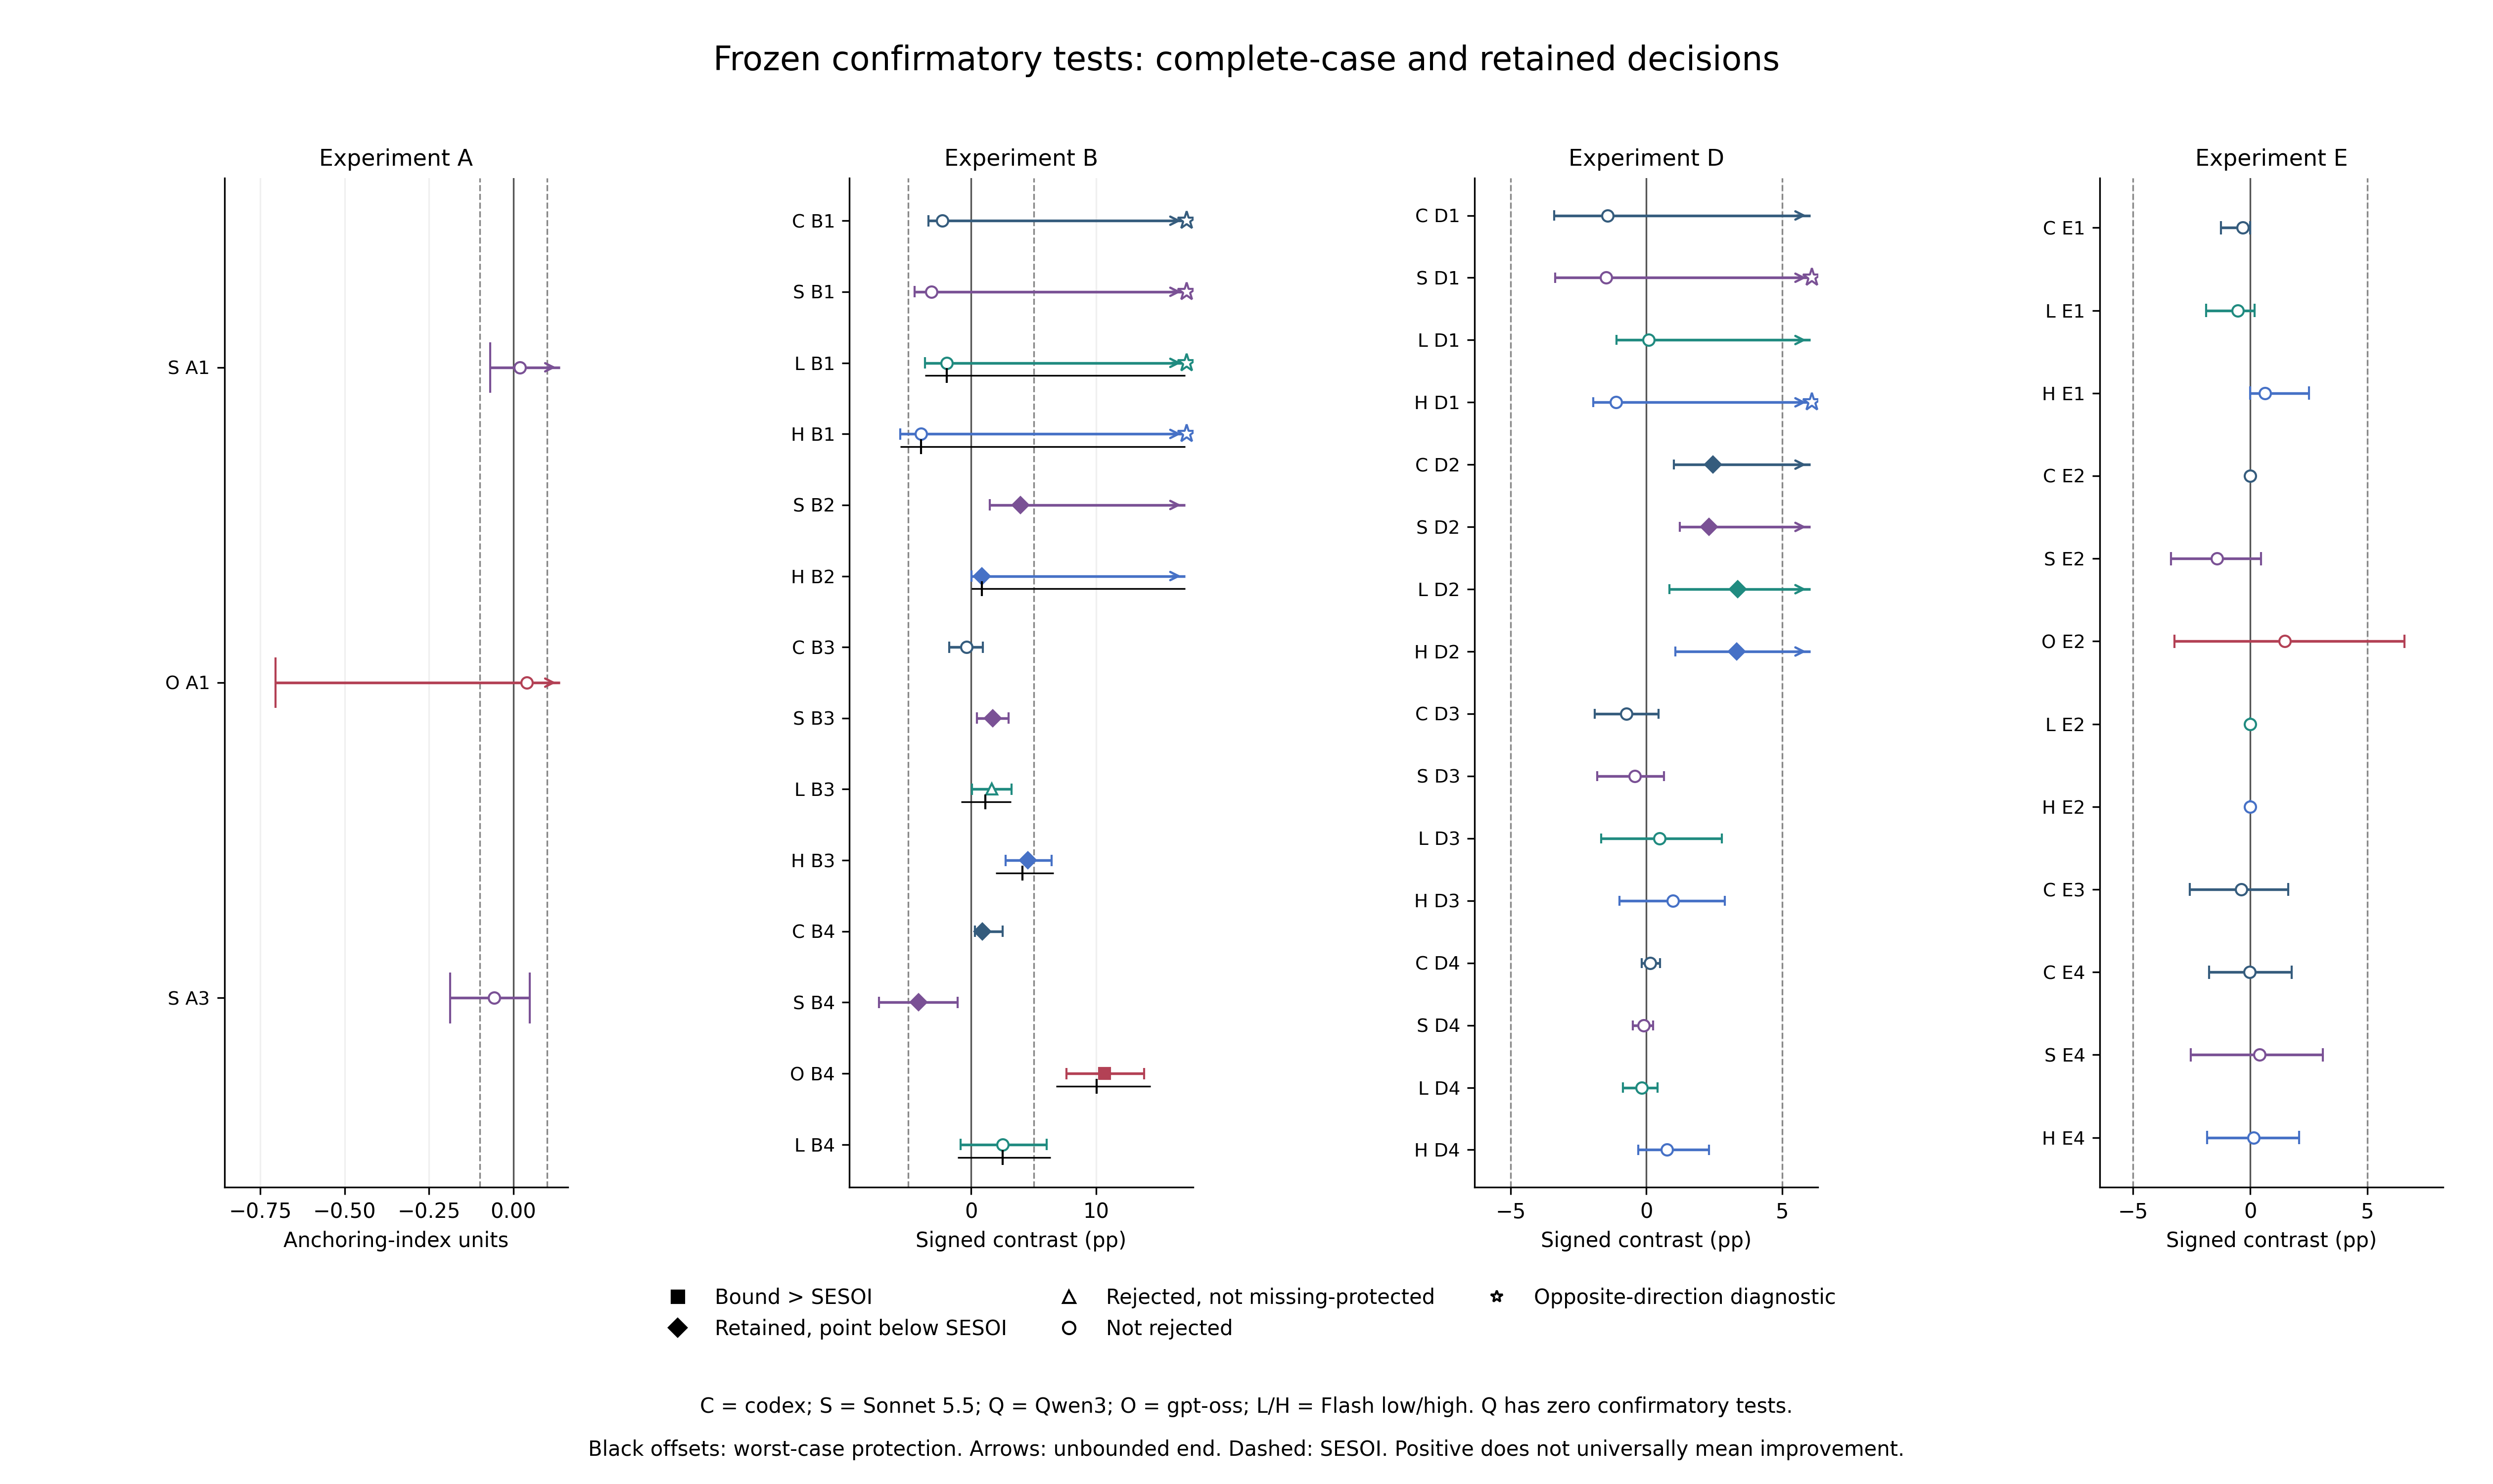
\includegraphics[width=\linewidth,height=.70\textheight,keepaspectratio]{figures/fig1_confirmatory.png}\end{center}
\textbf{Figure 1. All 45 frozen confirmatory tests.} Squares:\allowbreak{} final bound exceeds SESOI; diamonds:\allowbreak{} retained directional point below SESOI; triangles:\allowbreak{} complete-\allowbreak{}case rejection not retained under missingness protection; circles:\allowbreak{} no complete-\allowbreak{}case rejection. Hollow stars mark six opposite-\allowbreak{}direction diagnostic bounds,\allowbreak{} not additional rejections. Colored intervals show complete-\allowbreak{}case Holm-\allowbreak{}step bounds; black offset intervals show protection when required. Arrows indicate unbounded ends. A uses native anchoring-\allowbreak{}index units,\allowbreak{} not factual percentage-\allowbreak{}error reduction; B/\allowbreak{}D/\allowbreak{}E use signed operational contrasts in pp. A positive sign does not universally indicate improvement. Qwen3 forwarded zero hypotheses. Table H2 reports complete numeric results.\par\clearpage

% END M:183

% BEGIN M:185 text

Six reverse-\allowbreak{}bound diagnostics qualify:\allowbreak{} B1 in codex,\allowbreak{} Sonnet,\allowbreak{} Flash low and Flash high,\allowbreak{} and D1 in Sonnet and Flash high. They use rank-\allowbreak{}specific alpha,\allowbreak{} not a fixed 95\% cutoff. They are not six new tests.\par

% END M:185

% BEGIN M:187 text

\subsection{Anchoring and source framing}

% END M:187

% BEGIN M:189 text

The configurations do not exhibit a uniform response to random versus informative-\allowbreak{}source framing. Codex and Sonnet have small mean direct irrelevant-\allowbreak{}anchor indices. Qwen3's paired direct index is approximately 0.946 and falls to 0.338 with multi-\allowbreak{}estimate elicitation; the gpt-\allowbreak{}oss paired index instead rises from 0.039 to 0.197. These are descriptive paired means; single-\allowbreak{}format endpoint denominators can differ.\par

% END M:189

% BEGIN M:191 text

Sonnet A1/\allowbreak{}A3 and gpt-\allowbreak{}oss A1 do not reject. Codex and both Flash A families were downgraded after development known-\allowbreak{}truth screening. Source sensitivity does not measure factual accuracy:\allowbreak{} a model knowing the answer may appropriately ignore an inaccurate informative anchor. Tables H3 and F2 retain the distinction.\par

% END M:191

% BEGIN M:193 text

\subsection{Reconstructed hindsight,\allowbreak{} wording and confirmation error}

% END M:193

% BEGIN M:195 text

Direct b is negative in the four configurations that forwarded B1; reverse adjusted upper bounds are -\allowbreak{}1.23,\allowbreak{} -\allowbreak{}1.84,\allowbreak{} -\allowbreak{}0.29 and -\allowbreak{}2.42 pp in codex,\allowbreak{} Sonnet,\allowbreak{} Flash low and Flash high. This is the operational HI-\allowbreak{}minus-\allowbreak{}F contrast. Public-\allowbreak{}item exposure,\allowbreak{} reconstruction wording and conditioning on noisy prospective ratings remain possible influences; none is identified as the cause of the overall negative means.\par

% END M:195

% BEGIN M:197 text

Removing the ignore instruction while retaining the retrospective question produces retained B2 shifts in Sonnet (+3.93 pp) and Flash high (+0.85 pp). The multi-\allowbreak{}minus-\allowbreak{}direct b shift B3 retains direction in Sonnet and Flash high but not in Flash low after protection. B4 varies by configuration,\allowbreak{} including gpt-\allowbreak{}oss deterioration and Sonnet improvement. Differences in b and e\_\allowbreak{}PO cannot be pooled as a universal attenuation factor. Human ProbCOPA ratings remain descriptive references,\allowbreak{} not normative probability targets.\par

% END M:197

% BEGIN M:199 text

\subsection{Base rates and the direct-\allowbreak{}response ceiling}

% END M:199

% BEGIN M:201 text

All C endpoints are descriptive after the development ceiling. Direct slopes are near one and posterior errors small; displayed 1.000 and 0.000 values are rounded. A slope near one alone is insufficient:\allowbreak{} intercepts and probability error also matter. Multi-\allowbreak{}estimate responses increase paired posterior error in Sonnet by approximately 1.006 pp and in Qwen3 by 0.647 pp,\allowbreak{} while codex error slightly decreases. Elicitation and aggregation change together,\allowbreak{} so increased error does not identify aggregation arithmetic as an isolated mechanism.\par

% END M:201

% BEGIN M:203 text

\subsection{Conjunction presentation and call structure}

% END M:203

% BEGIN M:205 text

Direct separate-\allowbreak{}minus-\allowbreak{}joint signed excess D2 retains confirmation in codex (+2.46 pp),\allowbreak{} Sonnet (+2.30 pp),\allowbreak{} Flash low (+3.37 pp) and Flash high (+3.34 pp),\allowbreak{} all with sub-\allowbreak{}SESOI points. Qwen3 and gpt-\allowbreak{}oss D2 remain descriptive because they were not forwarded. Joint prompts make constraints visible while placing related values in the same call; separate prompts involve independent calls. D2 therefore does not identify constraint visibility alone or confirm a reduction in binary violation rates. D3/\allowbreak{}D4 format contrasts do not yield retained confirmation.\par

% END M:205

% BEGIN M:207 text

\subsection{Status quo,\allowbreak{} defaults and informed advice}

% END M:207

% BEGIN M:209 text

No E test yields retained confirmation. This does not establish absence of a framing effect or equivalence. Several status/\allowbreak{}default means are small under explicit random-\allowbreak{}label provenance and zero switching cost,\allowbreak{} while advice effects remain large. Advice effects decline under multi-\allowbreak{}estimate elicitation in gpt-\allowbreak{}oss and both Flash settings,\allowbreak{} with a different pattern in codex. All formal recommendation controls remain above the 5-\allowbreak{}pp diagnostic threshold; this diagnostic does not remove frozen tests.\par

% END M:209

% BEGIN M:211 text

Formal neutral summaries use 32 distinct items. The development neutral diagnostic uses eight original manifest IDs,\allowbreak{} not E01-\allowbreak{}E08 renumbering; E12 did not cause formal-\allowbreak{}item screening. Tables H3-\allowbreak{}H4 report complete paired subsets,\allowbreak{} controls and supplemental endpoints.\par

% END M:211

% BEGIN M:215 text

\clearpage\begin{center}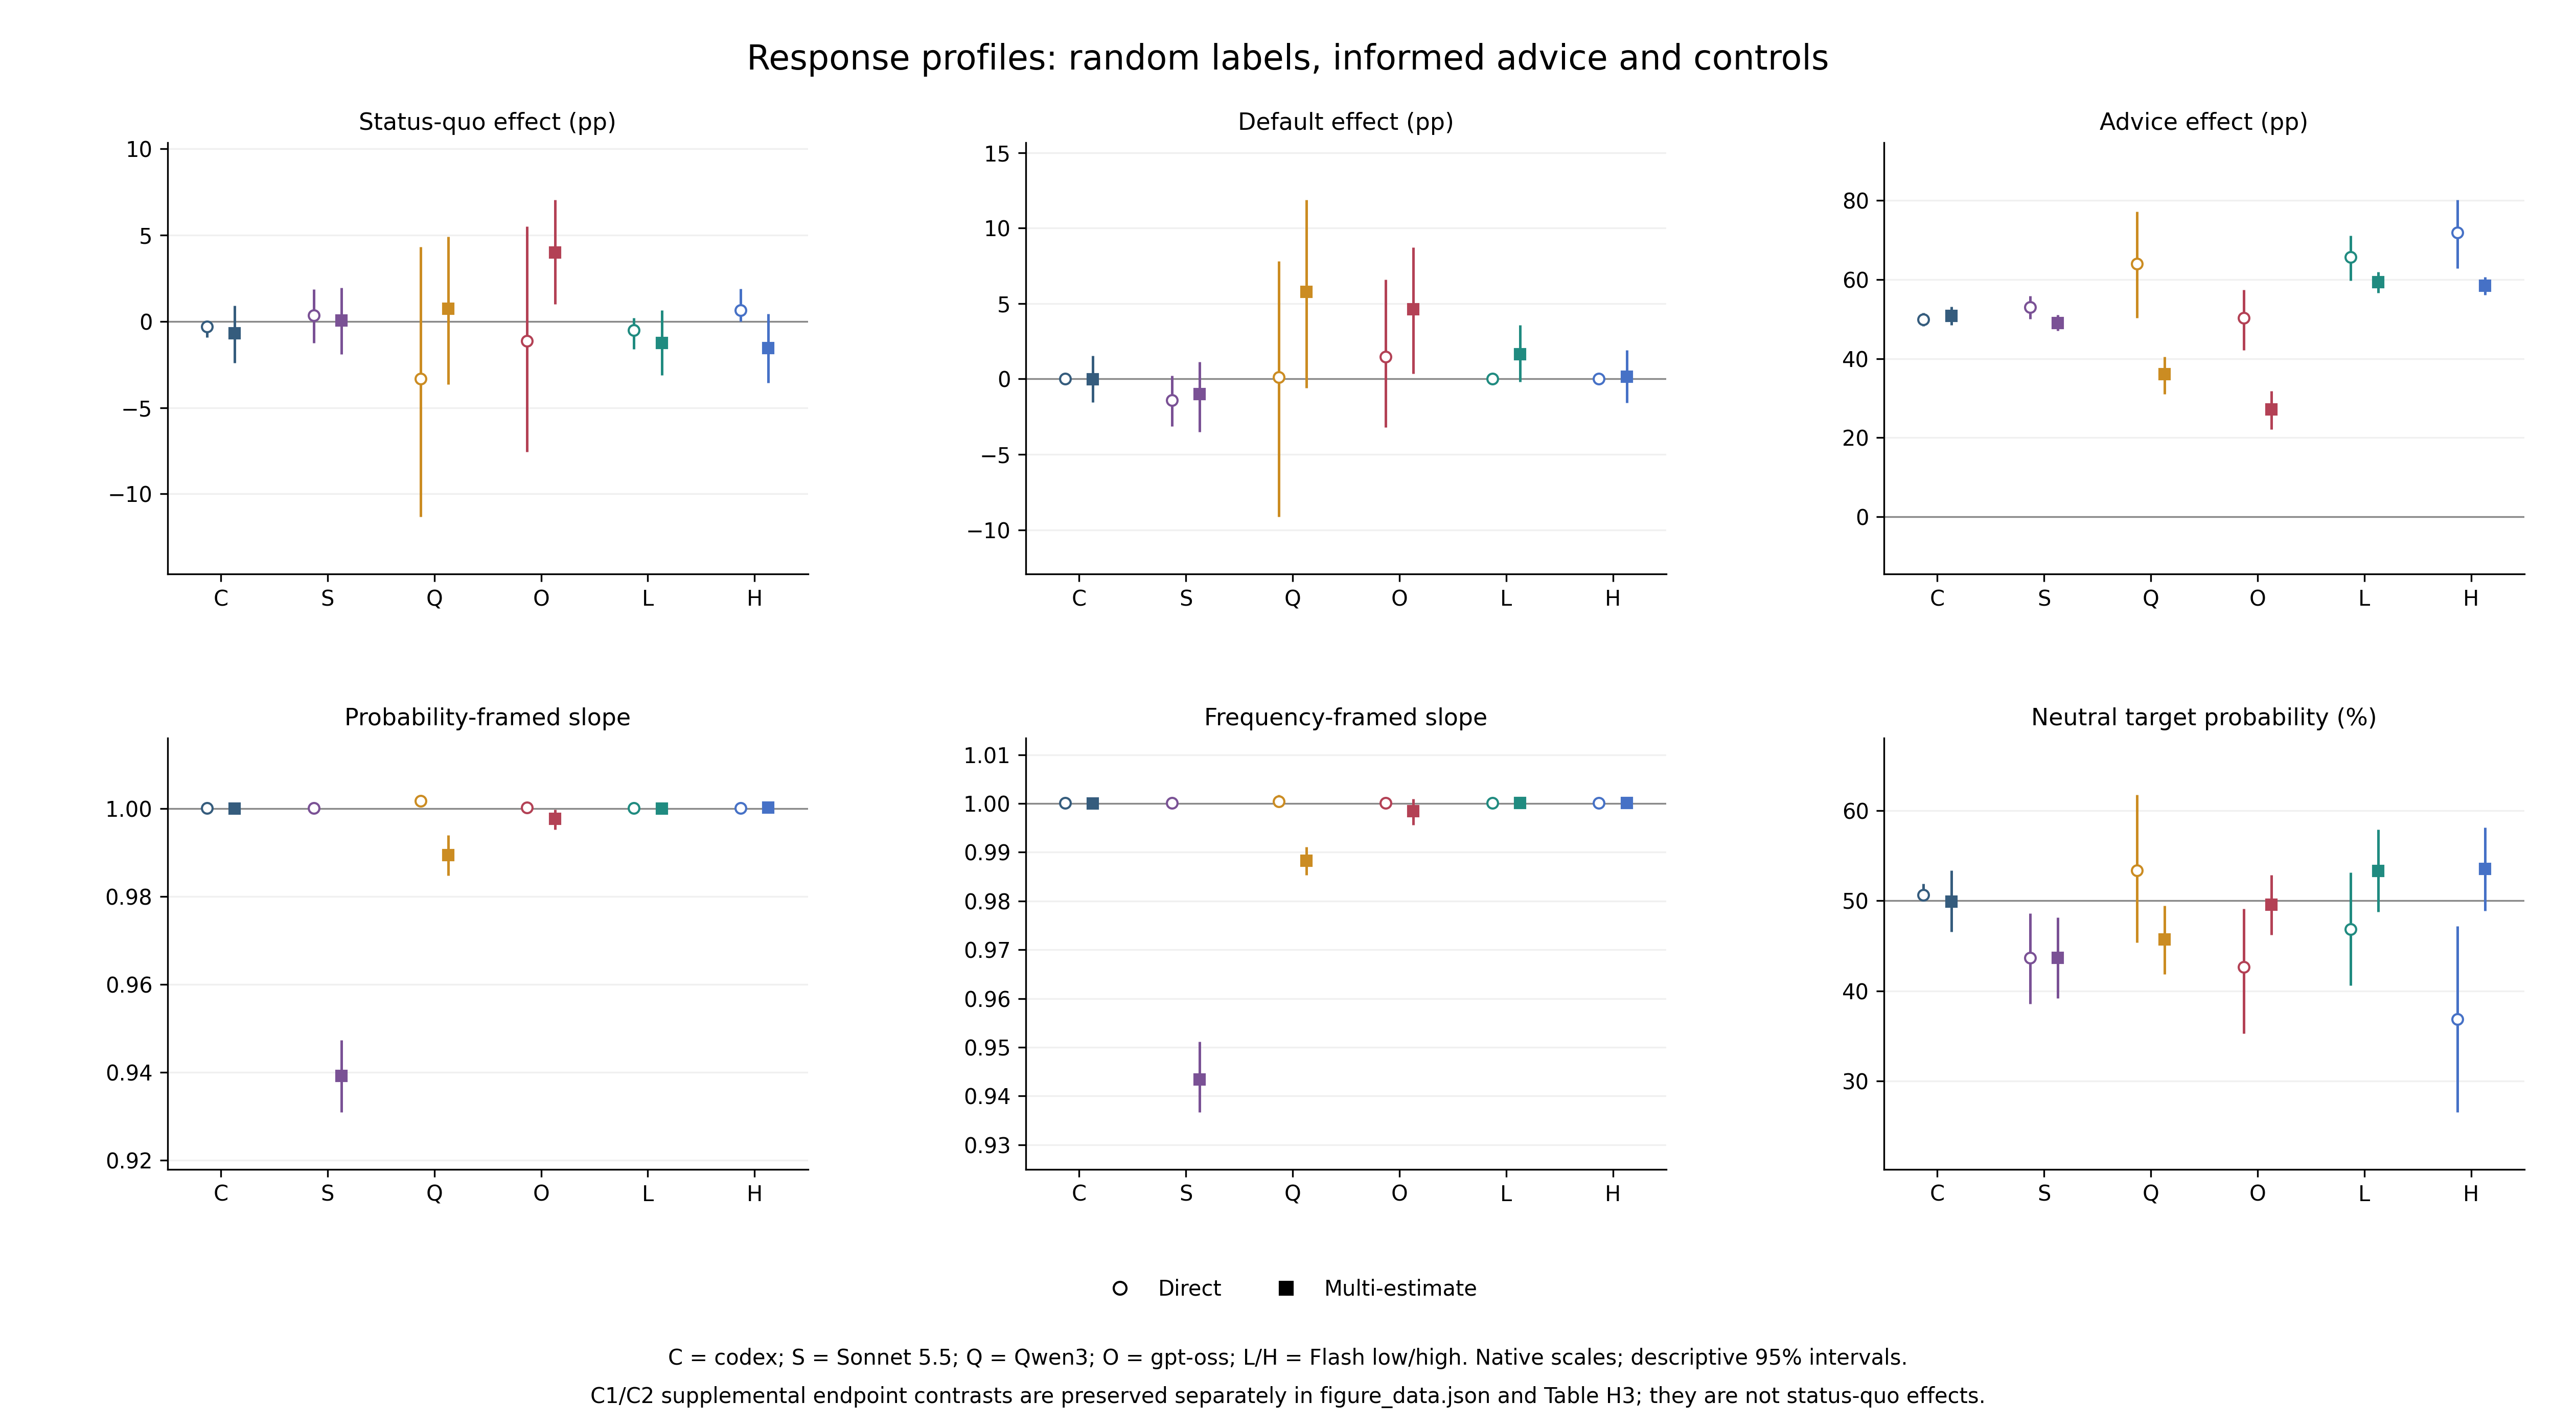
\includegraphics[width=\linewidth,height=.70\textheight,keepaspectratio]{figures/fig2_status_quo_default_advice.png}\end{center}
\textbf{Figure 2. Direct and multi-\allowbreak{}estimate descriptive profiles across six configurations.} Status-\allowbreak{}quo,\allowbreak{} default and advice effects occupy the top panels; C probability/\allowbreak{}frequency slopes and E neutral judgments occupy the lower panels. Intervals are unadjusted 95\% cluster-\allowbreak{}bootstrap intervals. C1 is 1 minus direct probability slope and C2 is direct frequency-\allowbreak{}minus-\allowbreak{}probability slope; they are not status-\allowbreak{}quo endpoints or the underlying slope means. Supplemental C1/\allowbreak{}C2 values are reported separately in H3.\par\clearpage

% END M:215

% BEGIN M:219 text

\clearpage\begin{center}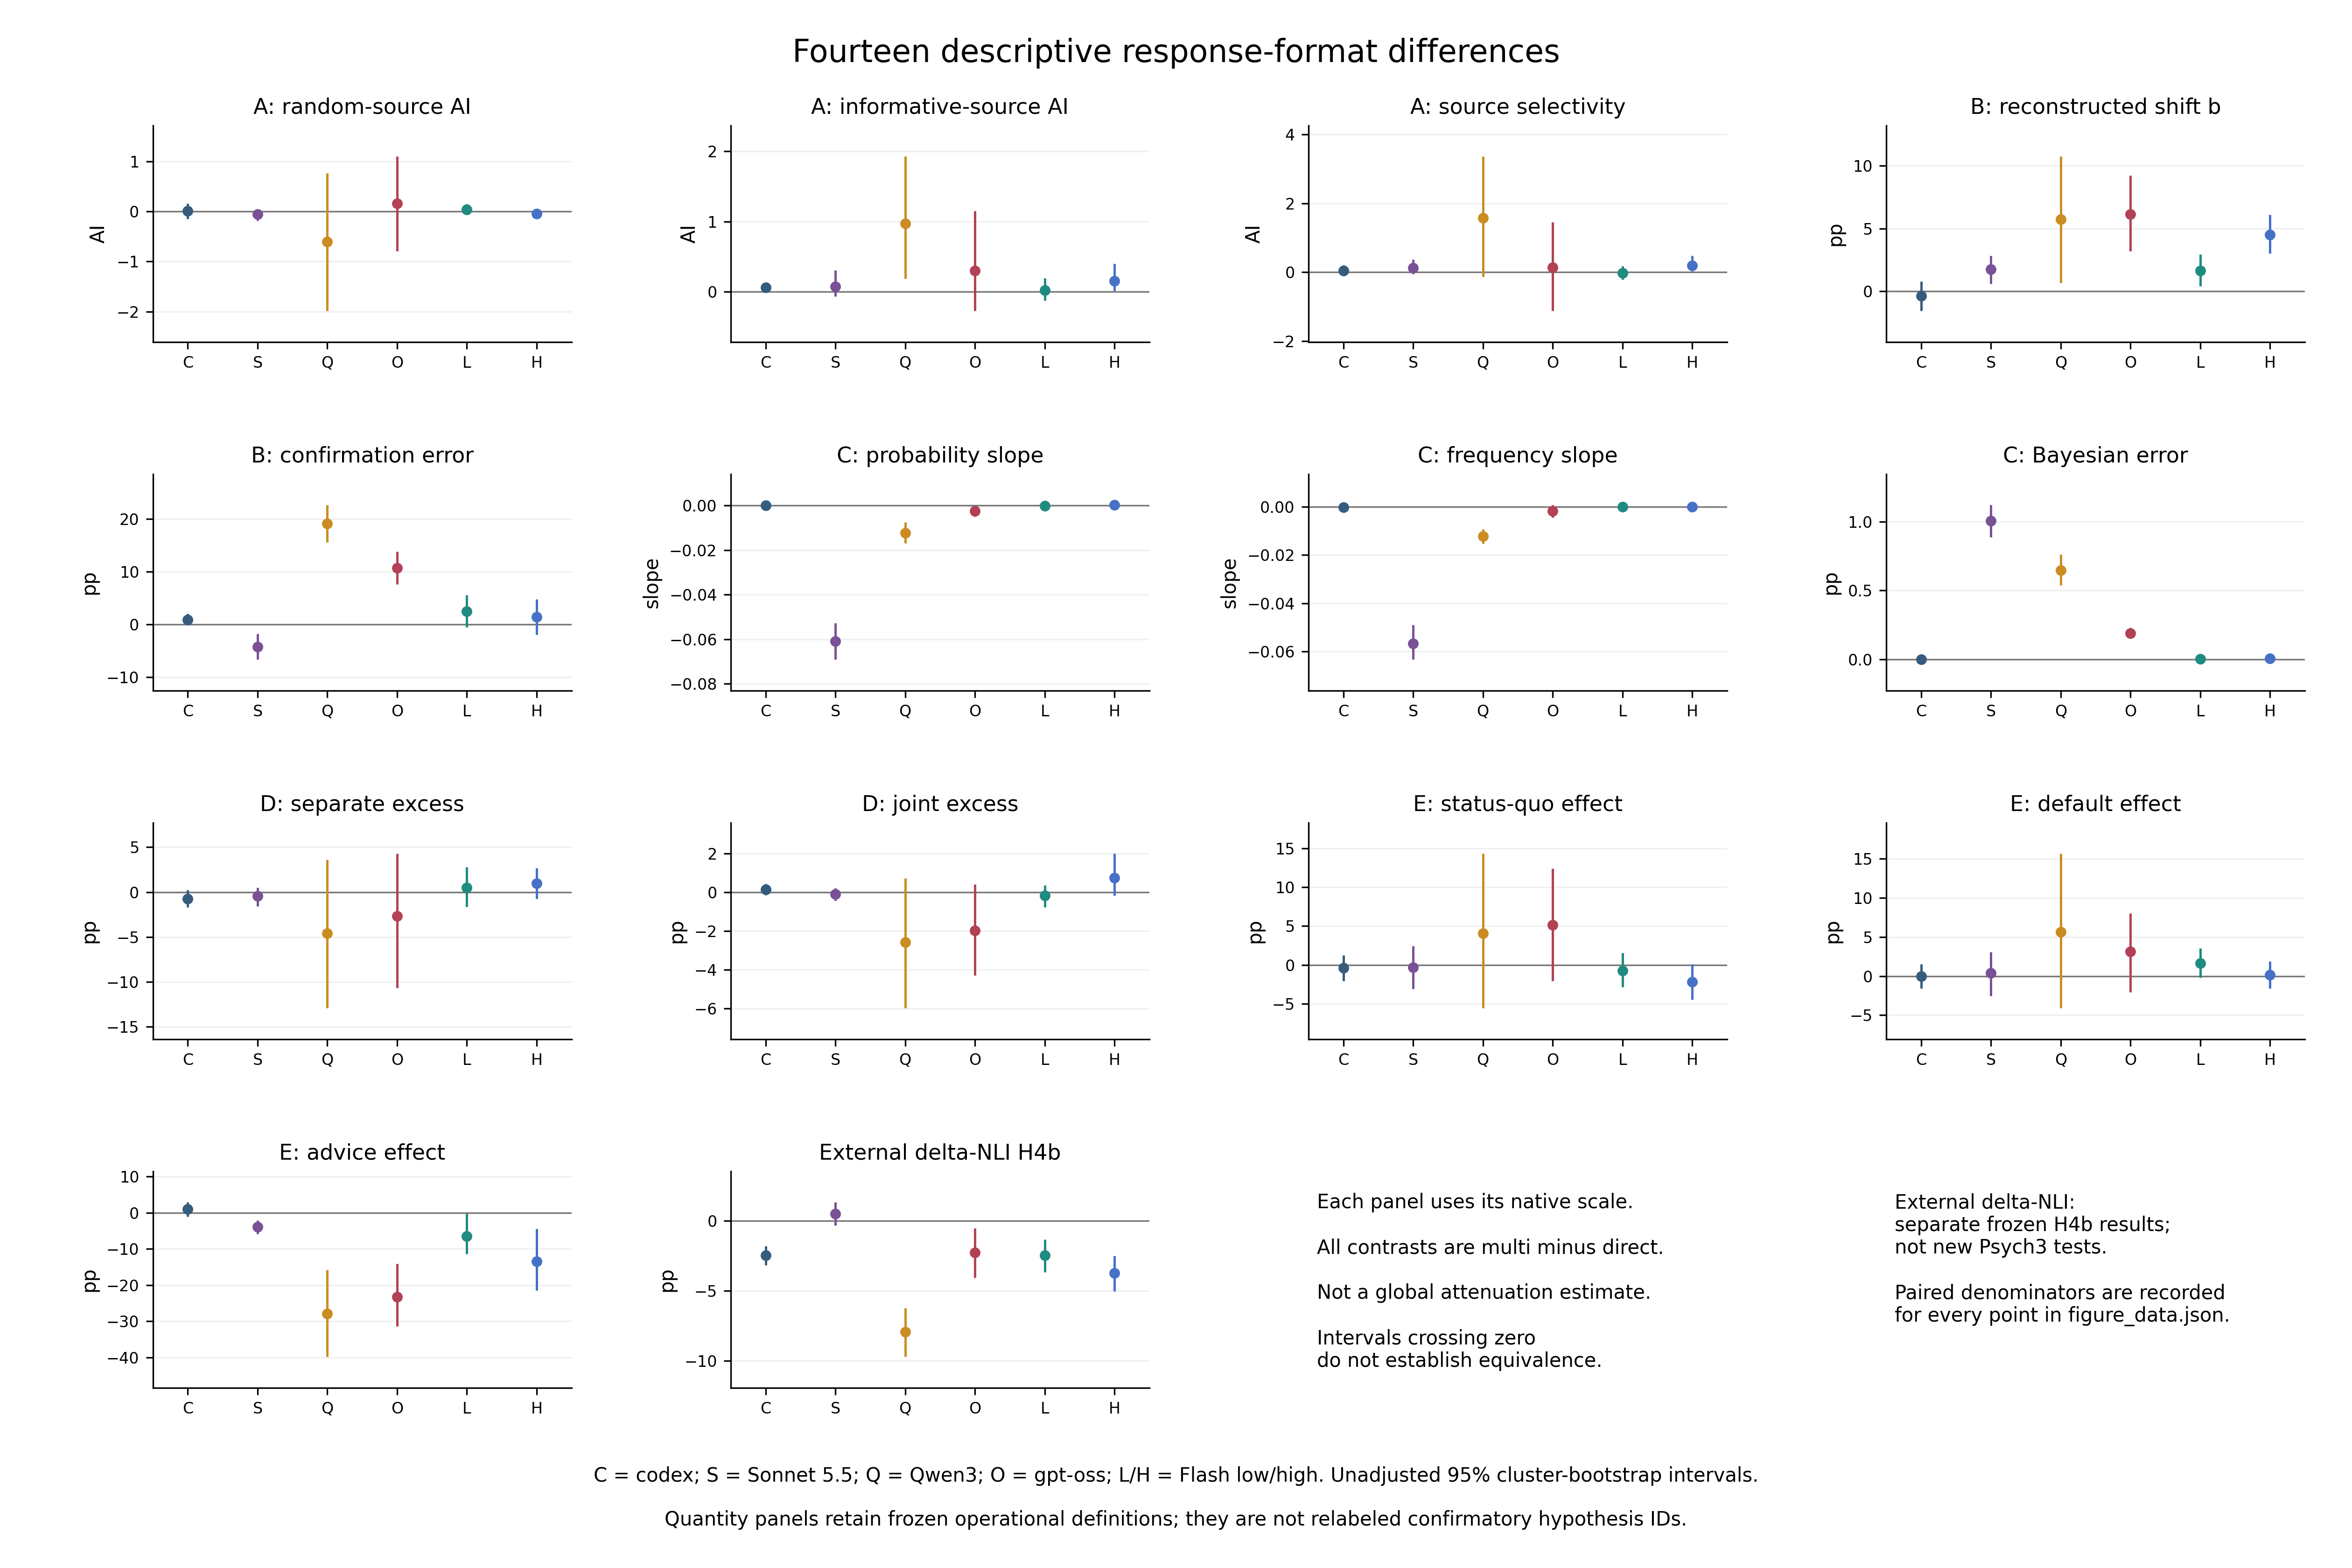
\includegraphics[width=\linewidth,height=.70\textheight,keepaspectratio]{figures/fig3_format_differences.png}\end{center}
\textbf{Figure 3. Fourteen descriptive multi-\allowbreak{}estimate-\allowbreak{}minus-\allowbreak{}direct quantities.} Panels use the physical quantities from the frozen cross-\allowbreak{}experiment export:\allowbreak{} A's irrelevant/\allowbreak{}informative anchoring indices and selectivity; B's b and e\_\allowbreak{}PO; C's probability/\allowbreak{}frequency slopes and Bayesian error; D's separate/\allowbreak{}joint signed excess; E's status/\allowbreak{}default/\allowbreak{}advice effects; and external delta-\allowbreak{}NLI H4b. Each has its own native scale and paired subset. These quantity panels are not identical to confirmatory hypothesis IDs. The external comparison comes from a separate frozen study,\allowbreak{} with a different codex CLI version,\allowbreak{} and is not a new cross-\allowbreak{}task confirmatory test. Intervals crossing zero do not establish equivalence.\par\clearpage

% END M:219

% BEGIN M:221 text

\subsection{Flash-\allowbreak{}high execution windows}

% END M:221

% BEGIN M:223 text

The 3,\allowbreak{}049 F0 and 653 F1 units are disjoint. F0 retains one missing B710 unit; F1 has none. Both inherit one development set of 618 admitted OK units. The combined formal export retains the frozen nine-\allowbreak{}key schema (3,\allowbreak{}718 lines; 3,\allowbreak{}702 admitted; 16 excluded). Material scheduling and execution windows are associated. Cluster D /\allowbreak{} w01 spans F0 (7 r0 calls) and F1 (3 r0 calls) across both response formats. There are zero cross-\allowbreak{}batch r0/\allowbreak{}r1 repeat pairs:\allowbreak{} every repeated unit has its r0 and r1 calls in the same batch. Tables F1 and H11 expose actual frozen condition codes without invented plausible/\allowbreak{}implausible or HI/\allowbreak{}LO renaming.\par

% END M:223

% BEGIN M:225 text

F0 and F1 are non-\allowbreak{}randomized execution windows confounded with item schedule order and collection time. Differences are exploratory and do not identify a causal execution-\allowbreak{}window or model effect.\par

% END M:225

% BEGIN M:227 text

\section{Exploratory and Post-\allowbreak{}Cohort Mechanistic Analyses}

% END M:227

% BEGIN M:229 text

\subsection{Exploratory candidate spread in the six-\allowbreak{}configuration cohort}

% END M:229

% BEGIN M:231 text

Candidate-\allowbreak{}spread analysis was proposed after viewing formal results and is not preregistered. All six configurations use the original pure analyse\_\allowbreak{}items function,\allowbreak{} 5,\allowbreak{}000 cluster-\allowbreak{}bootstrap draws and seed 20261029 on admitted r0 items. The three v1 configurations reproduce their earlier exploratory families with exact JSON value equality. This manuscript-\allowbreak{}generation sandbox reads registered result JSON without opening raw attempt files or the protected original freeze; strict raw admission belongs to the audited host bundle,\allowbreak{} not a new claim by this builder.\par

% END M:231

% BEGIN M:233 text

A spread is weighted candidate log-\allowbreak{}quantity SD,\allowbreak{} while extracted estimates retain the log of the weighted arithmetic mean. B-\allowbreak{}E use probability points. D joint-\allowbreak{}call spread averages the conjunction and B component spreads,\allowbreak{} not four independent calls. Correlations aggregate within item and resample whole clusters. Undefined correlations remain undefined,\allowbreak{} including constant-\allowbreak{}input cases; zero valid resamples are not failed experiments.\par

% END M:233

% BEGIN M:235 text

Tables G1 and H7-\allowbreak{}H10 provide all six distributions,\allowbreak{} pairing denominators,\allowbreak{} spread-\allowbreak{}effect associations,\allowbreak{} A spread-\allowbreak{}error associations and D P/\allowbreak{}W strata. Within-\allowbreak{}sample median splits are descriptions,\allowbreak{} not deployment thresholds. Shared arithmetic inputs,\allowbreak{} difficulty/\allowbreak{}source composition,\allowbreak{} framing and cell availability limit interpretation. Independent task splits,\allowbreak{} targets and difficulty/\allowbreak{}scale baselines are required before claiming predictive utility.\par

% END M:235

% BEGIN M:237 text

\subsection{Post-\allowbreak{}cohort mechanistic follow-\allowbreak{}up:\allowbreak{} Scale granularity and within-\allowbreak{}call elicitation organization}\label{sec:5.2}

% END M:237

% BEGIN M:239 text

\subsubsection{Motivation,\allowbreak{} Stage 2B diagnostic pilot,\allowbreak{} and Stage 2C factorial crossover design}

% END M:239

% BEGIN M:241 text

In the primary six-\allowbreak{}configuration cohort (Section 4),\allowbreak{} Experiment C used structured numerical tables and reached a near-\allowbreak{}ceiling in direct probability mode,\allowbreak{} preventing confirmatory tests of whether multi-\allowbreak{}estimate elicitation mitigates base-\allowbreak{}rate neglect when diagnostic cues are embedded in prose narratives. Moreover,\allowbreak{} across Experiments A--E,\allowbreak{} all probabilities were elicited on the standard $0\text{--}100\%$ scale using an unguided five-\allowbreak{}estimate format (\texttt{ASK\_\allowbreak{}MULTI}) without constraining generation order or permitting repeated candidate values on coarser grids.\par

% END M:241

% BEGIN M:243 text

To examine why unguided \texttt{ASK\_\allowbreak{}MULTI} fails to uniformly debias judgments---and under what representational conditions structured elicitation reduces estimation error---we conducted a two-\allowbreak{}stage post-\allowbreak{}cohort mechanistic investigation via direct REST APIs with thinking disabled (except on the explicit reasoning benchmark \texttt{groq:\allowbreak{}gpt-\allowbreak{}oss-\allowbreak{}120b}). First,\allowbreak{} a four-\allowbreak{}block diagnostic pilot (\textbf{Stage 2B},\allowbreak{} $192 / 192$ valid units per model across \texttt{openai:\allowbreak{}gpt-\allowbreak{}4o-\allowbreak{}mini} and \texttt{sf:\allowbreak{}qwen3-\allowbreak{}8b}) varied within-\allowbreak{}call generation order,\allowbreak{} candidate-\allowbreak{}repeat constraints,\allowbreak{} and scale endpoints ($M \in \{7, 13, 14, 15, 23, 100\}$). Stage 2B identified three specific failure modes of unguided \texttt{ASK\_\allowbreak{}MULTI}:\allowbreak{}
1. \textbf{Unordered Multi-\allowbreak{}Candidate Degradation versus Point-\allowbreak{}First Stabilization (\texttt{Block A})}:\allowbreak{} In narrative Bayesian problems ($n=4$ per cell),\allowbreak{} unguided \texttt{multi\_\allowbreak{}free} increased mean absolute error (MAE) relative to \texttt{direct} on \texttt{openai:\allowbreak{}gpt-\allowbreak{}4o-\allowbreak{}mini} from $10.94\text{ pp}$ to $19.32\text{ pp}$,\allowbreak{} whereas committing to a single point estimate on Line 1 before generating five ordered candidates reduced MAE to $7.34\text{ pp}$ (\texttt{1p5\_\allowbreak{}asc}) and $6.31\text{ pp}$ (\texttt{1p5\_\allowbreak{}desc}),\allowbreak{} and explicit posterior focus reduced MAE to $6.37\text{ pp}$. On \texttt{sf:\allowbreak{}qwen3-\allowbreak{}8b},\allowbreak{} \texttt{1p5\_\allowbreak{}asc} similarly reduced narrative Bayesian MAE from $29.94\text{ pp}$ (\texttt{direct}) and $18.28\text{ pp}$ (\texttt{multi\_\allowbreak{}free}) to $14.76\text{ pp}$.
2. \textbf{Coarse-\allowbreak{}Grid Repulsion and Non-\allowbreak{}Decimal Sweet Spots (\texttt{Blocks B \& D})}:\allowbreak{} On an 8-\allowbreak{}point integer grid ($M=7$,\allowbreak{} integers $\{0, \dots, 7\}$,\allowbreak{} $n=6$ per cell in Block D),\allowbreak{} requiring five distinct candidates (\texttt{multi}) inflated MAE from $6.09\text{ pp}$ (\texttt{direct}) to $14.14\text{ pp}$ on \texttt{openai:\allowbreak{}gpt-\allowbreak{}4o-\allowbreak{}mini} ($3.71\text{ pp}$ to $7.33\text{ pp}$ on the corresponding 8-\allowbreak{}point percentage grid),\allowbreak{} while on \texttt{sf:\allowbreak{}qwen3-\allowbreak{}8b} ($n=4$ in Block B),\allowbreak{} allowing repeated grid values (\texttt{multi\_\allowbreak{}repeat}) reduced $M=7$ MAE from $27.65\text{ pp}$ (\texttt{multi}) to $21.73\text{ pp}$ ($8.61\text{ pp}$ to $6.99\text{ pp}$ on the Block D percentage grid). Meanwhile,\allowbreak{} on scale $M=15$ (Block B,\allowbreak{} $n=4$),\allowbreak{} \texttt{sf:\allowbreak{}qwen3-\allowbreak{}8b} spontaneously used \texttt{.0}/\allowbreak{}\texttt{.5} half-\allowbreak{}integer steps under \texttt{multi},\allowbreak{} lowering MAE from $18.46\text{ pp}$ (\texttt{direct}) to $5.14\text{ pp}$.
3. \textbf{Scale-\allowbreak{}Associated Anchor-\allowbreak{}Shift Reduction (\texttt{Block C})}:\allowbreak{} On two-\allowbreak{}group mixture problems with irrelevant high/\allowbreak{}low anchors ($n=4$ per cell),\allowbreak{} replacing $M=100$ with prime scale $M=13$ reduced the high-\allowbreak{}minus-\allowbreak{}low multi-\allowbreak{}estimate anchoring shift on \texttt{openai:\allowbreak{}gpt-\allowbreak{}4o-\allowbreak{}mini} from $+3.27\text{ pp}$ (\texttt{M100/\allowbreak{}multi}) to $+0.87\text{ pp}$ (\texttt{M13/\allowbreak{}multi}),\allowbreak{} while multi-\allowbreak{}estimate elicitation on $M=13$ lowered anchored MAE relative to \texttt{M13/\allowbreak{}direct} on both \texttt{openai:\allowbreak{}gpt-\allowbreak{}4o-\allowbreak{}mini} ($5.14\text{ pp}$ vs. $11.08\text{ pp}$ under high anchors; $9.70\text{ pp}$ vs. $15.62\text{ pp}$ under low anchors) and \texttt{sf:\allowbreak{}qwen3-\allowbreak{}8b} ($6.36\text{ pp}$ vs. $11.06\text{ pp}$ under high anchors; $5.19\text{ pp}$ vs. $10.87\text{ pp}$ under low anchors).\par

% END M:243

% BEGIN M:248 text

To test whether these observed patterns generalize when scale endpoints and elicitation organization are crossed orthogonally,\allowbreak{} we executed a full \textbf{$5 \times 4 \times 2$ factorial crossover experiment (Stage 2C,\allowbreak{} $280$ units per model; $1,396 / 1,400 = 99.7\%$ valid units across five model families)} crossing:\allowbreak{}
-\allowbreak{} \textbf{Five Bounded Response-\allowbreak{}Scale Ranges ($[0, M]$ with $M \in \{7, 13, 15, 23, 100\}$)}:\allowbreak{} unlike Stage 2B Blocks B and D (which enforced discrete integer grid points),\allowbreak{} Stage 2C prompts specify bounded coordinate ranges $[0, M]$ with decimals permitted (\texttt{Decimals are allowed.}),\allowbreak{} comparing a compact endpoint ($M=7$),\allowbreak{} two prime endpoints ($M=13, 23$),\allowbreak{} a composite non-\allowbreak{}decimal endpoint ($M=15$),\allowbreak{} and the decimal percentage range ($M=100$). All estimates on $[0, M]$ are linearly rescaled to percentage points ($\hat{y}_{\text{pct}} = 100 \cdot \hat{y}_M / M$) for uniform evaluation.
-\allowbreak{} \textbf{Four Elicitation Organizations (\texttt{org})}:\allowbreak{}
  1. \texttt{single}:\allowbreak{} A single direct estimate (\texttt{estimate:\allowbreak{} <0..M>}).
  2. \texttt{multi\_\allowbreak{}repeat}:\allowbreak{} Five weighted candidates on $[0, M]$ summing to weight $1$,\allowbreak{} explicitly permitting repeated candidate values so compact scales are not penalized by distinct-\allowbreak{}point repulsion.
  3. \texttt{1p5\_\allowbreak{}asc\_\allowbreak{}repeat}:\allowbreak{} A point estimate followed by five non-\allowbreak{}decreasing,\allowbreak{} repeat-\allowbreak{}allowed weighted candidates on [0,\allowbreak{}M]; evaluate the five-\allowbreak{}candidate weighted mean. Loose ascending compliance is 329/\allowbreak{}350 (94.0\%); strict five-\allowbreak{}candidate ascending compliance is 324/\allowbreak{}350 (92.6\%),\allowbreak{} including Nemotron 65/\allowbreak{}70. Noncompliant responses remain unsorted and are retained.
  4. \texttt{posterior\_\allowbreak{}focus}:\allowbreak{} An explicit three-\allowbreak{}line belief-\allowbreak{}updating scaffold (\texttt{prior\_\allowbreak{}anchor},\allowbreak{} \texttt{evidence\_\allowbreak{}shift},\allowbreak{} \texttt{final\_\allowbreak{}estimate}) paired with an instruction not to copy raw background percentages as the final estimate; responses that end before emitting an explicit \texttt{final\_\allowbreak{}estimate:\allowbreak{}} line are marked invalid (\texttt{no\_\allowbreak{}final\_\allowbreak{}estimate\_\allowbreak{}label}).
-\allowbreak{} \textbf{Two Objective Ground-\allowbreak{}Truth Task Families ($14$ items per scale $\times$ organization cell)}:\allowbreak{}
  1. \emph{Task 1 --- Narrative Bayesian Updating (\texttt{bayes\_\allowbreak{}narrative},\allowbreak{} $8$ items)}:\allowbreak{} Prose scenarios spanning four prior/\allowbreak{}likelihood-\allowbreak{}ratio regimes (\texttt{low\_\allowbreak{}moderate},\allowbreak{} \texttt{verylow\_\allowbreak{}strong},\allowbreak{} \texttt{high\_\allowbreak{}reverse},\allowbreak{} \texttt{middle\_\allowbreak{}mixed}),\allowbreak{} evaluated by mean absolute error ($\text{MAE} = |\hat{y}_{\text{pct}} - p_{\text{Bayes}}|$) and \textbf{Surface Input-\allowbreak{}Number Echo Rate (\texttt{echo\_\allowbreak{}rate})},\allowbreak{} defined as the proportion of responses whose rescaled percentage (within $\pm 0.75\text{ pp}$) or raw scale value (within $\pm 0.25$ units on $M \ne 100$) reproduces one of the three raw percentages in the narrative (\texttt{prior},\allowbreak{} \texttt{hit\_\allowbreak{}rate},\allowbreak{} or \texttt{false\_\allowbreak{}alarm\_\allowbreak{}rate}).
  2. \emph{Task 3 --- Matched Positive/\allowbreak{}Negative Attribute Framing (\texttt{attribute\_\allowbreak{}framing},\allowbreak{} $3$ pairs $\times 2$ frames $= 6$ items)}:\allowbreak{} Two-\allowbreak{}group weighted mixtures ($60\%$ Group A,\allowbreak{} $40\%$ Group B) with non-\allowbreak{}round normative ground truths $y^* \in \{43\%, 46\%, 57\%\}$ \citep{levin1998all}. In each pair,\allowbreak{} the positive frame (\texttt{pos}) states group success rates $(a\%, b\%)$ and the negative frame (\texttt{neg}) states identical group failure rates $((100-a)\%, (100-b)\%)$,\allowbreak{} while \textbf{both frames ask for the combined probability of the positive outcome}. This design simultaneously measures \textbf{Objective Error ($\text{MAE} = |\hat{y}_{\text{pct}} - y^*|$)} and \textbf{Framing Asymmetry ($\text{FA} = |\hat{y}_{\text{pos}} - \hat{y}_{\text{neg}}|$)} on identical normative targets.\par

% END M:248

% BEGIN M:259 text

\subsubsection{Empirical findings across five model families ($1,396 / 1,400 = 99.7\%$ valid)}

% END M:259

% BEGIN M:261 text

We evaluated five diverse model families spanning three capability regimes:\allowbreak{} (i) an explicit reasoning model (\texttt{groq:\allowbreak{}gpt-\allowbreak{}oss-\allowbreak{}120b},\allowbreak{} configured for OpenAI GPT-\allowbreak{}OSS 120B with low reasoning effort and automatic HTTP-\allowbreak{}429 failover to Cloudflare Workers AI \texttt{@cf/\allowbreak{}openai/\allowbreak{}gpt-\allowbreak{}oss-\allowbreak{}120b} in \texttt{run\_\allowbreak{}stage2c\_\allowbreak{}suite.py}; because per-\allowbreak{}unit backend routing and provider-\allowbreak{}side quantization were not logged in the JSONL output,\allowbreak{} we treat this configuration as a composite API endpoint rather than claiming verified checkpoint equivalence across providers),\allowbreak{} (ii) two frontier non-\allowbreak{}thinking MoE/\allowbreak{}compact models (\texttt{aistudio:\allowbreak{}gemma-\allowbreak{}4-\allowbreak{}26b-\allowbreak{}a4b-\allowbreak{}it},\allowbreak{} Google Gemma 4 26B-\allowbreak{}A4B MoE; and \texttt{openai:\allowbreak{}gpt-\allowbreak{}4o-\allowbreak{}mini}),\allowbreak{} and (iii) two open-\allowbreak{}weight non-\allowbreak{}thinking models spanning 8B to 120B parameters (\texttt{sf:\allowbreak{}qwen3-\allowbreak{}8b},\allowbreak{} Alibaba Qwen 3 8B; and \texttt{nv:\allowbreak{}nemotron-\allowbreak{}3.5-\allowbreak{}super-\allowbreak{}vl-\allowbreak{}120b},\allowbreak{} NVIDIA Nemotron 3.5 120B-\allowbreak{}A12B MoE). All four non-\allowbreak{}thinking models achieved $280 / 280$ ($100.0\%$) valid parses,\allowbreak{} and \texttt{groq:\allowbreak{}gpt-\allowbreak{}oss-\allowbreak{}120b} achieved $276 / 280$ ($98.6\%$) valid parses ($4$ \texttt{posterior\_\allowbreak{}focus} trials on non-\allowbreak{}decimal scales $M \in \{13, 15, 23\}$ ended mid-\allowbreak{}calculation during verbose fraction arithmetic without emitting a \texttt{final\_\allowbreak{}estimate:\allowbreak{}} line; because \texttt{finish\_\allowbreak{}reason} and per-\allowbreak{}request token usage were not logged in the JSONL records,\allowbreak{} these $4$ incomplete responses are marked invalid),\allowbreak{} yielding $1,396 / 1,400$ ($99.7\%$) valid units overall (Table 3,\allowbreak{} Figure 4).\par

% END M:261

% BEGIN M:265 text

\clearpage\begin{center}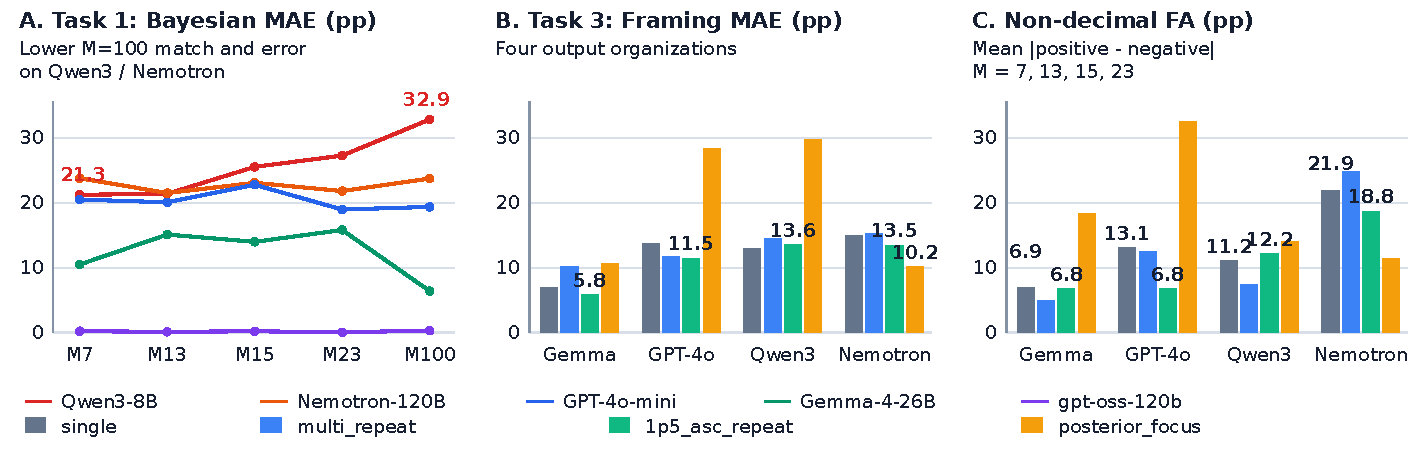
\includegraphics[width=\linewidth,height=.70\textheight,keepaspectratio]{figures/fig4_stage2c_crossover.pdf}\end{center}
\textbf{Figure 4. Stage 2C $5 \times 4 \times 2$ factorial crossover across five model families ($1,396 / 1,400$ valid units).} Panel A shows Narrative Bayesian Updating MAE (\texttt{pp},\allowbreak{} Task 1,\allowbreak{} $n=8$ items/\allowbreak{}cell) and surface percentage-\allowbreak{}token echo rates across response scales $M \in \{7, 13, 15, 23, 100\}$. Panel B shows Attribute Framing objective MAE (\texttt{pp},\allowbreak{} Task 3,\allowbreak{} $n=6$ items/\allowbreak{}cell) across all four elicitation organizations. Panel C shows mean Positive/\allowbreak{}Negative Framing Asymmetry ($\text{FA} = |\hat{y}_{\text{pos}} - \hat{y}_{\text{neg}}|$,\allowbreak{} \texttt{pp}) averaged across the four non-\allowbreak{}decimal scales $M \in \{7, 13, 15, 23\}$.\par\clearpage

% END M:265

% BEGIN M:267 text

\textbf{Table 3. Stage 2C marginal performance across response scales ($M$) and elicitation organizations (\texttt{org}) for all five model families ($1,396 / 1,400$ valid units)}\par

% END M:267

% BEGIN M:269 text

Each scale row pools all valid units across the 4 organizations ($n=32$ units for Task 1 MAE,\allowbreak{} $n=24$ for Task 3 MAE,\allowbreak{} $n=56$ across Task 1 + Task 3 for overall \texttt{echo\_\allowbreak{}rate}; for \texttt{groq:\allowbreak{}gpt-\allowbreak{}oss-\allowbreak{}120b},\allowbreak{} $n=31$ Task 1 on $M \in \{13, 15, 23\}$ and $n=23$ Task 3 on $M=23$). Each organization row pools all valid units across the 5 scales ($n=40$ for Task 1 MAE,\allowbreak{} $n=30$ for Task 3 MAE,\allowbreak{} $n=12$ matched pairs across the 4 non-\allowbreak{}decimal scales for Task 3 Non-\allowbreak{}Decimal $\text{FA}$,\allowbreak{} and $n=70$ across Task 1 + Task 3 for overall \texttt{echo\_\allowbreak{}rate}; for \texttt{groq:\allowbreak{}gpt-\allowbreak{}oss-\allowbreak{}120b} \texttt{posterior\_\allowbreak{}focus},\allowbreak{} $n=37$ Task 1,\allowbreak{} $n=29$ Task 3,\allowbreak{} $n=11$ non-\allowbreak{}decimal $\text{FA}$ pairs,\allowbreak{} and $n=66$ overall). Bold indicates the lowest (best) value within each model $\times$ factor block.\par

% END M:269

% BEGIN M:271 table

\begingroup\scriptsize\setlength{\tabcolsep}{1.3mm}\setlength{\LTpre}{4pt}\setlength{\LTpost}{6pt}
\begin{longtable}{>{\raggedright\arraybackslash}p{14.429mm}>{\raggedright\arraybackslash}p{12.910mm}>{\raggedright\arraybackslash}p{25.820mm}>{\raggedright\arraybackslash}p{25.820mm}>{\raggedright\arraybackslash}p{44.805mm}>{\raggedright\arraybackslash}p{29.617mm}}
\toprule
Model Configuration & Slice /\allowbreak{} Condition & Task 1:\allowbreak{} Bayesian Updating MAE (pp) & Task 3:\allowbreak{} Attribute Framing MAE (pp) & Task 3:\allowbreak{} Non-\allowbreak{}Decimal Mean Framing Asymmetry $\text{FA}$ (pp) & Overall Surface Echo Rate (\texttt{echo\_\allowbreak{}rate}) \\
\midrule\endfirsthead
\toprule
Model Configuration & Slice /\allowbreak{} Condition & Task 1:\allowbreak{} Bayesian Updating MAE (pp) & Task 3:\allowbreak{} Attribute Framing MAE (pp) & Task 3:\allowbreak{} Non-\allowbreak{}Decimal Mean Framing Asymmetry $\text{FA}$ (pp) & Overall Surface Echo Rate (\texttt{echo\_\allowbreak{}rate}) \\
\midrule\endhead
\bottomrule\endfoot
\textbf{\texttt{groq:\allowbreak{}gpt-\allowbreak{}oss-\allowbreak{}120b}} & Scale $M=7$ & 0.23 & 0.15 & --- & \textbf{0.0\%} \\
\emph{(Reasoning model; 276 /\allowbreak{} 280)} & Scale $M=13$ (prime) & 0.13 & 0.19 & --- & 1.8\% \\
 & Scale $M=15$ & 0.22 & 0.04 & --- & \textbf{0.0\%} \\
 & Scale $M=23$ (prime) & \textbf{0.06} & 0.05 & --- & \textbf{0.0\%} \\
 & Scale $M=100$ (decimal) & 0.32 & \textbf{0.02} & --- & \textbf{0.0\%} \\
 & Org:\allowbreak{} \texttt{single} & 0.07 & \textbf{0.01} & \textbf{0.00} & \textbf{0.0\%} \\
 & Org:\allowbreak{} \texttt{multi\_\allowbreak{}repeat} & 0.16 & 0.12 & 0.21 & \textbf{0.0\%} \\
 & Org:\allowbreak{} \texttt{1p5\_\allowbreak{}asc\_\allowbreak{}repeat} & 0.49 & 0.13 & 0.17 & \textbf{0.0\%} \\
 & Org:\allowbreak{} \texttt{posterior\_\allowbreak{}focus} \emph{(66/\allowbreak{}70)} & \textbf{0.03} & 0.11 & 0.23 & 1.5\% \\
\textbf{\texttt{aistudio:\allowbreak{}gemma-\allowbreak{}4-\allowbreak{}26b-\allowbreak{}a4b-\allowbreak{}it}} & Scale $M=7$ & 10.51 & 13.04 & --- & 17.9\% \\
\emph{(Frontier MoE; 280 /\allowbreak{} 280)} & Scale $M=13$ (prime) & 15.13 & 8.58 & --- & 10.7\% \\
 & Scale $M=15$ & 14.01 & 8.39 & --- & 7.1\% \\
 & Scale $M=23$ (prime) & 15.84 & 6.78 & --- & 7.1\% \\
 & Scale $M=100$ (decimal) & \textbf{6.42} & \textbf{5.25} & --- & \textbf{1.8\%} \\
 & Org:\allowbreak{} \texttt{single} & 11.09 & 6.98 & 6.94 & 7.1\% \\
 & Org:\allowbreak{} \texttt{multi\_\allowbreak{}repeat} & 13.17 & 10.22 & \textbf{4.99} & 10.0\% \\
 & Org:\allowbreak{} \textbf{\texttt{1p5\_\allowbreak{}asc\_\allowbreak{}repeat}} & \textbf{9.88} & \textbf{5.84} & 6.78 & \textbf{1.4\%} \\
 & Org:\allowbreak{} \texttt{posterior\_\allowbreak{}focus} & 15.39 & 10.60 & 18.41 & 17.1\% \\
\textbf{\texttt{openai:\allowbreak{}gpt-\allowbreak{}4o-\allowbreak{}mini}} & Scale $M=7$ & 20.53 & 20.28 & --- & \textbf{3.6\%} \\
\emph{(Compact commercial; 280 /\allowbreak{} 280)} & Scale $M=13$ (prime) & 20.11 & 15.13 & --- & 7.1\% \\
 & Scale $M=15$ & 22.81 & 18.84 & --- & 14.3\% \\
 & Scale $M=23$ (prime) & \textbf{18.99} & 19.28 & --- & \textbf{3.6\%} \\
 & Scale $M=100$ (decimal) & 19.40 & \textbf{8.18} & --- & 14.3\% \\
 & Org:\allowbreak{} \texttt{single} & \textbf{15.70} & 13.71 & 13.07 & 11.4\% \\
 & Org:\allowbreak{} \texttt{multi\_\allowbreak{}repeat} & 21.07 & 11.69 & 12.58 & \textbf{5.7\%} \\
 & Org:\allowbreak{} \textbf{\texttt{1p5\_\allowbreak{}asc\_\allowbreak{}repeat}} & 19.33 & \textbf{11.49} & \textbf{6.79} & 7.1\% \\
 & Org:\allowbreak{} \texttt{posterior\_\allowbreak{}focus} & 25.36 & 28.48 & 32.55 & 10.0\% \\
\textbf{\texttt{nv:\allowbreak{}nemotron-\allowbreak{}3.5-\allowbreak{}super-\allowbreak{}vl-\allowbreak{}120b}} & Scale $M=7$ & 23.82 & 20.15 & --- & 14.3\% \\
\emph{(120B-\allowbreak{}A12B MoE non-\allowbreak{}think; 280 /\allowbreak{} 280)} & Scale $M=13$ (prime) & \textbf{21.54} & 11.29 & --- & 10.7\% \\
 & Scale $M=15$ & 23.11 & 14.47 & --- & \textbf{8.9\%} \\
 & Scale $M=23$ (prime) & 21.84 & 13.82 & --- & 10.7\% \\
 & Scale $M=100$ (decimal) & 23.77 & \textbf{7.63} & --- & 10.7\% \\
 & Org:\allowbreak{} \texttt{single} & 24.05 & 14.92 & 21.93 & 8.6\% \\
 & Org:\allowbreak{} \texttt{multi\_\allowbreak{}repeat} & 24.80 & 15.31 & 24.93 & 15.7\% \\
 & Org:\allowbreak{} \texttt{1p5\_\allowbreak{}asc\_\allowbreak{}repeat} & 25.68 & 13.51 & 18.75 & 12.9\% \\
 & Org:\allowbreak{} \textbf{\texttt{posterior\_\allowbreak{}focus}} & \textbf{16.73} & \textbf{10.15} & \textbf{11.42} & \textbf{7.1\%} \\
\textbf{\texttt{sf:\allowbreak{}qwen3-\allowbreak{}8b}} & Scale $M=7$ & \textbf{21.27} & 21.24 & --- & 8.9\% \\
\emph{(8B Dense non-\allowbreak{}think; 280 /\allowbreak{} 280)} & Scale $M=13$ (prime) & 21.41 & 14.36 & --- & 7.1\% \\
 & Scale $M=15$ & 25.57 & 20.35 & --- & 14.3\% \\
 & Scale $M=23$ (prime) & 27.31 & 22.06 & --- & \textbf{3.6\%} \\
 & Scale $M=100$ (decimal) & 32.88 & \textbf{10.72} & --- & 32.1\% \\
 & Org:\allowbreak{} \texttt{single} & 26.25 & \textbf{12.98} & 11.15 & 18.6\% \\
 & Org:\allowbreak{} \texttt{multi\_\allowbreak{}repeat} & \textbf{23.34} & 14.59 & \textbf{7.36} & 11.4\% \\
 & Org:\allowbreak{} \texttt{1p5\_\allowbreak{}asc\_\allowbreak{}repeat} & 25.66 & 13.59 & 12.22 & \textbf{10.0\%} \\
 & Org:\allowbreak{} \texttt{posterior\_\allowbreak{}focus} & 27.49 & 29.83 & 14.02 & 12.9\% \\
\end{longtable}
\endgroup

% END M:271

% BEGIN M:319 text

\textbf{1. Observable surface percentage-\allowbreak{}token matches and error.} On Qwen3-\allowbreak{}8B,\allowbreak{} M=100 is associated with high surface percentage-\allowbreak{}token match rates:\allowbreak{} 43.8\% (14/\allowbreak{}32) in narrative Bayesian trials and 32.1\% (18/\allowbreak{}56) overall,\allowbreak{} with Bayesian MAE 32.88 pp (37.3 pp under \texttt{single}). Non-\allowbreak{}decimal endpoints lower surface percentage-\allowbreak{}token match rates:\allowbreak{} Bayesian rates are 6.2\% at M=7,\allowbreak{} 9.4\% at M=13 and 0.0\% at M=23; overall rates range 3.6\%--8.9\%. Bayesian MAE is 21.27,\allowbreak{} 21.41 and 27.31 pp,\allowbreak{} improvements of 11.61,\allowbreak{} 11.47 and 5.57 pp relative to M=100. Cell-\allowbreak{}level errors reach 17.6 pp at M=7 \texttt{single} and 16.7 pp at M=13 \texttt{posterior\_\allowbreak{}focus}. Nemotron achieves 21.54 /\allowbreak{} 21.84 pp at M=13 /\allowbreak{} 23 versus 23.77 pp at M=100; GPT-\allowbreak{}4o-\allowbreak{}mini achieves 18.99 pp at M=23 versus 19.40 pp at M=100. Attribute-\allowbreak{}framing MAE,\allowbreak{} however,\allowbreak{} is lowest at M=100 for every model. A match-\allowbreak{}rate change cannot alone distinguish reduced psychological copying (a hypothesis) from changed scale-\allowbreak{}grid accessibility. P1 independently tests this distinction below.\par

% END M:319

% BEGIN M:321 text

\textbf{2. \texttt{1p5\_\allowbreak{}asc\_\allowbreak{}repeat} as a Structural Stabilizer Relative to Unguided \texttt{multi\_\allowbreak{}repeat}.}  
Across the four non-\allowbreak{}ceiling models,\allowbreak{} unguided \texttt{multi\_\allowbreak{}repeat} exhibits a trade-\allowbreak{}off between smoothing framing noise in Task 3 and suffering from candidate dispersion in Task 1. By contrast,\allowbreak{} \textbf{\texttt{1p5\_\allowbreak{}asc\_\allowbreak{}repeat}}---which commits the model to a single point estimate on Line 1 before eliciting five non-\allowbreak{}decreasing repeat-\allowbreak{}allowed candidates---outperforms \texttt{multi\_\allowbreak{}repeat} on Attribute Framing MAE across all four non-\allowbreak{}ceiling models ($5.84$ vs. $10.22\text{ pp}$ on \texttt{gemma-\allowbreak{}4-\allowbreak{}26b-\allowbreak{}a4b-\allowbreak{}it},\allowbreak{} $11.49$ vs. $11.69\text{ pp}$ on \texttt{gpt-\allowbreak{}4o-\allowbreak{}mini},\allowbreak{} $13.51$ vs. $15.31\text{ pp}$ on \texttt{nemotron-\allowbreak{}120b},\allowbreak{} and $13.59$ vs. $14.59\text{ pp}$ on \texttt{qwen3-\allowbreak{}8b}),\allowbreak{} while on Task 1 (\texttt{bayes\_\allowbreak{}narrative}) it improves over \texttt{multi\_\allowbreak{}repeat} on \texttt{gemma-\allowbreak{}4-\allowbreak{}26b-\allowbreak{}a4b-\allowbreak{}it} ($9.88$ vs. $13.17\text{ pp}$) and \texttt{gpt-\allowbreak{}4o-\allowbreak{}mini} ($19.33$ vs. $21.07\text{ pp}$,\allowbreak{} where \texttt{single} remains lowest at $15.70\text{ pp}$),\allowbreak{} whereas \texttt{multi\_\allowbreak{}repeat} stays slightly lower on \texttt{qwen3-\allowbreak{}8b} ($23.34$ vs. $25.66\text{ pp}$) and \texttt{nemotron-\allowbreak{}120b} ($24.80$ vs. $25.68\text{ pp}$):\allowbreak{}
-\allowbreak{} On \textbf{\texttt{aistudio:\allowbreak{}gemma-\allowbreak{}4-\allowbreak{}26b-\allowbreak{}a4b-\allowbreak{}it}},\allowbreak{} \texttt{1p5\_\allowbreak{}asc\_\allowbreak{}repeat} achieves the lowest marginal Bayesian Updating MAE (\textbf{$9.88\text{ pp}$} vs. $11.09\text{ pp}$ \texttt{single} and $13.17\text{ pp}$ \texttt{multi\_\allowbreak{}repeat}),\allowbreak{} lowest Attribute Framing MAE (\textbf{$5.84\text{ pp}$} vs. $6.98\text{ pp}$ \texttt{single} and $10.22\text{ pp}$ \texttt{multi\_\allowbreak{}repeat}),\allowbreak{} and lowest surface echo rate (\textbf{$1.4\%$}). At compact scale $M=7$,\allowbreak{} \texttt{1p5\_\allowbreak{}asc\_\allowbreak{}repeat} reduces Gemma-\allowbreak{}4's Bayesian MAE to \textbf{$6.5\text{ pp}$} (compared with $10.5\text{ pp}$ under \texttt{single} and $15.95\text{ pp}$ under \texttt{multi\_\allowbreak{}repeat}); on non-\allowbreak{}decimal scales $M=13, 15, 23$,\allowbreak{} it reduces Attribute Framing MAE to \textbf{$5.0\text{ pp}$},\allowbreak{} \textbf{$3.7\text{ pp}$},\allowbreak{} and \textbf{$3.8\text{ pp}$},\allowbreak{} matching the decimal $M=100$ baseline ($3.6\text{ pp}$).
-\allowbreak{} On \textbf{\texttt{openai:\allowbreak{}gpt-\allowbreak{}4o-\allowbreak{}mini}},\allowbreak{} \texttt{1p5\_\allowbreak{}asc\_\allowbreak{}repeat} achieves the lowest marginal Attribute Framing MAE (\textbf{$11.49\text{ pp}$} vs. $13.71\text{ pp}$ \texttt{single}) and \textbf{cuts Positive/\allowbreak{}Negative Framing Asymmetry ($\text{FA}$) nearly in half across the four non-\allowbreak{}decimal scales $M \in \{7, 13, 15, 23\}$},\allowbreak{} reducing mean non-\allowbreak{}decimal $\text{FA}$ from \textbf{$13.07\text{ pp}$} (\texttt{single}) and \textbf{$12.58\text{ pp}$} (\texttt{multi\_\allowbreak{}repeat}) to \textbf{$6.79\text{ pp}$} (at $M=7$,\allowbreak{} $\text{FA}$ drops from $20.95\text{ pp}$ to \textbf{$5.1\text{ pp}$},\allowbreak{} while objective MAE drops from $21.3\text{ pp}$ to \textbf{$13.2\text{ pp}$}).
-\allowbreak{} On \textbf{\texttt{nv:\allowbreak{}nemotron-\allowbreak{}3.5-\allowbreak{}super-\allowbreak{}vl-\allowbreak{}120b}},\allowbreak{} \texttt{1p5\_\allowbreak{}asc\_\allowbreak{}repeat} reduces Attribute Framing MAE from $14.92\text{ pp}$ (\texttt{single}) and $15.31\text{ pp}$ (\texttt{multi\_\allowbreak{}repeat}) to \textbf{$13.51\text{ pp}$} and reduces non-\allowbreak{}decimal Framing Asymmetry from $21.93\text{ pp}$ (\texttt{single}) and $24.93\text{ pp}$ (\texttt{multi\_\allowbreak{}repeat}) to \textbf{$18.75\text{ pp}$} (with prime scales $M=13$ and $M=23$ improving from $12.8\text{ pp}$ and $16.5\text{ pp}$ MAE under \texttt{single} to \textbf{$9.9\text{ pp}$} and \textbf{$10.7\text{ pp}$} under \texttt{1p5\_\allowbreak{}asc\_\allowbreak{}repeat}).\par

% END M:321

% BEGIN M:327 text

\textbf{3. Three-\allowbreak{}Tier Capability Spectrum and the Role of \texttt{posterior\_\allowbreak{}focus}.}  
Comparing \texttt{posterior\_\allowbreak{}focus} across all five models reveals how explicit decomposition interacts with model scale and configuration:\allowbreak{}
-\allowbreak{} \emph{Tier 1 (Reasoning Ceiling and Incomplete Decomposition Responses --- \texttt{groq:\allowbreak{}gpt-\allowbreak{}oss-\allowbreak{}120b})}:\allowbreak{} On this explicit reasoning configuration,\allowbreak{} completed outputs achieve near-\allowbreak{}zero error across \textbf{all five scales and all four organizations} on completed responses (marginal $\text{MAE} \le 0.49\text{ pp}$,\allowbreak{} cell-\allowbreak{}level $\text{MAE} \le 0.97\text{ pp}$,\allowbreak{} and non-\allowbreak{}decimal $\text{FA} \le 0.23\text{ pp}$,\allowbreak{} with \texttt{posterior\_\allowbreak{}focus} achieving $0.03\text{ pp}$ Bayesian MAE and $0.11\text{ pp}$ Attribute Framing MAE across its $66 / 70$ valid responses). On $4 / 70$ \texttt{posterior\_\allowbreak{}focus} trials on non-\allowbreak{}decimal scales ($M \in \{13, 15, 23\}$),\allowbreak{} the response ended mid-\allowbreak{}calculation during verbose fraction arithmetic without emitting a \texttt{final\_\allowbreak{}estimate:\allowbreak{}} line (consistent with output truncation,\allowbreak{} though \texttt{finish\_\allowbreak{}reason} and per-\allowbreak{}request token usage were not logged in the JSONL records).
-\allowbreak{} \emph{Tier 2 (Large MoE with Decomposition-\allowbreak{}Associated Gains --- \texttt{nv:\allowbreak{}nemotron-\allowbreak{}3.5-\allowbreak{}super-\allowbreak{}vl-\allowbreak{}120b})}:\allowbreak{} When a high-\allowbreak{}capacity 120B MoE model operates with thinking disabled,\allowbreak{} it achieves substantially lower error once prompted to decompose the update,\allowbreak{} and \textbf{\texttt{posterior\_\allowbreak{}focus} achieves the best marginal performance across every metric}:\allowbreak{} cutting Bayesian MAE from $24.05\text{ pp}$ (\texttt{single}) to \textbf{$16.73\text{ pp}$} ($12.7\text{ pp}$ at $M=7$,\allowbreak{} $14.9\text{ pp}$ at $M=13$,\allowbreak{} $15.5\text{ pp}$ at $M=23$),\allowbreak{} cutting Attribute Framing MAE from $14.92\text{ pp}$ to \textbf{$10.15\text{ pp}$},\allowbreak{} and cutting non-\allowbreak{}decimal Framing Asymmetry from $21.93\text{ pp}$ to \textbf{$11.42\text{ pp}$}.
-\allowbreak{} \emph{Tier 3 (Compact Non-\allowbreak{}Thinking Models --- \texttt{openai:\allowbreak{}gpt-\allowbreak{}4o-\allowbreak{}mini} and \texttt{sf:\allowbreak{}qwen3-\allowbreak{}8b})}:\allowbreak{} On smaller non-\allowbreak{}thinking models,\allowbreak{} \texttt{posterior\_\allowbreak{}focus} improves \textbf{non-\allowbreak{}linear Bayesian updating on prime scale $M=13$} ($23.6 \to 16.6\text{ pp}$ on \texttt{gpt-\allowbreak{}4o-\allowbreak{}mini}; $23.0 \to 16.7\text{ pp}$ on \texttt{qwen3-\allowbreak{}8b}),\allowbreak{} but induces \textbf{over-\allowbreak{}shifting on linear weighted mixtures} (Task 3),\allowbreak{} where \texttt{1p5\_\allowbreak{}asc\_\allowbreak{}repeat} provides more stable domain-\allowbreak{}general performance.\par

% END M:327

% BEGIN M:334 text

\textbf{Format validity and model heterogeneity.} Nemotron single-\allowbreak{}line collapse falls from 55/\allowbreak{}70 (78.6\%) under unordered \texttt{multi\_\allowbreak{}repeat} to 5/\allowbreak{}70 (7.1\%) under \texttt{1p5\_\allowbreak{}asc\_\allowbreak{}repeat}; this comparison concerns two multi-\allowbreak{}candidate protocols. Across five models,\allowbreak{} fewer-\allowbreak{}than-\allowbreak{}five candidate responses fall from 58/\allowbreak{}350 (16.6\%) to 6/\allowbreak{}350 (1.7\%). Pooled attribute-\allowbreak{}framing MAE is 8.91 pp for Upgraded MCW-\allowbreak{}Asc,\allowbreak{} versus Direct 9.72,\allowbreak{} Direct-\allowbreak{}CoT 15.94 (n=149),\allowbreak{} MCU 10.56 and Baseline MCW 10.38 pp. This pooled advantage does not dominate each model:\allowbreak{} Nemotron \texttt{posterior\_\allowbreak{}focus} achieves 10.15 pp framing and 16.73 pp Bayesian MAE; Qwen3-\allowbreak{}8B \texttt{single} achieves 12.98 pp framing MAE. A first-\allowbreak{}slot capture or enumeration inertia explanation remains a hypothesis,\allowbreak{} because these internal processes were not measured.\par

% END M:334

% BEGIN M:336 text

\textbf{Stage 1 Dev readouts.} On the same generated candidates,\allowbreak{} MCW has lower Bayesian error than MCU in 6/\allowbreak{}6 configurations (Sonnet 5.5:\allowbreak{} 0.88 versus 5.89 pp; codex:\allowbreak{} 0.0001 versus 1.49 pp); informed-\allowbreak{}advice absorption favors MCW in 6/\allowbreak{}6; hindsight e\_\allowbreak{}PO favors MCW in 5/\allowbreak{}6. These readout comparisons do not isolate prompt-\allowbreak{}level weight elicitation. P2-\allowbreak{}A supplies that separate intervention.\par

% END M:336

% BEGIN M:338 text

\clearpage\begin{center}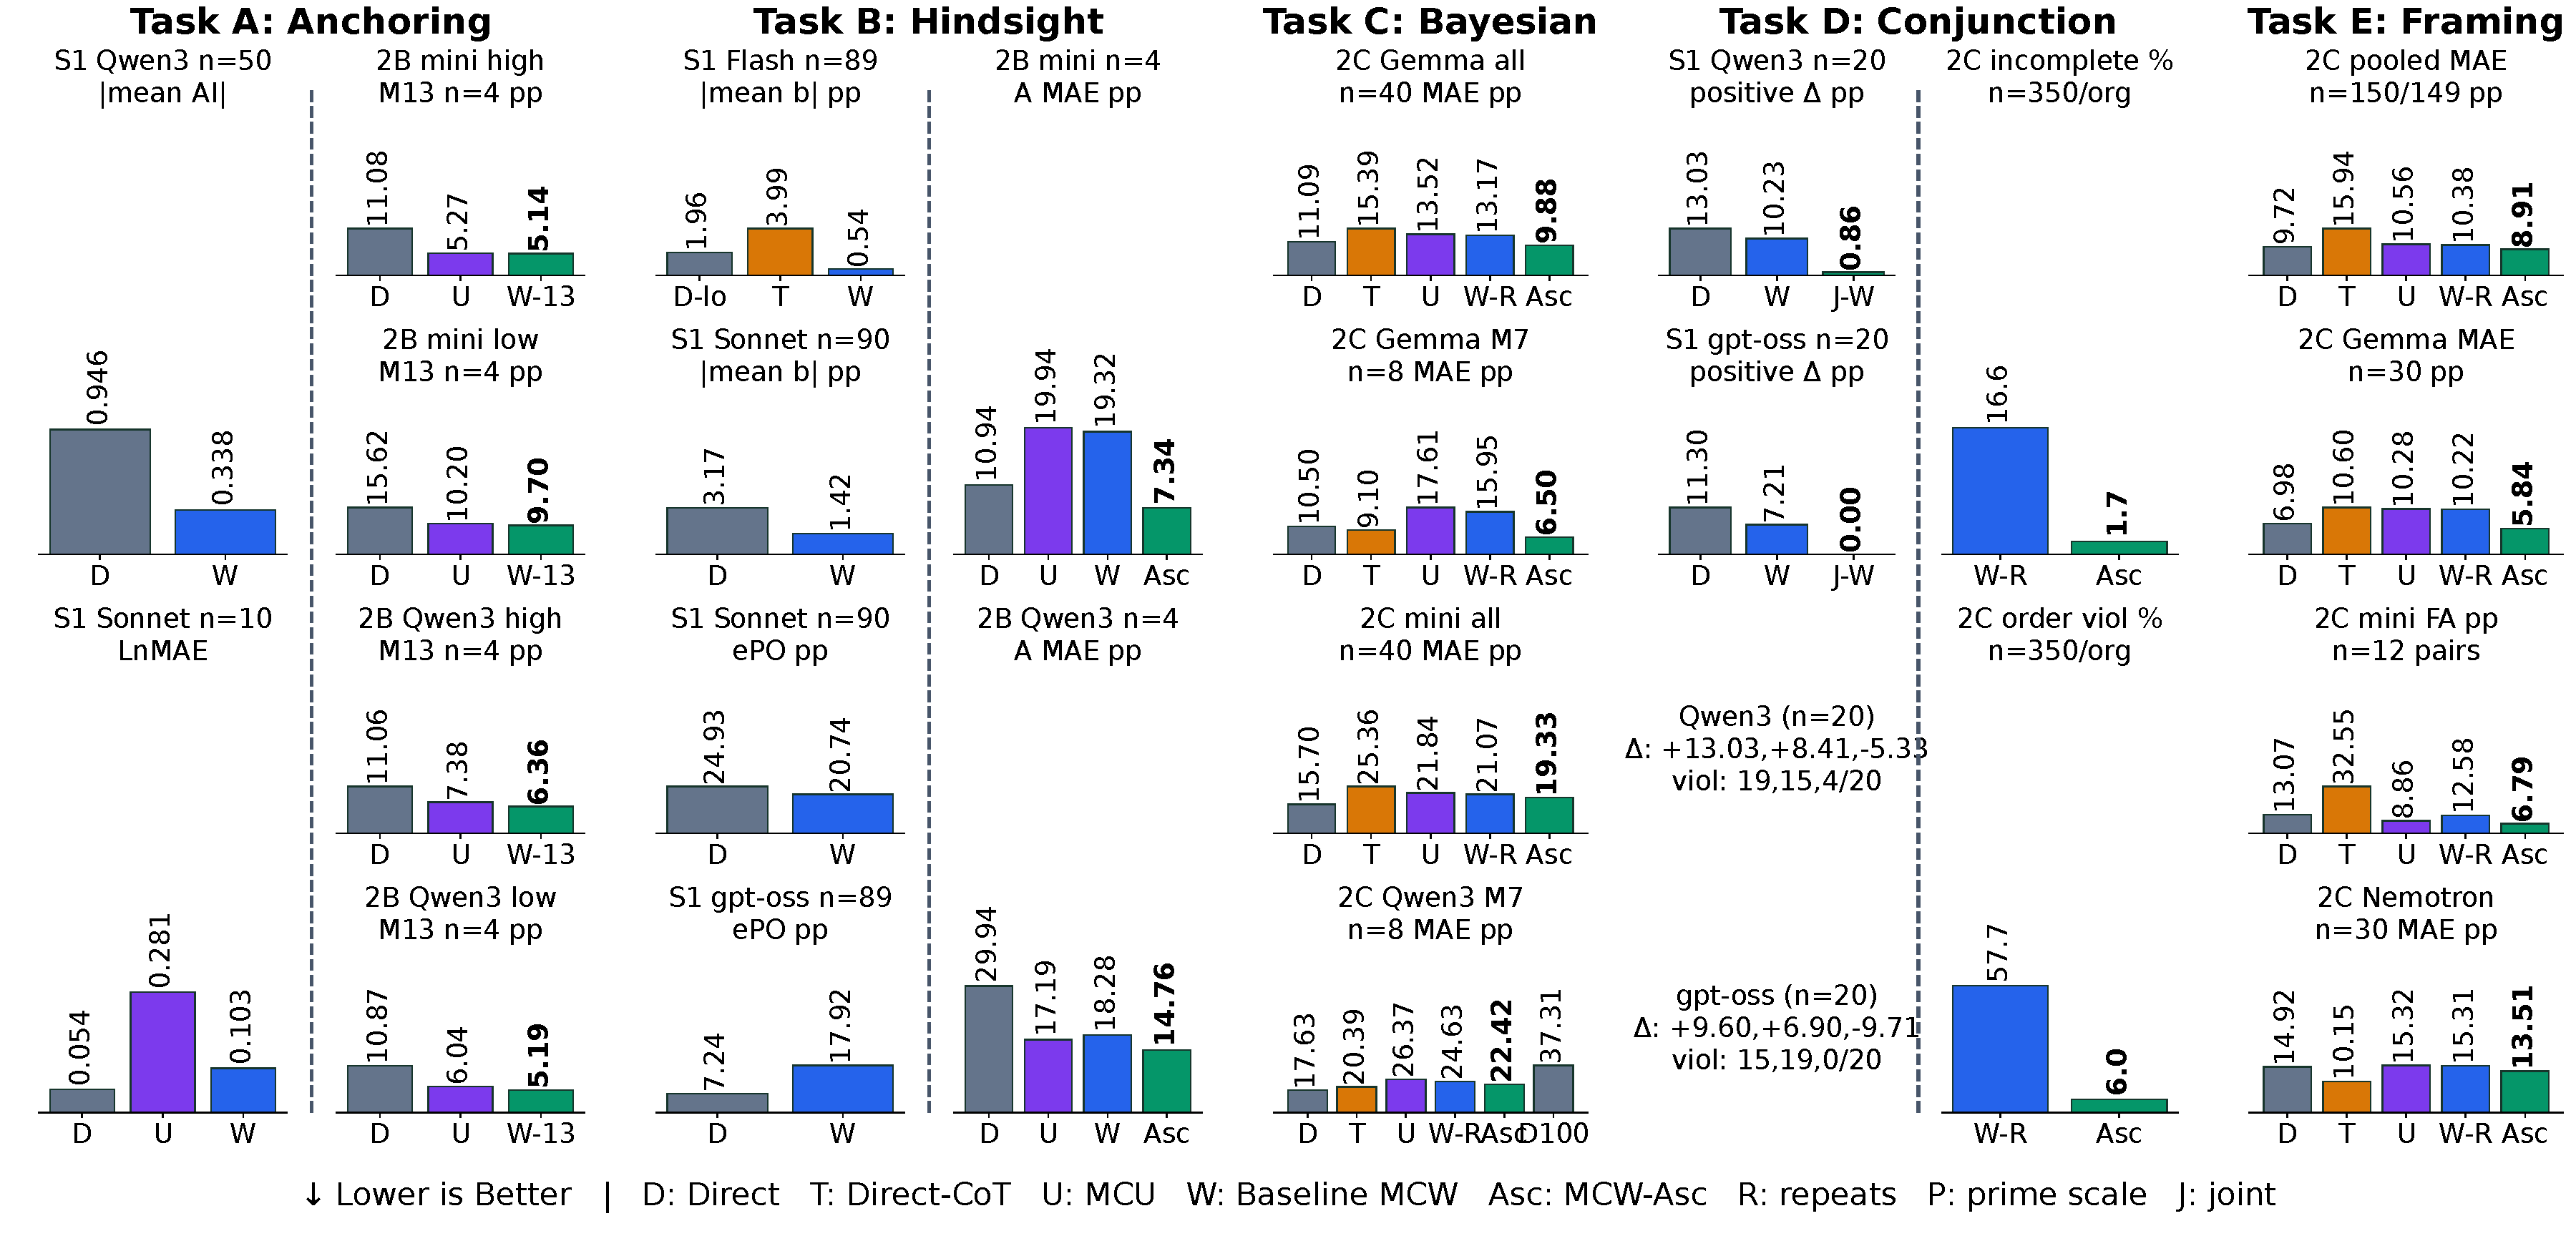
\includegraphics[width=\linewidth,height=.68\textheight,keepaspectratio]{figures/fig_5tasks_mcv_comparison.pdf}\end{center}
Figure 5. Task-\allowbreak{}specific descriptive comparisons across Stage 1 Formal,\allowbreak{} Stage 1 Dev,\allowbreak{} Stage 2B,\allowbreak{} and Stage 2C slices (all panels:\allowbreak{} lower is better). Subpanels retain distinct vertical scales,\allowbreak{} units (\texttt{|mean AI|},\allowbreak{} \texttt{LnMAE},\allowbreak{} \texttt{pp},\allowbreak{} \texttt{\%}),\allowbreak{} and denominators separated by dashed boundaries; missing bars indicate combinations not run in that slice rather than zero or imputed values. Protocol labels map to concrete stage-\allowbreak{}specific arms in \texttt{story\_\allowbreak{}figures\_\allowbreak{}ledger.json}:\allowbreak{} (1) in the Stage 1 Formal Flash hindsight slice (\texttt{D-\allowbreak{}lo /\allowbreak{} T /\allowbreak{} W},\allowbreak{} paired $n=89$,\allowbreak{} $|\text{mean } b|$ in \texttt{pp}),\allowbreak{} the bar plotted under legend slot \texttt{T} (\texttt{Direct-\allowbreak{}CoT}) represents the frozen Flash-\allowbreak{}high direct reasoning-\allowbreak{}budget configuration ($3.99\text{ pp}$,\allowbreak{} contrasted against Flash-\allowbreak{}low direct \texttt{D-\allowbreak{}lo} at $1.96\text{ pp}$ and Flash-\allowbreak{}high multi \texttt{W} at $0.54\text{ pp}$),\allowbreak{} which is a reasoning-\allowbreak{}budget configuration contrast rather than an explicit chain-\allowbreak{}of-\allowbreak{}thought prompt intervention; (2) the bottom two panels in row B (\texttt{Stage 2B A},\allowbreak{} $n=4$/\allowbreak{}arm) are narrative Bayesian prior-\allowbreak{}anchor proxies rather than ProbCOPA hindsight reconstruction trials,\allowbreak{} and the Stage 2C panels in row D (\texttt{incomplete \%} and \texttt{order violation \%},\allowbreak{} $n=350$/\allowbreak{}org) are multi-\allowbreak{}candidate structural format diagnostics rather than conjunction probability trials; (3) every \texttt{MCU} (\texttt{V2}) bar shown here (Stage 1 Dev \texttt{A\_\allowbreak{}ln} $n=10$,\allowbreak{} Stage 2B \texttt{multi\_\allowbreak{}free}/\allowbreak{}\texttt{multi},\allowbreak{} and Stage 2C \texttt{multi\_\allowbreak{}repeat}) is a same-\allowbreak{}generation equal-\allowbreak{}weight readout computed from the corresponding weighted multi-\allowbreak{}candidate output,\allowbreak{} not an independent unweighted prompt arm (prompt-\allowbreak{}level weight elicitation is isolated separately in post-\allowbreak{}cohort Suite P2-\allowbreak{}A,\allowbreak{} Table 5); and (4) \texttt{Baseline MCW} denotes Stage 1 \texttt{ASK\_\allowbreak{}MULTI},\allowbreak{} Stage 2B distinct-\allowbreak{}candidate \texttt{multi\_\allowbreak{}free}/\allowbreak{}\texttt{multi},\allowbreak{} or Stage 2C repeat-\allowbreak{}allowed \texttt{multi\_\allowbreak{}repeat},\allowbreak{} whereas upgraded green bars denote slice-\allowbreak{}specific variants---Stage 1 D joint presentation (\texttt{Joint + MCW}),\allowbreak{} Stage 2B point-\allowbreak{}first ascending without repeat (\texttt{1p5\_\allowbreak{}asc}),\allowbreak{} Stage 2B prime-\allowbreak{}scale distinct multi (\texttt{M=13 multi}),\allowbreak{} or Stage 2C combined point-\allowbreak{}first ascending with repeats (\texttt{1p5\_\allowbreak{}asc\_\allowbreak{}repeat})---not a single uniform protocol across stages.\par\clearpage

% END M:338

% BEGIN M:340 text

\clearpage\begin{center}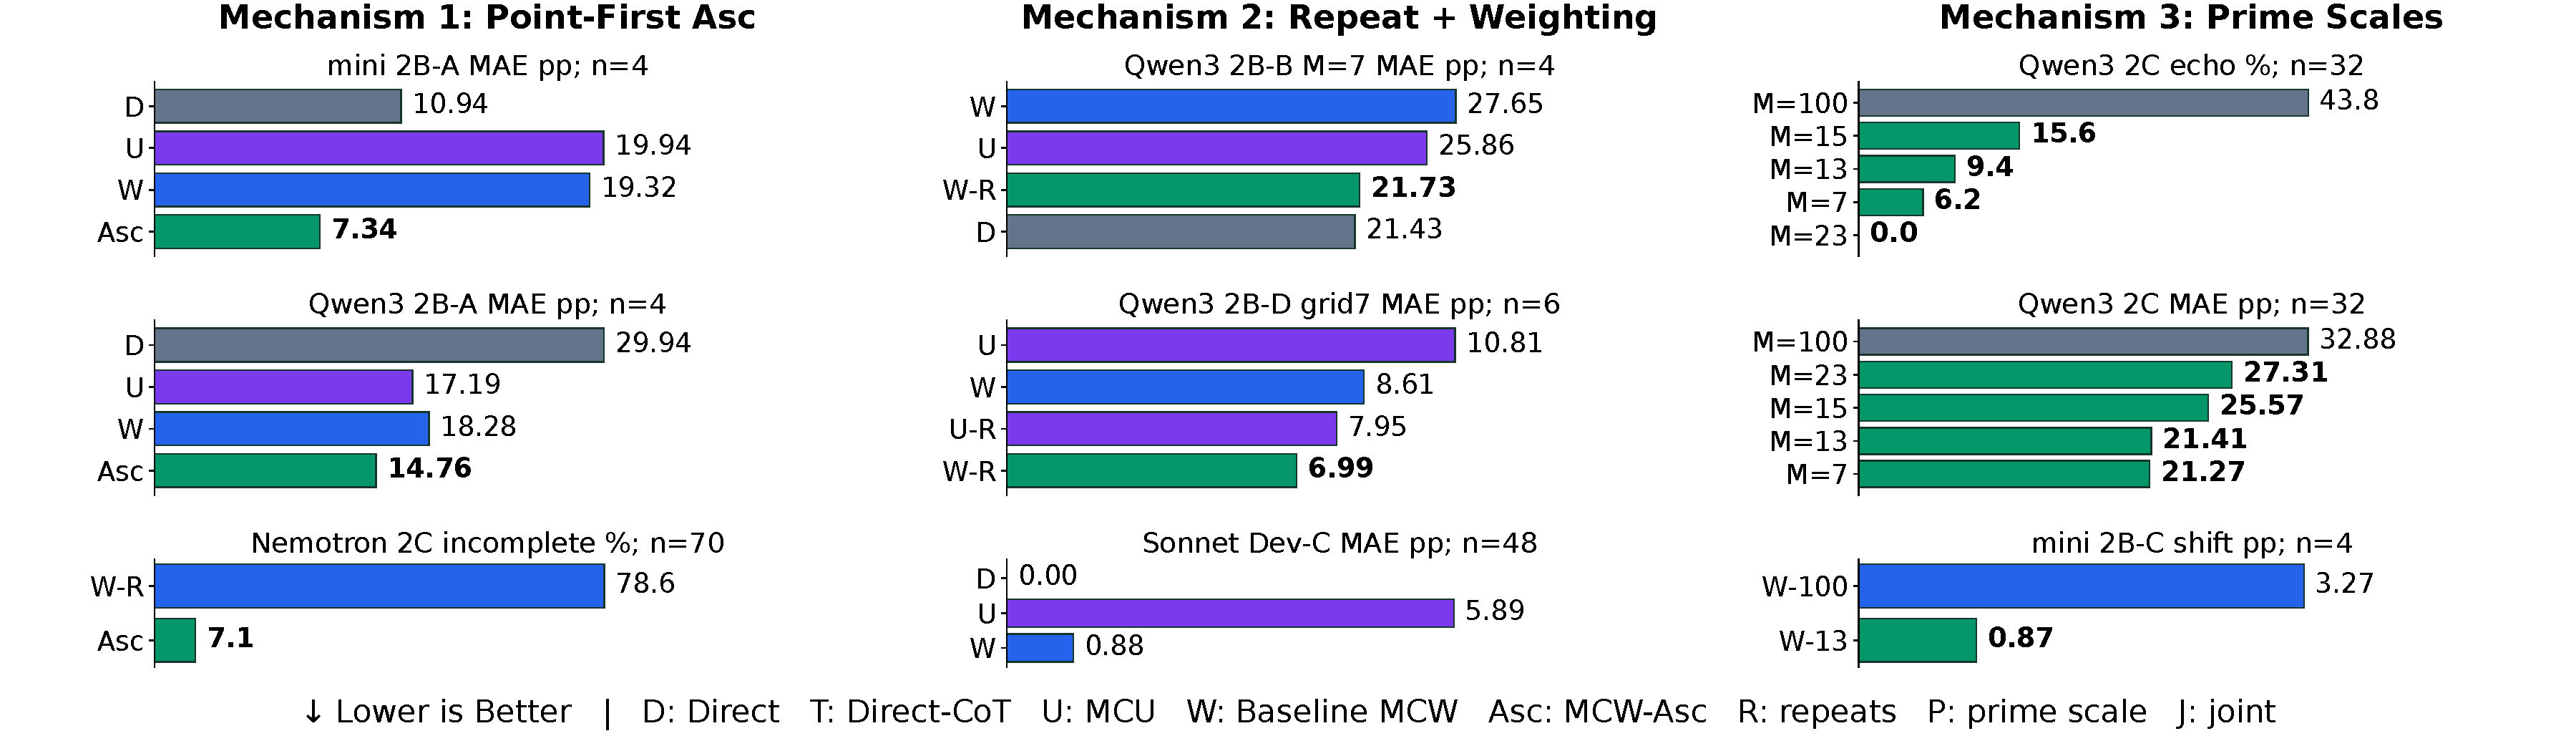
\includegraphics[width=\linewidth,height=.68\textheight,keepaspectratio]{figures/fig_act3_3mechanisms.pdf}\end{center}
Figure 6. Exploratory protocol-\allowbreak{}manipulation comparisons across ordering (left),\allowbreak{} repeat allowance and weighting readouts (middle),\allowbreak{} and non-\allowbreak{}decimal response scales (right; all panels:\allowbreak{} lower is better). The embedded panel banners ``Mechanism 1--3'' are descriptive,\allowbreak{} hypothesis-\allowbreak{}generating groupings of observable prompt manipulations and do not identify internal cognitive,\allowbreak{} attentional,\allowbreak{} or neural causal mechanisms,\allowbreak{} which remain unmeasured hypotheses (Section 6). Each subpanel retains its own stage,\allowbreak{} model,\allowbreak{} sample size ($n=4$ or $6$ in Stage 2B; $n=32$ or $70$ in Stage 2C; $n=48$ in Stage 1 Dev C),\allowbreak{} and native metric (\texttt{MAE pp},\allowbreak{} \texttt{incomplete \%},\allowbreak{} \texttt{echo \%},\allowbreak{} or anchor \texttt{shift pp}),\allowbreak{} without forming a common cross-\allowbreak{}task score. Across all panels,\allowbreak{} \texttt{MCU} (\texttt{V2}) bars are same-\allowbreak{}generation equal-\allowbreak{}weight readouts from weighted multi-\allowbreak{}candidate responses (\texttt{multi\_\allowbreak{}free},\allowbreak{} \texttt{multi},\allowbreak{} \texttt{multi\_\allowbreak{}repeat},\allowbreak{} or Stage 1 Dev \texttt{ASK\_\allowbreak{}MULTI}) rather than separate unweighted prompts; \texttt{MCW-\allowbreak{}Asc} in Stage 2B Block A denotes \texttt{1p5\_\allowbreak{}asc} (distinct candidates),\allowbreak{} whereas only Stage 2C uses the combined \texttt{1p5\_\allowbreak{}asc\_\allowbreak{}repeat} protocol.\par\clearpage

% END M:340

% BEGIN M:342 text

\subsection{Preregistered Post-\allowbreak{}Cohort Formal Verification Suites (P1 and P2)}

% END M:342

% BEGIN M:344 text

\subsubsection{Suite P1:\allowbreak{} Orthogonal PF \ensuremath{\times} ASC and Scale \ensuremath{\times} Cue-\allowbreak{}Format Factorials}\label{sec:5.3.1}

% END M:344

% BEGIN M:346 text

P1 completes 1,\allowbreak{}920/\allowbreak{}1,\allowbreak{}920 terminal units across \texttt{sf:\allowbreak{}qwen3-\allowbreak{}8b},\allowbreak{} \texttt{aistudio:\allowbreak{}gemma-\allowbreak{}4-\allowbreak{}26b-\allowbreak{}a4b-\allowbreak{}it},\allowbreak{} \texttt{nv:\allowbreak{}nemotron-\allowbreak{}3.5-\allowbreak{}super-\allowbreak{}vl-\allowbreak{}120b} and \texttt{xf:\allowbreak{}spark-\allowbreak{}x2.6},\allowbreak{} R=2,\allowbreak{} B=10,\allowbreak{}000,\allowbreak{} seed=20261110,\allowbreak{} with 0\% final missing/\allowbreak{}truncated outcomes. Terminal completion is distinct from first-\allowbreak{}attempt parsing. Block A crosses point-\allowbreak{}first (PF) and ascending order (ASC) in A00/\allowbreak{}A01/\allowbreak{}A10/\allowbreak{}A11:\allowbreak{} 4 models \ensuremath{\times} 4 arms \ensuremath{\times} 72 units = 1,\allowbreak{}152 units. Each arm contains 12 Bayesian clusters (24 units) and 12 paired-\allowbreak{}framing clusters (48 units). A\_\allowbreak{}Bayesian measures MAE (SESOI 1.5 pp); A\_\allowbreak{}Framing measures FrameGap,\allowbreak{} positive/\allowbreak{}negative polarity asymmetry (SESOI 2.0 pp). All six pooled tests have p\_\allowbreak{}Holm=1.0000. Model-\allowbreak{}specific secondary estimates include Gemma Bayesian Delta\_\allowbreak{}A -\allowbreak{}0.76 pp (p=0.0012),\allowbreak{} Nemotron FrameGap Delta\_\allowbreak{}A -\allowbreak{}0.21 pp (p=0.0132),\allowbreak{} both below their SESOIs; Nemotron Bayesian interaction +2.90 pp (p=0.0270); and Qwen FrameGap Delta\_\allowbreak{}A +4.31 pp (p=0.0012).\par

% END M:346

% BEGIN M:348 text

Block B crosses M100/\allowbreak{}M13/\allowbreak{}M15 with pct/\allowbreak{}freq:\allowbreak{} 4 models \ensuremath{\times} 6 cells \ensuremath{\times} 32 units = 768 units,\allowbreak{} using 16 Bayesian clusters. All P1 intervals in Table 4 are \textbf{95\% simultaneous CIs},\allowbreak{} JSON \texttt{ci95\_\allowbreak{}simultaneous},\allowbreak{} constructed by single-\allowbreak{}step Bonferroni percentile bootstrap at alpha/\allowbreak{}(2k),\allowbreak{} with k=3 or 6 within each family. Models are equally weighted; inference resamples paired scenario clusters,\allowbreak{} retaining replicates within their clusters.\par

% END M:348

% BEGIN M:350 text

\textbf{Table 4. P1 pooled primary and selected model-\allowbreak{}specific secondary effects.} Each label binds family,\allowbreak{} endpoint,\allowbreak{} population and contrast to the summary JSON. Delta\_\allowbreak{}P and Delta\_\allowbreak{}A are factorial main effects; interaction is the difference of differences. Delta\_\allowbreak{}13\_\allowbreak{}100\_\allowbreak{}pct/\allowbreak{}freq and Delta\_\allowbreak{}15\_\allowbreak{}100\_\allowbreak{}pct/\allowbreak{}freq compare scales within cue format; DiD compares the scale effect across cue formats. Negative errors favor the first condition.\par

% END M:350

% BEGIN M:352 table

\begingroup\scriptsize\setlength{\tabcolsep}{1.3mm}\setlength{\LTpre}{4pt}\setlength{\LTpost}{6pt}
\begin{longtable}{>{\raggedright\arraybackslash}p{45.541mm}>{\raggedright\arraybackslash}p{20.373mm}>{\raggedright\arraybackslash}p{20.373mm}>{\raggedright\arraybackslash}p{19.175mm}>{\raggedright\arraybackslash}p{36.433mm}>{\raggedright\arraybackslash}p{11.505mm}}
\toprule
Population /\allowbreak{} family & Endpoint & Contrast & Delta (pp) & 95\% simultaneous CI & p\_\allowbreak{}Holm \\
\midrule\endfirsthead
\toprule
Population /\allowbreak{} family & Endpoint & Contrast & Delta (pp) & 95\% simultaneous CI & p\_\allowbreak{}Holm \\
\midrule\endhead
\bottomrule\endfoot
A\_\allowbreak{}Bayesian; four\_\allowbreak{}models\_\allowbreak{}equal & MAE & Delta\_\allowbreak{}P & -\allowbreak{}0.17 & [-\allowbreak{}1.629,\allowbreak{} +1.357] & 1.0000 \\
A\_\allowbreak{}Bayesian; four\_\allowbreak{}models\_\allowbreak{}equal & MAE & Delta\_\allowbreak{}A & +0.51 & [-\allowbreak{}0.751,\allowbreak{} +1.949] & 1.0000 \\
A\_\allowbreak{}Bayesian; four\_\allowbreak{}models\_\allowbreak{}equal & MAE & interaction & -\allowbreak{}0.04 & [-\allowbreak{}2.872,\allowbreak{} +2.173] & 1.0000 \\
A\_\allowbreak{}Bayesian; aistudio:\allowbreak{}gemma-\allowbreak{}4-\allowbreak{}26b-\allowbreak{}a4b-\allowbreak{}it & MAE & Delta\_\allowbreak{}A & -\allowbreak{}0.76 & [-\allowbreak{}1.640,\allowbreak{} -\allowbreak{}0.129] & 0.0012 \\
A\_\allowbreak{}Bayesian; nv:\allowbreak{}nemotron-\allowbreak{}3.5-\allowbreak{}super-\allowbreak{}vl-\allowbreak{}120b & MAE & interaction & +2.90 & [+0.233,\allowbreak{} +6.093] & 0.0270 \\
A\_\allowbreak{}Framing; four\_\allowbreak{}models\_\allowbreak{}equal & FrameGap & Delta\_\allowbreak{}P & +0.93 & [-\allowbreak{}0.801,\allowbreak{} +3.987] & 1.0000 \\
A\_\allowbreak{}Framing; four\_\allowbreak{}models\_\allowbreak{}equal & FrameGap & Delta\_\allowbreak{}A & +0.68 & [-\allowbreak{}1.389,\allowbreak{} +2.213] & 1.0000 \\
A\_\allowbreak{}Framing; four\_\allowbreak{}models\_\allowbreak{}equal & FrameGap & interaction & -\allowbreak{}0.51 & [-\allowbreak{}1.811,\allowbreak{} +0.823] & 1.0000 \\
A\_\allowbreak{}Framing; sf:\allowbreak{}qwen3-\allowbreak{}8b & FrameGap & Delta\_\allowbreak{}A & +4.31 & [+1.216,\allowbreak{} +8.245] & 0.0012 \\
A\_\allowbreak{}Framing; nv:\allowbreak{}nemotron-\allowbreak{}3.5-\allowbreak{}super-\allowbreak{}vl-\allowbreak{}120b & FrameGap & Delta\_\allowbreak{}A & -\allowbreak{}0.21 & [-\allowbreak{}0.452,\allowbreak{} -\allowbreak{}0.029] & 0.0132 \\
B\_\allowbreak{}MAE; four\_\allowbreak{}models\_\allowbreak{}equal & MAE & Delta\_\allowbreak{}13\_\allowbreak{}100\_\allowbreak{}pct & +6.83 & [+4.289,\allowbreak{} +9.232] & 0.0012 \\
B\_\allowbreak{}MAE; four\_\allowbreak{}models\_\allowbreak{}equal & MAE & Delta\_\allowbreak{}15\_\allowbreak{}100\_\allowbreak{}pct & +6.80 & [+4.883,\allowbreak{} +8.826] & 0.0012 \\
B\_\allowbreak{}MAE; four\_\allowbreak{}models\_\allowbreak{}equal & MAE & Delta\_\allowbreak{}13\_\allowbreak{}100\_\allowbreak{}freq & +8.18 & [+5.651,\allowbreak{} +10.528] & 0.0012 \\
B\_\allowbreak{}MAE; four\_\allowbreak{}models\_\allowbreak{}equal & MAE & Delta\_\allowbreak{}15\_\allowbreak{}100\_\allowbreak{}freq & +11.50 & [+7.584,\allowbreak{} +16.066] & 0.0012 \\
B\_\allowbreak{}MAE; four\_\allowbreak{}models\_\allowbreak{}equal & MAE & DiD\_\allowbreak{}13 & +1.34 & [-\allowbreak{}1.527,\allowbreak{} +3.938] & 0.2058 \\
B\_\allowbreak{}MAE; four\_\allowbreak{}models\_\allowbreak{}equal & MAE & DiD\_\allowbreak{}15 & +4.70 & [-\allowbreak{}0.034,\allowbreak{} +10.189] & 0.0180 \\
B\_\allowbreak{}Echo\_\allowbreak{}D2; four\_\allowbreak{}models\_\allowbreak{}equal & Echo\_\allowbreak{}D2 & Delta\_\allowbreak{}13\_\allowbreak{}100\_\allowbreak{}pct & +2.34 & [-\allowbreak{}3.125,\allowbreak{} +9.375] & 1.0000 \\
B\_\allowbreak{}Echo\_\allowbreak{}D2; four\_\allowbreak{}models\_\allowbreak{}equal & Echo\_\allowbreak{}D2 & Delta\_\allowbreak{}15\_\allowbreak{}100\_\allowbreak{}pct & +1.56 & [-\allowbreak{}2.344,\allowbreak{} +5.469] & 1.0000 \\
B\_\allowbreak{}Echo\_\allowbreak{}D2; four\_\allowbreak{}models\_\allowbreak{}equal & Echo\_\allowbreak{}D2 & Delta\_\allowbreak{}13\_\allowbreak{}100\_\allowbreak{}freq & -\allowbreak{}1.56 & [-\allowbreak{}7.812,\allowbreak{} +3.906] & 1.0000 \\
B\_\allowbreak{}Echo\_\allowbreak{}D2; four\_\allowbreak{}models\_\allowbreak{}equal & Echo\_\allowbreak{}D2 & Delta\_\allowbreak{}15\_\allowbreak{}100\_\allowbreak{}freq & +0.78 & [-\allowbreak{}2.344,\allowbreak{} +4.688] & 1.0000 \\
B\_\allowbreak{}Echo\_\allowbreak{}D2; four\_\allowbreak{}models\_\allowbreak{}equal & Echo\_\allowbreak{}D2 & DiD\_\allowbreak{}13 & -\allowbreak{}3.91 & [-\allowbreak{}15.625,\allowbreak{} +5.469] & 1.0000 \\
B\_\allowbreak{}Echo\_\allowbreak{}D2; four\_\allowbreak{}models\_\allowbreak{}equal & Echo\_\allowbreak{}D2 & DiD\_\allowbreak{}15 & -\allowbreak{}0.78 & [-\allowbreak{}6.250,\allowbreak{} +4.688] & 1.0000 \\
B\_\allowbreak{}cand\_\allowbreak{}str\_\allowbreak{}copy\_\allowbreak{}any; four\_\allowbreak{}models\_\allowbreak{}equal & cand\_\allowbreak{}str\_\allowbreak{}copy\_\allowbreak{}any & Delta\_\allowbreak{}13\_\allowbreak{}100\_\allowbreak{}pct & -\allowbreak{}30.47 & [-\allowbreak{}36.201,\allowbreak{} -\allowbreak{}25.000] & 0.0012 \\
B\_\allowbreak{}cand\_\allowbreak{}str\_\allowbreak{}copy\_\allowbreak{}any; four\_\allowbreak{}models\_\allowbreak{}equal & cand\_\allowbreak{}str\_\allowbreak{}copy\_\allowbreak{}any & Delta\_\allowbreak{}15\_\allowbreak{}100\_\allowbreak{}pct & -\allowbreak{}29.69 & [-\allowbreak{}35.938,\allowbreak{} -\allowbreak{}23.438] & 0.0012 \\
B\_\allowbreak{}cand\_\allowbreak{}str\_\allowbreak{}copy\_\allowbreak{}any; four\_\allowbreak{}models\_\allowbreak{}equal & cand\_\allowbreak{}str\_\allowbreak{}copy\_\allowbreak{}any & Delta\_\allowbreak{}13\_\allowbreak{}100\_\allowbreak{}freq & -\allowbreak{}5.47 & [-\allowbreak{}13.281,\allowbreak{} -\allowbreak{}0.781] & 0.0116 \\
B\_\allowbreak{}cand\_\allowbreak{}str\_\allowbreak{}copy\_\allowbreak{}any; four\_\allowbreak{}models\_\allowbreak{}equal & cand\_\allowbreak{}str\_\allowbreak{}copy\_\allowbreak{}any & Delta\_\allowbreak{}15\_\allowbreak{}100\_\allowbreak{}freq & -\allowbreak{}5.47 & [-\allowbreak{}13.281,\allowbreak{} -\allowbreak{}0.781] & 0.0116 \\
B\_\allowbreak{}cand\_\allowbreak{}str\_\allowbreak{}copy\_\allowbreak{}any; four\_\allowbreak{}models\_\allowbreak{}equal & cand\_\allowbreak{}str\_\allowbreak{}copy\_\allowbreak{}any & DiD\_\allowbreak{}13 & +25.00 & [+17.188,\allowbreak{} +32.031] & 0.0012 \\
B\_\allowbreak{}cand\_\allowbreak{}str\_\allowbreak{}copy\_\allowbreak{}any; four\_\allowbreak{}models\_\allowbreak{}equal & cand\_\allowbreak{}str\_\allowbreak{}copy\_\allowbreak{}any & DiD\_\allowbreak{}15 & +24.22 & [+15.625,\allowbreak{} +32.031] & 0.0012 \\
\end{longtable}
\endgroup

% END M:352

% BEGIN M:383 text

The pct operational string-\allowbreak{}match rate is 40/\allowbreak{}128 = 31.25\% at M100,\allowbreak{} 1/\allowbreak{}128 = 0.78\% at M13 and 2/\allowbreak{}128 = 1.56\% at M15:\allowbreak{} reductions -\allowbreak{}30.47 and -\allowbreak{}29.69 pp,\allowbreak{} with nonzero residual matching. Under freq it is 7/\allowbreak{}128 = 5.47\% at M100 and 0/\allowbreak{}128 = 0.00\% at both smaller scales (difference -\allowbreak{}5.47 pp,\allowbreak{} p\_\allowbreak{}Holm=0.0116). The minimum formal freq cue integer is 22 > 15:\allowbreak{} legal raw outputs [0,\allowbreak{}M] structurally preclude matching at M13/\allowbreak{}M15. Thus the result is a large reduction in operational string matching,\allowbreak{} not direct evidence of a copying mechanism. The DiDs are +25.00 and +24.22 pp. In contrast,\allowbreak{} unified percentage-\allowbreak{}tolerance B\_\allowbreak{}Echo\_\allowbreak{}D2 effects range -\allowbreak{}3.91 to +2.34 pp,\allowbreak{} all p\_\allowbreak{}Holm=1.0000. Bayesian B\_\allowbreak{}MAE rises +6.83 /\allowbreak{} +6.80 pp in pct and +8.18 /\allowbreak{} +11.50 pp in freq,\allowbreak{} all p\_\allowbreak{}Holm=0.0012. The MAE DiD\_\allowbreak{}13 is +1.34 pp; DiD\_\allowbreak{}15 is +4.70 pp with simultaneous CI [-\allowbreak{}0.03,\allowbreak{} +10.19] and p\_\allowbreak{}Holm=0.0180. The interval uses fixed Bonferroni tail alpha/\allowbreak{}(2k),\allowbreak{} k=6 (\texttt{analyze\_\allowbreak{}p1\_\allowbreak{}factorial.py},\allowbreak{} line 31); Holm uses step-\allowbreak{}down rank correction of p-\allowbreak{}values. They are different constructions and need not agree about zero inclusion.\par

% END M:383

P1 Block B operational string-\allowbreak{}matching counts across response scales and cue formats (identical to Appendix I.10).\par

% BEGIN M:464 table

\begingroup\scriptsize\setlength{\tabcolsep}{1.3mm}\setlength{\LTpre}{4pt}\setlength{\LTpost}{6pt}
\begin{longtable}{>{\raggedright\arraybackslash}p{57.902mm}>{\raggedright\arraybackslash}p{20.140mm}>{\raggedright\arraybackslash}p{60.419mm}>{\raggedright\arraybackslash}p{20.140mm}}
\toprule
Measure & Cell & Matched /\allowbreak{} valid & Rate \\
\midrule\endfirsthead
\toprule
Measure & Cell & Matched /\allowbreak{} valid & Rate \\
\midrule\endhead
\bottomrule\endfoot
P1 operational matching & M100\_\allowbreak{}pct & 40/\allowbreak{}128 & 31.25\% \\
P1 operational matching & M13\_\allowbreak{}pct & 1/\allowbreak{}128 & 0.78\% \\
P1 operational matching & M15\_\allowbreak{}pct & 2/\allowbreak{}128 & 1.56\% \\
P1 operational matching & M100\_\allowbreak{}freq & 7/\allowbreak{}128 & 5.47\% \\
P1 operational matching & M13\_\allowbreak{}freq & 0/\allowbreak{}128 & 0.00\% \\
P1 operational matching & M15\_\allowbreak{}freq & 0/\allowbreak{}128 & 0.00\% \\
\end{longtable}
\endgroup

% END M:464

% BEGIN M:385 text

\subsubsection{Suite P2:\allowbreak{} Prompt-\allowbreak{}Level Weight Ablation and Three-\allowbreak{}Option Normalization versus Call Decoupling}\label{sec:5.3.2}

% END M:385

% BEGIN M:387 text

P2 has 2,\allowbreak{}560/\allowbreak{}2,\allowbreak{}560 planned/\allowbreak{}admitted terminal calls and 2,\allowbreak{}048/\allowbreak{}2,\allowbreak{}048 complete evaluation units. First-\allowbreak{}attempt parsing is 2,\allowbreak{}556/\allowbreak{}2,\allowbreak{}560 = 99.84\%; final missing/\allowbreak{}truncated is 0\%. The same four API models are equally weighted. R=2,\allowbreak{} B=10,\allowbreak{}000,\allowbreak{} seed=20261110. P2-\allowbreak{}A has 1,\allowbreak{}280 units,\allowbreak{} with 12 Bayesian and 8 paired-\allowbreak{}framing clusters per model. E0\_\allowbreak{}direct returns one estimate; E1\_\allowbreak{}generic\_\allowbreak{}cot requests generic arithmetic decomposition; E2\_\allowbreak{}unweighted\_\allowbreak{}mcv requests candidates without weights; E3\_\allowbreak{}weighted\_\allowbreak{}mcv requests candidates with weights. Delta\_\allowbreak{}elicit = E3(M\_\allowbreak{}W) \ensuremath{-} E2(M\_\allowbreak{}U) is the prompt-\allowbreak{}level intervention; delta\_\allowbreak{}readout = E3(M\_\allowbreak{}W) \ensuremath{-} E3(M\_\allowbreak{}U) holds generation fixed. Direct-\allowbreak{}CoT here is E1\_\allowbreak{}generic\_\allowbreak{}cot,\allowbreak{} which differs from the Stage 2C posterior-\allowbreak{}focus scaffold.\par

% END M:387

% BEGIN M:389 text

\textbf{Table 5. P2 complete pooled arm means,\allowbreak{} primary effects,\allowbreak{} same-\allowbreak{}generation readouts and P2-\allowbreak{}B arm metrics.} The four panels are identically ordered in both languages and Appendix I. \texttt{95\% marginal CI} is JSON \texttt{ci95\_\allowbreak{}raw}; \texttt{95\% simultaneous CI} is JSON \texttt{ci95\_\allowbreak{}simultaneous},\allowbreak{} a single-\allowbreak{}step Bonferroni percentile bootstrap at alpha/\allowbreak{}(2k) (\texttt{analyze\_\allowbreak{}p2\_\allowbreak{}supplemental.py},\allowbreak{} line 47). P2-\allowbreak{}A k=3 per endpoint and P2-\allowbreak{}B k=6 over the two primary endpoints. Values are pp unless percentages or ratios are indicated; C2-\allowbreak{}C1's simultaneous upper endpoint remains -\allowbreak{}0.006 rather than rounding to zero.\par

% END M:389

% BEGIN M:391 table

\begingroup\scriptsize\setlength{\tabcolsep}{1.3mm}\setlength{\LTpre}{4pt}\setlength{\LTpost}{6pt}
\begin{longtable}{>{\raggedright\arraybackslash}p{19.810mm}>{\raggedright\arraybackslash}p{22.286mm}>{\raggedright\arraybackslash}p{34.667mm}>{\raggedright\arraybackslash}p{42.095mm}>{\raggedright\arraybackslash}p{37.143mm}}
\toprule
Endpoint & E0\_\allowbreak{}direct & E1\_\allowbreak{}generic\_\allowbreak{}cot & E2\_\allowbreak{}unweighted\_\allowbreak{}mcv & E3\_\allowbreak{}weighted\_\allowbreak{}mcv \\
\midrule\endfirsthead
\toprule
Endpoint & E0\_\allowbreak{}direct & E1\_\allowbreak{}generic\_\allowbreak{}cot & E2\_\allowbreak{}unweighted\_\allowbreak{}mcv & E3\_\allowbreak{}weighted\_\allowbreak{}mcv \\
\midrule\endhead
\bottomrule\endfoot
bayes\_\allowbreak{}MAE & 5.05 & 0.76 & 7.75 & 10.51 \\
frame\_\allowbreak{}MAE & 7.89 & 0.00 & 0.08 & 2.13 \\
frame\_\allowbreak{}FrameGap & 9.22 & 0.00 & 0.16 & 4.04 \\
\end{longtable}
\endgroup

% END M:391

% BEGIN M:397 table

\begingroup\scriptsize\setlength{\tabcolsep}{1.3mm}\setlength{\LTpre}{4pt}\setlength{\LTpost}{6pt}
\begin{longtable}{>{\raggedright\arraybackslash}p{33.708mm}>{\raggedright\arraybackslash}p{14.193mm}>{\raggedright\arraybackslash}p{14.193mm}>{\raggedright\arraybackslash}p{17.741mm}>{\raggedright\arraybackslash}p{26.612mm}>{\raggedright\arraybackslash}p{33.708mm}>{\raggedright\arraybackslash}p{10.645mm}}
\toprule
Population /\allowbreak{} family & Endpoint & Contrast & Delta (pp) & 95\% marginal CI & 95\% simultaneous CI & p\_\allowbreak{}Holm \\
\midrule\endfirsthead
\toprule
Population /\allowbreak{} family & Endpoint & Contrast & Delta (pp) & 95\% marginal CI & 95\% simultaneous CI & p\_\allowbreak{}Holm \\
\midrule\endhead
\bottomrule\endfoot
P2-\allowbreak{}A & bayes\_\allowbreak{}MAE & delta\_\allowbreak{}elicit & +2.75 & [+1.75,\allowbreak{} +3.79] & [+1.539,\allowbreak{} +4.031] & 0.0006 \\
P2-\allowbreak{}A & bayes\_\allowbreak{}MAE & delta\_\allowbreak{}vs\_\allowbreak{}cot & +9.74 & [+8.21,\allowbreak{} +11.43] & [+7.943,\allowbreak{} +11.846] & 0.0006 \\
P2-\allowbreak{}A & bayes\_\allowbreak{}MAE & delta\_\allowbreak{}vs\_\allowbreak{}direct & +5.46 & [+3.91,\allowbreak{} +7.11] & [+3.599,\allowbreak{} +7.512] & 0.0006 \\
P2-\allowbreak{}A & frame\_\allowbreak{}MAE & delta\_\allowbreak{}elicit & +2.05 & [+0.48,\allowbreak{} +4.17] & [+0.291,\allowbreak{} +4.785] & 0.0006 \\
P2-\allowbreak{}A & frame\_\allowbreak{}MAE & delta\_\allowbreak{}vs\_\allowbreak{}cot & +2.13 & [+0.56,\allowbreak{} +4.23] & [+0.389,\allowbreak{} +4.863] & 0.0006 \\
P2-\allowbreak{}A & frame\_\allowbreak{}MAE & delta\_\allowbreak{}vs\_\allowbreak{}direct & -\allowbreak{}5.76 & [-\allowbreak{}8.24,\allowbreak{} -\allowbreak{}3.76] & [-\allowbreak{}8.920,\allowbreak{} -\allowbreak{}3.500] & 0.0006 \\
P2-\allowbreak{}A & frame\_\allowbreak{}FrameGap & delta\_\allowbreak{}elicit & +3.88 & [+0.67,\allowbreak{} +8.20] & [+0.318,\allowbreak{} +9.508] & 0.0036 \\
P2-\allowbreak{}A & frame\_\allowbreak{}FrameGap & delta\_\allowbreak{}vs\_\allowbreak{}cot & +4.04 & [+0.85,\allowbreak{} +8.32] & [+0.497,\allowbreak{} +9.617] & 0.0006 \\
P2-\allowbreak{}A & frame\_\allowbreak{}FrameGap & delta\_\allowbreak{}vs\_\allowbreak{}direct & -\allowbreak{}5.18 & [-\allowbreak{}9.55,\allowbreak{} -\allowbreak{}0.25] & [-\allowbreak{}10.426,\allowbreak{} +0.906] & 0.0390 \\
P2-\allowbreak{}B; category 2 & MAE\_\allowbreak{}norm & C2-\allowbreak{}C1 & -\allowbreak{}1.27 & [-\allowbreak{}2.35,\allowbreak{} -\allowbreak{}0.33] & [-\allowbreak{}2.804,\allowbreak{} -\allowbreak{}0.006] & 0.0410 \\
P2-\allowbreak{}B; category 2 & Acc\_\allowbreak{}argmax & C2-\allowbreak{}C1 & +3.91 & [-\allowbreak{}1.95,\allowbreak{} +9.38] & [-\allowbreak{}3.906,\allowbreak{} +10.938] & 0.8455 \\
P2-\allowbreak{}B; category 2 & MAE\_\allowbreak{}norm & C3-\allowbreak{}C1 & -\allowbreak{}1.71 & [-\allowbreak{}2.76,\allowbreak{} -\allowbreak{}0.75] & [-\allowbreak{}3.158,\allowbreak{} -\allowbreak{}0.451] & 0.0012 \\
P2-\allowbreak{}B; category 2 & Acc\_\allowbreak{}argmax & C3-\allowbreak{}C1 & +2.34 & [-\allowbreak{}4.30,\allowbreak{} +8.98] & [-\allowbreak{}6.250,\allowbreak{} +11.719] & 1.0000 \\
P2-\allowbreak{}B; category 3 & MAE\_\allowbreak{}norm & C3-\allowbreak{}C2 & -\allowbreak{}0.44 & [-\allowbreak{}1.37,\allowbreak{} +0.46] & [-\allowbreak{}1.722,\allowbreak{} +0.724] & 1.0000 \\
P2-\allowbreak{}B; category 3 & Acc\_\allowbreak{}argmax & C3-\allowbreak{}C2 & -\allowbreak{}1.56 & [-\allowbreak{}7.03,\allowbreak{} +3.91] & [-\allowbreak{}8.594,\allowbreak{} +5.469] & 1.0000 \\
\end{longtable}
\endgroup

% END M:397

% BEGIN M:415 table

\begingroup\scriptsize\setlength{\tabcolsep}{1.3mm}\setlength{\LTpre}{4pt}\setlength{\LTpost}{6pt}
\begin{longtable}{>{\raggedright\arraybackslash}p{16.147mm}>{\raggedright\arraybackslash}p{12.111mm}>{\raggedright\arraybackslash}p{12.111mm}>{\raggedright\arraybackslash}p{16.147mm}>{\raggedright\arraybackslash}p{36.332mm}>{\raggedright\arraybackslash}p{60.553mm}}
\toprule
Endpoint & E3 M\_\allowbreak{}W & E3 M\_\allowbreak{}U & E3 Top-\allowbreak{}1 & delta\_\allowbreak{}readout (pp) & elicit/\allowbreak{}readout magnitude ratio \\
\midrule\endfirsthead
\toprule
Endpoint & E3 M\_\allowbreak{}W & E3 M\_\allowbreak{}U & E3 Top-\allowbreak{}1 & delta\_\allowbreak{}readout (pp) & elicit/\allowbreak{}readout magnitude ratio \\
\midrule\endhead
\bottomrule\endfoot
bayes\_\allowbreak{}MAE & 10.51 & 10.56 & 10.63 & -\allowbreak{}0.052 & 52.98 \\
frame\_\allowbreak{}MAE & 2.13 & 2.18 & 2.39 & -\allowbreak{}0.049 & 41.63 \\
frame\_\allowbreak{}FrameGap & 4.04 & 4.11 & 4.28 & -\allowbreak{}0.067 & 57.74 \\
\end{longtable}
\endgroup

% END M:415

% BEGIN M:421 table

\begingroup\scriptsize\setlength{\tabcolsep}{1.3mm}\setlength{\LTpre}{4pt}\setlength{\LTpost}{6pt}
\begin{longtable}{>{\raggedright\arraybackslash}p{35.301mm}>{\raggedright\arraybackslash}p{20.539mm}>{\raggedright\arraybackslash}p{17.972mm}>{\raggedright\arraybackslash}p{12.837mm}>{\raggedright\arraybackslash}p{35.943mm}>{\raggedright\arraybackslash}p{30.808mm}}
\toprule
Arm (m\_\allowbreak{}w) & MAE\_\allowbreak{}norm & MAE\_\allowbreak{}raw & S (\%) & Acc\_\allowbreak{}argmax (\%) & Tie rate (\%) \\
\midrule\endfirsthead
\toprule
Arm (m\_\allowbreak{}w) & MAE\_\allowbreak{}norm & MAE\_\allowbreak{}raw & S (\%) & Acc\_\allowbreak{}argmax (\%) & Tie rate (\%) \\
\midrule\endhead
\bottomrule\endfoot
C1\_\allowbreak{}joint\_\allowbreak{}constrained & 8.67 & 9.05 & 102.58 & 77.73 & 1.95 \\
C2\_\allowbreak{}joint\_\allowbreak{}unconstrained & 7.40 & 7.63 & 101.11 & 81.64 & 1.95 \\
C3\_\allowbreak{}separate\_\allowbreak{}unconstrained & 6.96 & 8.44 & 100.30 & 80.08 & 2.73 \\
\end{longtable}
\endgroup

% END M:421

% BEGIN M:427 text

The weight-\allowbreak{}elicitation effects are +2.75 pp [marginal 95\% CI +1.75,\allowbreak{} +3.79],\allowbreak{} +2.05 [+0.48,\allowbreak{} +4.17],\allowbreak{} and +3.88 [+0.67,\allowbreak{} +8.20],\allowbreak{} p\_\allowbreak{}Holm=0.0006 /\allowbreak{} 0.0006 /\allowbreak{} 0.0036. Their same-\allowbreak{}generation counterparts are -\allowbreak{}0.052 /\allowbreak{} -\allowbreak{}0.049 /\allowbreak{} -\allowbreak{}0.067 pp,\allowbreak{} approximately 42\ensuremath{\times}--58\ensuremath{\times} smaller in magnitude. Generic arithmetic CoT errors are 0.00--0.76 pp. Among nine improvement tests,\allowbreak{} only frame\_\allowbreak{}MAE E3 \ensuremath{-} Direct passes the improvement gate:\allowbreak{} -\allowbreak{}5.76 pp,\allowbreak{} marginal CI [-\allowbreak{}8.24,\allowbreak{} -\allowbreak{}3.76],\allowbreak{} p\_\allowbreak{}Holm=0.0006. This is driven largely by Gemma-\allowbreak{}4-\allowbreak{}26B (-\allowbreak{}31.50 pp); leaving one model out yields [-\allowbreak{}10.23,\allowbreak{} +2.82] pp. Bayesian E3 \ensuremath{-} Direct increases error +5.46 pp; FrameGap decreases -\allowbreak{}5.18 pp but fails the full improvement gate. Prompt effects and same-\allowbreak{}generation aggregation should therefore be reported separately.\par

% END M:427

% BEGIN M:429 text

P2-\allowbreak{}B's 1,\allowbreak{}280 planned/\allowbreak{}admitted calls yield 768 evaluation units (16 clusters per model). The three options are mutually exclusive and exhaustive. C1\_\allowbreak{}joint\_\allowbreak{}constrained asks for a joint response summing to 100\%; C2\_\allowbreak{}joint\_\allowbreak{}unconstrained removes that generation constraint and normalizes afterward; C3\_\allowbreak{}separate\_\allowbreak{}unconstrained elicits each option in separate calls and then normalizes. The confirmatory readout is M\_\allowbreak{}W. Normalization rescales by the raw sum S; this does not imply the raw outputs themselves sum to 100\%.\par

% END M:429

% BEGIN M:431 text

C2 \ensuremath{-} C1 improves MAE\_\allowbreak{}norm by -\allowbreak{}1.27 pp (marginal CI [-\allowbreak{}2.35,\allowbreak{} -\allowbreak{}0.33]; simultaneous [-\allowbreak{}2.804,\allowbreak{} -\allowbreak{}0.006]; p\_\allowbreak{}Holm=0.0410),\allowbreak{} with leave-\allowbreak{}one-\allowbreak{}model-\allowbreak{}out range [-\allowbreak{}2.11,\allowbreak{} -\allowbreak{}0.57] pp. Acc\_\allowbreak{}argmax increases +3.91 pp,\allowbreak{} p\_\allowbreak{}Holm=0.8455:\allowbreak{} category 2,\allowbreak{} a local error improvement. C3 \ensuremath{-} C1 improves MAE\_\allowbreak{}norm -\allowbreak{}1.71 pp (marginal [-\allowbreak{}2.76,\allowbreak{} -\allowbreak{}0.75]; simultaneous [-\allowbreak{}3.16,\allowbreak{} -\allowbreak{}0.45]; p\_\allowbreak{}Holm=0.0012),\allowbreak{} but accuracy +2.34 pp has p\_\allowbreak{}Holm=1.0000:\allowbreak{} category 2. C3 \ensuremath{-} C2 is -\allowbreak{}0.44 pp (marginal [-\allowbreak{}1.37,\allowbreak{} +0.46]; simultaneous [-\allowbreak{}1.72,\allowbreak{} +0.72]; p\_\allowbreak{}Holm=1.0000),\allowbreak{} accuracy -\allowbreak{}1.56 pp,\allowbreak{} p\_\allowbreak{}Holm=1.0000:\allowbreak{} category 3,\allowbreak{} no detected additional benefit. This is neither equivalence nor noninferiority. The category rule requires joint evidence for normalized error and argmax accuracy for category 1; no contrast meets it.\par

% END M:431

% BEGIN M:433 text

\section{Discussion and Synthesis}

% END M:433

% BEGIN M:435 text

The Three-\allowbreak{}Class Structural Behavioral Spectrum is a descriptive organization across nine model families and ten reasoning-\allowbreak{}budget configurations (Flash low/\allowbreak{}high count separately). It is not a causal law of architecture,\allowbreak{} training or scale. Stage 1 CLI settings and later API endpoints have distinct provenance and cannot be assumed exchangeable.\par

% END M:435

% BEGIN M:437 text

\textbf{Class I:\allowbreak{} Non-\allowbreak{}Thinking Compact \& Open-\allowbreak{}Weight Models.} Qwen3-\allowbreak{}8B,\allowbreak{} GPT-\allowbreak{}4o-\allowbreak{}mini,\allowbreak{} Gemma-\allowbreak{}4-\allowbreak{}26B-\allowbreak{}A4B-\allowbreak{}IT,\allowbreak{} Nemotron-\allowbreak{}3.5-\allowbreak{}Super-\allowbreak{}VL-\allowbreak{}120B and spark-\allowbreak{}x2.6 show heterogeneous sensitivity to protocol organization. The class includes a large MoE and should not be read as a parameter-\allowbreak{}size threshold. The Nemotron 78.6\% \ensuremath{\rightarrow} 7.1\% collapse comparison is \texttt{multi\_\allowbreak{}repeat} \ensuremath{\rightarrow} \texttt{1p5\_\allowbreak{}asc\_\allowbreak{}repeat}. Its posterior-\allowbreak{}focus errors (10.15 pp framing /\allowbreak{} 16.73 pp Bayesian) and Qwen's \texttt{single} framing error (12.98 pp) are counterexamples to universal Upgraded MCW-\allowbreak{}Asc superiority. Stage 2C pooled framing benefits do not imply P1 isolated PF or ASC effects,\allowbreak{} which largely fail their pooled gates.\par

% END M:437

% BEGIN M:439 text

\textbf{Class II:\allowbreak{} Explicit Reasoning Configurations.} Gemini-\allowbreak{}3.8-\allowbreak{}Flash high versus low and gpt-\allowbreak{}oss-\allowbreak{}120b show that arithmetic performance and contextual susceptibility differ. gpt-\allowbreak{}oss-\allowbreak{}120b's B4 post-\allowbreak{}outcome confirmation change is +10.68 pp; C4 is +0.19 pp and does not license the same practical claim. Flash B1 uses all n=90 items:\allowbreak{} high -\allowbreak{}3.97 versus low -\allowbreak{}1.94 pp. B3 uses the paired n=89 subset:\allowbreak{} high -\allowbreak{}3.99 \ensuremath{\rightarrow} +0.54 pp,\allowbreak{} low -\allowbreak{}1.96 \ensuremath{\rightarrow} -\allowbreak{}0.32 pp. These denominators and estimands should not be substituted. Attention/\allowbreak{}working-\allowbreak{}memory competition or motivated self-\allowbreak{}rationalization could explain some pattern differences,\allowbreak{} but each remains a hypothesis without internal measurement or a discriminating intervention.\par

% END M:439

% BEGIN M:441 text

\textbf{Class III:\allowbreak{} Frontier Commercial Flagships.} Claude Sonnet 5.5 and codex use frozen medium settings; server-\allowbreak{}side internal reasoning is unobservable. Their Stage 1 Dev C MCW errors are 0.88 /\allowbreak{} 0.0001 pp versus MCU 5.89 /\allowbreak{} 1.49 pp. Arithmetic ceilings coexist with Sonnet B3 +1.75 pp,\allowbreak{} B4 -\allowbreak{}4.19 pp and D2 = +2.30 pp,\allowbreak{} alongside codex D2 = +2.46 pp contextual effects. Medium settings must not be interpreted as evidence about absence of internal reasoning.\par

% END M:441

% BEGIN M:443 table

Table 6. Conditional protocol recommendations and evidence boundaries across task structures.\par
\begingroup\scriptsize\setlength{\tabcolsep}{1.3mm}\setlength{\LTpre}{4pt}\setlength{\LTpost}{6pt}
\begin{longtable}{>{\raggedright\arraybackslash}p{45.805mm}>{\raggedright\arraybackslash}p{51.091mm}>{\raggedright\arraybackslash}p{64.304mm}}
\toprule
Task structure & Conditional protocol recommendation & Evidence boundary \\
\midrule\endfirsthead
\toprule
Task structure & Conditional protocol recommendation & Evidence boundary \\
\midrule\endhead
\bottomrule\endfoot
Structured closed arithmetic near ceiling & Compare Direct and short Direct-\allowbreak{}CoT first & Extra candidates/\allowbreak{}weights can increase error; validate the actual endpoint \\
Compact/\allowbreak{}open-\allowbreak{}weight narrative estimates with format failures & Test Upgraded MCW-\allowbreak{}Asc alongside Direct and posterior-\allowbreak{}focus & Organization can repair format; model-\allowbreak{}specific counterexamples remain \\
Positive/\allowbreak{}negative attribute framing & Select using objective MAE and FrameGap separately & Lower asymmetry need not imply lower normative error \\
Hindsight,\allowbreak{} irrelevant anchors,\allowbreak{} status/\allowbreak{}default/\allowbreak{}advice & Retain signed shifts and source-\allowbreak{}specific outcomes & No protocol has uniform debiasing support \\
Three exhaustive mutually exclusive options & C2 single unconstrained generation plus post-\allowbreak{}hoc normalization is a local MAE\_\allowbreak{}norm option & Category 2; accuracy improvement unconfirmed; separate calls add no detected benefit over C2 \\
\end{longtable}
\endgroup

% END M:443

% BEGIN M:451 text

A fixed three-\allowbreak{}candidate K\_\allowbreak{}opt=3 MCV protocol is an independently testable practical hypothesis,\allowbreak{} not an established optimum. The option count in P2-\allowbreak{}B is not a manipulation of candidate count. The idea that multiple estimates split competing perspectives is a hypothesis; the experiment observes numeric outputs and cannot establish that internal account.\par

% END M:451

% BEGIN M:453 text

First-\allowbreak{}slot capture,\allowbreak{} enumeration inertia,\allowbreak{} mental arithmetic error versus scale quantization loss,\allowbreak{} and an RLHF single-\allowbreak{}point preference explanation all remain hypotheses. Current interventions do not separate these explanations,\allowbreak{} and a structural output-\allowbreak{}range exclusion is sufficient to account for some zero string-\allowbreak{}match cells.\par

% END M:453

% BEGIN M:455 text

Limitations include small authored item banks,\allowbreak{} public-\allowbreak{}item exposure,\allowbreak{} provider changes,\allowbreak{} nonrandom execution windows,\allowbreak{} and composite GPT-\allowbreak{}OSS routing with unlogged per-\allowbreak{}unit backend identity. Five candidates from one call are dependent,\allowbreak{} and output length cannot establish a fivefold cost saving. Non-\allowbreak{}rejection or a below-\allowbreak{}SESOI estimate is not equivalence. Our precise probability targets support objective error claims,\allowbreak{} not broad out-\allowbreak{}of-\allowbreak{}sample calibration claims. No new participant or model data were collected for this manuscript package.\par

% END M:455

% BEGIN M:457 text

The Stage 1 frozen 45-\allowbreak{}test six-\allowbreak{}configuration cohort remains distinct from post-\allowbreak{}cohort exploratory Stage 2B/\allowbreak{}2C and independently preregistered formal P1/\allowbreak{}P2. Candidate-\allowbreak{}spread prediction,\allowbreak{} internal-\allowbreak{}mechanism explanations and broad generalization remain future tests. None becomes newly confirmed by completing this cohort.\par

% END M:457

% BEGIN M:459 text

\subsection*{AI Tool Disclosure and Bibliographic Note}

% END M:459

% BEGIN M:461 text

AI tools assisted coding,\allowbreak{} drafting and editorial work; the author retains responsibility. Stage 1 Sections 3--5.1 and Appendices A--H retain their original bytes; references.bib retains all 70 entries from v3 and the named self-\allowbreak{}citation jhang2026hearsay,\allowbreak{} with only internal unverified annotations in zhang2025verbalized,\allowbreak{} roemmele2011choice and zhu2024incoherent and the latter's unverified URL removed. Hash checks establish provenance. The package performs no submission or upload.\par

% END M:461

\clearpage\phantomsection\label{sec:references}\nocite{*}\bibliographystyle{plainnat}\bibliography{references}

% BEGIN A:1 text

\clearpage\section*{English paper appendices A-\allowbreak{}H}

% END A:1

% BEGIN A:3 text

Original preregistration materials and Addendum 1 are public in the study repository. The v2 CSVs and analysis products are local package deliverables,\allowbreak{} without a claim that they are publicly uploaded. Original third-\allowbreak{}party SynAnchors and COPA/\allowbreak{}ProbCOPA texts are not reproduced.\par

% END A:3

% BEGIN A:5 text

\clearpage\section*{Appendix A. Materials,\allowbreak{} scale,\allowbreak{} and seeds}\label{sec:appendices}

% END A:5

% BEGIN A:7 text

\textbf{A:\allowbreak{} anchoring.} SynAnchors 0.1 semantic subset,\allowbreak{} Hugging Face \texttt{TimTargaryen/\allowbreak{}SynAnchors} revision \texttt{e6df428},\allowbreak{} whose data card specifies Apache-\allowbreak{}2.0. We use questions and truths,\allowbreak{} not its anchors or prompts. Eligibility was frozen before development:\allowbreak{} the question must stand alone; truth must be positive and finite,\allowbreak{} with clear units and reference time (time-\allowbreak{}invariant quantities need no year); anchors must be expressible at the item's precision. Of 60 items,\allowbreak{} 36 were eligible and 24 excluded:\allowbreak{} 19 lacked factual truth (subjective preferences,\allowbreak{} bargaining,\allowbreak{} compensation,\allowbreak{} etc.),\allowbreak{} 3 had ambiguous units or quantities,\allowbreak{} and 2 had clearly questionable truths. With fewer than 40 eligible items,\allowbreak{} we followed the plan and wrote 24 additional items with verifiable sources and review. Development has 10 items (6 SynAnchors,\allowbreak{} 4 new); formal testing has 50 (30,\allowbreak{} 20). Analyses also describe source strata. Anchors were rounded to customary item-\allowbreak{}specific precision and frozen individually,\allowbreak{} requiring 0 < low anchor < high anchor.\par

% END A:7

% BEGIN A:9 text

\textbf{B:\allowbreak{} hindsight.} ProbCOPA,\allowbreak{} GitHub \texttt{McGill-\allowbreak{}NLP/\allowbreak{}probabilistic-\allowbreak{}reasoning} revision \texttt{b983b12}. Its repository LICENSE is MIT,\allowbreak{} with no separate data-\allowbreak{}license clarification in README/\allowbreak{}LICENSE. There are 105 COPA effect items,\allowbreak{} each with two outcomes rated from 0--100 for likelihood by 25--30 native speakers. All 105 were matched using source IDs and premise text. Synthetic canary entries inserted by the authors were removed by deleting rows with \texttt{type == canary} and retaining the bytes of all other rows. Each source file was reduced from 5,\allowbreak{}908 to 5,\allowbreak{}858 rows; downloaded cleaning code was not executed. Human ratings are descriptive only:\allowbreak{} mean ratings (\texttt{mean\_\allowbreak{}response}) are primary and medians secondary. Spearman correlations with F aggregate by UID and use average ranks for ties. Acquisition,\allowbreak{} reconstruction,\allowbreak{} and file SHA-\allowbreak{}256 values appear in \texttt{third-\allowbreak{}party-\allowbreak{}data.md}.\par

% END A:9

% BEGIN A:11 text

\textbf{C:\allowbreak{} base rates.} There are 24 newly written scenarios,\allowbreak{} without classic item wording. Bayesian answers are 8.33,\allowbreak{} 50.00,\allowbreak{} and 79.41\% for accuracy set A (90\%/\allowbreak{}10\%),\allowbreak{} and 13.91,\allowbreak{} 64.00,\allowbreak{} and 87.27\% for set B (80\%/\allowbreak{}5\%). Prompts define the event meant by ``positive'' and state that the person is randomly selected from positive cases,\allowbreak{} without other information.\par

% END A:11

% BEGIN A:13 text

\textbf{D:\allowbreak{} conjunction.} Item bank v0.2. Authors stored complete conjunction and disjunction sentences for person items. Components must be single,\allowbreak{} independently truth-\allowbreak{}evaluable facts,\allowbreak{} without protected attributes as the basis for A or B. Person items use ``now'' as a shared assessment time,\allowbreak{} and event pairs are restricted to ``the same day.'' Development includes P 4 and W 3 (1 per dependence stratum); formal testing includes P 20 and W 15 (5 per stratum).\par

% END A:13

% BEGIN A:15 text

\textbf{E:\allowbreak{} status quo and defaults.} The 40 items span 19 domains,\allowbreak{} including 4 each on software settings,\allowbreak{} insurance add-\allowbreak{}ons,\allowbreak{} and subscriptions. Scenarios establish registration,\allowbreak{} activation,\allowbreak{} or initial setup; cost-\allowbreak{}related items specify that the choice precedes payment. T is P in 20 items and Q in 20,\allowbreak{} with P listed first; the formal split is 17/\allowbreak{}15. Stratification by whether T is first or second is therefore a cross-\allowbreak{}item description,\allowbreak{} without identifying a position effect.\par

% END A:15

% BEGIN A:17 text

\textbf{Scale} (per configuration; \texttt{manifest\_\allowbreak{}ids.json})\par

% END A:17

% BEGIN A:19 table

\begingroup\scriptsize\setlength{\tabcolsep}{1.3mm}\setlength{\LTpre}{4pt}\setlength{\LTpost}{6pt}
\begin{longtable}{>{\raggedright\arraybackslash}p{18.482mm}>{\raggedright\arraybackslash}p{53.598mm}>{\raggedright\arraybackslash}p{25.875mm}>{\raggedright\arraybackslash}p{20.330mm}>{\raggedright\arraybackslash}p{11.089mm}>{\raggedright\arraybackslash}p{24.027mm}}
\toprule
Experiment & Clusters (development/\allowbreak{}formal) & Units per item & Development & Formal & Repeat subset \\
\midrule\endfirsthead
\toprule
Experiment & Clusters (development/\allowbreak{}formal) & Units per item & Development & Formal & Repeat subset \\
\midrule\endhead
\bottomrule\endfoot
A & 10/\allowbreak{}50 items & 10 & 100 & 500 & 80 (8 items) \\
B & 15/\allowbreak{}90 items & 16 & 240 & 1,\allowbreak{}440 & 192 (12 items) \\
C & 4/\allowbreak{}20 scenarios (8/\allowbreak{}40 items) & 12 & 96 & 480 & 96 (4 scenarios) \\
D & 7/\allowbreak{}35 items (P 4/\allowbreak{}20,\allowbreak{} W 3/\allowbreak{}15) & 10 & 70 & 350 & 60 (P 4,\allowbreak{} W 2) \\
E & 8/\allowbreak{}32 items & 14 & 112 & 448 & 56 (4 items) \\
Total &  &  & 618 & 3,\allowbreak{}218 & 484 \\
\end{longtable}
\endgroup

% END A:19

% BEGIN A:28 text

\textbf{Seeds}\par

% END A:28

% BEGIN A:30 table

\begingroup\scriptsize\setlength{\tabcolsep}{1.3mm}\setlength{\LTpre}{4pt}\setlength{\LTpost}{6pt}
\begin{longtable}{>{\raggedright\arraybackslash}p{76.358mm}>{\raggedright\arraybackslash}p{48.077mm}>{\raggedright\arraybackslash}p{36.765mm}}
\toprule
Purpose & Seed & Source \\
\midrule\endfirsthead
\toprule
Purpose & Seed & Source \\
\midrule\endhead
\bottomrule\endfoot
A split/\allowbreak{}repeats (SynAnchors) & 20261440/\allowbreak{}20261441 & \texttt{gen\_\allowbreak{}a.py} \\
A split/\allowbreak{}repeats (new items) & 20261442/\allowbreak{}20261443 & \texttt{gen\_\allowbreak{}a.py} \\
B split/\allowbreak{}repeats & 20261450/\allowbreak{}20261451 & \texttt{gen\_\allowbreak{}b.py} \\
C split/\allowbreak{}repeats & 20261410/\allowbreak{}20261412 & \texttt{gen\_\allowbreak{}c.py},\allowbreak{} \texttt{manifest.py} \\
D joint order/\allowbreak{}split/\allowbreak{}repeats & 20261430/\allowbreak{}20261431/\allowbreak{}20261432 & \texttt{gen\_\allowbreak{}d.py} \\
E split/\allowbreak{}repeats & 20261460/\allowbreak{}20261461 & \texttt{manifest.py} \\
Execution/\allowbreak{}call base seeds (development/\allowbreak{}formal) & 20261080/\allowbreak{}20261081 (same as \ensuremath{\delta}-\allowbreak{}NLI) & \texttt{run\_\allowbreak{}psych3.py} \\
Analysis/\allowbreak{}power bootstrap & 2026101903 & \texttt{analysis\_\allowbreak{}psych3.py} \\
\end{longtable}
\endgroup

% END A:30

% BEGIN A:41 text

Execution order initializes from ``base seed \ensuremath{\times} 10 + configuration offset,\allowbreak{}'' shuffling clusters and then units within clusters. Configuration offsets follow \ensuremath{\delta}-\allowbreak{}NLI (qwen3-\allowbreak{}off 0,\allowbreak{} codex 3); agy uses the first 8 hexadecimal digits of the configuration-\allowbreak{}name string's SHA-\allowbreak{}256 (e.g.,\allowbreak{} of the string \texttt{agy:\allowbreak{}claude-\allowbreak{}sonnet-\allowbreak{}5-\allowbreak{}5-\allowbreak{}medium}). A call seed is the first 8 SHA-\allowbreak{}256 digits of ``set|configuration|unit ID|a<attempt number>|base seed,\allowbreak{}'' affecting Qwen3 only.\par

% END A:41

% BEGIN A:43 text

\textbf{Table A1. Admitted units and historical exclusions}\par

% END A:43

% BEGIN A:45 text

Excluded formal lines are reported once per configuration (on its r0 row),\allowbreak{} not allocated to a round. F0/\allowbreak{}F1 rows partition Flash high; they are not additional configurations.\par

% END A:45

% BEGIN A:47 table

\begingroup\scriptsize\setlength{\tabcolsep}{1.3mm}\setlength{\LTpre}{4pt}\setlength{\LTpost}{6pt}
\begin{longtable}{>{\raggedright\arraybackslash}p{33.237mm}>{\raggedright\arraybackslash}p{33.237mm}>{\raggedright\arraybackslash}p{20.453mm}>{\raggedright\arraybackslash}p{12.783mm}>{\raggedright\arraybackslash}p{17.897mm}>{\raggedright\arraybackslash}p{35.793mm}}
\toprule
Configuration & Stage /\allowbreak{} round & Admitted & OK & Missing & Excluded lines \\
\midrule\endfirsthead
\toprule
Configuration & Stage /\allowbreak{} round & Admitted & OK & Missing & Excluded lines \\
\midrule\endhead
\bottomrule\endfoot
codex & dev r0 & 618 & 618 & 0 & 6 \\
codex & formal r0 & 3218 & 3215 & 3 & 22 \\
codex & formal r1 & 484 & 484 & 0 & see r0 \\
Sonnet 5.5 & dev r0 & 618 & 618 & 0 & 3 \\
Sonnet 5.5 & formal r0 & 3218 & 3218 & 0 & 9 \\
Sonnet 5.5 & formal r1 & 484 & 484 & 0 & see r0 \\
Qwen3 & dev r0 & 618 & 617 & 1 & 0 \\
Qwen3 & formal r0 & 3218 & 3211 & 7 & 1 \\
Qwen3 & formal r1 & 484 & 483 & 1 & see r0 \\
gpt-\allowbreak{}oss-\allowbreak{}120b & dev r0 & 618 & 618 & 0 & 4 \\
gpt-\allowbreak{}oss-\allowbreak{}120b & formal r0 & 3218 & 3210 & 8 & 24 \\
gpt-\allowbreak{}oss-\allowbreak{}120b & formal r1 & 484 & 484 & 0 & see r0 \\
Flash low & dev r0 & 618 & 618 & 0 & 1 \\
Flash low & formal r0 & 3218 & 3217 & 1 & 10 \\
Flash low & formal r1 & 484 & 484 & 0 & see r0 \\
Flash high & dev r0 & 618 & 618 & 0 & 1 \\
Flash high & formal r0 & 3218 & 3217 & 1 & 16 \\
Flash high & formal r1 & 484 & 484 & 0 & see r0 \\
Flash high F0 & r0 & 2687 & 2686 & 1 & 13 \\
Flash high F0 & r1 & 362 & 362 & 0 & see r0 \\
Flash high F1 & r0 & 531 & 531 & 0 & 3 \\
Flash high F1 & r1 & 122 & 122 & 0 & see r0 \\
\end{longtable}
\endgroup

% END A:47

% BEGIN A:72 text

\textbf{Table A2. Formal missingness retained under Addendum 2 and the frozen rules}\par

% END A:72

% BEGIN A:74 text

Missing records remain missing; historical excluded lines are a different category. No missing result is silently treated as an observed number.\par

% END A:74

% BEGIN A:76 table

\begingroup\scriptsize\setlength{\tabcolsep}{1.3mm}\setlength{\LTpre}{4pt}\setlength{\LTpost}{6pt}
\begin{longtable}{>{\raggedright\arraybackslash}p{46.354mm}>{\raggedright\arraybackslash}p{35.657mm}>{\raggedright\arraybackslash}p{17.829mm}>{\raggedright\arraybackslash}p{24.960mm}>{\raggedright\arraybackslash}p{31.200mm}}
\toprule
Configuration & Experiment & Round & Missing & Batch \\
\midrule\endfirsthead
\toprule
Configuration & Experiment & Round & Missing & Batch \\
\midrule\endhead
\bottomrule\endfoot
codex & A & r0 & 3 & original batch \\
Qwen3 & E & r0 & 6 & original batch \\
Qwen3 & C & r0 & 1 & original batch \\
Qwen3 & E & r1 & 1 & original batch \\
gpt-\allowbreak{}oss-\allowbreak{}120b & B & r0 & 6 & original batch \\
gpt-\allowbreak{}oss-\allowbreak{}120b & A & r0 & 2 & original batch \\
Flash low & B & r0 & 1 & original batch \\
Flash high & B & r0 & 1 & F0 \\
\end{longtable}
\endgroup

% END A:76

% BEGIN A:87 text

\clearpage\section*{Appendix B. Subject settings,\allowbreak{} parsing,\allowbreak{} and retries}

% END A:87

% BEGIN A:89 text

\textbf{Qwen3.} Qwen3-\allowbreak{}8B,\allowbreak{} HF commit b968826,\allowbreak{} converted to GGUF Q8\_\allowbreak{}0 using llama.cpp build b11560. Parameters are temperature 0.6,\allowbreak{} top-\allowbreak{}k 20,\allowbreak{} top-\allowbreak{}p 0.95,\allowbreak{} min-\allowbreak{}p 0,\allowbreak{} with other samplers disabled; context 16,\allowbreak{}384 and generation limit 8,\allowbreak{}192 tokens. The HF tokenizer's chat template is used with \texttt{enable\_\allowbreak{}thinking=False},\allowbreak{} one user message,\allowbreak{} and no system prompt. Exhausting the length limit before an end token counts as truncation.\par

% END A:89

% BEGIN A:91 text

\textbf{codex.} codex CLI 0.163.0-\allowbreak{}alpha.10.2,\allowbreak{} separately installed under Addendum 1,\allowbreak{} with executable SHA-\allowbreak{}256 in the fingerprint; gpt-\allowbreak{}6.1-\allowbreak{}sol,\allowbreak{} reasoning effort medium,\allowbreak{} ChatGPT login. Isolation options,\allowbreak{} the global \texttt{AGENTS.md} hash,\allowbreak{} event-\allowbreak{}stream checks,\allowbreak{} and internal-\allowbreak{}log checks follow \ensuremath{\delta}-\allowbreak{}NLI. Tool contamination invalidates an attempt and permits one retry separate from parsing retries; persistent contamination is \texttt{tool\_\allowbreak{}contaminated}. Disconnections invalidate attempts and permit retries,\allowbreak{} stopping only after three consecutive instances for the same unit. Calling errors or quota indications stop continuation; the unit is redone later. Changes to global instructions or log-\allowbreak{}integrity failures invalidate the entire session. psych3 executes codex sequentially in one worker.\par

% END A:91

% BEGIN A:93 text

\textbf{agy.} agy CLI 1.4.0 with automatic updates disabled. Each call starts outside a git repository in a fresh temporary directory containing only a custom agent definition:\allowbreak{} \texttt{tools:\allowbreak{} []},\allowbreak{} default components excluded,\allowbreak{} and body ``Answer the user's question directly.'' Execution uses \texttt{-\allowbreak{}-\allowbreak{}sandbox},\allowbreak{} without conversation continuation,\allowbreak{} and a 600-\allowbreak{}second call timeout. Any event-\allowbreak{}stream step other than user input and final answer---including tool events,\allowbreak{} rejected actions,\allowbreak{} or unknown step types---counts as contamination and triggers a retry. Timeout,\allowbreak{} disconnection,\allowbreak{} and truncation invalidate attempts and permit retries; three consecutive instances of the same class for one unit stop execution for review. Rate limits trigger exponential backoff from 5 to 60 minutes; after 6 continuous hours,\allowbreak{} execution sleeps until the next day; 3 cumulative days for the same unit stop execution. Completed units remain valid. Before and after each unit,\allowbreak{} environment snapshots compare agy version,\allowbreak{} permission-\allowbreak{}setting hash,\allowbreak{} setting-\allowbreak{}key names,\allowbreak{} agent-\allowbreak{}file hash,\allowbreak{} and server-\allowbreak{}reported model name; any change stops execution before the next unit. Finalization is per unit:\allowbreak{} persist raw attempt \ensuremath{\rightarrow} append result \ensuremath{\rightarrow} read back and verify \ensuremath{\rightarrow} atomically update registration.\par

% END A:93

% BEGIN A:95 text

\textbf{Parsing.} Probability cells use \ensuremath{\delta}-\allowbreak{}NLI parser v2. Direct responses use the final answer field; an invalid number on that line fails without fallback. Multi-\allowbreak{}estimate responses use the last group beginning with a line resembling ``Estimate 1.'' Exactly 5 lines numbered 1--5 are required,\allowbreak{} with values from 0--100 carrying percent signs and weights in [0,\allowbreak{} 1]; a positive weight sum is normalized. A accepts finite positive quantities,\allowbreak{} including decimals and scientific notation such as \texttt{1.2e6},\allowbreak{} but not commas or ranges; item-\allowbreak{}consistent unit suffixes may be ignored. Nonpositive or nonfinite values,\allowbreak{} an empty final field,\allowbreak{} an incomplete final multi-\allowbreak{}estimate group,\allowbreak{} or total weight \ensuremath{\leq} 0 all fail. Joint D reads the final four lines for direct responses,\allowbreak{} or the final group of 5 lines each containing four percentages and a weight. Any missing number fails the entire cell; partial use is prohibited. Before parsing agy answers,\allowbreak{} Unicode space-\allowbreak{}separator characters (Zs) are replaced with ordinary spaces. For A's comparison answer,\allowbreak{} the first whole-\allowbreak{}word occurrence of higher/\allowbreak{}lower/\allowbreak{}equal in the full response is used,\allowbreak{} case-\allowbreak{}insensitively.\par

% END A:95

% BEGIN A:97 text

\textbf{Strict reader.} Analysis reads only records from normally finalized,\allowbreak{} noninvalidated sessions with matching fingerprints (registered units for agy),\allowbreak{} and matching result/\allowbreak{}raw-\allowbreak{}file hashes (\texttt{analyse\_\allowbreak{}psych3.load\_\allowbreak{}valid(...,\allowbreak{} strict=True)}). Residual records from unfinalized sessions and superseded retries are excluded.\par

% END A:97

% BEGIN A:99 text

\clearpage\section*{Appendix C. Missing-\allowbreak{}value substitutions and preregistered descriptive measures}

% END A:99

% BEGIN A:101 text

\textbf{General missingness-\allowbreak{}protection rule} (PLAN \S{}\S{}1,\allowbreak{} 5b.3,\allowbreak{} 7.1 rules 3--4). Observed values remain unchanged; only missing cells are replaced. Linear statistics have lower-\allowbreak{} and upper-\allowbreak{}bound versions. The lower version assigns 0 to missing cells with positive coefficients and 100 to those with negative coefficients; the upper version reverses this. The positive-\allowbreak{}direction tail probability uses the lower version (proportion of resampled statistics \ensuremath{\leq} 0); the negative direction uses the upper version (\ensuremath{\geq} 0). Conservative two-\allowbreak{}sided p is twice the smaller tail proportion,\allowbreak{} capped at 1. Protection uses the full formal item set for that hypothesis,\allowbreak{} equal item weights,\allowbreak{} and whole-\allowbreak{}cluster resampling; complete-\allowbreak{}item and protected analyses report separate denominators. Clipping bounds C's item-\allowbreak{}level slopes at approximately \ensuremath{\pm}3.01,\allowbreak{} which supplies finite worst-\allowbreak{}case values. When a hypothesis requires both accuracy sets to be complete within a scenario,\allowbreak{} a scenario with one complete set is excluded from the complete-\allowbreak{}item analysis but filled by substitution in the protected analysis. A has no upper bound and no protection (Section 3.4).\par

% END A:101

% BEGIN A:103 text

\textbf{Statistic-\allowbreak{}specific substitutions in D} (any missing number in a joint-\allowbreak{}response cell makes all four missing)\par

% END A:103

% BEGIN A:105 table

\begingroup\scriptsize\setlength{\tabcolsep}{1.3mm}\setlength{\LTpre}{4pt}\setlength{\LTpost}{6pt}
\begin{longtable}{>{\raggedright\arraybackslash}p{31.896mm}>{\raggedright\arraybackslash}p{37.294mm}>{\raggedright\arraybackslash}p{92.009mm}}
\toprule
Statistic & Supported direction & Worst-\allowbreak{}case substitution \\
\midrule\endfirsthead
\toprule
Statistic & Supported direction & Worst-\allowbreak{}case substitution \\
\midrule\endhead
\bottomrule\endfoot
D1:\allowbreak{} \ensuremath{\Delta}\_\allowbreak{}S & Positive & Missing P\_\allowbreak{}S(A and B) = 0; P\_\allowbreak{}S(B) = 100 \\
D2:\allowbreak{} \ensuremath{\Delta}\_\allowbreak{}S \ensuremath{-} \ensuremath{\Delta}\_\allowbreak{}J & Positive & Minimize \ensuremath{\Delta}\_\allowbreak{}S as above; if joint values are missing,\allowbreak{} P\_\allowbreak{}J(A and B) = 100 and P\_\allowbreak{}J(B) = 0 (whole-\allowbreak{}cell missingness gives \ensuremath{\Delta}\_\allowbreak{}J = +100) \\
D3:\allowbreak{} \ensuremath{\Delta}\_\allowbreak{}S,\allowbreak{}multi \ensuremath{-} \ensuremath{\Delta}\_\allowbreak{}S,\allowbreak{}direct & Two-\allowbreak{}sided & Obtain feasible lower and upper difference bounds; use the lower for the positive direction and upper for the negative direction; crossing zero does not confirm direction \\
D4:\allowbreak{} \ensuremath{\Delta}\_\allowbreak{}J,\allowbreak{}multi \ensuremath{-} \ensuremath{\Delta}\_\allowbreak{}J,\allowbreak{}direct & Two-\allowbreak{}sided & As D3,\allowbreak{} using joint elicitation \\
\end{longtable}
\endgroup

% END A:105

% BEGIN A:112 text

\textbf{E.} Item-\allowbreak{}level E1/\allowbreak{}E2,\allowbreak{} y(direct,\allowbreak{}T) \ensuremath{-} y(direct,\allowbreak{}O),\allowbreak{} ranges over [\ensuremath{-}100,\allowbreak{} 100]. E3/\allowbreak{}E4,\allowbreak{} y(multi,\allowbreak{}T) \ensuremath{-} y(multi,\allowbreak{}O) \ensuremath{-} y(direct,\allowbreak{}T) + y(direct,\allowbreak{}O),\allowbreak{} ranges over [\ensuremath{-}200,\allowbreak{} 200]. Both use the general rule. The advice control uses the same cell-\allowbreak{}level substitutions and descriptive intervals,\allowbreak{} outside Holm.\par

% END A:112

% BEGIN A:114 text

\textbf{Combined reporting.} Complete-\allowbreak{}item and protected results are combined into one report only when no cells required by the entire confirmatory family are missing. Because a test without missing cells can still change Holm position through other members' conservative p-\allowbreak{}values,\allowbreak{} the two versions are otherwise reported separately.\par

% END A:114

% BEGIN A:116 text

\textbf{Preregistered descriptive measures} (outside Holm; no significance conclusions)\par

% END A:116

% BEGIN A:118 text

-\allowbreak{} A:\allowbreak{} log errors relative to truth in each condition,\allowbreak{} including unanchored; weighted proportions of multi-\allowbreak{}estimate candidates beyond the anchor (above high anchors,\allowbreak{} below low anchors); agreement between comparison answers and final estimates; strata by item source.
-\allowbreak{} B:\allowbreak{} b stratified by whether the disclosed outcome is higher/\allowbreak{}lower in F; weighted proportions of multi-\allowbreak{}estimate HI candidates below the same-\allowbreak{}format F aggregate; Spearman correlations between F and human ratings; input-\allowbreak{}condition difference c = \ensuremath{\frac{1}{2}} \ensuremath{\Sigma}\ensuremath{_k} [PO(O\_\allowbreak{}k) \ensuremath{-} F(O\_\allowbreak{}k)].
-\allowbreak{} C:\allowbreak{} three-\allowbreak{}point scatterplots per item and nonmonotonicity rates; clipping-\allowbreak{}bound proportions and sensitivity to [0.1\%,\allowbreak{} 99.9\%] clipping; proportions within 1 percentage point of Bayesian answers; weight assigned to the multi-\allowbreak{}estimate candidate nearest the Bayesian answer; joint descriptions of |slope \ensuremath{-} 1|,\allowbreak{} intercept,\allowbreak{} and Bayesian error.
-\allowbreak{} D:\allowbreak{} violation rates for P and W separately by presentation and response format; means and SDs of \ensuremath{\Delta},\allowbreak{} \ensuremath{\Delta}\_\allowbreak{}min,\allowbreak{} and additive-\allowbreak{}identity deviation X for W by dependence stratum; disjunction excess; weighted candidate-\allowbreak{}level violation proportions under joint multi-\allowbreak{}estimate elicitation; whether P(B) < P(A) in person items; repeat-\allowbreak{}subset distributions of differences between two reports for the same unit.
-\allowbreak{} E:\allowbreak{} ``label assigned to T \ensuremath{-} neutral'' and ``neutral \ensuremath{-} label assigned to the other option''; neutral-\allowbreak{}response distributions; E\_\allowbreak{}advice,\allowbreak{} S\_\allowbreak{}E = E\_\allowbreak{}advice \ensuremath{-} E\_\allowbreak{}status\_\allowbreak{}quo (also relative to defaults),\allowbreak{} and their format changes; E\_\allowbreak{}status\_\allowbreak{}quo \ensuremath{-} E\_\allowbreak{}default; weighted candidate proportions on either side of 50; strata with T first/\allowbreak{}second.
-\allowbreak{} Cross-\allowbreak{}experiment (PLAN \S{}10):\allowbreak{} within each configuration,\allowbreak{} paired differences and 95\% intervals on original scales for A's AI\_\allowbreak{}irrelevant,\allowbreak{} AI\_\allowbreak{}informative,\allowbreak{} and S; B's b and e\_\allowbreak{}PO; C's slope and Bayesian error; D's \ensuremath{\Delta} under separate and joint elicitation; and E's E\_\allowbreak{}status\_\allowbreak{}quo,\allowbreak{} E\_\allowbreak{}default,\allowbreak{} and E\_\allowbreak{}advice,\allowbreak{} showing values and differences across formats. \ensuremath{\delta}-\allowbreak{}NLI s is a comparison only; no ratios are used.\par

% END A:118

% BEGIN A:126 text

\clearpage\section*{Appendix D. Development diagnostics and power}

% END A:126

% BEGIN A:128 text

\textbf{Power simulations} (PLAN \S{}\S{}7,\allowbreak{} 7.1; \texttt{power\_\allowbreak{}dev\_\allowbreak{}summary.md}). Development clusters are resampled while retaining condition correlations within items. At the hypothesis-\allowbreak{}statistic level,\allowbreak{} mean contributions are shifted to the specified effect (AI scale in A),\allowbreak{} and planned numbers of clusters are resampled. Hypotheses in one family are resampled together; with fewer than 4 development clusters,\allowbreak{} they are instead resampled separately and this is noted. Missingness is generated from development cell-\allowbreak{}failure rates with a minimum of 2\%; D joint elicitation fails as a whole cell. Scenarios are zero effect,\allowbreak{} the SESOI,\allowbreak{} and twice the SESOI (plus a ceiling scenario in C),\allowbreak{} under 1,\allowbreak{} 1.5,\allowbreak{} and 2 times the development SD. Each scenario has 1,\allowbreak{}000 simulations,\allowbreak{} each running the complete family Holm procedure and decisions with inner bootstrap B = 499. Power targets use complete-\allowbreak{}item-\allowbreak{}subset decisions. Protected-\allowbreak{}version attainment rates are reported alongside them but do not determine screening. For example,\allowbreak{} Sonnet B1's direction-\allowbreak{}confirmation rate at the SESOI is 1.000 for complete items and 0.003 with protection; the frozen rule retains it.\par

% END A:128

% BEGIN A:131 text

Table H1 gives the unchanged lists and all six development acceptance sets. Exact downgrade reasons remain in the audited supplementary JSON,\allowbreak{} separate from formal recommendation-\allowbreak{}control interpretation caveats. The E no-\allowbreak{}expansion exception preserves development fingerprints. Qwen3 is retained by decision as the descriptive benchmark.\par

% END A:131

% BEGIN A:133 text

\clearpage\section*{Appendix E. Execution details,\allowbreak{} addenda,\allowbreak{} and accounting}

% END A:133

% BEGIN A:135 text

\textbf{Fingerprints.} The execution fingerprint binds the plan,\allowbreak{} material files and item manifest (\texttt{manifest\_\allowbreak{}ids.json}),\allowbreak{} prompt and parsing code,\allowbreak{} runner code (including \ensuremath{\delta}-\allowbreak{}NLI \texttt{run.py} and \texttt{parse.py}),\allowbreak{} subject-\allowbreak{}wrapper code,\allowbreak{} subject settings (version,\allowbreak{} model,\allowbreak{} reasoning effort,\allowbreak{} isolation options,\allowbreak{} instruction-\allowbreak{}source hashes,\allowbreak{} etc.),\allowbreak{} and retry rules. For the original agy F0 batches it also binds night-\allowbreak{}scheduler code and settings:\allowbreak{} 4 workers,\allowbreak{} Asia/\allowbreak{}Shanghai,\allowbreak{} new units 00:\allowbreak{}00--07:\allowbreak{}45,\allowbreak{} hard cutoff 08:\allowbreak{}00,\allowbreak{} and automatic-\allowbreak{}release limit 8. The analysis freeze separately binds analysis-\allowbreak{}code hashes,\allowbreak{} B,\allowbreak{} seed,\allowbreak{} \ensuremath{\alpha},\allowbreak{} hypothesis specifications,\allowbreak{} configuration lists,\allowbreak{} and development acceptance. Startup recomputes the execution fingerprint and rejects mismatches against the freeze.\par

% END A:135

% BEGIN A:137 text

\textbf{Time windows (original batches).} Night schedules for codex and Qwen3 start new attempts,\allowbreak{} including retries,\allowbreak{} only between 00:\allowbreak{}00 and 07:\allowbreak{}45. Calls in progress are not forcibly stopped at 08:\allowbreak{}00; units blocked by the window after 07:\allowbreak{}45 are redone the next night. Since Addendum 1,\allowbreak{} codex also permits daytime batches bounded by end time or unit count; no new units start after the boundary. Historical periods for the initial three configurations were codex 10-\allowbreak{}25 00:\allowbreak{}01 to 10-\allowbreak{}27 20:\allowbreak{}53; Sonnet 10-\allowbreak{}23 00:\allowbreak{}01 to 10-\allowbreak{}28 01:\allowbreak{}00; and Qwen3 10-\allowbreak{}23 00:\allowbreak{}01 to 10-\allowbreak{}24 06:\allowbreak{}00.\par

% END A:137

% BEGIN A:139 text

The original agy F0 batches used four workers,\allowbreak{} the 00:\allowbreak{}00-\allowbreak{}07:\allowbreak{}45 admission window and an 08:\allowbreak{}00 hard cutoff. F1 is the approved protocol exception for agy:\allowbreak{}gemini-\allowbreak{}3.8-\allowbreak{}flash-\allowbreak{}high:\allowbreak{} one worker,\allowbreak{} continuous admission from the approved start until formal coverage completed,\allowbreak{} and no 08:\allowbreak{}00 hard cutoff,\allowbreak{} with completion and safety stopping. The subject configuration,\allowbreak{} materials,\allowbreak{} prompts,\allowbreak{} parsing and ten-\allowbreak{}hypothesis list remain unchanged; the distinct F1 batch fingerprint is preserved.\par

% END A:139

% BEGIN A:141 text

\textbf{Addendum 1 (2026-\allowbreak{}10-\allowbreak{}24,\allowbreak{} commit \texttt{940aee5}).}\par

% END A:141

% BEGIN A:143 text

-\allowbreak{} At formal startup on 10-\allowbreak{}23 00:\allowbreak{}00,\allowbreak{} the desktop-\allowbreak{}installed codex CLI had automatically updated. Version checks refused startup,\allowbreak{} and no formal codex units ran. The same version,\allowbreak{} 0.163.0-\allowbreak{}alpha.10.2,\allowbreak{} was separately installed through npm that day in a location not updated by the desktop app. The new entry point verifies executable SHA-\allowbreak{}256 on startup,\allowbreak{} retaining per-\allowbreak{}call version checks. Model,\allowbreak{} reasoning effort,\allowbreak{} login,\allowbreak{} isolation options,\allowbreak{} global \texttt{AGENTS.md},\allowbreak{} prompts,\allowbreak{} parsing,\allowbreak{} inclusion,\allowbreak{} and retry rules are unchanged. Only version-\allowbreak{}string equality is claimed,\allowbreak{} not byte identity with the original executable.
-\allowbreak{} The preregistered codex fingerprint included the model entry's SHA-\allowbreak{}256 from \texttt{codex debug models}. Snapshots on 10-\allowbreak{}24 showed the same model entry alternating between two versions within minutes,\allowbreak{} neither matching the preregistered hash. There were six differences:\allowbreak{} two plugin/\allowbreak{}application sections in base instructions; browser/\allowbreak{}computer confirmation policy; one default-\allowbreak{}collaboration-\allowbreak{}mode sentence; context window (500,\allowbreak{}000 versus 272,\allowbreak{}000 tokens); and \texttt{available\_\allowbreak{}access\_\allowbreak{}programs}. Most concern features disabled through isolation and unused by the task,\allowbreak{} but the context window differs as well. We did not test effects on answers. The fingerprint was changed to bind executable SHA-\allowbreak{}256. The complete entry and hash are saved at session start,\allowbreak{} which identifies only the version observed then,\allowbreak{} not which version served an individual call. Additional snapshots were scheduled every two hours for 14 days from 10-\allowbreak{}24.
-\allowbreak{} Development was fully rerun under the new fingerprint (10-\allowbreak{}24 14:\allowbreak{}35--17:\allowbreak{}14,\allowbreak{} seven sessions) and accepted using original criteria:\allowbreak{} 618/\allowbreak{}618 included,\allowbreak{} 618 first-\allowbreak{}attempt parses,\allowbreak{} 0 missing. The preregistered development set and an interrupted partial rerun remain archived unchanged. Only codex's entry in the analysis freeze changed (executable path/\allowbreak{}hash,\allowbreak{} removal of directory-\allowbreak{}entry hash,\allowbreak{} fingerprint ID); the other five configurations were unchanged.
-\allowbreak{} Execution changes without fingerprint effects:\allowbreak{} sessions stopped solely by inability to connect to OpenAI automatically restart after waits of 5,\allowbreak{} 10,\allowbreak{} and 20 minutes,\allowbreak{} with at most 8 restarts per runner launch and failed units redone. Night jobs no longer open a console window; closing a terminal had interrupted the first formal night on 10-\allowbreak{}23 at 00:\allowbreak{}14.\par

% END A:143

% BEGIN A:148 text

\textbf{Addendum 2 (2026-\allowbreak{}10-\allowbreak{}29; public commit to be added after release),\allowbreak{} \S{}4 rules and decisions.} These do not change prompts,\allowbreak{} parsing,\allowbreak{} fingerprints,\allowbreak{} or scoring of completed answers. agy rules run in a separate script before the frozen night queue; fingerprint-\allowbreak{}bound files are unchanged and every action has an audit record.\par

% END A:148

% BEGIN A:150 text

1. Another recognized connection-\allowbreak{}failure message was added to codex automatic continuation (10-\allowbreak{}25); failed units remain subject to rerun.
2. Initial gpt-\allowbreak{}oss B710 disposition (decided 10-\allowbreak{}25,\allowbreak{} executed 10-\allowbreak{}26):\allowbreak{} a unit rejected by provider content-\allowbreak{}safety filtering three times on each of two nights was administratively marked missing (\texttt{manual\_\allowbreak{}disposition}),\allowbreak{} referencing all six actual attempts without further calls. The same transaction registered two earlier interrupted-\allowbreak{}session residues as excluded; neither had been included.
3. General content-\allowbreak{}safety rule (10-\allowbreak{}26):\allowbreak{} an agy formal unit stopped after three attempts strictly matching provider content-\allowbreak{}safety criteria is retried the next night. A second such stop on another night leads to an administrative missing record.
4. gpt-\allowbreak{}oss B710-\allowbreak{}specific rule (10-\allowbreak{}27):\allowbreak{} all six units disclosing the second outcome were blocked,\allowbreak{} whereas the other ten were not. Only for this item and configuration,\allowbreak{} one strictly verified filtering stop suffices for an administrative missing record. On 10-\allowbreak{}28,\allowbreak{} a B710 unit with one capacity error (HTTP 503) and two content-\allowbreak{}safety refusals across three attempts was also assigned missing under this rule,\allowbreak{} with per-\allowbreak{}attempt reasons recorded. Units completed before filtering remain included.
5. Setting conflicts (night of 10-\allowbreak{}25 to 26):\allowbreak{} agy settings were restored to preregistered baseline before each night,\allowbreak{} but another project repeatedly added permission rules during execution. Environment checks stopped agy configurations; manual release followed the next day and affected units were redone. Other projects subsequently avoided agy during the night window.
6. Insufficient capacity (from 10-\allowbreak{}29):\allowbreak{} stops with three attempts strictly matching HTTP 503,\allowbreak{} at least 30 minutes since the last attempt,\allowbreak{} can be automatically released and rerun,\allowbreak{} at most 2 times per unit and 6 per model per night; beyond these limits,\allowbreak{} review is required. Stopped sessions remain invalidated.
7. Manual review:\allowbreak{} other stops (response-\allowbreak{}check failures,\allowbreak{} disconnections,\allowbreak{} environment checks,\allowbreak{} refused startup) were reviewed and released on 10-\allowbreak{}23,\allowbreak{} 24,\allowbreak{} 25,\allowbreak{} 26,\allowbreak{} and 29. Units were redone under unchanged rules,\allowbreak{} with an audit file for each review.\par

% END A:150

% BEGIN A:159 text

The completed-\allowbreak{}cohort dispositions and stage/\allowbreak{}round counts appear in Tables A1-\allowbreak{}A2. Missing values remain missing and enter the original complete-\allowbreak{}subset and worst-\allowbreak{}case procedures. The post-\allowbreak{}hoc closure of 359 codex units retains its disclosed inclusion status; it is not reclassified as a preregistered closure.\par

% END A:159

% BEGIN A:161 text

\clearpage\section*{Appendix F. Execution-\allowbreak{}window amendment and full endpoint inventory}

% END A:161

% BEGIN A:163 text

The Flash-\allowbreak{}high identities are retained verbatim:\allowbreak{}\par

% END A:163

% BEGIN A:165 text

F0:\allowbreak{} \texttt{\seqsplit{a532f2d198d661032c96b98e9eb0c88e15f391400c4e789dc0c8e9f652fe0a11}}\par

% END A:165

% BEGIN A:167 text

F1:\allowbreak{} \texttt{\seqsplit{8c35dff8fab0d60b39ee4fba09786f0ddca63c43df1c51a515be07438e434885}}\par

% END A:167

% BEGIN A:169 text

F1 binds a new start boundary,\allowbreak{} remaining order,\allowbreak{} inherited development baseline and independent commit receipts. The original agy F0 batches used four workers,\allowbreak{} the 00:\allowbreak{}00-\allowbreak{}07:\allowbreak{}45 admission window and an 08:\allowbreak{}00 hard cutoff. F1 is the approved protocol exception for agy:\allowbreak{}gemini-\allowbreak{}3.8-\allowbreak{}flash-\allowbreak{}high:\allowbreak{} one worker,\allowbreak{} continuous admission from the approved start until formal coverage completed,\allowbreak{} and no 08:\allowbreak{}00 hard cutoff,\allowbreak{} with completion and safety stopping. The subject configuration,\allowbreak{} materials,\allowbreak{} prompts,\allowbreak{} parsing and ten-\allowbreak{}hypothesis list remain unchanged; the distinct F1 batch fingerprint is preserved. Cluster D /\allowbreak{} w01 spans F0 (7 r0 calls) and F1 (3 r0 calls) across both response formats. There are zero cross-\allowbreak{}batch r0/\allowbreak{}r1 repeat pairs:\allowbreak{} every repeated unit has its r0 and r1 calls in the same batch. Its union with F0 uses the original ten-\allowbreak{}hypothesis list; no development set or response prompt is changed. The host analysis passed v1 byte reproduction and seven-\allowbreak{}batch strict admission; this builder does not claim to rerun protected raw admission in the sandbox.\par

% END A:169

% BEGIN A:171 text

\textbf{Table F1. Flash-\allowbreak{}high primary-\allowbreak{}call assignment by material condition}\par

% END A:171

% BEGIN A:173 text

F0 and F1 are non-\allowbreak{}randomized execution windows confounded with item schedule order and collection time. Differences are exploratory and do not identify a causal execution-\allowbreak{}window or model effect.\par

% END A:173

% BEGIN A:175 table

\begingroup\scriptsize\setlength{\tabcolsep}{1.3mm}\setlength{\LTpre}{4pt}\setlength{\LTpost}{6pt}
\begin{longtable}{>{\raggedright\arraybackslash}p{16.872mm}>{\raggedright\arraybackslash}p{33.745mm}>{\raggedright\arraybackslash}p{91.111mm}>{\raggedright\arraybackslash}p{16.872mm}}
\toprule
Batch & Experiment & Condition (frozen cell key) & Units \\
\midrule\endfirsthead
\toprule
Batch & Experiment & Condition (frozen cell key) & Units \\
\midrule\endhead
\bottomrule\endfoot
F0 & A & ('informative',\allowbreak{} 'high') & 86 \\
F0 & A & ('informative',\allowbreak{} 'low') & 86 \\
F0 & A & ('irrelevant',\allowbreak{} 'high') & 86 \\
F0 & A & ('irrelevant',\allowbreak{} 'low') & 86 \\
F0 & A & ('none',\allowbreak{} 'none') & 86 \\
F0 & B & ('F',\allowbreak{} 1) & 152 \\
F0 & B & ('F',\allowbreak{} 2) & 152 \\
F0 & B & ('HI',\allowbreak{} 1) & 152 \\
F0 & B & ('HI',\allowbreak{} 2) & 152 \\
F0 & B & ('HP',\allowbreak{} 1) & 152 \\
F0 & B & ('HP',\allowbreak{} 2) & 152 \\
F0 & B & ('PO',\allowbreak{} 1) & 152 \\
F0 & B & ('PO',\allowbreak{} 2) & 152 \\
F0 & C & ('frequency',\allowbreak{} 1) & 68 \\
F0 & C & ('frequency',\allowbreak{} 10) & 68 \\
F0 & C & ('frequency',\allowbreak{} 30) & 68 \\
F0 & C & ('probability',\allowbreak{} 1) & 68 \\
F0 & C & ('probability',\allowbreak{} 10) & 68 \\
F0 & C & ('probability',\allowbreak{} 30) & 68 \\
F0 & D & ('J',\allowbreak{} 'a') & 59 \\
F0 & D & ('S',\allowbreak{} 'a') & 60 \\
F0 & D & ('S',\allowbreak{} 'b') & 59 \\
F0 & D & ('S',\allowbreak{} 'conj') & 60 \\
F0 & D & ('S',\allowbreak{} 'disj') & 59 \\
F0 & E & ('default\_\allowbreak{}O',\allowbreak{}) & 48 \\
F0 & E & ('default\_\allowbreak{}T',\allowbreak{}) & 48 \\
F0 & E & ('neutral',\allowbreak{}) & 48 \\
F0 & E & ('recommend\_\allowbreak{}O',\allowbreak{}) & 48 \\
F0 & E & ('recommend\_\allowbreak{}T',\allowbreak{}) & 48 \\
F0 & E & ('status\_\allowbreak{}O',\allowbreak{}) & 48 \\
F0 & E & ('status\_\allowbreak{}T',\allowbreak{}) & 48 \\
F1 & A & ('informative',\allowbreak{} 'high') & 14 \\
F1 & A & ('informative',\allowbreak{} 'low') & 14 \\
F1 & A & ('irrelevant',\allowbreak{} 'high') & 14 \\
F1 & A & ('irrelevant',\allowbreak{} 'low') & 14 \\
F1 & A & ('none',\allowbreak{} 'none') & 14 \\
F1 & B & ('F',\allowbreak{} 1) & 28 \\
F1 & B & ('F',\allowbreak{} 2) & 28 \\
F1 & B & ('HI',\allowbreak{} 1) & 28 \\
F1 & B & ('HI',\allowbreak{} 2) & 28 \\
F1 & B & ('HP',\allowbreak{} 1) & 28 \\
F1 & B & ('HP',\allowbreak{} 2) & 28 \\
F1 & B & ('PO',\allowbreak{} 1) & 28 \\
F1 & B & ('PO',\allowbreak{} 2) & 28 \\
F1 & C & ('frequency',\allowbreak{} 1) & 12 \\
F1 & C & ('frequency',\allowbreak{} 10) & 12 \\
F1 & C & ('frequency',\allowbreak{} 30) & 12 \\
F1 & C & ('probability',\allowbreak{} 1) & 12 \\
F1 & C & ('probability',\allowbreak{} 10) & 12 \\
F1 & C & ('probability',\allowbreak{} 30) & 12 \\
F1 & D & ('J',\allowbreak{} 'a') & 11 \\
F1 & D & ('S',\allowbreak{} 'a') & 10 \\
F1 & D & ('S',\allowbreak{} 'b') & 11 \\
F1 & D & ('S',\allowbreak{} 'conj') & 10 \\
F1 & D & ('S',\allowbreak{} 'disj') & 11 \\
F1 & E & ('default\_\allowbreak{}O',\allowbreak{}) & 16 \\
F1 & E & ('default\_\allowbreak{}T',\allowbreak{}) & 16 \\
F1 & E & ('neutral',\allowbreak{}) & 16 \\
F1 & E & ('recommend\_\allowbreak{}O',\allowbreak{}) & 16 \\
F1 & E & ('recommend\_\allowbreak{}T',\allowbreak{}) & 16 \\
F1 & E & ('status\_\allowbreak{}O',\allowbreak{}) & 16 \\
F1 & E & ('status\_\allowbreak{}T',\allowbreak{}) & 16 \\
\end{longtable}
\endgroup

% END A:175

% BEGIN A:240 text

\textbf{Table F2. All 120 planned endpoints and development eligibility}\par

% END A:240

% BEGIN A:242 text

Each endpoint is reported once per configuration. Confirmatory decisions are in H2 only. Development eligibility is separate from formal recommendation-\allowbreak{}control interpretation caveats. Full exact eligibility reasons and feasible missingness bounds are retained in the audited supplementary JSON.\par

% END A:242

% BEGIN A:244 table

\begingroup\scriptsize\setlength{\tabcolsep}{1.3mm}\setlength{\LTpre}{4pt}\setlength{\LTpost}{6pt}
\begin{longtable}{>{\raggedright\arraybackslash}p{20.375mm}>{\raggedright\arraybackslash}p{7.837mm}>{\raggedright\arraybackslash}p{42.317mm}>{\raggedright\arraybackslash}p{43.885mm}>{\raggedright\arraybackslash}p{20.375mm}>{\raggedright\arraybackslash}p{18.612mm}}
\toprule
Configuration & H & Complete /\allowbreak{} planned clusters & Estimate [unadjusted 95\% CI] & Missing cells & Eligibility \\
\midrule\endfirsthead
\toprule
Configuration & H & Complete /\allowbreak{} planned clusters & Estimate [unadjusted 95\% CI] & Missing cells & Eligibility \\
\midrule\endhead
\bottomrule\endfoot
codex & A1 & 50/\allowbreak{}50 & -\allowbreak{}0.030 [-\allowbreak{}0.156,\allowbreak{} 0.087] & 0 & dev\_\allowbreak{}diagnostic \\
codex & A2 & 50/\allowbreak{}50 & 0.459 [0.285,\allowbreak{} 0.657] & 0 & dev\_\allowbreak{}diagnostic \\
codex & A3 & 49/\allowbreak{}50 & 0.005 [-\allowbreak{}0.151,\allowbreak{} 0.158] & 2 & dev\_\allowbreak{}diagnostic \\
codex & A4 & 49/\allowbreak{}50 & 0.051 [-\allowbreak{}0.108,\allowbreak{} 0.206] & 2 & dev\_\allowbreak{}diagnostic \\
codex & B1 & 90/\allowbreak{}90 & -\allowbreak{}2.289 [-\allowbreak{}3.589,\allowbreak{} -\allowbreak{}1.033] & 0 & frozen\_\allowbreak{}confirmatory \\
codex & B2 & 90/\allowbreak{}90 & 48.256 [44.144,\allowbreak{} 52.028] & 0 & dev\_\allowbreak{}power \\
codex & B3 & 90/\allowbreak{}90 & -\allowbreak{}0.363 [-\allowbreak{}1.570,\allowbreak{} 0.797] & 0 & frozen\_\allowbreak{}confirmatory \\
codex & B4 & 90/\allowbreak{}90 & 0.905 [0.337,\allowbreak{} 2.013] & 0 & frozen\_\allowbreak{}confirmatory \\
codex & C1 & 20/\allowbreak{}20 & -\allowbreak{}0.000 [-\allowbreak{}0.000,\allowbreak{} -\allowbreak{}0.000] & 0 & dev\_\allowbreak{}diagnostic \\
codex & C2 & 20/\allowbreak{}20 & 0.000 [0.000,\allowbreak{} 0.000] & 0 & dev\_\allowbreak{}diagnostic \\
codex & C3 & 20/\allowbreak{}20 & -\allowbreak{}0.000 [-\allowbreak{}0.000,\allowbreak{} -\allowbreak{}0.000] & 0 & dev\_\allowbreak{}diagnostic \\
codex & C4 & 20/\allowbreak{}20 & -\allowbreak{}0.002 [-\allowbreak{}0.002,\allowbreak{} -\allowbreak{}0.001] & 0 & dev\_\allowbreak{}diagnostic \\
codex & D1 & 20/\allowbreak{}20 & -\allowbreak{}1.425 [-\allowbreak{}3.850,\allowbreak{} 0.375] & 0 & frozen\_\allowbreak{}confirmatory \\
codex & D2 & 20/\allowbreak{}20 & 2.458 [1.175,\allowbreak{} 3.875] & 0 & frozen\_\allowbreak{}confirmatory \\
codex & D3 & 20/\allowbreak{}20 & -\allowbreak{}0.741 [-\allowbreak{}1.708,\allowbreak{} 0.231] & 0 & frozen\_\allowbreak{}confirmatory \\
codex & D4 & 20/\allowbreak{}20 & 0.143 [-\allowbreak{}0.134,\allowbreak{} 0.446] & 0 & frozen\_\allowbreak{}confirmatory \\
codex & E1 & 32/\allowbreak{}32 & -\allowbreak{}0.312 [-\allowbreak{}0.938,\allowbreak{} 0.000] & 0 & frozen\_\allowbreak{}confirmatory \\
codex & E2 & 32/\allowbreak{}32 & 0.000 [0.000,\allowbreak{} 0.000] & 0 & frozen\_\allowbreak{}confirmatory \\
codex & E3 & 32/\allowbreak{}32 & -\allowbreak{}0.383 [-\allowbreak{}2.086,\allowbreak{} 1.234] & 0 & frozen\_\allowbreak{}confirmatory \\
codex & E4 & 32/\allowbreak{}32 & -\allowbreak{}0.023 [-\allowbreak{}1.555,\allowbreak{} 1.523] & 0 & frozen\_\allowbreak{}confirmatory \\
Qwen3 & A1 & 50/\allowbreak{}50 & 0.946 [-\allowbreak{}0.231,\allowbreak{} 2.231] & 0 & descriptive\_\allowbreak{}only \\
Qwen3 & A2 & 50/\allowbreak{}50 & -\allowbreak{}1.316 [-\allowbreak{}2.827,\allowbreak{} 0.060] & 0 & descriptive\_\allowbreak{}only \\
Qwen3 & A3 & 50/\allowbreak{}50 & -\allowbreak{}0.608 [-\allowbreak{}1.955,\allowbreak{} 0.723] & 0 & descriptive\_\allowbreak{}only \\
Qwen3 & A4 & 50/\allowbreak{}50 & 1.576 [-\allowbreak{}0.114,\allowbreak{} 3.309] & 0 & descriptive\_\allowbreak{}only \\
Qwen3 & B1 & 90/\allowbreak{}90 & -\allowbreak{}7.751 [-\allowbreak{}12.228,\allowbreak{} -\allowbreak{}3.201] & 0 & descriptive\_\allowbreak{}only \\
Qwen3 & B2 & 90/\allowbreak{}90 & 54.128 [49.861,\allowbreak{} 58.583] & 0 & descriptive\_\allowbreak{}only \\
Qwen3 & B3 & 90/\allowbreak{}90 & 5.721 [0.677,\allowbreak{} 10.757] & 0 & descriptive\_\allowbreak{}only \\
Qwen3 & B4 & 90/\allowbreak{}90 & 19.053 [15.600,\allowbreak{} 22.624] & 0 & descriptive\_\allowbreak{}only \\
Qwen3 & C1 & 20/\allowbreak{}20 & -\allowbreak{}0.002 [-\allowbreak{}0.003,\allowbreak{} -\allowbreak{}0.000] & 0 & descriptive\_\allowbreak{}only \\
Qwen3 & C2 & 19/\allowbreak{}20 & -\allowbreak{}0.001 [-\allowbreak{}0.003,\allowbreak{} -\allowbreak{}0.000] & 1 & descriptive\_\allowbreak{}only \\
Qwen3 & C3 & 20/\allowbreak{}20 & -\allowbreak{}0.012 [-\allowbreak{}0.017,\allowbreak{} -\allowbreak{}0.008] & 0 & descriptive\_\allowbreak{}only \\
Qwen3 & C4 & 20/\allowbreak{}20 & 0.647 [0.537,\allowbreak{} 0.761] & 0 & descriptive\_\allowbreak{}only \\
Qwen3 & D1 & 20/\allowbreak{}20 & 13.025 [8.000,\allowbreak{} 19.075] & 0 & descriptive\_\allowbreak{}only \\
Qwen3 & D2 & 20/\allowbreak{}20 & 15.775 [9.400,\allowbreak{} 22.900] & 0 & descriptive\_\allowbreak{}only \\
Qwen3 & D3 & 20/\allowbreak{}20 & -\allowbreak{}4.613 [-\allowbreak{}12.936,\allowbreak{} 3.610] & 0 & descriptive\_\allowbreak{}only \\
Qwen3 & D4 & 20/\allowbreak{}20 & -\allowbreak{}2.583 [-\allowbreak{}5.984,\allowbreak{} 0.726] & 0 & descriptive\_\allowbreak{}only \\
Qwen3 & E1 & 32/\allowbreak{}32 & -\allowbreak{}1.648 [-\allowbreak{}9.719,\allowbreak{} 6.562] & 0 & descriptive\_\allowbreak{}only \\
Qwen3 & E2 & 32/\allowbreak{}32 & -\allowbreak{}0.532 [-\allowbreak{}8.913,\allowbreak{} 6.589] & 0 & descriptive\_\allowbreak{}only \\
Qwen3 & E3 & 31/\allowbreak{}32 & 4.042 [-\allowbreak{}5.568,\allowbreak{} 14.325] & 2 & descriptive\_\allowbreak{}only \\
Qwen3 & E4 & 29/\allowbreak{}32 & 5.659 [-\allowbreak{}4.104,\allowbreak{} 15.685] & 3 & descriptive\_\allowbreak{}only \\
Sonnet 5.5 & A1 & 50/\allowbreak{}50 & 0.019 [-\allowbreak{}0.069,\allowbreak{} 0.098] & 0 & frozen\_\allowbreak{}confirmatory \\
Sonnet 5.5 & A2 & 50/\allowbreak{}50 & 0.471 [0.340,\allowbreak{} 0.606] & 0 & dev\_\allowbreak{}power \\
Sonnet 5.5 & A3 & 50/\allowbreak{}50 & -\allowbreak{}0.057 [-\allowbreak{}0.187,\allowbreak{} 0.049] & 0 & frozen\_\allowbreak{}confirmatory \\
Sonnet 5.5 & A4 & 50/\allowbreak{}50 & 0.131 [-\allowbreak{}0.044,\allowbreak{} 0.365] & 0 & dev\_\allowbreak{}power \\
Sonnet 5.5 & B1 & 90/\allowbreak{}90 & -\allowbreak{}3.169 [-\allowbreak{}4.772,\allowbreak{} -\allowbreak{}1.633] & 0 & frozen\_\allowbreak{}confirmatory \\
Sonnet 5.5 & B2 & 90/\allowbreak{}90 & 3.931 [1.678,\allowbreak{} 6.344] & 0 & frozen\_\allowbreak{}confirmatory \\
Sonnet 5.5 & B3 & 90/\allowbreak{}90 & 1.750 [0.613,\allowbreak{} 2.836] & 0 & frozen\_\allowbreak{}confirmatory \\
Sonnet 5.5 & B4 & 90/\allowbreak{}90 & -\allowbreak{}4.193 [-\allowbreak{}6.646,\allowbreak{} -\allowbreak{}1.792] & 0 & frozen\_\allowbreak{}confirmatory \\
Sonnet 5.5 & C1 & 20/\allowbreak{}20 & -\allowbreak{}0.000 [-\allowbreak{}0.000,\allowbreak{} -\allowbreak{}0.000] & 0 & dev\_\allowbreak{}diagnostic \\
Sonnet 5.5 & C2 & 20/\allowbreak{}20 & 0.000 [0.000,\allowbreak{} 0.000] & 0 & dev\_\allowbreak{}diagnostic \\
Sonnet 5.5 & C3 & 20/\allowbreak{}20 & -\allowbreak{}0.061 [-\allowbreak{}0.069,\allowbreak{} -\allowbreak{}0.053] & 0 & dev\_\allowbreak{}diagnostic \\
Sonnet 5.5 & C4 & 20/\allowbreak{}20 & 1.006 [0.888,\allowbreak{} 1.121] & 0 & dev\_\allowbreak{}diagnostic \\
Sonnet 5.5 & D1 & 20/\allowbreak{}20 & -\allowbreak{}1.480 [-\allowbreak{}3.730,\allowbreak{} 0.080] & 0 & frozen\_\allowbreak{}confirmatory \\
Sonnet 5.5 & D2 & 20/\allowbreak{}20 & 2.300 [1.305,\allowbreak{} 3.490] & 0 & frozen\_\allowbreak{}confirmatory \\
Sonnet 5.5 & D3 & 20/\allowbreak{}20 & -\allowbreak{}0.417 [-\allowbreak{}1.560,\allowbreak{} 0.508] & 0 & frozen\_\allowbreak{}confirmatory \\
Sonnet 5.5 & D4 & 20/\allowbreak{}20 & -\allowbreak{}0.095 [-\allowbreak{}0.439,\allowbreak{} 0.211] & 0 & frozen\_\allowbreak{}confirmatory \\
Sonnet 5.5 & E1 & 32/\allowbreak{}32 & 0.344 [-\allowbreak{}1.250,\allowbreak{} 1.844] & 0 & dev\_\allowbreak{}power \\
Sonnet 5.5 & E2 & 32/\allowbreak{}32 & -\allowbreak{}1.406 [-\allowbreak{}3.125,\allowbreak{} 0.219] & 0 & frozen\_\allowbreak{}confirmatory \\
Sonnet 5.5 & E3 & 32/\allowbreak{}32 & -\allowbreak{}0.298 [-\allowbreak{}3.066,\allowbreak{} 2.423] & 0 & dev\_\allowbreak{}power \\
Sonnet 5.5 & E4 & 32/\allowbreak{}32 & 0.389 [-\allowbreak{}2.530,\allowbreak{} 3.095] & 0 & frozen\_\allowbreak{}confirmatory \\
gpt-\allowbreak{}oss-\allowbreak{}120b & A1 & 50/\allowbreak{}50 & 0.039 [-\allowbreak{}0.944,\allowbreak{} 0.978] & 0 & frozen\_\allowbreak{}confirmatory \\
gpt-\allowbreak{}oss-\allowbreak{}120b & A2 & 50/\allowbreak{}50 & -\allowbreak{}0.040 [-\allowbreak{}1.288,\allowbreak{} 1.099] & 0 & dev\_\allowbreak{}power \\
gpt-\allowbreak{}oss-\allowbreak{}120b & A3 & 50/\allowbreak{}50 & 0.158 [-\allowbreak{}0.777,\allowbreak{} 1.133] & 0 & dev\_\allowbreak{}power \\
gpt-\allowbreak{}oss-\allowbreak{}120b & A4 & 49/\allowbreak{}50 & 0.147 [-\allowbreak{}1.068,\allowbreak{} 1.473] & 1 & dev\_\allowbreak{}power \\
gpt-\allowbreak{}oss-\allowbreak{}120b & B1 & 89/\allowbreak{}90 & 0.028 [-\allowbreak{}2.764,\allowbreak{} 2.837] & 1 & dev\_\allowbreak{}power \\
gpt-\allowbreak{}oss-\allowbreak{}120b & B2 & 89/\allowbreak{}90 & 49.612 [46.197,\allowbreak{} 52.988] & 2 & dev\_\allowbreak{}power \\
gpt-\allowbreak{}oss-\allowbreak{}120b & B3 & 89/\allowbreak{}90 & 6.143 [3.198,\allowbreak{} 9.236] & 2 & dev\_\allowbreak{}power \\
gpt-\allowbreak{}oss-\allowbreak{}120b & B4 & 89/\allowbreak{}90 & 10.679 [7.607,\allowbreak{} 13.805] & 2 & frozen\_\allowbreak{}confirmatory \\
gpt-\allowbreak{}oss-\allowbreak{}120b & C1 & 20/\allowbreak{}20 & -\allowbreak{}0.000 [-\allowbreak{}0.000,\allowbreak{} -\allowbreak{}0.000] & 0 & dev\_\allowbreak{}diagnostic \\
gpt-\allowbreak{}oss-\allowbreak{}120b & C2 & 20/\allowbreak{}20 & -\allowbreak{}0.000 [-\allowbreak{}0.000,\allowbreak{} -\allowbreak{}0.000] & 0 & dev\_\allowbreak{}diagnostic \\
gpt-\allowbreak{}oss-\allowbreak{}120b & C3 & 20/\allowbreak{}20 & -\allowbreak{}0.003 [-\allowbreak{}0.005,\allowbreak{} -\allowbreak{}0.000] & 0 & dev\_\allowbreak{}diagnostic \\
gpt-\allowbreak{}oss-\allowbreak{}120b & C4 & 20/\allowbreak{}20 & 0.191 [0.155,\allowbreak{} 0.231] & 0 & dev\_\allowbreak{}diagnostic \\
gpt-\allowbreak{}oss-\allowbreak{}120b & D1 & 20/\allowbreak{}20 & 9.600 [3.200,\allowbreak{} 17.100] & 0 & dev\_\allowbreak{}power \\
gpt-\allowbreak{}oss-\allowbreak{}120b & D2 & 20/\allowbreak{}20 & 17.350 [9.750,\allowbreak{} 25.550] & 0 & dev\_\allowbreak{}power \\
gpt-\allowbreak{}oss-\allowbreak{}120b & D3 & 20/\allowbreak{}20 & -\allowbreak{}2.695 [-\allowbreak{}10.673,\allowbreak{} 4.297] & 0 & dev\_\allowbreak{}power \\
gpt-\allowbreak{}oss-\allowbreak{}120b & D4 & 20/\allowbreak{}20 & -\allowbreak{}1.963 [-\allowbreak{}4.289,\allowbreak{} 0.402] & 0 & dev\_\allowbreak{}power \\
gpt-\allowbreak{}oss-\allowbreak{}120b & E1 & 32/\allowbreak{}32 & -\allowbreak{}1.133 [-\allowbreak{}7.561,\allowbreak{} 5.484] & 0 & dev\_\allowbreak{}power \\
gpt-\allowbreak{}oss-\allowbreak{}120b & E2 & 32/\allowbreak{}32 & 1.478 [-\allowbreak{}3.219,\allowbreak{} 6.572] & 0 & frozen\_\allowbreak{}confirmatory \\
gpt-\allowbreak{}oss-\allowbreak{}120b & E3 & 32/\allowbreak{}32 & 5.121 [-\allowbreak{}2.083,\allowbreak{} 12.396] & 0 & dev\_\allowbreak{}power \\
gpt-\allowbreak{}oss-\allowbreak{}120b & E4 & 32/\allowbreak{}32 & 3.144 [-\allowbreak{}2.042,\allowbreak{} 8.020] & 0 & dev\_\allowbreak{}power \\
Flash low & A1 & 50/\allowbreak{}50 & 0.042 [-\allowbreak{}0.047,\allowbreak{} 0.183] & 0 & dev\_\allowbreak{}diagnostic \\
Flash low & A2 & 50/\allowbreak{}50 & 0.179 [0.042,\allowbreak{} 0.310] & 0 & dev\_\allowbreak{}diagnostic \\
Flash low & A3 & 50/\allowbreak{}50 & 0.038 [-\allowbreak{}0.036,\allowbreak{} 0.145] & 0 & dev\_\allowbreak{}diagnostic \\
Flash low & A4 & 50/\allowbreak{}50 & -\allowbreak{}0.018 [-\allowbreak{}0.208,\allowbreak{} 0.178] & 0 & dev\_\allowbreak{}diagnostic \\
Flash low & B1 & 90/\allowbreak{}90 & -\allowbreak{}1.939 [-\allowbreak{}3.973,\allowbreak{} 0.022] & 0 & frozen\_\allowbreak{}confirmatory \\
Flash low & B2 & 90/\allowbreak{}90 & 10.967 [7.222,\allowbreak{} 14.844] & 0 & dev\_\allowbreak{}power \\
Flash low & B3 & 89/\allowbreak{}90 & 1.643 [0.410,\allowbreak{} 2.943] & 1 & frozen\_\allowbreak{}confirmatory \\
Flash low & B4 & 90/\allowbreak{}90 & 2.520 [-\allowbreak{}0.513,\allowbreak{} 5.570] & 0 & frozen\_\allowbreak{}confirmatory \\
Flash low & C1 & 20/\allowbreak{}20 & -\allowbreak{}0.000 [-\allowbreak{}0.000,\allowbreak{} -\allowbreak{}0.000] & 0 & dev\_\allowbreak{}diagnostic \\
Flash low & C2 & 20/\allowbreak{}20 & 0.000 [0.000,\allowbreak{} 0.000] & 0 & dev\_\allowbreak{}diagnostic \\
Flash low & C3 & 20/\allowbreak{}20 & -\allowbreak{}0.000 [-\allowbreak{}0.000,\allowbreak{} -\allowbreak{}0.000] & 0 & dev\_\allowbreak{}diagnostic \\
Flash low & C4 & 20/\allowbreak{}20 & 0.005 [0.003,\allowbreak{} 0.007] & 0 & dev\_\allowbreak{}diagnostic \\
Flash low & D1 & 20/\allowbreak{}20 & 0.085 [-\allowbreak{}1.015,\allowbreak{} 1.495] & 0 & frozen\_\allowbreak{}confirmatory \\
Flash low & D2 & 20/\allowbreak{}20 & 3.373 [1.137,\allowbreak{} 6.130] & 0 & frozen\_\allowbreak{}confirmatory \\
Flash low & D3 & 20/\allowbreak{}20 & 0.487 [-\allowbreak{}1.654,\allowbreak{} 2.775] & 0 & frozen\_\allowbreak{}confirmatory \\
Flash low & D4 & 20/\allowbreak{}20 & -\allowbreak{}0.167 [-\allowbreak{}0.772,\allowbreak{} 0.355] & 0 & frozen\_\allowbreak{}confirmatory \\
Flash low & E1 & 32/\allowbreak{}32 & -\allowbreak{}0.531 [-\allowbreak{}1.625,\allowbreak{} 0.188] & 0 & frozen\_\allowbreak{}confirmatory \\
Flash low & E2 & 32/\allowbreak{}32 & 0.000 [0.000,\allowbreak{} 0.000] & 0 & frozen\_\allowbreak{}confirmatory \\
Flash low & E3 & 32/\allowbreak{}32 & -\allowbreak{}0.731 [-\allowbreak{}2.833,\allowbreak{} 1.519] & 0 & dev\_\allowbreak{}power \\
Flash low & E4 & 32/\allowbreak{}32 & 1.645 [-\allowbreak{}0.183,\allowbreak{} 3.558] & 0 & fingerprint\_\allowbreak{}preservation\_\allowbreak{}exception \\
Flash high & A1 & 50/\allowbreak{}50 & 0.034 [0.006,\allowbreak{} 0.072] & 0 & dev\_\allowbreak{}diagnostic \\
Flash high & A2 & 50/\allowbreak{}50 & -\allowbreak{}0.026 [-\allowbreak{}0.241,\allowbreak{} 0.123] & 0 & dev\_\allowbreak{}diagnostic \\
Flash high & A3 & 50/\allowbreak{}50 & -\allowbreak{}0.048 [-\allowbreak{}0.103,\allowbreak{} -\allowbreak{}0.003] & 0 & dev\_\allowbreak{}diagnostic \\
Flash high & A4 & 50/\allowbreak{}50 & 0.197 [0.034,\allowbreak{} 0.458] & 0 & dev\_\allowbreak{}diagnostic \\
Flash high & B1 & 90/\allowbreak{}90 & -\allowbreak{}3.972 [-\allowbreak{}5.983,\allowbreak{} -\allowbreak{}2.122] & 0 & frozen\_\allowbreak{}confirmatory \\
Flash high & B2 & 90/\allowbreak{}90 & 0.850 [0.044,\allowbreak{} 1.761] & 0 & frozen\_\allowbreak{}confirmatory \\
Flash high & B3 & 89/\allowbreak{}90 & 4.526 [3.036,\allowbreak{} 6.125] & 1 & frozen\_\allowbreak{}confirmatory \\
Flash high & B4 & 90/\allowbreak{}90 & 1.403 [-\allowbreak{}1.909,\allowbreak{} 4.820] & 0 & dev\_\allowbreak{}power \\
Flash high & C1 & 20/\allowbreak{}20 & -\allowbreak{}0.000 [-\allowbreak{}0.000,\allowbreak{} -\allowbreak{}0.000] & 0 & dev\_\allowbreak{}diagnostic \\
Flash high & C2 & 20/\allowbreak{}20 & 0.000 [0.000,\allowbreak{} 0.000] & 0 & dev\_\allowbreak{}diagnostic \\
Flash high & C3 & 20/\allowbreak{}20 & 0.000 [-\allowbreak{}0.000,\allowbreak{} 0.000] & 0 & dev\_\allowbreak{}diagnostic \\
Flash high & C4 & 20/\allowbreak{}20 & 0.005 [0.003,\allowbreak{} 0.010] & 0 & dev\_\allowbreak{}diagnostic \\
Flash high & D1 & 20/\allowbreak{}20 & -\allowbreak{}1.115 [-\allowbreak{}2.115,\allowbreak{} -\allowbreak{}0.215] & 0 & frozen\_\allowbreak{}confirmatory \\
Flash high & D2 & 20/\allowbreak{}20 & 3.335 [1.245,\allowbreak{} 5.865] & 0 & frozen\_\allowbreak{}confirmatory \\
Flash high & D3 & 20/\allowbreak{}20 & 0.979 [-\allowbreak{}0.727,\allowbreak{} 2.689] & 0 & frozen\_\allowbreak{}confirmatory \\
Flash high & D4 & 20/\allowbreak{}20 & 0.758 [-\allowbreak{}0.169,\allowbreak{} 2.001] & 0 & frozen\_\allowbreak{}confirmatory \\
Flash high & E1 & 32/\allowbreak{}32 & 0.625 [0.000,\allowbreak{} 1.875] & 0 & frozen\_\allowbreak{}confirmatory \\
Flash high & E2 & 32/\allowbreak{}32 & 0.000 [0.000,\allowbreak{} 0.000] & 0 & frozen\_\allowbreak{}confirmatory \\
Flash high & E3 & 32/\allowbreak{}32 & -\allowbreak{}2.188 [-\allowbreak{}4.438,\allowbreak{} 0.075] & 0 & fingerprint\_\allowbreak{}preservation\_\allowbreak{}exception \\
Flash high & E4 & 32/\allowbreak{}32 & 0.142 [-\allowbreak{}1.577,\allowbreak{} 1.897] & 0 & frozen\_\allowbreak{}confirmatory \\
\end{longtable}
\endgroup

% END A:244

% BEGIN A:367 text

\clearpage\section*{Appendix G. Exploratory candidate-\allowbreak{}spread analyses}

% END A:367

% BEGIN A:369 text

\textbf{Table G1. Exploratory weighted candidate-\allowbreak{}spread distributions}\par

% END A:369

% BEGIN A:371 text

A spread is measured on the log scale; B-\allowbreak{}E in probability points. D joint spread averages conjunction and B component spreads,\allowbreak{} not all four statements. D valid counts refer to calls. Full distributions by condition:\allowbreak{} supplement-\allowbreak{}v2/\allowbreak{}g2-\allowbreak{}spread-\allowbreak{}by-\allowbreak{}condition.csv (198 rows). Item pairing counts:\allowbreak{} supplement-\allowbreak{}v2/\allowbreak{}g3-\allowbreak{}paired-\allowbreak{}cell-\allowbreak{}counts.csv (1,\allowbreak{}482 rows). These v2 CSVs are delivered locally,\allowbreak{} not claimed to be live on GitHub.\par

% END A:371

% BEGIN A:373 table

\begingroup\scriptsize\setlength{\tabcolsep}{1.3mm}\setlength{\LTpre}{4pt}\setlength{\LTpost}{6pt}
\begin{longtable}{>{\raggedright\arraybackslash}p{21.616mm}>{\raggedright\arraybackslash}p{8.314mm}>{\raggedright\arraybackslash}p{31.593mm}>{\raggedright\arraybackslash}p{8.314mm}>{\raggedright\arraybackslash}p{11.640mm}>{\raggedright\arraybackslash}p{13.302mm}>{\raggedright\arraybackslash}p{8.314mm}>{\raggedright\arraybackslash}p{9.977mm}>{\raggedright\arraybackslash}p{8.314mm}>{\raggedright\arraybackslash}p{21.616mm}}
\toprule
Configuration & Exp & Planned multi calls & Valid & Skipped & Unpaired & Q1 & Median & Q3 & Zero fraction \\
\midrule\endfirsthead
\toprule
Configuration & Exp & Planned multi calls & Valid & Skipped & Unpaired & Q1 & Median & Q3 & Zero fraction \\
\midrule\endhead
\bottomrule\endfoot
codex & A & 250 & 247 & 3 & 0 & 0.0096 & 0.0522 & 0.1455 & 0.000 \\
codex & B & 720 & 720 & 0 & 0 & 0.9581 & 6.9417 & 10.9545 & 0.075 \\
codex & C & 240 & 240 & 0 & 0 & 0.0000 & 0.0000 & 0.0000 & 1.000 \\
codex & D & 175 & 175 & 0 & 0 & 1.5945 & 6.0696 & 10.9545 & 0.000 \\
codex & E & 224 & 224 & 0 & 0 & 10.9545 & 11.1523 & 15.0831 & 0.000 \\
Sonnet 5.5 & A & 250 & 250 & 0 & 0 & 0.0503 & 0.1418 & 0.2400 & 0.000 \\
Sonnet 5.5 & B & 720 & 720 & 0 & 0 & 3.5163 & 6.2639 & 10.0369 & 0.000 \\
Sonnet 5.5 & C & 240 & 240 & 0 & 0 & 1.6325 & 6.5819 & 11.2777 & 0.000 \\
Sonnet 5.5 & D & 175 & 175 & 0 & 0 & 1.3434 & 3.4825 & 7.4795 & 0.000 \\
Sonnet 5.5 & E & 224 & 224 & 0 & 0 & 8.5398 & 9.7559 & 11.5814 & 0.000 \\
Qwen3 & A & 250 & 250 & 0 & 0 & 0.0429 & 0.0922 & 0.2110 & 0.000 \\
Qwen3 & B & 720 & 720 & 0 & 0 & 6.6144 & 11.2823 & 20.5183 & 0.074 \\
Qwen3 & C & 240 & 240 & 0 & 1 & 1.6926 & 2.7436 & 4.4615 & 0.004 \\
Qwen3 & D & 175 & 175 & 0 & 0 & 4.9686 & 7.2647 & 12.7720 & 0.000 \\
Qwen3 & E & 224 & 218 & 6 & 0 & 11.5293 & 13.9272 & 17.6014 & 0.000 \\
gpt-\allowbreak{}oss-\allowbreak{}120b & A & 250 & 248 & 2 & 0 & 0.0213 & 0.0680 & 0.1551 & 0.000 \\
gpt-\allowbreak{}oss-\allowbreak{}120b & B & 720 & 717 & 3 & 0 & 6.5990 & 11.9478 & 20.2037 & 0.006 \\
gpt-\allowbreak{}oss-\allowbreak{}120b & C & 240 & 240 & 0 & 0 & 0.8700 & 1.8166 & 2.4150 & 0.000 \\
gpt-\allowbreak{}oss-\allowbreak{}120b & D & 175 & 175 & 0 & 0 & 5.2180 & 8.7006 & 13.7148 & 0.000 \\
gpt-\allowbreak{}oss-\allowbreak{}120b & E & 224 & 224 & 0 & 0 & 12.8774 & 16.8300 & 19.3200 & 0.000 \\
Flash low & A & 250 & 250 & 0 & 0 & 0.0067 & 0.0465 & 0.1140 & 0.000 \\
Flash low & B & 720 & 719 & 1 & 0 & 2.7383 & 6.4177 & 10.6946 & 0.000 \\
Flash low & C & 240 & 240 & 0 & 0 & 0.0616 & 0.1101 & 0.1581 & 0.000 \\
Flash low & D & 175 & 175 & 0 & 0 & 1.8731 & 4.0924 & 8.5474 & 0.000 \\
Flash low & E & 224 & 224 & 0 & 0 & 8.0612 & 10.2956 & 11.6619 & 0.000 \\
Flash high & A & 250 & 250 & 0 & 0 & 0.0061 & 0.0367 & 0.1173 & 0.000 \\
Flash high & B & 720 & 719 & 1 & 0 & 4.6503 & 7.2902 & 11.3908 & 0.000 \\
Flash high & C & 240 & 240 & 0 & 0 & 0.0454 & 0.1096 & 0.1615 & 0.000 \\
Flash high & D & 175 & 175 & 0 & 0 & 1.8654 & 4.4272 & 8.6493 & 0.000 \\
Flash high & E & 224 & 224 & 0 & 0 & 9.1864 & 11.1692 & 13.0118 & 0.000 \\
\end{longtable}
\endgroup

% END A:373

% BEGIN A:407 text

\clearpage\section*{Appendix H. Complete six-\allowbreak{}configuration overview tables}

% END A:407

% BEGIN A:409 text

\textbf{Table H1. Development acceptance and frozen configuration-\allowbreak{}specific gates}\par

% END A:409

% BEGIN A:411 text

All six configurations triggered the C ceiling (48/\allowbreak{}48 development direct cells within one point). A known truth uses 20 unanchored estimates. No D floor gate triggered. Low E4 (39 required items) and high E3 (36) were downgraded rather than expanding 32 formal E items and invalidating development fingerprints. Qwen3 was retained as a descriptive benchmark by decision,\allowbreak{} with no confirmatory tests.\par

% END A:411

% BEGIN A:413 table

\begingroup\scriptsize\setlength{\tabcolsep}{1.3mm}\setlength{\LTpre}{4pt}\setlength{\LTpost}{6pt}
\begin{longtable}{>{\raggedright\arraybackslash}p{15.842mm}>{\raggedright\arraybackslash}p{21.935mm}>{\raggedright\arraybackslash}p{8.530mm}>{\raggedright\arraybackslash}p{15.842mm}>{\raggedright\arraybackslash}p{10.967mm}>{\raggedright\arraybackslash}p{24.372mm}>{\raggedright\arraybackslash}p{53.313mm}}
\toprule
Configuration & First parses /\allowbreak{} 618 & Missing & A known truth & Forwarded & Hypotheses & Downgrade categories \\
\midrule\endfirsthead
\toprule
Configuration & First parses /\allowbreak{} 618 & Missing & A known truth & Forwarded & Hypotheses & Downgrade categories \\
\midrule\endhead
\bottomrule\endfoot
codex & 618 & 0 & 80\% & 11 & B1 B3 B4 D1 D2 D3 D4 E1 E2 E3 E4 & dev\_\allowbreak{}diagnostic:\allowbreak{} 8; dev\_\allowbreak{}power:\allowbreak{} 1 \\
Sonnet 5.5 & 617 & 0 & 70\% & 12 & A1 A3 B1 B2 B3 B4 D1 D2 D3 D4 E2 E4 & dev\_\allowbreak{}power:\allowbreak{} 4; dev\_\allowbreak{}diagnostic:\allowbreak{} 4 \\
Qwen3 & 610 & 1 & 15\% & 0 & descriptive only & descriptive\_\allowbreak{}only:\allowbreak{} 20 \\
gpt-\allowbreak{}oss-\allowbreak{}120b & 612 & 0 & 40\% & 3 & A1 B4 E2 & dev\_\allowbreak{}power:\allowbreak{} 13; dev\_\allowbreak{}diagnostic:\allowbreak{} 4 \\
Flash low & 617 & 0 & 85\% & 9 & B1 B3 B4 D1 D2 D3 D4 E1 E2 & dev\_\allowbreak{}diagnostic:\allowbreak{} 8; dev\_\allowbreak{}power:\allowbreak{} 2; fingerprint\_\allowbreak{}preservation\_\allowbreak{}exception:\allowbreak{} 1 \\
Flash high & 616 & 0 & 80\% & 10 & B1 B2 B3 D1 D2 D3 D4 E1 E2 E4 & dev\_\allowbreak{}diagnostic:\allowbreak{} 8; dev\_\allowbreak{}power:\allowbreak{} 1; fingerprint\_\allowbreak{}preservation\_\allowbreak{}exception:\allowbreak{} 1 \\
\end{longtable}
\endgroup

% END A:413

% BEGIN A:422 text

\textbf{Table H2. All 45 frozen confirmatory tests and missingness protection}\par

% END A:422

% BEGIN A:424 text

One-\allowbreak{}sided unbounded endpoints are printed as unbounded. These are per-\allowbreak{}family Holm-\allowbreak{}step intervals,\allowbreak{} not fixed 95\% simultaneous intervals. Worst-\allowbreak{}case rows are shown whenever a family required protection. Complete-\allowbreak{}case rejected flags are preserved separately from the final directional decision. A uses AI units (SESOI 0.10),\allowbreak{} others 5 pp.\par

% END A:424

% BEGIN A:426 table

\begingroup\scriptsize\setlength{\tabcolsep}{1.3mm}\setlength{\LTpre}{4pt}\setlength{\LTpost}{6pt}
\begin{longtable}{>{\raggedright\arraybackslash}p{19.559mm}>{\raggedright\arraybackslash}p{7.523mm}>{\raggedright\arraybackslash}p{12.037mm}>{\raggedright\arraybackslash}p{45.137mm}>{\raggedright\arraybackslash}p{12.037mm}>{\raggedright\arraybackslash}p{21.064mm}>{\raggedright\arraybackslash}p{12.037mm}>{\raggedright\arraybackslash}p{18.807mm}}
\toprule
Configuration & H & Analysis & Estimate [adjusted bound /\allowbreak{} CI] & Clusters & p /\allowbreak{} Holm alpha & Rejected & Final status \\
\midrule\endfirsthead
\toprule
Configuration & H & Analysis & Estimate [adjusted bound /\allowbreak{} CI] & Clusters & p /\allowbreak{} Holm alpha & Rejected & Final status \\
\midrule\endhead
\bottomrule\endfoot
codex & B1 & complete & -\allowbreak{}2.289 [-\allowbreak{}3.389,\allowbreak{} unbounded] & 90 & 0.9998 /\allowbreak{} 0.0500 & False & not retained \\
codex & B3 & complete & -\allowbreak{}0.363 [-\allowbreak{}1.749,\allowbreak{} 0.931] & 90 & 0.5512 /\allowbreak{} 0.0250 & False & not retained \\
codex & B4 & complete & 0.905 [0.328,\allowbreak{} 2.538] & 90 & <.001 /\allowbreak{} 0.0167 & True & retained directional \\
codex & D1 & complete & -\allowbreak{}1.425 [-\allowbreak{}3.400,\allowbreak{} unbounded] & 20 & 0.9248 /\allowbreak{} 0.0500 & False & not retained \\
codex & D2 & complete & 2.458 [1.015,\allowbreak{} unbounded] & 20 & <.001 /\allowbreak{} 0.0125 & True & retained directional \\
codex & D3 & complete & -\allowbreak{}0.741 [-\allowbreak{}1.894,\allowbreak{} 0.457] & 20 & 0.1344 /\allowbreak{} 0.0167 & False & not retained \\
codex & D4 & complete & 0.143 [-\allowbreak{}0.172,\allowbreak{} 0.497] & 20 & 0.3352 /\allowbreak{} 0.0250 & False & not retained \\
codex & E1 & complete & -\allowbreak{}0.312 [-\allowbreak{}1.250,\allowbreak{} 0.000] & 32 & 0.7008 /\allowbreak{} 0.0167 & False & not retained \\
codex & E2 & complete & 0.000 [0.000,\allowbreak{} 0.000] & 32 & 1.0000 /\allowbreak{} 0.0500 & False & not retained \\
codex & E3 & complete & -\allowbreak{}0.383 [-\allowbreak{}2.578,\allowbreak{} 1.617] & 32 & 0.6748 /\allowbreak{} 0.0125 & False & not retained \\
codex & E4 & complete & -\allowbreak{}0.023 [-\allowbreak{}1.758,\allowbreak{} 1.773] & 32 & 0.9564 /\allowbreak{} 0.0250 & False & not retained \\
Sonnet 5.5 & A1 & complete & 0.019 [-\allowbreak{}0.069,\allowbreak{} unbounded] & 50 & 0.3192 /\allowbreak{} 0.0250 & False & not retained \\
Sonnet 5.5 & A3 & complete & -\allowbreak{}0.057 [-\allowbreak{}0.187,\allowbreak{} 0.049] & 50 & 0.3260 /\allowbreak{} 0.0500 & False & not retained \\
Sonnet 5.5 & B1 & complete & -\allowbreak{}3.169 [-\allowbreak{}4.497,\allowbreak{} unbounded] & 90 & 1.0000 /\allowbreak{} 0.0500 & False & not retained \\
Sonnet 5.5 & B2 & complete & 3.931 [1.497,\allowbreak{} unbounded] & 90 & <.001 /\allowbreak{} 0.0167 & True & retained directional \\
Sonnet 5.5 & B3 & complete & 1.750 [0.479,\allowbreak{} 2.996] & 90 & <.001 /\allowbreak{} 0.0250 & True & retained directional \\
Sonnet 5.5 & B4 & complete & -\allowbreak{}4.193 [-\allowbreak{}7.350,\allowbreak{} -\allowbreak{}1.081] & 90 & <.001 /\allowbreak{} 0.0125 & True & retained directional \\
Sonnet 5.5 & D1 & complete & -\allowbreak{}1.480 [-\allowbreak{}3.365,\allowbreak{} unbounded] & 20 & 0.9628 /\allowbreak{} 0.0500 & False & not retained \\
Sonnet 5.5 & D2 & complete & 2.300 [1.235,\allowbreak{} unbounded] & 20 & <.001 /\allowbreak{} 0.0125 & True & retained directional \\
Sonnet 5.5 & D3 & complete & -\allowbreak{}0.417 [-\allowbreak{}1.810,\allowbreak{} 0.660] & 20 & 0.4768 /\allowbreak{} 0.0167 & False & not retained \\
Sonnet 5.5 & D4 & complete & -\allowbreak{}0.095 [-\allowbreak{}0.500,\allowbreak{} 0.242] & 20 & 0.5724 /\allowbreak{} 0.0250 & False & not retained \\
Sonnet 5.5 & E2 & complete & -\allowbreak{}1.406 [-\allowbreak{}3.375,\allowbreak{} 0.469] & 32 & 0.0988 /\allowbreak{} 0.0250 & False & not retained \\
Sonnet 5.5 & E4 & complete & 0.389 [-\allowbreak{}2.530,\allowbreak{} 3.095] & 32 & 0.7768 /\allowbreak{} 0.0500 & False & not retained \\
gpt-\allowbreak{}oss-\allowbreak{}120b & A1 & complete & 0.039 [-\allowbreak{}0.704,\allowbreak{} unbounded] & 50 & 0.4374 /\allowbreak{} 0.0500 & False & not retained \\
gpt-\allowbreak{}oss-\allowbreak{}120b & B4 & complete & 10.679 [7.607,\allowbreak{} 13.805] & 89 & <.001 /\allowbreak{} 0.0500 & True & bound exceeds SESOI \\
gpt-\allowbreak{}oss-\allowbreak{}120b & B4 & worst-\allowbreak{}case & 10.035 [6.785,\allowbreak{} 14.320] & 90 & <.001 /\allowbreak{} 0.0500 & True & protected=True \\
gpt-\allowbreak{}oss-\allowbreak{}120b & E2 & complete & 1.478 [-\allowbreak{}3.219,\allowbreak{} 6.572] & 32 & 0.5748 /\allowbreak{} 0.0500 & False & not retained \\
Flash low & B1 & complete & -\allowbreak{}1.939 [-\allowbreak{}3.668,\allowbreak{} unbounded] & 90 & 0.9738 /\allowbreak{} 0.0500 & False & not retained \\
Flash low & B1 & worst-\allowbreak{}case & -\allowbreak{}1.939 [-\allowbreak{}3.668,\allowbreak{} unbounded] & 90 & 0.9738 /\allowbreak{} 0.0500 & False & protected=False \\
Flash low & B3 & complete & 1.643 [0.094,\allowbreak{} 3.243] & 89 & 0.0108 /\allowbreak{} 0.0167 & True & not retained \\
Flash low & B3 & worst-\allowbreak{}case & 1.141 [-\allowbreak{}0.792,\allowbreak{} 3.182] & 90 & 0.1724 /\allowbreak{} 0.0250 & False & protected=False \\
Flash low & B4 & complete & 2.520 [-\allowbreak{}0.810,\allowbreak{} 6.058] & 90 & 0.0996 /\allowbreak{} 0.0250 & False & not retained \\
Flash low & B4 & worst-\allowbreak{}case & 2.520 [-\allowbreak{}1.080,\allowbreak{} 6.341] & 90 & 0.0996 /\allowbreak{} 0.0167 & False & protected=False \\
Flash low & D1 & complete & 0.085 [-\allowbreak{}1.100,\allowbreak{} unbounded] & 20 & 0.4782 /\allowbreak{} 0.0167 & False & not retained \\
Flash low & D2 & complete & 3.373 [0.847,\allowbreak{} unbounded] & 20 & <.001 /\allowbreak{} 0.0125 & True & retained directional \\
Flash low & D3 & complete & 0.487 [-\allowbreak{}1.654,\allowbreak{} 2.775] & 20 & 0.6724 /\allowbreak{} 0.0500 & False & not retained \\
Flash low & D4 & complete & -\allowbreak{}0.167 [-\allowbreak{}0.868,\allowbreak{} 0.420] & 20 & 0.5892 /\allowbreak{} 0.0250 & False & not retained \\
Flash low & E1 & complete & -\allowbreak{}0.531 [-\allowbreak{}1.875,\allowbreak{} 0.188] & 32 & 0.3132 /\allowbreak{} 0.0250 & False & not retained \\
Flash low & E2 & complete & 0.000 [0.000,\allowbreak{} 0.000] & 32 & 1.0000 /\allowbreak{} 0.0500 & False & not retained \\
Flash high & B1 & complete & -\allowbreak{}3.972 [-\allowbreak{}5.639,\allowbreak{} unbounded] & 90 & 1.0000 /\allowbreak{} 0.0500 & False & not retained \\
Flash high & B1 & worst-\allowbreak{}case & -\allowbreak{}3.972 [-\allowbreak{}5.639,\allowbreak{} unbounded] & 90 & 1.0000 /\allowbreak{} 0.0500 & False & protected=False \\
Flash high & B2 & complete & 0.850 [0.044,\allowbreak{} unbounded] & 90 & 0.0196 /\allowbreak{} 0.0250 & True & retained directional \\
Flash high & B2 & worst-\allowbreak{}case & 0.850 [0.044,\allowbreak{} unbounded] & 90 & 0.0196 /\allowbreak{} 0.0250 & True & protected=True \\
Flash high & B3 & complete & 4.526 [2.762,\allowbreak{} 6.453] & 89 & <.001 /\allowbreak{} 0.0167 & True & retained directional \\
Flash high & B3 & worst-\allowbreak{}case & 4.114 [1.982,\allowbreak{} 6.584] & 90 & <.001 /\allowbreak{} 0.0167 & True & protected=True \\
Flash high & D1 & complete & -\allowbreak{}1.115 [-\allowbreak{}1.950,\allowbreak{} unbounded] & 20 & 0.9942 /\allowbreak{} 0.0500 & False & not retained \\
Flash high & D2 & complete & 3.335 [1.075,\allowbreak{} unbounded] & 20 & <.001 /\allowbreak{} 0.0125 & True & retained directional \\
Flash high & D3 & complete & 0.979 [-\allowbreak{}0.996,\allowbreak{} 2.891] & 20 & 0.2628 /\allowbreak{} 0.0250 & False & not retained \\
Flash high & D4 & complete & 0.758 [-\allowbreak{}0.294,\allowbreak{} 2.302] & 20 & 0.1544 /\allowbreak{} 0.0167 & False & not retained \\
Flash high & E1 & complete & 0.625 [0.000,\allowbreak{} 2.500] & 32 & 0.7184 /\allowbreak{} 0.0167 & False & not retained \\
Flash high & E2 & complete & 0.000 [0.000,\allowbreak{} 0.000] & 32 & 1.0000 /\allowbreak{} 0.0500 & False & not retained \\
Flash high & E4 & complete & 0.142 [-\allowbreak{}1.844,\allowbreak{} 2.092] & 32 & 0.8348 /\allowbreak{} 0.0250 & False & not retained \\
\end{longtable}
\endgroup

% END A:426

% BEGIN A:481 text

\textbf{Table H3. A,\allowbreak{} B,\allowbreak{} C descriptive summaries across six configurations}\par

% END A:481

% BEGIN A:483 text

Unadjusted descriptive cluster-\allowbreak{}bootstrap intervals; complete paired subsets can differ from single-\allowbreak{}format endpoint denominators. Supplemental B2 is HP minus HI; C1 is 1 minus direct probability slope; C2 is direct frequency minus probability slope; neither is itself a direct probability slope. Supplemental endpoints remain descriptive when outside the frozen list.\par

% END A:483

% BEGIN A:485 table

\begingroup\scriptsize\setlength{\tabcolsep}{1.3mm}\setlength{\LTpre}{4pt}\setlength{\LTpost}{6pt}
\begin{longtable}{>{\raggedright\arraybackslash}p{16.758mm}>{\raggedright\arraybackslash}p{19.336mm}>{\raggedright\arraybackslash}p{33.516mm}>{\raggedright\arraybackslash}p{29.649mm}>{\raggedright\arraybackslash}p{34.805mm}>{\raggedright\arraybackslash}p{19.336mm}}
\toprule
Configuration & Quantity & Direct /\allowbreak{} endpoint [95\% CI] & Multi-\allowbreak{}estimate [95\% CI] & Multi minus direct [95\% CI] & Paired clusters \\
\midrule\endfirsthead
\toprule
Configuration & Quantity & Direct /\allowbreak{} endpoint [95\% CI] & Multi-\allowbreak{}estimate [95\% CI] & Multi minus direct [95\% CI] & Paired clusters \\
\midrule\endhead
\bottomrule\endfoot
codex & A AI\_\allowbreak{}irrelevant & -\allowbreak{}0.0302 [-\allowbreak{}0.1487,\allowbreak{} 0.0887] & -\allowbreak{}0.0252 [-\allowbreak{}0.1100,\allowbreak{} 0.0511] & 0.0051 [-\allowbreak{}0.1535,\allowbreak{} 0.1553] & 49 \\
codex & A AI\_\allowbreak{}informative & 0.4291 [0.3012,\allowbreak{} 0.5552] & 0.4845 [0.3591,\allowbreak{} 0.6066] & 0.0554 [0.0173,\allowbreak{} 0.1016] & 50 \\
codex & A S & 0.4680 [0.2886,\allowbreak{} 0.6508] & 0.5193 [0.3683,\allowbreak{} 0.6758] & 0.0512 [-\allowbreak{}0.1034,\allowbreak{} 0.2102] & 49 \\
codex & B b & -\allowbreak{}2.2889 [-\allowbreak{}3.5889,\allowbreak{} -\allowbreak{}1.0333] & -\allowbreak{}2.6514 [-\allowbreak{}3.9655,\allowbreak{} -\allowbreak{}1.4595] & -\allowbreak{}0.3626 [-\allowbreak{}1.5705,\allowbreak{} 0.7967] & 90 \\
codex & B e\_\allowbreak{}PO & 0.0000 [0.0000,\allowbreak{} 0.0000] & 0.9054 [0.3369,\allowbreak{} 2.0125] & 0.9054 [0.3369,\allowbreak{} 2.0125] & 90 \\
codex & C probability & 1.0000 [1.0000,\allowbreak{} 1.0001] & 1.0000 [1.0000,\allowbreak{} 1.0000] & -\allowbreak{}0.0001 [-\allowbreak{}0.0001,\allowbreak{} -\allowbreak{}0.0000] & 20 \\
codex & C frequency & 1.0001 [1.0001,\allowbreak{} 1.0001] & 1.0000 [1.0000,\allowbreak{} 1.0000] & -\allowbreak{}0.0001 [-\allowbreak{}0.0001,\allowbreak{} -\allowbreak{}0.0001] & 20 \\
codex & C error & 0.0017 [0.0016,\allowbreak{} 0.0018] & 0.0002 [0.0001,\allowbreak{} 0.0003] & -\allowbreak{}0.0016 [-\allowbreak{}0.0017,\allowbreak{} -\allowbreak{}0.0014] & 20 \\
codex & B2 supplemental endpoint & 48.2556 [44.1444,\allowbreak{} 52.0278] & not a format mean & see endpoint definition & 90 \\
codex & C1 supplemental endpoint & -\allowbreak{}0.0000 [-\allowbreak{}0.0001,\allowbreak{} -\allowbreak{}0.0000] & not a format mean & see endpoint definition & 20 \\
codex & C2 supplemental endpoint & 0.0000 [0.0000,\allowbreak{} 0.0000] & not a format mean & see endpoint definition & 20 \\
Sonnet 5.5 & A AI\_\allowbreak{}irrelevant & 0.0185 [-\allowbreak{}0.0663,\allowbreak{} 0.0970] & -\allowbreak{}0.0383 [-\allowbreak{}0.1460,\allowbreak{} 0.0464] & -\allowbreak{}0.0568 [-\allowbreak{}0.1857,\allowbreak{} 0.0501] & 50 \\
Sonnet 5.5 & A AI\_\allowbreak{}informative & 0.4899 [0.3788,\allowbreak{} 0.6015] & 0.5641 [0.3982,\allowbreak{} 0.8048] & 0.0742 [-\allowbreak{}0.0716,\allowbreak{} 0.3065] & 50 \\
Sonnet 5.5 & A S & 0.4714 [0.3408,\allowbreak{} 0.6094] & 0.6024 [0.4069,\allowbreak{} 0.8564] & 0.1309 [-\allowbreak{}0.0491,\allowbreak{} 0.3761] & 50 \\
Sonnet 5.5 & B b & -\allowbreak{}3.1694 [-\allowbreak{}4.7722,\allowbreak{} -\allowbreak{}1.6333] & -\allowbreak{}1.4199 [-\allowbreak{}2.7041,\allowbreak{} -\allowbreak{}0.2263] & 1.7496 [0.6135,\allowbreak{} 2.8356] & 90 \\
Sonnet 5.5 & B e\_\allowbreak{}PO & 24.9333 [20.8667,\allowbreak{} 29.1889] & 20.7408 [17.1964,\allowbreak{} 24.5289] & -\allowbreak{}4.1926 [-\allowbreak{}6.6464,\allowbreak{} -\allowbreak{}1.7923] & 90 \\
Sonnet 5.5 & C probability & 1.0001 [1.0000,\allowbreak{} 1.0001] & 0.9392 [0.9309,\allowbreak{} 0.9473] & -\allowbreak{}0.0609 [-\allowbreak{}0.0691,\allowbreak{} -\allowbreak{}0.0527] & 20 \\
Sonnet 5.5 & C frequency & 1.0001 [1.0001,\allowbreak{} 1.0001] & 0.9434 [0.9367,\allowbreak{} 0.9511] & -\allowbreak{}0.0567 [-\allowbreak{}0.0634,\allowbreak{} -\allowbreak{}0.0490] & 20 \\
Sonnet 5.5 & C error & 0.0024 [0.0021,\allowbreak{} 0.0027] & 1.0082 [0.8906,\allowbreak{} 1.1242] & 1.0058 [0.8882,\allowbreak{} 1.1214] & 20 \\
Sonnet 5.5 & B2 supplemental endpoint & 3.9306 [1.6778,\allowbreak{} 6.3444] & not a format mean & see endpoint definition & 90 \\
Sonnet 5.5 & C1 supplemental endpoint & -\allowbreak{}0.0001 [-\allowbreak{}0.0001,\allowbreak{} -\allowbreak{}0.0000] & not a format mean & see endpoint definition & 20 \\
Sonnet 5.5 & C2 supplemental endpoint & 0.0000 [0.0000,\allowbreak{} 0.0001] & not a format mean & see endpoint definition & 20 \\
Qwen3 & A AI\_\allowbreak{}irrelevant & 0.9456 [-\allowbreak{}0.1951,\allowbreak{} 2.2417] & 0.3377 [-\allowbreak{}0.1843,\allowbreak{} 1.0605] & -\allowbreak{}0.6079 [-\allowbreak{}1.9899,\allowbreak{} 0.7651] & 50 \\
Qwen3 & A AI\_\allowbreak{}informative & -\allowbreak{}0.3706 [-\allowbreak{}1.4018,\allowbreak{} 0.4421] & 0.5976 [0.3781,\allowbreak{} 0.8066] & 0.9682 [0.1846,\allowbreak{} 1.9290] & 50 \\
Qwen3 & A S & -\allowbreak{}1.3162 [-\allowbreak{}2.8477,\allowbreak{} 0.0430] & 0.2599 [-\allowbreak{}0.5114,\allowbreak{} 0.8378] & 1.5761 [-\allowbreak{}0.1316,\allowbreak{} 3.3604] & 50 \\
Qwen3 & B b & -\allowbreak{}7.7506 [-\allowbreak{}12.2283,\allowbreak{} -\allowbreak{}3.2011] & -\allowbreak{}2.0294 [-\allowbreak{}5.3361,\allowbreak{} 1.2062] & 5.7212 [0.6766,\allowbreak{} 10.7569] & 90 \\
Qwen3 & B e\_\allowbreak{}PO & 6.0389 [3.7056,\allowbreak{} 8.8111] & 25.0916 [21.8431,\allowbreak{} 28.4780] & 19.0527 [15.6001,\allowbreak{} 22.6239] & 90 \\
Qwen3 & C probability & 1.0017 [1.0005,\allowbreak{} 1.0030] & 0.9894 [0.9847,\allowbreak{} 0.9939] & -\allowbreak{}0.0123 [-\allowbreak{}0.0171,\allowbreak{} -\allowbreak{}0.0076] & 20 \\
Qwen3 & C frequency & 1.0004 [0.9993,\allowbreak{} 1.0017] & 0.9883 [0.9853,\allowbreak{} 0.9911] & -\allowbreak{}0.0121 [-\allowbreak{}0.0152,\allowbreak{} -\allowbreak{}0.0092] & 19 \\
Qwen3 & C error & 0.0220 [0.0110,\allowbreak{} 0.0337] & 0.6693 [0.5572,\allowbreak{} 0.7843] & 0.6473 [0.5373,\allowbreak{} 0.7611] & 20 \\
Qwen3 & B2 supplemental endpoint & 54.1278 [49.8611,\allowbreak{} 58.5833] & not a format mean & see endpoint definition & 90 \\
Qwen3 & C1 supplemental endpoint & -\allowbreak{}0.0017 [-\allowbreak{}0.0030,\allowbreak{} -\allowbreak{}0.0005] & not a format mean & see endpoint definition & 20 \\
Qwen3 & C2 supplemental endpoint & -\allowbreak{}0.0013 [-\allowbreak{}0.0027,\allowbreak{} -\allowbreak{}0.0000] & not a format mean & see endpoint definition & 19 \\
gpt-\allowbreak{}oss-\allowbreak{}120b & A AI\_\allowbreak{}irrelevant & 0.0392 [-\allowbreak{}0.9207,\allowbreak{} 0.9738] & 0.1968 [0.0334,\allowbreak{} 0.4177] & 0.1576 [-\allowbreak{}0.7893,\allowbreak{} 1.0983] & 50 \\
gpt-\allowbreak{}oss-\allowbreak{}120b & A AI\_\allowbreak{}informative & -\allowbreak{}0.0168 [-\allowbreak{}0.8497,\allowbreak{} 0.4916] & 0.2807 [0.1285,\allowbreak{} 0.4300] & 0.2975 [-\allowbreak{}0.2785,\allowbreak{} 1.1478] & 49 \\
gpt-\allowbreak{}oss-\allowbreak{}120b & A S & -\allowbreak{}0.0539 [-\allowbreak{}1.2572,\allowbreak{} 1.1360] & 0.0927 [-\allowbreak{}0.2274,\allowbreak{} 0.3226] & 0.1466 [-\allowbreak{}1.1240,\allowbreak{} 1.4502] & 49 \\
gpt-\allowbreak{}oss-\allowbreak{}120b & B b & 0.0281 [-\allowbreak{}2.7640,\allowbreak{} 2.8371] & 6.1715 [3.5615,\allowbreak{} 8.7524] & 6.1434 [3.1982,\allowbreak{} 9.2360] & 89 \\
gpt-\allowbreak{}oss-\allowbreak{}120b & B e\_\allowbreak{}PO & 7.2433 [4.5579,\allowbreak{} 10.3933] & 17.9221 [15.2253,\allowbreak{} 20.6850] & 10.6788 [7.6066,\allowbreak{} 13.8052] & 89 \\
gpt-\allowbreak{}oss-\allowbreak{}120b & C probability & 1.0001 [1.0001,\allowbreak{} 1.0002] & 0.9976 [0.9952,\allowbreak{} 0.9997] & -\allowbreak{}0.0026 [-\allowbreak{}0.0049,\allowbreak{} -\allowbreak{}0.0005] & 20 \\
gpt-\allowbreak{}oss-\allowbreak{}120b & C frequency & 1.0001 [1.0001,\allowbreak{} 1.0001] & 0.9985 [0.9956,\allowbreak{} 1.0009] & -\allowbreak{}0.0016 [-\allowbreak{}0.0044,\allowbreak{} 0.0008] & 20 \\
gpt-\allowbreak{}oss-\allowbreak{}120b & C error & 0.0030 [0.0026,\allowbreak{} 0.0033] & 0.1936 [0.1584,\allowbreak{} 0.2346] & 0.1906 [0.1554,\allowbreak{} 0.2315] & 20 \\
gpt-\allowbreak{}oss-\allowbreak{}120b & B2 supplemental endpoint & 49.6118 [46.1966,\allowbreak{} 52.9882] & not a format mean & see endpoint definition & 89 \\
gpt-\allowbreak{}oss-\allowbreak{}120b & C1 supplemental endpoint & -\allowbreak{}0.0001 [-\allowbreak{}0.0002,\allowbreak{} -\allowbreak{}0.0001] & not a format mean & see endpoint definition & 20 \\
gpt-\allowbreak{}oss-\allowbreak{}120b & C2 supplemental endpoint & -\allowbreak{}0.0001 [-\allowbreak{}0.0001,\allowbreak{} -\allowbreak{}0.0000] & not a format mean & see endpoint definition & 20 \\
Flash low & A AI\_\allowbreak{}irrelevant & 0.0416 [-\allowbreak{}0.0479,\allowbreak{} 0.1867] & 0.0796 [-\allowbreak{}0.0384,\allowbreak{} 0.2330] & 0.0380 [-\allowbreak{}0.0359,\allowbreak{} 0.1452] & 50 \\
Flash low & A AI\_\allowbreak{}informative & 0.2208 [0.1281,\allowbreak{} 0.3230] & 0.2411 [0.1047,\allowbreak{} 0.4118] & 0.0203 [-\allowbreak{}0.1265,\allowbreak{} 0.1891] & 50 \\
Flash low & A S & 0.1792 [0.0385,\allowbreak{} 0.3094] & 0.1614 [-\allowbreak{}0.0215,\allowbreak{} 0.3537] & -\allowbreak{}0.0177 [-\allowbreak{}0.2067,\allowbreak{} 0.1799] & 50 \\
Flash low & B b & -\allowbreak{}1.9612 [-\allowbreak{}4.0393,\allowbreak{} -\allowbreak{}0.0393] & -\allowbreak{}0.3180 [-\allowbreak{}2.2554,\allowbreak{} 1.5576] & 1.6432 [0.4099,\allowbreak{} 2.9430] & 89 \\
Flash low & B e\_\allowbreak{}PO & 6.1944 [3.1389,\allowbreak{} 9.6389] & 8.7143 [5.5196,\allowbreak{} 12.1089] & 2.5199 [-\allowbreak{}0.5135,\allowbreak{} 5.5701] & 90 \\
Flash low & C probability & 1.0001 [1.0001,\allowbreak{} 1.0001] & 0.9999 [0.9998,\allowbreak{} 1.0000] & -\allowbreak{}0.0001 [-\allowbreak{}0.0003,\allowbreak{} -\allowbreak{}0.0001] & 20 \\
Flash low & C frequency & 1.0001 [1.0001,\allowbreak{} 1.0001] & 1.0001 [1.0000,\allowbreak{} 1.0001] & 0.0000 [-\allowbreak{}0.0000,\allowbreak{} 0.0001] & 20 \\
Flash low & C error & 0.0018 [0.0018,\allowbreak{} 0.0018] & 0.0064 [0.0047,\allowbreak{} 0.0087] & 0.0046 [0.0029,\allowbreak{} 0.0069] & 20 \\
Flash low & B2 supplemental endpoint & 10.9667 [7.2222,\allowbreak{} 14.8444] & not a format mean & see endpoint definition & 90 \\
Flash low & C1 supplemental endpoint & -\allowbreak{}0.0001 [-\allowbreak{}0.0001,\allowbreak{} -\allowbreak{}0.0001] & not a format mean & see endpoint definition & 20 \\
Flash low & C2 supplemental endpoint & 0.0000 [0.0000,\allowbreak{} 0.0000] & not a format mean & see endpoint definition & 20 \\
Flash high & A AI\_\allowbreak{}irrelevant & 0.0344 [0.0058,\allowbreak{} 0.0724] & -\allowbreak{}0.0131 [-\allowbreak{}0.0545,\allowbreak{} 0.0247] & -\allowbreak{}0.0475 [-\allowbreak{}0.1066,\allowbreak{} -\allowbreak{}0.0024] & 50 \\
Flash high & A AI\_\allowbreak{}informative & 0.0085 [-\allowbreak{}0.2115,\allowbreak{} 0.1641] & 0.1579 [0.0751,\allowbreak{} 0.2505] & 0.1494 [0.0082,\allowbreak{} 0.3948] & 50 \\
Flash high & A S & -\allowbreak{}0.0259 [-\allowbreak{}0.2456,\allowbreak{} 0.1243] & 0.1710 [0.0743,\allowbreak{} 0.2822] & 0.1969 [0.0305,\allowbreak{} 0.4770] & 50 \\
Flash high & B b & -\allowbreak{}3.9888 [-\allowbreak{}5.9719,\allowbreak{} -\allowbreak{}2.1573] & 0.5376 [-\allowbreak{}0.9949,\allowbreak{} 2.0855] & 4.5263 [3.0365,\allowbreak{} 6.1252] & 89 \\
Flash high & B e\_\allowbreak{}PO & 24.3056 [19.3889,\allowbreak{} 29.2222] & 25.7084 [21.8358,\allowbreak{} 29.5567] & 1.4029 [-\allowbreak{}1.9089,\allowbreak{} 4.8196] & 90 \\
Flash high & C probability & 1.0001 [1.0001,\allowbreak{} 1.0001] & 1.0001 [1.0000,\allowbreak{} 1.0002] & 0.0001 [-\allowbreak{}0.0000,\allowbreak{} 0.0002] & 20 \\
Flash high & C frequency & 1.0001 [1.0001,\allowbreak{} 1.0001] & 1.0001 [1.0000,\allowbreak{} 1.0002] & 0.0000 [-\allowbreak{}0.0001,\allowbreak{} 0.0001] & 20 \\
Flash high & C error & 0.0018 [0.0018,\allowbreak{} 0.0018] & 0.0072 [0.0046,\allowbreak{} 0.0114] & 0.0054 [0.0028,\allowbreak{} 0.0096] & 20 \\
Flash high & B2 supplemental endpoint & 0.8500 [0.0444,\allowbreak{} 1.7611] & not a format mean & see endpoint definition & 90 \\
Flash high & C1 supplemental endpoint & -\allowbreak{}0.0001 [-\allowbreak{}0.0001,\allowbreak{} -\allowbreak{}0.0001] & not a format mean & see endpoint definition & 20 \\
Flash high & C2 supplemental endpoint & 0.0000 [0.0000,\allowbreak{} 0.0000] & not a format mean & see endpoint definition & 20 \\
\end{longtable}
\endgroup

% END A:485

% BEGIN A:554 text

\textbf{Table H4. D,\allowbreak{} E descriptive summaries across six configurations}\par

% END A:554

% BEGIN A:556 text

Unadjusted descriptive cluster-\allowbreak{}bootstrap intervals; complete paired subsets can differ from single-\allowbreak{}format endpoint denominators. Supplemental B2 is HP minus HI; C1 is 1 minus direct probability slope; C2 is direct frequency minus probability slope; neither is itself a direct probability slope. Supplemental endpoints remain descriptive when outside the frozen list.\par

% END A:556

% BEGIN A:558 table

\begingroup\scriptsize\setlength{\tabcolsep}{1.3mm}\setlength{\LTpre}{4pt}\setlength{\LTpost}{6pt}
\begin{longtable}{>{\raggedright\arraybackslash}p{16.846mm}>{\raggedright\arraybackslash}p{18.628mm}>{\raggedright\arraybackslash}p{33.693mm}>{\raggedright\arraybackslash}p{29.805mm}>{\raggedright\arraybackslash}p{34.989mm}>{\raggedright\arraybackslash}p{19.438mm}}
\toprule
Configuration & Quantity & Direct /\allowbreak{} endpoint [95\% CI] & Multi-\allowbreak{}estimate [95\% CI] & Multi minus direct [95\% CI] & Paired clusters \\
\midrule\endfirsthead
\toprule
Configuration & Quantity & Direct /\allowbreak{} endpoint [95\% CI] & Multi-\allowbreak{}estimate [95\% CI] & Multi minus direct [95\% CI] & Paired clusters \\
\midrule\endhead
\bottomrule\endfoot
codex & D delta\_\allowbreak{}S & -\allowbreak{}1.4250 [-\allowbreak{}3.8500,\allowbreak{} 0.3750] & -\allowbreak{}2.1658 [-\allowbreak{}4.3306,\allowbreak{} -\allowbreak{}0.3609] & -\allowbreak{}0.7409 [-\allowbreak{}1.7079,\allowbreak{} 0.2306] & 20 \\
codex & D delta\_\allowbreak{}J & -\allowbreak{}3.8825 [-\allowbreak{}6.3075,\allowbreak{} -\allowbreak{}2.0325] & -\allowbreak{}3.7396 [-\allowbreak{}5.9672,\allowbreak{} -\allowbreak{}1.9636] & 0.1429 [-\allowbreak{}0.1341,\allowbreak{} 0.4459] & 20 \\
codex & E E\_\allowbreak{}status & -\allowbreak{}0.3125 [-\allowbreak{}0.9375,\allowbreak{} 0.0000] & -\allowbreak{}0.6953 [-\allowbreak{}2.3984,\allowbreak{} 0.8906] & -\allowbreak{}0.3828 [-\allowbreak{}2.0859,\allowbreak{} 1.2344] & 32 \\
codex & E E\_\allowbreak{}default & 0.0000 [0.0000,\allowbreak{} 0.0000] & -\allowbreak{}0.0234 [-\allowbreak{}1.5547,\allowbreak{} 1.5234] & -\allowbreak{}0.0234 [-\allowbreak{}1.5547,\allowbreak{} 1.5234] & 32 \\
codex & E E\_\allowbreak{}recommend & 49.8438 [48.2812,\allowbreak{} 51.5625] & 50.8125 [48.5234,\allowbreak{} 53.0859] & 0.9688 [-\allowbreak{}1.0000,\allowbreak{} 2.9453] & 32 \\
codex & E neutral direct & 50.625 & n=32 & descriptive & 32 \\
codex & E advice control direct & 49.844 [48.281,\allowbreak{} 51.562] & missing bounds [49.844,\allowbreak{} 49.844] & downgrade=False & 32 \\
codex & E neutral multi & 49.922 & n=32 & descriptive & 32 \\
codex & E advice control multi & 50.812 [48.523,\allowbreak{} 53.086] & missing bounds [50.812,\allowbreak{} 50.812] & downgrade=False & 32 \\
codex & D2 supplemental S minus J & 2.458 [1.175,\allowbreak{} 3.875] & direct comparison & not a format contrast & 20 \\
Sonnet 5.5 & D delta\_\allowbreak{}S & -\allowbreak{}1.4800 [-\allowbreak{}3.7300,\allowbreak{} 0.0800] & -\allowbreak{}1.8965 [-\allowbreak{}4.5800,\allowbreak{} -\allowbreak{}0.0055] & -\allowbreak{}0.4165 [-\allowbreak{}1.5597,\allowbreak{} 0.5083] & 20 \\
Sonnet 5.5 & D delta\_\allowbreak{}J & -\allowbreak{}3.7800 [-\allowbreak{}6.4300,\allowbreak{} -\allowbreak{}1.8550] & -\allowbreak{}3.8750 [-\allowbreak{}6.7585,\allowbreak{} -\allowbreak{}1.8514] & -\allowbreak{}0.0950 [-\allowbreak{}0.4385,\allowbreak{} 0.2107] & 20 \\
Sonnet 5.5 & E E\_\allowbreak{}status & 0.3438 [-\allowbreak{}1.2500,\allowbreak{} 1.8438] & 0.0453 [-\allowbreak{}1.8969,\allowbreak{} 1.9297] & -\allowbreak{}0.2984 [-\allowbreak{}3.0656,\allowbreak{} 2.4234] & 32 \\
Sonnet 5.5 & E E\_\allowbreak{}default & -\allowbreak{}1.4062 [-\allowbreak{}3.1250,\allowbreak{} 0.2188] & -\allowbreak{}1.0175 [-\allowbreak{}3.4947,\allowbreak{} 1.1403] & 0.3888 [-\allowbreak{}2.5297,\allowbreak{} 3.0953] & 32 \\
Sonnet 5.5 & E E\_\allowbreak{}recommend & 52.9688 [50.0312,\allowbreak{} 55.8750] & 49.0409 [47.0156,\allowbreak{} 51.0678] & -\allowbreak{}3.9278 [-\allowbreak{}5.7788,\allowbreak{} -\allowbreak{}2.0466] & 32 \\
Sonnet 5.5 & E neutral direct & 43.656 & n=32 & descriptive & 32 \\
Sonnet 5.5 & E advice control direct & 52.969 [50.031,\allowbreak{} 55.875] & missing bounds [52.969,\allowbreak{} 52.969] & downgrade=False & 32 \\
Sonnet 5.5 & E neutral multi & 43.660 & n=32 & descriptive & 32 \\
Sonnet 5.5 & E advice control multi & 49.041 [47.016,\allowbreak{} 51.068] & missing bounds [49.041,\allowbreak{} 49.041] & downgrade=False & 32 \\
Sonnet 5.5 & D2 supplemental S minus J & 2.300 [1.305,\allowbreak{} 3.490] & direct comparison & not a format contrast & 20 \\
Qwen3 & D delta\_\allowbreak{}S & 13.0250 [8.0000,\allowbreak{} 19.0750] & 8.4120 [1.9751,\allowbreak{} 15.1723] & -\allowbreak{}4.6130 [-\allowbreak{}12.9365,\allowbreak{} 3.6095] & 20 \\
Qwen3 & D delta\_\allowbreak{}J & -\allowbreak{}2.7500 [-\allowbreak{}7.5000,\allowbreak{} 1.4000] & -\allowbreak{}5.3333 [-\allowbreak{}9.3099,\allowbreak{} -\allowbreak{}1.7365] & -\allowbreak{}2.5833 [-\allowbreak{}5.9837,\allowbreak{} 0.7263] & 20 \\
Qwen3 & E E\_\allowbreak{}status & -\allowbreak{}3.3142 [-\allowbreak{}11.3265,\allowbreak{} 4.3013] & 0.7275 [-\allowbreak{}3.6466,\allowbreak{} 4.8992] & 4.0417 [-\allowbreak{}5.5677,\allowbreak{} 14.3247] & 31 \\
Qwen3 & E E\_\allowbreak{}default & 0.1021 [-\allowbreak{}9.1462,\allowbreak{} 7.8159] & 5.7613 [-\allowbreak{}0.5824,\allowbreak{} 11.8820] & 5.6592 [-\allowbreak{}4.1036,\allowbreak{} 15.6847] & 29 \\
Qwen3 & E E\_\allowbreak{}recommend & 63.9616 [50.3052,\allowbreak{} 77.0968] & 36.0131 [31.0953,\allowbreak{} 40.4462] & -\allowbreak{}27.9485 [-\allowbreak{}39.7935,\allowbreak{} -\allowbreak{}15.7437] & 31 \\
Qwen3 & E neutral direct & 53.359 & n=32 & descriptive & 32 \\
Qwen3 & E advice control direct & 64.932 [51.046,\allowbreak{} 77.323] & missing bounds [64.932,\allowbreak{} 64.932] & downgrade=False & 32 \\
Qwen3 & E neutral multi & 45.695 & n=32 & descriptive & 32 \\
Qwen3 & E advice control multi & 36.013 [31.095,\allowbreak{} 40.446] & missing bounds [33.544,\allowbreak{} 36.669] & downgrade=False & 31 \\
Qwen3 & D2 supplemental S minus J & 15.775 [9.400,\allowbreak{} 22.900] & direct comparison & not a format contrast & 20 \\
gpt-\allowbreak{}oss-\allowbreak{}120b & D delta\_\allowbreak{}S & 9.6000 [3.2000,\allowbreak{} 17.1000] & 6.9050 [3.9825,\allowbreak{} 10.3775] & -\allowbreak{}2.6950 [-\allowbreak{}10.6725,\allowbreak{} 4.2975] & 20 \\
gpt-\allowbreak{}oss-\allowbreak{}120b & D delta\_\allowbreak{}J & -\allowbreak{}7.7500 [-\allowbreak{}12.4500,\allowbreak{} -\allowbreak{}4.1000] & -\allowbreak{}9.7134 [-\allowbreak{}12.9747,\allowbreak{} -\allowbreak{}7.1175] & -\allowbreak{}1.9634 [-\allowbreak{}4.2893,\allowbreak{} 0.4016] & 20 \\
gpt-\allowbreak{}oss-\allowbreak{}120b & E E\_\allowbreak{}status & -\allowbreak{}1.1334 [-\allowbreak{}7.5606,\allowbreak{} 5.4844] & 3.9875 [0.9813,\allowbreak{} 7.0375] & 5.1209 [-\allowbreak{}2.0831,\allowbreak{} 12.3959] & 32 \\
gpt-\allowbreak{}oss-\allowbreak{}120b & E E\_\allowbreak{}default & 1.4781 [-\allowbreak{}3.2188,\allowbreak{} 6.5719] & 4.6219 [0.3625,\allowbreak{} 8.7203] & 3.1438 [-\allowbreak{}2.0422,\allowbreak{} 8.0203] & 32 \\
gpt-\allowbreak{}oss-\allowbreak{}120b & E E\_\allowbreak{}recommend & 50.3438 [42.1250,\allowbreak{} 57.3750] & 27.1091 [22.1556,\allowbreak{} 31.8578] & -\allowbreak{}23.2347 [-\allowbreak{}31.3428,\allowbreak{} -\allowbreak{}14.1425] & 32 \\
gpt-\allowbreak{}oss-\allowbreak{}120b & E neutral direct & 42.672 & n=32 & descriptive & 32 \\
gpt-\allowbreak{}oss-\allowbreak{}120b & E advice control direct & 50.344 [42.125,\allowbreak{} 57.375] & missing bounds [50.344,\allowbreak{} 50.344] & downgrade=False & 32 \\
gpt-\allowbreak{}oss-\allowbreak{}120b & E neutral multi & 49.591 & n=32 & descriptive & 32 \\
gpt-\allowbreak{}oss-\allowbreak{}120b & E advice control multi & 27.109 [22.156,\allowbreak{} 31.858] & missing bounds [27.109,\allowbreak{} 27.109] & downgrade=False & 32 \\
gpt-\allowbreak{}oss-\allowbreak{}120b & D2 supplemental S minus J & 17.350 [9.750,\allowbreak{} 25.550] & direct comparison & not a format contrast & 20 \\
Flash low & D delta\_\allowbreak{}S & 0.0850 [-\allowbreak{}1.0150,\allowbreak{} 1.4950] & 0.5722 [-\allowbreak{}1.6420,\allowbreak{} 2.9412] & 0.4872 [-\allowbreak{}1.6540,\allowbreak{} 2.7748] & 20 \\
Flash low & D delta\_\allowbreak{}J & -\allowbreak{}3.2875 [-\allowbreak{}5.5700,\allowbreak{} -\allowbreak{}1.5275] & -\allowbreak{}3.4545 [-\allowbreak{}6.2085,\allowbreak{} -\allowbreak{}1.5231] & -\allowbreak{}0.1670 [-\allowbreak{}0.7720,\allowbreak{} 0.3549] & 20 \\
Flash low & E E\_\allowbreak{}status & -\allowbreak{}0.5312 [-\allowbreak{}1.6250,\allowbreak{} 0.1875] & -\allowbreak{}1.2622 [-\allowbreak{}3.1075,\allowbreak{} 0.6453] & -\allowbreak{}0.7309 [-\allowbreak{}2.8325,\allowbreak{} 1.5188] & 32 \\
Flash low & E E\_\allowbreak{}default & 0.0000 [0.0000,\allowbreak{} 0.0000] & 1.6453 [-\allowbreak{}0.1828,\allowbreak{} 3.5578] & 1.6453 [-\allowbreak{}0.1828,\allowbreak{} 3.5578] & 32 \\
Flash low & E E\_\allowbreak{}recommend & 65.6875 [59.6875,\allowbreak{} 71.0938] & 59.2622 [56.6569,\allowbreak{} 61.8575] & -\allowbreak{}6.4253 [-\allowbreak{}11.4000,\allowbreak{} -\allowbreak{}0.2187] & 32 \\
Flash low & E neutral direct & 46.875 & n=32 & descriptive & 32 \\
Flash low & E advice control direct & 65.688 [59.688,\allowbreak{} 71.094] & missing bounds [65.688,\allowbreak{} 65.688] & downgrade=False & 32 \\
Flash low & E neutral multi & 53.308 & n=32 & descriptive & 32 \\
Flash low & E advice control multi & 59.262 [56.657,\allowbreak{} 61.858] & missing bounds [59.262,\allowbreak{} 59.262] & downgrade=False & 32 \\
Flash low & D2 supplemental S minus J & 3.373 [1.137,\allowbreak{} 6.130] & direct comparison & not a format contrast & 20 \\
Flash high & D delta\_\allowbreak{}S & -\allowbreak{}1.1150 [-\allowbreak{}2.1150,\allowbreak{} -\allowbreak{}0.2150] & -\allowbreak{}0.1357 [-\allowbreak{}1.9650,\allowbreak{} 1.4325] & 0.9793 [-\allowbreak{}0.7268,\allowbreak{} 2.6888] & 20 \\
Flash high & D delta\_\allowbreak{}J & -\allowbreak{}4.4500 [-\allowbreak{}7.3250,\allowbreak{} -\allowbreak{}2.3000] & -\allowbreak{}3.6920 [-\allowbreak{}6.6698,\allowbreak{} -\allowbreak{}1.6965] & 0.7580 [-\allowbreak{}0.1690,\allowbreak{} 2.0015] & 20 \\
Flash high & E E\_\allowbreak{}status & 0.6250 [0.0000,\allowbreak{} 1.8750] & -\allowbreak{}1.5625 [-\allowbreak{}3.5766,\allowbreak{} 0.4328] & -\allowbreak{}2.1875 [-\allowbreak{}4.4375,\allowbreak{} 0.0750] & 32 \\
Flash high & E E\_\allowbreak{}default & 0.0000 [0.0000,\allowbreak{} 0.0000] & 0.1419 [-\allowbreak{}1.5772,\allowbreak{} 1.8969] & 0.1419 [-\allowbreak{}1.5772,\allowbreak{} 1.8969] & 32 \\
Flash high & E E\_\allowbreak{}recommend & 71.8750 [62.8125,\allowbreak{} 80.1562] & 58.4344 [56.1047,\allowbreak{} 60.6156] & -\allowbreak{}13.4406 [-\allowbreak{}21.4906,\allowbreak{} -\allowbreak{}4.4484] & 32 \\
Flash high & E neutral direct & 36.875 & n=32 & descriptive & 32 \\
Flash high & E advice control direct & 71.875 [62.812,\allowbreak{} 80.156] & missing bounds [71.875,\allowbreak{} 71.875] & downgrade=False & 32 \\
Flash high & E neutral multi & 53.511 & n=32 & descriptive & 32 \\
Flash high & E advice control multi & 58.434 [56.105,\allowbreak{} 60.616] & missing bounds [58.434,\allowbreak{} 58.434] & downgrade=False & 32 \\
Flash high & D2 supplemental S minus J & 3.335 [1.245,\allowbreak{} 5.865] & direct comparison & not a format contrast & 20 \\
\end{longtable}
\endgroup

% END A:558

% BEGIN A:621 text

\textbf{Table H5. Repeat consistency:\allowbreak{} 484 calls and 520 planned numeric pairs per configuration}\par

% END A:621

% BEGIN A:623 text

D joint calls each supply four dependent numeric statement pairs; they are not four independent calls. A SDs are on raw quantity scales,\allowbreak{} incomparable across items. Qwen3 loses one E multi repeat pair because its r1 unit is missing; a missing primary C cell can also remove a C pair.\par

% END A:623

% BEGIN A:625 table

\begingroup\scriptsize\setlength{\tabcolsep}{1.3mm}\setlength{\LTpre}{4pt}\setlength{\LTpost}{6pt}
\begin{longtable}{>{\raggedright\arraybackslash}p{19.266mm}>{\raggedright\arraybackslash}p{7.410mm}>{\raggedright\arraybackslash}p{8.892mm}>{\raggedright\arraybackslash}p{19.266mm}>{\raggedright\arraybackslash}p{19.266mm}>{\raggedright\arraybackslash}p{22.230mm}>{\raggedright\arraybackslash}p{23.712mm}>{\raggedright\arraybackslash}p{28.158mm}}
\toprule
Configuration & Exp & Format & Planned calls & Planned pairs & Available pairs & Zero differences & Median cell call SD \\
\midrule\endfirsthead
\toprule
Configuration & Exp & Format & Planned calls & Planned pairs & Available pairs & Zero differences & Median cell call SD \\
\midrule\endhead
\bottomrule\endfoot
codex & A & direct & 40 & 40 & 40 & 37 & 0.000 \\
codex & A & multi & 40 & 40 & 40 & 11 & 4687.502 \\
codex & B & direct & 96 & 96 & 96 & 70 & 3.125 \\
codex & B & multi & 96 & 96 & 96 & 32 & 1.994 \\
codex & C & direct & 48 & 48 & 48 & 46 & 0.000 \\
codex & C & multi & 48 & 48 & 48 & 36 & 0.000 \\
codex & D & direct & 30 & 48 & 48 & 26 & 2.189 \\
codex & D & multi & 30 & 48 & 48 & 7 & 2.303 \\
codex & E & direct & 28 & 28 & 28 & 24 & 0.000 \\
codex & E & multi & 28 & 28 & 28 & 13 & 2.129 \\
Sonnet 5.5 & A & direct & 40 & 40 & 40 & 24 & 12.787 \\
Sonnet 5.5 & A & multi & 40 & 40 & 40 & 1 & 11222500.000 \\
Sonnet 5.5 & B & direct & 96 & 96 & 96 & 45 & 3.206 \\
Sonnet 5.5 & B & multi & 96 & 96 & 96 & 6 & 3.889 \\
Sonnet 5.5 & C & direct & 48 & 48 & 48 & 41 & 0.002 \\
Sonnet 5.5 & C & multi & 48 & 48 & 48 & 4 & 0.715 \\
Sonnet 5.5 & D & direct & 30 & 48 & 48 & 17 & 1.800 \\
Sonnet 5.5 & D & multi & 30 & 48 & 48 & 0 & 1.367 \\
Sonnet 5.5 & E & direct & 28 & 28 & 28 & 9 & 2.761 \\
Sonnet 5.5 & E & multi & 28 & 28 & 28 & 1 & 1.823 \\
Qwen3 & A & direct & 40 & 40 & 40 & 23 & 1305041.211 \\
Qwen3 & A & multi & 40 & 40 & 40 & 3 & 55001.998 \\
Qwen3 & B & direct & 96 & 96 & 96 & 56 & 3.506 \\
Qwen3 & B & multi & 96 & 96 & 96 & 9 & 13.987 \\
Qwen3 & C & direct & 48 & 48 & 48 & 44 & 0.041 \\
Qwen3 & C & multi & 48 & 48 & 48 & 0 & 0.517 \\
Qwen3 & D & direct & 30 & 48 & 48 & 22 & 6.887 \\
Qwen3 & D & multi & 30 & 48 & 48 & 8 & 6.219 \\
Qwen3 & E & direct & 28 & 28 & 28 & 10 & 22.638 \\
Qwen3 & E & multi & 28 & 28 & 27 & 2 & 6.051 \\
gpt-\allowbreak{}oss-\allowbreak{}120b & A & direct & 40 & 40 & 40 & 14 & 1711905.080 \\
gpt-\allowbreak{}oss-\allowbreak{}120b & A & multi & 40 & 40 & 40 & 0 & 50000.020 \\
gpt-\allowbreak{}oss-\allowbreak{}120b & B & direct & 96 & 96 & 96 & 36 & 8.536 \\
gpt-\allowbreak{}oss-\allowbreak{}120b & B & multi & 96 & 96 & 96 & 1 & 9.240 \\
gpt-\allowbreak{}oss-\allowbreak{}120b & C & direct & 48 & 48 & 48 & 45 & 0.000 \\
gpt-\allowbreak{}oss-\allowbreak{}120b & C & multi & 48 & 48 & 48 & 6 & 0.211 \\
gpt-\allowbreak{}oss-\allowbreak{}120b & D & direct & 30 & 48 & 48 & 11 & 5.017 \\
gpt-\allowbreak{}oss-\allowbreak{}120b & D & multi & 30 & 48 & 48 & 0 & 6.247 \\
gpt-\allowbreak{}oss-\allowbreak{}120b & E & direct & 28 & 28 & 28 & 12 & 10.452 \\
gpt-\allowbreak{}oss-\allowbreak{}120b & E & multi & 28 & 28 & 28 & 1 & 6.424 \\
Flash low & A & direct & 40 & 40 & 40 & 28 & 10.335 \\
Flash low & A & multi & 40 & 40 & 40 & 5 & 22500.002 \\
Flash low & B & direct & 96 & 96 & 96 & 62 & 4.812 \\
Flash low & B & multi & 96 & 96 & 96 & 13 & 3.803 \\
Flash low & C & direct & 48 & 48 & 48 & 48 & 0.000 \\
Flash low & C & multi & 48 & 48 & 48 & 16 & 0.005 \\
Flash low & D & direct & 30 & 48 & 48 & 17 & 2.889 \\
Flash low & D & multi & 30 & 48 & 48 & 0 & 1.694 \\
Flash low & E & direct & 28 & 28 & 28 & 26 & 0.000 \\
Flash low & E & multi & 28 & 28 & 28 & 1 & 4.058 \\
Flash high & A & direct & 40 & 40 & 40 & 32 & 10.078 \\
Flash high & A & multi & 40 & 40 & 40 & 2 & 12500.010 \\
Flash high & B & direct & 96 & 96 & 96 & 60 & 3.858 \\
Flash high & B & multi & 96 & 96 & 96 & 2 & 2.928 \\
Flash high & C & direct & 48 & 48 & 48 & 48 & 0.000 \\
Flash high & C & multi & 48 & 48 & 48 & 17 & 0.011 \\
Flash high & D & direct & 30 & 48 & 48 & 21 & 2.196 \\
Flash high & D & multi & 30 & 48 & 48 & 1 & 1.998 \\
Flash high & E & direct & 28 & 28 & 28 & 25 & 0.000 \\
Flash high & E & multi & 28 & 28 & 28 & 1 & 2.808 \\
\end{longtable}
\endgroup

% END A:625

% BEGIN A:688 text

\textbf{Table H6. External delta-\allowbreak{}NLI stated-\allowbreak{}presentation H4b comparison}\par

% END A:688

% BEGIN A:690 text

Cached results from a separate frozen study,\allowbreak{} not six new Psych3 confirmation tests. codex CLI versions differ between the experiments; cross-\allowbreak{}task comparisons are descriptive.\par

% END A:690

% BEGIN A:692 table

\begingroup\scriptsize\setlength{\tabcolsep}{1.3mm}\setlength{\LTpre}{4pt}\setlength{\LTpost}{6pt}
\begin{longtable}{>{\raggedright\arraybackslash}p{25.037mm}>{\raggedright\arraybackslash}p{23.111mm}>{\raggedright\arraybackslash}p{25.037mm}>{\raggedright\arraybackslash}p{23.111mm}>{\raggedright\arraybackslash}p{59.704mm}}
\toprule
Configuration & Paired items & Direct mean s & Multi mean s & Multi minus direct [raw 95\% CI] \\
\midrule\endfirsthead
\toprule
Configuration & Paired items & Direct mean s & Multi mean s & Multi minus direct [raw 95\% CI] \\
\midrule\endhead
\bottomrule\endfoot
codex & 120 & 25.283 & 22.801 & -\allowbreak{}2.482 [-\allowbreak{}3.181,\allowbreak{} -\allowbreak{}1.797] \\
Sonnet 5.5 & 120 & 22.008 & 22.479 & 0.471 [-\allowbreak{}0.342,\allowbreak{} 1.32] \\
Qwen3 & 240 & 18.594 & 10.655 & -\allowbreak{}7.939 [-\allowbreak{}9.716,\allowbreak{} -\allowbreak{}6.245] \\
gpt-\allowbreak{}oss-\allowbreak{}120b & 120 & 17.592 & 15.296 & -\allowbreak{}2.295 [-\allowbreak{}4.081,\allowbreak{} -\allowbreak{}0.561] \\
Flash low & 120 & 26.641 & 24.163 & -\allowbreak{}2.478 [-\allowbreak{}3.677,\allowbreak{} -\allowbreak{}1.358] \\
Flash high & 120 & 28.296 & 24.563 & -\allowbreak{}3.733 [-\allowbreak{}5.051,\allowbreak{} -\allowbreak{}2.52] \\
\end{longtable}
\endgroup

% END A:692

% BEGIN A:701 text

\textbf{Table H7. Candidate spread versus absolute response-\allowbreak{}format difference}\par

% END A:701

% BEGIN A:703 text

Post-\allowbreak{}hoc,\allowbreak{} in-\allowbreak{}sample,\allowbreak{} whole-\allowbreak{}cluster bootstrap (5,\allowbreak{}000 draws; seed 20261029). Undefined correlations are left undefined; zero valid resamples are not failed experiments. No multiplicity-\allowbreak{}adjusted or held-\allowbreak{}out predictive conclusion is drawn.\par

% END A:703

% BEGIN A:705 table

\begingroup\scriptsize\setlength{\tabcolsep}{1.3mm}\setlength{\LTpre}{4pt}\setlength{\LTpost}{6pt}
\begin{longtable}{>{\raggedright\arraybackslash}p{22.533mm}>{\raggedright\arraybackslash}p{8.667mm}>{\raggedright\arraybackslash}p{8.667mm}>{\raggedright\arraybackslash}p{13.867mm}>{\raggedright\arraybackslash}p{36.400mm}>{\raggedright\arraybackslash}p{26.000mm}>{\raggedright\arraybackslash}p{34.667mm}}
\toprule
Configuration & Exp & Items & Clusters & Spearman rho [95\% CI] & Valid resamples & Degenerate resamples \\
\midrule\endfirsthead
\toprule
Configuration & Exp & Items & Clusters & Spearman rho [95\% CI] & Valid resamples & Degenerate resamples \\
\midrule\endhead
\bottomrule\endfoot
codex & A & 50 & 50 & 0.728 [0.525,\allowbreak{} 0.869] & 5000 & 0 \\
codex & B & 90 & 90 & 0.379 [0.174,\allowbreak{} 0.557] & 5000 & 0 \\
codex & C & 40 & 20 & undefined & 0 & 0 \\
codex & D & 35 & 35 & 0.473 [0.170,\allowbreak{} 0.710] & 5000 & 0 \\
codex & E & 32 & 32 & -\allowbreak{}0.256 [-\allowbreak{}0.609,\allowbreak{} 0.155] & 5000 & 0 \\
Sonnet 5.5 & A & 50 & 50 & 0.877 [0.760,\allowbreak{} 0.934] & 5000 & 0 \\
Sonnet 5.5 & B & 90 & 90 & 0.504 [0.309,\allowbreak{} 0.670] & 5000 & 0 \\
Sonnet 5.5 & C & 40 & 20 & 0.627 [0.400,\allowbreak{} 0.786] & 5000 & 0 \\
Sonnet 5.5 & D & 35 & 35 & 0.506 [0.191,\allowbreak{} 0.745] & 5000 & 0 \\
Sonnet 5.5 & E & 32 & 32 & -\allowbreak{}0.162 [-\allowbreak{}0.485,\allowbreak{} 0.184] & 5000 & 0 \\
Qwen3 & A & 50 & 50 & 0.501 [0.250,\allowbreak{} 0.694] & 5000 & 0 \\
Qwen3 & B & 90 & 90 & 0.373 [0.174,\allowbreak{} 0.543] & 5000 & 0 \\
Qwen3 & C & 40 & 20 & 0.398 [0.162,\allowbreak{} 0.573] & 5000 & 0 \\
Qwen3 & D & 35 & 35 & 0.527 [0.220,\allowbreak{} 0.735] & 5000 & 0 \\
Qwen3 & E & 32 & 32 & -\allowbreak{}0.156 [-\allowbreak{}0.481,\allowbreak{} 0.222] & 5000 & 0 \\
gpt-\allowbreak{}oss-\allowbreak{}120b & A & 50 & 50 & 0.792 [0.620,\allowbreak{} 0.893] & 5000 & 0 \\
gpt-\allowbreak{}oss-\allowbreak{}120b & B & 90 & 90 & 0.543 [0.367,\allowbreak{} 0.683] & 5000 & 0 \\
gpt-\allowbreak{}oss-\allowbreak{}120b & C & 40 & 20 & 0.579 [0.342,\allowbreak{} 0.764] & 5000 & 0 \\
gpt-\allowbreak{}oss-\allowbreak{}120b & D & 35 & 35 & 0.608 [0.321,\allowbreak{} 0.789] & 5000 & 0 \\
gpt-\allowbreak{}oss-\allowbreak{}120b & E & 32 & 32 & 0.111 [-\allowbreak{}0.288,\allowbreak{} 0.504] & 5000 & 0 \\
Flash low & A & 50 & 50 & 0.941 [0.876,\allowbreak{} 0.968] & 5000 & 0 \\
Flash low & B & 90 & 90 & 0.571 [0.384,\allowbreak{} 0.722] & 5000 & 0 \\
Flash low & C & 40 & 20 & 0.134 [-\allowbreak{}0.204,\allowbreak{} 0.450] & 5000 & 0 \\
Flash low & D & 35 & 35 & 0.911 [0.823,\allowbreak{} 0.948] & 5000 & 0 \\
Flash low & E & 32 & 32 & 0.087 [-\allowbreak{}0.304,\allowbreak{} 0.469] & 5000 & 0 \\
Flash high & A & 50 & 50 & 0.955 [0.901,\allowbreak{} 0.975] & 5000 & 0 \\
Flash high & B & 90 & 90 & 0.642 [0.477,\allowbreak{} 0.767] & 5000 & 0 \\
Flash high & C & 40 & 20 & 0.433 [0.193,\allowbreak{} 0.644] & 5000 & 0 \\
Flash high & D & 35 & 35 & 0.669 [0.432,\allowbreak{} 0.822] & 5000 & 0 \\
Flash high & E & 32 & 32 & 0.049 [-\allowbreak{}0.337,\allowbreak{} 0.427] & 5000 & 0 \\
\end{longtable}
\endgroup

% END A:705

% BEGIN A:738 text

\textbf{Table H8. Candidate spread versus absolute multi-\allowbreak{}estimate log error in A}\par

% END A:738

% BEGIN A:740 table

\begingroup\scriptsize\setlength{\tabcolsep}{1.3mm}\setlength{\LTpre}{4pt}\setlength{\LTpost}{6pt}
\begin{longtable}{>{\raggedright\arraybackslash}p{28.087mm}>{\raggedright\arraybackslash}p{19.445mm}>{\raggedright\arraybackslash}p{10.803mm}>{\raggedright\arraybackslash}p{17.285mm}>{\raggedright\arraybackslash}p{45.372mm}>{\raggedright\arraybackslash}p{32.408mm}}
\toprule
Configuration & A framing & Items & Clusters & Spearman rho [95\% CI] & Valid resamples \\
\midrule\endfirsthead
\toprule
Configuration & A framing & Items & Clusters & Spearman rho [95\% CI] & Valid resamples \\
\midrule\endhead
\bottomrule\endfoot
codex & none & 49 & 49 & 0.836 [0.697,\allowbreak{} 0.929] & 5000 \\
codex & anchored & 50 & 50 & 0.829 [0.683,\allowbreak{} 0.910] & 5000 \\
Sonnet 5.5 & none & 50 & 50 & 0.902 [0.810,\allowbreak{} 0.944] & 5000 \\
Sonnet 5.5 & anchored & 50 & 50 & 0.876 [0.768,\allowbreak{} 0.932] & 5000 \\
Qwen3 & none & 50 & 50 & 0.566 [0.308,\allowbreak{} 0.763] & 5000 \\
Qwen3 & anchored & 50 & 50 & 0.598 [0.378,\allowbreak{} 0.754] & 5000 \\
gpt-\allowbreak{}oss-\allowbreak{}120b & none & 49 & 49 & 0.692 [0.469,\allowbreak{} 0.840] & 5000 \\
gpt-\allowbreak{}oss-\allowbreak{}120b & anchored & 50 & 50 & 0.733 [0.528,\allowbreak{} 0.856] & 5000 \\
Flash low & none & 50 & 50 & 0.798 [0.647,\allowbreak{} 0.895] & 5000 \\
Flash low & anchored & 50 & 50 & 0.900 [0.806,\allowbreak{} 0.945] & 5000 \\
Flash high & none & 50 & 50 & 0.884 [0.756,\allowbreak{} 0.947] & 5000 \\
Flash high & anchored & 50 & 50 & 0.881 [0.753,\allowbreak{} 0.946] & 5000 \\
\end{longtable}
\endgroup

% END A:740

% BEGIN A:755 text

\textbf{Table H9. Exploratory A error split at the within-\allowbreak{}sample median spread}\par

% END A:755

% BEGIN A:757 text

Lower group:\allowbreak{} spread at or below the median; upper:\allowbreak{} strictly above. Ties are not split. These are not validated deployment thresholds.\par

% END A:757

% BEGIN A:759 table

\begingroup\scriptsize\setlength{\tabcolsep}{1.3mm}\setlength{\LTpre}{4pt}\setlength{\LTpost}{6pt}
\begin{longtable}{>{\raggedright\arraybackslash}p{16.756mm}>{\raggedright\arraybackslash}p{11.600mm}>{\raggedright\arraybackslash}p{16.756mm}>{\raggedright\arraybackslash}p{21.911mm}>{\raggedright\arraybackslash}p{30.933mm}>{\raggedright\arraybackslash}p{21.911mm}>{\raggedright\arraybackslash}p{30.933mm}}
\toprule
Configuration & A framing & Median cutoff & Lower-\allowbreak{}group items & Lower mean abs log error & Upper-\allowbreak{}group items & Upper mean abs log error \\
\midrule\endfirsthead
\toprule
Configuration & A framing & Median cutoff & Lower-\allowbreak{}group items & Lower mean abs log error & Upper-\allowbreak{}group items & Upper mean abs log error \\
\midrule\endhead
\bottomrule\endfoot
codex & none & 0.0390 & 25 & 0.0266 & 24 & 0.4022 \\
codex & anchored & 0.0579 & 25 & 0.0425 & 25 & 0.3594 \\
Sonnet 5.5 & none & 0.0985 & 25 & 0.0291 & 25 & 0.5500 \\
Sonnet 5.5 & anchored & 0.1448 & 25 & 0.0588 & 25 & 0.4559 \\
Qwen3 & none & 0.0929 & 25 & 0.7175 & 25 & 0.8857 \\
Qwen3 & anchored & 0.1107 & 25 & 0.4215 & 25 & 0.9914 \\
gpt-\allowbreak{}oss-\allowbreak{}120b & none & 0.0729 & 25 & 0.1360 & 24 & 1.4604 \\
gpt-\allowbreak{}oss-\allowbreak{}120b & anchored & 0.0781 & 25 & 0.1118 & 25 & 0.3939 \\
Flash low & none & 0.0415 & 25 & 0.0276 & 25 & 0.3532 \\
Flash low & anchored & 0.0521 & 25 & 0.0139 & 25 & 0.3996 \\
Flash high & none & 0.0559 & 25 & 0.0283 & 25 & 0.3859 \\
Flash high & anchored & 0.0446 & 25 & 0.0353 & 25 & 0.3314 \\
\end{longtable}
\endgroup

% END A:759

% BEGIN A:774 text

\textbf{Table H10. D spread associations separated by person and event items}\par

% END A:774

% BEGIN A:776 text

P:\allowbreak{} 20 person items; W:\allowbreak{} 15 event pairs. Pooling these strata does not identify an association in each stratum.\par

% END A:776

% BEGIN A:778 table

\begingroup\scriptsize\setlength{\tabcolsep}{1.3mm}\setlength{\LTpre}{4pt}\setlength{\LTpost}{6pt}
\begin{longtable}{>{\raggedright\arraybackslash}p{29.764mm}>{\raggedright\arraybackslash}p{11.448mm}>{\raggedright\arraybackslash}p{11.448mm}>{\raggedright\arraybackslash}p{18.316mm}>{\raggedright\arraybackslash}p{48.081mm}>{\raggedright\arraybackslash}p{34.343mm}}
\toprule
Configuration & Type & Items & Clusters & Spearman rho [95\% CI] & Valid resamples \\
\midrule\endfirsthead
\toprule
Configuration & Type & Items & Clusters & Spearman rho [95\% CI] & Valid resamples \\
\midrule\endhead
\bottomrule\endfoot
codex & P & 20 & 20 & 0.346 [-\allowbreak{}0.148,\allowbreak{} 0.734] & 5000 \\
codex & W & 15 & 15 & 0.796 [0.462,\allowbreak{} 0.944] & 5000 \\
Sonnet 5.5 & P & 20 & 20 & 0.296 [-\allowbreak{}0.116,\allowbreak{} 0.657] & 5000 \\
Sonnet 5.5 & W & 15 & 15 & 0.582 [0.011,\allowbreak{} 0.905] & 5000 \\
Qwen3 & P & 20 & 20 & 0.570 [0.160,\allowbreak{} 0.837] & 5000 \\
Qwen3 & W & 15 & 15 & 0.679 [0.176,\allowbreak{} 0.922] & 5000 \\
gpt-\allowbreak{}oss-\allowbreak{}120b & P & 20 & 20 & 0.611 [0.208,\allowbreak{} 0.840] & 5000 \\
gpt-\allowbreak{}oss-\allowbreak{}120b & W & 15 & 15 & 0.654 [0.154,\allowbreak{} 0.924] & 5000 \\
Flash low & P & 20 & 20 & 0.862 [0.647,\allowbreak{} 0.941] & 5000 \\
Flash low & W & 15 & 15 & 0.864 [0.609,\allowbreak{} 0.955] & 5000 \\
Flash high & P & 20 & 20 & 0.549 [0.153,\allowbreak{} 0.820] & 5000 \\
Flash high & W & 15 & 15 & 0.754 [0.370,\allowbreak{} 0.908] & 5000 \\
\end{longtable}
\endgroup

% END A:778

% BEGIN A:793 text

\textbf{Table H11. Exploratory Flash-\allowbreak{}high execution-\allowbreak{}window partition}\par

% END A:793

% BEGIN A:795 text

F0 and F1 are non-\allowbreak{}randomized execution windows confounded with item schedule order and collection time. Differences are exploratory and do not identify a causal execution-\allowbreak{}window or model effect. Cluster D /\allowbreak{} w01 spans F0 (7 r0 calls) and F1 (3 r0 calls) across both response formats. There are zero cross-\allowbreak{}batch r0/\allowbreak{}r1 repeat pairs:\allowbreak{} every repeated unit has its r0 and r1 calls in the same batch. Full item/\allowbreak{}cluster partitions and the empty cross-\allowbreak{}batch repeat-\allowbreak{}pair list remain in high\_\allowbreak{}batch\_\allowbreak{}diagnostics\_\allowbreak{}exploratory.json; assignments to the other batch are not missing outcomes.\par

% END A:795

% BEGIN A:797 table

\begingroup\scriptsize\setlength{\tabcolsep}{1.3mm}\setlength{\LTpre}{4pt}\setlength{\LTpost}{6pt}
\begin{longtable}{>{\raggedright\arraybackslash}p{9.833mm}>{\raggedright\arraybackslash}p{9.833mm}>{\raggedright\arraybackslash}p{19.667mm}>{\raggedright\arraybackslash}p{45.233mm}>{\raggedright\arraybackslash}p{23.600mm}>{\raggedright\arraybackslash}p{45.233mm}}
\toprule
Batch & Round & Experiment & Assigned admitted units & True missing & Assigned to other batch \\
\midrule\endfirsthead
\toprule
Batch & Round & Experiment & Assigned admitted units & True missing & Assigned to other batch \\
\midrule\endhead
\bottomrule\endfoot
F0 & r0 & A & 430 & 0 & 653 \\
F0 & r0 & B & 1216 & 1 &  \\
F0 & r0 & C & 408 & 0 &  \\
F0 & r0 & D & 297 & 0 &  \\
F0 & r0 & E & 336 & 0 &  \\
F0 & r1 & A & 60 & 0 &  \\
F0 & r1 & B & 128 & 0 &  \\
F0 & r1 & C & 72 & 0 &  \\
F0 & r1 & D & 60 & 0 &  \\
F0 & r1 & E & 42 & 0 &  \\
F1 & r0 & A & 70 & 0 & 3049 \\
F1 & r0 & B & 224 & 0 &  \\
F1 & r0 & C & 72 & 0 &  \\
F1 & r0 & D & 53 & 0 &  \\
F1 & r0 & E & 112 & 0 &  \\
F1 & r1 & A & 20 & 0 &  \\
F1 & r1 & B & 64 & 0 &  \\
F1 & r1 & C & 24 & 0 &  \\
F1 & r1 & D & 0 & 0 &  \\
F1 & r1 & E & 14 & 0 &  \\
\end{longtable}
\endgroup

% END A:797

% BEGIN A:821 text

\clearpage\section*{Appendix I. Post-\allowbreak{}Cohort Stage 2 Reproduction Details and Preregistered Supplemental Suites (P1 and P2)}

% END A:821

% BEGIN A:823 text

\subsection*{I.1 Scope and execution accounting}

% END A:823

% BEGIN A:825 text

This appendix extends the unchanged Appendices A--H. The Stage 1 frozen cohort,\allowbreak{} exploratory Stage 2B/\allowbreak{}2C,\allowbreak{} and independently preregistered formal P1/\allowbreak{}P2 have distinct inferential status. Reproduce upstream collection only from its frozen code and sampling banks; the present verification script reads existing aggregates without API requests. All calls in this ledger are planned/\allowbreak{}admitted calls,\allowbreak{} excluding retries.\par

% END A:825

% BEGIN A:827 table

\begingroup\scriptsize\setlength{\tabcolsep}{1.3mm}\setlength{\LTpre}{4pt}\setlength{\LTpost}{6pt}
\begin{longtable}{>{\raggedright\arraybackslash}p{39.079mm}>{\raggedright\arraybackslash}p{53.733mm}>{\raggedright\arraybackslash}p{68.388mm}}
\toprule
Stage /\allowbreak{} accounting label & Planned/\allowbreak{}admitted evaluation units & Planned/\allowbreak{}admitted calls (excluding retries) \\
\midrule\endfirsthead
\toprule
Stage /\allowbreak{} accounting label & Planned/\allowbreak{}admitted evaluation units & Planned/\allowbreak{}admitted calls (excluding retries) \\
\midrule\endhead
\bottomrule\endfoot
Stage 1 Dev & 3708 & 3708 \\
Stage 1 Formal & 22212 & 22212 \\
Stage 2B & 384 & 384 \\
Stage 2C & 1400 & 1400 \\
P1 Block A & 1152 & 1152 \\
P1 Block B & 768 & 768 \\
P1 total & 1920 & 1920 \\
P2-\allowbreak{}A & 1280 & 1280 \\
P2-\allowbreak{}B & 768 & 1280 \\
P2 total & 2048 & 2560 \\
Entire study & 31672 & 32184 \\
P2 first-\allowbreak{}attempt parsed calls & 2556 & 99.84\% \\
\end{longtable}
\endgroup

% END A:827

% BEGIN A:842 text

\subsection*{I.2 Stage 2B/\allowbreak{}2C protocol and parsing}
The protocol and parsing evidence appears in \hyperref[sec:5.2]{Section 5.2}, Figure 4, Table 3 and Figures 5--6; source excerpts appear in \hyperref[sec:I.11]{Section I.11}.

% END A:842

% BEGIN A:950 text

\subsection*{I.3 P1 protocol,\allowbreak{} pooled effects and secondary findings}
The protocol and pooled effects appear in \hyperref[sec:5.3.1]{Section 5.3.1} and Table 4; see also Sections I.6, I.8 and I.10.

% END A:950

% BEGIN A:994 text

P1 ITT assigns Bayesian failures the prespecified 50\% fallback; framing failures receive the polarity-\allowbreak{}gap upper bound,\allowbreak{} binary failures 100 pp. Average repeats within item,\allowbreak{} then polarity,\allowbreak{} scenario cluster and model with equal weights. PP uses common successful repeats and common clusters across cells/\allowbreak{}models. Confirmatory success requires ITT and PP direction,\allowbreak{} SESOI,\allowbreak{} adjusted p and simultaneous interval criteria; operational matching additionally requires Manski robustness. Model-\allowbreak{}specific analyses are secondary. Zero final missingness makes the missingness alternatives coincide in this dataset; it does not establish general robustness to future missingness.\par

% END A:994

% BEGIN A:996 text

\subsection*{I.4 P2 protocol and all pooled results}
The protocol and pooled results appear in \hyperref[sec:5.3.2]{Section 5.3.2} and Table 5; see also Sections I.5, I.7 and I.9.

% END A:996

% BEGIN A:1047 text

\subsection*{I.5 Frozen fingerprints and exact execution parameters}

% END A:1047

% BEGIN A:1049 text

The tables below transcribe freeze records using repository-\allowbreak{}relative names. Each freeze record is historical provenance,\allowbreak{} not an authorization by this package. P1's historical stage field is stage1\_\allowbreak{}pending\_\allowbreak{}independent\_\allowbreak{}c\_\allowbreak{}audit and formal\_\allowbreak{}authorized=false; formal release evidence is maintained separately upstream. Both suites use R=2,\allowbreak{} B=10000,\allowbreak{} seed=20261110,\allowbreak{} max\_\allowbreak{}tokens=2048,\allowbreak{} max\_\allowbreak{}attempts=4,\allowbreak{} temperature=0.7,\allowbreak{} top\_\allowbreak{}p=0.95; Python 3.11.2 and NumPy 1.24.2 are recorded. P1 Holm family sizes are 3/\allowbreak{}3/\allowbreak{}6/\allowbreak{}6/\allowbreak{}6; P2-\allowbreak{}A uses 3 per endpoint,\allowbreak{} P2-\allowbreak{}B uses 6 over two endpoints. All bootstrap quantiles use linear interpolation. Raw data archives remain upstream under their Drive manifests.\par

% END A:1049

% BEGIN A:1052 text

\subsubsection*{factorial-\allowbreak{}pf-\allowbreak{}asc-\allowbreak{}20261110}

% END A:1052

% BEGIN A:1054 text

Freeze record SHA-\allowbreak{}256:\allowbreak{} \texttt{\seqsplit{c12f7269d30eb7bff88f39c7a4dd59a64e19e9c760ebb18244f516cad5c391bd}}.\par

% END A:1054

% BEGIN A:1056 table

\begingroup\scriptsize\setlength{\tabcolsep}{1.3mm}\setlength{\LTpre}{4pt}\setlength{\LTpost}{6pt}
\begin{longtable}{>{\raggedright\arraybackslash}p{22.372mm}>{\raggedright\arraybackslash}p{74.907mm}>{\raggedright\arraybackslash}p{63.921mm}}
\toprule
Manifest group & Repository-\allowbreak{}relative file & Frozen SHA-\allowbreak{}256 \\
\midrule\endfirsthead
\toprule
Manifest group & Repository-\allowbreak{}relative file & Frozen SHA-\allowbreak{}256 \\
\midrule\endhead
\bottomrule\endfoot
execution\_\allowbreak{}dependencies & connecting-\allowbreak{}dots/\allowbreak{}psych3/\allowbreak{}factorial-\allowbreak{}pf-\allowbreak{}asc-\allowbreak{}20261110/\allowbreak{}build\_\allowbreak{}banks.py & \seqsplit{414f57a83e6246f8694a75b7d76ed243ab480ad8c7b563bf31b2741285d1cf54} \\
execution\_\allowbreak{}dependencies & connecting-\allowbreak{}dots/\allowbreak{}psych3/\allowbreak{}factorial-\allowbreak{}pf-\allowbreak{}asc-\allowbreak{}20261110/\allowbreak{}run\_\allowbreak{}p1\_\allowbreak{}factorial.py & \seqsplit{0cb0baeafd46f5cf99f2feb2448e3573ad071b3864e0686900af4df64f46a3ae} \\
execution\_\allowbreak{}dependencies & connecting-\allowbreak{}dots/\allowbreak{}psych3/\allowbreak{}factorial-\allowbreak{}pf-\allowbreak{}asc-\allowbreak{}20261110/\allowbreak{}analyze\_\allowbreak{}p1\_\allowbreak{}factorial.py & \seqsplit{68663fc3a128332ea69f860010cd26d6717d7c2b9a6a46bcf87a23ba97504db9} \\
execution\_\allowbreak{}dependencies & connecting-\allowbreak{}dots/\allowbreak{}psych3/\allowbreak{}factorial-\allowbreak{}pf-\allowbreak{}asc-\allowbreak{}20261110/\allowbreak{}bank\_\allowbreak{}probe.json & \seqsplit{653ba498ee553fb8641fc74be5ca6367f658a3cce758065d0b21443dd8ee0501} \\
execution\_\allowbreak{}dependencies & connecting-\allowbreak{}dots/\allowbreak{}psych3/\allowbreak{}factorial-\allowbreak{}pf-\allowbreak{}asc-\allowbreak{}20261110/\allowbreak{}bank\_\allowbreak{}pilot.json & \seqsplit{d55e61d2bd13b447ef393948da705ca61846c74a9be8fe311d4b6d9df5799ae4} \\
execution\_\allowbreak{}dependencies & connecting-\allowbreak{}dots/\allowbreak{}psych3/\allowbreak{}factorial-\allowbreak{}pf-\allowbreak{}asc-\allowbreak{}20261110/\allowbreak{}bank\_\allowbreak{}formal.json & \seqsplit{8446069dd0beacc7ac2d6b10bacc12a8275c3ec66ea4d04a72b2d0019fbe25ef} \\
execution\_\allowbreak{}dependencies & connecting-\allowbreak{}dots/\allowbreak{}psych3/\allowbreak{}factorial-\allowbreak{}pf-\allowbreak{}asc-\allowbreak{}20261110/\allowbreak{}archive\_\allowbreak{}pilot.py & \seqsplit{9e84c352424b2cad3b72291b2e8b4300da273c8e23b1da7e2c4dec7abae0993e} \\
execution\_\allowbreak{}dependencies & connecting-\allowbreak{}dots/\allowbreak{}psych3/\allowbreak{}factorial-\allowbreak{}pf-\allowbreak{}asc-\allowbreak{}20261110/\allowbreak{}freeze\_\allowbreak{}stage1.py & \seqsplit{73edc13b7670b75a2cddf6d07c03d248eb8610e1126059d17ca9e55f4b71a380} \\
execution\_\allowbreak{}dependencies & connecting-\allowbreak{}dots/\allowbreak{}psych3/\allowbreak{}factorial-\allowbreak{}pf-\allowbreak{}asc-\allowbreak{}20261110/\allowbreak{}check\_\allowbreak{}stage1.py & \seqsplit{0e740e987e8ab923c708bae4431dcdc867ee9b8b5d8efe38ee8f8ff1912382ad} \\
execution\_\allowbreak{}dependencies & connecting-\allowbreak{}dots/\allowbreak{}psych3/\allowbreak{}factorial-\allowbreak{}pf-\allowbreak{}asc-\allowbreak{}20261110/\allowbreak{}finish\_\allowbreak{}stage1.py & \seqsplit{27fc921b9b59030720834caf229d9edf9682b7d5254f9257542cba5b4122dafb} \\
execution\_\allowbreak{}dependencies & connecting-\allowbreak{}dots/\allowbreak{}mcv\_\allowbreak{}standard.py & \seqsplit{d0ee21189e5e2726b04785de9acac8cf57bf1bf060c15839c3c0bc82301789d5} \\
execution\_\allowbreak{}dependencies & connecting-\allowbreak{}dots/\allowbreak{}psych3/\allowbreak{}factorial-\allowbreak{}pf-\allowbreak{}asc-\allowbreak{}20261110/\allowbreak{}dev\_\allowbreak{}v3\_\allowbreak{}sources/\allowbreak{}bank\_\allowbreak{}pilot.json & \seqsplit{d55e61d2bd13b447ef393948da705ca61846c74a9be8fe311d4b6d9df5799ae4} \\
execution\_\allowbreak{}dependencies & connecting-\allowbreak{}dots/\allowbreak{}psych3/\allowbreak{}factorial-\allowbreak{}pf-\allowbreak{}asc-\allowbreak{}20261110/\allowbreak{}dev\_\allowbreak{}v3\_\allowbreak{}sources/\allowbreak{}build\_\allowbreak{}banks.py & \seqsplit{414f57a83e6246f8694a75b7d76ed243ab480ad8c7b563bf31b2741285d1cf54} \\
execution\_\allowbreak{}dependencies & connecting-\allowbreak{}dots/\allowbreak{}psych3/\allowbreak{}factorial-\allowbreak{}pf-\allowbreak{}asc-\allowbreak{}20261110/\allowbreak{}dev\_\allowbreak{}v3\_\allowbreak{}sources/\allowbreak{}run\_\allowbreak{}p1\_\allowbreak{}factorial.py & \seqsplit{ffa79cbe7058a41b2306c8ca4a5476c2fc4210179ff6732dcd392e57941e8650} \\
execution\_\allowbreak{}dependencies & connecting-\allowbreak{}dots/\allowbreak{}psych3/\allowbreak{}factorial-\allowbreak{}pf-\allowbreak{}asc-\allowbreak{}20261110/\allowbreak{}dev\_\allowbreak{}v3\_\allowbreak{}sources/\allowbreak{}run\_\allowbreak{}p1\_\allowbreak{}factorial\_\allowbreak{}rev6\_\allowbreak{}pilot.py & \seqsplit{d2746604e3357aa5fdf9c74f5c056c79f9572aee9bcc8bbe79480f7ab9413f57} \\
reference\_\allowbreak{}only\_\allowbreak{}provenance & connecting-\allowbreak{}dots/\allowbreak{}psych3/\allowbreak{}p1-\allowbreak{}narrative-\allowbreak{}baserate-\allowbreak{}20261105/\allowbreak{}prompts\_\allowbreak{}p1.py & \seqsplit{3d5d1e0cabd659e602a8c35916762582b4c9578a0e1aa829d244dcbd95d652fd} \\
reference\_\allowbreak{}only\_\allowbreak{}provenance & connecting-\allowbreak{}dots/\allowbreak{}psych3/\allowbreak{}stage2c-\allowbreak{}crossover-\allowbreak{}20261105/\allowbreak{}run\_\allowbreak{}stage2c\_\allowbreak{}suite.py & \seqsplit{b6aa474db19c2d1d1cf55f42e693d57c53a73c507ca7b8fc71d4fd7aa274e75c} \\
artifacts & connecting-\allowbreak{}dots/\allowbreak{}psych3/\allowbreak{}factorial-\allowbreak{}pf-\allowbreak{}asc-\allowbreak{}20261110/\allowbreak{}summary\_\allowbreak{}p1\_\allowbreak{}pilot.json & \seqsplit{6447351bef86eb42a77b1e46bd1442ca466d255dc7b07b30f226433083464309} \\
artifacts & connecting-\allowbreak{}dots/\allowbreak{}psych3/\allowbreak{}factorial-\allowbreak{}pf-\allowbreak{}asc-\allowbreak{}20261110/\allowbreak{}drive\_\allowbreak{}manifest.json & \seqsplit{850a0f08a29bb8eeddbda3da1d1781476f77e8a1339f3e01767b70e588021951} \\
artifacts & connecting-\allowbreak{}dots/\allowbreak{}psych3/\allowbreak{}factorial-\allowbreak{}pf-\allowbreak{}asc-\allowbreak{}20261110/\allowbreak{}dev\_\allowbreak{}v1\_\allowbreak{}provenance.json & \seqsplit{e313be3cbcaddb8dac5c8af0c558bd0e191e610f86a1a64adc23f8de9abf7af0} \\
\end{longtable}
\endgroup

% END A:1056

% BEGIN A:1079 text

\subsubsection*{p2-\allowbreak{}supplemental-\allowbreak{}20261110}

% END A:1079

% BEGIN A:1081 text

Freeze record SHA-\allowbreak{}256:\allowbreak{} \texttt{\seqsplit{30db675b3e9e99f030376051aeee10c34c44fdbecc5cf9566c3b246f7d2e6cad}}.\par

% END A:1081

% BEGIN A:1083 table

\begingroup\scriptsize\setlength{\tabcolsep}{1.3mm}\setlength{\LTpre}{4pt}\setlength{\LTpost}{6pt}
\begin{longtable}{>{\raggedright\arraybackslash}p{23.087mm}>{\raggedright\arraybackslash}p{72.148mm}>{\raggedright\arraybackslash}p{65.964mm}}
\toprule
Manifest group & Repository-\allowbreak{}relative file & Frozen SHA-\allowbreak{}256 \\
\midrule\endfirsthead
\toprule
Manifest group & Repository-\allowbreak{}relative file & Frozen SHA-\allowbreak{}256 \\
\midrule\endhead
\bottomrule\endfoot
execution\_\allowbreak{}dependencies & connecting-\allowbreak{}dots/\allowbreak{}psych3/\allowbreak{}p2-\allowbreak{}supplemental-\allowbreak{}20261110/\allowbreak{}build\_\allowbreak{}p2\_\allowbreak{}banks.py & \seqsplit{a1e57de8b7c3fc2aa120f585ff406d9d88de04a5e623f891076abccab03d3b14} \\
execution\_\allowbreak{}dependencies & connecting-\allowbreak{}dots/\allowbreak{}psych3/\allowbreak{}p2-\allowbreak{}supplemental-\allowbreak{}20261110/\allowbreak{}run\_\allowbreak{}p2\_\allowbreak{}supplemental.py & \seqsplit{682e0fe8272dba6c0ecc10d243b8610ac0d96f1576a5e6c0dbed1776a8fa7c0f} \\
execution\_\allowbreak{}dependencies & connecting-\allowbreak{}dots/\allowbreak{}psych3/\allowbreak{}p2-\allowbreak{}supplemental-\allowbreak{}20261110/\allowbreak{}analyze\_\allowbreak{}p2\_\allowbreak{}supplemental.py & \seqsplit{d8d9490b8cf99ae57e0ff215140c77ca790b3d82d7f03204c45370718fc60aee} \\
execution\_\allowbreak{}dependencies & connecting-\allowbreak{}dots/\allowbreak{}psych3/\allowbreak{}p2-\allowbreak{}supplemental-\allowbreak{}20261110/\allowbreak{}archive\_\allowbreak{}p2\_\allowbreak{}pilot.py & \seqsplit{be716489ffbad86da322bf9b0109e627834f52926e08d2863b81b7cec24c804c} \\
execution\_\allowbreak{}dependencies & connecting-\allowbreak{}dots/\allowbreak{}psych3/\allowbreak{}p2-\allowbreak{}supplemental-\allowbreak{}20261110/\allowbreak{}freeze\_\allowbreak{}p2\_\allowbreak{}stage1.py & \seqsplit{c536dbe84412c212e619e1a6294d31a7adfc011b8e83ebe76f745708879cd921} \\
execution\_\allowbreak{}dependencies & connecting-\allowbreak{}dots/\allowbreak{}psych3/\allowbreak{}p2-\allowbreak{}supplemental-\allowbreak{}20261110/\allowbreak{}finish\_\allowbreak{}p2\_\allowbreak{}stage1.py & \seqsplit{765ac62f87899fa5731876c69d9c4712120154658f06a9446c12df2455b67506} \\
execution\_\allowbreak{}dependencies & connecting-\allowbreak{}dots/\allowbreak{}psych3/\allowbreak{}p2-\allowbreak{}supplemental-\allowbreak{}20261110/\allowbreak{}check\_\allowbreak{}p2\_\allowbreak{}stage1.py & \seqsplit{8ac86ae0d153aea9553ed50788ed6d0733745ed14f1bc80684638f9c7110f9b1} \\
execution\_\allowbreak{}dependencies & connecting-\allowbreak{}dots/\allowbreak{}mcv\_\allowbreak{}standard.py & \seqsplit{d0ee21189e5e2726b04785de9acac8cf57bf1bf060c15839c3c0bc82301789d5} \\
bank\_\allowbreak{}files & connecting-\allowbreak{}dots/\allowbreak{}psych3/\allowbreak{}p2-\allowbreak{}supplemental-\allowbreak{}20261110/\allowbreak{}bank\_\allowbreak{}p2\_\allowbreak{}probe.json & \seqsplit{2672e47df12e2ae35d99f0ad56c5029e60bbd5dc4bae6cbc34889010531e443f} \\
bank\_\allowbreak{}files & connecting-\allowbreak{}dots/\allowbreak{}psych3/\allowbreak{}p2-\allowbreak{}supplemental-\allowbreak{}20261110/\allowbreak{}bank\_\allowbreak{}p2\_\allowbreak{}pilot.json & \seqsplit{c7e235efdd2b7e2f05d705c8d17432ae295bb8b16f7d8ea16e1b5f0f407228d9} \\
bank\_\allowbreak{}files & connecting-\allowbreak{}dots/\allowbreak{}psych3/\allowbreak{}p2-\allowbreak{}supplemental-\allowbreak{}20261110/\allowbreak{}bank\_\allowbreak{}p2\_\allowbreak{}formal.json & \seqsplit{a35e795ad2f8f9035ccf1a55862df7d42e1b62f73377736ecb6f5539420dc900} \\
reference\_\allowbreak{}only\_\allowbreak{}provenance & connecting-\allowbreak{}dots/\allowbreak{}psych3/\allowbreak{}p1-\allowbreak{}narrative-\allowbreak{}baserate-\allowbreak{}20261105/\allowbreak{}prompts\_\allowbreak{}p1.py & \seqsplit{3d5d1e0cabd659e602a8c35916762582b4c9578a0e1aa829d244dcbd95d652fd} \\
reference\_\allowbreak{}only\_\allowbreak{}provenance & connecting-\allowbreak{}dots/\allowbreak{}psych3/\allowbreak{}unconstrained-\allowbreak{}3opt-\allowbreak{}20261109/\allowbreak{}run\_\allowbreak{}unconstrained\_\allowbreak{}3opt.py & \seqsplit{1c291424f862974a77800b23fe6fbeb795cbcaffa40f14dc42efe1260a6b5e6e} \\
stage1\_\allowbreak{}artifacts & connecting-\allowbreak{}dots/\allowbreak{}psych3/\allowbreak{}p2-\allowbreak{}supplemental-\allowbreak{}20261110/\allowbreak{}summary\_\allowbreak{}p2\_\allowbreak{}pilot.json & \seqsplit{1d2b7934c9a36ce4ccd043ecfa63d5f82392bec3d5ea549449ca1d0c329525d1} \\
stage1\_\allowbreak{}artifacts & connecting-\allowbreak{}dots/\allowbreak{}psych3/\allowbreak{}p2-\allowbreak{}supplemental-\allowbreak{}20261110/\allowbreak{}drive\_\allowbreak{}manifest.json & \seqsplit{a25516293553ec92b3be7dbec477670a43c558652eb51e7541c939d5a1bb0922} \\
stage1\_\allowbreak{}artifacts & connecting-\allowbreak{}dots/\allowbreak{}psych3/\allowbreak{}p2-\allowbreak{}supplemental-\allowbreak{}20261110/\allowbreak{}dev\_\allowbreak{}v1\_\allowbreak{}provenance.json & \seqsplit{56d68f52bbd9151a4ab738b66b77e41fe2cf8bae00477c7978eafb4f0d0a8c2a} \\
\end{longtable}
\endgroup

% END A:1083

% BEGIN A:1102 text

\subsection*{I.6 P1 complete model-\allowbreak{}specific secondary effects}

% END A:1102

% BEGIN A:1104 text

Selected model rows appear once in Table 4 above; the remaining rows follow. Together these cover all 120 pooled/\allowbreak{}model effects with 95\% simultaneous CIs. Models are not random population draws.\par

% END A:1104

% BEGIN A:1106 table

\begingroup\scriptsize\setlength{\tabcolsep}{1.3mm}\setlength{\LTpre}{4pt}\setlength{\LTpost}{6pt}
\begin{longtable}{>{\raggedright\arraybackslash}p{47.200mm}>{\raggedright\arraybackslash}p{20.060mm}>{\raggedright\arraybackslash}p{20.060mm}>{\raggedright\arraybackslash}p{18.880mm}>{\raggedright\arraybackslash}p{35.872mm}>{\raggedright\arraybackslash}p{11.328mm}}
\toprule
Population /\allowbreak{} family & Endpoint & Contrast & Delta (pp) & 95\% simultaneous CI & p\_\allowbreak{}Holm \\
\midrule\endfirsthead
\toprule
Population /\allowbreak{} family & Endpoint & Contrast & Delta (pp) & 95\% simultaneous CI & p\_\allowbreak{}Holm \\
\midrule\endhead
\bottomrule\endfoot
A\_\allowbreak{}Bayesian; sf:\allowbreak{}qwen3-\allowbreak{}8b & MAE & Delta\_\allowbreak{}P & -\allowbreak{}2.71 & [-\allowbreak{}5.859,\allowbreak{} +0.530] & 0.1434 \\
A\_\allowbreak{}Bayesian; sf:\allowbreak{}qwen3-\allowbreak{}8b & MAE & Delta\_\allowbreak{}A & +0.23 & [-\allowbreak{}2.886,\allowbreak{} +3.137] & 1.0000 \\
A\_\allowbreak{}Bayesian; sf:\allowbreak{}qwen3-\allowbreak{}8b & MAE & interaction & -\allowbreak{}0.22 & [-\allowbreak{}4.406,\allowbreak{} +3.757] & 1.0000 \\
A\_\allowbreak{}Bayesian; aistudio:\allowbreak{}gemma-\allowbreak{}4-\allowbreak{}26b-\allowbreak{}a4b-\allowbreak{}it & MAE & Delta\_\allowbreak{}P & +0.28 & [-\allowbreak{}0.561,\allowbreak{} +1.081] & 0.4060 \\
A\_\allowbreak{}Bayesian; aistudio:\allowbreak{}gemma-\allowbreak{}4-\allowbreak{}26b-\allowbreak{}a4b-\allowbreak{}it & MAE & interaction & +1.08 & [-\allowbreak{}0.389,\allowbreak{} +2.867] & 0.2308 \\
A\_\allowbreak{}Bayesian; nv:\allowbreak{}nemotron-\allowbreak{}3.5-\allowbreak{}super-\allowbreak{}vl-\allowbreak{}120b & MAE & Delta\_\allowbreak{}P & -\allowbreak{}0.26 & [-\allowbreak{}1.500,\allowbreak{} +0.977] & 1.0000 \\
A\_\allowbreak{}Bayesian; nv:\allowbreak{}nemotron-\allowbreak{}3.5-\allowbreak{}super-\allowbreak{}vl-\allowbreak{}120b & MAE & Delta\_\allowbreak{}A & -\allowbreak{}0.23 & [-\allowbreak{}2.090,\allowbreak{} +1.780] & 1.0000 \\
A\_\allowbreak{}Bayesian; xf:\allowbreak{}spark-\allowbreak{}x2.6 & MAE & Delta\_\allowbreak{}P & +2.00 & [-\allowbreak{}1.171,\allowbreak{} +5.401] & 0.2756 \\
A\_\allowbreak{}Bayesian; xf:\allowbreak{}spark-\allowbreak{}x2.6 & MAE & Delta\_\allowbreak{}A & +2.81 & [-\allowbreak{}0.706,\allowbreak{} +6.628] & 0.1914 \\
A\_\allowbreak{}Bayesian; xf:\allowbreak{}spark-\allowbreak{}x2.6 & MAE & interaction & -\allowbreak{}3.93 & [-\allowbreak{}11.272,\allowbreak{} +2.889] & 0.2756 \\
A\_\allowbreak{}Framing; sf:\allowbreak{}qwen3-\allowbreak{}8b & FrameGap & Delta\_\allowbreak{}P & +4.02 & [-\allowbreak{}2.949,\allowbreak{} +16.064] & 0.6919 \\
A\_\allowbreak{}Framing; sf:\allowbreak{}qwen3-\allowbreak{}8b & FrameGap & interaction & -\allowbreak{}1.92 & [-\allowbreak{}6.838,\allowbreak{} +4.076] & 0.6919 \\
A\_\allowbreak{}Framing; aistudio:\allowbreak{}gemma-\allowbreak{}4-\allowbreak{}26b-\allowbreak{}a4b-\allowbreak{}it & FrameGap & Delta\_\allowbreak{}P & -\allowbreak{}0.10 & [-\allowbreak{}0.304,\allowbreak{} +0.105] & 0.4512 \\
A\_\allowbreak{}Framing; aistudio:\allowbreak{}gemma-\allowbreak{}4-\allowbreak{}26b-\allowbreak{}a4b-\allowbreak{}it & FrameGap & Delta\_\allowbreak{}A & +0.15 & [-\allowbreak{}0.039,\allowbreak{} +0.320] & 0.1686 \\
A\_\allowbreak{}Framing; aistudio:\allowbreak{}gemma-\allowbreak{}4-\allowbreak{}26b-\allowbreak{}a4b-\allowbreak{}it & FrameGap & interaction & +0.15 & [-\allowbreak{}0.223,\allowbreak{} +0.555] & 0.4512 \\
A\_\allowbreak{}Framing; nv:\allowbreak{}nemotron-\allowbreak{}3.5-\allowbreak{}super-\allowbreak{}vl-\allowbreak{}120b & FrameGap & Delta\_\allowbreak{}P & +0.11 & [-\allowbreak{}0.092,\allowbreak{} +0.313] & 0.1884 \\
A\_\allowbreak{}Framing; nv:\allowbreak{}nemotron-\allowbreak{}3.5-\allowbreak{}super-\allowbreak{}vl-\allowbreak{}120b & FrameGap & interaction & -\allowbreak{}0.20 & [-\allowbreak{}0.499,\allowbreak{} +0.054] & 0.1432 \\
A\_\allowbreak{}Framing; xf:\allowbreak{}spark-\allowbreak{}x2.6 & FrameGap & Delta\_\allowbreak{}P & -\allowbreak{}0.29 & [-\allowbreak{}1.594,\allowbreak{} +1.160] & 1.0000 \\
A\_\allowbreak{}Framing; xf:\allowbreak{}spark-\allowbreak{}x2.6 & FrameGap & Delta\_\allowbreak{}A & -\allowbreak{}1.50 & [-\allowbreak{}9.270,\allowbreak{} +2.143] & 1.0000 \\
A\_\allowbreak{}Framing; xf:\allowbreak{}spark-\allowbreak{}x2.6 & FrameGap & interaction & -\allowbreak{}0.08 & [-\allowbreak{}2.494,\allowbreak{} +2.532] & 1.0000 \\
B\_\allowbreak{}MAE; sf:\allowbreak{}qwen3-\allowbreak{}8b & MAE & Delta\_\allowbreak{}13\_\allowbreak{}100\_\allowbreak{}pct & +2.42 & [-\allowbreak{}0.094,\allowbreak{} +5.206] & 0.0696 \\
B\_\allowbreak{}MAE; sf:\allowbreak{}qwen3-\allowbreak{}8b & MAE & Delta\_\allowbreak{}15\_\allowbreak{}100\_\allowbreak{}pct & +2.34 & [-\allowbreak{}0.536,\allowbreak{} +5.498] & 0.1630 \\
B\_\allowbreak{}MAE; sf:\allowbreak{}qwen3-\allowbreak{}8b & MAE & Delta\_\allowbreak{}13\_\allowbreak{}100\_\allowbreak{}freq & +2.18 & [-\allowbreak{}3.543,\allowbreak{} +7.415] & 1.0000 \\
B\_\allowbreak{}MAE; sf:\allowbreak{}qwen3-\allowbreak{}8b & MAE & Delta\_\allowbreak{}15\_\allowbreak{}100\_\allowbreak{}freq & +2.07 & [-\allowbreak{}3.756,\allowbreak{} +7.228] & 1.0000 \\
B\_\allowbreak{}MAE; sf:\allowbreak{}qwen3-\allowbreak{}8b & MAE & DiD\_\allowbreak{}13 & -\allowbreak{}0.24 & [-\allowbreak{}7.151,\allowbreak{} +6.097] & 1.0000 \\
B\_\allowbreak{}MAE; sf:\allowbreak{}qwen3-\allowbreak{}8b & MAE & DiD\_\allowbreak{}15 & -\allowbreak{}0.27 & [-\allowbreak{}6.296,\allowbreak{} +5.354] & 1.0000 \\
B\_\allowbreak{}MAE; aistudio:\allowbreak{}gemma-\allowbreak{}4-\allowbreak{}26b-\allowbreak{}a4b-\allowbreak{}it & MAE & Delta\_\allowbreak{}13\_\allowbreak{}100\_\allowbreak{}pct & +8.20 & [+6.422,\allowbreak{} +9.966] & 0.0012 \\
B\_\allowbreak{}MAE; aistudio:\allowbreak{}gemma-\allowbreak{}4-\allowbreak{}26b-\allowbreak{}a4b-\allowbreak{}it & MAE & Delta\_\allowbreak{}15\_\allowbreak{}100\_\allowbreak{}pct & +9.28 & [+7.144,\allowbreak{} +11.709] & 0.0012 \\
B\_\allowbreak{}MAE; aistudio:\allowbreak{}gemma-\allowbreak{}4-\allowbreak{}26b-\allowbreak{}a4b-\allowbreak{}it & MAE & Delta\_\allowbreak{}13\_\allowbreak{}100\_\allowbreak{}freq & +9.19 & [+6.842,\allowbreak{} +12.063] & 0.0012 \\
B\_\allowbreak{}MAE; aistudio:\allowbreak{}gemma-\allowbreak{}4-\allowbreak{}26b-\allowbreak{}a4b-\allowbreak{}it & MAE & Delta\_\allowbreak{}15\_\allowbreak{}100\_\allowbreak{}freq & +18.68 & [+11.549,\allowbreak{} +27.329] & 0.0012 \\
B\_\allowbreak{}MAE; aistudio:\allowbreak{}gemma-\allowbreak{}4-\allowbreak{}26b-\allowbreak{}a4b-\allowbreak{}it & MAE & DiD\_\allowbreak{}13 & +0.99 & [-\allowbreak{}2.176,\allowbreak{} +4.579] & 0.4398 \\
B\_\allowbreak{}MAE; aistudio:\allowbreak{}gemma-\allowbreak{}4-\allowbreak{}26b-\allowbreak{}a4b-\allowbreak{}it & MAE & DiD\_\allowbreak{}15 & +9.39 & [+1.061,\allowbreak{} +19.169] & 0.0064 \\
B\_\allowbreak{}MAE; nv:\allowbreak{}nemotron-\allowbreak{}3.5-\allowbreak{}super-\allowbreak{}vl-\allowbreak{}120b & MAE & Delta\_\allowbreak{}13\_\allowbreak{}100\_\allowbreak{}pct & +9.02 & [+5.717,\allowbreak{} +13.231] & 0.0012 \\
B\_\allowbreak{}MAE; nv:\allowbreak{}nemotron-\allowbreak{}3.5-\allowbreak{}super-\allowbreak{}vl-\allowbreak{}120b & MAE & Delta\_\allowbreak{}15\_\allowbreak{}100\_\allowbreak{}pct & +11.79 & [+8.861,\allowbreak{} +14.643] & 0.0012 \\
B\_\allowbreak{}MAE; nv:\allowbreak{}nemotron-\allowbreak{}3.5-\allowbreak{}super-\allowbreak{}vl-\allowbreak{}120b & MAE & Delta\_\allowbreak{}13\_\allowbreak{}100\_\allowbreak{}freq & +9.89 & [+6.027,\allowbreak{} +13.120] & 0.0012 \\
B\_\allowbreak{}MAE; nv:\allowbreak{}nemotron-\allowbreak{}3.5-\allowbreak{}super-\allowbreak{}vl-\allowbreak{}120b & MAE & Delta\_\allowbreak{}15\_\allowbreak{}100\_\allowbreak{}freq & +17.48 & [+10.512,\allowbreak{} +25.144] & 0.0012 \\
B\_\allowbreak{}MAE; nv:\allowbreak{}nemotron-\allowbreak{}3.5-\allowbreak{}super-\allowbreak{}vl-\allowbreak{}120b & MAE & DiD\_\allowbreak{}13 & +0.87 & [-\allowbreak{}3.752,\allowbreak{} +5.192] & 0.6059 \\
B\_\allowbreak{}MAE; nv:\allowbreak{}nemotron-\allowbreak{}3.5-\allowbreak{}super-\allowbreak{}vl-\allowbreak{}120b & MAE & DiD\_\allowbreak{}15 & +5.69 & [-\allowbreak{}2.526,\allowbreak{} +15.057] & 0.1532 \\
B\_\allowbreak{}MAE; xf:\allowbreak{}spark-\allowbreak{}x2.6 & MAE & Delta\_\allowbreak{}13\_\allowbreak{}100\_\allowbreak{}pct & +7.69 & [-\allowbreak{}0.609,\allowbreak{} +15.536] & 0.0660 \\
B\_\allowbreak{}MAE; xf:\allowbreak{}spark-\allowbreak{}x2.6 & MAE & Delta\_\allowbreak{}15\_\allowbreak{}100\_\allowbreak{}pct & +3.77 & [-\allowbreak{}3.123,\allowbreak{} +11.715] & 0.5069 \\
B\_\allowbreak{}MAE; xf:\allowbreak{}spark-\allowbreak{}x2.6 & MAE & Delta\_\allowbreak{}13\_\allowbreak{}100\_\allowbreak{}freq & +11.44 & [-\allowbreak{}0.110,\allowbreak{} +21.245] & 0.0528 \\
B\_\allowbreak{}MAE; xf:\allowbreak{}spark-\allowbreak{}x2.6 & MAE & Delta\_\allowbreak{}15\_\allowbreak{}100\_\allowbreak{}freq & +7.77 & [-\allowbreak{}0.567,\allowbreak{} +16.439] & 0.0660 \\
B\_\allowbreak{}MAE; xf:\allowbreak{}spark-\allowbreak{}x2.6 & MAE & DiD\_\allowbreak{}13 & +3.75 & [-\allowbreak{}10.843,\allowbreak{} +15.517] & 0.8575 \\
B\_\allowbreak{}MAE; xf:\allowbreak{}spark-\allowbreak{}x2.6 & MAE & DiD\_\allowbreak{}15 & +4.00 & [-\allowbreak{}8.479,\allowbreak{} +16.615] & 0.8575 \\
B\_\allowbreak{}Echo\_\allowbreak{}D2; sf:\allowbreak{}qwen3-\allowbreak{}8b & Echo\_\allowbreak{}D2 & Delta\_\allowbreak{}13\_\allowbreak{}100\_\allowbreak{}pct & -\allowbreak{}3.12 & [-\allowbreak{}18.750,\allowbreak{} +9.375] & 1.0000 \\
B\_\allowbreak{}Echo\_\allowbreak{}D2; sf:\allowbreak{}qwen3-\allowbreak{}8b & Echo\_\allowbreak{}D2 & Delta\_\allowbreak{}15\_\allowbreak{}100\_\allowbreak{}pct & -\allowbreak{}6.25 & [-\allowbreak{}18.750,\allowbreak{} +0.000] & 1.0000 \\
B\_\allowbreak{}Echo\_\allowbreak{}D2; sf:\allowbreak{}qwen3-\allowbreak{}8b & Echo\_\allowbreak{}D2 & Delta\_\allowbreak{}13\_\allowbreak{}100\_\allowbreak{}freq & +0.00 & [+0.000,\allowbreak{} +0.000] & 1.0000 \\
B\_\allowbreak{}Echo\_\allowbreak{}D2; sf:\allowbreak{}qwen3-\allowbreak{}8b & Echo\_\allowbreak{}D2 & Delta\_\allowbreak{}15\_\allowbreak{}100\_\allowbreak{}freq & +0.00 & [+0.000,\allowbreak{} +0.000] & 1.0000 \\
B\_\allowbreak{}Echo\_\allowbreak{}D2; sf:\allowbreak{}qwen3-\allowbreak{}8b & Echo\_\allowbreak{}D2 & DiD\_\allowbreak{}13 & +3.12 & [-\allowbreak{}9.375,\allowbreak{} +18.750] & 1.0000 \\
B\_\allowbreak{}Echo\_\allowbreak{}D2; sf:\allowbreak{}qwen3-\allowbreak{}8b & Echo\_\allowbreak{}D2 & DiD\_\allowbreak{}15 & +6.25 & [+0.000,\allowbreak{} +18.750] & 1.0000 \\
B\_\allowbreak{}Echo\_\allowbreak{}D2; aistudio:\allowbreak{}gemma-\allowbreak{}4-\allowbreak{}26b-\allowbreak{}a4b-\allowbreak{}it & Echo\_\allowbreak{}D2 & Delta\_\allowbreak{}13\_\allowbreak{}100\_\allowbreak{}pct & +0.00 & [+0.000,\allowbreak{} +0.000] & 1.0000 \\
B\_\allowbreak{}Echo\_\allowbreak{}D2; aistudio:\allowbreak{}gemma-\allowbreak{}4-\allowbreak{}26b-\allowbreak{}a4b-\allowbreak{}it & Echo\_\allowbreak{}D2 & Delta\_\allowbreak{}15\_\allowbreak{}100\_\allowbreak{}pct & +0.00 & [+0.000,\allowbreak{} +0.000] & 1.0000 \\
B\_\allowbreak{}Echo\_\allowbreak{}D2; aistudio:\allowbreak{}gemma-\allowbreak{}4-\allowbreak{}26b-\allowbreak{}a4b-\allowbreak{}it & Echo\_\allowbreak{}D2 & Delta\_\allowbreak{}13\_\allowbreak{}100\_\allowbreak{}freq & -\allowbreak{}3.12 & [-\allowbreak{}12.500,\allowbreak{} +0.000] & 1.0000 \\
B\_\allowbreak{}Echo\_\allowbreak{}D2; aistudio:\allowbreak{}gemma-\allowbreak{}4-\allowbreak{}26b-\allowbreak{}a4b-\allowbreak{}it & Echo\_\allowbreak{}D2 & Delta\_\allowbreak{}15\_\allowbreak{}100\_\allowbreak{}freq & +0.00 & [-\allowbreak{}12.500,\allowbreak{} +12.500] & 1.0000 \\
B\_\allowbreak{}Echo\_\allowbreak{}D2; aistudio:\allowbreak{}gemma-\allowbreak{}4-\allowbreak{}26b-\allowbreak{}a4b-\allowbreak{}it & Echo\_\allowbreak{}D2 & DiD\_\allowbreak{}13 & -\allowbreak{}3.12 & [-\allowbreak{}12.500,\allowbreak{} +0.000] & 1.0000 \\
B\_\allowbreak{}Echo\_\allowbreak{}D2; aistudio:\allowbreak{}gemma-\allowbreak{}4-\allowbreak{}26b-\allowbreak{}a4b-\allowbreak{}it & Echo\_\allowbreak{}D2 & DiD\_\allowbreak{}15 & +0.00 & [-\allowbreak{}12.500,\allowbreak{} +12.500] & 1.0000 \\
B\_\allowbreak{}Echo\_\allowbreak{}D2; nv:\allowbreak{}nemotron-\allowbreak{}3.5-\allowbreak{}super-\allowbreak{}vl-\allowbreak{}120b & Echo\_\allowbreak{}D2 & Delta\_\allowbreak{}13\_\allowbreak{}100\_\allowbreak{}pct & +12.50 & [+0.000,\allowbreak{} +28.125] & 0.1128 \\
B\_\allowbreak{}Echo\_\allowbreak{}D2; nv:\allowbreak{}nemotron-\allowbreak{}3.5-\allowbreak{}super-\allowbreak{}vl-\allowbreak{}120b & Echo\_\allowbreak{}D2 & Delta\_\allowbreak{}15\_\allowbreak{}100\_\allowbreak{}pct & +9.38 & [+0.000,\allowbreak{} +21.875] & 0.3810 \\
B\_\allowbreak{}Echo\_\allowbreak{}D2; nv:\allowbreak{}nemotron-\allowbreak{}3.5-\allowbreak{}super-\allowbreak{}vl-\allowbreak{}120b & Echo\_\allowbreak{}D2 & Delta\_\allowbreak{}13\_\allowbreak{}100\_\allowbreak{}freq & -\allowbreak{}3.12 & [-\allowbreak{}21.875,\allowbreak{} +15.625] & 1.0000 \\
B\_\allowbreak{}Echo\_\allowbreak{}D2; nv:\allowbreak{}nemotron-\allowbreak{}3.5-\allowbreak{}super-\allowbreak{}vl-\allowbreak{}120b & Echo\_\allowbreak{}D2 & Delta\_\allowbreak{}15\_\allowbreak{}100\_\allowbreak{}freq & +3.12 & [-\allowbreak{}15.625,\allowbreak{} +21.875] & 1.0000 \\
B\_\allowbreak{}Echo\_\allowbreak{}D2; nv:\allowbreak{}nemotron-\allowbreak{}3.5-\allowbreak{}super-\allowbreak{}vl-\allowbreak{}120b & Echo\_\allowbreak{}D2 & DiD\_\allowbreak{}13 & -\allowbreak{}15.62 & [-\allowbreak{}37.500,\allowbreak{} +9.375] & 0.4312 \\
B\_\allowbreak{}Echo\_\allowbreak{}D2; nv:\allowbreak{}nemotron-\allowbreak{}3.5-\allowbreak{}super-\allowbreak{}vl-\allowbreak{}120b & Echo\_\allowbreak{}D2 & DiD\_\allowbreak{}15 & -\allowbreak{}6.25 & [-\allowbreak{}21.875,\allowbreak{} +9.375] & 1.0000 \\
B\_\allowbreak{}Echo\_\allowbreak{}D2; xf:\allowbreak{}spark-\allowbreak{}x2.6 & Echo\_\allowbreak{}D2 & Delta\_\allowbreak{}13\_\allowbreak{}100\_\allowbreak{}pct & +0.00 & [-\allowbreak{}12.500,\allowbreak{} +12.500] & 1.0000 \\
B\_\allowbreak{}Echo\_\allowbreak{}D2; xf:\allowbreak{}spark-\allowbreak{}x2.6 & Echo\_\allowbreak{}D2 & Delta\_\allowbreak{}15\_\allowbreak{}100\_\allowbreak{}pct & +3.12 & [-\allowbreak{}9.375,\allowbreak{} +18.750] & 1.0000 \\
B\_\allowbreak{}Echo\_\allowbreak{}D2; xf:\allowbreak{}spark-\allowbreak{}x2.6 & Echo\_\allowbreak{}D2 & Delta\_\allowbreak{}13\_\allowbreak{}100\_\allowbreak{}freq & +0.00 & [-\allowbreak{}12.500,\allowbreak{} +12.500] & 1.0000 \\
B\_\allowbreak{}Echo\_\allowbreak{}D2; xf:\allowbreak{}spark-\allowbreak{}x2.6 & Echo\_\allowbreak{}D2 & Delta\_\allowbreak{}15\_\allowbreak{}100\_\allowbreak{}freq & +0.00 & [-\allowbreak{}12.500,\allowbreak{} +12.500] & 1.0000 \\
B\_\allowbreak{}Echo\_\allowbreak{}D2; xf:\allowbreak{}spark-\allowbreak{}x2.6 & Echo\_\allowbreak{}D2 & DiD\_\allowbreak{}13 & +0.00 & [-\allowbreak{}25.000,\allowbreak{} +18.750] & 1.0000 \\
B\_\allowbreak{}Echo\_\allowbreak{}D2; xf:\allowbreak{}spark-\allowbreak{}x2.6 & Echo\_\allowbreak{}D2 & DiD\_\allowbreak{}15 & -\allowbreak{}3.12 & [-\allowbreak{}28.125,\allowbreak{} +15.625] & 1.0000 \\
B\_\allowbreak{}cand\_\allowbreak{}str\_\allowbreak{}copy\_\allowbreak{}any; sf:\allowbreak{}qwen3-\allowbreak{}8b & cand\_\allowbreak{}str\_\allowbreak{}copy\_\allowbreak{}any & Delta\_\allowbreak{}13\_\allowbreak{}100\_\allowbreak{}pct & -\allowbreak{}68.75 & [-\allowbreak{}87.500,\allowbreak{} -\allowbreak{}50.000] & 0.0012 \\
B\_\allowbreak{}cand\_\allowbreak{}str\_\allowbreak{}copy\_\allowbreak{}any; sf:\allowbreak{}qwen3-\allowbreak{}8b & cand\_\allowbreak{}str\_\allowbreak{}copy\_\allowbreak{}any & Delta\_\allowbreak{}15\_\allowbreak{}100\_\allowbreak{}pct & -\allowbreak{}68.75 & [-\allowbreak{}87.500,\allowbreak{} -\allowbreak{}50.000] & 0.0012 \\
B\_\allowbreak{}cand\_\allowbreak{}str\_\allowbreak{}copy\_\allowbreak{}any; sf:\allowbreak{}qwen3-\allowbreak{}8b & cand\_\allowbreak{}str\_\allowbreak{}copy\_\allowbreak{}any & Delta\_\allowbreak{}13\_\allowbreak{}100\_\allowbreak{}freq & -\allowbreak{}15.62 & [-\allowbreak{}31.250,\allowbreak{} -\allowbreak{}3.125] & 0.0116 \\
B\_\allowbreak{}cand\_\allowbreak{}str\_\allowbreak{}copy\_\allowbreak{}any; sf:\allowbreak{}qwen3-\allowbreak{}8b & cand\_\allowbreak{}str\_\allowbreak{}copy\_\allowbreak{}any & Delta\_\allowbreak{}15\_\allowbreak{}100\_\allowbreak{}freq & -\allowbreak{}15.62 & [-\allowbreak{}31.250,\allowbreak{} -\allowbreak{}3.125] & 0.0116 \\
B\_\allowbreak{}cand\_\allowbreak{}str\_\allowbreak{}copy\_\allowbreak{}any; sf:\allowbreak{}qwen3-\allowbreak{}8b & cand\_\allowbreak{}str\_\allowbreak{}copy\_\allowbreak{}any & DiD\_\allowbreak{}13 & +53.12 & [+21.875,\allowbreak{} +81.250] & 0.0012 \\
B\_\allowbreak{}cand\_\allowbreak{}str\_\allowbreak{}copy\_\allowbreak{}any; sf:\allowbreak{}qwen3-\allowbreak{}8b & cand\_\allowbreak{}str\_\allowbreak{}copy\_\allowbreak{}any & DiD\_\allowbreak{}15 & +53.12 & [+21.875,\allowbreak{} +81.250] & 0.0012 \\
B\_\allowbreak{}cand\_\allowbreak{}str\_\allowbreak{}copy\_\allowbreak{}any; aistudio:\allowbreak{}gemma-\allowbreak{}4-\allowbreak{}26b-\allowbreak{}a4b-\allowbreak{}it & cand\_\allowbreak{}str\_\allowbreak{}copy\_\allowbreak{}any & Delta\_\allowbreak{}13\_\allowbreak{}100\_\allowbreak{}pct & +0.00 & [+0.000,\allowbreak{} +0.000] & 1.0000 \\
B\_\allowbreak{}cand\_\allowbreak{}str\_\allowbreak{}copy\_\allowbreak{}any; aistudio:\allowbreak{}gemma-\allowbreak{}4-\allowbreak{}26b-\allowbreak{}a4b-\allowbreak{}it & cand\_\allowbreak{}str\_\allowbreak{}copy\_\allowbreak{}any & Delta\_\allowbreak{}15\_\allowbreak{}100\_\allowbreak{}pct & +0.00 & [+0.000,\allowbreak{} +0.000] & 1.0000 \\
B\_\allowbreak{}cand\_\allowbreak{}str\_\allowbreak{}copy\_\allowbreak{}any; aistudio:\allowbreak{}gemma-\allowbreak{}4-\allowbreak{}26b-\allowbreak{}a4b-\allowbreak{}it & cand\_\allowbreak{}str\_\allowbreak{}copy\_\allowbreak{}any & Delta\_\allowbreak{}13\_\allowbreak{}100\_\allowbreak{}freq & -\allowbreak{}3.12 & [-\allowbreak{}12.500,\allowbreak{} +0.000] & 1.0000 \\
B\_\allowbreak{}cand\_\allowbreak{}str\_\allowbreak{}copy\_\allowbreak{}any; aistudio:\allowbreak{}gemma-\allowbreak{}4-\allowbreak{}26b-\allowbreak{}a4b-\allowbreak{}it & cand\_\allowbreak{}str\_\allowbreak{}copy\_\allowbreak{}any & Delta\_\allowbreak{}15\_\allowbreak{}100\_\allowbreak{}freq & -\allowbreak{}3.12 & [-\allowbreak{}12.500,\allowbreak{} +0.000] & 1.0000 \\
B\_\allowbreak{}cand\_\allowbreak{}str\_\allowbreak{}copy\_\allowbreak{}any; aistudio:\allowbreak{}gemma-\allowbreak{}4-\allowbreak{}26b-\allowbreak{}a4b-\allowbreak{}it & cand\_\allowbreak{}str\_\allowbreak{}copy\_\allowbreak{}any & DiD\_\allowbreak{}13 & -\allowbreak{}3.12 & [-\allowbreak{}12.500,\allowbreak{} +0.000] & 1.0000 \\
B\_\allowbreak{}cand\_\allowbreak{}str\_\allowbreak{}copy\_\allowbreak{}any; aistudio:\allowbreak{}gemma-\allowbreak{}4-\allowbreak{}26b-\allowbreak{}a4b-\allowbreak{}it & cand\_\allowbreak{}str\_\allowbreak{}copy\_\allowbreak{}any & DiD\_\allowbreak{}15 & -\allowbreak{}3.12 & [-\allowbreak{}12.500,\allowbreak{} +0.000] & 1.0000 \\
B\_\allowbreak{}cand\_\allowbreak{}str\_\allowbreak{}copy\_\allowbreak{}any; nv:\allowbreak{}nemotron-\allowbreak{}3.5-\allowbreak{}super-\allowbreak{}vl-\allowbreak{}120b & cand\_\allowbreak{}str\_\allowbreak{}copy\_\allowbreak{}any & Delta\_\allowbreak{}13\_\allowbreak{}100\_\allowbreak{}pct & +0.00 & [+0.000,\allowbreak{} +0.000] & 1.0000 \\
B\_\allowbreak{}cand\_\allowbreak{}str\_\allowbreak{}copy\_\allowbreak{}any; nv:\allowbreak{}nemotron-\allowbreak{}3.5-\allowbreak{}super-\allowbreak{}vl-\allowbreak{}120b & cand\_\allowbreak{}str\_\allowbreak{}copy\_\allowbreak{}any & Delta\_\allowbreak{}15\_\allowbreak{}100\_\allowbreak{}pct & +0.00 & [+0.000,\allowbreak{} +0.000] & 1.0000 \\
B\_\allowbreak{}cand\_\allowbreak{}str\_\allowbreak{}copy\_\allowbreak{}any; nv:\allowbreak{}nemotron-\allowbreak{}3.5-\allowbreak{}super-\allowbreak{}vl-\allowbreak{}120b & cand\_\allowbreak{}str\_\allowbreak{}copy\_\allowbreak{}any & Delta\_\allowbreak{}13\_\allowbreak{}100\_\allowbreak{}freq & +0.00 & [+0.000,\allowbreak{} +0.000] & 1.0000 \\
B\_\allowbreak{}cand\_\allowbreak{}str\_\allowbreak{}copy\_\allowbreak{}any; nv:\allowbreak{}nemotron-\allowbreak{}3.5-\allowbreak{}super-\allowbreak{}vl-\allowbreak{}120b & cand\_\allowbreak{}str\_\allowbreak{}copy\_\allowbreak{}any & Delta\_\allowbreak{}15\_\allowbreak{}100\_\allowbreak{}freq & +0.00 & [+0.000,\allowbreak{} +0.000] & 1.0000 \\
B\_\allowbreak{}cand\_\allowbreak{}str\_\allowbreak{}copy\_\allowbreak{}any; nv:\allowbreak{}nemotron-\allowbreak{}3.5-\allowbreak{}super-\allowbreak{}vl-\allowbreak{}120b & cand\_\allowbreak{}str\_\allowbreak{}copy\_\allowbreak{}any & DiD\_\allowbreak{}13 & +0.00 & [+0.000,\allowbreak{} +0.000] & 1.0000 \\
B\_\allowbreak{}cand\_\allowbreak{}str\_\allowbreak{}copy\_\allowbreak{}any; nv:\allowbreak{}nemotron-\allowbreak{}3.5-\allowbreak{}super-\allowbreak{}vl-\allowbreak{}120b & cand\_\allowbreak{}str\_\allowbreak{}copy\_\allowbreak{}any & DiD\_\allowbreak{}15 & +0.00 & [+0.000,\allowbreak{} +0.000] & 1.0000 \\
B\_\allowbreak{}cand\_\allowbreak{}str\_\allowbreak{}copy\_\allowbreak{}any; xf:\allowbreak{}spark-\allowbreak{}x2.6 & cand\_\allowbreak{}str\_\allowbreak{}copy\_\allowbreak{}any & Delta\_\allowbreak{}13\_\allowbreak{}100\_\allowbreak{}pct & -\allowbreak{}53.12 & [-\allowbreak{}71.875,\allowbreak{} -\allowbreak{}34.375] & 0.0012 \\
B\_\allowbreak{}cand\_\allowbreak{}str\_\allowbreak{}copy\_\allowbreak{}any; xf:\allowbreak{}spark-\allowbreak{}x2.6 & cand\_\allowbreak{}str\_\allowbreak{}copy\_\allowbreak{}any & Delta\_\allowbreak{}15\_\allowbreak{}100\_\allowbreak{}pct & -\allowbreak{}50.00 & [-\allowbreak{}68.750,\allowbreak{} -\allowbreak{}31.250] & 0.0012 \\
B\_\allowbreak{}cand\_\allowbreak{}str\_\allowbreak{}copy\_\allowbreak{}any; xf:\allowbreak{}spark-\allowbreak{}x2.6 & cand\_\allowbreak{}str\_\allowbreak{}copy\_\allowbreak{}any & Delta\_\allowbreak{}13\_\allowbreak{}100\_\allowbreak{}freq & -\allowbreak{}3.12 & [-\allowbreak{}12.500,\allowbreak{} +0.000] & 1.0000 \\
B\_\allowbreak{}cand\_\allowbreak{}str\_\allowbreak{}copy\_\allowbreak{}any; xf:\allowbreak{}spark-\allowbreak{}x2.6 & cand\_\allowbreak{}str\_\allowbreak{}copy\_\allowbreak{}any & Delta\_\allowbreak{}15\_\allowbreak{}100\_\allowbreak{}freq & -\allowbreak{}3.12 & [-\allowbreak{}12.500,\allowbreak{} +0.000] & 1.0000 \\
B\_\allowbreak{}cand\_\allowbreak{}str\_\allowbreak{}copy\_\allowbreak{}any; xf:\allowbreak{}spark-\allowbreak{}x2.6 & cand\_\allowbreak{}str\_\allowbreak{}copy\_\allowbreak{}any & DiD\_\allowbreak{}13 & +50.00 & [+34.375,\allowbreak{} +65.625] & 0.0012 \\
B\_\allowbreak{}cand\_\allowbreak{}str\_\allowbreak{}copy\_\allowbreak{}any; xf:\allowbreak{}spark-\allowbreak{}x2.6 & cand\_\allowbreak{}str\_\allowbreak{}copy\_\allowbreak{}any & DiD\_\allowbreak{}15 & +46.88 & [+28.125,\allowbreak{} +65.625] & 0.0012 \\
\end{longtable}
\endgroup

% END A:1106

% BEGIN A:1201 text

\subsection*{I.7 P2 complete per-\allowbreak{}model,\allowbreak{} leave-\allowbreak{}one-\allowbreak{}model-\allowbreak{}out and quality details}

% END A:1201

% BEGIN A:1203 text

The following numeric field paths retain the summary schema; per\_\allowbreak{}model and leave\_\allowbreak{}one\_\allowbreak{}model\_\allowbreak{}out rows are secondary. ci95\_\allowbreak{}raw denotes a marginal interval; ci95\_\allowbreak{}simultaneous denotes a simultaneous interval. Historical MDE\_\allowbreak{}pilot\_\allowbreak{}R1\_\allowbreak{}80 fields in Formal describe post-\allowbreak{}hoc precision,\allowbreak{} not newly prospective power.\par

% END A:1203

% BEGIN A:1206 text

\subsubsection*{P2 quality}

% END A:1206

% BEGIN A:1208 table

\begingroup\scriptsize\setlength{\tabcolsep}{1.3mm}\setlength{\LTpre}{4pt}\setlength{\LTpost}{6pt}
\begin{longtable}{>{\raggedright\arraybackslash}p{122.850mm}>{\raggedright\arraybackslash}p{40.950mm}}
\toprule
JSON field path & Exact value \\
\midrule\endfirsthead
\toprule
JSON field path & Exact value \\
\midrule\endhead
\bottomrule\endfoot
quality/\allowbreak{}p2a/\allowbreak{}sf:\allowbreak{}qwen3-\allowbreak{}8b/\allowbreak{}E0\_\allowbreak{}direct/\allowbreak{}planned\_\allowbreak{}calls & 80 \\
quality/\allowbreak{}p2a/\allowbreak{}sf:\allowbreak{}qwen3-\allowbreak{}8b/\allowbreak{}E0\_\allowbreak{}direct/\allowbreak{}first\_\allowbreak{}records & 80 \\
quality/\allowbreak{}p2a/\allowbreak{}sf:\allowbreak{}qwen3-\allowbreak{}8b/\allowbreak{}E0\_\allowbreak{}direct/\allowbreak{}first\_\allowbreak{}parse\_\allowbreak{}rate & 1.0 \\
quality/\allowbreak{}p2a/\allowbreak{}sf:\allowbreak{}qwen3-\allowbreak{}8b/\allowbreak{}E0\_\allowbreak{}direct/\allowbreak{}final\_\allowbreak{}missing\_\allowbreak{}rate & 0.0 \\
quality/\allowbreak{}p2a/\allowbreak{}sf:\allowbreak{}qwen3-\allowbreak{}8b/\allowbreak{}E0\_\allowbreak{}direct/\allowbreak{}unit\_\allowbreak{}missing\_\allowbreak{}rate & 0.0 \\
quality/\allowbreak{}p2a/\allowbreak{}sf:\allowbreak{}qwen3-\allowbreak{}8b/\allowbreak{}E0\_\allowbreak{}direct/\allowbreak{}truncation\_\allowbreak{}rate & 0.0 \\
quality/\allowbreak{}p2a/\allowbreak{}sf:\allowbreak{}qwen3-\allowbreak{}8b/\allowbreak{}E0\_\allowbreak{}direct/\allowbreak{}unknown\_\allowbreak{}finish\_\allowbreak{}rate & 0.0 \\
quality/\allowbreak{}p2a/\allowbreak{}sf:\allowbreak{}qwen3-\allowbreak{}8b/\allowbreak{}E0\_\allowbreak{}direct/\allowbreak{}completion\_\allowbreak{}tokens & 11.35 \\
quality/\allowbreak{}p2a/\allowbreak{}sf:\allowbreak{}qwen3-\allowbreak{}8b/\allowbreak{}E0\_\allowbreak{}direct/\allowbreak{}reasoning\_\allowbreak{}char\_\allowbreak{}len & 0.0 \\
quality/\allowbreak{}p2a/\allowbreak{}sf:\allowbreak{}qwen3-\allowbreak{}8b/\allowbreak{}E0\_\allowbreak{}direct/\allowbreak{}latency\_\allowbreak{}ms & 1255.7137444375144 \\
quality/\allowbreak{}p2a/\allowbreak{}sf:\allowbreak{}qwen3-\allowbreak{}8b/\allowbreak{}E0\_\allowbreak{}direct/\allowbreak{}order\_\allowbreak{}violation\_\allowbreak{}rate & 0.0 \\
quality/\allowbreak{}p2a/\allowbreak{}sf:\allowbreak{}qwen3-\allowbreak{}8b/\allowbreak{}E0\_\allowbreak{}direct/\allowbreak{}sum100\_\allowbreak{}violation\_\allowbreak{}rate & 0.0 \\
quality/\allowbreak{}p2a/\allowbreak{}sf:\allowbreak{}qwen3-\allowbreak{}8b/\allowbreak{}E1\_\allowbreak{}generic\_\allowbreak{}cot/\allowbreak{}planned\_\allowbreak{}calls & 80 \\
quality/\allowbreak{}p2a/\allowbreak{}sf:\allowbreak{}qwen3-\allowbreak{}8b/\allowbreak{}E1\_\allowbreak{}generic\_\allowbreak{}cot/\allowbreak{}first\_\allowbreak{}records & 80 \\
quality/\allowbreak{}p2a/\allowbreak{}sf:\allowbreak{}qwen3-\allowbreak{}8b/\allowbreak{}E1\_\allowbreak{}generic\_\allowbreak{}cot/\allowbreak{}first\_\allowbreak{}parse\_\allowbreak{}rate & 1.0 \\
quality/\allowbreak{}p2a/\allowbreak{}sf:\allowbreak{}qwen3-\allowbreak{}8b/\allowbreak{}E1\_\allowbreak{}generic\_\allowbreak{}cot/\allowbreak{}final\_\allowbreak{}missing\_\allowbreak{}rate & 0.0 \\
quality/\allowbreak{}p2a/\allowbreak{}sf:\allowbreak{}qwen3-\allowbreak{}8b/\allowbreak{}E1\_\allowbreak{}generic\_\allowbreak{}cot/\allowbreak{}unit\_\allowbreak{}missing\_\allowbreak{}rate & 0.0 \\
quality/\allowbreak{}p2a/\allowbreak{}sf:\allowbreak{}qwen3-\allowbreak{}8b/\allowbreak{}E1\_\allowbreak{}generic\_\allowbreak{}cot/\allowbreak{}truncation\_\allowbreak{}rate & 0.0 \\
quality/\allowbreak{}p2a/\allowbreak{}sf:\allowbreak{}qwen3-\allowbreak{}8b/\allowbreak{}E1\_\allowbreak{}generic\_\allowbreak{}cot/\allowbreak{}unknown\_\allowbreak{}finish\_\allowbreak{}rate & 0.0 \\
quality/\allowbreak{}p2a/\allowbreak{}sf:\allowbreak{}qwen3-\allowbreak{}8b/\allowbreak{}E1\_\allowbreak{}generic\_\allowbreak{}cot/\allowbreak{}completion\_\allowbreak{}tokens & 177.625 \\
quality/\allowbreak{}p2a/\allowbreak{}sf:\allowbreak{}qwen3-\allowbreak{}8b/\allowbreak{}E1\_\allowbreak{}generic\_\allowbreak{}cot/\allowbreak{}reasoning\_\allowbreak{}char\_\allowbreak{}len & 0.0 \\
quality/\allowbreak{}p2a/\allowbreak{}sf:\allowbreak{}qwen3-\allowbreak{}8b/\allowbreak{}E1\_\allowbreak{}generic\_\allowbreak{}cot/\allowbreak{}latency\_\allowbreak{}ms & 7645.673120012463 \\
quality/\allowbreak{}p2a/\allowbreak{}sf:\allowbreak{}qwen3-\allowbreak{}8b/\allowbreak{}E1\_\allowbreak{}generic\_\allowbreak{}cot/\allowbreak{}order\_\allowbreak{}violation\_\allowbreak{}rate & 0.0 \\
quality/\allowbreak{}p2a/\allowbreak{}sf:\allowbreak{}qwen3-\allowbreak{}8b/\allowbreak{}E1\_\allowbreak{}generic\_\allowbreak{}cot/\allowbreak{}sum100\_\allowbreak{}violation\_\allowbreak{}rate & 0.0 \\
quality/\allowbreak{}p2a/\allowbreak{}sf:\allowbreak{}qwen3-\allowbreak{}8b/\allowbreak{}E2\_\allowbreak{}unweighted\_\allowbreak{}mcv/\allowbreak{}planned\_\allowbreak{}calls & 80 \\
quality/\allowbreak{}p2a/\allowbreak{}sf:\allowbreak{}qwen3-\allowbreak{}8b/\allowbreak{}E2\_\allowbreak{}unweighted\_\allowbreak{}mcv/\allowbreak{}first\_\allowbreak{}records & 80 \\
quality/\allowbreak{}p2a/\allowbreak{}sf:\allowbreak{}qwen3-\allowbreak{}8b/\allowbreak{}E2\_\allowbreak{}unweighted\_\allowbreak{}mcv/\allowbreak{}first\_\allowbreak{}parse\_\allowbreak{}rate & 1.0 \\
quality/\allowbreak{}p2a/\allowbreak{}sf:\allowbreak{}qwen3-\allowbreak{}8b/\allowbreak{}E2\_\allowbreak{}unweighted\_\allowbreak{}mcv/\allowbreak{}final\_\allowbreak{}missing\_\allowbreak{}rate & 0.0 \\
quality/\allowbreak{}p2a/\allowbreak{}sf:\allowbreak{}qwen3-\allowbreak{}8b/\allowbreak{}E2\_\allowbreak{}unweighted\_\allowbreak{}mcv/\allowbreak{}unit\_\allowbreak{}missing\_\allowbreak{}rate & 0.0 \\
quality/\allowbreak{}p2a/\allowbreak{}sf:\allowbreak{}qwen3-\allowbreak{}8b/\allowbreak{}E2\_\allowbreak{}unweighted\_\allowbreak{}mcv/\allowbreak{}truncation\_\allowbreak{}rate & 0.0 \\
quality/\allowbreak{}p2a/\allowbreak{}sf:\allowbreak{}qwen3-\allowbreak{}8b/\allowbreak{}E2\_\allowbreak{}unweighted\_\allowbreak{}mcv/\allowbreak{}unknown\_\allowbreak{}finish\_\allowbreak{}rate & 0.0 \\
quality/\allowbreak{}p2a/\allowbreak{}sf:\allowbreak{}qwen3-\allowbreak{}8b/\allowbreak{}E2\_\allowbreak{}unweighted\_\allowbreak{}mcv/\allowbreak{}completion\_\allowbreak{}tokens & 56.0875 \\
quality/\allowbreak{}p2a/\allowbreak{}sf:\allowbreak{}qwen3-\allowbreak{}8b/\allowbreak{}E2\_\allowbreak{}unweighted\_\allowbreak{}mcv/\allowbreak{}reasoning\_\allowbreak{}char\_\allowbreak{}len & 0.0 \\
quality/\allowbreak{}p2a/\allowbreak{}sf:\allowbreak{}qwen3-\allowbreak{}8b/\allowbreak{}E2\_\allowbreak{}unweighted\_\allowbreak{}mcv/\allowbreak{}latency\_\allowbreak{}ms & 2915.7371227875274 \\
quality/\allowbreak{}p2a/\allowbreak{}sf:\allowbreak{}qwen3-\allowbreak{}8b/\allowbreak{}E2\_\allowbreak{}unweighted\_\allowbreak{}mcv/\allowbreak{}order\_\allowbreak{}violation\_\allowbreak{}rate & 0.1875 \\
quality/\allowbreak{}p2a/\allowbreak{}sf:\allowbreak{}qwen3-\allowbreak{}8b/\allowbreak{}E2\_\allowbreak{}unweighted\_\allowbreak{}mcv/\allowbreak{}sum100\_\allowbreak{}violation\_\allowbreak{}rate & 0.0 \\
quality/\allowbreak{}p2a/\allowbreak{}sf:\allowbreak{}qwen3-\allowbreak{}8b/\allowbreak{}E3\_\allowbreak{}weighted\_\allowbreak{}mcv/\allowbreak{}planned\_\allowbreak{}calls & 80 \\
quality/\allowbreak{}p2a/\allowbreak{}sf:\allowbreak{}qwen3-\allowbreak{}8b/\allowbreak{}E3\_\allowbreak{}weighted\_\allowbreak{}mcv/\allowbreak{}first\_\allowbreak{}records & 80 \\
quality/\allowbreak{}p2a/\allowbreak{}sf:\allowbreak{}qwen3-\allowbreak{}8b/\allowbreak{}E3\_\allowbreak{}weighted\_\allowbreak{}mcv/\allowbreak{}first\_\allowbreak{}parse\_\allowbreak{}rate & 1.0 \\
quality/\allowbreak{}p2a/\allowbreak{}sf:\allowbreak{}qwen3-\allowbreak{}8b/\allowbreak{}E3\_\allowbreak{}weighted\_\allowbreak{}mcv/\allowbreak{}final\_\allowbreak{}missing\_\allowbreak{}rate & 0.0 \\
quality/\allowbreak{}p2a/\allowbreak{}sf:\allowbreak{}qwen3-\allowbreak{}8b/\allowbreak{}E3\_\allowbreak{}weighted\_\allowbreak{}mcv/\allowbreak{}unit\_\allowbreak{}missing\_\allowbreak{}rate & 0.0 \\
quality/\allowbreak{}p2a/\allowbreak{}sf:\allowbreak{}qwen3-\allowbreak{}8b/\allowbreak{}E3\_\allowbreak{}weighted\_\allowbreak{}mcv/\allowbreak{}truncation\_\allowbreak{}rate & 0.0 \\
quality/\allowbreak{}p2a/\allowbreak{}sf:\allowbreak{}qwen3-\allowbreak{}8b/\allowbreak{}E3\_\allowbreak{}weighted\_\allowbreak{}mcv/\allowbreak{}unknown\_\allowbreak{}finish\_\allowbreak{}rate & 0.0 \\
quality/\allowbreak{}p2a/\allowbreak{}sf:\allowbreak{}qwen3-\allowbreak{}8b/\allowbreak{}E3\_\allowbreak{}weighted\_\allowbreak{}mcv/\allowbreak{}completion\_\allowbreak{}tokens & 92.25 \\
quality/\allowbreak{}p2a/\allowbreak{}sf:\allowbreak{}qwen3-\allowbreak{}8b/\allowbreak{}E3\_\allowbreak{}weighted\_\allowbreak{}mcv/\allowbreak{}reasoning\_\allowbreak{}char\_\allowbreak{}len & 0.0 \\
quality/\allowbreak{}p2a/\allowbreak{}sf:\allowbreak{}qwen3-\allowbreak{}8b/\allowbreak{}E3\_\allowbreak{}weighted\_\allowbreak{}mcv/\allowbreak{}latency\_\allowbreak{}ms & 4380.813145012507 \\
quality/\allowbreak{}p2a/\allowbreak{}sf:\allowbreak{}qwen3-\allowbreak{}8b/\allowbreak{}E3\_\allowbreak{}weighted\_\allowbreak{}mcv/\allowbreak{}order\_\allowbreak{}violation\_\allowbreak{}rate & 0.0625 \\
quality/\allowbreak{}p2a/\allowbreak{}sf:\allowbreak{}qwen3-\allowbreak{}8b/\allowbreak{}E3\_\allowbreak{}weighted\_\allowbreak{}mcv/\allowbreak{}sum100\_\allowbreak{}violation\_\allowbreak{}rate & 0.0 \\
quality/\allowbreak{}p2a/\allowbreak{}aistudio:\allowbreak{}gemma-\allowbreak{}4-\allowbreak{}26b-\allowbreak{}a4b-\allowbreak{}it/\allowbreak{}E0\_\allowbreak{}direct/\allowbreak{}planned\_\allowbreak{}calls & 80 \\
quality/\allowbreak{}p2a/\allowbreak{}aistudio:\allowbreak{}gemma-\allowbreak{}4-\allowbreak{}26b-\allowbreak{}a4b-\allowbreak{}it/\allowbreak{}E0\_\allowbreak{}direct/\allowbreak{}first\_\allowbreak{}records & 80 \\
quality/\allowbreak{}p2a/\allowbreak{}aistudio:\allowbreak{}gemma-\allowbreak{}4-\allowbreak{}26b-\allowbreak{}a4b-\allowbreak{}it/\allowbreak{}E0\_\allowbreak{}direct/\allowbreak{}first\_\allowbreak{}parse\_\allowbreak{}rate & 1.0 \\
quality/\allowbreak{}p2a/\allowbreak{}aistudio:\allowbreak{}gemma-\allowbreak{}4-\allowbreak{}26b-\allowbreak{}a4b-\allowbreak{}it/\allowbreak{}E0\_\allowbreak{}direct/\allowbreak{}final\_\allowbreak{}missing\_\allowbreak{}rate & 0.0 \\
quality/\allowbreak{}p2a/\allowbreak{}aistudio:\allowbreak{}gemma-\allowbreak{}4-\allowbreak{}26b-\allowbreak{}a4b-\allowbreak{}it/\allowbreak{}E0\_\allowbreak{}direct/\allowbreak{}unit\_\allowbreak{}missing\_\allowbreak{}rate & 0.0 \\
quality/\allowbreak{}p2a/\allowbreak{}aistudio:\allowbreak{}gemma-\allowbreak{}4-\allowbreak{}26b-\allowbreak{}a4b-\allowbreak{}it/\allowbreak{}E0\_\allowbreak{}direct/\allowbreak{}truncation\_\allowbreak{}rate & 0.0 \\
quality/\allowbreak{}p2a/\allowbreak{}aistudio:\allowbreak{}gemma-\allowbreak{}4-\allowbreak{}26b-\allowbreak{}a4b-\allowbreak{}it/\allowbreak{}E0\_\allowbreak{}direct/\allowbreak{}unknown\_\allowbreak{}finish\_\allowbreak{}rate & 0.0 \\
quality/\allowbreak{}p2a/\allowbreak{}aistudio:\allowbreak{}gemma-\allowbreak{}4-\allowbreak{}26b-\allowbreak{}a4b-\allowbreak{}it/\allowbreak{}E0\_\allowbreak{}direct/\allowbreak{}completion\_\allowbreak{}tokens & 109.6 \\
quality/\allowbreak{}p2a/\allowbreak{}aistudio:\allowbreak{}gemma-\allowbreak{}4-\allowbreak{}26b-\allowbreak{}a4b-\allowbreak{}it/\allowbreak{}E0\_\allowbreak{}direct/\allowbreak{}reasoning\_\allowbreak{}char\_\allowbreak{}len & 0.0 \\
quality/\allowbreak{}p2a/\allowbreak{}aistudio:\allowbreak{}gemma-\allowbreak{}4-\allowbreak{}26b-\allowbreak{}a4b-\allowbreak{}it/\allowbreak{}E0\_\allowbreak{}direct/\allowbreak{}latency\_\allowbreak{}ms & 3788.809352749934 \\
quality/\allowbreak{}p2a/\allowbreak{}aistudio:\allowbreak{}gemma-\allowbreak{}4-\allowbreak{}26b-\allowbreak{}a4b-\allowbreak{}it/\allowbreak{}E0\_\allowbreak{}direct/\allowbreak{}order\_\allowbreak{}violation\_\allowbreak{}rate & 0.0 \\
quality/\allowbreak{}p2a/\allowbreak{}aistudio:\allowbreak{}gemma-\allowbreak{}4-\allowbreak{}26b-\allowbreak{}a4b-\allowbreak{}it/\allowbreak{}E0\_\allowbreak{}direct/\allowbreak{}sum100\_\allowbreak{}violation\_\allowbreak{}rate & 0.0 \\
quality/\allowbreak{}p2a/\allowbreak{}aistudio:\allowbreak{}gemma-\allowbreak{}4-\allowbreak{}26b-\allowbreak{}a4b-\allowbreak{}it/\allowbreak{}E1\_\allowbreak{}generic\_\allowbreak{}cot/\allowbreak{}planned\_\allowbreak{}calls & 80 \\
quality/\allowbreak{}p2a/\allowbreak{}aistudio:\allowbreak{}gemma-\allowbreak{}4-\allowbreak{}26b-\allowbreak{}a4b-\allowbreak{}it/\allowbreak{}E1\_\allowbreak{}generic\_\allowbreak{}cot/\allowbreak{}first\_\allowbreak{}records & 80 \\
quality/\allowbreak{}p2a/\allowbreak{}aistudio:\allowbreak{}gemma-\allowbreak{}4-\allowbreak{}26b-\allowbreak{}a4b-\allowbreak{}it/\allowbreak{}E1\_\allowbreak{}generic\_\allowbreak{}cot/\allowbreak{}first\_\allowbreak{}parse\_\allowbreak{}rate & 1.0 \\
quality/\allowbreak{}p2a/\allowbreak{}aistudio:\allowbreak{}gemma-\allowbreak{}4-\allowbreak{}26b-\allowbreak{}a4b-\allowbreak{}it/\allowbreak{}E1\_\allowbreak{}generic\_\allowbreak{}cot/\allowbreak{}final\_\allowbreak{}missing\_\allowbreak{}rate & 0.0 \\
quality/\allowbreak{}p2a/\allowbreak{}aistudio:\allowbreak{}gemma-\allowbreak{}4-\allowbreak{}26b-\allowbreak{}a4b-\allowbreak{}it/\allowbreak{}E1\_\allowbreak{}generic\_\allowbreak{}cot/\allowbreak{}unit\_\allowbreak{}missing\_\allowbreak{}rate & 0.0 \\
quality/\allowbreak{}p2a/\allowbreak{}aistudio:\allowbreak{}gemma-\allowbreak{}4-\allowbreak{}26b-\allowbreak{}a4b-\allowbreak{}it/\allowbreak{}E1\_\allowbreak{}generic\_\allowbreak{}cot/\allowbreak{}truncation\_\allowbreak{}rate & 0.0 \\
quality/\allowbreak{}p2a/\allowbreak{}aistudio:\allowbreak{}gemma-\allowbreak{}4-\allowbreak{}26b-\allowbreak{}a4b-\allowbreak{}it/\allowbreak{}E1\_\allowbreak{}generic\_\allowbreak{}cot/\allowbreak{}unknown\_\allowbreak{}finish\_\allowbreak{}rate & 0.0 \\
quality/\allowbreak{}p2a/\allowbreak{}aistudio:\allowbreak{}gemma-\allowbreak{}4-\allowbreak{}26b-\allowbreak{}a4b-\allowbreak{}it/\allowbreak{}E1\_\allowbreak{}generic\_\allowbreak{}cot/\allowbreak{}completion\_\allowbreak{}tokens & 277.8875 \\
quality/\allowbreak{}p2a/\allowbreak{}aistudio:\allowbreak{}gemma-\allowbreak{}4-\allowbreak{}26b-\allowbreak{}a4b-\allowbreak{}it/\allowbreak{}E1\_\allowbreak{}generic\_\allowbreak{}cot/\allowbreak{}reasoning\_\allowbreak{}char\_\allowbreak{}len & 0.0 \\
quality/\allowbreak{}p2a/\allowbreak{}aistudio:\allowbreak{}gemma-\allowbreak{}4-\allowbreak{}26b-\allowbreak{}a4b-\allowbreak{}it/\allowbreak{}E1\_\allowbreak{}generic\_\allowbreak{}cot/\allowbreak{}latency\_\allowbreak{}ms & 6832.189601874959 \\
quality/\allowbreak{}p2a/\allowbreak{}aistudio:\allowbreak{}gemma-\allowbreak{}4-\allowbreak{}26b-\allowbreak{}a4b-\allowbreak{}it/\allowbreak{}E1\_\allowbreak{}generic\_\allowbreak{}cot/\allowbreak{}order\_\allowbreak{}violation\_\allowbreak{}rate & 0.0 \\
quality/\allowbreak{}p2a/\allowbreak{}aistudio:\allowbreak{}gemma-\allowbreak{}4-\allowbreak{}26b-\allowbreak{}a4b-\allowbreak{}it/\allowbreak{}E1\_\allowbreak{}generic\_\allowbreak{}cot/\allowbreak{}sum100\_\allowbreak{}violation\_\allowbreak{}rate & 0.0 \\
quality/\allowbreak{}p2a/\allowbreak{}aistudio:\allowbreak{}gemma-\allowbreak{}4-\allowbreak{}26b-\allowbreak{}a4b-\allowbreak{}it/\allowbreak{}E2\_\allowbreak{}unweighted\_\allowbreak{}mcv/\allowbreak{}planned\_\allowbreak{}calls & 80 \\
quality/\allowbreak{}p2a/\allowbreak{}aistudio:\allowbreak{}gemma-\allowbreak{}4-\allowbreak{}26b-\allowbreak{}a4b-\allowbreak{}it/\allowbreak{}E2\_\allowbreak{}unweighted\_\allowbreak{}mcv/\allowbreak{}first\_\allowbreak{}records & 80 \\
quality/\allowbreak{}p2a/\allowbreak{}aistudio:\allowbreak{}gemma-\allowbreak{}4-\allowbreak{}26b-\allowbreak{}a4b-\allowbreak{}it/\allowbreak{}E2\_\allowbreak{}unweighted\_\allowbreak{}mcv/\allowbreak{}first\_\allowbreak{}parse\_\allowbreak{}rate & 1.0 \\
quality/\allowbreak{}p2a/\allowbreak{}aistudio:\allowbreak{}gemma-\allowbreak{}4-\allowbreak{}26b-\allowbreak{}a4b-\allowbreak{}it/\allowbreak{}E2\_\allowbreak{}unweighted\_\allowbreak{}mcv/\allowbreak{}final\_\allowbreak{}missing\_\allowbreak{}rate & 0.0 \\
quality/\allowbreak{}p2a/\allowbreak{}aistudio:\allowbreak{}gemma-\allowbreak{}4-\allowbreak{}26b-\allowbreak{}a4b-\allowbreak{}it/\allowbreak{}E2\_\allowbreak{}unweighted\_\allowbreak{}mcv/\allowbreak{}unit\_\allowbreak{}missing\_\allowbreak{}rate & 0.0 \\
quality/\allowbreak{}p2a/\allowbreak{}aistudio:\allowbreak{}gemma-\allowbreak{}4-\allowbreak{}26b-\allowbreak{}a4b-\allowbreak{}it/\allowbreak{}E2\_\allowbreak{}unweighted\_\allowbreak{}mcv/\allowbreak{}truncation\_\allowbreak{}rate & 0.0 \\
quality/\allowbreak{}p2a/\allowbreak{}aistudio:\allowbreak{}gemma-\allowbreak{}4-\allowbreak{}26b-\allowbreak{}a4b-\allowbreak{}it/\allowbreak{}E2\_\allowbreak{}unweighted\_\allowbreak{}mcv/\allowbreak{}unknown\_\allowbreak{}finish\_\allowbreak{}rate & 0.0 \\
quality/\allowbreak{}p2a/\allowbreak{}aistudio:\allowbreak{}gemma-\allowbreak{}4-\allowbreak{}26b-\allowbreak{}a4b-\allowbreak{}it/\allowbreak{}E2\_\allowbreak{}unweighted\_\allowbreak{}mcv/\allowbreak{}completion\_\allowbreak{}tokens & 51.85 \\
quality/\allowbreak{}p2a/\allowbreak{}aistudio:\allowbreak{}gemma-\allowbreak{}4-\allowbreak{}26b-\allowbreak{}a4b-\allowbreak{}it/\allowbreak{}E2\_\allowbreak{}unweighted\_\allowbreak{}mcv/\allowbreak{}reasoning\_\allowbreak{}char\_\allowbreak{}len & 0.0 \\
quality/\allowbreak{}p2a/\allowbreak{}aistudio:\allowbreak{}gemma-\allowbreak{}4-\allowbreak{}26b-\allowbreak{}a4b-\allowbreak{}it/\allowbreak{}E2\_\allowbreak{}unweighted\_\allowbreak{}mcv/\allowbreak{}latency\_\allowbreak{}ms & 2485.501433337481 \\
quality/\allowbreak{}p2a/\allowbreak{}aistudio:\allowbreak{}gemma-\allowbreak{}4-\allowbreak{}26b-\allowbreak{}a4b-\allowbreak{}it/\allowbreak{}E2\_\allowbreak{}unweighted\_\allowbreak{}mcv/\allowbreak{}order\_\allowbreak{}violation\_\allowbreak{}rate & 0.0 \\
quality/\allowbreak{}p2a/\allowbreak{}aistudio:\allowbreak{}gemma-\allowbreak{}4-\allowbreak{}26b-\allowbreak{}a4b-\allowbreak{}it/\allowbreak{}E2\_\allowbreak{}unweighted\_\allowbreak{}mcv/\allowbreak{}sum100\_\allowbreak{}violation\_\allowbreak{}rate & 0.0 \\
quality/\allowbreak{}p2a/\allowbreak{}aistudio:\allowbreak{}gemma-\allowbreak{}4-\allowbreak{}26b-\allowbreak{}a4b-\allowbreak{}it/\allowbreak{}E3\_\allowbreak{}weighted\_\allowbreak{}mcv/\allowbreak{}planned\_\allowbreak{}calls & 80 \\
quality/\allowbreak{}p2a/\allowbreak{}aistudio:\allowbreak{}gemma-\allowbreak{}4-\allowbreak{}26b-\allowbreak{}a4b-\allowbreak{}it/\allowbreak{}E3\_\allowbreak{}weighted\_\allowbreak{}mcv/\allowbreak{}first\_\allowbreak{}records & 80 \\
quality/\allowbreak{}p2a/\allowbreak{}aistudio:\allowbreak{}gemma-\allowbreak{}4-\allowbreak{}26b-\allowbreak{}a4b-\allowbreak{}it/\allowbreak{}E3\_\allowbreak{}weighted\_\allowbreak{}mcv/\allowbreak{}first\_\allowbreak{}parse\_\allowbreak{}rate & 1.0 \\
quality/\allowbreak{}p2a/\allowbreak{}aistudio:\allowbreak{}gemma-\allowbreak{}4-\allowbreak{}26b-\allowbreak{}a4b-\allowbreak{}it/\allowbreak{}E3\_\allowbreak{}weighted\_\allowbreak{}mcv/\allowbreak{}final\_\allowbreak{}missing\_\allowbreak{}rate & 0.0 \\
quality/\allowbreak{}p2a/\allowbreak{}aistudio:\allowbreak{}gemma-\allowbreak{}4-\allowbreak{}26b-\allowbreak{}a4b-\allowbreak{}it/\allowbreak{}E3\_\allowbreak{}weighted\_\allowbreak{}mcv/\allowbreak{}unit\_\allowbreak{}missing\_\allowbreak{}rate & 0.0 \\
quality/\allowbreak{}p2a/\allowbreak{}aistudio:\allowbreak{}gemma-\allowbreak{}4-\allowbreak{}26b-\allowbreak{}a4b-\allowbreak{}it/\allowbreak{}E3\_\allowbreak{}weighted\_\allowbreak{}mcv/\allowbreak{}truncation\_\allowbreak{}rate & 0.0 \\
quality/\allowbreak{}p2a/\allowbreak{}aistudio:\allowbreak{}gemma-\allowbreak{}4-\allowbreak{}26b-\allowbreak{}a4b-\allowbreak{}it/\allowbreak{}E3\_\allowbreak{}weighted\_\allowbreak{}mcv/\allowbreak{}unknown\_\allowbreak{}finish\_\allowbreak{}rate & 0.0 \\
quality/\allowbreak{}p2a/\allowbreak{}aistudio:\allowbreak{}gemma-\allowbreak{}4-\allowbreak{}26b-\allowbreak{}a4b-\allowbreak{}it/\allowbreak{}E3\_\allowbreak{}weighted\_\allowbreak{}mcv/\allowbreak{}completion\_\allowbreak{}tokens & 92.275 \\
quality/\allowbreak{}p2a/\allowbreak{}aistudio:\allowbreak{}gemma-\allowbreak{}4-\allowbreak{}26b-\allowbreak{}a4b-\allowbreak{}it/\allowbreak{}E3\_\allowbreak{}weighted\_\allowbreak{}mcv/\allowbreak{}reasoning\_\allowbreak{}char\_\allowbreak{}len & 0.0 \\
quality/\allowbreak{}p2a/\allowbreak{}aistudio:\allowbreak{}gemma-\allowbreak{}4-\allowbreak{}26b-\allowbreak{}a4b-\allowbreak{}it/\allowbreak{}E3\_\allowbreak{}weighted\_\allowbreak{}mcv/\allowbreak{}latency\_\allowbreak{}ms & 3820.8388769749604 \\
quality/\allowbreak{}p2a/\allowbreak{}aistudio:\allowbreak{}gemma-\allowbreak{}4-\allowbreak{}26b-\allowbreak{}a4b-\allowbreak{}it/\allowbreak{}E3\_\allowbreak{}weighted\_\allowbreak{}mcv/\allowbreak{}order\_\allowbreak{}violation\_\allowbreak{}rate & 0.0 \\
quality/\allowbreak{}p2a/\allowbreak{}aistudio:\allowbreak{}gemma-\allowbreak{}4-\allowbreak{}26b-\allowbreak{}a4b-\allowbreak{}it/\allowbreak{}E3\_\allowbreak{}weighted\_\allowbreak{}mcv/\allowbreak{}sum100\_\allowbreak{}violation\_\allowbreak{}rate & 0.0 \\
quality/\allowbreak{}p2a/\allowbreak{}nv:\allowbreak{}nemotron-\allowbreak{}3.5-\allowbreak{}super-\allowbreak{}vl-\allowbreak{}120b/\allowbreak{}E0\_\allowbreak{}direct/\allowbreak{}planned\_\allowbreak{}calls & 80 \\
quality/\allowbreak{}p2a/\allowbreak{}nv:\allowbreak{}nemotron-\allowbreak{}3.5-\allowbreak{}super-\allowbreak{}vl-\allowbreak{}120b/\allowbreak{}E0\_\allowbreak{}direct/\allowbreak{}first\_\allowbreak{}records & 80 \\
quality/\allowbreak{}p2a/\allowbreak{}nv:\allowbreak{}nemotron-\allowbreak{}3.5-\allowbreak{}super-\allowbreak{}vl-\allowbreak{}120b/\allowbreak{}E0\_\allowbreak{}direct/\allowbreak{}first\_\allowbreak{}parse\_\allowbreak{}rate & 1.0 \\
quality/\allowbreak{}p2a/\allowbreak{}nv:\allowbreak{}nemotron-\allowbreak{}3.5-\allowbreak{}super-\allowbreak{}vl-\allowbreak{}120b/\allowbreak{}E0\_\allowbreak{}direct/\allowbreak{}final\_\allowbreak{}missing\_\allowbreak{}rate & 0.0 \\
quality/\allowbreak{}p2a/\allowbreak{}nv:\allowbreak{}nemotron-\allowbreak{}3.5-\allowbreak{}super-\allowbreak{}vl-\allowbreak{}120b/\allowbreak{}E0\_\allowbreak{}direct/\allowbreak{}unit\_\allowbreak{}missing\_\allowbreak{}rate & 0.0 \\
quality/\allowbreak{}p2a/\allowbreak{}nv:\allowbreak{}nemotron-\allowbreak{}3.5-\allowbreak{}super-\allowbreak{}vl-\allowbreak{}120b/\allowbreak{}E0\_\allowbreak{}direct/\allowbreak{}truncation\_\allowbreak{}rate & 0.0 \\
quality/\allowbreak{}p2a/\allowbreak{}nv:\allowbreak{}nemotron-\allowbreak{}3.5-\allowbreak{}super-\allowbreak{}vl-\allowbreak{}120b/\allowbreak{}E0\_\allowbreak{}direct/\allowbreak{}unknown\_\allowbreak{}finish\_\allowbreak{}rate & 0.0 \\
quality/\allowbreak{}p2a/\allowbreak{}nv:\allowbreak{}nemotron-\allowbreak{}3.5-\allowbreak{}super-\allowbreak{}vl-\allowbreak{}120b/\allowbreak{}E0\_\allowbreak{}direct/\allowbreak{}completion\_\allowbreak{}tokens & 12.025 \\
quality/\allowbreak{}p2a/\allowbreak{}nv:\allowbreak{}nemotron-\allowbreak{}3.5-\allowbreak{}super-\allowbreak{}vl-\allowbreak{}120b/\allowbreak{}E0\_\allowbreak{}direct/\allowbreak{}reasoning\_\allowbreak{}char\_\allowbreak{}len & 0.0 \\
quality/\allowbreak{}p2a/\allowbreak{}nv:\allowbreak{}nemotron-\allowbreak{}3.5-\allowbreak{}super-\allowbreak{}vl-\allowbreak{}120b/\allowbreak{}E0\_\allowbreak{}direct/\allowbreak{}latency\_\allowbreak{}ms & 1039.7380262124557 \\
quality/\allowbreak{}p2a/\allowbreak{}nv:\allowbreak{}nemotron-\allowbreak{}3.5-\allowbreak{}super-\allowbreak{}vl-\allowbreak{}120b/\allowbreak{}E0\_\allowbreak{}direct/\allowbreak{}order\_\allowbreak{}violation\_\allowbreak{}rate & 0.0 \\
quality/\allowbreak{}p2a/\allowbreak{}nv:\allowbreak{}nemotron-\allowbreak{}3.5-\allowbreak{}super-\allowbreak{}vl-\allowbreak{}120b/\allowbreak{}E0\_\allowbreak{}direct/\allowbreak{}sum100\_\allowbreak{}violation\_\allowbreak{}rate & 0.0 \\
quality/\allowbreak{}p2a/\allowbreak{}nv:\allowbreak{}nemotron-\allowbreak{}3.5-\allowbreak{}super-\allowbreak{}vl-\allowbreak{}120b/\allowbreak{}E1\_\allowbreak{}generic\_\allowbreak{}cot/\allowbreak{}planned\_\allowbreak{}calls & 80 \\
quality/\allowbreak{}p2a/\allowbreak{}nv:\allowbreak{}nemotron-\allowbreak{}3.5-\allowbreak{}super-\allowbreak{}vl-\allowbreak{}120b/\allowbreak{}E1\_\allowbreak{}generic\_\allowbreak{}cot/\allowbreak{}first\_\allowbreak{}records & 80 \\
quality/\allowbreak{}p2a/\allowbreak{}nv:\allowbreak{}nemotron-\allowbreak{}3.5-\allowbreak{}super-\allowbreak{}vl-\allowbreak{}120b/\allowbreak{}E1\_\allowbreak{}generic\_\allowbreak{}cot/\allowbreak{}first\_\allowbreak{}parse\_\allowbreak{}rate & 1.0 \\
quality/\allowbreak{}p2a/\allowbreak{}nv:\allowbreak{}nemotron-\allowbreak{}3.5-\allowbreak{}super-\allowbreak{}vl-\allowbreak{}120b/\allowbreak{}E1\_\allowbreak{}generic\_\allowbreak{}cot/\allowbreak{}final\_\allowbreak{}missing\_\allowbreak{}rate & 0.0 \\
quality/\allowbreak{}p2a/\allowbreak{}nv:\allowbreak{}nemotron-\allowbreak{}3.5-\allowbreak{}super-\allowbreak{}vl-\allowbreak{}120b/\allowbreak{}E1\_\allowbreak{}generic\_\allowbreak{}cot/\allowbreak{}unit\_\allowbreak{}missing\_\allowbreak{}rate & 0.0 \\
quality/\allowbreak{}p2a/\allowbreak{}nv:\allowbreak{}nemotron-\allowbreak{}3.5-\allowbreak{}super-\allowbreak{}vl-\allowbreak{}120b/\allowbreak{}E1\_\allowbreak{}generic\_\allowbreak{}cot/\allowbreak{}truncation\_\allowbreak{}rate & 0.0 \\
quality/\allowbreak{}p2a/\allowbreak{}nv:\allowbreak{}nemotron-\allowbreak{}3.5-\allowbreak{}super-\allowbreak{}vl-\allowbreak{}120b/\allowbreak{}E1\_\allowbreak{}generic\_\allowbreak{}cot/\allowbreak{}unknown\_\allowbreak{}finish\_\allowbreak{}rate & 0.0 \\
quality/\allowbreak{}p2a/\allowbreak{}nv:\allowbreak{}nemotron-\allowbreak{}3.5-\allowbreak{}super-\allowbreak{}vl-\allowbreak{}120b/\allowbreak{}E1\_\allowbreak{}generic\_\allowbreak{}cot/\allowbreak{}completion\_\allowbreak{}tokens & 97.7 \\
quality/\allowbreak{}p2a/\allowbreak{}nv:\allowbreak{}nemotron-\allowbreak{}3.5-\allowbreak{}super-\allowbreak{}vl-\allowbreak{}120b/\allowbreak{}E1\_\allowbreak{}generic\_\allowbreak{}cot/\allowbreak{}reasoning\_\allowbreak{}char\_\allowbreak{}len & 0.0 \\
quality/\allowbreak{}p2a/\allowbreak{}nv:\allowbreak{}nemotron-\allowbreak{}3.5-\allowbreak{}super-\allowbreak{}vl-\allowbreak{}120b/\allowbreak{}E1\_\allowbreak{}generic\_\allowbreak{}cot/\allowbreak{}latency\_\allowbreak{}ms & 2138.580983887516 \\
quality/\allowbreak{}p2a/\allowbreak{}nv:\allowbreak{}nemotron-\allowbreak{}3.5-\allowbreak{}super-\allowbreak{}vl-\allowbreak{}120b/\allowbreak{}E1\_\allowbreak{}generic\_\allowbreak{}cot/\allowbreak{}order\_\allowbreak{}violation\_\allowbreak{}rate & 0.0 \\
quality/\allowbreak{}p2a/\allowbreak{}nv:\allowbreak{}nemotron-\allowbreak{}3.5-\allowbreak{}super-\allowbreak{}vl-\allowbreak{}120b/\allowbreak{}E1\_\allowbreak{}generic\_\allowbreak{}cot/\allowbreak{}sum100\_\allowbreak{}violation\_\allowbreak{}rate & 0.0 \\
quality/\allowbreak{}p2a/\allowbreak{}nv:\allowbreak{}nemotron-\allowbreak{}3.5-\allowbreak{}super-\allowbreak{}vl-\allowbreak{}120b/\allowbreak{}E2\_\allowbreak{}unweighted\_\allowbreak{}mcv/\allowbreak{}planned\_\allowbreak{}calls & 80 \\
quality/\allowbreak{}p2a/\allowbreak{}nv:\allowbreak{}nemotron-\allowbreak{}3.5-\allowbreak{}super-\allowbreak{}vl-\allowbreak{}120b/\allowbreak{}E2\_\allowbreak{}unweighted\_\allowbreak{}mcv/\allowbreak{}first\_\allowbreak{}records & 80 \\
quality/\allowbreak{}p2a/\allowbreak{}nv:\allowbreak{}nemotron-\allowbreak{}3.5-\allowbreak{}super-\allowbreak{}vl-\allowbreak{}120b/\allowbreak{}E2\_\allowbreak{}unweighted\_\allowbreak{}mcv/\allowbreak{}first\_\allowbreak{}parse\_\allowbreak{}rate & 1.0 \\
quality/\allowbreak{}p2a/\allowbreak{}nv:\allowbreak{}nemotron-\allowbreak{}3.5-\allowbreak{}super-\allowbreak{}vl-\allowbreak{}120b/\allowbreak{}E2\_\allowbreak{}unweighted\_\allowbreak{}mcv/\allowbreak{}final\_\allowbreak{}missing\_\allowbreak{}rate & 0.0 \\
quality/\allowbreak{}p2a/\allowbreak{}nv:\allowbreak{}nemotron-\allowbreak{}3.5-\allowbreak{}super-\allowbreak{}vl-\allowbreak{}120b/\allowbreak{}E2\_\allowbreak{}unweighted\_\allowbreak{}mcv/\allowbreak{}unit\_\allowbreak{}missing\_\allowbreak{}rate & 0.0 \\
quality/\allowbreak{}p2a/\allowbreak{}nv:\allowbreak{}nemotron-\allowbreak{}3.5-\allowbreak{}super-\allowbreak{}vl-\allowbreak{}120b/\allowbreak{}E2\_\allowbreak{}unweighted\_\allowbreak{}mcv/\allowbreak{}truncation\_\allowbreak{}rate & 0.0 \\
quality/\allowbreak{}p2a/\allowbreak{}nv:\allowbreak{}nemotron-\allowbreak{}3.5-\allowbreak{}super-\allowbreak{}vl-\allowbreak{}120b/\allowbreak{}E2\_\allowbreak{}unweighted\_\allowbreak{}mcv/\allowbreak{}unknown\_\allowbreak{}finish\_\allowbreak{}rate & 0.0 \\
quality/\allowbreak{}p2a/\allowbreak{}nv:\allowbreak{}nemotron-\allowbreak{}3.5-\allowbreak{}super-\allowbreak{}vl-\allowbreak{}120b/\allowbreak{}E2\_\allowbreak{}unweighted\_\allowbreak{}mcv/\allowbreak{}completion\_\allowbreak{}tokens & 53.9125 \\
quality/\allowbreak{}p2a/\allowbreak{}nv:\allowbreak{}nemotron-\allowbreak{}3.5-\allowbreak{}super-\allowbreak{}vl-\allowbreak{}120b/\allowbreak{}E2\_\allowbreak{}unweighted\_\allowbreak{}mcv/\allowbreak{}reasoning\_\allowbreak{}char\_\allowbreak{}len & 0.0 \\
quality/\allowbreak{}p2a/\allowbreak{}nv:\allowbreak{}nemotron-\allowbreak{}3.5-\allowbreak{}super-\allowbreak{}vl-\allowbreak{}120b/\allowbreak{}E2\_\allowbreak{}unweighted\_\allowbreak{}mcv/\allowbreak{}latency\_\allowbreak{}ms & 1566.205153524993 \\
quality/\allowbreak{}p2a/\allowbreak{}nv:\allowbreak{}nemotron-\allowbreak{}3.5-\allowbreak{}super-\allowbreak{}vl-\allowbreak{}120b/\allowbreak{}E2\_\allowbreak{}unweighted\_\allowbreak{}mcv/\allowbreak{}order\_\allowbreak{}violation\_\allowbreak{}rate & 0.0 \\
quality/\allowbreak{}p2a/\allowbreak{}nv:\allowbreak{}nemotron-\allowbreak{}3.5-\allowbreak{}super-\allowbreak{}vl-\allowbreak{}120b/\allowbreak{}E2\_\allowbreak{}unweighted\_\allowbreak{}mcv/\allowbreak{}sum100\_\allowbreak{}violation\_\allowbreak{}rate & 0.0 \\
quality/\allowbreak{}p2a/\allowbreak{}nv:\allowbreak{}nemotron-\allowbreak{}3.5-\allowbreak{}super-\allowbreak{}vl-\allowbreak{}120b/\allowbreak{}E3\_\allowbreak{}weighted\_\allowbreak{}mcv/\allowbreak{}planned\_\allowbreak{}calls & 80 \\
quality/\allowbreak{}p2a/\allowbreak{}nv:\allowbreak{}nemotron-\allowbreak{}3.5-\allowbreak{}super-\allowbreak{}vl-\allowbreak{}120b/\allowbreak{}E3\_\allowbreak{}weighted\_\allowbreak{}mcv/\allowbreak{}first\_\allowbreak{}records & 80 \\
quality/\allowbreak{}p2a/\allowbreak{}nv:\allowbreak{}nemotron-\allowbreak{}3.5-\allowbreak{}super-\allowbreak{}vl-\allowbreak{}120b/\allowbreak{}E3\_\allowbreak{}weighted\_\allowbreak{}mcv/\allowbreak{}first\_\allowbreak{}parse\_\allowbreak{}rate & 1.0 \\
quality/\allowbreak{}p2a/\allowbreak{}nv:\allowbreak{}nemotron-\allowbreak{}3.5-\allowbreak{}super-\allowbreak{}vl-\allowbreak{}120b/\allowbreak{}E3\_\allowbreak{}weighted\_\allowbreak{}mcv/\allowbreak{}final\_\allowbreak{}missing\_\allowbreak{}rate & 0.0 \\
quality/\allowbreak{}p2a/\allowbreak{}nv:\allowbreak{}nemotron-\allowbreak{}3.5-\allowbreak{}super-\allowbreak{}vl-\allowbreak{}120b/\allowbreak{}E3\_\allowbreak{}weighted\_\allowbreak{}mcv/\allowbreak{}unit\_\allowbreak{}missing\_\allowbreak{}rate & 0.0 \\
quality/\allowbreak{}p2a/\allowbreak{}nv:\allowbreak{}nemotron-\allowbreak{}3.5-\allowbreak{}super-\allowbreak{}vl-\allowbreak{}120b/\allowbreak{}E3\_\allowbreak{}weighted\_\allowbreak{}mcv/\allowbreak{}truncation\_\allowbreak{}rate & 0.0 \\
quality/\allowbreak{}p2a/\allowbreak{}nv:\allowbreak{}nemotron-\allowbreak{}3.5-\allowbreak{}super-\allowbreak{}vl-\allowbreak{}120b/\allowbreak{}E3\_\allowbreak{}weighted\_\allowbreak{}mcv/\allowbreak{}unknown\_\allowbreak{}finish\_\allowbreak{}rate & 0.0 \\
quality/\allowbreak{}p2a/\allowbreak{}nv:\allowbreak{}nemotron-\allowbreak{}3.5-\allowbreak{}super-\allowbreak{}vl-\allowbreak{}120b/\allowbreak{}E3\_\allowbreak{}weighted\_\allowbreak{}mcv/\allowbreak{}completion\_\allowbreak{}tokens & 94.3375 \\
quality/\allowbreak{}p2a/\allowbreak{}nv:\allowbreak{}nemotron-\allowbreak{}3.5-\allowbreak{}super-\allowbreak{}vl-\allowbreak{}120b/\allowbreak{}E3\_\allowbreak{}weighted\_\allowbreak{}mcv/\allowbreak{}reasoning\_\allowbreak{}char\_\allowbreak{}len & 0.0 \\
quality/\allowbreak{}p2a/\allowbreak{}nv:\allowbreak{}nemotron-\allowbreak{}3.5-\allowbreak{}super-\allowbreak{}vl-\allowbreak{}120b/\allowbreak{}E3\_\allowbreak{}weighted\_\allowbreak{}mcv/\allowbreak{}latency\_\allowbreak{}ms & 2876.796223899987 \\
quality/\allowbreak{}p2a/\allowbreak{}nv:\allowbreak{}nemotron-\allowbreak{}3.5-\allowbreak{}super-\allowbreak{}vl-\allowbreak{}120b/\allowbreak{}E3\_\allowbreak{}weighted\_\allowbreak{}mcv/\allowbreak{}order\_\allowbreak{}violation\_\allowbreak{}rate & 0.0125 \\
quality/\allowbreak{}p2a/\allowbreak{}nv:\allowbreak{}nemotron-\allowbreak{}3.5-\allowbreak{}super-\allowbreak{}vl-\allowbreak{}120b/\allowbreak{}E3\_\allowbreak{}weighted\_\allowbreak{}mcv/\allowbreak{}sum100\_\allowbreak{}violation\_\allowbreak{}rate & 0.0 \\
quality/\allowbreak{}p2a/\allowbreak{}xf:\allowbreak{}spark-\allowbreak{}x2.6/\allowbreak{}E0\_\allowbreak{}direct/\allowbreak{}planned\_\allowbreak{}calls & 80 \\
quality/\allowbreak{}p2a/\allowbreak{}xf:\allowbreak{}spark-\allowbreak{}x2.6/\allowbreak{}E0\_\allowbreak{}direct/\allowbreak{}first\_\allowbreak{}records & 80 \\
quality/\allowbreak{}p2a/\allowbreak{}xf:\allowbreak{}spark-\allowbreak{}x2.6/\allowbreak{}E0\_\allowbreak{}direct/\allowbreak{}first\_\allowbreak{}parse\_\allowbreak{}rate & 1.0 \\
quality/\allowbreak{}p2a/\allowbreak{}xf:\allowbreak{}spark-\allowbreak{}x2.6/\allowbreak{}E0\_\allowbreak{}direct/\allowbreak{}final\_\allowbreak{}missing\_\allowbreak{}rate & 0.0 \\
quality/\allowbreak{}p2a/\allowbreak{}xf:\allowbreak{}spark-\allowbreak{}x2.6/\allowbreak{}E0\_\allowbreak{}direct/\allowbreak{}unit\_\allowbreak{}missing\_\allowbreak{}rate & 0.0 \\
quality/\allowbreak{}p2a/\allowbreak{}xf:\allowbreak{}spark-\allowbreak{}x2.6/\allowbreak{}E0\_\allowbreak{}direct/\allowbreak{}truncation\_\allowbreak{}rate & 0.0 \\
quality/\allowbreak{}p2a/\allowbreak{}xf:\allowbreak{}spark-\allowbreak{}x2.6/\allowbreak{}E0\_\allowbreak{}direct/\allowbreak{}unknown\_\allowbreak{}finish\_\allowbreak{}rate & 0.0 \\
quality/\allowbreak{}p2a/\allowbreak{}xf:\allowbreak{}spark-\allowbreak{}x2.6/\allowbreak{}E0\_\allowbreak{}direct/\allowbreak{}completion\_\allowbreak{}tokens & 10.3 \\
quality/\allowbreak{}p2a/\allowbreak{}xf:\allowbreak{}spark-\allowbreak{}x2.6/\allowbreak{}E0\_\allowbreak{}direct/\allowbreak{}reasoning\_\allowbreak{}char\_\allowbreak{}len & 0.0 \\
quality/\allowbreak{}p2a/\allowbreak{}xf:\allowbreak{}spark-\allowbreak{}x2.6/\allowbreak{}E0\_\allowbreak{}direct/\allowbreak{}latency\_\allowbreak{}ms & 3077.1160204000466 \\
quality/\allowbreak{}p2a/\allowbreak{}xf:\allowbreak{}spark-\allowbreak{}x2.6/\allowbreak{}E0\_\allowbreak{}direct/\allowbreak{}order\_\allowbreak{}violation\_\allowbreak{}rate & 0.0 \\
quality/\allowbreak{}p2a/\allowbreak{}xf:\allowbreak{}spark-\allowbreak{}x2.6/\allowbreak{}E0\_\allowbreak{}direct/\allowbreak{}sum100\_\allowbreak{}violation\_\allowbreak{}rate & 0.0 \\
quality/\allowbreak{}p2a/\allowbreak{}xf:\allowbreak{}spark-\allowbreak{}x2.6/\allowbreak{}E1\_\allowbreak{}generic\_\allowbreak{}cot/\allowbreak{}planned\_\allowbreak{}calls & 80 \\
quality/\allowbreak{}p2a/\allowbreak{}xf:\allowbreak{}spark-\allowbreak{}x2.6/\allowbreak{}E1\_\allowbreak{}generic\_\allowbreak{}cot/\allowbreak{}first\_\allowbreak{}records & 80 \\
quality/\allowbreak{}p2a/\allowbreak{}xf:\allowbreak{}spark-\allowbreak{}x2.6/\allowbreak{}E1\_\allowbreak{}generic\_\allowbreak{}cot/\allowbreak{}first\_\allowbreak{}parse\_\allowbreak{}rate & 1.0 \\
quality/\allowbreak{}p2a/\allowbreak{}xf:\allowbreak{}spark-\allowbreak{}x2.6/\allowbreak{}E1\_\allowbreak{}generic\_\allowbreak{}cot/\allowbreak{}final\_\allowbreak{}missing\_\allowbreak{}rate & 0.0 \\
quality/\allowbreak{}p2a/\allowbreak{}xf:\allowbreak{}spark-\allowbreak{}x2.6/\allowbreak{}E1\_\allowbreak{}generic\_\allowbreak{}cot/\allowbreak{}unit\_\allowbreak{}missing\_\allowbreak{}rate & 0.0 \\
quality/\allowbreak{}p2a/\allowbreak{}xf:\allowbreak{}spark-\allowbreak{}x2.6/\allowbreak{}E1\_\allowbreak{}generic\_\allowbreak{}cot/\allowbreak{}truncation\_\allowbreak{}rate & 0.0 \\
quality/\allowbreak{}p2a/\allowbreak{}xf:\allowbreak{}spark-\allowbreak{}x2.6/\allowbreak{}E1\_\allowbreak{}generic\_\allowbreak{}cot/\allowbreak{}unknown\_\allowbreak{}finish\_\allowbreak{}rate & 0.0 \\
quality/\allowbreak{}p2a/\allowbreak{}xf:\allowbreak{}spark-\allowbreak{}x2.6/\allowbreak{}E1\_\allowbreak{}generic\_\allowbreak{}cot/\allowbreak{}completion\_\allowbreak{}tokens & 264.975 \\
quality/\allowbreak{}p2a/\allowbreak{}xf:\allowbreak{}spark-\allowbreak{}x2.6/\allowbreak{}E1\_\allowbreak{}generic\_\allowbreak{}cot/\allowbreak{}reasoning\_\allowbreak{}char\_\allowbreak{}len & 0.0 \\
quality/\allowbreak{}p2a/\allowbreak{}xf:\allowbreak{}spark-\allowbreak{}x2.6/\allowbreak{}E1\_\allowbreak{}generic\_\allowbreak{}cot/\allowbreak{}latency\_\allowbreak{}ms & 7654.77812672509 \\
quality/\allowbreak{}p2a/\allowbreak{}xf:\allowbreak{}spark-\allowbreak{}x2.6/\allowbreak{}E1\_\allowbreak{}generic\_\allowbreak{}cot/\allowbreak{}order\_\allowbreak{}violation\_\allowbreak{}rate & 0.0 \\
quality/\allowbreak{}p2a/\allowbreak{}xf:\allowbreak{}spark-\allowbreak{}x2.6/\allowbreak{}E1\_\allowbreak{}generic\_\allowbreak{}cot/\allowbreak{}sum100\_\allowbreak{}violation\_\allowbreak{}rate & 0.0 \\
quality/\allowbreak{}p2a/\allowbreak{}xf:\allowbreak{}spark-\allowbreak{}x2.6/\allowbreak{}E2\_\allowbreak{}unweighted\_\allowbreak{}mcv/\allowbreak{}planned\_\allowbreak{}calls & 80 \\
quality/\allowbreak{}p2a/\allowbreak{}xf:\allowbreak{}spark-\allowbreak{}x2.6/\allowbreak{}E2\_\allowbreak{}unweighted\_\allowbreak{}mcv/\allowbreak{}first\_\allowbreak{}records & 80 \\
quality/\allowbreak{}p2a/\allowbreak{}xf:\allowbreak{}spark-\allowbreak{}x2.6/\allowbreak{}E2\_\allowbreak{}unweighted\_\allowbreak{}mcv/\allowbreak{}first\_\allowbreak{}parse\_\allowbreak{}rate & 1.0 \\
quality/\allowbreak{}p2a/\allowbreak{}xf:\allowbreak{}spark-\allowbreak{}x2.6/\allowbreak{}E2\_\allowbreak{}unweighted\_\allowbreak{}mcv/\allowbreak{}final\_\allowbreak{}missing\_\allowbreak{}rate & 0.0 \\
quality/\allowbreak{}p2a/\allowbreak{}xf:\allowbreak{}spark-\allowbreak{}x2.6/\allowbreak{}E2\_\allowbreak{}unweighted\_\allowbreak{}mcv/\allowbreak{}unit\_\allowbreak{}missing\_\allowbreak{}rate & 0.0 \\
quality/\allowbreak{}p2a/\allowbreak{}xf:\allowbreak{}spark-\allowbreak{}x2.6/\allowbreak{}E2\_\allowbreak{}unweighted\_\allowbreak{}mcv/\allowbreak{}truncation\_\allowbreak{}rate & 0.0 \\
quality/\allowbreak{}p2a/\allowbreak{}xf:\allowbreak{}spark-\allowbreak{}x2.6/\allowbreak{}E2\_\allowbreak{}unweighted\_\allowbreak{}mcv/\allowbreak{}unknown\_\allowbreak{}finish\_\allowbreak{}rate & 0.0 \\
quality/\allowbreak{}p2a/\allowbreak{}xf:\allowbreak{}spark-\allowbreak{}x2.6/\allowbreak{}E2\_\allowbreak{}unweighted\_\allowbreak{}mcv/\allowbreak{}completion\_\allowbreak{}tokens & 53.0625 \\
quality/\allowbreak{}p2a/\allowbreak{}xf:\allowbreak{}spark-\allowbreak{}x2.6/\allowbreak{}E2\_\allowbreak{}unweighted\_\allowbreak{}mcv/\allowbreak{}reasoning\_\allowbreak{}char\_\allowbreak{}len & 0.0 \\
quality/\allowbreak{}p2a/\allowbreak{}xf:\allowbreak{}spark-\allowbreak{}x2.6/\allowbreak{}E2\_\allowbreak{}unweighted\_\allowbreak{}mcv/\allowbreak{}latency\_\allowbreak{}ms & 3668.0353803625394 \\
quality/\allowbreak{}p2a/\allowbreak{}xf:\allowbreak{}spark-\allowbreak{}x2.6/\allowbreak{}E2\_\allowbreak{}unweighted\_\allowbreak{}mcv/\allowbreak{}order\_\allowbreak{}violation\_\allowbreak{}rate & 0.0125 \\
quality/\allowbreak{}p2a/\allowbreak{}xf:\allowbreak{}spark-\allowbreak{}x2.6/\allowbreak{}E2\_\allowbreak{}unweighted\_\allowbreak{}mcv/\allowbreak{}sum100\_\allowbreak{}violation\_\allowbreak{}rate & 0.0 \\
quality/\allowbreak{}p2a/\allowbreak{}xf:\allowbreak{}spark-\allowbreak{}x2.6/\allowbreak{}E3\_\allowbreak{}weighted\_\allowbreak{}mcv/\allowbreak{}planned\_\allowbreak{}calls & 80 \\
quality/\allowbreak{}p2a/\allowbreak{}xf:\allowbreak{}spark-\allowbreak{}x2.6/\allowbreak{}E3\_\allowbreak{}weighted\_\allowbreak{}mcv/\allowbreak{}first\_\allowbreak{}records & 80 \\
quality/\allowbreak{}p2a/\allowbreak{}xf:\allowbreak{}spark-\allowbreak{}x2.6/\allowbreak{}E3\_\allowbreak{}weighted\_\allowbreak{}mcv/\allowbreak{}first\_\allowbreak{}parse\_\allowbreak{}rate & 1.0 \\
quality/\allowbreak{}p2a/\allowbreak{}xf:\allowbreak{}spark-\allowbreak{}x2.6/\allowbreak{}E3\_\allowbreak{}weighted\_\allowbreak{}mcv/\allowbreak{}final\_\allowbreak{}missing\_\allowbreak{}rate & 0.0 \\
quality/\allowbreak{}p2a/\allowbreak{}xf:\allowbreak{}spark-\allowbreak{}x2.6/\allowbreak{}E3\_\allowbreak{}weighted\_\allowbreak{}mcv/\allowbreak{}unit\_\allowbreak{}missing\_\allowbreak{}rate & 0.0 \\
quality/\allowbreak{}p2a/\allowbreak{}xf:\allowbreak{}spark-\allowbreak{}x2.6/\allowbreak{}E3\_\allowbreak{}weighted\_\allowbreak{}mcv/\allowbreak{}truncation\_\allowbreak{}rate & 0.0 \\
quality/\allowbreak{}p2a/\allowbreak{}xf:\allowbreak{}spark-\allowbreak{}x2.6/\allowbreak{}E3\_\allowbreak{}weighted\_\allowbreak{}mcv/\allowbreak{}unknown\_\allowbreak{}finish\_\allowbreak{}rate & 0.0 \\
quality/\allowbreak{}p2a/\allowbreak{}xf:\allowbreak{}spark-\allowbreak{}x2.6/\allowbreak{}E3\_\allowbreak{}weighted\_\allowbreak{}mcv/\allowbreak{}completion\_\allowbreak{}tokens & 88.225 \\
quality/\allowbreak{}p2a/\allowbreak{}xf:\allowbreak{}spark-\allowbreak{}x2.6/\allowbreak{}E3\_\allowbreak{}weighted\_\allowbreak{}mcv/\allowbreak{}reasoning\_\allowbreak{}char\_\allowbreak{}len & 0.0 \\
quality/\allowbreak{}p2a/\allowbreak{}xf:\allowbreak{}spark-\allowbreak{}x2.6/\allowbreak{}E3\_\allowbreak{}weighted\_\allowbreak{}mcv/\allowbreak{}latency\_\allowbreak{}ms & 4543.958843412509 \\
quality/\allowbreak{}p2a/\allowbreak{}xf:\allowbreak{}spark-\allowbreak{}x2.6/\allowbreak{}E3\_\allowbreak{}weighted\_\allowbreak{}mcv/\allowbreak{}order\_\allowbreak{}violation\_\allowbreak{}rate & 0.15 \\
quality/\allowbreak{}p2a/\allowbreak{}xf:\allowbreak{}spark-\allowbreak{}x2.6/\allowbreak{}E3\_\allowbreak{}weighted\_\allowbreak{}mcv/\allowbreak{}sum100\_\allowbreak{}violation\_\allowbreak{}rate & 0.0 \\
quality/\allowbreak{}p2b/\allowbreak{}sf:\allowbreak{}qwen3-\allowbreak{}8b/\allowbreak{}C1\_\allowbreak{}joint\_\allowbreak{}constrained/\allowbreak{}planned\_\allowbreak{}calls & 64 \\
quality/\allowbreak{}p2b/\allowbreak{}sf:\allowbreak{}qwen3-\allowbreak{}8b/\allowbreak{}C1\_\allowbreak{}joint\_\allowbreak{}constrained/\allowbreak{}first\_\allowbreak{}records & 64 \\
quality/\allowbreak{}p2b/\allowbreak{}sf:\allowbreak{}qwen3-\allowbreak{}8b/\allowbreak{}C1\_\allowbreak{}joint\_\allowbreak{}constrained/\allowbreak{}first\_\allowbreak{}parse\_\allowbreak{}rate & 1.0 \\
quality/\allowbreak{}p2b/\allowbreak{}sf:\allowbreak{}qwen3-\allowbreak{}8b/\allowbreak{}C1\_\allowbreak{}joint\_\allowbreak{}constrained/\allowbreak{}final\_\allowbreak{}missing\_\allowbreak{}rate & 0.0 \\
quality/\allowbreak{}p2b/\allowbreak{}sf:\allowbreak{}qwen3-\allowbreak{}8b/\allowbreak{}C1\_\allowbreak{}joint\_\allowbreak{}constrained/\allowbreak{}unit\_\allowbreak{}missing\_\allowbreak{}rate & 0.0 \\
quality/\allowbreak{}p2b/\allowbreak{}sf:\allowbreak{}qwen3-\allowbreak{}8b/\allowbreak{}C1\_\allowbreak{}joint\_\allowbreak{}constrained/\allowbreak{}truncation\_\allowbreak{}rate & 0.0 \\
quality/\allowbreak{}p2b/\allowbreak{}sf:\allowbreak{}qwen3-\allowbreak{}8b/\allowbreak{}C1\_\allowbreak{}joint\_\allowbreak{}constrained/\allowbreak{}unknown\_\allowbreak{}finish\_\allowbreak{}rate & 0.0 \\
quality/\allowbreak{}p2b/\allowbreak{}sf:\allowbreak{}qwen3-\allowbreak{}8b/\allowbreak{}C1\_\allowbreak{}joint\_\allowbreak{}constrained/\allowbreak{}completion\_\allowbreak{}tokens & 197.53125 \\
quality/\allowbreak{}p2b/\allowbreak{}sf:\allowbreak{}qwen3-\allowbreak{}8b/\allowbreak{}C1\_\allowbreak{}joint\_\allowbreak{}constrained/\allowbreak{}reasoning\_\allowbreak{}char\_\allowbreak{}len & 0.0 \\
quality/\allowbreak{}p2b/\allowbreak{}sf:\allowbreak{}qwen3-\allowbreak{}8b/\allowbreak{}C1\_\allowbreak{}joint\_\allowbreak{}constrained/\allowbreak{}latency\_\allowbreak{}ms & 7724.078122812486 \\
quality/\allowbreak{}p2b/\allowbreak{}sf:\allowbreak{}qwen3-\allowbreak{}8b/\allowbreak{}C1\_\allowbreak{}joint\_\allowbreak{}constrained/\allowbreak{}order\_\allowbreak{}violation\_\allowbreak{}rate & 0.40625 \\
quality/\allowbreak{}p2b/\allowbreak{}sf:\allowbreak{}qwen3-\allowbreak{}8b/\allowbreak{}C1\_\allowbreak{}joint\_\allowbreak{}constrained/\allowbreak{}sum100\_\allowbreak{}violation\_\allowbreak{}rate & 0.259375 \\
quality/\allowbreak{}p2b/\allowbreak{}sf:\allowbreak{}qwen3-\allowbreak{}8b/\allowbreak{}C2\_\allowbreak{}joint\_\allowbreak{}unconstrained/\allowbreak{}planned\_\allowbreak{}calls & 64 \\
quality/\allowbreak{}p2b/\allowbreak{}sf:\allowbreak{}qwen3-\allowbreak{}8b/\allowbreak{}C2\_\allowbreak{}joint\_\allowbreak{}unconstrained/\allowbreak{}first\_\allowbreak{}records & 64 \\
quality/\allowbreak{}p2b/\allowbreak{}sf:\allowbreak{}qwen3-\allowbreak{}8b/\allowbreak{}C2\_\allowbreak{}joint\_\allowbreak{}unconstrained/\allowbreak{}first\_\allowbreak{}parse\_\allowbreak{}rate & 0.984375 \\
quality/\allowbreak{}p2b/\allowbreak{}sf:\allowbreak{}qwen3-\allowbreak{}8b/\allowbreak{}C2\_\allowbreak{}joint\_\allowbreak{}unconstrained/\allowbreak{}final\_\allowbreak{}missing\_\allowbreak{}rate & 0.0 \\
quality/\allowbreak{}p2b/\allowbreak{}sf:\allowbreak{}qwen3-\allowbreak{}8b/\allowbreak{}C2\_\allowbreak{}joint\_\allowbreak{}unconstrained/\allowbreak{}unit\_\allowbreak{}missing\_\allowbreak{}rate & 0.0 \\
quality/\allowbreak{}p2b/\allowbreak{}sf:\allowbreak{}qwen3-\allowbreak{}8b/\allowbreak{}C2\_\allowbreak{}joint\_\allowbreak{}unconstrained/\allowbreak{}truncation\_\allowbreak{}rate & 0.0 \\
quality/\allowbreak{}p2b/\allowbreak{}sf:\allowbreak{}qwen3-\allowbreak{}8b/\allowbreak{}C2\_\allowbreak{}joint\_\allowbreak{}unconstrained/\allowbreak{}unknown\_\allowbreak{}finish\_\allowbreak{}rate & 0.0 \\
quality/\allowbreak{}p2b/\allowbreak{}sf:\allowbreak{}qwen3-\allowbreak{}8b/\allowbreak{}C2\_\allowbreak{}joint\_\allowbreak{}unconstrained/\allowbreak{}completion\_\allowbreak{}tokens & 218.66153846153847 \\
quality/\allowbreak{}p2b/\allowbreak{}sf:\allowbreak{}qwen3-\allowbreak{}8b/\allowbreak{}C2\_\allowbreak{}joint\_\allowbreak{}unconstrained/\allowbreak{}reasoning\_\allowbreak{}char\_\allowbreak{}len & 0.0 \\
quality/\allowbreak{}p2b/\allowbreak{}sf:\allowbreak{}qwen3-\allowbreak{}8b/\allowbreak{}C2\_\allowbreak{}joint\_\allowbreak{}unconstrained/\allowbreak{}latency\_\allowbreak{}ms & 8366.262489600029 \\
quality/\allowbreak{}p2b/\allowbreak{}sf:\allowbreak{}qwen3-\allowbreak{}8b/\allowbreak{}C2\_\allowbreak{}joint\_\allowbreak{}unconstrained/\allowbreak{}order\_\allowbreak{}violation\_\allowbreak{}rate & 0.34375 \\
quality/\allowbreak{}p2b/\allowbreak{}sf:\allowbreak{}qwen3-\allowbreak{}8b/\allowbreak{}C2\_\allowbreak{}joint\_\allowbreak{}unconstrained/\allowbreak{}sum100\_\allowbreak{}violation\_\allowbreak{}rate & 0.096875 \\
quality/\allowbreak{}p2b/\allowbreak{}sf:\allowbreak{}qwen3-\allowbreak{}8b/\allowbreak{}C3\_\allowbreak{}separate\_\allowbreak{}unconstrained/\allowbreak{}planned\_\allowbreak{}calls & 192 \\
quality/\allowbreak{}p2b/\allowbreak{}sf:\allowbreak{}qwen3-\allowbreak{}8b/\allowbreak{}C3\_\allowbreak{}separate\_\allowbreak{}unconstrained/\allowbreak{}first\_\allowbreak{}records & 192 \\
quality/\allowbreak{}p2b/\allowbreak{}sf:\allowbreak{}qwen3-\allowbreak{}8b/\allowbreak{}C3\_\allowbreak{}separate\_\allowbreak{}unconstrained/\allowbreak{}first\_\allowbreak{}parse\_\allowbreak{}rate & 0.9947916666666666 \\
quality/\allowbreak{}p2b/\allowbreak{}sf:\allowbreak{}qwen3-\allowbreak{}8b/\allowbreak{}C3\_\allowbreak{}separate\_\allowbreak{}unconstrained/\allowbreak{}final\_\allowbreak{}missing\_\allowbreak{}rate & 0.0 \\
quality/\allowbreak{}p2b/\allowbreak{}sf:\allowbreak{}qwen3-\allowbreak{}8b/\allowbreak{}C3\_\allowbreak{}separate\_\allowbreak{}unconstrained/\allowbreak{}unit\_\allowbreak{}missing\_\allowbreak{}rate & 0.0 \\
quality/\allowbreak{}p2b/\allowbreak{}sf:\allowbreak{}qwen3-\allowbreak{}8b/\allowbreak{}C3\_\allowbreak{}separate\_\allowbreak{}unconstrained/\allowbreak{}truncation\_\allowbreak{}rate & 0.0 \\
quality/\allowbreak{}p2b/\allowbreak{}sf:\allowbreak{}qwen3-\allowbreak{}8b/\allowbreak{}C3\_\allowbreak{}separate\_\allowbreak{}unconstrained/\allowbreak{}unknown\_\allowbreak{}finish\_\allowbreak{}rate & 0.0 \\
quality/\allowbreak{}p2b/\allowbreak{}sf:\allowbreak{}qwen3-\allowbreak{}8b/\allowbreak{}C3\_\allowbreak{}separate\_\allowbreak{}unconstrained/\allowbreak{}completion\_\allowbreak{}tokens & 91.82901554404145 \\
quality/\allowbreak{}p2b/\allowbreak{}sf:\allowbreak{}qwen3-\allowbreak{}8b/\allowbreak{}C3\_\allowbreak{}separate\_\allowbreak{}unconstrained/\allowbreak{}reasoning\_\allowbreak{}char\_\allowbreak{}len & 0.0 \\
quality/\allowbreak{}p2b/\allowbreak{}sf:\allowbreak{}qwen3-\allowbreak{}8b/\allowbreak{}C3\_\allowbreak{}separate\_\allowbreak{}unconstrained/\allowbreak{}latency\_\allowbreak{}ms & 4083.5844009274283 \\
quality/\allowbreak{}p2b/\allowbreak{}sf:\allowbreak{}qwen3-\allowbreak{}8b/\allowbreak{}C3\_\allowbreak{}separate\_\allowbreak{}unconstrained/\allowbreak{}order\_\allowbreak{}violation\_\allowbreak{}rate & 0.13541666666666666 \\
quality/\allowbreak{}p2b/\allowbreak{}sf:\allowbreak{}qwen3-\allowbreak{}8b/\allowbreak{}C3\_\allowbreak{}separate\_\allowbreak{}unconstrained/\allowbreak{}sum100\_\allowbreak{}violation\_\allowbreak{}rate & 0.0 \\
quality/\allowbreak{}p2b/\allowbreak{}aistudio:\allowbreak{}gemma-\allowbreak{}4-\allowbreak{}26b-\allowbreak{}a4b-\allowbreak{}it/\allowbreak{}C1\_\allowbreak{}joint\_\allowbreak{}constrained/\allowbreak{}planned\_\allowbreak{}calls & 64 \\
quality/\allowbreak{}p2b/\allowbreak{}aistudio:\allowbreak{}gemma-\allowbreak{}4-\allowbreak{}26b-\allowbreak{}a4b-\allowbreak{}it/\allowbreak{}C1\_\allowbreak{}joint\_\allowbreak{}constrained/\allowbreak{}first\_\allowbreak{}records & 64 \\
quality/\allowbreak{}p2b/\allowbreak{}aistudio:\allowbreak{}gemma-\allowbreak{}4-\allowbreak{}26b-\allowbreak{}a4b-\allowbreak{}it/\allowbreak{}C1\_\allowbreak{}joint\_\allowbreak{}constrained/\allowbreak{}first\_\allowbreak{}parse\_\allowbreak{}rate & 1.0 \\
quality/\allowbreak{}p2b/\allowbreak{}aistudio:\allowbreak{}gemma-\allowbreak{}4-\allowbreak{}26b-\allowbreak{}a4b-\allowbreak{}it/\allowbreak{}C1\_\allowbreak{}joint\_\allowbreak{}constrained/\allowbreak{}final\_\allowbreak{}missing\_\allowbreak{}rate & 0.0 \\
quality/\allowbreak{}p2b/\allowbreak{}aistudio:\allowbreak{}gemma-\allowbreak{}4-\allowbreak{}26b-\allowbreak{}a4b-\allowbreak{}it/\allowbreak{}C1\_\allowbreak{}joint\_\allowbreak{}constrained/\allowbreak{}unit\_\allowbreak{}missing\_\allowbreak{}rate & 0.0 \\
quality/\allowbreak{}p2b/\allowbreak{}aistudio:\allowbreak{}gemma-\allowbreak{}4-\allowbreak{}26b-\allowbreak{}a4b-\allowbreak{}it/\allowbreak{}C1\_\allowbreak{}joint\_\allowbreak{}constrained/\allowbreak{}truncation\_\allowbreak{}rate & 0.0 \\
quality/\allowbreak{}p2b/\allowbreak{}aistudio:\allowbreak{}gemma-\allowbreak{}4-\allowbreak{}26b-\allowbreak{}a4b-\allowbreak{}it/\allowbreak{}C1\_\allowbreak{}joint\_\allowbreak{}constrained/\allowbreak{}unknown\_\allowbreak{}finish\_\allowbreak{}rate & 0.0 \\
quality/\allowbreak{}p2b/\allowbreak{}aistudio:\allowbreak{}gemma-\allowbreak{}4-\allowbreak{}26b-\allowbreak{}a4b-\allowbreak{}it/\allowbreak{}C1\_\allowbreak{}joint\_\allowbreak{}constrained/\allowbreak{}completion\_\allowbreak{}tokens & 222.6875 \\
quality/\allowbreak{}p2b/\allowbreak{}aistudio:\allowbreak{}gemma-\allowbreak{}4-\allowbreak{}26b-\allowbreak{}a4b-\allowbreak{}it/\allowbreak{}C1\_\allowbreak{}joint\_\allowbreak{}constrained/\allowbreak{}reasoning\_\allowbreak{}char\_\allowbreak{}len & 0.0 \\
quality/\allowbreak{}p2b/\allowbreak{}aistudio:\allowbreak{}gemma-\allowbreak{}4-\allowbreak{}26b-\allowbreak{}a4b-\allowbreak{}it/\allowbreak{}C1\_\allowbreak{}joint\_\allowbreak{}constrained/\allowbreak{}latency\_\allowbreak{}ms & 5590.114022812514 \\
quality/\allowbreak{}p2b/\allowbreak{}aistudio:\allowbreak{}gemma-\allowbreak{}4-\allowbreak{}26b-\allowbreak{}a4b-\allowbreak{}it/\allowbreak{}C1\_\allowbreak{}joint\_\allowbreak{}constrained/\allowbreak{}order\_\allowbreak{}violation\_\allowbreak{}rate & 0.0 \\
quality/\allowbreak{}p2b/\allowbreak{}aistudio:\allowbreak{}gemma-\allowbreak{}4-\allowbreak{}26b-\allowbreak{}a4b-\allowbreak{}it/\allowbreak{}C1\_\allowbreak{}joint\_\allowbreak{}constrained/\allowbreak{}sum100\_\allowbreak{}violation\_\allowbreak{}rate & 0.0 \\
quality/\allowbreak{}p2b/\allowbreak{}aistudio:\allowbreak{}gemma-\allowbreak{}4-\allowbreak{}26b-\allowbreak{}a4b-\allowbreak{}it/\allowbreak{}C2\_\allowbreak{}joint\_\allowbreak{}unconstrained/\allowbreak{}planned\_\allowbreak{}calls & 64 \\
quality/\allowbreak{}p2b/\allowbreak{}aistudio:\allowbreak{}gemma-\allowbreak{}4-\allowbreak{}26b-\allowbreak{}a4b-\allowbreak{}it/\allowbreak{}C2\_\allowbreak{}joint\_\allowbreak{}unconstrained/\allowbreak{}first\_\allowbreak{}records & 64 \\
quality/\allowbreak{}p2b/\allowbreak{}aistudio:\allowbreak{}gemma-\allowbreak{}4-\allowbreak{}26b-\allowbreak{}a4b-\allowbreak{}it/\allowbreak{}C2\_\allowbreak{}joint\_\allowbreak{}unconstrained/\allowbreak{}first\_\allowbreak{}parse\_\allowbreak{}rate & 1.0 \\
quality/\allowbreak{}p2b/\allowbreak{}aistudio:\allowbreak{}gemma-\allowbreak{}4-\allowbreak{}26b-\allowbreak{}a4b-\allowbreak{}it/\allowbreak{}C2\_\allowbreak{}joint\_\allowbreak{}unconstrained/\allowbreak{}final\_\allowbreak{}missing\_\allowbreak{}rate & 0.0 \\
quality/\allowbreak{}p2b/\allowbreak{}aistudio:\allowbreak{}gemma-\allowbreak{}4-\allowbreak{}26b-\allowbreak{}a4b-\allowbreak{}it/\allowbreak{}C2\_\allowbreak{}joint\_\allowbreak{}unconstrained/\allowbreak{}unit\_\allowbreak{}missing\_\allowbreak{}rate & 0.0 \\
quality/\allowbreak{}p2b/\allowbreak{}aistudio:\allowbreak{}gemma-\allowbreak{}4-\allowbreak{}26b-\allowbreak{}a4b-\allowbreak{}it/\allowbreak{}C2\_\allowbreak{}joint\_\allowbreak{}unconstrained/\allowbreak{}truncation\_\allowbreak{}rate & 0.0 \\
quality/\allowbreak{}p2b/\allowbreak{}aistudio:\allowbreak{}gemma-\allowbreak{}4-\allowbreak{}26b-\allowbreak{}a4b-\allowbreak{}it/\allowbreak{}C2\_\allowbreak{}joint\_\allowbreak{}unconstrained/\allowbreak{}unknown\_\allowbreak{}finish\_\allowbreak{}rate & 0.0 \\
quality/\allowbreak{}p2b/\allowbreak{}aistudio:\allowbreak{}gemma-\allowbreak{}4-\allowbreak{}26b-\allowbreak{}a4b-\allowbreak{}it/\allowbreak{}C2\_\allowbreak{}joint\_\allowbreak{}unconstrained/\allowbreak{}completion\_\allowbreak{}tokens & 219.953125 \\
quality/\allowbreak{}p2b/\allowbreak{}aistudio:\allowbreak{}gemma-\allowbreak{}4-\allowbreak{}26b-\allowbreak{}a4b-\allowbreak{}it/\allowbreak{}C2\_\allowbreak{}joint\_\allowbreak{}unconstrained/\allowbreak{}reasoning\_\allowbreak{}char\_\allowbreak{}len & 0.0 \\
quality/\allowbreak{}p2b/\allowbreak{}aistudio:\allowbreak{}gemma-\allowbreak{}4-\allowbreak{}26b-\allowbreak{}a4b-\allowbreak{}it/\allowbreak{}C2\_\allowbreak{}joint\_\allowbreak{}unconstrained/\allowbreak{}latency\_\allowbreak{}ms & 5762.74797182819 \\
quality/\allowbreak{}p2b/\allowbreak{}aistudio:\allowbreak{}gemma-\allowbreak{}4-\allowbreak{}26b-\allowbreak{}a4b-\allowbreak{}it/\allowbreak{}C2\_\allowbreak{}joint\_\allowbreak{}unconstrained/\allowbreak{}order\_\allowbreak{}violation\_\allowbreak{}rate & 0.0 \\
quality/\allowbreak{}p2b/\allowbreak{}aistudio:\allowbreak{}gemma-\allowbreak{}4-\allowbreak{}26b-\allowbreak{}a4b-\allowbreak{}it/\allowbreak{}C2\_\allowbreak{}joint\_\allowbreak{}unconstrained/\allowbreak{}sum100\_\allowbreak{}violation\_\allowbreak{}rate & 0.0 \\
quality/\allowbreak{}p2b/\allowbreak{}aistudio:\allowbreak{}gemma-\allowbreak{}4-\allowbreak{}26b-\allowbreak{}a4b-\allowbreak{}it/\allowbreak{}C3\_\allowbreak{}separate\_\allowbreak{}unconstrained/\allowbreak{}planned\_\allowbreak{}calls & 192 \\
quality/\allowbreak{}p2b/\allowbreak{}aistudio:\allowbreak{}gemma-\allowbreak{}4-\allowbreak{}26b-\allowbreak{}a4b-\allowbreak{}it/\allowbreak{}C3\_\allowbreak{}separate\_\allowbreak{}unconstrained/\allowbreak{}first\_\allowbreak{}records & 192 \\
quality/\allowbreak{}p2b/\allowbreak{}aistudio:\allowbreak{}gemma-\allowbreak{}4-\allowbreak{}26b-\allowbreak{}a4b-\allowbreak{}it/\allowbreak{}C3\_\allowbreak{}separate\_\allowbreak{}unconstrained/\allowbreak{}first\_\allowbreak{}parse\_\allowbreak{}rate & 1.0 \\
quality/\allowbreak{}p2b/\allowbreak{}aistudio:\allowbreak{}gemma-\allowbreak{}4-\allowbreak{}26b-\allowbreak{}a4b-\allowbreak{}it/\allowbreak{}C3\_\allowbreak{}separate\_\allowbreak{}unconstrained/\allowbreak{}final\_\allowbreak{}missing\_\allowbreak{}rate & 0.0 \\
quality/\allowbreak{}p2b/\allowbreak{}aistudio:\allowbreak{}gemma-\allowbreak{}4-\allowbreak{}26b-\allowbreak{}a4b-\allowbreak{}it/\allowbreak{}C3\_\allowbreak{}separate\_\allowbreak{}unconstrained/\allowbreak{}unit\_\allowbreak{}missing\_\allowbreak{}rate & 0.0 \\
quality/\allowbreak{}p2b/\allowbreak{}aistudio:\allowbreak{}gemma-\allowbreak{}4-\allowbreak{}26b-\allowbreak{}a4b-\allowbreak{}it/\allowbreak{}C3\_\allowbreak{}separate\_\allowbreak{}unconstrained/\allowbreak{}truncation\_\allowbreak{}rate & 0.0 \\
quality/\allowbreak{}p2b/\allowbreak{}aistudio:\allowbreak{}gemma-\allowbreak{}4-\allowbreak{}26b-\allowbreak{}a4b-\allowbreak{}it/\allowbreak{}C3\_\allowbreak{}separate\_\allowbreak{}unconstrained/\allowbreak{}unknown\_\allowbreak{}finish\_\allowbreak{}rate & 0.0 \\
quality/\allowbreak{}p2b/\allowbreak{}aistudio:\allowbreak{}gemma-\allowbreak{}4-\allowbreak{}26b-\allowbreak{}a4b-\allowbreak{}it/\allowbreak{}C3\_\allowbreak{}separate\_\allowbreak{}unconstrained/\allowbreak{}completion\_\allowbreak{}tokens & 100.41145833333333 \\
quality/\allowbreak{}p2b/\allowbreak{}aistudio:\allowbreak{}gemma-\allowbreak{}4-\allowbreak{}26b-\allowbreak{}a4b-\allowbreak{}it/\allowbreak{}C3\_\allowbreak{}separate\_\allowbreak{}unconstrained/\allowbreak{}reasoning\_\allowbreak{}char\_\allowbreak{}len & 0.0 \\
quality/\allowbreak{}p2b/\allowbreak{}aistudio:\allowbreak{}gemma-\allowbreak{}4-\allowbreak{}26b-\allowbreak{}a4b-\allowbreak{}it/\allowbreak{}C3\_\allowbreak{}separate\_\allowbreak{}unconstrained/\allowbreak{}latency\_\allowbreak{}ms & 3258.8669249739673 \\
quality/\allowbreak{}p2b/\allowbreak{}aistudio:\allowbreak{}gemma-\allowbreak{}4-\allowbreak{}26b-\allowbreak{}a4b-\allowbreak{}it/\allowbreak{}C3\_\allowbreak{}separate\_\allowbreak{}unconstrained/\allowbreak{}order\_\allowbreak{}violation\_\allowbreak{}rate & 0.0 \\
quality/\allowbreak{}p2b/\allowbreak{}aistudio:\allowbreak{}gemma-\allowbreak{}4-\allowbreak{}26b-\allowbreak{}a4b-\allowbreak{}it/\allowbreak{}C3\_\allowbreak{}separate\_\allowbreak{}unconstrained/\allowbreak{}sum100\_\allowbreak{}violation\_\allowbreak{}rate & 0.0 \\
quality/\allowbreak{}p2b/\allowbreak{}nv:\allowbreak{}nemotron-\allowbreak{}3.5-\allowbreak{}super-\allowbreak{}vl-\allowbreak{}120b/\allowbreak{}C1\_\allowbreak{}joint\_\allowbreak{}constrained/\allowbreak{}planned\_\allowbreak{}calls & 64 \\
quality/\allowbreak{}p2b/\allowbreak{}nv:\allowbreak{}nemotron-\allowbreak{}3.5-\allowbreak{}super-\allowbreak{}vl-\allowbreak{}120b/\allowbreak{}C1\_\allowbreak{}joint\_\allowbreak{}constrained/\allowbreak{}first\_\allowbreak{}records & 64 \\
quality/\allowbreak{}p2b/\allowbreak{}nv:\allowbreak{}nemotron-\allowbreak{}3.5-\allowbreak{}super-\allowbreak{}vl-\allowbreak{}120b/\allowbreak{}C1\_\allowbreak{}joint\_\allowbreak{}constrained/\allowbreak{}first\_\allowbreak{}parse\_\allowbreak{}rate & 1.0 \\
quality/\allowbreak{}p2b/\allowbreak{}nv:\allowbreak{}nemotron-\allowbreak{}3.5-\allowbreak{}super-\allowbreak{}vl-\allowbreak{}120b/\allowbreak{}C1\_\allowbreak{}joint\_\allowbreak{}constrained/\allowbreak{}final\_\allowbreak{}missing\_\allowbreak{}rate & 0.0 \\
quality/\allowbreak{}p2b/\allowbreak{}nv:\allowbreak{}nemotron-\allowbreak{}3.5-\allowbreak{}super-\allowbreak{}vl-\allowbreak{}120b/\allowbreak{}C1\_\allowbreak{}joint\_\allowbreak{}constrained/\allowbreak{}unit\_\allowbreak{}missing\_\allowbreak{}rate & 0.0 \\
quality/\allowbreak{}p2b/\allowbreak{}nv:\allowbreak{}nemotron-\allowbreak{}3.5-\allowbreak{}super-\allowbreak{}vl-\allowbreak{}120b/\allowbreak{}C1\_\allowbreak{}joint\_\allowbreak{}constrained/\allowbreak{}truncation\_\allowbreak{}rate & 0.0 \\
quality/\allowbreak{}p2b/\allowbreak{}nv:\allowbreak{}nemotron-\allowbreak{}3.5-\allowbreak{}super-\allowbreak{}vl-\allowbreak{}120b/\allowbreak{}C1\_\allowbreak{}joint\_\allowbreak{}constrained/\allowbreak{}unknown\_\allowbreak{}finish\_\allowbreak{}rate & 0.0 \\
quality/\allowbreak{}p2b/\allowbreak{}nv:\allowbreak{}nemotron-\allowbreak{}3.5-\allowbreak{}super-\allowbreak{}vl-\allowbreak{}120b/\allowbreak{}C1\_\allowbreak{}joint\_\allowbreak{}constrained/\allowbreak{}completion\_\allowbreak{}tokens & 193.75 \\
quality/\allowbreak{}p2b/\allowbreak{}nv:\allowbreak{}nemotron-\allowbreak{}3.5-\allowbreak{}super-\allowbreak{}vl-\allowbreak{}120b/\allowbreak{}C1\_\allowbreak{}joint\_\allowbreak{}constrained/\allowbreak{}reasoning\_\allowbreak{}char\_\allowbreak{}len & 0.0 \\
quality/\allowbreak{}p2b/\allowbreak{}nv:\allowbreak{}nemotron-\allowbreak{}3.5-\allowbreak{}super-\allowbreak{}vl-\allowbreak{}120b/\allowbreak{}C1\_\allowbreak{}joint\_\allowbreak{}constrained/\allowbreak{}latency\_\allowbreak{}ms & 3264.6956222656345 \\
quality/\allowbreak{}p2b/\allowbreak{}nv:\allowbreak{}nemotron-\allowbreak{}3.5-\allowbreak{}super-\allowbreak{}vl-\allowbreak{}120b/\allowbreak{}C1\_\allowbreak{}joint\_\allowbreak{}constrained/\allowbreak{}order\_\allowbreak{}violation\_\allowbreak{}rate & 0.0 \\
quality/\allowbreak{}p2b/\allowbreak{}nv:\allowbreak{}nemotron-\allowbreak{}3.5-\allowbreak{}super-\allowbreak{}vl-\allowbreak{}120b/\allowbreak{}C1\_\allowbreak{}joint\_\allowbreak{}constrained/\allowbreak{}sum100\_\allowbreak{}violation\_\allowbreak{}rate & 0.0 \\
quality/\allowbreak{}p2b/\allowbreak{}nv:\allowbreak{}nemotron-\allowbreak{}3.5-\allowbreak{}super-\allowbreak{}vl-\allowbreak{}120b/\allowbreak{}C2\_\allowbreak{}joint\_\allowbreak{}unconstrained/\allowbreak{}planned\_\allowbreak{}calls & 64 \\
quality/\allowbreak{}p2b/\allowbreak{}nv:\allowbreak{}nemotron-\allowbreak{}3.5-\allowbreak{}super-\allowbreak{}vl-\allowbreak{}120b/\allowbreak{}C2\_\allowbreak{}joint\_\allowbreak{}unconstrained/\allowbreak{}first\_\allowbreak{}records & 64 \\
quality/\allowbreak{}p2b/\allowbreak{}nv:\allowbreak{}nemotron-\allowbreak{}3.5-\allowbreak{}super-\allowbreak{}vl-\allowbreak{}120b/\allowbreak{}C2\_\allowbreak{}joint\_\allowbreak{}unconstrained/\allowbreak{}first\_\allowbreak{}parse\_\allowbreak{}rate & 1.0 \\
quality/\allowbreak{}p2b/\allowbreak{}nv:\allowbreak{}nemotron-\allowbreak{}3.5-\allowbreak{}super-\allowbreak{}vl-\allowbreak{}120b/\allowbreak{}C2\_\allowbreak{}joint\_\allowbreak{}unconstrained/\allowbreak{}final\_\allowbreak{}missing\_\allowbreak{}rate & 0.0 \\
quality/\allowbreak{}p2b/\allowbreak{}nv:\allowbreak{}nemotron-\allowbreak{}3.5-\allowbreak{}super-\allowbreak{}vl-\allowbreak{}120b/\allowbreak{}C2\_\allowbreak{}joint\_\allowbreak{}unconstrained/\allowbreak{}unit\_\allowbreak{}missing\_\allowbreak{}rate & 0.0 \\
quality/\allowbreak{}p2b/\allowbreak{}nv:\allowbreak{}nemotron-\allowbreak{}3.5-\allowbreak{}super-\allowbreak{}vl-\allowbreak{}120b/\allowbreak{}C2\_\allowbreak{}joint\_\allowbreak{}unconstrained/\allowbreak{}truncation\_\allowbreak{}rate & 0.0 \\
quality/\allowbreak{}p2b/\allowbreak{}nv:\allowbreak{}nemotron-\allowbreak{}3.5-\allowbreak{}super-\allowbreak{}vl-\allowbreak{}120b/\allowbreak{}C2\_\allowbreak{}joint\_\allowbreak{}unconstrained/\allowbreak{}unknown\_\allowbreak{}finish\_\allowbreak{}rate & 0.0 \\
quality/\allowbreak{}p2b/\allowbreak{}nv:\allowbreak{}nemotron-\allowbreak{}3.5-\allowbreak{}super-\allowbreak{}vl-\allowbreak{}120b/\allowbreak{}C2\_\allowbreak{}joint\_\allowbreak{}unconstrained/\allowbreak{}completion\_\allowbreak{}tokens & 199.34375 \\
quality/\allowbreak{}p2b/\allowbreak{}nv:\allowbreak{}nemotron-\allowbreak{}3.5-\allowbreak{}super-\allowbreak{}vl-\allowbreak{}120b/\allowbreak{}C2\_\allowbreak{}joint\_\allowbreak{}unconstrained/\allowbreak{}reasoning\_\allowbreak{}char\_\allowbreak{}len & 0.0 \\
quality/\allowbreak{}p2b/\allowbreak{}nv:\allowbreak{}nemotron-\allowbreak{}3.5-\allowbreak{}super-\allowbreak{}vl-\allowbreak{}120b/\allowbreak{}C2\_\allowbreak{}joint\_\allowbreak{}unconstrained/\allowbreak{}latency\_\allowbreak{}ms & 3067.545105984408 \\
quality/\allowbreak{}p2b/\allowbreak{}nv:\allowbreak{}nemotron-\allowbreak{}3.5-\allowbreak{}super-\allowbreak{}vl-\allowbreak{}120b/\allowbreak{}C2\_\allowbreak{}joint\_\allowbreak{}unconstrained/\allowbreak{}order\_\allowbreak{}violation\_\allowbreak{}rate & 0.015625 \\
quality/\allowbreak{}p2b/\allowbreak{}nv:\allowbreak{}nemotron-\allowbreak{}3.5-\allowbreak{}super-\allowbreak{}vl-\allowbreak{}120b/\allowbreak{}C2\_\allowbreak{}joint\_\allowbreak{}unconstrained/\allowbreak{}sum100\_\allowbreak{}violation\_\allowbreak{}rate & 0.184375 \\
quality/\allowbreak{}p2b/\allowbreak{}nv:\allowbreak{}nemotron-\allowbreak{}3.5-\allowbreak{}super-\allowbreak{}vl-\allowbreak{}120b/\allowbreak{}C3\_\allowbreak{}separate\_\allowbreak{}unconstrained/\allowbreak{}planned\_\allowbreak{}calls & 192 \\
quality/\allowbreak{}p2b/\allowbreak{}nv:\allowbreak{}nemotron-\allowbreak{}3.5-\allowbreak{}super-\allowbreak{}vl-\allowbreak{}120b/\allowbreak{}C3\_\allowbreak{}separate\_\allowbreak{}unconstrained/\allowbreak{}first\_\allowbreak{}records & 192 \\
quality/\allowbreak{}p2b/\allowbreak{}nv:\allowbreak{}nemotron-\allowbreak{}3.5-\allowbreak{}super-\allowbreak{}vl-\allowbreak{}120b/\allowbreak{}C3\_\allowbreak{}separate\_\allowbreak{}unconstrained/\allowbreak{}first\_\allowbreak{}parse\_\allowbreak{}rate & 1.0 \\
quality/\allowbreak{}p2b/\allowbreak{}nv:\allowbreak{}nemotron-\allowbreak{}3.5-\allowbreak{}super-\allowbreak{}vl-\allowbreak{}120b/\allowbreak{}C3\_\allowbreak{}separate\_\allowbreak{}unconstrained/\allowbreak{}final\_\allowbreak{}missing\_\allowbreak{}rate & 0.0 \\
quality/\allowbreak{}p2b/\allowbreak{}nv:\allowbreak{}nemotron-\allowbreak{}3.5-\allowbreak{}super-\allowbreak{}vl-\allowbreak{}120b/\allowbreak{}C3\_\allowbreak{}separate\_\allowbreak{}unconstrained/\allowbreak{}unit\_\allowbreak{}missing\_\allowbreak{}rate & 0.0 \\
quality/\allowbreak{}p2b/\allowbreak{}nv:\allowbreak{}nemotron-\allowbreak{}3.5-\allowbreak{}super-\allowbreak{}vl-\allowbreak{}120b/\allowbreak{}C3\_\allowbreak{}separate\_\allowbreak{}unconstrained/\allowbreak{}truncation\_\allowbreak{}rate & 0.0 \\
quality/\allowbreak{}p2b/\allowbreak{}nv:\allowbreak{}nemotron-\allowbreak{}3.5-\allowbreak{}super-\allowbreak{}vl-\allowbreak{}120b/\allowbreak{}C3\_\allowbreak{}separate\_\allowbreak{}unconstrained/\allowbreak{}unknown\_\allowbreak{}finish\_\allowbreak{}rate & 0.0 \\
quality/\allowbreak{}p2b/\allowbreak{}nv:\allowbreak{}nemotron-\allowbreak{}3.5-\allowbreak{}super-\allowbreak{}vl-\allowbreak{}120b/\allowbreak{}C3\_\allowbreak{}separate\_\allowbreak{}unconstrained/\allowbreak{}completion\_\allowbreak{}tokens & 92.88541666666667 \\
quality/\allowbreak{}p2b/\allowbreak{}nv:\allowbreak{}nemotron-\allowbreak{}3.5-\allowbreak{}super-\allowbreak{}vl-\allowbreak{}120b/\allowbreak{}C3\_\allowbreak{}separate\_\allowbreak{}unconstrained/\allowbreak{}reasoning\_\allowbreak{}char\_\allowbreak{}len & 0.0 \\
quality/\allowbreak{}p2b/\allowbreak{}nv:\allowbreak{}nemotron-\allowbreak{}3.5-\allowbreak{}super-\allowbreak{}vl-\allowbreak{}120b/\allowbreak{}C3\_\allowbreak{}separate\_\allowbreak{}unconstrained/\allowbreak{}latency\_\allowbreak{}ms & 1994.0161980052126 \\
quality/\allowbreak{}p2b/\allowbreak{}nv:\allowbreak{}nemotron-\allowbreak{}3.5-\allowbreak{}super-\allowbreak{}vl-\allowbreak{}120b/\allowbreak{}C3\_\allowbreak{}separate\_\allowbreak{}unconstrained/\allowbreak{}order\_\allowbreak{}violation\_\allowbreak{}rate & 0.0 \\
quality/\allowbreak{}p2b/\allowbreak{}nv:\allowbreak{}nemotron-\allowbreak{}3.5-\allowbreak{}super-\allowbreak{}vl-\allowbreak{}120b/\allowbreak{}C3\_\allowbreak{}separate\_\allowbreak{}unconstrained/\allowbreak{}sum100\_\allowbreak{}violation\_\allowbreak{}rate & 0.0 \\
quality/\allowbreak{}p2b/\allowbreak{}xf:\allowbreak{}spark-\allowbreak{}x2.6/\allowbreak{}C1\_\allowbreak{}joint\_\allowbreak{}constrained/\allowbreak{}planned\_\allowbreak{}calls & 64 \\
quality/\allowbreak{}p2b/\allowbreak{}xf:\allowbreak{}spark-\allowbreak{}x2.6/\allowbreak{}C1\_\allowbreak{}joint\_\allowbreak{}constrained/\allowbreak{}first\_\allowbreak{}records & 64 \\
quality/\allowbreak{}p2b/\allowbreak{}xf:\allowbreak{}spark-\allowbreak{}x2.6/\allowbreak{}C1\_\allowbreak{}joint\_\allowbreak{}constrained/\allowbreak{}first\_\allowbreak{}parse\_\allowbreak{}rate & 0.96875 \\
quality/\allowbreak{}p2b/\allowbreak{}xf:\allowbreak{}spark-\allowbreak{}x2.6/\allowbreak{}C1\_\allowbreak{}joint\_\allowbreak{}constrained/\allowbreak{}final\_\allowbreak{}missing\_\allowbreak{}rate & 0.0 \\
quality/\allowbreak{}p2b/\allowbreak{}xf:\allowbreak{}spark-\allowbreak{}x2.6/\allowbreak{}C1\_\allowbreak{}joint\_\allowbreak{}constrained/\allowbreak{}unit\_\allowbreak{}missing\_\allowbreak{}rate & 0.0 \\
quality/\allowbreak{}p2b/\allowbreak{}xf:\allowbreak{}spark-\allowbreak{}x2.6/\allowbreak{}C1\_\allowbreak{}joint\_\allowbreak{}constrained/\allowbreak{}truncation\_\allowbreak{}rate & 0.0 \\
quality/\allowbreak{}p2b/\allowbreak{}xf:\allowbreak{}spark-\allowbreak{}x2.6/\allowbreak{}C1\_\allowbreak{}joint\_\allowbreak{}constrained/\allowbreak{}unknown\_\allowbreak{}finish\_\allowbreak{}rate & 0.0 \\
quality/\allowbreak{}p2b/\allowbreak{}xf:\allowbreak{}spark-\allowbreak{}x2.6/\allowbreak{}C1\_\allowbreak{}joint\_\allowbreak{}constrained/\allowbreak{}completion\_\allowbreak{}tokens & 209.04545454545453 \\
quality/\allowbreak{}p2b/\allowbreak{}xf:\allowbreak{}spark-\allowbreak{}x2.6/\allowbreak{}C1\_\allowbreak{}joint\_\allowbreak{}constrained/\allowbreak{}reasoning\_\allowbreak{}char\_\allowbreak{}len & 0.0 \\
quality/\allowbreak{}p2b/\allowbreak{}xf:\allowbreak{}spark-\allowbreak{}x2.6/\allowbreak{}C1\_\allowbreak{}joint\_\allowbreak{}constrained/\allowbreak{}latency\_\allowbreak{}ms & 6893.561876697043 \\
quality/\allowbreak{}p2b/\allowbreak{}xf:\allowbreak{}spark-\allowbreak{}x2.6/\allowbreak{}C1\_\allowbreak{}joint\_\allowbreak{}constrained/\allowbreak{}order\_\allowbreak{}violation\_\allowbreak{}rate & 0.1875 \\
quality/\allowbreak{}p2b/\allowbreak{}xf:\allowbreak{}spark-\allowbreak{}x2.6/\allowbreak{}C1\_\allowbreak{}joint\_\allowbreak{}constrained/\allowbreak{}sum100\_\allowbreak{}violation\_\allowbreak{}rate & 0.046875 \\
quality/\allowbreak{}p2b/\allowbreak{}xf:\allowbreak{}spark-\allowbreak{}x2.6/\allowbreak{}C2\_\allowbreak{}joint\_\allowbreak{}unconstrained/\allowbreak{}planned\_\allowbreak{}calls & 64 \\
quality/\allowbreak{}p2b/\allowbreak{}xf:\allowbreak{}spark-\allowbreak{}x2.6/\allowbreak{}C2\_\allowbreak{}joint\_\allowbreak{}unconstrained/\allowbreak{}first\_\allowbreak{}records & 64 \\
quality/\allowbreak{}p2b/\allowbreak{}xf:\allowbreak{}spark-\allowbreak{}x2.6/\allowbreak{}C2\_\allowbreak{}joint\_\allowbreak{}unconstrained/\allowbreak{}first\_\allowbreak{}parse\_\allowbreak{}rate & 1.0 \\
quality/\allowbreak{}p2b/\allowbreak{}xf:\allowbreak{}spark-\allowbreak{}x2.6/\allowbreak{}C2\_\allowbreak{}joint\_\allowbreak{}unconstrained/\allowbreak{}final\_\allowbreak{}missing\_\allowbreak{}rate & 0.0 \\
quality/\allowbreak{}p2b/\allowbreak{}xf:\allowbreak{}spark-\allowbreak{}x2.6/\allowbreak{}C2\_\allowbreak{}joint\_\allowbreak{}unconstrained/\allowbreak{}unit\_\allowbreak{}missing\_\allowbreak{}rate & 0.0 \\
quality/\allowbreak{}p2b/\allowbreak{}xf:\allowbreak{}spark-\allowbreak{}x2.6/\allowbreak{}C2\_\allowbreak{}joint\_\allowbreak{}unconstrained/\allowbreak{}truncation\_\allowbreak{}rate & 0.0 \\
quality/\allowbreak{}p2b/\allowbreak{}xf:\allowbreak{}spark-\allowbreak{}x2.6/\allowbreak{}C2\_\allowbreak{}joint\_\allowbreak{}unconstrained/\allowbreak{}unknown\_\allowbreak{}finish\_\allowbreak{}rate & 0.0 \\
quality/\allowbreak{}p2b/\allowbreak{}xf:\allowbreak{}spark-\allowbreak{}x2.6/\allowbreak{}C2\_\allowbreak{}joint\_\allowbreak{}unconstrained/\allowbreak{}completion\_\allowbreak{}tokens & 205.0625 \\
quality/\allowbreak{}p2b/\allowbreak{}xf:\allowbreak{}spark-\allowbreak{}x2.6/\allowbreak{}C2\_\allowbreak{}joint\_\allowbreak{}unconstrained/\allowbreak{}reasoning\_\allowbreak{}char\_\allowbreak{}len & 0.0 \\
quality/\allowbreak{}p2b/\allowbreak{}xf:\allowbreak{}spark-\allowbreak{}x2.6/\allowbreak{}C2\_\allowbreak{}joint\_\allowbreak{}unconstrained/\allowbreak{}latency\_\allowbreak{}ms & 6970.708911718702 \\
quality/\allowbreak{}p2b/\allowbreak{}xf:\allowbreak{}spark-\allowbreak{}x2.6/\allowbreak{}C2\_\allowbreak{}joint\_\allowbreak{}unconstrained/\allowbreak{}order\_\allowbreak{}violation\_\allowbreak{}rate & 0.203125 \\
quality/\allowbreak{}p2b/\allowbreak{}xf:\allowbreak{}spark-\allowbreak{}x2.6/\allowbreak{}C2\_\allowbreak{}joint\_\allowbreak{}unconstrained/\allowbreak{}sum100\_\allowbreak{}violation\_\allowbreak{}rate & 0.01875 \\
quality/\allowbreak{}p2b/\allowbreak{}xf:\allowbreak{}spark-\allowbreak{}x2.6/\allowbreak{}C3\_\allowbreak{}separate\_\allowbreak{}unconstrained/\allowbreak{}planned\_\allowbreak{}calls & 192 \\
quality/\allowbreak{}p2b/\allowbreak{}xf:\allowbreak{}spark-\allowbreak{}x2.6/\allowbreak{}C3\_\allowbreak{}separate\_\allowbreak{}unconstrained/\allowbreak{}first\_\allowbreak{}records & 192 \\
quality/\allowbreak{}p2b/\allowbreak{}xf:\allowbreak{}spark-\allowbreak{}x2.6/\allowbreak{}C3\_\allowbreak{}separate\_\allowbreak{}unconstrained/\allowbreak{}first\_\allowbreak{}parse\_\allowbreak{}rate & 1.0 \\
quality/\allowbreak{}p2b/\allowbreak{}xf:\allowbreak{}spark-\allowbreak{}x2.6/\allowbreak{}C3\_\allowbreak{}separate\_\allowbreak{}unconstrained/\allowbreak{}final\_\allowbreak{}missing\_\allowbreak{}rate & 0.0 \\
quality/\allowbreak{}p2b/\allowbreak{}xf:\allowbreak{}spark-\allowbreak{}x2.6/\allowbreak{}C3\_\allowbreak{}separate\_\allowbreak{}unconstrained/\allowbreak{}unit\_\allowbreak{}missing\_\allowbreak{}rate & 0.0 \\
quality/\allowbreak{}p2b/\allowbreak{}xf:\allowbreak{}spark-\allowbreak{}x2.6/\allowbreak{}C3\_\allowbreak{}separate\_\allowbreak{}unconstrained/\allowbreak{}truncation\_\allowbreak{}rate & 0.0 \\
quality/\allowbreak{}p2b/\allowbreak{}xf:\allowbreak{}spark-\allowbreak{}x2.6/\allowbreak{}C3\_\allowbreak{}separate\_\allowbreak{}unconstrained/\allowbreak{}unknown\_\allowbreak{}finish\_\allowbreak{}rate & 0.0 \\
quality/\allowbreak{}p2b/\allowbreak{}xf:\allowbreak{}spark-\allowbreak{}x2.6/\allowbreak{}C3\_\allowbreak{}separate\_\allowbreak{}unconstrained/\allowbreak{}completion\_\allowbreak{}tokens & 96.16666666666667 \\
quality/\allowbreak{}p2b/\allowbreak{}xf:\allowbreak{}spark-\allowbreak{}x2.6/\allowbreak{}C3\_\allowbreak{}separate\_\allowbreak{}unconstrained/\allowbreak{}reasoning\_\allowbreak{}char\_\allowbreak{}len & 0.0 \\
quality/\allowbreak{}p2b/\allowbreak{}xf:\allowbreak{}spark-\allowbreak{}x2.6/\allowbreak{}C3\_\allowbreak{}separate\_\allowbreak{}unconstrained/\allowbreak{}latency\_\allowbreak{}ms & 4426.8930456406115 \\
quality/\allowbreak{}p2b/\allowbreak{}xf:\allowbreak{}spark-\allowbreak{}x2.6/\allowbreak{}C3\_\allowbreak{}separate\_\allowbreak{}unconstrained/\allowbreak{}order\_\allowbreak{}violation\_\allowbreak{}rate & 0.046875 \\
quality/\allowbreak{}p2b/\allowbreak{}xf:\allowbreak{}spark-\allowbreak{}x2.6/\allowbreak{}C3\_\allowbreak{}separate\_\allowbreak{}unconstrained/\allowbreak{}sum100\_\allowbreak{}violation\_\allowbreak{}rate & 0.0 \\
\end{longtable}
\endgroup

% END A:1208

% BEGIN A:1547 text

\subsubsection*{P2 replicate\_\allowbreak{}variance}

% END A:1547

% BEGIN A:1549 table

\begingroup\scriptsize\setlength{\tabcolsep}{1.3mm}\setlength{\LTpre}{4pt}\setlength{\LTpost}{6pt}
\begin{longtable}{>{\raggedright\arraybackslash}p{122.850mm}>{\raggedright\arraybackslash}p{40.950mm}}
\toprule
JSON field path & Exact value \\
\midrule\endfirsthead
\toprule
JSON field path & Exact value \\
\midrule\endhead
\bottomrule\endfoot
replicate\_\allowbreak{}variance/\allowbreak{}p2a/\allowbreak{}sf:\allowbreak{}qwen3-\allowbreak{}8b/\allowbreak{}E0\_\allowbreak{}direct/\allowbreak{}sigma2\_\allowbreak{}rep & 16.724666250000002 \\
replicate\_\allowbreak{}variance/\allowbreak{}p2a/\allowbreak{}sf:\allowbreak{}qwen3-\allowbreak{}8b/\allowbreak{}E0\_\allowbreak{}direct/\allowbreak{}sigma2\_\allowbreak{}cluster & 332.64643518092106 \\
replicate\_\allowbreak{}variance/\allowbreak{}p2a/\allowbreak{}sf:\allowbreak{}qwen3-\allowbreak{}8b/\allowbreak{}E0\_\allowbreak{}direct/\allowbreak{}rho\_\allowbreak{}rep & 0.9698223648556566 \\
replicate\_\allowbreak{}variance/\allowbreak{}p2a/\allowbreak{}sf:\allowbreak{}qwen3-\allowbreak{}8b/\allowbreak{}E0\_\allowbreak{}direct/\allowbreak{}complete\_\allowbreak{}repeat\_\allowbreak{}pairs & 40 \\
replicate\_\allowbreak{}variance/\allowbreak{}p2a/\allowbreak{}sf:\allowbreak{}qwen3-\allowbreak{}8b/\allowbreak{}E0\_\allowbreak{}direct/\allowbreak{}effective\_\allowbreak{}replications & 1.015319977924281 \\
replicate\_\allowbreak{}variance/\allowbreak{}p2a/\allowbreak{}sf:\allowbreak{}qwen3-\allowbreak{}8b/\allowbreak{}E1\_\allowbreak{}generic\_\allowbreak{}cot/\allowbreak{}sigma2\_\allowbreak{}rep & 20.672393749999998 \\
replicate\_\allowbreak{}variance/\allowbreak{}p2a/\allowbreak{}sf:\allowbreak{}qwen3-\allowbreak{}8b/\allowbreak{}E1\_\allowbreak{}generic\_\allowbreak{}cot/\allowbreak{}sigma2\_\allowbreak{}cluster & 361.2649753125 \\
replicate\_\allowbreak{}variance/\allowbreak{}p2a/\allowbreak{}sf:\allowbreak{}qwen3-\allowbreak{}8b/\allowbreak{}E1\_\allowbreak{}generic\_\allowbreak{}cot/\allowbreak{}rho\_\allowbreak{}rep & 0.963709511320886 \\
replicate\_\allowbreak{}variance/\allowbreak{}p2a/\allowbreak{}sf:\allowbreak{}qwen3-\allowbreak{}8b/\allowbreak{}E1\_\allowbreak{}generic\_\allowbreak{}cot/\allowbreak{}complete\_\allowbreak{}repeat\_\allowbreak{}pairs & 40 \\
replicate\_\allowbreak{}variance/\allowbreak{}p2a/\allowbreak{}sf:\allowbreak{}qwen3-\allowbreak{}8b/\allowbreak{}E1\_\allowbreak{}generic\_\allowbreak{}cot/\allowbreak{}effective\_\allowbreak{}replications & 1.0184805789603286 \\
replicate\_\allowbreak{}variance/\allowbreak{}p2a/\allowbreak{}sf:\allowbreak{}qwen3-\allowbreak{}8b/\allowbreak{}E2\_\allowbreak{}unweighted\_\allowbreak{}mcv/\allowbreak{}sigma2\_\allowbreak{}rep & 11.4505 \\
replicate\_\allowbreak{}variance/\allowbreak{}p2a/\allowbreak{}sf:\allowbreak{}qwen3-\allowbreak{}8b/\allowbreak{}E2\_\allowbreak{}unweighted\_\allowbreak{}mcv/\allowbreak{}sigma2\_\allowbreak{}cluster & 444.7002302631579 \\
replicate\_\allowbreak{}variance/\allowbreak{}p2a/\allowbreak{}sf:\allowbreak{}qwen3-\allowbreak{}8b/\allowbreak{}E2\_\allowbreak{}unweighted\_\allowbreak{}mcv/\allowbreak{}rho\_\allowbreak{}rep & 0.9764094487966382 \\
replicate\_\allowbreak{}variance/\allowbreak{}p2a/\allowbreak{}sf:\allowbreak{}qwen3-\allowbreak{}8b/\allowbreak{}E2\_\allowbreak{}unweighted\_\allowbreak{}mcv/\allowbreak{}complete\_\allowbreak{}repeat\_\allowbreak{}pairs & 40 \\
replicate\_\allowbreak{}variance/\allowbreak{}p2a/\allowbreak{}sf:\allowbreak{}qwen3-\allowbreak{}8b/\allowbreak{}E2\_\allowbreak{}unweighted\_\allowbreak{}mcv/\allowbreak{}effective\_\allowbreak{}replications & 1.011936064775305 \\
replicate\_\allowbreak{}variance/\allowbreak{}p2a/\allowbreak{}sf:\allowbreak{}qwen3-\allowbreak{}8b/\allowbreak{}E3\_\allowbreak{}weighted\_\allowbreak{}mcv/\allowbreak{}sigma2\_\allowbreak{}rep & 12.2875 \\
replicate\_\allowbreak{}variance/\allowbreak{}p2a/\allowbreak{}sf:\allowbreak{}qwen3-\allowbreak{}8b/\allowbreak{}E3\_\allowbreak{}weighted\_\allowbreak{}mcv/\allowbreak{}sigma2\_\allowbreak{}cluster & 405.6662828947368 \\
replicate\_\allowbreak{}variance/\allowbreak{}p2a/\allowbreak{}sf:\allowbreak{}qwen3-\allowbreak{}8b/\allowbreak{}E3\_\allowbreak{}weighted\_\allowbreak{}mcv/\allowbreak{}rho\_\allowbreak{}rep & 0.974408670414392 \\
replicate\_\allowbreak{}variance/\allowbreak{}p2a/\allowbreak{}sf:\allowbreak{}qwen3-\allowbreak{}8b/\allowbreak{}E3\_\allowbreak{}weighted\_\allowbreak{}mcv/\allowbreak{}complete\_\allowbreak{}repeat\_\allowbreak{}pairs & 40 \\
replicate\_\allowbreak{}variance/\allowbreak{}p2a/\allowbreak{}sf:\allowbreak{}qwen3-\allowbreak{}8b/\allowbreak{}E3\_\allowbreak{}weighted\_\allowbreak{}mcv/\allowbreak{}effective\_\allowbreak{}replications & 1.0129615160068342 \\
replicate\_\allowbreak{}variance/\allowbreak{}p2a/\allowbreak{}aistudio:\allowbreak{}gemma-\allowbreak{}4-\allowbreak{}26b-\allowbreak{}a4b-\allowbreak{}it/\allowbreak{}E0\_\allowbreak{}direct/\allowbreak{}sigma2\_\allowbreak{}rep & 178.7500003371612 \\
replicate\_\allowbreak{}variance/\allowbreak{}p2a/\allowbreak{}aistudio:\allowbreak{}gemma-\allowbreak{}4-\allowbreak{}26b-\allowbreak{}a4b-\allowbreak{}it/\allowbreak{}E0\_\allowbreak{}direct/\allowbreak{}sigma2\_\allowbreak{}cluster & 766.4741997972984 \\
replicate\_\allowbreak{}variance/\allowbreak{}p2a/\allowbreak{}aistudio:\allowbreak{}gemma-\allowbreak{}4-\allowbreak{}26b-\allowbreak{}a4b-\allowbreak{}it/\allowbreak{}E0\_\allowbreak{}direct/\allowbreak{}rho\_\allowbreak{}rep & 0.8653383625829644 \\
replicate\_\allowbreak{}variance/\allowbreak{}p2a/\allowbreak{}aistudio:\allowbreak{}gemma-\allowbreak{}4-\allowbreak{}26b-\allowbreak{}a4b-\allowbreak{}it/\allowbreak{}E0\_\allowbreak{}direct/\allowbreak{}complete\_\allowbreak{}repeat\_\allowbreak{}pairs & 40 \\
replicate\_\allowbreak{}variance/\allowbreak{}p2a/\allowbreak{}aistudio:\allowbreak{}gemma-\allowbreak{}4-\allowbreak{}26b-\allowbreak{}a4b-\allowbreak{}it/\allowbreak{}E0\_\allowbreak{}direct/\allowbreak{}effective\_\allowbreak{}replications & 1.072191533781875 \\
replicate\_\allowbreak{}variance/\allowbreak{}p2a/\allowbreak{}aistudio:\allowbreak{}gemma-\allowbreak{}4-\allowbreak{}26b-\allowbreak{}a4b-\allowbreak{}it/\allowbreak{}E1\_\allowbreak{}generic\_\allowbreak{}cot/\allowbreak{}sigma2\_\allowbreak{}rep & 0.0 \\
replicate\_\allowbreak{}variance/\allowbreak{}p2a/\allowbreak{}aistudio:\allowbreak{}gemma-\allowbreak{}4-\allowbreak{}26b-\allowbreak{}a4b-\allowbreak{}it/\allowbreak{}E1\_\allowbreak{}generic\_\allowbreak{}cot/\allowbreak{}sigma2\_\allowbreak{}cluster & 361.0017408025228 \\
replicate\_\allowbreak{}variance/\allowbreak{}p2a/\allowbreak{}aistudio:\allowbreak{}gemma-\allowbreak{}4-\allowbreak{}26b-\allowbreak{}a4b-\allowbreak{}it/\allowbreak{}E1\_\allowbreak{}generic\_\allowbreak{}cot/\allowbreak{}rho\_\allowbreak{}rep & 1.0 \\
replicate\_\allowbreak{}variance/\allowbreak{}p2a/\allowbreak{}aistudio:\allowbreak{}gemma-\allowbreak{}4-\allowbreak{}26b-\allowbreak{}a4b-\allowbreak{}it/\allowbreak{}E1\_\allowbreak{}generic\_\allowbreak{}cot/\allowbreak{}complete\_\allowbreak{}repeat\_\allowbreak{}pairs & 40 \\
replicate\_\allowbreak{}variance/\allowbreak{}p2a/\allowbreak{}aistudio:\allowbreak{}gemma-\allowbreak{}4-\allowbreak{}26b-\allowbreak{}a4b-\allowbreak{}it/\allowbreak{}E1\_\allowbreak{}generic\_\allowbreak{}cot/\allowbreak{}effective\_\allowbreak{}replications & 1.0 \\
replicate\_\allowbreak{}variance/\allowbreak{}p2a/\allowbreak{}aistudio:\allowbreak{}gemma-\allowbreak{}4-\allowbreak{}26b-\allowbreak{}a4b-\allowbreak{}it/\allowbreak{}E2\_\allowbreak{}unweighted\_\allowbreak{}mcv/\allowbreak{}sigma2\_\allowbreak{}rep & 5.112875000000001 \\
replicate\_\allowbreak{}variance/\allowbreak{}p2a/\allowbreak{}aistudio:\allowbreak{}gemma-\allowbreak{}4-\allowbreak{}26b-\allowbreak{}a4b-\allowbreak{}it/\allowbreak{}E2\_\allowbreak{}unweighted\_\allowbreak{}mcv/\allowbreak{}sigma2\_\allowbreak{}cluster & 355.8154523026316 \\
replicate\_\allowbreak{}variance/\allowbreak{}p2a/\allowbreak{}aistudio:\allowbreak{}gemma-\allowbreak{}4-\allowbreak{}26b-\allowbreak{}a4b-\allowbreak{}it/\allowbreak{}E2\_\allowbreak{}unweighted\_\allowbreak{}mcv/\allowbreak{}rho\_\allowbreak{}rep & 0.9918645739168892 \\
replicate\_\allowbreak{}variance/\allowbreak{}p2a/\allowbreak{}aistudio:\allowbreak{}gemma-\allowbreak{}4-\allowbreak{}26b-\allowbreak{}a4b-\allowbreak{}it/\allowbreak{}E2\_\allowbreak{}unweighted\_\allowbreak{}mcv/\allowbreak{}complete\_\allowbreak{}repeat\_\allowbreak{}pairs & 40 \\
replicate\_\allowbreak{}variance/\allowbreak{}p2a/\allowbreak{}aistudio:\allowbreak{}gemma-\allowbreak{}4-\allowbreak{}26b-\allowbreak{}a4b-\allowbreak{}it/\allowbreak{}E2\_\allowbreak{}unweighted\_\allowbreak{}mcv/\allowbreak{}effective\_\allowbreak{}replications & 1.0040843269113988 \\
replicate\_\allowbreak{}variance/\allowbreak{}p2a/\allowbreak{}aistudio:\allowbreak{}gemma-\allowbreak{}4-\allowbreak{}26b-\allowbreak{}a4b-\allowbreak{}it/\allowbreak{}E3\_\allowbreak{}weighted\_\allowbreak{}mcv/\allowbreak{}sigma2\_\allowbreak{}rep & 2.3044575000000007 \\
replicate\_\allowbreak{}variance/\allowbreak{}p2a/\allowbreak{}aistudio:\allowbreak{}gemma-\allowbreak{}4-\allowbreak{}26b-\allowbreak{}a4b-\allowbreak{}it/\allowbreak{}E3\_\allowbreak{}weighted\_\allowbreak{}mcv/\allowbreak{}sigma2\_\allowbreak{}cluster & 382.5903663815789 \\
replicate\_\allowbreak{}variance/\allowbreak{}p2a/\allowbreak{}aistudio:\allowbreak{}gemma-\allowbreak{}4-\allowbreak{}26b-\allowbreak{}a4b-\allowbreak{}it/\allowbreak{}E3\_\allowbreak{}weighted\_\allowbreak{}mcv/\allowbreak{}rho\_\allowbreak{}rep & 0.9964340049321218 \\
replicate\_\allowbreak{}variance/\allowbreak{}p2a/\allowbreak{}aistudio:\allowbreak{}gemma-\allowbreak{}4-\allowbreak{}26b-\allowbreak{}a4b-\allowbreak{}it/\allowbreak{}E3\_\allowbreak{}weighted\_\allowbreak{}mcv/\allowbreak{}complete\_\allowbreak{}repeat\_\allowbreak{}pairs & 40 \\
replicate\_\allowbreak{}variance/\allowbreak{}p2a/\allowbreak{}aistudio:\allowbreak{}gemma-\allowbreak{}4-\allowbreak{}26b-\allowbreak{}a4b-\allowbreak{}it/\allowbreak{}E3\_\allowbreak{}weighted\_\allowbreak{}mcv/\allowbreak{}effective\_\allowbreak{}replications & 1.001786182292562 \\
replicate\_\allowbreak{}variance/\allowbreak{}p2a/\allowbreak{}nv:\allowbreak{}nemotron-\allowbreak{}3.5-\allowbreak{}super-\allowbreak{}vl-\allowbreak{}120b/\allowbreak{}E0\_\allowbreak{}direct/\allowbreak{}sigma2\_\allowbreak{}rep & 11.079551445706397 \\
replicate\_\allowbreak{}variance/\allowbreak{}p2a/\allowbreak{}nv:\allowbreak{}nemotron-\allowbreak{}3.5-\allowbreak{}super-\allowbreak{}vl-\allowbreak{}120b/\allowbreak{}E0\_\allowbreak{}direct/\allowbreak{}sigma2\_\allowbreak{}cluster & 374.67209847948203 \\
replicate\_\allowbreak{}variance/\allowbreak{}p2a/\allowbreak{}nv:\allowbreak{}nemotron-\allowbreak{}3.5-\allowbreak{}super-\allowbreak{}vl-\allowbreak{}120b/\allowbreak{}E0\_\allowbreak{}direct/\allowbreak{}rho\_\allowbreak{}rep & 0.9803463760928279 \\
replicate\_\allowbreak{}variance/\allowbreak{}p2a/\allowbreak{}nv:\allowbreak{}nemotron-\allowbreak{}3.5-\allowbreak{}super-\allowbreak{}vl-\allowbreak{}120b/\allowbreak{}E0\_\allowbreak{}direct/\allowbreak{}complete\_\allowbreak{}repeat\_\allowbreak{}pairs & 40 \\
replicate\_\allowbreak{}variance/\allowbreak{}p2a/\allowbreak{}nv:\allowbreak{}nemotron-\allowbreak{}3.5-\allowbreak{}super-\allowbreak{}vl-\allowbreak{}120b/\allowbreak{}E0\_\allowbreak{}direct/\allowbreak{}effective\_\allowbreak{}replications & 1.0099243365425539 \\
replicate\_\allowbreak{}variance/\allowbreak{}p2a/\allowbreak{}nv:\allowbreak{}nemotron-\allowbreak{}3.5-\allowbreak{}super-\allowbreak{}vl-\allowbreak{}120b/\allowbreak{}E1\_\allowbreak{}generic\_\allowbreak{}cot/\allowbreak{}sigma2\_\allowbreak{}rep & 0.002195312499999983 \\
replicate\_\allowbreak{}variance/\allowbreak{}p2a/\allowbreak{}nv:\allowbreak{}nemotron-\allowbreak{}3.5-\allowbreak{}super-\allowbreak{}vl-\allowbreak{}120b/\allowbreak{}E1\_\allowbreak{}generic\_\allowbreak{}cot/\allowbreak{}sigma2\_\allowbreak{}cluster & 361.2397750452303 \\
replicate\_\allowbreak{}variance/\allowbreak{}p2a/\allowbreak{}nv:\allowbreak{}nemotron-\allowbreak{}3.5-\allowbreak{}super-\allowbreak{}vl-\allowbreak{}120b/\allowbreak{}E1\_\allowbreak{}generic\_\allowbreak{}cot/\allowbreak{}rho\_\allowbreak{}rep & 0.9999964255485664 \\
replicate\_\allowbreak{}variance/\allowbreak{}p2a/\allowbreak{}nv:\allowbreak{}nemotron-\allowbreak{}3.5-\allowbreak{}super-\allowbreak{}vl-\allowbreak{}120b/\allowbreak{}E1\_\allowbreak{}generic\_\allowbreak{}cot/\allowbreak{}complete\_\allowbreak{}repeat\_\allowbreak{}pairs & 40 \\
replicate\_\allowbreak{}variance/\allowbreak{}p2a/\allowbreak{}nv:\allowbreak{}nemotron-\allowbreak{}3.5-\allowbreak{}super-\allowbreak{}vl-\allowbreak{}120b/\allowbreak{}E1\_\allowbreak{}generic\_\allowbreak{}cot/\allowbreak{}effective\_\allowbreak{}replications & 1.0000017872289109 \\
replicate\_\allowbreak{}variance/\allowbreak{}p2a/\allowbreak{}nv:\allowbreak{}nemotron-\allowbreak{}3.5-\allowbreak{}super-\allowbreak{}vl-\allowbreak{}120b/\allowbreak{}E2\_\allowbreak{}unweighted\_\allowbreak{}mcv/\allowbreak{}sigma2\_\allowbreak{}rep & 7.075011250000003 \\
replicate\_\allowbreak{}variance/\allowbreak{}p2a/\allowbreak{}nv:\allowbreak{}nemotron-\allowbreak{}3.5-\allowbreak{}super-\allowbreak{}vl-\allowbreak{}120b/\allowbreak{}E2\_\allowbreak{}unweighted\_\allowbreak{}mcv/\allowbreak{}sigma2\_\allowbreak{}cluster & 392.3506064967105 \\
replicate\_\allowbreak{}variance/\allowbreak{}p2a/\allowbreak{}nv:\allowbreak{}nemotron-\allowbreak{}3.5-\allowbreak{}super-\allowbreak{}vl-\allowbreak{}120b/\allowbreak{}E2\_\allowbreak{}unweighted\_\allowbreak{}mcv/\allowbreak{}rho\_\allowbreak{}rep & 0.9880619052712482 \\
replicate\_\allowbreak{}variance/\allowbreak{}p2a/\allowbreak{}nv:\allowbreak{}nemotron-\allowbreak{}3.5-\allowbreak{}super-\allowbreak{}vl-\allowbreak{}120b/\allowbreak{}E2\_\allowbreak{}unweighted\_\allowbreak{}mcv/\allowbreak{}complete\_\allowbreak{}repeat\_\allowbreak{}pairs & 40 \\
replicate\_\allowbreak{}variance/\allowbreak{}p2a/\allowbreak{}nv:\allowbreak{}nemotron-\allowbreak{}3.5-\allowbreak{}super-\allowbreak{}vl-\allowbreak{}120b/\allowbreak{}E2\_\allowbreak{}unweighted\_\allowbreak{}mcv/\allowbreak{}effective\_\allowbreak{}replications & 1.006004890842231 \\
replicate\_\allowbreak{}variance/\allowbreak{}p2a/\allowbreak{}nv:\allowbreak{}nemotron-\allowbreak{}3.5-\allowbreak{}super-\allowbreak{}vl-\allowbreak{}120b/\allowbreak{}E3\_\allowbreak{}weighted\_\allowbreak{}mcv/\allowbreak{}sigma2\_\allowbreak{}rep & 16.643925000000003 \\
replicate\_\allowbreak{}variance/\allowbreak{}p2a/\allowbreak{}nv:\allowbreak{}nemotron-\allowbreak{}3.5-\allowbreak{}super-\allowbreak{}vl-\allowbreak{}120b/\allowbreak{}E3\_\allowbreak{}weighted\_\allowbreak{}mcv/\allowbreak{}sigma2\_\allowbreak{}cluster & 384.08901684210525 \\
replicate\_\allowbreak{}variance/\allowbreak{}p2a/\allowbreak{}nv:\allowbreak{}nemotron-\allowbreak{}3.5-\allowbreak{}super-\allowbreak{}vl-\allowbreak{}120b/\allowbreak{}E3\_\allowbreak{}weighted\_\allowbreak{}mcv/\allowbreak{}rho\_\allowbreak{}rep & 0.9712276489728411 \\
replicate\_\allowbreak{}variance/\allowbreak{}p2a/\allowbreak{}nv:\allowbreak{}nemotron-\allowbreak{}3.5-\allowbreak{}super-\allowbreak{}vl-\allowbreak{}120b/\allowbreak{}E3\_\allowbreak{}weighted\_\allowbreak{}mcv/\allowbreak{}complete\_\allowbreak{}repeat\_\allowbreak{}pairs & 40 \\
replicate\_\allowbreak{}variance/\allowbreak{}p2a/\allowbreak{}nv:\allowbreak{}nemotron-\allowbreak{}3.5-\allowbreak{}super-\allowbreak{}vl-\allowbreak{}120b/\allowbreak{}E3\_\allowbreak{}weighted\_\allowbreak{}mcv/\allowbreak{}effective\_\allowbreak{}replications & 1.014596158410294 \\
replicate\_\allowbreak{}variance/\allowbreak{}p2a/\allowbreak{}xf:\allowbreak{}spark-\allowbreak{}x2.6/\allowbreak{}E0\_\allowbreak{}direct/\allowbreak{}sigma2\_\allowbreak{}rep & 18.2047825 \\
replicate\_\allowbreak{}variance/\allowbreak{}p2a/\allowbreak{}xf:\allowbreak{}spark-\allowbreak{}x2.6/\allowbreak{}E0\_\allowbreak{}direct/\allowbreak{}sigma2\_\allowbreak{}cluster & 343.5448069736842 \\
replicate\_\allowbreak{}variance/\allowbreak{}p2a/\allowbreak{}xf:\allowbreak{}spark-\allowbreak{}x2.6/\allowbreak{}E0\_\allowbreak{}direct/\allowbreak{}rho\_\allowbreak{}rep & 0.973827443506085 \\
replicate\_\allowbreak{}variance/\allowbreak{}p2a/\allowbreak{}xf:\allowbreak{}spark-\allowbreak{}x2.6/\allowbreak{}E0\_\allowbreak{}direct/\allowbreak{}complete\_\allowbreak{}repeat\_\allowbreak{}pairs & 40 \\
replicate\_\allowbreak{}variance/\allowbreak{}p2a/\allowbreak{}xf:\allowbreak{}spark-\allowbreak{}x2.6/\allowbreak{}E0\_\allowbreak{}direct/\allowbreak{}effective\_\allowbreak{}replications & 1.0132597996750035 \\
replicate\_\allowbreak{}variance/\allowbreak{}p2a/\allowbreak{}xf:\allowbreak{}spark-\allowbreak{}x2.6/\allowbreak{}E1\_\allowbreak{}generic\_\allowbreak{}cot/\allowbreak{}sigma2\_\allowbreak{}rep & 2.4999999999998935e-\allowbreak{}06 \\
replicate\_\allowbreak{}variance/\allowbreak{}p2a/\allowbreak{}xf:\allowbreak{}spark-\allowbreak{}x2.6/\allowbreak{}E1\_\allowbreak{}generic\_\allowbreak{}cot/\allowbreak{}sigma2\_\allowbreak{}cluster & 360.9901717105263 \\
replicate\_\allowbreak{}variance/\allowbreak{}p2a/\allowbreak{}xf:\allowbreak{}spark-\allowbreak{}x2.6/\allowbreak{}E1\_\allowbreak{}generic\_\allowbreak{}cot/\allowbreak{}rho\_\allowbreak{}rep & 0.9999999963926631 \\
replicate\_\allowbreak{}variance/\allowbreak{}p2a/\allowbreak{}xf:\allowbreak{}spark-\allowbreak{}x2.6/\allowbreak{}E1\_\allowbreak{}generic\_\allowbreak{}cot/\allowbreak{}complete\_\allowbreak{}repeat\_\allowbreak{}pairs & 40 \\
replicate\_\allowbreak{}variance/\allowbreak{}p2a/\allowbreak{}xf:\allowbreak{}spark-\allowbreak{}x2.6/\allowbreak{}E1\_\allowbreak{}generic\_\allowbreak{}cot/\allowbreak{}effective\_\allowbreak{}replications & 1.0000000018036685 \\
replicate\_\allowbreak{}variance/\allowbreak{}p2a/\allowbreak{}xf:\allowbreak{}spark-\allowbreak{}x2.6/\allowbreak{}E2\_\allowbreak{}unweighted\_\allowbreak{}mcv/\allowbreak{}sigma2\_\allowbreak{}rep & 42.383470700000004 \\
replicate\_\allowbreak{}variance/\allowbreak{}p2a/\allowbreak{}xf:\allowbreak{}spark-\allowbreak{}x2.6/\allowbreak{}E2\_\allowbreak{}unweighted\_\allowbreak{}mcv/\allowbreak{}sigma2\_\allowbreak{}cluster & 345.8013441421053 \\
replicate\_\allowbreak{}variance/\allowbreak{}p2a/\allowbreak{}xf:\allowbreak{}spark-\allowbreak{}x2.6/\allowbreak{}E2\_\allowbreak{}unweighted\_\allowbreak{}mcv/\allowbreak{}rho\_\allowbreak{}rep & 0.9311572012649587 \\
replicate\_\allowbreak{}variance/\allowbreak{}p2a/\allowbreak{}xf:\allowbreak{}spark-\allowbreak{}x2.6/\allowbreak{}E2\_\allowbreak{}unweighted\_\allowbreak{}mcv/\allowbreak{}complete\_\allowbreak{}repeat\_\allowbreak{}pairs & 40 \\
replicate\_\allowbreak{}variance/\allowbreak{}p2a/\allowbreak{}xf:\allowbreak{}spark-\allowbreak{}x2.6/\allowbreak{}E2\_\allowbreak{}unweighted\_\allowbreak{}mcv/\allowbreak{}effective\_\allowbreak{}replications & 1.035648469575624 \\
replicate\_\allowbreak{}variance/\allowbreak{}p2a/\allowbreak{}xf:\allowbreak{}spark-\allowbreak{}x2.6/\allowbreak{}E3\_\allowbreak{}weighted\_\allowbreak{}mcv/\allowbreak{}sigma2\_\allowbreak{}rep & 190.62002420000002 \\
replicate\_\allowbreak{}variance/\allowbreak{}p2a/\allowbreak{}xf:\allowbreak{}spark-\allowbreak{}x2.6/\allowbreak{}E3\_\allowbreak{}weighted\_\allowbreak{}mcv/\allowbreak{}sigma2\_\allowbreak{}cluster & 329.4364700105263 \\
replicate\_\allowbreak{}variance/\allowbreak{}p2a/\allowbreak{}xf:\allowbreak{}spark-\allowbreak{}x2.6/\allowbreak{}E3\_\allowbreak{}weighted\_\allowbreak{}mcv/\allowbreak{}rho\_\allowbreak{}rep & 0.7068436317060602 \\
replicate\_\allowbreak{}variance/\allowbreak{}p2a/\allowbreak{}xf:\allowbreak{}spark-\allowbreak{}x2.6/\allowbreak{}E3\_\allowbreak{}weighted\_\allowbreak{}mcv/\allowbreak{}complete\_\allowbreak{}repeat\_\allowbreak{}pairs & 40 \\
replicate\_\allowbreak{}variance/\allowbreak{}p2a/\allowbreak{}xf:\allowbreak{}spark-\allowbreak{}x2.6/\allowbreak{}E3\_\allowbreak{}weighted\_\allowbreak{}mcv/\allowbreak{}effective\_\allowbreak{}replications & 1.1717535003490143 \\
replicate\_\allowbreak{}variance/\allowbreak{}p2b/\allowbreak{}sf:\allowbreak{}qwen3-\allowbreak{}8b/\allowbreak{}C1\_\allowbreak{}joint\_\allowbreak{}constrained/\allowbreak{}sigma2\_\allowbreak{}rep & 59.78782994107752 \\
replicate\_\allowbreak{}variance/\allowbreak{}p2b/\allowbreak{}sf:\allowbreak{}qwen3-\allowbreak{}8b/\allowbreak{}C1\_\allowbreak{}joint\_\allowbreak{}constrained/\allowbreak{}sigma2\_\allowbreak{}cluster & 14.011676246128237 \\
replicate\_\allowbreak{}variance/\allowbreak{}p2b/\allowbreak{}sf:\allowbreak{}qwen3-\allowbreak{}8b/\allowbreak{}C1\_\allowbreak{}joint\_\allowbreak{}constrained/\allowbreak{}rho\_\allowbreak{}rep & 0.7848933953119828 \\
replicate\_\allowbreak{}variance/\allowbreak{}p2b/\allowbreak{}sf:\allowbreak{}qwen3-\allowbreak{}8b/\allowbreak{}C1\_\allowbreak{}joint\_\allowbreak{}constrained/\allowbreak{}complete\_\allowbreak{}repeat\_\allowbreak{}pairs & 32 \\
replicate\_\allowbreak{}variance/\allowbreak{}p2b/\allowbreak{}sf:\allowbreak{}qwen3-\allowbreak{}8b/\allowbreak{}C1\_\allowbreak{}joint\_\allowbreak{}constrained/\allowbreak{}effective\_\allowbreak{}replications & 1.1205150992507418 \\
replicate\_\allowbreak{}variance/\allowbreak{}p2b/\allowbreak{}sf:\allowbreak{}qwen3-\allowbreak{}8b/\allowbreak{}C2\_\allowbreak{}joint\_\allowbreak{}unconstrained/\allowbreak{}sigma2\_\allowbreak{}rep & 33.38150338269681 \\
replicate\_\allowbreak{}variance/\allowbreak{}p2b/\allowbreak{}sf:\allowbreak{}qwen3-\allowbreak{}8b/\allowbreak{}C2\_\allowbreak{}joint\_\allowbreak{}unconstrained/\allowbreak{}sigma2\_\allowbreak{}cluster & 5.834279540627116 \\
replicate\_\allowbreak{}variance/\allowbreak{}p2b/\allowbreak{}sf:\allowbreak{}qwen3-\allowbreak{}8b/\allowbreak{}C2\_\allowbreak{}joint\_\allowbreak{}unconstrained/\allowbreak{}rho\_\allowbreak{}rep & 0.9043776631532421 \\
replicate\_\allowbreak{}variance/\allowbreak{}p2b/\allowbreak{}sf:\allowbreak{}qwen3-\allowbreak{}8b/\allowbreak{}C2\_\allowbreak{}joint\_\allowbreak{}unconstrained/\allowbreak{}complete\_\allowbreak{}repeat\_\allowbreak{}pairs & 32 \\
replicate\_\allowbreak{}variance/\allowbreak{}p2b/\allowbreak{}sf:\allowbreak{}qwen3-\allowbreak{}8b/\allowbreak{}C2\_\allowbreak{}joint\_\allowbreak{}unconstrained/\allowbreak{}effective\_\allowbreak{}replications & 1.0502118559238023 \\
replicate\_\allowbreak{}variance/\allowbreak{}p2b/\allowbreak{}sf:\allowbreak{}qwen3-\allowbreak{}8b/\allowbreak{}C3\_\allowbreak{}separate\_\allowbreak{}unconstrained/\allowbreak{}sigma2\_\allowbreak{}rep & 100.30208083951409 \\
replicate\_\allowbreak{}variance/\allowbreak{}p2b/\allowbreak{}sf:\allowbreak{}qwen3-\allowbreak{}8b/\allowbreak{}C3\_\allowbreak{}separate\_\allowbreak{}unconstrained/\allowbreak{}sigma2\_\allowbreak{}cluster & 13.5298969020299 \\
replicate\_\allowbreak{}variance/\allowbreak{}p2b/\allowbreak{}sf:\allowbreak{}qwen3-\allowbreak{}8b/\allowbreak{}C3\_\allowbreak{}separate\_\allowbreak{}unconstrained/\allowbreak{}rho\_\allowbreak{}rep & 0.6176230893447896 \\
replicate\_\allowbreak{}variance/\allowbreak{}p2b/\allowbreak{}sf:\allowbreak{}qwen3-\allowbreak{}8b/\allowbreak{}C3\_\allowbreak{}separate\_\allowbreak{}unconstrained/\allowbreak{}complete\_\allowbreak{}repeat\_\allowbreak{}pairs & 32 \\
replicate\_\allowbreak{}variance/\allowbreak{}p2b/\allowbreak{}sf:\allowbreak{}qwen3-\allowbreak{}8b/\allowbreak{}C3\_\allowbreak{}separate\_\allowbreak{}unconstrained/\allowbreak{}effective\_\allowbreak{}replications & 1.2363819564482665 \\
replicate\_\allowbreak{}variance/\allowbreak{}p2b/\allowbreak{}aistudio:\allowbreak{}gemma-\allowbreak{}4-\allowbreak{}26b-\allowbreak{}a4b-\allowbreak{}it/\allowbreak{}C1\_\allowbreak{}joint\_\allowbreak{}constrained/\allowbreak{}sigma2\_\allowbreak{}rep & 3.4689505208333347 \\
replicate\_\allowbreak{}variance/\allowbreak{}p2b/\allowbreak{}aistudio:\allowbreak{}gemma-\allowbreak{}4-\allowbreak{}26b-\allowbreak{}a4b-\allowbreak{}it/\allowbreak{}C1\_\allowbreak{}joint\_\allowbreak{}constrained/\allowbreak{}sigma2\_\allowbreak{}cluster & 2.2858796296259651e-\allowbreak{}07 \\
replicate\_\allowbreak{}variance/\allowbreak{}p2b/\allowbreak{}aistudio:\allowbreak{}gemma-\allowbreak{}4-\allowbreak{}26b-\allowbreak{}a4b-\allowbreak{}it/\allowbreak{}C1\_\allowbreak{}joint\_\allowbreak{}constrained/\allowbreak{}rho\_\allowbreak{}rep & 0.990492028212777 \\
replicate\_\allowbreak{}variance/\allowbreak{}p2b/\allowbreak{}aistudio:\allowbreak{}gemma-\allowbreak{}4-\allowbreak{}26b-\allowbreak{}a4b-\allowbreak{}it/\allowbreak{}C1\_\allowbreak{}joint\_\allowbreak{}constrained/\allowbreak{}complete\_\allowbreak{}repeat\_\allowbreak{}pairs & 32 \\
replicate\_\allowbreak{}variance/\allowbreak{}p2b/\allowbreak{}aistudio:\allowbreak{}gemma-\allowbreak{}4-\allowbreak{}26b-\allowbreak{}a4b-\allowbreak{}it/\allowbreak{}C1\_\allowbreak{}joint\_\allowbreak{}constrained/\allowbreak{}effective\_\allowbreak{}replications & 1.0047766942306018 \\
replicate\_\allowbreak{}variance/\allowbreak{}p2b/\allowbreak{}aistudio:\allowbreak{}gemma-\allowbreak{}4-\allowbreak{}26b-\allowbreak{}a4b-\allowbreak{}it/\allowbreak{}C2\_\allowbreak{}joint\_\allowbreak{}unconstrained/\allowbreak{}sigma2\_\allowbreak{}rep & 4.632140625000003 \\
replicate\_\allowbreak{}variance/\allowbreak{}p2b/\allowbreak{}aistudio:\allowbreak{}gemma-\allowbreak{}4-\allowbreak{}26b-\allowbreak{}a4b-\allowbreak{}it/\allowbreak{}C2\_\allowbreak{}joint\_\allowbreak{}unconstrained/\allowbreak{}sigma2\_\allowbreak{}cluster & 6.481481481493377e-\allowbreak{}07 \\
replicate\_\allowbreak{}variance/\allowbreak{}p2b/\allowbreak{}aistudio:\allowbreak{}gemma-\allowbreak{}4-\allowbreak{}26b-\allowbreak{}a4b-\allowbreak{}it/\allowbreak{}C2\_\allowbreak{}joint\_\allowbreak{}unconstrained/\allowbreak{}rho\_\allowbreak{}rep & 0.9882283131556272 \\
replicate\_\allowbreak{}variance/\allowbreak{}p2b/\allowbreak{}aistudio:\allowbreak{}gemma-\allowbreak{}4-\allowbreak{}26b-\allowbreak{}a4b-\allowbreak{}it/\allowbreak{}C2\_\allowbreak{}joint\_\allowbreak{}unconstrained/\allowbreak{}complete\_\allowbreak{}repeat\_\allowbreak{}pairs & 32 \\
replicate\_\allowbreak{}variance/\allowbreak{}p2b/\allowbreak{}aistudio:\allowbreak{}gemma-\allowbreak{}4-\allowbreak{}26b-\allowbreak{}a4b-\allowbreak{}it/\allowbreak{}C2\_\allowbreak{}joint\_\allowbreak{}unconstrained/\allowbreak{}effective\_\allowbreak{}replications & 1.0059206916864036 \\
replicate\_\allowbreak{}variance/\allowbreak{}p2b/\allowbreak{}aistudio:\allowbreak{}gemma-\allowbreak{}4-\allowbreak{}26b-\allowbreak{}a4b-\allowbreak{}it/\allowbreak{}C3\_\allowbreak{}separate\_\allowbreak{}unconstrained/\allowbreak{}sigma2\_\allowbreak{}rep & 1.6006881510416662 \\
replicate\_\allowbreak{}variance/\allowbreak{}p2b/\allowbreak{}aistudio:\allowbreak{}gemma-\allowbreak{}4-\allowbreak{}26b-\allowbreak{}a4b-\allowbreak{}it/\allowbreak{}C3\_\allowbreak{}separate\_\allowbreak{}unconstrained/\allowbreak{}sigma2\_\allowbreak{}cluster & 2.2937207631655077 \\
replicate\_\allowbreak{}variance/\allowbreak{}p2b/\allowbreak{}aistudio:\allowbreak{}gemma-\allowbreak{}4-\allowbreak{}26b-\allowbreak{}a4b-\allowbreak{}it/\allowbreak{}C3\_\allowbreak{}separate\_\allowbreak{}unconstrained/\allowbreak{}rho\_\allowbreak{}rep & 0.9955191994739961 \\
replicate\_\allowbreak{}variance/\allowbreak{}p2b/\allowbreak{}aistudio:\allowbreak{}gemma-\allowbreak{}4-\allowbreak{}26b-\allowbreak{}a4b-\allowbreak{}it/\allowbreak{}C3\_\allowbreak{}separate\_\allowbreak{}unconstrained/\allowbreak{}complete\_\allowbreak{}repeat\_\allowbreak{}pairs & 32 \\
replicate\_\allowbreak{}variance/\allowbreak{}p2b/\allowbreak{}aistudio:\allowbreak{}gemma-\allowbreak{}4-\allowbreak{}26b-\allowbreak{}a4b-\allowbreak{}it/\allowbreak{}C3\_\allowbreak{}separate\_\allowbreak{}unconstrained/\allowbreak{}effective\_\allowbreak{}replications & 1.0022454309270414 \\
replicate\_\allowbreak{}variance/\allowbreak{}p2b/\allowbreak{}nv:\allowbreak{}nemotron-\allowbreak{}3.5-\allowbreak{}super-\allowbreak{}vl-\allowbreak{}120b/\allowbreak{}C1\_\allowbreak{}joint\_\allowbreak{}constrained/\allowbreak{}sigma2\_\allowbreak{}rep & 73.36045910114584 \\
replicate\_\allowbreak{}variance/\allowbreak{}p2b/\allowbreak{}nv:\allowbreak{}nemotron-\allowbreak{}3.5-\allowbreak{}super-\allowbreak{}vl-\allowbreak{}120b/\allowbreak{}C1\_\allowbreak{}joint\_\allowbreak{}constrained/\allowbreak{}sigma2\_\allowbreak{}cluster & 9.259259259258205e-\allowbreak{}06 \\
replicate\_\allowbreak{}variance/\allowbreak{}p2b/\allowbreak{}nv:\allowbreak{}nemotron-\allowbreak{}3.5-\allowbreak{}super-\allowbreak{}vl-\allowbreak{}120b/\allowbreak{}C1\_\allowbreak{}joint\_\allowbreak{}constrained/\allowbreak{}rho\_\allowbreak{}rep & 0.7983838048868095 \\
replicate\_\allowbreak{}variance/\allowbreak{}p2b/\allowbreak{}nv:\allowbreak{}nemotron-\allowbreak{}3.5-\allowbreak{}super-\allowbreak{}vl-\allowbreak{}120b/\allowbreak{}C1\_\allowbreak{}joint\_\allowbreak{}constrained/\allowbreak{}complete\_\allowbreak{}repeat\_\allowbreak{}pairs & 32 \\
replicate\_\allowbreak{}variance/\allowbreak{}p2b/\allowbreak{}nv:\allowbreak{}nemotron-\allowbreak{}3.5-\allowbreak{}super-\allowbreak{}vl-\allowbreak{}120b/\allowbreak{}C1\_\allowbreak{}joint\_\allowbreak{}constrained/\allowbreak{}effective\_\allowbreak{}replications & 1.1121096589978914 \\
replicate\_\allowbreak{}variance/\allowbreak{}p2b/\allowbreak{}nv:\allowbreak{}nemotron-\allowbreak{}3.5-\allowbreak{}super-\allowbreak{}vl-\allowbreak{}120b/\allowbreak{}C2\_\allowbreak{}joint\_\allowbreak{}unconstrained/\allowbreak{}sigma2\_\allowbreak{}rep & 55.21849340624999 \\
replicate\_\allowbreak{}variance/\allowbreak{}p2b/\allowbreak{}nv:\allowbreak{}nemotron-\allowbreak{}3.5-\allowbreak{}super-\allowbreak{}vl-\allowbreak{}120b/\allowbreak{}C2\_\allowbreak{}joint\_\allowbreak{}unconstrained/\allowbreak{}sigma2\_\allowbreak{}cluster & 1.5607347980324102 \\
replicate\_\allowbreak{}variance/\allowbreak{}p2b/\allowbreak{}nv:\allowbreak{}nemotron-\allowbreak{}3.5-\allowbreak{}super-\allowbreak{}vl-\allowbreak{}120b/\allowbreak{}C2\_\allowbreak{}joint\_\allowbreak{}unconstrained/\allowbreak{}rho\_\allowbreak{}rep & 0.8387312422186359 \\
replicate\_\allowbreak{}variance/\allowbreak{}p2b/\allowbreak{}nv:\allowbreak{}nemotron-\allowbreak{}3.5-\allowbreak{}super-\allowbreak{}vl-\allowbreak{}120b/\allowbreak{}C2\_\allowbreak{}joint\_\allowbreak{}unconstrained/\allowbreak{}complete\_\allowbreak{}repeat\_\allowbreak{}pairs & 32 \\
replicate\_\allowbreak{}variance/\allowbreak{}p2b/\allowbreak{}nv:\allowbreak{}nemotron-\allowbreak{}3.5-\allowbreak{}super-\allowbreak{}vl-\allowbreak{}120b/\allowbreak{}C2\_\allowbreak{}joint\_\allowbreak{}unconstrained/\allowbreak{}effective\_\allowbreak{}replications & 1.087706541379465 \\
replicate\_\allowbreak{}variance/\allowbreak{}p2b/\allowbreak{}nv:\allowbreak{}nemotron-\allowbreak{}3.5-\allowbreak{}super-\allowbreak{}vl-\allowbreak{}120b/\allowbreak{}C3\_\allowbreak{}separate\_\allowbreak{}unconstrained/\allowbreak{}sigma2\_\allowbreak{}rep & 24.614263151041666 \\
replicate\_\allowbreak{}variance/\allowbreak{}p2b/\allowbreak{}nv:\allowbreak{}nemotron-\allowbreak{}3.5-\allowbreak{}super-\allowbreak{}vl-\allowbreak{}120b/\allowbreak{}C3\_\allowbreak{}separate\_\allowbreak{}unconstrained/\allowbreak{}sigma2\_\allowbreak{}cluster & 6.0754248661747665 \\
replicate\_\allowbreak{}variance/\allowbreak{}p2b/\allowbreak{}nv:\allowbreak{}nemotron-\allowbreak{}3.5-\allowbreak{}super-\allowbreak{}vl-\allowbreak{}120b/\allowbreak{}C3\_\allowbreak{}separate\_\allowbreak{}unconstrained/\allowbreak{}rho\_\allowbreak{}rep & 0.9304222642877421 \\
replicate\_\allowbreak{}variance/\allowbreak{}p2b/\allowbreak{}nv:\allowbreak{}nemotron-\allowbreak{}3.5-\allowbreak{}super-\allowbreak{}vl-\allowbreak{}120b/\allowbreak{}C3\_\allowbreak{}separate\_\allowbreak{}unconstrained/\allowbreak{}complete\_\allowbreak{}repeat\_\allowbreak{}pairs & 32 \\
replicate\_\allowbreak{}variance/\allowbreak{}p2b/\allowbreak{}nv:\allowbreak{}nemotron-\allowbreak{}3.5-\allowbreak{}super-\allowbreak{}vl-\allowbreak{}120b/\allowbreak{}C3\_\allowbreak{}separate\_\allowbreak{}unconstrained/\allowbreak{}effective\_\allowbreak{}replications & 1.036042754478865 \\
replicate\_\allowbreak{}variance/\allowbreak{}p2b/\allowbreak{}xf:\allowbreak{}spark-\allowbreak{}x2.6/\allowbreak{}C1\_\allowbreak{}joint\_\allowbreak{}constrained/\allowbreak{}sigma2\_\allowbreak{}rep & 58.15505471875 \\
replicate\_\allowbreak{}variance/\allowbreak{}p2b/\allowbreak{}xf:\allowbreak{}spark-\allowbreak{}x2.6/\allowbreak{}C1\_\allowbreak{}joint\_\allowbreak{}constrained/\allowbreak{}sigma2\_\allowbreak{}cluster & 0.868953723958334 \\
replicate\_\allowbreak{}variance/\allowbreak{}p2b/\allowbreak{}xf:\allowbreak{}spark-\allowbreak{}x2.6/\allowbreak{}C1\_\allowbreak{}joint\_\allowbreak{}constrained/\allowbreak{}rho\_\allowbreak{}rep & 0.8444814929337645 \\
replicate\_\allowbreak{}variance/\allowbreak{}p2b/\allowbreak{}xf:\allowbreak{}spark-\allowbreak{}x2.6/\allowbreak{}C1\_\allowbreak{}joint\_\allowbreak{}constrained/\allowbreak{}complete\_\allowbreak{}repeat\_\allowbreak{}pairs & 32 \\
replicate\_\allowbreak{}variance/\allowbreak{}p2b/\allowbreak{}xf:\allowbreak{}spark-\allowbreak{}x2.6/\allowbreak{}C1\_\allowbreak{}joint\_\allowbreak{}constrained/\allowbreak{}effective\_\allowbreak{}replications & 1.0843155692599948 \\
replicate\_\allowbreak{}variance/\allowbreak{}p2b/\allowbreak{}xf:\allowbreak{}spark-\allowbreak{}x2.6/\allowbreak{}C2\_\allowbreak{}joint\_\allowbreak{}unconstrained/\allowbreak{}sigma2\_\allowbreak{}rep & 20.145064841612456 \\
replicate\_\allowbreak{}variance/\allowbreak{}p2b/\allowbreak{}xf:\allowbreak{}spark-\allowbreak{}x2.6/\allowbreak{}C2\_\allowbreak{}joint\_\allowbreak{}unconstrained/\allowbreak{}sigma2\_\allowbreak{}cluster & 0.08722399496662654 \\
replicate\_\allowbreak{}variance/\allowbreak{}p2b/\allowbreak{}xf:\allowbreak{}spark-\allowbreak{}x2.6/\allowbreak{}C2\_\allowbreak{}joint\_\allowbreak{}unconstrained/\allowbreak{}rho\_\allowbreak{}rep & 0.9532042597384073 \\
replicate\_\allowbreak{}variance/\allowbreak{}p2b/\allowbreak{}xf:\allowbreak{}spark-\allowbreak{}x2.6/\allowbreak{}C2\_\allowbreak{}joint\_\allowbreak{}unconstrained/\allowbreak{}complete\_\allowbreak{}repeat\_\allowbreak{}pairs & 32 \\
replicate\_\allowbreak{}variance/\allowbreak{}p2b/\allowbreak{}xf:\allowbreak{}spark-\allowbreak{}x2.6/\allowbreak{}C2\_\allowbreak{}joint\_\allowbreak{}unconstrained/\allowbreak{}effective\_\allowbreak{}replications & 1.0239584467565417 \\
replicate\_\allowbreak{}variance/\allowbreak{}p2b/\allowbreak{}xf:\allowbreak{}spark-\allowbreak{}x2.6/\allowbreak{}C3\_\allowbreak{}separate\_\allowbreak{}unconstrained/\allowbreak{}sigma2\_\allowbreak{}rep & 82.57120856174022 \\
replicate\_\allowbreak{}variance/\allowbreak{}p2b/\allowbreak{}xf:\allowbreak{}spark-\allowbreak{}x2.6/\allowbreak{}C3\_\allowbreak{}separate\_\allowbreak{}unconstrained/\allowbreak{}sigma2\_\allowbreak{}cluster & 12.059244582431722 \\
replicate\_\allowbreak{}variance/\allowbreak{}p2b/\allowbreak{}xf:\allowbreak{}spark-\allowbreak{}x2.6/\allowbreak{}C3\_\allowbreak{}separate\_\allowbreak{}unconstrained/\allowbreak{}rho\_\allowbreak{}rep & 0.7916186995957422 \\
replicate\_\allowbreak{}variance/\allowbreak{}p2b/\allowbreak{}xf:\allowbreak{}spark-\allowbreak{}x2.6/\allowbreak{}C3\_\allowbreak{}separate\_\allowbreak{}unconstrained/\allowbreak{}complete\_\allowbreak{}repeat\_\allowbreak{}pairs & 32 \\
replicate\_\allowbreak{}variance/\allowbreak{}p2b/\allowbreak{}xf:\allowbreak{}spark-\allowbreak{}x2.6/\allowbreak{}C3\_\allowbreak{}separate\_\allowbreak{}unconstrained/\allowbreak{}effective\_\allowbreak{}replications & 1.1163089559465285 \\
\end{longtable}
\endgroup

% END A:1549

% BEGIN A:1692 text

\subsubsection*{P2B per\_\allowbreak{}model}

% END A:1692

% BEGIN A:1694 table

\begingroup\scriptsize\setlength{\tabcolsep}{1.3mm}\setlength{\LTpre}{4pt}\setlength{\LTpost}{6pt}
\begin{longtable}{>{\raggedright\arraybackslash}p{119.289mm}>{\raggedright\arraybackslash}p{44.511mm}}
\toprule
JSON field path & Exact value \\
\midrule\endfirsthead
\toprule
JSON field path & Exact value \\
\midrule\endhead
\bottomrule\endfoot
P2B/\allowbreak{}per\_\allowbreak{}model/\allowbreak{}sf:\allowbreak{}qwen3-\allowbreak{}8b/\allowbreak{}MAE\_\allowbreak{}norm/\allowbreak{}0/\allowbreak{}estimate & -\allowbreak{}3.3774043371847458 \\
P2B/\allowbreak{}per\_\allowbreak{}model/\allowbreak{}sf:\allowbreak{}qwen3-\allowbreak{}8b/\allowbreak{}MAE\_\allowbreak{}norm/\allowbreak{}0/\allowbreak{}ci95\_\allowbreak{}raw/\allowbreak{}0 & -\allowbreak{}6.117637521792359 \\
P2B/\allowbreak{}per\_\allowbreak{}model/\allowbreak{}sf:\allowbreak{}qwen3-\allowbreak{}8b/\allowbreak{}MAE\_\allowbreak{}norm/\allowbreak{}0/\allowbreak{}ci95\_\allowbreak{}raw/\allowbreak{}1 & -\allowbreak{}0.9367613742873503 \\
P2B/\allowbreak{}per\_\allowbreak{}model/\allowbreak{}sf:\allowbreak{}qwen3-\allowbreak{}8b/\allowbreak{}MAE\_\allowbreak{}norm/\allowbreak{}0/\allowbreak{}p\_\allowbreak{}raw & 0.0037996200379962005 \\
P2B/\allowbreak{}per\_\allowbreak{}model/\allowbreak{}sf:\allowbreak{}qwen3-\allowbreak{}8b/\allowbreak{}MAE\_\allowbreak{}norm/\allowbreak{}0/\allowbreak{}ci95\_\allowbreak{}simultaneous/\allowbreak{}0 & -\allowbreak{}7.022991325317349 \\
P2B/\allowbreak{}per\_\allowbreak{}model/\allowbreak{}sf:\allowbreak{}qwen3-\allowbreak{}8b/\allowbreak{}MAE\_\allowbreak{}norm/\allowbreak{}0/\allowbreak{}ci95\_\allowbreak{}simultaneous/\allowbreak{}1 & -\allowbreak{}0.20062221404679056 \\
P2B/\allowbreak{}per\_\allowbreak{}model/\allowbreak{}sf:\allowbreak{}qwen3-\allowbreak{}8b/\allowbreak{}MAE\_\allowbreak{}norm/\allowbreak{}0/\allowbreak{}cluster\_\allowbreak{}sd & 5.488529696141225 \\
P2B/\allowbreak{}per\_\allowbreak{}model/\allowbreak{}sf:\allowbreak{}qwen3-\allowbreak{}8b/\allowbreak{}MAE\_\allowbreak{}norm/\allowbreak{}0/\allowbreak{}MDE\_\allowbreak{}pilot\_\allowbreak{}R1\_\allowbreak{}80 & 3.844145617190954 \\
P2B/\allowbreak{}per\_\allowbreak{}model/\allowbreak{}sf:\allowbreak{}qwen3-\allowbreak{}8b/\allowbreak{}MAE\_\allowbreak{}norm/\allowbreak{}0/\allowbreak{}clusters & 16 \\
P2B/\allowbreak{}per\_\allowbreak{}model/\allowbreak{}sf:\allowbreak{}qwen3-\allowbreak{}8b/\allowbreak{}MAE\_\allowbreak{}norm/\allowbreak{}0/\allowbreak{}p\_\allowbreak{}holm & 0.011398860113988602 \\
P2B/\allowbreak{}per\_\allowbreak{}model/\allowbreak{}sf:\allowbreak{}qwen3-\allowbreak{}8b/\allowbreak{}MAE\_\allowbreak{}norm/\allowbreak{}1/\allowbreak{}estimate & -\allowbreak{}1.824793583110031 \\
P2B/\allowbreak{}per\_\allowbreak{}model/\allowbreak{}sf:\allowbreak{}qwen3-\allowbreak{}8b/\allowbreak{}MAE\_\allowbreak{}norm/\allowbreak{}1/\allowbreak{}ci95\_\allowbreak{}raw/\allowbreak{}0 & -\allowbreak{}3.915168775313556 \\
P2B/\allowbreak{}per\_\allowbreak{}model/\allowbreak{}sf:\allowbreak{}qwen3-\allowbreak{}8b/\allowbreak{}MAE\_\allowbreak{}norm/\allowbreak{}1/\allowbreak{}ci95\_\allowbreak{}raw/\allowbreak{}1 & 0.1343544983472237 \\
P2B/\allowbreak{}per\_\allowbreak{}model/\allowbreak{}sf:\allowbreak{}qwen3-\allowbreak{}8b/\allowbreak{}MAE\_\allowbreak{}norm/\allowbreak{}1/\allowbreak{}p\_\allowbreak{}raw & 0.07379262073792621 \\
P2B/\allowbreak{}per\_\allowbreak{}model/\allowbreak{}sf:\allowbreak{}qwen3-\allowbreak{}8b/\allowbreak{}MAE\_\allowbreak{}norm/\allowbreak{}1/\allowbreak{}ci95\_\allowbreak{}simultaneous/\allowbreak{}0 & -\allowbreak{}4.6392293936017515 \\
P2B/\allowbreak{}per\_\allowbreak{}model/\allowbreak{}sf:\allowbreak{}qwen3-\allowbreak{}8b/\allowbreak{}MAE\_\allowbreak{}norm/\allowbreak{}1/\allowbreak{}ci95\_\allowbreak{}simultaneous/\allowbreak{}1 & 0.8012404800130192 \\
P2B/\allowbreak{}per\_\allowbreak{}model/\allowbreak{}sf:\allowbreak{}qwen3-\allowbreak{}8b/\allowbreak{}MAE\_\allowbreak{}norm/\allowbreak{}1/\allowbreak{}cluster\_\allowbreak{}sd & 4.2929625733044485 \\
P2B/\allowbreak{}per\_\allowbreak{}model/\allowbreak{}sf:\allowbreak{}qwen3-\allowbreak{}8b/\allowbreak{}MAE\_\allowbreak{}norm/\allowbreak{}1/\allowbreak{}MDE\_\allowbreak{}pilot\_\allowbreak{}R1\_\allowbreak{}80 & 3.006774887732786 \\
P2B/\allowbreak{}per\_\allowbreak{}model/\allowbreak{}sf:\allowbreak{}qwen3-\allowbreak{}8b/\allowbreak{}MAE\_\allowbreak{}norm/\allowbreak{}1/\allowbreak{}clusters & 16 \\
P2B/\allowbreak{}per\_\allowbreak{}model/\allowbreak{}sf:\allowbreak{}qwen3-\allowbreak{}8b/\allowbreak{}MAE\_\allowbreak{}norm/\allowbreak{}1/\allowbreak{}p\_\allowbreak{}holm & 0.14758524147585242 \\
P2B/\allowbreak{}per\_\allowbreak{}model/\allowbreak{}sf:\allowbreak{}qwen3-\allowbreak{}8b/\allowbreak{}MAE\_\allowbreak{}norm/\allowbreak{}2/\allowbreak{}estimate & 1.5526107540747147 \\
P2B/\allowbreak{}per\_\allowbreak{}model/\allowbreak{}sf:\allowbreak{}qwen3-\allowbreak{}8b/\allowbreak{}MAE\_\allowbreak{}norm/\allowbreak{}2/\allowbreak{}ci95\_\allowbreak{}raw/\allowbreak{}0 & -\allowbreak{}0.8080969259767342 \\
P2B/\allowbreak{}per\_\allowbreak{}model/\allowbreak{}sf:\allowbreak{}qwen3-\allowbreak{}8b/\allowbreak{}MAE\_\allowbreak{}norm/\allowbreak{}2/\allowbreak{}ci95\_\allowbreak{}raw/\allowbreak{}1 & 3.913089776840651 \\
P2B/\allowbreak{}per\_\allowbreak{}model/\allowbreak{}sf:\allowbreak{}qwen3-\allowbreak{}8b/\allowbreak{}MAE\_\allowbreak{}norm/\allowbreak{}2/\allowbreak{}p\_\allowbreak{}raw & 0.19238076192380762 \\
P2B/\allowbreak{}per\_\allowbreak{}model/\allowbreak{}sf:\allowbreak{}qwen3-\allowbreak{}8b/\allowbreak{}MAE\_\allowbreak{}norm/\allowbreak{}2/\allowbreak{}ci95\_\allowbreak{}simultaneous/\allowbreak{}0 & -\allowbreak{}1.6742649533566514 \\
P2B/\allowbreak{}per\_\allowbreak{}model/\allowbreak{}sf:\allowbreak{}qwen3-\allowbreak{}8b/\allowbreak{}MAE\_\allowbreak{}norm/\allowbreak{}2/\allowbreak{}ci95\_\allowbreak{}simultaneous/\allowbreak{}1 & 4.582239161697674 \\
P2B/\allowbreak{}per\_\allowbreak{}model/\allowbreak{}sf:\allowbreak{}qwen3-\allowbreak{}8b/\allowbreak{}MAE\_\allowbreak{}norm/\allowbreak{}2/\allowbreak{}cluster\_\allowbreak{}sd & 4.958799053736087 \\
P2B/\allowbreak{}per\_\allowbreak{}model/\allowbreak{}sf:\allowbreak{}qwen3-\allowbreak{}8b/\allowbreak{}MAE\_\allowbreak{}norm/\allowbreak{}2/\allowbreak{}MDE\_\allowbreak{}pilot\_\allowbreak{}R1\_\allowbreak{}80 & 3.473124261740304 \\
P2B/\allowbreak{}per\_\allowbreak{}model/\allowbreak{}sf:\allowbreak{}qwen3-\allowbreak{}8b/\allowbreak{}MAE\_\allowbreak{}norm/\allowbreak{}2/\allowbreak{}clusters & 16 \\
P2B/\allowbreak{}per\_\allowbreak{}model/\allowbreak{}sf:\allowbreak{}qwen3-\allowbreak{}8b/\allowbreak{}MAE\_\allowbreak{}norm/\allowbreak{}2/\allowbreak{}p\_\allowbreak{}holm & 0.19238076192380762 \\
P2B/\allowbreak{}per\_\allowbreak{}model/\allowbreak{}sf:\allowbreak{}qwen3-\allowbreak{}8b/\allowbreak{}Acc\_\allowbreak{}argmax/\allowbreak{}0/\allowbreak{}estimate & 10.9375 \\
P2B/\allowbreak{}per\_\allowbreak{}model/\allowbreak{}sf:\allowbreak{}qwen3-\allowbreak{}8b/\allowbreak{}Acc\_\allowbreak{}argmax/\allowbreak{}0/\allowbreak{}ci95\_\allowbreak{}raw/\allowbreak{}0 & -\allowbreak{}1.5625 \\
P2B/\allowbreak{}per\_\allowbreak{}model/\allowbreak{}sf:\allowbreak{}qwen3-\allowbreak{}8b/\allowbreak{}Acc\_\allowbreak{}argmax/\allowbreak{}0/\allowbreak{}ci95\_\allowbreak{}raw/\allowbreak{}1 & 23.4375 \\
P2B/\allowbreak{}per\_\allowbreak{}model/\allowbreak{}sf:\allowbreak{}qwen3-\allowbreak{}8b/\allowbreak{}Acc\_\allowbreak{}argmax/\allowbreak{}0/\allowbreak{}p\_\allowbreak{}raw & 0.12418758124187582 \\
P2B/\allowbreak{}per\_\allowbreak{}model/\allowbreak{}sf:\allowbreak{}qwen3-\allowbreak{}8b/\allowbreak{}Acc\_\allowbreak{}argmax/\allowbreak{}0/\allowbreak{}ci95\_\allowbreak{}simultaneous/\allowbreak{}0 & -\allowbreak{}6.25 \\
P2B/\allowbreak{}per\_\allowbreak{}model/\allowbreak{}sf:\allowbreak{}qwen3-\allowbreak{}8b/\allowbreak{}Acc\_\allowbreak{}argmax/\allowbreak{}0/\allowbreak{}ci95\_\allowbreak{}simultaneous/\allowbreak{}1 & 28.125 \\
P2B/\allowbreak{}per\_\allowbreak{}model/\allowbreak{}sf:\allowbreak{}qwen3-\allowbreak{}8b/\allowbreak{}Acc\_\allowbreak{}argmax/\allowbreak{}0/\allowbreak{}cluster\_\allowbreak{}sd & 27.338541170540417 \\
P2B/\allowbreak{}per\_\allowbreak{}model/\allowbreak{}sf:\allowbreak{}qwen3-\allowbreak{}8b/\allowbreak{}Acc\_\allowbreak{}argmax/\allowbreak{}0/\allowbreak{}MDE\_\allowbreak{}pilot\_\allowbreak{}R1\_\allowbreak{}80 & 19.14781171631712 \\
P2B/\allowbreak{}per\_\allowbreak{}model/\allowbreak{}sf:\allowbreak{}qwen3-\allowbreak{}8b/\allowbreak{}Acc\_\allowbreak{}argmax/\allowbreak{}0/\allowbreak{}clusters & 16 \\
P2B/\allowbreak{}per\_\allowbreak{}model/\allowbreak{}sf:\allowbreak{}qwen3-\allowbreak{}8b/\allowbreak{}Acc\_\allowbreak{}argmax/\allowbreak{}0/\allowbreak{}p\_\allowbreak{}holm & 0.24837516248375163 \\
P2B/\allowbreak{}per\_\allowbreak{}model/\allowbreak{}sf:\allowbreak{}qwen3-\allowbreak{}8b/\allowbreak{}Acc\_\allowbreak{}argmax/\allowbreak{}1/\allowbreak{}estimate & -\allowbreak{}4.6875 \\
P2B/\allowbreak{}per\_\allowbreak{}model/\allowbreak{}sf:\allowbreak{}qwen3-\allowbreak{}8b/\allowbreak{}Acc\_\allowbreak{}argmax/\allowbreak{}1/\allowbreak{}ci95\_\allowbreak{}raw/\allowbreak{}0 & -\allowbreak{}25.0 \\
P2B/\allowbreak{}per\_\allowbreak{}model/\allowbreak{}sf:\allowbreak{}qwen3-\allowbreak{}8b/\allowbreak{}Acc\_\allowbreak{}argmax/\allowbreak{}1/\allowbreak{}ci95\_\allowbreak{}raw/\allowbreak{}1 & 14.0625 \\
P2B/\allowbreak{}per\_\allowbreak{}model/\allowbreak{}sf:\allowbreak{}qwen3-\allowbreak{}8b/\allowbreak{}Acc\_\allowbreak{}argmax/\allowbreak{}1/\allowbreak{}p\_\allowbreak{}raw & 0.7025297470252975 \\
P2B/\allowbreak{}per\_\allowbreak{}model/\allowbreak{}sf:\allowbreak{}qwen3-\allowbreak{}8b/\allowbreak{}Acc\_\allowbreak{}argmax/\allowbreak{}1/\allowbreak{}ci95\_\allowbreak{}simultaneous/\allowbreak{}0 & -\allowbreak{}31.25 \\
P2B/\allowbreak{}per\_\allowbreak{}model/\allowbreak{}sf:\allowbreak{}qwen3-\allowbreak{}8b/\allowbreak{}Acc\_\allowbreak{}argmax/\allowbreak{}1/\allowbreak{}ci95\_\allowbreak{}simultaneous/\allowbreak{}1 & 20.3125 \\
P2B/\allowbreak{}per\_\allowbreak{}model/\allowbreak{}sf:\allowbreak{}qwen3-\allowbreak{}8b/\allowbreak{}Acc\_\allowbreak{}argmax/\allowbreak{}1/\allowbreak{}cluster\_\allowbreak{}sd & 41.04748266743447 \\
P2B/\allowbreak{}per\_\allowbreak{}model/\allowbreak{}sf:\allowbreak{}qwen3-\allowbreak{}8b/\allowbreak{}Acc\_\allowbreak{}argmax/\allowbreak{}1/\allowbreak{}MDE\_\allowbreak{}pilot\_\allowbreak{}R1\_\allowbreak{}80 & 28.749502932211104 \\
P2B/\allowbreak{}per\_\allowbreak{}model/\allowbreak{}sf:\allowbreak{}qwen3-\allowbreak{}8b/\allowbreak{}Acc\_\allowbreak{}argmax/\allowbreak{}1/\allowbreak{}clusters & 16 \\
P2B/\allowbreak{}per\_\allowbreak{}model/\allowbreak{}sf:\allowbreak{}qwen3-\allowbreak{}8b/\allowbreak{}Acc\_\allowbreak{}argmax/\allowbreak{}1/\allowbreak{}p\_\allowbreak{}holm & 0.7025297470252975 \\
P2B/\allowbreak{}per\_\allowbreak{}model/\allowbreak{}sf:\allowbreak{}qwen3-\allowbreak{}8b/\allowbreak{}Acc\_\allowbreak{}argmax/\allowbreak{}2/\allowbreak{}estimate & -\allowbreak{}15.625 \\
P2B/\allowbreak{}per\_\allowbreak{}model/\allowbreak{}sf:\allowbreak{}qwen3-\allowbreak{}8b/\allowbreak{}Acc\_\allowbreak{}argmax/\allowbreak{}2/\allowbreak{}ci95\_\allowbreak{}raw/\allowbreak{}0 & -\allowbreak{}31.25 \\
P2B/\allowbreak{}per\_\allowbreak{}model/\allowbreak{}sf:\allowbreak{}qwen3-\allowbreak{}8b/\allowbreak{}Acc\_\allowbreak{}argmax/\allowbreak{}2/\allowbreak{}ci95\_\allowbreak{}raw/\allowbreak{}1 & 0.0 \\
P2B/\allowbreak{}per\_\allowbreak{}model/\allowbreak{}sf:\allowbreak{}qwen3-\allowbreak{}8b/\allowbreak{}Acc\_\allowbreak{}argmax/\allowbreak{}2/\allowbreak{}p\_\allowbreak{}raw & 0.05779422057794221 \\
P2B/\allowbreak{}per\_\allowbreak{}model/\allowbreak{}sf:\allowbreak{}qwen3-\allowbreak{}8b/\allowbreak{}Acc\_\allowbreak{}argmax/\allowbreak{}2/\allowbreak{}ci95\_\allowbreak{}simultaneous/\allowbreak{}0 & -\allowbreak{}35.9375 \\
P2B/\allowbreak{}per\_\allowbreak{}model/\allowbreak{}sf:\allowbreak{}qwen3-\allowbreak{}8b/\allowbreak{}Acc\_\allowbreak{}argmax/\allowbreak{}2/\allowbreak{}ci95\_\allowbreak{}simultaneous/\allowbreak{}1 & 4.6875 \\
P2B/\allowbreak{}per\_\allowbreak{}model/\allowbreak{}sf:\allowbreak{}qwen3-\allowbreak{}8b/\allowbreak{}Acc\_\allowbreak{}argmax/\allowbreak{}2/\allowbreak{}cluster\_\allowbreak{}sd & 32.75540667838924 \\
P2B/\allowbreak{}per\_\allowbreak{}model/\allowbreak{}sf:\allowbreak{}qwen3-\allowbreak{}8b/\allowbreak{}Acc\_\allowbreak{}argmax/\allowbreak{}2/\allowbreak{}MDE\_\allowbreak{}pilot\_\allowbreak{}R1\_\allowbreak{}80 & 22.941764004768782 \\
P2B/\allowbreak{}per\_\allowbreak{}model/\allowbreak{}sf:\allowbreak{}qwen3-\allowbreak{}8b/\allowbreak{}Acc\_\allowbreak{}argmax/\allowbreak{}2/\allowbreak{}clusters & 16 \\
P2B/\allowbreak{}per\_\allowbreak{}model/\allowbreak{}sf:\allowbreak{}qwen3-\allowbreak{}8b/\allowbreak{}Acc\_\allowbreak{}argmax/\allowbreak{}2/\allowbreak{}p\_\allowbreak{}holm & 0.17338266173382663 \\
P2B/\allowbreak{}per\_\allowbreak{}model/\allowbreak{}aistudio:\allowbreak{}gemma-\allowbreak{}4-\allowbreak{}26b-\allowbreak{}a4b-\allowbreak{}it/\allowbreak{}MAE\_\allowbreak{}norm/\allowbreak{}0/\allowbreak{}estimate & 1.2410715567482882 \\
P2B/\allowbreak{}per\_\allowbreak{}model/\allowbreak{}aistudio:\allowbreak{}gemma-\allowbreak{}4-\allowbreak{}26b-\allowbreak{}a4b-\allowbreak{}it/\allowbreak{}MAE\_\allowbreak{}norm/\allowbreak{}0/\allowbreak{}ci95\_\allowbreak{}raw/\allowbreak{}0 & 0.4512533922811877 \\
P2B/\allowbreak{}per\_\allowbreak{}model/\allowbreak{}aistudio:\allowbreak{}gemma-\allowbreak{}4-\allowbreak{}26b-\allowbreak{}a4b-\allowbreak{}it/\allowbreak{}MAE\_\allowbreak{}norm/\allowbreak{}0/\allowbreak{}ci95\_\allowbreak{}raw/\allowbreak{}1 & 2.0489483491196707 \\
P2B/\allowbreak{}per\_\allowbreak{}model/\allowbreak{}aistudio:\allowbreak{}gemma-\allowbreak{}4-\allowbreak{}26b-\allowbreak{}a4b-\allowbreak{}it/\allowbreak{}MAE\_\allowbreak{}norm/\allowbreak{}0/\allowbreak{}p\_\allowbreak{}raw & 0.0011998800119988001 \\
P2B/\allowbreak{}per\_\allowbreak{}model/\allowbreak{}aistudio:\allowbreak{}gemma-\allowbreak{}4-\allowbreak{}26b-\allowbreak{}a4b-\allowbreak{}it/\allowbreak{}MAE\_\allowbreak{}norm/\allowbreak{}0/\allowbreak{}ci95\_\allowbreak{}simultaneous/\allowbreak{}0 & 0.16944592205779863 \\
P2B/\allowbreak{}per\_\allowbreak{}model/\allowbreak{}aistudio:\allowbreak{}gemma-\allowbreak{}4-\allowbreak{}26b-\allowbreak{}a4b-\allowbreak{}it/\allowbreak{}MAE\_\allowbreak{}norm/\allowbreak{}0/\allowbreak{}ci95\_\allowbreak{}simultaneous/\allowbreak{}1 & 2.3614199182245623 \\
P2B/\allowbreak{}per\_\allowbreak{}model/\allowbreak{}aistudio:\allowbreak{}gemma-\allowbreak{}4-\allowbreak{}26b-\allowbreak{}a4b-\allowbreak{}it/\allowbreak{}MAE\_\allowbreak{}norm/\allowbreak{}0/\allowbreak{}cluster\_\allowbreak{}sd & 1.6952303687185974 \\
P2B/\allowbreak{}per\_\allowbreak{}model/\allowbreak{}aistudio:\allowbreak{}gemma-\allowbreak{}4-\allowbreak{}26b-\allowbreak{}a4b-\allowbreak{}it/\allowbreak{}MAE\_\allowbreak{}norm/\allowbreak{}0/\allowbreak{}MDE\_\allowbreak{}pilot\_\allowbreak{}R1\_\allowbreak{}80 & 1.187332993136623 \\
P2B/\allowbreak{}per\_\allowbreak{}model/\allowbreak{}aistudio:\allowbreak{}gemma-\allowbreak{}4-\allowbreak{}26b-\allowbreak{}a4b-\allowbreak{}it/\allowbreak{}MAE\_\allowbreak{}norm/\allowbreak{}0/\allowbreak{}clusters & 16 \\
P2B/\allowbreak{}per\_\allowbreak{}model/\allowbreak{}aistudio:\allowbreak{}gemma-\allowbreak{}4-\allowbreak{}26b-\allowbreak{}a4b-\allowbreak{}it/\allowbreak{}MAE\_\allowbreak{}norm/\allowbreak{}0/\allowbreak{}p\_\allowbreak{}holm & 0.0035996400359964006 \\
P2B/\allowbreak{}per\_\allowbreak{}model/\allowbreak{}aistudio:\allowbreak{}gemma-\allowbreak{}4-\allowbreak{}26b-\allowbreak{}a4b-\allowbreak{}it/\allowbreak{}MAE\_\allowbreak{}norm/\allowbreak{}1/\allowbreak{}estimate & 0.2324238607456302 \\
P2B/\allowbreak{}per\_\allowbreak{}model/\allowbreak{}aistudio:\allowbreak{}gemma-\allowbreak{}4-\allowbreak{}26b-\allowbreak{}a4b-\allowbreak{}it/\allowbreak{}MAE\_\allowbreak{}norm/\allowbreak{}1/\allowbreak{}ci95\_\allowbreak{}raw/\allowbreak{}0 & -\allowbreak{}1.0945475005125658 \\
P2B/\allowbreak{}per\_\allowbreak{}model/\allowbreak{}aistudio:\allowbreak{}gemma-\allowbreak{}4-\allowbreak{}26b-\allowbreak{}a4b-\allowbreak{}it/\allowbreak{}MAE\_\allowbreak{}norm/\allowbreak{}1/\allowbreak{}ci95\_\allowbreak{}raw/\allowbreak{}1 & 1.6727686776347164 \\
P2B/\allowbreak{}per\_\allowbreak{}model/\allowbreak{}aistudio:\allowbreak{}gemma-\allowbreak{}4-\allowbreak{}26b-\allowbreak{}a4b-\allowbreak{}it/\allowbreak{}MAE\_\allowbreak{}norm/\allowbreak{}1/\allowbreak{}p\_\allowbreak{}raw & 0.7785221477852214 \\
P2B/\allowbreak{}per\_\allowbreak{}model/\allowbreak{}aistudio:\allowbreak{}gemma-\allowbreak{}4-\allowbreak{}26b-\allowbreak{}a4b-\allowbreak{}it/\allowbreak{}MAE\_\allowbreak{}norm/\allowbreak{}1/\allowbreak{}ci95\_\allowbreak{}simultaneous/\allowbreak{}0 & -\allowbreak{}1.4020339960029777 \\
P2B/\allowbreak{}per\_\allowbreak{}model/\allowbreak{}aistudio:\allowbreak{}gemma-\allowbreak{}4-\allowbreak{}26b-\allowbreak{}a4b-\allowbreak{}it/\allowbreak{}MAE\_\allowbreak{}norm/\allowbreak{}1/\allowbreak{}ci95\_\allowbreak{}simultaneous/\allowbreak{}1 & 2.2163420800335283 \\
P2B/\allowbreak{}per\_\allowbreak{}model/\allowbreak{}aistudio:\allowbreak{}gemma-\allowbreak{}4-\allowbreak{}26b-\allowbreak{}a4b-\allowbreak{}it/\allowbreak{}MAE\_\allowbreak{}norm/\allowbreak{}1/\allowbreak{}cluster\_\allowbreak{}sd & 2.9178183847733523 \\
P2B/\allowbreak{}per\_\allowbreak{}model/\allowbreak{}aistudio:\allowbreak{}gemma-\allowbreak{}4-\allowbreak{}26b-\allowbreak{}a4b-\allowbreak{}it/\allowbreak{}MAE\_\allowbreak{}norm/\allowbreak{}1/\allowbreak{}MDE\_\allowbreak{}pilot\_\allowbreak{}R1\_\allowbreak{}80 & 2.0436290548763134 \\
P2B/\allowbreak{}per\_\allowbreak{}model/\allowbreak{}aistudio:\allowbreak{}gemma-\allowbreak{}4-\allowbreak{}26b-\allowbreak{}a4b-\allowbreak{}it/\allowbreak{}MAE\_\allowbreak{}norm/\allowbreak{}1/\allowbreak{}clusters & 16 \\
P2B/\allowbreak{}per\_\allowbreak{}model/\allowbreak{}aistudio:\allowbreak{}gemma-\allowbreak{}4-\allowbreak{}26b-\allowbreak{}a4b-\allowbreak{}it/\allowbreak{}MAE\_\allowbreak{}norm/\allowbreak{}1/\allowbreak{}p\_\allowbreak{}holm & 0.7785221477852214 \\
P2B/\allowbreak{}per\_\allowbreak{}model/\allowbreak{}aistudio:\allowbreak{}gemma-\allowbreak{}4-\allowbreak{}26b-\allowbreak{}a4b-\allowbreak{}it/\allowbreak{}MAE\_\allowbreak{}norm/\allowbreak{}2/\allowbreak{}estimate & -\allowbreak{}1.008647696002658 \\
P2B/\allowbreak{}per\_\allowbreak{}model/\allowbreak{}aistudio:\allowbreak{}gemma-\allowbreak{}4-\allowbreak{}26b-\allowbreak{}a4b-\allowbreak{}it/\allowbreak{}MAE\_\allowbreak{}norm/\allowbreak{}2/\allowbreak{}ci95\_\allowbreak{}raw/\allowbreak{}0 & -\allowbreak{}1.8974102967629514 \\
P2B/\allowbreak{}per\_\allowbreak{}model/\allowbreak{}aistudio:\allowbreak{}gemma-\allowbreak{}4-\allowbreak{}26b-\allowbreak{}a4b-\allowbreak{}it/\allowbreak{}MAE\_\allowbreak{}norm/\allowbreak{}2/\allowbreak{}ci95\_\allowbreak{}raw/\allowbreak{}1 & -\allowbreak{}0.09072279069503812 \\
P2B/\allowbreak{}per\_\allowbreak{}model/\allowbreak{}aistudio:\allowbreak{}gemma-\allowbreak{}4-\allowbreak{}26b-\allowbreak{}a4b-\allowbreak{}it/\allowbreak{}MAE\_\allowbreak{}norm/\allowbreak{}2/\allowbreak{}p\_\allowbreak{}raw & 0.030596940305969402 \\
P2B/\allowbreak{}per\_\allowbreak{}model/\allowbreak{}aistudio:\allowbreak{}gemma-\allowbreak{}4-\allowbreak{}26b-\allowbreak{}a4b-\allowbreak{}it/\allowbreak{}MAE\_\allowbreak{}norm/\allowbreak{}2/\allowbreak{}ci95\_\allowbreak{}simultaneous/\allowbreak{}0 & -\allowbreak{}2.211923682127142 \\
P2B/\allowbreak{}per\_\allowbreak{}model/\allowbreak{}aistudio:\allowbreak{}gemma-\allowbreak{}4-\allowbreak{}26b-\allowbreak{}a4b-\allowbreak{}it/\allowbreak{}MAE\_\allowbreak{}norm/\allowbreak{}2/\allowbreak{}ci95\_\allowbreak{}simultaneous/\allowbreak{}1 & 0.2083781295747713 \\
P2B/\allowbreak{}per\_\allowbreak{}model/\allowbreak{}aistudio:\allowbreak{}gemma-\allowbreak{}4-\allowbreak{}26b-\allowbreak{}a4b-\allowbreak{}it/\allowbreak{}MAE\_\allowbreak{}norm/\allowbreak{}2/\allowbreak{}cluster\_\allowbreak{}sd & 1.9256771195209659 \\
P2B/\allowbreak{}per\_\allowbreak{}model/\allowbreak{}aistudio:\allowbreak{}gemma-\allowbreak{}4-\allowbreak{}26b-\allowbreak{}a4b-\allowbreak{}it/\allowbreak{}MAE\_\allowbreak{}norm/\allowbreak{}2/\allowbreak{}MDE\_\allowbreak{}pilot\_\allowbreak{}R1\_\allowbreak{}80 & 1.3487370332232864 \\
P2B/\allowbreak{}per\_\allowbreak{}model/\allowbreak{}aistudio:\allowbreak{}gemma-\allowbreak{}4-\allowbreak{}26b-\allowbreak{}a4b-\allowbreak{}it/\allowbreak{}MAE\_\allowbreak{}norm/\allowbreak{}2/\allowbreak{}clusters & 16 \\
P2B/\allowbreak{}per\_\allowbreak{}model/\allowbreak{}aistudio:\allowbreak{}gemma-\allowbreak{}4-\allowbreak{}26b-\allowbreak{}a4b-\allowbreak{}it/\allowbreak{}MAE\_\allowbreak{}norm/\allowbreak{}2/\allowbreak{}p\_\allowbreak{}holm & 0.061193880611938804 \\
P2B/\allowbreak{}per\_\allowbreak{}model/\allowbreak{}aistudio:\allowbreak{}gemma-\allowbreak{}4-\allowbreak{}26b-\allowbreak{}a4b-\allowbreak{}it/\allowbreak{}Acc\_\allowbreak{}argmax/\allowbreak{}0/\allowbreak{}estimate & -\allowbreak{}9.375 \\
P2B/\allowbreak{}per\_\allowbreak{}model/\allowbreak{}aistudio:\allowbreak{}gemma-\allowbreak{}4-\allowbreak{}26b-\allowbreak{}a4b-\allowbreak{}it/\allowbreak{}Acc\_\allowbreak{}argmax/\allowbreak{}0/\allowbreak{}ci95\_\allowbreak{}raw/\allowbreak{}0 & -\allowbreak{}25.0 \\
P2B/\allowbreak{}per\_\allowbreak{}model/\allowbreak{}aistudio:\allowbreak{}gemma-\allowbreak{}4-\allowbreak{}26b-\allowbreak{}a4b-\allowbreak{}it/\allowbreak{}Acc\_\allowbreak{}argmax/\allowbreak{}0/\allowbreak{}ci95\_\allowbreak{}raw/\allowbreak{}1 & 0.0 \\
P2B/\allowbreak{}per\_\allowbreak{}model/\allowbreak{}aistudio:\allowbreak{}gemma-\allowbreak{}4-\allowbreak{}26b-\allowbreak{}a4b-\allowbreak{}it/\allowbreak{}Acc\_\allowbreak{}argmax/\allowbreak{}0/\allowbreak{}p\_\allowbreak{}raw & 0.23877612238776122 \\
P2B/\allowbreak{}per\_\allowbreak{}model/\allowbreak{}aistudio:\allowbreak{}gemma-\allowbreak{}4-\allowbreak{}26b-\allowbreak{}a4b-\allowbreak{}it/\allowbreak{}Acc\_\allowbreak{}argmax/\allowbreak{}0/\allowbreak{}ci95\_\allowbreak{}simultaneous/\allowbreak{}0 & -\allowbreak{}31.25 \\
P2B/\allowbreak{}per\_\allowbreak{}model/\allowbreak{}aistudio:\allowbreak{}gemma-\allowbreak{}4-\allowbreak{}26b-\allowbreak{}a4b-\allowbreak{}it/\allowbreak{}Acc\_\allowbreak{}argmax/\allowbreak{}0/\allowbreak{}ci95\_\allowbreak{}simultaneous/\allowbreak{}1 & 0.0 \\
P2B/\allowbreak{}per\_\allowbreak{}model/\allowbreak{}aistudio:\allowbreak{}gemma-\allowbreak{}4-\allowbreak{}26b-\allowbreak{}a4b-\allowbreak{}it/\allowbreak{}Acc\_\allowbreak{}argmax/\allowbreak{}0/\allowbreak{}cluster\_\allowbreak{}sd & 27.195281453467867 \\
P2B/\allowbreak{}per\_\allowbreak{}model/\allowbreak{}aistudio:\allowbreak{}gemma-\allowbreak{}4-\allowbreak{}26b-\allowbreak{}a4b-\allowbreak{}it/\allowbreak{}Acc\_\allowbreak{}argmax/\allowbreak{}0/\allowbreak{}MDE\_\allowbreak{}pilot\_\allowbreak{}R1\_\allowbreak{}80 & 19.047473147703446 \\
P2B/\allowbreak{}per\_\allowbreak{}model/\allowbreak{}aistudio:\allowbreak{}gemma-\allowbreak{}4-\allowbreak{}26b-\allowbreak{}a4b-\allowbreak{}it/\allowbreak{}Acc\_\allowbreak{}argmax/\allowbreak{}0/\allowbreak{}clusters & 16 \\
P2B/\allowbreak{}per\_\allowbreak{}model/\allowbreak{}aistudio:\allowbreak{}gemma-\allowbreak{}4-\allowbreak{}26b-\allowbreak{}a4b-\allowbreak{}it/\allowbreak{}Acc\_\allowbreak{}argmax/\allowbreak{}0/\allowbreak{}p\_\allowbreak{}holm & 0.7163283671632836 \\
P2B/\allowbreak{}per\_\allowbreak{}model/\allowbreak{}aistudio:\allowbreak{}gemma-\allowbreak{}4-\allowbreak{}26b-\allowbreak{}a4b-\allowbreak{}it/\allowbreak{}Acc\_\allowbreak{}argmax/\allowbreak{}1/\allowbreak{}estimate & -\allowbreak{}7.8125 \\
P2B/\allowbreak{}per\_\allowbreak{}model/\allowbreak{}aistudio:\allowbreak{}gemma-\allowbreak{}4-\allowbreak{}26b-\allowbreak{}a4b-\allowbreak{}it/\allowbreak{}Acc\_\allowbreak{}argmax/\allowbreak{}1/\allowbreak{}ci95\_\allowbreak{}raw/\allowbreak{}0 & -\allowbreak{}20.3125 \\
P2B/\allowbreak{}per\_\allowbreak{}model/\allowbreak{}aistudio:\allowbreak{}gemma-\allowbreak{}4-\allowbreak{}26b-\allowbreak{}a4b-\allowbreak{}it/\allowbreak{}Acc\_\allowbreak{}argmax/\allowbreak{}1/\allowbreak{}ci95\_\allowbreak{}raw/\allowbreak{}1 & 0.0 \\
P2B/\allowbreak{}per\_\allowbreak{}model/\allowbreak{}aistudio:\allowbreak{}gemma-\allowbreak{}4-\allowbreak{}26b-\allowbreak{}a4b-\allowbreak{}it/\allowbreak{}Acc\_\allowbreak{}argmax/\allowbreak{}1/\allowbreak{}p\_\allowbreak{}raw & 0.23877612238776122 \\
P2B/\allowbreak{}per\_\allowbreak{}model/\allowbreak{}aistudio:\allowbreak{}gemma-\allowbreak{}4-\allowbreak{}26b-\allowbreak{}a4b-\allowbreak{}it/\allowbreak{}Acc\_\allowbreak{}argmax/\allowbreak{}1/\allowbreak{}ci95\_\allowbreak{}simultaneous/\allowbreak{}0 & -\allowbreak{}25.0 \\
P2B/\allowbreak{}per\_\allowbreak{}model/\allowbreak{}aistudio:\allowbreak{}gemma-\allowbreak{}4-\allowbreak{}26b-\allowbreak{}a4b-\allowbreak{}it/\allowbreak{}Acc\_\allowbreak{}argmax/\allowbreak{}1/\allowbreak{}ci95\_\allowbreak{}simultaneous/\allowbreak{}1 & 0.0 \\
P2B/\allowbreak{}per\_\allowbreak{}model/\allowbreak{}aistudio:\allowbreak{}gemma-\allowbreak{}4-\allowbreak{}26b-\allowbreak{}a4b-\allowbreak{}it/\allowbreak{}Acc\_\allowbreak{}argmax/\allowbreak{}1/\allowbreak{}cluster\_\allowbreak{}sd & 21.830311495716227 \\
P2B/\allowbreak{}per\_\allowbreak{}model/\allowbreak{}aistudio:\allowbreak{}gemma-\allowbreak{}4-\allowbreak{}26b-\allowbreak{}a4b-\allowbreak{}it/\allowbreak{}Acc\_\allowbreak{}argmax/\allowbreak{}1/\allowbreak{}MDE\_\allowbreak{}pilot\_\allowbreak{}R1\_\allowbreak{}80 & 15.289868307931538 \\
P2B/\allowbreak{}per\_\allowbreak{}model/\allowbreak{}aistudio:\allowbreak{}gemma-\allowbreak{}4-\allowbreak{}26b-\allowbreak{}a4b-\allowbreak{}it/\allowbreak{}Acc\_\allowbreak{}argmax/\allowbreak{}1/\allowbreak{}clusters & 16 \\
P2B/\allowbreak{}per\_\allowbreak{}model/\allowbreak{}aistudio:\allowbreak{}gemma-\allowbreak{}4-\allowbreak{}26b-\allowbreak{}a4b-\allowbreak{}it/\allowbreak{}Acc\_\allowbreak{}argmax/\allowbreak{}1/\allowbreak{}p\_\allowbreak{}holm & 0.7163283671632836 \\
P2B/\allowbreak{}per\_\allowbreak{}model/\allowbreak{}aistudio:\allowbreak{}gemma-\allowbreak{}4-\allowbreak{}26b-\allowbreak{}a4b-\allowbreak{}it/\allowbreak{}Acc\_\allowbreak{}argmax/\allowbreak{}2/\allowbreak{}estimate & 1.5625 \\
P2B/\allowbreak{}per\_\allowbreak{}model/\allowbreak{}aistudio:\allowbreak{}gemma-\allowbreak{}4-\allowbreak{}26b-\allowbreak{}a4b-\allowbreak{}it/\allowbreak{}Acc\_\allowbreak{}argmax/\allowbreak{}2/\allowbreak{}ci95\_\allowbreak{}raw/\allowbreak{}0 & 0.0 \\
P2B/\allowbreak{}per\_\allowbreak{}model/\allowbreak{}aistudio:\allowbreak{}gemma-\allowbreak{}4-\allowbreak{}26b-\allowbreak{}a4b-\allowbreak{}it/\allowbreak{}Acc\_\allowbreak{}argmax/\allowbreak{}2/\allowbreak{}ci95\_\allowbreak{}raw/\allowbreak{}1 & 4.6875 \\
P2B/\allowbreak{}per\_\allowbreak{}model/\allowbreak{}aistudio:\allowbreak{}gemma-\allowbreak{}4-\allowbreak{}26b-\allowbreak{}a4b-\allowbreak{}it/\allowbreak{}Acc\_\allowbreak{}argmax/\allowbreak{}2/\allowbreak{}p\_\allowbreak{}raw & 0.7165283471652835 \\
P2B/\allowbreak{}per\_\allowbreak{}model/\allowbreak{}aistudio:\allowbreak{}gemma-\allowbreak{}4-\allowbreak{}26b-\allowbreak{}a4b-\allowbreak{}it/\allowbreak{}Acc\_\allowbreak{}argmax/\allowbreak{}2/\allowbreak{}ci95\_\allowbreak{}simultaneous/\allowbreak{}0 & 0.0 \\
P2B/\allowbreak{}per\_\allowbreak{}model/\allowbreak{}aistudio:\allowbreak{}gemma-\allowbreak{}4-\allowbreak{}26b-\allowbreak{}a4b-\allowbreak{}it/\allowbreak{}Acc\_\allowbreak{}argmax/\allowbreak{}2/\allowbreak{}ci95\_\allowbreak{}simultaneous/\allowbreak{}1 & 6.25 \\
P2B/\allowbreak{}per\_\allowbreak{}model/\allowbreak{}aistudio:\allowbreak{}gemma-\allowbreak{}4-\allowbreak{}26b-\allowbreak{}a4b-\allowbreak{}it/\allowbreak{}Acc\_\allowbreak{}argmax/\allowbreak{}2/\allowbreak{}cluster\_\allowbreak{}sd & 6.25 \\
P2B/\allowbreak{}per\_\allowbreak{}model/\allowbreak{}aistudio:\allowbreak{}gemma-\allowbreak{}4-\allowbreak{}26b-\allowbreak{}a4b-\allowbreak{}it/\allowbreak{}Acc\_\allowbreak{}argmax/\allowbreak{}2/\allowbreak{}MDE\_\allowbreak{}pilot\_\allowbreak{}R1\_\allowbreak{}80 & 4.3774765625 \\
P2B/\allowbreak{}per\_\allowbreak{}model/\allowbreak{}aistudio:\allowbreak{}gemma-\allowbreak{}4-\allowbreak{}26b-\allowbreak{}a4b-\allowbreak{}it/\allowbreak{}Acc\_\allowbreak{}argmax/\allowbreak{}2/\allowbreak{}clusters & 16 \\
P2B/\allowbreak{}per\_\allowbreak{}model/\allowbreak{}aistudio:\allowbreak{}gemma-\allowbreak{}4-\allowbreak{}26b-\allowbreak{}a4b-\allowbreak{}it/\allowbreak{}Acc\_\allowbreak{}argmax/\allowbreak{}2/\allowbreak{}p\_\allowbreak{}holm & 0.7165283471652835 \\
P2B/\allowbreak{}per\_\allowbreak{}model/\allowbreak{}nv:\allowbreak{}nemotron-\allowbreak{}3.5-\allowbreak{}super-\allowbreak{}vl-\allowbreak{}120b/\allowbreak{}MAE\_\allowbreak{}norm/\allowbreak{}0/\allowbreak{}estimate & -\allowbreak{}1.3147983443452407 \\
P2B/\allowbreak{}per\_\allowbreak{}model/\allowbreak{}nv:\allowbreak{}nemotron-\allowbreak{}3.5-\allowbreak{}super-\allowbreak{}vl-\allowbreak{}120b/\allowbreak{}MAE\_\allowbreak{}norm/\allowbreak{}0/\allowbreak{}ci95\_\allowbreak{}raw/\allowbreak{}0 & -\allowbreak{}3.1302785909903137 \\
P2B/\allowbreak{}per\_\allowbreak{}model/\allowbreak{}nv:\allowbreak{}nemotron-\allowbreak{}3.5-\allowbreak{}super-\allowbreak{}vl-\allowbreak{}120b/\allowbreak{}MAE\_\allowbreak{}norm/\allowbreak{}0/\allowbreak{}ci95\_\allowbreak{}raw/\allowbreak{}1 & 0.6410074522777179 \\
P2B/\allowbreak{}per\_\allowbreak{}model/\allowbreak{}nv:\allowbreak{}nemotron-\allowbreak{}3.5-\allowbreak{}super-\allowbreak{}vl-\allowbreak{}120b/\allowbreak{}MAE\_\allowbreak{}norm/\allowbreak{}0/\allowbreak{}p\_\allowbreak{}raw & 0.17918208179182082 \\
P2B/\allowbreak{}per\_\allowbreak{}model/\allowbreak{}nv:\allowbreak{}nemotron-\allowbreak{}3.5-\allowbreak{}super-\allowbreak{}vl-\allowbreak{}120b/\allowbreak{}MAE\_\allowbreak{}norm/\allowbreak{}0/\allowbreak{}ci95\_\allowbreak{}simultaneous/\allowbreak{}0 & -\allowbreak{}3.6543485565134106 \\
P2B/\allowbreak{}per\_\allowbreak{}model/\allowbreak{}nv:\allowbreak{}nemotron-\allowbreak{}3.5-\allowbreak{}super-\allowbreak{}vl-\allowbreak{}120b/\allowbreak{}MAE\_\allowbreak{}norm/\allowbreak{}0/\allowbreak{}ci95\_\allowbreak{}simultaneous/\allowbreak{}1 & 1.2762747075948426 \\
P2B/\allowbreak{}per\_\allowbreak{}model/\allowbreak{}nv:\allowbreak{}nemotron-\allowbreak{}3.5-\allowbreak{}super-\allowbreak{}vl-\allowbreak{}120b/\allowbreak{}MAE\_\allowbreak{}norm/\allowbreak{}0/\allowbreak{}cluster\_\allowbreak{}sd & 3.9857237790847035 \\
P2B/\allowbreak{}per\_\allowbreak{}model/\allowbreak{}nv:\allowbreak{}nemotron-\allowbreak{}3.5-\allowbreak{}super-\allowbreak{}vl-\allowbreak{}120b/\allowbreak{}MAE\_\allowbreak{}norm/\allowbreak{}0/\allowbreak{}MDE\_\allowbreak{}pilot\_\allowbreak{}R1\_\allowbreak{}80 & 2.791585988406755 \\
P2B/\allowbreak{}per\_\allowbreak{}model/\allowbreak{}nv:\allowbreak{}nemotron-\allowbreak{}3.5-\allowbreak{}super-\allowbreak{}vl-\allowbreak{}120b/\allowbreak{}MAE\_\allowbreak{}norm/\allowbreak{}0/\allowbreak{}clusters & 16 \\
P2B/\allowbreak{}per\_\allowbreak{}model/\allowbreak{}nv:\allowbreak{}nemotron-\allowbreak{}3.5-\allowbreak{}super-\allowbreak{}vl-\allowbreak{}120b/\allowbreak{}MAE\_\allowbreak{}norm/\allowbreak{}0/\allowbreak{}p\_\allowbreak{}holm & 0.17918208179182082 \\
P2B/\allowbreak{}per\_\allowbreak{}model/\allowbreak{}nv:\allowbreak{}nemotron-\allowbreak{}3.5-\allowbreak{}super-\allowbreak{}vl-\allowbreak{}120b/\allowbreak{}MAE\_\allowbreak{}norm/\allowbreak{}1/\allowbreak{}estimate & -\allowbreak{}4.105065576123282 \\
P2B/\allowbreak{}per\_\allowbreak{}model/\allowbreak{}nv:\allowbreak{}nemotron-\allowbreak{}3.5-\allowbreak{}super-\allowbreak{}vl-\allowbreak{}120b/\allowbreak{}MAE\_\allowbreak{}norm/\allowbreak{}1/\allowbreak{}ci95\_\allowbreak{}raw/\allowbreak{}0 & -\allowbreak{}5.59039594884523 \\
P2B/\allowbreak{}per\_\allowbreak{}model/\allowbreak{}nv:\allowbreak{}nemotron-\allowbreak{}3.5-\allowbreak{}super-\allowbreak{}vl-\allowbreak{}120b/\allowbreak{}MAE\_\allowbreak{}norm/\allowbreak{}1/\allowbreak{}ci95\_\allowbreak{}raw/\allowbreak{}1 & -\allowbreak{}2.5365738827650524 \\
P2B/\allowbreak{}per\_\allowbreak{}model/\allowbreak{}nv:\allowbreak{}nemotron-\allowbreak{}3.5-\allowbreak{}super-\allowbreak{}vl-\allowbreak{}120b/\allowbreak{}MAE\_\allowbreak{}norm/\allowbreak{}1/\allowbreak{}p\_\allowbreak{}raw & 0.00019998000199980003 \\
P2B/\allowbreak{}per\_\allowbreak{}model/\allowbreak{}nv:\allowbreak{}nemotron-\allowbreak{}3.5-\allowbreak{}super-\allowbreak{}vl-\allowbreak{}120b/\allowbreak{}MAE\_\allowbreak{}norm/\allowbreak{}1/\allowbreak{}ci95\_\allowbreak{}simultaneous/\allowbreak{}0 & -\allowbreak{}6.052345134075606 \\
P2B/\allowbreak{}per\_\allowbreak{}model/\allowbreak{}nv:\allowbreak{}nemotron-\allowbreak{}3.5-\allowbreak{}super-\allowbreak{}vl-\allowbreak{}120b/\allowbreak{}MAE\_\allowbreak{}norm/\allowbreak{}1/\allowbreak{}ci95\_\allowbreak{}simultaneous/\allowbreak{}1 & -\allowbreak{}2.0086277026704185 \\
P2B/\allowbreak{}per\_\allowbreak{}model/\allowbreak{}nv:\allowbreak{}nemotron-\allowbreak{}3.5-\allowbreak{}super-\allowbreak{}vl-\allowbreak{}120b/\allowbreak{}MAE\_\allowbreak{}norm/\allowbreak{}1/\allowbreak{}cluster\_\allowbreak{}sd & 3.2855951668532386 \\
P2B/\allowbreak{}per\_\allowbreak{}model/\allowbreak{}nv:\allowbreak{}nemotron-\allowbreak{}3.5-\allowbreak{}super-\allowbreak{}vl-\allowbreak{}120b/\allowbreak{}MAE\_\allowbreak{}norm/\allowbreak{}1/\allowbreak{}MDE\_\allowbreak{}pilot\_\allowbreak{}R1\_\allowbreak{}80 & 2.3012185338821327 \\
P2B/\allowbreak{}per\_\allowbreak{}model/\allowbreak{}nv:\allowbreak{}nemotron-\allowbreak{}3.5-\allowbreak{}super-\allowbreak{}vl-\allowbreak{}120b/\allowbreak{}MAE\_\allowbreak{}norm/\allowbreak{}1/\allowbreak{}clusters & 16 \\
P2B/\allowbreak{}per\_\allowbreak{}model/\allowbreak{}nv:\allowbreak{}nemotron-\allowbreak{}3.5-\allowbreak{}super-\allowbreak{}vl-\allowbreak{}120b/\allowbreak{}MAE\_\allowbreak{}norm/\allowbreak{}1/\allowbreak{}p\_\allowbreak{}holm & 0.0005999400059994001 \\
P2B/\allowbreak{}per\_\allowbreak{}model/\allowbreak{}nv:\allowbreak{}nemotron-\allowbreak{}3.5-\allowbreak{}super-\allowbreak{}vl-\allowbreak{}120b/\allowbreak{}MAE\_\allowbreak{}norm/\allowbreak{}2/\allowbreak{}estimate & -\allowbreak{}2.790267231778041 \\
P2B/\allowbreak{}per\_\allowbreak{}model/\allowbreak{}nv:\allowbreak{}nemotron-\allowbreak{}3.5-\allowbreak{}super-\allowbreak{}vl-\allowbreak{}120b/\allowbreak{}MAE\_\allowbreak{}norm/\allowbreak{}2/\allowbreak{}ci95\_\allowbreak{}raw/\allowbreak{}0 & -\allowbreak{}3.7083299310610696 \\
P2B/\allowbreak{}per\_\allowbreak{}model/\allowbreak{}nv:\allowbreak{}nemotron-\allowbreak{}3.5-\allowbreak{}super-\allowbreak{}vl-\allowbreak{}120b/\allowbreak{}MAE\_\allowbreak{}norm/\allowbreak{}2/\allowbreak{}ci95\_\allowbreak{}raw/\allowbreak{}1 & -\allowbreak{}1.8667267764365074 \\
P2B/\allowbreak{}per\_\allowbreak{}model/\allowbreak{}nv:\allowbreak{}nemotron-\allowbreak{}3.5-\allowbreak{}super-\allowbreak{}vl-\allowbreak{}120b/\allowbreak{}MAE\_\allowbreak{}norm/\allowbreak{}2/\allowbreak{}p\_\allowbreak{}raw & 0.00019998000199980003 \\
P2B/\allowbreak{}per\_\allowbreak{}model/\allowbreak{}nv:\allowbreak{}nemotron-\allowbreak{}3.5-\allowbreak{}super-\allowbreak{}vl-\allowbreak{}120b/\allowbreak{}MAE\_\allowbreak{}norm/\allowbreak{}2/\allowbreak{}ci95\_\allowbreak{}simultaneous/\allowbreak{}0 & -\allowbreak{}3.994604855382837 \\
P2B/\allowbreak{}per\_\allowbreak{}model/\allowbreak{}nv:\allowbreak{}nemotron-\allowbreak{}3.5-\allowbreak{}super-\allowbreak{}vl-\allowbreak{}120b/\allowbreak{}MAE\_\allowbreak{}norm/\allowbreak{}2/\allowbreak{}ci95\_\allowbreak{}simultaneous/\allowbreak{}1 & -\allowbreak{}1.5242203189650572 \\
P2B/\allowbreak{}per\_\allowbreak{}model/\allowbreak{}nv:\allowbreak{}nemotron-\allowbreak{}3.5-\allowbreak{}super-\allowbreak{}vl-\allowbreak{}120b/\allowbreak{}MAE\_\allowbreak{}norm/\allowbreak{}2/\allowbreak{}cluster\_\allowbreak{}sd & 1.9694059795103362 \\
P2B/\allowbreak{}per\_\allowbreak{}model/\allowbreak{}nv:\allowbreak{}nemotron-\allowbreak{}3.5-\allowbreak{}super-\allowbreak{}vl-\allowbreak{}120b/\allowbreak{}MAE\_\allowbreak{}norm/\allowbreak{}2/\allowbreak{}MDE\_\allowbreak{}pilot\_\allowbreak{}R1\_\allowbreak{}80 & 1.3793645627766165 \\
P2B/\allowbreak{}per\_\allowbreak{}model/\allowbreak{}nv:\allowbreak{}nemotron-\allowbreak{}3.5-\allowbreak{}super-\allowbreak{}vl-\allowbreak{}120b/\allowbreak{}MAE\_\allowbreak{}norm/\allowbreak{}2/\allowbreak{}clusters & 16 \\
P2B/\allowbreak{}per\_\allowbreak{}model/\allowbreak{}nv:\allowbreak{}nemotron-\allowbreak{}3.5-\allowbreak{}super-\allowbreak{}vl-\allowbreak{}120b/\allowbreak{}MAE\_\allowbreak{}norm/\allowbreak{}2/\allowbreak{}p\_\allowbreak{}holm & 0.0005999400059994001 \\
P2B/\allowbreak{}per\_\allowbreak{}model/\allowbreak{}nv:\allowbreak{}nemotron-\allowbreak{}3.5-\allowbreak{}super-\allowbreak{}vl-\allowbreak{}120b/\allowbreak{}Acc\_\allowbreak{}argmax/\allowbreak{}0/\allowbreak{}estimate & 14.0625 \\
P2B/\allowbreak{}per\_\allowbreak{}model/\allowbreak{}nv:\allowbreak{}nemotron-\allowbreak{}3.5-\allowbreak{}super-\allowbreak{}vl-\allowbreak{}120b/\allowbreak{}Acc\_\allowbreak{}argmax/\allowbreak{}0/\allowbreak{}ci95\_\allowbreak{}raw/\allowbreak{}0 & 3.125 \\
P2B/\allowbreak{}per\_\allowbreak{}model/\allowbreak{}nv:\allowbreak{}nemotron-\allowbreak{}3.5-\allowbreak{}super-\allowbreak{}vl-\allowbreak{}120b/\allowbreak{}Acc\_\allowbreak{}argmax/\allowbreak{}0/\allowbreak{}ci95\_\allowbreak{}raw/\allowbreak{}1 & 25.0 \\
P2B/\allowbreak{}per\_\allowbreak{}model/\allowbreak{}nv:\allowbreak{}nemotron-\allowbreak{}3.5-\allowbreak{}super-\allowbreak{}vl-\allowbreak{}120b/\allowbreak{}Acc\_\allowbreak{}argmax/\allowbreak{}0/\allowbreak{}p\_\allowbreak{}raw & 0.0207979202079792 \\
P2B/\allowbreak{}per\_\allowbreak{}model/\allowbreak{}nv:\allowbreak{}nemotron-\allowbreak{}3.5-\allowbreak{}super-\allowbreak{}vl-\allowbreak{}120b/\allowbreak{}Acc\_\allowbreak{}argmax/\allowbreak{}0/\allowbreak{}ci95\_\allowbreak{}simultaneous/\allowbreak{}0 & -\allowbreak{}1.5625 \\
P2B/\allowbreak{}per\_\allowbreak{}model/\allowbreak{}nv:\allowbreak{}nemotron-\allowbreak{}3.5-\allowbreak{}super-\allowbreak{}vl-\allowbreak{}120b/\allowbreak{}Acc\_\allowbreak{}argmax/\allowbreak{}0/\allowbreak{}ci95\_\allowbreak{}simultaneous/\allowbreak{}1 & 28.125 \\
P2B/\allowbreak{}per\_\allowbreak{}model/\allowbreak{}nv:\allowbreak{}nemotron-\allowbreak{}3.5-\allowbreak{}super-\allowbreak{}vl-\allowbreak{}120b/\allowbreak{}Acc\_\allowbreak{}argmax/\allowbreak{}0/\allowbreak{}cluster\_\allowbreak{}sd & 24.098322901535422 \\
P2B/\allowbreak{}per\_\allowbreak{}model/\allowbreak{}nv:\allowbreak{}nemotron-\allowbreak{}3.5-\allowbreak{}super-\allowbreak{}vl-\allowbreak{}120b/\allowbreak{}Acc\_\allowbreak{}argmax/\allowbreak{}0/\allowbreak{}MDE\_\allowbreak{}pilot\_\allowbreak{}R1\_\allowbreak{}80 & 16.87837499152453 \\
P2B/\allowbreak{}per\_\allowbreak{}model/\allowbreak{}nv:\allowbreak{}nemotron-\allowbreak{}3.5-\allowbreak{}super-\allowbreak{}vl-\allowbreak{}120b/\allowbreak{}Acc\_\allowbreak{}argmax/\allowbreak{}0/\allowbreak{}clusters & 16 \\
P2B/\allowbreak{}per\_\allowbreak{}model/\allowbreak{}nv:\allowbreak{}nemotron-\allowbreak{}3.5-\allowbreak{}super-\allowbreak{}vl-\allowbreak{}120b/\allowbreak{}Acc\_\allowbreak{}argmax/\allowbreak{}0/\allowbreak{}p\_\allowbreak{}holm & 0.0395960403959604 \\
P2B/\allowbreak{}per\_\allowbreak{}model/\allowbreak{}nv:\allowbreak{}nemotron-\allowbreak{}3.5-\allowbreak{}super-\allowbreak{}vl-\allowbreak{}120b/\allowbreak{}Acc\_\allowbreak{}argmax/\allowbreak{}1/\allowbreak{}estimate & 20.3125 \\
P2B/\allowbreak{}per\_\allowbreak{}model/\allowbreak{}nv:\allowbreak{}nemotron-\allowbreak{}3.5-\allowbreak{}super-\allowbreak{}vl-\allowbreak{}120b/\allowbreak{}Acc\_\allowbreak{}argmax/\allowbreak{}1/\allowbreak{}ci95\_\allowbreak{}raw/\allowbreak{}0 & 9.375 \\
P2B/\allowbreak{}per\_\allowbreak{}model/\allowbreak{}nv:\allowbreak{}nemotron-\allowbreak{}3.5-\allowbreak{}super-\allowbreak{}vl-\allowbreak{}120b/\allowbreak{}Acc\_\allowbreak{}argmax/\allowbreak{}1/\allowbreak{}ci95\_\allowbreak{}raw/\allowbreak{}1 & 32.8125 \\
P2B/\allowbreak{}per\_\allowbreak{}model/\allowbreak{}nv:\allowbreak{}nemotron-\allowbreak{}3.5-\allowbreak{}super-\allowbreak{}vl-\allowbreak{}120b/\allowbreak{}Acc\_\allowbreak{}argmax/\allowbreak{}1/\allowbreak{}p\_\allowbreak{}raw & 0.00019998000199980003 \\
P2B/\allowbreak{}per\_\allowbreak{}model/\allowbreak{}nv:\allowbreak{}nemotron-\allowbreak{}3.5-\allowbreak{}super-\allowbreak{}vl-\allowbreak{}120b/\allowbreak{}Acc\_\allowbreak{}argmax/\allowbreak{}1/\allowbreak{}ci95\_\allowbreak{}simultaneous/\allowbreak{}0 & 6.25 \\
P2B/\allowbreak{}per\_\allowbreak{}model/\allowbreak{}nv:\allowbreak{}nemotron-\allowbreak{}3.5-\allowbreak{}super-\allowbreak{}vl-\allowbreak{}120b/\allowbreak{}Acc\_\allowbreak{}argmax/\allowbreak{}1/\allowbreak{}ci95\_\allowbreak{}simultaneous/\allowbreak{}1 & 36.46484374999943 \\
P2B/\allowbreak{}per\_\allowbreak{}model/\allowbreak{}nv:\allowbreak{}nemotron-\allowbreak{}3.5-\allowbreak{}super-\allowbreak{}vl-\allowbreak{}120b/\allowbreak{}Acc\_\allowbreak{}argmax/\allowbreak{}1/\allowbreak{}cluster\_\allowbreak{}sd & 24.526771087935728 \\
P2B/\allowbreak{}per\_\allowbreak{}model/\allowbreak{}nv:\allowbreak{}nemotron-\allowbreak{}3.5-\allowbreak{}super-\allowbreak{}vl-\allowbreak{}120b/\allowbreak{}Acc\_\allowbreak{}argmax/\allowbreak{}1/\allowbreak{}MDE\_\allowbreak{}pilot\_\allowbreak{}R1\_\allowbreak{}80 & 17.178458494598605 \\
P2B/\allowbreak{}per\_\allowbreak{}model/\allowbreak{}nv:\allowbreak{}nemotron-\allowbreak{}3.5-\allowbreak{}super-\allowbreak{}vl-\allowbreak{}120b/\allowbreak{}Acc\_\allowbreak{}argmax/\allowbreak{}1/\allowbreak{}clusters & 16 \\
P2B/\allowbreak{}per\_\allowbreak{}model/\allowbreak{}nv:\allowbreak{}nemotron-\allowbreak{}3.5-\allowbreak{}super-\allowbreak{}vl-\allowbreak{}120b/\allowbreak{}Acc\_\allowbreak{}argmax/\allowbreak{}1/\allowbreak{}p\_\allowbreak{}holm & 0.0005999400059994001 \\
P2B/\allowbreak{}per\_\allowbreak{}model/\allowbreak{}nv:\allowbreak{}nemotron-\allowbreak{}3.5-\allowbreak{}super-\allowbreak{}vl-\allowbreak{}120b/\allowbreak{}Acc\_\allowbreak{}argmax/\allowbreak{}2/\allowbreak{}estimate & 6.25 \\
P2B/\allowbreak{}per\_\allowbreak{}model/\allowbreak{}nv:\allowbreak{}nemotron-\allowbreak{}3.5-\allowbreak{}super-\allowbreak{}vl-\allowbreak{}120b/\allowbreak{}Acc\_\allowbreak{}argmax/\allowbreak{}2/\allowbreak{}ci95\_\allowbreak{}raw/\allowbreak{}0 & 1.5625 \\
P2B/\allowbreak{}per\_\allowbreak{}model/\allowbreak{}nv:\allowbreak{}nemotron-\allowbreak{}3.5-\allowbreak{}super-\allowbreak{}vl-\allowbreak{}120b/\allowbreak{}Acc\_\allowbreak{}argmax/\allowbreak{}2/\allowbreak{}ci95\_\allowbreak{}raw/\allowbreak{}1 & 12.5 \\
P2B/\allowbreak{}per\_\allowbreak{}model/\allowbreak{}nv:\allowbreak{}nemotron-\allowbreak{}3.5-\allowbreak{}super-\allowbreak{}vl-\allowbreak{}120b/\allowbreak{}Acc\_\allowbreak{}argmax/\allowbreak{}2/\allowbreak{}p\_\allowbreak{}raw & 0.0197980201979802 \\
P2B/\allowbreak{}per\_\allowbreak{}model/\allowbreak{}nv:\allowbreak{}nemotron-\allowbreak{}3.5-\allowbreak{}super-\allowbreak{}vl-\allowbreak{}120b/\allowbreak{}Acc\_\allowbreak{}argmax/\allowbreak{}2/\allowbreak{}ci95\_\allowbreak{}simultaneous/\allowbreak{}0 & 0.0 \\
P2B/\allowbreak{}per\_\allowbreak{}model/\allowbreak{}nv:\allowbreak{}nemotron-\allowbreak{}3.5-\allowbreak{}super-\allowbreak{}vl-\allowbreak{}120b/\allowbreak{}Acc\_\allowbreak{}argmax/\allowbreak{}2/\allowbreak{}ci95\_\allowbreak{}simultaneous/\allowbreak{}1 & 14.0625 \\
P2B/\allowbreak{}per\_\allowbreak{}model/\allowbreak{}nv:\allowbreak{}nemotron-\allowbreak{}3.5-\allowbreak{}super-\allowbreak{}vl-\allowbreak{}120b/\allowbreak{}Acc\_\allowbreak{}argmax/\allowbreak{}2/\allowbreak{}cluster\_\allowbreak{}sd & 11.180339887498949 \\
P2B/\allowbreak{}per\_\allowbreak{}model/\allowbreak{}nv:\allowbreak{}nemotron-\allowbreak{}3.5-\allowbreak{}super-\allowbreak{}vl-\allowbreak{}120b/\allowbreak{}Acc\_\allowbreak{}argmax/\allowbreak{}2/\allowbreak{}MDE\_\allowbreak{}pilot\_\allowbreak{}R1\_\allowbreak{}80 & 7.830668130929686 \\
P2B/\allowbreak{}per\_\allowbreak{}model/\allowbreak{}nv:\allowbreak{}nemotron-\allowbreak{}3.5-\allowbreak{}super-\allowbreak{}vl-\allowbreak{}120b/\allowbreak{}Acc\_\allowbreak{}argmax/\allowbreak{}2/\allowbreak{}clusters & 16 \\
P2B/\allowbreak{}per\_\allowbreak{}model/\allowbreak{}nv:\allowbreak{}nemotron-\allowbreak{}3.5-\allowbreak{}super-\allowbreak{}vl-\allowbreak{}120b/\allowbreak{}Acc\_\allowbreak{}argmax/\allowbreak{}2/\allowbreak{}p\_\allowbreak{}holm & 0.0395960403959604 \\
P2B/\allowbreak{}per\_\allowbreak{}model/\allowbreak{}xf:\allowbreak{}spark-\allowbreak{}x2.6/\allowbreak{}MAE\_\allowbreak{}norm/\allowbreak{}0/\allowbreak{}estimate & -\allowbreak{}1.6290132135626452 \\
P2B/\allowbreak{}per\_\allowbreak{}model/\allowbreak{}xf:\allowbreak{}spark-\allowbreak{}x2.6/\allowbreak{}MAE\_\allowbreak{}norm/\allowbreak{}0/\allowbreak{}ci95\_\allowbreak{}raw/\allowbreak{}0 & -\allowbreak{}3.2892802277291238 \\
P2B/\allowbreak{}per\_\allowbreak{}model/\allowbreak{}xf:\allowbreak{}spark-\allowbreak{}x2.6/\allowbreak{}MAE\_\allowbreak{}norm/\allowbreak{}0/\allowbreak{}ci95\_\allowbreak{}raw/\allowbreak{}1 & -\allowbreak{}0.08774625465911894 \\
P2B/\allowbreak{}per\_\allowbreak{}model/\allowbreak{}xf:\allowbreak{}spark-\allowbreak{}x2.6/\allowbreak{}MAE\_\allowbreak{}norm/\allowbreak{}0/\allowbreak{}p\_\allowbreak{}raw & 0.03899610038996101 \\
P2B/\allowbreak{}per\_\allowbreak{}model/\allowbreak{}xf:\allowbreak{}spark-\allowbreak{}x2.6/\allowbreak{}MAE\_\allowbreak{}norm/\allowbreak{}0/\allowbreak{}ci95\_\allowbreak{}simultaneous/\allowbreak{}0 & -\allowbreak{}3.91947019471005 \\
P2B/\allowbreak{}per\_\allowbreak{}model/\allowbreak{}xf:\allowbreak{}spark-\allowbreak{}x2.6/\allowbreak{}MAE\_\allowbreak{}norm/\allowbreak{}0/\allowbreak{}ci95\_\allowbreak{}simultaneous/\allowbreak{}1 & 0.40150248279540046 \\
P2B/\allowbreak{}per\_\allowbreak{}model/\allowbreak{}xf:\allowbreak{}spark-\allowbreak{}x2.6/\allowbreak{}MAE\_\allowbreak{}norm/\allowbreak{}0/\allowbreak{}cluster\_\allowbreak{}sd & 3.3854862449692047 \\
P2B/\allowbreak{}per\_\allowbreak{}model/\allowbreak{}xf:\allowbreak{}spark-\allowbreak{}x2.6/\allowbreak{}MAE\_\allowbreak{}norm/\allowbreak{}0/\allowbreak{}MDE\_\allowbreak{}pilot\_\allowbreak{}R1\_\allowbreak{}80 & 2.3711818704030123 \\
P2B/\allowbreak{}per\_\allowbreak{}model/\allowbreak{}xf:\allowbreak{}spark-\allowbreak{}x2.6/\allowbreak{}MAE\_\allowbreak{}norm/\allowbreak{}0/\allowbreak{}clusters & 16 \\
P2B/\allowbreak{}per\_\allowbreak{}model/\allowbreak{}xf:\allowbreak{}spark-\allowbreak{}x2.6/\allowbreak{}MAE\_\allowbreak{}norm/\allowbreak{}0/\allowbreak{}p\_\allowbreak{}holm & 0.11698830116988301 \\
P2B/\allowbreak{}per\_\allowbreak{}model/\allowbreak{}xf:\allowbreak{}spark-\allowbreak{}x2.6/\allowbreak{}MAE\_\allowbreak{}norm/\allowbreak{}1/\allowbreak{}estimate & -\allowbreak{}1.1396700881859239 \\
P2B/\allowbreak{}per\_\allowbreak{}model/\allowbreak{}xf:\allowbreak{}spark-\allowbreak{}x2.6/\allowbreak{}MAE\_\allowbreak{}norm/\allowbreak{}1/\allowbreak{}ci95\_\allowbreak{}raw/\allowbreak{}0 & -\allowbreak{}3.0484786961152217 \\
P2B/\allowbreak{}per\_\allowbreak{}model/\allowbreak{}xf:\allowbreak{}spark-\allowbreak{}x2.6/\allowbreak{}MAE\_\allowbreak{}norm/\allowbreak{}1/\allowbreak{}ci95\_\allowbreak{}raw/\allowbreak{}1 & 0.7523117429079413 \\
P2B/\allowbreak{}per\_\allowbreak{}model/\allowbreak{}xf:\allowbreak{}spark-\allowbreak{}x2.6/\allowbreak{}MAE\_\allowbreak{}norm/\allowbreak{}1/\allowbreak{}p\_\allowbreak{}raw & 0.24837516248375163 \\
P2B/\allowbreak{}per\_\allowbreak{}model/\allowbreak{}xf:\allowbreak{}spark-\allowbreak{}x2.6/\allowbreak{}MAE\_\allowbreak{}norm/\allowbreak{}1/\allowbreak{}ci95\_\allowbreak{}simultaneous/\allowbreak{}0 & -\allowbreak{}3.6232762353940244 \\
P2B/\allowbreak{}per\_\allowbreak{}model/\allowbreak{}xf:\allowbreak{}spark-\allowbreak{}x2.6/\allowbreak{}MAE\_\allowbreak{}norm/\allowbreak{}1/\allowbreak{}ci95\_\allowbreak{}simultaneous/\allowbreak{}1 & 1.3991719578383262 \\
P2B/\allowbreak{}per\_\allowbreak{}model/\allowbreak{}xf:\allowbreak{}spark-\allowbreak{}x2.6/\allowbreak{}MAE\_\allowbreak{}norm/\allowbreak{}1/\allowbreak{}cluster\_\allowbreak{}sd & 4.059022369539551 \\
P2B/\allowbreak{}per\_\allowbreak{}model/\allowbreak{}xf:\allowbreak{}spark-\allowbreak{}x2.6/\allowbreak{}MAE\_\allowbreak{}norm/\allowbreak{}1/\allowbreak{}MDE\_\allowbreak{}pilot\_\allowbreak{}R1\_\allowbreak{}80 & 2.842924046291616 \\
P2B/\allowbreak{}per\_\allowbreak{}model/\allowbreak{}xf:\allowbreak{}spark-\allowbreak{}x2.6/\allowbreak{}MAE\_\allowbreak{}norm/\allowbreak{}1/\allowbreak{}clusters & 16 \\
P2B/\allowbreak{}per\_\allowbreak{}model/\allowbreak{}xf:\allowbreak{}spark-\allowbreak{}x2.6/\allowbreak{}MAE\_\allowbreak{}norm/\allowbreak{}1/\allowbreak{}p\_\allowbreak{}holm & 0.49675032496750327 \\
P2B/\allowbreak{}per\_\allowbreak{}model/\allowbreak{}xf:\allowbreak{}spark-\allowbreak{}x2.6/\allowbreak{}MAE\_\allowbreak{}norm/\allowbreak{}2/\allowbreak{}estimate & 0.48934312537672137 \\
P2B/\allowbreak{}per\_\allowbreak{}model/\allowbreak{}xf:\allowbreak{}spark-\allowbreak{}x2.6/\allowbreak{}MAE\_\allowbreak{}norm/\allowbreak{}2/\allowbreak{}ci95\_\allowbreak{}raw/\allowbreak{}0 & -\allowbreak{}1.5902367590973991 \\
P2B/\allowbreak{}per\_\allowbreak{}model/\allowbreak{}xf:\allowbreak{}spark-\allowbreak{}x2.6/\allowbreak{}MAE\_\allowbreak{}norm/\allowbreak{}2/\allowbreak{}ci95\_\allowbreak{}raw/\allowbreak{}1 & 2.592876465407926 \\
P2B/\allowbreak{}per\_\allowbreak{}model/\allowbreak{}xf:\allowbreak{}spark-\allowbreak{}x2.6/\allowbreak{}MAE\_\allowbreak{}norm/\allowbreak{}2/\allowbreak{}p\_\allowbreak{}raw & 0.6443355664433557 \\
P2B/\allowbreak{}per\_\allowbreak{}model/\allowbreak{}xf:\allowbreak{}spark-\allowbreak{}x2.6/\allowbreak{}MAE\_\allowbreak{}norm/\allowbreak{}2/\allowbreak{}ci95\_\allowbreak{}simultaneous/\allowbreak{}0 & -\allowbreak{}2.3573567405654856 \\
P2B/\allowbreak{}per\_\allowbreak{}model/\allowbreak{}xf:\allowbreak{}spark-\allowbreak{}x2.6/\allowbreak{}MAE\_\allowbreak{}norm/\allowbreak{}2/\allowbreak{}ci95\_\allowbreak{}simultaneous/\allowbreak{}1 & 3.2000204637893335 \\
P2B/\allowbreak{}per\_\allowbreak{}model/\allowbreak{}xf:\allowbreak{}spark-\allowbreak{}x2.6/\allowbreak{}MAE\_\allowbreak{}norm/\allowbreak{}2/\allowbreak{}cluster\_\allowbreak{}sd & 4.3833037691129775 \\
P2B/\allowbreak{}per\_\allowbreak{}model/\allowbreak{}xf:\allowbreak{}spark-\allowbreak{}x2.6/\allowbreak{}MAE\_\allowbreak{}norm/\allowbreak{}2/\allowbreak{}MDE\_\allowbreak{}pilot\_\allowbreak{}R1\_\allowbreak{}80 & 3.0700495224975954 \\
P2B/\allowbreak{}per\_\allowbreak{}model/\allowbreak{}xf:\allowbreak{}spark-\allowbreak{}x2.6/\allowbreak{}MAE\_\allowbreak{}norm/\allowbreak{}2/\allowbreak{}clusters & 16 \\
P2B/\allowbreak{}per\_\allowbreak{}model/\allowbreak{}xf:\allowbreak{}spark-\allowbreak{}x2.6/\allowbreak{}MAE\_\allowbreak{}norm/\allowbreak{}2/\allowbreak{}p\_\allowbreak{}holm & 0.6443355664433557 \\
P2B/\allowbreak{}per\_\allowbreak{}model/\allowbreak{}xf:\allowbreak{}spark-\allowbreak{}x2.6/\allowbreak{}Acc\_\allowbreak{}argmax/\allowbreak{}0/\allowbreak{}estimate & 0.0 \\
P2B/\allowbreak{}per\_\allowbreak{}model/\allowbreak{}xf:\allowbreak{}spark-\allowbreak{}x2.6/\allowbreak{}Acc\_\allowbreak{}argmax/\allowbreak{}0/\allowbreak{}ci95\_\allowbreak{}raw/\allowbreak{}0 & -\allowbreak{}6.25 \\
P2B/\allowbreak{}per\_\allowbreak{}model/\allowbreak{}xf:\allowbreak{}spark-\allowbreak{}x2.6/\allowbreak{}Acc\_\allowbreak{}argmax/\allowbreak{}0/\allowbreak{}ci95\_\allowbreak{}raw/\allowbreak{}1 & 6.25 \\
P2B/\allowbreak{}per\_\allowbreak{}model/\allowbreak{}xf:\allowbreak{}spark-\allowbreak{}x2.6/\allowbreak{}Acc\_\allowbreak{}argmax/\allowbreak{}0/\allowbreak{}p\_\allowbreak{}raw & 1.0 \\
P2B/\allowbreak{}per\_\allowbreak{}model/\allowbreak{}xf:\allowbreak{}spark-\allowbreak{}x2.6/\allowbreak{}Acc\_\allowbreak{}argmax/\allowbreak{}0/\allowbreak{}ci95\_\allowbreak{}simultaneous/\allowbreak{}0 & -\allowbreak{}7.8125 \\
P2B/\allowbreak{}per\_\allowbreak{}model/\allowbreak{}xf:\allowbreak{}spark-\allowbreak{}x2.6/\allowbreak{}Acc\_\allowbreak{}argmax/\allowbreak{}0/\allowbreak{}ci95\_\allowbreak{}simultaneous/\allowbreak{}1 & 7.8125 \\
P2B/\allowbreak{}per\_\allowbreak{}model/\allowbreak{}xf:\allowbreak{}spark-\allowbreak{}x2.6/\allowbreak{}Acc\_\allowbreak{}argmax/\allowbreak{}0/\allowbreak{}cluster\_\allowbreak{}sd & 12.909944487358056 \\
P2B/\allowbreak{}per\_\allowbreak{}model/\allowbreak{}xf:\allowbreak{}spark-\allowbreak{}x2.6/\allowbreak{}Acc\_\allowbreak{}argmax/\allowbreak{}0/\allowbreak{}MDE\_\allowbreak{}pilot\_\allowbreak{}R1\_\allowbreak{}80 & 9.042076706653756 \\
P2B/\allowbreak{}per\_\allowbreak{}model/\allowbreak{}xf:\allowbreak{}spark-\allowbreak{}x2.6/\allowbreak{}Acc\_\allowbreak{}argmax/\allowbreak{}0/\allowbreak{}clusters & 16 \\
P2B/\allowbreak{}per\_\allowbreak{}model/\allowbreak{}xf:\allowbreak{}spark-\allowbreak{}x2.6/\allowbreak{}Acc\_\allowbreak{}argmax/\allowbreak{}0/\allowbreak{}p\_\allowbreak{}holm & 1.0 \\
P2B/\allowbreak{}per\_\allowbreak{}model/\allowbreak{}xf:\allowbreak{}spark-\allowbreak{}x2.6/\allowbreak{}Acc\_\allowbreak{}argmax/\allowbreak{}1/\allowbreak{}estimate & 1.5625 \\
P2B/\allowbreak{}per\_\allowbreak{}model/\allowbreak{}xf:\allowbreak{}spark-\allowbreak{}x2.6/\allowbreak{}Acc\_\allowbreak{}argmax/\allowbreak{}1/\allowbreak{}ci95\_\allowbreak{}raw/\allowbreak{}0 & -\allowbreak{}7.8125 \\
P2B/\allowbreak{}per\_\allowbreak{}model/\allowbreak{}xf:\allowbreak{}spark-\allowbreak{}x2.6/\allowbreak{}Acc\_\allowbreak{}argmax/\allowbreak{}1/\allowbreak{}ci95\_\allowbreak{}raw/\allowbreak{}1 & 12.5 \\
P2B/\allowbreak{}per\_\allowbreak{}model/\allowbreak{}xf:\allowbreak{}spark-\allowbreak{}x2.6/\allowbreak{}Acc\_\allowbreak{}argmax/\allowbreak{}1/\allowbreak{}p\_\allowbreak{}raw & 0.8967103289671033 \\
P2B/\allowbreak{}per\_\allowbreak{}model/\allowbreak{}xf:\allowbreak{}spark-\allowbreak{}x2.6/\allowbreak{}Acc\_\allowbreak{}argmax/\allowbreak{}1/\allowbreak{}ci95\_\allowbreak{}simultaneous/\allowbreak{}0 & -\allowbreak{}10.9375 \\
P2B/\allowbreak{}per\_\allowbreak{}model/\allowbreak{}xf:\allowbreak{}spark-\allowbreak{}x2.6/\allowbreak{}Acc\_\allowbreak{}argmax/\allowbreak{}1/\allowbreak{}ci95\_\allowbreak{}simultaneous/\allowbreak{}1 & 15.625 \\
P2B/\allowbreak{}per\_\allowbreak{}model/\allowbreak{}xf:\allowbreak{}spark-\allowbreak{}x2.6/\allowbreak{}Acc\_\allowbreak{}argmax/\allowbreak{}1/\allowbreak{}cluster\_\allowbreak{}sd & 21.347814095749165 \\
P2B/\allowbreak{}per\_\allowbreak{}model/\allowbreak{}xf:\allowbreak{}spark-\allowbreak{}x2.6/\allowbreak{}Acc\_\allowbreak{}argmax/\allowbreak{}1/\allowbreak{}MDE\_\allowbreak{}pilot\_\allowbreak{}R1\_\allowbreak{}80 & 14.951928938359856 \\
P2B/\allowbreak{}per\_\allowbreak{}model/\allowbreak{}xf:\allowbreak{}spark-\allowbreak{}x2.6/\allowbreak{}Acc\_\allowbreak{}argmax/\allowbreak{}1/\allowbreak{}clusters & 16 \\
P2B/\allowbreak{}per\_\allowbreak{}model/\allowbreak{}xf:\allowbreak{}spark-\allowbreak{}x2.6/\allowbreak{}Acc\_\allowbreak{}argmax/\allowbreak{}1/\allowbreak{}p\_\allowbreak{}holm & 1.0 \\
P2B/\allowbreak{}per\_\allowbreak{}model/\allowbreak{}xf:\allowbreak{}spark-\allowbreak{}x2.6/\allowbreak{}Acc\_\allowbreak{}argmax/\allowbreak{}2/\allowbreak{}estimate & 1.5625 \\
P2B/\allowbreak{}per\_\allowbreak{}model/\allowbreak{}xf:\allowbreak{}spark-\allowbreak{}x2.6/\allowbreak{}Acc\_\allowbreak{}argmax/\allowbreak{}2/\allowbreak{}ci95\_\allowbreak{}raw/\allowbreak{}0 & -\allowbreak{}9.375 \\
P2B/\allowbreak{}per\_\allowbreak{}model/\allowbreak{}xf:\allowbreak{}spark-\allowbreak{}x2.6/\allowbreak{}Acc\_\allowbreak{}argmax/\allowbreak{}2/\allowbreak{}ci95\_\allowbreak{}raw/\allowbreak{}1 & 14.0625 \\
P2B/\allowbreak{}per\_\allowbreak{}model/\allowbreak{}xf:\allowbreak{}spark-\allowbreak{}x2.6/\allowbreak{}Acc\_\allowbreak{}argmax/\allowbreak{}2/\allowbreak{}p\_\allowbreak{}raw & 0.9619038096190381 \\
P2B/\allowbreak{}per\_\allowbreak{}model/\allowbreak{}xf:\allowbreak{}spark-\allowbreak{}x2.6/\allowbreak{}Acc\_\allowbreak{}argmax/\allowbreak{}2/\allowbreak{}ci95\_\allowbreak{}simultaneous/\allowbreak{}0 & -\allowbreak{}12.5 \\
P2B/\allowbreak{}per\_\allowbreak{}model/\allowbreak{}xf:\allowbreak{}spark-\allowbreak{}x2.6/\allowbreak{}Acc\_\allowbreak{}argmax/\allowbreak{}2/\allowbreak{}ci95\_\allowbreak{}simultaneous/\allowbreak{}1 & 20.3125 \\
P2B/\allowbreak{}per\_\allowbreak{}model/\allowbreak{}xf:\allowbreak{}spark-\allowbreak{}x2.6/\allowbreak{}Acc\_\allowbreak{}argmax/\allowbreak{}2/\allowbreak{}cluster\_\allowbreak{}sd & 24.947862299871172 \\
P2B/\allowbreak{}per\_\allowbreak{}model/\allowbreak{}xf:\allowbreak{}spark-\allowbreak{}x2.6/\allowbreak{}Acc\_\allowbreak{}argmax/\allowbreak{}2/\allowbreak{}MDE\_\allowbreak{}pilot\_\allowbreak{}R1\_\allowbreak{}80 & 17.473389200346144 \\
P2B/\allowbreak{}per\_\allowbreak{}model/\allowbreak{}xf:\allowbreak{}spark-\allowbreak{}x2.6/\allowbreak{}Acc\_\allowbreak{}argmax/\allowbreak{}2/\allowbreak{}clusters & 16 \\
P2B/\allowbreak{}per\_\allowbreak{}model/\allowbreak{}xf:\allowbreak{}spark-\allowbreak{}x2.6/\allowbreak{}Acc\_\allowbreak{}argmax/\allowbreak{}2/\allowbreak{}p\_\allowbreak{}holm & 1.0 \\
\end{longtable}
\endgroup

% END A:1694

% BEGIN A:1937 text

\subsubsection*{P2B leave\_\allowbreak{}one\_\allowbreak{}model\_\allowbreak{}out}

% END A:1937

% BEGIN A:1939 table

\begingroup\scriptsize\setlength{\tabcolsep}{1.3mm}\setlength{\LTpre}{4pt}\setlength{\LTpost}{6pt}
\begin{longtable}{>{\raggedright\arraybackslash}p{122.850mm}>{\raggedright\arraybackslash}p{40.950mm}}
\toprule
JSON field path & Exact value \\
\midrule\endfirsthead
\toprule
JSON field path & Exact value \\
\midrule\endhead
\bottomrule\endfoot
P2B/\allowbreak{}leave\_\allowbreak{}one\_\allowbreak{}model\_\allowbreak{}out/\allowbreak{}aistudio:\allowbreak{}gemma-\allowbreak{}4-\allowbreak{}26b-\allowbreak{}a4b-\allowbreak{}it,\allowbreak{}nv:\allowbreak{}nemotron-\allowbreak{}3.5-\allowbreak{}super-\allowbreak{}vl-\allowbreak{}120b,\allowbreak{}xf:\allowbreak{}spark-\allowbreak{}x2.6/\allowbreak{}MAE\_\allowbreak{}norm/\allowbreak{}0/\allowbreak{}estimate & -\allowbreak{}0.5675800003865324 \\
P2B/\allowbreak{}leave\_\allowbreak{}one\_\allowbreak{}model\_\allowbreak{}out/\allowbreak{}aistudio:\allowbreak{}gemma-\allowbreak{}4-\allowbreak{}26b-\allowbreak{}a4b-\allowbreak{}it,\allowbreak{}nv:\allowbreak{}nemotron-\allowbreak{}3.5-\allowbreak{}super-\allowbreak{}vl-\allowbreak{}120b,\allowbreak{}xf:\allowbreak{}spark-\allowbreak{}x2.6/\allowbreak{}MAE\_\allowbreak{}norm/\allowbreak{}0/\allowbreak{}ci95\_\allowbreak{}raw/\allowbreak{}0 & -\allowbreak{}1.4999531066457532 \\
P2B/\allowbreak{}leave\_\allowbreak{}one\_\allowbreak{}model\_\allowbreak{}out/\allowbreak{}aistudio:\allowbreak{}gemma-\allowbreak{}4-\allowbreak{}26b-\allowbreak{}a4b-\allowbreak{}it,\allowbreak{}nv:\allowbreak{}nemotron-\allowbreak{}3.5-\allowbreak{}super-\allowbreak{}vl-\allowbreak{}120b,\allowbreak{}xf:\allowbreak{}spark-\allowbreak{}x2.6/\allowbreak{}MAE\_\allowbreak{}norm/\allowbreak{}0/\allowbreak{}ci95\_\allowbreak{}raw/\allowbreak{}1 & 0.3581610757948663 \\
P2B/\allowbreak{}leave\_\allowbreak{}one\_\allowbreak{}model\_\allowbreak{}out/\allowbreak{}aistudio:\allowbreak{}gemma-\allowbreak{}4-\allowbreak{}26b-\allowbreak{}a4b-\allowbreak{}it,\allowbreak{}nv:\allowbreak{}nemotron-\allowbreak{}3.5-\allowbreak{}super-\allowbreak{}vl-\allowbreak{}120b,\allowbreak{}xf:\allowbreak{}spark-\allowbreak{}x2.6/\allowbreak{}MAE\_\allowbreak{}norm/\allowbreak{}0/\allowbreak{}p\_\allowbreak{}raw & 0.23457654234576542 \\
P2B/\allowbreak{}leave\_\allowbreak{}one\_\allowbreak{}model\_\allowbreak{}out/\allowbreak{}aistudio:\allowbreak{}gemma-\allowbreak{}4-\allowbreak{}26b-\allowbreak{}a4b-\allowbreak{}it,\allowbreak{}nv:\allowbreak{}nemotron-\allowbreak{}3.5-\allowbreak{}super-\allowbreak{}vl-\allowbreak{}120b,\allowbreak{}xf:\allowbreak{}spark-\allowbreak{}x2.6/\allowbreak{}MAE\_\allowbreak{}norm/\allowbreak{}0/\allowbreak{}ci95\_\allowbreak{}simultaneous/\allowbreak{}0 & -\allowbreak{}1.8655923811091664 \\
P2B/\allowbreak{}leave\_\allowbreak{}one\_\allowbreak{}model\_\allowbreak{}out/\allowbreak{}aistudio:\allowbreak{}gemma-\allowbreak{}4-\allowbreak{}26b-\allowbreak{}a4b-\allowbreak{}it,\allowbreak{}nv:\allowbreak{}nemotron-\allowbreak{}3.5-\allowbreak{}super-\allowbreak{}vl-\allowbreak{}120b,\allowbreak{}xf:\allowbreak{}spark-\allowbreak{}x2.6/\allowbreak{}MAE\_\allowbreak{}norm/\allowbreak{}0/\allowbreak{}ci95\_\allowbreak{}simultaneous/\allowbreak{}1 & 0.6762413736741322 \\
P2B/\allowbreak{}leave\_\allowbreak{}one\_\allowbreak{}model\_\allowbreak{}out/\allowbreak{}aistudio:\allowbreak{}gemma-\allowbreak{}4-\allowbreak{}26b-\allowbreak{}a4b-\allowbreak{}it,\allowbreak{}nv:\allowbreak{}nemotron-\allowbreak{}3.5-\allowbreak{}super-\allowbreak{}vl-\allowbreak{}120b,\allowbreak{}xf:\allowbreak{}spark-\allowbreak{}x2.6/\allowbreak{}MAE\_\allowbreak{}norm/\allowbreak{}0/\allowbreak{}cluster\_\allowbreak{}sd & 1.980540061803818 \\
P2B/\allowbreak{}leave\_\allowbreak{}one\_\allowbreak{}model\_\allowbreak{}out/\allowbreak{}aistudio:\allowbreak{}gemma-\allowbreak{}4-\allowbreak{}26b-\allowbreak{}a4b-\allowbreak{}it,\allowbreak{}nv:\allowbreak{}nemotron-\allowbreak{}3.5-\allowbreak{}super-\allowbreak{}vl-\allowbreak{}120b,\allowbreak{}xf:\allowbreak{}spark-\allowbreak{}x2.6/\allowbreak{}MAE\_\allowbreak{}norm/\allowbreak{}0/\allowbreak{}MDE\_\allowbreak{}pilot\_\allowbreak{}R1\_\allowbreak{}80 & 1.3871628322621625 \\
P2B/\allowbreak{}leave\_\allowbreak{}one\_\allowbreak{}model\_\allowbreak{}out/\allowbreak{}aistudio:\allowbreak{}gemma-\allowbreak{}4-\allowbreak{}26b-\allowbreak{}a4b-\allowbreak{}it,\allowbreak{}nv:\allowbreak{}nemotron-\allowbreak{}3.5-\allowbreak{}super-\allowbreak{}vl-\allowbreak{}120b,\allowbreak{}xf:\allowbreak{}spark-\allowbreak{}x2.6/\allowbreak{}MAE\_\allowbreak{}norm/\allowbreak{}0/\allowbreak{}clusters & 16 \\
P2B/\allowbreak{}leave\_\allowbreak{}one\_\allowbreak{}model\_\allowbreak{}out/\allowbreak{}aistudio:\allowbreak{}gemma-\allowbreak{}4-\allowbreak{}26b-\allowbreak{}a4b-\allowbreak{}it,\allowbreak{}nv:\allowbreak{}nemotron-\allowbreak{}3.5-\allowbreak{}super-\allowbreak{}vl-\allowbreak{}120b,\allowbreak{}xf:\allowbreak{}spark-\allowbreak{}x2.6/\allowbreak{}MAE\_\allowbreak{}norm/\allowbreak{}0/\allowbreak{}p\_\allowbreak{}holm & 0.23457654234576542 \\
P2B/\allowbreak{}leave\_\allowbreak{}one\_\allowbreak{}model\_\allowbreak{}out/\allowbreak{}aistudio:\allowbreak{}gemma-\allowbreak{}4-\allowbreak{}26b-\allowbreak{}a4b-\allowbreak{}it,\allowbreak{}nv:\allowbreak{}nemotron-\allowbreak{}3.5-\allowbreak{}super-\allowbreak{}vl-\allowbreak{}120b,\allowbreak{}xf:\allowbreak{}spark-\allowbreak{}x2.6/\allowbreak{}MAE\_\allowbreak{}norm/\allowbreak{}1/\allowbreak{}estimate & -\allowbreak{}1.6707706011878585 \\
P2B/\allowbreak{}leave\_\allowbreak{}one\_\allowbreak{}model\_\allowbreak{}out/\allowbreak{}aistudio:\allowbreak{}gemma-\allowbreak{}4-\allowbreak{}26b-\allowbreak{}a4b-\allowbreak{}it,\allowbreak{}nv:\allowbreak{}nemotron-\allowbreak{}3.5-\allowbreak{}super-\allowbreak{}vl-\allowbreak{}120b,\allowbreak{}xf:\allowbreak{}spark-\allowbreak{}x2.6/\allowbreak{}MAE\_\allowbreak{}norm/\allowbreak{}1/\allowbreak{}ci95\_\allowbreak{}raw/\allowbreak{}0 & -\allowbreak{}2.6133370835696383 \\
P2B/\allowbreak{}leave\_\allowbreak{}one\_\allowbreak{}model\_\allowbreak{}out/\allowbreak{}aistudio:\allowbreak{}gemma-\allowbreak{}4-\allowbreak{}26b-\allowbreak{}a4b-\allowbreak{}it,\allowbreak{}nv:\allowbreak{}nemotron-\allowbreak{}3.5-\allowbreak{}super-\allowbreak{}vl-\allowbreak{}120b,\allowbreak{}xf:\allowbreak{}spark-\allowbreak{}x2.6/\allowbreak{}MAE\_\allowbreak{}norm/\allowbreak{}1/\allowbreak{}ci95\_\allowbreak{}raw/\allowbreak{}1 & -\allowbreak{}0.7468571919019638 \\
P2B/\allowbreak{}leave\_\allowbreak{}one\_\allowbreak{}model\_\allowbreak{}out/\allowbreak{}aistudio:\allowbreak{}gemma-\allowbreak{}4-\allowbreak{}26b-\allowbreak{}a4b-\allowbreak{}it,\allowbreak{}nv:\allowbreak{}nemotron-\allowbreak{}3.5-\allowbreak{}super-\allowbreak{}vl-\allowbreak{}120b,\allowbreak{}xf:\allowbreak{}spark-\allowbreak{}x2.6/\allowbreak{}MAE\_\allowbreak{}norm/\allowbreak{}1/\allowbreak{}p\_\allowbreak{}raw & 0.00019998000199980003 \\
P2B/\allowbreak{}leave\_\allowbreak{}one\_\allowbreak{}model\_\allowbreak{}out/\allowbreak{}aistudio:\allowbreak{}gemma-\allowbreak{}4-\allowbreak{}26b-\allowbreak{}a4b-\allowbreak{}it,\allowbreak{}nv:\allowbreak{}nemotron-\allowbreak{}3.5-\allowbreak{}super-\allowbreak{}vl-\allowbreak{}120b,\allowbreak{}xf:\allowbreak{}spark-\allowbreak{}x2.6/\allowbreak{}MAE\_\allowbreak{}norm/\allowbreak{}1/\allowbreak{}ci95\_\allowbreak{}simultaneous/\allowbreak{}0 & -\allowbreak{}2.916853297912537 \\
P2B/\allowbreak{}leave\_\allowbreak{}one\_\allowbreak{}model\_\allowbreak{}out/\allowbreak{}aistudio:\allowbreak{}gemma-\allowbreak{}4-\allowbreak{}26b-\allowbreak{}a4b-\allowbreak{}it,\allowbreak{}nv:\allowbreak{}nemotron-\allowbreak{}3.5-\allowbreak{}super-\allowbreak{}vl-\allowbreak{}120b,\allowbreak{}xf:\allowbreak{}spark-\allowbreak{}x2.6/\allowbreak{}MAE\_\allowbreak{}norm/\allowbreak{}1/\allowbreak{}ci95\_\allowbreak{}simultaneous/\allowbreak{}1 & -\allowbreak{}0.4805960834047036 \\
P2B/\allowbreak{}leave\_\allowbreak{}one\_\allowbreak{}model\_\allowbreak{}out/\allowbreak{}aistudio:\allowbreak{}gemma-\allowbreak{}4-\allowbreak{}26b-\allowbreak{}a4b-\allowbreak{}it,\allowbreak{}nv:\allowbreak{}nemotron-\allowbreak{}3.5-\allowbreak{}super-\allowbreak{}vl-\allowbreak{}120b,\allowbreak{}xf:\allowbreak{}spark-\allowbreak{}x2.6/\allowbreak{}MAE\_\allowbreak{}norm/\allowbreak{}1/\allowbreak{}cluster\_\allowbreak{}sd & 1.997388134492604 \\
P2B/\allowbreak{}leave\_\allowbreak{}one\_\allowbreak{}model\_\allowbreak{}out/\allowbreak{}aistudio:\allowbreak{}gemma-\allowbreak{}4-\allowbreak{}26b-\allowbreak{}a4b-\allowbreak{}it,\allowbreak{}nv:\allowbreak{}nemotron-\allowbreak{}3.5-\allowbreak{}super-\allowbreak{}vl-\allowbreak{}120b,\allowbreak{}xf:\allowbreak{}spark-\allowbreak{}x2.6/\allowbreak{}MAE\_\allowbreak{}norm/\allowbreak{}1/\allowbreak{}MDE\_\allowbreak{}pilot\_\allowbreak{}R1\_\allowbreak{}80 & 1.3989631591931158 \\
P2B/\allowbreak{}leave\_\allowbreak{}one\_\allowbreak{}model\_\allowbreak{}out/\allowbreak{}aistudio:\allowbreak{}gemma-\allowbreak{}4-\allowbreak{}26b-\allowbreak{}a4b-\allowbreak{}it,\allowbreak{}nv:\allowbreak{}nemotron-\allowbreak{}3.5-\allowbreak{}super-\allowbreak{}vl-\allowbreak{}120b,\allowbreak{}xf:\allowbreak{}spark-\allowbreak{}x2.6/\allowbreak{}MAE\_\allowbreak{}norm/\allowbreak{}1/\allowbreak{}clusters & 16 \\
P2B/\allowbreak{}leave\_\allowbreak{}one\_\allowbreak{}model\_\allowbreak{}out/\allowbreak{}aistudio:\allowbreak{}gemma-\allowbreak{}4-\allowbreak{}26b-\allowbreak{}a4b-\allowbreak{}it,\allowbreak{}nv:\allowbreak{}nemotron-\allowbreak{}3.5-\allowbreak{}super-\allowbreak{}vl-\allowbreak{}120b,\allowbreak{}xf:\allowbreak{}spark-\allowbreak{}x2.6/\allowbreak{}MAE\_\allowbreak{}norm/\allowbreak{}1/\allowbreak{}p\_\allowbreak{}holm & 0.0005999400059994001 \\
P2B/\allowbreak{}leave\_\allowbreak{}one\_\allowbreak{}model\_\allowbreak{}out/\allowbreak{}aistudio:\allowbreak{}gemma-\allowbreak{}4-\allowbreak{}26b-\allowbreak{}a4b-\allowbreak{}it,\allowbreak{}nv:\allowbreak{}nemotron-\allowbreak{}3.5-\allowbreak{}super-\allowbreak{}vl-\allowbreak{}120b,\allowbreak{}xf:\allowbreak{}spark-\allowbreak{}x2.6/\allowbreak{}MAE\_\allowbreak{}norm/\allowbreak{}2/\allowbreak{}estimate & -\allowbreak{}1.1031906008013261 \\
P2B/\allowbreak{}leave\_\allowbreak{}one\_\allowbreak{}model\_\allowbreak{}out/\allowbreak{}aistudio:\allowbreak{}gemma-\allowbreak{}4-\allowbreak{}26b-\allowbreak{}a4b-\allowbreak{}it,\allowbreak{}nv:\allowbreak{}nemotron-\allowbreak{}3.5-\allowbreak{}super-\allowbreak{}vl-\allowbreak{}120b,\allowbreak{}xf:\allowbreak{}spark-\allowbreak{}x2.6/\allowbreak{}MAE\_\allowbreak{}norm/\allowbreak{}2/\allowbreak{}ci95\_\allowbreak{}raw/\allowbreak{}0 & -\allowbreak{}1.7883474389959633 \\
P2B/\allowbreak{}leave\_\allowbreak{}one\_\allowbreak{}model\_\allowbreak{}out/\allowbreak{}aistudio:\allowbreak{}gemma-\allowbreak{}4-\allowbreak{}26b-\allowbreak{}a4b-\allowbreak{}it,\allowbreak{}nv:\allowbreak{}nemotron-\allowbreak{}3.5-\allowbreak{}super-\allowbreak{}vl-\allowbreak{}120b,\allowbreak{}xf:\allowbreak{}spark-\allowbreak{}x2.6/\allowbreak{}MAE\_\allowbreak{}norm/\allowbreak{}2/\allowbreak{}ci95\_\allowbreak{}raw/\allowbreak{}1 & -\allowbreak{}0.4088348360931898 \\
P2B/\allowbreak{}leave\_\allowbreak{}one\_\allowbreak{}model\_\allowbreak{}out/\allowbreak{}aistudio:\allowbreak{}gemma-\allowbreak{}4-\allowbreak{}26b-\allowbreak{}a4b-\allowbreak{}it,\allowbreak{}nv:\allowbreak{}nemotron-\allowbreak{}3.5-\allowbreak{}super-\allowbreak{}vl-\allowbreak{}120b,\allowbreak{}xf:\allowbreak{}spark-\allowbreak{}x2.6/\allowbreak{}MAE\_\allowbreak{}norm/\allowbreak{}2/\allowbreak{}p\_\allowbreak{}raw & 0.0025997400259974 \\
P2B/\allowbreak{}leave\_\allowbreak{}one\_\allowbreak{}model\_\allowbreak{}out/\allowbreak{}aistudio:\allowbreak{}gemma-\allowbreak{}4-\allowbreak{}26b-\allowbreak{}a4b-\allowbreak{}it,\allowbreak{}nv:\allowbreak{}nemotron-\allowbreak{}3.5-\allowbreak{}super-\allowbreak{}vl-\allowbreak{}120b,\allowbreak{}xf:\allowbreak{}spark-\allowbreak{}x2.6/\allowbreak{}MAE\_\allowbreak{}norm/\allowbreak{}2/\allowbreak{}ci95\_\allowbreak{}simultaneous/\allowbreak{}0 & -\allowbreak{}2.009960109929661 \\
P2B/\allowbreak{}leave\_\allowbreak{}one\_\allowbreak{}model\_\allowbreak{}out/\allowbreak{}aistudio:\allowbreak{}gemma-\allowbreak{}4-\allowbreak{}26b-\allowbreak{}a4b-\allowbreak{}it,\allowbreak{}nv:\allowbreak{}nemotron-\allowbreak{}3.5-\allowbreak{}super-\allowbreak{}vl-\allowbreak{}120b,\allowbreak{}xf:\allowbreak{}spark-\allowbreak{}x2.6/\allowbreak{}MAE\_\allowbreak{}norm/\allowbreak{}2/\allowbreak{}ci95\_\allowbreak{}simultaneous/\allowbreak{}1 & -\allowbreak{}0.16011426820306962 \\
P2B/\allowbreak{}leave\_\allowbreak{}one\_\allowbreak{}model\_\allowbreak{}out/\allowbreak{}aistudio:\allowbreak{}gemma-\allowbreak{}4-\allowbreak{}26b-\allowbreak{}a4b-\allowbreak{}it,\allowbreak{}nv:\allowbreak{}nemotron-\allowbreak{}3.5-\allowbreak{}super-\allowbreak{}vl-\allowbreak{}120b,\allowbreak{}xf:\allowbreak{}spark-\allowbreak{}x2.6/\allowbreak{}MAE\_\allowbreak{}norm/\allowbreak{}2/\allowbreak{}cluster\_\allowbreak{}sd & 1.4762107463565002 \\
P2B/\allowbreak{}leave\_\allowbreak{}one\_\allowbreak{}model\_\allowbreak{}out/\allowbreak{}aistudio:\allowbreak{}gemma-\allowbreak{}4-\allowbreak{}26b-\allowbreak{}a4b-\allowbreak{}it,\allowbreak{}nv:\allowbreak{}nemotron-\allowbreak{}3.5-\allowbreak{}super-\allowbreak{}vl-\allowbreak{}120b,\allowbreak{}xf:\allowbreak{}spark-\allowbreak{}x2.6/\allowbreak{}MAE\_\allowbreak{}norm/\allowbreak{}2/\allowbreak{}MDE\_\allowbreak{}pilot\_\allowbreak{}R1\_\allowbreak{}80 & 1.033932470957794 \\
P2B/\allowbreak{}leave\_\allowbreak{}one\_\allowbreak{}model\_\allowbreak{}out/\allowbreak{}aistudio:\allowbreak{}gemma-\allowbreak{}4-\allowbreak{}26b-\allowbreak{}a4b-\allowbreak{}it,\allowbreak{}nv:\allowbreak{}nemotron-\allowbreak{}3.5-\allowbreak{}super-\allowbreak{}vl-\allowbreak{}120b,\allowbreak{}xf:\allowbreak{}spark-\allowbreak{}x2.6/\allowbreak{}MAE\_\allowbreak{}norm/\allowbreak{}2/\allowbreak{}clusters & 16 \\
P2B/\allowbreak{}leave\_\allowbreak{}one\_\allowbreak{}model\_\allowbreak{}out/\allowbreak{}aistudio:\allowbreak{}gemma-\allowbreak{}4-\allowbreak{}26b-\allowbreak{}a4b-\allowbreak{}it,\allowbreak{}nv:\allowbreak{}nemotron-\allowbreak{}3.5-\allowbreak{}super-\allowbreak{}vl-\allowbreak{}120b,\allowbreak{}xf:\allowbreak{}spark-\allowbreak{}x2.6/\allowbreak{}MAE\_\allowbreak{}norm/\allowbreak{}2/\allowbreak{}p\_\allowbreak{}holm & 0.0051994800519948 \\
P2B/\allowbreak{}leave\_\allowbreak{}one\_\allowbreak{}model\_\allowbreak{}out/\allowbreak{}aistudio:\allowbreak{}gemma-\allowbreak{}4-\allowbreak{}26b-\allowbreak{}a4b-\allowbreak{}it,\allowbreak{}nv:\allowbreak{}nemotron-\allowbreak{}3.5-\allowbreak{}super-\allowbreak{}vl-\allowbreak{}120b,\allowbreak{}xf:\allowbreak{}spark-\allowbreak{}x2.6/\allowbreak{}Acc\_\allowbreak{}argmax/\allowbreak{}0/\allowbreak{}estimate & 1.5625000000000009 \\
P2B/\allowbreak{}leave\_\allowbreak{}one\_\allowbreak{}model\_\allowbreak{}out/\allowbreak{}aistudio:\allowbreak{}gemma-\allowbreak{}4-\allowbreak{}26b-\allowbreak{}a4b-\allowbreak{}it,\allowbreak{}nv:\allowbreak{}nemotron-\allowbreak{}3.5-\allowbreak{}super-\allowbreak{}vl-\allowbreak{}120b,\allowbreak{}xf:\allowbreak{}spark-\allowbreak{}x2.6/\allowbreak{}Acc\_\allowbreak{}argmax/\allowbreak{}0/\allowbreak{}ci95\_\allowbreak{}raw/\allowbreak{}0 & -\allowbreak{}4.166666666666667 \\
P2B/\allowbreak{}leave\_\allowbreak{}one\_\allowbreak{}model\_\allowbreak{}out/\allowbreak{}aistudio:\allowbreak{}gemma-\allowbreak{}4-\allowbreak{}26b-\allowbreak{}a4b-\allowbreak{}it,\allowbreak{}nv:\allowbreak{}nemotron-\allowbreak{}3.5-\allowbreak{}super-\allowbreak{}vl-\allowbreak{}120b,\allowbreak{}xf:\allowbreak{}spark-\allowbreak{}x2.6/\allowbreak{}Acc\_\allowbreak{}argmax/\allowbreak{}0/\allowbreak{}ci95\_\allowbreak{}raw/\allowbreak{}1 & 7.291666666666669 \\
P2B/\allowbreak{}leave\_\allowbreak{}one\_\allowbreak{}model\_\allowbreak{}out/\allowbreak{}aistudio:\allowbreak{}gemma-\allowbreak{}4-\allowbreak{}26b-\allowbreak{}a4b-\allowbreak{}it,\allowbreak{}nv:\allowbreak{}nemotron-\allowbreak{}3.5-\allowbreak{}super-\allowbreak{}vl-\allowbreak{}120b,\allowbreak{}xf:\allowbreak{}spark-\allowbreak{}x2.6/\allowbreak{}Acc\_\allowbreak{}argmax/\allowbreak{}0/\allowbreak{}p\_\allowbreak{}raw & 0.5703429657034297 \\
P2B/\allowbreak{}leave\_\allowbreak{}one\_\allowbreak{}model\_\allowbreak{}out/\allowbreak{}aistudio:\allowbreak{}gemma-\allowbreak{}4-\allowbreak{}26b-\allowbreak{}a4b-\allowbreak{}it,\allowbreak{}nv:\allowbreak{}nemotron-\allowbreak{}3.5-\allowbreak{}super-\allowbreak{}vl-\allowbreak{}120b,\allowbreak{}xf:\allowbreak{}spark-\allowbreak{}x2.6/\allowbreak{}Acc\_\allowbreak{}argmax/\allowbreak{}0/\allowbreak{}ci95\_\allowbreak{}simultaneous/\allowbreak{}0 & -\allowbreak{}6.770833333333332 \\
P2B/\allowbreak{}leave\_\allowbreak{}one\_\allowbreak{}model\_\allowbreak{}out/\allowbreak{}aistudio:\allowbreak{}gemma-\allowbreak{}4-\allowbreak{}26b-\allowbreak{}a4b-\allowbreak{}it,\allowbreak{}nv:\allowbreak{}nemotron-\allowbreak{}3.5-\allowbreak{}super-\allowbreak{}vl-\allowbreak{}120b,\allowbreak{}xf:\allowbreak{}spark-\allowbreak{}x2.6/\allowbreak{}Acc\_\allowbreak{}argmax/\allowbreak{}0/\allowbreak{}ci95\_\allowbreak{}simultaneous/\allowbreak{}1 & 9.374999999999998 \\
P2B/\allowbreak{}leave\_\allowbreak{}one\_\allowbreak{}model\_\allowbreak{}out/\allowbreak{}aistudio:\allowbreak{}gemma-\allowbreak{}4-\allowbreak{}26b-\allowbreak{}a4b-\allowbreak{}it,\allowbreak{}nv:\allowbreak{}nemotron-\allowbreak{}3.5-\allowbreak{}super-\allowbreak{}vl-\allowbreak{}120b,\allowbreak{}xf:\allowbreak{}spark-\allowbreak{}x2.6/\allowbreak{}Acc\_\allowbreak{}argmax/\allowbreak{}0/\allowbreak{}cluster\_\allowbreak{}sd & 12.626672973129951 \\
P2B/\allowbreak{}leave\_\allowbreak{}one\_\allowbreak{}model\_\allowbreak{}out/\allowbreak{}aistudio:\allowbreak{}gemma-\allowbreak{}4-\allowbreak{}26b-\allowbreak{}a4b-\allowbreak{}it,\allowbreak{}nv:\allowbreak{}nemotron-\allowbreak{}3.5-\allowbreak{}super-\allowbreak{}vl-\allowbreak{}120b,\allowbreak{}xf:\allowbreak{}spark-\allowbreak{}x2.6/\allowbreak{}Acc\_\allowbreak{}argmax/\allowbreak{}0/\allowbreak{}MDE\_\allowbreak{}pilot\_\allowbreak{}R1\_\allowbreak{}80 & 8.84367440035657 \\
P2B/\allowbreak{}leave\_\allowbreak{}one\_\allowbreak{}model\_\allowbreak{}out/\allowbreak{}aistudio:\allowbreak{}gemma-\allowbreak{}4-\allowbreak{}26b-\allowbreak{}a4b-\allowbreak{}it,\allowbreak{}nv:\allowbreak{}nemotron-\allowbreak{}3.5-\allowbreak{}super-\allowbreak{}vl-\allowbreak{}120b,\allowbreak{}xf:\allowbreak{}spark-\allowbreak{}x2.6/\allowbreak{}Acc\_\allowbreak{}argmax/\allowbreak{}0/\allowbreak{}clusters & 16 \\
P2B/\allowbreak{}leave\_\allowbreak{}one\_\allowbreak{}model\_\allowbreak{}out/\allowbreak{}aistudio:\allowbreak{}gemma-\allowbreak{}4-\allowbreak{}26b-\allowbreak{}a4b-\allowbreak{}it,\allowbreak{}nv:\allowbreak{}nemotron-\allowbreak{}3.5-\allowbreak{}super-\allowbreak{}vl-\allowbreak{}120b,\allowbreak{}xf:\allowbreak{}spark-\allowbreak{}x2.6/\allowbreak{}Acc\_\allowbreak{}argmax/\allowbreak{}0/\allowbreak{}p\_\allowbreak{}holm & 0.5703429657034297 \\
P2B/\allowbreak{}leave\_\allowbreak{}one\_\allowbreak{}model\_\allowbreak{}out/\allowbreak{}aistudio:\allowbreak{}gemma-\allowbreak{}4-\allowbreak{}26b-\allowbreak{}a4b-\allowbreak{}it,\allowbreak{}nv:\allowbreak{}nemotron-\allowbreak{}3.5-\allowbreak{}super-\allowbreak{}vl-\allowbreak{}120b,\allowbreak{}xf:\allowbreak{}spark-\allowbreak{}x2.6/\allowbreak{}Acc\_\allowbreak{}argmax/\allowbreak{}1/\allowbreak{}estimate & 4.687500000000001 \\
P2B/\allowbreak{}leave\_\allowbreak{}one\_\allowbreak{}model\_\allowbreak{}out/\allowbreak{}aistudio:\allowbreak{}gemma-\allowbreak{}4-\allowbreak{}26b-\allowbreak{}a4b-\allowbreak{}it,\allowbreak{}nv:\allowbreak{}nemotron-\allowbreak{}3.5-\allowbreak{}super-\allowbreak{}vl-\allowbreak{}120b,\allowbreak{}xf:\allowbreak{}spark-\allowbreak{}x2.6/\allowbreak{}Acc\_\allowbreak{}argmax/\allowbreak{}1/\allowbreak{}ci95\_\allowbreak{}raw/\allowbreak{}0 & 2.6645352591003757e-\allowbreak{}15 \\
P2B/\allowbreak{}leave\_\allowbreak{}one\_\allowbreak{}model\_\allowbreak{}out/\allowbreak{}aistudio:\allowbreak{}gemma-\allowbreak{}4-\allowbreak{}26b-\allowbreak{}a4b-\allowbreak{}it,\allowbreak{}nv:\allowbreak{}nemotron-\allowbreak{}3.5-\allowbreak{}super-\allowbreak{}vl-\allowbreak{}120b,\allowbreak{}xf:\allowbreak{}spark-\allowbreak{}x2.6/\allowbreak{}Acc\_\allowbreak{}argmax/\allowbreak{}1/\allowbreak{}ci95\_\allowbreak{}raw/\allowbreak{}1 & 9.895833333333332 \\
P2B/\allowbreak{}leave\_\allowbreak{}one\_\allowbreak{}model\_\allowbreak{}out/\allowbreak{}aistudio:\allowbreak{}gemma-\allowbreak{}4-\allowbreak{}26b-\allowbreak{}a4b-\allowbreak{}it,\allowbreak{}nv:\allowbreak{}nemotron-\allowbreak{}3.5-\allowbreak{}super-\allowbreak{}vl-\allowbreak{}120b,\allowbreak{}xf:\allowbreak{}spark-\allowbreak{}x2.6/\allowbreak{}Acc\_\allowbreak{}argmax/\allowbreak{}1/\allowbreak{}p\_\allowbreak{}raw & 0.0321967803219678 \\
P2B/\allowbreak{}leave\_\allowbreak{}one\_\allowbreak{}model\_\allowbreak{}out/\allowbreak{}aistudio:\allowbreak{}gemma-\allowbreak{}4-\allowbreak{}26b-\allowbreak{}a4b-\allowbreak{}it,\allowbreak{}nv:\allowbreak{}nemotron-\allowbreak{}3.5-\allowbreak{}super-\allowbreak{}vl-\allowbreak{}120b,\allowbreak{}xf:\allowbreak{}spark-\allowbreak{}x2.6/\allowbreak{}Acc\_\allowbreak{}argmax/\allowbreak{}1/\allowbreak{}ci95\_\allowbreak{}simultaneous/\allowbreak{}0 & -\allowbreak{}1.0416666666666663 \\
P2B/\allowbreak{}leave\_\allowbreak{}one\_\allowbreak{}model\_\allowbreak{}out/\allowbreak{}aistudio:\allowbreak{}gemma-\allowbreak{}4-\allowbreak{}26b-\allowbreak{}a4b-\allowbreak{}it,\allowbreak{}nv:\allowbreak{}nemotron-\allowbreak{}3.5-\allowbreak{}super-\allowbreak{}vl-\allowbreak{}120b,\allowbreak{}xf:\allowbreak{}spark-\allowbreak{}x2.6/\allowbreak{}Acc\_\allowbreak{}argmax/\allowbreak{}1/\allowbreak{}ci95\_\allowbreak{}simultaneous/\allowbreak{}1 & 11.458333333333336 \\
P2B/\allowbreak{}leave\_\allowbreak{}one\_\allowbreak{}model\_\allowbreak{}out/\allowbreak{}aistudio:\allowbreak{}gemma-\allowbreak{}4-\allowbreak{}26b-\allowbreak{}a4b-\allowbreak{}it,\allowbreak{}nv:\allowbreak{}nemotron-\allowbreak{}3.5-\allowbreak{}super-\allowbreak{}vl-\allowbreak{}120b,\allowbreak{}xf:\allowbreak{}spark-\allowbreak{}x2.6/\allowbreak{}Acc\_\allowbreak{}argmax/\allowbreak{}1/\allowbreak{}cluster\_\allowbreak{}sd & 10.077822185373186 \\
P2B/\allowbreak{}leave\_\allowbreak{}one\_\allowbreak{}model\_\allowbreak{}out/\allowbreak{}aistudio:\allowbreak{}gemma-\allowbreak{}4-\allowbreak{}26b-\allowbreak{}a4b-\allowbreak{}it,\allowbreak{}nv:\allowbreak{}nemotron-\allowbreak{}3.5-\allowbreak{}super-\allowbreak{}vl-\allowbreak{}120b,\allowbreak{}xf:\allowbreak{}spark-\allowbreak{}x2.6/\allowbreak{}Acc\_\allowbreak{}argmax/\allowbreak{}1/\allowbreak{}MDE\_\allowbreak{}pilot\_\allowbreak{}R1\_\allowbreak{}80 & 7.058468866802185 \\
P2B/\allowbreak{}leave\_\allowbreak{}one\_\allowbreak{}model\_\allowbreak{}out/\allowbreak{}aistudio:\allowbreak{}gemma-\allowbreak{}4-\allowbreak{}26b-\allowbreak{}a4b-\allowbreak{}it,\allowbreak{}nv:\allowbreak{}nemotron-\allowbreak{}3.5-\allowbreak{}super-\allowbreak{}vl-\allowbreak{}120b,\allowbreak{}xf:\allowbreak{}spark-\allowbreak{}x2.6/\allowbreak{}Acc\_\allowbreak{}argmax/\allowbreak{}1/\allowbreak{}clusters & 16 \\
P2B/\allowbreak{}leave\_\allowbreak{}one\_\allowbreak{}model\_\allowbreak{}out/\allowbreak{}aistudio:\allowbreak{}gemma-\allowbreak{}4-\allowbreak{}26b-\allowbreak{}a4b-\allowbreak{}it,\allowbreak{}nv:\allowbreak{}nemotron-\allowbreak{}3.5-\allowbreak{}super-\allowbreak{}vl-\allowbreak{}120b,\allowbreak{}xf:\allowbreak{}spark-\allowbreak{}x2.6/\allowbreak{}Acc\_\allowbreak{}argmax/\allowbreak{}1/\allowbreak{}p\_\allowbreak{}holm & 0.09659034096590341 \\
P2B/\allowbreak{}leave\_\allowbreak{}one\_\allowbreak{}model\_\allowbreak{}out/\allowbreak{}aistudio:\allowbreak{}gemma-\allowbreak{}4-\allowbreak{}26b-\allowbreak{}a4b-\allowbreak{}it,\allowbreak{}nv:\allowbreak{}nemotron-\allowbreak{}3.5-\allowbreak{}super-\allowbreak{}vl-\allowbreak{}120b,\allowbreak{}xf:\allowbreak{}spark-\allowbreak{}x2.6/\allowbreak{}Acc\_\allowbreak{}argmax/\allowbreak{}2/\allowbreak{}estimate & 3.125 \\
P2B/\allowbreak{}leave\_\allowbreak{}one\_\allowbreak{}model\_\allowbreak{}out/\allowbreak{}aistudio:\allowbreak{}gemma-\allowbreak{}4-\allowbreak{}26b-\allowbreak{}a4b-\allowbreak{}it,\allowbreak{}nv:\allowbreak{}nemotron-\allowbreak{}3.5-\allowbreak{}super-\allowbreak{}vl-\allowbreak{}120b,\allowbreak{}xf:\allowbreak{}spark-\allowbreak{}x2.6/\allowbreak{}Acc\_\allowbreak{}argmax/\allowbreak{}2/\allowbreak{}ci95\_\allowbreak{}raw/\allowbreak{}0 & -\allowbreak{}1.041666666666666 \\
P2B/\allowbreak{}leave\_\allowbreak{}one\_\allowbreak{}model\_\allowbreak{}out/\allowbreak{}aistudio:\allowbreak{}gemma-\allowbreak{}4-\allowbreak{}26b-\allowbreak{}a4b-\allowbreak{}it,\allowbreak{}nv:\allowbreak{}nemotron-\allowbreak{}3.5-\allowbreak{}super-\allowbreak{}vl-\allowbreak{}120b,\allowbreak{}xf:\allowbreak{}spark-\allowbreak{}x2.6/\allowbreak{}Acc\_\allowbreak{}argmax/\allowbreak{}2/\allowbreak{}ci95\_\allowbreak{}raw/\allowbreak{}1 & 7.812499999999999 \\
P2B/\allowbreak{}leave\_\allowbreak{}one\_\allowbreak{}model\_\allowbreak{}out/\allowbreak{}aistudio:\allowbreak{}gemma-\allowbreak{}4-\allowbreak{}26b-\allowbreak{}a4b-\allowbreak{}it,\allowbreak{}nv:\allowbreak{}nemotron-\allowbreak{}3.5-\allowbreak{}super-\allowbreak{}vl-\allowbreak{}120b,\allowbreak{}xf:\allowbreak{}spark-\allowbreak{}x2.6/\allowbreak{}Acc\_\allowbreak{}argmax/\allowbreak{}2/\allowbreak{}p\_\allowbreak{}raw & 0.1473852614738526 \\
P2B/\allowbreak{}leave\_\allowbreak{}one\_\allowbreak{}model\_\allowbreak{}out/\allowbreak{}aistudio:\allowbreak{}gemma-\allowbreak{}4-\allowbreak{}26b-\allowbreak{}a4b-\allowbreak{}it,\allowbreak{}nv:\allowbreak{}nemotron-\allowbreak{}3.5-\allowbreak{}super-\allowbreak{}vl-\allowbreak{}120b,\allowbreak{}xf:\allowbreak{}spark-\allowbreak{}x2.6/\allowbreak{}Acc\_\allowbreak{}argmax/\allowbreak{}2/\allowbreak{}ci95\_\allowbreak{}simultaneous/\allowbreak{}0 & -\allowbreak{}2.604166666666665 \\
P2B/\allowbreak{}leave\_\allowbreak{}one\_\allowbreak{}model\_\allowbreak{}out/\allowbreak{}aistudio:\allowbreak{}gemma-\allowbreak{}4-\allowbreak{}26b-\allowbreak{}a4b-\allowbreak{}it,\allowbreak{}nv:\allowbreak{}nemotron-\allowbreak{}3.5-\allowbreak{}super-\allowbreak{}vl-\allowbreak{}120b,\allowbreak{}xf:\allowbreak{}spark-\allowbreak{}x2.6/\allowbreak{}Acc\_\allowbreak{}argmax/\allowbreak{}2/\allowbreak{}ci95\_\allowbreak{}simultaneous/\allowbreak{}1 & 9.375 \\
P2B/\allowbreak{}leave\_\allowbreak{}one\_\allowbreak{}model\_\allowbreak{}out/\allowbreak{}aistudio:\allowbreak{}gemma-\allowbreak{}4-\allowbreak{}26b-\allowbreak{}a4b-\allowbreak{}it,\allowbreak{}nv:\allowbreak{}nemotron-\allowbreak{}3.5-\allowbreak{}super-\allowbreak{}vl-\allowbreak{}120b,\allowbreak{}xf:\allowbreak{}spark-\allowbreak{}x2.6/\allowbreak{}Acc\_\allowbreak{}argmax/\allowbreak{}2/\allowbreak{}cluster\_\allowbreak{}sd & 9.562174710032503 \\
P2B/\allowbreak{}leave\_\allowbreak{}one\_\allowbreak{}model\_\allowbreak{}out/\allowbreak{}aistudio:\allowbreak{}gemma-\allowbreak{}4-\allowbreak{}26b-\allowbreak{}a4b-\allowbreak{}it,\allowbreak{}nv:\allowbreak{}nemotron-\allowbreak{}3.5-\allowbreak{}super-\allowbreak{}vl-\allowbreak{}120b,\allowbreak{}xf:\allowbreak{}spark-\allowbreak{}x2.6/\allowbreak{}Acc\_\allowbreak{}argmax/\allowbreak{}2/\allowbreak{}MDE\_\allowbreak{}pilot\_\allowbreak{}R1\_\allowbreak{}80 & 6.697311308751603 \\
P2B/\allowbreak{}leave\_\allowbreak{}one\_\allowbreak{}model\_\allowbreak{}out/\allowbreak{}aistudio:\allowbreak{}gemma-\allowbreak{}4-\allowbreak{}26b-\allowbreak{}a4b-\allowbreak{}it,\allowbreak{}nv:\allowbreak{}nemotron-\allowbreak{}3.5-\allowbreak{}super-\allowbreak{}vl-\allowbreak{}120b,\allowbreak{}xf:\allowbreak{}spark-\allowbreak{}x2.6/\allowbreak{}Acc\_\allowbreak{}argmax/\allowbreak{}2/\allowbreak{}clusters & 16 \\
P2B/\allowbreak{}leave\_\allowbreak{}one\_\allowbreak{}model\_\allowbreak{}out/\allowbreak{}aistudio:\allowbreak{}gemma-\allowbreak{}4-\allowbreak{}26b-\allowbreak{}a4b-\allowbreak{}it,\allowbreak{}nv:\allowbreak{}nemotron-\allowbreak{}3.5-\allowbreak{}super-\allowbreak{}vl-\allowbreak{}120b,\allowbreak{}xf:\allowbreak{}spark-\allowbreak{}x2.6/\allowbreak{}Acc\_\allowbreak{}argmax/\allowbreak{}2/\allowbreak{}p\_\allowbreak{}holm & 0.2947705229477052 \\
P2B/\allowbreak{}leave\_\allowbreak{}one\_\allowbreak{}model\_\allowbreak{}out/\allowbreak{}sf:\allowbreak{}qwen3-\allowbreak{}8b,\allowbreak{}nv:\allowbreak{}nemotron-\allowbreak{}3.5-\allowbreak{}super-\allowbreak{}vl-\allowbreak{}120b,\allowbreak{}xf:\allowbreak{}spark-\allowbreak{}x2.6/\allowbreak{}MAE\_\allowbreak{}norm/\allowbreak{}0/\allowbreak{}estimate & -\allowbreak{}2.1070719650308773 \\
P2B/\allowbreak{}leave\_\allowbreak{}one\_\allowbreak{}model\_\allowbreak{}out/\allowbreak{}sf:\allowbreak{}qwen3-\allowbreak{}8b,\allowbreak{}nv:\allowbreak{}nemotron-\allowbreak{}3.5-\allowbreak{}super-\allowbreak{}vl-\allowbreak{}120b,\allowbreak{}xf:\allowbreak{}spark-\allowbreak{}x2.6/\allowbreak{}MAE\_\allowbreak{}norm/\allowbreak{}0/\allowbreak{}ci95\_\allowbreak{}raw/\allowbreak{}0 & -\allowbreak{}3.363156960517196 \\
P2B/\allowbreak{}leave\_\allowbreak{}one\_\allowbreak{}model\_\allowbreak{}out/\allowbreak{}sf:\allowbreak{}qwen3-\allowbreak{}8b,\allowbreak{}nv:\allowbreak{}nemotron-\allowbreak{}3.5-\allowbreak{}super-\allowbreak{}vl-\allowbreak{}120b,\allowbreak{}xf:\allowbreak{}spark-\allowbreak{}x2.6/\allowbreak{}MAE\_\allowbreak{}norm/\allowbreak{}0/\allowbreak{}ci95\_\allowbreak{}raw/\allowbreak{}1 & -\allowbreak{}1.0312223542882268 \\
P2B/\allowbreak{}leave\_\allowbreak{}one\_\allowbreak{}model\_\allowbreak{}out/\allowbreak{}sf:\allowbreak{}qwen3-\allowbreak{}8b,\allowbreak{}nv:\allowbreak{}nemotron-\allowbreak{}3.5-\allowbreak{}super-\allowbreak{}vl-\allowbreak{}120b,\allowbreak{}xf:\allowbreak{}spark-\allowbreak{}x2.6/\allowbreak{}MAE\_\allowbreak{}norm/\allowbreak{}0/\allowbreak{}p\_\allowbreak{}raw & 0.00019998000199980003 \\
P2B/\allowbreak{}leave\_\allowbreak{}one\_\allowbreak{}model\_\allowbreak{}out/\allowbreak{}sf:\allowbreak{}qwen3-\allowbreak{}8b,\allowbreak{}nv:\allowbreak{}nemotron-\allowbreak{}3.5-\allowbreak{}super-\allowbreak{}vl-\allowbreak{}120b,\allowbreak{}xf:\allowbreak{}spark-\allowbreak{}x2.6/\allowbreak{}MAE\_\allowbreak{}norm/\allowbreak{}0/\allowbreak{}ci95\_\allowbreak{}simultaneous/\allowbreak{}0 & -\allowbreak{}3.9031002257951206 \\
P2B/\allowbreak{}leave\_\allowbreak{}one\_\allowbreak{}model\_\allowbreak{}out/\allowbreak{}sf:\allowbreak{}qwen3-\allowbreak{}8b,\allowbreak{}nv:\allowbreak{}nemotron-\allowbreak{}3.5-\allowbreak{}super-\allowbreak{}vl-\allowbreak{}120b,\allowbreak{}xf:\allowbreak{}spark-\allowbreak{}x2.6/\allowbreak{}MAE\_\allowbreak{}norm/\allowbreak{}0/\allowbreak{}ci95\_\allowbreak{}simultaneous/\allowbreak{}1 & -\allowbreak{}0.673763059474303 \\
P2B/\allowbreak{}leave\_\allowbreak{}one\_\allowbreak{}model\_\allowbreak{}out/\allowbreak{}sf:\allowbreak{}qwen3-\allowbreak{}8b,\allowbreak{}nv:\allowbreak{}nemotron-\allowbreak{}3.5-\allowbreak{}super-\allowbreak{}vl-\allowbreak{}120b,\allowbreak{}xf:\allowbreak{}spark-\allowbreak{}x2.6/\allowbreak{}MAE\_\allowbreak{}norm/\allowbreak{}0/\allowbreak{}cluster\_\allowbreak{}sd & 2.498812556011465 \\
P2B/\allowbreak{}leave\_\allowbreak{}one\_\allowbreak{}model\_\allowbreak{}out/\allowbreak{}sf:\allowbreak{}qwen3-\allowbreak{}8b,\allowbreak{}nv:\allowbreak{}nemotron-\allowbreak{}3.5-\allowbreak{}super-\allowbreak{}vl-\allowbreak{}120b,\allowbreak{}xf:\allowbreak{}spark-\allowbreak{}x2.6/\allowbreak{}MAE\_\allowbreak{}norm/\allowbreak{}0/\allowbreak{}MDE\_\allowbreak{}pilot\_\allowbreak{}R1\_\allowbreak{}80 & 1.7501589436833451 \\
P2B/\allowbreak{}leave\_\allowbreak{}one\_\allowbreak{}model\_\allowbreak{}out/\allowbreak{}sf:\allowbreak{}qwen3-\allowbreak{}8b,\allowbreak{}nv:\allowbreak{}nemotron-\allowbreak{}3.5-\allowbreak{}super-\allowbreak{}vl-\allowbreak{}120b,\allowbreak{}xf:\allowbreak{}spark-\allowbreak{}x2.6/\allowbreak{}MAE\_\allowbreak{}norm/\allowbreak{}0/\allowbreak{}clusters & 16 \\
P2B/\allowbreak{}leave\_\allowbreak{}one\_\allowbreak{}model\_\allowbreak{}out/\allowbreak{}sf:\allowbreak{}qwen3-\allowbreak{}8b,\allowbreak{}nv:\allowbreak{}nemotron-\allowbreak{}3.5-\allowbreak{}super-\allowbreak{}vl-\allowbreak{}120b,\allowbreak{}xf:\allowbreak{}spark-\allowbreak{}x2.6/\allowbreak{}MAE\_\allowbreak{}norm/\allowbreak{}0/\allowbreak{}p\_\allowbreak{}holm & 0.0005999400059994001 \\
P2B/\allowbreak{}leave\_\allowbreak{}one\_\allowbreak{}model\_\allowbreak{}out/\allowbreak{}sf:\allowbreak{}qwen3-\allowbreak{}8b,\allowbreak{}nv:\allowbreak{}nemotron-\allowbreak{}3.5-\allowbreak{}super-\allowbreak{}vl-\allowbreak{}120b,\allowbreak{}xf:\allowbreak{}spark-\allowbreak{}x2.6/\allowbreak{}MAE\_\allowbreak{}norm/\allowbreak{}1/\allowbreak{}estimate & -\allowbreak{}2.3565097491397458 \\
P2B/\allowbreak{}leave\_\allowbreak{}one\_\allowbreak{}model\_\allowbreak{}out/\allowbreak{}sf:\allowbreak{}qwen3-\allowbreak{}8b,\allowbreak{}nv:\allowbreak{}nemotron-\allowbreak{}3.5-\allowbreak{}super-\allowbreak{}vl-\allowbreak{}120b,\allowbreak{}xf:\allowbreak{}spark-\allowbreak{}x2.6/\allowbreak{}MAE\_\allowbreak{}norm/\allowbreak{}1/\allowbreak{}ci95\_\allowbreak{}raw/\allowbreak{}0 & -\allowbreak{}3.637545431271594 \\
P2B/\allowbreak{}leave\_\allowbreak{}one\_\allowbreak{}model\_\allowbreak{}out/\allowbreak{}sf:\allowbreak{}qwen3-\allowbreak{}8b,\allowbreak{}nv:\allowbreak{}nemotron-\allowbreak{}3.5-\allowbreak{}super-\allowbreak{}vl-\allowbreak{}120b,\allowbreak{}xf:\allowbreak{}spark-\allowbreak{}x2.6/\allowbreak{}MAE\_\allowbreak{}norm/\allowbreak{}1/\allowbreak{}ci95\_\allowbreak{}raw/\allowbreak{}1 & -\allowbreak{}1.0661653103044735 \\
P2B/\allowbreak{}leave\_\allowbreak{}one\_\allowbreak{}model\_\allowbreak{}out/\allowbreak{}sf:\allowbreak{}qwen3-\allowbreak{}8b,\allowbreak{}nv:\allowbreak{}nemotron-\allowbreak{}3.5-\allowbreak{}super-\allowbreak{}vl-\allowbreak{}120b,\allowbreak{}xf:\allowbreak{}spark-\allowbreak{}x2.6/\allowbreak{}MAE\_\allowbreak{}norm/\allowbreak{}1/\allowbreak{}p\_\allowbreak{}raw & 0.0005999400059994001 \\
P2B/\allowbreak{}leave\_\allowbreak{}one\_\allowbreak{}model\_\allowbreak{}out/\allowbreak{}sf:\allowbreak{}qwen3-\allowbreak{}8b,\allowbreak{}nv:\allowbreak{}nemotron-\allowbreak{}3.5-\allowbreak{}super-\allowbreak{}vl-\allowbreak{}120b,\allowbreak{}xf:\allowbreak{}spark-\allowbreak{}x2.6/\allowbreak{}MAE\_\allowbreak{}norm/\allowbreak{}1/\allowbreak{}ci95\_\allowbreak{}simultaneous/\allowbreak{}0 & -\allowbreak{}4.101754002476125 \\
P2B/\allowbreak{}leave\_\allowbreak{}one\_\allowbreak{}model\_\allowbreak{}out/\allowbreak{}sf:\allowbreak{}qwen3-\allowbreak{}8b,\allowbreak{}nv:\allowbreak{}nemotron-\allowbreak{}3.5-\allowbreak{}super-\allowbreak{}vl-\allowbreak{}120b,\allowbreak{}xf:\allowbreak{}spark-\allowbreak{}x2.6/\allowbreak{}MAE\_\allowbreak{}norm/\allowbreak{}1/\allowbreak{}ci95\_\allowbreak{}simultaneous/\allowbreak{}1 & -\allowbreak{}0.6456109161651451 \\
P2B/\allowbreak{}leave\_\allowbreak{}one\_\allowbreak{}model\_\allowbreak{}out/\allowbreak{}sf:\allowbreak{}qwen3-\allowbreak{}8b,\allowbreak{}nv:\allowbreak{}nemotron-\allowbreak{}3.5-\allowbreak{}super-\allowbreak{}vl-\allowbreak{}120b,\allowbreak{}xf:\allowbreak{}spark-\allowbreak{}x2.6/\allowbreak{}MAE\_\allowbreak{}norm/\allowbreak{}1/\allowbreak{}cluster\_\allowbreak{}sd & 2.740742280112859 \\
P2B/\allowbreak{}leave\_\allowbreak{}one\_\allowbreak{}model\_\allowbreak{}out/\allowbreak{}sf:\allowbreak{}qwen3-\allowbreak{}8b,\allowbreak{}nv:\allowbreak{}nemotron-\allowbreak{}3.5-\allowbreak{}super-\allowbreak{}vl-\allowbreak{}120b,\allowbreak{}xf:\allowbreak{}spark-\allowbreak{}x2.6/\allowbreak{}MAE\_\allowbreak{}norm/\allowbreak{}1/\allowbreak{}MDE\_\allowbreak{}pilot\_\allowbreak{}R1\_\allowbreak{}80 & 1.9196056152074963 \\
P2B/\allowbreak{}leave\_\allowbreak{}one\_\allowbreak{}model\_\allowbreak{}out/\allowbreak{}sf:\allowbreak{}qwen3-\allowbreak{}8b,\allowbreak{}nv:\allowbreak{}nemotron-\allowbreak{}3.5-\allowbreak{}super-\allowbreak{}vl-\allowbreak{}120b,\allowbreak{}xf:\allowbreak{}spark-\allowbreak{}x2.6/\allowbreak{}MAE\_\allowbreak{}norm/\allowbreak{}1/\allowbreak{}clusters & 16 \\
P2B/\allowbreak{}leave\_\allowbreak{}one\_\allowbreak{}model\_\allowbreak{}out/\allowbreak{}sf:\allowbreak{}qwen3-\allowbreak{}8b,\allowbreak{}nv:\allowbreak{}nemotron-\allowbreak{}3.5-\allowbreak{}super-\allowbreak{}vl-\allowbreak{}120b,\allowbreak{}xf:\allowbreak{}spark-\allowbreak{}x2.6/\allowbreak{}MAE\_\allowbreak{}norm/\allowbreak{}1/\allowbreak{}p\_\allowbreak{}holm & 0.0011998800119988001 \\
P2B/\allowbreak{}leave\_\allowbreak{}one\_\allowbreak{}model\_\allowbreak{}out/\allowbreak{}sf:\allowbreak{}qwen3-\allowbreak{}8b,\allowbreak{}nv:\allowbreak{}nemotron-\allowbreak{}3.5-\allowbreak{}super-\allowbreak{}vl-\allowbreak{}120b,\allowbreak{}xf:\allowbreak{}spark-\allowbreak{}x2.6/\allowbreak{}MAE\_\allowbreak{}norm/\allowbreak{}2/\allowbreak{}estimate & -\allowbreak{}0.2494377841088687 \\
P2B/\allowbreak{}leave\_\allowbreak{}one\_\allowbreak{}model\_\allowbreak{}out/\allowbreak{}sf:\allowbreak{}qwen3-\allowbreak{}8b,\allowbreak{}nv:\allowbreak{}nemotron-\allowbreak{}3.5-\allowbreak{}super-\allowbreak{}vl-\allowbreak{}120b,\allowbreak{}xf:\allowbreak{}spark-\allowbreak{}x2.6/\allowbreak{}MAE\_\allowbreak{}norm/\allowbreak{}2/\allowbreak{}ci95\_\allowbreak{}raw/\allowbreak{}0 & -\allowbreak{}1.52486986110391 \\
P2B/\allowbreak{}leave\_\allowbreak{}one\_\allowbreak{}model\_\allowbreak{}out/\allowbreak{}sf:\allowbreak{}qwen3-\allowbreak{}8b,\allowbreak{}nv:\allowbreak{}nemotron-\allowbreak{}3.5-\allowbreak{}super-\allowbreak{}vl-\allowbreak{}120b,\allowbreak{}xf:\allowbreak{}spark-\allowbreak{}x2.6/\allowbreak{}MAE\_\allowbreak{}norm/\allowbreak{}2/\allowbreak{}ci95\_\allowbreak{}raw/\allowbreak{}1 & 0.9806815338953915 \\
P2B/\allowbreak{}leave\_\allowbreak{}one\_\allowbreak{}model\_\allowbreak{}out/\allowbreak{}sf:\allowbreak{}qwen3-\allowbreak{}8b,\allowbreak{}nv:\allowbreak{}nemotron-\allowbreak{}3.5-\allowbreak{}super-\allowbreak{}vl-\allowbreak{}120b,\allowbreak{}xf:\allowbreak{}spark-\allowbreak{}x2.6/\allowbreak{}MAE\_\allowbreak{}norm/\allowbreak{}2/\allowbreak{}p\_\allowbreak{}raw & 0.7157284271572842 \\
P2B/\allowbreak{}leave\_\allowbreak{}one\_\allowbreak{}model\_\allowbreak{}out/\allowbreak{}sf:\allowbreak{}qwen3-\allowbreak{}8b,\allowbreak{}nv:\allowbreak{}nemotron-\allowbreak{}3.5-\allowbreak{}super-\allowbreak{}vl-\allowbreak{}120b,\allowbreak{}xf:\allowbreak{}spark-\allowbreak{}x2.6/\allowbreak{}MAE\_\allowbreak{}norm/\allowbreak{}2/\allowbreak{}ci95\_\allowbreak{}simultaneous/\allowbreak{}0 & -\allowbreak{}2.0008355022026105 \\
P2B/\allowbreak{}leave\_\allowbreak{}one\_\allowbreak{}model\_\allowbreak{}out/\allowbreak{}sf:\allowbreak{}qwen3-\allowbreak{}8b,\allowbreak{}nv:\allowbreak{}nemotron-\allowbreak{}3.5-\allowbreak{}super-\allowbreak{}vl-\allowbreak{}120b,\allowbreak{}xf:\allowbreak{}spark-\allowbreak{}x2.6/\allowbreak{}MAE\_\allowbreak{}norm/\allowbreak{}2/\allowbreak{}ci95\_\allowbreak{}simultaneous/\allowbreak{}1 & 1.3607874042225483 \\
P2B/\allowbreak{}leave\_\allowbreak{}one\_\allowbreak{}model\_\allowbreak{}out/\allowbreak{}sf:\allowbreak{}qwen3-\allowbreak{}8b,\allowbreak{}nv:\allowbreak{}nemotron-\allowbreak{}3.5-\allowbreak{}super-\allowbreak{}vl-\allowbreak{}120b,\allowbreak{}xf:\allowbreak{}spark-\allowbreak{}x2.6/\allowbreak{}MAE\_\allowbreak{}norm/\allowbreak{}2/\allowbreak{}cluster\_\allowbreak{}sd & 2.653592253056728 \\
P2B/\allowbreak{}leave\_\allowbreak{}one\_\allowbreak{}model\_\allowbreak{}out/\allowbreak{}sf:\allowbreak{}qwen3-\allowbreak{}8b,\allowbreak{}nv:\allowbreak{}nemotron-\allowbreak{}3.5-\allowbreak{}super-\allowbreak{}vl-\allowbreak{}120b,\allowbreak{}xf:\allowbreak{}spark-\allowbreak{}x2.6/\allowbreak{}MAE\_\allowbreak{}norm/\allowbreak{}2/\allowbreak{}MDE\_\allowbreak{}pilot\_\allowbreak{}R1\_\allowbreak{}80 & 1.8585660630699836 \\
P2B/\allowbreak{}leave\_\allowbreak{}one\_\allowbreak{}model\_\allowbreak{}out/\allowbreak{}sf:\allowbreak{}qwen3-\allowbreak{}8b,\allowbreak{}nv:\allowbreak{}nemotron-\allowbreak{}3.5-\allowbreak{}super-\allowbreak{}vl-\allowbreak{}120b,\allowbreak{}xf:\allowbreak{}spark-\allowbreak{}x2.6/\allowbreak{}MAE\_\allowbreak{}norm/\allowbreak{}2/\allowbreak{}clusters & 16 \\
P2B/\allowbreak{}leave\_\allowbreak{}one\_\allowbreak{}model\_\allowbreak{}out/\allowbreak{}sf:\allowbreak{}qwen3-\allowbreak{}8b,\allowbreak{}nv:\allowbreak{}nemotron-\allowbreak{}3.5-\allowbreak{}super-\allowbreak{}vl-\allowbreak{}120b,\allowbreak{}xf:\allowbreak{}spark-\allowbreak{}x2.6/\allowbreak{}MAE\_\allowbreak{}norm/\allowbreak{}2/\allowbreak{}p\_\allowbreak{}holm & 0.7157284271572842 \\
P2B/\allowbreak{}leave\_\allowbreak{}one\_\allowbreak{}model\_\allowbreak{}out/\allowbreak{}sf:\allowbreak{}qwen3-\allowbreak{}8b,\allowbreak{}nv:\allowbreak{}nemotron-\allowbreak{}3.5-\allowbreak{}super-\allowbreak{}vl-\allowbreak{}120b,\allowbreak{}xf:\allowbreak{}spark-\allowbreak{}x2.6/\allowbreak{}Acc\_\allowbreak{}argmax/\allowbreak{}0/\allowbreak{}estimate & 8.333333333333332 \\
P2B/\allowbreak{}leave\_\allowbreak{}one\_\allowbreak{}model\_\allowbreak{}out/\allowbreak{}sf:\allowbreak{}qwen3-\allowbreak{}8b,\allowbreak{}nv:\allowbreak{}nemotron-\allowbreak{}3.5-\allowbreak{}super-\allowbreak{}vl-\allowbreak{}120b,\allowbreak{}xf:\allowbreak{}spark-\allowbreak{}x2.6/\allowbreak{}Acc\_\allowbreak{}argmax/\allowbreak{}0/\allowbreak{}ci95\_\allowbreak{}raw/\allowbreak{}0 & 2.604166666666666 \\
P2B/\allowbreak{}leave\_\allowbreak{}one\_\allowbreak{}model\_\allowbreak{}out/\allowbreak{}sf:\allowbreak{}qwen3-\allowbreak{}8b,\allowbreak{}nv:\allowbreak{}nemotron-\allowbreak{}3.5-\allowbreak{}super-\allowbreak{}vl-\allowbreak{}120b,\allowbreak{}xf:\allowbreak{}spark-\allowbreak{}x2.6/\allowbreak{}Acc\_\allowbreak{}argmax/\allowbreak{}0/\allowbreak{}ci95\_\allowbreak{}raw/\allowbreak{}1 & 13.541666666666668 \\
P2B/\allowbreak{}leave\_\allowbreak{}one\_\allowbreak{}model\_\allowbreak{}out/\allowbreak{}sf:\allowbreak{}qwen3-\allowbreak{}8b,\allowbreak{}nv:\allowbreak{}nemotron-\allowbreak{}3.5-\allowbreak{}super-\allowbreak{}vl-\allowbreak{}120b,\allowbreak{}xf:\allowbreak{}spark-\allowbreak{}x2.6/\allowbreak{}Acc\_\allowbreak{}argmax/\allowbreak{}0/\allowbreak{}p\_\allowbreak{}raw & 0.004999500049995001 \\
P2B/\allowbreak{}leave\_\allowbreak{}one\_\allowbreak{}model\_\allowbreak{}out/\allowbreak{}sf:\allowbreak{}qwen3-\allowbreak{}8b,\allowbreak{}nv:\allowbreak{}nemotron-\allowbreak{}3.5-\allowbreak{}super-\allowbreak{}vl-\allowbreak{}120b,\allowbreak{}xf:\allowbreak{}spark-\allowbreak{}x2.6/\allowbreak{}Acc\_\allowbreak{}argmax/\allowbreak{}0/\allowbreak{}ci95\_\allowbreak{}simultaneous/\allowbreak{}0 & 0.8658854166666661 \\
P2B/\allowbreak{}leave\_\allowbreak{}one\_\allowbreak{}model\_\allowbreak{}out/\allowbreak{}sf:\allowbreak{}qwen3-\allowbreak{}8b,\allowbreak{}nv:\allowbreak{}nemotron-\allowbreak{}3.5-\allowbreak{}super-\allowbreak{}vl-\allowbreak{}120b,\allowbreak{}xf:\allowbreak{}spark-\allowbreak{}x2.6/\allowbreak{}Acc\_\allowbreak{}argmax/\allowbreak{}0/\allowbreak{}ci95\_\allowbreak{}simultaneous/\allowbreak{}1 & 15.624999999999998 \\
P2B/\allowbreak{}leave\_\allowbreak{}one\_\allowbreak{}model\_\allowbreak{}out/\allowbreak{}sf:\allowbreak{}qwen3-\allowbreak{}8b,\allowbreak{}nv:\allowbreak{}nemotron-\allowbreak{}3.5-\allowbreak{}super-\allowbreak{}vl-\allowbreak{}120b,\allowbreak{}xf:\allowbreak{}spark-\allowbreak{}x2.6/\allowbreak{}Acc\_\allowbreak{}argmax/\allowbreak{}0/\allowbreak{}cluster\_\allowbreak{}sd & 11.785113019775793 \\
P2B/\allowbreak{}leave\_\allowbreak{}one\_\allowbreak{}model\_\allowbreak{}out/\allowbreak{}sf:\allowbreak{}qwen3-\allowbreak{}8b,\allowbreak{}nv:\allowbreak{}nemotron-\allowbreak{}3.5-\allowbreak{}super-\allowbreak{}vl-\allowbreak{}120b,\allowbreak{}xf:\allowbreak{}spark-\allowbreak{}x2.6/\allowbreak{}Acc\_\allowbreak{}argmax/\allowbreak{}0/\allowbreak{}MDE\_\allowbreak{}pilot\_\allowbreak{}R1\_\allowbreak{}80 & 8.254248964877142 \\
P2B/\allowbreak{}leave\_\allowbreak{}one\_\allowbreak{}model\_\allowbreak{}out/\allowbreak{}sf:\allowbreak{}qwen3-\allowbreak{}8b,\allowbreak{}nv:\allowbreak{}nemotron-\allowbreak{}3.5-\allowbreak{}super-\allowbreak{}vl-\allowbreak{}120b,\allowbreak{}xf:\allowbreak{}spark-\allowbreak{}x2.6/\allowbreak{}Acc\_\allowbreak{}argmax/\allowbreak{}0/\allowbreak{}clusters & 16 \\
P2B/\allowbreak{}leave\_\allowbreak{}one\_\allowbreak{}model\_\allowbreak{}out/\allowbreak{}sf:\allowbreak{}qwen3-\allowbreak{}8b,\allowbreak{}nv:\allowbreak{}nemotron-\allowbreak{}3.5-\allowbreak{}super-\allowbreak{}vl-\allowbreak{}120b,\allowbreak{}xf:\allowbreak{}spark-\allowbreak{}x2.6/\allowbreak{}Acc\_\allowbreak{}argmax/\allowbreak{}0/\allowbreak{}p\_\allowbreak{}holm & 0.014998500149985002 \\
P2B/\allowbreak{}leave\_\allowbreak{}one\_\allowbreak{}model\_\allowbreak{}out/\allowbreak{}sf:\allowbreak{}qwen3-\allowbreak{}8b,\allowbreak{}nv:\allowbreak{}nemotron-\allowbreak{}3.5-\allowbreak{}super-\allowbreak{}vl-\allowbreak{}120b,\allowbreak{}xf:\allowbreak{}spark-\allowbreak{}x2.6/\allowbreak{}Acc\_\allowbreak{}argmax/\allowbreak{}1/\allowbreak{}estimate & 5.729166666666667 \\
P2B/\allowbreak{}leave\_\allowbreak{}one\_\allowbreak{}model\_\allowbreak{}out/\allowbreak{}sf:\allowbreak{}qwen3-\allowbreak{}8b,\allowbreak{}nv:\allowbreak{}nemotron-\allowbreak{}3.5-\allowbreak{}super-\allowbreak{}vl-\allowbreak{}120b,\allowbreak{}xf:\allowbreak{}spark-\allowbreak{}x2.6/\allowbreak{}Acc\_\allowbreak{}argmax/\allowbreak{}1/\allowbreak{}ci95\_\allowbreak{}raw/\allowbreak{}0 & -\allowbreak{}2.604166666666665 \\
P2B/\allowbreak{}leave\_\allowbreak{}one\_\allowbreak{}model\_\allowbreak{}out/\allowbreak{}sf:\allowbreak{}qwen3-\allowbreak{}8b,\allowbreak{}nv:\allowbreak{}nemotron-\allowbreak{}3.5-\allowbreak{}super-\allowbreak{}vl-\allowbreak{}120b,\allowbreak{}xf:\allowbreak{}spark-\allowbreak{}x2.6/\allowbreak{}Acc\_\allowbreak{}argmax/\allowbreak{}1/\allowbreak{}ci95\_\allowbreak{}raw/\allowbreak{}1 & 14.0625 \\
P2B/\allowbreak{}leave\_\allowbreak{}one\_\allowbreak{}model\_\allowbreak{}out/\allowbreak{}sf:\allowbreak{}qwen3-\allowbreak{}8b,\allowbreak{}nv:\allowbreak{}nemotron-\allowbreak{}3.5-\allowbreak{}super-\allowbreak{}vl-\allowbreak{}120b,\allowbreak{}xf:\allowbreak{}spark-\allowbreak{}x2.6/\allowbreak{}Acc\_\allowbreak{}argmax/\allowbreak{}1/\allowbreak{}p\_\allowbreak{}raw & 0.15878412158784122 \\
P2B/\allowbreak{}leave\_\allowbreak{}one\_\allowbreak{}model\_\allowbreak{}out/\allowbreak{}sf:\allowbreak{}qwen3-\allowbreak{}8b,\allowbreak{}nv:\allowbreak{}nemotron-\allowbreak{}3.5-\allowbreak{}super-\allowbreak{}vl-\allowbreak{}120b,\allowbreak{}xf:\allowbreak{}spark-\allowbreak{}x2.6/\allowbreak{}Acc\_\allowbreak{}argmax/\allowbreak{}1/\allowbreak{}ci95\_\allowbreak{}simultaneous/\allowbreak{}0 & -\allowbreak{}5.208333333333333 \\
P2B/\allowbreak{}leave\_\allowbreak{}one\_\allowbreak{}model\_\allowbreak{}out/\allowbreak{}sf:\allowbreak{}qwen3-\allowbreak{}8b,\allowbreak{}nv:\allowbreak{}nemotron-\allowbreak{}3.5-\allowbreak{}super-\allowbreak{}vl-\allowbreak{}120b,\allowbreak{}xf:\allowbreak{}spark-\allowbreak{}x2.6/\allowbreak{}Acc\_\allowbreak{}argmax/\allowbreak{}1/\allowbreak{}ci95\_\allowbreak{}simultaneous/\allowbreak{}1 & 17.1875 \\
P2B/\allowbreak{}leave\_\allowbreak{}one\_\allowbreak{}model\_\allowbreak{}out/\allowbreak{}sf:\allowbreak{}qwen3-\allowbreak{}8b,\allowbreak{}nv:\allowbreak{}nemotron-\allowbreak{}3.5-\allowbreak{}super-\allowbreak{}vl-\allowbreak{}120b,\allowbreak{}xf:\allowbreak{}spark-\allowbreak{}x2.6/\allowbreak{}Acc\_\allowbreak{}argmax/\allowbreak{}1/\allowbreak{}cluster\_\allowbreak{}sd & 17.40549881183785 \\
P2B/\allowbreak{}leave\_\allowbreak{}one\_\allowbreak{}model\_\allowbreak{}out/\allowbreak{}sf:\allowbreak{}qwen3-\allowbreak{}8b,\allowbreak{}nv:\allowbreak{}nemotron-\allowbreak{}3.5-\allowbreak{}super-\allowbreak{}vl-\allowbreak{}120b,\allowbreak{}xf:\allowbreak{}spark-\allowbreak{}x2.6/\allowbreak{}Acc\_\allowbreak{}argmax/\allowbreak{}1/\allowbreak{}MDE\_\allowbreak{}pilot\_\allowbreak{}R1\_\allowbreak{}80 & 12.190746097190688 \\
P2B/\allowbreak{}leave\_\allowbreak{}one\_\allowbreak{}model\_\allowbreak{}out/\allowbreak{}sf:\allowbreak{}qwen3-\allowbreak{}8b,\allowbreak{}nv:\allowbreak{}nemotron-\allowbreak{}3.5-\allowbreak{}super-\allowbreak{}vl-\allowbreak{}120b,\allowbreak{}xf:\allowbreak{}spark-\allowbreak{}x2.6/\allowbreak{}Acc\_\allowbreak{}argmax/\allowbreak{}1/\allowbreak{}clusters & 16 \\
P2B/\allowbreak{}leave\_\allowbreak{}one\_\allowbreak{}model\_\allowbreak{}out/\allowbreak{}sf:\allowbreak{}qwen3-\allowbreak{}8b,\allowbreak{}nv:\allowbreak{}nemotron-\allowbreak{}3.5-\allowbreak{}super-\allowbreak{}vl-\allowbreak{}120b,\allowbreak{}xf:\allowbreak{}spark-\allowbreak{}x2.6/\allowbreak{}Acc\_\allowbreak{}argmax/\allowbreak{}1/\allowbreak{}p\_\allowbreak{}holm & 0.31756824317568244 \\
P2B/\allowbreak{}leave\_\allowbreak{}one\_\allowbreak{}model\_\allowbreak{}out/\allowbreak{}sf:\allowbreak{}qwen3-\allowbreak{}8b,\allowbreak{}nv:\allowbreak{}nemotron-\allowbreak{}3.5-\allowbreak{}super-\allowbreak{}vl-\allowbreak{}120b,\allowbreak{}xf:\allowbreak{}spark-\allowbreak{}x2.6/\allowbreak{}Acc\_\allowbreak{}argmax/\allowbreak{}2/\allowbreak{}estimate & -\allowbreak{}2.6041666666666647 \\
P2B/\allowbreak{}leave\_\allowbreak{}one\_\allowbreak{}model\_\allowbreak{}out/\allowbreak{}sf:\allowbreak{}qwen3-\allowbreak{}8b,\allowbreak{}nv:\allowbreak{}nemotron-\allowbreak{}3.5-\allowbreak{}super-\allowbreak{}vl-\allowbreak{}120b,\allowbreak{}xf:\allowbreak{}spark-\allowbreak{}x2.6/\allowbreak{}Acc\_\allowbreak{}argmax/\allowbreak{}2/\allowbreak{}ci95\_\allowbreak{}raw/\allowbreak{}0 & -\allowbreak{}9.89583333333333 \\
P2B/\allowbreak{}leave\_\allowbreak{}one\_\allowbreak{}model\_\allowbreak{}out/\allowbreak{}sf:\allowbreak{}qwen3-\allowbreak{}8b,\allowbreak{}nv:\allowbreak{}nemotron-\allowbreak{}3.5-\allowbreak{}super-\allowbreak{}vl-\allowbreak{}120b,\allowbreak{}xf:\allowbreak{}spark-\allowbreak{}x2.6/\allowbreak{}Acc\_\allowbreak{}argmax/\allowbreak{}2/\allowbreak{}ci95\_\allowbreak{}raw/\allowbreak{}1 & 4.687500000000002 \\
P2B/\allowbreak{}leave\_\allowbreak{}one\_\allowbreak{}model\_\allowbreak{}out/\allowbreak{}sf:\allowbreak{}qwen3-\allowbreak{}8b,\allowbreak{}nv:\allowbreak{}nemotron-\allowbreak{}3.5-\allowbreak{}super-\allowbreak{}vl-\allowbreak{}120b,\allowbreak{}xf:\allowbreak{}spark-\allowbreak{}x2.6/\allowbreak{}Acc\_\allowbreak{}argmax/\allowbreak{}2/\allowbreak{}p\_\allowbreak{}raw & 0.511948805119488 \\
P2B/\allowbreak{}leave\_\allowbreak{}one\_\allowbreak{}model\_\allowbreak{}out/\allowbreak{}sf:\allowbreak{}qwen3-\allowbreak{}8b,\allowbreak{}nv:\allowbreak{}nemotron-\allowbreak{}3.5-\allowbreak{}super-\allowbreak{}vl-\allowbreak{}120b,\allowbreak{}xf:\allowbreak{}spark-\allowbreak{}x2.6/\allowbreak{}Acc\_\allowbreak{}argmax/\allowbreak{}2/\allowbreak{}ci95\_\allowbreak{}simultaneous/\allowbreak{}0 & -\allowbreak{}11.979166666666664 \\
P2B/\allowbreak{}leave\_\allowbreak{}one\_\allowbreak{}model\_\allowbreak{}out/\allowbreak{}sf:\allowbreak{}qwen3-\allowbreak{}8b,\allowbreak{}nv:\allowbreak{}nemotron-\allowbreak{}3.5-\allowbreak{}super-\allowbreak{}vl-\allowbreak{}120b,\allowbreak{}xf:\allowbreak{}spark-\allowbreak{}x2.6/\allowbreak{}Acc\_\allowbreak{}argmax/\allowbreak{}2/\allowbreak{}ci95\_\allowbreak{}simultaneous/\allowbreak{}1 & 6.770833333333336 \\
P2B/\allowbreak{}leave\_\allowbreak{}one\_\allowbreak{}model\_\allowbreak{}out/\allowbreak{}sf:\allowbreak{}qwen3-\allowbreak{}8b,\allowbreak{}nv:\allowbreak{}nemotron-\allowbreak{}3.5-\allowbreak{}super-\allowbreak{}vl-\allowbreak{}120b,\allowbreak{}xf:\allowbreak{}spark-\allowbreak{}x2.6/\allowbreak{}Acc\_\allowbreak{}argmax/\allowbreak{}2/\allowbreak{}cluster\_\allowbreak{}sd & 14.819516036482284 \\
P2B/\allowbreak{}leave\_\allowbreak{}one\_\allowbreak{}model\_\allowbreak{}out/\allowbreak{}sf:\allowbreak{}qwen3-\allowbreak{}8b,\allowbreak{}nv:\allowbreak{}nemotron-\allowbreak{}3.5-\allowbreak{}super-\allowbreak{}vl-\allowbreak{}120b,\allowbreak{}xf:\allowbreak{}spark-\allowbreak{}x2.6/\allowbreak{}Acc\_\allowbreak{}argmax/\allowbreak{}2/\allowbreak{}MDE\_\allowbreak{}pilot\_\allowbreak{}R1\_\allowbreak{}80 & 10.379533458767055 \\
P2B/\allowbreak{}leave\_\allowbreak{}one\_\allowbreak{}model\_\allowbreak{}out/\allowbreak{}sf:\allowbreak{}qwen3-\allowbreak{}8b,\allowbreak{}nv:\allowbreak{}nemotron-\allowbreak{}3.5-\allowbreak{}super-\allowbreak{}vl-\allowbreak{}120b,\allowbreak{}xf:\allowbreak{}spark-\allowbreak{}x2.6/\allowbreak{}Acc\_\allowbreak{}argmax/\allowbreak{}2/\allowbreak{}clusters & 16 \\
P2B/\allowbreak{}leave\_\allowbreak{}one\_\allowbreak{}model\_\allowbreak{}out/\allowbreak{}sf:\allowbreak{}qwen3-\allowbreak{}8b,\allowbreak{}nv:\allowbreak{}nemotron-\allowbreak{}3.5-\allowbreak{}super-\allowbreak{}vl-\allowbreak{}120b,\allowbreak{}xf:\allowbreak{}spark-\allowbreak{}x2.6/\allowbreak{}Acc\_\allowbreak{}argmax/\allowbreak{}2/\allowbreak{}p\_\allowbreak{}holm & 0.511948805119488 \\
P2B/\allowbreak{}leave\_\allowbreak{}one\_\allowbreak{}model\_\allowbreak{}out/\allowbreak{}sf:\allowbreak{}qwen3-\allowbreak{}8b,\allowbreak{}aistudio:\allowbreak{}gemma-\allowbreak{}4-\allowbreak{}26b-\allowbreak{}a4b-\allowbreak{}it,\allowbreak{}xf:\allowbreak{}spark-\allowbreak{}x2.6/\allowbreak{}MAE\_\allowbreak{}norm/\allowbreak{}0/\allowbreak{}estimate & -\allowbreak{}1.2551153313330345 \\
P2B/\allowbreak{}leave\_\allowbreak{}one\_\allowbreak{}model\_\allowbreak{}out/\allowbreak{}sf:\allowbreak{}qwen3-\allowbreak{}8b,\allowbreak{}aistudio:\allowbreak{}gemma-\allowbreak{}4-\allowbreak{}26b-\allowbreak{}a4b-\allowbreak{}it,\allowbreak{}xf:\allowbreak{}spark-\allowbreak{}x2.6/\allowbreak{}MAE\_\allowbreak{}norm/\allowbreak{}0/\allowbreak{}ci95\_\allowbreak{}raw/\allowbreak{}0 & -\allowbreak{}2.823974445686309 \\
P2B/\allowbreak{}leave\_\allowbreak{}one\_\allowbreak{}model\_\allowbreak{}out/\allowbreak{}sf:\allowbreak{}qwen3-\allowbreak{}8b,\allowbreak{}aistudio:\allowbreak{}gemma-\allowbreak{}4-\allowbreak{}26b-\allowbreak{}a4b-\allowbreak{}it,\allowbreak{}xf:\allowbreak{}spark-\allowbreak{}x2.6/\allowbreak{}MAE\_\allowbreak{}norm/\allowbreak{}0/\allowbreak{}ci95\_\allowbreak{}raw/\allowbreak{}1 & 0.08013170708812006 \\
P2B/\allowbreak{}leave\_\allowbreak{}one\_\allowbreak{}model\_\allowbreak{}out/\allowbreak{}sf:\allowbreak{}qwen3-\allowbreak{}8b,\allowbreak{}aistudio:\allowbreak{}gemma-\allowbreak{}4-\allowbreak{}26b-\allowbreak{}a4b-\allowbreak{}it,\allowbreak{}xf:\allowbreak{}spark-\allowbreak{}x2.6/\allowbreak{}MAE\_\allowbreak{}norm/\allowbreak{}0/\allowbreak{}p\_\allowbreak{}raw & 0.070992900709929 \\
P2B/\allowbreak{}leave\_\allowbreak{}one\_\allowbreak{}model\_\allowbreak{}out/\allowbreak{}sf:\allowbreak{}qwen3-\allowbreak{}8b,\allowbreak{}aistudio:\allowbreak{}gemma-\allowbreak{}4-\allowbreak{}26b-\allowbreak{}a4b-\allowbreak{}it,\allowbreak{}xf:\allowbreak{}spark-\allowbreak{}x2.6/\allowbreak{}MAE\_\allowbreak{}norm/\allowbreak{}0/\allowbreak{}ci95\_\allowbreak{}simultaneous/\allowbreak{}0 & -\allowbreak{}3.3546089424928427 \\
P2B/\allowbreak{}leave\_\allowbreak{}one\_\allowbreak{}model\_\allowbreak{}out/\allowbreak{}sf:\allowbreak{}qwen3-\allowbreak{}8b,\allowbreak{}aistudio:\allowbreak{}gemma-\allowbreak{}4-\allowbreak{}26b-\allowbreak{}a4b-\allowbreak{}it,\allowbreak{}xf:\allowbreak{}spark-\allowbreak{}x2.6/\allowbreak{}MAE\_\allowbreak{}norm/\allowbreak{}0/\allowbreak{}ci95\_\allowbreak{}simultaneous/\allowbreak{}1 & 0.47988484108662954 \\
P2B/\allowbreak{}leave\_\allowbreak{}one\_\allowbreak{}model\_\allowbreak{}out/\allowbreak{}sf:\allowbreak{}qwen3-\allowbreak{}8b,\allowbreak{}aistudio:\allowbreak{}gemma-\allowbreak{}4-\allowbreak{}26b-\allowbreak{}a4b-\allowbreak{}it,\allowbreak{}xf:\allowbreak{}spark-\allowbreak{}x2.6/\allowbreak{}MAE\_\allowbreak{}norm/\allowbreak{}0/\allowbreak{}cluster\_\allowbreak{}sd & 3.06546510320257 \\
P2B/\allowbreak{}leave\_\allowbreak{}one\_\allowbreak{}model\_\allowbreak{}out/\allowbreak{}sf:\allowbreak{}qwen3-\allowbreak{}8b,\allowbreak{}aistudio:\allowbreak{}gemma-\allowbreak{}4-\allowbreak{}26b-\allowbreak{}a4b-\allowbreak{}it,\allowbreak{}xf:\allowbreak{}spark-\allowbreak{}x2.6/\allowbreak{}MAE\_\allowbreak{}norm/\allowbreak{}0/\allowbreak{}MDE\_\allowbreak{}pilot\_\allowbreak{}R1\_\allowbreak{}80 & 2.147040262788943 \\
P2B/\allowbreak{}leave\_\allowbreak{}one\_\allowbreak{}model\_\allowbreak{}out/\allowbreak{}sf:\allowbreak{}qwen3-\allowbreak{}8b,\allowbreak{}aistudio:\allowbreak{}gemma-\allowbreak{}4-\allowbreak{}26b-\allowbreak{}a4b-\allowbreak{}it,\allowbreak{}xf:\allowbreak{}spark-\allowbreak{}x2.6/\allowbreak{}MAE\_\allowbreak{}norm/\allowbreak{}0/\allowbreak{}clusters & 16 \\
P2B/\allowbreak{}leave\_\allowbreak{}one\_\allowbreak{}model\_\allowbreak{}out/\allowbreak{}sf:\allowbreak{}qwen3-\allowbreak{}8b,\allowbreak{}aistudio:\allowbreak{}gemma-\allowbreak{}4-\allowbreak{}26b-\allowbreak{}a4b-\allowbreak{}it,\allowbreak{}xf:\allowbreak{}spark-\allowbreak{}x2.6/\allowbreak{}MAE\_\allowbreak{}norm/\allowbreak{}0/\allowbreak{}p\_\allowbreak{}holm & 0.212978702129787 \\
P2B/\allowbreak{}leave\_\allowbreak{}one\_\allowbreak{}model\_\allowbreak{}out/\allowbreak{}sf:\allowbreak{}qwen3-\allowbreak{}8b,\allowbreak{}aistudio:\allowbreak{}gemma-\allowbreak{}4-\allowbreak{}26b-\allowbreak{}a4b-\allowbreak{}it,\allowbreak{}xf:\allowbreak{}spark-\allowbreak{}x2.6/\allowbreak{}MAE\_\allowbreak{}norm/\allowbreak{}1/\allowbreak{}estimate & -\allowbreak{}0.9106799368501083 \\
P2B/\allowbreak{}leave\_\allowbreak{}one\_\allowbreak{}model\_\allowbreak{}out/\allowbreak{}sf:\allowbreak{}qwen3-\allowbreak{}8b,\allowbreak{}aistudio:\allowbreak{}gemma-\allowbreak{}4-\allowbreak{}26b-\allowbreak{}a4b-\allowbreak{}it,\allowbreak{}xf:\allowbreak{}spark-\allowbreak{}x2.6/\allowbreak{}MAE\_\allowbreak{}norm/\allowbreak{}1/\allowbreak{}ci95\_\allowbreak{}raw/\allowbreak{}0 & -\allowbreak{}2.136371662047873 \\
P2B/\allowbreak{}leave\_\allowbreak{}one\_\allowbreak{}model\_\allowbreak{}out/\allowbreak{}sf:\allowbreak{}qwen3-\allowbreak{}8b,\allowbreak{}aistudio:\allowbreak{}gemma-\allowbreak{}4-\allowbreak{}26b-\allowbreak{}a4b-\allowbreak{}it,\allowbreak{}xf:\allowbreak{}spark-\allowbreak{}x2.6/\allowbreak{}MAE\_\allowbreak{}norm/\allowbreak{}1/\allowbreak{}ci95\_\allowbreak{}raw/\allowbreak{}1 & 0.18754041864941423 \\
P2B/\allowbreak{}leave\_\allowbreak{}one\_\allowbreak{}model\_\allowbreak{}out/\allowbreak{}sf:\allowbreak{}qwen3-\allowbreak{}8b,\allowbreak{}aistudio:\allowbreak{}gemma-\allowbreak{}4-\allowbreak{}26b-\allowbreak{}a4b-\allowbreak{}it,\allowbreak{}xf:\allowbreak{}spark-\allowbreak{}x2.6/\allowbreak{}MAE\_\allowbreak{}norm/\allowbreak{}1/\allowbreak{}p\_\allowbreak{}raw & 0.11038896110388961 \\
P2B/\allowbreak{}leave\_\allowbreak{}one\_\allowbreak{}model\_\allowbreak{}out/\allowbreak{}sf:\allowbreak{}qwen3-\allowbreak{}8b,\allowbreak{}aistudio:\allowbreak{}gemma-\allowbreak{}4-\allowbreak{}26b-\allowbreak{}a4b-\allowbreak{}it,\allowbreak{}xf:\allowbreak{}spark-\allowbreak{}x2.6/\allowbreak{}MAE\_\allowbreak{}norm/\allowbreak{}1/\allowbreak{}ci95\_\allowbreak{}simultaneous/\allowbreak{}0 & -\allowbreak{}2.6198874449094305 \\
P2B/\allowbreak{}leave\_\allowbreak{}one\_\allowbreak{}model\_\allowbreak{}out/\allowbreak{}sf:\allowbreak{}qwen3-\allowbreak{}8b,\allowbreak{}aistudio:\allowbreak{}gemma-\allowbreak{}4-\allowbreak{}26b-\allowbreak{}a4b-\allowbreak{}it,\allowbreak{}xf:\allowbreak{}spark-\allowbreak{}x2.6/\allowbreak{}MAE\_\allowbreak{}norm/\allowbreak{}1/\allowbreak{}ci95\_\allowbreak{}simultaneous/\allowbreak{}1 & 0.47838625251442113 \\
P2B/\allowbreak{}leave\_\allowbreak{}one\_\allowbreak{}model\_\allowbreak{}out/\allowbreak{}sf:\allowbreak{}qwen3-\allowbreak{}8b,\allowbreak{}aistudio:\allowbreak{}gemma-\allowbreak{}4-\allowbreak{}26b-\allowbreak{}a4b-\allowbreak{}it,\allowbreak{}xf:\allowbreak{}spark-\allowbreak{}x2.6/\allowbreak{}MAE\_\allowbreak{}norm/\allowbreak{}1/\allowbreak{}cluster\_\allowbreak{}sd & 2.46047237052764 \\
P2B/\allowbreak{}leave\_\allowbreak{}one\_\allowbreak{}model\_\allowbreak{}out/\allowbreak{}sf:\allowbreak{}qwen3-\allowbreak{}8b,\allowbreak{}aistudio:\allowbreak{}gemma-\allowbreak{}4-\allowbreak{}26b-\allowbreak{}a4b-\allowbreak{}it,\allowbreak{}xf:\allowbreak{}spark-\allowbreak{}x2.6/\allowbreak{}MAE\_\allowbreak{}norm/\allowbreak{}1/\allowbreak{}MDE\_\allowbreak{}pilot\_\allowbreak{}R1\_\allowbreak{}80 & 1.7233056215461697 \\
P2B/\allowbreak{}leave\_\allowbreak{}one\_\allowbreak{}model\_\allowbreak{}out/\allowbreak{}sf:\allowbreak{}qwen3-\allowbreak{}8b,\allowbreak{}aistudio:\allowbreak{}gemma-\allowbreak{}4-\allowbreak{}26b-\allowbreak{}a4b-\allowbreak{}it,\allowbreak{}xf:\allowbreak{}spark-\allowbreak{}x2.6/\allowbreak{}MAE\_\allowbreak{}norm/\allowbreak{}1/\allowbreak{}clusters & 16 \\
P2B/\allowbreak{}leave\_\allowbreak{}one\_\allowbreak{}model\_\allowbreak{}out/\allowbreak{}sf:\allowbreak{}qwen3-\allowbreak{}8b,\allowbreak{}aistudio:\allowbreak{}gemma-\allowbreak{}4-\allowbreak{}26b-\allowbreak{}a4b-\allowbreak{}it,\allowbreak{}xf:\allowbreak{}spark-\allowbreak{}x2.6/\allowbreak{}MAE\_\allowbreak{}norm/\allowbreak{}1/\allowbreak{}p\_\allowbreak{}holm & 0.22077792220777923 \\
P2B/\allowbreak{}leave\_\allowbreak{}one\_\allowbreak{}model\_\allowbreak{}out/\allowbreak{}sf:\allowbreak{}qwen3-\allowbreak{}8b,\allowbreak{}aistudio:\allowbreak{}gemma-\allowbreak{}4-\allowbreak{}26b-\allowbreak{}a4b-\allowbreak{}it,\allowbreak{}xf:\allowbreak{}spark-\allowbreak{}x2.6/\allowbreak{}MAE\_\allowbreak{}norm/\allowbreak{}2/\allowbreak{}estimate & 0.3444353944829262 \\
P2B/\allowbreak{}leave\_\allowbreak{}one\_\allowbreak{}model\_\allowbreak{}out/\allowbreak{}sf:\allowbreak{}qwen3-\allowbreak{}8b,\allowbreak{}aistudio:\allowbreak{}gemma-\allowbreak{}4-\allowbreak{}26b-\allowbreak{}a4b-\allowbreak{}it,\allowbreak{}xf:\allowbreak{}spark-\allowbreak{}x2.6/\allowbreak{}MAE\_\allowbreak{}norm/\allowbreak{}2/\allowbreak{}ci95\_\allowbreak{}raw/\allowbreak{}0 & -\allowbreak{}0.9185646648622118 \\
P2B/\allowbreak{}leave\_\allowbreak{}one\_\allowbreak{}model\_\allowbreak{}out/\allowbreak{}sf:\allowbreak{}qwen3-\allowbreak{}8b,\allowbreak{}aistudio:\allowbreak{}gemma-\allowbreak{}4-\allowbreak{}26b-\allowbreak{}a4b-\allowbreak{}it,\allowbreak{}xf:\allowbreak{}spark-\allowbreak{}x2.6/\allowbreak{}MAE\_\allowbreak{}norm/\allowbreak{}2/\allowbreak{}ci95\_\allowbreak{}raw/\allowbreak{}1 & 1.6037873909020879 \\
P2B/\allowbreak{}leave\_\allowbreak{}one\_\allowbreak{}model\_\allowbreak{}out/\allowbreak{}sf:\allowbreak{}qwen3-\allowbreak{}8b,\allowbreak{}aistudio:\allowbreak{}gemma-\allowbreak{}4-\allowbreak{}26b-\allowbreak{}a4b-\allowbreak{}it,\allowbreak{}xf:\allowbreak{}spark-\allowbreak{}x2.6/\allowbreak{}MAE\_\allowbreak{}norm/\allowbreak{}2/\allowbreak{}p\_\allowbreak{}raw & 0.5923407659234077 \\
P2B/\allowbreak{}leave\_\allowbreak{}one\_\allowbreak{}model\_\allowbreak{}out/\allowbreak{}sf:\allowbreak{}qwen3-\allowbreak{}8b,\allowbreak{}aistudio:\allowbreak{}gemma-\allowbreak{}4-\allowbreak{}26b-\allowbreak{}a4b-\allowbreak{}it,\allowbreak{}xf:\allowbreak{}spark-\allowbreak{}x2.6/\allowbreak{}MAE\_\allowbreak{}norm/\allowbreak{}2/\allowbreak{}ci95\_\allowbreak{}simultaneous/\allowbreak{}0 & -\allowbreak{}1.3574509554476648 \\
P2B/\allowbreak{}leave\_\allowbreak{}one\_\allowbreak{}model\_\allowbreak{}out/\allowbreak{}sf:\allowbreak{}qwen3-\allowbreak{}8b,\allowbreak{}aistudio:\allowbreak{}gemma-\allowbreak{}4-\allowbreak{}26b-\allowbreak{}a4b-\allowbreak{}it,\allowbreak{}xf:\allowbreak{}spark-\allowbreak{}x2.6/\allowbreak{}MAE\_\allowbreak{}norm/\allowbreak{}2/\allowbreak{}ci95\_\allowbreak{}simultaneous/\allowbreak{}1 & 1.9786941086463488 \\
P2B/\allowbreak{}leave\_\allowbreak{}one\_\allowbreak{}model\_\allowbreak{}out/\allowbreak{}sf:\allowbreak{}qwen3-\allowbreak{}8b,\allowbreak{}aistudio:\allowbreak{}gemma-\allowbreak{}4-\allowbreak{}26b-\allowbreak{}a4b-\allowbreak{}it,\allowbreak{}xf:\allowbreak{}spark-\allowbreak{}x2.6/\allowbreak{}MAE\_\allowbreak{}norm/\allowbreak{}2/\allowbreak{}cluster\_\allowbreak{}sd & 2.646800879882983 \\
P2B/\allowbreak{}leave\_\allowbreak{}one\_\allowbreak{}model\_\allowbreak{}out/\allowbreak{}sf:\allowbreak{}qwen3-\allowbreak{}8b,\allowbreak{}aistudio:\allowbreak{}gemma-\allowbreak{}4-\allowbreak{}26b-\allowbreak{}a4b-\allowbreak{}it,\allowbreak{}xf:\allowbreak{}spark-\allowbreak{}x2.6/\allowbreak{}MAE\_\allowbreak{}norm/\allowbreak{}2/\allowbreak{}MDE\_\allowbreak{}pilot\_\allowbreak{}R1\_\allowbreak{}80 & 1.853809410766742 \\
P2B/\allowbreak{}leave\_\allowbreak{}one\_\allowbreak{}model\_\allowbreak{}out/\allowbreak{}sf:\allowbreak{}qwen3-\allowbreak{}8b,\allowbreak{}aistudio:\allowbreak{}gemma-\allowbreak{}4-\allowbreak{}26b-\allowbreak{}a4b-\allowbreak{}it,\allowbreak{}xf:\allowbreak{}spark-\allowbreak{}x2.6/\allowbreak{}MAE\_\allowbreak{}norm/\allowbreak{}2/\allowbreak{}clusters & 16 \\
P2B/\allowbreak{}leave\_\allowbreak{}one\_\allowbreak{}model\_\allowbreak{}out/\allowbreak{}sf:\allowbreak{}qwen3-\allowbreak{}8b,\allowbreak{}aistudio:\allowbreak{}gemma-\allowbreak{}4-\allowbreak{}26b-\allowbreak{}a4b-\allowbreak{}it,\allowbreak{}xf:\allowbreak{}spark-\allowbreak{}x2.6/\allowbreak{}MAE\_\allowbreak{}norm/\allowbreak{}2/\allowbreak{}p\_\allowbreak{}holm & 0.5923407659234077 \\
P2B/\allowbreak{}leave\_\allowbreak{}one\_\allowbreak{}model\_\allowbreak{}out/\allowbreak{}sf:\allowbreak{}qwen3-\allowbreak{}8b,\allowbreak{}aistudio:\allowbreak{}gemma-\allowbreak{}4-\allowbreak{}26b-\allowbreak{}a4b-\allowbreak{}it,\allowbreak{}xf:\allowbreak{}spark-\allowbreak{}x2.6/\allowbreak{}Acc\_\allowbreak{}argmax/\allowbreak{}0/\allowbreak{}estimate & 0.5208333333333335 \\
P2B/\allowbreak{}leave\_\allowbreak{}one\_\allowbreak{}model\_\allowbreak{}out/\allowbreak{}sf:\allowbreak{}qwen3-\allowbreak{}8b,\allowbreak{}aistudio:\allowbreak{}gemma-\allowbreak{}4-\allowbreak{}26b-\allowbreak{}a4b-\allowbreak{}it,\allowbreak{}xf:\allowbreak{}spark-\allowbreak{}x2.6/\allowbreak{}Acc\_\allowbreak{}argmax/\allowbreak{}0/\allowbreak{}ci95\_\allowbreak{}raw/\allowbreak{}0 & -\allowbreak{}7.29166666666667 \\
P2B/\allowbreak{}leave\_\allowbreak{}one\_\allowbreak{}model\_\allowbreak{}out/\allowbreak{}sf:\allowbreak{}qwen3-\allowbreak{}8b,\allowbreak{}aistudio:\allowbreak{}gemma-\allowbreak{}4-\allowbreak{}26b-\allowbreak{}a4b-\allowbreak{}it,\allowbreak{}xf:\allowbreak{}spark-\allowbreak{}x2.6/\allowbreak{}Acc\_\allowbreak{}argmax/\allowbreak{}0/\allowbreak{}ci95\_\allowbreak{}raw/\allowbreak{}1 & 7.8125 \\
P2B/\allowbreak{}leave\_\allowbreak{}one\_\allowbreak{}model\_\allowbreak{}out/\allowbreak{}sf:\allowbreak{}qwen3-\allowbreak{}8b,\allowbreak{}aistudio:\allowbreak{}gemma-\allowbreak{}4-\allowbreak{}26b-\allowbreak{}a4b-\allowbreak{}it,\allowbreak{}xf:\allowbreak{}spark-\allowbreak{}x2.6/\allowbreak{}Acc\_\allowbreak{}argmax/\allowbreak{}0/\allowbreak{}p\_\allowbreak{}raw & 0.8599140085991401 \\
P2B/\allowbreak{}leave\_\allowbreak{}one\_\allowbreak{}model\_\allowbreak{}out/\allowbreak{}sf:\allowbreak{}qwen3-\allowbreak{}8b,\allowbreak{}aistudio:\allowbreak{}gemma-\allowbreak{}4-\allowbreak{}26b-\allowbreak{}a4b-\allowbreak{}it,\allowbreak{}xf:\allowbreak{}spark-\allowbreak{}x2.6/\allowbreak{}Acc\_\allowbreak{}argmax/\allowbreak{}0/\allowbreak{}ci95\_\allowbreak{}simultaneous/\allowbreak{}0 & -\allowbreak{}10.416666666666666 \\
P2B/\allowbreak{}leave\_\allowbreak{}one\_\allowbreak{}model\_\allowbreak{}out/\allowbreak{}sf:\allowbreak{}qwen3-\allowbreak{}8b,\allowbreak{}aistudio:\allowbreak{}gemma-\allowbreak{}4-\allowbreak{}26b-\allowbreak{}a4b-\allowbreak{}it,\allowbreak{}xf:\allowbreak{}spark-\allowbreak{}x2.6/\allowbreak{}Acc\_\allowbreak{}argmax/\allowbreak{}0/\allowbreak{}ci95\_\allowbreak{}simultaneous/\allowbreak{}1 & 9.895833333333336 \\
P2B/\allowbreak{}leave\_\allowbreak{}one\_\allowbreak{}model\_\allowbreak{}out/\allowbreak{}sf:\allowbreak{}qwen3-\allowbreak{}8b,\allowbreak{}aistudio:\allowbreak{}gemma-\allowbreak{}4-\allowbreak{}26b-\allowbreak{}a4b-\allowbreak{}it,\allowbreak{}xf:\allowbreak{}spark-\allowbreak{}x2.6/\allowbreak{}Acc\_\allowbreak{}argmax/\allowbreak{}0/\allowbreak{}cluster\_\allowbreak{}sd & 16.235748736570084 \\
P2B/\allowbreak{}leave\_\allowbreak{}one\_\allowbreak{}model\_\allowbreak{}out/\allowbreak{}sf:\allowbreak{}qwen3-\allowbreak{}8b,\allowbreak{}aistudio:\allowbreak{}gemma-\allowbreak{}4-\allowbreak{}26b-\allowbreak{}a4b-\allowbreak{}it,\allowbreak{}xf:\allowbreak{}spark-\allowbreak{}x2.6/\allowbreak{}Acc\_\allowbreak{}argmax/\allowbreak{}0/\allowbreak{}MDE\_\allowbreak{}pilot\_\allowbreak{}R1\_\allowbreak{}80 & 11.371457531035926 \\
P2B/\allowbreak{}leave\_\allowbreak{}one\_\allowbreak{}model\_\allowbreak{}out/\allowbreak{}sf:\allowbreak{}qwen3-\allowbreak{}8b,\allowbreak{}aistudio:\allowbreak{}gemma-\allowbreak{}4-\allowbreak{}26b-\allowbreak{}a4b-\allowbreak{}it,\allowbreak{}xf:\allowbreak{}spark-\allowbreak{}x2.6/\allowbreak{}Acc\_\allowbreak{}argmax/\allowbreak{}0/\allowbreak{}clusters & 16 \\
P2B/\allowbreak{}leave\_\allowbreak{}one\_\allowbreak{}model\_\allowbreak{}out/\allowbreak{}sf:\allowbreak{}qwen3-\allowbreak{}8b,\allowbreak{}aistudio:\allowbreak{}gemma-\allowbreak{}4-\allowbreak{}26b-\allowbreak{}a4b-\allowbreak{}it,\allowbreak{}xf:\allowbreak{}spark-\allowbreak{}x2.6/\allowbreak{}Acc\_\allowbreak{}argmax/\allowbreak{}0/\allowbreak{}p\_\allowbreak{}holm & 0.8607139286071392 \\
P2B/\allowbreak{}leave\_\allowbreak{}one\_\allowbreak{}model\_\allowbreak{}out/\allowbreak{}sf:\allowbreak{}qwen3-\allowbreak{}8b,\allowbreak{}aistudio:\allowbreak{}gemma-\allowbreak{}4-\allowbreak{}26b-\allowbreak{}a4b-\allowbreak{}it,\allowbreak{}xf:\allowbreak{}spark-\allowbreak{}x2.6/\allowbreak{}Acc\_\allowbreak{}argmax/\allowbreak{}1/\allowbreak{}estimate & -\allowbreak{}3.645833333333332 \\
P2B/\allowbreak{}leave\_\allowbreak{}one\_\allowbreak{}model\_\allowbreak{}out/\allowbreak{}sf:\allowbreak{}qwen3-\allowbreak{}8b,\allowbreak{}aistudio:\allowbreak{}gemma-\allowbreak{}4-\allowbreak{}26b-\allowbreak{}a4b-\allowbreak{}it,\allowbreak{}xf:\allowbreak{}spark-\allowbreak{}x2.6/\allowbreak{}Acc\_\allowbreak{}argmax/\allowbreak{}1/\allowbreak{}ci95\_\allowbreak{}raw/\allowbreak{}0 & -\allowbreak{}11.979166666666668 \\
P2B/\allowbreak{}leave\_\allowbreak{}one\_\allowbreak{}model\_\allowbreak{}out/\allowbreak{}sf:\allowbreak{}qwen3-\allowbreak{}8b,\allowbreak{}aistudio:\allowbreak{}gemma-\allowbreak{}4-\allowbreak{}26b-\allowbreak{}a4b-\allowbreak{}it,\allowbreak{}xf:\allowbreak{}spark-\allowbreak{}x2.6/\allowbreak{}Acc\_\allowbreak{}argmax/\allowbreak{}1/\allowbreak{}ci95\_\allowbreak{}raw/\allowbreak{}1 & 4.687500000000003 \\
P2B/\allowbreak{}leave\_\allowbreak{}one\_\allowbreak{}model\_\allowbreak{}out/\allowbreak{}sf:\allowbreak{}qwen3-\allowbreak{}8b,\allowbreak{}aistudio:\allowbreak{}gemma-\allowbreak{}4-\allowbreak{}26b-\allowbreak{}a4b-\allowbreak{}it,\allowbreak{}xf:\allowbreak{}spark-\allowbreak{}x2.6/\allowbreak{}Acc\_\allowbreak{}argmax/\allowbreak{}1/\allowbreak{}p\_\allowbreak{}raw & 0.4303569643035696 \\
P2B/\allowbreak{}leave\_\allowbreak{}one\_\allowbreak{}model\_\allowbreak{}out/\allowbreak{}sf:\allowbreak{}qwen3-\allowbreak{}8b,\allowbreak{}aistudio:\allowbreak{}gemma-\allowbreak{}4-\allowbreak{}26b-\allowbreak{}a4b-\allowbreak{}it,\allowbreak{}xf:\allowbreak{}spark-\allowbreak{}x2.6/\allowbreak{}Acc\_\allowbreak{}argmax/\allowbreak{}1/\allowbreak{}ci95\_\allowbreak{}simultaneous/\allowbreak{}0 & -\allowbreak{}15.104166666666666 \\
P2B/\allowbreak{}leave\_\allowbreak{}one\_\allowbreak{}model\_\allowbreak{}out/\allowbreak{}sf:\allowbreak{}qwen3-\allowbreak{}8b,\allowbreak{}aistudio:\allowbreak{}gemma-\allowbreak{}4-\allowbreak{}26b-\allowbreak{}a4b-\allowbreak{}it,\allowbreak{}xf:\allowbreak{}spark-\allowbreak{}x2.6/\allowbreak{}Acc\_\allowbreak{}argmax/\allowbreak{}1/\allowbreak{}ci95\_\allowbreak{}simultaneous/\allowbreak{}1 & 7.291666666666669 \\
P2B/\allowbreak{}leave\_\allowbreak{}one\_\allowbreak{}model\_\allowbreak{}out/\allowbreak{}sf:\allowbreak{}qwen3-\allowbreak{}8b,\allowbreak{}aistudio:\allowbreak{}gemma-\allowbreak{}4-\allowbreak{}26b-\allowbreak{}a4b-\allowbreak{}it,\allowbreak{}xf:\allowbreak{}spark-\allowbreak{}x2.6/\allowbreak{}Acc\_\allowbreak{}argmax/\allowbreak{}1/\allowbreak{}cluster\_\allowbreak{}sd & 17.734865744148248 \\
P2B/\allowbreak{}leave\_\allowbreak{}one\_\allowbreak{}model\_\allowbreak{}out/\allowbreak{}sf:\allowbreak{}qwen3-\allowbreak{}8b,\allowbreak{}aistudio:\allowbreak{}gemma-\allowbreak{}4-\allowbreak{}26b-\allowbreak{}a4b-\allowbreak{}it,\allowbreak{}xf:\allowbreak{}spark-\allowbreak{}x2.6/\allowbreak{}Acc\_\allowbreak{}argmax/\allowbreak{}1/\allowbreak{}MDE\_\allowbreak{}pilot\_\allowbreak{}R1\_\allowbreak{}80 & 12.421433461454892 \\
P2B/\allowbreak{}leave\_\allowbreak{}one\_\allowbreak{}model\_\allowbreak{}out/\allowbreak{}sf:\allowbreak{}qwen3-\allowbreak{}8b,\allowbreak{}aistudio:\allowbreak{}gemma-\allowbreak{}4-\allowbreak{}26b-\allowbreak{}a4b-\allowbreak{}it,\allowbreak{}xf:\allowbreak{}spark-\allowbreak{}x2.6/\allowbreak{}Acc\_\allowbreak{}argmax/\allowbreak{}1/\allowbreak{}clusters & 16 \\
P2B/\allowbreak{}leave\_\allowbreak{}one\_\allowbreak{}model\_\allowbreak{}out/\allowbreak{}sf:\allowbreak{}qwen3-\allowbreak{}8b,\allowbreak{}aistudio:\allowbreak{}gemma-\allowbreak{}4-\allowbreak{}26b-\allowbreak{}a4b-\allowbreak{}it,\allowbreak{}xf:\allowbreak{}spark-\allowbreak{}x2.6/\allowbreak{}Acc\_\allowbreak{}argmax/\allowbreak{}1/\allowbreak{}p\_\allowbreak{}holm & 0.8607139286071392 \\
P2B/\allowbreak{}leave\_\allowbreak{}one\_\allowbreak{}model\_\allowbreak{}out/\allowbreak{}sf:\allowbreak{}qwen3-\allowbreak{}8b,\allowbreak{}aistudio:\allowbreak{}gemma-\allowbreak{}4-\allowbreak{}26b-\allowbreak{}a4b-\allowbreak{}it,\allowbreak{}xf:\allowbreak{}spark-\allowbreak{}x2.6/\allowbreak{}Acc\_\allowbreak{}argmax/\allowbreak{}2/\allowbreak{}estimate & -\allowbreak{}4.166666666666664 \\
P2B/\allowbreak{}leave\_\allowbreak{}one\_\allowbreak{}model\_\allowbreak{}out/\allowbreak{}sf:\allowbreak{}qwen3-\allowbreak{}8b,\allowbreak{}aistudio:\allowbreak{}gemma-\allowbreak{}4-\allowbreak{}26b-\allowbreak{}a4b-\allowbreak{}it,\allowbreak{}xf:\allowbreak{}spark-\allowbreak{}x2.6/\allowbreak{}Acc\_\allowbreak{}argmax/\allowbreak{}2/\allowbreak{}ci95\_\allowbreak{}raw/\allowbreak{}0 & -\allowbreak{}10.937499999999996 \\
P2B/\allowbreak{}leave\_\allowbreak{}one\_\allowbreak{}model\_\allowbreak{}out/\allowbreak{}sf:\allowbreak{}qwen3-\allowbreak{}8b,\allowbreak{}aistudio:\allowbreak{}gemma-\allowbreak{}4-\allowbreak{}26b-\allowbreak{}a4b-\allowbreak{}it,\allowbreak{}xf:\allowbreak{}spark-\allowbreak{}x2.6/\allowbreak{}Acc\_\allowbreak{}argmax/\allowbreak{}2/\allowbreak{}ci95\_\allowbreak{}raw/\allowbreak{}1 & 2.6041666666666683 \\
P2B/\allowbreak{}leave\_\allowbreak{}one\_\allowbreak{}model\_\allowbreak{}out/\allowbreak{}sf:\allowbreak{}qwen3-\allowbreak{}8b,\allowbreak{}aistudio:\allowbreak{}gemma-\allowbreak{}4-\allowbreak{}26b-\allowbreak{}a4b-\allowbreak{}it,\allowbreak{}xf:\allowbreak{}spark-\allowbreak{}x2.6/\allowbreak{}Acc\_\allowbreak{}argmax/\allowbreak{}2/\allowbreak{}p\_\allowbreak{}raw & 0.25637436256374363 \\
P2B/\allowbreak{}leave\_\allowbreak{}one\_\allowbreak{}model\_\allowbreak{}out/\allowbreak{}sf:\allowbreak{}qwen3-\allowbreak{}8b,\allowbreak{}aistudio:\allowbreak{}gemma-\allowbreak{}4-\allowbreak{}26b-\allowbreak{}a4b-\allowbreak{}it,\allowbreak{}xf:\allowbreak{}spark-\allowbreak{}x2.6/\allowbreak{}Acc\_\allowbreak{}argmax/\allowbreak{}2/\allowbreak{}ci95\_\allowbreak{}simultaneous/\allowbreak{}0 & -\allowbreak{}13.020833333333332 \\
P2B/\allowbreak{}leave\_\allowbreak{}one\_\allowbreak{}model\_\allowbreak{}out/\allowbreak{}sf:\allowbreak{}qwen3-\allowbreak{}8b,\allowbreak{}aistudio:\allowbreak{}gemma-\allowbreak{}4-\allowbreak{}26b-\allowbreak{}a4b-\allowbreak{}it,\allowbreak{}xf:\allowbreak{}spark-\allowbreak{}x2.6/\allowbreak{}Acc\_\allowbreak{}argmax/\allowbreak{}2/\allowbreak{}ci95\_\allowbreak{}simultaneous/\allowbreak{}1 & 4.863281249999813 \\
P2B/\allowbreak{}leave\_\allowbreak{}one\_\allowbreak{}model\_\allowbreak{}out/\allowbreak{}sf:\allowbreak{}qwen3-\allowbreak{}8b,\allowbreak{}aistudio:\allowbreak{}gemma-\allowbreak{}4-\allowbreak{}26b-\allowbreak{}a4b-\allowbreak{}it,\allowbreak{}xf:\allowbreak{}spark-\allowbreak{}x2.6/\allowbreak{}Acc\_\allowbreak{}argmax/\allowbreak{}2/\allowbreak{}cluster\_\allowbreak{}sd & 13.944333775567927 \\
P2B/\allowbreak{}leave\_\allowbreak{}one\_\allowbreak{}model\_\allowbreak{}out/\allowbreak{}sf:\allowbreak{}qwen3-\allowbreak{}8b,\allowbreak{}aistudio:\allowbreak{}gemma-\allowbreak{}4-\allowbreak{}26b-\allowbreak{}a4b-\allowbreak{}it,\allowbreak{}xf:\allowbreak{}spark-\allowbreak{}x2.6/\allowbreak{}Acc\_\allowbreak{}argmax/\allowbreak{}2/\allowbreak{}MDE\_\allowbreak{}pilot\_\allowbreak{}R1\_\allowbreak{}80 & 9.766559085156118 \\
P2B/\allowbreak{}leave\_\allowbreak{}one\_\allowbreak{}model\_\allowbreak{}out/\allowbreak{}sf:\allowbreak{}qwen3-\allowbreak{}8b,\allowbreak{}aistudio:\allowbreak{}gemma-\allowbreak{}4-\allowbreak{}26b-\allowbreak{}a4b-\allowbreak{}it,\allowbreak{}xf:\allowbreak{}spark-\allowbreak{}x2.6/\allowbreak{}Acc\_\allowbreak{}argmax/\allowbreak{}2/\allowbreak{}clusters & 16 \\
P2B/\allowbreak{}leave\_\allowbreak{}one\_\allowbreak{}model\_\allowbreak{}out/\allowbreak{}sf:\allowbreak{}qwen3-\allowbreak{}8b,\allowbreak{}aistudio:\allowbreak{}gemma-\allowbreak{}4-\allowbreak{}26b-\allowbreak{}a4b-\allowbreak{}it,\allowbreak{}xf:\allowbreak{}spark-\allowbreak{}x2.6/\allowbreak{}Acc\_\allowbreak{}argmax/\allowbreak{}2/\allowbreak{}p\_\allowbreak{}holm & 0.7691230876912309 \\
P2B/\allowbreak{}leave\_\allowbreak{}one\_\allowbreak{}model\_\allowbreak{}out/\allowbreak{}sf:\allowbreak{}qwen3-\allowbreak{}8b,\allowbreak{}aistudio:\allowbreak{}gemma-\allowbreak{}4-\allowbreak{}26b-\allowbreak{}a4b-\allowbreak{}it,\allowbreak{}nv:\allowbreak{}nemotron-\allowbreak{}3.5-\allowbreak{}super-\allowbreak{}vl-\allowbreak{}120b/\allowbreak{}MAE\_\allowbreak{}norm/\allowbreak{}0/\allowbreak{}estimate & -\allowbreak{}1.1503770415938992 \\
P2B/\allowbreak{}leave\_\allowbreak{}one\_\allowbreak{}model\_\allowbreak{}out/\allowbreak{}sf:\allowbreak{}qwen3-\allowbreak{}8b,\allowbreak{}aistudio:\allowbreak{}gemma-\allowbreak{}4-\allowbreak{}26b-\allowbreak{}a4b-\allowbreak{}it,\allowbreak{}nv:\allowbreak{}nemotron-\allowbreak{}3.5-\allowbreak{}super-\allowbreak{}vl-\allowbreak{}120b/\allowbreak{}MAE\_\allowbreak{}norm/\allowbreak{}0/\allowbreak{}ci95\_\allowbreak{}raw/\allowbreak{}0 & -\allowbreak{}2.1250540491394494 \\
P2B/\allowbreak{}leave\_\allowbreak{}one\_\allowbreak{}model\_\allowbreak{}out/\allowbreak{}sf:\allowbreak{}qwen3-\allowbreak{}8b,\allowbreak{}aistudio:\allowbreak{}gemma-\allowbreak{}4-\allowbreak{}26b-\allowbreak{}a4b-\allowbreak{}it,\allowbreak{}nv:\allowbreak{}nemotron-\allowbreak{}3.5-\allowbreak{}super-\allowbreak{}vl-\allowbreak{}120b/\allowbreak{}MAE\_\allowbreak{}norm/\allowbreak{}0/\allowbreak{}ci95\_\allowbreak{}raw/\allowbreak{}1 & -\allowbreak{}0.28236559004261585 \\
P2B/\allowbreak{}leave\_\allowbreak{}one\_\allowbreak{}model\_\allowbreak{}out/\allowbreak{}sf:\allowbreak{}qwen3-\allowbreak{}8b,\allowbreak{}aistudio:\allowbreak{}gemma-\allowbreak{}4-\allowbreak{}26b-\allowbreak{}a4b-\allowbreak{}it,\allowbreak{}nv:\allowbreak{}nemotron-\allowbreak{}3.5-\allowbreak{}super-\allowbreak{}vl-\allowbreak{}120b/\allowbreak{}MAE\_\allowbreak{}norm/\allowbreak{}0/\allowbreak{}p\_\allowbreak{}raw & 0.007999200079992 \\
P2B/\allowbreak{}leave\_\allowbreak{}one\_\allowbreak{}model\_\allowbreak{}out/\allowbreak{}sf:\allowbreak{}qwen3-\allowbreak{}8b,\allowbreak{}aistudio:\allowbreak{}gemma-\allowbreak{}4-\allowbreak{}26b-\allowbreak{}a4b-\allowbreak{}it,\allowbreak{}nv:\allowbreak{}nemotron-\allowbreak{}3.5-\allowbreak{}super-\allowbreak{}vl-\allowbreak{}120b/\allowbreak{}MAE\_\allowbreak{}norm/\allowbreak{}0/\allowbreak{}ci95\_\allowbreak{}simultaneous/\allowbreak{}0 & -\allowbreak{}2.5291130911652955 \\
P2B/\allowbreak{}leave\_\allowbreak{}one\_\allowbreak{}model\_\allowbreak{}out/\allowbreak{}sf:\allowbreak{}qwen3-\allowbreak{}8b,\allowbreak{}aistudio:\allowbreak{}gemma-\allowbreak{}4-\allowbreak{}26b-\allowbreak{}a4b-\allowbreak{}it,\allowbreak{}nv:\allowbreak{}nemotron-\allowbreak{}3.5-\allowbreak{}super-\allowbreak{}vl-\allowbreak{}120b/\allowbreak{}MAE\_\allowbreak{}norm/\allowbreak{}0/\allowbreak{}ci95\_\allowbreak{}simultaneous/\allowbreak{}1 & -\allowbreak{}0.007576173478519141 \\
P2B/\allowbreak{}leave\_\allowbreak{}one\_\allowbreak{}model\_\allowbreak{}out/\allowbreak{}sf:\allowbreak{}qwen3-\allowbreak{}8b,\allowbreak{}aistudio:\allowbreak{}gemma-\allowbreak{}4-\allowbreak{}26b-\allowbreak{}a4b-\allowbreak{}it,\allowbreak{}nv:\allowbreak{}nemotron-\allowbreak{}3.5-\allowbreak{}super-\allowbreak{}vl-\allowbreak{}120b/\allowbreak{}MAE\_\allowbreak{}norm/\allowbreak{}0/\allowbreak{}cluster\_\allowbreak{}sd & 1.9611647049418643 \\
P2B/\allowbreak{}leave\_\allowbreak{}one\_\allowbreak{}model\_\allowbreak{}out/\allowbreak{}sf:\allowbreak{}qwen3-\allowbreak{}8b,\allowbreak{}aistudio:\allowbreak{}gemma-\allowbreak{}4-\allowbreak{}26b-\allowbreak{}a4b-\allowbreak{}it,\allowbreak{}nv:\allowbreak{}nemotron-\allowbreak{}3.5-\allowbreak{}super-\allowbreak{}vl-\allowbreak{}120b/\allowbreak{}MAE\_\allowbreak{}norm/\allowbreak{}0/\allowbreak{}MDE\_\allowbreak{}pilot\_\allowbreak{}R1\_\allowbreak{}80 & 1.3735924049736383 \\
P2B/\allowbreak{}leave\_\allowbreak{}one\_\allowbreak{}model\_\allowbreak{}out/\allowbreak{}sf:\allowbreak{}qwen3-\allowbreak{}8b,\allowbreak{}aistudio:\allowbreak{}gemma-\allowbreak{}4-\allowbreak{}26b-\allowbreak{}a4b-\allowbreak{}it,\allowbreak{}nv:\allowbreak{}nemotron-\allowbreak{}3.5-\allowbreak{}super-\allowbreak{}vl-\allowbreak{}120b/\allowbreak{}MAE\_\allowbreak{}norm/\allowbreak{}0/\allowbreak{}clusters & 16 \\
P2B/\allowbreak{}leave\_\allowbreak{}one\_\allowbreak{}model\_\allowbreak{}out/\allowbreak{}sf:\allowbreak{}qwen3-\allowbreak{}8b,\allowbreak{}aistudio:\allowbreak{}gemma-\allowbreak{}4-\allowbreak{}26b-\allowbreak{}a4b-\allowbreak{}it,\allowbreak{}nv:\allowbreak{}nemotron-\allowbreak{}3.5-\allowbreak{}super-\allowbreak{}vl-\allowbreak{}120b/\allowbreak{}MAE\_\allowbreak{}norm/\allowbreak{}0/\allowbreak{}p\_\allowbreak{}holm & 0.015998400159984 \\
P2B/\allowbreak{}leave\_\allowbreak{}one\_\allowbreak{}model\_\allowbreak{}out/\allowbreak{}sf:\allowbreak{}qwen3-\allowbreak{}8b,\allowbreak{}aistudio:\allowbreak{}gemma-\allowbreak{}4-\allowbreak{}26b-\allowbreak{}a4b-\allowbreak{}it,\allowbreak{}nv:\allowbreak{}nemotron-\allowbreak{}3.5-\allowbreak{}super-\allowbreak{}vl-\allowbreak{}120b/\allowbreak{}MAE\_\allowbreak{}norm/\allowbreak{}1/\allowbreak{}estimate & -\allowbreak{}1.899145099495894 \\
P2B/\allowbreak{}leave\_\allowbreak{}one\_\allowbreak{}model\_\allowbreak{}out/\allowbreak{}sf:\allowbreak{}qwen3-\allowbreak{}8b,\allowbreak{}aistudio:\allowbreak{}gemma-\allowbreak{}4-\allowbreak{}26b-\allowbreak{}a4b-\allowbreak{}it,\allowbreak{}nv:\allowbreak{}nemotron-\allowbreak{}3.5-\allowbreak{}super-\allowbreak{}vl-\allowbreak{}120b/\allowbreak{}MAE\_\allowbreak{}norm/\allowbreak{}1/\allowbreak{}ci95\_\allowbreak{}raw/\allowbreak{}0 & -\allowbreak{}2.9885162381734283 \\
P2B/\allowbreak{}leave\_\allowbreak{}one\_\allowbreak{}model\_\allowbreak{}out/\allowbreak{}sf:\allowbreak{}qwen3-\allowbreak{}8b,\allowbreak{}aistudio:\allowbreak{}gemma-\allowbreak{}4-\allowbreak{}26b-\allowbreak{}a4b-\allowbreak{}it,\allowbreak{}nv:\allowbreak{}nemotron-\allowbreak{}3.5-\allowbreak{}super-\allowbreak{}vl-\allowbreak{}120b/\allowbreak{}MAE\_\allowbreak{}norm/\allowbreak{}1/\allowbreak{}ci95\_\allowbreak{}raw/\allowbreak{}1 & -\allowbreak{}0.9305737842102422 \\
P2B/\allowbreak{}leave\_\allowbreak{}one\_\allowbreak{}model\_\allowbreak{}out/\allowbreak{}sf:\allowbreak{}qwen3-\allowbreak{}8b,\allowbreak{}aistudio:\allowbreak{}gemma-\allowbreak{}4-\allowbreak{}26b-\allowbreak{}a4b-\allowbreak{}it,\allowbreak{}nv:\allowbreak{}nemotron-\allowbreak{}3.5-\allowbreak{}super-\allowbreak{}vl-\allowbreak{}120b/\allowbreak{}MAE\_\allowbreak{}norm/\allowbreak{}1/\allowbreak{}p\_\allowbreak{}raw & 0.00019998000199980003 \\
P2B/\allowbreak{}leave\_\allowbreak{}one\_\allowbreak{}model\_\allowbreak{}out/\allowbreak{}sf:\allowbreak{}qwen3-\allowbreak{}8b,\allowbreak{}aistudio:\allowbreak{}gemma-\allowbreak{}4-\allowbreak{}26b-\allowbreak{}a4b-\allowbreak{}it,\allowbreak{}nv:\allowbreak{}nemotron-\allowbreak{}3.5-\allowbreak{}super-\allowbreak{}vl-\allowbreak{}120b/\allowbreak{}MAE\_\allowbreak{}norm/\allowbreak{}1/\allowbreak{}ci95\_\allowbreak{}simultaneous/\allowbreak{}0 & -\allowbreak{}3.369716072184439 \\
P2B/\allowbreak{}leave\_\allowbreak{}one\_\allowbreak{}model\_\allowbreak{}out/\allowbreak{}sf:\allowbreak{}qwen3-\allowbreak{}8b,\allowbreak{}aistudio:\allowbreak{}gemma-\allowbreak{}4-\allowbreak{}26b-\allowbreak{}a4b-\allowbreak{}it,\allowbreak{}nv:\allowbreak{}nemotron-\allowbreak{}3.5-\allowbreak{}super-\allowbreak{}vl-\allowbreak{}120b/\allowbreak{}MAE\_\allowbreak{}norm/\allowbreak{}1/\allowbreak{}ci95\_\allowbreak{}simultaneous/\allowbreak{}1 & -\allowbreak{}0.6286710516309321 \\
P2B/\allowbreak{}leave\_\allowbreak{}one\_\allowbreak{}model\_\allowbreak{}out/\allowbreak{}sf:\allowbreak{}qwen3-\allowbreak{}8b,\allowbreak{}aistudio:\allowbreak{}gemma-\allowbreak{}4-\allowbreak{}26b-\allowbreak{}a4b-\allowbreak{}it,\allowbreak{}nv:\allowbreak{}nemotron-\allowbreak{}3.5-\allowbreak{}super-\allowbreak{}vl-\allowbreak{}120b/\allowbreak{}MAE\_\allowbreak{}norm/\allowbreak{}1/\allowbreak{}cluster\_\allowbreak{}sd & 2.1918074140521555 \\
P2B/\allowbreak{}leave\_\allowbreak{}one\_\allowbreak{}model\_\allowbreak{}out/\allowbreak{}sf:\allowbreak{}qwen3-\allowbreak{}8b,\allowbreak{}aistudio:\allowbreak{}gemma-\allowbreak{}4-\allowbreak{}26b-\allowbreak{}a4b-\allowbreak{}it,\allowbreak{}nv:\allowbreak{}nemotron-\allowbreak{}3.5-\allowbreak{}super-\allowbreak{}vl-\allowbreak{}120b/\allowbreak{}MAE\_\allowbreak{}norm/\allowbreak{}1/\allowbreak{}MDE\_\allowbreak{}pilot\_\allowbreak{}R1\_\allowbreak{}80 & 1.5351336935243272 \\
P2B/\allowbreak{}leave\_\allowbreak{}one\_\allowbreak{}model\_\allowbreak{}out/\allowbreak{}sf:\allowbreak{}qwen3-\allowbreak{}8b,\allowbreak{}aistudio:\allowbreak{}gemma-\allowbreak{}4-\allowbreak{}26b-\allowbreak{}a4b-\allowbreak{}it,\allowbreak{}nv:\allowbreak{}nemotron-\allowbreak{}3.5-\allowbreak{}super-\allowbreak{}vl-\allowbreak{}120b/\allowbreak{}MAE\_\allowbreak{}norm/\allowbreak{}1/\allowbreak{}clusters & 16 \\
P2B/\allowbreak{}leave\_\allowbreak{}one\_\allowbreak{}model\_\allowbreak{}out/\allowbreak{}sf:\allowbreak{}qwen3-\allowbreak{}8b,\allowbreak{}aistudio:\allowbreak{}gemma-\allowbreak{}4-\allowbreak{}26b-\allowbreak{}a4b-\allowbreak{}it,\allowbreak{}nv:\allowbreak{}nemotron-\allowbreak{}3.5-\allowbreak{}super-\allowbreak{}vl-\allowbreak{}120b/\allowbreak{}MAE\_\allowbreak{}norm/\allowbreak{}1/\allowbreak{}p\_\allowbreak{}holm & 0.0005999400059994001 \\
P2B/\allowbreak{}leave\_\allowbreak{}one\_\allowbreak{}model\_\allowbreak{}out/\allowbreak{}sf:\allowbreak{}qwen3-\allowbreak{}8b,\allowbreak{}aistudio:\allowbreak{}gemma-\allowbreak{}4-\allowbreak{}26b-\allowbreak{}a4b-\allowbreak{}it,\allowbreak{}nv:\allowbreak{}nemotron-\allowbreak{}3.5-\allowbreak{}super-\allowbreak{}vl-\allowbreak{}120b/\allowbreak{}MAE\_\allowbreak{}norm/\allowbreak{}2/\allowbreak{}estimate & -\allowbreak{}0.7487680579019949 \\
P2B/\allowbreak{}leave\_\allowbreak{}one\_\allowbreak{}model\_\allowbreak{}out/\allowbreak{}sf:\allowbreak{}qwen3-\allowbreak{}8b,\allowbreak{}aistudio:\allowbreak{}gemma-\allowbreak{}4-\allowbreak{}26b-\allowbreak{}a4b-\allowbreak{}it,\allowbreak{}nv:\allowbreak{}nemotron-\allowbreak{}3.5-\allowbreak{}super-\allowbreak{}vl-\allowbreak{}120b/\allowbreak{}MAE\_\allowbreak{}norm/\allowbreak{}2/\allowbreak{}ci95\_\allowbreak{}raw/\allowbreak{}0 & -\allowbreak{}1.579972408120617 \\
P2B/\allowbreak{}leave\_\allowbreak{}one\_\allowbreak{}model\_\allowbreak{}out/\allowbreak{}sf:\allowbreak{}qwen3-\allowbreak{}8b,\allowbreak{}aistudio:\allowbreak{}gemma-\allowbreak{}4-\allowbreak{}26b-\allowbreak{}a4b-\allowbreak{}it,\allowbreak{}nv:\allowbreak{}nemotron-\allowbreak{}3.5-\allowbreak{}super-\allowbreak{}vl-\allowbreak{}120b/\allowbreak{}MAE\_\allowbreak{}norm/\allowbreak{}2/\allowbreak{}ci95\_\allowbreak{}raw/\allowbreak{}1 & -\allowbreak{}0.010000361457952116 \\
P2B/\allowbreak{}leave\_\allowbreak{}one\_\allowbreak{}model\_\allowbreak{}out/\allowbreak{}sf:\allowbreak{}qwen3-\allowbreak{}8b,\allowbreak{}aistudio:\allowbreak{}gemma-\allowbreak{}4-\allowbreak{}26b-\allowbreak{}a4b-\allowbreak{}it,\allowbreak{}nv:\allowbreak{}nemotron-\allowbreak{}3.5-\allowbreak{}super-\allowbreak{}vl-\allowbreak{}120b/\allowbreak{}MAE\_\allowbreak{}norm/\allowbreak{}2/\allowbreak{}p\_\allowbreak{}raw & 0.0451954804519548 \\
P2B/\allowbreak{}leave\_\allowbreak{}one\_\allowbreak{}model\_\allowbreak{}out/\allowbreak{}sf:\allowbreak{}qwen3-\allowbreak{}8b,\allowbreak{}aistudio:\allowbreak{}gemma-\allowbreak{}4-\allowbreak{}26b-\allowbreak{}a4b-\allowbreak{}it,\allowbreak{}nv:\allowbreak{}nemotron-\allowbreak{}3.5-\allowbreak{}super-\allowbreak{}vl-\allowbreak{}120b/\allowbreak{}MAE\_\allowbreak{}norm/\allowbreak{}2/\allowbreak{}ci95\_\allowbreak{}simultaneous/\allowbreak{}0 & -\allowbreak{}1.8921094877396243 \\
P2B/\allowbreak{}leave\_\allowbreak{}one\_\allowbreak{}model\_\allowbreak{}out/\allowbreak{}sf:\allowbreak{}qwen3-\allowbreak{}8b,\allowbreak{}aistudio:\allowbreak{}gemma-\allowbreak{}4-\allowbreak{}26b-\allowbreak{}a4b-\allowbreak{}it,\allowbreak{}nv:\allowbreak{}nemotron-\allowbreak{}3.5-\allowbreak{}super-\allowbreak{}vl-\allowbreak{}120b/\allowbreak{}MAE\_\allowbreak{}norm/\allowbreak{}2/\allowbreak{}ci95\_\allowbreak{}simultaneous/\allowbreak{}1 & 0.18710401139024543 \\
P2B/\allowbreak{}leave\_\allowbreak{}one\_\allowbreak{}model\_\allowbreak{}out/\allowbreak{}sf:\allowbreak{}qwen3-\allowbreak{}8b,\allowbreak{}aistudio:\allowbreak{}gemma-\allowbreak{}4-\allowbreak{}26b-\allowbreak{}a4b-\allowbreak{}it,\allowbreak{}nv:\allowbreak{}nemotron-\allowbreak{}3.5-\allowbreak{}super-\allowbreak{}vl-\allowbreak{}120b/\allowbreak{}MAE\_\allowbreak{}norm/\allowbreak{}2/\allowbreak{}cluster\_\allowbreak{}sd & 1.6700791976242026 \\
P2B/\allowbreak{}leave\_\allowbreak{}one\_\allowbreak{}model\_\allowbreak{}out/\allowbreak{}sf:\allowbreak{}qwen3-\allowbreak{}8b,\allowbreak{}aistudio:\allowbreak{}gemma-\allowbreak{}4-\allowbreak{}26b-\allowbreak{}a4b-\allowbreak{}it,\allowbreak{}nv:\allowbreak{}nemotron-\allowbreak{}3.5-\allowbreak{}super-\allowbreak{}vl-\allowbreak{}120b/\allowbreak{}MAE\_\allowbreak{}norm/\allowbreak{}2/\allowbreak{}MDE\_\allowbreak{}pilot\_\allowbreak{}R1\_\allowbreak{}80 & 1.1697172072190005 \\
P2B/\allowbreak{}leave\_\allowbreak{}one\_\allowbreak{}model\_\allowbreak{}out/\allowbreak{}sf:\allowbreak{}qwen3-\allowbreak{}8b,\allowbreak{}aistudio:\allowbreak{}gemma-\allowbreak{}4-\allowbreak{}26b-\allowbreak{}a4b-\allowbreak{}it,\allowbreak{}nv:\allowbreak{}nemotron-\allowbreak{}3.5-\allowbreak{}super-\allowbreak{}vl-\allowbreak{}120b/\allowbreak{}MAE\_\allowbreak{}norm/\allowbreak{}2/\allowbreak{}clusters & 16 \\
P2B/\allowbreak{}leave\_\allowbreak{}one\_\allowbreak{}model\_\allowbreak{}out/\allowbreak{}sf:\allowbreak{}qwen3-\allowbreak{}8b,\allowbreak{}aistudio:\allowbreak{}gemma-\allowbreak{}4-\allowbreak{}26b-\allowbreak{}a4b-\allowbreak{}it,\allowbreak{}nv:\allowbreak{}nemotron-\allowbreak{}3.5-\allowbreak{}super-\allowbreak{}vl-\allowbreak{}120b/\allowbreak{}MAE\_\allowbreak{}norm/\allowbreak{}2/\allowbreak{}p\_\allowbreak{}holm & 0.0451954804519548 \\
P2B/\allowbreak{}leave\_\allowbreak{}one\_\allowbreak{}model\_\allowbreak{}out/\allowbreak{}sf:\allowbreak{}qwen3-\allowbreak{}8b,\allowbreak{}aistudio:\allowbreak{}gemma-\allowbreak{}4-\allowbreak{}26b-\allowbreak{}a4b-\allowbreak{}it,\allowbreak{}nv:\allowbreak{}nemotron-\allowbreak{}3.5-\allowbreak{}super-\allowbreak{}vl-\allowbreak{}120b/\allowbreak{}Acc\_\allowbreak{}argmax/\allowbreak{}0/\allowbreak{}estimate & 5.208333333333332 \\
P2B/\allowbreak{}leave\_\allowbreak{}one\_\allowbreak{}model\_\allowbreak{}out/\allowbreak{}sf:\allowbreak{}qwen3-\allowbreak{}8b,\allowbreak{}aistudio:\allowbreak{}gemma-\allowbreak{}4-\allowbreak{}26b-\allowbreak{}a4b-\allowbreak{}it,\allowbreak{}nv:\allowbreak{}nemotron-\allowbreak{}3.5-\allowbreak{}super-\allowbreak{}vl-\allowbreak{}120b/\allowbreak{}Acc\_\allowbreak{}argmax/\allowbreak{}0/\allowbreak{}ci95\_\allowbreak{}raw/\allowbreak{}0 & -\allowbreak{}1.5625000000000018 \\
P2B/\allowbreak{}leave\_\allowbreak{}one\_\allowbreak{}model\_\allowbreak{}out/\allowbreak{}sf:\allowbreak{}qwen3-\allowbreak{}8b,\allowbreak{}aistudio:\allowbreak{}gemma-\allowbreak{}4-\allowbreak{}26b-\allowbreak{}a4b-\allowbreak{}it,\allowbreak{}nv:\allowbreak{}nemotron-\allowbreak{}3.5-\allowbreak{}super-\allowbreak{}vl-\allowbreak{}120b/\allowbreak{}Acc\_\allowbreak{}argmax/\allowbreak{}0/\allowbreak{}ci95\_\allowbreak{}raw/\allowbreak{}1 & 11.458333333333332 \\
P2B/\allowbreak{}leave\_\allowbreak{}one\_\allowbreak{}model\_\allowbreak{}out/\allowbreak{}sf:\allowbreak{}qwen3-\allowbreak{}8b,\allowbreak{}aistudio:\allowbreak{}gemma-\allowbreak{}4-\allowbreak{}26b-\allowbreak{}a4b-\allowbreak{}it,\allowbreak{}nv:\allowbreak{}nemotron-\allowbreak{}3.5-\allowbreak{}super-\allowbreak{}vl-\allowbreak{}120b/\allowbreak{}Acc\_\allowbreak{}argmax/\allowbreak{}0/\allowbreak{}p\_\allowbreak{}raw & 0.148985101489851 \\
P2B/\allowbreak{}leave\_\allowbreak{}one\_\allowbreak{}model\_\allowbreak{}out/\allowbreak{}sf:\allowbreak{}qwen3-\allowbreak{}8b,\allowbreak{}aistudio:\allowbreak{}gemma-\allowbreak{}4-\allowbreak{}26b-\allowbreak{}a4b-\allowbreak{}it,\allowbreak{}nv:\allowbreak{}nemotron-\allowbreak{}3.5-\allowbreak{}super-\allowbreak{}vl-\allowbreak{}120b/\allowbreak{}Acc\_\allowbreak{}argmax/\allowbreak{}0/\allowbreak{}ci95\_\allowbreak{}simultaneous/\allowbreak{}0 & -\allowbreak{}4.166666666666667 \\
P2B/\allowbreak{}leave\_\allowbreak{}one\_\allowbreak{}model\_\allowbreak{}out/\allowbreak{}sf:\allowbreak{}qwen3-\allowbreak{}8b,\allowbreak{}aistudio:\allowbreak{}gemma-\allowbreak{}4-\allowbreak{}26b-\allowbreak{}a4b-\allowbreak{}it,\allowbreak{}nv:\allowbreak{}nemotron-\allowbreak{}3.5-\allowbreak{}super-\allowbreak{}vl-\allowbreak{}120b/\allowbreak{}Acc\_\allowbreak{}argmax/\allowbreak{}0/\allowbreak{}ci95\_\allowbreak{}simultaneous/\allowbreak{}1 & 13.541666666666663 \\
P2B/\allowbreak{}leave\_\allowbreak{}one\_\allowbreak{}model\_\allowbreak{}out/\allowbreak{}sf:\allowbreak{}qwen3-\allowbreak{}8b,\allowbreak{}aistudio:\allowbreak{}gemma-\allowbreak{}4-\allowbreak{}26b-\allowbreak{}a4b-\allowbreak{}it,\allowbreak{}nv:\allowbreak{}nemotron-\allowbreak{}3.5-\allowbreak{}super-\allowbreak{}vl-\allowbreak{}120b/\allowbreak{}Acc\_\allowbreak{}argmax/\allowbreak{}0/\allowbreak{}cluster\_\allowbreak{}sd & 14.231876063832773 \\
P2B/\allowbreak{}leave\_\allowbreak{}one\_\allowbreak{}model\_\allowbreak{}out/\allowbreak{}sf:\allowbreak{}qwen3-\allowbreak{}8b,\allowbreak{}aistudio:\allowbreak{}gemma-\allowbreak{}4-\allowbreak{}26b-\allowbreak{}a4b-\allowbreak{}it,\allowbreak{}nv:\allowbreak{}nemotron-\allowbreak{}3.5-\allowbreak{}super-\allowbreak{}vl-\allowbreak{}120b/\allowbreak{}Acc\_\allowbreak{}argmax/\allowbreak{}0/\allowbreak{}MDE\_\allowbreak{}pilot\_\allowbreak{}R1\_\allowbreak{}80 & 9.967952625573236 \\
P2B/\allowbreak{}leave\_\allowbreak{}one\_\allowbreak{}model\_\allowbreak{}out/\allowbreak{}sf:\allowbreak{}qwen3-\allowbreak{}8b,\allowbreak{}aistudio:\allowbreak{}gemma-\allowbreak{}4-\allowbreak{}26b-\allowbreak{}a4b-\allowbreak{}it,\allowbreak{}nv:\allowbreak{}nemotron-\allowbreak{}3.5-\allowbreak{}super-\allowbreak{}vl-\allowbreak{}120b/\allowbreak{}Acc\_\allowbreak{}argmax/\allowbreak{}0/\allowbreak{}clusters & 16 \\
P2B/\allowbreak{}leave\_\allowbreak{}one\_\allowbreak{}model\_\allowbreak{}out/\allowbreak{}sf:\allowbreak{}qwen3-\allowbreak{}8b,\allowbreak{}aistudio:\allowbreak{}gemma-\allowbreak{}4-\allowbreak{}26b-\allowbreak{}a4b-\allowbreak{}it,\allowbreak{}nv:\allowbreak{}nemotron-\allowbreak{}3.5-\allowbreak{}super-\allowbreak{}vl-\allowbreak{}120b/\allowbreak{}Acc\_\allowbreak{}argmax/\allowbreak{}0/\allowbreak{}p\_\allowbreak{}holm & 0.446955304469553 \\
P2B/\allowbreak{}leave\_\allowbreak{}one\_\allowbreak{}model\_\allowbreak{}out/\allowbreak{}sf:\allowbreak{}qwen3-\allowbreak{}8b,\allowbreak{}aistudio:\allowbreak{}gemma-\allowbreak{}4-\allowbreak{}26b-\allowbreak{}a4b-\allowbreak{}it,\allowbreak{}nv:\allowbreak{}nemotron-\allowbreak{}3.5-\allowbreak{}super-\allowbreak{}vl-\allowbreak{}120b/\allowbreak{}Acc\_\allowbreak{}argmax/\allowbreak{}1/\allowbreak{}estimate & 2.6041666666666687 \\
P2B/\allowbreak{}leave\_\allowbreak{}one\_\allowbreak{}model\_\allowbreak{}out/\allowbreak{}sf:\allowbreak{}qwen3-\allowbreak{}8b,\allowbreak{}aistudio:\allowbreak{}gemma-\allowbreak{}4-\allowbreak{}26b-\allowbreak{}a4b-\allowbreak{}it,\allowbreak{}nv:\allowbreak{}nemotron-\allowbreak{}3.5-\allowbreak{}super-\allowbreak{}vl-\allowbreak{}120b/\allowbreak{}Acc\_\allowbreak{}argmax/\allowbreak{}1/\allowbreak{}ci95\_\allowbreak{}raw/\allowbreak{}0 & -\allowbreak{}6.249999999999997 \\
P2B/\allowbreak{}leave\_\allowbreak{}one\_\allowbreak{}model\_\allowbreak{}out/\allowbreak{}sf:\allowbreak{}qwen3-\allowbreak{}8b,\allowbreak{}aistudio:\allowbreak{}gemma-\allowbreak{}4-\allowbreak{}26b-\allowbreak{}a4b-\allowbreak{}it,\allowbreak{}nv:\allowbreak{}nemotron-\allowbreak{}3.5-\allowbreak{}super-\allowbreak{}vl-\allowbreak{}120b/\allowbreak{}Acc\_\allowbreak{}argmax/\allowbreak{}1/\allowbreak{}ci95\_\allowbreak{}raw/\allowbreak{}1 & 10.937500000000007 \\
P2B/\allowbreak{}leave\_\allowbreak{}one\_\allowbreak{}model\_\allowbreak{}out/\allowbreak{}sf:\allowbreak{}qwen3-\allowbreak{}8b,\allowbreak{}aistudio:\allowbreak{}gemma-\allowbreak{}4-\allowbreak{}26b-\allowbreak{}a4b-\allowbreak{}it,\allowbreak{}nv:\allowbreak{}nemotron-\allowbreak{}3.5-\allowbreak{}super-\allowbreak{}vl-\allowbreak{}120b/\allowbreak{}Acc\_\allowbreak{}argmax/\allowbreak{}1/\allowbreak{}p\_\allowbreak{}raw & 0.5229477052294771 \\
P2B/\allowbreak{}leave\_\allowbreak{}one\_\allowbreak{}model\_\allowbreak{}out/\allowbreak{}sf:\allowbreak{}qwen3-\allowbreak{}8b,\allowbreak{}aistudio:\allowbreak{}gemma-\allowbreak{}4-\allowbreak{}26b-\allowbreak{}a4b-\allowbreak{}it,\allowbreak{}nv:\allowbreak{}nemotron-\allowbreak{}3.5-\allowbreak{}super-\allowbreak{}vl-\allowbreak{}120b/\allowbreak{}Acc\_\allowbreak{}argmax/\allowbreak{}1/\allowbreak{}ci95\_\allowbreak{}simultaneous/\allowbreak{}0 & -\allowbreak{}9.374999999999998 \\
P2B/\allowbreak{}leave\_\allowbreak{}one\_\allowbreak{}model\_\allowbreak{}out/\allowbreak{}sf:\allowbreak{}qwen3-\allowbreak{}8b,\allowbreak{}aistudio:\allowbreak{}gemma-\allowbreak{}4-\allowbreak{}26b-\allowbreak{}a4b-\allowbreak{}it,\allowbreak{}nv:\allowbreak{}nemotron-\allowbreak{}3.5-\allowbreak{}super-\allowbreak{}vl-\allowbreak{}120b/\allowbreak{}Acc\_\allowbreak{}argmax/\allowbreak{}1/\allowbreak{}ci95\_\allowbreak{}simultaneous/\allowbreak{}1 & 14.062500000000004 \\
P2B/\allowbreak{}leave\_\allowbreak{}one\_\allowbreak{}model\_\allowbreak{}out/\allowbreak{}sf:\allowbreak{}qwen3-\allowbreak{}8b,\allowbreak{}aistudio:\allowbreak{}gemma-\allowbreak{}4-\allowbreak{}26b-\allowbreak{}a4b-\allowbreak{}it,\allowbreak{}nv:\allowbreak{}nemotron-\allowbreak{}3.5-\allowbreak{}super-\allowbreak{}vl-\allowbreak{}120b/\allowbreak{}Acc\_\allowbreak{}argmax/\allowbreak{}1/\allowbreak{}cluster\_\allowbreak{}sd & 18.438775065766325 \\
P2B/\allowbreak{}leave\_\allowbreak{}one\_\allowbreak{}model\_\allowbreak{}out/\allowbreak{}sf:\allowbreak{}qwen3-\allowbreak{}8b,\allowbreak{}aistudio:\allowbreak{}gemma-\allowbreak{}4-\allowbreak{}26b-\allowbreak{}a4b-\allowbreak{}it,\allowbreak{}nv:\allowbreak{}nemotron-\allowbreak{}3.5-\allowbreak{}super-\allowbreak{}vl-\allowbreak{}120b/\allowbreak{}Acc\_\allowbreak{}argmax/\allowbreak{}1/\allowbreak{}MDE\_\allowbreak{}pilot\_\allowbreak{}R1\_\allowbreak{}80 & 12.914448910656239 \\
P2B/\allowbreak{}leave\_\allowbreak{}one\_\allowbreak{}model\_\allowbreak{}out/\allowbreak{}sf:\allowbreak{}qwen3-\allowbreak{}8b,\allowbreak{}aistudio:\allowbreak{}gemma-\allowbreak{}4-\allowbreak{}26b-\allowbreak{}a4b-\allowbreak{}it,\allowbreak{}nv:\allowbreak{}nemotron-\allowbreak{}3.5-\allowbreak{}super-\allowbreak{}vl-\allowbreak{}120b/\allowbreak{}Acc\_\allowbreak{}argmax/\allowbreak{}1/\allowbreak{}clusters & 16 \\
P2B/\allowbreak{}leave\_\allowbreak{}one\_\allowbreak{}model\_\allowbreak{}out/\allowbreak{}sf:\allowbreak{}qwen3-\allowbreak{}8b,\allowbreak{}aistudio:\allowbreak{}gemma-\allowbreak{}4-\allowbreak{}26b-\allowbreak{}a4b-\allowbreak{}it,\allowbreak{}nv:\allowbreak{}nemotron-\allowbreak{}3.5-\allowbreak{}super-\allowbreak{}vl-\allowbreak{}120b/\allowbreak{}Acc\_\allowbreak{}argmax/\allowbreak{}1/\allowbreak{}p\_\allowbreak{}holm & 0.8271172882711729 \\
P2B/\allowbreak{}leave\_\allowbreak{}one\_\allowbreak{}model\_\allowbreak{}out/\allowbreak{}sf:\allowbreak{}qwen3-\allowbreak{}8b,\allowbreak{}aistudio:\allowbreak{}gemma-\allowbreak{}4-\allowbreak{}26b-\allowbreak{}a4b-\allowbreak{}it,\allowbreak{}nv:\allowbreak{}nemotron-\allowbreak{}3.5-\allowbreak{}super-\allowbreak{}vl-\allowbreak{}120b/\allowbreak{}Acc\_\allowbreak{}argmax/\allowbreak{}2/\allowbreak{}estimate & -\allowbreak{}2.604166666666664 \\
P2B/\allowbreak{}leave\_\allowbreak{}one\_\allowbreak{}model\_\allowbreak{}out/\allowbreak{}sf:\allowbreak{}qwen3-\allowbreak{}8b,\allowbreak{}aistudio:\allowbreak{}gemma-\allowbreak{}4-\allowbreak{}26b-\allowbreak{}a4b-\allowbreak{}it,\allowbreak{}nv:\allowbreak{}nemotron-\allowbreak{}3.5-\allowbreak{}super-\allowbreak{}vl-\allowbreak{}120b/\allowbreak{}Acc\_\allowbreak{}argmax/\allowbreak{}2/\allowbreak{}ci95\_\allowbreak{}raw/\allowbreak{}0 & -\allowbreak{}8.33333333333333 \\
P2B/\allowbreak{}leave\_\allowbreak{}one\_\allowbreak{}model\_\allowbreak{}out/\allowbreak{}sf:\allowbreak{}qwen3-\allowbreak{}8b,\allowbreak{}aistudio:\allowbreak{}gemma-\allowbreak{}4-\allowbreak{}26b-\allowbreak{}a4b-\allowbreak{}it,\allowbreak{}nv:\allowbreak{}nemotron-\allowbreak{}3.5-\allowbreak{}super-\allowbreak{}vl-\allowbreak{}120b/\allowbreak{}Acc\_\allowbreak{}argmax/\allowbreak{}2/\allowbreak{}ci95\_\allowbreak{}raw/\allowbreak{}1 & 3.1250000000000027 \\
P2B/\allowbreak{}leave\_\allowbreak{}one\_\allowbreak{}model\_\allowbreak{}out/\allowbreak{}sf:\allowbreak{}qwen3-\allowbreak{}8b,\allowbreak{}aistudio:\allowbreak{}gemma-\allowbreak{}4-\allowbreak{}26b-\allowbreak{}a4b-\allowbreak{}it,\allowbreak{}nv:\allowbreak{}nemotron-\allowbreak{}3.5-\allowbreak{}super-\allowbreak{}vl-\allowbreak{}120b/\allowbreak{}Acc\_\allowbreak{}argmax/\allowbreak{}2/\allowbreak{}p\_\allowbreak{}raw & 0.41355864413558646 \\
P2B/\allowbreak{}leave\_\allowbreak{}one\_\allowbreak{}model\_\allowbreak{}out/\allowbreak{}sf:\allowbreak{}qwen3-\allowbreak{}8b,\allowbreak{}aistudio:\allowbreak{}gemma-\allowbreak{}4-\allowbreak{}26b-\allowbreak{}a4b-\allowbreak{}it,\allowbreak{}nv:\allowbreak{}nemotron-\allowbreak{}3.5-\allowbreak{}super-\allowbreak{}vl-\allowbreak{}120b/\allowbreak{}Acc\_\allowbreak{}argmax/\allowbreak{}2/\allowbreak{}ci95\_\allowbreak{}simultaneous/\allowbreak{}0 & -\allowbreak{}9.895833333333332 \\
P2B/\allowbreak{}leave\_\allowbreak{}one\_\allowbreak{}model\_\allowbreak{}out/\allowbreak{}sf:\allowbreak{}qwen3-\allowbreak{}8b,\allowbreak{}aistudio:\allowbreak{}gemma-\allowbreak{}4-\allowbreak{}26b-\allowbreak{}a4b-\allowbreak{}it,\allowbreak{}nv:\allowbreak{}nemotron-\allowbreak{}3.5-\allowbreak{}super-\allowbreak{}vl-\allowbreak{}120b/\allowbreak{}Acc\_\allowbreak{}argmax/\allowbreak{}2/\allowbreak{}ci95\_\allowbreak{}simultaneous/\allowbreak{}1 & 4.863281249999815 \\
P2B/\allowbreak{}leave\_\allowbreak{}one\_\allowbreak{}model\_\allowbreak{}out/\allowbreak{}sf:\allowbreak{}qwen3-\allowbreak{}8b,\allowbreak{}aistudio:\allowbreak{}gemma-\allowbreak{}4-\allowbreak{}26b-\allowbreak{}a4b-\allowbreak{}it,\allowbreak{}nv:\allowbreak{}nemotron-\allowbreak{}3.5-\allowbreak{}super-\allowbreak{}vl-\allowbreak{}120b/\allowbreak{}Acc\_\allowbreak{}argmax/\allowbreak{}2/\allowbreak{}cluster\_\allowbreak{}sd & 11.674104771768251 \\
P2B/\allowbreak{}leave\_\allowbreak{}one\_\allowbreak{}model\_\allowbreak{}out/\allowbreak{}sf:\allowbreak{}qwen3-\allowbreak{}8b,\allowbreak{}aistudio:\allowbreak{}gemma-\allowbreak{}4-\allowbreak{}26b-\allowbreak{}a4b-\allowbreak{}it,\allowbreak{}nv:\allowbreak{}nemotron-\allowbreak{}3.5-\allowbreak{}super-\allowbreak{}vl-\allowbreak{}120b/\allowbreak{}Acc\_\allowbreak{}argmax/\allowbreak{}2/\allowbreak{}MDE\_\allowbreak{}pilot\_\allowbreak{}R1\_\allowbreak{}80 & 8.17649920425359 \\
P2B/\allowbreak{}leave\_\allowbreak{}one\_\allowbreak{}model\_\allowbreak{}out/\allowbreak{}sf:\allowbreak{}qwen3-\allowbreak{}8b,\allowbreak{}aistudio:\allowbreak{}gemma-\allowbreak{}4-\allowbreak{}26b-\allowbreak{}a4b-\allowbreak{}it,\allowbreak{}nv:\allowbreak{}nemotron-\allowbreak{}3.5-\allowbreak{}super-\allowbreak{}vl-\allowbreak{}120b/\allowbreak{}Acc\_\allowbreak{}argmax/\allowbreak{}2/\allowbreak{}clusters & 16 \\
P2B/\allowbreak{}leave\_\allowbreak{}one\_\allowbreak{}model\_\allowbreak{}out/\allowbreak{}sf:\allowbreak{}qwen3-\allowbreak{}8b,\allowbreak{}aistudio:\allowbreak{}gemma-\allowbreak{}4-\allowbreak{}26b-\allowbreak{}a4b-\allowbreak{}it,\allowbreak{}nv:\allowbreak{}nemotron-\allowbreak{}3.5-\allowbreak{}super-\allowbreak{}vl-\allowbreak{}120b/\allowbreak{}Acc\_\allowbreak{}argmax/\allowbreak{}2/\allowbreak{}p\_\allowbreak{}holm & 0.8271172882711729 \\
\end{longtable}
\endgroup

% END A:1939

% BEGIN A:2182 text

\subsection*{I.8 P1 gates and diagnostic details}

% END A:2182

% BEGIN A:2184 table

\begingroup\scriptsize\setlength{\tabcolsep}{1.3mm}\setlength{\LTpre}{4pt}\setlength{\LTpost}{6pt}
\begin{longtable}{>{\raggedright\arraybackslash}p{118.800mm}>{\raggedright\arraybackslash}p{45.000mm}}
\toprule
JSON field path & Exact value \\
\midrule\endfirsthead
\toprule
JSON field path & Exact value \\
\midrule\endhead
\bottomrule\endfoot
gates/\allowbreak{}sf:\allowbreak{}qwen3-\allowbreak{}8b/\allowbreak{}A00/\allowbreak{}planned & 72 \\
gates/\allowbreak{}sf:\allowbreak{}qwen3-\allowbreak{}8b/\allowbreak{}A00/\allowbreak{}recorded & 72 \\
gates/\allowbreak{}sf:\allowbreak{}qwen3-\allowbreak{}8b/\allowbreak{}A00/\allowbreak{}first\_\allowbreak{}attempt\_\allowbreak{}parse\_\allowbreak{}rate & 1.0 \\
gates/\allowbreak{}sf:\allowbreak{}qwen3-\allowbreak{}8b/\allowbreak{}A00/\allowbreak{}length\_\allowbreak{}truncated\_\allowbreak{}rate & 0.0 \\
gates/\allowbreak{}sf:\allowbreak{}qwen3-\allowbreak{}8b/\allowbreak{}A00/\allowbreak{}unknown\_\allowbreak{}stop\_\allowbreak{}reason\_\allowbreak{}rate & 0.0 \\
gates/\allowbreak{}sf:\allowbreak{}qwen3-\allowbreak{}8b/\allowbreak{}A00/\allowbreak{}final\_\allowbreak{}missing\_\allowbreak{}rate & 0.0 \\
gates/\allowbreak{}sf:\allowbreak{}qwen3-\allowbreak{}8b/\allowbreak{}A00/\allowbreak{}all\_\allowbreak{}attempts & 72 \\
gates/\allowbreak{}sf:\allowbreak{}qwen3-\allowbreak{}8b/\allowbreak{}A00/\allowbreak{}pass\_\allowbreak{}gate & true \\
gates/\allowbreak{}sf:\allowbreak{}qwen3-\allowbreak{}8b/\allowbreak{}A01/\allowbreak{}planned & 72 \\
gates/\allowbreak{}sf:\allowbreak{}qwen3-\allowbreak{}8b/\allowbreak{}A01/\allowbreak{}recorded & 72 \\
gates/\allowbreak{}sf:\allowbreak{}qwen3-\allowbreak{}8b/\allowbreak{}A01/\allowbreak{}first\_\allowbreak{}attempt\_\allowbreak{}parse\_\allowbreak{}rate & 1.0 \\
gates/\allowbreak{}sf:\allowbreak{}qwen3-\allowbreak{}8b/\allowbreak{}A01/\allowbreak{}length\_\allowbreak{}truncated\_\allowbreak{}rate & 0.0 \\
gates/\allowbreak{}sf:\allowbreak{}qwen3-\allowbreak{}8b/\allowbreak{}A01/\allowbreak{}unknown\_\allowbreak{}stop\_\allowbreak{}reason\_\allowbreak{}rate & 0.0 \\
gates/\allowbreak{}sf:\allowbreak{}qwen3-\allowbreak{}8b/\allowbreak{}A01/\allowbreak{}final\_\allowbreak{}missing\_\allowbreak{}rate & 0.0 \\
gates/\allowbreak{}sf:\allowbreak{}qwen3-\allowbreak{}8b/\allowbreak{}A01/\allowbreak{}all\_\allowbreak{}attempts & 72 \\
gates/\allowbreak{}sf:\allowbreak{}qwen3-\allowbreak{}8b/\allowbreak{}A01/\allowbreak{}pass\_\allowbreak{}gate & true \\
gates/\allowbreak{}sf:\allowbreak{}qwen3-\allowbreak{}8b/\allowbreak{}A10/\allowbreak{}planned & 72 \\
gates/\allowbreak{}sf:\allowbreak{}qwen3-\allowbreak{}8b/\allowbreak{}A10/\allowbreak{}recorded & 72 \\
gates/\allowbreak{}sf:\allowbreak{}qwen3-\allowbreak{}8b/\allowbreak{}A10/\allowbreak{}first\_\allowbreak{}attempt\_\allowbreak{}parse\_\allowbreak{}rate & 1.0 \\
gates/\allowbreak{}sf:\allowbreak{}qwen3-\allowbreak{}8b/\allowbreak{}A10/\allowbreak{}length\_\allowbreak{}truncated\_\allowbreak{}rate & 0.0 \\
gates/\allowbreak{}sf:\allowbreak{}qwen3-\allowbreak{}8b/\allowbreak{}A10/\allowbreak{}unknown\_\allowbreak{}stop\_\allowbreak{}reason\_\allowbreak{}rate & 0.0 \\
gates/\allowbreak{}sf:\allowbreak{}qwen3-\allowbreak{}8b/\allowbreak{}A10/\allowbreak{}final\_\allowbreak{}missing\_\allowbreak{}rate & 0.0 \\
gates/\allowbreak{}sf:\allowbreak{}qwen3-\allowbreak{}8b/\allowbreak{}A10/\allowbreak{}all\_\allowbreak{}attempts & 72 \\
gates/\allowbreak{}sf:\allowbreak{}qwen3-\allowbreak{}8b/\allowbreak{}A10/\allowbreak{}pass\_\allowbreak{}gate & true \\
gates/\allowbreak{}sf:\allowbreak{}qwen3-\allowbreak{}8b/\allowbreak{}A11/\allowbreak{}planned & 72 \\
gates/\allowbreak{}sf:\allowbreak{}qwen3-\allowbreak{}8b/\allowbreak{}A11/\allowbreak{}recorded & 72 \\
gates/\allowbreak{}sf:\allowbreak{}qwen3-\allowbreak{}8b/\allowbreak{}A11/\allowbreak{}first\_\allowbreak{}attempt\_\allowbreak{}parse\_\allowbreak{}rate & 1.0 \\
gates/\allowbreak{}sf:\allowbreak{}qwen3-\allowbreak{}8b/\allowbreak{}A11/\allowbreak{}length\_\allowbreak{}truncated\_\allowbreak{}rate & 0.0 \\
gates/\allowbreak{}sf:\allowbreak{}qwen3-\allowbreak{}8b/\allowbreak{}A11/\allowbreak{}unknown\_\allowbreak{}stop\_\allowbreak{}reason\_\allowbreak{}rate & 0.0 \\
gates/\allowbreak{}sf:\allowbreak{}qwen3-\allowbreak{}8b/\allowbreak{}A11/\allowbreak{}final\_\allowbreak{}missing\_\allowbreak{}rate & 0.0 \\
gates/\allowbreak{}sf:\allowbreak{}qwen3-\allowbreak{}8b/\allowbreak{}A11/\allowbreak{}all\_\allowbreak{}attempts & 72 \\
gates/\allowbreak{}sf:\allowbreak{}qwen3-\allowbreak{}8b/\allowbreak{}A11/\allowbreak{}pass\_\allowbreak{}gate & true \\
gates/\allowbreak{}sf:\allowbreak{}qwen3-\allowbreak{}8b/\allowbreak{}M100\_\allowbreak{}freq/\allowbreak{}planned & 32 \\
gates/\allowbreak{}sf:\allowbreak{}qwen3-\allowbreak{}8b/\allowbreak{}M100\_\allowbreak{}freq/\allowbreak{}recorded & 32 \\
gates/\allowbreak{}sf:\allowbreak{}qwen3-\allowbreak{}8b/\allowbreak{}M100\_\allowbreak{}freq/\allowbreak{}first\_\allowbreak{}attempt\_\allowbreak{}parse\_\allowbreak{}rate & 1.0 \\
gates/\allowbreak{}sf:\allowbreak{}qwen3-\allowbreak{}8b/\allowbreak{}M100\_\allowbreak{}freq/\allowbreak{}length\_\allowbreak{}truncated\_\allowbreak{}rate & 0.0 \\
gates/\allowbreak{}sf:\allowbreak{}qwen3-\allowbreak{}8b/\allowbreak{}M100\_\allowbreak{}freq/\allowbreak{}unknown\_\allowbreak{}stop\_\allowbreak{}reason\_\allowbreak{}rate & 0.0 \\
gates/\allowbreak{}sf:\allowbreak{}qwen3-\allowbreak{}8b/\allowbreak{}M100\_\allowbreak{}freq/\allowbreak{}final\_\allowbreak{}missing\_\allowbreak{}rate & 0.0 \\
gates/\allowbreak{}sf:\allowbreak{}qwen3-\allowbreak{}8b/\allowbreak{}M100\_\allowbreak{}freq/\allowbreak{}all\_\allowbreak{}attempts & 32 \\
gates/\allowbreak{}sf:\allowbreak{}qwen3-\allowbreak{}8b/\allowbreak{}M100\_\allowbreak{}freq/\allowbreak{}pass\_\allowbreak{}gate & true \\
gates/\allowbreak{}sf:\allowbreak{}qwen3-\allowbreak{}8b/\allowbreak{}M100\_\allowbreak{}pct/\allowbreak{}planned & 32 \\
gates/\allowbreak{}sf:\allowbreak{}qwen3-\allowbreak{}8b/\allowbreak{}M100\_\allowbreak{}pct/\allowbreak{}recorded & 32 \\
gates/\allowbreak{}sf:\allowbreak{}qwen3-\allowbreak{}8b/\allowbreak{}M100\_\allowbreak{}pct/\allowbreak{}first\_\allowbreak{}attempt\_\allowbreak{}parse\_\allowbreak{}rate & 1.0 \\
gates/\allowbreak{}sf:\allowbreak{}qwen3-\allowbreak{}8b/\allowbreak{}M100\_\allowbreak{}pct/\allowbreak{}length\_\allowbreak{}truncated\_\allowbreak{}rate & 0.0 \\
gates/\allowbreak{}sf:\allowbreak{}qwen3-\allowbreak{}8b/\allowbreak{}M100\_\allowbreak{}pct/\allowbreak{}unknown\_\allowbreak{}stop\_\allowbreak{}reason\_\allowbreak{}rate & 0.0 \\
gates/\allowbreak{}sf:\allowbreak{}qwen3-\allowbreak{}8b/\allowbreak{}M100\_\allowbreak{}pct/\allowbreak{}final\_\allowbreak{}missing\_\allowbreak{}rate & 0.0 \\
gates/\allowbreak{}sf:\allowbreak{}qwen3-\allowbreak{}8b/\allowbreak{}M100\_\allowbreak{}pct/\allowbreak{}all\_\allowbreak{}attempts & 32 \\
gates/\allowbreak{}sf:\allowbreak{}qwen3-\allowbreak{}8b/\allowbreak{}M100\_\allowbreak{}pct/\allowbreak{}pass\_\allowbreak{}gate & true \\
gates/\allowbreak{}sf:\allowbreak{}qwen3-\allowbreak{}8b/\allowbreak{}M13\_\allowbreak{}freq/\allowbreak{}planned & 32 \\
gates/\allowbreak{}sf:\allowbreak{}qwen3-\allowbreak{}8b/\allowbreak{}M13\_\allowbreak{}freq/\allowbreak{}recorded & 32 \\
gates/\allowbreak{}sf:\allowbreak{}qwen3-\allowbreak{}8b/\allowbreak{}M13\_\allowbreak{}freq/\allowbreak{}first\_\allowbreak{}attempt\_\allowbreak{}parse\_\allowbreak{}rate & 1.0 \\
gates/\allowbreak{}sf:\allowbreak{}qwen3-\allowbreak{}8b/\allowbreak{}M13\_\allowbreak{}freq/\allowbreak{}length\_\allowbreak{}truncated\_\allowbreak{}rate & 0.0 \\
gates/\allowbreak{}sf:\allowbreak{}qwen3-\allowbreak{}8b/\allowbreak{}M13\_\allowbreak{}freq/\allowbreak{}unknown\_\allowbreak{}stop\_\allowbreak{}reason\_\allowbreak{}rate & 0.0 \\
gates/\allowbreak{}sf:\allowbreak{}qwen3-\allowbreak{}8b/\allowbreak{}M13\_\allowbreak{}freq/\allowbreak{}final\_\allowbreak{}missing\_\allowbreak{}rate & 0.0 \\
gates/\allowbreak{}sf:\allowbreak{}qwen3-\allowbreak{}8b/\allowbreak{}M13\_\allowbreak{}freq/\allowbreak{}all\_\allowbreak{}attempts & 32 \\
gates/\allowbreak{}sf:\allowbreak{}qwen3-\allowbreak{}8b/\allowbreak{}M13\_\allowbreak{}freq/\allowbreak{}pass\_\allowbreak{}gate & true \\
gates/\allowbreak{}sf:\allowbreak{}qwen3-\allowbreak{}8b/\allowbreak{}M13\_\allowbreak{}pct/\allowbreak{}planned & 32 \\
gates/\allowbreak{}sf:\allowbreak{}qwen3-\allowbreak{}8b/\allowbreak{}M13\_\allowbreak{}pct/\allowbreak{}recorded & 32 \\
gates/\allowbreak{}sf:\allowbreak{}qwen3-\allowbreak{}8b/\allowbreak{}M13\_\allowbreak{}pct/\allowbreak{}first\_\allowbreak{}attempt\_\allowbreak{}parse\_\allowbreak{}rate & 1.0 \\
gates/\allowbreak{}sf:\allowbreak{}qwen3-\allowbreak{}8b/\allowbreak{}M13\_\allowbreak{}pct/\allowbreak{}length\_\allowbreak{}truncated\_\allowbreak{}rate & 0.0 \\
gates/\allowbreak{}sf:\allowbreak{}qwen3-\allowbreak{}8b/\allowbreak{}M13\_\allowbreak{}pct/\allowbreak{}unknown\_\allowbreak{}stop\_\allowbreak{}reason\_\allowbreak{}rate & 0.0 \\
gates/\allowbreak{}sf:\allowbreak{}qwen3-\allowbreak{}8b/\allowbreak{}M13\_\allowbreak{}pct/\allowbreak{}final\_\allowbreak{}missing\_\allowbreak{}rate & 0.0 \\
gates/\allowbreak{}sf:\allowbreak{}qwen3-\allowbreak{}8b/\allowbreak{}M13\_\allowbreak{}pct/\allowbreak{}all\_\allowbreak{}attempts & 32 \\
gates/\allowbreak{}sf:\allowbreak{}qwen3-\allowbreak{}8b/\allowbreak{}M13\_\allowbreak{}pct/\allowbreak{}pass\_\allowbreak{}gate & true \\
gates/\allowbreak{}sf:\allowbreak{}qwen3-\allowbreak{}8b/\allowbreak{}M15\_\allowbreak{}freq/\allowbreak{}planned & 32 \\
gates/\allowbreak{}sf:\allowbreak{}qwen3-\allowbreak{}8b/\allowbreak{}M15\_\allowbreak{}freq/\allowbreak{}recorded & 32 \\
gates/\allowbreak{}sf:\allowbreak{}qwen3-\allowbreak{}8b/\allowbreak{}M15\_\allowbreak{}freq/\allowbreak{}first\_\allowbreak{}attempt\_\allowbreak{}parse\_\allowbreak{}rate & 1.0 \\
gates/\allowbreak{}sf:\allowbreak{}qwen3-\allowbreak{}8b/\allowbreak{}M15\_\allowbreak{}freq/\allowbreak{}length\_\allowbreak{}truncated\_\allowbreak{}rate & 0.0 \\
gates/\allowbreak{}sf:\allowbreak{}qwen3-\allowbreak{}8b/\allowbreak{}M15\_\allowbreak{}freq/\allowbreak{}unknown\_\allowbreak{}stop\_\allowbreak{}reason\_\allowbreak{}rate & 0.0 \\
gates/\allowbreak{}sf:\allowbreak{}qwen3-\allowbreak{}8b/\allowbreak{}M15\_\allowbreak{}freq/\allowbreak{}final\_\allowbreak{}missing\_\allowbreak{}rate & 0.0 \\
gates/\allowbreak{}sf:\allowbreak{}qwen3-\allowbreak{}8b/\allowbreak{}M15\_\allowbreak{}freq/\allowbreak{}all\_\allowbreak{}attempts & 32 \\
gates/\allowbreak{}sf:\allowbreak{}qwen3-\allowbreak{}8b/\allowbreak{}M15\_\allowbreak{}freq/\allowbreak{}pass\_\allowbreak{}gate & true \\
gates/\allowbreak{}sf:\allowbreak{}qwen3-\allowbreak{}8b/\allowbreak{}M15\_\allowbreak{}pct/\allowbreak{}planned & 32 \\
gates/\allowbreak{}sf:\allowbreak{}qwen3-\allowbreak{}8b/\allowbreak{}M15\_\allowbreak{}pct/\allowbreak{}recorded & 32 \\
gates/\allowbreak{}sf:\allowbreak{}qwen3-\allowbreak{}8b/\allowbreak{}M15\_\allowbreak{}pct/\allowbreak{}first\_\allowbreak{}attempt\_\allowbreak{}parse\_\allowbreak{}rate & 1.0 \\
gates/\allowbreak{}sf:\allowbreak{}qwen3-\allowbreak{}8b/\allowbreak{}M15\_\allowbreak{}pct/\allowbreak{}length\_\allowbreak{}truncated\_\allowbreak{}rate & 0.0 \\
gates/\allowbreak{}sf:\allowbreak{}qwen3-\allowbreak{}8b/\allowbreak{}M15\_\allowbreak{}pct/\allowbreak{}unknown\_\allowbreak{}stop\_\allowbreak{}reason\_\allowbreak{}rate & 0.0 \\
gates/\allowbreak{}sf:\allowbreak{}qwen3-\allowbreak{}8b/\allowbreak{}M15\_\allowbreak{}pct/\allowbreak{}final\_\allowbreak{}missing\_\allowbreak{}rate & 0.0 \\
gates/\allowbreak{}sf:\allowbreak{}qwen3-\allowbreak{}8b/\allowbreak{}M15\_\allowbreak{}pct/\allowbreak{}all\_\allowbreak{}attempts & 32 \\
gates/\allowbreak{}sf:\allowbreak{}qwen3-\allowbreak{}8b/\allowbreak{}M15\_\allowbreak{}pct/\allowbreak{}pass\_\allowbreak{}gate & true \\
gates/\allowbreak{}aistudio:\allowbreak{}gemma-\allowbreak{}4-\allowbreak{}26b-\allowbreak{}a4b-\allowbreak{}it/\allowbreak{}A00/\allowbreak{}planned & 72 \\
gates/\allowbreak{}aistudio:\allowbreak{}gemma-\allowbreak{}4-\allowbreak{}26b-\allowbreak{}a4b-\allowbreak{}it/\allowbreak{}A00/\allowbreak{}recorded & 72 \\
gates/\allowbreak{}aistudio:\allowbreak{}gemma-\allowbreak{}4-\allowbreak{}26b-\allowbreak{}a4b-\allowbreak{}it/\allowbreak{}A00/\allowbreak{}first\_\allowbreak{}attempt\_\allowbreak{}parse\_\allowbreak{}rate & 1.0 \\
gates/\allowbreak{}aistudio:\allowbreak{}gemma-\allowbreak{}4-\allowbreak{}26b-\allowbreak{}a4b-\allowbreak{}it/\allowbreak{}A00/\allowbreak{}length\_\allowbreak{}truncated\_\allowbreak{}rate & 0.0 \\
gates/\allowbreak{}aistudio:\allowbreak{}gemma-\allowbreak{}4-\allowbreak{}26b-\allowbreak{}a4b-\allowbreak{}it/\allowbreak{}A00/\allowbreak{}unknown\_\allowbreak{}stop\_\allowbreak{}reason\_\allowbreak{}rate & 0.0 \\
gates/\allowbreak{}aistudio:\allowbreak{}gemma-\allowbreak{}4-\allowbreak{}26b-\allowbreak{}a4b-\allowbreak{}it/\allowbreak{}A00/\allowbreak{}final\_\allowbreak{}missing\_\allowbreak{}rate & 0.0 \\
gates/\allowbreak{}aistudio:\allowbreak{}gemma-\allowbreak{}4-\allowbreak{}26b-\allowbreak{}a4b-\allowbreak{}it/\allowbreak{}A00/\allowbreak{}all\_\allowbreak{}attempts & 72 \\
gates/\allowbreak{}aistudio:\allowbreak{}gemma-\allowbreak{}4-\allowbreak{}26b-\allowbreak{}a4b-\allowbreak{}it/\allowbreak{}A00/\allowbreak{}pass\_\allowbreak{}gate & true \\
gates/\allowbreak{}aistudio:\allowbreak{}gemma-\allowbreak{}4-\allowbreak{}26b-\allowbreak{}a4b-\allowbreak{}it/\allowbreak{}A01/\allowbreak{}planned & 72 \\
gates/\allowbreak{}aistudio:\allowbreak{}gemma-\allowbreak{}4-\allowbreak{}26b-\allowbreak{}a4b-\allowbreak{}it/\allowbreak{}A01/\allowbreak{}recorded & 72 \\
gates/\allowbreak{}aistudio:\allowbreak{}gemma-\allowbreak{}4-\allowbreak{}26b-\allowbreak{}a4b-\allowbreak{}it/\allowbreak{}A01/\allowbreak{}first\_\allowbreak{}attempt\_\allowbreak{}parse\_\allowbreak{}rate & 1.0 \\
gates/\allowbreak{}aistudio:\allowbreak{}gemma-\allowbreak{}4-\allowbreak{}26b-\allowbreak{}a4b-\allowbreak{}it/\allowbreak{}A01/\allowbreak{}length\_\allowbreak{}truncated\_\allowbreak{}rate & 0.0 \\
gates/\allowbreak{}aistudio:\allowbreak{}gemma-\allowbreak{}4-\allowbreak{}26b-\allowbreak{}a4b-\allowbreak{}it/\allowbreak{}A01/\allowbreak{}unknown\_\allowbreak{}stop\_\allowbreak{}reason\_\allowbreak{}rate & 0.0 \\
gates/\allowbreak{}aistudio:\allowbreak{}gemma-\allowbreak{}4-\allowbreak{}26b-\allowbreak{}a4b-\allowbreak{}it/\allowbreak{}A01/\allowbreak{}final\_\allowbreak{}missing\_\allowbreak{}rate & 0.0 \\
gates/\allowbreak{}aistudio:\allowbreak{}gemma-\allowbreak{}4-\allowbreak{}26b-\allowbreak{}a4b-\allowbreak{}it/\allowbreak{}A01/\allowbreak{}all\_\allowbreak{}attempts & 72 \\
gates/\allowbreak{}aistudio:\allowbreak{}gemma-\allowbreak{}4-\allowbreak{}26b-\allowbreak{}a4b-\allowbreak{}it/\allowbreak{}A01/\allowbreak{}pass\_\allowbreak{}gate & true \\
gates/\allowbreak{}aistudio:\allowbreak{}gemma-\allowbreak{}4-\allowbreak{}26b-\allowbreak{}a4b-\allowbreak{}it/\allowbreak{}A10/\allowbreak{}planned & 72 \\
gates/\allowbreak{}aistudio:\allowbreak{}gemma-\allowbreak{}4-\allowbreak{}26b-\allowbreak{}a4b-\allowbreak{}it/\allowbreak{}A10/\allowbreak{}recorded & 72 \\
gates/\allowbreak{}aistudio:\allowbreak{}gemma-\allowbreak{}4-\allowbreak{}26b-\allowbreak{}a4b-\allowbreak{}it/\allowbreak{}A10/\allowbreak{}first\_\allowbreak{}attempt\_\allowbreak{}parse\_\allowbreak{}rate & 1.0 \\
gates/\allowbreak{}aistudio:\allowbreak{}gemma-\allowbreak{}4-\allowbreak{}26b-\allowbreak{}a4b-\allowbreak{}it/\allowbreak{}A10/\allowbreak{}length\_\allowbreak{}truncated\_\allowbreak{}rate & 0.0 \\
gates/\allowbreak{}aistudio:\allowbreak{}gemma-\allowbreak{}4-\allowbreak{}26b-\allowbreak{}a4b-\allowbreak{}it/\allowbreak{}A10/\allowbreak{}unknown\_\allowbreak{}stop\_\allowbreak{}reason\_\allowbreak{}rate & 0.0 \\
gates/\allowbreak{}aistudio:\allowbreak{}gemma-\allowbreak{}4-\allowbreak{}26b-\allowbreak{}a4b-\allowbreak{}it/\allowbreak{}A10/\allowbreak{}final\_\allowbreak{}missing\_\allowbreak{}rate & 0.0 \\
gates/\allowbreak{}aistudio:\allowbreak{}gemma-\allowbreak{}4-\allowbreak{}26b-\allowbreak{}a4b-\allowbreak{}it/\allowbreak{}A10/\allowbreak{}all\_\allowbreak{}attempts & 72 \\
gates/\allowbreak{}aistudio:\allowbreak{}gemma-\allowbreak{}4-\allowbreak{}26b-\allowbreak{}a4b-\allowbreak{}it/\allowbreak{}A10/\allowbreak{}pass\_\allowbreak{}gate & true \\
gates/\allowbreak{}aistudio:\allowbreak{}gemma-\allowbreak{}4-\allowbreak{}26b-\allowbreak{}a4b-\allowbreak{}it/\allowbreak{}A11/\allowbreak{}planned & 72 \\
gates/\allowbreak{}aistudio:\allowbreak{}gemma-\allowbreak{}4-\allowbreak{}26b-\allowbreak{}a4b-\allowbreak{}it/\allowbreak{}A11/\allowbreak{}recorded & 72 \\
gates/\allowbreak{}aistudio:\allowbreak{}gemma-\allowbreak{}4-\allowbreak{}26b-\allowbreak{}a4b-\allowbreak{}it/\allowbreak{}A11/\allowbreak{}first\_\allowbreak{}attempt\_\allowbreak{}parse\_\allowbreak{}rate & 1.0 \\
gates/\allowbreak{}aistudio:\allowbreak{}gemma-\allowbreak{}4-\allowbreak{}26b-\allowbreak{}a4b-\allowbreak{}it/\allowbreak{}A11/\allowbreak{}length\_\allowbreak{}truncated\_\allowbreak{}rate & 0.0 \\
gates/\allowbreak{}aistudio:\allowbreak{}gemma-\allowbreak{}4-\allowbreak{}26b-\allowbreak{}a4b-\allowbreak{}it/\allowbreak{}A11/\allowbreak{}unknown\_\allowbreak{}stop\_\allowbreak{}reason\_\allowbreak{}rate & 0.0 \\
gates/\allowbreak{}aistudio:\allowbreak{}gemma-\allowbreak{}4-\allowbreak{}26b-\allowbreak{}a4b-\allowbreak{}it/\allowbreak{}A11/\allowbreak{}final\_\allowbreak{}missing\_\allowbreak{}rate & 0.0 \\
gates/\allowbreak{}aistudio:\allowbreak{}gemma-\allowbreak{}4-\allowbreak{}26b-\allowbreak{}a4b-\allowbreak{}it/\allowbreak{}A11/\allowbreak{}all\_\allowbreak{}attempts & 72 \\
gates/\allowbreak{}aistudio:\allowbreak{}gemma-\allowbreak{}4-\allowbreak{}26b-\allowbreak{}a4b-\allowbreak{}it/\allowbreak{}A11/\allowbreak{}pass\_\allowbreak{}gate & true \\
gates/\allowbreak{}aistudio:\allowbreak{}gemma-\allowbreak{}4-\allowbreak{}26b-\allowbreak{}a4b-\allowbreak{}it/\allowbreak{}M100\_\allowbreak{}freq/\allowbreak{}planned & 32 \\
gates/\allowbreak{}aistudio:\allowbreak{}gemma-\allowbreak{}4-\allowbreak{}26b-\allowbreak{}a4b-\allowbreak{}it/\allowbreak{}M100\_\allowbreak{}freq/\allowbreak{}recorded & 32 \\
gates/\allowbreak{}aistudio:\allowbreak{}gemma-\allowbreak{}4-\allowbreak{}26b-\allowbreak{}a4b-\allowbreak{}it/\allowbreak{}M100\_\allowbreak{}freq/\allowbreak{}first\_\allowbreak{}attempt\_\allowbreak{}parse\_\allowbreak{}rate & 1.0 \\
gates/\allowbreak{}aistudio:\allowbreak{}gemma-\allowbreak{}4-\allowbreak{}26b-\allowbreak{}a4b-\allowbreak{}it/\allowbreak{}M100\_\allowbreak{}freq/\allowbreak{}length\_\allowbreak{}truncated\_\allowbreak{}rate & 0.0 \\
gates/\allowbreak{}aistudio:\allowbreak{}gemma-\allowbreak{}4-\allowbreak{}26b-\allowbreak{}a4b-\allowbreak{}it/\allowbreak{}M100\_\allowbreak{}freq/\allowbreak{}unknown\_\allowbreak{}stop\_\allowbreak{}reason\_\allowbreak{}rate & 0.0 \\
gates/\allowbreak{}aistudio:\allowbreak{}gemma-\allowbreak{}4-\allowbreak{}26b-\allowbreak{}a4b-\allowbreak{}it/\allowbreak{}M100\_\allowbreak{}freq/\allowbreak{}final\_\allowbreak{}missing\_\allowbreak{}rate & 0.0 \\
gates/\allowbreak{}aistudio:\allowbreak{}gemma-\allowbreak{}4-\allowbreak{}26b-\allowbreak{}a4b-\allowbreak{}it/\allowbreak{}M100\_\allowbreak{}freq/\allowbreak{}all\_\allowbreak{}attempts & 32 \\
gates/\allowbreak{}aistudio:\allowbreak{}gemma-\allowbreak{}4-\allowbreak{}26b-\allowbreak{}a4b-\allowbreak{}it/\allowbreak{}M100\_\allowbreak{}freq/\allowbreak{}pass\_\allowbreak{}gate & true \\
gates/\allowbreak{}aistudio:\allowbreak{}gemma-\allowbreak{}4-\allowbreak{}26b-\allowbreak{}a4b-\allowbreak{}it/\allowbreak{}M100\_\allowbreak{}pct/\allowbreak{}planned & 32 \\
gates/\allowbreak{}aistudio:\allowbreak{}gemma-\allowbreak{}4-\allowbreak{}26b-\allowbreak{}a4b-\allowbreak{}it/\allowbreak{}M100\_\allowbreak{}pct/\allowbreak{}recorded & 32 \\
gates/\allowbreak{}aistudio:\allowbreak{}gemma-\allowbreak{}4-\allowbreak{}26b-\allowbreak{}a4b-\allowbreak{}it/\allowbreak{}M100\_\allowbreak{}pct/\allowbreak{}first\_\allowbreak{}attempt\_\allowbreak{}parse\_\allowbreak{}rate & 1.0 \\
gates/\allowbreak{}aistudio:\allowbreak{}gemma-\allowbreak{}4-\allowbreak{}26b-\allowbreak{}a4b-\allowbreak{}it/\allowbreak{}M100\_\allowbreak{}pct/\allowbreak{}length\_\allowbreak{}truncated\_\allowbreak{}rate & 0.0 \\
gates/\allowbreak{}aistudio:\allowbreak{}gemma-\allowbreak{}4-\allowbreak{}26b-\allowbreak{}a4b-\allowbreak{}it/\allowbreak{}M100\_\allowbreak{}pct/\allowbreak{}unknown\_\allowbreak{}stop\_\allowbreak{}reason\_\allowbreak{}rate & 0.0 \\
gates/\allowbreak{}aistudio:\allowbreak{}gemma-\allowbreak{}4-\allowbreak{}26b-\allowbreak{}a4b-\allowbreak{}it/\allowbreak{}M100\_\allowbreak{}pct/\allowbreak{}final\_\allowbreak{}missing\_\allowbreak{}rate & 0.0 \\
gates/\allowbreak{}aistudio:\allowbreak{}gemma-\allowbreak{}4-\allowbreak{}26b-\allowbreak{}a4b-\allowbreak{}it/\allowbreak{}M100\_\allowbreak{}pct/\allowbreak{}all\_\allowbreak{}attempts & 32 \\
gates/\allowbreak{}aistudio:\allowbreak{}gemma-\allowbreak{}4-\allowbreak{}26b-\allowbreak{}a4b-\allowbreak{}it/\allowbreak{}M100\_\allowbreak{}pct/\allowbreak{}pass\_\allowbreak{}gate & true \\
gates/\allowbreak{}aistudio:\allowbreak{}gemma-\allowbreak{}4-\allowbreak{}26b-\allowbreak{}a4b-\allowbreak{}it/\allowbreak{}M13\_\allowbreak{}freq/\allowbreak{}planned & 32 \\
gates/\allowbreak{}aistudio:\allowbreak{}gemma-\allowbreak{}4-\allowbreak{}26b-\allowbreak{}a4b-\allowbreak{}it/\allowbreak{}M13\_\allowbreak{}freq/\allowbreak{}recorded & 32 \\
gates/\allowbreak{}aistudio:\allowbreak{}gemma-\allowbreak{}4-\allowbreak{}26b-\allowbreak{}a4b-\allowbreak{}it/\allowbreak{}M13\_\allowbreak{}freq/\allowbreak{}first\_\allowbreak{}attempt\_\allowbreak{}parse\_\allowbreak{}rate & 1.0 \\
gates/\allowbreak{}aistudio:\allowbreak{}gemma-\allowbreak{}4-\allowbreak{}26b-\allowbreak{}a4b-\allowbreak{}it/\allowbreak{}M13\_\allowbreak{}freq/\allowbreak{}length\_\allowbreak{}truncated\_\allowbreak{}rate & 0.0 \\
gates/\allowbreak{}aistudio:\allowbreak{}gemma-\allowbreak{}4-\allowbreak{}26b-\allowbreak{}a4b-\allowbreak{}it/\allowbreak{}M13\_\allowbreak{}freq/\allowbreak{}unknown\_\allowbreak{}stop\_\allowbreak{}reason\_\allowbreak{}rate & 0.0 \\
gates/\allowbreak{}aistudio:\allowbreak{}gemma-\allowbreak{}4-\allowbreak{}26b-\allowbreak{}a4b-\allowbreak{}it/\allowbreak{}M13\_\allowbreak{}freq/\allowbreak{}final\_\allowbreak{}missing\_\allowbreak{}rate & 0.0 \\
gates/\allowbreak{}aistudio:\allowbreak{}gemma-\allowbreak{}4-\allowbreak{}26b-\allowbreak{}a4b-\allowbreak{}it/\allowbreak{}M13\_\allowbreak{}freq/\allowbreak{}all\_\allowbreak{}attempts & 32 \\
gates/\allowbreak{}aistudio:\allowbreak{}gemma-\allowbreak{}4-\allowbreak{}26b-\allowbreak{}a4b-\allowbreak{}it/\allowbreak{}M13\_\allowbreak{}freq/\allowbreak{}pass\_\allowbreak{}gate & true \\
gates/\allowbreak{}aistudio:\allowbreak{}gemma-\allowbreak{}4-\allowbreak{}26b-\allowbreak{}a4b-\allowbreak{}it/\allowbreak{}M13\_\allowbreak{}pct/\allowbreak{}planned & 32 \\
gates/\allowbreak{}aistudio:\allowbreak{}gemma-\allowbreak{}4-\allowbreak{}26b-\allowbreak{}a4b-\allowbreak{}it/\allowbreak{}M13\_\allowbreak{}pct/\allowbreak{}recorded & 32 \\
gates/\allowbreak{}aistudio:\allowbreak{}gemma-\allowbreak{}4-\allowbreak{}26b-\allowbreak{}a4b-\allowbreak{}it/\allowbreak{}M13\_\allowbreak{}pct/\allowbreak{}first\_\allowbreak{}attempt\_\allowbreak{}parse\_\allowbreak{}rate & 1.0 \\
gates/\allowbreak{}aistudio:\allowbreak{}gemma-\allowbreak{}4-\allowbreak{}26b-\allowbreak{}a4b-\allowbreak{}it/\allowbreak{}M13\_\allowbreak{}pct/\allowbreak{}length\_\allowbreak{}truncated\_\allowbreak{}rate & 0.0 \\
gates/\allowbreak{}aistudio:\allowbreak{}gemma-\allowbreak{}4-\allowbreak{}26b-\allowbreak{}a4b-\allowbreak{}it/\allowbreak{}M13\_\allowbreak{}pct/\allowbreak{}unknown\_\allowbreak{}stop\_\allowbreak{}reason\_\allowbreak{}rate & 0.0 \\
gates/\allowbreak{}aistudio:\allowbreak{}gemma-\allowbreak{}4-\allowbreak{}26b-\allowbreak{}a4b-\allowbreak{}it/\allowbreak{}M13\_\allowbreak{}pct/\allowbreak{}final\_\allowbreak{}missing\_\allowbreak{}rate & 0.0 \\
gates/\allowbreak{}aistudio:\allowbreak{}gemma-\allowbreak{}4-\allowbreak{}26b-\allowbreak{}a4b-\allowbreak{}it/\allowbreak{}M13\_\allowbreak{}pct/\allowbreak{}all\_\allowbreak{}attempts & 32 \\
gates/\allowbreak{}aistudio:\allowbreak{}gemma-\allowbreak{}4-\allowbreak{}26b-\allowbreak{}a4b-\allowbreak{}it/\allowbreak{}M13\_\allowbreak{}pct/\allowbreak{}pass\_\allowbreak{}gate & true \\
gates/\allowbreak{}aistudio:\allowbreak{}gemma-\allowbreak{}4-\allowbreak{}26b-\allowbreak{}a4b-\allowbreak{}it/\allowbreak{}M15\_\allowbreak{}freq/\allowbreak{}planned & 32 \\
gates/\allowbreak{}aistudio:\allowbreak{}gemma-\allowbreak{}4-\allowbreak{}26b-\allowbreak{}a4b-\allowbreak{}it/\allowbreak{}M15\_\allowbreak{}freq/\allowbreak{}recorded & 32 \\
gates/\allowbreak{}aistudio:\allowbreak{}gemma-\allowbreak{}4-\allowbreak{}26b-\allowbreak{}a4b-\allowbreak{}it/\allowbreak{}M15\_\allowbreak{}freq/\allowbreak{}first\_\allowbreak{}attempt\_\allowbreak{}parse\_\allowbreak{}rate & 1.0 \\
gates/\allowbreak{}aistudio:\allowbreak{}gemma-\allowbreak{}4-\allowbreak{}26b-\allowbreak{}a4b-\allowbreak{}it/\allowbreak{}M15\_\allowbreak{}freq/\allowbreak{}length\_\allowbreak{}truncated\_\allowbreak{}rate & 0.0 \\
gates/\allowbreak{}aistudio:\allowbreak{}gemma-\allowbreak{}4-\allowbreak{}26b-\allowbreak{}a4b-\allowbreak{}it/\allowbreak{}M15\_\allowbreak{}freq/\allowbreak{}unknown\_\allowbreak{}stop\_\allowbreak{}reason\_\allowbreak{}rate & 0.0 \\
gates/\allowbreak{}aistudio:\allowbreak{}gemma-\allowbreak{}4-\allowbreak{}26b-\allowbreak{}a4b-\allowbreak{}it/\allowbreak{}M15\_\allowbreak{}freq/\allowbreak{}final\_\allowbreak{}missing\_\allowbreak{}rate & 0.0 \\
gates/\allowbreak{}aistudio:\allowbreak{}gemma-\allowbreak{}4-\allowbreak{}26b-\allowbreak{}a4b-\allowbreak{}it/\allowbreak{}M15\_\allowbreak{}freq/\allowbreak{}all\_\allowbreak{}attempts & 32 \\
gates/\allowbreak{}aistudio:\allowbreak{}gemma-\allowbreak{}4-\allowbreak{}26b-\allowbreak{}a4b-\allowbreak{}it/\allowbreak{}M15\_\allowbreak{}freq/\allowbreak{}pass\_\allowbreak{}gate & true \\
gates/\allowbreak{}aistudio:\allowbreak{}gemma-\allowbreak{}4-\allowbreak{}26b-\allowbreak{}a4b-\allowbreak{}it/\allowbreak{}M15\_\allowbreak{}pct/\allowbreak{}planned & 32 \\
gates/\allowbreak{}aistudio:\allowbreak{}gemma-\allowbreak{}4-\allowbreak{}26b-\allowbreak{}a4b-\allowbreak{}it/\allowbreak{}M15\_\allowbreak{}pct/\allowbreak{}recorded & 32 \\
gates/\allowbreak{}aistudio:\allowbreak{}gemma-\allowbreak{}4-\allowbreak{}26b-\allowbreak{}a4b-\allowbreak{}it/\allowbreak{}M15\_\allowbreak{}pct/\allowbreak{}first\_\allowbreak{}attempt\_\allowbreak{}parse\_\allowbreak{}rate & 1.0 \\
gates/\allowbreak{}aistudio:\allowbreak{}gemma-\allowbreak{}4-\allowbreak{}26b-\allowbreak{}a4b-\allowbreak{}it/\allowbreak{}M15\_\allowbreak{}pct/\allowbreak{}length\_\allowbreak{}truncated\_\allowbreak{}rate & 0.0 \\
gates/\allowbreak{}aistudio:\allowbreak{}gemma-\allowbreak{}4-\allowbreak{}26b-\allowbreak{}a4b-\allowbreak{}it/\allowbreak{}M15\_\allowbreak{}pct/\allowbreak{}unknown\_\allowbreak{}stop\_\allowbreak{}reason\_\allowbreak{}rate & 0.0 \\
gates/\allowbreak{}aistudio:\allowbreak{}gemma-\allowbreak{}4-\allowbreak{}26b-\allowbreak{}a4b-\allowbreak{}it/\allowbreak{}M15\_\allowbreak{}pct/\allowbreak{}final\_\allowbreak{}missing\_\allowbreak{}rate & 0.0 \\
gates/\allowbreak{}aistudio:\allowbreak{}gemma-\allowbreak{}4-\allowbreak{}26b-\allowbreak{}a4b-\allowbreak{}it/\allowbreak{}M15\_\allowbreak{}pct/\allowbreak{}all\_\allowbreak{}attempts & 32 \\
gates/\allowbreak{}aistudio:\allowbreak{}gemma-\allowbreak{}4-\allowbreak{}26b-\allowbreak{}a4b-\allowbreak{}it/\allowbreak{}M15\_\allowbreak{}pct/\allowbreak{}pass\_\allowbreak{}gate & true \\
gates/\allowbreak{}nv:\allowbreak{}nemotron-\allowbreak{}3.5-\allowbreak{}super-\allowbreak{}vl-\allowbreak{}120b/\allowbreak{}A00/\allowbreak{}planned & 72 \\
gates/\allowbreak{}nv:\allowbreak{}nemotron-\allowbreak{}3.5-\allowbreak{}super-\allowbreak{}vl-\allowbreak{}120b/\allowbreak{}A00/\allowbreak{}recorded & 72 \\
gates/\allowbreak{}nv:\allowbreak{}nemotron-\allowbreak{}3.5-\allowbreak{}super-\allowbreak{}vl-\allowbreak{}120b/\allowbreak{}A00/\allowbreak{}first\_\allowbreak{}attempt\_\allowbreak{}parse\_\allowbreak{}rate & 1.0 \\
gates/\allowbreak{}nv:\allowbreak{}nemotron-\allowbreak{}3.5-\allowbreak{}super-\allowbreak{}vl-\allowbreak{}120b/\allowbreak{}A00/\allowbreak{}length\_\allowbreak{}truncated\_\allowbreak{}rate & 0.0 \\
gates/\allowbreak{}nv:\allowbreak{}nemotron-\allowbreak{}3.5-\allowbreak{}super-\allowbreak{}vl-\allowbreak{}120b/\allowbreak{}A00/\allowbreak{}unknown\_\allowbreak{}stop\_\allowbreak{}reason\_\allowbreak{}rate & 0.0 \\
gates/\allowbreak{}nv:\allowbreak{}nemotron-\allowbreak{}3.5-\allowbreak{}super-\allowbreak{}vl-\allowbreak{}120b/\allowbreak{}A00/\allowbreak{}final\_\allowbreak{}missing\_\allowbreak{}rate & 0.0 \\
gates/\allowbreak{}nv:\allowbreak{}nemotron-\allowbreak{}3.5-\allowbreak{}super-\allowbreak{}vl-\allowbreak{}120b/\allowbreak{}A00/\allowbreak{}all\_\allowbreak{}attempts & 72 \\
gates/\allowbreak{}nv:\allowbreak{}nemotron-\allowbreak{}3.5-\allowbreak{}super-\allowbreak{}vl-\allowbreak{}120b/\allowbreak{}A00/\allowbreak{}pass\_\allowbreak{}gate & true \\
gates/\allowbreak{}nv:\allowbreak{}nemotron-\allowbreak{}3.5-\allowbreak{}super-\allowbreak{}vl-\allowbreak{}120b/\allowbreak{}A01/\allowbreak{}planned & 72 \\
gates/\allowbreak{}nv:\allowbreak{}nemotron-\allowbreak{}3.5-\allowbreak{}super-\allowbreak{}vl-\allowbreak{}120b/\allowbreak{}A01/\allowbreak{}recorded & 72 \\
gates/\allowbreak{}nv:\allowbreak{}nemotron-\allowbreak{}3.5-\allowbreak{}super-\allowbreak{}vl-\allowbreak{}120b/\allowbreak{}A01/\allowbreak{}first\_\allowbreak{}attempt\_\allowbreak{}parse\_\allowbreak{}rate & 1.0 \\
gates/\allowbreak{}nv:\allowbreak{}nemotron-\allowbreak{}3.5-\allowbreak{}super-\allowbreak{}vl-\allowbreak{}120b/\allowbreak{}A01/\allowbreak{}length\_\allowbreak{}truncated\_\allowbreak{}rate & 0.0 \\
gates/\allowbreak{}nv:\allowbreak{}nemotron-\allowbreak{}3.5-\allowbreak{}super-\allowbreak{}vl-\allowbreak{}120b/\allowbreak{}A01/\allowbreak{}unknown\_\allowbreak{}stop\_\allowbreak{}reason\_\allowbreak{}rate & 0.0 \\
gates/\allowbreak{}nv:\allowbreak{}nemotron-\allowbreak{}3.5-\allowbreak{}super-\allowbreak{}vl-\allowbreak{}120b/\allowbreak{}A01/\allowbreak{}final\_\allowbreak{}missing\_\allowbreak{}rate & 0.0 \\
gates/\allowbreak{}nv:\allowbreak{}nemotron-\allowbreak{}3.5-\allowbreak{}super-\allowbreak{}vl-\allowbreak{}120b/\allowbreak{}A01/\allowbreak{}all\_\allowbreak{}attempts & 72 \\
gates/\allowbreak{}nv:\allowbreak{}nemotron-\allowbreak{}3.5-\allowbreak{}super-\allowbreak{}vl-\allowbreak{}120b/\allowbreak{}A01/\allowbreak{}pass\_\allowbreak{}gate & true \\
gates/\allowbreak{}nv:\allowbreak{}nemotron-\allowbreak{}3.5-\allowbreak{}super-\allowbreak{}vl-\allowbreak{}120b/\allowbreak{}A10/\allowbreak{}planned & 72 \\
gates/\allowbreak{}nv:\allowbreak{}nemotron-\allowbreak{}3.5-\allowbreak{}super-\allowbreak{}vl-\allowbreak{}120b/\allowbreak{}A10/\allowbreak{}recorded & 72 \\
gates/\allowbreak{}nv:\allowbreak{}nemotron-\allowbreak{}3.5-\allowbreak{}super-\allowbreak{}vl-\allowbreak{}120b/\allowbreak{}A10/\allowbreak{}first\_\allowbreak{}attempt\_\allowbreak{}parse\_\allowbreak{}rate & 1.0 \\
gates/\allowbreak{}nv:\allowbreak{}nemotron-\allowbreak{}3.5-\allowbreak{}super-\allowbreak{}vl-\allowbreak{}120b/\allowbreak{}A10/\allowbreak{}length\_\allowbreak{}truncated\_\allowbreak{}rate & 0.0 \\
gates/\allowbreak{}nv:\allowbreak{}nemotron-\allowbreak{}3.5-\allowbreak{}super-\allowbreak{}vl-\allowbreak{}120b/\allowbreak{}A10/\allowbreak{}unknown\_\allowbreak{}stop\_\allowbreak{}reason\_\allowbreak{}rate & 0.0 \\
gates/\allowbreak{}nv:\allowbreak{}nemotron-\allowbreak{}3.5-\allowbreak{}super-\allowbreak{}vl-\allowbreak{}120b/\allowbreak{}A10/\allowbreak{}final\_\allowbreak{}missing\_\allowbreak{}rate & 0.0 \\
gates/\allowbreak{}nv:\allowbreak{}nemotron-\allowbreak{}3.5-\allowbreak{}super-\allowbreak{}vl-\allowbreak{}120b/\allowbreak{}A10/\allowbreak{}all\_\allowbreak{}attempts & 72 \\
gates/\allowbreak{}nv:\allowbreak{}nemotron-\allowbreak{}3.5-\allowbreak{}super-\allowbreak{}vl-\allowbreak{}120b/\allowbreak{}A10/\allowbreak{}pass\_\allowbreak{}gate & true \\
gates/\allowbreak{}nv:\allowbreak{}nemotron-\allowbreak{}3.5-\allowbreak{}super-\allowbreak{}vl-\allowbreak{}120b/\allowbreak{}A11/\allowbreak{}planned & 72 \\
gates/\allowbreak{}nv:\allowbreak{}nemotron-\allowbreak{}3.5-\allowbreak{}super-\allowbreak{}vl-\allowbreak{}120b/\allowbreak{}A11/\allowbreak{}recorded & 72 \\
gates/\allowbreak{}nv:\allowbreak{}nemotron-\allowbreak{}3.5-\allowbreak{}super-\allowbreak{}vl-\allowbreak{}120b/\allowbreak{}A11/\allowbreak{}first\_\allowbreak{}attempt\_\allowbreak{}parse\_\allowbreak{}rate & 1.0 \\
gates/\allowbreak{}nv:\allowbreak{}nemotron-\allowbreak{}3.5-\allowbreak{}super-\allowbreak{}vl-\allowbreak{}120b/\allowbreak{}A11/\allowbreak{}length\_\allowbreak{}truncated\_\allowbreak{}rate & 0.0 \\
gates/\allowbreak{}nv:\allowbreak{}nemotron-\allowbreak{}3.5-\allowbreak{}super-\allowbreak{}vl-\allowbreak{}120b/\allowbreak{}A11/\allowbreak{}unknown\_\allowbreak{}stop\_\allowbreak{}reason\_\allowbreak{}rate & 0.0 \\
gates/\allowbreak{}nv:\allowbreak{}nemotron-\allowbreak{}3.5-\allowbreak{}super-\allowbreak{}vl-\allowbreak{}120b/\allowbreak{}A11/\allowbreak{}final\_\allowbreak{}missing\_\allowbreak{}rate & 0.0 \\
gates/\allowbreak{}nv:\allowbreak{}nemotron-\allowbreak{}3.5-\allowbreak{}super-\allowbreak{}vl-\allowbreak{}120b/\allowbreak{}A11/\allowbreak{}all\_\allowbreak{}attempts & 72 \\
gates/\allowbreak{}nv:\allowbreak{}nemotron-\allowbreak{}3.5-\allowbreak{}super-\allowbreak{}vl-\allowbreak{}120b/\allowbreak{}A11/\allowbreak{}pass\_\allowbreak{}gate & true \\
gates/\allowbreak{}nv:\allowbreak{}nemotron-\allowbreak{}3.5-\allowbreak{}super-\allowbreak{}vl-\allowbreak{}120b/\allowbreak{}M100\_\allowbreak{}freq/\allowbreak{}planned & 32 \\
gates/\allowbreak{}nv:\allowbreak{}nemotron-\allowbreak{}3.5-\allowbreak{}super-\allowbreak{}vl-\allowbreak{}120b/\allowbreak{}M100\_\allowbreak{}freq/\allowbreak{}recorded & 32 \\
gates/\allowbreak{}nv:\allowbreak{}nemotron-\allowbreak{}3.5-\allowbreak{}super-\allowbreak{}vl-\allowbreak{}120b/\allowbreak{}M100\_\allowbreak{}freq/\allowbreak{}first\_\allowbreak{}attempt\_\allowbreak{}parse\_\allowbreak{}rate & 1.0 \\
gates/\allowbreak{}nv:\allowbreak{}nemotron-\allowbreak{}3.5-\allowbreak{}super-\allowbreak{}vl-\allowbreak{}120b/\allowbreak{}M100\_\allowbreak{}freq/\allowbreak{}length\_\allowbreak{}truncated\_\allowbreak{}rate & 0.0 \\
gates/\allowbreak{}nv:\allowbreak{}nemotron-\allowbreak{}3.5-\allowbreak{}super-\allowbreak{}vl-\allowbreak{}120b/\allowbreak{}M100\_\allowbreak{}freq/\allowbreak{}unknown\_\allowbreak{}stop\_\allowbreak{}reason\_\allowbreak{}rate & 0.0 \\
gates/\allowbreak{}nv:\allowbreak{}nemotron-\allowbreak{}3.5-\allowbreak{}super-\allowbreak{}vl-\allowbreak{}120b/\allowbreak{}M100\_\allowbreak{}freq/\allowbreak{}final\_\allowbreak{}missing\_\allowbreak{}rate & 0.0 \\
gates/\allowbreak{}nv:\allowbreak{}nemotron-\allowbreak{}3.5-\allowbreak{}super-\allowbreak{}vl-\allowbreak{}120b/\allowbreak{}M100\_\allowbreak{}freq/\allowbreak{}all\_\allowbreak{}attempts & 32 \\
gates/\allowbreak{}nv:\allowbreak{}nemotron-\allowbreak{}3.5-\allowbreak{}super-\allowbreak{}vl-\allowbreak{}120b/\allowbreak{}M100\_\allowbreak{}freq/\allowbreak{}pass\_\allowbreak{}gate & true \\
gates/\allowbreak{}nv:\allowbreak{}nemotron-\allowbreak{}3.5-\allowbreak{}super-\allowbreak{}vl-\allowbreak{}120b/\allowbreak{}M100\_\allowbreak{}pct/\allowbreak{}planned & 32 \\
gates/\allowbreak{}nv:\allowbreak{}nemotron-\allowbreak{}3.5-\allowbreak{}super-\allowbreak{}vl-\allowbreak{}120b/\allowbreak{}M100\_\allowbreak{}pct/\allowbreak{}recorded & 32 \\
gates/\allowbreak{}nv:\allowbreak{}nemotron-\allowbreak{}3.5-\allowbreak{}super-\allowbreak{}vl-\allowbreak{}120b/\allowbreak{}M100\_\allowbreak{}pct/\allowbreak{}first\_\allowbreak{}attempt\_\allowbreak{}parse\_\allowbreak{}rate & 1.0 \\
gates/\allowbreak{}nv:\allowbreak{}nemotron-\allowbreak{}3.5-\allowbreak{}super-\allowbreak{}vl-\allowbreak{}120b/\allowbreak{}M100\_\allowbreak{}pct/\allowbreak{}length\_\allowbreak{}truncated\_\allowbreak{}rate & 0.0 \\
gates/\allowbreak{}nv:\allowbreak{}nemotron-\allowbreak{}3.5-\allowbreak{}super-\allowbreak{}vl-\allowbreak{}120b/\allowbreak{}M100\_\allowbreak{}pct/\allowbreak{}unknown\_\allowbreak{}stop\_\allowbreak{}reason\_\allowbreak{}rate & 0.0 \\
gates/\allowbreak{}nv:\allowbreak{}nemotron-\allowbreak{}3.5-\allowbreak{}super-\allowbreak{}vl-\allowbreak{}120b/\allowbreak{}M100\_\allowbreak{}pct/\allowbreak{}final\_\allowbreak{}missing\_\allowbreak{}rate & 0.0 \\
gates/\allowbreak{}nv:\allowbreak{}nemotron-\allowbreak{}3.5-\allowbreak{}super-\allowbreak{}vl-\allowbreak{}120b/\allowbreak{}M100\_\allowbreak{}pct/\allowbreak{}all\_\allowbreak{}attempts & 32 \\
gates/\allowbreak{}nv:\allowbreak{}nemotron-\allowbreak{}3.5-\allowbreak{}super-\allowbreak{}vl-\allowbreak{}120b/\allowbreak{}M100\_\allowbreak{}pct/\allowbreak{}pass\_\allowbreak{}gate & true \\
gates/\allowbreak{}nv:\allowbreak{}nemotron-\allowbreak{}3.5-\allowbreak{}super-\allowbreak{}vl-\allowbreak{}120b/\allowbreak{}M13\_\allowbreak{}freq/\allowbreak{}planned & 32 \\
gates/\allowbreak{}nv:\allowbreak{}nemotron-\allowbreak{}3.5-\allowbreak{}super-\allowbreak{}vl-\allowbreak{}120b/\allowbreak{}M13\_\allowbreak{}freq/\allowbreak{}recorded & 32 \\
gates/\allowbreak{}nv:\allowbreak{}nemotron-\allowbreak{}3.5-\allowbreak{}super-\allowbreak{}vl-\allowbreak{}120b/\allowbreak{}M13\_\allowbreak{}freq/\allowbreak{}first\_\allowbreak{}attempt\_\allowbreak{}parse\_\allowbreak{}rate & 1.0 \\
gates/\allowbreak{}nv:\allowbreak{}nemotron-\allowbreak{}3.5-\allowbreak{}super-\allowbreak{}vl-\allowbreak{}120b/\allowbreak{}M13\_\allowbreak{}freq/\allowbreak{}length\_\allowbreak{}truncated\_\allowbreak{}rate & 0.0 \\
gates/\allowbreak{}nv:\allowbreak{}nemotron-\allowbreak{}3.5-\allowbreak{}super-\allowbreak{}vl-\allowbreak{}120b/\allowbreak{}M13\_\allowbreak{}freq/\allowbreak{}unknown\_\allowbreak{}stop\_\allowbreak{}reason\_\allowbreak{}rate & 0.0 \\
gates/\allowbreak{}nv:\allowbreak{}nemotron-\allowbreak{}3.5-\allowbreak{}super-\allowbreak{}vl-\allowbreak{}120b/\allowbreak{}M13\_\allowbreak{}freq/\allowbreak{}final\_\allowbreak{}missing\_\allowbreak{}rate & 0.0 \\
gates/\allowbreak{}nv:\allowbreak{}nemotron-\allowbreak{}3.5-\allowbreak{}super-\allowbreak{}vl-\allowbreak{}120b/\allowbreak{}M13\_\allowbreak{}freq/\allowbreak{}all\_\allowbreak{}attempts & 32 \\
gates/\allowbreak{}nv:\allowbreak{}nemotron-\allowbreak{}3.5-\allowbreak{}super-\allowbreak{}vl-\allowbreak{}120b/\allowbreak{}M13\_\allowbreak{}freq/\allowbreak{}pass\_\allowbreak{}gate & true \\
gates/\allowbreak{}nv:\allowbreak{}nemotron-\allowbreak{}3.5-\allowbreak{}super-\allowbreak{}vl-\allowbreak{}120b/\allowbreak{}M13\_\allowbreak{}pct/\allowbreak{}planned & 32 \\
gates/\allowbreak{}nv:\allowbreak{}nemotron-\allowbreak{}3.5-\allowbreak{}super-\allowbreak{}vl-\allowbreak{}120b/\allowbreak{}M13\_\allowbreak{}pct/\allowbreak{}recorded & 32 \\
gates/\allowbreak{}nv:\allowbreak{}nemotron-\allowbreak{}3.5-\allowbreak{}super-\allowbreak{}vl-\allowbreak{}120b/\allowbreak{}M13\_\allowbreak{}pct/\allowbreak{}first\_\allowbreak{}attempt\_\allowbreak{}parse\_\allowbreak{}rate & 1.0 \\
gates/\allowbreak{}nv:\allowbreak{}nemotron-\allowbreak{}3.5-\allowbreak{}super-\allowbreak{}vl-\allowbreak{}120b/\allowbreak{}M13\_\allowbreak{}pct/\allowbreak{}length\_\allowbreak{}truncated\_\allowbreak{}rate & 0.0 \\
gates/\allowbreak{}nv:\allowbreak{}nemotron-\allowbreak{}3.5-\allowbreak{}super-\allowbreak{}vl-\allowbreak{}120b/\allowbreak{}M13\_\allowbreak{}pct/\allowbreak{}unknown\_\allowbreak{}stop\_\allowbreak{}reason\_\allowbreak{}rate & 0.0 \\
gates/\allowbreak{}nv:\allowbreak{}nemotron-\allowbreak{}3.5-\allowbreak{}super-\allowbreak{}vl-\allowbreak{}120b/\allowbreak{}M13\_\allowbreak{}pct/\allowbreak{}final\_\allowbreak{}missing\_\allowbreak{}rate & 0.0 \\
gates/\allowbreak{}nv:\allowbreak{}nemotron-\allowbreak{}3.5-\allowbreak{}super-\allowbreak{}vl-\allowbreak{}120b/\allowbreak{}M13\_\allowbreak{}pct/\allowbreak{}all\_\allowbreak{}attempts & 32 \\
gates/\allowbreak{}nv:\allowbreak{}nemotron-\allowbreak{}3.5-\allowbreak{}super-\allowbreak{}vl-\allowbreak{}120b/\allowbreak{}M13\_\allowbreak{}pct/\allowbreak{}pass\_\allowbreak{}gate & true \\
gates/\allowbreak{}nv:\allowbreak{}nemotron-\allowbreak{}3.5-\allowbreak{}super-\allowbreak{}vl-\allowbreak{}120b/\allowbreak{}M15\_\allowbreak{}freq/\allowbreak{}planned & 32 \\
gates/\allowbreak{}nv:\allowbreak{}nemotron-\allowbreak{}3.5-\allowbreak{}super-\allowbreak{}vl-\allowbreak{}120b/\allowbreak{}M15\_\allowbreak{}freq/\allowbreak{}recorded & 32 \\
gates/\allowbreak{}nv:\allowbreak{}nemotron-\allowbreak{}3.5-\allowbreak{}super-\allowbreak{}vl-\allowbreak{}120b/\allowbreak{}M15\_\allowbreak{}freq/\allowbreak{}first\_\allowbreak{}attempt\_\allowbreak{}parse\_\allowbreak{}rate & 0.96875 \\
gates/\allowbreak{}nv:\allowbreak{}nemotron-\allowbreak{}3.5-\allowbreak{}super-\allowbreak{}vl-\allowbreak{}120b/\allowbreak{}M15\_\allowbreak{}freq/\allowbreak{}length\_\allowbreak{}truncated\_\allowbreak{}rate & 0.0 \\
gates/\allowbreak{}nv:\allowbreak{}nemotron-\allowbreak{}3.5-\allowbreak{}super-\allowbreak{}vl-\allowbreak{}120b/\allowbreak{}M15\_\allowbreak{}freq/\allowbreak{}unknown\_\allowbreak{}stop\_\allowbreak{}reason\_\allowbreak{}rate & 0.0 \\
gates/\allowbreak{}nv:\allowbreak{}nemotron-\allowbreak{}3.5-\allowbreak{}super-\allowbreak{}vl-\allowbreak{}120b/\allowbreak{}M15\_\allowbreak{}freq/\allowbreak{}final\_\allowbreak{}missing\_\allowbreak{}rate & 0.0 \\
gates/\allowbreak{}nv:\allowbreak{}nemotron-\allowbreak{}3.5-\allowbreak{}super-\allowbreak{}vl-\allowbreak{}120b/\allowbreak{}M15\_\allowbreak{}freq/\allowbreak{}all\_\allowbreak{}attempts & 33 \\
gates/\allowbreak{}nv:\allowbreak{}nemotron-\allowbreak{}3.5-\allowbreak{}super-\allowbreak{}vl-\allowbreak{}120b/\allowbreak{}M15\_\allowbreak{}freq/\allowbreak{}pass\_\allowbreak{}gate & true \\
gates/\allowbreak{}nv:\allowbreak{}nemotron-\allowbreak{}3.5-\allowbreak{}super-\allowbreak{}vl-\allowbreak{}120b/\allowbreak{}M15\_\allowbreak{}pct/\allowbreak{}planned & 32 \\
gates/\allowbreak{}nv:\allowbreak{}nemotron-\allowbreak{}3.5-\allowbreak{}super-\allowbreak{}vl-\allowbreak{}120b/\allowbreak{}M15\_\allowbreak{}pct/\allowbreak{}recorded & 32 \\
gates/\allowbreak{}nv:\allowbreak{}nemotron-\allowbreak{}3.5-\allowbreak{}super-\allowbreak{}vl-\allowbreak{}120b/\allowbreak{}M15\_\allowbreak{}pct/\allowbreak{}first\_\allowbreak{}attempt\_\allowbreak{}parse\_\allowbreak{}rate & 1.0 \\
gates/\allowbreak{}nv:\allowbreak{}nemotron-\allowbreak{}3.5-\allowbreak{}super-\allowbreak{}vl-\allowbreak{}120b/\allowbreak{}M15\_\allowbreak{}pct/\allowbreak{}length\_\allowbreak{}truncated\_\allowbreak{}rate & 0.0 \\
gates/\allowbreak{}nv:\allowbreak{}nemotron-\allowbreak{}3.5-\allowbreak{}super-\allowbreak{}vl-\allowbreak{}120b/\allowbreak{}M15\_\allowbreak{}pct/\allowbreak{}unknown\_\allowbreak{}stop\_\allowbreak{}reason\_\allowbreak{}rate & 0.0 \\
gates/\allowbreak{}nv:\allowbreak{}nemotron-\allowbreak{}3.5-\allowbreak{}super-\allowbreak{}vl-\allowbreak{}120b/\allowbreak{}M15\_\allowbreak{}pct/\allowbreak{}final\_\allowbreak{}missing\_\allowbreak{}rate & 0.0 \\
gates/\allowbreak{}nv:\allowbreak{}nemotron-\allowbreak{}3.5-\allowbreak{}super-\allowbreak{}vl-\allowbreak{}120b/\allowbreak{}M15\_\allowbreak{}pct/\allowbreak{}all\_\allowbreak{}attempts & 32 \\
gates/\allowbreak{}nv:\allowbreak{}nemotron-\allowbreak{}3.5-\allowbreak{}super-\allowbreak{}vl-\allowbreak{}120b/\allowbreak{}M15\_\allowbreak{}pct/\allowbreak{}pass\_\allowbreak{}gate & true \\
gates/\allowbreak{}xf:\allowbreak{}spark-\allowbreak{}x2.6/\allowbreak{}A00/\allowbreak{}planned & 72 \\
gates/\allowbreak{}xf:\allowbreak{}spark-\allowbreak{}x2.6/\allowbreak{}A00/\allowbreak{}recorded & 72 \\
gates/\allowbreak{}xf:\allowbreak{}spark-\allowbreak{}x2.6/\allowbreak{}A00/\allowbreak{}first\_\allowbreak{}attempt\_\allowbreak{}parse\_\allowbreak{}rate & 0.9861111111111112 \\
gates/\allowbreak{}xf:\allowbreak{}spark-\allowbreak{}x2.6/\allowbreak{}A00/\allowbreak{}length\_\allowbreak{}truncated\_\allowbreak{}rate & 0.0 \\
gates/\allowbreak{}xf:\allowbreak{}spark-\allowbreak{}x2.6/\allowbreak{}A00/\allowbreak{}unknown\_\allowbreak{}stop\_\allowbreak{}reason\_\allowbreak{}rate & 0.0 \\
gates/\allowbreak{}xf:\allowbreak{}spark-\allowbreak{}x2.6/\allowbreak{}A00/\allowbreak{}final\_\allowbreak{}missing\_\allowbreak{}rate & 0.0 \\
gates/\allowbreak{}xf:\allowbreak{}spark-\allowbreak{}x2.6/\allowbreak{}A00/\allowbreak{}all\_\allowbreak{}attempts & 73 \\
gates/\allowbreak{}xf:\allowbreak{}spark-\allowbreak{}x2.6/\allowbreak{}A00/\allowbreak{}pass\_\allowbreak{}gate & true \\
gates/\allowbreak{}xf:\allowbreak{}spark-\allowbreak{}x2.6/\allowbreak{}A01/\allowbreak{}planned & 72 \\
gates/\allowbreak{}xf:\allowbreak{}spark-\allowbreak{}x2.6/\allowbreak{}A01/\allowbreak{}recorded & 72 \\
gates/\allowbreak{}xf:\allowbreak{}spark-\allowbreak{}x2.6/\allowbreak{}A01/\allowbreak{}first\_\allowbreak{}attempt\_\allowbreak{}parse\_\allowbreak{}rate & 0.9722222222222222 \\
gates/\allowbreak{}xf:\allowbreak{}spark-\allowbreak{}x2.6/\allowbreak{}A01/\allowbreak{}length\_\allowbreak{}truncated\_\allowbreak{}rate & 0.0 \\
gates/\allowbreak{}xf:\allowbreak{}spark-\allowbreak{}x2.6/\allowbreak{}A01/\allowbreak{}unknown\_\allowbreak{}stop\_\allowbreak{}reason\_\allowbreak{}rate & 0.0 \\
gates/\allowbreak{}xf:\allowbreak{}spark-\allowbreak{}x2.6/\allowbreak{}A01/\allowbreak{}final\_\allowbreak{}missing\_\allowbreak{}rate & 0.0 \\
gates/\allowbreak{}xf:\allowbreak{}spark-\allowbreak{}x2.6/\allowbreak{}A01/\allowbreak{}all\_\allowbreak{}attempts & 74 \\
gates/\allowbreak{}xf:\allowbreak{}spark-\allowbreak{}x2.6/\allowbreak{}A01/\allowbreak{}pass\_\allowbreak{}gate & true \\
gates/\allowbreak{}xf:\allowbreak{}spark-\allowbreak{}x2.6/\allowbreak{}A10/\allowbreak{}planned & 72 \\
gates/\allowbreak{}xf:\allowbreak{}spark-\allowbreak{}x2.6/\allowbreak{}A10/\allowbreak{}recorded & 72 \\
gates/\allowbreak{}xf:\allowbreak{}spark-\allowbreak{}x2.6/\allowbreak{}A10/\allowbreak{}first\_\allowbreak{}attempt\_\allowbreak{}parse\_\allowbreak{}rate & 1.0 \\
gates/\allowbreak{}xf:\allowbreak{}spark-\allowbreak{}x2.6/\allowbreak{}A10/\allowbreak{}length\_\allowbreak{}truncated\_\allowbreak{}rate & 0.0 \\
gates/\allowbreak{}xf:\allowbreak{}spark-\allowbreak{}x2.6/\allowbreak{}A10/\allowbreak{}unknown\_\allowbreak{}stop\_\allowbreak{}reason\_\allowbreak{}rate & 0.0 \\
gates/\allowbreak{}xf:\allowbreak{}spark-\allowbreak{}x2.6/\allowbreak{}A10/\allowbreak{}final\_\allowbreak{}missing\_\allowbreak{}rate & 0.0 \\
gates/\allowbreak{}xf:\allowbreak{}spark-\allowbreak{}x2.6/\allowbreak{}A10/\allowbreak{}all\_\allowbreak{}attempts & 72 \\
gates/\allowbreak{}xf:\allowbreak{}spark-\allowbreak{}x2.6/\allowbreak{}A10/\allowbreak{}pass\_\allowbreak{}gate & true \\
gates/\allowbreak{}xf:\allowbreak{}spark-\allowbreak{}x2.6/\allowbreak{}A11/\allowbreak{}planned & 72 \\
gates/\allowbreak{}xf:\allowbreak{}spark-\allowbreak{}x2.6/\allowbreak{}A11/\allowbreak{}recorded & 72 \\
gates/\allowbreak{}xf:\allowbreak{}spark-\allowbreak{}x2.6/\allowbreak{}A11/\allowbreak{}first\_\allowbreak{}attempt\_\allowbreak{}parse\_\allowbreak{}rate & 1.0 \\
gates/\allowbreak{}xf:\allowbreak{}spark-\allowbreak{}x2.6/\allowbreak{}A11/\allowbreak{}length\_\allowbreak{}truncated\_\allowbreak{}rate & 0.0 \\
gates/\allowbreak{}xf:\allowbreak{}spark-\allowbreak{}x2.6/\allowbreak{}A11/\allowbreak{}unknown\_\allowbreak{}stop\_\allowbreak{}reason\_\allowbreak{}rate & 0.0 \\
gates/\allowbreak{}xf:\allowbreak{}spark-\allowbreak{}x2.6/\allowbreak{}A11/\allowbreak{}final\_\allowbreak{}missing\_\allowbreak{}rate & 0.0 \\
gates/\allowbreak{}xf:\allowbreak{}spark-\allowbreak{}x2.6/\allowbreak{}A11/\allowbreak{}all\_\allowbreak{}attempts & 72 \\
gates/\allowbreak{}xf:\allowbreak{}spark-\allowbreak{}x2.6/\allowbreak{}A11/\allowbreak{}pass\_\allowbreak{}gate & true \\
gates/\allowbreak{}xf:\allowbreak{}spark-\allowbreak{}x2.6/\allowbreak{}M100\_\allowbreak{}freq/\allowbreak{}planned & 32 \\
gates/\allowbreak{}xf:\allowbreak{}spark-\allowbreak{}x2.6/\allowbreak{}M100\_\allowbreak{}freq/\allowbreak{}recorded & 32 \\
gates/\allowbreak{}xf:\allowbreak{}spark-\allowbreak{}x2.6/\allowbreak{}M100\_\allowbreak{}freq/\allowbreak{}first\_\allowbreak{}attempt\_\allowbreak{}parse\_\allowbreak{}rate & 1.0 \\
gates/\allowbreak{}xf:\allowbreak{}spark-\allowbreak{}x2.6/\allowbreak{}M100\_\allowbreak{}freq/\allowbreak{}length\_\allowbreak{}truncated\_\allowbreak{}rate & 0.0 \\
gates/\allowbreak{}xf:\allowbreak{}spark-\allowbreak{}x2.6/\allowbreak{}M100\_\allowbreak{}freq/\allowbreak{}unknown\_\allowbreak{}stop\_\allowbreak{}reason\_\allowbreak{}rate & 0.0 \\
gates/\allowbreak{}xf:\allowbreak{}spark-\allowbreak{}x2.6/\allowbreak{}M100\_\allowbreak{}freq/\allowbreak{}final\_\allowbreak{}missing\_\allowbreak{}rate & 0.0 \\
gates/\allowbreak{}xf:\allowbreak{}spark-\allowbreak{}x2.6/\allowbreak{}M100\_\allowbreak{}freq/\allowbreak{}all\_\allowbreak{}attempts & 32 \\
gates/\allowbreak{}xf:\allowbreak{}spark-\allowbreak{}x2.6/\allowbreak{}M100\_\allowbreak{}freq/\allowbreak{}pass\_\allowbreak{}gate & true \\
gates/\allowbreak{}xf:\allowbreak{}spark-\allowbreak{}x2.6/\allowbreak{}M100\_\allowbreak{}pct/\allowbreak{}planned & 32 \\
gates/\allowbreak{}xf:\allowbreak{}spark-\allowbreak{}x2.6/\allowbreak{}M100\_\allowbreak{}pct/\allowbreak{}recorded & 32 \\
gates/\allowbreak{}xf:\allowbreak{}spark-\allowbreak{}x2.6/\allowbreak{}M100\_\allowbreak{}pct/\allowbreak{}first\_\allowbreak{}attempt\_\allowbreak{}parse\_\allowbreak{}rate & 1.0 \\
gates/\allowbreak{}xf:\allowbreak{}spark-\allowbreak{}x2.6/\allowbreak{}M100\_\allowbreak{}pct/\allowbreak{}length\_\allowbreak{}truncated\_\allowbreak{}rate & 0.0 \\
gates/\allowbreak{}xf:\allowbreak{}spark-\allowbreak{}x2.6/\allowbreak{}M100\_\allowbreak{}pct/\allowbreak{}unknown\_\allowbreak{}stop\_\allowbreak{}reason\_\allowbreak{}rate & 0.0 \\
gates/\allowbreak{}xf:\allowbreak{}spark-\allowbreak{}x2.6/\allowbreak{}M100\_\allowbreak{}pct/\allowbreak{}final\_\allowbreak{}missing\_\allowbreak{}rate & 0.0 \\
gates/\allowbreak{}xf:\allowbreak{}spark-\allowbreak{}x2.6/\allowbreak{}M100\_\allowbreak{}pct/\allowbreak{}all\_\allowbreak{}attempts & 32 \\
gates/\allowbreak{}xf:\allowbreak{}spark-\allowbreak{}x2.6/\allowbreak{}M100\_\allowbreak{}pct/\allowbreak{}pass\_\allowbreak{}gate & true \\
gates/\allowbreak{}xf:\allowbreak{}spark-\allowbreak{}x2.6/\allowbreak{}M13\_\allowbreak{}freq/\allowbreak{}planned & 32 \\
gates/\allowbreak{}xf:\allowbreak{}spark-\allowbreak{}x2.6/\allowbreak{}M13\_\allowbreak{}freq/\allowbreak{}recorded & 32 \\
gates/\allowbreak{}xf:\allowbreak{}spark-\allowbreak{}x2.6/\allowbreak{}M13\_\allowbreak{}freq/\allowbreak{}first\_\allowbreak{}attempt\_\allowbreak{}parse\_\allowbreak{}rate & 1.0 \\
gates/\allowbreak{}xf:\allowbreak{}spark-\allowbreak{}x2.6/\allowbreak{}M13\_\allowbreak{}freq/\allowbreak{}length\_\allowbreak{}truncated\_\allowbreak{}rate & 0.0 \\
gates/\allowbreak{}xf:\allowbreak{}spark-\allowbreak{}x2.6/\allowbreak{}M13\_\allowbreak{}freq/\allowbreak{}unknown\_\allowbreak{}stop\_\allowbreak{}reason\_\allowbreak{}rate & 0.0 \\
gates/\allowbreak{}xf:\allowbreak{}spark-\allowbreak{}x2.6/\allowbreak{}M13\_\allowbreak{}freq/\allowbreak{}final\_\allowbreak{}missing\_\allowbreak{}rate & 0.0 \\
gates/\allowbreak{}xf:\allowbreak{}spark-\allowbreak{}x2.6/\allowbreak{}M13\_\allowbreak{}freq/\allowbreak{}all\_\allowbreak{}attempts & 32 \\
gates/\allowbreak{}xf:\allowbreak{}spark-\allowbreak{}x2.6/\allowbreak{}M13\_\allowbreak{}freq/\allowbreak{}pass\_\allowbreak{}gate & true \\
gates/\allowbreak{}xf:\allowbreak{}spark-\allowbreak{}x2.6/\allowbreak{}M13\_\allowbreak{}pct/\allowbreak{}planned & 32 \\
gates/\allowbreak{}xf:\allowbreak{}spark-\allowbreak{}x2.6/\allowbreak{}M13\_\allowbreak{}pct/\allowbreak{}recorded & 32 \\
gates/\allowbreak{}xf:\allowbreak{}spark-\allowbreak{}x2.6/\allowbreak{}M13\_\allowbreak{}pct/\allowbreak{}first\_\allowbreak{}attempt\_\allowbreak{}parse\_\allowbreak{}rate & 0.96875 \\
gates/\allowbreak{}xf:\allowbreak{}spark-\allowbreak{}x2.6/\allowbreak{}M13\_\allowbreak{}pct/\allowbreak{}length\_\allowbreak{}truncated\_\allowbreak{}rate & 0.0 \\
gates/\allowbreak{}xf:\allowbreak{}spark-\allowbreak{}x2.6/\allowbreak{}M13\_\allowbreak{}pct/\allowbreak{}unknown\_\allowbreak{}stop\_\allowbreak{}reason\_\allowbreak{}rate & 0.0 \\
gates/\allowbreak{}xf:\allowbreak{}spark-\allowbreak{}x2.6/\allowbreak{}M13\_\allowbreak{}pct/\allowbreak{}final\_\allowbreak{}missing\_\allowbreak{}rate & 0.0 \\
gates/\allowbreak{}xf:\allowbreak{}spark-\allowbreak{}x2.6/\allowbreak{}M13\_\allowbreak{}pct/\allowbreak{}all\_\allowbreak{}attempts & 33 \\
gates/\allowbreak{}xf:\allowbreak{}spark-\allowbreak{}x2.6/\allowbreak{}M13\_\allowbreak{}pct/\allowbreak{}pass\_\allowbreak{}gate & true \\
gates/\allowbreak{}xf:\allowbreak{}spark-\allowbreak{}x2.6/\allowbreak{}M15\_\allowbreak{}freq/\allowbreak{}planned & 32 \\
gates/\allowbreak{}xf:\allowbreak{}spark-\allowbreak{}x2.6/\allowbreak{}M15\_\allowbreak{}freq/\allowbreak{}recorded & 32 \\
gates/\allowbreak{}xf:\allowbreak{}spark-\allowbreak{}x2.6/\allowbreak{}M15\_\allowbreak{}freq/\allowbreak{}first\_\allowbreak{}attempt\_\allowbreak{}parse\_\allowbreak{}rate & 1.0 \\
gates/\allowbreak{}xf:\allowbreak{}spark-\allowbreak{}x2.6/\allowbreak{}M15\_\allowbreak{}freq/\allowbreak{}length\_\allowbreak{}truncated\_\allowbreak{}rate & 0.0 \\
gates/\allowbreak{}xf:\allowbreak{}spark-\allowbreak{}x2.6/\allowbreak{}M15\_\allowbreak{}freq/\allowbreak{}unknown\_\allowbreak{}stop\_\allowbreak{}reason\_\allowbreak{}rate & 0.0 \\
gates/\allowbreak{}xf:\allowbreak{}spark-\allowbreak{}x2.6/\allowbreak{}M15\_\allowbreak{}freq/\allowbreak{}final\_\allowbreak{}missing\_\allowbreak{}rate & 0.0 \\
gates/\allowbreak{}xf:\allowbreak{}spark-\allowbreak{}x2.6/\allowbreak{}M15\_\allowbreak{}freq/\allowbreak{}all\_\allowbreak{}attempts & 32 \\
gates/\allowbreak{}xf:\allowbreak{}spark-\allowbreak{}x2.6/\allowbreak{}M15\_\allowbreak{}freq/\allowbreak{}pass\_\allowbreak{}gate & true \\
gates/\allowbreak{}xf:\allowbreak{}spark-\allowbreak{}x2.6/\allowbreak{}M15\_\allowbreak{}pct/\allowbreak{}planned & 32 \\
gates/\allowbreak{}xf:\allowbreak{}spark-\allowbreak{}x2.6/\allowbreak{}M15\_\allowbreak{}pct/\allowbreak{}recorded & 32 \\
gates/\allowbreak{}xf:\allowbreak{}spark-\allowbreak{}x2.6/\allowbreak{}M15\_\allowbreak{}pct/\allowbreak{}first\_\allowbreak{}attempt\_\allowbreak{}parse\_\allowbreak{}rate & 1.0 \\
gates/\allowbreak{}xf:\allowbreak{}spark-\allowbreak{}x2.6/\allowbreak{}M15\_\allowbreak{}pct/\allowbreak{}length\_\allowbreak{}truncated\_\allowbreak{}rate & 0.0 \\
gates/\allowbreak{}xf:\allowbreak{}spark-\allowbreak{}x2.6/\allowbreak{}M15\_\allowbreak{}pct/\allowbreak{}unknown\_\allowbreak{}stop\_\allowbreak{}reason\_\allowbreak{}rate & 0.0 \\
gates/\allowbreak{}xf:\allowbreak{}spark-\allowbreak{}x2.6/\allowbreak{}M15\_\allowbreak{}pct/\allowbreak{}final\_\allowbreak{}missing\_\allowbreak{}rate & 0.0 \\
gates/\allowbreak{}xf:\allowbreak{}spark-\allowbreak{}x2.6/\allowbreak{}M15\_\allowbreak{}pct/\allowbreak{}all\_\allowbreak{}attempts & 32 \\
gates/\allowbreak{}xf:\allowbreak{}spark-\allowbreak{}x2.6/\allowbreak{}M15\_\allowbreak{}pct/\allowbreak{}pass\_\allowbreak{}gate & true \\
diagnostics/\allowbreak{}sf:\allowbreak{}qwen3-\allowbreak{}8b/\allowbreak{}A00/\allowbreak{}successful\_\allowbreak{}n & 72 \\
diagnostics/\allowbreak{}sf:\allowbreak{}qwen3-\allowbreak{}8b/\allowbreak{}A00/\allowbreak{}ascending\_\allowbreak{}violation\_\allowbreak{}rate & 0.0 \\
diagnostics/\allowbreak{}sf:\allowbreak{}qwen3-\allowbreak{}8b/\allowbreak{}A00/\allowbreak{}m\_\allowbreak{}w/\allowbreak{}MAE\_\allowbreak{}pp & 9.757702258402418 \\
diagnostics/\allowbreak{}sf:\allowbreak{}qwen3-\allowbreak{}8b/\allowbreak{}A00/\allowbreak{}m\_\allowbreak{}w/\allowbreak{}beta1 & 0.8131320954138498 \\
diagnostics/\allowbreak{}sf:\allowbreak{}qwen3-\allowbreak{}8b/\allowbreak{}A00/\allowbreak{}m\_\allowbreak{}w/\allowbreak{}detectors/\allowbreak{}D0 & 0.1388888888888889 \\
diagnostics/\allowbreak{}sf:\allowbreak{}qwen3-\allowbreak{}8b/\allowbreak{}A00/\allowbreak{}m\_\allowbreak{}w/\allowbreak{}detectors/\allowbreak{}D1 & 0.1388888888888889 \\
diagnostics/\allowbreak{}sf:\allowbreak{}qwen3-\allowbreak{}8b/\allowbreak{}A00/\allowbreak{}m\_\allowbreak{}w/\allowbreak{}detectors/\allowbreak{}D2 & 0.1388888888888889 \\
diagnostics/\allowbreak{}sf:\allowbreak{}qwen3-\allowbreak{}8b/\allowbreak{}A00/\allowbreak{}m\_\allowbreak{}w/\allowbreak{}detectors/\allowbreak{}D3 & 0.25 \\
diagnostics/\allowbreak{}sf:\allowbreak{}qwen3-\allowbreak{}8b/\allowbreak{}A00/\allowbreak{}m\_\allowbreak{}w/\allowbreak{}detectors/\allowbreak{}D4 & 0.25 \\
diagnostics/\allowbreak{}sf:\allowbreak{}qwen3-\allowbreak{}8b/\allowbreak{}A00/\allowbreak{}m\_\allowbreak{}w/\allowbreak{}detectors/\allowbreak{}D5a & 0.0 \\
diagnostics/\allowbreak{}sf:\allowbreak{}qwen3-\allowbreak{}8b/\allowbreak{}A00/\allowbreak{}m\_\allowbreak{}w/\allowbreak{}detectors/\allowbreak{}D5b & 0.0 \\
diagnostics/\allowbreak{}sf:\allowbreak{}qwen3-\allowbreak{}8b/\allowbreak{}A00/\allowbreak{}m\_\allowbreak{}w/\allowbreak{}detectors/\allowbreak{}D5b\_\allowbreak{}allM & 0.05555555555555555 \\
diagnostics/\allowbreak{}sf:\allowbreak{}qwen3-\allowbreak{}8b/\allowbreak{}A00/\allowbreak{}m\_\allowbreak{}u/\allowbreak{}MAE\_\allowbreak{}pp & 9.719993388765452 \\
diagnostics/\allowbreak{}sf:\allowbreak{}qwen3-\allowbreak{}8b/\allowbreak{}A00/\allowbreak{}m\_\allowbreak{}u/\allowbreak{}beta1 & 0.8149271709170357 \\
diagnostics/\allowbreak{}sf:\allowbreak{}qwen3-\allowbreak{}8b/\allowbreak{}A00/\allowbreak{}m\_\allowbreak{}u/\allowbreak{}detectors/\allowbreak{}D0 & 0.16666666666666666 \\
diagnostics/\allowbreak{}sf:\allowbreak{}qwen3-\allowbreak{}8b/\allowbreak{}A00/\allowbreak{}m\_\allowbreak{}u/\allowbreak{}detectors/\allowbreak{}D1 & 0.125 \\
diagnostics/\allowbreak{}sf:\allowbreak{}qwen3-\allowbreak{}8b/\allowbreak{}A00/\allowbreak{}m\_\allowbreak{}u/\allowbreak{}detectors/\allowbreak{}D2 & 0.16666666666666666 \\
diagnostics/\allowbreak{}sf:\allowbreak{}qwen3-\allowbreak{}8b/\allowbreak{}A00/\allowbreak{}m\_\allowbreak{}u/\allowbreak{}detectors/\allowbreak{}D3 & 0.2361111111111111 \\
diagnostics/\allowbreak{}sf:\allowbreak{}qwen3-\allowbreak{}8b/\allowbreak{}A00/\allowbreak{}m\_\allowbreak{}u/\allowbreak{}detectors/\allowbreak{}D4 & 0.2361111111111111 \\
diagnostics/\allowbreak{}sf:\allowbreak{}qwen3-\allowbreak{}8b/\allowbreak{}A00/\allowbreak{}m\_\allowbreak{}u/\allowbreak{}detectors/\allowbreak{}D5a & 0.06944444444444445 \\
diagnostics/\allowbreak{}sf:\allowbreak{}qwen3-\allowbreak{}8b/\allowbreak{}A00/\allowbreak{}m\_\allowbreak{}u/\allowbreak{}detectors/\allowbreak{}D5b & 0.0 \\
diagnostics/\allowbreak{}sf:\allowbreak{}qwen3-\allowbreak{}8b/\allowbreak{}A00/\allowbreak{}m\_\allowbreak{}u/\allowbreak{}detectors/\allowbreak{}D5b\_\allowbreak{}allM & 0.08333333333333333 \\
diagnostics/\allowbreak{}sf:\allowbreak{}qwen3-\allowbreak{}8b/\allowbreak{}A00/\allowbreak{}top1/\allowbreak{}MAE\_\allowbreak{}pp & 9.023493388765454 \\
diagnostics/\allowbreak{}sf:\allowbreak{}qwen3-\allowbreak{}8b/\allowbreak{}A00/\allowbreak{}top1/\allowbreak{}beta1 & 0.828446740980895 \\
diagnostics/\allowbreak{}sf:\allowbreak{}qwen3-\allowbreak{}8b/\allowbreak{}A00/\allowbreak{}top1/\allowbreak{}detectors/\allowbreak{}D0 & 0.2222222222222222 \\
diagnostics/\allowbreak{}sf:\allowbreak{}qwen3-\allowbreak{}8b/\allowbreak{}A00/\allowbreak{}top1/\allowbreak{}detectors/\allowbreak{}D1 & 0.2222222222222222 \\
diagnostics/\allowbreak{}sf:\allowbreak{}qwen3-\allowbreak{}8b/\allowbreak{}A00/\allowbreak{}top1/\allowbreak{}detectors/\allowbreak{}D2 & 0.2222222222222222 \\
diagnostics/\allowbreak{}sf:\allowbreak{}qwen3-\allowbreak{}8b/\allowbreak{}A00/\allowbreak{}top1/\allowbreak{}detectors/\allowbreak{}D3 & 0.25 \\
diagnostics/\allowbreak{}sf:\allowbreak{}qwen3-\allowbreak{}8b/\allowbreak{}A00/\allowbreak{}top1/\allowbreak{}detectors/\allowbreak{}D4 & 0.25 \\
diagnostics/\allowbreak{}sf:\allowbreak{}qwen3-\allowbreak{}8b/\allowbreak{}A00/\allowbreak{}top1/\allowbreak{}detectors/\allowbreak{}D5a & 0.2222222222222222 \\
diagnostics/\allowbreak{}sf:\allowbreak{}qwen3-\allowbreak{}8b/\allowbreak{}A00/\allowbreak{}top1/\allowbreak{}detectors/\allowbreak{}D5b & 0.0 \\
diagnostics/\allowbreak{}sf:\allowbreak{}qwen3-\allowbreak{}8b/\allowbreak{}A00/\allowbreak{}top1/\allowbreak{}detectors/\allowbreak{}D5b\_\allowbreak{}allM & 0.2222222222222222 \\
diagnostics/\allowbreak{}sf:\allowbreak{}qwen3-\allowbreak{}8b/\allowbreak{}A00/\allowbreak{}weighted\_\allowbreak{}sd & 2.9511801189836837 \\
diagnostics/\allowbreak{}sf:\allowbreak{}qwen3-\allowbreak{}8b/\allowbreak{}A00/\allowbreak{}unweighted\_\allowbreak{}sd & 3.156196096283187 \\
diagnostics/\allowbreak{}sf:\allowbreak{}qwen3-\allowbreak{}8b/\allowbreak{}A00/\allowbreak{}all\_\allowbreak{}candidates\_\allowbreak{}identical & 0.0 \\
diagnostics/\allowbreak{}sf:\allowbreak{}qwen3-\allowbreak{}8b/\allowbreak{}A00/\allowbreak{}Echo\_\allowbreak{}D2 & 0.1388888888888889 \\
diagnostics/\allowbreak{}sf:\allowbreak{}qwen3-\allowbreak{}8b/\allowbreak{}A00/\allowbreak{}cand\_\allowbreak{}str\_\allowbreak{}copy\_\allowbreak{}any & 0.2638888888888889 \\
diagnostics/\allowbreak{}sf:\allowbreak{}qwen3-\allowbreak{}8b/\allowbreak{}A00/\allowbreak{}cand\_\allowbreak{}D5a\_\allowbreak{}any & 0.3611111111111111 \\
diagnostics/\allowbreak{}sf:\allowbreak{}qwen3-\allowbreak{}8b/\allowbreak{}A00/\allowbreak{}cand\_\allowbreak{}D2\_\allowbreak{}any & 0.4166666666666667 \\
diagnostics/\allowbreak{}sf:\allowbreak{}qwen3-\allowbreak{}8b/\allowbreak{}A00/\allowbreak{}non\_\allowbreak{}integer\_\allowbreak{}cand\_\allowbreak{}rate & 0.25555555555555554 \\
diagnostics/\allowbreak{}sf:\allowbreak{}qwen3-\allowbreak{}8b/\allowbreak{}A00/\allowbreak{}grid\_\allowbreak{}dist\_\allowbreak{}M & 0.0 \\
diagnostics/\allowbreak{}sf:\allowbreak{}qwen3-\allowbreak{}8b/\allowbreak{}A01/\allowbreak{}successful\_\allowbreak{}n & 72 \\
diagnostics/\allowbreak{}sf:\allowbreak{}qwen3-\allowbreak{}8b/\allowbreak{}A01/\allowbreak{}ascending\_\allowbreak{}violation\_\allowbreak{}rate & 0.013888888888888888 \\
diagnostics/\allowbreak{}sf:\allowbreak{}qwen3-\allowbreak{}8b/\allowbreak{}A01/\allowbreak{}m\_\allowbreak{}w/\allowbreak{}MAE\_\allowbreak{}pp & 12.450661173111586 \\
diagnostics/\allowbreak{}sf:\allowbreak{}qwen3-\allowbreak{}8b/\allowbreak{}A01/\allowbreak{}m\_\allowbreak{}w/\allowbreak{}beta1 & 0.8012836040894348 \\
diagnostics/\allowbreak{}sf:\allowbreak{}qwen3-\allowbreak{}8b/\allowbreak{}A01/\allowbreak{}m\_\allowbreak{}w/\allowbreak{}detectors/\allowbreak{}D0 & 0.09722222222222222 \\
diagnostics/\allowbreak{}sf:\allowbreak{}qwen3-\allowbreak{}8b/\allowbreak{}A01/\allowbreak{}m\_\allowbreak{}w/\allowbreak{}detectors/\allowbreak{}D1 & 0.08333333333333333 \\
diagnostics/\allowbreak{}sf:\allowbreak{}qwen3-\allowbreak{}8b/\allowbreak{}A01/\allowbreak{}m\_\allowbreak{}w/\allowbreak{}detectors/\allowbreak{}D2 & 0.09722222222222222 \\
diagnostics/\allowbreak{}sf:\allowbreak{}qwen3-\allowbreak{}8b/\allowbreak{}A01/\allowbreak{}m\_\allowbreak{}w/\allowbreak{}detectors/\allowbreak{}D3 & 0.1111111111111111 \\
diagnostics/\allowbreak{}sf:\allowbreak{}qwen3-\allowbreak{}8b/\allowbreak{}A01/\allowbreak{}m\_\allowbreak{}w/\allowbreak{}detectors/\allowbreak{}D4 & 0.125 \\
diagnostics/\allowbreak{}sf:\allowbreak{}qwen3-\allowbreak{}8b/\allowbreak{}A01/\allowbreak{}m\_\allowbreak{}w/\allowbreak{}detectors/\allowbreak{}D5a & 0.0 \\
diagnostics/\allowbreak{}sf:\allowbreak{}qwen3-\allowbreak{}8b/\allowbreak{}A01/\allowbreak{}m\_\allowbreak{}w/\allowbreak{}detectors/\allowbreak{}D5b & 0.0 \\
diagnostics/\allowbreak{}sf:\allowbreak{}qwen3-\allowbreak{}8b/\allowbreak{}A01/\allowbreak{}m\_\allowbreak{}w/\allowbreak{}detectors/\allowbreak{}D5b\_\allowbreak{}allM & 0.013888888888888888 \\
diagnostics/\allowbreak{}sf:\allowbreak{}qwen3-\allowbreak{}8b/\allowbreak{}A01/\allowbreak{}m\_\allowbreak{}u/\allowbreak{}MAE\_\allowbreak{}pp & 12.153213195528739 \\
diagnostics/\allowbreak{}sf:\allowbreak{}qwen3-\allowbreak{}8b/\allowbreak{}A01/\allowbreak{}m\_\allowbreak{}u/\allowbreak{}beta1 & 0.8077322140015408 \\
diagnostics/\allowbreak{}sf:\allowbreak{}qwen3-\allowbreak{}8b/\allowbreak{}A01/\allowbreak{}m\_\allowbreak{}u/\allowbreak{}detectors/\allowbreak{}D0 & 0.1111111111111111 \\
diagnostics/\allowbreak{}sf:\allowbreak{}qwen3-\allowbreak{}8b/\allowbreak{}A01/\allowbreak{}m\_\allowbreak{}u/\allowbreak{}detectors/\allowbreak{}D1 & 0.1111111111111111 \\
diagnostics/\allowbreak{}sf:\allowbreak{}qwen3-\allowbreak{}8b/\allowbreak{}A01/\allowbreak{}m\_\allowbreak{}u/\allowbreak{}detectors/\allowbreak{}D2 & 0.1111111111111111 \\
diagnostics/\allowbreak{}sf:\allowbreak{}qwen3-\allowbreak{}8b/\allowbreak{}A01/\allowbreak{}m\_\allowbreak{}u/\allowbreak{}detectors/\allowbreak{}D3 & 0.1111111111111111 \\
diagnostics/\allowbreak{}sf:\allowbreak{}qwen3-\allowbreak{}8b/\allowbreak{}A01/\allowbreak{}m\_\allowbreak{}u/\allowbreak{}detectors/\allowbreak{}D4 & 0.1388888888888889 \\
diagnostics/\allowbreak{}sf:\allowbreak{}qwen3-\allowbreak{}8b/\allowbreak{}A01/\allowbreak{}m\_\allowbreak{}u/\allowbreak{}detectors/\allowbreak{}D5a & 0.041666666666666664 \\
diagnostics/\allowbreak{}sf:\allowbreak{}qwen3-\allowbreak{}8b/\allowbreak{}A01/\allowbreak{}m\_\allowbreak{}u/\allowbreak{}detectors/\allowbreak{}D5b & 0.0 \\
diagnostics/\allowbreak{}sf:\allowbreak{}qwen3-\allowbreak{}8b/\allowbreak{}A01/\allowbreak{}m\_\allowbreak{}u/\allowbreak{}detectors/\allowbreak{}D5b\_\allowbreak{}allM & 0.05555555555555555 \\
diagnostics/\allowbreak{}sf:\allowbreak{}qwen3-\allowbreak{}8b/\allowbreak{}A01/\allowbreak{}top1/\allowbreak{}MAE\_\allowbreak{}pp & 12.65377116654323 \\
diagnostics/\allowbreak{}sf:\allowbreak{}qwen3-\allowbreak{}8b/\allowbreak{}A01/\allowbreak{}top1/\allowbreak{}beta1 & 0.7947470097384651 \\
diagnostics/\allowbreak{}sf:\allowbreak{}qwen3-\allowbreak{}8b/\allowbreak{}A01/\allowbreak{}top1/\allowbreak{}detectors/\allowbreak{}D0 & 0.3472222222222222 \\
diagnostics/\allowbreak{}sf:\allowbreak{}qwen3-\allowbreak{}8b/\allowbreak{}A01/\allowbreak{}top1/\allowbreak{}detectors/\allowbreak{}D1 & 0.3333333333333333 \\
diagnostics/\allowbreak{}sf:\allowbreak{}qwen3-\allowbreak{}8b/\allowbreak{}A01/\allowbreak{}top1/\allowbreak{}detectors/\allowbreak{}D2 & 0.3472222222222222 \\
diagnostics/\allowbreak{}sf:\allowbreak{}qwen3-\allowbreak{}8b/\allowbreak{}A01/\allowbreak{}top1/\allowbreak{}detectors/\allowbreak{}D3 & 0.3472222222222222 \\
diagnostics/\allowbreak{}sf:\allowbreak{}qwen3-\allowbreak{}8b/\allowbreak{}A01/\allowbreak{}top1/\allowbreak{}detectors/\allowbreak{}D4 & 0.3472222222222222 \\
diagnostics/\allowbreak{}sf:\allowbreak{}qwen3-\allowbreak{}8b/\allowbreak{}A01/\allowbreak{}top1/\allowbreak{}detectors/\allowbreak{}D5a & 0.3194444444444444 \\
diagnostics/\allowbreak{}sf:\allowbreak{}qwen3-\allowbreak{}8b/\allowbreak{}A01/\allowbreak{}top1/\allowbreak{}detectors/\allowbreak{}D5b & 0.0 \\
diagnostics/\allowbreak{}sf:\allowbreak{}qwen3-\allowbreak{}8b/\allowbreak{}A01/\allowbreak{}top1/\allowbreak{}detectors/\allowbreak{}D5b\_\allowbreak{}allM & 0.3194444444444444 \\
diagnostics/\allowbreak{}sf:\allowbreak{}qwen3-\allowbreak{}8b/\allowbreak{}A01/\allowbreak{}weighted\_\allowbreak{}sd & 5.817686231902683 \\
diagnostics/\allowbreak{}sf:\allowbreak{}qwen3-\allowbreak{}8b/\allowbreak{}A01/\allowbreak{}unweighted\_\allowbreak{}sd & 6.062663280156787 \\
diagnostics/\allowbreak{}sf:\allowbreak{}qwen3-\allowbreak{}8b/\allowbreak{}A01/\allowbreak{}all\_\allowbreak{}candidates\_\allowbreak{}identical & 0.0 \\
diagnostics/\allowbreak{}sf:\allowbreak{}qwen3-\allowbreak{}8b/\allowbreak{}A01/\allowbreak{}Echo\_\allowbreak{}D2 & 0.09722222222222222 \\
diagnostics/\allowbreak{}sf:\allowbreak{}qwen3-\allowbreak{}8b/\allowbreak{}A01/\allowbreak{}cand\_\allowbreak{}str\_\allowbreak{}copy\_\allowbreak{}any & 0.2222222222222222 \\
diagnostics/\allowbreak{}sf:\allowbreak{}qwen3-\allowbreak{}8b/\allowbreak{}A01/\allowbreak{}cand\_\allowbreak{}D5a\_\allowbreak{}any & 0.5277777777777778 \\
diagnostics/\allowbreak{}sf:\allowbreak{}qwen3-\allowbreak{}8b/\allowbreak{}A01/\allowbreak{}cand\_\allowbreak{}D2\_\allowbreak{}any & 0.5416666666666666 \\
diagnostics/\allowbreak{}sf:\allowbreak{}qwen3-\allowbreak{}8b/\allowbreak{}A01/\allowbreak{}non\_\allowbreak{}integer\_\allowbreak{}cand\_\allowbreak{}rate & 0.15555555555555556 \\
diagnostics/\allowbreak{}sf:\allowbreak{}qwen3-\allowbreak{}8b/\allowbreak{}A01/\allowbreak{}grid\_\allowbreak{}dist\_\allowbreak{}M & 0.0 \\
diagnostics/\allowbreak{}sf:\allowbreak{}qwen3-\allowbreak{}8b/\allowbreak{}A10/\allowbreak{}successful\_\allowbreak{}n & 72 \\
diagnostics/\allowbreak{}sf:\allowbreak{}qwen3-\allowbreak{}8b/\allowbreak{}A10/\allowbreak{}ascending\_\allowbreak{}violation\_\allowbreak{}rate & 0.0 \\
diagnostics/\allowbreak{}sf:\allowbreak{}qwen3-\allowbreak{}8b/\allowbreak{}A10/\allowbreak{}m\_\allowbreak{}w/\allowbreak{}MAE\_\allowbreak{}pp & 9.993384626385856 \\
diagnostics/\allowbreak{}sf:\allowbreak{}qwen3-\allowbreak{}8b/\allowbreak{}A10/\allowbreak{}m\_\allowbreak{}w/\allowbreak{}beta1 & 0.8064055027528891 \\
diagnostics/\allowbreak{}sf:\allowbreak{}qwen3-\allowbreak{}8b/\allowbreak{}A10/\allowbreak{}m\_\allowbreak{}w/\allowbreak{}detectors/\allowbreak{}D0 & 0.125 \\
diagnostics/\allowbreak{}sf:\allowbreak{}qwen3-\allowbreak{}8b/\allowbreak{}A10/\allowbreak{}m\_\allowbreak{}w/\allowbreak{}detectors/\allowbreak{}D1 & 0.125 \\
diagnostics/\allowbreak{}sf:\allowbreak{}qwen3-\allowbreak{}8b/\allowbreak{}A10/\allowbreak{}m\_\allowbreak{}w/\allowbreak{}detectors/\allowbreak{}D2 & 0.125 \\
diagnostics/\allowbreak{}sf:\allowbreak{}qwen3-\allowbreak{}8b/\allowbreak{}A10/\allowbreak{}m\_\allowbreak{}w/\allowbreak{}detectors/\allowbreak{}D3 & 0.16666666666666666 \\
diagnostics/\allowbreak{}sf:\allowbreak{}qwen3-\allowbreak{}8b/\allowbreak{}A10/\allowbreak{}m\_\allowbreak{}w/\allowbreak{}detectors/\allowbreak{}D4 & 0.2361111111111111 \\
diagnostics/\allowbreak{}sf:\allowbreak{}qwen3-\allowbreak{}8b/\allowbreak{}A10/\allowbreak{}m\_\allowbreak{}w/\allowbreak{}detectors/\allowbreak{}D5a & 0.0 \\
diagnostics/\allowbreak{}sf:\allowbreak{}qwen3-\allowbreak{}8b/\allowbreak{}A10/\allowbreak{}m\_\allowbreak{}w/\allowbreak{}detectors/\allowbreak{}D5b & 0.0 \\
diagnostics/\allowbreak{}sf:\allowbreak{}qwen3-\allowbreak{}8b/\allowbreak{}A10/\allowbreak{}m\_\allowbreak{}w/\allowbreak{}detectors/\allowbreak{}D5b\_\allowbreak{}allM & 0.06944444444444445 \\
diagnostics/\allowbreak{}sf:\allowbreak{}qwen3-\allowbreak{}8b/\allowbreak{}A10/\allowbreak{}m\_\allowbreak{}u/\allowbreak{}MAE\_\allowbreak{}pp & 9.829555151077216 \\
diagnostics/\allowbreak{}sf:\allowbreak{}qwen3-\allowbreak{}8b/\allowbreak{}A10/\allowbreak{}m\_\allowbreak{}u/\allowbreak{}beta1 & 0.806762274693387 \\
diagnostics/\allowbreak{}sf:\allowbreak{}qwen3-\allowbreak{}8b/\allowbreak{}A10/\allowbreak{}m\_\allowbreak{}u/\allowbreak{}detectors/\allowbreak{}D0 & 0.18055555555555555 \\
diagnostics/\allowbreak{}sf:\allowbreak{}qwen3-\allowbreak{}8b/\allowbreak{}A10/\allowbreak{}m\_\allowbreak{}u/\allowbreak{}detectors/\allowbreak{}D1 & 0.125 \\
diagnostics/\allowbreak{}sf:\allowbreak{}qwen3-\allowbreak{}8b/\allowbreak{}A10/\allowbreak{}m\_\allowbreak{}u/\allowbreak{}detectors/\allowbreak{}D2 & 0.18055555555555555 \\
diagnostics/\allowbreak{}sf:\allowbreak{}qwen3-\allowbreak{}8b/\allowbreak{}A10/\allowbreak{}m\_\allowbreak{}u/\allowbreak{}detectors/\allowbreak{}D3 & 0.25 \\
diagnostics/\allowbreak{}sf:\allowbreak{}qwen3-\allowbreak{}8b/\allowbreak{}A10/\allowbreak{}m\_\allowbreak{}u/\allowbreak{}detectors/\allowbreak{}D4 & 0.2777777777777778 \\
diagnostics/\allowbreak{}sf:\allowbreak{}qwen3-\allowbreak{}8b/\allowbreak{}A10/\allowbreak{}m\_\allowbreak{}u/\allowbreak{}detectors/\allowbreak{}D5a & 0.041666666666666664 \\
diagnostics/\allowbreak{}sf:\allowbreak{}qwen3-\allowbreak{}8b/\allowbreak{}A10/\allowbreak{}m\_\allowbreak{}u/\allowbreak{}detectors/\allowbreak{}D5b & 0.0 \\
diagnostics/\allowbreak{}sf:\allowbreak{}qwen3-\allowbreak{}8b/\allowbreak{}A10/\allowbreak{}m\_\allowbreak{}u/\allowbreak{}detectors/\allowbreak{}D5b\_\allowbreak{}allM & 0.06944444444444445 \\
diagnostics/\allowbreak{}sf:\allowbreak{}qwen3-\allowbreak{}8b/\allowbreak{}A10/\allowbreak{}top1/\allowbreak{}MAE\_\allowbreak{}pp & 11.244763230035295 \\
diagnostics/\allowbreak{}sf:\allowbreak{}qwen3-\allowbreak{}8b/\allowbreak{}A10/\allowbreak{}top1/\allowbreak{}beta1 & 0.8016490650975133 \\
diagnostics/\allowbreak{}sf:\allowbreak{}qwen3-\allowbreak{}8b/\allowbreak{}A10/\allowbreak{}top1/\allowbreak{}detectors/\allowbreak{}D0 & 0.1527777777777778 \\
diagnostics/\allowbreak{}sf:\allowbreak{}qwen3-\allowbreak{}8b/\allowbreak{}A10/\allowbreak{}top1/\allowbreak{}detectors/\allowbreak{}D1 & 0.1527777777777778 \\
diagnostics/\allowbreak{}sf:\allowbreak{}qwen3-\allowbreak{}8b/\allowbreak{}A10/\allowbreak{}top1/\allowbreak{}detectors/\allowbreak{}D2 & 0.1527777777777778 \\
diagnostics/\allowbreak{}sf:\allowbreak{}qwen3-\allowbreak{}8b/\allowbreak{}A10/\allowbreak{}top1/\allowbreak{}detectors/\allowbreak{}D3 & 0.19444444444444445 \\
diagnostics/\allowbreak{}sf:\allowbreak{}qwen3-\allowbreak{}8b/\allowbreak{}A10/\allowbreak{}top1/\allowbreak{}detectors/\allowbreak{}D4 & 0.19444444444444445 \\
diagnostics/\allowbreak{}sf:\allowbreak{}qwen3-\allowbreak{}8b/\allowbreak{}A10/\allowbreak{}top1/\allowbreak{}detectors/\allowbreak{}D5a & 0.1527777777777778 \\
diagnostics/\allowbreak{}sf:\allowbreak{}qwen3-\allowbreak{}8b/\allowbreak{}A10/\allowbreak{}top1/\allowbreak{}detectors/\allowbreak{}D5b & 0.0 \\
diagnostics/\allowbreak{}sf:\allowbreak{}qwen3-\allowbreak{}8b/\allowbreak{}A10/\allowbreak{}top1/\allowbreak{}detectors/\allowbreak{}D5b\_\allowbreak{}allM & 0.1527777777777778 \\
diagnostics/\allowbreak{}sf:\allowbreak{}qwen3-\allowbreak{}8b/\allowbreak{}A10/\allowbreak{}weighted\_\allowbreak{}sd & 4.629653160942622 \\
diagnostics/\allowbreak{}sf:\allowbreak{}qwen3-\allowbreak{}8b/\allowbreak{}A10/\allowbreak{}unweighted\_\allowbreak{}sd & 4.715699669654345 \\
diagnostics/\allowbreak{}sf:\allowbreak{}qwen3-\allowbreak{}8b/\allowbreak{}A10/\allowbreak{}all\_\allowbreak{}candidates\_\allowbreak{}identical & 0.0 \\
diagnostics/\allowbreak{}sf:\allowbreak{}qwen3-\allowbreak{}8b/\allowbreak{}A10/\allowbreak{}Echo\_\allowbreak{}D2 & 0.125 \\
diagnostics/\allowbreak{}sf:\allowbreak{}qwen3-\allowbreak{}8b/\allowbreak{}A10/\allowbreak{}cand\_\allowbreak{}str\_\allowbreak{}copy\_\allowbreak{}any & 0.6388888888888888 \\
diagnostics/\allowbreak{}sf:\allowbreak{}qwen3-\allowbreak{}8b/\allowbreak{}A10/\allowbreak{}cand\_\allowbreak{}D5a\_\allowbreak{}any & 0.6527777777777778 \\
diagnostics/\allowbreak{}sf:\allowbreak{}qwen3-\allowbreak{}8b/\allowbreak{}A10/\allowbreak{}cand\_\allowbreak{}D2\_\allowbreak{}any & 0.3611111111111111 \\
diagnostics/\allowbreak{}sf:\allowbreak{}qwen3-\allowbreak{}8b/\allowbreak{}A10/\allowbreak{}non\_\allowbreak{}integer\_\allowbreak{}cand\_\allowbreak{}rate & 0.05555555555555555 \\
diagnostics/\allowbreak{}sf:\allowbreak{}qwen3-\allowbreak{}8b/\allowbreak{}A10/\allowbreak{}grid\_\allowbreak{}dist\_\allowbreak{}M & 0.0 \\
diagnostics/\allowbreak{}sf:\allowbreak{}qwen3-\allowbreak{}8b/\allowbreak{}A11/\allowbreak{}successful\_\allowbreak{}n & 72 \\
diagnostics/\allowbreak{}sf:\allowbreak{}qwen3-\allowbreak{}8b/\allowbreak{}A11/\allowbreak{}ascending\_\allowbreak{}violation\_\allowbreak{}rate & 0.013888888888888888 \\
diagnostics/\allowbreak{}sf:\allowbreak{}qwen3-\allowbreak{}8b/\allowbreak{}A11/\allowbreak{}m\_\allowbreak{}w/\allowbreak{}MAE\_\allowbreak{}pp & 11.631341038514108 \\
diagnostics/\allowbreak{}sf:\allowbreak{}qwen3-\allowbreak{}8b/\allowbreak{}A11/\allowbreak{}m\_\allowbreak{}w/\allowbreak{}beta1 & 0.7443918503732498 \\
diagnostics/\allowbreak{}sf:\allowbreak{}qwen3-\allowbreak{}8b/\allowbreak{}A11/\allowbreak{}m\_\allowbreak{}w/\allowbreak{}detectors/\allowbreak{}D0 & 0.1388888888888889 \\
diagnostics/\allowbreak{}sf:\allowbreak{}qwen3-\allowbreak{}8b/\allowbreak{}A11/\allowbreak{}m\_\allowbreak{}w/\allowbreak{}detectors/\allowbreak{}D1 & 0.125 \\
diagnostics/\allowbreak{}sf:\allowbreak{}qwen3-\allowbreak{}8b/\allowbreak{}A11/\allowbreak{}m\_\allowbreak{}w/\allowbreak{}detectors/\allowbreak{}D2 & 0.1388888888888889 \\
diagnostics/\allowbreak{}sf:\allowbreak{}qwen3-\allowbreak{}8b/\allowbreak{}A11/\allowbreak{}m\_\allowbreak{}w/\allowbreak{}detectors/\allowbreak{}D3 & 0.19444444444444445 \\
diagnostics/\allowbreak{}sf:\allowbreak{}qwen3-\allowbreak{}8b/\allowbreak{}A11/\allowbreak{}m\_\allowbreak{}w/\allowbreak{}detectors/\allowbreak{}D4 & 0.2361111111111111 \\
diagnostics/\allowbreak{}sf:\allowbreak{}qwen3-\allowbreak{}8b/\allowbreak{}A11/\allowbreak{}m\_\allowbreak{}w/\allowbreak{}detectors/\allowbreak{}D5a & 0.0 \\
diagnostics/\allowbreak{}sf:\allowbreak{}qwen3-\allowbreak{}8b/\allowbreak{}A11/\allowbreak{}m\_\allowbreak{}w/\allowbreak{}detectors/\allowbreak{}D5b & 0.0 \\
diagnostics/\allowbreak{}sf:\allowbreak{}qwen3-\allowbreak{}8b/\allowbreak{}A11/\allowbreak{}m\_\allowbreak{}w/\allowbreak{}detectors/\allowbreak{}D5b\_\allowbreak{}allM & 0.041666666666666664 \\
diagnostics/\allowbreak{}sf:\allowbreak{}qwen3-\allowbreak{}8b/\allowbreak{}A11/\allowbreak{}m\_\allowbreak{}u/\allowbreak{}MAE\_\allowbreak{}pp & 11.015445976785713 \\
diagnostics/\allowbreak{}sf:\allowbreak{}qwen3-\allowbreak{}8b/\allowbreak{}A11/\allowbreak{}m\_\allowbreak{}u/\allowbreak{}beta1 & 0.7356652136613481 \\
diagnostics/\allowbreak{}sf:\allowbreak{}qwen3-\allowbreak{}8b/\allowbreak{}A11/\allowbreak{}m\_\allowbreak{}u/\allowbreak{}detectors/\allowbreak{}D0 & 0.16666666666666666 \\
diagnostics/\allowbreak{}sf:\allowbreak{}qwen3-\allowbreak{}8b/\allowbreak{}A11/\allowbreak{}m\_\allowbreak{}u/\allowbreak{}detectors/\allowbreak{}D1 & 0.16666666666666666 \\
diagnostics/\allowbreak{}sf:\allowbreak{}qwen3-\allowbreak{}8b/\allowbreak{}A11/\allowbreak{}m\_\allowbreak{}u/\allowbreak{}detectors/\allowbreak{}D2 & 0.16666666666666666 \\
diagnostics/\allowbreak{}sf:\allowbreak{}qwen3-\allowbreak{}8b/\allowbreak{}A11/\allowbreak{}m\_\allowbreak{}u/\allowbreak{}detectors/\allowbreak{}D3 & 0.3472222222222222 \\
diagnostics/\allowbreak{}sf:\allowbreak{}qwen3-\allowbreak{}8b/\allowbreak{}A11/\allowbreak{}m\_\allowbreak{}u/\allowbreak{}detectors/\allowbreak{}D4 & 0.3472222222222222 \\
diagnostics/\allowbreak{}sf:\allowbreak{}qwen3-\allowbreak{}8b/\allowbreak{}A11/\allowbreak{}m\_\allowbreak{}u/\allowbreak{}detectors/\allowbreak{}D5a & 0.041666666666666664 \\
diagnostics/\allowbreak{}sf:\allowbreak{}qwen3-\allowbreak{}8b/\allowbreak{}A11/\allowbreak{}m\_\allowbreak{}u/\allowbreak{}detectors/\allowbreak{}D5b & 0.0 \\
diagnostics/\allowbreak{}sf:\allowbreak{}qwen3-\allowbreak{}8b/\allowbreak{}A11/\allowbreak{}m\_\allowbreak{}u/\allowbreak{}detectors/\allowbreak{}D5b\_\allowbreak{}allM & 0.08333333333333333 \\
diagnostics/\allowbreak{}sf:\allowbreak{}qwen3-\allowbreak{}8b/\allowbreak{}A11/\allowbreak{}top1/\allowbreak{}MAE\_\allowbreak{}pp & 11.718671783237326 \\
diagnostics/\allowbreak{}sf:\allowbreak{}qwen3-\allowbreak{}8b/\allowbreak{}A11/\allowbreak{}top1/\allowbreak{}beta1 & 0.7170254976990575 \\
diagnostics/\allowbreak{}sf:\allowbreak{}qwen3-\allowbreak{}8b/\allowbreak{}A11/\allowbreak{}top1/\allowbreak{}detectors/\allowbreak{}D0 & 0.25 \\
diagnostics/\allowbreak{}sf:\allowbreak{}qwen3-\allowbreak{}8b/\allowbreak{}A11/\allowbreak{}top1/\allowbreak{}detectors/\allowbreak{}D1 & 0.25 \\
diagnostics/\allowbreak{}sf:\allowbreak{}qwen3-\allowbreak{}8b/\allowbreak{}A11/\allowbreak{}top1/\allowbreak{}detectors/\allowbreak{}D2 & 0.25 \\
diagnostics/\allowbreak{}sf:\allowbreak{}qwen3-\allowbreak{}8b/\allowbreak{}A11/\allowbreak{}top1/\allowbreak{}detectors/\allowbreak{}D3 & 0.3055555555555556 \\
diagnostics/\allowbreak{}sf:\allowbreak{}qwen3-\allowbreak{}8b/\allowbreak{}A11/\allowbreak{}top1/\allowbreak{}detectors/\allowbreak{}D4 & 0.3055555555555556 \\
diagnostics/\allowbreak{}sf:\allowbreak{}qwen3-\allowbreak{}8b/\allowbreak{}A11/\allowbreak{}top1/\allowbreak{}detectors/\allowbreak{}D5a & 0.25 \\
diagnostics/\allowbreak{}sf:\allowbreak{}qwen3-\allowbreak{}8b/\allowbreak{}A11/\allowbreak{}top1/\allowbreak{}detectors/\allowbreak{}D5b & 0.0 \\
diagnostics/\allowbreak{}sf:\allowbreak{}qwen3-\allowbreak{}8b/\allowbreak{}A11/\allowbreak{}top1/\allowbreak{}detectors/\allowbreak{}D5b\_\allowbreak{}allM & 0.25 \\
diagnostics/\allowbreak{}sf:\allowbreak{}qwen3-\allowbreak{}8b/\allowbreak{}A11/\allowbreak{}weighted\_\allowbreak{}sd & 7.791376470462031 \\
diagnostics/\allowbreak{}sf:\allowbreak{}qwen3-\allowbreak{}8b/\allowbreak{}A11/\allowbreak{}unweighted\_\allowbreak{}sd & 8.641511537043268 \\
diagnostics/\allowbreak{}sf:\allowbreak{}qwen3-\allowbreak{}8b/\allowbreak{}A11/\allowbreak{}all\_\allowbreak{}candidates\_\allowbreak{}identical & 0.0 \\
diagnostics/\allowbreak{}sf:\allowbreak{}qwen3-\allowbreak{}8b/\allowbreak{}A11/\allowbreak{}Echo\_\allowbreak{}D2 & 0.1388888888888889 \\
diagnostics/\allowbreak{}sf:\allowbreak{}qwen3-\allowbreak{}8b/\allowbreak{}A11/\allowbreak{}cand\_\allowbreak{}str\_\allowbreak{}copy\_\allowbreak{}any & 0.6527777777777778 \\
diagnostics/\allowbreak{}sf:\allowbreak{}qwen3-\allowbreak{}8b/\allowbreak{}A11/\allowbreak{}cand\_\allowbreak{}D5a\_\allowbreak{}any & 0.6666666666666666 \\
diagnostics/\allowbreak{}sf:\allowbreak{}qwen3-\allowbreak{}8b/\allowbreak{}A11/\allowbreak{}cand\_\allowbreak{}D2\_\allowbreak{}any & 0.5972222222222222 \\
diagnostics/\allowbreak{}sf:\allowbreak{}qwen3-\allowbreak{}8b/\allowbreak{}A11/\allowbreak{}non\_\allowbreak{}integer\_\allowbreak{}cand\_\allowbreak{}rate & 0.0 \\
diagnostics/\allowbreak{}sf:\allowbreak{}qwen3-\allowbreak{}8b/\allowbreak{}A11/\allowbreak{}grid\_\allowbreak{}dist\_\allowbreak{}M & 0.0 \\
diagnostics/\allowbreak{}sf:\allowbreak{}qwen3-\allowbreak{}8b/\allowbreak{}M100\_\allowbreak{}freq/\allowbreak{}successful\_\allowbreak{}n & 32 \\
diagnostics/\allowbreak{}sf:\allowbreak{}qwen3-\allowbreak{}8b/\allowbreak{}M100\_\allowbreak{}freq/\allowbreak{}ascending\_\allowbreak{}violation\_\allowbreak{}rate & 0.125 \\
diagnostics/\allowbreak{}sf:\allowbreak{}qwen3-\allowbreak{}8b/\allowbreak{}M100\_\allowbreak{}freq/\allowbreak{}m\_\allowbreak{}w/\allowbreak{}MAE\_\allowbreak{}pp & 20.23516838919295 \\
diagnostics/\allowbreak{}sf:\allowbreak{}qwen3-\allowbreak{}8b/\allowbreak{}M100\_\allowbreak{}freq/\allowbreak{}m\_\allowbreak{}w/\allowbreak{}beta1 & 0.16101009797506258 \\
diagnostics/\allowbreak{}sf:\allowbreak{}qwen3-\allowbreak{}8b/\allowbreak{}M100\_\allowbreak{}freq/\allowbreak{}m\_\allowbreak{}w/\allowbreak{}detectors/\allowbreak{}D0 & 0.0 \\
diagnostics/\allowbreak{}sf:\allowbreak{}qwen3-\allowbreak{}8b/\allowbreak{}M100\_\allowbreak{}freq/\allowbreak{}m\_\allowbreak{}w/\allowbreak{}detectors/\allowbreak{}D1 & 0.0 \\
diagnostics/\allowbreak{}sf:\allowbreak{}qwen3-\allowbreak{}8b/\allowbreak{}M100\_\allowbreak{}freq/\allowbreak{}m\_\allowbreak{}w/\allowbreak{}detectors/\allowbreak{}D2 & 0.0 \\
diagnostics/\allowbreak{}sf:\allowbreak{}qwen3-\allowbreak{}8b/\allowbreak{}M100\_\allowbreak{}freq/\allowbreak{}m\_\allowbreak{}w/\allowbreak{}detectors/\allowbreak{}D3 & 0.0 \\
diagnostics/\allowbreak{}sf:\allowbreak{}qwen3-\allowbreak{}8b/\allowbreak{}M100\_\allowbreak{}freq/\allowbreak{}m\_\allowbreak{}w/\allowbreak{}detectors/\allowbreak{}D4 & 0.0625 \\
diagnostics/\allowbreak{}sf:\allowbreak{}qwen3-\allowbreak{}8b/\allowbreak{}M100\_\allowbreak{}freq/\allowbreak{}m\_\allowbreak{}w/\allowbreak{}detectors/\allowbreak{}D5a & 0.0 \\
diagnostics/\allowbreak{}sf:\allowbreak{}qwen3-\allowbreak{}8b/\allowbreak{}M100\_\allowbreak{}freq/\allowbreak{}m\_\allowbreak{}w/\allowbreak{}detectors/\allowbreak{}D5b & 0.0 \\
diagnostics/\allowbreak{}sf:\allowbreak{}qwen3-\allowbreak{}8b/\allowbreak{}M100\_\allowbreak{}freq/\allowbreak{}m\_\allowbreak{}w/\allowbreak{}detectors/\allowbreak{}D5b\_\allowbreak{}allM & 0.0 \\
diagnostics/\allowbreak{}sf:\allowbreak{}qwen3-\allowbreak{}8b/\allowbreak{}M100\_\allowbreak{}freq/\allowbreak{}m\_\allowbreak{}u/\allowbreak{}MAE\_\allowbreak{}pp & 20.196574639192953 \\
diagnostics/\allowbreak{}sf:\allowbreak{}qwen3-\allowbreak{}8b/\allowbreak{}M100\_\allowbreak{}freq/\allowbreak{}m\_\allowbreak{}u/\allowbreak{}beta1 & 0.15972424513320566 \\
diagnostics/\allowbreak{}sf:\allowbreak{}qwen3-\allowbreak{}8b/\allowbreak{}M100\_\allowbreak{}freq/\allowbreak{}m\_\allowbreak{}u/\allowbreak{}detectors/\allowbreak{}D0 & 0.0 \\
diagnostics/\allowbreak{}sf:\allowbreak{}qwen3-\allowbreak{}8b/\allowbreak{}M100\_\allowbreak{}freq/\allowbreak{}m\_\allowbreak{}u/\allowbreak{}detectors/\allowbreak{}D1 & 0.0 \\
diagnostics/\allowbreak{}sf:\allowbreak{}qwen3-\allowbreak{}8b/\allowbreak{}M100\_\allowbreak{}freq/\allowbreak{}m\_\allowbreak{}u/\allowbreak{}detectors/\allowbreak{}D2 & 0.0 \\
diagnostics/\allowbreak{}sf:\allowbreak{}qwen3-\allowbreak{}8b/\allowbreak{}M100\_\allowbreak{}freq/\allowbreak{}m\_\allowbreak{}u/\allowbreak{}detectors/\allowbreak{}D3 & 0.0 \\
diagnostics/\allowbreak{}sf:\allowbreak{}qwen3-\allowbreak{}8b/\allowbreak{}M100\_\allowbreak{}freq/\allowbreak{}m\_\allowbreak{}u/\allowbreak{}detectors/\allowbreak{}D4 & 0.0 \\
diagnostics/\allowbreak{}sf:\allowbreak{}qwen3-\allowbreak{}8b/\allowbreak{}M100\_\allowbreak{}freq/\allowbreak{}m\_\allowbreak{}u/\allowbreak{}detectors/\allowbreak{}D5a & 0.03125 \\
diagnostics/\allowbreak{}sf:\allowbreak{}qwen3-\allowbreak{}8b/\allowbreak{}M100\_\allowbreak{}freq/\allowbreak{}m\_\allowbreak{}u/\allowbreak{}detectors/\allowbreak{}D5b & 0.0 \\
diagnostics/\allowbreak{}sf:\allowbreak{}qwen3-\allowbreak{}8b/\allowbreak{}M100\_\allowbreak{}freq/\allowbreak{}m\_\allowbreak{}u/\allowbreak{}detectors/\allowbreak{}D5b\_\allowbreak{}allM & 0.03125 \\
diagnostics/\allowbreak{}sf:\allowbreak{}qwen3-\allowbreak{}8b/\allowbreak{}M100\_\allowbreak{}freq/\allowbreak{}top1/\allowbreak{}MAE\_\allowbreak{}pp & 18.746137139192953 \\
diagnostics/\allowbreak{}sf:\allowbreak{}qwen3-\allowbreak{}8b/\allowbreak{}M100\_\allowbreak{}freq/\allowbreak{}top1/\allowbreak{}beta1 & 0.22531940415943 \\
diagnostics/\allowbreak{}sf:\allowbreak{}qwen3-\allowbreak{}8b/\allowbreak{}M100\_\allowbreak{}freq/\allowbreak{}top1/\allowbreak{}detectors/\allowbreak{}D0 & 0.1875 \\
diagnostics/\allowbreak{}sf:\allowbreak{}qwen3-\allowbreak{}8b/\allowbreak{}M100\_\allowbreak{}freq/\allowbreak{}top1/\allowbreak{}detectors/\allowbreak{}D1 & 0.1875 \\
diagnostics/\allowbreak{}sf:\allowbreak{}qwen3-\allowbreak{}8b/\allowbreak{}M100\_\allowbreak{}freq/\allowbreak{}top1/\allowbreak{}detectors/\allowbreak{}D2 & 0.1875 \\
diagnostics/\allowbreak{}sf:\allowbreak{}qwen3-\allowbreak{}8b/\allowbreak{}M100\_\allowbreak{}freq/\allowbreak{}top1/\allowbreak{}detectors/\allowbreak{}D3 & 0.1875 \\
diagnostics/\allowbreak{}sf:\allowbreak{}qwen3-\allowbreak{}8b/\allowbreak{}M100\_\allowbreak{}freq/\allowbreak{}top1/\allowbreak{}detectors/\allowbreak{}D4 & 0.1875 \\
diagnostics/\allowbreak{}sf:\allowbreak{}qwen3-\allowbreak{}8b/\allowbreak{}M100\_\allowbreak{}freq/\allowbreak{}top1/\allowbreak{}detectors/\allowbreak{}D5a & 0.09375 \\
diagnostics/\allowbreak{}sf:\allowbreak{}qwen3-\allowbreak{}8b/\allowbreak{}M100\_\allowbreak{}freq/\allowbreak{}top1/\allowbreak{}detectors/\allowbreak{}D5b & 0.0 \\
diagnostics/\allowbreak{}sf:\allowbreak{}qwen3-\allowbreak{}8b/\allowbreak{}M100\_\allowbreak{}freq/\allowbreak{}top1/\allowbreak{}detectors/\allowbreak{}D5b\_\allowbreak{}allM & 0.09375 \\
diagnostics/\allowbreak{}sf:\allowbreak{}qwen3-\allowbreak{}8b/\allowbreak{}M100\_\allowbreak{}freq/\allowbreak{}weighted\_\allowbreak{}sd & 6.100507378170272 \\
diagnostics/\allowbreak{}sf:\allowbreak{}qwen3-\allowbreak{}8b/\allowbreak{}M100\_\allowbreak{}freq/\allowbreak{}unweighted\_\allowbreak{}sd & 6.134863294573431 \\
diagnostics/\allowbreak{}sf:\allowbreak{}qwen3-\allowbreak{}8b/\allowbreak{}M100\_\allowbreak{}freq/\allowbreak{}all\_\allowbreak{}candidates\_\allowbreak{}identical & 0.0 \\
diagnostics/\allowbreak{}sf:\allowbreak{}qwen3-\allowbreak{}8b/\allowbreak{}M100\_\allowbreak{}freq/\allowbreak{}Echo\_\allowbreak{}D2 & 0.0 \\
diagnostics/\allowbreak{}sf:\allowbreak{}qwen3-\allowbreak{}8b/\allowbreak{}M100\_\allowbreak{}freq/\allowbreak{}cand\_\allowbreak{}str\_\allowbreak{}copy\_\allowbreak{}any & 0.15625 \\
diagnostics/\allowbreak{}sf:\allowbreak{}qwen3-\allowbreak{}8b/\allowbreak{}M100\_\allowbreak{}freq/\allowbreak{}cand\_\allowbreak{}D5a\_\allowbreak{}any & 0.15625 \\
diagnostics/\allowbreak{}sf:\allowbreak{}qwen3-\allowbreak{}8b/\allowbreak{}M100\_\allowbreak{}freq/\allowbreak{}cand\_\allowbreak{}D2\_\allowbreak{}any & 0.75 \\
diagnostics/\allowbreak{}sf:\allowbreak{}qwen3-\allowbreak{}8b/\allowbreak{}M100\_\allowbreak{}freq/\allowbreak{}non\_\allowbreak{}integer\_\allowbreak{}cand\_\allowbreak{}rate & 0.07500000000000001 \\
diagnostics/\allowbreak{}sf:\allowbreak{}qwen3-\allowbreak{}8b/\allowbreak{}M100\_\allowbreak{}freq/\allowbreak{}grid\_\allowbreak{}dist\_\allowbreak{}M & 0.0 \\
diagnostics/\allowbreak{}sf:\allowbreak{}qwen3-\allowbreak{}8b/\allowbreak{}M100\_\allowbreak{}pct/\allowbreak{}successful\_\allowbreak{}n & 32 \\
diagnostics/\allowbreak{}sf:\allowbreak{}qwen3-\allowbreak{}8b/\allowbreak{}M100\_\allowbreak{}pct/\allowbreak{}ascending\_\allowbreak{}violation\_\allowbreak{}rate & 0.03125 \\
diagnostics/\allowbreak{}sf:\allowbreak{}qwen3-\allowbreak{}8b/\allowbreak{}M100\_\allowbreak{}pct/\allowbreak{}m\_\allowbreak{}w/\allowbreak{}MAE\_\allowbreak{}pp & 11.410562266335706 \\
diagnostics/\allowbreak{}sf:\allowbreak{}qwen3-\allowbreak{}8b/\allowbreak{}M100\_\allowbreak{}pct/\allowbreak{}m\_\allowbreak{}w/\allowbreak{}beta1 & 0.8424381612312335 \\
diagnostics/\allowbreak{}sf:\allowbreak{}qwen3-\allowbreak{}8b/\allowbreak{}M100\_\allowbreak{}pct/\allowbreak{}m\_\allowbreak{}w/\allowbreak{}detectors/\allowbreak{}D0 & 0.0625 \\
diagnostics/\allowbreak{}sf:\allowbreak{}qwen3-\allowbreak{}8b/\allowbreak{}M100\_\allowbreak{}pct/\allowbreak{}m\_\allowbreak{}w/\allowbreak{}detectors/\allowbreak{}D1 & 0.0625 \\
diagnostics/\allowbreak{}sf:\allowbreak{}qwen3-\allowbreak{}8b/\allowbreak{}M100\_\allowbreak{}pct/\allowbreak{}m\_\allowbreak{}w/\allowbreak{}detectors/\allowbreak{}D2 & 0.0625 \\
diagnostics/\allowbreak{}sf:\allowbreak{}qwen3-\allowbreak{}8b/\allowbreak{}M100\_\allowbreak{}pct/\allowbreak{}m\_\allowbreak{}w/\allowbreak{}detectors/\allowbreak{}D3 & 0.0625 \\
diagnostics/\allowbreak{}sf:\allowbreak{}qwen3-\allowbreak{}8b/\allowbreak{}M100\_\allowbreak{}pct/\allowbreak{}m\_\allowbreak{}w/\allowbreak{}detectors/\allowbreak{}D4 & 0.15625 \\
diagnostics/\allowbreak{}sf:\allowbreak{}qwen3-\allowbreak{}8b/\allowbreak{}M100\_\allowbreak{}pct/\allowbreak{}m\_\allowbreak{}w/\allowbreak{}detectors/\allowbreak{}D5a & 0.0 \\
diagnostics/\allowbreak{}sf:\allowbreak{}qwen3-\allowbreak{}8b/\allowbreak{}M100\_\allowbreak{}pct/\allowbreak{}m\_\allowbreak{}w/\allowbreak{}detectors/\allowbreak{}D5b & 0.0 \\
diagnostics/\allowbreak{}sf:\allowbreak{}qwen3-\allowbreak{}8b/\allowbreak{}M100\_\allowbreak{}pct/\allowbreak{}m\_\allowbreak{}w/\allowbreak{}detectors/\allowbreak{}D5b\_\allowbreak{}allM & 0.03125 \\
diagnostics/\allowbreak{}sf:\allowbreak{}qwen3-\allowbreak{}8b/\allowbreak{}M100\_\allowbreak{}pct/\allowbreak{}m\_\allowbreak{}u/\allowbreak{}MAE\_\allowbreak{}pp & 10.948434862489552 \\
diagnostics/\allowbreak{}sf:\allowbreak{}qwen3-\allowbreak{}8b/\allowbreak{}M100\_\allowbreak{}pct/\allowbreak{}m\_\allowbreak{}u/\allowbreak{}beta1 & 0.8441409138217941 \\
diagnostics/\allowbreak{}sf:\allowbreak{}qwen3-\allowbreak{}8b/\allowbreak{}M100\_\allowbreak{}pct/\allowbreak{}m\_\allowbreak{}u/\allowbreak{}detectors/\allowbreak{}D0 & 0.09375 \\
diagnostics/\allowbreak{}sf:\allowbreak{}qwen3-\allowbreak{}8b/\allowbreak{}M100\_\allowbreak{}pct/\allowbreak{}m\_\allowbreak{}u/\allowbreak{}detectors/\allowbreak{}D1 & 0.09375 \\
diagnostics/\allowbreak{}sf:\allowbreak{}qwen3-\allowbreak{}8b/\allowbreak{}M100\_\allowbreak{}pct/\allowbreak{}m\_\allowbreak{}u/\allowbreak{}detectors/\allowbreak{}D2 & 0.09375 \\
diagnostics/\allowbreak{}sf:\allowbreak{}qwen3-\allowbreak{}8b/\allowbreak{}M100\_\allowbreak{}pct/\allowbreak{}m\_\allowbreak{}u/\allowbreak{}detectors/\allowbreak{}D3 & 0.09375 \\
diagnostics/\allowbreak{}sf:\allowbreak{}qwen3-\allowbreak{}8b/\allowbreak{}M100\_\allowbreak{}pct/\allowbreak{}m\_\allowbreak{}u/\allowbreak{}detectors/\allowbreak{}D4 & 0.125 \\
diagnostics/\allowbreak{}sf:\allowbreak{}qwen3-\allowbreak{}8b/\allowbreak{}M100\_\allowbreak{}pct/\allowbreak{}m\_\allowbreak{}u/\allowbreak{}detectors/\allowbreak{}D5a & 0.0625 \\
diagnostics/\allowbreak{}sf:\allowbreak{}qwen3-\allowbreak{}8b/\allowbreak{}M100\_\allowbreak{}pct/\allowbreak{}m\_\allowbreak{}u/\allowbreak{}detectors/\allowbreak{}D5b & 0.0 \\
diagnostics/\allowbreak{}sf:\allowbreak{}qwen3-\allowbreak{}8b/\allowbreak{}M100\_\allowbreak{}pct/\allowbreak{}m\_\allowbreak{}u/\allowbreak{}detectors/\allowbreak{}D5b\_\allowbreak{}allM & 0.0625 \\
diagnostics/\allowbreak{}sf:\allowbreak{}qwen3-\allowbreak{}8b/\allowbreak{}M100\_\allowbreak{}pct/\allowbreak{}top1/\allowbreak{}MAE\_\allowbreak{}pp & 12.401032265086954 \\
diagnostics/\allowbreak{}sf:\allowbreak{}qwen3-\allowbreak{}8b/\allowbreak{}M100\_\allowbreak{}pct/\allowbreak{}top1/\allowbreak{}beta1 & 0.7948298756866288 \\
diagnostics/\allowbreak{}sf:\allowbreak{}qwen3-\allowbreak{}8b/\allowbreak{}M100\_\allowbreak{}pct/\allowbreak{}top1/\allowbreak{}detectors/\allowbreak{}D0 & 0.03125 \\
diagnostics/\allowbreak{}sf:\allowbreak{}qwen3-\allowbreak{}8b/\allowbreak{}M100\_\allowbreak{}pct/\allowbreak{}top1/\allowbreak{}detectors/\allowbreak{}D1 & 0.03125 \\
diagnostics/\allowbreak{}sf:\allowbreak{}qwen3-\allowbreak{}8b/\allowbreak{}M100\_\allowbreak{}pct/\allowbreak{}top1/\allowbreak{}detectors/\allowbreak{}D2 & 0.03125 \\
diagnostics/\allowbreak{}sf:\allowbreak{}qwen3-\allowbreak{}8b/\allowbreak{}M100\_\allowbreak{}pct/\allowbreak{}top1/\allowbreak{}detectors/\allowbreak{}D3 & 0.0625 \\
diagnostics/\allowbreak{}sf:\allowbreak{}qwen3-\allowbreak{}8b/\allowbreak{}M100\_\allowbreak{}pct/\allowbreak{}top1/\allowbreak{}detectors/\allowbreak{}D4 & 0.0625 \\
diagnostics/\allowbreak{}sf:\allowbreak{}qwen3-\allowbreak{}8b/\allowbreak{}M100\_\allowbreak{}pct/\allowbreak{}top1/\allowbreak{}detectors/\allowbreak{}D5a & 0.03125 \\
diagnostics/\allowbreak{}sf:\allowbreak{}qwen3-\allowbreak{}8b/\allowbreak{}M100\_\allowbreak{}pct/\allowbreak{}top1/\allowbreak{}detectors/\allowbreak{}D5b & 0.0 \\
diagnostics/\allowbreak{}sf:\allowbreak{}qwen3-\allowbreak{}8b/\allowbreak{}M100\_\allowbreak{}pct/\allowbreak{}top1/\allowbreak{}detectors/\allowbreak{}D5b\_\allowbreak{}allM & 0.03125 \\
diagnostics/\allowbreak{}sf:\allowbreak{}qwen3-\allowbreak{}8b/\allowbreak{}M100\_\allowbreak{}pct/\allowbreak{}weighted\_\allowbreak{}sd & 6.7847648473337365 \\
diagnostics/\allowbreak{}sf:\allowbreak{}qwen3-\allowbreak{}8b/\allowbreak{}M100\_\allowbreak{}pct/\allowbreak{}unweighted\_\allowbreak{}sd & 7.212505957223936 \\
diagnostics/\allowbreak{}sf:\allowbreak{}qwen3-\allowbreak{}8b/\allowbreak{}M100\_\allowbreak{}pct/\allowbreak{}all\_\allowbreak{}candidates\_\allowbreak{}identical & 0.0 \\
diagnostics/\allowbreak{}sf:\allowbreak{}qwen3-\allowbreak{}8b/\allowbreak{}M100\_\allowbreak{}pct/\allowbreak{}Echo\_\allowbreak{}D2 & 0.0625 \\
diagnostics/\allowbreak{}sf:\allowbreak{}qwen3-\allowbreak{}8b/\allowbreak{}M100\_\allowbreak{}pct/\allowbreak{}cand\_\allowbreak{}str\_\allowbreak{}copy\_\allowbreak{}any & 0.71875 \\
diagnostics/\allowbreak{}sf:\allowbreak{}qwen3-\allowbreak{}8b/\allowbreak{}M100\_\allowbreak{}pct/\allowbreak{}cand\_\allowbreak{}D5a\_\allowbreak{}any & 0.8125 \\
diagnostics/\allowbreak{}sf:\allowbreak{}qwen3-\allowbreak{}8b/\allowbreak{}M100\_\allowbreak{}pct/\allowbreak{}cand\_\allowbreak{}D2\_\allowbreak{}any & 0.6875 \\
diagnostics/\allowbreak{}sf:\allowbreak{}qwen3-\allowbreak{}8b/\allowbreak{}M100\_\allowbreak{}pct/\allowbreak{}non\_\allowbreak{}integer\_\allowbreak{}cand\_\allowbreak{}rate & 0.0125 \\
diagnostics/\allowbreak{}sf:\allowbreak{}qwen3-\allowbreak{}8b/\allowbreak{}M100\_\allowbreak{}pct/\allowbreak{}grid\_\allowbreak{}dist\_\allowbreak{}M & 0.0 \\
diagnostics/\allowbreak{}sf:\allowbreak{}qwen3-\allowbreak{}8b/\allowbreak{}M13\_\allowbreak{}freq/\allowbreak{}successful\_\allowbreak{}n & 32 \\
diagnostics/\allowbreak{}sf:\allowbreak{}qwen3-\allowbreak{}8b/\allowbreak{}M13\_\allowbreak{}freq/\allowbreak{}ascending\_\allowbreak{}violation\_\allowbreak{}rate & 0.0 \\
diagnostics/\allowbreak{}sf:\allowbreak{}qwen3-\allowbreak{}8b/\allowbreak{}M13\_\allowbreak{}freq/\allowbreak{}m\_\allowbreak{}w/\allowbreak{}MAE\_\allowbreak{}pp & 22.417835698578706 \\
diagnostics/\allowbreak{}sf:\allowbreak{}qwen3-\allowbreak{}8b/\allowbreak{}M13\_\allowbreak{}freq/\allowbreak{}m\_\allowbreak{}w/\allowbreak{}beta1 & 0.2588846398546768 \\
diagnostics/\allowbreak{}sf:\allowbreak{}qwen3-\allowbreak{}8b/\allowbreak{}M13\_\allowbreak{}freq/\allowbreak{}m\_\allowbreak{}w/\allowbreak{}detectors/\allowbreak{}D0 & 0.0 \\
diagnostics/\allowbreak{}sf:\allowbreak{}qwen3-\allowbreak{}8b/\allowbreak{}M13\_\allowbreak{}freq/\allowbreak{}m\_\allowbreak{}w/\allowbreak{}detectors/\allowbreak{}D1 & 0.0 \\
diagnostics/\allowbreak{}sf:\allowbreak{}qwen3-\allowbreak{}8b/\allowbreak{}M13\_\allowbreak{}freq/\allowbreak{}m\_\allowbreak{}w/\allowbreak{}detectors/\allowbreak{}D2 & 0.0 \\
diagnostics/\allowbreak{}sf:\allowbreak{}qwen3-\allowbreak{}8b/\allowbreak{}M13\_\allowbreak{}freq/\allowbreak{}m\_\allowbreak{}w/\allowbreak{}detectors/\allowbreak{}D3 & 0.0 \\
diagnostics/\allowbreak{}sf:\allowbreak{}qwen3-\allowbreak{}8b/\allowbreak{}M13\_\allowbreak{}freq/\allowbreak{}m\_\allowbreak{}w/\allowbreak{}detectors/\allowbreak{}D4 & 0.0 \\
diagnostics/\allowbreak{}sf:\allowbreak{}qwen3-\allowbreak{}8b/\allowbreak{}M13\_\allowbreak{}freq/\allowbreak{}m\_\allowbreak{}w/\allowbreak{}detectors/\allowbreak{}D5a & 0.0 \\
diagnostics/\allowbreak{}sf:\allowbreak{}qwen3-\allowbreak{}8b/\allowbreak{}M13\_\allowbreak{}freq/\allowbreak{}m\_\allowbreak{}w/\allowbreak{}detectors/\allowbreak{}D5b & 0.0 \\
diagnostics/\allowbreak{}sf:\allowbreak{}qwen3-\allowbreak{}8b/\allowbreak{}M13\_\allowbreak{}freq/\allowbreak{}m\_\allowbreak{}w/\allowbreak{}detectors/\allowbreak{}D5b\_\allowbreak{}allM & 0.0 \\
diagnostics/\allowbreak{}sf:\allowbreak{}qwen3-\allowbreak{}8b/\allowbreak{}M13\_\allowbreak{}freq/\allowbreak{}m\_\allowbreak{}u/\allowbreak{}MAE\_\allowbreak{}pp & 22.249566467809476 \\
diagnostics/\allowbreak{}sf:\allowbreak{}qwen3-\allowbreak{}8b/\allowbreak{}M13\_\allowbreak{}freq/\allowbreak{}m\_\allowbreak{}u/\allowbreak{}beta1 & 0.2621251971769743 \\
diagnostics/\allowbreak{}sf:\allowbreak{}qwen3-\allowbreak{}8b/\allowbreak{}M13\_\allowbreak{}freq/\allowbreak{}m\_\allowbreak{}u/\allowbreak{}detectors/\allowbreak{}D0 & 0.0 \\
diagnostics/\allowbreak{}sf:\allowbreak{}qwen3-\allowbreak{}8b/\allowbreak{}M13\_\allowbreak{}freq/\allowbreak{}m\_\allowbreak{}u/\allowbreak{}detectors/\allowbreak{}D1 & 0.0 \\
diagnostics/\allowbreak{}sf:\allowbreak{}qwen3-\allowbreak{}8b/\allowbreak{}M13\_\allowbreak{}freq/\allowbreak{}m\_\allowbreak{}u/\allowbreak{}detectors/\allowbreak{}D2 & 0.0 \\
diagnostics/\allowbreak{}sf:\allowbreak{}qwen3-\allowbreak{}8b/\allowbreak{}M13\_\allowbreak{}freq/\allowbreak{}m\_\allowbreak{}u/\allowbreak{}detectors/\allowbreak{}D3 & 0.0 \\
diagnostics/\allowbreak{}sf:\allowbreak{}qwen3-\allowbreak{}8b/\allowbreak{}M13\_\allowbreak{}freq/\allowbreak{}m\_\allowbreak{}u/\allowbreak{}detectors/\allowbreak{}D4 & 0.0 \\
diagnostics/\allowbreak{}sf:\allowbreak{}qwen3-\allowbreak{}8b/\allowbreak{}M13\_\allowbreak{}freq/\allowbreak{}m\_\allowbreak{}u/\allowbreak{}detectors/\allowbreak{}D5a & 0.0 \\
diagnostics/\allowbreak{}sf:\allowbreak{}qwen3-\allowbreak{}8b/\allowbreak{}M13\_\allowbreak{}freq/\allowbreak{}m\_\allowbreak{}u/\allowbreak{}detectors/\allowbreak{}D5b & 0.0 \\
diagnostics/\allowbreak{}sf:\allowbreak{}qwen3-\allowbreak{}8b/\allowbreak{}M13\_\allowbreak{}freq/\allowbreak{}m\_\allowbreak{}u/\allowbreak{}detectors/\allowbreak{}D5b\_\allowbreak{}allM & 0.0 \\
diagnostics/\allowbreak{}sf:\allowbreak{}qwen3-\allowbreak{}8b/\allowbreak{}M13\_\allowbreak{}freq/\allowbreak{}top1/\allowbreak{}MAE\_\allowbreak{}pp & 18.10762639607394 \\
diagnostics/\allowbreak{}sf:\allowbreak{}qwen3-\allowbreak{}8b/\allowbreak{}M13\_\allowbreak{}freq/\allowbreak{}top1/\allowbreak{}beta1 & 0.2737621504655696 \\
diagnostics/\allowbreak{}sf:\allowbreak{}qwen3-\allowbreak{}8b/\allowbreak{}M13\_\allowbreak{}freq/\allowbreak{}top1/\allowbreak{}detectors/\allowbreak{}D0 & 0.0 \\
diagnostics/\allowbreak{}sf:\allowbreak{}qwen3-\allowbreak{}8b/\allowbreak{}M13\_\allowbreak{}freq/\allowbreak{}top1/\allowbreak{}detectors/\allowbreak{}D1 & 0.0 \\
diagnostics/\allowbreak{}sf:\allowbreak{}qwen3-\allowbreak{}8b/\allowbreak{}M13\_\allowbreak{}freq/\allowbreak{}top1/\allowbreak{}detectors/\allowbreak{}D2 & 0.0 \\
diagnostics/\allowbreak{}sf:\allowbreak{}qwen3-\allowbreak{}8b/\allowbreak{}M13\_\allowbreak{}freq/\allowbreak{}top1/\allowbreak{}detectors/\allowbreak{}D3 & 0.0 \\
diagnostics/\allowbreak{}sf:\allowbreak{}qwen3-\allowbreak{}8b/\allowbreak{}M13\_\allowbreak{}freq/\allowbreak{}top1/\allowbreak{}detectors/\allowbreak{}D4 & 0.03125 \\
diagnostics/\allowbreak{}sf:\allowbreak{}qwen3-\allowbreak{}8b/\allowbreak{}M13\_\allowbreak{}freq/\allowbreak{}top1/\allowbreak{}detectors/\allowbreak{}D5a & 0.0 \\
diagnostics/\allowbreak{}sf:\allowbreak{}qwen3-\allowbreak{}8b/\allowbreak{}M13\_\allowbreak{}freq/\allowbreak{}top1/\allowbreak{}detectors/\allowbreak{}D5b & 0.0 \\
diagnostics/\allowbreak{}sf:\allowbreak{}qwen3-\allowbreak{}8b/\allowbreak{}M13\_\allowbreak{}freq/\allowbreak{}top1/\allowbreak{}detectors/\allowbreak{}D5b\_\allowbreak{}allM & 0.0 \\
diagnostics/\allowbreak{}sf:\allowbreak{}qwen3-\allowbreak{}8b/\allowbreak{}M13\_\allowbreak{}freq/\allowbreak{}weighted\_\allowbreak{}sd & 12.575987765583692 \\
diagnostics/\allowbreak{}sf:\allowbreak{}qwen3-\allowbreak{}8b/\allowbreak{}M13\_\allowbreak{}freq/\allowbreak{}unweighted\_\allowbreak{}sd & 12.69372503608108 \\
diagnostics/\allowbreak{}sf:\allowbreak{}qwen3-\allowbreak{}8b/\allowbreak{}M13\_\allowbreak{}freq/\allowbreak{}all\_\allowbreak{}candidates\_\allowbreak{}identical & 0.0 \\
diagnostics/\allowbreak{}sf:\allowbreak{}qwen3-\allowbreak{}8b/\allowbreak{}M13\_\allowbreak{}freq/\allowbreak{}Echo\_\allowbreak{}D2 & 0.0 \\
diagnostics/\allowbreak{}sf:\allowbreak{}qwen3-\allowbreak{}8b/\allowbreak{}M13\_\allowbreak{}freq/\allowbreak{}cand\_\allowbreak{}str\_\allowbreak{}copy\_\allowbreak{}any & 0.0 \\
diagnostics/\allowbreak{}sf:\allowbreak{}qwen3-\allowbreak{}8b/\allowbreak{}M13\_\allowbreak{}freq/\allowbreak{}cand\_\allowbreak{}D5a\_\allowbreak{}any & 0.0 \\
diagnostics/\allowbreak{}sf:\allowbreak{}qwen3-\allowbreak{}8b/\allowbreak{}M13\_\allowbreak{}freq/\allowbreak{}cand\_\allowbreak{}D2\_\allowbreak{}any & 0.03125 \\
diagnostics/\allowbreak{}sf:\allowbreak{}qwen3-\allowbreak{}8b/\allowbreak{}M13\_\allowbreak{}freq/\allowbreak{}non\_\allowbreak{}integer\_\allowbreak{}cand\_\allowbreak{}rate & 0.0125 \\
diagnostics/\allowbreak{}sf:\allowbreak{}qwen3-\allowbreak{}8b/\allowbreak{}M13\_\allowbreak{}freq/\allowbreak{}grid\_\allowbreak{}dist\_\allowbreak{}M & 1.0528846153846163 \\
diagnostics/\allowbreak{}sf:\allowbreak{}qwen3-\allowbreak{}8b/\allowbreak{}M13\_\allowbreak{}pct/\allowbreak{}successful\_\allowbreak{}n & 32 \\
diagnostics/\allowbreak{}sf:\allowbreak{}qwen3-\allowbreak{}8b/\allowbreak{}M13\_\allowbreak{}pct/\allowbreak{}ascending\_\allowbreak{}violation\_\allowbreak{}rate & 0.0 \\
diagnostics/\allowbreak{}sf:\allowbreak{}qwen3-\allowbreak{}8b/\allowbreak{}M13\_\allowbreak{}pct/\allowbreak{}m\_\allowbreak{}w/\allowbreak{}MAE\_\allowbreak{}pp & 13.832800056246406 \\
diagnostics/\allowbreak{}sf:\allowbreak{}qwen3-\allowbreak{}8b/\allowbreak{}M13\_\allowbreak{}pct/\allowbreak{}m\_\allowbreak{}w/\allowbreak{}beta1 & 0.5526824919707714 \\
diagnostics/\allowbreak{}sf:\allowbreak{}qwen3-\allowbreak{}8b/\allowbreak{}M13\_\allowbreak{}pct/\allowbreak{}m\_\allowbreak{}w/\allowbreak{}detectors/\allowbreak{}D0 & 0.03125 \\
diagnostics/\allowbreak{}sf:\allowbreak{}qwen3-\allowbreak{}8b/\allowbreak{}M13\_\allowbreak{}pct/\allowbreak{}m\_\allowbreak{}w/\allowbreak{}detectors/\allowbreak{}D1 & 0.03125 \\
diagnostics/\allowbreak{}sf:\allowbreak{}qwen3-\allowbreak{}8b/\allowbreak{}M13\_\allowbreak{}pct/\allowbreak{}m\_\allowbreak{}w/\allowbreak{}detectors/\allowbreak{}D2 & 0.03125 \\
diagnostics/\allowbreak{}sf:\allowbreak{}qwen3-\allowbreak{}8b/\allowbreak{}M13\_\allowbreak{}pct/\allowbreak{}m\_\allowbreak{}w/\allowbreak{}detectors/\allowbreak{}D3 & 0.03125 \\
diagnostics/\allowbreak{}sf:\allowbreak{}qwen3-\allowbreak{}8b/\allowbreak{}M13\_\allowbreak{}pct/\allowbreak{}m\_\allowbreak{}w/\allowbreak{}detectors/\allowbreak{}D4 & 0.125 \\
diagnostics/\allowbreak{}sf:\allowbreak{}qwen3-\allowbreak{}8b/\allowbreak{}M13\_\allowbreak{}pct/\allowbreak{}m\_\allowbreak{}w/\allowbreak{}detectors/\allowbreak{}D5a & 0.0 \\
diagnostics/\allowbreak{}sf:\allowbreak{}qwen3-\allowbreak{}8b/\allowbreak{}M13\_\allowbreak{}pct/\allowbreak{}m\_\allowbreak{}w/\allowbreak{}detectors/\allowbreak{}D5b & 0.0 \\
diagnostics/\allowbreak{}sf:\allowbreak{}qwen3-\allowbreak{}8b/\allowbreak{}M13\_\allowbreak{}pct/\allowbreak{}m\_\allowbreak{}w/\allowbreak{}detectors/\allowbreak{}D5b\_\allowbreak{}allM & 0.0 \\
diagnostics/\allowbreak{}sf:\allowbreak{}qwen3-\allowbreak{}8b/\allowbreak{}M13\_\allowbreak{}pct/\allowbreak{}m\_\allowbreak{}u/\allowbreak{}MAE\_\allowbreak{}pp & 13.532319287015632 \\
diagnostics/\allowbreak{}sf:\allowbreak{}qwen3-\allowbreak{}8b/\allowbreak{}M13\_\allowbreak{}pct/\allowbreak{}m\_\allowbreak{}u/\allowbreak{}beta1 & 0.5449702809483762 \\
diagnostics/\allowbreak{}sf:\allowbreak{}qwen3-\allowbreak{}8b/\allowbreak{}M13\_\allowbreak{}pct/\allowbreak{}m\_\allowbreak{}u/\allowbreak{}detectors/\allowbreak{}D0 & 0.03125 \\
diagnostics/\allowbreak{}sf:\allowbreak{}qwen3-\allowbreak{}8b/\allowbreak{}M13\_\allowbreak{}pct/\allowbreak{}m\_\allowbreak{}u/\allowbreak{}detectors/\allowbreak{}D1 & 0.0 \\
diagnostics/\allowbreak{}sf:\allowbreak{}qwen3-\allowbreak{}8b/\allowbreak{}M13\_\allowbreak{}pct/\allowbreak{}m\_\allowbreak{}u/\allowbreak{}detectors/\allowbreak{}D2 & 0.03125 \\
diagnostics/\allowbreak{}sf:\allowbreak{}qwen3-\allowbreak{}8b/\allowbreak{}M13\_\allowbreak{}pct/\allowbreak{}m\_\allowbreak{}u/\allowbreak{}detectors/\allowbreak{}D3 & 0.09375 \\
diagnostics/\allowbreak{}sf:\allowbreak{}qwen3-\allowbreak{}8b/\allowbreak{}M13\_\allowbreak{}pct/\allowbreak{}m\_\allowbreak{}u/\allowbreak{}detectors/\allowbreak{}D4 & 0.15625 \\
diagnostics/\allowbreak{}sf:\allowbreak{}qwen3-\allowbreak{}8b/\allowbreak{}M13\_\allowbreak{}pct/\allowbreak{}m\_\allowbreak{}u/\allowbreak{}detectors/\allowbreak{}D5a & 0.0 \\
diagnostics/\allowbreak{}sf:\allowbreak{}qwen3-\allowbreak{}8b/\allowbreak{}M13\_\allowbreak{}pct/\allowbreak{}m\_\allowbreak{}u/\allowbreak{}detectors/\allowbreak{}D5b & 0.0 \\
diagnostics/\allowbreak{}sf:\allowbreak{}qwen3-\allowbreak{}8b/\allowbreak{}M13\_\allowbreak{}pct/\allowbreak{}m\_\allowbreak{}u/\allowbreak{}detectors/\allowbreak{}D5b\_\allowbreak{}allM & 0.0 \\
diagnostics/\allowbreak{}sf:\allowbreak{}qwen3-\allowbreak{}8b/\allowbreak{}M13\_\allowbreak{}pct/\allowbreak{}top1/\allowbreak{}MAE\_\allowbreak{}pp & 11.135464130614814 \\
diagnostics/\allowbreak{}sf:\allowbreak{}qwen3-\allowbreak{}8b/\allowbreak{}M13\_\allowbreak{}pct/\allowbreak{}top1/\allowbreak{}beta1 & 0.6362010307310221 \\
diagnostics/\allowbreak{}sf:\allowbreak{}qwen3-\allowbreak{}8b/\allowbreak{}M13\_\allowbreak{}pct/\allowbreak{}top1/\allowbreak{}detectors/\allowbreak{}D0 & 0.0 \\
diagnostics/\allowbreak{}sf:\allowbreak{}qwen3-\allowbreak{}8b/\allowbreak{}M13\_\allowbreak{}pct/\allowbreak{}top1/\allowbreak{}detectors/\allowbreak{}D1 & 0.0 \\
diagnostics/\allowbreak{}sf:\allowbreak{}qwen3-\allowbreak{}8b/\allowbreak{}M13\_\allowbreak{}pct/\allowbreak{}top1/\allowbreak{}detectors/\allowbreak{}D2 & 0.0 \\
diagnostics/\allowbreak{}sf:\allowbreak{}qwen3-\allowbreak{}8b/\allowbreak{}M13\_\allowbreak{}pct/\allowbreak{}top1/\allowbreak{}detectors/\allowbreak{}D3 & 0.125 \\
diagnostics/\allowbreak{}sf:\allowbreak{}qwen3-\allowbreak{}8b/\allowbreak{}M13\_\allowbreak{}pct/\allowbreak{}top1/\allowbreak{}detectors/\allowbreak{}D4 & 0.125 \\
diagnostics/\allowbreak{}sf:\allowbreak{}qwen3-\allowbreak{}8b/\allowbreak{}M13\_\allowbreak{}pct/\allowbreak{}top1/\allowbreak{}detectors/\allowbreak{}D5a & 0.0 \\
diagnostics/\allowbreak{}sf:\allowbreak{}qwen3-\allowbreak{}8b/\allowbreak{}M13\_\allowbreak{}pct/\allowbreak{}top1/\allowbreak{}detectors/\allowbreak{}D5b & 0.0 \\
diagnostics/\allowbreak{}sf:\allowbreak{}qwen3-\allowbreak{}8b/\allowbreak{}M13\_\allowbreak{}pct/\allowbreak{}top1/\allowbreak{}detectors/\allowbreak{}D5b\_\allowbreak{}allM & 0.0 \\
diagnostics/\allowbreak{}sf:\allowbreak{}qwen3-\allowbreak{}8b/\allowbreak{}M13\_\allowbreak{}pct/\allowbreak{}weighted\_\allowbreak{}sd & 12.227217269650978 \\
diagnostics/\allowbreak{}sf:\allowbreak{}qwen3-\allowbreak{}8b/\allowbreak{}M13\_\allowbreak{}pct/\allowbreak{}unweighted\_\allowbreak{}sd & 12.654915149056013 \\
diagnostics/\allowbreak{}sf:\allowbreak{}qwen3-\allowbreak{}8b/\allowbreak{}M13\_\allowbreak{}pct/\allowbreak{}all\_\allowbreak{}candidates\_\allowbreak{}identical & 0.0 \\
diagnostics/\allowbreak{}sf:\allowbreak{}qwen3-\allowbreak{}8b/\allowbreak{}M13\_\allowbreak{}pct/\allowbreak{}Echo\_\allowbreak{}D2 & 0.03125 \\
diagnostics/\allowbreak{}sf:\allowbreak{}qwen3-\allowbreak{}8b/\allowbreak{}M13\_\allowbreak{}pct/\allowbreak{}cand\_\allowbreak{}str\_\allowbreak{}copy\_\allowbreak{}any & 0.03125 \\
diagnostics/\allowbreak{}sf:\allowbreak{}qwen3-\allowbreak{}8b/\allowbreak{}M13\_\allowbreak{}pct/\allowbreak{}cand\_\allowbreak{}D5a\_\allowbreak{}any & 0.03125 \\
diagnostics/\allowbreak{}sf:\allowbreak{}qwen3-\allowbreak{}8b/\allowbreak{}M13\_\allowbreak{}pct/\allowbreak{}cand\_\allowbreak{}D2\_\allowbreak{}any & 0.0 \\
diagnostics/\allowbreak{}sf:\allowbreak{}qwen3-\allowbreak{}8b/\allowbreak{}M13\_\allowbreak{}pct/\allowbreak{}non\_\allowbreak{}integer\_\allowbreak{}cand\_\allowbreak{}rate & 0.01875 \\
diagnostics/\allowbreak{}sf:\allowbreak{}qwen3-\allowbreak{}8b/\allowbreak{}M13\_\allowbreak{}pct/\allowbreak{}grid\_\allowbreak{}dist\_\allowbreak{}M & 1.0528846153846163 \\
diagnostics/\allowbreak{}sf:\allowbreak{}qwen3-\allowbreak{}8b/\allowbreak{}M15\_\allowbreak{}freq/\allowbreak{}successful\_\allowbreak{}n & 32 \\
diagnostics/\allowbreak{}sf:\allowbreak{}qwen3-\allowbreak{}8b/\allowbreak{}M15\_\allowbreak{}freq/\allowbreak{}ascending\_\allowbreak{}violation\_\allowbreak{}rate & 0.0 \\
diagnostics/\allowbreak{}sf:\allowbreak{}qwen3-\allowbreak{}8b/\allowbreak{}M15\_\allowbreak{}freq/\allowbreak{}m\_\allowbreak{}w/\allowbreak{}MAE\_\allowbreak{}pp & 22.305861351756977 \\
diagnostics/\allowbreak{}sf:\allowbreak{}qwen3-\allowbreak{}8b/\allowbreak{}M15\_\allowbreak{}freq/\allowbreak{}m\_\allowbreak{}w/\allowbreak{}beta1 & 0.29143563121961624 \\
diagnostics/\allowbreak{}sf:\allowbreak{}qwen3-\allowbreak{}8b/\allowbreak{}M15\_\allowbreak{}freq/\allowbreak{}m\_\allowbreak{}w/\allowbreak{}detectors/\allowbreak{}D0 & 0.0 \\
diagnostics/\allowbreak{}sf:\allowbreak{}qwen3-\allowbreak{}8b/\allowbreak{}M15\_\allowbreak{}freq/\allowbreak{}m\_\allowbreak{}w/\allowbreak{}detectors/\allowbreak{}D1 & 0.0 \\
diagnostics/\allowbreak{}sf:\allowbreak{}qwen3-\allowbreak{}8b/\allowbreak{}M15\_\allowbreak{}freq/\allowbreak{}m\_\allowbreak{}w/\allowbreak{}detectors/\allowbreak{}D2 & 0.0 \\
diagnostics/\allowbreak{}sf:\allowbreak{}qwen3-\allowbreak{}8b/\allowbreak{}M15\_\allowbreak{}freq/\allowbreak{}m\_\allowbreak{}w/\allowbreak{}detectors/\allowbreak{}D3 & 0.0 \\
diagnostics/\allowbreak{}sf:\allowbreak{}qwen3-\allowbreak{}8b/\allowbreak{}M15\_\allowbreak{}freq/\allowbreak{}m\_\allowbreak{}w/\allowbreak{}detectors/\allowbreak{}D4 & 0.03125 \\
diagnostics/\allowbreak{}sf:\allowbreak{}qwen3-\allowbreak{}8b/\allowbreak{}M15\_\allowbreak{}freq/\allowbreak{}m\_\allowbreak{}w/\allowbreak{}detectors/\allowbreak{}D5a & 0.0 \\
diagnostics/\allowbreak{}sf:\allowbreak{}qwen3-\allowbreak{}8b/\allowbreak{}M15\_\allowbreak{}freq/\allowbreak{}m\_\allowbreak{}w/\allowbreak{}detectors/\allowbreak{}D5b & 0.0 \\
diagnostics/\allowbreak{}sf:\allowbreak{}qwen3-\allowbreak{}8b/\allowbreak{}M15\_\allowbreak{}freq/\allowbreak{}m\_\allowbreak{}w/\allowbreak{}detectors/\allowbreak{}D5b\_\allowbreak{}allM & 0.0 \\
diagnostics/\allowbreak{}sf:\allowbreak{}qwen3-\allowbreak{}8b/\allowbreak{}M15\_\allowbreak{}freq/\allowbreak{}m\_\allowbreak{}u/\allowbreak{}MAE\_\allowbreak{}pp & 22.243361351756977 \\
diagnostics/\allowbreak{}sf:\allowbreak{}qwen3-\allowbreak{}8b/\allowbreak{}M15\_\allowbreak{}freq/\allowbreak{}m\_\allowbreak{}u/\allowbreak{}beta1 & 0.2900757456567009 \\
diagnostics/\allowbreak{}sf:\allowbreak{}qwen3-\allowbreak{}8b/\allowbreak{}M15\_\allowbreak{}freq/\allowbreak{}m\_\allowbreak{}u/\allowbreak{}detectors/\allowbreak{}D0 & 0.0 \\
diagnostics/\allowbreak{}sf:\allowbreak{}qwen3-\allowbreak{}8b/\allowbreak{}M15\_\allowbreak{}freq/\allowbreak{}m\_\allowbreak{}u/\allowbreak{}detectors/\allowbreak{}D1 & 0.0 \\
diagnostics/\allowbreak{}sf:\allowbreak{}qwen3-\allowbreak{}8b/\allowbreak{}M15\_\allowbreak{}freq/\allowbreak{}m\_\allowbreak{}u/\allowbreak{}detectors/\allowbreak{}D2 & 0.0 \\
diagnostics/\allowbreak{}sf:\allowbreak{}qwen3-\allowbreak{}8b/\allowbreak{}M15\_\allowbreak{}freq/\allowbreak{}m\_\allowbreak{}u/\allowbreak{}detectors/\allowbreak{}D3 & 0.0 \\
diagnostics/\allowbreak{}sf:\allowbreak{}qwen3-\allowbreak{}8b/\allowbreak{}M15\_\allowbreak{}freq/\allowbreak{}m\_\allowbreak{}u/\allowbreak{}detectors/\allowbreak{}D4 & 0.03125 \\
diagnostics/\allowbreak{}sf:\allowbreak{}qwen3-\allowbreak{}8b/\allowbreak{}M15\_\allowbreak{}freq/\allowbreak{}m\_\allowbreak{}u/\allowbreak{}detectors/\allowbreak{}D5a & 0.0 \\
diagnostics/\allowbreak{}sf:\allowbreak{}qwen3-\allowbreak{}8b/\allowbreak{}M15\_\allowbreak{}freq/\allowbreak{}m\_\allowbreak{}u/\allowbreak{}detectors/\allowbreak{}D5b & 0.0 \\
diagnostics/\allowbreak{}sf:\allowbreak{}qwen3-\allowbreak{}8b/\allowbreak{}M15\_\allowbreak{}freq/\allowbreak{}m\_\allowbreak{}u/\allowbreak{}detectors/\allowbreak{}D5b\_\allowbreak{}allM & 0.0 \\
diagnostics/\allowbreak{}sf:\allowbreak{}qwen3-\allowbreak{}8b/\allowbreak{}M15\_\allowbreak{}freq/\allowbreak{}top1/\allowbreak{}MAE\_\allowbreak{}pp & 18.380718500454595 \\
diagnostics/\allowbreak{}sf:\allowbreak{}qwen3-\allowbreak{}8b/\allowbreak{}M15\_\allowbreak{}freq/\allowbreak{}top1/\allowbreak{}beta1 & 0.32858139839062517 \\
diagnostics/\allowbreak{}sf:\allowbreak{}qwen3-\allowbreak{}8b/\allowbreak{}M15\_\allowbreak{}freq/\allowbreak{}top1/\allowbreak{}detectors/\allowbreak{}D0 & 0.0625 \\
diagnostics/\allowbreak{}sf:\allowbreak{}qwen3-\allowbreak{}8b/\allowbreak{}M15\_\allowbreak{}freq/\allowbreak{}top1/\allowbreak{}detectors/\allowbreak{}D1 & 0.0625 \\
diagnostics/\allowbreak{}sf:\allowbreak{}qwen3-\allowbreak{}8b/\allowbreak{}M15\_\allowbreak{}freq/\allowbreak{}top1/\allowbreak{}detectors/\allowbreak{}D2 & 0.0625 \\
diagnostics/\allowbreak{}sf:\allowbreak{}qwen3-\allowbreak{}8b/\allowbreak{}M15\_\allowbreak{}freq/\allowbreak{}top1/\allowbreak{}detectors/\allowbreak{}D3 & 0.0625 \\
diagnostics/\allowbreak{}sf:\allowbreak{}qwen3-\allowbreak{}8b/\allowbreak{}M15\_\allowbreak{}freq/\allowbreak{}top1/\allowbreak{}detectors/\allowbreak{}D4 & 0.09375 \\
diagnostics/\allowbreak{}sf:\allowbreak{}qwen3-\allowbreak{}8b/\allowbreak{}M15\_\allowbreak{}freq/\allowbreak{}top1/\allowbreak{}detectors/\allowbreak{}D5a & 0.0 \\
diagnostics/\allowbreak{}sf:\allowbreak{}qwen3-\allowbreak{}8b/\allowbreak{}M15\_\allowbreak{}freq/\allowbreak{}top1/\allowbreak{}detectors/\allowbreak{}D5b & 0.0 \\
diagnostics/\allowbreak{}sf:\allowbreak{}qwen3-\allowbreak{}8b/\allowbreak{}M15\_\allowbreak{}freq/\allowbreak{}top1/\allowbreak{}detectors/\allowbreak{}D5b\_\allowbreak{}allM & 0.0 \\
diagnostics/\allowbreak{}sf:\allowbreak{}qwen3-\allowbreak{}8b/\allowbreak{}M15\_\allowbreak{}freq/\allowbreak{}weighted\_\allowbreak{}sd & 14.47347135058631 \\
diagnostics/\allowbreak{}sf:\allowbreak{}qwen3-\allowbreak{}8b/\allowbreak{}M15\_\allowbreak{}freq/\allowbreak{}unweighted\_\allowbreak{}sd & 14.497109317773386 \\
diagnostics/\allowbreak{}sf:\allowbreak{}qwen3-\allowbreak{}8b/\allowbreak{}M15\_\allowbreak{}freq/\allowbreak{}all\_\allowbreak{}candidates\_\allowbreak{}identical & 0.0 \\
diagnostics/\allowbreak{}sf:\allowbreak{}qwen3-\allowbreak{}8b/\allowbreak{}M15\_\allowbreak{}freq/\allowbreak{}Echo\_\allowbreak{}D2 & 0.0 \\
diagnostics/\allowbreak{}sf:\allowbreak{}qwen3-\allowbreak{}8b/\allowbreak{}M15\_\allowbreak{}freq/\allowbreak{}cand\_\allowbreak{}str\_\allowbreak{}copy\_\allowbreak{}any & 0.0 \\
diagnostics/\allowbreak{}sf:\allowbreak{}qwen3-\allowbreak{}8b/\allowbreak{}M15\_\allowbreak{}freq/\allowbreak{}cand\_\allowbreak{}D5a\_\allowbreak{}any & 0.0 \\
diagnostics/\allowbreak{}sf:\allowbreak{}qwen3-\allowbreak{}8b/\allowbreak{}M15\_\allowbreak{}freq/\allowbreak{}cand\_\allowbreak{}D2\_\allowbreak{}any & 0.15625 \\
diagnostics/\allowbreak{}sf:\allowbreak{}qwen3-\allowbreak{}8b/\allowbreak{}M15\_\allowbreak{}freq/\allowbreak{}non\_\allowbreak{}integer\_\allowbreak{}cand\_\allowbreak{}rate & 0.0 \\
diagnostics/\allowbreak{}sf:\allowbreak{}qwen3-\allowbreak{}8b/\allowbreak{}M15\_\allowbreak{}freq/\allowbreak{}grid\_\allowbreak{}dist\_\allowbreak{}M & 1.1041666666666679 \\
diagnostics/\allowbreak{}sf:\allowbreak{}qwen3-\allowbreak{}8b/\allowbreak{}M15\_\allowbreak{}pct/\allowbreak{}successful\_\allowbreak{}n & 32 \\
diagnostics/\allowbreak{}sf:\allowbreak{}qwen3-\allowbreak{}8b/\allowbreak{}M15\_\allowbreak{}pct/\allowbreak{}ascending\_\allowbreak{}violation\_\allowbreak{}rate & 0.0 \\
diagnostics/\allowbreak{}sf:\allowbreak{}qwen3-\allowbreak{}8b/\allowbreak{}M15\_\allowbreak{}pct/\allowbreak{}m\_\allowbreak{}w/\allowbreak{}MAE\_\allowbreak{}pp & 13.750495388532192 \\
diagnostics/\allowbreak{}sf:\allowbreak{}qwen3-\allowbreak{}8b/\allowbreak{}M15\_\allowbreak{}pct/\allowbreak{}m\_\allowbreak{}w/\allowbreak{}beta1 & 0.5447786281802387 \\
diagnostics/\allowbreak{}sf:\allowbreak{}qwen3-\allowbreak{}8b/\allowbreak{}M15\_\allowbreak{}pct/\allowbreak{}m\_\allowbreak{}w/\allowbreak{}detectors/\allowbreak{}D0 & 0.0 \\
diagnostics/\allowbreak{}sf:\allowbreak{}qwen3-\allowbreak{}8b/\allowbreak{}M15\_\allowbreak{}pct/\allowbreak{}m\_\allowbreak{}w/\allowbreak{}detectors/\allowbreak{}D1 & 0.0 \\
diagnostics/\allowbreak{}sf:\allowbreak{}qwen3-\allowbreak{}8b/\allowbreak{}M15\_\allowbreak{}pct/\allowbreak{}m\_\allowbreak{}w/\allowbreak{}detectors/\allowbreak{}D2 & 0.0 \\
diagnostics/\allowbreak{}sf:\allowbreak{}qwen3-\allowbreak{}8b/\allowbreak{}M15\_\allowbreak{}pct/\allowbreak{}m\_\allowbreak{}w/\allowbreak{}detectors/\allowbreak{}D3 & 0.0 \\
diagnostics/\allowbreak{}sf:\allowbreak{}qwen3-\allowbreak{}8b/\allowbreak{}M15\_\allowbreak{}pct/\allowbreak{}m\_\allowbreak{}w/\allowbreak{}detectors/\allowbreak{}D4 & 0.09375 \\
diagnostics/\allowbreak{}sf:\allowbreak{}qwen3-\allowbreak{}8b/\allowbreak{}M15\_\allowbreak{}pct/\allowbreak{}m\_\allowbreak{}w/\allowbreak{}detectors/\allowbreak{}D5a & 0.0 \\
diagnostics/\allowbreak{}sf:\allowbreak{}qwen3-\allowbreak{}8b/\allowbreak{}M15\_\allowbreak{}pct/\allowbreak{}m\_\allowbreak{}w/\allowbreak{}detectors/\allowbreak{}D5b & 0.0 \\
diagnostics/\allowbreak{}sf:\allowbreak{}qwen3-\allowbreak{}8b/\allowbreak{}M15\_\allowbreak{}pct/\allowbreak{}m\_\allowbreak{}w/\allowbreak{}detectors/\allowbreak{}D5b\_\allowbreak{}allM & 0.0 \\
diagnostics/\allowbreak{}sf:\allowbreak{}qwen3-\allowbreak{}8b/\allowbreak{}M15\_\allowbreak{}pct/\allowbreak{}m\_\allowbreak{}u/\allowbreak{}MAE\_\allowbreak{}pp & 13.575815901352703 \\
diagnostics/\allowbreak{}sf:\allowbreak{}qwen3-\allowbreak{}8b/\allowbreak{}M15\_\allowbreak{}pct/\allowbreak{}m\_\allowbreak{}u/\allowbreak{}beta1 & 0.5338284121339024 \\
diagnostics/\allowbreak{}sf:\allowbreak{}qwen3-\allowbreak{}8b/\allowbreak{}M15\_\allowbreak{}pct/\allowbreak{}m\_\allowbreak{}u/\allowbreak{}detectors/\allowbreak{}D0 & 0.0 \\
diagnostics/\allowbreak{}sf:\allowbreak{}qwen3-\allowbreak{}8b/\allowbreak{}M15\_\allowbreak{}pct/\allowbreak{}m\_\allowbreak{}u/\allowbreak{}detectors/\allowbreak{}D1 & 0.0 \\
diagnostics/\allowbreak{}sf:\allowbreak{}qwen3-\allowbreak{}8b/\allowbreak{}M15\_\allowbreak{}pct/\allowbreak{}m\_\allowbreak{}u/\allowbreak{}detectors/\allowbreak{}D2 & 0.0 \\
diagnostics/\allowbreak{}sf:\allowbreak{}qwen3-\allowbreak{}8b/\allowbreak{}M15\_\allowbreak{}pct/\allowbreak{}m\_\allowbreak{}u/\allowbreak{}detectors/\allowbreak{}D3 & 0.0 \\
diagnostics/\allowbreak{}sf:\allowbreak{}qwen3-\allowbreak{}8b/\allowbreak{}M15\_\allowbreak{}pct/\allowbreak{}m\_\allowbreak{}u/\allowbreak{}detectors/\allowbreak{}D4 & 0.09375 \\
diagnostics/\allowbreak{}sf:\allowbreak{}qwen3-\allowbreak{}8b/\allowbreak{}M15\_\allowbreak{}pct/\allowbreak{}m\_\allowbreak{}u/\allowbreak{}detectors/\allowbreak{}D5a & 0.0 \\
diagnostics/\allowbreak{}sf:\allowbreak{}qwen3-\allowbreak{}8b/\allowbreak{}M15\_\allowbreak{}pct/\allowbreak{}m\_\allowbreak{}u/\allowbreak{}detectors/\allowbreak{}D5b & 0.0 \\
diagnostics/\allowbreak{}sf:\allowbreak{}qwen3-\allowbreak{}8b/\allowbreak{}M15\_\allowbreak{}pct/\allowbreak{}m\_\allowbreak{}u/\allowbreak{}detectors/\allowbreak{}D5b\_\allowbreak{}allM & 0.0 \\
diagnostics/\allowbreak{}sf:\allowbreak{}qwen3-\allowbreak{}8b/\allowbreak{}M15\_\allowbreak{}pct/\allowbreak{}top1/\allowbreak{}MAE\_\allowbreak{}pp & 9.97361145013835 \\
diagnostics/\allowbreak{}sf:\allowbreak{}qwen3-\allowbreak{}8b/\allowbreak{}M15\_\allowbreak{}pct/\allowbreak{}top1/\allowbreak{}beta1 & 0.7151125778024615 \\
diagnostics/\allowbreak{}sf:\allowbreak{}qwen3-\allowbreak{}8b/\allowbreak{}M15\_\allowbreak{}pct/\allowbreak{}top1/\allowbreak{}detectors/\allowbreak{}D0 & 0.0 \\
diagnostics/\allowbreak{}sf:\allowbreak{}qwen3-\allowbreak{}8b/\allowbreak{}M15\_\allowbreak{}pct/\allowbreak{}top1/\allowbreak{}detectors/\allowbreak{}D1 & 0.0 \\
diagnostics/\allowbreak{}sf:\allowbreak{}qwen3-\allowbreak{}8b/\allowbreak{}M15\_\allowbreak{}pct/\allowbreak{}top1/\allowbreak{}detectors/\allowbreak{}D2 & 0.0 \\
diagnostics/\allowbreak{}sf:\allowbreak{}qwen3-\allowbreak{}8b/\allowbreak{}M15\_\allowbreak{}pct/\allowbreak{}top1/\allowbreak{}detectors/\allowbreak{}D3 & 0.0 \\
diagnostics/\allowbreak{}sf:\allowbreak{}qwen3-\allowbreak{}8b/\allowbreak{}M15\_\allowbreak{}pct/\allowbreak{}top1/\allowbreak{}detectors/\allowbreak{}D4 & 0.0 \\
diagnostics/\allowbreak{}sf:\allowbreak{}qwen3-\allowbreak{}8b/\allowbreak{}M15\_\allowbreak{}pct/\allowbreak{}top1/\allowbreak{}detectors/\allowbreak{}D5a & 0.0 \\
diagnostics/\allowbreak{}sf:\allowbreak{}qwen3-\allowbreak{}8b/\allowbreak{}M15\_\allowbreak{}pct/\allowbreak{}top1/\allowbreak{}detectors/\allowbreak{}D5b & 0.0 \\
diagnostics/\allowbreak{}sf:\allowbreak{}qwen3-\allowbreak{}8b/\allowbreak{}M15\_\allowbreak{}pct/\allowbreak{}top1/\allowbreak{}detectors/\allowbreak{}D5b\_\allowbreak{}allM & 0.0 \\
diagnostics/\allowbreak{}sf:\allowbreak{}qwen3-\allowbreak{}8b/\allowbreak{}M15\_\allowbreak{}pct/\allowbreak{}weighted\_\allowbreak{}sd & 13.999487933243614 \\
diagnostics/\allowbreak{}sf:\allowbreak{}qwen3-\allowbreak{}8b/\allowbreak{}M15\_\allowbreak{}pct/\allowbreak{}unweighted\_\allowbreak{}sd & 14.469477624936165 \\
diagnostics/\allowbreak{}sf:\allowbreak{}qwen3-\allowbreak{}8b/\allowbreak{}M15\_\allowbreak{}pct/\allowbreak{}all\_\allowbreak{}candidates\_\allowbreak{}identical & 0.0 \\
diagnostics/\allowbreak{}sf:\allowbreak{}qwen3-\allowbreak{}8b/\allowbreak{}M15\_\allowbreak{}pct/\allowbreak{}Echo\_\allowbreak{}D2 & 0.0 \\
diagnostics/\allowbreak{}sf:\allowbreak{}qwen3-\allowbreak{}8b/\allowbreak{}M15\_\allowbreak{}pct/\allowbreak{}cand\_\allowbreak{}str\_\allowbreak{}copy\_\allowbreak{}any & 0.03125 \\
diagnostics/\allowbreak{}sf:\allowbreak{}qwen3-\allowbreak{}8b/\allowbreak{}M15\_\allowbreak{}pct/\allowbreak{}cand\_\allowbreak{}D5a\_\allowbreak{}any & 0.03125 \\
diagnostics/\allowbreak{}sf:\allowbreak{}qwen3-\allowbreak{}8b/\allowbreak{}M15\_\allowbreak{}pct/\allowbreak{}cand\_\allowbreak{}D2\_\allowbreak{}any & 0.09375 \\
diagnostics/\allowbreak{}sf:\allowbreak{}qwen3-\allowbreak{}8b/\allowbreak{}M15\_\allowbreak{}pct/\allowbreak{}non\_\allowbreak{}integer\_\allowbreak{}cand\_\allowbreak{}rate & 0.0 \\
diagnostics/\allowbreak{}sf:\allowbreak{}qwen3-\allowbreak{}8b/\allowbreak{}M15\_\allowbreak{}pct/\allowbreak{}grid\_\allowbreak{}dist\_\allowbreak{}M & 1.1041666666666679 \\
diagnostics/\allowbreak{}aistudio:\allowbreak{}gemma-\allowbreak{}4-\allowbreak{}26b-\allowbreak{}a4b-\allowbreak{}it/\allowbreak{}A00/\allowbreak{}successful\_\allowbreak{}n & 72 \\
diagnostics/\allowbreak{}aistudio:\allowbreak{}gemma-\allowbreak{}4-\allowbreak{}26b-\allowbreak{}a4b-\allowbreak{}it/\allowbreak{}A00/\allowbreak{}ascending\_\allowbreak{}violation\_\allowbreak{}rate & 0.0 \\
diagnostics/\allowbreak{}aistudio:\allowbreak{}gemma-\allowbreak{}4-\allowbreak{}26b-\allowbreak{}a4b-\allowbreak{}it/\allowbreak{}A00/\allowbreak{}m\_\allowbreak{}w/\allowbreak{}MAE\_\allowbreak{}pp & 1.7871300695568988 \\
diagnostics/\allowbreak{}aistudio:\allowbreak{}gemma-\allowbreak{}4-\allowbreak{}26b-\allowbreak{}a4b-\allowbreak{}it/\allowbreak{}A00/\allowbreak{}m\_\allowbreak{}w/\allowbreak{}beta1 & 0.9879882614545095 \\
diagnostics/\allowbreak{}aistudio:\allowbreak{}gemma-\allowbreak{}4-\allowbreak{}26b-\allowbreak{}a4b-\allowbreak{}it/\allowbreak{}A00/\allowbreak{}m\_\allowbreak{}w/\allowbreak{}detectors/\allowbreak{}D0 & 0.2777777777777778 \\
diagnostics/\allowbreak{}aistudio:\allowbreak{}gemma-\allowbreak{}4-\allowbreak{}26b-\allowbreak{}a4b-\allowbreak{}it/\allowbreak{}A00/\allowbreak{}m\_\allowbreak{}w/\allowbreak{}detectors/\allowbreak{}D1 & 0.2638888888888889 \\
diagnostics/\allowbreak{}aistudio:\allowbreak{}gemma-\allowbreak{}4-\allowbreak{}26b-\allowbreak{}a4b-\allowbreak{}it/\allowbreak{}A00/\allowbreak{}m\_\allowbreak{}w/\allowbreak{}detectors/\allowbreak{}D2 & 0.2777777777777778 \\
diagnostics/\allowbreak{}aistudio:\allowbreak{}gemma-\allowbreak{}4-\allowbreak{}26b-\allowbreak{}a4b-\allowbreak{}it/\allowbreak{}A00/\allowbreak{}m\_\allowbreak{}w/\allowbreak{}detectors/\allowbreak{}D3 & 0.2777777777777778 \\
diagnostics/\allowbreak{}aistudio:\allowbreak{}gemma-\allowbreak{}4-\allowbreak{}26b-\allowbreak{}a4b-\allowbreak{}it/\allowbreak{}A00/\allowbreak{}m\_\allowbreak{}w/\allowbreak{}detectors/\allowbreak{}D4 & 0.2777777777777778 \\
diagnostics/\allowbreak{}aistudio:\allowbreak{}gemma-\allowbreak{}4-\allowbreak{}26b-\allowbreak{}a4b-\allowbreak{}it/\allowbreak{}A00/\allowbreak{}m\_\allowbreak{}w/\allowbreak{}detectors/\allowbreak{}D5a & 0.027777777777777776 \\
diagnostics/\allowbreak{}aistudio:\allowbreak{}gemma-\allowbreak{}4-\allowbreak{}26b-\allowbreak{}a4b-\allowbreak{}it/\allowbreak{}A00/\allowbreak{}m\_\allowbreak{}w/\allowbreak{}detectors/\allowbreak{}D5b & 0.0 \\
diagnostics/\allowbreak{}aistudio:\allowbreak{}gemma-\allowbreak{}4-\allowbreak{}26b-\allowbreak{}a4b-\allowbreak{}it/\allowbreak{}A00/\allowbreak{}m\_\allowbreak{}w/\allowbreak{}detectors/\allowbreak{}D5b\_\allowbreak{}allM & 0.20833333333333334 \\
diagnostics/\allowbreak{}aistudio:\allowbreak{}gemma-\allowbreak{}4-\allowbreak{}26b-\allowbreak{}a4b-\allowbreak{}it/\allowbreak{}A00/\allowbreak{}m\_\allowbreak{}u/\allowbreak{}MAE\_\allowbreak{}pp & 1.8624988296213114 \\
diagnostics/\allowbreak{}aistudio:\allowbreak{}gemma-\allowbreak{}4-\allowbreak{}26b-\allowbreak{}a4b-\allowbreak{}it/\allowbreak{}A00/\allowbreak{}m\_\allowbreak{}u/\allowbreak{}beta1 & 0.9887071360447645 \\
diagnostics/\allowbreak{}aistudio:\allowbreak{}gemma-\allowbreak{}4-\allowbreak{}26b-\allowbreak{}a4b-\allowbreak{}it/\allowbreak{}A00/\allowbreak{}m\_\allowbreak{}u/\allowbreak{}detectors/\allowbreak{}D0 & 0.2777777777777778 \\
diagnostics/\allowbreak{}aistudio:\allowbreak{}gemma-\allowbreak{}4-\allowbreak{}26b-\allowbreak{}a4b-\allowbreak{}it/\allowbreak{}A00/\allowbreak{}m\_\allowbreak{}u/\allowbreak{}detectors/\allowbreak{}D1 & 0.2222222222222222 \\
diagnostics/\allowbreak{}aistudio:\allowbreak{}gemma-\allowbreak{}4-\allowbreak{}26b-\allowbreak{}a4b-\allowbreak{}it/\allowbreak{}A00/\allowbreak{}m\_\allowbreak{}u/\allowbreak{}detectors/\allowbreak{}D2 & 0.2777777777777778 \\
diagnostics/\allowbreak{}aistudio:\allowbreak{}gemma-\allowbreak{}4-\allowbreak{}26b-\allowbreak{}a4b-\allowbreak{}it/\allowbreak{}A00/\allowbreak{}m\_\allowbreak{}u/\allowbreak{}detectors/\allowbreak{}D3 & 0.2777777777777778 \\
diagnostics/\allowbreak{}aistudio:\allowbreak{}gemma-\allowbreak{}4-\allowbreak{}26b-\allowbreak{}a4b-\allowbreak{}it/\allowbreak{}A00/\allowbreak{}m\_\allowbreak{}u/\allowbreak{}detectors/\allowbreak{}D4 & 0.2777777777777778 \\
diagnostics/\allowbreak{}aistudio:\allowbreak{}gemma-\allowbreak{}4-\allowbreak{}26b-\allowbreak{}a4b-\allowbreak{}it/\allowbreak{}A00/\allowbreak{}m\_\allowbreak{}u/\allowbreak{}detectors/\allowbreak{}D5a & 0.041666666666666664 \\
diagnostics/\allowbreak{}aistudio:\allowbreak{}gemma-\allowbreak{}4-\allowbreak{}26b-\allowbreak{}a4b-\allowbreak{}it/\allowbreak{}A00/\allowbreak{}m\_\allowbreak{}u/\allowbreak{}detectors/\allowbreak{}D5b & 0.0 \\
diagnostics/\allowbreak{}aistudio:\allowbreak{}gemma-\allowbreak{}4-\allowbreak{}26b-\allowbreak{}a4b-\allowbreak{}it/\allowbreak{}A00/\allowbreak{}m\_\allowbreak{}u/\allowbreak{}detectors/\allowbreak{}D5b\_\allowbreak{}allM & 0.05555555555555555 \\
diagnostics/\allowbreak{}aistudio:\allowbreak{}gemma-\allowbreak{}4-\allowbreak{}26b-\allowbreak{}a4b-\allowbreak{}it/\allowbreak{}A00/\allowbreak{}top1/\allowbreak{}MAE\_\allowbreak{}pp & 1.644504063115675 \\
diagnostics/\allowbreak{}aistudio:\allowbreak{}gemma-\allowbreak{}4-\allowbreak{}26b-\allowbreak{}a4b-\allowbreak{}it/\allowbreak{}A00/\allowbreak{}top1/\allowbreak{}beta1 & 0.9911040971459514 \\
diagnostics/\allowbreak{}aistudio:\allowbreak{}gemma-\allowbreak{}4-\allowbreak{}26b-\allowbreak{}a4b-\allowbreak{}it/\allowbreak{}A00/\allowbreak{}top1/\allowbreak{}detectors/\allowbreak{}D0 & 0.2777777777777778 \\
diagnostics/\allowbreak{}aistudio:\allowbreak{}gemma-\allowbreak{}4-\allowbreak{}26b-\allowbreak{}a4b-\allowbreak{}it/\allowbreak{}A00/\allowbreak{}top1/\allowbreak{}detectors/\allowbreak{}D1 & 0.2777777777777778 \\
diagnostics/\allowbreak{}aistudio:\allowbreak{}gemma-\allowbreak{}4-\allowbreak{}26b-\allowbreak{}a4b-\allowbreak{}it/\allowbreak{}A00/\allowbreak{}top1/\allowbreak{}detectors/\allowbreak{}D2 & 0.2777777777777778 \\
diagnostics/\allowbreak{}aistudio:\allowbreak{}gemma-\allowbreak{}4-\allowbreak{}26b-\allowbreak{}a4b-\allowbreak{}it/\allowbreak{}A00/\allowbreak{}top1/\allowbreak{}detectors/\allowbreak{}D3 & 0.2777777777777778 \\
diagnostics/\allowbreak{}aistudio:\allowbreak{}gemma-\allowbreak{}4-\allowbreak{}26b-\allowbreak{}a4b-\allowbreak{}it/\allowbreak{}A00/\allowbreak{}top1/\allowbreak{}detectors/\allowbreak{}D4 & 0.2777777777777778 \\
diagnostics/\allowbreak{}aistudio:\allowbreak{}gemma-\allowbreak{}4-\allowbreak{}26b-\allowbreak{}a4b-\allowbreak{}it/\allowbreak{}A00/\allowbreak{}top1/\allowbreak{}detectors/\allowbreak{}D5a & 0.25 \\
diagnostics/\allowbreak{}aistudio:\allowbreak{}gemma-\allowbreak{}4-\allowbreak{}26b-\allowbreak{}a4b-\allowbreak{}it/\allowbreak{}A00/\allowbreak{}top1/\allowbreak{}detectors/\allowbreak{}D5b & 0.0 \\
diagnostics/\allowbreak{}aistudio:\allowbreak{}gemma-\allowbreak{}4-\allowbreak{}26b-\allowbreak{}a4b-\allowbreak{}it/\allowbreak{}A00/\allowbreak{}top1/\allowbreak{}detectors/\allowbreak{}D5b\_\allowbreak{}allM & 0.25 \\
diagnostics/\allowbreak{}aistudio:\allowbreak{}gemma-\allowbreak{}4-\allowbreak{}26b-\allowbreak{}a4b-\allowbreak{}it/\allowbreak{}A00/\allowbreak{}weighted\_\allowbreak{}sd & 1.4444282212102775 \\
diagnostics/\allowbreak{}aistudio:\allowbreak{}gemma-\allowbreak{}4-\allowbreak{}26b-\allowbreak{}a4b-\allowbreak{}it/\allowbreak{}A00/\allowbreak{}unweighted\_\allowbreak{}sd & 2.364746410066174 \\
diagnostics/\allowbreak{}aistudio:\allowbreak{}gemma-\allowbreak{}4-\allowbreak{}26b-\allowbreak{}a4b-\allowbreak{}it/\allowbreak{}A00/\allowbreak{}all\_\allowbreak{}candidates\_\allowbreak{}identical & 0.09722222222222222 \\
diagnostics/\allowbreak{}aistudio:\allowbreak{}gemma-\allowbreak{}4-\allowbreak{}26b-\allowbreak{}a4b-\allowbreak{}it/\allowbreak{}A00/\allowbreak{}Echo\_\allowbreak{}D2 & 0.2777777777777778 \\
diagnostics/\allowbreak{}aistudio:\allowbreak{}gemma-\allowbreak{}4-\allowbreak{}26b-\allowbreak{}a4b-\allowbreak{}it/\allowbreak{}A00/\allowbreak{}cand\_\allowbreak{}str\_\allowbreak{}copy\_\allowbreak{}any & 0.2777777777777778 \\
diagnostics/\allowbreak{}aistudio:\allowbreak{}gemma-\allowbreak{}4-\allowbreak{}26b-\allowbreak{}a4b-\allowbreak{}it/\allowbreak{}A00/\allowbreak{}cand\_\allowbreak{}D5a\_\allowbreak{}any & 0.2777777777777778 \\
diagnostics/\allowbreak{}aistudio:\allowbreak{}gemma-\allowbreak{}4-\allowbreak{}26b-\allowbreak{}a4b-\allowbreak{}it/\allowbreak{}A00/\allowbreak{}cand\_\allowbreak{}D2\_\allowbreak{}any & 0.2777777777777778 \\
diagnostics/\allowbreak{}aistudio:\allowbreak{}gemma-\allowbreak{}4-\allowbreak{}26b-\allowbreak{}a4b-\allowbreak{}it/\allowbreak{}A00/\allowbreak{}non\_\allowbreak{}integer\_\allowbreak{}cand\_\allowbreak{}rate & 0.3333333333333333 \\
diagnostics/\allowbreak{}aistudio:\allowbreak{}gemma-\allowbreak{}4-\allowbreak{}26b-\allowbreak{}a4b-\allowbreak{}it/\allowbreak{}A00/\allowbreak{}grid\_\allowbreak{}dist\_\allowbreak{}M & 0.0 \\
diagnostics/\allowbreak{}aistudio:\allowbreak{}gemma-\allowbreak{}4-\allowbreak{}26b-\allowbreak{}a4b-\allowbreak{}it/\allowbreak{}A01/\allowbreak{}successful\_\allowbreak{}n & 72 \\
diagnostics/\allowbreak{}aistudio:\allowbreak{}gemma-\allowbreak{}4-\allowbreak{}26b-\allowbreak{}a4b-\allowbreak{}it/\allowbreak{}A01/\allowbreak{}ascending\_\allowbreak{}violation\_\allowbreak{}rate & 0.0 \\
diagnostics/\allowbreak{}aistudio:\allowbreak{}gemma-\allowbreak{}4-\allowbreak{}26b-\allowbreak{}a4b-\allowbreak{}it/\allowbreak{}A01/\allowbreak{}m\_\allowbreak{}w/\allowbreak{}MAE\_\allowbreak{}pp & 1.0194178027253076 \\
diagnostics/\allowbreak{}aistudio:\allowbreak{}gemma-\allowbreak{}4-\allowbreak{}26b-\allowbreak{}a4b-\allowbreak{}it/\allowbreak{}A01/\allowbreak{}m\_\allowbreak{}w/\allowbreak{}beta1 & 1.0008998271611913 \\
diagnostics/\allowbreak{}aistudio:\allowbreak{}gemma-\allowbreak{}4-\allowbreak{}26b-\allowbreak{}a4b-\allowbreak{}it/\allowbreak{}A01/\allowbreak{}m\_\allowbreak{}w/\allowbreak{}detectors/\allowbreak{}D0 & 0.25 \\
diagnostics/\allowbreak{}aistudio:\allowbreak{}gemma-\allowbreak{}4-\allowbreak{}26b-\allowbreak{}a4b-\allowbreak{}it/\allowbreak{}A01/\allowbreak{}m\_\allowbreak{}w/\allowbreak{}detectors/\allowbreak{}D1 & 0.25 \\
diagnostics/\allowbreak{}aistudio:\allowbreak{}gemma-\allowbreak{}4-\allowbreak{}26b-\allowbreak{}a4b-\allowbreak{}it/\allowbreak{}A01/\allowbreak{}m\_\allowbreak{}w/\allowbreak{}detectors/\allowbreak{}D2 & 0.25 \\
diagnostics/\allowbreak{}aistudio:\allowbreak{}gemma-\allowbreak{}4-\allowbreak{}26b-\allowbreak{}a4b-\allowbreak{}it/\allowbreak{}A01/\allowbreak{}m\_\allowbreak{}w/\allowbreak{}detectors/\allowbreak{}D3 & 0.25 \\
diagnostics/\allowbreak{}aistudio:\allowbreak{}gemma-\allowbreak{}4-\allowbreak{}26b-\allowbreak{}a4b-\allowbreak{}it/\allowbreak{}A01/\allowbreak{}m\_\allowbreak{}w/\allowbreak{}detectors/\allowbreak{}D4 & 0.25 \\
diagnostics/\allowbreak{}aistudio:\allowbreak{}gemma-\allowbreak{}4-\allowbreak{}26b-\allowbreak{}a4b-\allowbreak{}it/\allowbreak{}A01/\allowbreak{}m\_\allowbreak{}w/\allowbreak{}detectors/\allowbreak{}D5a & 0.1111111111111111 \\
diagnostics/\allowbreak{}aistudio:\allowbreak{}gemma-\allowbreak{}4-\allowbreak{}26b-\allowbreak{}a4b-\allowbreak{}it/\allowbreak{}A01/\allowbreak{}m\_\allowbreak{}w/\allowbreak{}detectors/\allowbreak{}D5b & 0.0 \\
diagnostics/\allowbreak{}aistudio:\allowbreak{}gemma-\allowbreak{}4-\allowbreak{}26b-\allowbreak{}a4b-\allowbreak{}it/\allowbreak{}A01/\allowbreak{}m\_\allowbreak{}w/\allowbreak{}detectors/\allowbreak{}D5b\_\allowbreak{}allM & 0.19444444444444445 \\
diagnostics/\allowbreak{}aistudio:\allowbreak{}gemma-\allowbreak{}4-\allowbreak{}26b-\allowbreak{}a4b-\allowbreak{}it/\allowbreak{}A01/\allowbreak{}m\_\allowbreak{}u/\allowbreak{}MAE\_\allowbreak{}pp & 1.0478900249475274 \\
diagnostics/\allowbreak{}aistudio:\allowbreak{}gemma-\allowbreak{}4-\allowbreak{}26b-\allowbreak{}a4b-\allowbreak{}it/\allowbreak{}A01/\allowbreak{}m\_\allowbreak{}u/\allowbreak{}beta1 & 0.9982839607503279 \\
diagnostics/\allowbreak{}aistudio:\allowbreak{}gemma-\allowbreak{}4-\allowbreak{}26b-\allowbreak{}a4b-\allowbreak{}it/\allowbreak{}A01/\allowbreak{}m\_\allowbreak{}u/\allowbreak{}detectors/\allowbreak{}D0 & 0.2361111111111111 \\
diagnostics/\allowbreak{}aistudio:\allowbreak{}gemma-\allowbreak{}4-\allowbreak{}26b-\allowbreak{}a4b-\allowbreak{}it/\allowbreak{}A01/\allowbreak{}m\_\allowbreak{}u/\allowbreak{}detectors/\allowbreak{}D1 & 0.20833333333333334 \\
diagnostics/\allowbreak{}aistudio:\allowbreak{}gemma-\allowbreak{}4-\allowbreak{}26b-\allowbreak{}a4b-\allowbreak{}it/\allowbreak{}A01/\allowbreak{}m\_\allowbreak{}u/\allowbreak{}detectors/\allowbreak{}D2 & 0.2361111111111111 \\
diagnostics/\allowbreak{}aistudio:\allowbreak{}gemma-\allowbreak{}4-\allowbreak{}26b-\allowbreak{}a4b-\allowbreak{}it/\allowbreak{}A01/\allowbreak{}m\_\allowbreak{}u/\allowbreak{}detectors/\allowbreak{}D3 & 0.25 \\
diagnostics/\allowbreak{}aistudio:\allowbreak{}gemma-\allowbreak{}4-\allowbreak{}26b-\allowbreak{}a4b-\allowbreak{}it/\allowbreak{}A01/\allowbreak{}m\_\allowbreak{}u/\allowbreak{}detectors/\allowbreak{}D4 & 0.25 \\
diagnostics/\allowbreak{}aistudio:\allowbreak{}gemma-\allowbreak{}4-\allowbreak{}26b-\allowbreak{}a4b-\allowbreak{}it/\allowbreak{}A01/\allowbreak{}m\_\allowbreak{}u/\allowbreak{}detectors/\allowbreak{}D5a & 0.1388888888888889 \\
diagnostics/\allowbreak{}aistudio:\allowbreak{}gemma-\allowbreak{}4-\allowbreak{}26b-\allowbreak{}a4b-\allowbreak{}it/\allowbreak{}A01/\allowbreak{}m\_\allowbreak{}u/\allowbreak{}detectors/\allowbreak{}D5b & 0.0 \\
diagnostics/\allowbreak{}aistudio:\allowbreak{}gemma-\allowbreak{}4-\allowbreak{}26b-\allowbreak{}a4b-\allowbreak{}it/\allowbreak{}A01/\allowbreak{}m\_\allowbreak{}u/\allowbreak{}detectors/\allowbreak{}D5b\_\allowbreak{}allM & 0.16666666666666666 \\
diagnostics/\allowbreak{}aistudio:\allowbreak{}gemma-\allowbreak{}4-\allowbreak{}26b-\allowbreak{}a4b-\allowbreak{}it/\allowbreak{}A01/\allowbreak{}top1/\allowbreak{}MAE\_\allowbreak{}pp & 0.9578900249475273 \\
diagnostics/\allowbreak{}aistudio:\allowbreak{}gemma-\allowbreak{}4-\allowbreak{}26b-\allowbreak{}a4b-\allowbreak{}it/\allowbreak{}A01/\allowbreak{}top1/\allowbreak{}beta1 & 0.9990075758726303 \\
diagnostics/\allowbreak{}aistudio:\allowbreak{}gemma-\allowbreak{}4-\allowbreak{}26b-\allowbreak{}a4b-\allowbreak{}it/\allowbreak{}A01/\allowbreak{}top1/\allowbreak{}detectors/\allowbreak{}D0 & 0.25 \\
diagnostics/\allowbreak{}aistudio:\allowbreak{}gemma-\allowbreak{}4-\allowbreak{}26b-\allowbreak{}a4b-\allowbreak{}it/\allowbreak{}A01/\allowbreak{}top1/\allowbreak{}detectors/\allowbreak{}D1 & 0.25 \\
diagnostics/\allowbreak{}aistudio:\allowbreak{}gemma-\allowbreak{}4-\allowbreak{}26b-\allowbreak{}a4b-\allowbreak{}it/\allowbreak{}A01/\allowbreak{}top1/\allowbreak{}detectors/\allowbreak{}D2 & 0.25 \\
diagnostics/\allowbreak{}aistudio:\allowbreak{}gemma-\allowbreak{}4-\allowbreak{}26b-\allowbreak{}a4b-\allowbreak{}it/\allowbreak{}A01/\allowbreak{}top1/\allowbreak{}detectors/\allowbreak{}D3 & 0.25 \\
diagnostics/\allowbreak{}aistudio:\allowbreak{}gemma-\allowbreak{}4-\allowbreak{}26b-\allowbreak{}a4b-\allowbreak{}it/\allowbreak{}A01/\allowbreak{}top1/\allowbreak{}detectors/\allowbreak{}D4 & 0.25 \\
diagnostics/\allowbreak{}aistudio:\allowbreak{}gemma-\allowbreak{}4-\allowbreak{}26b-\allowbreak{}a4b-\allowbreak{}it/\allowbreak{}A01/\allowbreak{}top1/\allowbreak{}detectors/\allowbreak{}D5a & 0.25 \\
diagnostics/\allowbreak{}aistudio:\allowbreak{}gemma-\allowbreak{}4-\allowbreak{}26b-\allowbreak{}a4b-\allowbreak{}it/\allowbreak{}A01/\allowbreak{}top1/\allowbreak{}detectors/\allowbreak{}D5b & 0.0 \\
diagnostics/\allowbreak{}aistudio:\allowbreak{}gemma-\allowbreak{}4-\allowbreak{}26b-\allowbreak{}a4b-\allowbreak{}it/\allowbreak{}A01/\allowbreak{}top1/\allowbreak{}detectors/\allowbreak{}D5b\_\allowbreak{}allM & 0.25 \\
diagnostics/\allowbreak{}aistudio:\allowbreak{}gemma-\allowbreak{}4-\allowbreak{}26b-\allowbreak{}a4b-\allowbreak{}it/\allowbreak{}A01/\allowbreak{}weighted\_\allowbreak{}sd & 0.8395396813215641 \\
diagnostics/\allowbreak{}aistudio:\allowbreak{}gemma-\allowbreak{}4-\allowbreak{}26b-\allowbreak{}a4b-\allowbreak{}it/\allowbreak{}A01/\allowbreak{}unweighted\_\allowbreak{}sd & 1.185570389282759 \\
diagnostics/\allowbreak{}aistudio:\allowbreak{}gemma-\allowbreak{}4-\allowbreak{}26b-\allowbreak{}a4b-\allowbreak{}it/\allowbreak{}A01/\allowbreak{}all\_\allowbreak{}candidates\_\allowbreak{}identical & 0.5555555555555556 \\
diagnostics/\allowbreak{}aistudio:\allowbreak{}gemma-\allowbreak{}4-\allowbreak{}26b-\allowbreak{}a4b-\allowbreak{}it/\allowbreak{}A01/\allowbreak{}Echo\_\allowbreak{}D2 & 0.25 \\
diagnostics/\allowbreak{}aistudio:\allowbreak{}gemma-\allowbreak{}4-\allowbreak{}26b-\allowbreak{}a4b-\allowbreak{}it/\allowbreak{}A01/\allowbreak{}cand\_\allowbreak{}str\_\allowbreak{}copy\_\allowbreak{}any & 0.09722222222222222 \\
diagnostics/\allowbreak{}aistudio:\allowbreak{}gemma-\allowbreak{}4-\allowbreak{}26b-\allowbreak{}a4b-\allowbreak{}it/\allowbreak{}A01/\allowbreak{}cand\_\allowbreak{}D5a\_\allowbreak{}any & 0.25 \\
diagnostics/\allowbreak{}aistudio:\allowbreak{}gemma-\allowbreak{}4-\allowbreak{}26b-\allowbreak{}a4b-\allowbreak{}it/\allowbreak{}A01/\allowbreak{}cand\_\allowbreak{}D2\_\allowbreak{}any & 0.25 \\
diagnostics/\allowbreak{}aistudio:\allowbreak{}gemma-\allowbreak{}4-\allowbreak{}26b-\allowbreak{}a4b-\allowbreak{}it/\allowbreak{}A01/\allowbreak{}non\_\allowbreak{}integer\_\allowbreak{}cand\_\allowbreak{}rate & 0.47500000000000003 \\
diagnostics/\allowbreak{}aistudio:\allowbreak{}gemma-\allowbreak{}4-\allowbreak{}26b-\allowbreak{}a4b-\allowbreak{}it/\allowbreak{}A01/\allowbreak{}grid\_\allowbreak{}dist\_\allowbreak{}M & 0.0 \\
diagnostics/\allowbreak{}aistudio:\allowbreak{}gemma-\allowbreak{}4-\allowbreak{}26b-\allowbreak{}a4b-\allowbreak{}it/\allowbreak{}A10/\allowbreak{}successful\_\allowbreak{}n & 72 \\
diagnostics/\allowbreak{}aistudio:\allowbreak{}gemma-\allowbreak{}4-\allowbreak{}26b-\allowbreak{}a4b-\allowbreak{}it/\allowbreak{}A10/\allowbreak{}ascending\_\allowbreak{}violation\_\allowbreak{}rate & 0.0 \\
diagnostics/\allowbreak{}aistudio:\allowbreak{}gemma-\allowbreak{}4-\allowbreak{}26b-\allowbreak{}a4b-\allowbreak{}it/\allowbreak{}A10/\allowbreak{}m\_\allowbreak{}w/\allowbreak{}MAE\_\allowbreak{}pp & 1.446286389406924 \\
diagnostics/\allowbreak{}aistudio:\allowbreak{}gemma-\allowbreak{}4-\allowbreak{}26b-\allowbreak{}a4b-\allowbreak{}it/\allowbreak{}A10/\allowbreak{}m\_\allowbreak{}w/\allowbreak{}beta1 & 0.9903332171789956 \\
diagnostics/\allowbreak{}aistudio:\allowbreak{}gemma-\allowbreak{}4-\allowbreak{}26b-\allowbreak{}a4b-\allowbreak{}it/\allowbreak{}A10/\allowbreak{}m\_\allowbreak{}w/\allowbreak{}detectors/\allowbreak{}D0 & 0.2638888888888889 \\
diagnostics/\allowbreak{}aistudio:\allowbreak{}gemma-\allowbreak{}4-\allowbreak{}26b-\allowbreak{}a4b-\allowbreak{}it/\allowbreak{}A10/\allowbreak{}m\_\allowbreak{}w/\allowbreak{}detectors/\allowbreak{}D1 & 0.2638888888888889 \\
diagnostics/\allowbreak{}aistudio:\allowbreak{}gemma-\allowbreak{}4-\allowbreak{}26b-\allowbreak{}a4b-\allowbreak{}it/\allowbreak{}A10/\allowbreak{}m\_\allowbreak{}w/\allowbreak{}detectors/\allowbreak{}D2 & 0.2638888888888889 \\
diagnostics/\allowbreak{}aistudio:\allowbreak{}gemma-\allowbreak{}4-\allowbreak{}26b-\allowbreak{}a4b-\allowbreak{}it/\allowbreak{}A10/\allowbreak{}m\_\allowbreak{}w/\allowbreak{}detectors/\allowbreak{}D3 & 0.2638888888888889 \\
diagnostics/\allowbreak{}aistudio:\allowbreak{}gemma-\allowbreak{}4-\allowbreak{}26b-\allowbreak{}a4b-\allowbreak{}it/\allowbreak{}A10/\allowbreak{}m\_\allowbreak{}w/\allowbreak{}detectors/\allowbreak{}D4 & 0.2777777777777778 \\
diagnostics/\allowbreak{}aistudio:\allowbreak{}gemma-\allowbreak{}4-\allowbreak{}26b-\allowbreak{}a4b-\allowbreak{}it/\allowbreak{}A10/\allowbreak{}m\_\allowbreak{}w/\allowbreak{}detectors/\allowbreak{}D5a & 0.08333333333333333 \\
diagnostics/\allowbreak{}aistudio:\allowbreak{}gemma-\allowbreak{}4-\allowbreak{}26b-\allowbreak{}a4b-\allowbreak{}it/\allowbreak{}A10/\allowbreak{}m\_\allowbreak{}w/\allowbreak{}detectors/\allowbreak{}D5b & 0.0 \\
diagnostics/\allowbreak{}aistudio:\allowbreak{}gemma-\allowbreak{}4-\allowbreak{}26b-\allowbreak{}a4b-\allowbreak{}it/\allowbreak{}A10/\allowbreak{}m\_\allowbreak{}w/\allowbreak{}detectors/\allowbreak{}D5b\_\allowbreak{}allM & 0.20833333333333334 \\
diagnostics/\allowbreak{}aistudio:\allowbreak{}gemma-\allowbreak{}4-\allowbreak{}26b-\allowbreak{}a4b-\allowbreak{}it/\allowbreak{}A10/\allowbreak{}m\_\allowbreak{}u/\allowbreak{}MAE\_\allowbreak{}pp & 1.5147863894069244 \\
diagnostics/\allowbreak{}aistudio:\allowbreak{}gemma-\allowbreak{}4-\allowbreak{}26b-\allowbreak{}a4b-\allowbreak{}it/\allowbreak{}A10/\allowbreak{}m\_\allowbreak{}u/\allowbreak{}beta1 & 0.9877743456999001 \\
diagnostics/\allowbreak{}aistudio:\allowbreak{}gemma-\allowbreak{}4-\allowbreak{}26b-\allowbreak{}a4b-\allowbreak{}it/\allowbreak{}A10/\allowbreak{}m\_\allowbreak{}u/\allowbreak{}detectors/\allowbreak{}D0 & 0.2638888888888889 \\
diagnostics/\allowbreak{}aistudio:\allowbreak{}gemma-\allowbreak{}4-\allowbreak{}26b-\allowbreak{}a4b-\allowbreak{}it/\allowbreak{}A10/\allowbreak{}m\_\allowbreak{}u/\allowbreak{}detectors/\allowbreak{}D1 & 0.25 \\
diagnostics/\allowbreak{}aistudio:\allowbreak{}gemma-\allowbreak{}4-\allowbreak{}26b-\allowbreak{}a4b-\allowbreak{}it/\allowbreak{}A10/\allowbreak{}m\_\allowbreak{}u/\allowbreak{}detectors/\allowbreak{}D2 & 0.2638888888888889 \\
diagnostics/\allowbreak{}aistudio:\allowbreak{}gemma-\allowbreak{}4-\allowbreak{}26b-\allowbreak{}a4b-\allowbreak{}it/\allowbreak{}A10/\allowbreak{}m\_\allowbreak{}u/\allowbreak{}detectors/\allowbreak{}D3 & 0.2638888888888889 \\
diagnostics/\allowbreak{}aistudio:\allowbreak{}gemma-\allowbreak{}4-\allowbreak{}26b-\allowbreak{}a4b-\allowbreak{}it/\allowbreak{}A10/\allowbreak{}m\_\allowbreak{}u/\allowbreak{}detectors/\allowbreak{}D4 & 0.2638888888888889 \\
diagnostics/\allowbreak{}aistudio:\allowbreak{}gemma-\allowbreak{}4-\allowbreak{}26b-\allowbreak{}a4b-\allowbreak{}it/\allowbreak{}A10/\allowbreak{}m\_\allowbreak{}u/\allowbreak{}detectors/\allowbreak{}D5a & 0.08333333333333333 \\
diagnostics/\allowbreak{}aistudio:\allowbreak{}gemma-\allowbreak{}4-\allowbreak{}26b-\allowbreak{}a4b-\allowbreak{}it/\allowbreak{}A10/\allowbreak{}m\_\allowbreak{}u/\allowbreak{}detectors/\allowbreak{}D5b & 0.0 \\
diagnostics/\allowbreak{}aistudio:\allowbreak{}gemma-\allowbreak{}4-\allowbreak{}26b-\allowbreak{}a4b-\allowbreak{}it/\allowbreak{}A10/\allowbreak{}m\_\allowbreak{}u/\allowbreak{}detectors/\allowbreak{}D5b\_\allowbreak{}allM & 0.18055555555555555 \\
diagnostics/\allowbreak{}aistudio:\allowbreak{}gemma-\allowbreak{}4-\allowbreak{}26b-\allowbreak{}a4b-\allowbreak{}it/\allowbreak{}A10/\allowbreak{}top1/\allowbreak{}MAE\_\allowbreak{}pp & 1.3512030560735906 \\
diagnostics/\allowbreak{}aistudio:\allowbreak{}gemma-\allowbreak{}4-\allowbreak{}26b-\allowbreak{}a4b-\allowbreak{}it/\allowbreak{}A10/\allowbreak{}top1/\allowbreak{}beta1 & 0.9937504886373846 \\
diagnostics/\allowbreak{}aistudio:\allowbreak{}gemma-\allowbreak{}4-\allowbreak{}26b-\allowbreak{}a4b-\allowbreak{}it/\allowbreak{}A10/\allowbreak{}top1/\allowbreak{}detectors/\allowbreak{}D0 & 0.2777777777777778 \\
diagnostics/\allowbreak{}aistudio:\allowbreak{}gemma-\allowbreak{}4-\allowbreak{}26b-\allowbreak{}a4b-\allowbreak{}it/\allowbreak{}A10/\allowbreak{}top1/\allowbreak{}detectors/\allowbreak{}D1 & 0.2777777777777778 \\
diagnostics/\allowbreak{}aistudio:\allowbreak{}gemma-\allowbreak{}4-\allowbreak{}26b-\allowbreak{}a4b-\allowbreak{}it/\allowbreak{}A10/\allowbreak{}top1/\allowbreak{}detectors/\allowbreak{}D2 & 0.2777777777777778 \\
diagnostics/\allowbreak{}aistudio:\allowbreak{}gemma-\allowbreak{}4-\allowbreak{}26b-\allowbreak{}a4b-\allowbreak{}it/\allowbreak{}A10/\allowbreak{}top1/\allowbreak{}detectors/\allowbreak{}D3 & 0.2777777777777778 \\
diagnostics/\allowbreak{}aistudio:\allowbreak{}gemma-\allowbreak{}4-\allowbreak{}26b-\allowbreak{}a4b-\allowbreak{}it/\allowbreak{}A10/\allowbreak{}top1/\allowbreak{}detectors/\allowbreak{}D4 & 0.2777777777777778 \\
diagnostics/\allowbreak{}aistudio:\allowbreak{}gemma-\allowbreak{}4-\allowbreak{}26b-\allowbreak{}a4b-\allowbreak{}it/\allowbreak{}A10/\allowbreak{}top1/\allowbreak{}detectors/\allowbreak{}D5a & 0.25 \\
diagnostics/\allowbreak{}aistudio:\allowbreak{}gemma-\allowbreak{}4-\allowbreak{}26b-\allowbreak{}a4b-\allowbreak{}it/\allowbreak{}A10/\allowbreak{}top1/\allowbreak{}detectors/\allowbreak{}D5b & 0.0 \\
diagnostics/\allowbreak{}aistudio:\allowbreak{}gemma-\allowbreak{}4-\allowbreak{}26b-\allowbreak{}a4b-\allowbreak{}it/\allowbreak{}A10/\allowbreak{}top1/\allowbreak{}detectors/\allowbreak{}D5b\_\allowbreak{}allM & 0.25 \\
diagnostics/\allowbreak{}aistudio:\allowbreak{}gemma-\allowbreak{}4-\allowbreak{}26b-\allowbreak{}a4b-\allowbreak{}it/\allowbreak{}A10/\allowbreak{}weighted\_\allowbreak{}sd & 1.3234470937568612 \\
diagnostics/\allowbreak{}aistudio:\allowbreak{}gemma-\allowbreak{}4-\allowbreak{}26b-\allowbreak{}a4b-\allowbreak{}it/\allowbreak{}A10/\allowbreak{}unweighted\_\allowbreak{}sd & 1.732860131691404 \\
diagnostics/\allowbreak{}aistudio:\allowbreak{}gemma-\allowbreak{}4-\allowbreak{}26b-\allowbreak{}a4b-\allowbreak{}it/\allowbreak{}A10/\allowbreak{}all\_\allowbreak{}candidates\_\allowbreak{}identical & 0.0 \\
diagnostics/\allowbreak{}aistudio:\allowbreak{}gemma-\allowbreak{}4-\allowbreak{}26b-\allowbreak{}a4b-\allowbreak{}it/\allowbreak{}A10/\allowbreak{}Echo\_\allowbreak{}D2 & 0.2638888888888889 \\
diagnostics/\allowbreak{}aistudio:\allowbreak{}gemma-\allowbreak{}4-\allowbreak{}26b-\allowbreak{}a4b-\allowbreak{}it/\allowbreak{}A10/\allowbreak{}cand\_\allowbreak{}str\_\allowbreak{}copy\_\allowbreak{}any & 0.3194444444444444 \\
diagnostics/\allowbreak{}aistudio:\allowbreak{}gemma-\allowbreak{}4-\allowbreak{}26b-\allowbreak{}a4b-\allowbreak{}it/\allowbreak{}A10/\allowbreak{}cand\_\allowbreak{}D5a\_\allowbreak{}any & 0.3194444444444444 \\
diagnostics/\allowbreak{}aistudio:\allowbreak{}gemma-\allowbreak{}4-\allowbreak{}26b-\allowbreak{}a4b-\allowbreak{}it/\allowbreak{}A10/\allowbreak{}cand\_\allowbreak{}D2\_\allowbreak{}any & 0.2777777777777778 \\
diagnostics/\allowbreak{}aistudio:\allowbreak{}gemma-\allowbreak{}4-\allowbreak{}26b-\allowbreak{}a4b-\allowbreak{}it/\allowbreak{}A10/\allowbreak{}non\_\allowbreak{}integer\_\allowbreak{}cand\_\allowbreak{}rate & 0.34722222222222227 \\
diagnostics/\allowbreak{}aistudio:\allowbreak{}gemma-\allowbreak{}4-\allowbreak{}26b-\allowbreak{}a4b-\allowbreak{}it/\allowbreak{}A10/\allowbreak{}grid\_\allowbreak{}dist\_\allowbreak{}M & 0.0 \\
diagnostics/\allowbreak{}aistudio:\allowbreak{}gemma-\allowbreak{}4-\allowbreak{}26b-\allowbreak{}a4b-\allowbreak{}it/\allowbreak{}A11/\allowbreak{}successful\_\allowbreak{}n & 72 \\
diagnostics/\allowbreak{}aistudio:\allowbreak{}gemma-\allowbreak{}4-\allowbreak{}26b-\allowbreak{}a4b-\allowbreak{}it/\allowbreak{}A11/\allowbreak{}ascending\_\allowbreak{}violation\_\allowbreak{}rate & 0.0 \\
diagnostics/\allowbreak{}aistudio:\allowbreak{}gemma-\allowbreak{}4-\allowbreak{}26b-\allowbreak{}a4b-\allowbreak{}it/\allowbreak{}A11/\allowbreak{}m\_\allowbreak{}w/\allowbreak{}MAE\_\allowbreak{}pp & 1.4771618247265559 \\
diagnostics/\allowbreak{}aistudio:\allowbreak{}gemma-\allowbreak{}4-\allowbreak{}26b-\allowbreak{}a4b-\allowbreak{}it/\allowbreak{}A11/\allowbreak{}m\_\allowbreak{}w/\allowbreak{}beta1 & 0.9871564365537349 \\
diagnostics/\allowbreak{}aistudio:\allowbreak{}gemma-\allowbreak{}4-\allowbreak{}26b-\allowbreak{}a4b-\allowbreak{}it/\allowbreak{}A11/\allowbreak{}m\_\allowbreak{}w/\allowbreak{}detectors/\allowbreak{}D0 & 0.25 \\
diagnostics/\allowbreak{}aistudio:\allowbreak{}gemma-\allowbreak{}4-\allowbreak{}26b-\allowbreak{}a4b-\allowbreak{}it/\allowbreak{}A11/\allowbreak{}m\_\allowbreak{}w/\allowbreak{}detectors/\allowbreak{}D1 & 0.2361111111111111 \\
diagnostics/\allowbreak{}aistudio:\allowbreak{}gemma-\allowbreak{}4-\allowbreak{}26b-\allowbreak{}a4b-\allowbreak{}it/\allowbreak{}A11/\allowbreak{}m\_\allowbreak{}w/\allowbreak{}detectors/\allowbreak{}D2 & 0.25 \\
diagnostics/\allowbreak{}aistudio:\allowbreak{}gemma-\allowbreak{}4-\allowbreak{}26b-\allowbreak{}a4b-\allowbreak{}it/\allowbreak{}A11/\allowbreak{}m\_\allowbreak{}w/\allowbreak{}detectors/\allowbreak{}D3 & 0.25 \\
diagnostics/\allowbreak{}aistudio:\allowbreak{}gemma-\allowbreak{}4-\allowbreak{}26b-\allowbreak{}a4b-\allowbreak{}it/\allowbreak{}A11/\allowbreak{}m\_\allowbreak{}w/\allowbreak{}detectors/\allowbreak{}D4 & 0.25 \\
diagnostics/\allowbreak{}aistudio:\allowbreak{}gemma-\allowbreak{}4-\allowbreak{}26b-\allowbreak{}a4b-\allowbreak{}it/\allowbreak{}A11/\allowbreak{}m\_\allowbreak{}w/\allowbreak{}detectors/\allowbreak{}D5a & 0.08333333333333333 \\
diagnostics/\allowbreak{}aistudio:\allowbreak{}gemma-\allowbreak{}4-\allowbreak{}26b-\allowbreak{}a4b-\allowbreak{}it/\allowbreak{}A11/\allowbreak{}m\_\allowbreak{}w/\allowbreak{}detectors/\allowbreak{}D5b & 0.0 \\
diagnostics/\allowbreak{}aistudio:\allowbreak{}gemma-\allowbreak{}4-\allowbreak{}26b-\allowbreak{}a4b-\allowbreak{}it/\allowbreak{}A11/\allowbreak{}m\_\allowbreak{}w/\allowbreak{}detectors/\allowbreak{}D5b\_\allowbreak{}allM & 0.19444444444444445 \\
diagnostics/\allowbreak{}aistudio:\allowbreak{}gemma-\allowbreak{}4-\allowbreak{}26b-\allowbreak{}a4b-\allowbreak{}it/\allowbreak{}A11/\allowbreak{}m\_\allowbreak{}u/\allowbreak{}MAE\_\allowbreak{}pp & 1.5112590469487763 \\
diagnostics/\allowbreak{}aistudio:\allowbreak{}gemma-\allowbreak{}4-\allowbreak{}26b-\allowbreak{}a4b-\allowbreak{}it/\allowbreak{}A11/\allowbreak{}m\_\allowbreak{}u/\allowbreak{}beta1 & 0.9862843963528907 \\
diagnostics/\allowbreak{}aistudio:\allowbreak{}gemma-\allowbreak{}4-\allowbreak{}26b-\allowbreak{}a4b-\allowbreak{}it/\allowbreak{}A11/\allowbreak{}m\_\allowbreak{}u/\allowbreak{}detectors/\allowbreak{}D0 & 0.2361111111111111 \\
diagnostics/\allowbreak{}aistudio:\allowbreak{}gemma-\allowbreak{}4-\allowbreak{}26b-\allowbreak{}a4b-\allowbreak{}it/\allowbreak{}A11/\allowbreak{}m\_\allowbreak{}u/\allowbreak{}detectors/\allowbreak{}D1 & 0.2361111111111111 \\
diagnostics/\allowbreak{}aistudio:\allowbreak{}gemma-\allowbreak{}4-\allowbreak{}26b-\allowbreak{}a4b-\allowbreak{}it/\allowbreak{}A11/\allowbreak{}m\_\allowbreak{}u/\allowbreak{}detectors/\allowbreak{}D2 & 0.2361111111111111 \\
diagnostics/\allowbreak{}aistudio:\allowbreak{}gemma-\allowbreak{}4-\allowbreak{}26b-\allowbreak{}a4b-\allowbreak{}it/\allowbreak{}A11/\allowbreak{}m\_\allowbreak{}u/\allowbreak{}detectors/\allowbreak{}D3 & 0.25 \\
diagnostics/\allowbreak{}aistudio:\allowbreak{}gemma-\allowbreak{}4-\allowbreak{}26b-\allowbreak{}a4b-\allowbreak{}it/\allowbreak{}A11/\allowbreak{}m\_\allowbreak{}u/\allowbreak{}detectors/\allowbreak{}D4 & 0.25 \\
diagnostics/\allowbreak{}aistudio:\allowbreak{}gemma-\allowbreak{}4-\allowbreak{}26b-\allowbreak{}a4b-\allowbreak{}it/\allowbreak{}A11/\allowbreak{}m\_\allowbreak{}u/\allowbreak{}detectors/\allowbreak{}D5a & 0.08333333333333333 \\
diagnostics/\allowbreak{}aistudio:\allowbreak{}gemma-\allowbreak{}4-\allowbreak{}26b-\allowbreak{}a4b-\allowbreak{}it/\allowbreak{}A11/\allowbreak{}m\_\allowbreak{}u/\allowbreak{}detectors/\allowbreak{}D5b & 0.0 \\
diagnostics/\allowbreak{}aistudio:\allowbreak{}gemma-\allowbreak{}4-\allowbreak{}26b-\allowbreak{}a4b-\allowbreak{}it/\allowbreak{}A11/\allowbreak{}m\_\allowbreak{}u/\allowbreak{}detectors/\allowbreak{}D5b\_\allowbreak{}allM & 0.1388888888888889 \\
diagnostics/\allowbreak{}aistudio:\allowbreak{}gemma-\allowbreak{}4-\allowbreak{}26b-\allowbreak{}a4b-\allowbreak{}it/\allowbreak{}A11/\allowbreak{}top1/\allowbreak{}MAE\_\allowbreak{}pp & 1.3403701580598875 \\
diagnostics/\allowbreak{}aistudio:\allowbreak{}gemma-\allowbreak{}4-\allowbreak{}26b-\allowbreak{}a4b-\allowbreak{}it/\allowbreak{}A11/\allowbreak{}top1/\allowbreak{}beta1 & 0.9869876789989865 \\
diagnostics/\allowbreak{}aistudio:\allowbreak{}gemma-\allowbreak{}4-\allowbreak{}26b-\allowbreak{}a4b-\allowbreak{}it/\allowbreak{}A11/\allowbreak{}top1/\allowbreak{}detectors/\allowbreak{}D0 & 0.25 \\
diagnostics/\allowbreak{}aistudio:\allowbreak{}gemma-\allowbreak{}4-\allowbreak{}26b-\allowbreak{}a4b-\allowbreak{}it/\allowbreak{}A11/\allowbreak{}top1/\allowbreak{}detectors/\allowbreak{}D1 & 0.25 \\
diagnostics/\allowbreak{}aistudio:\allowbreak{}gemma-\allowbreak{}4-\allowbreak{}26b-\allowbreak{}a4b-\allowbreak{}it/\allowbreak{}A11/\allowbreak{}top1/\allowbreak{}detectors/\allowbreak{}D2 & 0.25 \\
diagnostics/\allowbreak{}aistudio:\allowbreak{}gemma-\allowbreak{}4-\allowbreak{}26b-\allowbreak{}a4b-\allowbreak{}it/\allowbreak{}A11/\allowbreak{}top1/\allowbreak{}detectors/\allowbreak{}D3 & 0.25 \\
diagnostics/\allowbreak{}aistudio:\allowbreak{}gemma-\allowbreak{}4-\allowbreak{}26b-\allowbreak{}a4b-\allowbreak{}it/\allowbreak{}A11/\allowbreak{}top1/\allowbreak{}detectors/\allowbreak{}D4 & 0.25 \\
diagnostics/\allowbreak{}aistudio:\allowbreak{}gemma-\allowbreak{}4-\allowbreak{}26b-\allowbreak{}a4b-\allowbreak{}it/\allowbreak{}A11/\allowbreak{}top1/\allowbreak{}detectors/\allowbreak{}D5a & 0.25 \\
diagnostics/\allowbreak{}aistudio:\allowbreak{}gemma-\allowbreak{}4-\allowbreak{}26b-\allowbreak{}a4b-\allowbreak{}it/\allowbreak{}A11/\allowbreak{}top1/\allowbreak{}detectors/\allowbreak{}D5b & 0.0 \\
diagnostics/\allowbreak{}aistudio:\allowbreak{}gemma-\allowbreak{}4-\allowbreak{}26b-\allowbreak{}a4b-\allowbreak{}it/\allowbreak{}A11/\allowbreak{}top1/\allowbreak{}detectors/\allowbreak{}D5b\_\allowbreak{}allM & 0.25 \\
diagnostics/\allowbreak{}aistudio:\allowbreak{}gemma-\allowbreak{}4-\allowbreak{}26b-\allowbreak{}a4b-\allowbreak{}it/\allowbreak{}A11/\allowbreak{}weighted\_\allowbreak{}sd & 1.2235475950955321 \\
diagnostics/\allowbreak{}aistudio:\allowbreak{}gemma-\allowbreak{}4-\allowbreak{}26b-\allowbreak{}a4b-\allowbreak{}it/\allowbreak{}A11/\allowbreak{}unweighted\_\allowbreak{}sd & 1.6009696355228489 \\
diagnostics/\allowbreak{}aistudio:\allowbreak{}gemma-\allowbreak{}4-\allowbreak{}26b-\allowbreak{}a4b-\allowbreak{}it/\allowbreak{}A11/\allowbreak{}all\_\allowbreak{}candidates\_\allowbreak{}identical & 0.3472222222222222 \\
diagnostics/\allowbreak{}aistudio:\allowbreak{}gemma-\allowbreak{}4-\allowbreak{}26b-\allowbreak{}a4b-\allowbreak{}it/\allowbreak{}A11/\allowbreak{}Echo\_\allowbreak{}D2 & 0.25 \\
diagnostics/\allowbreak{}aistudio:\allowbreak{}gemma-\allowbreak{}4-\allowbreak{}26b-\allowbreak{}a4b-\allowbreak{}it/\allowbreak{}A11/\allowbreak{}cand\_\allowbreak{}str\_\allowbreak{}copy\_\allowbreak{}any & 0.25 \\
diagnostics/\allowbreak{}aistudio:\allowbreak{}gemma-\allowbreak{}4-\allowbreak{}26b-\allowbreak{}a4b-\allowbreak{}it/\allowbreak{}A11/\allowbreak{}cand\_\allowbreak{}D5a\_\allowbreak{}any & 0.25 \\
diagnostics/\allowbreak{}aistudio:\allowbreak{}gemma-\allowbreak{}4-\allowbreak{}26b-\allowbreak{}a4b-\allowbreak{}it/\allowbreak{}A11/\allowbreak{}cand\_\allowbreak{}D2\_\allowbreak{}any & 0.25 \\
diagnostics/\allowbreak{}aistudio:\allowbreak{}gemma-\allowbreak{}4-\allowbreak{}26b-\allowbreak{}a4b-\allowbreak{}it/\allowbreak{}A11/\allowbreak{}non\_\allowbreak{}integer\_\allowbreak{}cand\_\allowbreak{}rate & 0.4749999999999999 \\
diagnostics/\allowbreak{}aistudio:\allowbreak{}gemma-\allowbreak{}4-\allowbreak{}26b-\allowbreak{}a4b-\allowbreak{}it/\allowbreak{}A11/\allowbreak{}grid\_\allowbreak{}dist\_\allowbreak{}M & 0.0 \\
diagnostics/\allowbreak{}aistudio:\allowbreak{}gemma-\allowbreak{}4-\allowbreak{}26b-\allowbreak{}a4b-\allowbreak{}it/\allowbreak{}M100\_\allowbreak{}freq/\allowbreak{}successful\_\allowbreak{}n & 32 \\
diagnostics/\allowbreak{}aistudio:\allowbreak{}gemma-\allowbreak{}4-\allowbreak{}26b-\allowbreak{}a4b-\allowbreak{}it/\allowbreak{}M100\_\allowbreak{}freq/\allowbreak{}ascending\_\allowbreak{}violation\_\allowbreak{}rate & 0.0 \\
diagnostics/\allowbreak{}aistudio:\allowbreak{}gemma-\allowbreak{}4-\allowbreak{}26b-\allowbreak{}a4b-\allowbreak{}it/\allowbreak{}M100\_\allowbreak{}freq/\allowbreak{}m\_\allowbreak{}w/\allowbreak{}MAE\_\allowbreak{}pp & 2.925062195830885 \\
diagnostics/\allowbreak{}aistudio:\allowbreak{}gemma-\allowbreak{}4-\allowbreak{}26b-\allowbreak{}a4b-\allowbreak{}it/\allowbreak{}M100\_\allowbreak{}freq/\allowbreak{}m\_\allowbreak{}w/\allowbreak{}beta1 & 0.8997705658873609 \\
diagnostics/\allowbreak{}aistudio:\allowbreak{}gemma-\allowbreak{}4-\allowbreak{}26b-\allowbreak{}a4b-\allowbreak{}it/\allowbreak{}M100\_\allowbreak{}freq/\allowbreak{}m\_\allowbreak{}w/\allowbreak{}detectors/\allowbreak{}D0 & 0.0625 \\
diagnostics/\allowbreak{}aistudio:\allowbreak{}gemma-\allowbreak{}4-\allowbreak{}26b-\allowbreak{}a4b-\allowbreak{}it/\allowbreak{}M100\_\allowbreak{}freq/\allowbreak{}m\_\allowbreak{}w/\allowbreak{}detectors/\allowbreak{}D1 & 0.0625 \\
diagnostics/\allowbreak{}aistudio:\allowbreak{}gemma-\allowbreak{}4-\allowbreak{}26b-\allowbreak{}a4b-\allowbreak{}it/\allowbreak{}M100\_\allowbreak{}freq/\allowbreak{}m\_\allowbreak{}w/\allowbreak{}detectors/\allowbreak{}D2 & 0.0625 \\
diagnostics/\allowbreak{}aistudio:\allowbreak{}gemma-\allowbreak{}4-\allowbreak{}26b-\allowbreak{}a4b-\allowbreak{}it/\allowbreak{}M100\_\allowbreak{}freq/\allowbreak{}m\_\allowbreak{}w/\allowbreak{}detectors/\allowbreak{}D3 & 0.0625 \\
diagnostics/\allowbreak{}aistudio:\allowbreak{}gemma-\allowbreak{}4-\allowbreak{}26b-\allowbreak{}a4b-\allowbreak{}it/\allowbreak{}M100\_\allowbreak{}freq/\allowbreak{}m\_\allowbreak{}w/\allowbreak{}detectors/\allowbreak{}D4 & 0.0625 \\
diagnostics/\allowbreak{}aistudio:\allowbreak{}gemma-\allowbreak{}4-\allowbreak{}26b-\allowbreak{}a4b-\allowbreak{}it/\allowbreak{}M100\_\allowbreak{}freq/\allowbreak{}m\_\allowbreak{}w/\allowbreak{}detectors/\allowbreak{}D5a & 0.0 \\
diagnostics/\allowbreak{}aistudio:\allowbreak{}gemma-\allowbreak{}4-\allowbreak{}26b-\allowbreak{}a4b-\allowbreak{}it/\allowbreak{}M100\_\allowbreak{}freq/\allowbreak{}m\_\allowbreak{}w/\allowbreak{}detectors/\allowbreak{}D5b & 0.0 \\
diagnostics/\allowbreak{}aistudio:\allowbreak{}gemma-\allowbreak{}4-\allowbreak{}26b-\allowbreak{}a4b-\allowbreak{}it/\allowbreak{}M100\_\allowbreak{}freq/\allowbreak{}m\_\allowbreak{}w/\allowbreak{}detectors/\allowbreak{}D5b\_\allowbreak{}allM & 0.0 \\
diagnostics/\allowbreak{}aistudio:\allowbreak{}gemma-\allowbreak{}4-\allowbreak{}26b-\allowbreak{}a4b-\allowbreak{}it/\allowbreak{}M100\_\allowbreak{}freq/\allowbreak{}m\_\allowbreak{}u/\allowbreak{}MAE\_\allowbreak{}pp & 2.9068431180336827 \\
diagnostics/\allowbreak{}aistudio:\allowbreak{}gemma-\allowbreak{}4-\allowbreak{}26b-\allowbreak{}a4b-\allowbreak{}it/\allowbreak{}M100\_\allowbreak{}freq/\allowbreak{}m\_\allowbreak{}u/\allowbreak{}beta1 & 0.8956261837849726 \\
diagnostics/\allowbreak{}aistudio:\allowbreak{}gemma-\allowbreak{}4-\allowbreak{}26b-\allowbreak{}a4b-\allowbreak{}it/\allowbreak{}M100\_\allowbreak{}freq/\allowbreak{}m\_\allowbreak{}u/\allowbreak{}detectors/\allowbreak{}D0 & 0.0625 \\
diagnostics/\allowbreak{}aistudio:\allowbreak{}gemma-\allowbreak{}4-\allowbreak{}26b-\allowbreak{}a4b-\allowbreak{}it/\allowbreak{}M100\_\allowbreak{}freq/\allowbreak{}m\_\allowbreak{}u/\allowbreak{}detectors/\allowbreak{}D1 & 0.0625 \\
diagnostics/\allowbreak{}aistudio:\allowbreak{}gemma-\allowbreak{}4-\allowbreak{}26b-\allowbreak{}a4b-\allowbreak{}it/\allowbreak{}M100\_\allowbreak{}freq/\allowbreak{}m\_\allowbreak{}u/\allowbreak{}detectors/\allowbreak{}D2 & 0.0625 \\
diagnostics/\allowbreak{}aistudio:\allowbreak{}gemma-\allowbreak{}4-\allowbreak{}26b-\allowbreak{}a4b-\allowbreak{}it/\allowbreak{}M100\_\allowbreak{}freq/\allowbreak{}m\_\allowbreak{}u/\allowbreak{}detectors/\allowbreak{}D3 & 0.0625 \\
diagnostics/\allowbreak{}aistudio:\allowbreak{}gemma-\allowbreak{}4-\allowbreak{}26b-\allowbreak{}a4b-\allowbreak{}it/\allowbreak{}M100\_\allowbreak{}freq/\allowbreak{}m\_\allowbreak{}u/\allowbreak{}detectors/\allowbreak{}D4 & 0.0625 \\
diagnostics/\allowbreak{}aistudio:\allowbreak{}gemma-\allowbreak{}4-\allowbreak{}26b-\allowbreak{}a4b-\allowbreak{}it/\allowbreak{}M100\_\allowbreak{}freq/\allowbreak{}m\_\allowbreak{}u/\allowbreak{}detectors/\allowbreak{}D5a & 0.0 \\
diagnostics/\allowbreak{}aistudio:\allowbreak{}gemma-\allowbreak{}4-\allowbreak{}26b-\allowbreak{}a4b-\allowbreak{}it/\allowbreak{}M100\_\allowbreak{}freq/\allowbreak{}m\_\allowbreak{}u/\allowbreak{}detectors/\allowbreak{}D5b & 0.0 \\
diagnostics/\allowbreak{}aistudio:\allowbreak{}gemma-\allowbreak{}4-\allowbreak{}26b-\allowbreak{}a4b-\allowbreak{}it/\allowbreak{}M100\_\allowbreak{}freq/\allowbreak{}m\_\allowbreak{}u/\allowbreak{}detectors/\allowbreak{}D5b\_\allowbreak{}allM & 0.0 \\
diagnostics/\allowbreak{}aistudio:\allowbreak{}gemma-\allowbreak{}4-\allowbreak{}26b-\allowbreak{}a4b-\allowbreak{}it/\allowbreak{}M100\_\allowbreak{}freq/\allowbreak{}top1/\allowbreak{}MAE\_\allowbreak{}pp & 3.1257653208308858 \\
diagnostics/\allowbreak{}aistudio:\allowbreak{}gemma-\allowbreak{}4-\allowbreak{}26b-\allowbreak{}a4b-\allowbreak{}it/\allowbreak{}M100\_\allowbreak{}freq/\allowbreak{}top1/\allowbreak{}beta1 & 0.9006516889045646 \\
diagnostics/\allowbreak{}aistudio:\allowbreak{}gemma-\allowbreak{}4-\allowbreak{}26b-\allowbreak{}a4b-\allowbreak{}it/\allowbreak{}M100\_\allowbreak{}freq/\allowbreak{}top1/\allowbreak{}detectors/\allowbreak{}D0 & 0.0625 \\
diagnostics/\allowbreak{}aistudio:\allowbreak{}gemma-\allowbreak{}4-\allowbreak{}26b-\allowbreak{}a4b-\allowbreak{}it/\allowbreak{}M100\_\allowbreak{}freq/\allowbreak{}top1/\allowbreak{}detectors/\allowbreak{}D1 & 0.0625 \\
diagnostics/\allowbreak{}aistudio:\allowbreak{}gemma-\allowbreak{}4-\allowbreak{}26b-\allowbreak{}a4b-\allowbreak{}it/\allowbreak{}M100\_\allowbreak{}freq/\allowbreak{}top1/\allowbreak{}detectors/\allowbreak{}D2 & 0.0625 \\
diagnostics/\allowbreak{}aistudio:\allowbreak{}gemma-\allowbreak{}4-\allowbreak{}26b-\allowbreak{}a4b-\allowbreak{}it/\allowbreak{}M100\_\allowbreak{}freq/\allowbreak{}top1/\allowbreak{}detectors/\allowbreak{}D3 & 0.0625 \\
diagnostics/\allowbreak{}aistudio:\allowbreak{}gemma-\allowbreak{}4-\allowbreak{}26b-\allowbreak{}a4b-\allowbreak{}it/\allowbreak{}M100\_\allowbreak{}freq/\allowbreak{}top1/\allowbreak{}detectors/\allowbreak{}D4 & 0.0625 \\
diagnostics/\allowbreak{}aistudio:\allowbreak{}gemma-\allowbreak{}4-\allowbreak{}26b-\allowbreak{}a4b-\allowbreak{}it/\allowbreak{}M100\_\allowbreak{}freq/\allowbreak{}top1/\allowbreak{}detectors/\allowbreak{}D5a & 0.0 \\
diagnostics/\allowbreak{}aistudio:\allowbreak{}gemma-\allowbreak{}4-\allowbreak{}26b-\allowbreak{}a4b-\allowbreak{}it/\allowbreak{}M100\_\allowbreak{}freq/\allowbreak{}top1/\allowbreak{}detectors/\allowbreak{}D5b & 0.0 \\
diagnostics/\allowbreak{}aistudio:\allowbreak{}gemma-\allowbreak{}4-\allowbreak{}26b-\allowbreak{}a4b-\allowbreak{}it/\allowbreak{}M100\_\allowbreak{}freq/\allowbreak{}top1/\allowbreak{}detectors/\allowbreak{}D5b\_\allowbreak{}allM & 0.03125 \\
diagnostics/\allowbreak{}aistudio:\allowbreak{}gemma-\allowbreak{}4-\allowbreak{}26b-\allowbreak{}a4b-\allowbreak{}it/\allowbreak{}M100\_\allowbreak{}freq/\allowbreak{}weighted\_\allowbreak{}sd & 0.6190940796936152 \\
diagnostics/\allowbreak{}aistudio:\allowbreak{}gemma-\allowbreak{}4-\allowbreak{}26b-\allowbreak{}a4b-\allowbreak{}it/\allowbreak{}M100\_\allowbreak{}freq/\allowbreak{}unweighted\_\allowbreak{}sd & 0.7791508962890064 \\
diagnostics/\allowbreak{}aistudio:\allowbreak{}gemma-\allowbreak{}4-\allowbreak{}26b-\allowbreak{}a4b-\allowbreak{}it/\allowbreak{}M100\_\allowbreak{}freq/\allowbreak{}all\_\allowbreak{}candidates\_\allowbreak{}identical & 0.375 \\
diagnostics/\allowbreak{}aistudio:\allowbreak{}gemma-\allowbreak{}4-\allowbreak{}26b-\allowbreak{}a4b-\allowbreak{}it/\allowbreak{}M100\_\allowbreak{}freq/\allowbreak{}Echo\_\allowbreak{}D2 & 0.0625 \\
diagnostics/\allowbreak{}aistudio:\allowbreak{}gemma-\allowbreak{}4-\allowbreak{}26b-\allowbreak{}a4b-\allowbreak{}it/\allowbreak{}M100\_\allowbreak{}freq/\allowbreak{}cand\_\allowbreak{}str\_\allowbreak{}copy\_\allowbreak{}any & 0.03125 \\
diagnostics/\allowbreak{}aistudio:\allowbreak{}gemma-\allowbreak{}4-\allowbreak{}26b-\allowbreak{}a4b-\allowbreak{}it/\allowbreak{}M100\_\allowbreak{}freq/\allowbreak{}cand\_\allowbreak{}D5a\_\allowbreak{}any & 0.03125 \\
diagnostics/\allowbreak{}aistudio:\allowbreak{}gemma-\allowbreak{}4-\allowbreak{}26b-\allowbreak{}a4b-\allowbreak{}it/\allowbreak{}M100\_\allowbreak{}freq/\allowbreak{}cand\_\allowbreak{}D2\_\allowbreak{}any & 0.0625 \\
diagnostics/\allowbreak{}aistudio:\allowbreak{}gemma-\allowbreak{}4-\allowbreak{}26b-\allowbreak{}a4b-\allowbreak{}it/\allowbreak{}M100\_\allowbreak{}freq/\allowbreak{}non\_\allowbreak{}integer\_\allowbreak{}cand\_\allowbreak{}rate & 0.73125 \\
diagnostics/\allowbreak{}aistudio:\allowbreak{}gemma-\allowbreak{}4-\allowbreak{}26b-\allowbreak{}a4b-\allowbreak{}it/\allowbreak{}M100\_\allowbreak{}freq/\allowbreak{}grid\_\allowbreak{}dist\_\allowbreak{}M & 0.0 \\
diagnostics/\allowbreak{}aistudio:\allowbreak{}gemma-\allowbreak{}4-\allowbreak{}26b-\allowbreak{}a4b-\allowbreak{}it/\allowbreak{}M100\_\allowbreak{}pct/\allowbreak{}successful\_\allowbreak{}n & 32 \\
diagnostics/\allowbreak{}aistudio:\allowbreak{}gemma-\allowbreak{}4-\allowbreak{}26b-\allowbreak{}a4b-\allowbreak{}it/\allowbreak{}M100\_\allowbreak{}pct/\allowbreak{}ascending\_\allowbreak{}violation\_\allowbreak{}rate & 0.0 \\
diagnostics/\allowbreak{}aistudio:\allowbreak{}gemma-\allowbreak{}4-\allowbreak{}26b-\allowbreak{}a4b-\allowbreak{}it/\allowbreak{}M100\_\allowbreak{}pct/\allowbreak{}m\_\allowbreak{}w/\allowbreak{}MAE\_\allowbreak{}pp & 4.154526058040756 \\
diagnostics/\allowbreak{}aistudio:\allowbreak{}gemma-\allowbreak{}4-\allowbreak{}26b-\allowbreak{}a4b-\allowbreak{}it/\allowbreak{}M100\_\allowbreak{}pct/\allowbreak{}m\_\allowbreak{}w/\allowbreak{}beta1 & 0.9289959162054383 \\
diagnostics/\allowbreak{}aistudio:\allowbreak{}gemma-\allowbreak{}4-\allowbreak{}26b-\allowbreak{}a4b-\allowbreak{}it/\allowbreak{}M100\_\allowbreak{}pct/\allowbreak{}m\_\allowbreak{}w/\allowbreak{}detectors/\allowbreak{}D0 & 0.0 \\
diagnostics/\allowbreak{}aistudio:\allowbreak{}gemma-\allowbreak{}4-\allowbreak{}26b-\allowbreak{}a4b-\allowbreak{}it/\allowbreak{}M100\_\allowbreak{}pct/\allowbreak{}m\_\allowbreak{}w/\allowbreak{}detectors/\allowbreak{}D1 & 0.0 \\
diagnostics/\allowbreak{}aistudio:\allowbreak{}gemma-\allowbreak{}4-\allowbreak{}26b-\allowbreak{}a4b-\allowbreak{}it/\allowbreak{}M100\_\allowbreak{}pct/\allowbreak{}m\_\allowbreak{}w/\allowbreak{}detectors/\allowbreak{}D2 & 0.0 \\
diagnostics/\allowbreak{}aistudio:\allowbreak{}gemma-\allowbreak{}4-\allowbreak{}26b-\allowbreak{}a4b-\allowbreak{}it/\allowbreak{}M100\_\allowbreak{}pct/\allowbreak{}m\_\allowbreak{}w/\allowbreak{}detectors/\allowbreak{}D3 & 0.0 \\
diagnostics/\allowbreak{}aistudio:\allowbreak{}gemma-\allowbreak{}4-\allowbreak{}26b-\allowbreak{}a4b-\allowbreak{}it/\allowbreak{}M100\_\allowbreak{}pct/\allowbreak{}m\_\allowbreak{}w/\allowbreak{}detectors/\allowbreak{}D4 & 0.0 \\
diagnostics/\allowbreak{}aistudio:\allowbreak{}gemma-\allowbreak{}4-\allowbreak{}26b-\allowbreak{}a4b-\allowbreak{}it/\allowbreak{}M100\_\allowbreak{}pct/\allowbreak{}m\_\allowbreak{}w/\allowbreak{}detectors/\allowbreak{}D5a & 0.0 \\
diagnostics/\allowbreak{}aistudio:\allowbreak{}gemma-\allowbreak{}4-\allowbreak{}26b-\allowbreak{}a4b-\allowbreak{}it/\allowbreak{}M100\_\allowbreak{}pct/\allowbreak{}m\_\allowbreak{}w/\allowbreak{}detectors/\allowbreak{}D5b & 0.0 \\
diagnostics/\allowbreak{}aistudio:\allowbreak{}gemma-\allowbreak{}4-\allowbreak{}26b-\allowbreak{}a4b-\allowbreak{}it/\allowbreak{}M100\_\allowbreak{}pct/\allowbreak{}m\_\allowbreak{}w/\allowbreak{}detectors/\allowbreak{}D5b\_\allowbreak{}allM & 0.0 \\
diagnostics/\allowbreak{}aistudio:\allowbreak{}gemma-\allowbreak{}4-\allowbreak{}26b-\allowbreak{}a4b-\allowbreak{}it/\allowbreak{}M100\_\allowbreak{}pct/\allowbreak{}m\_\allowbreak{}u/\allowbreak{}MAE\_\allowbreak{}pp & 4.2574635580407545 \\
diagnostics/\allowbreak{}aistudio:\allowbreak{}gemma-\allowbreak{}4-\allowbreak{}26b-\allowbreak{}a4b-\allowbreak{}it/\allowbreak{}M100\_\allowbreak{}pct/\allowbreak{}m\_\allowbreak{}u/\allowbreak{}beta1 & 0.9228841543028196 \\
diagnostics/\allowbreak{}aistudio:\allowbreak{}gemma-\allowbreak{}4-\allowbreak{}26b-\allowbreak{}a4b-\allowbreak{}it/\allowbreak{}M100\_\allowbreak{}pct/\allowbreak{}m\_\allowbreak{}u/\allowbreak{}detectors/\allowbreak{}D0 & 0.0 \\
diagnostics/\allowbreak{}aistudio:\allowbreak{}gemma-\allowbreak{}4-\allowbreak{}26b-\allowbreak{}a4b-\allowbreak{}it/\allowbreak{}M100\_\allowbreak{}pct/\allowbreak{}m\_\allowbreak{}u/\allowbreak{}detectors/\allowbreak{}D1 & 0.0 \\
diagnostics/\allowbreak{}aistudio:\allowbreak{}gemma-\allowbreak{}4-\allowbreak{}26b-\allowbreak{}a4b-\allowbreak{}it/\allowbreak{}M100\_\allowbreak{}pct/\allowbreak{}m\_\allowbreak{}u/\allowbreak{}detectors/\allowbreak{}D2 & 0.0 \\
diagnostics/\allowbreak{}aistudio:\allowbreak{}gemma-\allowbreak{}4-\allowbreak{}26b-\allowbreak{}a4b-\allowbreak{}it/\allowbreak{}M100\_\allowbreak{}pct/\allowbreak{}m\_\allowbreak{}u/\allowbreak{}detectors/\allowbreak{}D3 & 0.0 \\
diagnostics/\allowbreak{}aistudio:\allowbreak{}gemma-\allowbreak{}4-\allowbreak{}26b-\allowbreak{}a4b-\allowbreak{}it/\allowbreak{}M100\_\allowbreak{}pct/\allowbreak{}m\_\allowbreak{}u/\allowbreak{}detectors/\allowbreak{}D4 & 0.0 \\
diagnostics/\allowbreak{}aistudio:\allowbreak{}gemma-\allowbreak{}4-\allowbreak{}26b-\allowbreak{}a4b-\allowbreak{}it/\allowbreak{}M100\_\allowbreak{}pct/\allowbreak{}m\_\allowbreak{}u/\allowbreak{}detectors/\allowbreak{}D5a & 0.0 \\
diagnostics/\allowbreak{}aistudio:\allowbreak{}gemma-\allowbreak{}4-\allowbreak{}26b-\allowbreak{}a4b-\allowbreak{}it/\allowbreak{}M100\_\allowbreak{}pct/\allowbreak{}m\_\allowbreak{}u/\allowbreak{}detectors/\allowbreak{}D5b & 0.0 \\
diagnostics/\allowbreak{}aistudio:\allowbreak{}gemma-\allowbreak{}4-\allowbreak{}26b-\allowbreak{}a4b-\allowbreak{}it/\allowbreak{}M100\_\allowbreak{}pct/\allowbreak{}m\_\allowbreak{}u/\allowbreak{}detectors/\allowbreak{}D5b\_\allowbreak{}allM & 0.0 \\
diagnostics/\allowbreak{}aistudio:\allowbreak{}gemma-\allowbreak{}4-\allowbreak{}26b-\allowbreak{}a4b-\allowbreak{}it/\allowbreak{}M100\_\allowbreak{}pct/\allowbreak{}top1/\allowbreak{}MAE\_\allowbreak{}pp & 4.104838558040754 \\
diagnostics/\allowbreak{}aistudio:\allowbreak{}gemma-\allowbreak{}4-\allowbreak{}26b-\allowbreak{}a4b-\allowbreak{}it/\allowbreak{}M100\_\allowbreak{}pct/\allowbreak{}top1/\allowbreak{}beta1 & 0.9313441447449983 \\
diagnostics/\allowbreak{}aistudio:\allowbreak{}gemma-\allowbreak{}4-\allowbreak{}26b-\allowbreak{}a4b-\allowbreak{}it/\allowbreak{}M100\_\allowbreak{}pct/\allowbreak{}top1/\allowbreak{}detectors/\allowbreak{}D0 & 0.0 \\
diagnostics/\allowbreak{}aistudio:\allowbreak{}gemma-\allowbreak{}4-\allowbreak{}26b-\allowbreak{}a4b-\allowbreak{}it/\allowbreak{}M100\_\allowbreak{}pct/\allowbreak{}top1/\allowbreak{}detectors/\allowbreak{}D1 & 0.0 \\
diagnostics/\allowbreak{}aistudio:\allowbreak{}gemma-\allowbreak{}4-\allowbreak{}26b-\allowbreak{}a4b-\allowbreak{}it/\allowbreak{}M100\_\allowbreak{}pct/\allowbreak{}top1/\allowbreak{}detectors/\allowbreak{}D2 & 0.0 \\
diagnostics/\allowbreak{}aistudio:\allowbreak{}gemma-\allowbreak{}4-\allowbreak{}26b-\allowbreak{}a4b-\allowbreak{}it/\allowbreak{}M100\_\allowbreak{}pct/\allowbreak{}top1/\allowbreak{}detectors/\allowbreak{}D3 & 0.0 \\
diagnostics/\allowbreak{}aistudio:\allowbreak{}gemma-\allowbreak{}4-\allowbreak{}26b-\allowbreak{}a4b-\allowbreak{}it/\allowbreak{}M100\_\allowbreak{}pct/\allowbreak{}top1/\allowbreak{}detectors/\allowbreak{}D4 & 0.0 \\
diagnostics/\allowbreak{}aistudio:\allowbreak{}gemma-\allowbreak{}4-\allowbreak{}26b-\allowbreak{}a4b-\allowbreak{}it/\allowbreak{}M100\_\allowbreak{}pct/\allowbreak{}top1/\allowbreak{}detectors/\allowbreak{}D5a & 0.0 \\
diagnostics/\allowbreak{}aistudio:\allowbreak{}gemma-\allowbreak{}4-\allowbreak{}26b-\allowbreak{}a4b-\allowbreak{}it/\allowbreak{}M100\_\allowbreak{}pct/\allowbreak{}top1/\allowbreak{}detectors/\allowbreak{}D5b & 0.0 \\
diagnostics/\allowbreak{}aistudio:\allowbreak{}gemma-\allowbreak{}4-\allowbreak{}26b-\allowbreak{}a4b-\allowbreak{}it/\allowbreak{}M100\_\allowbreak{}pct/\allowbreak{}top1/\allowbreak{}detectors/\allowbreak{}D5b\_\allowbreak{}allM & 0.0 \\
diagnostics/\allowbreak{}aistudio:\allowbreak{}gemma-\allowbreak{}4-\allowbreak{}26b-\allowbreak{}a4b-\allowbreak{}it/\allowbreak{}M100\_\allowbreak{}pct/\allowbreak{}weighted\_\allowbreak{}sd & 0.31682478790591445 \\
diagnostics/\allowbreak{}aistudio:\allowbreak{}gemma-\allowbreak{}4-\allowbreak{}26b-\allowbreak{}a4b-\allowbreak{}it/\allowbreak{}M100\_\allowbreak{}pct/\allowbreak{}unweighted\_\allowbreak{}sd & 0.4583610821346616 \\
diagnostics/\allowbreak{}aistudio:\allowbreak{}gemma-\allowbreak{}4-\allowbreak{}26b-\allowbreak{}a4b-\allowbreak{}it/\allowbreak{}M100\_\allowbreak{}pct/\allowbreak{}all\_\allowbreak{}candidates\_\allowbreak{}identical & 0.8125 \\
diagnostics/\allowbreak{}aistudio:\allowbreak{}gemma-\allowbreak{}4-\allowbreak{}26b-\allowbreak{}a4b-\allowbreak{}it/\allowbreak{}M100\_\allowbreak{}pct/\allowbreak{}Echo\_\allowbreak{}D2 & 0.0 \\
diagnostics/\allowbreak{}aistudio:\allowbreak{}gemma-\allowbreak{}4-\allowbreak{}26b-\allowbreak{}a4b-\allowbreak{}it/\allowbreak{}M100\_\allowbreak{}pct/\allowbreak{}cand\_\allowbreak{}str\_\allowbreak{}copy\_\allowbreak{}any & 0.0 \\
diagnostics/\allowbreak{}aistudio:\allowbreak{}gemma-\allowbreak{}4-\allowbreak{}26b-\allowbreak{}a4b-\allowbreak{}it/\allowbreak{}M100\_\allowbreak{}pct/\allowbreak{}cand\_\allowbreak{}D5a\_\allowbreak{}any & 0.0 \\
diagnostics/\allowbreak{}aistudio:\allowbreak{}gemma-\allowbreak{}4-\allowbreak{}26b-\allowbreak{}a4b-\allowbreak{}it/\allowbreak{}M100\_\allowbreak{}pct/\allowbreak{}cand\_\allowbreak{}D2\_\allowbreak{}any & 0.0 \\
diagnostics/\allowbreak{}aistudio:\allowbreak{}gemma-\allowbreak{}4-\allowbreak{}26b-\allowbreak{}a4b-\allowbreak{}it/\allowbreak{}M100\_\allowbreak{}pct/\allowbreak{}non\_\allowbreak{}integer\_\allowbreak{}cand\_\allowbreak{}rate & 0.76875 \\
diagnostics/\allowbreak{}aistudio:\allowbreak{}gemma-\allowbreak{}4-\allowbreak{}26b-\allowbreak{}a4b-\allowbreak{}it/\allowbreak{}M100\_\allowbreak{}pct/\allowbreak{}grid\_\allowbreak{}dist\_\allowbreak{}M & 0.0 \\
diagnostics/\allowbreak{}aistudio:\allowbreak{}gemma-\allowbreak{}4-\allowbreak{}26b-\allowbreak{}a4b-\allowbreak{}it/\allowbreak{}M13\_\allowbreak{}freq/\allowbreak{}successful\_\allowbreak{}n & 32 \\
diagnostics/\allowbreak{}aistudio:\allowbreak{}gemma-\allowbreak{}4-\allowbreak{}26b-\allowbreak{}a4b-\allowbreak{}it/\allowbreak{}M13\_\allowbreak{}freq/\allowbreak{}ascending\_\allowbreak{}violation\_\allowbreak{}rate & 0.0 \\
diagnostics/\allowbreak{}aistudio:\allowbreak{}gemma-\allowbreak{}4-\allowbreak{}26b-\allowbreak{}a4b-\allowbreak{}it/\allowbreak{}M13\_\allowbreak{}freq/\allowbreak{}m\_\allowbreak{}w/\allowbreak{}MAE\_\allowbreak{}pp & 12.116584112983075 \\
diagnostics/\allowbreak{}aistudio:\allowbreak{}gemma-\allowbreak{}4-\allowbreak{}26b-\allowbreak{}a4b-\allowbreak{}it/\allowbreak{}M13\_\allowbreak{}freq/\allowbreak{}m\_\allowbreak{}w/\allowbreak{}beta1 & 0.5083882092074504 \\
diagnostics/\allowbreak{}aistudio:\allowbreak{}gemma-\allowbreak{}4-\allowbreak{}26b-\allowbreak{}a4b-\allowbreak{}it/\allowbreak{}M13\_\allowbreak{}freq/\allowbreak{}m\_\allowbreak{}w/\allowbreak{}detectors/\allowbreak{}D0 & 0.03125 \\
diagnostics/\allowbreak{}aistudio:\allowbreak{}gemma-\allowbreak{}4-\allowbreak{}26b-\allowbreak{}a4b-\allowbreak{}it/\allowbreak{}M13\_\allowbreak{}freq/\allowbreak{}m\_\allowbreak{}w/\allowbreak{}detectors/\allowbreak{}D1 & 0.03125 \\
diagnostics/\allowbreak{}aistudio:\allowbreak{}gemma-\allowbreak{}4-\allowbreak{}26b-\allowbreak{}a4b-\allowbreak{}it/\allowbreak{}M13\_\allowbreak{}freq/\allowbreak{}m\_\allowbreak{}w/\allowbreak{}detectors/\allowbreak{}D2 & 0.03125 \\
diagnostics/\allowbreak{}aistudio:\allowbreak{}gemma-\allowbreak{}4-\allowbreak{}26b-\allowbreak{}a4b-\allowbreak{}it/\allowbreak{}M13\_\allowbreak{}freq/\allowbreak{}m\_\allowbreak{}w/\allowbreak{}detectors/\allowbreak{}D3 & 0.0625 \\
diagnostics/\allowbreak{}aistudio:\allowbreak{}gemma-\allowbreak{}4-\allowbreak{}26b-\allowbreak{}a4b-\allowbreak{}it/\allowbreak{}M13\_\allowbreak{}freq/\allowbreak{}m\_\allowbreak{}w/\allowbreak{}detectors/\allowbreak{}D4 & 0.1875 \\
diagnostics/\allowbreak{}aistudio:\allowbreak{}gemma-\allowbreak{}4-\allowbreak{}26b-\allowbreak{}a4b-\allowbreak{}it/\allowbreak{}M13\_\allowbreak{}freq/\allowbreak{}m\_\allowbreak{}w/\allowbreak{}detectors/\allowbreak{}D5a & 0.0 \\
diagnostics/\allowbreak{}aistudio:\allowbreak{}gemma-\allowbreak{}4-\allowbreak{}26b-\allowbreak{}a4b-\allowbreak{}it/\allowbreak{}M13\_\allowbreak{}freq/\allowbreak{}m\_\allowbreak{}w/\allowbreak{}detectors/\allowbreak{}D5b & 0.0 \\
diagnostics/\allowbreak{}aistudio:\allowbreak{}gemma-\allowbreak{}4-\allowbreak{}26b-\allowbreak{}a4b-\allowbreak{}it/\allowbreak{}M13\_\allowbreak{}freq/\allowbreak{}m\_\allowbreak{}w/\allowbreak{}detectors/\allowbreak{}D5b\_\allowbreak{}allM & 0.0 \\
diagnostics/\allowbreak{}aistudio:\allowbreak{}gemma-\allowbreak{}4-\allowbreak{}26b-\allowbreak{}a4b-\allowbreak{}it/\allowbreak{}M13\_\allowbreak{}freq/\allowbreak{}m\_\allowbreak{}u/\allowbreak{}MAE\_\allowbreak{}pp & 12.168266805290767 \\
diagnostics/\allowbreak{}aistudio:\allowbreak{}gemma-\allowbreak{}4-\allowbreak{}26b-\allowbreak{}a4b-\allowbreak{}it/\allowbreak{}M13\_\allowbreak{}freq/\allowbreak{}m\_\allowbreak{}u/\allowbreak{}beta1 & 0.5086260351753024 \\
diagnostics/\allowbreak{}aistudio:\allowbreak{}gemma-\allowbreak{}4-\allowbreak{}26b-\allowbreak{}a4b-\allowbreak{}it/\allowbreak{}M13\_\allowbreak{}freq/\allowbreak{}m\_\allowbreak{}u/\allowbreak{}detectors/\allowbreak{}D0 & 0.03125 \\
diagnostics/\allowbreak{}aistudio:\allowbreak{}gemma-\allowbreak{}4-\allowbreak{}26b-\allowbreak{}a4b-\allowbreak{}it/\allowbreak{}M13\_\allowbreak{}freq/\allowbreak{}m\_\allowbreak{}u/\allowbreak{}detectors/\allowbreak{}D1 & 0.03125 \\
diagnostics/\allowbreak{}aistudio:\allowbreak{}gemma-\allowbreak{}4-\allowbreak{}26b-\allowbreak{}a4b-\allowbreak{}it/\allowbreak{}M13\_\allowbreak{}freq/\allowbreak{}m\_\allowbreak{}u/\allowbreak{}detectors/\allowbreak{}D2 & 0.03125 \\
diagnostics/\allowbreak{}aistudio:\allowbreak{}gemma-\allowbreak{}4-\allowbreak{}26b-\allowbreak{}a4b-\allowbreak{}it/\allowbreak{}M13\_\allowbreak{}freq/\allowbreak{}m\_\allowbreak{}u/\allowbreak{}detectors/\allowbreak{}D3 & 0.125 \\
diagnostics/\allowbreak{}aistudio:\allowbreak{}gemma-\allowbreak{}4-\allowbreak{}26b-\allowbreak{}a4b-\allowbreak{}it/\allowbreak{}M13\_\allowbreak{}freq/\allowbreak{}m\_\allowbreak{}u/\allowbreak{}detectors/\allowbreak{}D4 & 0.15625 \\
diagnostics/\allowbreak{}aistudio:\allowbreak{}gemma-\allowbreak{}4-\allowbreak{}26b-\allowbreak{}a4b-\allowbreak{}it/\allowbreak{}M13\_\allowbreak{}freq/\allowbreak{}m\_\allowbreak{}u/\allowbreak{}detectors/\allowbreak{}D5a & 0.0 \\
diagnostics/\allowbreak{}aistudio:\allowbreak{}gemma-\allowbreak{}4-\allowbreak{}26b-\allowbreak{}a4b-\allowbreak{}it/\allowbreak{}M13\_\allowbreak{}freq/\allowbreak{}m\_\allowbreak{}u/\allowbreak{}detectors/\allowbreak{}D5b & 0.0 \\
diagnostics/\allowbreak{}aistudio:\allowbreak{}gemma-\allowbreak{}4-\allowbreak{}26b-\allowbreak{}a4b-\allowbreak{}it/\allowbreak{}M13\_\allowbreak{}freq/\allowbreak{}m\_\allowbreak{}u/\allowbreak{}detectors/\allowbreak{}D5b\_\allowbreak{}allM & 0.0 \\
diagnostics/\allowbreak{}aistudio:\allowbreak{}gemma-\allowbreak{}4-\allowbreak{}26b-\allowbreak{}a4b-\allowbreak{}it/\allowbreak{}M13\_\allowbreak{}freq/\allowbreak{}top1/\allowbreak{}MAE\_\allowbreak{}pp & 11.906247574521537 \\
diagnostics/\allowbreak{}aistudio:\allowbreak{}gemma-\allowbreak{}4-\allowbreak{}26b-\allowbreak{}a4b-\allowbreak{}it/\allowbreak{}M13\_\allowbreak{}freq/\allowbreak{}top1/\allowbreak{}beta1 & 0.5123251645533192 \\
diagnostics/\allowbreak{}aistudio:\allowbreak{}gemma-\allowbreak{}4-\allowbreak{}26b-\allowbreak{}a4b-\allowbreak{}it/\allowbreak{}M13\_\allowbreak{}freq/\allowbreak{}top1/\allowbreak{}detectors/\allowbreak{}D0 & 0.03125 \\
diagnostics/\allowbreak{}aistudio:\allowbreak{}gemma-\allowbreak{}4-\allowbreak{}26b-\allowbreak{}a4b-\allowbreak{}it/\allowbreak{}M13\_\allowbreak{}freq/\allowbreak{}top1/\allowbreak{}detectors/\allowbreak{}D1 & 0.03125 \\
diagnostics/\allowbreak{}aistudio:\allowbreak{}gemma-\allowbreak{}4-\allowbreak{}26b-\allowbreak{}a4b-\allowbreak{}it/\allowbreak{}M13\_\allowbreak{}freq/\allowbreak{}top1/\allowbreak{}detectors/\allowbreak{}D2 & 0.03125 \\
diagnostics/\allowbreak{}aistudio:\allowbreak{}gemma-\allowbreak{}4-\allowbreak{}26b-\allowbreak{}a4b-\allowbreak{}it/\allowbreak{}M13\_\allowbreak{}freq/\allowbreak{}top1/\allowbreak{}detectors/\allowbreak{}D3 & 0.09375 \\
diagnostics/\allowbreak{}aistudio:\allowbreak{}gemma-\allowbreak{}4-\allowbreak{}26b-\allowbreak{}a4b-\allowbreak{}it/\allowbreak{}M13\_\allowbreak{}freq/\allowbreak{}top1/\allowbreak{}detectors/\allowbreak{}D4 & 0.15625 \\
diagnostics/\allowbreak{}aistudio:\allowbreak{}gemma-\allowbreak{}4-\allowbreak{}26b-\allowbreak{}a4b-\allowbreak{}it/\allowbreak{}M13\_\allowbreak{}freq/\allowbreak{}top1/\allowbreak{}detectors/\allowbreak{}D5a & 0.0 \\
diagnostics/\allowbreak{}aistudio:\allowbreak{}gemma-\allowbreak{}4-\allowbreak{}26b-\allowbreak{}a4b-\allowbreak{}it/\allowbreak{}M13\_\allowbreak{}freq/\allowbreak{}top1/\allowbreak{}detectors/\allowbreak{}D5b & 0.0 \\
diagnostics/\allowbreak{}aistudio:\allowbreak{}gemma-\allowbreak{}4-\allowbreak{}26b-\allowbreak{}a4b-\allowbreak{}it/\allowbreak{}M13\_\allowbreak{}freq/\allowbreak{}top1/\allowbreak{}detectors/\allowbreak{}D5b\_\allowbreak{}allM & 0.0 \\
diagnostics/\allowbreak{}aistudio:\allowbreak{}gemma-\allowbreak{}4-\allowbreak{}26b-\allowbreak{}a4b-\allowbreak{}it/\allowbreak{}M13\_\allowbreak{}freq/\allowbreak{}weighted\_\allowbreak{}sd & 0.551310428466881 \\
diagnostics/\allowbreak{}aistudio:\allowbreak{}gemma-\allowbreak{}4-\allowbreak{}26b-\allowbreak{}a4b-\allowbreak{}it/\allowbreak{}M13\_\allowbreak{}freq/\allowbreak{}unweighted\_\allowbreak{}sd & 0.642872286821497 \\
diagnostics/\allowbreak{}aistudio:\allowbreak{}gemma-\allowbreak{}4-\allowbreak{}26b-\allowbreak{}a4b-\allowbreak{}it/\allowbreak{}M13\_\allowbreak{}freq/\allowbreak{}all\_\allowbreak{}candidates\_\allowbreak{}identical & 0.4375 \\
diagnostics/\allowbreak{}aistudio:\allowbreak{}gemma-\allowbreak{}4-\allowbreak{}26b-\allowbreak{}a4b-\allowbreak{}it/\allowbreak{}M13\_\allowbreak{}freq/\allowbreak{}Echo\_\allowbreak{}D2 & 0.03125 \\
diagnostics/\allowbreak{}aistudio:\allowbreak{}gemma-\allowbreak{}4-\allowbreak{}26b-\allowbreak{}a4b-\allowbreak{}it/\allowbreak{}M13\_\allowbreak{}freq/\allowbreak{}cand\_\allowbreak{}str\_\allowbreak{}copy\_\allowbreak{}any & 0.0 \\
diagnostics/\allowbreak{}aistudio:\allowbreak{}gemma-\allowbreak{}4-\allowbreak{}26b-\allowbreak{}a4b-\allowbreak{}it/\allowbreak{}M13\_\allowbreak{}freq/\allowbreak{}cand\_\allowbreak{}D5a\_\allowbreak{}any & 0.0 \\
diagnostics/\allowbreak{}aistudio:\allowbreak{}gemma-\allowbreak{}4-\allowbreak{}26b-\allowbreak{}a4b-\allowbreak{}it/\allowbreak{}M13\_\allowbreak{}freq/\allowbreak{}cand\_\allowbreak{}D2\_\allowbreak{}any & 0.125 \\
diagnostics/\allowbreak{}aistudio:\allowbreak{}gemma-\allowbreak{}4-\allowbreak{}26b-\allowbreak{}a4b-\allowbreak{}it/\allowbreak{}M13\_\allowbreak{}freq/\allowbreak{}non\_\allowbreak{}integer\_\allowbreak{}cand\_\allowbreak{}rate & 0.9375 \\
diagnostics/\allowbreak{}aistudio:\allowbreak{}gemma-\allowbreak{}4-\allowbreak{}26b-\allowbreak{}a4b-\allowbreak{}it/\allowbreak{}M13\_\allowbreak{}freq/\allowbreak{}grid\_\allowbreak{}dist\_\allowbreak{}M & 1.0528846153846163 \\
diagnostics/\allowbreak{}aistudio:\allowbreak{}gemma-\allowbreak{}4-\allowbreak{}26b-\allowbreak{}a4b-\allowbreak{}it/\allowbreak{}M13\_\allowbreak{}pct/\allowbreak{}successful\_\allowbreak{}n & 32 \\
diagnostics/\allowbreak{}aistudio:\allowbreak{}gemma-\allowbreak{}4-\allowbreak{}26b-\allowbreak{}a4b-\allowbreak{}it/\allowbreak{}M13\_\allowbreak{}pct/\allowbreak{}ascending\_\allowbreak{}violation\_\allowbreak{}rate & 0.0 \\
diagnostics/\allowbreak{}aistudio:\allowbreak{}gemma-\allowbreak{}4-\allowbreak{}26b-\allowbreak{}a4b-\allowbreak{}it/\allowbreak{}M13\_\allowbreak{}pct/\allowbreak{}m\_\allowbreak{}w/\allowbreak{}MAE\_\allowbreak{}pp & 12.352907152927912 \\
diagnostics/\allowbreak{}aistudio:\allowbreak{}gemma-\allowbreak{}4-\allowbreak{}26b-\allowbreak{}a4b-\allowbreak{}it/\allowbreak{}M13\_\allowbreak{}pct/\allowbreak{}m\_\allowbreak{}w/\allowbreak{}beta1 & 0.47864962841236713 \\
diagnostics/\allowbreak{}aistudio:\allowbreak{}gemma-\allowbreak{}4-\allowbreak{}26b-\allowbreak{}a4b-\allowbreak{}it/\allowbreak{}M13\_\allowbreak{}pct/\allowbreak{}m\_\allowbreak{}w/\allowbreak{}detectors/\allowbreak{}D0 & 0.0 \\
diagnostics/\allowbreak{}aistudio:\allowbreak{}gemma-\allowbreak{}4-\allowbreak{}26b-\allowbreak{}a4b-\allowbreak{}it/\allowbreak{}M13\_\allowbreak{}pct/\allowbreak{}m\_\allowbreak{}w/\allowbreak{}detectors/\allowbreak{}D1 & 0.0 \\
diagnostics/\allowbreak{}aistudio:\allowbreak{}gemma-\allowbreak{}4-\allowbreak{}26b-\allowbreak{}a4b-\allowbreak{}it/\allowbreak{}M13\_\allowbreak{}pct/\allowbreak{}m\_\allowbreak{}w/\allowbreak{}detectors/\allowbreak{}D2 & 0.0 \\
diagnostics/\allowbreak{}aistudio:\allowbreak{}gemma-\allowbreak{}4-\allowbreak{}26b-\allowbreak{}a4b-\allowbreak{}it/\allowbreak{}M13\_\allowbreak{}pct/\allowbreak{}m\_\allowbreak{}w/\allowbreak{}detectors/\allowbreak{}D3 & 0.03125 \\
diagnostics/\allowbreak{}aistudio:\allowbreak{}gemma-\allowbreak{}4-\allowbreak{}26b-\allowbreak{}a4b-\allowbreak{}it/\allowbreak{}M13\_\allowbreak{}pct/\allowbreak{}m\_\allowbreak{}w/\allowbreak{}detectors/\allowbreak{}D4 & 0.09375 \\
diagnostics/\allowbreak{}aistudio:\allowbreak{}gemma-\allowbreak{}4-\allowbreak{}26b-\allowbreak{}a4b-\allowbreak{}it/\allowbreak{}M13\_\allowbreak{}pct/\allowbreak{}m\_\allowbreak{}w/\allowbreak{}detectors/\allowbreak{}D5a & 0.0 \\
diagnostics/\allowbreak{}aistudio:\allowbreak{}gemma-\allowbreak{}4-\allowbreak{}26b-\allowbreak{}a4b-\allowbreak{}it/\allowbreak{}M13\_\allowbreak{}pct/\allowbreak{}m\_\allowbreak{}w/\allowbreak{}detectors/\allowbreak{}D5b & 0.0 \\
diagnostics/\allowbreak{}aistudio:\allowbreak{}gemma-\allowbreak{}4-\allowbreak{}26b-\allowbreak{}a4b-\allowbreak{}it/\allowbreak{}M13\_\allowbreak{}pct/\allowbreak{}m\_\allowbreak{}w/\allowbreak{}detectors/\allowbreak{}D5b\_\allowbreak{}allM & 0.0 \\
diagnostics/\allowbreak{}aistudio:\allowbreak{}gemma-\allowbreak{}4-\allowbreak{}26b-\allowbreak{}a4b-\allowbreak{}it/\allowbreak{}M13\_\allowbreak{}pct/\allowbreak{}m\_\allowbreak{}u/\allowbreak{}MAE\_\allowbreak{}pp & 12.453868691389449 \\
diagnostics/\allowbreak{}aistudio:\allowbreak{}gemma-\allowbreak{}4-\allowbreak{}26b-\allowbreak{}a4b-\allowbreak{}it/\allowbreak{}M13\_\allowbreak{}pct/\allowbreak{}m\_\allowbreak{}u/\allowbreak{}beta1 & 0.47616389662315123 \\
diagnostics/\allowbreak{}aistudio:\allowbreak{}gemma-\allowbreak{}4-\allowbreak{}26b-\allowbreak{}a4b-\allowbreak{}it/\allowbreak{}M13\_\allowbreak{}pct/\allowbreak{}m\_\allowbreak{}u/\allowbreak{}detectors/\allowbreak{}D0 & 0.0 \\
diagnostics/\allowbreak{}aistudio:\allowbreak{}gemma-\allowbreak{}4-\allowbreak{}26b-\allowbreak{}a4b-\allowbreak{}it/\allowbreak{}M13\_\allowbreak{}pct/\allowbreak{}m\_\allowbreak{}u/\allowbreak{}detectors/\allowbreak{}D1 & 0.0 \\
diagnostics/\allowbreak{}aistudio:\allowbreak{}gemma-\allowbreak{}4-\allowbreak{}26b-\allowbreak{}a4b-\allowbreak{}it/\allowbreak{}M13\_\allowbreak{}pct/\allowbreak{}m\_\allowbreak{}u/\allowbreak{}detectors/\allowbreak{}D2 & 0.0 \\
diagnostics/\allowbreak{}aistudio:\allowbreak{}gemma-\allowbreak{}4-\allowbreak{}26b-\allowbreak{}a4b-\allowbreak{}it/\allowbreak{}M13\_\allowbreak{}pct/\allowbreak{}m\_\allowbreak{}u/\allowbreak{}detectors/\allowbreak{}D3 & 0.0 \\
diagnostics/\allowbreak{}aistudio:\allowbreak{}gemma-\allowbreak{}4-\allowbreak{}26b-\allowbreak{}a4b-\allowbreak{}it/\allowbreak{}M13\_\allowbreak{}pct/\allowbreak{}m\_\allowbreak{}u/\allowbreak{}detectors/\allowbreak{}D4 & 0.09375 \\
diagnostics/\allowbreak{}aistudio:\allowbreak{}gemma-\allowbreak{}4-\allowbreak{}26b-\allowbreak{}a4b-\allowbreak{}it/\allowbreak{}M13\_\allowbreak{}pct/\allowbreak{}m\_\allowbreak{}u/\allowbreak{}detectors/\allowbreak{}D5a & 0.0 \\
diagnostics/\allowbreak{}aistudio:\allowbreak{}gemma-\allowbreak{}4-\allowbreak{}26b-\allowbreak{}a4b-\allowbreak{}it/\allowbreak{}M13\_\allowbreak{}pct/\allowbreak{}m\_\allowbreak{}u/\allowbreak{}detectors/\allowbreak{}D5b & 0.0 \\
diagnostics/\allowbreak{}aistudio:\allowbreak{}gemma-\allowbreak{}4-\allowbreak{}26b-\allowbreak{}a4b-\allowbreak{}it/\allowbreak{}M13\_\allowbreak{}pct/\allowbreak{}m\_\allowbreak{}u/\allowbreak{}detectors/\allowbreak{}D5b\_\allowbreak{}allM & 0.0 \\
diagnostics/\allowbreak{}aistudio:\allowbreak{}gemma-\allowbreak{}4-\allowbreak{}26b-\allowbreak{}a4b-\allowbreak{}it/\allowbreak{}M13\_\allowbreak{}pct/\allowbreak{}top1/\allowbreak{}MAE\_\allowbreak{}pp & 12.227907152927912 \\
diagnostics/\allowbreak{}aistudio:\allowbreak{}gemma-\allowbreak{}4-\allowbreak{}26b-\allowbreak{}a4b-\allowbreak{}it/\allowbreak{}M13\_\allowbreak{}pct/\allowbreak{}top1/\allowbreak{}beta1 & 0.48145135282597407 \\
diagnostics/\allowbreak{}aistudio:\allowbreak{}gemma-\allowbreak{}4-\allowbreak{}26b-\allowbreak{}a4b-\allowbreak{}it/\allowbreak{}M13\_\allowbreak{}pct/\allowbreak{}top1/\allowbreak{}detectors/\allowbreak{}D0 & 0.03125 \\
diagnostics/\allowbreak{}aistudio:\allowbreak{}gemma-\allowbreak{}4-\allowbreak{}26b-\allowbreak{}a4b-\allowbreak{}it/\allowbreak{}M13\_\allowbreak{}pct/\allowbreak{}top1/\allowbreak{}detectors/\allowbreak{}D1 & 0.03125 \\
diagnostics/\allowbreak{}aistudio:\allowbreak{}gemma-\allowbreak{}4-\allowbreak{}26b-\allowbreak{}a4b-\allowbreak{}it/\allowbreak{}M13\_\allowbreak{}pct/\allowbreak{}top1/\allowbreak{}detectors/\allowbreak{}D2 & 0.03125 \\
diagnostics/\allowbreak{}aistudio:\allowbreak{}gemma-\allowbreak{}4-\allowbreak{}26b-\allowbreak{}a4b-\allowbreak{}it/\allowbreak{}M13\_\allowbreak{}pct/\allowbreak{}top1/\allowbreak{}detectors/\allowbreak{}D3 & 0.03125 \\
diagnostics/\allowbreak{}aistudio:\allowbreak{}gemma-\allowbreak{}4-\allowbreak{}26b-\allowbreak{}a4b-\allowbreak{}it/\allowbreak{}M13\_\allowbreak{}pct/\allowbreak{}top1/\allowbreak{}detectors/\allowbreak{}D4 & 0.09375 \\
diagnostics/\allowbreak{}aistudio:\allowbreak{}gemma-\allowbreak{}4-\allowbreak{}26b-\allowbreak{}a4b-\allowbreak{}it/\allowbreak{}M13\_\allowbreak{}pct/\allowbreak{}top1/\allowbreak{}detectors/\allowbreak{}D5a & 0.0 \\
diagnostics/\allowbreak{}aistudio:\allowbreak{}gemma-\allowbreak{}4-\allowbreak{}26b-\allowbreak{}a4b-\allowbreak{}it/\allowbreak{}M13\_\allowbreak{}pct/\allowbreak{}top1/\allowbreak{}detectors/\allowbreak{}D5b & 0.0 \\
diagnostics/\allowbreak{}aistudio:\allowbreak{}gemma-\allowbreak{}4-\allowbreak{}26b-\allowbreak{}a4b-\allowbreak{}it/\allowbreak{}M13\_\allowbreak{}pct/\allowbreak{}top1/\allowbreak{}detectors/\allowbreak{}D5b\_\allowbreak{}allM & 0.0 \\
diagnostics/\allowbreak{}aistudio:\allowbreak{}gemma-\allowbreak{}4-\allowbreak{}26b-\allowbreak{}a4b-\allowbreak{}it/\allowbreak{}M13\_\allowbreak{}pct/\allowbreak{}weighted\_\allowbreak{}sd & 0.6884616043477908 \\
diagnostics/\allowbreak{}aistudio:\allowbreak{}gemma-\allowbreak{}4-\allowbreak{}26b-\allowbreak{}a4b-\allowbreak{}it/\allowbreak{}M13\_\allowbreak{}pct/\allowbreak{}unweighted\_\allowbreak{}sd & 0.790178162430786 \\
diagnostics/\allowbreak{}aistudio:\allowbreak{}gemma-\allowbreak{}4-\allowbreak{}26b-\allowbreak{}a4b-\allowbreak{}it/\allowbreak{}M13\_\allowbreak{}pct/\allowbreak{}all\_\allowbreak{}candidates\_\allowbreak{}identical & 0.1875 \\
diagnostics/\allowbreak{}aistudio:\allowbreak{}gemma-\allowbreak{}4-\allowbreak{}26b-\allowbreak{}a4b-\allowbreak{}it/\allowbreak{}M13\_\allowbreak{}pct/\allowbreak{}Echo\_\allowbreak{}D2 & 0.0 \\
diagnostics/\allowbreak{}aistudio:\allowbreak{}gemma-\allowbreak{}4-\allowbreak{}26b-\allowbreak{}a4b-\allowbreak{}it/\allowbreak{}M13\_\allowbreak{}pct/\allowbreak{}cand\_\allowbreak{}str\_\allowbreak{}copy\_\allowbreak{}any & 0.0 \\
diagnostics/\allowbreak{}aistudio:\allowbreak{}gemma-\allowbreak{}4-\allowbreak{}26b-\allowbreak{}a4b-\allowbreak{}it/\allowbreak{}M13\_\allowbreak{}pct/\allowbreak{}cand\_\allowbreak{}D5a\_\allowbreak{}any & 0.0 \\
diagnostics/\allowbreak{}aistudio:\allowbreak{}gemma-\allowbreak{}4-\allowbreak{}26b-\allowbreak{}a4b-\allowbreak{}it/\allowbreak{}M13\_\allowbreak{}pct/\allowbreak{}cand\_\allowbreak{}D2\_\allowbreak{}any & 0.0625 \\
diagnostics/\allowbreak{}aistudio:\allowbreak{}gemma-\allowbreak{}4-\allowbreak{}26b-\allowbreak{}a4b-\allowbreak{}it/\allowbreak{}M13\_\allowbreak{}pct/\allowbreak{}non\_\allowbreak{}integer\_\allowbreak{}cand\_\allowbreak{}rate & 0.95 \\
diagnostics/\allowbreak{}aistudio:\allowbreak{}gemma-\allowbreak{}4-\allowbreak{}26b-\allowbreak{}a4b-\allowbreak{}it/\allowbreak{}M13\_\allowbreak{}pct/\allowbreak{}grid\_\allowbreak{}dist\_\allowbreak{}M & 1.0528846153846163 \\
diagnostics/\allowbreak{}aistudio:\allowbreak{}gemma-\allowbreak{}4-\allowbreak{}26b-\allowbreak{}a4b-\allowbreak{}it/\allowbreak{}M15\_\allowbreak{}freq/\allowbreak{}successful\_\allowbreak{}n & 32 \\
diagnostics/\allowbreak{}aistudio:\allowbreak{}gemma-\allowbreak{}4-\allowbreak{}26b-\allowbreak{}a4b-\allowbreak{}it/\allowbreak{}M15\_\allowbreak{}freq/\allowbreak{}ascending\_\allowbreak{}violation\_\allowbreak{}rate & 0.0 \\
diagnostics/\allowbreak{}aistudio:\allowbreak{}gemma-\allowbreak{}4-\allowbreak{}26b-\allowbreak{}a4b-\allowbreak{}it/\allowbreak{}M15\_\allowbreak{}freq/\allowbreak{}m\_\allowbreak{}w/\allowbreak{}MAE\_\allowbreak{}pp & 21.600496396988678 \\
diagnostics/\allowbreak{}aistudio:\allowbreak{}gemma-\allowbreak{}4-\allowbreak{}26b-\allowbreak{}a4b-\allowbreak{}it/\allowbreak{}M15\_\allowbreak{}freq/\allowbreak{}m\_\allowbreak{}w/\allowbreak{}beta1 & 0.13364075511705567 \\
diagnostics/\allowbreak{}aistudio:\allowbreak{}gemma-\allowbreak{}4-\allowbreak{}26b-\allowbreak{}a4b-\allowbreak{}it/\allowbreak{}M15\_\allowbreak{}freq/\allowbreak{}m\_\allowbreak{}w/\allowbreak{}detectors/\allowbreak{}D0 & 0.0625 \\
diagnostics/\allowbreak{}aistudio:\allowbreak{}gemma-\allowbreak{}4-\allowbreak{}26b-\allowbreak{}a4b-\allowbreak{}it/\allowbreak{}M15\_\allowbreak{}freq/\allowbreak{}m\_\allowbreak{}w/\allowbreak{}detectors/\allowbreak{}D1 & 0.03125 \\
diagnostics/\allowbreak{}aistudio:\allowbreak{}gemma-\allowbreak{}4-\allowbreak{}26b-\allowbreak{}a4b-\allowbreak{}it/\allowbreak{}M15\_\allowbreak{}freq/\allowbreak{}m\_\allowbreak{}w/\allowbreak{}detectors/\allowbreak{}D2 & 0.0625 \\
diagnostics/\allowbreak{}aistudio:\allowbreak{}gemma-\allowbreak{}4-\allowbreak{}26b-\allowbreak{}a4b-\allowbreak{}it/\allowbreak{}M15\_\allowbreak{}freq/\allowbreak{}m\_\allowbreak{}w/\allowbreak{}detectors/\allowbreak{}D3 & 0.0625 \\
diagnostics/\allowbreak{}aistudio:\allowbreak{}gemma-\allowbreak{}4-\allowbreak{}26b-\allowbreak{}a4b-\allowbreak{}it/\allowbreak{}M15\_\allowbreak{}freq/\allowbreak{}m\_\allowbreak{}w/\allowbreak{}detectors/\allowbreak{}D4 & 0.125 \\
diagnostics/\allowbreak{}aistudio:\allowbreak{}gemma-\allowbreak{}4-\allowbreak{}26b-\allowbreak{}a4b-\allowbreak{}it/\allowbreak{}M15\_\allowbreak{}freq/\allowbreak{}m\_\allowbreak{}w/\allowbreak{}detectors/\allowbreak{}D5a & 0.0 \\
diagnostics/\allowbreak{}aistudio:\allowbreak{}gemma-\allowbreak{}4-\allowbreak{}26b-\allowbreak{}a4b-\allowbreak{}it/\allowbreak{}M15\_\allowbreak{}freq/\allowbreak{}m\_\allowbreak{}w/\allowbreak{}detectors/\allowbreak{}D5b & 0.0 \\
diagnostics/\allowbreak{}aistudio:\allowbreak{}gemma-\allowbreak{}4-\allowbreak{}26b-\allowbreak{}a4b-\allowbreak{}it/\allowbreak{}M15\_\allowbreak{}freq/\allowbreak{}m\_\allowbreak{}w/\allowbreak{}detectors/\allowbreak{}D5b\_\allowbreak{}allM & 0.0 \\
diagnostics/\allowbreak{}aistudio:\allowbreak{}gemma-\allowbreak{}4-\allowbreak{}26b-\allowbreak{}a4b-\allowbreak{}it/\allowbreak{}M15\_\allowbreak{}freq/\allowbreak{}m\_\allowbreak{}u/\allowbreak{}MAE\_\allowbreak{}pp & 21.64737139698868 \\
diagnostics/\allowbreak{}aistudio:\allowbreak{}gemma-\allowbreak{}4-\allowbreak{}26b-\allowbreak{}a4b-\allowbreak{}it/\allowbreak{}M15\_\allowbreak{}freq/\allowbreak{}m\_\allowbreak{}u/\allowbreak{}beta1 & 0.13374890516492988 \\
diagnostics/\allowbreak{}aistudio:\allowbreak{}gemma-\allowbreak{}4-\allowbreak{}26b-\allowbreak{}a4b-\allowbreak{}it/\allowbreak{}M15\_\allowbreak{}freq/\allowbreak{}m\_\allowbreak{}u/\allowbreak{}detectors/\allowbreak{}D0 & 0.0625 \\
diagnostics/\allowbreak{}aistudio:\allowbreak{}gemma-\allowbreak{}4-\allowbreak{}26b-\allowbreak{}a4b-\allowbreak{}it/\allowbreak{}M15\_\allowbreak{}freq/\allowbreak{}m\_\allowbreak{}u/\allowbreak{}detectors/\allowbreak{}D1 & 0.03125 \\
diagnostics/\allowbreak{}aistudio:\allowbreak{}gemma-\allowbreak{}4-\allowbreak{}26b-\allowbreak{}a4b-\allowbreak{}it/\allowbreak{}M15\_\allowbreak{}freq/\allowbreak{}m\_\allowbreak{}u/\allowbreak{}detectors/\allowbreak{}D2 & 0.0625 \\
diagnostics/\allowbreak{}aistudio:\allowbreak{}gemma-\allowbreak{}4-\allowbreak{}26b-\allowbreak{}a4b-\allowbreak{}it/\allowbreak{}M15\_\allowbreak{}freq/\allowbreak{}m\_\allowbreak{}u/\allowbreak{}detectors/\allowbreak{}D3 & 0.0625 \\
diagnostics/\allowbreak{}aistudio:\allowbreak{}gemma-\allowbreak{}4-\allowbreak{}26b-\allowbreak{}a4b-\allowbreak{}it/\allowbreak{}M15\_\allowbreak{}freq/\allowbreak{}m\_\allowbreak{}u/\allowbreak{}detectors/\allowbreak{}D4 & 0.09375 \\
diagnostics/\allowbreak{}aistudio:\allowbreak{}gemma-\allowbreak{}4-\allowbreak{}26b-\allowbreak{}a4b-\allowbreak{}it/\allowbreak{}M15\_\allowbreak{}freq/\allowbreak{}m\_\allowbreak{}u/\allowbreak{}detectors/\allowbreak{}D5a & 0.0 \\
diagnostics/\allowbreak{}aistudio:\allowbreak{}gemma-\allowbreak{}4-\allowbreak{}26b-\allowbreak{}a4b-\allowbreak{}it/\allowbreak{}M15\_\allowbreak{}freq/\allowbreak{}m\_\allowbreak{}u/\allowbreak{}detectors/\allowbreak{}D5b & 0.0 \\
diagnostics/\allowbreak{}aistudio:\allowbreak{}gemma-\allowbreak{}4-\allowbreak{}26b-\allowbreak{}a4b-\allowbreak{}it/\allowbreak{}M15\_\allowbreak{}freq/\allowbreak{}m\_\allowbreak{}u/\allowbreak{}detectors/\allowbreak{}D5b\_\allowbreak{}allM & 0.0 \\
diagnostics/\allowbreak{}aistudio:\allowbreak{}gemma-\allowbreak{}4-\allowbreak{}26b-\allowbreak{}a4b-\allowbreak{}it/\allowbreak{}M15\_\allowbreak{}freq/\allowbreak{}top1/\allowbreak{}MAE\_\allowbreak{}pp & 21.684871396988683 \\
diagnostics/\allowbreak{}aistudio:\allowbreak{}gemma-\allowbreak{}4-\allowbreak{}26b-\allowbreak{}a4b-\allowbreak{}it/\allowbreak{}M15\_\allowbreak{}freq/\allowbreak{}top1/\allowbreak{}beta1 & 0.12703232841331177 \\
diagnostics/\allowbreak{}aistudio:\allowbreak{}gemma-\allowbreak{}4-\allowbreak{}26b-\allowbreak{}a4b-\allowbreak{}it/\allowbreak{}M15\_\allowbreak{}freq/\allowbreak{}top1/\allowbreak{}detectors/\allowbreak{}D0 & 0.09375 \\
diagnostics/\allowbreak{}aistudio:\allowbreak{}gemma-\allowbreak{}4-\allowbreak{}26b-\allowbreak{}a4b-\allowbreak{}it/\allowbreak{}M15\_\allowbreak{}freq/\allowbreak{}top1/\allowbreak{}detectors/\allowbreak{}D1 & 0.0625 \\
diagnostics/\allowbreak{}aistudio:\allowbreak{}gemma-\allowbreak{}4-\allowbreak{}26b-\allowbreak{}a4b-\allowbreak{}it/\allowbreak{}M15\_\allowbreak{}freq/\allowbreak{}top1/\allowbreak{}detectors/\allowbreak{}D2 & 0.09375 \\
diagnostics/\allowbreak{}aistudio:\allowbreak{}gemma-\allowbreak{}4-\allowbreak{}26b-\allowbreak{}a4b-\allowbreak{}it/\allowbreak{}M15\_\allowbreak{}freq/\allowbreak{}top1/\allowbreak{}detectors/\allowbreak{}D3 & 0.09375 \\
diagnostics/\allowbreak{}aistudio:\allowbreak{}gemma-\allowbreak{}4-\allowbreak{}26b-\allowbreak{}a4b-\allowbreak{}it/\allowbreak{}M15\_\allowbreak{}freq/\allowbreak{}top1/\allowbreak{}detectors/\allowbreak{}D4 & 0.125 \\
diagnostics/\allowbreak{}aistudio:\allowbreak{}gemma-\allowbreak{}4-\allowbreak{}26b-\allowbreak{}a4b-\allowbreak{}it/\allowbreak{}M15\_\allowbreak{}freq/\allowbreak{}top1/\allowbreak{}detectors/\allowbreak{}D5a & 0.0 \\
diagnostics/\allowbreak{}aistudio:\allowbreak{}gemma-\allowbreak{}4-\allowbreak{}26b-\allowbreak{}a4b-\allowbreak{}it/\allowbreak{}M15\_\allowbreak{}freq/\allowbreak{}top1/\allowbreak{}detectors/\allowbreak{}D5b & 0.0 \\
diagnostics/\allowbreak{}aistudio:\allowbreak{}gemma-\allowbreak{}4-\allowbreak{}26b-\allowbreak{}a4b-\allowbreak{}it/\allowbreak{}M15\_\allowbreak{}freq/\allowbreak{}top1/\allowbreak{}detectors/\allowbreak{}D5b\_\allowbreak{}allM & 0.0 \\
diagnostics/\allowbreak{}aistudio:\allowbreak{}gemma-\allowbreak{}4-\allowbreak{}26b-\allowbreak{}a4b-\allowbreak{}it/\allowbreak{}M15\_\allowbreak{}freq/\allowbreak{}weighted\_\allowbreak{}sd & 0.636290586743503 \\
diagnostics/\allowbreak{}aistudio:\allowbreak{}gemma-\allowbreak{}4-\allowbreak{}26b-\allowbreak{}a4b-\allowbreak{}it/\allowbreak{}M15\_\allowbreak{}freq/\allowbreak{}unweighted\_\allowbreak{}sd & 0.740184063059754 \\
diagnostics/\allowbreak{}aistudio:\allowbreak{}gemma-\allowbreak{}4-\allowbreak{}26b-\allowbreak{}a4b-\allowbreak{}it/\allowbreak{}M15\_\allowbreak{}freq/\allowbreak{}all\_\allowbreak{}candidates\_\allowbreak{}identical & 0.375 \\
diagnostics/\allowbreak{}aistudio:\allowbreak{}gemma-\allowbreak{}4-\allowbreak{}26b-\allowbreak{}a4b-\allowbreak{}it/\allowbreak{}M15\_\allowbreak{}freq/\allowbreak{}Echo\_\allowbreak{}D2 & 0.0625 \\
diagnostics/\allowbreak{}aistudio:\allowbreak{}gemma-\allowbreak{}4-\allowbreak{}26b-\allowbreak{}a4b-\allowbreak{}it/\allowbreak{}M15\_\allowbreak{}freq/\allowbreak{}cand\_\allowbreak{}str\_\allowbreak{}copy\_\allowbreak{}any & 0.0 \\
diagnostics/\allowbreak{}aistudio:\allowbreak{}gemma-\allowbreak{}4-\allowbreak{}26b-\allowbreak{}a4b-\allowbreak{}it/\allowbreak{}M15\_\allowbreak{}freq/\allowbreak{}cand\_\allowbreak{}D5a\_\allowbreak{}any & 0.0 \\
diagnostics/\allowbreak{}aistudio:\allowbreak{}gemma-\allowbreak{}4-\allowbreak{}26b-\allowbreak{}a4b-\allowbreak{}it/\allowbreak{}M15\_\allowbreak{}freq/\allowbreak{}cand\_\allowbreak{}D2\_\allowbreak{}any & 0.21875 \\
diagnostics/\allowbreak{}aistudio:\allowbreak{}gemma-\allowbreak{}4-\allowbreak{}26b-\allowbreak{}a4b-\allowbreak{}it/\allowbreak{}M15\_\allowbreak{}freq/\allowbreak{}non\_\allowbreak{}integer\_\allowbreak{}cand\_\allowbreak{}rate & 0.8875 \\
diagnostics/\allowbreak{}aistudio:\allowbreak{}gemma-\allowbreak{}4-\allowbreak{}26b-\allowbreak{}a4b-\allowbreak{}it/\allowbreak{}M15\_\allowbreak{}freq/\allowbreak{}grid\_\allowbreak{}dist\_\allowbreak{}M & 1.1041666666666679 \\
diagnostics/\allowbreak{}aistudio:\allowbreak{}gemma-\allowbreak{}4-\allowbreak{}26b-\allowbreak{}a4b-\allowbreak{}it/\allowbreak{}M15\_\allowbreak{}pct/\allowbreak{}successful\_\allowbreak{}n & 32 \\
diagnostics/\allowbreak{}aistudio:\allowbreak{}gemma-\allowbreak{}4-\allowbreak{}26b-\allowbreak{}a4b-\allowbreak{}it/\allowbreak{}M15\_\allowbreak{}pct/\allowbreak{}ascending\_\allowbreak{}violation\_\allowbreak{}rate & 0.0 \\
diagnostics/\allowbreak{}aistudio:\allowbreak{}gemma-\allowbreak{}4-\allowbreak{}26b-\allowbreak{}a4b-\allowbreak{}it/\allowbreak{}M15\_\allowbreak{}pct/\allowbreak{}m\_\allowbreak{}w/\allowbreak{}MAE\_\allowbreak{}pp & 13.437447418541431 \\
diagnostics/\allowbreak{}aistudio:\allowbreak{}gemma-\allowbreak{}4-\allowbreak{}26b-\allowbreak{}a4b-\allowbreak{}it/\allowbreak{}M15\_\allowbreak{}pct/\allowbreak{}m\_\allowbreak{}w/\allowbreak{}beta1 & 0.43537468024546694 \\
diagnostics/\allowbreak{}aistudio:\allowbreak{}gemma-\allowbreak{}4-\allowbreak{}26b-\allowbreak{}a4b-\allowbreak{}it/\allowbreak{}M15\_\allowbreak{}pct/\allowbreak{}m\_\allowbreak{}w/\allowbreak{}detectors/\allowbreak{}D0 & 0.0 \\
diagnostics/\allowbreak{}aistudio:\allowbreak{}gemma-\allowbreak{}4-\allowbreak{}26b-\allowbreak{}a4b-\allowbreak{}it/\allowbreak{}M15\_\allowbreak{}pct/\allowbreak{}m\_\allowbreak{}w/\allowbreak{}detectors/\allowbreak{}D1 & 0.0 \\
diagnostics/\allowbreak{}aistudio:\allowbreak{}gemma-\allowbreak{}4-\allowbreak{}26b-\allowbreak{}a4b-\allowbreak{}it/\allowbreak{}M15\_\allowbreak{}pct/\allowbreak{}m\_\allowbreak{}w/\allowbreak{}detectors/\allowbreak{}D2 & 0.0 \\
diagnostics/\allowbreak{}aistudio:\allowbreak{}gemma-\allowbreak{}4-\allowbreak{}26b-\allowbreak{}a4b-\allowbreak{}it/\allowbreak{}M15\_\allowbreak{}pct/\allowbreak{}m\_\allowbreak{}w/\allowbreak{}detectors/\allowbreak{}D3 & 0.0 \\
diagnostics/\allowbreak{}aistudio:\allowbreak{}gemma-\allowbreak{}4-\allowbreak{}26b-\allowbreak{}a4b-\allowbreak{}it/\allowbreak{}M15\_\allowbreak{}pct/\allowbreak{}m\_\allowbreak{}w/\allowbreak{}detectors/\allowbreak{}D4 & 0.09375 \\
diagnostics/\allowbreak{}aistudio:\allowbreak{}gemma-\allowbreak{}4-\allowbreak{}26b-\allowbreak{}a4b-\allowbreak{}it/\allowbreak{}M15\_\allowbreak{}pct/\allowbreak{}m\_\allowbreak{}w/\allowbreak{}detectors/\allowbreak{}D5a & 0.0 \\
diagnostics/\allowbreak{}aistudio:\allowbreak{}gemma-\allowbreak{}4-\allowbreak{}26b-\allowbreak{}a4b-\allowbreak{}it/\allowbreak{}M15\_\allowbreak{}pct/\allowbreak{}m\_\allowbreak{}w/\allowbreak{}detectors/\allowbreak{}D5b & 0.0 \\
diagnostics/\allowbreak{}aistudio:\allowbreak{}gemma-\allowbreak{}4-\allowbreak{}26b-\allowbreak{}a4b-\allowbreak{}it/\allowbreak{}M15\_\allowbreak{}pct/\allowbreak{}m\_\allowbreak{}w/\allowbreak{}detectors/\allowbreak{}D5b\_\allowbreak{}allM & 0.0 \\
diagnostics/\allowbreak{}aistudio:\allowbreak{}gemma-\allowbreak{}4-\allowbreak{}26b-\allowbreak{}a4b-\allowbreak{}it/\allowbreak{}M15\_\allowbreak{}pct/\allowbreak{}m\_\allowbreak{}u/\allowbreak{}MAE\_\allowbreak{}pp & 13.467968251874765 \\
diagnostics/\allowbreak{}aistudio:\allowbreak{}gemma-\allowbreak{}4-\allowbreak{}26b-\allowbreak{}a4b-\allowbreak{}it/\allowbreak{}M15\_\allowbreak{}pct/\allowbreak{}m\_\allowbreak{}u/\allowbreak{}beta1 & 0.4353109904785976 \\
diagnostics/\allowbreak{}aistudio:\allowbreak{}gemma-\allowbreak{}4-\allowbreak{}26b-\allowbreak{}a4b-\allowbreak{}it/\allowbreak{}M15\_\allowbreak{}pct/\allowbreak{}m\_\allowbreak{}u/\allowbreak{}detectors/\allowbreak{}D0 & 0.03125 \\
diagnostics/\allowbreak{}aistudio:\allowbreak{}gemma-\allowbreak{}4-\allowbreak{}26b-\allowbreak{}a4b-\allowbreak{}it/\allowbreak{}M15\_\allowbreak{}pct/\allowbreak{}m\_\allowbreak{}u/\allowbreak{}detectors/\allowbreak{}D1 & 0.0 \\
diagnostics/\allowbreak{}aistudio:\allowbreak{}gemma-\allowbreak{}4-\allowbreak{}26b-\allowbreak{}a4b-\allowbreak{}it/\allowbreak{}M15\_\allowbreak{}pct/\allowbreak{}m\_\allowbreak{}u/\allowbreak{}detectors/\allowbreak{}D2 & 0.03125 \\
diagnostics/\allowbreak{}aistudio:\allowbreak{}gemma-\allowbreak{}4-\allowbreak{}26b-\allowbreak{}a4b-\allowbreak{}it/\allowbreak{}M15\_\allowbreak{}pct/\allowbreak{}m\_\allowbreak{}u/\allowbreak{}detectors/\allowbreak{}D3 & 0.03125 \\
diagnostics/\allowbreak{}aistudio:\allowbreak{}gemma-\allowbreak{}4-\allowbreak{}26b-\allowbreak{}a4b-\allowbreak{}it/\allowbreak{}M15\_\allowbreak{}pct/\allowbreak{}m\_\allowbreak{}u/\allowbreak{}detectors/\allowbreak{}D4 & 0.0625 \\
diagnostics/\allowbreak{}aistudio:\allowbreak{}gemma-\allowbreak{}4-\allowbreak{}26b-\allowbreak{}a4b-\allowbreak{}it/\allowbreak{}M15\_\allowbreak{}pct/\allowbreak{}m\_\allowbreak{}u/\allowbreak{}detectors/\allowbreak{}D5a & 0.0 \\
diagnostics/\allowbreak{}aistudio:\allowbreak{}gemma-\allowbreak{}4-\allowbreak{}26b-\allowbreak{}a4b-\allowbreak{}it/\allowbreak{}M15\_\allowbreak{}pct/\allowbreak{}m\_\allowbreak{}u/\allowbreak{}detectors/\allowbreak{}D5b & 0.0 \\
diagnostics/\allowbreak{}aistudio:\allowbreak{}gemma-\allowbreak{}4-\allowbreak{}26b-\allowbreak{}a4b-\allowbreak{}it/\allowbreak{}M15\_\allowbreak{}pct/\allowbreak{}m\_\allowbreak{}u/\allowbreak{}detectors/\allowbreak{}D5b\_\allowbreak{}allM & 0.0 \\
diagnostics/\allowbreak{}aistudio:\allowbreak{}gemma-\allowbreak{}4-\allowbreak{}26b-\allowbreak{}a4b-\allowbreak{}it/\allowbreak{}M15\_\allowbreak{}pct/\allowbreak{}top1/\allowbreak{}MAE\_\allowbreak{}pp & 13.405468251874765 \\
diagnostics/\allowbreak{}aistudio:\allowbreak{}gemma-\allowbreak{}4-\allowbreak{}26b-\allowbreak{}a4b-\allowbreak{}it/\allowbreak{}M15\_\allowbreak{}pct/\allowbreak{}top1/\allowbreak{}beta1 & 0.4364984096481858 \\
diagnostics/\allowbreak{}aistudio:\allowbreak{}gemma-\allowbreak{}4-\allowbreak{}26b-\allowbreak{}a4b-\allowbreak{}it/\allowbreak{}M15\_\allowbreak{}pct/\allowbreak{}top1/\allowbreak{}detectors/\allowbreak{}D0 & 0.03125 \\
diagnostics/\allowbreak{}aistudio:\allowbreak{}gemma-\allowbreak{}4-\allowbreak{}26b-\allowbreak{}a4b-\allowbreak{}it/\allowbreak{}M15\_\allowbreak{}pct/\allowbreak{}top1/\allowbreak{}detectors/\allowbreak{}D1 & 0.0 \\
diagnostics/\allowbreak{}aistudio:\allowbreak{}gemma-\allowbreak{}4-\allowbreak{}26b-\allowbreak{}a4b-\allowbreak{}it/\allowbreak{}M15\_\allowbreak{}pct/\allowbreak{}top1/\allowbreak{}detectors/\allowbreak{}D2 & 0.03125 \\
diagnostics/\allowbreak{}aistudio:\allowbreak{}gemma-\allowbreak{}4-\allowbreak{}26b-\allowbreak{}a4b-\allowbreak{}it/\allowbreak{}M15\_\allowbreak{}pct/\allowbreak{}top1/\allowbreak{}detectors/\allowbreak{}D3 & 0.03125 \\
diagnostics/\allowbreak{}aistudio:\allowbreak{}gemma-\allowbreak{}4-\allowbreak{}26b-\allowbreak{}a4b-\allowbreak{}it/\allowbreak{}M15\_\allowbreak{}pct/\allowbreak{}top1/\allowbreak{}detectors/\allowbreak{}D4 & 0.125 \\
diagnostics/\allowbreak{}aistudio:\allowbreak{}gemma-\allowbreak{}4-\allowbreak{}26b-\allowbreak{}a4b-\allowbreak{}it/\allowbreak{}M15\_\allowbreak{}pct/\allowbreak{}top1/\allowbreak{}detectors/\allowbreak{}D5a & 0.0 \\
diagnostics/\allowbreak{}aistudio:\allowbreak{}gemma-\allowbreak{}4-\allowbreak{}26b-\allowbreak{}a4b-\allowbreak{}it/\allowbreak{}M15\_\allowbreak{}pct/\allowbreak{}top1/\allowbreak{}detectors/\allowbreak{}D5b & 0.0 \\
diagnostics/\allowbreak{}aistudio:\allowbreak{}gemma-\allowbreak{}4-\allowbreak{}26b-\allowbreak{}a4b-\allowbreak{}it/\allowbreak{}M15\_\allowbreak{}pct/\allowbreak{}top1/\allowbreak{}detectors/\allowbreak{}D5b\_\allowbreak{}allM & 0.0 \\
diagnostics/\allowbreak{}aistudio:\allowbreak{}gemma-\allowbreak{}4-\allowbreak{}26b-\allowbreak{}a4b-\allowbreak{}it/\allowbreak{}M15\_\allowbreak{}pct/\allowbreak{}weighted\_\allowbreak{}sd & 1.0257958733403254 \\
diagnostics/\allowbreak{}aistudio:\allowbreak{}gemma-\allowbreak{}4-\allowbreak{}26b-\allowbreak{}a4b-\allowbreak{}it/\allowbreak{}M15\_\allowbreak{}pct/\allowbreak{}unweighted\_\allowbreak{}sd & 1.2465279073987547 \\
diagnostics/\allowbreak{}aistudio:\allowbreak{}gemma-\allowbreak{}4-\allowbreak{}26b-\allowbreak{}a4b-\allowbreak{}it/\allowbreak{}M15\_\allowbreak{}pct/\allowbreak{}all\_\allowbreak{}candidates\_\allowbreak{}identical & 0.03125 \\
diagnostics/\allowbreak{}aistudio:\allowbreak{}gemma-\allowbreak{}4-\allowbreak{}26b-\allowbreak{}a4b-\allowbreak{}it/\allowbreak{}M15\_\allowbreak{}pct/\allowbreak{}Echo\_\allowbreak{}D2 & 0.0 \\
diagnostics/\allowbreak{}aistudio:\allowbreak{}gemma-\allowbreak{}4-\allowbreak{}26b-\allowbreak{}a4b-\allowbreak{}it/\allowbreak{}M15\_\allowbreak{}pct/\allowbreak{}cand\_\allowbreak{}str\_\allowbreak{}copy\_\allowbreak{}any & 0.0 \\
diagnostics/\allowbreak{}aistudio:\allowbreak{}gemma-\allowbreak{}4-\allowbreak{}26b-\allowbreak{}a4b-\allowbreak{}it/\allowbreak{}M15\_\allowbreak{}pct/\allowbreak{}cand\_\allowbreak{}D5a\_\allowbreak{}any & 0.0 \\
diagnostics/\allowbreak{}aistudio:\allowbreak{}gemma-\allowbreak{}4-\allowbreak{}26b-\allowbreak{}a4b-\allowbreak{}it/\allowbreak{}M15\_\allowbreak{}pct/\allowbreak{}cand\_\allowbreak{}D2\_\allowbreak{}any & 0.28125 \\
diagnostics/\allowbreak{}aistudio:\allowbreak{}gemma-\allowbreak{}4-\allowbreak{}26b-\allowbreak{}a4b-\allowbreak{}it/\allowbreak{}M15\_\allowbreak{}pct/\allowbreak{}non\_\allowbreak{}integer\_\allowbreak{}cand\_\allowbreak{}rate & 0.9125000000000001 \\
diagnostics/\allowbreak{}aistudio:\allowbreak{}gemma-\allowbreak{}4-\allowbreak{}26b-\allowbreak{}a4b-\allowbreak{}it/\allowbreak{}M15\_\allowbreak{}pct/\allowbreak{}grid\_\allowbreak{}dist\_\allowbreak{}M & 1.1041666666666679 \\
diagnostics/\allowbreak{}nv:\allowbreak{}nemotron-\allowbreak{}3.5-\allowbreak{}super-\allowbreak{}vl-\allowbreak{}120b/\allowbreak{}A00/\allowbreak{}successful\_\allowbreak{}n & 72 \\
diagnostics/\allowbreak{}nv:\allowbreak{}nemotron-\allowbreak{}3.5-\allowbreak{}super-\allowbreak{}vl-\allowbreak{}120b/\allowbreak{}A00/\allowbreak{}ascending\_\allowbreak{}violation\_\allowbreak{}rate & 0.0 \\
diagnostics/\allowbreak{}nv:\allowbreak{}nemotron-\allowbreak{}3.5-\allowbreak{}super-\allowbreak{}vl-\allowbreak{}120b/\allowbreak{}A00/\allowbreak{}m\_\allowbreak{}w/\allowbreak{}MAE\_\allowbreak{}pp & 2.9533951489983847 \\
diagnostics/\allowbreak{}nv:\allowbreak{}nemotron-\allowbreak{}3.5-\allowbreak{}super-\allowbreak{}vl-\allowbreak{}120b/\allowbreak{}A00/\allowbreak{}m\_\allowbreak{}w/\allowbreak{}beta1 & 0.8806565702752659 \\
diagnostics/\allowbreak{}nv:\allowbreak{}nemotron-\allowbreak{}3.5-\allowbreak{}super-\allowbreak{}vl-\allowbreak{}120b/\allowbreak{}A00/\allowbreak{}m\_\allowbreak{}w/\allowbreak{}detectors/\allowbreak{}D0 & 0.2916666666666667 \\
diagnostics/\allowbreak{}nv:\allowbreak{}nemotron-\allowbreak{}3.5-\allowbreak{}super-\allowbreak{}vl-\allowbreak{}120b/\allowbreak{}A00/\allowbreak{}m\_\allowbreak{}w/\allowbreak{}detectors/\allowbreak{}D1 & 0.2638888888888889 \\
diagnostics/\allowbreak{}nv:\allowbreak{}nemotron-\allowbreak{}3.5-\allowbreak{}super-\allowbreak{}vl-\allowbreak{}120b/\allowbreak{}A00/\allowbreak{}m\_\allowbreak{}w/\allowbreak{}detectors/\allowbreak{}D2 & 0.2916666666666667 \\
diagnostics/\allowbreak{}nv:\allowbreak{}nemotron-\allowbreak{}3.5-\allowbreak{}super-\allowbreak{}vl-\allowbreak{}120b/\allowbreak{}A00/\allowbreak{}m\_\allowbreak{}w/\allowbreak{}detectors/\allowbreak{}D3 & 0.3333333333333333 \\
diagnostics/\allowbreak{}nv:\allowbreak{}nemotron-\allowbreak{}3.5-\allowbreak{}super-\allowbreak{}vl-\allowbreak{}120b/\allowbreak{}A00/\allowbreak{}m\_\allowbreak{}w/\allowbreak{}detectors/\allowbreak{}D4 & 0.3333333333333333 \\
diagnostics/\allowbreak{}nv:\allowbreak{}nemotron-\allowbreak{}3.5-\allowbreak{}super-\allowbreak{}vl-\allowbreak{}120b/\allowbreak{}A00/\allowbreak{}m\_\allowbreak{}w/\allowbreak{}detectors/\allowbreak{}D5a & 0.1527777777777778 \\
diagnostics/\allowbreak{}nv:\allowbreak{}nemotron-\allowbreak{}3.5-\allowbreak{}super-\allowbreak{}vl-\allowbreak{}120b/\allowbreak{}A00/\allowbreak{}m\_\allowbreak{}w/\allowbreak{}detectors/\allowbreak{}D5b & 0.0 \\
diagnostics/\allowbreak{}nv:\allowbreak{}nemotron-\allowbreak{}3.5-\allowbreak{}super-\allowbreak{}vl-\allowbreak{}120b/\allowbreak{}A00/\allowbreak{}m\_\allowbreak{}w/\allowbreak{}detectors/\allowbreak{}D5b\_\allowbreak{}allM & 0.16666666666666666 \\
diagnostics/\allowbreak{}nv:\allowbreak{}nemotron-\allowbreak{}3.5-\allowbreak{}super-\allowbreak{}vl-\allowbreak{}120b/\allowbreak{}A00/\allowbreak{}m\_\allowbreak{}u/\allowbreak{}MAE\_\allowbreak{}pp & 2.950617371220607 \\
diagnostics/\allowbreak{}nv:\allowbreak{}nemotron-\allowbreak{}3.5-\allowbreak{}super-\allowbreak{}vl-\allowbreak{}120b/\allowbreak{}A00/\allowbreak{}m\_\allowbreak{}u/\allowbreak{}beta1 & 0.8797583008507889 \\
diagnostics/\allowbreak{}nv:\allowbreak{}nemotron-\allowbreak{}3.5-\allowbreak{}super-\allowbreak{}vl-\allowbreak{}120b/\allowbreak{}A00/\allowbreak{}m\_\allowbreak{}u/\allowbreak{}detectors/\allowbreak{}D0 & 0.2777777777777778 \\
diagnostics/\allowbreak{}nv:\allowbreak{}nemotron-\allowbreak{}3.5-\allowbreak{}super-\allowbreak{}vl-\allowbreak{}120b/\allowbreak{}A00/\allowbreak{}m\_\allowbreak{}u/\allowbreak{}detectors/\allowbreak{}D1 & 0.2361111111111111 \\
diagnostics/\allowbreak{}nv:\allowbreak{}nemotron-\allowbreak{}3.5-\allowbreak{}super-\allowbreak{}vl-\allowbreak{}120b/\allowbreak{}A00/\allowbreak{}m\_\allowbreak{}u/\allowbreak{}detectors/\allowbreak{}D2 & 0.2777777777777778 \\
diagnostics/\allowbreak{}nv:\allowbreak{}nemotron-\allowbreak{}3.5-\allowbreak{}super-\allowbreak{}vl-\allowbreak{}120b/\allowbreak{}A00/\allowbreak{}m\_\allowbreak{}u/\allowbreak{}detectors/\allowbreak{}D3 & 0.3333333333333333 \\
diagnostics/\allowbreak{}nv:\allowbreak{}nemotron-\allowbreak{}3.5-\allowbreak{}super-\allowbreak{}vl-\allowbreak{}120b/\allowbreak{}A00/\allowbreak{}m\_\allowbreak{}u/\allowbreak{}detectors/\allowbreak{}D4 & 0.3333333333333333 \\
diagnostics/\allowbreak{}nv:\allowbreak{}nemotron-\allowbreak{}3.5-\allowbreak{}super-\allowbreak{}vl-\allowbreak{}120b/\allowbreak{}A00/\allowbreak{}m\_\allowbreak{}u/\allowbreak{}detectors/\allowbreak{}D5a & 0.16666666666666666 \\
diagnostics/\allowbreak{}nv:\allowbreak{}nemotron-\allowbreak{}3.5-\allowbreak{}super-\allowbreak{}vl-\allowbreak{}120b/\allowbreak{}A00/\allowbreak{}m\_\allowbreak{}u/\allowbreak{}detectors/\allowbreak{}D5b & 0.0 \\
diagnostics/\allowbreak{}nv:\allowbreak{}nemotron-\allowbreak{}3.5-\allowbreak{}super-\allowbreak{}vl-\allowbreak{}120b/\allowbreak{}A00/\allowbreak{}m\_\allowbreak{}u/\allowbreak{}detectors/\allowbreak{}D5b\_\allowbreak{}allM & 0.16666666666666666 \\
diagnostics/\allowbreak{}nv:\allowbreak{}nemotron-\allowbreak{}3.5-\allowbreak{}super-\allowbreak{}vl-\allowbreak{}120b/\allowbreak{}A00/\allowbreak{}top1/\allowbreak{}MAE\_\allowbreak{}pp & 2.877423444374506 \\
diagnostics/\allowbreak{}nv:\allowbreak{}nemotron-\allowbreak{}3.5-\allowbreak{}super-\allowbreak{}vl-\allowbreak{}120b/\allowbreak{}A00/\allowbreak{}top1/\allowbreak{}beta1 & 0.8863132231493737 \\
diagnostics/\allowbreak{}nv:\allowbreak{}nemotron-\allowbreak{}3.5-\allowbreak{}super-\allowbreak{}vl-\allowbreak{}120b/\allowbreak{}A00/\allowbreak{}top1/\allowbreak{}detectors/\allowbreak{}D0 & 0.3055555555555556 \\
diagnostics/\allowbreak{}nv:\allowbreak{}nemotron-\allowbreak{}3.5-\allowbreak{}super-\allowbreak{}vl-\allowbreak{}120b/\allowbreak{}A00/\allowbreak{}top1/\allowbreak{}detectors/\allowbreak{}D1 & 0.2916666666666667 \\
diagnostics/\allowbreak{}nv:\allowbreak{}nemotron-\allowbreak{}3.5-\allowbreak{}super-\allowbreak{}vl-\allowbreak{}120b/\allowbreak{}A00/\allowbreak{}top1/\allowbreak{}detectors/\allowbreak{}D2 & 0.3055555555555556 \\
diagnostics/\allowbreak{}nv:\allowbreak{}nemotron-\allowbreak{}3.5-\allowbreak{}super-\allowbreak{}vl-\allowbreak{}120b/\allowbreak{}A00/\allowbreak{}top1/\allowbreak{}detectors/\allowbreak{}D3 & 0.3194444444444444 \\
diagnostics/\allowbreak{}nv:\allowbreak{}nemotron-\allowbreak{}3.5-\allowbreak{}super-\allowbreak{}vl-\allowbreak{}120b/\allowbreak{}A00/\allowbreak{}top1/\allowbreak{}detectors/\allowbreak{}D4 & 0.3194444444444444 \\
diagnostics/\allowbreak{}nv:\allowbreak{}nemotron-\allowbreak{}3.5-\allowbreak{}super-\allowbreak{}vl-\allowbreak{}120b/\allowbreak{}A00/\allowbreak{}top1/\allowbreak{}detectors/\allowbreak{}D5a & 0.2638888888888889 \\
diagnostics/\allowbreak{}nv:\allowbreak{}nemotron-\allowbreak{}3.5-\allowbreak{}super-\allowbreak{}vl-\allowbreak{}120b/\allowbreak{}A00/\allowbreak{}top1/\allowbreak{}detectors/\allowbreak{}D5b & 0.0 \\
diagnostics/\allowbreak{}nv:\allowbreak{}nemotron-\allowbreak{}3.5-\allowbreak{}super-\allowbreak{}vl-\allowbreak{}120b/\allowbreak{}A00/\allowbreak{}top1/\allowbreak{}detectors/\allowbreak{}D5b\_\allowbreak{}allM & 0.2638888888888889 \\
diagnostics/\allowbreak{}nv:\allowbreak{}nemotron-\allowbreak{}3.5-\allowbreak{}super-\allowbreak{}vl-\allowbreak{}120b/\allowbreak{}A00/\allowbreak{}weighted\_\allowbreak{}sd & 0.8466365643596787 \\
diagnostics/\allowbreak{}nv:\allowbreak{}nemotron-\allowbreak{}3.5-\allowbreak{}super-\allowbreak{}vl-\allowbreak{}120b/\allowbreak{}A00/\allowbreak{}unweighted\_\allowbreak{}sd & 0.8954160169099846 \\
diagnostics/\allowbreak{}nv:\allowbreak{}nemotron-\allowbreak{}3.5-\allowbreak{}super-\allowbreak{}vl-\allowbreak{}120b/\allowbreak{}A00/\allowbreak{}all\_\allowbreak{}candidates\_\allowbreak{}identical & 0.5555555555555556 \\
diagnostics/\allowbreak{}nv:\allowbreak{}nemotron-\allowbreak{}3.5-\allowbreak{}super-\allowbreak{}vl-\allowbreak{}120b/\allowbreak{}A00/\allowbreak{}Echo\_\allowbreak{}D2 & 0.2916666666666667 \\
diagnostics/\allowbreak{}nv:\allowbreak{}nemotron-\allowbreak{}3.5-\allowbreak{}super-\allowbreak{}vl-\allowbreak{}120b/\allowbreak{}A00/\allowbreak{}cand\_\allowbreak{}str\_\allowbreak{}copy\_\allowbreak{}any & 0.2777777777777778 \\
diagnostics/\allowbreak{}nv:\allowbreak{}nemotron-\allowbreak{}3.5-\allowbreak{}super-\allowbreak{}vl-\allowbreak{}120b/\allowbreak{}A00/\allowbreak{}cand\_\allowbreak{}D5a\_\allowbreak{}any & 0.2916666666666667 \\
diagnostics/\allowbreak{}nv:\allowbreak{}nemotron-\allowbreak{}3.5-\allowbreak{}super-\allowbreak{}vl-\allowbreak{}120b/\allowbreak{}A00/\allowbreak{}cand\_\allowbreak{}D2\_\allowbreak{}any & 0.3333333333333333 \\
diagnostics/\allowbreak{}nv:\allowbreak{}nemotron-\allowbreak{}3.5-\allowbreak{}super-\allowbreak{}vl-\allowbreak{}120b/\allowbreak{}A00/\allowbreak{}non\_\allowbreak{}integer\_\allowbreak{}cand\_\allowbreak{}rate & 0.24444444444444446 \\
diagnostics/\allowbreak{}nv:\allowbreak{}nemotron-\allowbreak{}3.5-\allowbreak{}super-\allowbreak{}vl-\allowbreak{}120b/\allowbreak{}A00/\allowbreak{}grid\_\allowbreak{}dist\_\allowbreak{}M & 0.0 \\
diagnostics/\allowbreak{}nv:\allowbreak{}nemotron-\allowbreak{}3.5-\allowbreak{}super-\allowbreak{}vl-\allowbreak{}120b/\allowbreak{}A01/\allowbreak{}successful\_\allowbreak{}n & 72 \\
diagnostics/\allowbreak{}nv:\allowbreak{}nemotron-\allowbreak{}3.5-\allowbreak{}super-\allowbreak{}vl-\allowbreak{}120b/\allowbreak{}A01/\allowbreak{}ascending\_\allowbreak{}violation\_\allowbreak{}rate & 0.013888888888888888 \\
diagnostics/\allowbreak{}nv:\allowbreak{}nemotron-\allowbreak{}3.5-\allowbreak{}super-\allowbreak{}vl-\allowbreak{}120b/\allowbreak{}A01/\allowbreak{}m\_\allowbreak{}w/\allowbreak{}MAE\_\allowbreak{}pp & 2.126272446202671 \\
diagnostics/\allowbreak{}nv:\allowbreak{}nemotron-\allowbreak{}3.5-\allowbreak{}super-\allowbreak{}vl-\allowbreak{}120b/\allowbreak{}A01/\allowbreak{}m\_\allowbreak{}w/\allowbreak{}beta1 & 0.9203042868301228 \\
diagnostics/\allowbreak{}nv:\allowbreak{}nemotron-\allowbreak{}3.5-\allowbreak{}super-\allowbreak{}vl-\allowbreak{}120b/\allowbreak{}A01/\allowbreak{}m\_\allowbreak{}w/\allowbreak{}detectors/\allowbreak{}D0 & 0.2777777777777778 \\
diagnostics/\allowbreak{}nv:\allowbreak{}nemotron-\allowbreak{}3.5-\allowbreak{}super-\allowbreak{}vl-\allowbreak{}120b/\allowbreak{}A01/\allowbreak{}m\_\allowbreak{}w/\allowbreak{}detectors/\allowbreak{}D1 & 0.2777777777777778 \\
diagnostics/\allowbreak{}nv:\allowbreak{}nemotron-\allowbreak{}3.5-\allowbreak{}super-\allowbreak{}vl-\allowbreak{}120b/\allowbreak{}A01/\allowbreak{}m\_\allowbreak{}w/\allowbreak{}detectors/\allowbreak{}D2 & 0.2777777777777778 \\
diagnostics/\allowbreak{}nv:\allowbreak{}nemotron-\allowbreak{}3.5-\allowbreak{}super-\allowbreak{}vl-\allowbreak{}120b/\allowbreak{}A01/\allowbreak{}m\_\allowbreak{}w/\allowbreak{}detectors/\allowbreak{}D3 & 0.2916666666666667 \\
diagnostics/\allowbreak{}nv:\allowbreak{}nemotron-\allowbreak{}3.5-\allowbreak{}super-\allowbreak{}vl-\allowbreak{}120b/\allowbreak{}A01/\allowbreak{}m\_\allowbreak{}w/\allowbreak{}detectors/\allowbreak{}D4 & 0.3472222222222222 \\
diagnostics/\allowbreak{}nv:\allowbreak{}nemotron-\allowbreak{}3.5-\allowbreak{}super-\allowbreak{}vl-\allowbreak{}120b/\allowbreak{}A01/\allowbreak{}m\_\allowbreak{}w/\allowbreak{}detectors/\allowbreak{}D5a & 0.2777777777777778 \\
diagnostics/\allowbreak{}nv:\allowbreak{}nemotron-\allowbreak{}3.5-\allowbreak{}super-\allowbreak{}vl-\allowbreak{}120b/\allowbreak{}A01/\allowbreak{}m\_\allowbreak{}w/\allowbreak{}detectors/\allowbreak{}D5b & 0.0 \\
diagnostics/\allowbreak{}nv:\allowbreak{}nemotron-\allowbreak{}3.5-\allowbreak{}super-\allowbreak{}vl-\allowbreak{}120b/\allowbreak{}A01/\allowbreak{}m\_\allowbreak{}w/\allowbreak{}detectors/\allowbreak{}D5b\_\allowbreak{}allM & 0.2777777777777778 \\
diagnostics/\allowbreak{}nv:\allowbreak{}nemotron-\allowbreak{}3.5-\allowbreak{}super-\allowbreak{}vl-\allowbreak{}120b/\allowbreak{}A01/\allowbreak{}m\_\allowbreak{}u/\allowbreak{}MAE\_\allowbreak{}pp & 2.1276613350915587 \\
diagnostics/\allowbreak{}nv:\allowbreak{}nemotron-\allowbreak{}3.5-\allowbreak{}super-\allowbreak{}vl-\allowbreak{}120b/\allowbreak{}A01/\allowbreak{}m\_\allowbreak{}u/\allowbreak{}beta1 & 0.920144116682907 \\
diagnostics/\allowbreak{}nv:\allowbreak{}nemotron-\allowbreak{}3.5-\allowbreak{}super-\allowbreak{}vl-\allowbreak{}120b/\allowbreak{}A01/\allowbreak{}m\_\allowbreak{}u/\allowbreak{}detectors/\allowbreak{}D0 & 0.2777777777777778 \\
diagnostics/\allowbreak{}nv:\allowbreak{}nemotron-\allowbreak{}3.5-\allowbreak{}super-\allowbreak{}vl-\allowbreak{}120b/\allowbreak{}A01/\allowbreak{}m\_\allowbreak{}u/\allowbreak{}detectors/\allowbreak{}D1 & 0.2777777777777778 \\
diagnostics/\allowbreak{}nv:\allowbreak{}nemotron-\allowbreak{}3.5-\allowbreak{}super-\allowbreak{}vl-\allowbreak{}120b/\allowbreak{}A01/\allowbreak{}m\_\allowbreak{}u/\allowbreak{}detectors/\allowbreak{}D2 & 0.2777777777777778 \\
diagnostics/\allowbreak{}nv:\allowbreak{}nemotron-\allowbreak{}3.5-\allowbreak{}super-\allowbreak{}vl-\allowbreak{}120b/\allowbreak{}A01/\allowbreak{}m\_\allowbreak{}u/\allowbreak{}detectors/\allowbreak{}D3 & 0.3055555555555556 \\
diagnostics/\allowbreak{}nv:\allowbreak{}nemotron-\allowbreak{}3.5-\allowbreak{}super-\allowbreak{}vl-\allowbreak{}120b/\allowbreak{}A01/\allowbreak{}m\_\allowbreak{}u/\allowbreak{}detectors/\allowbreak{}D4 & 0.3472222222222222 \\
diagnostics/\allowbreak{}nv:\allowbreak{}nemotron-\allowbreak{}3.5-\allowbreak{}super-\allowbreak{}vl-\allowbreak{}120b/\allowbreak{}A01/\allowbreak{}m\_\allowbreak{}u/\allowbreak{}detectors/\allowbreak{}D5a & 0.2777777777777778 \\
diagnostics/\allowbreak{}nv:\allowbreak{}nemotron-\allowbreak{}3.5-\allowbreak{}super-\allowbreak{}vl-\allowbreak{}120b/\allowbreak{}A01/\allowbreak{}m\_\allowbreak{}u/\allowbreak{}detectors/\allowbreak{}D5b & 0.0 \\
diagnostics/\allowbreak{}nv:\allowbreak{}nemotron-\allowbreak{}3.5-\allowbreak{}super-\allowbreak{}vl-\allowbreak{}120b/\allowbreak{}A01/\allowbreak{}m\_\allowbreak{}u/\allowbreak{}detectors/\allowbreak{}D5b\_\allowbreak{}allM & 0.2777777777777778 \\
diagnostics/\allowbreak{}nv:\allowbreak{}nemotron-\allowbreak{}3.5-\allowbreak{}super-\allowbreak{}vl-\allowbreak{}120b/\allowbreak{}A01/\allowbreak{}top1/\allowbreak{}MAE\_\allowbreak{}pp & 2.126187439509229 \\
diagnostics/\allowbreak{}nv:\allowbreak{}nemotron-\allowbreak{}3.5-\allowbreak{}super-\allowbreak{}vl-\allowbreak{}120b/\allowbreak{}A01/\allowbreak{}top1/\allowbreak{}beta1 & 0.9225954834901147 \\
diagnostics/\allowbreak{}nv:\allowbreak{}nemotron-\allowbreak{}3.5-\allowbreak{}super-\allowbreak{}vl-\allowbreak{}120b/\allowbreak{}A01/\allowbreak{}top1/\allowbreak{}detectors/\allowbreak{}D0 & 0.2777777777777778 \\
diagnostics/\allowbreak{}nv:\allowbreak{}nemotron-\allowbreak{}3.5-\allowbreak{}super-\allowbreak{}vl-\allowbreak{}120b/\allowbreak{}A01/\allowbreak{}top1/\allowbreak{}detectors/\allowbreak{}D1 & 0.2777777777777778 \\
diagnostics/\allowbreak{}nv:\allowbreak{}nemotron-\allowbreak{}3.5-\allowbreak{}super-\allowbreak{}vl-\allowbreak{}120b/\allowbreak{}A01/\allowbreak{}top1/\allowbreak{}detectors/\allowbreak{}D2 & 0.2777777777777778 \\
diagnostics/\allowbreak{}nv:\allowbreak{}nemotron-\allowbreak{}3.5-\allowbreak{}super-\allowbreak{}vl-\allowbreak{}120b/\allowbreak{}A01/\allowbreak{}top1/\allowbreak{}detectors/\allowbreak{}D3 & 0.2777777777777778 \\
diagnostics/\allowbreak{}nv:\allowbreak{}nemotron-\allowbreak{}3.5-\allowbreak{}super-\allowbreak{}vl-\allowbreak{}120b/\allowbreak{}A01/\allowbreak{}top1/\allowbreak{}detectors/\allowbreak{}D4 & 0.3194444444444444 \\
diagnostics/\allowbreak{}nv:\allowbreak{}nemotron-\allowbreak{}3.5-\allowbreak{}super-\allowbreak{}vl-\allowbreak{}120b/\allowbreak{}A01/\allowbreak{}top1/\allowbreak{}detectors/\allowbreak{}D5a & 0.2777777777777778 \\
diagnostics/\allowbreak{}nv:\allowbreak{}nemotron-\allowbreak{}3.5-\allowbreak{}super-\allowbreak{}vl-\allowbreak{}120b/\allowbreak{}A01/\allowbreak{}top1/\allowbreak{}detectors/\allowbreak{}D5b & 0.0 \\
diagnostics/\allowbreak{}nv:\allowbreak{}nemotron-\allowbreak{}3.5-\allowbreak{}super-\allowbreak{}vl-\allowbreak{}120b/\allowbreak{}A01/\allowbreak{}top1/\allowbreak{}detectors/\allowbreak{}D5b\_\allowbreak{}allM & 0.2777777777777778 \\
diagnostics/\allowbreak{}nv:\allowbreak{}nemotron-\allowbreak{}3.5-\allowbreak{}super-\allowbreak{}vl-\allowbreak{}120b/\allowbreak{}A01/\allowbreak{}weighted\_\allowbreak{}sd & 0.4390471239232419 \\
diagnostics/\allowbreak{}nv:\allowbreak{}nemotron-\allowbreak{}3.5-\allowbreak{}super-\allowbreak{}vl-\allowbreak{}120b/\allowbreak{}A01/\allowbreak{}unweighted\_\allowbreak{}sd & 0.5345659536598077 \\
diagnostics/\allowbreak{}nv:\allowbreak{}nemotron-\allowbreak{}3.5-\allowbreak{}super-\allowbreak{}vl-\allowbreak{}120b/\allowbreak{}A01/\allowbreak{}all\_\allowbreak{}candidates\_\allowbreak{}identical & 0.7222222222222222 \\
diagnostics/\allowbreak{}nv:\allowbreak{}nemotron-\allowbreak{}3.5-\allowbreak{}super-\allowbreak{}vl-\allowbreak{}120b/\allowbreak{}A01/\allowbreak{}Echo\_\allowbreak{}D2 & 0.2777777777777778 \\
diagnostics/\allowbreak{}nv:\allowbreak{}nemotron-\allowbreak{}3.5-\allowbreak{}super-\allowbreak{}vl-\allowbreak{}120b/\allowbreak{}A01/\allowbreak{}cand\_\allowbreak{}str\_\allowbreak{}copy\_\allowbreak{}any & 0.2777777777777778 \\
diagnostics/\allowbreak{}nv:\allowbreak{}nemotron-\allowbreak{}3.5-\allowbreak{}super-\allowbreak{}vl-\allowbreak{}120b/\allowbreak{}A01/\allowbreak{}cand\_\allowbreak{}D5a\_\allowbreak{}any & 0.3055555555555556 \\
diagnostics/\allowbreak{}nv:\allowbreak{}nemotron-\allowbreak{}3.5-\allowbreak{}super-\allowbreak{}vl-\allowbreak{}120b/\allowbreak{}A01/\allowbreak{}cand\_\allowbreak{}D2\_\allowbreak{}any & 0.3055555555555556 \\
diagnostics/\allowbreak{}nv:\allowbreak{}nemotron-\allowbreak{}3.5-\allowbreak{}super-\allowbreak{}vl-\allowbreak{}120b/\allowbreak{}A01/\allowbreak{}non\_\allowbreak{}integer\_\allowbreak{}cand\_\allowbreak{}rate & 0.23888888888888887 \\
diagnostics/\allowbreak{}nv:\allowbreak{}nemotron-\allowbreak{}3.5-\allowbreak{}super-\allowbreak{}vl-\allowbreak{}120b/\allowbreak{}A01/\allowbreak{}grid\_\allowbreak{}dist\_\allowbreak{}M & 0.0 \\
diagnostics/\allowbreak{}nv:\allowbreak{}nemotron-\allowbreak{}3.5-\allowbreak{}super-\allowbreak{}vl-\allowbreak{}120b/\allowbreak{}A10/\allowbreak{}successful\_\allowbreak{}n & 72 \\
diagnostics/\allowbreak{}nv:\allowbreak{}nemotron-\allowbreak{}3.5-\allowbreak{}super-\allowbreak{}vl-\allowbreak{}120b/\allowbreak{}A10/\allowbreak{}ascending\_\allowbreak{}violation\_\allowbreak{}rate & 0.0 \\
diagnostics/\allowbreak{}nv:\allowbreak{}nemotron-\allowbreak{}3.5-\allowbreak{}super-\allowbreak{}vl-\allowbreak{}120b/\allowbreak{}A10/\allowbreak{}m\_\allowbreak{}w/\allowbreak{}MAE\_\allowbreak{}pp & 2.316509538582305 \\
diagnostics/\allowbreak{}nv:\allowbreak{}nemotron-\allowbreak{}3.5-\allowbreak{}super-\allowbreak{}vl-\allowbreak{}120b/\allowbreak{}A10/\allowbreak{}m\_\allowbreak{}w/\allowbreak{}beta1 & 0.9122623125211758 \\
diagnostics/\allowbreak{}nv:\allowbreak{}nemotron-\allowbreak{}3.5-\allowbreak{}super-\allowbreak{}vl-\allowbreak{}120b/\allowbreak{}A10/\allowbreak{}m\_\allowbreak{}w/\allowbreak{}detectors/\allowbreak{}D0 & 0.25 \\
diagnostics/\allowbreak{}nv:\allowbreak{}nemotron-\allowbreak{}3.5-\allowbreak{}super-\allowbreak{}vl-\allowbreak{}120b/\allowbreak{}A10/\allowbreak{}m\_\allowbreak{}w/\allowbreak{}detectors/\allowbreak{}D1 & 0.2361111111111111 \\
diagnostics/\allowbreak{}nv:\allowbreak{}nemotron-\allowbreak{}3.5-\allowbreak{}super-\allowbreak{}vl-\allowbreak{}120b/\allowbreak{}A10/\allowbreak{}m\_\allowbreak{}w/\allowbreak{}detectors/\allowbreak{}D2 & 0.25 \\
diagnostics/\allowbreak{}nv:\allowbreak{}nemotron-\allowbreak{}3.5-\allowbreak{}super-\allowbreak{}vl-\allowbreak{}120b/\allowbreak{}A10/\allowbreak{}m\_\allowbreak{}w/\allowbreak{}detectors/\allowbreak{}D3 & 0.2777777777777778 \\
diagnostics/\allowbreak{}nv:\allowbreak{}nemotron-\allowbreak{}3.5-\allowbreak{}super-\allowbreak{}vl-\allowbreak{}120b/\allowbreak{}A10/\allowbreak{}m\_\allowbreak{}w/\allowbreak{}detectors/\allowbreak{}D4 & 0.2916666666666667 \\
diagnostics/\allowbreak{}nv:\allowbreak{}nemotron-\allowbreak{}3.5-\allowbreak{}super-\allowbreak{}vl-\allowbreak{}120b/\allowbreak{}A10/\allowbreak{}m\_\allowbreak{}w/\allowbreak{}detectors/\allowbreak{}D5a & 0.16666666666666666 \\
diagnostics/\allowbreak{}nv:\allowbreak{}nemotron-\allowbreak{}3.5-\allowbreak{}super-\allowbreak{}vl-\allowbreak{}120b/\allowbreak{}A10/\allowbreak{}m\_\allowbreak{}w/\allowbreak{}detectors/\allowbreak{}D5b & 0.0 \\
diagnostics/\allowbreak{}nv:\allowbreak{}nemotron-\allowbreak{}3.5-\allowbreak{}super-\allowbreak{}vl-\allowbreak{}120b/\allowbreak{}A10/\allowbreak{}m\_\allowbreak{}w/\allowbreak{}detectors/\allowbreak{}D5b\_\allowbreak{}allM & 0.19444444444444445 \\
diagnostics/\allowbreak{}nv:\allowbreak{}nemotron-\allowbreak{}3.5-\allowbreak{}super-\allowbreak{}vl-\allowbreak{}120b/\allowbreak{}A10/\allowbreak{}m\_\allowbreak{}u/\allowbreak{}MAE\_\allowbreak{}pp & 2.3067873163600825 \\
diagnostics/\allowbreak{}nv:\allowbreak{}nemotron-\allowbreak{}3.5-\allowbreak{}super-\allowbreak{}vl-\allowbreak{}120b/\allowbreak{}A10/\allowbreak{}m\_\allowbreak{}u/\allowbreak{}beta1 & 0.9108641087244894 \\
diagnostics/\allowbreak{}nv:\allowbreak{}nemotron-\allowbreak{}3.5-\allowbreak{}super-\allowbreak{}vl-\allowbreak{}120b/\allowbreak{}A10/\allowbreak{}m\_\allowbreak{}u/\allowbreak{}detectors/\allowbreak{}D0 & 0.2638888888888889 \\
diagnostics/\allowbreak{}nv:\allowbreak{}nemotron-\allowbreak{}3.5-\allowbreak{}super-\allowbreak{}vl-\allowbreak{}120b/\allowbreak{}A10/\allowbreak{}m\_\allowbreak{}u/\allowbreak{}detectors/\allowbreak{}D1 & 0.2361111111111111 \\
diagnostics/\allowbreak{}nv:\allowbreak{}nemotron-\allowbreak{}3.5-\allowbreak{}super-\allowbreak{}vl-\allowbreak{}120b/\allowbreak{}A10/\allowbreak{}m\_\allowbreak{}u/\allowbreak{}detectors/\allowbreak{}D2 & 0.2638888888888889 \\
diagnostics/\allowbreak{}nv:\allowbreak{}nemotron-\allowbreak{}3.5-\allowbreak{}super-\allowbreak{}vl-\allowbreak{}120b/\allowbreak{}A10/\allowbreak{}m\_\allowbreak{}u/\allowbreak{}detectors/\allowbreak{}D3 & 0.2916666666666667 \\
diagnostics/\allowbreak{}nv:\allowbreak{}nemotron-\allowbreak{}3.5-\allowbreak{}super-\allowbreak{}vl-\allowbreak{}120b/\allowbreak{}A10/\allowbreak{}m\_\allowbreak{}u/\allowbreak{}detectors/\allowbreak{}D4 & 0.2916666666666667 \\
diagnostics/\allowbreak{}nv:\allowbreak{}nemotron-\allowbreak{}3.5-\allowbreak{}super-\allowbreak{}vl-\allowbreak{}120b/\allowbreak{}A10/\allowbreak{}m\_\allowbreak{}u/\allowbreak{}detectors/\allowbreak{}D5a & 0.18055555555555555 \\
diagnostics/\allowbreak{}nv:\allowbreak{}nemotron-\allowbreak{}3.5-\allowbreak{}super-\allowbreak{}vl-\allowbreak{}120b/\allowbreak{}A10/\allowbreak{}m\_\allowbreak{}u/\allowbreak{}detectors/\allowbreak{}D5b & 0.0 \\
diagnostics/\allowbreak{}nv:\allowbreak{}nemotron-\allowbreak{}3.5-\allowbreak{}super-\allowbreak{}vl-\allowbreak{}120b/\allowbreak{}A10/\allowbreak{}m\_\allowbreak{}u/\allowbreak{}detectors/\allowbreak{}D5b\_\allowbreak{}allM & 0.19444444444444445 \\
diagnostics/\allowbreak{}nv:\allowbreak{}nemotron-\allowbreak{}3.5-\allowbreak{}super-\allowbreak{}vl-\allowbreak{}120b/\allowbreak{}A10/\allowbreak{}top1/\allowbreak{}MAE\_\allowbreak{}pp & 2.2434539830267486 \\
diagnostics/\allowbreak{}nv:\allowbreak{}nemotron-\allowbreak{}3.5-\allowbreak{}super-\allowbreak{}vl-\allowbreak{}120b/\allowbreak{}A10/\allowbreak{}top1/\allowbreak{}beta1 & 0.9142948603046277 \\
diagnostics/\allowbreak{}nv:\allowbreak{}nemotron-\allowbreak{}3.5-\allowbreak{}super-\allowbreak{}vl-\allowbreak{}120b/\allowbreak{}A10/\allowbreak{}top1/\allowbreak{}detectors/\allowbreak{}D0 & 0.2638888888888889 \\
diagnostics/\allowbreak{}nv:\allowbreak{}nemotron-\allowbreak{}3.5-\allowbreak{}super-\allowbreak{}vl-\allowbreak{}120b/\allowbreak{}A10/\allowbreak{}top1/\allowbreak{}detectors/\allowbreak{}D1 & 0.2638888888888889 \\
diagnostics/\allowbreak{}nv:\allowbreak{}nemotron-\allowbreak{}3.5-\allowbreak{}super-\allowbreak{}vl-\allowbreak{}120b/\allowbreak{}A10/\allowbreak{}top1/\allowbreak{}detectors/\allowbreak{}D2 & 0.2638888888888889 \\
diagnostics/\allowbreak{}nv:\allowbreak{}nemotron-\allowbreak{}3.5-\allowbreak{}super-\allowbreak{}vl-\allowbreak{}120b/\allowbreak{}A10/\allowbreak{}top1/\allowbreak{}detectors/\allowbreak{}D3 & 0.2916666666666667 \\
diagnostics/\allowbreak{}nv:\allowbreak{}nemotron-\allowbreak{}3.5-\allowbreak{}super-\allowbreak{}vl-\allowbreak{}120b/\allowbreak{}A10/\allowbreak{}top1/\allowbreak{}detectors/\allowbreak{}D4 & 0.2916666666666667 \\
diagnostics/\allowbreak{}nv:\allowbreak{}nemotron-\allowbreak{}3.5-\allowbreak{}super-\allowbreak{}vl-\allowbreak{}120b/\allowbreak{}A10/\allowbreak{}top1/\allowbreak{}detectors/\allowbreak{}D5a & 0.2638888888888889 \\
diagnostics/\allowbreak{}nv:\allowbreak{}nemotron-\allowbreak{}3.5-\allowbreak{}super-\allowbreak{}vl-\allowbreak{}120b/\allowbreak{}A10/\allowbreak{}top1/\allowbreak{}detectors/\allowbreak{}D5b & 0.0 \\
diagnostics/\allowbreak{}nv:\allowbreak{}nemotron-\allowbreak{}3.5-\allowbreak{}super-\allowbreak{}vl-\allowbreak{}120b/\allowbreak{}A10/\allowbreak{}top1/\allowbreak{}detectors/\allowbreak{}D5b\_\allowbreak{}allM & 0.2638888888888889 \\
diagnostics/\allowbreak{}nv:\allowbreak{}nemotron-\allowbreak{}3.5-\allowbreak{}super-\allowbreak{}vl-\allowbreak{}120b/\allowbreak{}A10/\allowbreak{}weighted\_\allowbreak{}sd & 1.319545001099259 \\
diagnostics/\allowbreak{}nv:\allowbreak{}nemotron-\allowbreak{}3.5-\allowbreak{}super-\allowbreak{}vl-\allowbreak{}120b/\allowbreak{}A10/\allowbreak{}unweighted\_\allowbreak{}sd & 1.366600300612298 \\
diagnostics/\allowbreak{}nv:\allowbreak{}nemotron-\allowbreak{}3.5-\allowbreak{}super-\allowbreak{}vl-\allowbreak{}120b/\allowbreak{}A10/\allowbreak{}all\_\allowbreak{}candidates\_\allowbreak{}identical & 0.3472222222222222 \\
diagnostics/\allowbreak{}nv:\allowbreak{}nemotron-\allowbreak{}3.5-\allowbreak{}super-\allowbreak{}vl-\allowbreak{}120b/\allowbreak{}A10/\allowbreak{}Echo\_\allowbreak{}D2 & 0.25 \\
diagnostics/\allowbreak{}nv:\allowbreak{}nemotron-\allowbreak{}3.5-\allowbreak{}super-\allowbreak{}vl-\allowbreak{}120b/\allowbreak{}A10/\allowbreak{}cand\_\allowbreak{}str\_\allowbreak{}copy\_\allowbreak{}any & 0.3055555555555556 \\
diagnostics/\allowbreak{}nv:\allowbreak{}nemotron-\allowbreak{}3.5-\allowbreak{}super-\allowbreak{}vl-\allowbreak{}120b/\allowbreak{}A10/\allowbreak{}cand\_\allowbreak{}D5a\_\allowbreak{}any & 0.3055555555555556 \\
diagnostics/\allowbreak{}nv:\allowbreak{}nemotron-\allowbreak{}3.5-\allowbreak{}super-\allowbreak{}vl-\allowbreak{}120b/\allowbreak{}A10/\allowbreak{}cand\_\allowbreak{}D2\_\allowbreak{}any & 0.2916666666666667 \\
diagnostics/\allowbreak{}nv:\allowbreak{}nemotron-\allowbreak{}3.5-\allowbreak{}super-\allowbreak{}vl-\allowbreak{}120b/\allowbreak{}A10/\allowbreak{}non\_\allowbreak{}integer\_\allowbreak{}cand\_\allowbreak{}rate & 0.11944444444444446 \\
diagnostics/\allowbreak{}nv:\allowbreak{}nemotron-\allowbreak{}3.5-\allowbreak{}super-\allowbreak{}vl-\allowbreak{}120b/\allowbreak{}A10/\allowbreak{}grid\_\allowbreak{}dist\_\allowbreak{}M & 0.0 \\
diagnostics/\allowbreak{}nv:\allowbreak{}nemotron-\allowbreak{}3.5-\allowbreak{}super-\allowbreak{}vl-\allowbreak{}120b/\allowbreak{}A11/\allowbreak{}successful\_\allowbreak{}n & 72 \\
diagnostics/\allowbreak{}nv:\allowbreak{}nemotron-\allowbreak{}3.5-\allowbreak{}super-\allowbreak{}vl-\allowbreak{}120b/\allowbreak{}A11/\allowbreak{}ascending\_\allowbreak{}violation\_\allowbreak{}rate & 0.0 \\
diagnostics/\allowbreak{}nv:\allowbreak{}nemotron-\allowbreak{}3.5-\allowbreak{}super-\allowbreak{}vl-\allowbreak{}120b/\allowbreak{}A11/\allowbreak{}m\_\allowbreak{}w/\allowbreak{}MAE\_\allowbreak{}pp & 2.7512913326394597 \\
diagnostics/\allowbreak{}nv:\allowbreak{}nemotron-\allowbreak{}3.5-\allowbreak{}super-\allowbreak{}vl-\allowbreak{}120b/\allowbreak{}A11/\allowbreak{}m\_\allowbreak{}w/\allowbreak{}beta1 & 0.8921697758728352 \\
diagnostics/\allowbreak{}nv:\allowbreak{}nemotron-\allowbreak{}3.5-\allowbreak{}super-\allowbreak{}vl-\allowbreak{}120b/\allowbreak{}A11/\allowbreak{}m\_\allowbreak{}w/\allowbreak{}detectors/\allowbreak{}D0 & 0.3055555555555556 \\
diagnostics/\allowbreak{}nv:\allowbreak{}nemotron-\allowbreak{}3.5-\allowbreak{}super-\allowbreak{}vl-\allowbreak{}120b/\allowbreak{}A11/\allowbreak{}m\_\allowbreak{}w/\allowbreak{}detectors/\allowbreak{}D1 & 0.3055555555555556 \\
diagnostics/\allowbreak{}nv:\allowbreak{}nemotron-\allowbreak{}3.5-\allowbreak{}super-\allowbreak{}vl-\allowbreak{}120b/\allowbreak{}A11/\allowbreak{}m\_\allowbreak{}w/\allowbreak{}detectors/\allowbreak{}D2 & 0.3055555555555556 \\
diagnostics/\allowbreak{}nv:\allowbreak{}nemotron-\allowbreak{}3.5-\allowbreak{}super-\allowbreak{}vl-\allowbreak{}120b/\allowbreak{}A11/\allowbreak{}m\_\allowbreak{}w/\allowbreak{}detectors/\allowbreak{}D3 & 0.3194444444444444 \\
diagnostics/\allowbreak{}nv:\allowbreak{}nemotron-\allowbreak{}3.5-\allowbreak{}super-\allowbreak{}vl-\allowbreak{}120b/\allowbreak{}A11/\allowbreak{}m\_\allowbreak{}w/\allowbreak{}detectors/\allowbreak{}D4 & 0.3194444444444444 \\
diagnostics/\allowbreak{}nv:\allowbreak{}nemotron-\allowbreak{}3.5-\allowbreak{}super-\allowbreak{}vl-\allowbreak{}120b/\allowbreak{}A11/\allowbreak{}m\_\allowbreak{}w/\allowbreak{}detectors/\allowbreak{}D5a & 0.20833333333333334 \\
diagnostics/\allowbreak{}nv:\allowbreak{}nemotron-\allowbreak{}3.5-\allowbreak{}super-\allowbreak{}vl-\allowbreak{}120b/\allowbreak{}A11/\allowbreak{}m\_\allowbreak{}w/\allowbreak{}detectors/\allowbreak{}D5b & 0.0 \\
diagnostics/\allowbreak{}nv:\allowbreak{}nemotron-\allowbreak{}3.5-\allowbreak{}super-\allowbreak{}vl-\allowbreak{}120b/\allowbreak{}A11/\allowbreak{}m\_\allowbreak{}w/\allowbreak{}detectors/\allowbreak{}D5b\_\allowbreak{}allM & 0.25 \\
diagnostics/\allowbreak{}nv:\allowbreak{}nemotron-\allowbreak{}3.5-\allowbreak{}super-\allowbreak{}vl-\allowbreak{}120b/\allowbreak{}A11/\allowbreak{}m\_\allowbreak{}u/\allowbreak{}MAE\_\allowbreak{}pp & 2.7408746659727923 \\
diagnostics/\allowbreak{}nv:\allowbreak{}nemotron-\allowbreak{}3.5-\allowbreak{}super-\allowbreak{}vl-\allowbreak{}120b/\allowbreak{}A11/\allowbreak{}m\_\allowbreak{}u/\allowbreak{}beta1 & 0.891865487272184 \\
diagnostics/\allowbreak{}nv:\allowbreak{}nemotron-\allowbreak{}3.5-\allowbreak{}super-\allowbreak{}vl-\allowbreak{}120b/\allowbreak{}A11/\allowbreak{}m\_\allowbreak{}u/\allowbreak{}detectors/\allowbreak{}D0 & 0.3055555555555556 \\
diagnostics/\allowbreak{}nv:\allowbreak{}nemotron-\allowbreak{}3.5-\allowbreak{}super-\allowbreak{}vl-\allowbreak{}120b/\allowbreak{}A11/\allowbreak{}m\_\allowbreak{}u/\allowbreak{}detectors/\allowbreak{}D1 & 0.3055555555555556 \\
diagnostics/\allowbreak{}nv:\allowbreak{}nemotron-\allowbreak{}3.5-\allowbreak{}super-\allowbreak{}vl-\allowbreak{}120b/\allowbreak{}A11/\allowbreak{}m\_\allowbreak{}u/\allowbreak{}detectors/\allowbreak{}D2 & 0.3055555555555556 \\
diagnostics/\allowbreak{}nv:\allowbreak{}nemotron-\allowbreak{}3.5-\allowbreak{}super-\allowbreak{}vl-\allowbreak{}120b/\allowbreak{}A11/\allowbreak{}m\_\allowbreak{}u/\allowbreak{}detectors/\allowbreak{}D3 & 0.3194444444444444 \\
diagnostics/\allowbreak{}nv:\allowbreak{}nemotron-\allowbreak{}3.5-\allowbreak{}super-\allowbreak{}vl-\allowbreak{}120b/\allowbreak{}A11/\allowbreak{}m\_\allowbreak{}u/\allowbreak{}detectors/\allowbreak{}D4 & 0.3194444444444444 \\
diagnostics/\allowbreak{}nv:\allowbreak{}nemotron-\allowbreak{}3.5-\allowbreak{}super-\allowbreak{}vl-\allowbreak{}120b/\allowbreak{}A11/\allowbreak{}m\_\allowbreak{}u/\allowbreak{}detectors/\allowbreak{}D5a & 0.25 \\
diagnostics/\allowbreak{}nv:\allowbreak{}nemotron-\allowbreak{}3.5-\allowbreak{}super-\allowbreak{}vl-\allowbreak{}120b/\allowbreak{}A11/\allowbreak{}m\_\allowbreak{}u/\allowbreak{}detectors/\allowbreak{}D5b & 0.0 \\
diagnostics/\allowbreak{}nv:\allowbreak{}nemotron-\allowbreak{}3.5-\allowbreak{}super-\allowbreak{}vl-\allowbreak{}120b/\allowbreak{}A11/\allowbreak{}m\_\allowbreak{}u/\allowbreak{}detectors/\allowbreak{}D5b\_\allowbreak{}allM & 0.2777777777777778 \\
diagnostics/\allowbreak{}nv:\allowbreak{}nemotron-\allowbreak{}3.5-\allowbreak{}super-\allowbreak{}vl-\allowbreak{}120b/\allowbreak{}A11/\allowbreak{}top1/\allowbreak{}MAE\_\allowbreak{}pp & 3.3830135548616815 \\
diagnostics/\allowbreak{}nv:\allowbreak{}nemotron-\allowbreak{}3.5-\allowbreak{}super-\allowbreak{}vl-\allowbreak{}120b/\allowbreak{}A11/\allowbreak{}top1/\allowbreak{}beta1 & 0.8762145200960159 \\
diagnostics/\allowbreak{}nv:\allowbreak{}nemotron-\allowbreak{}3.5-\allowbreak{}super-\allowbreak{}vl-\allowbreak{}120b/\allowbreak{}A11/\allowbreak{}top1/\allowbreak{}detectors/\allowbreak{}D0 & 0.25 \\
diagnostics/\allowbreak{}nv:\allowbreak{}nemotron-\allowbreak{}3.5-\allowbreak{}super-\allowbreak{}vl-\allowbreak{}120b/\allowbreak{}A11/\allowbreak{}top1/\allowbreak{}detectors/\allowbreak{}D1 & 0.25 \\
diagnostics/\allowbreak{}nv:\allowbreak{}nemotron-\allowbreak{}3.5-\allowbreak{}super-\allowbreak{}vl-\allowbreak{}120b/\allowbreak{}A11/\allowbreak{}top1/\allowbreak{}detectors/\allowbreak{}D2 & 0.25 \\
diagnostics/\allowbreak{}nv:\allowbreak{}nemotron-\allowbreak{}3.5-\allowbreak{}super-\allowbreak{}vl-\allowbreak{}120b/\allowbreak{}A11/\allowbreak{}top1/\allowbreak{}detectors/\allowbreak{}D3 & 0.2777777777777778 \\
diagnostics/\allowbreak{}nv:\allowbreak{}nemotron-\allowbreak{}3.5-\allowbreak{}super-\allowbreak{}vl-\allowbreak{}120b/\allowbreak{}A11/\allowbreak{}top1/\allowbreak{}detectors/\allowbreak{}D4 & 0.2777777777777778 \\
diagnostics/\allowbreak{}nv:\allowbreak{}nemotron-\allowbreak{}3.5-\allowbreak{}super-\allowbreak{}vl-\allowbreak{}120b/\allowbreak{}A11/\allowbreak{}top1/\allowbreak{}detectors/\allowbreak{}D5a & 0.2361111111111111 \\
diagnostics/\allowbreak{}nv:\allowbreak{}nemotron-\allowbreak{}3.5-\allowbreak{}super-\allowbreak{}vl-\allowbreak{}120b/\allowbreak{}A11/\allowbreak{}top1/\allowbreak{}detectors/\allowbreak{}D5b & 0.0 \\
diagnostics/\allowbreak{}nv:\allowbreak{}nemotron-\allowbreak{}3.5-\allowbreak{}super-\allowbreak{}vl-\allowbreak{}120b/\allowbreak{}A11/\allowbreak{}top1/\allowbreak{}detectors/\allowbreak{}D5b\_\allowbreak{}allM & 0.2361111111111111 \\
diagnostics/\allowbreak{}nv:\allowbreak{}nemotron-\allowbreak{}3.5-\allowbreak{}super-\allowbreak{}vl-\allowbreak{}120b/\allowbreak{}A11/\allowbreak{}weighted\_\allowbreak{}sd & 1.1819942891414945 \\
diagnostics/\allowbreak{}nv:\allowbreak{}nemotron-\allowbreak{}3.5-\allowbreak{}super-\allowbreak{}vl-\allowbreak{}120b/\allowbreak{}A11/\allowbreak{}unweighted\_\allowbreak{}sd & 1.3642363617158653 \\
diagnostics/\allowbreak{}nv:\allowbreak{}nemotron-\allowbreak{}3.5-\allowbreak{}super-\allowbreak{}vl-\allowbreak{}120b/\allowbreak{}A11/\allowbreak{}all\_\allowbreak{}candidates\_\allowbreak{}identical & 0.5 \\
diagnostics/\allowbreak{}nv:\allowbreak{}nemotron-\allowbreak{}3.5-\allowbreak{}super-\allowbreak{}vl-\allowbreak{}120b/\allowbreak{}A11/\allowbreak{}Echo\_\allowbreak{}D2 & 0.3055555555555556 \\
diagnostics/\allowbreak{}nv:\allowbreak{}nemotron-\allowbreak{}3.5-\allowbreak{}super-\allowbreak{}vl-\allowbreak{}120b/\allowbreak{}A11/\allowbreak{}cand\_\allowbreak{}str\_\allowbreak{}copy\_\allowbreak{}any & 0.2916666666666667 \\
diagnostics/\allowbreak{}nv:\allowbreak{}nemotron-\allowbreak{}3.5-\allowbreak{}super-\allowbreak{}vl-\allowbreak{}120b/\allowbreak{}A11/\allowbreak{}cand\_\allowbreak{}D5a\_\allowbreak{}any & 0.2916666666666667 \\
diagnostics/\allowbreak{}nv:\allowbreak{}nemotron-\allowbreak{}3.5-\allowbreak{}super-\allowbreak{}vl-\allowbreak{}120b/\allowbreak{}A11/\allowbreak{}cand\_\allowbreak{}D2\_\allowbreak{}any & 0.3055555555555556 \\
diagnostics/\allowbreak{}nv:\allowbreak{}nemotron-\allowbreak{}3.5-\allowbreak{}super-\allowbreak{}vl-\allowbreak{}120b/\allowbreak{}A11/\allowbreak{}non\_\allowbreak{}integer\_\allowbreak{}cand\_\allowbreak{}rate & 0.18333333333333332 \\
diagnostics/\allowbreak{}nv:\allowbreak{}nemotron-\allowbreak{}3.5-\allowbreak{}super-\allowbreak{}vl-\allowbreak{}120b/\allowbreak{}A11/\allowbreak{}grid\_\allowbreak{}dist\_\allowbreak{}M & 0.0 \\
diagnostics/\allowbreak{}nv:\allowbreak{}nemotron-\allowbreak{}3.5-\allowbreak{}super-\allowbreak{}vl-\allowbreak{}120b/\allowbreak{}M100\_\allowbreak{}freq/\allowbreak{}successful\_\allowbreak{}n & 32 \\
diagnostics/\allowbreak{}nv:\allowbreak{}nemotron-\allowbreak{}3.5-\allowbreak{}super-\allowbreak{}vl-\allowbreak{}120b/\allowbreak{}M100\_\allowbreak{}freq/\allowbreak{}ascending\_\allowbreak{}violation\_\allowbreak{}rate & 0.0 \\
diagnostics/\allowbreak{}nv:\allowbreak{}nemotron-\allowbreak{}3.5-\allowbreak{}super-\allowbreak{}vl-\allowbreak{}120b/\allowbreak{}M100\_\allowbreak{}freq/\allowbreak{}m\_\allowbreak{}w/\allowbreak{}MAE\_\allowbreak{}pp & 3.0853133666789647 \\
diagnostics/\allowbreak{}nv:\allowbreak{}nemotron-\allowbreak{}3.5-\allowbreak{}super-\allowbreak{}vl-\allowbreak{}120b/\allowbreak{}M100\_\allowbreak{}freq/\allowbreak{}m\_\allowbreak{}w/\allowbreak{}beta1 & 0.8889193105084542 \\
diagnostics/\allowbreak{}nv:\allowbreak{}nemotron-\allowbreak{}3.5-\allowbreak{}super-\allowbreak{}vl-\allowbreak{}120b/\allowbreak{}M100\_\allowbreak{}freq/\allowbreak{}m\_\allowbreak{}w/\allowbreak{}detectors/\allowbreak{}D0 & 0.09375 \\
diagnostics/\allowbreak{}nv:\allowbreak{}nemotron-\allowbreak{}3.5-\allowbreak{}super-\allowbreak{}vl-\allowbreak{}120b/\allowbreak{}M100\_\allowbreak{}freq/\allowbreak{}m\_\allowbreak{}w/\allowbreak{}detectors/\allowbreak{}D1 & 0.09375 \\
diagnostics/\allowbreak{}nv:\allowbreak{}nemotron-\allowbreak{}3.5-\allowbreak{}super-\allowbreak{}vl-\allowbreak{}120b/\allowbreak{}M100\_\allowbreak{}freq/\allowbreak{}m\_\allowbreak{}w/\allowbreak{}detectors/\allowbreak{}D2 & 0.09375 \\
diagnostics/\allowbreak{}nv:\allowbreak{}nemotron-\allowbreak{}3.5-\allowbreak{}super-\allowbreak{}vl-\allowbreak{}120b/\allowbreak{}M100\_\allowbreak{}freq/\allowbreak{}m\_\allowbreak{}w/\allowbreak{}detectors/\allowbreak{}D3 & 0.09375 \\
diagnostics/\allowbreak{}nv:\allowbreak{}nemotron-\allowbreak{}3.5-\allowbreak{}super-\allowbreak{}vl-\allowbreak{}120b/\allowbreak{}M100\_\allowbreak{}freq/\allowbreak{}m\_\allowbreak{}w/\allowbreak{}detectors/\allowbreak{}D4 & 0.125 \\
diagnostics/\allowbreak{}nv:\allowbreak{}nemotron-\allowbreak{}3.5-\allowbreak{}super-\allowbreak{}vl-\allowbreak{}120b/\allowbreak{}M100\_\allowbreak{}freq/\allowbreak{}m\_\allowbreak{}w/\allowbreak{}detectors/\allowbreak{}D5a & 0.0 \\
diagnostics/\allowbreak{}nv:\allowbreak{}nemotron-\allowbreak{}3.5-\allowbreak{}super-\allowbreak{}vl-\allowbreak{}120b/\allowbreak{}M100\_\allowbreak{}freq/\allowbreak{}m\_\allowbreak{}w/\allowbreak{}detectors/\allowbreak{}D5b & 0.0 \\
diagnostics/\allowbreak{}nv:\allowbreak{}nemotron-\allowbreak{}3.5-\allowbreak{}super-\allowbreak{}vl-\allowbreak{}120b/\allowbreak{}M100\_\allowbreak{}freq/\allowbreak{}m\_\allowbreak{}w/\allowbreak{}detectors/\allowbreak{}D5b\_\allowbreak{}allM & 0.0 \\
diagnostics/\allowbreak{}nv:\allowbreak{}nemotron-\allowbreak{}3.5-\allowbreak{}super-\allowbreak{}vl-\allowbreak{}120b/\allowbreak{}M100\_\allowbreak{}freq/\allowbreak{}m\_\allowbreak{}u/\allowbreak{}MAE\_\allowbreak{}pp & 3.088747653311356 \\
diagnostics/\allowbreak{}nv:\allowbreak{}nemotron-\allowbreak{}3.5-\allowbreak{}super-\allowbreak{}vl-\allowbreak{}120b/\allowbreak{}M100\_\allowbreak{}freq/\allowbreak{}m\_\allowbreak{}u/\allowbreak{}beta1 & 0.8885325152284237 \\
diagnostics/\allowbreak{}nv:\allowbreak{}nemotron-\allowbreak{}3.5-\allowbreak{}super-\allowbreak{}vl-\allowbreak{}120b/\allowbreak{}M100\_\allowbreak{}freq/\allowbreak{}m\_\allowbreak{}u/\allowbreak{}detectors/\allowbreak{}D0 & 0.09375 \\
diagnostics/\allowbreak{}nv:\allowbreak{}nemotron-\allowbreak{}3.5-\allowbreak{}super-\allowbreak{}vl-\allowbreak{}120b/\allowbreak{}M100\_\allowbreak{}freq/\allowbreak{}m\_\allowbreak{}u/\allowbreak{}detectors/\allowbreak{}D1 & 0.09375 \\
diagnostics/\allowbreak{}nv:\allowbreak{}nemotron-\allowbreak{}3.5-\allowbreak{}super-\allowbreak{}vl-\allowbreak{}120b/\allowbreak{}M100\_\allowbreak{}freq/\allowbreak{}m\_\allowbreak{}u/\allowbreak{}detectors/\allowbreak{}D2 & 0.09375 \\
diagnostics/\allowbreak{}nv:\allowbreak{}nemotron-\allowbreak{}3.5-\allowbreak{}super-\allowbreak{}vl-\allowbreak{}120b/\allowbreak{}M100\_\allowbreak{}freq/\allowbreak{}m\_\allowbreak{}u/\allowbreak{}detectors/\allowbreak{}D3 & 0.09375 \\
diagnostics/\allowbreak{}nv:\allowbreak{}nemotron-\allowbreak{}3.5-\allowbreak{}super-\allowbreak{}vl-\allowbreak{}120b/\allowbreak{}M100\_\allowbreak{}freq/\allowbreak{}m\_\allowbreak{}u/\allowbreak{}detectors/\allowbreak{}D4 & 0.125 \\
diagnostics/\allowbreak{}nv:\allowbreak{}nemotron-\allowbreak{}3.5-\allowbreak{}super-\allowbreak{}vl-\allowbreak{}120b/\allowbreak{}M100\_\allowbreak{}freq/\allowbreak{}m\_\allowbreak{}u/\allowbreak{}detectors/\allowbreak{}D5a & 0.0 \\
diagnostics/\allowbreak{}nv:\allowbreak{}nemotron-\allowbreak{}3.5-\allowbreak{}super-\allowbreak{}vl-\allowbreak{}120b/\allowbreak{}M100\_\allowbreak{}freq/\allowbreak{}m\_\allowbreak{}u/\allowbreak{}detectors/\allowbreak{}D5b & 0.0 \\
diagnostics/\allowbreak{}nv:\allowbreak{}nemotron-\allowbreak{}3.5-\allowbreak{}super-\allowbreak{}vl-\allowbreak{}120b/\allowbreak{}M100\_\allowbreak{}freq/\allowbreak{}m\_\allowbreak{}u/\allowbreak{}detectors/\allowbreak{}D5b\_\allowbreak{}allM & 0.0 \\
diagnostics/\allowbreak{}nv:\allowbreak{}nemotron-\allowbreak{}3.5-\allowbreak{}super-\allowbreak{}vl-\allowbreak{}120b/\allowbreak{}M100\_\allowbreak{}freq/\allowbreak{}top1/\allowbreak{}MAE\_\allowbreak{}pp & 3.124449778650185 \\
diagnostics/\allowbreak{}nv:\allowbreak{}nemotron-\allowbreak{}3.5-\allowbreak{}super-\allowbreak{}vl-\allowbreak{}120b/\allowbreak{}M100\_\allowbreak{}freq/\allowbreak{}top1/\allowbreak{}beta1 & 0.8879586800499824 \\
diagnostics/\allowbreak{}nv:\allowbreak{}nemotron-\allowbreak{}3.5-\allowbreak{}super-\allowbreak{}vl-\allowbreak{}120b/\allowbreak{}M100\_\allowbreak{}freq/\allowbreak{}top1/\allowbreak{}detectors/\allowbreak{}D0 & 0.03125 \\
diagnostics/\allowbreak{}nv:\allowbreak{}nemotron-\allowbreak{}3.5-\allowbreak{}super-\allowbreak{}vl-\allowbreak{}120b/\allowbreak{}M100\_\allowbreak{}freq/\allowbreak{}top1/\allowbreak{}detectors/\allowbreak{}D1 & 0.03125 \\
diagnostics/\allowbreak{}nv:\allowbreak{}nemotron-\allowbreak{}3.5-\allowbreak{}super-\allowbreak{}vl-\allowbreak{}120b/\allowbreak{}M100\_\allowbreak{}freq/\allowbreak{}top1/\allowbreak{}detectors/\allowbreak{}D2 & 0.03125 \\
diagnostics/\allowbreak{}nv:\allowbreak{}nemotron-\allowbreak{}3.5-\allowbreak{}super-\allowbreak{}vl-\allowbreak{}120b/\allowbreak{}M100\_\allowbreak{}freq/\allowbreak{}top1/\allowbreak{}detectors/\allowbreak{}D3 & 0.03125 \\
diagnostics/\allowbreak{}nv:\allowbreak{}nemotron-\allowbreak{}3.5-\allowbreak{}super-\allowbreak{}vl-\allowbreak{}120b/\allowbreak{}M100\_\allowbreak{}freq/\allowbreak{}top1/\allowbreak{}detectors/\allowbreak{}D4 & 0.0625 \\
diagnostics/\allowbreak{}nv:\allowbreak{}nemotron-\allowbreak{}3.5-\allowbreak{}super-\allowbreak{}vl-\allowbreak{}120b/\allowbreak{}M100\_\allowbreak{}freq/\allowbreak{}top1/\allowbreak{}detectors/\allowbreak{}D5a & 0.0 \\
diagnostics/\allowbreak{}nv:\allowbreak{}nemotron-\allowbreak{}3.5-\allowbreak{}super-\allowbreak{}vl-\allowbreak{}120b/\allowbreak{}M100\_\allowbreak{}freq/\allowbreak{}top1/\allowbreak{}detectors/\allowbreak{}D5b & 0.0 \\
diagnostics/\allowbreak{}nv:\allowbreak{}nemotron-\allowbreak{}3.5-\allowbreak{}super-\allowbreak{}vl-\allowbreak{}120b/\allowbreak{}M100\_\allowbreak{}freq/\allowbreak{}top1/\allowbreak{}detectors/\allowbreak{}D5b\_\allowbreak{}allM & 0.0 \\
diagnostics/\allowbreak{}nv:\allowbreak{}nemotron-\allowbreak{}3.5-\allowbreak{}super-\allowbreak{}vl-\allowbreak{}120b/\allowbreak{}M100\_\allowbreak{}freq/\allowbreak{}weighted\_\allowbreak{}sd & 0.901231404426639 \\
diagnostics/\allowbreak{}nv:\allowbreak{}nemotron-\allowbreak{}3.5-\allowbreak{}super-\allowbreak{}vl-\allowbreak{}120b/\allowbreak{}M100\_\allowbreak{}freq/\allowbreak{}unweighted\_\allowbreak{}sd & 0.9664430400405541 \\
diagnostics/\allowbreak{}nv:\allowbreak{}nemotron-\allowbreak{}3.5-\allowbreak{}super-\allowbreak{}vl-\allowbreak{}120b/\allowbreak{}M100\_\allowbreak{}freq/\allowbreak{}all\_\allowbreak{}candidates\_\allowbreak{}identical & 0.625 \\
diagnostics/\allowbreak{}nv:\allowbreak{}nemotron-\allowbreak{}3.5-\allowbreak{}super-\allowbreak{}vl-\allowbreak{}120b/\allowbreak{}M100\_\allowbreak{}freq/\allowbreak{}Echo\_\allowbreak{}D2 & 0.09375 \\
diagnostics/\allowbreak{}nv:\allowbreak{}nemotron-\allowbreak{}3.5-\allowbreak{}super-\allowbreak{}vl-\allowbreak{}120b/\allowbreak{}M100\_\allowbreak{}freq/\allowbreak{}cand\_\allowbreak{}str\_\allowbreak{}copy\_\allowbreak{}any & 0.0 \\
diagnostics/\allowbreak{}nv:\allowbreak{}nemotron-\allowbreak{}3.5-\allowbreak{}super-\allowbreak{}vl-\allowbreak{}120b/\allowbreak{}M100\_\allowbreak{}freq/\allowbreak{}cand\_\allowbreak{}D5a\_\allowbreak{}any & 0.0 \\
diagnostics/\allowbreak{}nv:\allowbreak{}nemotron-\allowbreak{}3.5-\allowbreak{}super-\allowbreak{}vl-\allowbreak{}120b/\allowbreak{}M100\_\allowbreak{}freq/\allowbreak{}cand\_\allowbreak{}D2\_\allowbreak{}any & 0.125 \\
diagnostics/\allowbreak{}nv:\allowbreak{}nemotron-\allowbreak{}3.5-\allowbreak{}super-\allowbreak{}vl-\allowbreak{}120b/\allowbreak{}M100\_\allowbreak{}freq/\allowbreak{}non\_\allowbreak{}integer\_\allowbreak{}cand\_\allowbreak{}rate & 0.39375000000000004 \\
diagnostics/\allowbreak{}nv:\allowbreak{}nemotron-\allowbreak{}3.5-\allowbreak{}super-\allowbreak{}vl-\allowbreak{}120b/\allowbreak{}M100\_\allowbreak{}freq/\allowbreak{}grid\_\allowbreak{}dist\_\allowbreak{}M & 0.0 \\
diagnostics/\allowbreak{}nv:\allowbreak{}nemotron-\allowbreak{}3.5-\allowbreak{}super-\allowbreak{}vl-\allowbreak{}120b/\allowbreak{}M100\_\allowbreak{}pct/\allowbreak{}successful\_\allowbreak{}n & 32 \\
diagnostics/\allowbreak{}nv:\allowbreak{}nemotron-\allowbreak{}3.5-\allowbreak{}super-\allowbreak{}vl-\allowbreak{}120b/\allowbreak{}M100\_\allowbreak{}pct/\allowbreak{}ascending\_\allowbreak{}violation\_\allowbreak{}rate & 0.0 \\
diagnostics/\allowbreak{}nv:\allowbreak{}nemotron-\allowbreak{}3.5-\allowbreak{}super-\allowbreak{}vl-\allowbreak{}120b/\allowbreak{}M100\_\allowbreak{}pct/\allowbreak{}m\_\allowbreak{}w/\allowbreak{}MAE\_\allowbreak{}pp & 6.491409129231583 \\
diagnostics/\allowbreak{}nv:\allowbreak{}nemotron-\allowbreak{}3.5-\allowbreak{}super-\allowbreak{}vl-\allowbreak{}120b/\allowbreak{}M100\_\allowbreak{}pct/\allowbreak{}m\_\allowbreak{}w/\allowbreak{}beta1 & 0.7442641837899232 \\
diagnostics/\allowbreak{}nv:\allowbreak{}nemotron-\allowbreak{}3.5-\allowbreak{}super-\allowbreak{}vl-\allowbreak{}120b/\allowbreak{}M100\_\allowbreak{}pct/\allowbreak{}m\_\allowbreak{}w/\allowbreak{}detectors/\allowbreak{}D0 & 0.0 \\
diagnostics/\allowbreak{}nv:\allowbreak{}nemotron-\allowbreak{}3.5-\allowbreak{}super-\allowbreak{}vl-\allowbreak{}120b/\allowbreak{}M100\_\allowbreak{}pct/\allowbreak{}m\_\allowbreak{}w/\allowbreak{}detectors/\allowbreak{}D1 & 0.0 \\
diagnostics/\allowbreak{}nv:\allowbreak{}nemotron-\allowbreak{}3.5-\allowbreak{}super-\allowbreak{}vl-\allowbreak{}120b/\allowbreak{}M100\_\allowbreak{}pct/\allowbreak{}m\_\allowbreak{}w/\allowbreak{}detectors/\allowbreak{}D2 & 0.0 \\
diagnostics/\allowbreak{}nv:\allowbreak{}nemotron-\allowbreak{}3.5-\allowbreak{}super-\allowbreak{}vl-\allowbreak{}120b/\allowbreak{}M100\_\allowbreak{}pct/\allowbreak{}m\_\allowbreak{}w/\allowbreak{}detectors/\allowbreak{}D3 & 0.03125 \\
diagnostics/\allowbreak{}nv:\allowbreak{}nemotron-\allowbreak{}3.5-\allowbreak{}super-\allowbreak{}vl-\allowbreak{}120b/\allowbreak{}M100\_\allowbreak{}pct/\allowbreak{}m\_\allowbreak{}w/\allowbreak{}detectors/\allowbreak{}D4 & 0.03125 \\
diagnostics/\allowbreak{}nv:\allowbreak{}nemotron-\allowbreak{}3.5-\allowbreak{}super-\allowbreak{}vl-\allowbreak{}120b/\allowbreak{}M100\_\allowbreak{}pct/\allowbreak{}m\_\allowbreak{}w/\allowbreak{}detectors/\allowbreak{}D5a & 0.0 \\
diagnostics/\allowbreak{}nv:\allowbreak{}nemotron-\allowbreak{}3.5-\allowbreak{}super-\allowbreak{}vl-\allowbreak{}120b/\allowbreak{}M100\_\allowbreak{}pct/\allowbreak{}m\_\allowbreak{}w/\allowbreak{}detectors/\allowbreak{}D5b & 0.0 \\
diagnostics/\allowbreak{}nv:\allowbreak{}nemotron-\allowbreak{}3.5-\allowbreak{}super-\allowbreak{}vl-\allowbreak{}120b/\allowbreak{}M100\_\allowbreak{}pct/\allowbreak{}m\_\allowbreak{}w/\allowbreak{}detectors/\allowbreak{}D5b\_\allowbreak{}allM & 0.0 \\
diagnostics/\allowbreak{}nv:\allowbreak{}nemotron-\allowbreak{}3.5-\allowbreak{}super-\allowbreak{}vl-\allowbreak{}120b/\allowbreak{}M100\_\allowbreak{}pct/\allowbreak{}m\_\allowbreak{}u/\allowbreak{}MAE\_\allowbreak{}pp & 6.485159129231583 \\
diagnostics/\allowbreak{}nv:\allowbreak{}nemotron-\allowbreak{}3.5-\allowbreak{}super-\allowbreak{}vl-\allowbreak{}120b/\allowbreak{}M100\_\allowbreak{}pct/\allowbreak{}m\_\allowbreak{}u/\allowbreak{}beta1 & 0.7445144378508382 \\
diagnostics/\allowbreak{}nv:\allowbreak{}nemotron-\allowbreak{}3.5-\allowbreak{}super-\allowbreak{}vl-\allowbreak{}120b/\allowbreak{}M100\_\allowbreak{}pct/\allowbreak{}m\_\allowbreak{}u/\allowbreak{}detectors/\allowbreak{}D0 & 0.0 \\
diagnostics/\allowbreak{}nv:\allowbreak{}nemotron-\allowbreak{}3.5-\allowbreak{}super-\allowbreak{}vl-\allowbreak{}120b/\allowbreak{}M100\_\allowbreak{}pct/\allowbreak{}m\_\allowbreak{}u/\allowbreak{}detectors/\allowbreak{}D1 & 0.0 \\
diagnostics/\allowbreak{}nv:\allowbreak{}nemotron-\allowbreak{}3.5-\allowbreak{}super-\allowbreak{}vl-\allowbreak{}120b/\allowbreak{}M100\_\allowbreak{}pct/\allowbreak{}m\_\allowbreak{}u/\allowbreak{}detectors/\allowbreak{}D2 & 0.0 \\
diagnostics/\allowbreak{}nv:\allowbreak{}nemotron-\allowbreak{}3.5-\allowbreak{}super-\allowbreak{}vl-\allowbreak{}120b/\allowbreak{}M100\_\allowbreak{}pct/\allowbreak{}m\_\allowbreak{}u/\allowbreak{}detectors/\allowbreak{}D3 & 0.03125 \\
diagnostics/\allowbreak{}nv:\allowbreak{}nemotron-\allowbreak{}3.5-\allowbreak{}super-\allowbreak{}vl-\allowbreak{}120b/\allowbreak{}M100\_\allowbreak{}pct/\allowbreak{}m\_\allowbreak{}u/\allowbreak{}detectors/\allowbreak{}D4 & 0.03125 \\
diagnostics/\allowbreak{}nv:\allowbreak{}nemotron-\allowbreak{}3.5-\allowbreak{}super-\allowbreak{}vl-\allowbreak{}120b/\allowbreak{}M100\_\allowbreak{}pct/\allowbreak{}m\_\allowbreak{}u/\allowbreak{}detectors/\allowbreak{}D5a & 0.0 \\
diagnostics/\allowbreak{}nv:\allowbreak{}nemotron-\allowbreak{}3.5-\allowbreak{}super-\allowbreak{}vl-\allowbreak{}120b/\allowbreak{}M100\_\allowbreak{}pct/\allowbreak{}m\_\allowbreak{}u/\allowbreak{}detectors/\allowbreak{}D5b & 0.0 \\
diagnostics/\allowbreak{}nv:\allowbreak{}nemotron-\allowbreak{}3.5-\allowbreak{}super-\allowbreak{}vl-\allowbreak{}120b/\allowbreak{}M100\_\allowbreak{}pct/\allowbreak{}m\_\allowbreak{}u/\allowbreak{}detectors/\allowbreak{}D5b\_\allowbreak{}allM & 0.0 \\
diagnostics/\allowbreak{}nv:\allowbreak{}nemotron-\allowbreak{}3.5-\allowbreak{}super-\allowbreak{}vl-\allowbreak{}120b/\allowbreak{}M100\_\allowbreak{}pct/\allowbreak{}top1/\allowbreak{}MAE\_\allowbreak{}pp & 6.859596629231582 \\
diagnostics/\allowbreak{}nv:\allowbreak{}nemotron-\allowbreak{}3.5-\allowbreak{}super-\allowbreak{}vl-\allowbreak{}120b/\allowbreak{}M100\_\allowbreak{}pct/\allowbreak{}top1/\allowbreak{}beta1 & 0.7390387187902141 \\
diagnostics/\allowbreak{}nv:\allowbreak{}nemotron-\allowbreak{}3.5-\allowbreak{}super-\allowbreak{}vl-\allowbreak{}120b/\allowbreak{}M100\_\allowbreak{}pct/\allowbreak{}top1/\allowbreak{}detectors/\allowbreak{}D0 & 0.0 \\
diagnostics/\allowbreak{}nv:\allowbreak{}nemotron-\allowbreak{}3.5-\allowbreak{}super-\allowbreak{}vl-\allowbreak{}120b/\allowbreak{}M100\_\allowbreak{}pct/\allowbreak{}top1/\allowbreak{}detectors/\allowbreak{}D1 & 0.0 \\
diagnostics/\allowbreak{}nv:\allowbreak{}nemotron-\allowbreak{}3.5-\allowbreak{}super-\allowbreak{}vl-\allowbreak{}120b/\allowbreak{}M100\_\allowbreak{}pct/\allowbreak{}top1/\allowbreak{}detectors/\allowbreak{}D2 & 0.0 \\
diagnostics/\allowbreak{}nv:\allowbreak{}nemotron-\allowbreak{}3.5-\allowbreak{}super-\allowbreak{}vl-\allowbreak{}120b/\allowbreak{}M100\_\allowbreak{}pct/\allowbreak{}top1/\allowbreak{}detectors/\allowbreak{}D3 & 0.03125 \\
diagnostics/\allowbreak{}nv:\allowbreak{}nemotron-\allowbreak{}3.5-\allowbreak{}super-\allowbreak{}vl-\allowbreak{}120b/\allowbreak{}M100\_\allowbreak{}pct/\allowbreak{}top1/\allowbreak{}detectors/\allowbreak{}D4 & 0.03125 \\
diagnostics/\allowbreak{}nv:\allowbreak{}nemotron-\allowbreak{}3.5-\allowbreak{}super-\allowbreak{}vl-\allowbreak{}120b/\allowbreak{}M100\_\allowbreak{}pct/\allowbreak{}top1/\allowbreak{}detectors/\allowbreak{}D5a & 0.0 \\
diagnostics/\allowbreak{}nv:\allowbreak{}nemotron-\allowbreak{}3.5-\allowbreak{}super-\allowbreak{}vl-\allowbreak{}120b/\allowbreak{}M100\_\allowbreak{}pct/\allowbreak{}top1/\allowbreak{}detectors/\allowbreak{}D5b & 0.0 \\
diagnostics/\allowbreak{}nv:\allowbreak{}nemotron-\allowbreak{}3.5-\allowbreak{}super-\allowbreak{}vl-\allowbreak{}120b/\allowbreak{}M100\_\allowbreak{}pct/\allowbreak{}top1/\allowbreak{}detectors/\allowbreak{}D5b\_\allowbreak{}allM & 0.0 \\
diagnostics/\allowbreak{}nv:\allowbreak{}nemotron-\allowbreak{}3.5-\allowbreak{}super-\allowbreak{}vl-\allowbreak{}120b/\allowbreak{}M100\_\allowbreak{}pct/\allowbreak{}weighted\_\allowbreak{}sd & 0.46740793353859106 \\
diagnostics/\allowbreak{}nv:\allowbreak{}nemotron-\allowbreak{}3.5-\allowbreak{}super-\allowbreak{}vl-\allowbreak{}120b/\allowbreak{}M100\_\allowbreak{}pct/\allowbreak{}unweighted\_\allowbreak{}sd & 0.522378439773191 \\
diagnostics/\allowbreak{}nv:\allowbreak{}nemotron-\allowbreak{}3.5-\allowbreak{}super-\allowbreak{}vl-\allowbreak{}120b/\allowbreak{}M100\_\allowbreak{}pct/\allowbreak{}all\_\allowbreak{}candidates\_\allowbreak{}identical & 0.78125 \\
diagnostics/\allowbreak{}nv:\allowbreak{}nemotron-\allowbreak{}3.5-\allowbreak{}super-\allowbreak{}vl-\allowbreak{}120b/\allowbreak{}M100\_\allowbreak{}pct/\allowbreak{}Echo\_\allowbreak{}D2 & 0.0 \\
diagnostics/\allowbreak{}nv:\allowbreak{}nemotron-\allowbreak{}3.5-\allowbreak{}super-\allowbreak{}vl-\allowbreak{}120b/\allowbreak{}M100\_\allowbreak{}pct/\allowbreak{}cand\_\allowbreak{}str\_\allowbreak{}copy\_\allowbreak{}any & 0.0 \\
diagnostics/\allowbreak{}nv:\allowbreak{}nemotron-\allowbreak{}3.5-\allowbreak{}super-\allowbreak{}vl-\allowbreak{}120b/\allowbreak{}M100\_\allowbreak{}pct/\allowbreak{}cand\_\allowbreak{}D5a\_\allowbreak{}any & 0.0 \\
diagnostics/\allowbreak{}nv:\allowbreak{}nemotron-\allowbreak{}3.5-\allowbreak{}super-\allowbreak{}vl-\allowbreak{}120b/\allowbreak{}M100\_\allowbreak{}pct/\allowbreak{}cand\_\allowbreak{}D2\_\allowbreak{}any & 0.0 \\
diagnostics/\allowbreak{}nv:\allowbreak{}nemotron-\allowbreak{}3.5-\allowbreak{}super-\allowbreak{}vl-\allowbreak{}120b/\allowbreak{}M100\_\allowbreak{}pct/\allowbreak{}non\_\allowbreak{}integer\_\allowbreak{}cand\_\allowbreak{}rate & 0.3875 \\
diagnostics/\allowbreak{}nv:\allowbreak{}nemotron-\allowbreak{}3.5-\allowbreak{}super-\allowbreak{}vl-\allowbreak{}120b/\allowbreak{}M100\_\allowbreak{}pct/\allowbreak{}grid\_\allowbreak{}dist\_\allowbreak{}M & 0.0 \\
diagnostics/\allowbreak{}nv:\allowbreak{}nemotron-\allowbreak{}3.5-\allowbreak{}super-\allowbreak{}vl-\allowbreak{}120b/\allowbreak{}M13\_\allowbreak{}freq/\allowbreak{}successful\_\allowbreak{}n & 32 \\
diagnostics/\allowbreak{}nv:\allowbreak{}nemotron-\allowbreak{}3.5-\allowbreak{}super-\allowbreak{}vl-\allowbreak{}120b/\allowbreak{}M13\_\allowbreak{}freq/\allowbreak{}ascending\_\allowbreak{}violation\_\allowbreak{}rate & 0.0 \\
diagnostics/\allowbreak{}nv:\allowbreak{}nemotron-\allowbreak{}3.5-\allowbreak{}super-\allowbreak{}vl-\allowbreak{}120b/\allowbreak{}M13\_\allowbreak{}freq/\allowbreak{}m\_\allowbreak{}w/\allowbreak{}MAE\_\allowbreak{}pp & 12.979635028701182 \\
diagnostics/\allowbreak{}nv:\allowbreak{}nemotron-\allowbreak{}3.5-\allowbreak{}super-\allowbreak{}vl-\allowbreak{}120b/\allowbreak{}M13\_\allowbreak{}freq/\allowbreak{}m\_\allowbreak{}w/\allowbreak{}beta1 & 0.4991170532304171 \\
diagnostics/\allowbreak{}nv:\allowbreak{}nemotron-\allowbreak{}3.5-\allowbreak{}super-\allowbreak{}vl-\allowbreak{}120b/\allowbreak{}M13\_\allowbreak{}freq/\allowbreak{}m\_\allowbreak{}w/\allowbreak{}detectors/\allowbreak{}D0 & 0.0625 \\
diagnostics/\allowbreak{}nv:\allowbreak{}nemotron-\allowbreak{}3.5-\allowbreak{}super-\allowbreak{}vl-\allowbreak{}120b/\allowbreak{}M13\_\allowbreak{}freq/\allowbreak{}m\_\allowbreak{}w/\allowbreak{}detectors/\allowbreak{}D1 & 0.0625 \\
diagnostics/\allowbreak{}nv:\allowbreak{}nemotron-\allowbreak{}3.5-\allowbreak{}super-\allowbreak{}vl-\allowbreak{}120b/\allowbreak{}M13\_\allowbreak{}freq/\allowbreak{}m\_\allowbreak{}w/\allowbreak{}detectors/\allowbreak{}D2 & 0.0625 \\
diagnostics/\allowbreak{}nv:\allowbreak{}nemotron-\allowbreak{}3.5-\allowbreak{}super-\allowbreak{}vl-\allowbreak{}120b/\allowbreak{}M13\_\allowbreak{}freq/\allowbreak{}m\_\allowbreak{}w/\allowbreak{}detectors/\allowbreak{}D3 & 0.09375 \\
diagnostics/\allowbreak{}nv:\allowbreak{}nemotron-\allowbreak{}3.5-\allowbreak{}super-\allowbreak{}vl-\allowbreak{}120b/\allowbreak{}M13\_\allowbreak{}freq/\allowbreak{}m\_\allowbreak{}w/\allowbreak{}detectors/\allowbreak{}D4 & 0.125 \\
diagnostics/\allowbreak{}nv:\allowbreak{}nemotron-\allowbreak{}3.5-\allowbreak{}super-\allowbreak{}vl-\allowbreak{}120b/\allowbreak{}M13\_\allowbreak{}freq/\allowbreak{}m\_\allowbreak{}w/\allowbreak{}detectors/\allowbreak{}D5a & 0.0 \\
diagnostics/\allowbreak{}nv:\allowbreak{}nemotron-\allowbreak{}3.5-\allowbreak{}super-\allowbreak{}vl-\allowbreak{}120b/\allowbreak{}M13\_\allowbreak{}freq/\allowbreak{}m\_\allowbreak{}w/\allowbreak{}detectors/\allowbreak{}D5b & 0.0 \\
diagnostics/\allowbreak{}nv:\allowbreak{}nemotron-\allowbreak{}3.5-\allowbreak{}super-\allowbreak{}vl-\allowbreak{}120b/\allowbreak{}M13\_\allowbreak{}freq/\allowbreak{}m\_\allowbreak{}w/\allowbreak{}detectors/\allowbreak{}D5b\_\allowbreak{}allM & 0.0 \\
diagnostics/\allowbreak{}nv:\allowbreak{}nemotron-\allowbreak{}3.5-\allowbreak{}super-\allowbreak{}vl-\allowbreak{}120b/\allowbreak{}M13\_\allowbreak{}freq/\allowbreak{}m\_\allowbreak{}u/\allowbreak{}MAE\_\allowbreak{}pp & 12.991654259470412 \\
diagnostics/\allowbreak{}nv:\allowbreak{}nemotron-\allowbreak{}3.5-\allowbreak{}super-\allowbreak{}vl-\allowbreak{}120b/\allowbreak{}M13\_\allowbreak{}freq/\allowbreak{}m\_\allowbreak{}u/\allowbreak{}beta1 & 0.49873863464441814 \\
diagnostics/\allowbreak{}nv:\allowbreak{}nemotron-\allowbreak{}3.5-\allowbreak{}super-\allowbreak{}vl-\allowbreak{}120b/\allowbreak{}M13\_\allowbreak{}freq/\allowbreak{}m\_\allowbreak{}u/\allowbreak{}detectors/\allowbreak{}D0 & 0.0625 \\
diagnostics/\allowbreak{}nv:\allowbreak{}nemotron-\allowbreak{}3.5-\allowbreak{}super-\allowbreak{}vl-\allowbreak{}120b/\allowbreak{}M13\_\allowbreak{}freq/\allowbreak{}m\_\allowbreak{}u/\allowbreak{}detectors/\allowbreak{}D1 & 0.0625 \\
diagnostics/\allowbreak{}nv:\allowbreak{}nemotron-\allowbreak{}3.5-\allowbreak{}super-\allowbreak{}vl-\allowbreak{}120b/\allowbreak{}M13\_\allowbreak{}freq/\allowbreak{}m\_\allowbreak{}u/\allowbreak{}detectors/\allowbreak{}D2 & 0.0625 \\
diagnostics/\allowbreak{}nv:\allowbreak{}nemotron-\allowbreak{}3.5-\allowbreak{}super-\allowbreak{}vl-\allowbreak{}120b/\allowbreak{}M13\_\allowbreak{}freq/\allowbreak{}m\_\allowbreak{}u/\allowbreak{}detectors/\allowbreak{}D3 & 0.09375 \\
diagnostics/\allowbreak{}nv:\allowbreak{}nemotron-\allowbreak{}3.5-\allowbreak{}super-\allowbreak{}vl-\allowbreak{}120b/\allowbreak{}M13\_\allowbreak{}freq/\allowbreak{}m\_\allowbreak{}u/\allowbreak{}detectors/\allowbreak{}D4 & 0.125 \\
diagnostics/\allowbreak{}nv:\allowbreak{}nemotron-\allowbreak{}3.5-\allowbreak{}super-\allowbreak{}vl-\allowbreak{}120b/\allowbreak{}M13\_\allowbreak{}freq/\allowbreak{}m\_\allowbreak{}u/\allowbreak{}detectors/\allowbreak{}D5a & 0.0 \\
diagnostics/\allowbreak{}nv:\allowbreak{}nemotron-\allowbreak{}3.5-\allowbreak{}super-\allowbreak{}vl-\allowbreak{}120b/\allowbreak{}M13\_\allowbreak{}freq/\allowbreak{}m\_\allowbreak{}u/\allowbreak{}detectors/\allowbreak{}D5b & 0.0 \\
diagnostics/\allowbreak{}nv:\allowbreak{}nemotron-\allowbreak{}3.5-\allowbreak{}super-\allowbreak{}vl-\allowbreak{}120b/\allowbreak{}M13\_\allowbreak{}freq/\allowbreak{}m\_\allowbreak{}u/\allowbreak{}detectors/\allowbreak{}D5b\_\allowbreak{}allM & 0.0 \\
diagnostics/\allowbreak{}nv:\allowbreak{}nemotron-\allowbreak{}3.5-\allowbreak{}super-\allowbreak{}vl-\allowbreak{}120b/\allowbreak{}M13\_\allowbreak{}freq/\allowbreak{}top1/\allowbreak{}MAE\_\allowbreak{}pp & 13.262497985853031 \\
diagnostics/\allowbreak{}nv:\allowbreak{}nemotron-\allowbreak{}3.5-\allowbreak{}super-\allowbreak{}vl-\allowbreak{}120b/\allowbreak{}M13\_\allowbreak{}freq/\allowbreak{}top1/\allowbreak{}beta1 & 0.5164761182079769 \\
diagnostics/\allowbreak{}nv:\allowbreak{}nemotron-\allowbreak{}3.5-\allowbreak{}super-\allowbreak{}vl-\allowbreak{}120b/\allowbreak{}M13\_\allowbreak{}freq/\allowbreak{}top1/\allowbreak{}detectors/\allowbreak{}D0 & 0.0625 \\
diagnostics/\allowbreak{}nv:\allowbreak{}nemotron-\allowbreak{}3.5-\allowbreak{}super-\allowbreak{}vl-\allowbreak{}120b/\allowbreak{}M13\_\allowbreak{}freq/\allowbreak{}top1/\allowbreak{}detectors/\allowbreak{}D1 & 0.0625 \\
diagnostics/\allowbreak{}nv:\allowbreak{}nemotron-\allowbreak{}3.5-\allowbreak{}super-\allowbreak{}vl-\allowbreak{}120b/\allowbreak{}M13\_\allowbreak{}freq/\allowbreak{}top1/\allowbreak{}detectors/\allowbreak{}D2 & 0.0625 \\
diagnostics/\allowbreak{}nv:\allowbreak{}nemotron-\allowbreak{}3.5-\allowbreak{}super-\allowbreak{}vl-\allowbreak{}120b/\allowbreak{}M13\_\allowbreak{}freq/\allowbreak{}top1/\allowbreak{}detectors/\allowbreak{}D3 & 0.125 \\
diagnostics/\allowbreak{}nv:\allowbreak{}nemotron-\allowbreak{}3.5-\allowbreak{}super-\allowbreak{}vl-\allowbreak{}120b/\allowbreak{}M13\_\allowbreak{}freq/\allowbreak{}top1/\allowbreak{}detectors/\allowbreak{}D4 & 0.125 \\
diagnostics/\allowbreak{}nv:\allowbreak{}nemotron-\allowbreak{}3.5-\allowbreak{}super-\allowbreak{}vl-\allowbreak{}120b/\allowbreak{}M13\_\allowbreak{}freq/\allowbreak{}top1/\allowbreak{}detectors/\allowbreak{}D5a & 0.0 \\
diagnostics/\allowbreak{}nv:\allowbreak{}nemotron-\allowbreak{}3.5-\allowbreak{}super-\allowbreak{}vl-\allowbreak{}120b/\allowbreak{}M13\_\allowbreak{}freq/\allowbreak{}top1/\allowbreak{}detectors/\allowbreak{}D5b & 0.0 \\
diagnostics/\allowbreak{}nv:\allowbreak{}nemotron-\allowbreak{}3.5-\allowbreak{}super-\allowbreak{}vl-\allowbreak{}120b/\allowbreak{}M13\_\allowbreak{}freq/\allowbreak{}top1/\allowbreak{}detectors/\allowbreak{}D5b\_\allowbreak{}allM & 0.0 \\
diagnostics/\allowbreak{}nv:\allowbreak{}nemotron-\allowbreak{}3.5-\allowbreak{}super-\allowbreak{}vl-\allowbreak{}120b/\allowbreak{}M13\_\allowbreak{}freq/\allowbreak{}weighted\_\allowbreak{}sd & 1.891757951624013 \\
diagnostics/\allowbreak{}nv:\allowbreak{}nemotron-\allowbreak{}3.5-\allowbreak{}super-\allowbreak{}vl-\allowbreak{}120b/\allowbreak{}M13\_\allowbreak{}freq/\allowbreak{}unweighted\_\allowbreak{}sd & 2.0515954105598557 \\
diagnostics/\allowbreak{}nv:\allowbreak{}nemotron-\allowbreak{}3.5-\allowbreak{}super-\allowbreak{}vl-\allowbreak{}120b/\allowbreak{}M13\_\allowbreak{}freq/\allowbreak{}all\_\allowbreak{}candidates\_\allowbreak{}identical & 0.625 \\
diagnostics/\allowbreak{}nv:\allowbreak{}nemotron-\allowbreak{}3.5-\allowbreak{}super-\allowbreak{}vl-\allowbreak{}120b/\allowbreak{}M13\_\allowbreak{}freq/\allowbreak{}Echo\_\allowbreak{}D2 & 0.0625 \\
diagnostics/\allowbreak{}nv:\allowbreak{}nemotron-\allowbreak{}3.5-\allowbreak{}super-\allowbreak{}vl-\allowbreak{}120b/\allowbreak{}M13\_\allowbreak{}freq/\allowbreak{}cand\_\allowbreak{}str\_\allowbreak{}copy\_\allowbreak{}any & 0.0 \\
diagnostics/\allowbreak{}nv:\allowbreak{}nemotron-\allowbreak{}3.5-\allowbreak{}super-\allowbreak{}vl-\allowbreak{}120b/\allowbreak{}M13\_\allowbreak{}freq/\allowbreak{}cand\_\allowbreak{}D5a\_\allowbreak{}any & 0.0 \\
diagnostics/\allowbreak{}nv:\allowbreak{}nemotron-\allowbreak{}3.5-\allowbreak{}super-\allowbreak{}vl-\allowbreak{}120b/\allowbreak{}M13\_\allowbreak{}freq/\allowbreak{}cand\_\allowbreak{}D2\_\allowbreak{}any & 0.09375 \\
diagnostics/\allowbreak{}nv:\allowbreak{}nemotron-\allowbreak{}3.5-\allowbreak{}super-\allowbreak{}vl-\allowbreak{}120b/\allowbreak{}M13\_\allowbreak{}freq/\allowbreak{}non\_\allowbreak{}integer\_\allowbreak{}cand\_\allowbreak{}rate & 0.46875 \\
diagnostics/\allowbreak{}nv:\allowbreak{}nemotron-\allowbreak{}3.5-\allowbreak{}super-\allowbreak{}vl-\allowbreak{}120b/\allowbreak{}M13\_\allowbreak{}freq/\allowbreak{}grid\_\allowbreak{}dist\_\allowbreak{}M & 1.0528846153846163 \\
diagnostics/\allowbreak{}nv:\allowbreak{}nemotron-\allowbreak{}3.5-\allowbreak{}super-\allowbreak{}vl-\allowbreak{}120b/\allowbreak{}M13\_\allowbreak{}pct/\allowbreak{}successful\_\allowbreak{}n & 32 \\
diagnostics/\allowbreak{}nv:\allowbreak{}nemotron-\allowbreak{}3.5-\allowbreak{}super-\allowbreak{}vl-\allowbreak{}120b/\allowbreak{}M13\_\allowbreak{}pct/\allowbreak{}ascending\_\allowbreak{}violation\_\allowbreak{}rate & 0.0 \\
diagnostics/\allowbreak{}nv:\allowbreak{}nemotron-\allowbreak{}3.5-\allowbreak{}super-\allowbreak{}vl-\allowbreak{}120b/\allowbreak{}M13\_\allowbreak{}pct/\allowbreak{}m\_\allowbreak{}w/\allowbreak{}MAE\_\allowbreak{}pp & 15.513285879102511 \\
diagnostics/\allowbreak{}nv:\allowbreak{}nemotron-\allowbreak{}3.5-\allowbreak{}super-\allowbreak{}vl-\allowbreak{}120b/\allowbreak{}M13\_\allowbreak{}pct/\allowbreak{}m\_\allowbreak{}w/\allowbreak{}beta1 & 0.34654753597657534 \\
diagnostics/\allowbreak{}nv:\allowbreak{}nemotron-\allowbreak{}3.5-\allowbreak{}super-\allowbreak{}vl-\allowbreak{}120b/\allowbreak{}M13\_\allowbreak{}pct/\allowbreak{}m\_\allowbreak{}w/\allowbreak{}detectors/\allowbreak{}D0 & 0.125 \\
diagnostics/\allowbreak{}nv:\allowbreak{}nemotron-\allowbreak{}3.5-\allowbreak{}super-\allowbreak{}vl-\allowbreak{}120b/\allowbreak{}M13\_\allowbreak{}pct/\allowbreak{}m\_\allowbreak{}w/\allowbreak{}detectors/\allowbreak{}D1 & 0.125 \\
diagnostics/\allowbreak{}nv:\allowbreak{}nemotron-\allowbreak{}3.5-\allowbreak{}super-\allowbreak{}vl-\allowbreak{}120b/\allowbreak{}M13\_\allowbreak{}pct/\allowbreak{}m\_\allowbreak{}w/\allowbreak{}detectors/\allowbreak{}D2 & 0.125 \\
diagnostics/\allowbreak{}nv:\allowbreak{}nemotron-\allowbreak{}3.5-\allowbreak{}super-\allowbreak{}vl-\allowbreak{}120b/\allowbreak{}M13\_\allowbreak{}pct/\allowbreak{}m\_\allowbreak{}w/\allowbreak{}detectors/\allowbreak{}D3 & 0.1875 \\
diagnostics/\allowbreak{}nv:\allowbreak{}nemotron-\allowbreak{}3.5-\allowbreak{}super-\allowbreak{}vl-\allowbreak{}120b/\allowbreak{}M13\_\allowbreak{}pct/\allowbreak{}m\_\allowbreak{}w/\allowbreak{}detectors/\allowbreak{}D4 & 0.21875 \\
diagnostics/\allowbreak{}nv:\allowbreak{}nemotron-\allowbreak{}3.5-\allowbreak{}super-\allowbreak{}vl-\allowbreak{}120b/\allowbreak{}M13\_\allowbreak{}pct/\allowbreak{}m\_\allowbreak{}w/\allowbreak{}detectors/\allowbreak{}D5a & 0.0 \\
diagnostics/\allowbreak{}nv:\allowbreak{}nemotron-\allowbreak{}3.5-\allowbreak{}super-\allowbreak{}vl-\allowbreak{}120b/\allowbreak{}M13\_\allowbreak{}pct/\allowbreak{}m\_\allowbreak{}w/\allowbreak{}detectors/\allowbreak{}D5b & 0.0 \\
diagnostics/\allowbreak{}nv:\allowbreak{}nemotron-\allowbreak{}3.5-\allowbreak{}super-\allowbreak{}vl-\allowbreak{}120b/\allowbreak{}M13\_\allowbreak{}pct/\allowbreak{}m\_\allowbreak{}w/\allowbreak{}detectors/\allowbreak{}D5b\_\allowbreak{}allM & 0.0 \\
diagnostics/\allowbreak{}nv:\allowbreak{}nemotron-\allowbreak{}3.5-\allowbreak{}super-\allowbreak{}vl-\allowbreak{}120b/\allowbreak{}M13\_\allowbreak{}pct/\allowbreak{}m\_\allowbreak{}u/\allowbreak{}MAE\_\allowbreak{}pp & 15.561362802179435 \\
diagnostics/\allowbreak{}nv:\allowbreak{}nemotron-\allowbreak{}3.5-\allowbreak{}super-\allowbreak{}vl-\allowbreak{}120b/\allowbreak{}M13\_\allowbreak{}pct/\allowbreak{}m\_\allowbreak{}u/\allowbreak{}beta1 & 0.3461067128200555 \\
diagnostics/\allowbreak{}nv:\allowbreak{}nemotron-\allowbreak{}3.5-\allowbreak{}super-\allowbreak{}vl-\allowbreak{}120b/\allowbreak{}M13\_\allowbreak{}pct/\allowbreak{}m\_\allowbreak{}u/\allowbreak{}detectors/\allowbreak{}D0 & 0.125 \\
diagnostics/\allowbreak{}nv:\allowbreak{}nemotron-\allowbreak{}3.5-\allowbreak{}super-\allowbreak{}vl-\allowbreak{}120b/\allowbreak{}M13\_\allowbreak{}pct/\allowbreak{}m\_\allowbreak{}u/\allowbreak{}detectors/\allowbreak{}D1 & 0.125 \\
diagnostics/\allowbreak{}nv:\allowbreak{}nemotron-\allowbreak{}3.5-\allowbreak{}super-\allowbreak{}vl-\allowbreak{}120b/\allowbreak{}M13\_\allowbreak{}pct/\allowbreak{}m\_\allowbreak{}u/\allowbreak{}detectors/\allowbreak{}D2 & 0.125 \\
diagnostics/\allowbreak{}nv:\allowbreak{}nemotron-\allowbreak{}3.5-\allowbreak{}super-\allowbreak{}vl-\allowbreak{}120b/\allowbreak{}M13\_\allowbreak{}pct/\allowbreak{}m\_\allowbreak{}u/\allowbreak{}detectors/\allowbreak{}D3 & 0.15625 \\
diagnostics/\allowbreak{}nv:\allowbreak{}nemotron-\allowbreak{}3.5-\allowbreak{}super-\allowbreak{}vl-\allowbreak{}120b/\allowbreak{}M13\_\allowbreak{}pct/\allowbreak{}m\_\allowbreak{}u/\allowbreak{}detectors/\allowbreak{}D4 & 0.1875 \\
diagnostics/\allowbreak{}nv:\allowbreak{}nemotron-\allowbreak{}3.5-\allowbreak{}super-\allowbreak{}vl-\allowbreak{}120b/\allowbreak{}M13\_\allowbreak{}pct/\allowbreak{}m\_\allowbreak{}u/\allowbreak{}detectors/\allowbreak{}D5a & 0.0 \\
diagnostics/\allowbreak{}nv:\allowbreak{}nemotron-\allowbreak{}3.5-\allowbreak{}super-\allowbreak{}vl-\allowbreak{}120b/\allowbreak{}M13\_\allowbreak{}pct/\allowbreak{}m\_\allowbreak{}u/\allowbreak{}detectors/\allowbreak{}D5b & 0.0 \\
diagnostics/\allowbreak{}nv:\allowbreak{}nemotron-\allowbreak{}3.5-\allowbreak{}super-\allowbreak{}vl-\allowbreak{}120b/\allowbreak{}M13\_\allowbreak{}pct/\allowbreak{}m\_\allowbreak{}u/\allowbreak{}detectors/\allowbreak{}D5b\_\allowbreak{}allM & 0.0 \\
diagnostics/\allowbreak{}nv:\allowbreak{}nemotron-\allowbreak{}3.5-\allowbreak{}super-\allowbreak{}vl-\allowbreak{}120b/\allowbreak{}M13\_\allowbreak{}pct/\allowbreak{}top1/\allowbreak{}MAE\_\allowbreak{}pp & 15.023275195341828 \\
diagnostics/\allowbreak{}nv:\allowbreak{}nemotron-\allowbreak{}3.5-\allowbreak{}super-\allowbreak{}vl-\allowbreak{}120b/\allowbreak{}M13\_\allowbreak{}pct/\allowbreak{}top1/\allowbreak{}beta1 & 0.35565743244505416 \\
diagnostics/\allowbreak{}nv:\allowbreak{}nemotron-\allowbreak{}3.5-\allowbreak{}super-\allowbreak{}vl-\allowbreak{}120b/\allowbreak{}M13\_\allowbreak{}pct/\allowbreak{}top1/\allowbreak{}detectors/\allowbreak{}D0 & 0.125 \\
diagnostics/\allowbreak{}nv:\allowbreak{}nemotron-\allowbreak{}3.5-\allowbreak{}super-\allowbreak{}vl-\allowbreak{}120b/\allowbreak{}M13\_\allowbreak{}pct/\allowbreak{}top1/\allowbreak{}detectors/\allowbreak{}D1 & 0.125 \\
diagnostics/\allowbreak{}nv:\allowbreak{}nemotron-\allowbreak{}3.5-\allowbreak{}super-\allowbreak{}vl-\allowbreak{}120b/\allowbreak{}M13\_\allowbreak{}pct/\allowbreak{}top1/\allowbreak{}detectors/\allowbreak{}D2 & 0.125 \\
diagnostics/\allowbreak{}nv:\allowbreak{}nemotron-\allowbreak{}3.5-\allowbreak{}super-\allowbreak{}vl-\allowbreak{}120b/\allowbreak{}M13\_\allowbreak{}pct/\allowbreak{}top1/\allowbreak{}detectors/\allowbreak{}D3 & 0.15625 \\
diagnostics/\allowbreak{}nv:\allowbreak{}nemotron-\allowbreak{}3.5-\allowbreak{}super-\allowbreak{}vl-\allowbreak{}120b/\allowbreak{}M13\_\allowbreak{}pct/\allowbreak{}top1/\allowbreak{}detectors/\allowbreak{}D4 & 0.1875 \\
diagnostics/\allowbreak{}nv:\allowbreak{}nemotron-\allowbreak{}3.5-\allowbreak{}super-\allowbreak{}vl-\allowbreak{}120b/\allowbreak{}M13\_\allowbreak{}pct/\allowbreak{}top1/\allowbreak{}detectors/\allowbreak{}D5a & 0.0 \\
diagnostics/\allowbreak{}nv:\allowbreak{}nemotron-\allowbreak{}3.5-\allowbreak{}super-\allowbreak{}vl-\allowbreak{}120b/\allowbreak{}M13\_\allowbreak{}pct/\allowbreak{}top1/\allowbreak{}detectors/\allowbreak{}D5b & 0.0 \\
diagnostics/\allowbreak{}nv:\allowbreak{}nemotron-\allowbreak{}3.5-\allowbreak{}super-\allowbreak{}vl-\allowbreak{}120b/\allowbreak{}M13\_\allowbreak{}pct/\allowbreak{}top1/\allowbreak{}detectors/\allowbreak{}D5b\_\allowbreak{}allM & 0.0 \\
diagnostics/\allowbreak{}nv:\allowbreak{}nemotron-\allowbreak{}3.5-\allowbreak{}super-\allowbreak{}vl-\allowbreak{}120b/\allowbreak{}M13\_\allowbreak{}pct/\allowbreak{}weighted\_\allowbreak{}sd & 0.671852994770338 \\
diagnostics/\allowbreak{}nv:\allowbreak{}nemotron-\allowbreak{}3.5-\allowbreak{}super-\allowbreak{}vl-\allowbreak{}120b/\allowbreak{}M13\_\allowbreak{}pct/\allowbreak{}unweighted\_\allowbreak{}sd & 0.6934630785579902 \\
diagnostics/\allowbreak{}nv:\allowbreak{}nemotron-\allowbreak{}3.5-\allowbreak{}super-\allowbreak{}vl-\allowbreak{}120b/\allowbreak{}M13\_\allowbreak{}pct/\allowbreak{}all\_\allowbreak{}candidates\_\allowbreak{}identical & 0.8125 \\
diagnostics/\allowbreak{}nv:\allowbreak{}nemotron-\allowbreak{}3.5-\allowbreak{}super-\allowbreak{}vl-\allowbreak{}120b/\allowbreak{}M13\_\allowbreak{}pct/\allowbreak{}Echo\_\allowbreak{}D2 & 0.125 \\
diagnostics/\allowbreak{}nv:\allowbreak{}nemotron-\allowbreak{}3.5-\allowbreak{}super-\allowbreak{}vl-\allowbreak{}120b/\allowbreak{}M13\_\allowbreak{}pct/\allowbreak{}cand\_\allowbreak{}str\_\allowbreak{}copy\_\allowbreak{}any & 0.0 \\
diagnostics/\allowbreak{}nv:\allowbreak{}nemotron-\allowbreak{}3.5-\allowbreak{}super-\allowbreak{}vl-\allowbreak{}120b/\allowbreak{}M13\_\allowbreak{}pct/\allowbreak{}cand\_\allowbreak{}D5a\_\allowbreak{}any & 0.0 \\
diagnostics/\allowbreak{}nv:\allowbreak{}nemotron-\allowbreak{}3.5-\allowbreak{}super-\allowbreak{}vl-\allowbreak{}120b/\allowbreak{}M13\_\allowbreak{}pct/\allowbreak{}cand\_\allowbreak{}D2\_\allowbreak{}any & 0.1875 \\
diagnostics/\allowbreak{}nv:\allowbreak{}nemotron-\allowbreak{}3.5-\allowbreak{}super-\allowbreak{}vl-\allowbreak{}120b/\allowbreak{}M13\_\allowbreak{}pct/\allowbreak{}non\_\allowbreak{}integer\_\allowbreak{}cand\_\allowbreak{}rate & 0.80625 \\
diagnostics/\allowbreak{}nv:\allowbreak{}nemotron-\allowbreak{}3.5-\allowbreak{}super-\allowbreak{}vl-\allowbreak{}120b/\allowbreak{}M13\_\allowbreak{}pct/\allowbreak{}grid\_\allowbreak{}dist\_\allowbreak{}M & 1.0528846153846163 \\
diagnostics/\allowbreak{}nv:\allowbreak{}nemotron-\allowbreak{}3.5-\allowbreak{}super-\allowbreak{}vl-\allowbreak{}120b/\allowbreak{}M15\_\allowbreak{}freq/\allowbreak{}successful\_\allowbreak{}n & 32 \\
diagnostics/\allowbreak{}nv:\allowbreak{}nemotron-\allowbreak{}3.5-\allowbreak{}super-\allowbreak{}vl-\allowbreak{}120b/\allowbreak{}M15\_\allowbreak{}freq/\allowbreak{}ascending\_\allowbreak{}violation\_\allowbreak{}rate & 0.0 \\
diagnostics/\allowbreak{}nv:\allowbreak{}nemotron-\allowbreak{}3.5-\allowbreak{}super-\allowbreak{}vl-\allowbreak{}120b/\allowbreak{}M15\_\allowbreak{}freq/\allowbreak{}m\_\allowbreak{}w/\allowbreak{}MAE\_\allowbreak{}pp & 20.56136244807249 \\
diagnostics/\allowbreak{}nv:\allowbreak{}nemotron-\allowbreak{}3.5-\allowbreak{}super-\allowbreak{}vl-\allowbreak{}120b/\allowbreak{}M15\_\allowbreak{}freq/\allowbreak{}m\_\allowbreak{}w/\allowbreak{}beta1 & 0.1817785189913929 \\
diagnostics/\allowbreak{}nv:\allowbreak{}nemotron-\allowbreak{}3.5-\allowbreak{}super-\allowbreak{}vl-\allowbreak{}120b/\allowbreak{}M15\_\allowbreak{}freq/\allowbreak{}m\_\allowbreak{}w/\allowbreak{}detectors/\allowbreak{}D0 & 0.125 \\
diagnostics/\allowbreak{}nv:\allowbreak{}nemotron-\allowbreak{}3.5-\allowbreak{}super-\allowbreak{}vl-\allowbreak{}120b/\allowbreak{}M15\_\allowbreak{}freq/\allowbreak{}m\_\allowbreak{}w/\allowbreak{}detectors/\allowbreak{}D1 & 0.125 \\
diagnostics/\allowbreak{}nv:\allowbreak{}nemotron-\allowbreak{}3.5-\allowbreak{}super-\allowbreak{}vl-\allowbreak{}120b/\allowbreak{}M15\_\allowbreak{}freq/\allowbreak{}m\_\allowbreak{}w/\allowbreak{}detectors/\allowbreak{}D2 & 0.125 \\
diagnostics/\allowbreak{}nv:\allowbreak{}nemotron-\allowbreak{}3.5-\allowbreak{}super-\allowbreak{}vl-\allowbreak{}120b/\allowbreak{}M15\_\allowbreak{}freq/\allowbreak{}m\_\allowbreak{}w/\allowbreak{}detectors/\allowbreak{}D3 & 0.15625 \\
diagnostics/\allowbreak{}nv:\allowbreak{}nemotron-\allowbreak{}3.5-\allowbreak{}super-\allowbreak{}vl-\allowbreak{}120b/\allowbreak{}M15\_\allowbreak{}freq/\allowbreak{}m\_\allowbreak{}w/\allowbreak{}detectors/\allowbreak{}D4 & 0.1875 \\
diagnostics/\allowbreak{}nv:\allowbreak{}nemotron-\allowbreak{}3.5-\allowbreak{}super-\allowbreak{}vl-\allowbreak{}120b/\allowbreak{}M15\_\allowbreak{}freq/\allowbreak{}m\_\allowbreak{}w/\allowbreak{}detectors/\allowbreak{}D5a & 0.0 \\
diagnostics/\allowbreak{}nv:\allowbreak{}nemotron-\allowbreak{}3.5-\allowbreak{}super-\allowbreak{}vl-\allowbreak{}120b/\allowbreak{}M15\_\allowbreak{}freq/\allowbreak{}m\_\allowbreak{}w/\allowbreak{}detectors/\allowbreak{}D5b & 0.0 \\
diagnostics/\allowbreak{}nv:\allowbreak{}nemotron-\allowbreak{}3.5-\allowbreak{}super-\allowbreak{}vl-\allowbreak{}120b/\allowbreak{}M15\_\allowbreak{}freq/\allowbreak{}m\_\allowbreak{}w/\allowbreak{}detectors/\allowbreak{}D5b\_\allowbreak{}allM & 0.0 \\
diagnostics/\allowbreak{}nv:\allowbreak{}nemotron-\allowbreak{}3.5-\allowbreak{}super-\allowbreak{}vl-\allowbreak{}120b/\allowbreak{}M15\_\allowbreak{}freq/\allowbreak{}m\_\allowbreak{}u/\allowbreak{}MAE\_\allowbreak{}pp & 20.540529114739158 \\
diagnostics/\allowbreak{}nv:\allowbreak{}nemotron-\allowbreak{}3.5-\allowbreak{}super-\allowbreak{}vl-\allowbreak{}120b/\allowbreak{}M15\_\allowbreak{}freq/\allowbreak{}m\_\allowbreak{}u/\allowbreak{}beta1 & 0.1826282033660592 \\
diagnostics/\allowbreak{}nv:\allowbreak{}nemotron-\allowbreak{}3.5-\allowbreak{}super-\allowbreak{}vl-\allowbreak{}120b/\allowbreak{}M15\_\allowbreak{}freq/\allowbreak{}m\_\allowbreak{}u/\allowbreak{}detectors/\allowbreak{}D0 & 0.125 \\
diagnostics/\allowbreak{}nv:\allowbreak{}nemotron-\allowbreak{}3.5-\allowbreak{}super-\allowbreak{}vl-\allowbreak{}120b/\allowbreak{}M15\_\allowbreak{}freq/\allowbreak{}m\_\allowbreak{}u/\allowbreak{}detectors/\allowbreak{}D1 & 0.125 \\
diagnostics/\allowbreak{}nv:\allowbreak{}nemotron-\allowbreak{}3.5-\allowbreak{}super-\allowbreak{}vl-\allowbreak{}120b/\allowbreak{}M15\_\allowbreak{}freq/\allowbreak{}m\_\allowbreak{}u/\allowbreak{}detectors/\allowbreak{}D2 & 0.125 \\
diagnostics/\allowbreak{}nv:\allowbreak{}nemotron-\allowbreak{}3.5-\allowbreak{}super-\allowbreak{}vl-\allowbreak{}120b/\allowbreak{}M15\_\allowbreak{}freq/\allowbreak{}m\_\allowbreak{}u/\allowbreak{}detectors/\allowbreak{}D3 & 0.15625 \\
diagnostics/\allowbreak{}nv:\allowbreak{}nemotron-\allowbreak{}3.5-\allowbreak{}super-\allowbreak{}vl-\allowbreak{}120b/\allowbreak{}M15\_\allowbreak{}freq/\allowbreak{}m\_\allowbreak{}u/\allowbreak{}detectors/\allowbreak{}D4 & 0.1875 \\
diagnostics/\allowbreak{}nv:\allowbreak{}nemotron-\allowbreak{}3.5-\allowbreak{}super-\allowbreak{}vl-\allowbreak{}120b/\allowbreak{}M15\_\allowbreak{}freq/\allowbreak{}m\_\allowbreak{}u/\allowbreak{}detectors/\allowbreak{}D5a & 0.0 \\
diagnostics/\allowbreak{}nv:\allowbreak{}nemotron-\allowbreak{}3.5-\allowbreak{}super-\allowbreak{}vl-\allowbreak{}120b/\allowbreak{}M15\_\allowbreak{}freq/\allowbreak{}m\_\allowbreak{}u/\allowbreak{}detectors/\allowbreak{}D5b & 0.0 \\
diagnostics/\allowbreak{}nv:\allowbreak{}nemotron-\allowbreak{}3.5-\allowbreak{}super-\allowbreak{}vl-\allowbreak{}120b/\allowbreak{}M15\_\allowbreak{}freq/\allowbreak{}m\_\allowbreak{}u/\allowbreak{}detectors/\allowbreak{}D5b\_\allowbreak{}allM & 0.0 \\
diagnostics/\allowbreak{}nv:\allowbreak{}nemotron-\allowbreak{}3.5-\allowbreak{}super-\allowbreak{}vl-\allowbreak{}120b/\allowbreak{}M15\_\allowbreak{}freq/\allowbreak{}top1/\allowbreak{}MAE\_\allowbreak{}pp & 22.04710981486307 \\
diagnostics/\allowbreak{}nv:\allowbreak{}nemotron-\allowbreak{}3.5-\allowbreak{}super-\allowbreak{}vl-\allowbreak{}120b/\allowbreak{}M15\_\allowbreak{}freq/\allowbreak{}top1/\allowbreak{}beta1 & 0.1500433476976024 \\
diagnostics/\allowbreak{}nv:\allowbreak{}nemotron-\allowbreak{}3.5-\allowbreak{}super-\allowbreak{}vl-\allowbreak{}120b/\allowbreak{}M15\_\allowbreak{}freq/\allowbreak{}top1/\allowbreak{}detectors/\allowbreak{}D0 & 0.125 \\
diagnostics/\allowbreak{}nv:\allowbreak{}nemotron-\allowbreak{}3.5-\allowbreak{}super-\allowbreak{}vl-\allowbreak{}120b/\allowbreak{}M15\_\allowbreak{}freq/\allowbreak{}top1/\allowbreak{}detectors/\allowbreak{}D1 & 0.125 \\
diagnostics/\allowbreak{}nv:\allowbreak{}nemotron-\allowbreak{}3.5-\allowbreak{}super-\allowbreak{}vl-\allowbreak{}120b/\allowbreak{}M15\_\allowbreak{}freq/\allowbreak{}top1/\allowbreak{}detectors/\allowbreak{}D2 & 0.125 \\
diagnostics/\allowbreak{}nv:\allowbreak{}nemotron-\allowbreak{}3.5-\allowbreak{}super-\allowbreak{}vl-\allowbreak{}120b/\allowbreak{}M15\_\allowbreak{}freq/\allowbreak{}top1/\allowbreak{}detectors/\allowbreak{}D3 & 0.15625 \\
diagnostics/\allowbreak{}nv:\allowbreak{}nemotron-\allowbreak{}3.5-\allowbreak{}super-\allowbreak{}vl-\allowbreak{}120b/\allowbreak{}M15\_\allowbreak{}freq/\allowbreak{}top1/\allowbreak{}detectors/\allowbreak{}D4 & 0.15625 \\
diagnostics/\allowbreak{}nv:\allowbreak{}nemotron-\allowbreak{}3.5-\allowbreak{}super-\allowbreak{}vl-\allowbreak{}120b/\allowbreak{}M15\_\allowbreak{}freq/\allowbreak{}top1/\allowbreak{}detectors/\allowbreak{}D5a & 0.0 \\
diagnostics/\allowbreak{}nv:\allowbreak{}nemotron-\allowbreak{}3.5-\allowbreak{}super-\allowbreak{}vl-\allowbreak{}120b/\allowbreak{}M15\_\allowbreak{}freq/\allowbreak{}top1/\allowbreak{}detectors/\allowbreak{}D5b & 0.0 \\
diagnostics/\allowbreak{}nv:\allowbreak{}nemotron-\allowbreak{}3.5-\allowbreak{}super-\allowbreak{}vl-\allowbreak{}120b/\allowbreak{}M15\_\allowbreak{}freq/\allowbreak{}top1/\allowbreak{}detectors/\allowbreak{}D5b\_\allowbreak{}allM & 0.0 \\
diagnostics/\allowbreak{}nv:\allowbreak{}nemotron-\allowbreak{}3.5-\allowbreak{}super-\allowbreak{}vl-\allowbreak{}120b/\allowbreak{}M15\_\allowbreak{}freq/\allowbreak{}weighted\_\allowbreak{}sd & 1.8745396543361186 \\
diagnostics/\allowbreak{}nv:\allowbreak{}nemotron-\allowbreak{}3.5-\allowbreak{}super-\allowbreak{}vl-\allowbreak{}120b/\allowbreak{}M15\_\allowbreak{}freq/\allowbreak{}unweighted\_\allowbreak{}sd & 1.9880236744418198 \\
diagnostics/\allowbreak{}nv:\allowbreak{}nemotron-\allowbreak{}3.5-\allowbreak{}super-\allowbreak{}vl-\allowbreak{}120b/\allowbreak{}M15\_\allowbreak{}freq/\allowbreak{}all\_\allowbreak{}candidates\_\allowbreak{}identical & 0.625 \\
diagnostics/\allowbreak{}nv:\allowbreak{}nemotron-\allowbreak{}3.5-\allowbreak{}super-\allowbreak{}vl-\allowbreak{}120b/\allowbreak{}M15\_\allowbreak{}freq/\allowbreak{}Echo\_\allowbreak{}D2 & 0.125 \\
diagnostics/\allowbreak{}nv:\allowbreak{}nemotron-\allowbreak{}3.5-\allowbreak{}super-\allowbreak{}vl-\allowbreak{}120b/\allowbreak{}M15\_\allowbreak{}freq/\allowbreak{}cand\_\allowbreak{}str\_\allowbreak{}copy\_\allowbreak{}any & 0.0 \\
diagnostics/\allowbreak{}nv:\allowbreak{}nemotron-\allowbreak{}3.5-\allowbreak{}super-\allowbreak{}vl-\allowbreak{}120b/\allowbreak{}M15\_\allowbreak{}freq/\allowbreak{}cand\_\allowbreak{}D5a\_\allowbreak{}any & 0.0 \\
diagnostics/\allowbreak{}nv:\allowbreak{}nemotron-\allowbreak{}3.5-\allowbreak{}super-\allowbreak{}vl-\allowbreak{}120b/\allowbreak{}M15\_\allowbreak{}freq/\allowbreak{}cand\_\allowbreak{}D2\_\allowbreak{}any & 0.125 \\
diagnostics/\allowbreak{}nv:\allowbreak{}nemotron-\allowbreak{}3.5-\allowbreak{}super-\allowbreak{}vl-\allowbreak{}120b/\allowbreak{}M15\_\allowbreak{}freq/\allowbreak{}non\_\allowbreak{}integer\_\allowbreak{}cand\_\allowbreak{}rate & 0.59375 \\
diagnostics/\allowbreak{}nv:\allowbreak{}nemotron-\allowbreak{}3.5-\allowbreak{}super-\allowbreak{}vl-\allowbreak{}120b/\allowbreak{}M15\_\allowbreak{}freq/\allowbreak{}grid\_\allowbreak{}dist\_\allowbreak{}M & 1.1041666666666679 \\
diagnostics/\allowbreak{}nv:\allowbreak{}nemotron-\allowbreak{}3.5-\allowbreak{}super-\allowbreak{}vl-\allowbreak{}120b/\allowbreak{}M15\_\allowbreak{}pct/\allowbreak{}successful\_\allowbreak{}n & 32 \\
diagnostics/\allowbreak{}nv:\allowbreak{}nemotron-\allowbreak{}3.5-\allowbreak{}super-\allowbreak{}vl-\allowbreak{}120b/\allowbreak{}M15\_\allowbreak{}pct/\allowbreak{}ascending\_\allowbreak{}violation\_\allowbreak{}rate & 0.0 \\
diagnostics/\allowbreak{}nv:\allowbreak{}nemotron-\allowbreak{}3.5-\allowbreak{}super-\allowbreak{}vl-\allowbreak{}120b/\allowbreak{}M15\_\allowbreak{}pct/\allowbreak{}m\_\allowbreak{}w/\allowbreak{}MAE\_\allowbreak{}pp & 18.282347414669047 \\
diagnostics/\allowbreak{}nv:\allowbreak{}nemotron-\allowbreak{}3.5-\allowbreak{}super-\allowbreak{}vl-\allowbreak{}120b/\allowbreak{}M15\_\allowbreak{}pct/\allowbreak{}m\_\allowbreak{}w/\allowbreak{}beta1 & 0.24811173969667505 \\
diagnostics/\allowbreak{}nv:\allowbreak{}nemotron-\allowbreak{}3.5-\allowbreak{}super-\allowbreak{}vl-\allowbreak{}120b/\allowbreak{}M15\_\allowbreak{}pct/\allowbreak{}m\_\allowbreak{}w/\allowbreak{}detectors/\allowbreak{}D0 & 0.09375 \\
diagnostics/\allowbreak{}nv:\allowbreak{}nemotron-\allowbreak{}3.5-\allowbreak{}super-\allowbreak{}vl-\allowbreak{}120b/\allowbreak{}M15\_\allowbreak{}pct/\allowbreak{}m\_\allowbreak{}w/\allowbreak{}detectors/\allowbreak{}D1 & 0.0 \\
diagnostics/\allowbreak{}nv:\allowbreak{}nemotron-\allowbreak{}3.5-\allowbreak{}super-\allowbreak{}vl-\allowbreak{}120b/\allowbreak{}M15\_\allowbreak{}pct/\allowbreak{}m\_\allowbreak{}w/\allowbreak{}detectors/\allowbreak{}D2 & 0.09375 \\
diagnostics/\allowbreak{}nv:\allowbreak{}nemotron-\allowbreak{}3.5-\allowbreak{}super-\allowbreak{}vl-\allowbreak{}120b/\allowbreak{}M15\_\allowbreak{}pct/\allowbreak{}m\_\allowbreak{}w/\allowbreak{}detectors/\allowbreak{}D3 & 0.125 \\
diagnostics/\allowbreak{}nv:\allowbreak{}nemotron-\allowbreak{}3.5-\allowbreak{}super-\allowbreak{}vl-\allowbreak{}120b/\allowbreak{}M15\_\allowbreak{}pct/\allowbreak{}m\_\allowbreak{}w/\allowbreak{}detectors/\allowbreak{}D4 & 0.1875 \\
diagnostics/\allowbreak{}nv:\allowbreak{}nemotron-\allowbreak{}3.5-\allowbreak{}super-\allowbreak{}vl-\allowbreak{}120b/\allowbreak{}M15\_\allowbreak{}pct/\allowbreak{}m\_\allowbreak{}w/\allowbreak{}detectors/\allowbreak{}D5a & 0.0 \\
diagnostics/\allowbreak{}nv:\allowbreak{}nemotron-\allowbreak{}3.5-\allowbreak{}super-\allowbreak{}vl-\allowbreak{}120b/\allowbreak{}M15\_\allowbreak{}pct/\allowbreak{}m\_\allowbreak{}w/\allowbreak{}detectors/\allowbreak{}D5b & 0.0 \\
diagnostics/\allowbreak{}nv:\allowbreak{}nemotron-\allowbreak{}3.5-\allowbreak{}super-\allowbreak{}vl-\allowbreak{}120b/\allowbreak{}M15\_\allowbreak{}pct/\allowbreak{}m\_\allowbreak{}w/\allowbreak{}detectors/\allowbreak{}D5b\_\allowbreak{}allM & 0.0 \\
diagnostics/\allowbreak{}nv:\allowbreak{}nemotron-\allowbreak{}3.5-\allowbreak{}super-\allowbreak{}vl-\allowbreak{}120b/\allowbreak{}M15\_\allowbreak{}pct/\allowbreak{}m\_\allowbreak{}u/\allowbreak{}MAE\_\allowbreak{}pp & 18.27297241466905 \\
diagnostics/\allowbreak{}nv:\allowbreak{}nemotron-\allowbreak{}3.5-\allowbreak{}super-\allowbreak{}vl-\allowbreak{}120b/\allowbreak{}M15\_\allowbreak{}pct/\allowbreak{}m\_\allowbreak{}u/\allowbreak{}beta1 & 0.24854298192445146 \\
diagnostics/\allowbreak{}nv:\allowbreak{}nemotron-\allowbreak{}3.5-\allowbreak{}super-\allowbreak{}vl-\allowbreak{}120b/\allowbreak{}M15\_\allowbreak{}pct/\allowbreak{}m\_\allowbreak{}u/\allowbreak{}detectors/\allowbreak{}D0 & 0.09375 \\
diagnostics/\allowbreak{}nv:\allowbreak{}nemotron-\allowbreak{}3.5-\allowbreak{}super-\allowbreak{}vl-\allowbreak{}120b/\allowbreak{}M15\_\allowbreak{}pct/\allowbreak{}m\_\allowbreak{}u/\allowbreak{}detectors/\allowbreak{}D1 & 0.0 \\
diagnostics/\allowbreak{}nv:\allowbreak{}nemotron-\allowbreak{}3.5-\allowbreak{}super-\allowbreak{}vl-\allowbreak{}120b/\allowbreak{}M15\_\allowbreak{}pct/\allowbreak{}m\_\allowbreak{}u/\allowbreak{}detectors/\allowbreak{}D2 & 0.09375 \\
diagnostics/\allowbreak{}nv:\allowbreak{}nemotron-\allowbreak{}3.5-\allowbreak{}super-\allowbreak{}vl-\allowbreak{}120b/\allowbreak{}M15\_\allowbreak{}pct/\allowbreak{}m\_\allowbreak{}u/\allowbreak{}detectors/\allowbreak{}D3 & 0.125 \\
diagnostics/\allowbreak{}nv:\allowbreak{}nemotron-\allowbreak{}3.5-\allowbreak{}super-\allowbreak{}vl-\allowbreak{}120b/\allowbreak{}M15\_\allowbreak{}pct/\allowbreak{}m\_\allowbreak{}u/\allowbreak{}detectors/\allowbreak{}D4 & 0.1875 \\
diagnostics/\allowbreak{}nv:\allowbreak{}nemotron-\allowbreak{}3.5-\allowbreak{}super-\allowbreak{}vl-\allowbreak{}120b/\allowbreak{}M15\_\allowbreak{}pct/\allowbreak{}m\_\allowbreak{}u/\allowbreak{}detectors/\allowbreak{}D5a & 0.0 \\
diagnostics/\allowbreak{}nv:\allowbreak{}nemotron-\allowbreak{}3.5-\allowbreak{}super-\allowbreak{}vl-\allowbreak{}120b/\allowbreak{}M15\_\allowbreak{}pct/\allowbreak{}m\_\allowbreak{}u/\allowbreak{}detectors/\allowbreak{}D5b & 0.0 \\
diagnostics/\allowbreak{}nv:\allowbreak{}nemotron-\allowbreak{}3.5-\allowbreak{}super-\allowbreak{}vl-\allowbreak{}120b/\allowbreak{}M15\_\allowbreak{}pct/\allowbreak{}m\_\allowbreak{}u/\allowbreak{}detectors/\allowbreak{}D5b\_\allowbreak{}allM & 0.0 \\
diagnostics/\allowbreak{}nv:\allowbreak{}nemotron-\allowbreak{}3.5-\allowbreak{}super-\allowbreak{}vl-\allowbreak{}120b/\allowbreak{}M15\_\allowbreak{}pct/\allowbreak{}top1/\allowbreak{}MAE\_\allowbreak{}pp & 17.831305748002382 \\
diagnostics/\allowbreak{}nv:\allowbreak{}nemotron-\allowbreak{}3.5-\allowbreak{}super-\allowbreak{}vl-\allowbreak{}120b/\allowbreak{}M15\_\allowbreak{}pct/\allowbreak{}top1/\allowbreak{}beta1 & 0.27180609952211293 \\
diagnostics/\allowbreak{}nv:\allowbreak{}nemotron-\allowbreak{}3.5-\allowbreak{}super-\allowbreak{}vl-\allowbreak{}120b/\allowbreak{}M15\_\allowbreak{}pct/\allowbreak{}top1/\allowbreak{}detectors/\allowbreak{}D0 & 0.09375 \\
diagnostics/\allowbreak{}nv:\allowbreak{}nemotron-\allowbreak{}3.5-\allowbreak{}super-\allowbreak{}vl-\allowbreak{}120b/\allowbreak{}M15\_\allowbreak{}pct/\allowbreak{}top1/\allowbreak{}detectors/\allowbreak{}D1 & 0.0 \\
diagnostics/\allowbreak{}nv:\allowbreak{}nemotron-\allowbreak{}3.5-\allowbreak{}super-\allowbreak{}vl-\allowbreak{}120b/\allowbreak{}M15\_\allowbreak{}pct/\allowbreak{}top1/\allowbreak{}detectors/\allowbreak{}D2 & 0.09375 \\
diagnostics/\allowbreak{}nv:\allowbreak{}nemotron-\allowbreak{}3.5-\allowbreak{}super-\allowbreak{}vl-\allowbreak{}120b/\allowbreak{}M15\_\allowbreak{}pct/\allowbreak{}top1/\allowbreak{}detectors/\allowbreak{}D3 & 0.125 \\
diagnostics/\allowbreak{}nv:\allowbreak{}nemotron-\allowbreak{}3.5-\allowbreak{}super-\allowbreak{}vl-\allowbreak{}120b/\allowbreak{}M15\_\allowbreak{}pct/\allowbreak{}top1/\allowbreak{}detectors/\allowbreak{}D4 & 0.1875 \\
diagnostics/\allowbreak{}nv:\allowbreak{}nemotron-\allowbreak{}3.5-\allowbreak{}super-\allowbreak{}vl-\allowbreak{}120b/\allowbreak{}M15\_\allowbreak{}pct/\allowbreak{}top1/\allowbreak{}detectors/\allowbreak{}D5a & 0.0 \\
diagnostics/\allowbreak{}nv:\allowbreak{}nemotron-\allowbreak{}3.5-\allowbreak{}super-\allowbreak{}vl-\allowbreak{}120b/\allowbreak{}M15\_\allowbreak{}pct/\allowbreak{}top1/\allowbreak{}detectors/\allowbreak{}D5b & 0.0 \\
diagnostics/\allowbreak{}nv:\allowbreak{}nemotron-\allowbreak{}3.5-\allowbreak{}super-\allowbreak{}vl-\allowbreak{}120b/\allowbreak{}M15\_\allowbreak{}pct/\allowbreak{}top1/\allowbreak{}detectors/\allowbreak{}D5b\_\allowbreak{}allM & 0.0 \\
diagnostics/\allowbreak{}nv:\allowbreak{}nemotron-\allowbreak{}3.5-\allowbreak{}super-\allowbreak{}vl-\allowbreak{}120b/\allowbreak{}M15\_\allowbreak{}pct/\allowbreak{}weighted\_\allowbreak{}sd & 0.43396887929936023 \\
diagnostics/\allowbreak{}nv:\allowbreak{}nemotron-\allowbreak{}3.5-\allowbreak{}super-\allowbreak{}vl-\allowbreak{}120b/\allowbreak{}M15\_\allowbreak{}pct/\allowbreak{}unweighted\_\allowbreak{}sd & 0.4574352193905961 \\
diagnostics/\allowbreak{}nv:\allowbreak{}nemotron-\allowbreak{}3.5-\allowbreak{}super-\allowbreak{}vl-\allowbreak{}120b/\allowbreak{}M15\_\allowbreak{}pct/\allowbreak{}all\_\allowbreak{}candidates\_\allowbreak{}identical & 0.90625 \\
diagnostics/\allowbreak{}nv:\allowbreak{}nemotron-\allowbreak{}3.5-\allowbreak{}super-\allowbreak{}vl-\allowbreak{}120b/\allowbreak{}M15\_\allowbreak{}pct/\allowbreak{}Echo\_\allowbreak{}D2 & 0.09375 \\
diagnostics/\allowbreak{}nv:\allowbreak{}nemotron-\allowbreak{}3.5-\allowbreak{}super-\allowbreak{}vl-\allowbreak{}120b/\allowbreak{}M15\_\allowbreak{}pct/\allowbreak{}cand\_\allowbreak{}str\_\allowbreak{}copy\_\allowbreak{}any & 0.0 \\
diagnostics/\allowbreak{}nv:\allowbreak{}nemotron-\allowbreak{}3.5-\allowbreak{}super-\allowbreak{}vl-\allowbreak{}120b/\allowbreak{}M15\_\allowbreak{}pct/\allowbreak{}cand\_\allowbreak{}D5a\_\allowbreak{}any & 0.0 \\
diagnostics/\allowbreak{}nv:\allowbreak{}nemotron-\allowbreak{}3.5-\allowbreak{}super-\allowbreak{}vl-\allowbreak{}120b/\allowbreak{}M15\_\allowbreak{}pct/\allowbreak{}cand\_\allowbreak{}D2\_\allowbreak{}any & 0.125 \\
diagnostics/\allowbreak{}nv:\allowbreak{}nemotron-\allowbreak{}3.5-\allowbreak{}super-\allowbreak{}vl-\allowbreak{}120b/\allowbreak{}M15\_\allowbreak{}pct/\allowbreak{}non\_\allowbreak{}integer\_\allowbreak{}cand\_\allowbreak{}rate & 0.83125 \\
diagnostics/\allowbreak{}nv:\allowbreak{}nemotron-\allowbreak{}3.5-\allowbreak{}super-\allowbreak{}vl-\allowbreak{}120b/\allowbreak{}M15\_\allowbreak{}pct/\allowbreak{}grid\_\allowbreak{}dist\_\allowbreak{}M & 1.1041666666666679 \\
diagnostics/\allowbreak{}xf:\allowbreak{}spark-\allowbreak{}x2.6/\allowbreak{}A00/\allowbreak{}successful\_\allowbreak{}n & 72 \\
diagnostics/\allowbreak{}xf:\allowbreak{}spark-\allowbreak{}x2.6/\allowbreak{}A00/\allowbreak{}ascending\_\allowbreak{}violation\_\allowbreak{}rate & 0.0 \\
diagnostics/\allowbreak{}xf:\allowbreak{}spark-\allowbreak{}x2.6/\allowbreak{}A00/\allowbreak{}m\_\allowbreak{}w/\allowbreak{}MAE\_\allowbreak{}pp & 3.9686064206329 \\
diagnostics/\allowbreak{}xf:\allowbreak{}spark-\allowbreak{}x2.6/\allowbreak{}A00/\allowbreak{}m\_\allowbreak{}w/\allowbreak{}beta1 & 0.9324914482681931 \\
diagnostics/\allowbreak{}xf:\allowbreak{}spark-\allowbreak{}x2.6/\allowbreak{}A00/\allowbreak{}m\_\allowbreak{}w/\allowbreak{}detectors/\allowbreak{}D0 & 0.20833333333333334 \\
diagnostics/\allowbreak{}xf:\allowbreak{}spark-\allowbreak{}x2.6/\allowbreak{}A00/\allowbreak{}m\_\allowbreak{}w/\allowbreak{}detectors/\allowbreak{}D1 & 0.18055555555555555 \\
diagnostics/\allowbreak{}xf:\allowbreak{}spark-\allowbreak{}x2.6/\allowbreak{}A00/\allowbreak{}m\_\allowbreak{}w/\allowbreak{}detectors/\allowbreak{}D2 & 0.20833333333333334 \\
diagnostics/\allowbreak{}xf:\allowbreak{}spark-\allowbreak{}x2.6/\allowbreak{}A00/\allowbreak{}m\_\allowbreak{}w/\allowbreak{}detectors/\allowbreak{}D3 & 0.25 \\
diagnostics/\allowbreak{}xf:\allowbreak{}spark-\allowbreak{}x2.6/\allowbreak{}A00/\allowbreak{}m\_\allowbreak{}w/\allowbreak{}detectors/\allowbreak{}D4 & 0.2777777777777778 \\
diagnostics/\allowbreak{}xf:\allowbreak{}spark-\allowbreak{}x2.6/\allowbreak{}A00/\allowbreak{}m\_\allowbreak{}w/\allowbreak{}detectors/\allowbreak{}D5a & 0.06944444444444445 \\
diagnostics/\allowbreak{}xf:\allowbreak{}spark-\allowbreak{}x2.6/\allowbreak{}A00/\allowbreak{}m\_\allowbreak{}w/\allowbreak{}detectors/\allowbreak{}D5b & 0.0 \\
diagnostics/\allowbreak{}xf:\allowbreak{}spark-\allowbreak{}x2.6/\allowbreak{}A00/\allowbreak{}m\_\allowbreak{}w/\allowbreak{}detectors/\allowbreak{}D5b\_\allowbreak{}allM & 0.08333333333333333 \\
diagnostics/\allowbreak{}xf:\allowbreak{}spark-\allowbreak{}x2.6/\allowbreak{}A00/\allowbreak{}m\_\allowbreak{}u/\allowbreak{}MAE\_\allowbreak{}pp & 4.278642753966232 \\
diagnostics/\allowbreak{}xf:\allowbreak{}spark-\allowbreak{}x2.6/\allowbreak{}A00/\allowbreak{}m\_\allowbreak{}u/\allowbreak{}beta1 & 0.9239960627120638 \\
diagnostics/\allowbreak{}xf:\allowbreak{}spark-\allowbreak{}x2.6/\allowbreak{}A00/\allowbreak{}m\_\allowbreak{}u/\allowbreak{}detectors/\allowbreak{}D0 & 0.20833333333333334 \\
diagnostics/\allowbreak{}xf:\allowbreak{}spark-\allowbreak{}x2.6/\allowbreak{}A00/\allowbreak{}m\_\allowbreak{}u/\allowbreak{}detectors/\allowbreak{}D1 & 0.20833333333333334 \\
diagnostics/\allowbreak{}xf:\allowbreak{}spark-\allowbreak{}x2.6/\allowbreak{}A00/\allowbreak{}m\_\allowbreak{}u/\allowbreak{}detectors/\allowbreak{}D2 & 0.20833333333333334 \\
diagnostics/\allowbreak{}xf:\allowbreak{}spark-\allowbreak{}x2.6/\allowbreak{}A00/\allowbreak{}m\_\allowbreak{}u/\allowbreak{}detectors/\allowbreak{}D3 & 0.25 \\
diagnostics/\allowbreak{}xf:\allowbreak{}spark-\allowbreak{}x2.6/\allowbreak{}A00/\allowbreak{}m\_\allowbreak{}u/\allowbreak{}detectors/\allowbreak{}D4 & 0.2777777777777778 \\
diagnostics/\allowbreak{}xf:\allowbreak{}spark-\allowbreak{}x2.6/\allowbreak{}A00/\allowbreak{}m\_\allowbreak{}u/\allowbreak{}detectors/\allowbreak{}D5a & 0.09722222222222222 \\
diagnostics/\allowbreak{}xf:\allowbreak{}spark-\allowbreak{}x2.6/\allowbreak{}A00/\allowbreak{}m\_\allowbreak{}u/\allowbreak{}detectors/\allowbreak{}D5b & 0.0 \\
diagnostics/\allowbreak{}xf:\allowbreak{}spark-\allowbreak{}x2.6/\allowbreak{}A00/\allowbreak{}m\_\allowbreak{}u/\allowbreak{}detectors/\allowbreak{}D5b\_\allowbreak{}allM & 0.125 \\
diagnostics/\allowbreak{}xf:\allowbreak{}spark-\allowbreak{}x2.6/\allowbreak{}A00/\allowbreak{}top1/\allowbreak{}MAE\_\allowbreak{}pp & 3.5359837501348146 \\
diagnostics/\allowbreak{}xf:\allowbreak{}spark-\allowbreak{}x2.6/\allowbreak{}A00/\allowbreak{}top1/\allowbreak{}beta1 & 0.9489033291564457 \\
diagnostics/\allowbreak{}xf:\allowbreak{}spark-\allowbreak{}x2.6/\allowbreak{}A00/\allowbreak{}top1/\allowbreak{}detectors/\allowbreak{}D0 & 0.2777777777777778 \\
diagnostics/\allowbreak{}xf:\allowbreak{}spark-\allowbreak{}x2.6/\allowbreak{}A00/\allowbreak{}top1/\allowbreak{}detectors/\allowbreak{}D1 & 0.2777777777777778 \\
diagnostics/\allowbreak{}xf:\allowbreak{}spark-\allowbreak{}x2.6/\allowbreak{}A00/\allowbreak{}top1/\allowbreak{}detectors/\allowbreak{}D2 & 0.2777777777777778 \\
diagnostics/\allowbreak{}xf:\allowbreak{}spark-\allowbreak{}x2.6/\allowbreak{}A00/\allowbreak{}top1/\allowbreak{}detectors/\allowbreak{}D3 & 0.2916666666666667 \\
diagnostics/\allowbreak{}xf:\allowbreak{}spark-\allowbreak{}x2.6/\allowbreak{}A00/\allowbreak{}top1/\allowbreak{}detectors/\allowbreak{}D4 & 0.2916666666666667 \\
diagnostics/\allowbreak{}xf:\allowbreak{}spark-\allowbreak{}x2.6/\allowbreak{}A00/\allowbreak{}top1/\allowbreak{}detectors/\allowbreak{}D5a & 0.2638888888888889 \\
diagnostics/\allowbreak{}xf:\allowbreak{}spark-\allowbreak{}x2.6/\allowbreak{}A00/\allowbreak{}top1/\allowbreak{}detectors/\allowbreak{}D5b & 0.0 \\
diagnostics/\allowbreak{}xf:\allowbreak{}spark-\allowbreak{}x2.6/\allowbreak{}A00/\allowbreak{}top1/\allowbreak{}detectors/\allowbreak{}D5b\_\allowbreak{}allM & 0.2638888888888889 \\
diagnostics/\allowbreak{}xf:\allowbreak{}spark-\allowbreak{}x2.6/\allowbreak{}A00/\allowbreak{}weighted\_\allowbreak{}sd & 2.1665510022964494 \\
diagnostics/\allowbreak{}xf:\allowbreak{}spark-\allowbreak{}x2.6/\allowbreak{}A00/\allowbreak{}unweighted\_\allowbreak{}sd & 2.798247284487543 \\
diagnostics/\allowbreak{}xf:\allowbreak{}spark-\allowbreak{}x2.6/\allowbreak{}A00/\allowbreak{}all\_\allowbreak{}candidates\_\allowbreak{}identical & 0.08333333333333333 \\
diagnostics/\allowbreak{}xf:\allowbreak{}spark-\allowbreak{}x2.6/\allowbreak{}A00/\allowbreak{}Echo\_\allowbreak{}D2 & 0.20833333333333334 \\
diagnostics/\allowbreak{}xf:\allowbreak{}spark-\allowbreak{}x2.6/\allowbreak{}A00/\allowbreak{}cand\_\allowbreak{}str\_\allowbreak{}copy\_\allowbreak{}any & 0.3194444444444444 \\
diagnostics/\allowbreak{}xf:\allowbreak{}spark-\allowbreak{}x2.6/\allowbreak{}A00/\allowbreak{}cand\_\allowbreak{}D5a\_\allowbreak{}any & 0.3333333333333333 \\
diagnostics/\allowbreak{}xf:\allowbreak{}spark-\allowbreak{}x2.6/\allowbreak{}A00/\allowbreak{}cand\_\allowbreak{}D2\_\allowbreak{}any & 0.3333333333333333 \\
diagnostics/\allowbreak{}xf:\allowbreak{}spark-\allowbreak{}x2.6/\allowbreak{}A00/\allowbreak{}non\_\allowbreak{}integer\_\allowbreak{}cand\_\allowbreak{}rate & 0.05555555555555555 \\
diagnostics/\allowbreak{}xf:\allowbreak{}spark-\allowbreak{}x2.6/\allowbreak{}A00/\allowbreak{}grid\_\allowbreak{}dist\_\allowbreak{}M & 0.0 \\
diagnostics/\allowbreak{}xf:\allowbreak{}spark-\allowbreak{}x2.6/\allowbreak{}A01/\allowbreak{}successful\_\allowbreak{}n & 72 \\
diagnostics/\allowbreak{}xf:\allowbreak{}spark-\allowbreak{}x2.6/\allowbreak{}A01/\allowbreak{}ascending\_\allowbreak{}violation\_\allowbreak{}rate & 0.041666666666666664 \\
diagnostics/\allowbreak{}xf:\allowbreak{}spark-\allowbreak{}x2.6/\allowbreak{}A01/\allowbreak{}m\_\allowbreak{}w/\allowbreak{}MAE\_\allowbreak{}pp & 5.7297391674478 \\
diagnostics/\allowbreak{}xf:\allowbreak{}spark-\allowbreak{}x2.6/\allowbreak{}A01/\allowbreak{}m\_\allowbreak{}w/\allowbreak{}beta1 & 0.9716680398585558 \\
diagnostics/\allowbreak{}xf:\allowbreak{}spark-\allowbreak{}x2.6/\allowbreak{}A01/\allowbreak{}m\_\allowbreak{}w/\allowbreak{}detectors/\allowbreak{}D0 & 0.16666666666666666 \\
diagnostics/\allowbreak{}xf:\allowbreak{}spark-\allowbreak{}x2.6/\allowbreak{}A01/\allowbreak{}m\_\allowbreak{}w/\allowbreak{}detectors/\allowbreak{}D1 & 0.1388888888888889 \\
diagnostics/\allowbreak{}xf:\allowbreak{}spark-\allowbreak{}x2.6/\allowbreak{}A01/\allowbreak{}m\_\allowbreak{}w/\allowbreak{}detectors/\allowbreak{}D2 & 0.16666666666666666 \\
diagnostics/\allowbreak{}xf:\allowbreak{}spark-\allowbreak{}x2.6/\allowbreak{}A01/\allowbreak{}m\_\allowbreak{}w/\allowbreak{}detectors/\allowbreak{}D3 & 0.19444444444444445 \\
diagnostics/\allowbreak{}xf:\allowbreak{}spark-\allowbreak{}x2.6/\allowbreak{}A01/\allowbreak{}m\_\allowbreak{}w/\allowbreak{}detectors/\allowbreak{}D4 & 0.20833333333333334 \\
diagnostics/\allowbreak{}xf:\allowbreak{}spark-\allowbreak{}x2.6/\allowbreak{}A01/\allowbreak{}m\_\allowbreak{}w/\allowbreak{}detectors/\allowbreak{}D5a & 0.06944444444444445 \\
diagnostics/\allowbreak{}xf:\allowbreak{}spark-\allowbreak{}x2.6/\allowbreak{}A01/\allowbreak{}m\_\allowbreak{}w/\allowbreak{}detectors/\allowbreak{}D5b & 0.0 \\
diagnostics/\allowbreak{}xf:\allowbreak{}spark-\allowbreak{}x2.6/\allowbreak{}A01/\allowbreak{}m\_\allowbreak{}w/\allowbreak{}detectors/\allowbreak{}D5b\_\allowbreak{}allM & 0.1388888888888889 \\
diagnostics/\allowbreak{}xf:\allowbreak{}spark-\allowbreak{}x2.6/\allowbreak{}A01/\allowbreak{}m\_\allowbreak{}u/\allowbreak{}MAE\_\allowbreak{}pp & 5.3397015326138195 \\
diagnostics/\allowbreak{}xf:\allowbreak{}spark-\allowbreak{}x2.6/\allowbreak{}A01/\allowbreak{}m\_\allowbreak{}u/\allowbreak{}beta1 & 0.97652608738478 \\
diagnostics/\allowbreak{}xf:\allowbreak{}spark-\allowbreak{}x2.6/\allowbreak{}A01/\allowbreak{}m\_\allowbreak{}u/\allowbreak{}detectors/\allowbreak{}D0 & 0.1527777777777778 \\
diagnostics/\allowbreak{}xf:\allowbreak{}spark-\allowbreak{}x2.6/\allowbreak{}A01/\allowbreak{}m\_\allowbreak{}u/\allowbreak{}detectors/\allowbreak{}D1 & 0.1527777777777778 \\
diagnostics/\allowbreak{}xf:\allowbreak{}spark-\allowbreak{}x2.6/\allowbreak{}A01/\allowbreak{}m\_\allowbreak{}u/\allowbreak{}detectors/\allowbreak{}D2 & 0.1527777777777778 \\
diagnostics/\allowbreak{}xf:\allowbreak{}spark-\allowbreak{}x2.6/\allowbreak{}A01/\allowbreak{}m\_\allowbreak{}u/\allowbreak{}detectors/\allowbreak{}D3 & 0.18055555555555555 \\
diagnostics/\allowbreak{}xf:\allowbreak{}spark-\allowbreak{}x2.6/\allowbreak{}A01/\allowbreak{}m\_\allowbreak{}u/\allowbreak{}detectors/\allowbreak{}D4 & 0.19444444444444445 \\
diagnostics/\allowbreak{}xf:\allowbreak{}spark-\allowbreak{}x2.6/\allowbreak{}A01/\allowbreak{}m\_\allowbreak{}u/\allowbreak{}detectors/\allowbreak{}D5a & 0.1111111111111111 \\
diagnostics/\allowbreak{}xf:\allowbreak{}spark-\allowbreak{}x2.6/\allowbreak{}A01/\allowbreak{}m\_\allowbreak{}u/\allowbreak{}detectors/\allowbreak{}D5b & 0.0 \\
diagnostics/\allowbreak{}xf:\allowbreak{}spark-\allowbreak{}x2.6/\allowbreak{}A01/\allowbreak{}m\_\allowbreak{}u/\allowbreak{}detectors/\allowbreak{}D5b\_\allowbreak{}allM & 0.1388888888888889 \\
diagnostics/\allowbreak{}xf:\allowbreak{}spark-\allowbreak{}x2.6/\allowbreak{}A01/\allowbreak{}top1/\allowbreak{}MAE\_\allowbreak{}pp & 4.962140682599314 \\
diagnostics/\allowbreak{}xf:\allowbreak{}spark-\allowbreak{}x2.6/\allowbreak{}A01/\allowbreak{}top1/\allowbreak{}beta1 & 0.9578873501190345 \\
diagnostics/\allowbreak{}xf:\allowbreak{}spark-\allowbreak{}x2.6/\allowbreak{}A01/\allowbreak{}top1/\allowbreak{}detectors/\allowbreak{}D0 & 0.2638888888888889 \\
diagnostics/\allowbreak{}xf:\allowbreak{}spark-\allowbreak{}x2.6/\allowbreak{}A01/\allowbreak{}top1/\allowbreak{}detectors/\allowbreak{}D1 & 0.2638888888888889 \\
diagnostics/\allowbreak{}xf:\allowbreak{}spark-\allowbreak{}x2.6/\allowbreak{}A01/\allowbreak{}top1/\allowbreak{}detectors/\allowbreak{}D2 & 0.2638888888888889 \\
diagnostics/\allowbreak{}xf:\allowbreak{}spark-\allowbreak{}x2.6/\allowbreak{}A01/\allowbreak{}top1/\allowbreak{}detectors/\allowbreak{}D3 & 0.2777777777777778 \\
diagnostics/\allowbreak{}xf:\allowbreak{}spark-\allowbreak{}x2.6/\allowbreak{}A01/\allowbreak{}top1/\allowbreak{}detectors/\allowbreak{}D4 & 0.2777777777777778 \\
diagnostics/\allowbreak{}xf:\allowbreak{}spark-\allowbreak{}x2.6/\allowbreak{}A01/\allowbreak{}top1/\allowbreak{}detectors/\allowbreak{}D5a & 0.2638888888888889 \\
diagnostics/\allowbreak{}xf:\allowbreak{}spark-\allowbreak{}x2.6/\allowbreak{}A01/\allowbreak{}top1/\allowbreak{}detectors/\allowbreak{}D5b & 0.0 \\
diagnostics/\allowbreak{}xf:\allowbreak{}spark-\allowbreak{}x2.6/\allowbreak{}A01/\allowbreak{}top1/\allowbreak{}detectors/\allowbreak{}D5b\_\allowbreak{}allM & 0.2638888888888889 \\
diagnostics/\allowbreak{}xf:\allowbreak{}spark-\allowbreak{}x2.6/\allowbreak{}A01/\allowbreak{}weighted\_\allowbreak{}sd & 3.166025765570888 \\
diagnostics/\allowbreak{}xf:\allowbreak{}spark-\allowbreak{}x2.6/\allowbreak{}A01/\allowbreak{}unweighted\_\allowbreak{}sd & 3.752061843101155 \\
diagnostics/\allowbreak{}xf:\allowbreak{}spark-\allowbreak{}x2.6/\allowbreak{}A01/\allowbreak{}all\_\allowbreak{}candidates\_\allowbreak{}identical & 0.2222222222222222 \\
diagnostics/\allowbreak{}xf:\allowbreak{}spark-\allowbreak{}x2.6/\allowbreak{}A01/\allowbreak{}Echo\_\allowbreak{}D2 & 0.16666666666666666 \\
diagnostics/\allowbreak{}xf:\allowbreak{}spark-\allowbreak{}x2.6/\allowbreak{}A01/\allowbreak{}cand\_\allowbreak{}str\_\allowbreak{}copy\_\allowbreak{}any & 0.3472222222222222 \\
diagnostics/\allowbreak{}xf:\allowbreak{}spark-\allowbreak{}x2.6/\allowbreak{}A01/\allowbreak{}cand\_\allowbreak{}D5a\_\allowbreak{}any & 0.3472222222222222 \\
diagnostics/\allowbreak{}xf:\allowbreak{}spark-\allowbreak{}x2.6/\allowbreak{}A01/\allowbreak{}cand\_\allowbreak{}D2\_\allowbreak{}any & 0.3472222222222222 \\
diagnostics/\allowbreak{}xf:\allowbreak{}spark-\allowbreak{}x2.6/\allowbreak{}A01/\allowbreak{}non\_\allowbreak{}integer\_\allowbreak{}cand\_\allowbreak{}rate & 0.024999999999999998 \\
diagnostics/\allowbreak{}xf:\allowbreak{}spark-\allowbreak{}x2.6/\allowbreak{}A01/\allowbreak{}grid\_\allowbreak{}dist\_\allowbreak{}M & 0.0 \\
diagnostics/\allowbreak{}xf:\allowbreak{}spark-\allowbreak{}x2.6/\allowbreak{}A10/\allowbreak{}successful\_\allowbreak{}n & 72 \\
diagnostics/\allowbreak{}xf:\allowbreak{}spark-\allowbreak{}x2.6/\allowbreak{}A10/\allowbreak{}ascending\_\allowbreak{}violation\_\allowbreak{}rate & 0.0 \\
diagnostics/\allowbreak{}xf:\allowbreak{}spark-\allowbreak{}x2.6/\allowbreak{}A10/\allowbreak{}m\_\allowbreak{}w/\allowbreak{}MAE\_\allowbreak{}pp & 5.836922723303974 \\
diagnostics/\allowbreak{}xf:\allowbreak{}spark-\allowbreak{}x2.6/\allowbreak{}A10/\allowbreak{}m\_\allowbreak{}w/\allowbreak{}beta1 & 0.9495201906670584 \\
diagnostics/\allowbreak{}xf:\allowbreak{}spark-\allowbreak{}x2.6/\allowbreak{}A10/\allowbreak{}m\_\allowbreak{}w/\allowbreak{}detectors/\allowbreak{}D0 & 0.2222222222222222 \\
diagnostics/\allowbreak{}xf:\allowbreak{}spark-\allowbreak{}x2.6/\allowbreak{}A10/\allowbreak{}m\_\allowbreak{}w/\allowbreak{}detectors/\allowbreak{}D1 & 0.18055555555555555 \\
diagnostics/\allowbreak{}xf:\allowbreak{}spark-\allowbreak{}x2.6/\allowbreak{}A10/\allowbreak{}m\_\allowbreak{}w/\allowbreak{}detectors/\allowbreak{}D2 & 0.2222222222222222 \\
diagnostics/\allowbreak{}xf:\allowbreak{}spark-\allowbreak{}x2.6/\allowbreak{}A10/\allowbreak{}m\_\allowbreak{}w/\allowbreak{}detectors/\allowbreak{}D3 & 0.25 \\
diagnostics/\allowbreak{}xf:\allowbreak{}spark-\allowbreak{}x2.6/\allowbreak{}A10/\allowbreak{}m\_\allowbreak{}w/\allowbreak{}detectors/\allowbreak{}D4 & 0.2777777777777778 \\
diagnostics/\allowbreak{}xf:\allowbreak{}spark-\allowbreak{}x2.6/\allowbreak{}A10/\allowbreak{}m\_\allowbreak{}w/\allowbreak{}detectors/\allowbreak{}D5a & 0.05555555555555555 \\
diagnostics/\allowbreak{}xf:\allowbreak{}spark-\allowbreak{}x2.6/\allowbreak{}A10/\allowbreak{}m\_\allowbreak{}w/\allowbreak{}detectors/\allowbreak{}D5b & 0.0 \\
diagnostics/\allowbreak{}xf:\allowbreak{}spark-\allowbreak{}x2.6/\allowbreak{}A10/\allowbreak{}m\_\allowbreak{}w/\allowbreak{}detectors/\allowbreak{}D5b\_\allowbreak{}allM & 0.1111111111111111 \\
diagnostics/\allowbreak{}xf:\allowbreak{}spark-\allowbreak{}x2.6/\allowbreak{}A10/\allowbreak{}m\_\allowbreak{}u/\allowbreak{}MAE\_\allowbreak{}pp & 6.084680056958828 \\
diagnostics/\allowbreak{}xf:\allowbreak{}spark-\allowbreak{}x2.6/\allowbreak{}A10/\allowbreak{}m\_\allowbreak{}u/\allowbreak{}beta1 & 0.9443613352149136 \\
diagnostics/\allowbreak{}xf:\allowbreak{}spark-\allowbreak{}x2.6/\allowbreak{}A10/\allowbreak{}m\_\allowbreak{}u/\allowbreak{}detectors/\allowbreak{}D0 & 0.20833333333333334 \\
diagnostics/\allowbreak{}xf:\allowbreak{}spark-\allowbreak{}x2.6/\allowbreak{}A10/\allowbreak{}m\_\allowbreak{}u/\allowbreak{}detectors/\allowbreak{}D1 & 0.16666666666666666 \\
diagnostics/\allowbreak{}xf:\allowbreak{}spark-\allowbreak{}x2.6/\allowbreak{}A10/\allowbreak{}m\_\allowbreak{}u/\allowbreak{}detectors/\allowbreak{}D2 & 0.20833333333333334 \\
diagnostics/\allowbreak{}xf:\allowbreak{}spark-\allowbreak{}x2.6/\allowbreak{}A10/\allowbreak{}m\_\allowbreak{}u/\allowbreak{}detectors/\allowbreak{}D3 & 0.25 \\
diagnostics/\allowbreak{}xf:\allowbreak{}spark-\allowbreak{}x2.6/\allowbreak{}A10/\allowbreak{}m\_\allowbreak{}u/\allowbreak{}detectors/\allowbreak{}D4 & 0.25 \\
diagnostics/\allowbreak{}xf:\allowbreak{}spark-\allowbreak{}x2.6/\allowbreak{}A10/\allowbreak{}m\_\allowbreak{}u/\allowbreak{}detectors/\allowbreak{}D5a & 0.09722222222222222 \\
diagnostics/\allowbreak{}xf:\allowbreak{}spark-\allowbreak{}x2.6/\allowbreak{}A10/\allowbreak{}m\_\allowbreak{}u/\allowbreak{}detectors/\allowbreak{}D5b & 0.0 \\
diagnostics/\allowbreak{}xf:\allowbreak{}spark-\allowbreak{}x2.6/\allowbreak{}A10/\allowbreak{}m\_\allowbreak{}u/\allowbreak{}detectors/\allowbreak{}D5b\_\allowbreak{}allM & 0.1111111111111111 \\
diagnostics/\allowbreak{}xf:\allowbreak{}spark-\allowbreak{}x2.6/\allowbreak{}A10/\allowbreak{}top1/\allowbreak{}MAE\_\allowbreak{}pp & 5.3670296183322 \\
diagnostics/\allowbreak{}xf:\allowbreak{}spark-\allowbreak{}x2.6/\allowbreak{}A10/\allowbreak{}top1/\allowbreak{}beta1 & 0.9502854970542726 \\
diagnostics/\allowbreak{}xf:\allowbreak{}spark-\allowbreak{}x2.6/\allowbreak{}A10/\allowbreak{}top1/\allowbreak{}detectors/\allowbreak{}D0 & 0.2361111111111111 \\
diagnostics/\allowbreak{}xf:\allowbreak{}spark-\allowbreak{}x2.6/\allowbreak{}A10/\allowbreak{}top1/\allowbreak{}detectors/\allowbreak{}D1 & 0.2361111111111111 \\
diagnostics/\allowbreak{}xf:\allowbreak{}spark-\allowbreak{}x2.6/\allowbreak{}A10/\allowbreak{}top1/\allowbreak{}detectors/\allowbreak{}D2 & 0.2361111111111111 \\
diagnostics/\allowbreak{}xf:\allowbreak{}spark-\allowbreak{}x2.6/\allowbreak{}A10/\allowbreak{}top1/\allowbreak{}detectors/\allowbreak{}D3 & 0.25 \\
diagnostics/\allowbreak{}xf:\allowbreak{}spark-\allowbreak{}x2.6/\allowbreak{}A10/\allowbreak{}top1/\allowbreak{}detectors/\allowbreak{}D4 & 0.2638888888888889 \\
diagnostics/\allowbreak{}xf:\allowbreak{}spark-\allowbreak{}x2.6/\allowbreak{}A10/\allowbreak{}top1/\allowbreak{}detectors/\allowbreak{}D5a & 0.2361111111111111 \\
diagnostics/\allowbreak{}xf:\allowbreak{}spark-\allowbreak{}x2.6/\allowbreak{}A10/\allowbreak{}top1/\allowbreak{}detectors/\allowbreak{}D5b & 0.0 \\
diagnostics/\allowbreak{}xf:\allowbreak{}spark-\allowbreak{}x2.6/\allowbreak{}A10/\allowbreak{}top1/\allowbreak{}detectors/\allowbreak{}D5b\_\allowbreak{}allM & 0.2361111111111111 \\
diagnostics/\allowbreak{}xf:\allowbreak{}spark-\allowbreak{}x2.6/\allowbreak{}A10/\allowbreak{}weighted\_\allowbreak{}sd & 4.16884406584167 \\
diagnostics/\allowbreak{}xf:\allowbreak{}spark-\allowbreak{}x2.6/\allowbreak{}A10/\allowbreak{}unweighted\_\allowbreak{}sd & 5.065657474926813 \\
diagnostics/\allowbreak{}xf:\allowbreak{}spark-\allowbreak{}x2.6/\allowbreak{}A10/\allowbreak{}all\_\allowbreak{}candidates\_\allowbreak{}identical & 0.027777777777777776 \\
diagnostics/\allowbreak{}xf:\allowbreak{}spark-\allowbreak{}x2.6/\allowbreak{}A10/\allowbreak{}Echo\_\allowbreak{}D2 & 0.2222222222222222 \\
diagnostics/\allowbreak{}xf:\allowbreak{}spark-\allowbreak{}x2.6/\allowbreak{}A10/\allowbreak{}cand\_\allowbreak{}str\_\allowbreak{}copy\_\allowbreak{}any & 0.4861111111111111 \\
diagnostics/\allowbreak{}xf:\allowbreak{}spark-\allowbreak{}x2.6/\allowbreak{}A10/\allowbreak{}cand\_\allowbreak{}D5a\_\allowbreak{}any & 0.5 \\
diagnostics/\allowbreak{}xf:\allowbreak{}spark-\allowbreak{}x2.6/\allowbreak{}A10/\allowbreak{}cand\_\allowbreak{}D2\_\allowbreak{}any & 0.4166666666666667 \\
diagnostics/\allowbreak{}xf:\allowbreak{}spark-\allowbreak{}x2.6/\allowbreak{}A10/\allowbreak{}non\_\allowbreak{}integer\_\allowbreak{}cand\_\allowbreak{}rate & 0.05277777777777778 \\
diagnostics/\allowbreak{}xf:\allowbreak{}spark-\allowbreak{}x2.6/\allowbreak{}A10/\allowbreak{}grid\_\allowbreak{}dist\_\allowbreak{}M & 0.0 \\
diagnostics/\allowbreak{}xf:\allowbreak{}spark-\allowbreak{}x2.6/\allowbreak{}A11/\allowbreak{}successful\_\allowbreak{}n & 72 \\
diagnostics/\allowbreak{}xf:\allowbreak{}spark-\allowbreak{}x2.6/\allowbreak{}A11/\allowbreak{}ascending\_\allowbreak{}violation\_\allowbreak{}rate & 0.0 \\
diagnostics/\allowbreak{}xf:\allowbreak{}spark-\allowbreak{}x2.6/\allowbreak{}A11/\allowbreak{}m\_\allowbreak{}w/\allowbreak{}MAE\_\allowbreak{}pp & 6.293272627043759 \\
diagnostics/\allowbreak{}xf:\allowbreak{}spark-\allowbreak{}x2.6/\allowbreak{}A11/\allowbreak{}m\_\allowbreak{}w/\allowbreak{}beta1 & 0.9554339658298772 \\
diagnostics/\allowbreak{}xf:\allowbreak{}spark-\allowbreak{}x2.6/\allowbreak{}A11/\allowbreak{}m\_\allowbreak{}w/\allowbreak{}detectors/\allowbreak{}D0 & 0.18055555555555555 \\
diagnostics/\allowbreak{}xf:\allowbreak{}spark-\allowbreak{}x2.6/\allowbreak{}A11/\allowbreak{}m\_\allowbreak{}w/\allowbreak{}detectors/\allowbreak{}D1 & 0.08333333333333333 \\
diagnostics/\allowbreak{}xf:\allowbreak{}spark-\allowbreak{}x2.6/\allowbreak{}A11/\allowbreak{}m\_\allowbreak{}w/\allowbreak{}detectors/\allowbreak{}D2 & 0.18055555555555555 \\
diagnostics/\allowbreak{}xf:\allowbreak{}spark-\allowbreak{}x2.6/\allowbreak{}A11/\allowbreak{}m\_\allowbreak{}w/\allowbreak{}detectors/\allowbreak{}D3 & 0.20833333333333334 \\
diagnostics/\allowbreak{}xf:\allowbreak{}spark-\allowbreak{}x2.6/\allowbreak{}A11/\allowbreak{}m\_\allowbreak{}w/\allowbreak{}detectors/\allowbreak{}D4 & 0.2361111111111111 \\
diagnostics/\allowbreak{}xf:\allowbreak{}spark-\allowbreak{}x2.6/\allowbreak{}A11/\allowbreak{}m\_\allowbreak{}w/\allowbreak{}detectors/\allowbreak{}D5a & 0.0 \\
diagnostics/\allowbreak{}xf:\allowbreak{}spark-\allowbreak{}x2.6/\allowbreak{}A11/\allowbreak{}m\_\allowbreak{}w/\allowbreak{}detectors/\allowbreak{}D5b & 0.0 \\
diagnostics/\allowbreak{}xf:\allowbreak{}spark-\allowbreak{}x2.6/\allowbreak{}A11/\allowbreak{}m\_\allowbreak{}w/\allowbreak{}detectors/\allowbreak{}D5b\_\allowbreak{}allM & 0.041666666666666664 \\
diagnostics/\allowbreak{}xf:\allowbreak{}spark-\allowbreak{}x2.6/\allowbreak{}A11/\allowbreak{}m\_\allowbreak{}u/\allowbreak{}MAE\_\allowbreak{}pp & 5.967831542814367 \\
diagnostics/\allowbreak{}xf:\allowbreak{}spark-\allowbreak{}x2.6/\allowbreak{}A11/\allowbreak{}m\_\allowbreak{}u/\allowbreak{}beta1 & 0.9510608862961492 \\
diagnostics/\allowbreak{}xf:\allowbreak{}spark-\allowbreak{}x2.6/\allowbreak{}A11/\allowbreak{}m\_\allowbreak{}u/\allowbreak{}detectors/\allowbreak{}D0 & 0.18055555555555555 \\
diagnostics/\allowbreak{}xf:\allowbreak{}spark-\allowbreak{}x2.6/\allowbreak{}A11/\allowbreak{}m\_\allowbreak{}u/\allowbreak{}detectors/\allowbreak{}D1 & 0.16666666666666666 \\
diagnostics/\allowbreak{}xf:\allowbreak{}spark-\allowbreak{}x2.6/\allowbreak{}A11/\allowbreak{}m\_\allowbreak{}u/\allowbreak{}detectors/\allowbreak{}D2 & 0.18055555555555555 \\
diagnostics/\allowbreak{}xf:\allowbreak{}spark-\allowbreak{}x2.6/\allowbreak{}A11/\allowbreak{}m\_\allowbreak{}u/\allowbreak{}detectors/\allowbreak{}D3 & 0.2222222222222222 \\
diagnostics/\allowbreak{}xf:\allowbreak{}spark-\allowbreak{}x2.6/\allowbreak{}A11/\allowbreak{}m\_\allowbreak{}u/\allowbreak{}detectors/\allowbreak{}D4 & 0.2638888888888889 \\
diagnostics/\allowbreak{}xf:\allowbreak{}spark-\allowbreak{}x2.6/\allowbreak{}A11/\allowbreak{}m\_\allowbreak{}u/\allowbreak{}detectors/\allowbreak{}D5a & 0.09722222222222222 \\
diagnostics/\allowbreak{}xf:\allowbreak{}spark-\allowbreak{}x2.6/\allowbreak{}A11/\allowbreak{}m\_\allowbreak{}u/\allowbreak{}detectors/\allowbreak{}D5b & 0.0 \\
diagnostics/\allowbreak{}xf:\allowbreak{}spark-\allowbreak{}x2.6/\allowbreak{}A11/\allowbreak{}m\_\allowbreak{}u/\allowbreak{}detectors/\allowbreak{}D5b\_\allowbreak{}allM & 0.125 \\
diagnostics/\allowbreak{}xf:\allowbreak{}spark-\allowbreak{}x2.6/\allowbreak{}A11/\allowbreak{}top1/\allowbreak{}MAE\_\allowbreak{}pp & 6.0361909904745294 \\
diagnostics/\allowbreak{}xf:\allowbreak{}spark-\allowbreak{}x2.6/\allowbreak{}A11/\allowbreak{}top1/\allowbreak{}beta1 & 0.9550233669988476 \\
diagnostics/\allowbreak{}xf:\allowbreak{}spark-\allowbreak{}x2.6/\allowbreak{}A11/\allowbreak{}top1/\allowbreak{}detectors/\allowbreak{}D0 & 0.2361111111111111 \\
diagnostics/\allowbreak{}xf:\allowbreak{}spark-\allowbreak{}x2.6/\allowbreak{}A11/\allowbreak{}top1/\allowbreak{}detectors/\allowbreak{}D1 & 0.2361111111111111 \\
diagnostics/\allowbreak{}xf:\allowbreak{}spark-\allowbreak{}x2.6/\allowbreak{}A11/\allowbreak{}top1/\allowbreak{}detectors/\allowbreak{}D2 & 0.2361111111111111 \\
diagnostics/\allowbreak{}xf:\allowbreak{}spark-\allowbreak{}x2.6/\allowbreak{}A11/\allowbreak{}top1/\allowbreak{}detectors/\allowbreak{}D3 & 0.2361111111111111 \\
diagnostics/\allowbreak{}xf:\allowbreak{}spark-\allowbreak{}x2.6/\allowbreak{}A11/\allowbreak{}top1/\allowbreak{}detectors/\allowbreak{}D4 & 0.2638888888888889 \\
diagnostics/\allowbreak{}xf:\allowbreak{}spark-\allowbreak{}x2.6/\allowbreak{}A11/\allowbreak{}top1/\allowbreak{}detectors/\allowbreak{}D5a & 0.2361111111111111 \\
diagnostics/\allowbreak{}xf:\allowbreak{}spark-\allowbreak{}x2.6/\allowbreak{}A11/\allowbreak{}top1/\allowbreak{}detectors/\allowbreak{}D5b & 0.0 \\
diagnostics/\allowbreak{}xf:\allowbreak{}spark-\allowbreak{}x2.6/\allowbreak{}A11/\allowbreak{}top1/\allowbreak{}detectors/\allowbreak{}D5b\_\allowbreak{}allM & 0.2361111111111111 \\
diagnostics/\allowbreak{}xf:\allowbreak{}spark-\allowbreak{}x2.6/\allowbreak{}A11/\allowbreak{}weighted\_\allowbreak{}sd & 4.462346535703953 \\
diagnostics/\allowbreak{}xf:\allowbreak{}spark-\allowbreak{}x2.6/\allowbreak{}A11/\allowbreak{}unweighted\_\allowbreak{}sd & 4.91648769421872 \\
diagnostics/\allowbreak{}xf:\allowbreak{}spark-\allowbreak{}x2.6/\allowbreak{}A11/\allowbreak{}all\_\allowbreak{}candidates\_\allowbreak{}identical & 0.013888888888888888 \\
diagnostics/\allowbreak{}xf:\allowbreak{}spark-\allowbreak{}x2.6/\allowbreak{}A11/\allowbreak{}Echo\_\allowbreak{}D2 & 0.18055555555555555 \\
diagnostics/\allowbreak{}xf:\allowbreak{}spark-\allowbreak{}x2.6/\allowbreak{}A11/\allowbreak{}cand\_\allowbreak{}str\_\allowbreak{}copy\_\allowbreak{}any & 0.5 \\
diagnostics/\allowbreak{}xf:\allowbreak{}spark-\allowbreak{}x2.6/\allowbreak{}A11/\allowbreak{}cand\_\allowbreak{}D5a\_\allowbreak{}any & 0.5 \\
diagnostics/\allowbreak{}xf:\allowbreak{}spark-\allowbreak{}x2.6/\allowbreak{}A11/\allowbreak{}cand\_\allowbreak{}D2\_\allowbreak{}any & 0.4027777777777778 \\
diagnostics/\allowbreak{}xf:\allowbreak{}spark-\allowbreak{}x2.6/\allowbreak{}A11/\allowbreak{}non\_\allowbreak{}integer\_\allowbreak{}cand\_\allowbreak{}rate & 0.04722222222222223 \\
diagnostics/\allowbreak{}xf:\allowbreak{}spark-\allowbreak{}x2.6/\allowbreak{}A11/\allowbreak{}grid\_\allowbreak{}dist\_\allowbreak{}M & 0.0 \\
diagnostics/\allowbreak{}xf:\allowbreak{}spark-\allowbreak{}x2.6/\allowbreak{}M100\_\allowbreak{}freq/\allowbreak{}successful\_\allowbreak{}n & 32 \\
diagnostics/\allowbreak{}xf:\allowbreak{}spark-\allowbreak{}x2.6/\allowbreak{}M100\_\allowbreak{}freq/\allowbreak{}ascending\_\allowbreak{}violation\_\allowbreak{}rate & 0.0 \\
diagnostics/\allowbreak{}xf:\allowbreak{}spark-\allowbreak{}x2.6/\allowbreak{}M100\_\allowbreak{}freq/\allowbreak{}m\_\allowbreak{}w/\allowbreak{}MAE\_\allowbreak{}pp & 17.227802912623584 \\
diagnostics/\allowbreak{}xf:\allowbreak{}spark-\allowbreak{}x2.6/\allowbreak{}M100\_\allowbreak{}freq/\allowbreak{}m\_\allowbreak{}w/\allowbreak{}beta1 & 0.7078185141233215 \\
diagnostics/\allowbreak{}xf:\allowbreak{}spark-\allowbreak{}x2.6/\allowbreak{}M100\_\allowbreak{}freq/\allowbreak{}m\_\allowbreak{}w/\allowbreak{}detectors/\allowbreak{}D0 & 0.03125 \\
diagnostics/\allowbreak{}xf:\allowbreak{}spark-\allowbreak{}x2.6/\allowbreak{}M100\_\allowbreak{}freq/\allowbreak{}m\_\allowbreak{}w/\allowbreak{}detectors/\allowbreak{}D1 & 0.0 \\
diagnostics/\allowbreak{}xf:\allowbreak{}spark-\allowbreak{}x2.6/\allowbreak{}M100\_\allowbreak{}freq/\allowbreak{}m\_\allowbreak{}w/\allowbreak{}detectors/\allowbreak{}D2 & 0.03125 \\
diagnostics/\allowbreak{}xf:\allowbreak{}spark-\allowbreak{}x2.6/\allowbreak{}M100\_\allowbreak{}freq/\allowbreak{}m\_\allowbreak{}w/\allowbreak{}detectors/\allowbreak{}D3 & 0.0625 \\
diagnostics/\allowbreak{}xf:\allowbreak{}spark-\allowbreak{}x2.6/\allowbreak{}M100\_\allowbreak{}freq/\allowbreak{}m\_\allowbreak{}w/\allowbreak{}detectors/\allowbreak{}D4 & 0.1875 \\
diagnostics/\allowbreak{}xf:\allowbreak{}spark-\allowbreak{}x2.6/\allowbreak{}M100\_\allowbreak{}freq/\allowbreak{}m\_\allowbreak{}w/\allowbreak{}detectors/\allowbreak{}D5a & 0.03125 \\
diagnostics/\allowbreak{}xf:\allowbreak{}spark-\allowbreak{}x2.6/\allowbreak{}M100\_\allowbreak{}freq/\allowbreak{}m\_\allowbreak{}w/\allowbreak{}detectors/\allowbreak{}D5b & 0.0 \\
diagnostics/\allowbreak{}xf:\allowbreak{}spark-\allowbreak{}x2.6/\allowbreak{}M100\_\allowbreak{}freq/\allowbreak{}m\_\allowbreak{}w/\allowbreak{}detectors/\allowbreak{}D5b\_\allowbreak{}allM & 0.03125 \\
diagnostics/\allowbreak{}xf:\allowbreak{}spark-\allowbreak{}x2.6/\allowbreak{}M100\_\allowbreak{}freq/\allowbreak{}m\_\allowbreak{}u/\allowbreak{}MAE\_\allowbreak{}pp & 16.86662791262358 \\
diagnostics/\allowbreak{}xf:\allowbreak{}spark-\allowbreak{}x2.6/\allowbreak{}M100\_\allowbreak{}freq/\allowbreak{}m\_\allowbreak{}u/\allowbreak{}beta1 & 0.6637351274541257 \\
diagnostics/\allowbreak{}xf:\allowbreak{}spark-\allowbreak{}x2.6/\allowbreak{}M100\_\allowbreak{}freq/\allowbreak{}m\_\allowbreak{}u/\allowbreak{}detectors/\allowbreak{}D0 & 0.125 \\
diagnostics/\allowbreak{}xf:\allowbreak{}spark-\allowbreak{}x2.6/\allowbreak{}M100\_\allowbreak{}freq/\allowbreak{}m\_\allowbreak{}u/\allowbreak{}detectors/\allowbreak{}D1 & 0.0625 \\
diagnostics/\allowbreak{}xf:\allowbreak{}spark-\allowbreak{}x2.6/\allowbreak{}M100\_\allowbreak{}freq/\allowbreak{}m\_\allowbreak{}u/\allowbreak{}detectors/\allowbreak{}D2 & 0.125 \\
diagnostics/\allowbreak{}xf:\allowbreak{}spark-\allowbreak{}x2.6/\allowbreak{}M100\_\allowbreak{}freq/\allowbreak{}m\_\allowbreak{}u/\allowbreak{}detectors/\allowbreak{}D3 & 0.1875 \\
diagnostics/\allowbreak{}xf:\allowbreak{}spark-\allowbreak{}x2.6/\allowbreak{}M100\_\allowbreak{}freq/\allowbreak{}m\_\allowbreak{}u/\allowbreak{}detectors/\allowbreak{}D4 & 0.21875 \\
diagnostics/\allowbreak{}xf:\allowbreak{}spark-\allowbreak{}x2.6/\allowbreak{}M100\_\allowbreak{}freq/\allowbreak{}m\_\allowbreak{}u/\allowbreak{}detectors/\allowbreak{}D5a & 0.0625 \\
diagnostics/\allowbreak{}xf:\allowbreak{}spark-\allowbreak{}x2.6/\allowbreak{}M100\_\allowbreak{}freq/\allowbreak{}m\_\allowbreak{}u/\allowbreak{}detectors/\allowbreak{}D5b & 0.0 \\
diagnostics/\allowbreak{}xf:\allowbreak{}spark-\allowbreak{}x2.6/\allowbreak{}M100\_\allowbreak{}freq/\allowbreak{}m\_\allowbreak{}u/\allowbreak{}detectors/\allowbreak{}D5b\_\allowbreak{}allM & 0.0625 \\
diagnostics/\allowbreak{}xf:\allowbreak{}spark-\allowbreak{}x2.6/\allowbreak{}M100\_\allowbreak{}freq/\allowbreak{}top1/\allowbreak{}MAE\_\allowbreak{}pp & 18.00968218020806 \\
diagnostics/\allowbreak{}xf:\allowbreak{}spark-\allowbreak{}x2.6/\allowbreak{}M100\_\allowbreak{}freq/\allowbreak{}top1/\allowbreak{}beta1 & 0.794403655025799 \\
diagnostics/\allowbreak{}xf:\allowbreak{}spark-\allowbreak{}x2.6/\allowbreak{}M100\_\allowbreak{}freq/\allowbreak{}top1/\allowbreak{}detectors/\allowbreak{}D0 & 0.25 \\
diagnostics/\allowbreak{}xf:\allowbreak{}spark-\allowbreak{}x2.6/\allowbreak{}M100\_\allowbreak{}freq/\allowbreak{}top1/\allowbreak{}detectors/\allowbreak{}D1 & 0.25 \\
diagnostics/\allowbreak{}xf:\allowbreak{}spark-\allowbreak{}x2.6/\allowbreak{}M100\_\allowbreak{}freq/\allowbreak{}top1/\allowbreak{}detectors/\allowbreak{}D2 & 0.25 \\
diagnostics/\allowbreak{}xf:\allowbreak{}spark-\allowbreak{}x2.6/\allowbreak{}M100\_\allowbreak{}freq/\allowbreak{}top1/\allowbreak{}detectors/\allowbreak{}D3 & 0.25 \\
diagnostics/\allowbreak{}xf:\allowbreak{}spark-\allowbreak{}x2.6/\allowbreak{}M100\_\allowbreak{}freq/\allowbreak{}top1/\allowbreak{}detectors/\allowbreak{}D4 & 0.28125 \\
diagnostics/\allowbreak{}xf:\allowbreak{}spark-\allowbreak{}x2.6/\allowbreak{}M100\_\allowbreak{}freq/\allowbreak{}top1/\allowbreak{}detectors/\allowbreak{}D5a & 0.09375 \\
diagnostics/\allowbreak{}xf:\allowbreak{}spark-\allowbreak{}x2.6/\allowbreak{}M100\_\allowbreak{}freq/\allowbreak{}top1/\allowbreak{}detectors/\allowbreak{}D5b & 0.0 \\
diagnostics/\allowbreak{}xf:\allowbreak{}spark-\allowbreak{}x2.6/\allowbreak{}M100\_\allowbreak{}freq/\allowbreak{}top1/\allowbreak{}detectors/\allowbreak{}D5b\_\allowbreak{}allM & 0.09375 \\
diagnostics/\allowbreak{}xf:\allowbreak{}spark-\allowbreak{}x2.6/\allowbreak{}M100\_\allowbreak{}freq/\allowbreak{}weighted\_\allowbreak{}sd & 7.148171581165902 \\
diagnostics/\allowbreak{}xf:\allowbreak{}spark-\allowbreak{}x2.6/\allowbreak{}M100\_\allowbreak{}freq/\allowbreak{}unweighted\_\allowbreak{}sd & 7.757795810437678 \\
diagnostics/\allowbreak{}xf:\allowbreak{}spark-\allowbreak{}x2.6/\allowbreak{}M100\_\allowbreak{}freq/\allowbreak{}all\_\allowbreak{}candidates\_\allowbreak{}identical & 0.03125 \\
diagnostics/\allowbreak{}xf:\allowbreak{}spark-\allowbreak{}x2.6/\allowbreak{}M100\_\allowbreak{}freq/\allowbreak{}Echo\_\allowbreak{}D2 & 0.03125 \\
diagnostics/\allowbreak{}xf:\allowbreak{}spark-\allowbreak{}x2.6/\allowbreak{}M100\_\allowbreak{}freq/\allowbreak{}cand\_\allowbreak{}str\_\allowbreak{}copy\_\allowbreak{}any & 0.03125 \\
diagnostics/\allowbreak{}xf:\allowbreak{}spark-\allowbreak{}x2.6/\allowbreak{}M100\_\allowbreak{}freq/\allowbreak{}cand\_\allowbreak{}D5a\_\allowbreak{}any & 0.09375 \\
diagnostics/\allowbreak{}xf:\allowbreak{}spark-\allowbreak{}x2.6/\allowbreak{}M100\_\allowbreak{}freq/\allowbreak{}cand\_\allowbreak{}D2\_\allowbreak{}any & 0.5625 \\
diagnostics/\allowbreak{}xf:\allowbreak{}spark-\allowbreak{}x2.6/\allowbreak{}M100\_\allowbreak{}freq/\allowbreak{}non\_\allowbreak{}integer\_\allowbreak{}cand\_\allowbreak{}rate & 0.13124999999999998 \\
diagnostics/\allowbreak{}xf:\allowbreak{}spark-\allowbreak{}x2.6/\allowbreak{}M100\_\allowbreak{}freq/\allowbreak{}grid\_\allowbreak{}dist\_\allowbreak{}M & 0.0 \\
diagnostics/\allowbreak{}xf:\allowbreak{}spark-\allowbreak{}x2.6/\allowbreak{}M100\_\allowbreak{}pct/\allowbreak{}successful\_\allowbreak{}n & 32 \\
diagnostics/\allowbreak{}xf:\allowbreak{}spark-\allowbreak{}x2.6/\allowbreak{}M100\_\allowbreak{}pct/\allowbreak{}ascending\_\allowbreak{}violation\_\allowbreak{}rate & 0.0 \\
diagnostics/\allowbreak{}xf:\allowbreak{}spark-\allowbreak{}x2.6/\allowbreak{}M100\_\allowbreak{}pct/\allowbreak{}m\_\allowbreak{}w/\allowbreak{}MAE\_\allowbreak{}pp & 13.481744443005253 \\
diagnostics/\allowbreak{}xf:\allowbreak{}spark-\allowbreak{}x2.6/\allowbreak{}M100\_\allowbreak{}pct/\allowbreak{}m\_\allowbreak{}w/\allowbreak{}beta1 & 0.941563378503433 \\
diagnostics/\allowbreak{}xf:\allowbreak{}spark-\allowbreak{}x2.6/\allowbreak{}M100\_\allowbreak{}pct/\allowbreak{}m\_\allowbreak{}w/\allowbreak{}detectors/\allowbreak{}D0 & 0.03125 \\
diagnostics/\allowbreak{}xf:\allowbreak{}spark-\allowbreak{}x2.6/\allowbreak{}M100\_\allowbreak{}pct/\allowbreak{}m\_\allowbreak{}w/\allowbreak{}detectors/\allowbreak{}D1 & 0.03125 \\
diagnostics/\allowbreak{}xf:\allowbreak{}spark-\allowbreak{}x2.6/\allowbreak{}M100\_\allowbreak{}pct/\allowbreak{}m\_\allowbreak{}w/\allowbreak{}detectors/\allowbreak{}D2 & 0.03125 \\
diagnostics/\allowbreak{}xf:\allowbreak{}spark-\allowbreak{}x2.6/\allowbreak{}M100\_\allowbreak{}pct/\allowbreak{}m\_\allowbreak{}w/\allowbreak{}detectors/\allowbreak{}D3 & 0.03125 \\
diagnostics/\allowbreak{}xf:\allowbreak{}spark-\allowbreak{}x2.6/\allowbreak{}M100\_\allowbreak{}pct/\allowbreak{}m\_\allowbreak{}w/\allowbreak{}detectors/\allowbreak{}D4 & 0.03125 \\
diagnostics/\allowbreak{}xf:\allowbreak{}spark-\allowbreak{}x2.6/\allowbreak{}M100\_\allowbreak{}pct/\allowbreak{}m\_\allowbreak{}w/\allowbreak{}detectors/\allowbreak{}D5a & 0.0 \\
diagnostics/\allowbreak{}xf:\allowbreak{}spark-\allowbreak{}x2.6/\allowbreak{}M100\_\allowbreak{}pct/\allowbreak{}m\_\allowbreak{}w/\allowbreak{}detectors/\allowbreak{}D5b & 0.0 \\
diagnostics/\allowbreak{}xf:\allowbreak{}spark-\allowbreak{}x2.6/\allowbreak{}M100\_\allowbreak{}pct/\allowbreak{}m\_\allowbreak{}w/\allowbreak{}detectors/\allowbreak{}D5b\_\allowbreak{}allM & 0.0 \\
diagnostics/\allowbreak{}xf:\allowbreak{}spark-\allowbreak{}x2.6/\allowbreak{}M100\_\allowbreak{}pct/\allowbreak{}m\_\allowbreak{}u/\allowbreak{}MAE\_\allowbreak{}pp & 13.479681943005252 \\
diagnostics/\allowbreak{}xf:\allowbreak{}spark-\allowbreak{}x2.6/\allowbreak{}M100\_\allowbreak{}pct/\allowbreak{}m\_\allowbreak{}u/\allowbreak{}beta1 & 0.9281701905057275 \\
diagnostics/\allowbreak{}xf:\allowbreak{}spark-\allowbreak{}x2.6/\allowbreak{}M100\_\allowbreak{}pct/\allowbreak{}m\_\allowbreak{}u/\allowbreak{}detectors/\allowbreak{}D0 & 0.03125 \\
diagnostics/\allowbreak{}xf:\allowbreak{}spark-\allowbreak{}x2.6/\allowbreak{}M100\_\allowbreak{}pct/\allowbreak{}m\_\allowbreak{}u/\allowbreak{}detectors/\allowbreak{}D1 & 0.03125 \\
diagnostics/\allowbreak{}xf:\allowbreak{}spark-\allowbreak{}x2.6/\allowbreak{}M100\_\allowbreak{}pct/\allowbreak{}m\_\allowbreak{}u/\allowbreak{}detectors/\allowbreak{}D2 & 0.03125 \\
diagnostics/\allowbreak{}xf:\allowbreak{}spark-\allowbreak{}x2.6/\allowbreak{}M100\_\allowbreak{}pct/\allowbreak{}m\_\allowbreak{}u/\allowbreak{}detectors/\allowbreak{}D3 & 0.03125 \\
diagnostics/\allowbreak{}xf:\allowbreak{}spark-\allowbreak{}x2.6/\allowbreak{}M100\_\allowbreak{}pct/\allowbreak{}m\_\allowbreak{}u/\allowbreak{}detectors/\allowbreak{}D4 & 0.03125 \\
diagnostics/\allowbreak{}xf:\allowbreak{}spark-\allowbreak{}x2.6/\allowbreak{}M100\_\allowbreak{}pct/\allowbreak{}m\_\allowbreak{}u/\allowbreak{}detectors/\allowbreak{}D5a & 0.0 \\
diagnostics/\allowbreak{}xf:\allowbreak{}spark-\allowbreak{}x2.6/\allowbreak{}M100\_\allowbreak{}pct/\allowbreak{}m\_\allowbreak{}u/\allowbreak{}detectors/\allowbreak{}D5b & 0.0 \\
diagnostics/\allowbreak{}xf:\allowbreak{}spark-\allowbreak{}x2.6/\allowbreak{}M100\_\allowbreak{}pct/\allowbreak{}m\_\allowbreak{}u/\allowbreak{}detectors/\allowbreak{}D5b\_\allowbreak{}allM & 0.0 \\
diagnostics/\allowbreak{}xf:\allowbreak{}spark-\allowbreak{}x2.6/\allowbreak{}M100\_\allowbreak{}pct/\allowbreak{}top1/\allowbreak{}MAE\_\allowbreak{}pp & 13.525236378095233 \\
diagnostics/\allowbreak{}xf:\allowbreak{}spark-\allowbreak{}x2.6/\allowbreak{}M100\_\allowbreak{}pct/\allowbreak{}top1/\allowbreak{}beta1 & 0.9216245834600653 \\
diagnostics/\allowbreak{}xf:\allowbreak{}spark-\allowbreak{}x2.6/\allowbreak{}M100\_\allowbreak{}pct/\allowbreak{}top1/\allowbreak{}detectors/\allowbreak{}D0 & 0.0625 \\
diagnostics/\allowbreak{}xf:\allowbreak{}spark-\allowbreak{}x2.6/\allowbreak{}M100\_\allowbreak{}pct/\allowbreak{}top1/\allowbreak{}detectors/\allowbreak{}D1 & 0.0625 \\
diagnostics/\allowbreak{}xf:\allowbreak{}spark-\allowbreak{}x2.6/\allowbreak{}M100\_\allowbreak{}pct/\allowbreak{}top1/\allowbreak{}detectors/\allowbreak{}D2 & 0.0625 \\
diagnostics/\allowbreak{}xf:\allowbreak{}spark-\allowbreak{}x2.6/\allowbreak{}M100\_\allowbreak{}pct/\allowbreak{}top1/\allowbreak{}detectors/\allowbreak{}D3 & 0.0625 \\
diagnostics/\allowbreak{}xf:\allowbreak{}spark-\allowbreak{}x2.6/\allowbreak{}M100\_\allowbreak{}pct/\allowbreak{}top1/\allowbreak{}detectors/\allowbreak{}D4 & 0.0625 \\
diagnostics/\allowbreak{}xf:\allowbreak{}spark-\allowbreak{}x2.6/\allowbreak{}M100\_\allowbreak{}pct/\allowbreak{}top1/\allowbreak{}detectors/\allowbreak{}D5a & 0.0625 \\
diagnostics/\allowbreak{}xf:\allowbreak{}spark-\allowbreak{}x2.6/\allowbreak{}M100\_\allowbreak{}pct/\allowbreak{}top1/\allowbreak{}detectors/\allowbreak{}D5b & 0.0 \\
diagnostics/\allowbreak{}xf:\allowbreak{}spark-\allowbreak{}x2.6/\allowbreak{}M100\_\allowbreak{}pct/\allowbreak{}top1/\allowbreak{}detectors/\allowbreak{}D5b\_\allowbreak{}allM & 0.0625 \\
diagnostics/\allowbreak{}xf:\allowbreak{}spark-\allowbreak{}x2.6/\allowbreak{}M100\_\allowbreak{}pct/\allowbreak{}weighted\_\allowbreak{}sd & 6.978264973953477 \\
diagnostics/\allowbreak{}xf:\allowbreak{}spark-\allowbreak{}x2.6/\allowbreak{}M100\_\allowbreak{}pct/\allowbreak{}unweighted\_\allowbreak{}sd & 7.96441040307745 \\
diagnostics/\allowbreak{}xf:\allowbreak{}spark-\allowbreak{}x2.6/\allowbreak{}M100\_\allowbreak{}pct/\allowbreak{}all\_\allowbreak{}candidates\_\allowbreak{}identical & 0.09375 \\
diagnostics/\allowbreak{}xf:\allowbreak{}spark-\allowbreak{}x2.6/\allowbreak{}M100\_\allowbreak{}pct/\allowbreak{}Echo\_\allowbreak{}D2 & 0.03125 \\
diagnostics/\allowbreak{}xf:\allowbreak{}spark-\allowbreak{}x2.6/\allowbreak{}M100\_\allowbreak{}pct/\allowbreak{}cand\_\allowbreak{}str\_\allowbreak{}copy\_\allowbreak{}any & 0.53125 \\
diagnostics/\allowbreak{}xf:\allowbreak{}spark-\allowbreak{}x2.6/\allowbreak{}M100\_\allowbreak{}pct/\allowbreak{}cand\_\allowbreak{}D5a\_\allowbreak{}any & 0.5625 \\
diagnostics/\allowbreak{}xf:\allowbreak{}spark-\allowbreak{}x2.6/\allowbreak{}M100\_\allowbreak{}pct/\allowbreak{}cand\_\allowbreak{}D2\_\allowbreak{}any & 0.375 \\
diagnostics/\allowbreak{}xf:\allowbreak{}spark-\allowbreak{}x2.6/\allowbreak{}M100\_\allowbreak{}pct/\allowbreak{}non\_\allowbreak{}integer\_\allowbreak{}cand\_\allowbreak{}rate & 0.03125 \\
diagnostics/\allowbreak{}xf:\allowbreak{}spark-\allowbreak{}x2.6/\allowbreak{}M100\_\allowbreak{}pct/\allowbreak{}grid\_\allowbreak{}dist\_\allowbreak{}M & 0.0 \\
diagnostics/\allowbreak{}xf:\allowbreak{}spark-\allowbreak{}x2.6/\allowbreak{}M13\_\allowbreak{}freq/\allowbreak{}successful\_\allowbreak{}n & 32 \\
diagnostics/\allowbreak{}xf:\allowbreak{}spark-\allowbreak{}x2.6/\allowbreak{}M13\_\allowbreak{}freq/\allowbreak{}ascending\_\allowbreak{}violation\_\allowbreak{}rate & 0.0 \\
diagnostics/\allowbreak{}xf:\allowbreak{}spark-\allowbreak{}x2.6/\allowbreak{}M13\_\allowbreak{}freq/\allowbreak{}m\_\allowbreak{}w/\allowbreak{}MAE\_\allowbreak{}pp & 28.672296004809343 \\
diagnostics/\allowbreak{}xf:\allowbreak{}spark-\allowbreak{}x2.6/\allowbreak{}M13\_\allowbreak{}freq/\allowbreak{}m\_\allowbreak{}w/\allowbreak{}beta1 & 0.00186694529171845 \\
diagnostics/\allowbreak{}xf:\allowbreak{}spark-\allowbreak{}x2.6/\allowbreak{}M13\_\allowbreak{}freq/\allowbreak{}m\_\allowbreak{}w/\allowbreak{}detectors/\allowbreak{}D0 & 0.03125 \\
diagnostics/\allowbreak{}xf:\allowbreak{}spark-\allowbreak{}x2.6/\allowbreak{}M13\_\allowbreak{}freq/\allowbreak{}m\_\allowbreak{}w/\allowbreak{}detectors/\allowbreak{}D1 & 0.0 \\
diagnostics/\allowbreak{}xf:\allowbreak{}spark-\allowbreak{}x2.6/\allowbreak{}M13\_\allowbreak{}freq/\allowbreak{}m\_\allowbreak{}w/\allowbreak{}detectors/\allowbreak{}D2 & 0.03125 \\
diagnostics/\allowbreak{}xf:\allowbreak{}spark-\allowbreak{}x2.6/\allowbreak{}M13\_\allowbreak{}freq/\allowbreak{}m\_\allowbreak{}w/\allowbreak{}detectors/\allowbreak{}D3 & 0.03125 \\
diagnostics/\allowbreak{}xf:\allowbreak{}spark-\allowbreak{}x2.6/\allowbreak{}M13\_\allowbreak{}freq/\allowbreak{}m\_\allowbreak{}w/\allowbreak{}detectors/\allowbreak{}D4 & 0.03125 \\
diagnostics/\allowbreak{}xf:\allowbreak{}spark-\allowbreak{}x2.6/\allowbreak{}M13\_\allowbreak{}freq/\allowbreak{}m\_\allowbreak{}w/\allowbreak{}detectors/\allowbreak{}D5a & 0.0 \\
diagnostics/\allowbreak{}xf:\allowbreak{}spark-\allowbreak{}x2.6/\allowbreak{}M13\_\allowbreak{}freq/\allowbreak{}m\_\allowbreak{}w/\allowbreak{}detectors/\allowbreak{}D5b & 0.0 \\
diagnostics/\allowbreak{}xf:\allowbreak{}spark-\allowbreak{}x2.6/\allowbreak{}M13\_\allowbreak{}freq/\allowbreak{}m\_\allowbreak{}w/\allowbreak{}detectors/\allowbreak{}D5b\_\allowbreak{}allM & 0.0 \\
diagnostics/\allowbreak{}xf:\allowbreak{}spark-\allowbreak{}x2.6/\allowbreak{}M13\_\allowbreak{}freq/\allowbreak{}m\_\allowbreak{}u/\allowbreak{}MAE\_\allowbreak{}pp & 27.399705459937547 \\
diagnostics/\allowbreak{}xf:\allowbreak{}spark-\allowbreak{}x2.6/\allowbreak{}M13\_\allowbreak{}freq/\allowbreak{}m\_\allowbreak{}u/\allowbreak{}beta1 & 0.055421951431437896 \\
diagnostics/\allowbreak{}xf:\allowbreak{}spark-\allowbreak{}x2.6/\allowbreak{}M13\_\allowbreak{}freq/\allowbreak{}m\_\allowbreak{}u/\allowbreak{}detectors/\allowbreak{}D0 & 0.03125 \\
diagnostics/\allowbreak{}xf:\allowbreak{}spark-\allowbreak{}x2.6/\allowbreak{}M13\_\allowbreak{}freq/\allowbreak{}m\_\allowbreak{}u/\allowbreak{}detectors/\allowbreak{}D1 & 0.03125 \\
diagnostics/\allowbreak{}xf:\allowbreak{}spark-\allowbreak{}x2.6/\allowbreak{}M13\_\allowbreak{}freq/\allowbreak{}m\_\allowbreak{}u/\allowbreak{}detectors/\allowbreak{}D2 & 0.03125 \\
diagnostics/\allowbreak{}xf:\allowbreak{}spark-\allowbreak{}x2.6/\allowbreak{}M13\_\allowbreak{}freq/\allowbreak{}m\_\allowbreak{}u/\allowbreak{}detectors/\allowbreak{}D3 & 0.03125 \\
diagnostics/\allowbreak{}xf:\allowbreak{}spark-\allowbreak{}x2.6/\allowbreak{}M13\_\allowbreak{}freq/\allowbreak{}m\_\allowbreak{}u/\allowbreak{}detectors/\allowbreak{}D4 & 0.03125 \\
diagnostics/\allowbreak{}xf:\allowbreak{}spark-\allowbreak{}x2.6/\allowbreak{}M13\_\allowbreak{}freq/\allowbreak{}m\_\allowbreak{}u/\allowbreak{}detectors/\allowbreak{}D5a & 0.0 \\
diagnostics/\allowbreak{}xf:\allowbreak{}spark-\allowbreak{}x2.6/\allowbreak{}M13\_\allowbreak{}freq/\allowbreak{}m\_\allowbreak{}u/\allowbreak{}detectors/\allowbreak{}D5b & 0.0 \\
diagnostics/\allowbreak{}xf:\allowbreak{}spark-\allowbreak{}x2.6/\allowbreak{}M13\_\allowbreak{}freq/\allowbreak{}m\_\allowbreak{}u/\allowbreak{}detectors/\allowbreak{}D5b\_\allowbreak{}allM & 0.0 \\
diagnostics/\allowbreak{}xf:\allowbreak{}spark-\allowbreak{}x2.6/\allowbreak{}M13\_\allowbreak{}freq/\allowbreak{}top1/\allowbreak{}MAE\_\allowbreak{}pp & 30.8139355744606 \\
diagnostics/\allowbreak{}xf:\allowbreak{}spark-\allowbreak{}x2.6/\allowbreak{}M13\_\allowbreak{}freq/\allowbreak{}top1/\allowbreak{}beta1 & -\allowbreak{}0.13462249725439746 \\
diagnostics/\allowbreak{}xf:\allowbreak{}spark-\allowbreak{}x2.6/\allowbreak{}M13\_\allowbreak{}freq/\allowbreak{}top1/\allowbreak{}detectors/\allowbreak{}D0 & 0.0 \\
diagnostics/\allowbreak{}xf:\allowbreak{}spark-\allowbreak{}x2.6/\allowbreak{}M13\_\allowbreak{}freq/\allowbreak{}top1/\allowbreak{}detectors/\allowbreak{}D1 & 0.0 \\
diagnostics/\allowbreak{}xf:\allowbreak{}spark-\allowbreak{}x2.6/\allowbreak{}M13\_\allowbreak{}freq/\allowbreak{}top1/\allowbreak{}detectors/\allowbreak{}D2 & 0.0 \\
diagnostics/\allowbreak{}xf:\allowbreak{}spark-\allowbreak{}x2.6/\allowbreak{}M13\_\allowbreak{}freq/\allowbreak{}top1/\allowbreak{}detectors/\allowbreak{}D3 & 0.0625 \\
diagnostics/\allowbreak{}xf:\allowbreak{}spark-\allowbreak{}x2.6/\allowbreak{}M13\_\allowbreak{}freq/\allowbreak{}top1/\allowbreak{}detectors/\allowbreak{}D4 & 0.0625 \\
diagnostics/\allowbreak{}xf:\allowbreak{}spark-\allowbreak{}x2.6/\allowbreak{}M13\_\allowbreak{}freq/\allowbreak{}top1/\allowbreak{}detectors/\allowbreak{}D5a & 0.0 \\
diagnostics/\allowbreak{}xf:\allowbreak{}spark-\allowbreak{}x2.6/\allowbreak{}M13\_\allowbreak{}freq/\allowbreak{}top1/\allowbreak{}detectors/\allowbreak{}D5b & 0.0 \\
diagnostics/\allowbreak{}xf:\allowbreak{}spark-\allowbreak{}x2.6/\allowbreak{}M13\_\allowbreak{}freq/\allowbreak{}top1/\allowbreak{}detectors/\allowbreak{}D5b\_\allowbreak{}allM & 0.0 \\
diagnostics/\allowbreak{}xf:\allowbreak{}spark-\allowbreak{}x2.6/\allowbreak{}M13\_\allowbreak{}freq/\allowbreak{}weighted\_\allowbreak{}sd & 10.191296317577919 \\
diagnostics/\allowbreak{}xf:\allowbreak{}spark-\allowbreak{}x2.6/\allowbreak{}M13\_\allowbreak{}freq/\allowbreak{}unweighted\_\allowbreak{}sd & 12.253663972492667 \\
diagnostics/\allowbreak{}xf:\allowbreak{}spark-\allowbreak{}x2.6/\allowbreak{}M13\_\allowbreak{}freq/\allowbreak{}all\_\allowbreak{}candidates\_\allowbreak{}identical & 0.0 \\
diagnostics/\allowbreak{}xf:\allowbreak{}spark-\allowbreak{}x2.6/\allowbreak{}M13\_\allowbreak{}freq/\allowbreak{}Echo\_\allowbreak{}D2 & 0.03125 \\
diagnostics/\allowbreak{}xf:\allowbreak{}spark-\allowbreak{}x2.6/\allowbreak{}M13\_\allowbreak{}freq/\allowbreak{}cand\_\allowbreak{}str\_\allowbreak{}copy\_\allowbreak{}any & 0.0 \\
diagnostics/\allowbreak{}xf:\allowbreak{}spark-\allowbreak{}x2.6/\allowbreak{}M13\_\allowbreak{}freq/\allowbreak{}cand\_\allowbreak{}D5a\_\allowbreak{}any & 0.0 \\
diagnostics/\allowbreak{}xf:\allowbreak{}spark-\allowbreak{}x2.6/\allowbreak{}M13\_\allowbreak{}freq/\allowbreak{}cand\_\allowbreak{}D2\_\allowbreak{}any & 0.03125 \\
diagnostics/\allowbreak{}xf:\allowbreak{}spark-\allowbreak{}x2.6/\allowbreak{}M13\_\allowbreak{}freq/\allowbreak{}non\_\allowbreak{}integer\_\allowbreak{}cand\_\allowbreak{}rate & 0.5625 \\
diagnostics/\allowbreak{}xf:\allowbreak{}spark-\allowbreak{}x2.6/\allowbreak{}M13\_\allowbreak{}freq/\allowbreak{}grid\_\allowbreak{}dist\_\allowbreak{}M & 1.0528846153846163 \\
diagnostics/\allowbreak{}xf:\allowbreak{}spark-\allowbreak{}x2.6/\allowbreak{}M13\_\allowbreak{}pct/\allowbreak{}successful\_\allowbreak{}n & 32 \\
diagnostics/\allowbreak{}xf:\allowbreak{}spark-\allowbreak{}x2.6/\allowbreak{}M13\_\allowbreak{}pct/\allowbreak{}ascending\_\allowbreak{}violation\_\allowbreak{}rate & 0.0 \\
diagnostics/\allowbreak{}xf:\allowbreak{}spark-\allowbreak{}x2.6/\allowbreak{}M13\_\allowbreak{}pct/\allowbreak{}m\_\allowbreak{}w/\allowbreak{}MAE\_\allowbreak{}pp & 21.175691700139808 \\
diagnostics/\allowbreak{}xf:\allowbreak{}spark-\allowbreak{}x2.6/\allowbreak{}M13\_\allowbreak{}pct/\allowbreak{}m\_\allowbreak{}w/\allowbreak{}beta1 & 0.3082367817132927 \\
diagnostics/\allowbreak{}xf:\allowbreak{}spark-\allowbreak{}x2.6/\allowbreak{}M13\_\allowbreak{}pct/\allowbreak{}m\_\allowbreak{}w/\allowbreak{}detectors/\allowbreak{}D0 & 0.03125 \\
diagnostics/\allowbreak{}xf:\allowbreak{}spark-\allowbreak{}x2.6/\allowbreak{}M13\_\allowbreak{}pct/\allowbreak{}m\_\allowbreak{}w/\allowbreak{}detectors/\allowbreak{}D1 & 0.03125 \\
diagnostics/\allowbreak{}xf:\allowbreak{}spark-\allowbreak{}x2.6/\allowbreak{}M13\_\allowbreak{}pct/\allowbreak{}m\_\allowbreak{}w/\allowbreak{}detectors/\allowbreak{}D2 & 0.03125 \\
diagnostics/\allowbreak{}xf:\allowbreak{}spark-\allowbreak{}x2.6/\allowbreak{}M13\_\allowbreak{}pct/\allowbreak{}m\_\allowbreak{}w/\allowbreak{}detectors/\allowbreak{}D3 & 0.09375 \\
diagnostics/\allowbreak{}xf:\allowbreak{}spark-\allowbreak{}x2.6/\allowbreak{}M13\_\allowbreak{}pct/\allowbreak{}m\_\allowbreak{}w/\allowbreak{}detectors/\allowbreak{}D4 & 0.09375 \\
diagnostics/\allowbreak{}xf:\allowbreak{}spark-\allowbreak{}x2.6/\allowbreak{}M13\_\allowbreak{}pct/\allowbreak{}m\_\allowbreak{}w/\allowbreak{}detectors/\allowbreak{}D5a & 0.0 \\
diagnostics/\allowbreak{}xf:\allowbreak{}spark-\allowbreak{}x2.6/\allowbreak{}M13\_\allowbreak{}pct/\allowbreak{}m\_\allowbreak{}w/\allowbreak{}detectors/\allowbreak{}D5b & 0.0 \\
diagnostics/\allowbreak{}xf:\allowbreak{}spark-\allowbreak{}x2.6/\allowbreak{}M13\_\allowbreak{}pct/\allowbreak{}m\_\allowbreak{}w/\allowbreak{}detectors/\allowbreak{}D5b\_\allowbreak{}allM & 0.0 \\
diagnostics/\allowbreak{}xf:\allowbreak{}spark-\allowbreak{}x2.6/\allowbreak{}M13\_\allowbreak{}pct/\allowbreak{}m\_\allowbreak{}u/\allowbreak{}MAE\_\allowbreak{}pp & 21.06715346812043 \\
diagnostics/\allowbreak{}xf:\allowbreak{}spark-\allowbreak{}x2.6/\allowbreak{}M13\_\allowbreak{}pct/\allowbreak{}m\_\allowbreak{}u/\allowbreak{}beta1 & 0.31063941974297316 \\
diagnostics/\allowbreak{}xf:\allowbreak{}spark-\allowbreak{}x2.6/\allowbreak{}M13\_\allowbreak{}pct/\allowbreak{}m\_\allowbreak{}u/\allowbreak{}detectors/\allowbreak{}D0 & 0.03125 \\
diagnostics/\allowbreak{}xf:\allowbreak{}spark-\allowbreak{}x2.6/\allowbreak{}M13\_\allowbreak{}pct/\allowbreak{}m\_\allowbreak{}u/\allowbreak{}detectors/\allowbreak{}D1 & 0.03125 \\
diagnostics/\allowbreak{}xf:\allowbreak{}spark-\allowbreak{}x2.6/\allowbreak{}M13\_\allowbreak{}pct/\allowbreak{}m\_\allowbreak{}u/\allowbreak{}detectors/\allowbreak{}D2 & 0.03125 \\
diagnostics/\allowbreak{}xf:\allowbreak{}spark-\allowbreak{}x2.6/\allowbreak{}M13\_\allowbreak{}pct/\allowbreak{}m\_\allowbreak{}u/\allowbreak{}detectors/\allowbreak{}D3 & 0.0625 \\
diagnostics/\allowbreak{}xf:\allowbreak{}spark-\allowbreak{}x2.6/\allowbreak{}M13\_\allowbreak{}pct/\allowbreak{}m\_\allowbreak{}u/\allowbreak{}detectors/\allowbreak{}D4 & 0.0625 \\
diagnostics/\allowbreak{}xf:\allowbreak{}spark-\allowbreak{}x2.6/\allowbreak{}M13\_\allowbreak{}pct/\allowbreak{}m\_\allowbreak{}u/\allowbreak{}detectors/\allowbreak{}D5a & 0.0 \\
diagnostics/\allowbreak{}xf:\allowbreak{}spark-\allowbreak{}x2.6/\allowbreak{}M13\_\allowbreak{}pct/\allowbreak{}m\_\allowbreak{}u/\allowbreak{}detectors/\allowbreak{}D5b & 0.0 \\
diagnostics/\allowbreak{}xf:\allowbreak{}spark-\allowbreak{}x2.6/\allowbreak{}M13\_\allowbreak{}pct/\allowbreak{}m\_\allowbreak{}u/\allowbreak{}detectors/\allowbreak{}D5b\_\allowbreak{}allM & 0.0 \\
diagnostics/\allowbreak{}xf:\allowbreak{}spark-\allowbreak{}x2.6/\allowbreak{}M13\_\allowbreak{}pct/\allowbreak{}top1/\allowbreak{}MAE\_\allowbreak{}pp & 21.875585724126573 \\
diagnostics/\allowbreak{}xf:\allowbreak{}spark-\allowbreak{}x2.6/\allowbreak{}M13\_\allowbreak{}pct/\allowbreak{}top1/\allowbreak{}beta1 & 0.3086818296226537 \\
diagnostics/\allowbreak{}xf:\allowbreak{}spark-\allowbreak{}x2.6/\allowbreak{}M13\_\allowbreak{}pct/\allowbreak{}top1/\allowbreak{}detectors/\allowbreak{}D0 & 0.0 \\
diagnostics/\allowbreak{}xf:\allowbreak{}spark-\allowbreak{}x2.6/\allowbreak{}M13\_\allowbreak{}pct/\allowbreak{}top1/\allowbreak{}detectors/\allowbreak{}D1 & 0.0 \\
diagnostics/\allowbreak{}xf:\allowbreak{}spark-\allowbreak{}x2.6/\allowbreak{}M13\_\allowbreak{}pct/\allowbreak{}top1/\allowbreak{}detectors/\allowbreak{}D2 & 0.0 \\
diagnostics/\allowbreak{}xf:\allowbreak{}spark-\allowbreak{}x2.6/\allowbreak{}M13\_\allowbreak{}pct/\allowbreak{}top1/\allowbreak{}detectors/\allowbreak{}D3 & 0.03125 \\
diagnostics/\allowbreak{}xf:\allowbreak{}spark-\allowbreak{}x2.6/\allowbreak{}M13\_\allowbreak{}pct/\allowbreak{}top1/\allowbreak{}detectors/\allowbreak{}D4 & 0.03125 \\
diagnostics/\allowbreak{}xf:\allowbreak{}spark-\allowbreak{}x2.6/\allowbreak{}M13\_\allowbreak{}pct/\allowbreak{}top1/\allowbreak{}detectors/\allowbreak{}D5a & 0.0 \\
diagnostics/\allowbreak{}xf:\allowbreak{}spark-\allowbreak{}x2.6/\allowbreak{}M13\_\allowbreak{}pct/\allowbreak{}top1/\allowbreak{}detectors/\allowbreak{}D5b & 0.0 \\
diagnostics/\allowbreak{}xf:\allowbreak{}spark-\allowbreak{}x2.6/\allowbreak{}M13\_\allowbreak{}pct/\allowbreak{}top1/\allowbreak{}detectors/\allowbreak{}D5b\_\allowbreak{}allM & 0.0 \\
diagnostics/\allowbreak{}xf:\allowbreak{}spark-\allowbreak{}x2.6/\allowbreak{}M13\_\allowbreak{}pct/\allowbreak{}weighted\_\allowbreak{}sd & 8.708369737155513 \\
diagnostics/\allowbreak{}xf:\allowbreak{}spark-\allowbreak{}x2.6/\allowbreak{}M13\_\allowbreak{}pct/\allowbreak{}unweighted\_\allowbreak{}sd & 9.79259471614418 \\
diagnostics/\allowbreak{}xf:\allowbreak{}spark-\allowbreak{}x2.6/\allowbreak{}M13\_\allowbreak{}pct/\allowbreak{}all\_\allowbreak{}candidates\_\allowbreak{}identical & 0.0625 \\
diagnostics/\allowbreak{}xf:\allowbreak{}spark-\allowbreak{}x2.6/\allowbreak{}M13\_\allowbreak{}pct/\allowbreak{}Echo\_\allowbreak{}D2 & 0.03125 \\
diagnostics/\allowbreak{}xf:\allowbreak{}spark-\allowbreak{}x2.6/\allowbreak{}M13\_\allowbreak{}pct/\allowbreak{}cand\_\allowbreak{}str\_\allowbreak{}copy\_\allowbreak{}any & 0.0 \\
diagnostics/\allowbreak{}xf:\allowbreak{}spark-\allowbreak{}x2.6/\allowbreak{}M13\_\allowbreak{}pct/\allowbreak{}cand\_\allowbreak{}D5a\_\allowbreak{}any & 0.0 \\
diagnostics/\allowbreak{}xf:\allowbreak{}spark-\allowbreak{}x2.6/\allowbreak{}M13\_\allowbreak{}pct/\allowbreak{}cand\_\allowbreak{}D2\_\allowbreak{}any & 0.0625 \\
diagnostics/\allowbreak{}xf:\allowbreak{}spark-\allowbreak{}x2.6/\allowbreak{}M13\_\allowbreak{}pct/\allowbreak{}non\_\allowbreak{}integer\_\allowbreak{}cand\_\allowbreak{}rate & 0.61875 \\
diagnostics/\allowbreak{}xf:\allowbreak{}spark-\allowbreak{}x2.6/\allowbreak{}M13\_\allowbreak{}pct/\allowbreak{}grid\_\allowbreak{}dist\_\allowbreak{}M & 1.0528846153846163 \\
diagnostics/\allowbreak{}xf:\allowbreak{}spark-\allowbreak{}x2.6/\allowbreak{}M15\_\allowbreak{}freq/\allowbreak{}successful\_\allowbreak{}n & 32 \\
diagnostics/\allowbreak{}xf:\allowbreak{}spark-\allowbreak{}x2.6/\allowbreak{}M15\_\allowbreak{}freq/\allowbreak{}ascending\_\allowbreak{}violation\_\allowbreak{}rate & 0.0 \\
diagnostics/\allowbreak{}xf:\allowbreak{}spark-\allowbreak{}x2.6/\allowbreak{}M15\_\allowbreak{}freq/\allowbreak{}m\_\allowbreak{}w/\allowbreak{}MAE\_\allowbreak{}pp & 24.99389612309711 \\
diagnostics/\allowbreak{}xf:\allowbreak{}spark-\allowbreak{}x2.6/\allowbreak{}M15\_\allowbreak{}freq/\allowbreak{}m\_\allowbreak{}w/\allowbreak{}beta1 & 0.1259121395658735 \\
diagnostics/\allowbreak{}xf:\allowbreak{}spark-\allowbreak{}x2.6/\allowbreak{}M15\_\allowbreak{}freq/\allowbreak{}m\_\allowbreak{}w/\allowbreak{}detectors/\allowbreak{}D0 & 0.03125 \\
diagnostics/\allowbreak{}xf:\allowbreak{}spark-\allowbreak{}x2.6/\allowbreak{}M15\_\allowbreak{}freq/\allowbreak{}m\_\allowbreak{}w/\allowbreak{}detectors/\allowbreak{}D1 & 0.0 \\
diagnostics/\allowbreak{}xf:\allowbreak{}spark-\allowbreak{}x2.6/\allowbreak{}M15\_\allowbreak{}freq/\allowbreak{}m\_\allowbreak{}w/\allowbreak{}detectors/\allowbreak{}D2 & 0.03125 \\
diagnostics/\allowbreak{}xf:\allowbreak{}spark-\allowbreak{}x2.6/\allowbreak{}M15\_\allowbreak{}freq/\allowbreak{}m\_\allowbreak{}w/\allowbreak{}detectors/\allowbreak{}D3 & 0.03125 \\
diagnostics/\allowbreak{}xf:\allowbreak{}spark-\allowbreak{}x2.6/\allowbreak{}M15\_\allowbreak{}freq/\allowbreak{}m\_\allowbreak{}w/\allowbreak{}detectors/\allowbreak{}D4 & 0.03125 \\
diagnostics/\allowbreak{}xf:\allowbreak{}spark-\allowbreak{}x2.6/\allowbreak{}M15\_\allowbreak{}freq/\allowbreak{}m\_\allowbreak{}w/\allowbreak{}detectors/\allowbreak{}D5a & 0.0 \\
diagnostics/\allowbreak{}xf:\allowbreak{}spark-\allowbreak{}x2.6/\allowbreak{}M15\_\allowbreak{}freq/\allowbreak{}m\_\allowbreak{}w/\allowbreak{}detectors/\allowbreak{}D5b & 0.0 \\
diagnostics/\allowbreak{}xf:\allowbreak{}spark-\allowbreak{}x2.6/\allowbreak{}M15\_\allowbreak{}freq/\allowbreak{}m\_\allowbreak{}w/\allowbreak{}detectors/\allowbreak{}D5b\_\allowbreak{}allM & 0.0 \\
diagnostics/\allowbreak{}xf:\allowbreak{}spark-\allowbreak{}x2.6/\allowbreak{}M15\_\allowbreak{}freq/\allowbreak{}m\_\allowbreak{}u/\allowbreak{}MAE\_\allowbreak{}pp & 25.242015081430438 \\
diagnostics/\allowbreak{}xf:\allowbreak{}spark-\allowbreak{}x2.6/\allowbreak{}M15\_\allowbreak{}freq/\allowbreak{}m\_\allowbreak{}u/\allowbreak{}beta1 & 0.10162777712908297 \\
diagnostics/\allowbreak{}xf:\allowbreak{}spark-\allowbreak{}x2.6/\allowbreak{}M15\_\allowbreak{}freq/\allowbreak{}m\_\allowbreak{}u/\allowbreak{}detectors/\allowbreak{}D0 & 0.09375 \\
diagnostics/\allowbreak{}xf:\allowbreak{}spark-\allowbreak{}x2.6/\allowbreak{}M15\_\allowbreak{}freq/\allowbreak{}m\_\allowbreak{}u/\allowbreak{}detectors/\allowbreak{}D1 & 0.09375 \\
diagnostics/\allowbreak{}xf:\allowbreak{}spark-\allowbreak{}x2.6/\allowbreak{}M15\_\allowbreak{}freq/\allowbreak{}m\_\allowbreak{}u/\allowbreak{}detectors/\allowbreak{}D2 & 0.09375 \\
diagnostics/\allowbreak{}xf:\allowbreak{}spark-\allowbreak{}x2.6/\allowbreak{}M15\_\allowbreak{}freq/\allowbreak{}m\_\allowbreak{}u/\allowbreak{}detectors/\allowbreak{}D3 & 0.09375 \\
diagnostics/\allowbreak{}xf:\allowbreak{}spark-\allowbreak{}x2.6/\allowbreak{}M15\_\allowbreak{}freq/\allowbreak{}m\_\allowbreak{}u/\allowbreak{}detectors/\allowbreak{}D4 & 0.09375 \\
diagnostics/\allowbreak{}xf:\allowbreak{}spark-\allowbreak{}x2.6/\allowbreak{}M15\_\allowbreak{}freq/\allowbreak{}m\_\allowbreak{}u/\allowbreak{}detectors/\allowbreak{}D5a & 0.0 \\
diagnostics/\allowbreak{}xf:\allowbreak{}spark-\allowbreak{}x2.6/\allowbreak{}M15\_\allowbreak{}freq/\allowbreak{}m\_\allowbreak{}u/\allowbreak{}detectors/\allowbreak{}D5b & 0.0 \\
diagnostics/\allowbreak{}xf:\allowbreak{}spark-\allowbreak{}x2.6/\allowbreak{}M15\_\allowbreak{}freq/\allowbreak{}m\_\allowbreak{}u/\allowbreak{}detectors/\allowbreak{}D5b\_\allowbreak{}allM & 0.0 \\
diagnostics/\allowbreak{}xf:\allowbreak{}spark-\allowbreak{}x2.6/\allowbreak{}M15\_\allowbreak{}freq/\allowbreak{}top1/\allowbreak{}MAE\_\allowbreak{}pp & 26.595617898569444 \\
diagnostics/\allowbreak{}xf:\allowbreak{}spark-\allowbreak{}x2.6/\allowbreak{}M15\_\allowbreak{}freq/\allowbreak{}top1/\allowbreak{}beta1 & 0.044047082881710505 \\
diagnostics/\allowbreak{}xf:\allowbreak{}spark-\allowbreak{}x2.6/\allowbreak{}M15\_\allowbreak{}freq/\allowbreak{}top1/\allowbreak{}detectors/\allowbreak{}D0 & 0.0 \\
diagnostics/\allowbreak{}xf:\allowbreak{}spark-\allowbreak{}x2.6/\allowbreak{}M15\_\allowbreak{}freq/\allowbreak{}top1/\allowbreak{}detectors/\allowbreak{}D1 & 0.0 \\
diagnostics/\allowbreak{}xf:\allowbreak{}spark-\allowbreak{}x2.6/\allowbreak{}M15\_\allowbreak{}freq/\allowbreak{}top1/\allowbreak{}detectors/\allowbreak{}D2 & 0.0 \\
diagnostics/\allowbreak{}xf:\allowbreak{}spark-\allowbreak{}x2.6/\allowbreak{}M15\_\allowbreak{}freq/\allowbreak{}top1/\allowbreak{}detectors/\allowbreak{}D3 & 0.03125 \\
diagnostics/\allowbreak{}xf:\allowbreak{}spark-\allowbreak{}x2.6/\allowbreak{}M15\_\allowbreak{}freq/\allowbreak{}top1/\allowbreak{}detectors/\allowbreak{}D4 & 0.03125 \\
diagnostics/\allowbreak{}xf:\allowbreak{}spark-\allowbreak{}x2.6/\allowbreak{}M15\_\allowbreak{}freq/\allowbreak{}top1/\allowbreak{}detectors/\allowbreak{}D5a & 0.0 \\
diagnostics/\allowbreak{}xf:\allowbreak{}spark-\allowbreak{}x2.6/\allowbreak{}M15\_\allowbreak{}freq/\allowbreak{}top1/\allowbreak{}detectors/\allowbreak{}D5b & 0.0 \\
diagnostics/\allowbreak{}xf:\allowbreak{}spark-\allowbreak{}x2.6/\allowbreak{}M15\_\allowbreak{}freq/\allowbreak{}top1/\allowbreak{}detectors/\allowbreak{}D5b\_\allowbreak{}allM & 0.0 \\
diagnostics/\allowbreak{}xf:\allowbreak{}spark-\allowbreak{}x2.6/\allowbreak{}M15\_\allowbreak{}freq/\allowbreak{}weighted\_\allowbreak{}sd & 8.548061047165639 \\
diagnostics/\allowbreak{}xf:\allowbreak{}spark-\allowbreak{}x2.6/\allowbreak{}M15\_\allowbreak{}freq/\allowbreak{}unweighted\_\allowbreak{}sd & 9.54915571367521 \\
diagnostics/\allowbreak{}xf:\allowbreak{}spark-\allowbreak{}x2.6/\allowbreak{}M15\_\allowbreak{}freq/\allowbreak{}all\_\allowbreak{}candidates\_\allowbreak{}identical & 0.09375 \\
diagnostics/\allowbreak{}xf:\allowbreak{}spark-\allowbreak{}x2.6/\allowbreak{}M15\_\allowbreak{}freq/\allowbreak{}Echo\_\allowbreak{}D2 & 0.03125 \\
diagnostics/\allowbreak{}xf:\allowbreak{}spark-\allowbreak{}x2.6/\allowbreak{}M15\_\allowbreak{}freq/\allowbreak{}cand\_\allowbreak{}str\_\allowbreak{}copy\_\allowbreak{}any & 0.0 \\
diagnostics/\allowbreak{}xf:\allowbreak{}spark-\allowbreak{}x2.6/\allowbreak{}M15\_\allowbreak{}freq/\allowbreak{}cand\_\allowbreak{}D5a\_\allowbreak{}any & 0.0 \\
diagnostics/\allowbreak{}xf:\allowbreak{}spark-\allowbreak{}x2.6/\allowbreak{}M15\_\allowbreak{}freq/\allowbreak{}cand\_\allowbreak{}D2\_\allowbreak{}any & 0.1875 \\
diagnostics/\allowbreak{}xf:\allowbreak{}spark-\allowbreak{}x2.6/\allowbreak{}M15\_\allowbreak{}freq/\allowbreak{}non\_\allowbreak{}integer\_\allowbreak{}cand\_\allowbreak{}rate & 0.61875 \\
diagnostics/\allowbreak{}xf:\allowbreak{}spark-\allowbreak{}x2.6/\allowbreak{}M15\_\allowbreak{}freq/\allowbreak{}grid\_\allowbreak{}dist\_\allowbreak{}M & 1.1041666666666679 \\
diagnostics/\allowbreak{}xf:\allowbreak{}spark-\allowbreak{}x2.6/\allowbreak{}M15\_\allowbreak{}pct/\allowbreak{}successful\_\allowbreak{}n & 32 \\
diagnostics/\allowbreak{}xf:\allowbreak{}spark-\allowbreak{}x2.6/\allowbreak{}M15\_\allowbreak{}pct/\allowbreak{}ascending\_\allowbreak{}violation\_\allowbreak{}rate & 0.03125 \\
diagnostics/\allowbreak{}xf:\allowbreak{}spark-\allowbreak{}x2.6/\allowbreak{}M15\_\allowbreak{}pct/\allowbreak{}m\_\allowbreak{}w/\allowbreak{}MAE\_\allowbreak{}pp & 17.250985825558335 \\
diagnostics/\allowbreak{}xf:\allowbreak{}spark-\allowbreak{}x2.6/\allowbreak{}M15\_\allowbreak{}pct/\allowbreak{}m\_\allowbreak{}w/\allowbreak{}beta1 & 0.5017126439799401 \\
diagnostics/\allowbreak{}xf:\allowbreak{}spark-\allowbreak{}x2.6/\allowbreak{}M15\_\allowbreak{}pct/\allowbreak{}m\_\allowbreak{}w/\allowbreak{}detectors/\allowbreak{}D0 & 0.0625 \\
diagnostics/\allowbreak{}xf:\allowbreak{}spark-\allowbreak{}x2.6/\allowbreak{}M15\_\allowbreak{}pct/\allowbreak{}m\_\allowbreak{}w/\allowbreak{}detectors/\allowbreak{}D1 & 0.03125 \\
diagnostics/\allowbreak{}xf:\allowbreak{}spark-\allowbreak{}x2.6/\allowbreak{}M15\_\allowbreak{}pct/\allowbreak{}m\_\allowbreak{}w/\allowbreak{}detectors/\allowbreak{}D2 & 0.0625 \\
diagnostics/\allowbreak{}xf:\allowbreak{}spark-\allowbreak{}x2.6/\allowbreak{}M15\_\allowbreak{}pct/\allowbreak{}m\_\allowbreak{}w/\allowbreak{}detectors/\allowbreak{}D3 & 0.0625 \\
diagnostics/\allowbreak{}xf:\allowbreak{}spark-\allowbreak{}x2.6/\allowbreak{}M15\_\allowbreak{}pct/\allowbreak{}m\_\allowbreak{}w/\allowbreak{}detectors/\allowbreak{}D4 & 0.125 \\
diagnostics/\allowbreak{}xf:\allowbreak{}spark-\allowbreak{}x2.6/\allowbreak{}M15\_\allowbreak{}pct/\allowbreak{}m\_\allowbreak{}w/\allowbreak{}detectors/\allowbreak{}D5a & 0.0 \\
diagnostics/\allowbreak{}xf:\allowbreak{}spark-\allowbreak{}x2.6/\allowbreak{}M15\_\allowbreak{}pct/\allowbreak{}m\_\allowbreak{}w/\allowbreak{}detectors/\allowbreak{}D5b & 0.0 \\
diagnostics/\allowbreak{}xf:\allowbreak{}spark-\allowbreak{}x2.6/\allowbreak{}M15\_\allowbreak{}pct/\allowbreak{}m\_\allowbreak{}w/\allowbreak{}detectors/\allowbreak{}D5b\_\allowbreak{}allM & 0.0 \\
diagnostics/\allowbreak{}xf:\allowbreak{}spark-\allowbreak{}x2.6/\allowbreak{}M15\_\allowbreak{}pct/\allowbreak{}m\_\allowbreak{}u/\allowbreak{}MAE\_\allowbreak{}pp & 18.014037908891673 \\
diagnostics/\allowbreak{}xf:\allowbreak{}spark-\allowbreak{}x2.6/\allowbreak{}M15\_\allowbreak{}pct/\allowbreak{}m\_\allowbreak{}u/\allowbreak{}beta1 & 0.47546789099623327 \\
diagnostics/\allowbreak{}xf:\allowbreak{}spark-\allowbreak{}x2.6/\allowbreak{}M15\_\allowbreak{}pct/\allowbreak{}m\_\allowbreak{}u/\allowbreak{}detectors/\allowbreak{}D0 & 0.09375 \\
diagnostics/\allowbreak{}xf:\allowbreak{}spark-\allowbreak{}x2.6/\allowbreak{}M15\_\allowbreak{}pct/\allowbreak{}m\_\allowbreak{}u/\allowbreak{}detectors/\allowbreak{}D1 & 0.0625 \\
diagnostics/\allowbreak{}xf:\allowbreak{}spark-\allowbreak{}x2.6/\allowbreak{}M15\_\allowbreak{}pct/\allowbreak{}m\_\allowbreak{}u/\allowbreak{}detectors/\allowbreak{}D2 & 0.09375 \\
diagnostics/\allowbreak{}xf:\allowbreak{}spark-\allowbreak{}x2.6/\allowbreak{}M15\_\allowbreak{}pct/\allowbreak{}m\_\allowbreak{}u/\allowbreak{}detectors/\allowbreak{}D3 & 0.09375 \\
diagnostics/\allowbreak{}xf:\allowbreak{}spark-\allowbreak{}x2.6/\allowbreak{}M15\_\allowbreak{}pct/\allowbreak{}m\_\allowbreak{}u/\allowbreak{}detectors/\allowbreak{}D4 & 0.125 \\
diagnostics/\allowbreak{}xf:\allowbreak{}spark-\allowbreak{}x2.6/\allowbreak{}M15\_\allowbreak{}pct/\allowbreak{}m\_\allowbreak{}u/\allowbreak{}detectors/\allowbreak{}D5a & 0.0 \\
diagnostics/\allowbreak{}xf:\allowbreak{}spark-\allowbreak{}x2.6/\allowbreak{}M15\_\allowbreak{}pct/\allowbreak{}m\_\allowbreak{}u/\allowbreak{}detectors/\allowbreak{}D5b & 0.0 \\
diagnostics/\allowbreak{}xf:\allowbreak{}spark-\allowbreak{}x2.6/\allowbreak{}M15\_\allowbreak{}pct/\allowbreak{}m\_\allowbreak{}u/\allowbreak{}detectors/\allowbreak{}D5b\_\allowbreak{}allM & 0.0 \\
diagnostics/\allowbreak{}xf:\allowbreak{}spark-\allowbreak{}x2.6/\allowbreak{}M15\_\allowbreak{}pct/\allowbreak{}top1/\allowbreak{}MAE\_\allowbreak{}pp & 14.387715574350375 \\
diagnostics/\allowbreak{}xf:\allowbreak{}spark-\allowbreak{}x2.6/\allowbreak{}M15\_\allowbreak{}pct/\allowbreak{}top1/\allowbreak{}beta1 & 0.5685080824785048 \\
diagnostics/\allowbreak{}xf:\allowbreak{}spark-\allowbreak{}x2.6/\allowbreak{}M15\_\allowbreak{}pct/\allowbreak{}top1/\allowbreak{}detectors/\allowbreak{}D0 & 0.09375 \\
diagnostics/\allowbreak{}xf:\allowbreak{}spark-\allowbreak{}x2.6/\allowbreak{}M15\_\allowbreak{}pct/\allowbreak{}top1/\allowbreak{}detectors/\allowbreak{}D1 & 0.09375 \\
diagnostics/\allowbreak{}xf:\allowbreak{}spark-\allowbreak{}x2.6/\allowbreak{}M15\_\allowbreak{}pct/\allowbreak{}top1/\allowbreak{}detectors/\allowbreak{}D2 & 0.09375 \\
diagnostics/\allowbreak{}xf:\allowbreak{}spark-\allowbreak{}x2.6/\allowbreak{}M15\_\allowbreak{}pct/\allowbreak{}top1/\allowbreak{}detectors/\allowbreak{}D3 & 0.09375 \\
diagnostics/\allowbreak{}xf:\allowbreak{}spark-\allowbreak{}x2.6/\allowbreak{}M15\_\allowbreak{}pct/\allowbreak{}top1/\allowbreak{}detectors/\allowbreak{}D4 & 0.15625 \\
diagnostics/\allowbreak{}xf:\allowbreak{}spark-\allowbreak{}x2.6/\allowbreak{}M15\_\allowbreak{}pct/\allowbreak{}top1/\allowbreak{}detectors/\allowbreak{}D5a & 0.0 \\
diagnostics/\allowbreak{}xf:\allowbreak{}spark-\allowbreak{}x2.6/\allowbreak{}M15\_\allowbreak{}pct/\allowbreak{}top1/\allowbreak{}detectors/\allowbreak{}D5b & 0.0 \\
diagnostics/\allowbreak{}xf:\allowbreak{}spark-\allowbreak{}x2.6/\allowbreak{}M15\_\allowbreak{}pct/\allowbreak{}top1/\allowbreak{}detectors/\allowbreak{}D5b\_\allowbreak{}allM & 0.0 \\
diagnostics/\allowbreak{}xf:\allowbreak{}spark-\allowbreak{}x2.6/\allowbreak{}M15\_\allowbreak{}pct/\allowbreak{}weighted\_\allowbreak{}sd & 6.869953210446388 \\
diagnostics/\allowbreak{}xf:\allowbreak{}spark-\allowbreak{}x2.6/\allowbreak{}M15\_\allowbreak{}pct/\allowbreak{}unweighted\_\allowbreak{}sd & 7.94576418131007 \\
diagnostics/\allowbreak{}xf:\allowbreak{}spark-\allowbreak{}x2.6/\allowbreak{}M15\_\allowbreak{}pct/\allowbreak{}all\_\allowbreak{}candidates\_\allowbreak{}identical & 0.0625 \\
diagnostics/\allowbreak{}xf:\allowbreak{}spark-\allowbreak{}x2.6/\allowbreak{}M15\_\allowbreak{}pct/\allowbreak{}Echo\_\allowbreak{}D2 & 0.0625 \\
diagnostics/\allowbreak{}xf:\allowbreak{}spark-\allowbreak{}x2.6/\allowbreak{}M15\_\allowbreak{}pct/\allowbreak{}cand\_\allowbreak{}str\_\allowbreak{}copy\_\allowbreak{}any & 0.03125 \\
diagnostics/\allowbreak{}xf:\allowbreak{}spark-\allowbreak{}x2.6/\allowbreak{}M15\_\allowbreak{}pct/\allowbreak{}cand\_\allowbreak{}D5a\_\allowbreak{}any & 0.03125 \\
diagnostics/\allowbreak{}xf:\allowbreak{}spark-\allowbreak{}x2.6/\allowbreak{}M15\_\allowbreak{}pct/\allowbreak{}cand\_\allowbreak{}D2\_\allowbreak{}any & 0.21875 \\
diagnostics/\allowbreak{}xf:\allowbreak{}spark-\allowbreak{}x2.6/\allowbreak{}M15\_\allowbreak{}pct/\allowbreak{}non\_\allowbreak{}integer\_\allowbreak{}cand\_\allowbreak{}rate & 0.49375 \\
diagnostics/\allowbreak{}xf:\allowbreak{}spark-\allowbreak{}x2.6/\allowbreak{}M15\_\allowbreak{}pct/\allowbreak{}grid\_\allowbreak{}dist\_\allowbreak{}M & 1.1041666666666679 \\
\end{longtable}
\endgroup

% END A:2184

% BEGIN A:4147 text

\subsection*{I.9 P2-\allowbreak{}A complete model-\allowbreak{}specific effects and sensitivity ranges}

% END A:4147

% BEGIN A:4149 table

\begingroup\scriptsize\setlength{\tabcolsep}{1.3mm}\setlength{\LTpre}{4pt}\setlength{\LTpost}{6pt}
\begin{longtable}{>{\raggedright\arraybackslash}p{122.850mm}>{\raggedright\arraybackslash}p{40.950mm}}
\toprule
JSON field path & Exact value \\
\midrule\endfirsthead
\toprule
JSON field path & Exact value \\
\midrule\endhead
\bottomrule\endfoot
stage2\_\allowbreak{}supplement/\allowbreak{}P2A\_\allowbreak{}per\_\allowbreak{}model/\allowbreak{}sf:\allowbreak{}qwen3-\allowbreak{}8b/\allowbreak{}bayes\_\allowbreak{}MAE/\allowbreak{}0/\allowbreak{}estimate & 3.9439984709480123 \\
stage2\_\allowbreak{}supplement/\allowbreak{}P2A\_\allowbreak{}per\_\allowbreak{}model/\allowbreak{}sf:\allowbreak{}qwen3-\allowbreak{}8b/\allowbreak{}bayes\_\allowbreak{}MAE/\allowbreak{}0/\allowbreak{}ci95\_\allowbreak{}raw/\allowbreak{}0 & 2.5897735091743126 \\
stage2\_\allowbreak{}supplement/\allowbreak{}P2A\_\allowbreak{}per\_\allowbreak{}model/\allowbreak{}sf:\allowbreak{}qwen3-\allowbreak{}8b/\allowbreak{}bayes\_\allowbreak{}MAE/\allowbreak{}0/\allowbreak{}ci95\_\allowbreak{}raw/\allowbreak{}1 & 5.292255351681956 \\
stage2\_\allowbreak{}supplement/\allowbreak{}P2A\_\allowbreak{}per\_\allowbreak{}model/\allowbreak{}sf:\allowbreak{}qwen3-\allowbreak{}8b/\allowbreak{}bayes\_\allowbreak{}MAE/\allowbreak{}0/\allowbreak{}p\_\allowbreak{}raw & 0.00019998000199980003 \\
stage2\_\allowbreak{}supplement/\allowbreak{}P2A\_\allowbreak{}per\_\allowbreak{}model/\allowbreak{}sf:\allowbreak{}qwen3-\allowbreak{}8b/\allowbreak{}bayes\_\allowbreak{}MAE/\allowbreak{}0/\allowbreak{}ci95\_\allowbreak{}simultaneous/\allowbreak{}0 & 2.2596875 \\
stage2\_\allowbreak{}supplement/\allowbreak{}P2A\_\allowbreak{}per\_\allowbreak{}model/\allowbreak{}sf:\allowbreak{}qwen3-\allowbreak{}8b/\allowbreak{}bayes\_\allowbreak{}MAE/\allowbreak{}0/\allowbreak{}ci95\_\allowbreak{}simultaneous/\allowbreak{}1 & 5.627435970948026 \\
stage2\_\allowbreak{}supplement/\allowbreak{}P2A\_\allowbreak{}per\_\allowbreak{}model/\allowbreak{}sf:\allowbreak{}qwen3-\allowbreak{}8b/\allowbreak{}bayes\_\allowbreak{}MAE/\allowbreak{}0/\allowbreak{}cluster\_\allowbreak{}sd & 2.4911759588749307 \\
stage2\_\allowbreak{}supplement/\allowbreak{}P2A\_\allowbreak{}per\_\allowbreak{}model/\allowbreak{}sf:\allowbreak{}qwen3-\allowbreak{}8b/\allowbreak{}bayes\_\allowbreak{}MAE/\allowbreak{}0/\allowbreak{}MDE\_\allowbreak{}pilot\_\allowbreak{}R1\_\allowbreak{}80 & 2.0147333924172677 \\
stage2\_\allowbreak{}supplement/\allowbreak{}P2A\_\allowbreak{}per\_\allowbreak{}model/\allowbreak{}sf:\allowbreak{}qwen3-\allowbreak{}8b/\allowbreak{}bayes\_\allowbreak{}MAE/\allowbreak{}0/\allowbreak{}clusters & 12 \\
stage2\_\allowbreak{}supplement/\allowbreak{}P2A\_\allowbreak{}per\_\allowbreak{}model/\allowbreak{}sf:\allowbreak{}qwen3-\allowbreak{}8b/\allowbreak{}bayes\_\allowbreak{}MAE/\allowbreak{}0/\allowbreak{}p\_\allowbreak{}holm & 0.0005999400059994001 \\
stage2\_\allowbreak{}supplement/\allowbreak{}P2A\_\allowbreak{}per\_\allowbreak{}model/\allowbreak{}sf:\allowbreak{}qwen3-\allowbreak{}8b/\allowbreak{}bayes\_\allowbreak{}MAE/\allowbreak{}1/\allowbreak{}estimate & 17.07049892098982 \\
stage2\_\allowbreak{}supplement/\allowbreak{}P2A\_\allowbreak{}per\_\allowbreak{}model/\allowbreak{}sf:\allowbreak{}qwen3-\allowbreak{}8b/\allowbreak{}bayes\_\allowbreak{}MAE/\allowbreak{}1/\allowbreak{}ci95\_\allowbreak{}raw/\allowbreak{}0 & 14.169300041633548 \\
stage2\_\allowbreak{}supplement/\allowbreak{}P2A\_\allowbreak{}per\_\allowbreak{}model/\allowbreak{}sf:\allowbreak{}qwen3-\allowbreak{}8b/\allowbreak{}bayes\_\allowbreak{}MAE/\allowbreak{}1/\allowbreak{}ci95\_\allowbreak{}raw/\allowbreak{}1 & 20.173214504173515 \\
stage2\_\allowbreak{}supplement/\allowbreak{}P2A\_\allowbreak{}per\_\allowbreak{}model/\allowbreak{}sf:\allowbreak{}qwen3-\allowbreak{}8b/\allowbreak{}bayes\_\allowbreak{}MAE/\allowbreak{}1/\allowbreak{}p\_\allowbreak{}raw & 0.00019998000199980003 \\
stage2\_\allowbreak{}supplement/\allowbreak{}P2A\_\allowbreak{}per\_\allowbreak{}model/\allowbreak{}sf:\allowbreak{}qwen3-\allowbreak{}8b/\allowbreak{}bayes\_\allowbreak{}MAE/\allowbreak{}1/\allowbreak{}ci95\_\allowbreak{}simultaneous/\allowbreak{}0 & 13.541173396199353 \\
stage2\_\allowbreak{}supplement/\allowbreak{}P2A\_\allowbreak{}per\_\allowbreak{}model/\allowbreak{}sf:\allowbreak{}qwen3-\allowbreak{}8b/\allowbreak{}bayes\_\allowbreak{}MAE/\allowbreak{}1/\allowbreak{}ci95\_\allowbreak{}simultaneous/\allowbreak{}1 & 20.85240848460884 \\
stage2\_\allowbreak{}supplement/\allowbreak{}P2A\_\allowbreak{}per\_\allowbreak{}model/\allowbreak{}sf:\allowbreak{}qwen3-\allowbreak{}8b/\allowbreak{}bayes\_\allowbreak{}MAE/\allowbreak{}1/\allowbreak{}cluster\_\allowbreak{}sd & 5.546658885051177 \\
stage2\_\allowbreak{}supplement/\allowbreak{}P2A\_\allowbreak{}per\_\allowbreak{}model/\allowbreak{}sf:\allowbreak{}qwen3-\allowbreak{}8b/\allowbreak{}bayes\_\allowbreak{}MAE/\allowbreak{}1/\allowbreak{}MDE\_\allowbreak{}pilot\_\allowbreak{}R1\_\allowbreak{}80 & 4.485848874805065 \\
stage2\_\allowbreak{}supplement/\allowbreak{}P2A\_\allowbreak{}per\_\allowbreak{}model/\allowbreak{}sf:\allowbreak{}qwen3-\allowbreak{}8b/\allowbreak{}bayes\_\allowbreak{}MAE/\allowbreak{}1/\allowbreak{}clusters & 12 \\
stage2\_\allowbreak{}supplement/\allowbreak{}P2A\_\allowbreak{}per\_\allowbreak{}model/\allowbreak{}sf:\allowbreak{}qwen3-\allowbreak{}8b/\allowbreak{}bayes\_\allowbreak{}MAE/\allowbreak{}1/\allowbreak{}p\_\allowbreak{}holm & 0.0005999400059994001 \\
stage2\_\allowbreak{}supplement/\allowbreak{}P2A\_\allowbreak{}per\_\allowbreak{}model/\allowbreak{}sf:\allowbreak{}qwen3-\allowbreak{}8b/\allowbreak{}bayes\_\allowbreak{}MAE/\allowbreak{}2/\allowbreak{}estimate & 11.702798350965821 \\
stage2\_\allowbreak{}supplement/\allowbreak{}P2A\_\allowbreak{}per\_\allowbreak{}model/\allowbreak{}sf:\allowbreak{}qwen3-\allowbreak{}8b/\allowbreak{}bayes\_\allowbreak{}MAE/\allowbreak{}2/\allowbreak{}ci95\_\allowbreak{}raw/\allowbreak{}0 & 8.966195363444001 \\
stage2\_\allowbreak{}supplement/\allowbreak{}P2A\_\allowbreak{}per\_\allowbreak{}model/\allowbreak{}sf:\allowbreak{}qwen3-\allowbreak{}8b/\allowbreak{}bayes\_\allowbreak{}MAE/\allowbreak{}2/\allowbreak{}ci95\_\allowbreak{}raw/\allowbreak{}1 & 14.26996361149825 \\
stage2\_\allowbreak{}supplement/\allowbreak{}P2A\_\allowbreak{}per\_\allowbreak{}model/\allowbreak{}sf:\allowbreak{}qwen3-\allowbreak{}8b/\allowbreak{}bayes\_\allowbreak{}MAE/\allowbreak{}2/\allowbreak{}p\_\allowbreak{}raw & 0.00019998000199980003 \\
stage2\_\allowbreak{}supplement/\allowbreak{}P2A\_\allowbreak{}per\_\allowbreak{}model/\allowbreak{}sf:\allowbreak{}qwen3-\allowbreak{}8b/\allowbreak{}bayes\_\allowbreak{}MAE/\allowbreak{}2/\allowbreak{}ci95\_\allowbreak{}simultaneous/\allowbreak{}0 & 8.22350563200531 \\
stage2\_\allowbreak{}supplement/\allowbreak{}P2A\_\allowbreak{}per\_\allowbreak{}model/\allowbreak{}sf:\allowbreak{}qwen3-\allowbreak{}8b/\allowbreak{}bayes\_\allowbreak{}MAE/\allowbreak{}2/\allowbreak{}ci95\_\allowbreak{}simultaneous/\allowbreak{}1 & 14.888348936318827 \\
stage2\_\allowbreak{}supplement/\allowbreak{}P2A\_\allowbreak{}per\_\allowbreak{}model/\allowbreak{}sf:\allowbreak{}qwen3-\allowbreak{}8b/\allowbreak{}bayes\_\allowbreak{}MAE/\allowbreak{}2/\allowbreak{}cluster\_\allowbreak{}sd & 5.009314686973074 \\
stage2\_\allowbreak{}supplement/\allowbreak{}P2A\_\allowbreak{}per\_\allowbreak{}model/\allowbreak{}sf:\allowbreak{}qwen3-\allowbreak{}8b/\allowbreak{}bayes\_\allowbreak{}MAE/\allowbreak{}2/\allowbreak{}MDE\_\allowbreak{}pilot\_\allowbreak{}R1\_\allowbreak{}80 & 4.051272868548742 \\
stage2\_\allowbreak{}supplement/\allowbreak{}P2A\_\allowbreak{}per\_\allowbreak{}model/\allowbreak{}sf:\allowbreak{}qwen3-\allowbreak{}8b/\allowbreak{}bayes\_\allowbreak{}MAE/\allowbreak{}2/\allowbreak{}clusters & 12 \\
stage2\_\allowbreak{}supplement/\allowbreak{}P2A\_\allowbreak{}per\_\allowbreak{}model/\allowbreak{}sf:\allowbreak{}qwen3-\allowbreak{}8b/\allowbreak{}bayes\_\allowbreak{}MAE/\allowbreak{}2/\allowbreak{}p\_\allowbreak{}holm & 0.0005999400059994001 \\
stage2\_\allowbreak{}supplement/\allowbreak{}P2A\_\allowbreak{}per\_\allowbreak{}model/\allowbreak{}sf:\allowbreak{}qwen3-\allowbreak{}8b/\allowbreak{}frame\_\allowbreak{}MAE/\allowbreak{}0/\allowbreak{}estimate & 7.393750000000001 \\
stage2\_\allowbreak{}supplement/\allowbreak{}P2A\_\allowbreak{}per\_\allowbreak{}model/\allowbreak{}sf:\allowbreak{}qwen3-\allowbreak{}8b/\allowbreak{}frame\_\allowbreak{}MAE/\allowbreak{}0/\allowbreak{}ci95\_\allowbreak{}raw/\allowbreak{}0 & 0.9250000000000007 \\
stage2\_\allowbreak{}supplement/\allowbreak{}P2A\_\allowbreak{}per\_\allowbreak{}model/\allowbreak{}sf:\allowbreak{}qwen3-\allowbreak{}8b/\allowbreak{}frame\_\allowbreak{}MAE/\allowbreak{}0/\allowbreak{}ci95\_\allowbreak{}raw/\allowbreak{}1 & 16.14375 \\
stage2\_\allowbreak{}supplement/\allowbreak{}P2A\_\allowbreak{}per\_\allowbreak{}model/\allowbreak{}sf:\allowbreak{}qwen3-\allowbreak{}8b/\allowbreak{}frame\_\allowbreak{}MAE/\allowbreak{}0/\allowbreak{}p\_\allowbreak{}raw & 0.008799120087991202 \\
stage2\_\allowbreak{}supplement/\allowbreak{}P2A\_\allowbreak{}per\_\allowbreak{}model/\allowbreak{}sf:\allowbreak{}qwen3-\allowbreak{}8b/\allowbreak{}frame\_\allowbreak{}MAE/\allowbreak{}0/\allowbreak{}ci95\_\allowbreak{}simultaneous/\allowbreak{}0 & 0.2103125000000005 \\
stage2\_\allowbreak{}supplement/\allowbreak{}P2A\_\allowbreak{}per\_\allowbreak{}model/\allowbreak{}sf:\allowbreak{}qwen3-\allowbreak{}8b/\allowbreak{}frame\_\allowbreak{}MAE/\allowbreak{}0/\allowbreak{}ci95\_\allowbreak{}simultaneous/\allowbreak{}1 & 18.425 \\
stage2\_\allowbreak{}supplement/\allowbreak{}P2A\_\allowbreak{}per\_\allowbreak{}model/\allowbreak{}sf:\allowbreak{}qwen3-\allowbreak{}8b/\allowbreak{}frame\_\allowbreak{}MAE/\allowbreak{}0/\allowbreak{}cluster\_\allowbreak{}sd & 12.276471034928099 \\
stage2\_\allowbreak{}supplement/\allowbreak{}P2A\_\allowbreak{}per\_\allowbreak{}model/\allowbreak{}sf:\allowbreak{}qwen3-\allowbreak{}8b/\allowbreak{}frame\_\allowbreak{}MAE/\allowbreak{}0/\allowbreak{}MDE\_\allowbreak{}pilot\_\allowbreak{}R1\_\allowbreak{}80 & 12.159965799887935 \\
stage2\_\allowbreak{}supplement/\allowbreak{}P2A\_\allowbreak{}per\_\allowbreak{}model/\allowbreak{}sf:\allowbreak{}qwen3-\allowbreak{}8b/\allowbreak{}frame\_\allowbreak{}MAE/\allowbreak{}0/\allowbreak{}clusters & 8 \\
stage2\_\allowbreak{}supplement/\allowbreak{}P2A\_\allowbreak{}per\_\allowbreak{}model/\allowbreak{}sf:\allowbreak{}qwen3-\allowbreak{}8b/\allowbreak{}frame\_\allowbreak{}MAE/\allowbreak{}0/\allowbreak{}p\_\allowbreak{}holm & 0.022797720227977204 \\
stage2\_\allowbreak{}supplement/\allowbreak{}P2A\_\allowbreak{}per\_\allowbreak{}model/\allowbreak{}sf:\allowbreak{}qwen3-\allowbreak{}8b/\allowbreak{}frame\_\allowbreak{}MAE/\allowbreak{}1/\allowbreak{}estimate & 7.65625 \\
stage2\_\allowbreak{}supplement/\allowbreak{}P2A\_\allowbreak{}per\_\allowbreak{}model/\allowbreak{}sf:\allowbreak{}qwen3-\allowbreak{}8b/\allowbreak{}frame\_\allowbreak{}MAE/\allowbreak{}1/\allowbreak{}ci95\_\allowbreak{}raw/\allowbreak{}0 & 1.3945312500000107 \\
stage2\_\allowbreak{}supplement/\allowbreak{}P2A\_\allowbreak{}per\_\allowbreak{}model/\allowbreak{}sf:\allowbreak{}qwen3-\allowbreak{}8b/\allowbreak{}frame\_\allowbreak{}MAE/\allowbreak{}1/\allowbreak{}ci95\_\allowbreak{}raw/\allowbreak{}1 & 16.40625 \\
stage2\_\allowbreak{}supplement/\allowbreak{}P2A\_\allowbreak{}per\_\allowbreak{}model/\allowbreak{}sf:\allowbreak{}qwen3-\allowbreak{}8b/\allowbreak{}frame\_\allowbreak{}MAE/\allowbreak{}1/\allowbreak{}p\_\allowbreak{}raw & 0.007599240075992401 \\
stage2\_\allowbreak{}supplement/\allowbreak{}P2A\_\allowbreak{}per\_\allowbreak{}model/\allowbreak{}sf:\allowbreak{}qwen3-\allowbreak{}8b/\allowbreak{}frame\_\allowbreak{}MAE/\allowbreak{}1/\allowbreak{}ci95\_\allowbreak{}simultaneous/\allowbreak{}0 & 0.46875 \\
stage2\_\allowbreak{}supplement/\allowbreak{}P2A\_\allowbreak{}per\_\allowbreak{}model/\allowbreak{}sf:\allowbreak{}qwen3-\allowbreak{}8b/\allowbreak{}frame\_\allowbreak{}MAE/\allowbreak{}1/\allowbreak{}ci95\_\allowbreak{}simultaneous/\allowbreak{}1 & 18.75 \\
stage2\_\allowbreak{}supplement/\allowbreak{}P2A\_\allowbreak{}per\_\allowbreak{}model/\allowbreak{}sf:\allowbreak{}qwen3-\allowbreak{}8b/\allowbreak{}frame\_\allowbreak{}MAE/\allowbreak{}1/\allowbreak{}cluster\_\allowbreak{}sd & 12.255419719454736 \\
stage2\_\allowbreak{}supplement/\allowbreak{}P2A\_\allowbreak{}per\_\allowbreak{}model/\allowbreak{}sf:\allowbreak{}qwen3-\allowbreak{}8b/\allowbreak{}frame\_\allowbreak{}MAE/\allowbreak{}1/\allowbreak{}MDE\_\allowbreak{}pilot\_\allowbreak{}R1\_\allowbreak{}80 & 12.139114264013298 \\
stage2\_\allowbreak{}supplement/\allowbreak{}P2A\_\allowbreak{}per\_\allowbreak{}model/\allowbreak{}sf:\allowbreak{}qwen3-\allowbreak{}8b/\allowbreak{}frame\_\allowbreak{}MAE/\allowbreak{}1/\allowbreak{}clusters & 8 \\
stage2\_\allowbreak{}supplement/\allowbreak{}P2A\_\allowbreak{}per\_\allowbreak{}model/\allowbreak{}sf:\allowbreak{}qwen3-\allowbreak{}8b/\allowbreak{}frame\_\allowbreak{}MAE/\allowbreak{}1/\allowbreak{}p\_\allowbreak{}holm & 0.022797720227977204 \\
stage2\_\allowbreak{}supplement/\allowbreak{}P2A\_\allowbreak{}per\_\allowbreak{}model/\allowbreak{}sf:\allowbreak{}qwen3-\allowbreak{}8b/\allowbreak{}frame\_\allowbreak{}MAE/\allowbreak{}2/\allowbreak{}estimate & 7.65625 \\
stage2\_\allowbreak{}supplement/\allowbreak{}P2A\_\allowbreak{}per\_\allowbreak{}model/\allowbreak{}sf:\allowbreak{}qwen3-\allowbreak{}8b/\allowbreak{}frame\_\allowbreak{}MAE/\allowbreak{}2/\allowbreak{}ci95\_\allowbreak{}raw/\allowbreak{}0 & 1.3945312500000107 \\
stage2\_\allowbreak{}supplement/\allowbreak{}P2A\_\allowbreak{}per\_\allowbreak{}model/\allowbreak{}sf:\allowbreak{}qwen3-\allowbreak{}8b/\allowbreak{}frame\_\allowbreak{}MAE/\allowbreak{}2/\allowbreak{}ci95\_\allowbreak{}raw/\allowbreak{}1 & 16.40625 \\
stage2\_\allowbreak{}supplement/\allowbreak{}P2A\_\allowbreak{}per\_\allowbreak{}model/\allowbreak{}sf:\allowbreak{}qwen3-\allowbreak{}8b/\allowbreak{}frame\_\allowbreak{}MAE/\allowbreak{}2/\allowbreak{}p\_\allowbreak{}raw & 0.007599240075992401 \\
stage2\_\allowbreak{}supplement/\allowbreak{}P2A\_\allowbreak{}per\_\allowbreak{}model/\allowbreak{}sf:\allowbreak{}qwen3-\allowbreak{}8b/\allowbreak{}frame\_\allowbreak{}MAE/\allowbreak{}2/\allowbreak{}ci95\_\allowbreak{}simultaneous/\allowbreak{}0 & 0.46875 \\
stage2\_\allowbreak{}supplement/\allowbreak{}P2A\_\allowbreak{}per\_\allowbreak{}model/\allowbreak{}sf:\allowbreak{}qwen3-\allowbreak{}8b/\allowbreak{}frame\_\allowbreak{}MAE/\allowbreak{}2/\allowbreak{}ci95\_\allowbreak{}simultaneous/\allowbreak{}1 & 18.75 \\
stage2\_\allowbreak{}supplement/\allowbreak{}P2A\_\allowbreak{}per\_\allowbreak{}model/\allowbreak{}sf:\allowbreak{}qwen3-\allowbreak{}8b/\allowbreak{}frame\_\allowbreak{}MAE/\allowbreak{}2/\allowbreak{}cluster\_\allowbreak{}sd & 12.255419719454736 \\
stage2\_\allowbreak{}supplement/\allowbreak{}P2A\_\allowbreak{}per\_\allowbreak{}model/\allowbreak{}sf:\allowbreak{}qwen3-\allowbreak{}8b/\allowbreak{}frame\_\allowbreak{}MAE/\allowbreak{}2/\allowbreak{}MDE\_\allowbreak{}pilot\_\allowbreak{}R1\_\allowbreak{}80 & 12.139114264013298 \\
stage2\_\allowbreak{}supplement/\allowbreak{}P2A\_\allowbreak{}per\_\allowbreak{}model/\allowbreak{}sf:\allowbreak{}qwen3-\allowbreak{}8b/\allowbreak{}frame\_\allowbreak{}MAE/\allowbreak{}2/\allowbreak{}clusters & 8 \\
stage2\_\allowbreak{}supplement/\allowbreak{}P2A\_\allowbreak{}per\_\allowbreak{}model/\allowbreak{}sf:\allowbreak{}qwen3-\allowbreak{}8b/\allowbreak{}frame\_\allowbreak{}MAE/\allowbreak{}2/\allowbreak{}p\_\allowbreak{}holm & 0.022797720227977204 \\
stage2\_\allowbreak{}supplement/\allowbreak{}P2A\_\allowbreak{}per\_\allowbreak{}model/\allowbreak{}sf:\allowbreak{}qwen3-\allowbreak{}8b/\allowbreak{}frame\_\allowbreak{}FrameGap/\allowbreak{}0/\allowbreak{}estimate & 14.162500000000001 \\
stage2\_\allowbreak{}supplement/\allowbreak{}P2A\_\allowbreak{}per\_\allowbreak{}model/\allowbreak{}sf:\allowbreak{}qwen3-\allowbreak{}8b/\allowbreak{}frame\_\allowbreak{}FrameGap/\allowbreak{}0/\allowbreak{}ci95\_\allowbreak{}raw/\allowbreak{}0 & 1.3250000000000028 \\
stage2\_\allowbreak{}supplement/\allowbreak{}P2A\_\allowbreak{}per\_\allowbreak{}model/\allowbreak{}sf:\allowbreak{}qwen3-\allowbreak{}8b/\allowbreak{}frame\_\allowbreak{}FrameGap/\allowbreak{}0/\allowbreak{}ci95\_\allowbreak{}raw/\allowbreak{}1 & 31.6875 \\
stage2\_\allowbreak{}supplement/\allowbreak{}P2A\_\allowbreak{}per\_\allowbreak{}model/\allowbreak{}sf:\allowbreak{}qwen3-\allowbreak{}8b/\allowbreak{}frame\_\allowbreak{}FrameGap/\allowbreak{}0/\allowbreak{}p\_\allowbreak{}raw & 0.0221977802219778 \\
stage2\_\allowbreak{}supplement/\allowbreak{}P2A\_\allowbreak{}per\_\allowbreak{}model/\allowbreak{}sf:\allowbreak{}qwen3-\allowbreak{}8b/\allowbreak{}frame\_\allowbreak{}FrameGap/\allowbreak{}0/\allowbreak{}ci95\_\allowbreak{}simultaneous/\allowbreak{}0 & -\allowbreak{}0.21249999999999858 \\
stage2\_\allowbreak{}supplement/\allowbreak{}P2A\_\allowbreak{}per\_\allowbreak{}model/\allowbreak{}sf:\allowbreak{}qwen3-\allowbreak{}8b/\allowbreak{}frame\_\allowbreak{}FrameGap/\allowbreak{}0/\allowbreak{}ci95\_\allowbreak{}simultaneous/\allowbreak{}1 & 36.79218750000007 \\
stage2\_\allowbreak{}supplement/\allowbreak{}P2A\_\allowbreak{}per\_\allowbreak{}model/\allowbreak{}sf:\allowbreak{}qwen3-\allowbreak{}8b/\allowbreak{}frame\_\allowbreak{}FrameGap/\allowbreak{}0/\allowbreak{}cluster\_\allowbreak{}sd & 24.827055374559194 \\
stage2\_\allowbreak{}supplement/\allowbreak{}P2A\_\allowbreak{}per\_\allowbreak{}model/\allowbreak{}sf:\allowbreak{}qwen3-\allowbreak{}8b/\allowbreak{}frame\_\allowbreak{}FrameGap/\allowbreak{}0/\allowbreak{}MDE\_\allowbreak{}pilot\_\allowbreak{}R1\_\allowbreak{}80 & 24.591443535168324 \\
stage2\_\allowbreak{}supplement/\allowbreak{}P2A\_\allowbreak{}per\_\allowbreak{}model/\allowbreak{}sf:\allowbreak{}qwen3-\allowbreak{}8b/\allowbreak{}frame\_\allowbreak{}FrameGap/\allowbreak{}0/\allowbreak{}clusters & 8 \\
stage2\_\allowbreak{}supplement/\allowbreak{}P2A\_\allowbreak{}per\_\allowbreak{}model/\allowbreak{}sf:\allowbreak{}qwen3-\allowbreak{}8b/\allowbreak{}frame\_\allowbreak{}FrameGap/\allowbreak{}0/\allowbreak{}p\_\allowbreak{}holm & 0.022797720227977204 \\
stage2\_\allowbreak{}supplement/\allowbreak{}P2A\_\allowbreak{}per\_\allowbreak{}model/\allowbreak{}sf:\allowbreak{}qwen3-\allowbreak{}8b/\allowbreak{}frame\_\allowbreak{}FrameGap/\allowbreak{}1/\allowbreak{}estimate & 14.6875 \\
stage2\_\allowbreak{}supplement/\allowbreak{}P2A\_\allowbreak{}per\_\allowbreak{}model/\allowbreak{}sf:\allowbreak{}qwen3-\allowbreak{}8b/\allowbreak{}frame\_\allowbreak{}FrameGap/\allowbreak{}1/\allowbreak{}ci95\_\allowbreak{}raw/\allowbreak{}0 & 1.875 \\
stage2\_\allowbreak{}supplement/\allowbreak{}P2A\_\allowbreak{}per\_\allowbreak{}model/\allowbreak{}sf:\allowbreak{}qwen3-\allowbreak{}8b/\allowbreak{}frame\_\allowbreak{}FrameGap/\allowbreak{}1/\allowbreak{}ci95\_\allowbreak{}raw/\allowbreak{}1 & 32.1875 \\
stage2\_\allowbreak{}supplement/\allowbreak{}P2A\_\allowbreak{}per\_\allowbreak{}model/\allowbreak{}sf:\allowbreak{}qwen3-\allowbreak{}8b/\allowbreak{}frame\_\allowbreak{}FrameGap/\allowbreak{}1/\allowbreak{}p\_\allowbreak{}raw & 0.007599240075992401 \\
stage2\_\allowbreak{}supplement/\allowbreak{}P2A\_\allowbreak{}per\_\allowbreak{}model/\allowbreak{}sf:\allowbreak{}qwen3-\allowbreak{}8b/\allowbreak{}frame\_\allowbreak{}FrameGap/\allowbreak{}1/\allowbreak{}ci95\_\allowbreak{}simultaneous/\allowbreak{}0 & 0.3125 \\
stage2\_\allowbreak{}supplement/\allowbreak{}P2A\_\allowbreak{}per\_\allowbreak{}model/\allowbreak{}sf:\allowbreak{}qwen3-\allowbreak{}8b/\allowbreak{}frame\_\allowbreak{}FrameGap/\allowbreak{}1/\allowbreak{}ci95\_\allowbreak{}simultaneous/\allowbreak{}1 & 37.1875 \\
stage2\_\allowbreak{}supplement/\allowbreak{}P2A\_\allowbreak{}per\_\allowbreak{}model/\allowbreak{}sf:\allowbreak{}qwen3-\allowbreak{}8b/\allowbreak{}frame\_\allowbreak{}FrameGap/\allowbreak{}1/\allowbreak{}cluster\_\allowbreak{}sd & 24.800543628834316 \\
stage2\_\allowbreak{}supplement/\allowbreak{}P2A\_\allowbreak{}per\_\allowbreak{}model/\allowbreak{}sf:\allowbreak{}qwen3-\allowbreak{}8b/\allowbreak{}frame\_\allowbreak{}FrameGap/\allowbreak{}1/\allowbreak{}MDE\_\allowbreak{}pilot\_\allowbreak{}R1\_\allowbreak{}80 & 24.565183389203522 \\
stage2\_\allowbreak{}supplement/\allowbreak{}P2A\_\allowbreak{}per\_\allowbreak{}model/\allowbreak{}sf:\allowbreak{}qwen3-\allowbreak{}8b/\allowbreak{}frame\_\allowbreak{}FrameGap/\allowbreak{}1/\allowbreak{}clusters & 8 \\
stage2\_\allowbreak{}supplement/\allowbreak{}P2A\_\allowbreak{}per\_\allowbreak{}model/\allowbreak{}sf:\allowbreak{}qwen3-\allowbreak{}8b/\allowbreak{}frame\_\allowbreak{}FrameGap/\allowbreak{}1/\allowbreak{}p\_\allowbreak{}holm & 0.022797720227977204 \\
stage2\_\allowbreak{}supplement/\allowbreak{}P2A\_\allowbreak{}per\_\allowbreak{}model/\allowbreak{}sf:\allowbreak{}qwen3-\allowbreak{}8b/\allowbreak{}frame\_\allowbreak{}FrameGap/\allowbreak{}2/\allowbreak{}estimate & 14.6875 \\
stage2\_\allowbreak{}supplement/\allowbreak{}P2A\_\allowbreak{}per\_\allowbreak{}model/\allowbreak{}sf:\allowbreak{}qwen3-\allowbreak{}8b/\allowbreak{}frame\_\allowbreak{}FrameGap/\allowbreak{}2/\allowbreak{}ci95\_\allowbreak{}raw/\allowbreak{}0 & 1.875 \\
stage2\_\allowbreak{}supplement/\allowbreak{}P2A\_\allowbreak{}per\_\allowbreak{}model/\allowbreak{}sf:\allowbreak{}qwen3-\allowbreak{}8b/\allowbreak{}frame\_\allowbreak{}FrameGap/\allowbreak{}2/\allowbreak{}ci95\_\allowbreak{}raw/\allowbreak{}1 & 32.1875 \\
stage2\_\allowbreak{}supplement/\allowbreak{}P2A\_\allowbreak{}per\_\allowbreak{}model/\allowbreak{}sf:\allowbreak{}qwen3-\allowbreak{}8b/\allowbreak{}frame\_\allowbreak{}FrameGap/\allowbreak{}2/\allowbreak{}p\_\allowbreak{}raw & 0.007599240075992401 \\
stage2\_\allowbreak{}supplement/\allowbreak{}P2A\_\allowbreak{}per\_\allowbreak{}model/\allowbreak{}sf:\allowbreak{}qwen3-\allowbreak{}8b/\allowbreak{}frame\_\allowbreak{}FrameGap/\allowbreak{}2/\allowbreak{}ci95\_\allowbreak{}simultaneous/\allowbreak{}0 & 0.3125 \\
stage2\_\allowbreak{}supplement/\allowbreak{}P2A\_\allowbreak{}per\_\allowbreak{}model/\allowbreak{}sf:\allowbreak{}qwen3-\allowbreak{}8b/\allowbreak{}frame\_\allowbreak{}FrameGap/\allowbreak{}2/\allowbreak{}ci95\_\allowbreak{}simultaneous/\allowbreak{}1 & 37.1875 \\
stage2\_\allowbreak{}supplement/\allowbreak{}P2A\_\allowbreak{}per\_\allowbreak{}model/\allowbreak{}sf:\allowbreak{}qwen3-\allowbreak{}8b/\allowbreak{}frame\_\allowbreak{}FrameGap/\allowbreak{}2/\allowbreak{}cluster\_\allowbreak{}sd & 24.800543628834316 \\
stage2\_\allowbreak{}supplement/\allowbreak{}P2A\_\allowbreak{}per\_\allowbreak{}model/\allowbreak{}sf:\allowbreak{}qwen3-\allowbreak{}8b/\allowbreak{}frame\_\allowbreak{}FrameGap/\allowbreak{}2/\allowbreak{}MDE\_\allowbreak{}pilot\_\allowbreak{}R1\_\allowbreak{}80 & 24.565183389203522 \\
stage2\_\allowbreak{}supplement/\allowbreak{}P2A\_\allowbreak{}per\_\allowbreak{}model/\allowbreak{}sf:\allowbreak{}qwen3-\allowbreak{}8b/\allowbreak{}frame\_\allowbreak{}FrameGap/\allowbreak{}2/\allowbreak{}clusters & 8 \\
stage2\_\allowbreak{}supplement/\allowbreak{}P2A\_\allowbreak{}per\_\allowbreak{}model/\allowbreak{}sf:\allowbreak{}qwen3-\allowbreak{}8b/\allowbreak{}frame\_\allowbreak{}FrameGap/\allowbreak{}2/\allowbreak{}p\_\allowbreak{}holm & 0.022797720227977204 \\
stage2\_\allowbreak{}supplement/\allowbreak{}P2A\_\allowbreak{}per\_\allowbreak{}model/\allowbreak{}aistudio:\allowbreak{}gemma-\allowbreak{}4-\allowbreak{}26b-\allowbreak{}a4b-\allowbreak{}it/\allowbreak{}bayes\_\allowbreak{}MAE/\allowbreak{}0/\allowbreak{}estimate & 0.6769474991062535 \\
stage2\_\allowbreak{}supplement/\allowbreak{}P2A\_\allowbreak{}per\_\allowbreak{}model/\allowbreak{}aistudio:\allowbreak{}gemma-\allowbreak{}4-\allowbreak{}26b-\allowbreak{}a4b-\allowbreak{}it/\allowbreak{}bayes\_\allowbreak{}MAE/\allowbreak{}0/\allowbreak{}ci95\_\allowbreak{}raw/\allowbreak{}0 & -\allowbreak{}0.13335966278432215 \\
stage2\_\allowbreak{}supplement/\allowbreak{}P2A\_\allowbreak{}per\_\allowbreak{}model/\allowbreak{}aistudio:\allowbreak{}gemma-\allowbreak{}4-\allowbreak{}26b-\allowbreak{}a4b-\allowbreak{}it/\allowbreak{}bayes\_\allowbreak{}MAE/\allowbreak{}0/\allowbreak{}ci95\_\allowbreak{}raw/\allowbreak{}1 & 1.5335075449952005 \\
stage2\_\allowbreak{}supplement/\allowbreak{}P2A\_\allowbreak{}per\_\allowbreak{}model/\allowbreak{}aistudio:\allowbreak{}gemma-\allowbreak{}4-\allowbreak{}26b-\allowbreak{}a4b-\allowbreak{}it/\allowbreak{}bayes\_\allowbreak{}MAE/\allowbreak{}0/\allowbreak{}p\_\allowbreak{}raw & 0.10418958104189581 \\
stage2\_\allowbreak{}supplement/\allowbreak{}P2A\_\allowbreak{}per\_\allowbreak{}model/\allowbreak{}aistudio:\allowbreak{}gemma-\allowbreak{}4-\allowbreak{}26b-\allowbreak{}a4b-\allowbreak{}it/\allowbreak{}bayes\_\allowbreak{}MAE/\allowbreak{}0/\allowbreak{}ci95\_\allowbreak{}simultaneous/\allowbreak{}0 & -\allowbreak{}0.30359720688650893 \\
stage2\_\allowbreak{}supplement/\allowbreak{}P2A\_\allowbreak{}per\_\allowbreak{}model/\allowbreak{}aistudio:\allowbreak{}gemma-\allowbreak{}4-\allowbreak{}26b-\allowbreak{}a4b-\allowbreak{}it/\allowbreak{}bayes\_\allowbreak{}MAE/\allowbreak{}0/\allowbreak{}ci95\_\allowbreak{}simultaneous/\allowbreak{}1 & 1.7426503395500603 \\
stage2\_\allowbreak{}supplement/\allowbreak{}P2A\_\allowbreak{}per\_\allowbreak{}model/\allowbreak{}aistudio:\allowbreak{}gemma-\allowbreak{}4-\allowbreak{}26b-\allowbreak{}a4b-\allowbreak{}it/\allowbreak{}bayes\_\allowbreak{}MAE/\allowbreak{}0/\allowbreak{}cluster\_\allowbreak{}sd & 1.5510751434743704 \\
stage2\_\allowbreak{}supplement/\allowbreak{}P2A\_\allowbreak{}per\_\allowbreak{}model/\allowbreak{}aistudio:\allowbreak{}gemma-\allowbreak{}4-\allowbreak{}26b-\allowbreak{}a4b-\allowbreak{}it/\allowbreak{}bayes\_\allowbreak{}MAE/\allowbreak{}0/\allowbreak{}MDE\_\allowbreak{}pilot\_\allowbreak{}R1\_\allowbreak{}80 & 1.2544288068344787 \\
stage2\_\allowbreak{}supplement/\allowbreak{}P2A\_\allowbreak{}per\_\allowbreak{}model/\allowbreak{}aistudio:\allowbreak{}gemma-\allowbreak{}4-\allowbreak{}26b-\allowbreak{}a4b-\allowbreak{}it/\allowbreak{}bayes\_\allowbreak{}MAE/\allowbreak{}0/\allowbreak{}clusters & 12 \\
stage2\_\allowbreak{}supplement/\allowbreak{}P2A\_\allowbreak{}per\_\allowbreak{}model/\allowbreak{}aistudio:\allowbreak{}gemma-\allowbreak{}4-\allowbreak{}26b-\allowbreak{}a4b-\allowbreak{}it/\allowbreak{}bayes\_\allowbreak{}MAE/\allowbreak{}0/\allowbreak{}p\_\allowbreak{}holm & 0.10418958104189581 \\
stage2\_\allowbreak{}supplement/\allowbreak{}P2A\_\allowbreak{}per\_\allowbreak{}model/\allowbreak{}aistudio:\allowbreak{}gemma-\allowbreak{}4-\allowbreak{}26b-\allowbreak{}a4b-\allowbreak{}it/\allowbreak{}bayes\_\allowbreak{}MAE/\allowbreak{}1/\allowbreak{}estimate & 3.8942167350033734 \\
stage2\_\allowbreak{}supplement/\allowbreak{}P2A\_\allowbreak{}per\_\allowbreak{}model/\allowbreak{}aistudio:\allowbreak{}gemma-\allowbreak{}4-\allowbreak{}26b-\allowbreak{}a4b-\allowbreak{}it/\allowbreak{}bayes\_\allowbreak{}MAE/\allowbreak{}1/\allowbreak{}ci95\_\allowbreak{}raw/\allowbreak{}0 & 2.688899903007641 \\
stage2\_\allowbreak{}supplement/\allowbreak{}P2A\_\allowbreak{}per\_\allowbreak{}model/\allowbreak{}aistudio:\allowbreak{}gemma-\allowbreak{}4-\allowbreak{}26b-\allowbreak{}a4b-\allowbreak{}it/\allowbreak{}bayes\_\allowbreak{}MAE/\allowbreak{}1/\allowbreak{}ci95\_\allowbreak{}raw/\allowbreak{}1 & 5.261668132211298 \\
stage2\_\allowbreak{}supplement/\allowbreak{}P2A\_\allowbreak{}per\_\allowbreak{}model/\allowbreak{}aistudio:\allowbreak{}gemma-\allowbreak{}4-\allowbreak{}26b-\allowbreak{}a4b-\allowbreak{}it/\allowbreak{}bayes\_\allowbreak{}MAE/\allowbreak{}1/\allowbreak{}p\_\allowbreak{}raw & 0.00019998000199980003 \\
stage2\_\allowbreak{}supplement/\allowbreak{}P2A\_\allowbreak{}per\_\allowbreak{}model/\allowbreak{}aistudio:\allowbreak{}gemma-\allowbreak{}4-\allowbreak{}26b-\allowbreak{}a4b-\allowbreak{}it/\allowbreak{}bayes\_\allowbreak{}MAE/\allowbreak{}1/\allowbreak{}ci95\_\allowbreak{}simultaneous/\allowbreak{}0 & 2.4641342274881786 \\
stage2\_\allowbreak{}supplement/\allowbreak{}P2A\_\allowbreak{}per\_\allowbreak{}model/\allowbreak{}aistudio:\allowbreak{}gemma-\allowbreak{}4-\allowbreak{}26b-\allowbreak{}a4b-\allowbreak{}it/\allowbreak{}bayes\_\allowbreak{}MAE/\allowbreak{}1/\allowbreak{}ci95\_\allowbreak{}simultaneous/\allowbreak{}1 & 5.614016599212965 \\
stage2\_\allowbreak{}supplement/\allowbreak{}P2A\_\allowbreak{}per\_\allowbreak{}model/\allowbreak{}aistudio:\allowbreak{}gemma-\allowbreak{}4-\allowbreak{}26b-\allowbreak{}a4b-\allowbreak{}it/\allowbreak{}bayes\_\allowbreak{}MAE/\allowbreak{}1/\allowbreak{}cluster\_\allowbreak{}sd & 2.4064195641944464 \\
stage2\_\allowbreak{}supplement/\allowbreak{}P2A\_\allowbreak{}per\_\allowbreak{}model/\allowbreak{}aistudio:\allowbreak{}gemma-\allowbreak{}4-\allowbreak{}26b-\allowbreak{}a4b-\allowbreak{}it/\allowbreak{}bayes\_\allowbreak{}MAE/\allowbreak{}1/\allowbreak{}MDE\_\allowbreak{}pilot\_\allowbreak{}R1\_\allowbreak{}80 & 1.946186833923347 \\
stage2\_\allowbreak{}supplement/\allowbreak{}P2A\_\allowbreak{}per\_\allowbreak{}model/\allowbreak{}aistudio:\allowbreak{}gemma-\allowbreak{}4-\allowbreak{}26b-\allowbreak{}a4b-\allowbreak{}it/\allowbreak{}bayes\_\allowbreak{}MAE/\allowbreak{}1/\allowbreak{}clusters & 12 \\
stage2\_\allowbreak{}supplement/\allowbreak{}P2A\_\allowbreak{}per\_\allowbreak{}model/\allowbreak{}aistudio:\allowbreak{}gemma-\allowbreak{}4-\allowbreak{}26b-\allowbreak{}a4b-\allowbreak{}it/\allowbreak{}bayes\_\allowbreak{}MAE/\allowbreak{}1/\allowbreak{}p\_\allowbreak{}holm & 0.0005999400059994001 \\
stage2\_\allowbreak{}supplement/\allowbreak{}P2A\_\allowbreak{}per\_\allowbreak{}model/\allowbreak{}aistudio:\allowbreak{}gemma-\allowbreak{}4-\allowbreak{}26b-\allowbreak{}a4b-\allowbreak{}it/\allowbreak{}bayes\_\allowbreak{}MAE/\allowbreak{}2/\allowbreak{}estimate & 3.8964181294927798 \\
stage2\_\allowbreak{}supplement/\allowbreak{}P2A\_\allowbreak{}per\_\allowbreak{}model/\allowbreak{}aistudio:\allowbreak{}gemma-\allowbreak{}4-\allowbreak{}26b-\allowbreak{}a4b-\allowbreak{}it/\allowbreak{}bayes\_\allowbreak{}MAE/\allowbreak{}2/\allowbreak{}ci95\_\allowbreak{}raw/\allowbreak{}0 & 2.690866374364112 \\
stage2\_\allowbreak{}supplement/\allowbreak{}P2A\_\allowbreak{}per\_\allowbreak{}model/\allowbreak{}aistudio:\allowbreak{}gemma-\allowbreak{}4-\allowbreak{}26b-\allowbreak{}a4b-\allowbreak{}it/\allowbreak{}bayes\_\allowbreak{}MAE/\allowbreak{}2/\allowbreak{}ci95\_\allowbreak{}raw/\allowbreak{}1 & 5.26393348086364 \\
stage2\_\allowbreak{}supplement/\allowbreak{}P2A\_\allowbreak{}per\_\allowbreak{}model/\allowbreak{}aistudio:\allowbreak{}gemma-\allowbreak{}4-\allowbreak{}26b-\allowbreak{}a4b-\allowbreak{}it/\allowbreak{}bayes\_\allowbreak{}MAE/\allowbreak{}2/\allowbreak{}p\_\allowbreak{}raw & 0.00019998000199980003 \\
stage2\_\allowbreak{}supplement/\allowbreak{}P2A\_\allowbreak{}per\_\allowbreak{}model/\allowbreak{}aistudio:\allowbreak{}gemma-\allowbreak{}4-\allowbreak{}26b-\allowbreak{}a4b-\allowbreak{}it/\allowbreak{}bayes\_\allowbreak{}MAE/\allowbreak{}2/\allowbreak{}ci95\_\allowbreak{}simultaneous/\allowbreak{}0 & 2.4666725179754097 \\
stage2\_\allowbreak{}supplement/\allowbreak{}P2A\_\allowbreak{}per\_\allowbreak{}model/\allowbreak{}aistudio:\allowbreak{}gemma-\allowbreak{}4-\allowbreak{}26b-\allowbreak{}a4b-\allowbreak{}it/\allowbreak{}bayes\_\allowbreak{}MAE/\allowbreak{}2/\allowbreak{}ci95\_\allowbreak{}simultaneous/\allowbreak{}1 & 5.616885204879009 \\
stage2\_\allowbreak{}supplement/\allowbreak{}P2A\_\allowbreak{}per\_\allowbreak{}model/\allowbreak{}aistudio:\allowbreak{}gemma-\allowbreak{}4-\allowbreak{}26b-\allowbreak{}a4b-\allowbreak{}it/\allowbreak{}bayes\_\allowbreak{}MAE/\allowbreak{}2/\allowbreak{}cluster\_\allowbreak{}sd & 2.4064228786723176 \\
stage2\_\allowbreak{}supplement/\allowbreak{}P2A\_\allowbreak{}per\_\allowbreak{}model/\allowbreak{}aistudio:\allowbreak{}gemma-\allowbreak{}4-\allowbreak{}26b-\allowbreak{}a4b-\allowbreak{}it/\allowbreak{}bayes\_\allowbreak{}MAE/\allowbreak{}2/\allowbreak{}MDE\_\allowbreak{}pilot\_\allowbreak{}R1\_\allowbreak{}80 & 1.9461895145004542 \\
stage2\_\allowbreak{}supplement/\allowbreak{}P2A\_\allowbreak{}per\_\allowbreak{}model/\allowbreak{}aistudio:\allowbreak{}gemma-\allowbreak{}4-\allowbreak{}26b-\allowbreak{}a4b-\allowbreak{}it/\allowbreak{}bayes\_\allowbreak{}MAE/\allowbreak{}2/\allowbreak{}clusters & 12 \\
stage2\_\allowbreak{}supplement/\allowbreak{}P2A\_\allowbreak{}per\_\allowbreak{}model/\allowbreak{}aistudio:\allowbreak{}gemma-\allowbreak{}4-\allowbreak{}26b-\allowbreak{}a4b-\allowbreak{}it/\allowbreak{}bayes\_\allowbreak{}MAE/\allowbreak{}2/\allowbreak{}p\_\allowbreak{}holm & 0.0005999400059994001 \\
stage2\_\allowbreak{}supplement/\allowbreak{}P2A\_\allowbreak{}per\_\allowbreak{}model/\allowbreak{}aistudio:\allowbreak{}gemma-\allowbreak{}4-\allowbreak{}26b-\allowbreak{}a4b-\allowbreak{}it/\allowbreak{}frame\_\allowbreak{}MAE/\allowbreak{}0/\allowbreak{}estimate & 6.661338147750939e-\allowbreak{}16 \\
stage2\_\allowbreak{}supplement/\allowbreak{}P2A\_\allowbreak{}per\_\allowbreak{}model/\allowbreak{}aistudio:\allowbreak{}gemma-\allowbreak{}4-\allowbreak{}26b-\allowbreak{}a4b-\allowbreak{}it/\allowbreak{}frame\_\allowbreak{}MAE/\allowbreak{}0/\allowbreak{}ci95\_\allowbreak{}raw/\allowbreak{}0 & -\allowbreak{}0.15625000000000022 \\
stage2\_\allowbreak{}supplement/\allowbreak{}P2A\_\allowbreak{}per\_\allowbreak{}model/\allowbreak{}aistudio:\allowbreak{}gemma-\allowbreak{}4-\allowbreak{}26b-\allowbreak{}a4b-\allowbreak{}it/\allowbreak{}frame\_\allowbreak{}MAE/\allowbreak{}0/\allowbreak{}ci95\_\allowbreak{}raw/\allowbreak{}1 & 0.1250000000000011 \\
stage2\_\allowbreak{}supplement/\allowbreak{}P2A\_\allowbreak{}per\_\allowbreak{}model/\allowbreak{}aistudio:\allowbreak{}gemma-\allowbreak{}4-\allowbreak{}26b-\allowbreak{}a4b-\allowbreak{}it/\allowbreak{}frame\_\allowbreak{}MAE/\allowbreak{}0/\allowbreak{}p\_\allowbreak{}raw & 0.8879112088791121 \\
stage2\_\allowbreak{}supplement/\allowbreak{}P2A\_\allowbreak{}per\_\allowbreak{}model/\allowbreak{}aistudio:\allowbreak{}gemma-\allowbreak{}4-\allowbreak{}26b-\allowbreak{}a4b-\allowbreak{}it/\allowbreak{}frame\_\allowbreak{}MAE/\allowbreak{}0/\allowbreak{}ci95\_\allowbreak{}simultaneous/\allowbreak{}0 & -\allowbreak{}0.18750000000000022 \\
stage2\_\allowbreak{}supplement/\allowbreak{}P2A\_\allowbreak{}per\_\allowbreak{}model/\allowbreak{}aistudio:\allowbreak{}gemma-\allowbreak{}4-\allowbreak{}26b-\allowbreak{}a4b-\allowbreak{}it/\allowbreak{}frame\_\allowbreak{}MAE/\allowbreak{}0/\allowbreak{}ci95\_\allowbreak{}simultaneous/\allowbreak{}1 & 0.15625000000000022 \\
stage2\_\allowbreak{}supplement/\allowbreak{}P2A\_\allowbreak{}per\_\allowbreak{}model/\allowbreak{}aistudio:\allowbreak{}gemma-\allowbreak{}4-\allowbreak{}26b-\allowbreak{}a4b-\allowbreak{}it/\allowbreak{}frame\_\allowbreak{}MAE/\allowbreak{}0/\allowbreak{}cluster\_\allowbreak{}sd & 0.23145502494313758 \\
stage2\_\allowbreak{}supplement/\allowbreak{}P2A\_\allowbreak{}per\_\allowbreak{}model/\allowbreak{}aistudio:\allowbreak{}gemma-\allowbreak{}4-\allowbreak{}26b-\allowbreak{}a4b-\allowbreak{}it/\allowbreak{}frame\_\allowbreak{}MAE/\allowbreak{}0/\allowbreak{}MDE\_\allowbreak{}pilot\_\allowbreak{}R1\_\allowbreak{}80 & 0.22925848800630072 \\
stage2\_\allowbreak{}supplement/\allowbreak{}P2A\_\allowbreak{}per\_\allowbreak{}model/\allowbreak{}aistudio:\allowbreak{}gemma-\allowbreak{}4-\allowbreak{}26b-\allowbreak{}a4b-\allowbreak{}it/\allowbreak{}frame\_\allowbreak{}MAE/\allowbreak{}0/\allowbreak{}clusters & 8 \\
stage2\_\allowbreak{}supplement/\allowbreak{}P2A\_\allowbreak{}per\_\allowbreak{}model/\allowbreak{}aistudio:\allowbreak{}gemma-\allowbreak{}4-\allowbreak{}26b-\allowbreak{}a4b-\allowbreak{}it/\allowbreak{}frame\_\allowbreak{}MAE/\allowbreak{}0/\allowbreak{}p\_\allowbreak{}holm & 0.8879112088791121 \\
stage2\_\allowbreak{}supplement/\allowbreak{}P2A\_\allowbreak{}per\_\allowbreak{}model/\allowbreak{}aistudio:\allowbreak{}gemma-\allowbreak{}4-\allowbreak{}26b-\allowbreak{}a4b-\allowbreak{}it/\allowbreak{}frame\_\allowbreak{}MAE/\allowbreak{}1/\allowbreak{}estimate & 0.06250000000000067 \\
stage2\_\allowbreak{}supplement/\allowbreak{}P2A\_\allowbreak{}per\_\allowbreak{}model/\allowbreak{}aistudio:\allowbreak{}gemma-\allowbreak{}4-\allowbreak{}26b-\allowbreak{}a4b-\allowbreak{}it/\allowbreak{}frame\_\allowbreak{}MAE/\allowbreak{}1/\allowbreak{}ci95\_\allowbreak{}raw/\allowbreak{}0 & 8.881784197001252e-\allowbreak{}16 \\
stage2\_\allowbreak{}supplement/\allowbreak{}P2A\_\allowbreak{}per\_\allowbreak{}model/\allowbreak{}aistudio:\allowbreak{}gemma-\allowbreak{}4-\allowbreak{}26b-\allowbreak{}a4b-\allowbreak{}it/\allowbreak{}frame\_\allowbreak{}MAE/\allowbreak{}1/\allowbreak{}ci95\_\allowbreak{}raw/\allowbreak{}1 & 0.15624999999999933 \\
stage2\_\allowbreak{}supplement/\allowbreak{}P2A\_\allowbreak{}per\_\allowbreak{}model/\allowbreak{}aistudio:\allowbreak{}gemma-\allowbreak{}4-\allowbreak{}26b-\allowbreak{}a4b-\allowbreak{}it/\allowbreak{}frame\_\allowbreak{}MAE/\allowbreak{}1/\allowbreak{}p\_\allowbreak{}raw & 0.0461953804619538 \\
stage2\_\allowbreak{}supplement/\allowbreak{}P2A\_\allowbreak{}per\_\allowbreak{}model/\allowbreak{}aistudio:\allowbreak{}gemma-\allowbreak{}4-\allowbreak{}26b-\allowbreak{}a4b-\allowbreak{}it/\allowbreak{}frame\_\allowbreak{}MAE/\allowbreak{}1/\allowbreak{}ci95\_\allowbreak{}simultaneous/\allowbreak{}0 & 0.0 \\
stage2\_\allowbreak{}supplement/\allowbreak{}P2A\_\allowbreak{}per\_\allowbreak{}model/\allowbreak{}aistudio:\allowbreak{}gemma-\allowbreak{}4-\allowbreak{}26b-\allowbreak{}a4b-\allowbreak{}it/\allowbreak{}frame\_\allowbreak{}MAE/\allowbreak{}1/\allowbreak{}ci95\_\allowbreak{}simultaneous/\allowbreak{}1 & 0.15625000000000044 \\
stage2\_\allowbreak{}supplement/\allowbreak{}P2A\_\allowbreak{}per\_\allowbreak{}model/\allowbreak{}aistudio:\allowbreak{}gemma-\allowbreak{}4-\allowbreak{}26b-\allowbreak{}a4b-\allowbreak{}it/\allowbreak{}frame\_\allowbreak{}MAE/\allowbreak{}1/\allowbreak{}cluster\_\allowbreak{}sd & 0.11572751247156797 \\
stage2\_\allowbreak{}supplement/\allowbreak{}P2A\_\allowbreak{}per\_\allowbreak{}model/\allowbreak{}aistudio:\allowbreak{}gemma-\allowbreak{}4-\allowbreak{}26b-\allowbreak{}a4b-\allowbreak{}it/\allowbreak{}frame\_\allowbreak{}MAE/\allowbreak{}1/\allowbreak{}MDE\_\allowbreak{}pilot\_\allowbreak{}R1\_\allowbreak{}80 & 0.11462924400314956 \\
stage2\_\allowbreak{}supplement/\allowbreak{}P2A\_\allowbreak{}per\_\allowbreak{}model/\allowbreak{}aistudio:\allowbreak{}gemma-\allowbreak{}4-\allowbreak{}26b-\allowbreak{}a4b-\allowbreak{}it/\allowbreak{}frame\_\allowbreak{}MAE/\allowbreak{}1/\allowbreak{}clusters & 8 \\
stage2\_\allowbreak{}supplement/\allowbreak{}P2A\_\allowbreak{}per\_\allowbreak{}model/\allowbreak{}aistudio:\allowbreak{}gemma-\allowbreak{}4-\allowbreak{}26b-\allowbreak{}a4b-\allowbreak{}it/\allowbreak{}frame\_\allowbreak{}MAE/\allowbreak{}1/\allowbreak{}p\_\allowbreak{}holm & 0.0923907609239076 \\
stage2\_\allowbreak{}supplement/\allowbreak{}P2A\_\allowbreak{}per\_\allowbreak{}model/\allowbreak{}aistudio:\allowbreak{}gemma-\allowbreak{}4-\allowbreak{}26b-\allowbreak{}a4b-\allowbreak{}it/\allowbreak{}frame\_\allowbreak{}MAE/\allowbreak{}2/\allowbreak{}estimate & -\allowbreak{}31.5 \\
stage2\_\allowbreak{}supplement/\allowbreak{}P2A\_\allowbreak{}per\_\allowbreak{}model/\allowbreak{}aistudio:\allowbreak{}gemma-\allowbreak{}4-\allowbreak{}26b-\allowbreak{}a4b-\allowbreak{}it/\allowbreak{}frame\_\allowbreak{}MAE/\allowbreak{}2/\allowbreak{}ci95\_\allowbreak{}raw/\allowbreak{}0 & -\allowbreak{}44.12578125 \\
stage2\_\allowbreak{}supplement/\allowbreak{}P2A\_\allowbreak{}per\_\allowbreak{}model/\allowbreak{}aistudio:\allowbreak{}gemma-\allowbreak{}4-\allowbreak{}26b-\allowbreak{}a4b-\allowbreak{}it/\allowbreak{}frame\_\allowbreak{}MAE/\allowbreak{}2/\allowbreak{}ci95\_\allowbreak{}raw/\allowbreak{}1 & -\allowbreak{}19.96875 \\
stage2\_\allowbreak{}supplement/\allowbreak{}P2A\_\allowbreak{}per\_\allowbreak{}model/\allowbreak{}aistudio:\allowbreak{}gemma-\allowbreak{}4-\allowbreak{}26b-\allowbreak{}a4b-\allowbreak{}it/\allowbreak{}frame\_\allowbreak{}MAE/\allowbreak{}2/\allowbreak{}p\_\allowbreak{}raw & 0.00019998000199980003 \\
stage2\_\allowbreak{}supplement/\allowbreak{}P2A\_\allowbreak{}per\_\allowbreak{}model/\allowbreak{}aistudio:\allowbreak{}gemma-\allowbreak{}4-\allowbreak{}26b-\allowbreak{}a4b-\allowbreak{}it/\allowbreak{}frame\_\allowbreak{}MAE/\allowbreak{}2/\allowbreak{}ci95\_\allowbreak{}simultaneous/\allowbreak{}0 & -\allowbreak{}47.0 \\
stage2\_\allowbreak{}supplement/\allowbreak{}P2A\_\allowbreak{}per\_\allowbreak{}model/\allowbreak{}aistudio:\allowbreak{}gemma-\allowbreak{}4-\allowbreak{}26b-\allowbreak{}a4b-\allowbreak{}it/\allowbreak{}frame\_\allowbreak{}MAE/\allowbreak{}2/\allowbreak{}ci95\_\allowbreak{}simultaneous/\allowbreak{}1 & -\allowbreak{}18.0625 \\
stage2\_\allowbreak{}supplement/\allowbreak{}P2A\_\allowbreak{}per\_\allowbreak{}model/\allowbreak{}aistudio:\allowbreak{}gemma-\allowbreak{}4-\allowbreak{}26b-\allowbreak{}a4b-\allowbreak{}it/\allowbreak{}frame\_\allowbreak{}MAE/\allowbreak{}2/\allowbreak{}cluster\_\allowbreak{}sd & 19.08954463274895 \\
stage2\_\allowbreak{}supplement/\allowbreak{}P2A\_\allowbreak{}per\_\allowbreak{}model/\allowbreak{}aistudio:\allowbreak{}gemma-\allowbreak{}4-\allowbreak{}26b-\allowbreak{}a4b-\allowbreak{}it/\allowbreak{}frame\_\allowbreak{}MAE/\allowbreak{}2/\allowbreak{}MDE\_\allowbreak{}pilot\_\allowbreak{}R1\_\allowbreak{}80 & 18.908382482981278 \\
stage2\_\allowbreak{}supplement/\allowbreak{}P2A\_\allowbreak{}per\_\allowbreak{}model/\allowbreak{}aistudio:\allowbreak{}gemma-\allowbreak{}4-\allowbreak{}26b-\allowbreak{}a4b-\allowbreak{}it/\allowbreak{}frame\_\allowbreak{}MAE/\allowbreak{}2/\allowbreak{}clusters & 8 \\
stage2\_\allowbreak{}supplement/\allowbreak{}P2A\_\allowbreak{}per\_\allowbreak{}model/\allowbreak{}aistudio:\allowbreak{}gemma-\allowbreak{}4-\allowbreak{}26b-\allowbreak{}a4b-\allowbreak{}it/\allowbreak{}frame\_\allowbreak{}MAE/\allowbreak{}2/\allowbreak{}p\_\allowbreak{}holm & 0.0005999400059994001 \\
stage2\_\allowbreak{}supplement/\allowbreak{}P2A\_\allowbreak{}per\_\allowbreak{}model/\allowbreak{}aistudio:\allowbreak{}gemma-\allowbreak{}4-\allowbreak{}26b-\allowbreak{}a4b-\allowbreak{}it/\allowbreak{}frame\_\allowbreak{}FrameGap/\allowbreak{}0/\allowbreak{}estimate & 1.7763568394002505e-\allowbreak{}15 \\
stage2\_\allowbreak{}supplement/\allowbreak{}P2A\_\allowbreak{}per\_\allowbreak{}model/\allowbreak{}aistudio:\allowbreak{}gemma-\allowbreak{}4-\allowbreak{}26b-\allowbreak{}a4b-\allowbreak{}it/\allowbreak{}frame\_\allowbreak{}FrameGap/\allowbreak{}0/\allowbreak{}ci95\_\allowbreak{}raw/\allowbreak{}0 & -\allowbreak{}0.3125 \\
stage2\_\allowbreak{}supplement/\allowbreak{}P2A\_\allowbreak{}per\_\allowbreak{}model/\allowbreak{}aistudio:\allowbreak{}gemma-\allowbreak{}4-\allowbreak{}26b-\allowbreak{}a4b-\allowbreak{}it/\allowbreak{}frame\_\allowbreak{}FrameGap/\allowbreak{}0/\allowbreak{}ci95\_\allowbreak{}raw/\allowbreak{}1 & 0.25000000000000355 \\
stage2\_\allowbreak{}supplement/\allowbreak{}P2A\_\allowbreak{}per\_\allowbreak{}model/\allowbreak{}aistudio:\allowbreak{}gemma-\allowbreak{}4-\allowbreak{}26b-\allowbreak{}a4b-\allowbreak{}it/\allowbreak{}frame\_\allowbreak{}FrameGap/\allowbreak{}0/\allowbreak{}p\_\allowbreak{}raw & 0.8873112688731127 \\
stage2\_\allowbreak{}supplement/\allowbreak{}P2A\_\allowbreak{}per\_\allowbreak{}model/\allowbreak{}aistudio:\allowbreak{}gemma-\allowbreak{}4-\allowbreak{}26b-\allowbreak{}a4b-\allowbreak{}it/\allowbreak{}frame\_\allowbreak{}FrameGap/\allowbreak{}0/\allowbreak{}ci95\_\allowbreak{}simultaneous/\allowbreak{}0 & -\allowbreak{}0.375 \\
stage2\_\allowbreak{}supplement/\allowbreak{}P2A\_\allowbreak{}per\_\allowbreak{}model/\allowbreak{}aistudio:\allowbreak{}gemma-\allowbreak{}4-\allowbreak{}26b-\allowbreak{}a4b-\allowbreak{}it/\allowbreak{}frame\_\allowbreak{}FrameGap/\allowbreak{}0/\allowbreak{}ci95\_\allowbreak{}simultaneous/\allowbreak{}1 & 0.3125000000000018 \\
stage2\_\allowbreak{}supplement/\allowbreak{}P2A\_\allowbreak{}per\_\allowbreak{}model/\allowbreak{}aistudio:\allowbreak{}gemma-\allowbreak{}4-\allowbreak{}26b-\allowbreak{}a4b-\allowbreak{}it/\allowbreak{}frame\_\allowbreak{}FrameGap/\allowbreak{}0/\allowbreak{}cluster\_\allowbreak{}sd & 0.4629100498862757 \\
stage2\_\allowbreak{}supplement/\allowbreak{}P2A\_\allowbreak{}per\_\allowbreak{}model/\allowbreak{}aistudio:\allowbreak{}gemma-\allowbreak{}4-\allowbreak{}26b-\allowbreak{}a4b-\allowbreak{}it/\allowbreak{}frame\_\allowbreak{}FrameGap/\allowbreak{}0/\allowbreak{}MDE\_\allowbreak{}pilot\_\allowbreak{}R1\_\allowbreak{}80 & 0.458516976012602 \\
stage2\_\allowbreak{}supplement/\allowbreak{}P2A\_\allowbreak{}per\_\allowbreak{}model/\allowbreak{}aistudio:\allowbreak{}gemma-\allowbreak{}4-\allowbreak{}26b-\allowbreak{}a4b-\allowbreak{}it/\allowbreak{}frame\_\allowbreak{}FrameGap/\allowbreak{}0/\allowbreak{}clusters & 8 \\
stage2\_\allowbreak{}supplement/\allowbreak{}P2A\_\allowbreak{}per\_\allowbreak{}model/\allowbreak{}aistudio:\allowbreak{}gemma-\allowbreak{}4-\allowbreak{}26b-\allowbreak{}a4b-\allowbreak{}it/\allowbreak{}frame\_\allowbreak{}FrameGap/\allowbreak{}0/\allowbreak{}p\_\allowbreak{}holm & 0.8873112688731127 \\
stage2\_\allowbreak{}supplement/\allowbreak{}P2A\_\allowbreak{}per\_\allowbreak{}model/\allowbreak{}aistudio:\allowbreak{}gemma-\allowbreak{}4-\allowbreak{}26b-\allowbreak{}a4b-\allowbreak{}it/\allowbreak{}frame\_\allowbreak{}FrameGap/\allowbreak{}1/\allowbreak{}estimate & 0.12500000000000178 \\
stage2\_\allowbreak{}supplement/\allowbreak{}P2A\_\allowbreak{}per\_\allowbreak{}model/\allowbreak{}aistudio:\allowbreak{}gemma-\allowbreak{}4-\allowbreak{}26b-\allowbreak{}a4b-\allowbreak{}it/\allowbreak{}frame\_\allowbreak{}FrameGap/\allowbreak{}1/\allowbreak{}ci95\_\allowbreak{}raw/\allowbreak{}0 & 1.7763568394002505e-\allowbreak{}15 \\
stage2\_\allowbreak{}supplement/\allowbreak{}P2A\_\allowbreak{}per\_\allowbreak{}model/\allowbreak{}aistudio:\allowbreak{}gemma-\allowbreak{}4-\allowbreak{}26b-\allowbreak{}a4b-\allowbreak{}it/\allowbreak{}frame\_\allowbreak{}FrameGap/\allowbreak{}1/\allowbreak{}ci95\_\allowbreak{}raw/\allowbreak{}1 & 0.3125 \\
stage2\_\allowbreak{}supplement/\allowbreak{}P2A\_\allowbreak{}per\_\allowbreak{}model/\allowbreak{}aistudio:\allowbreak{}gemma-\allowbreak{}4-\allowbreak{}26b-\allowbreak{}a4b-\allowbreak{}it/\allowbreak{}frame\_\allowbreak{}FrameGap/\allowbreak{}1/\allowbreak{}p\_\allowbreak{}raw & 0.0461953804619538 \\
stage2\_\allowbreak{}supplement/\allowbreak{}P2A\_\allowbreak{}per\_\allowbreak{}model/\allowbreak{}aistudio:\allowbreak{}gemma-\allowbreak{}4-\allowbreak{}26b-\allowbreak{}a4b-\allowbreak{}it/\allowbreak{}frame\_\allowbreak{}FrameGap/\allowbreak{}1/\allowbreak{}ci95\_\allowbreak{}simultaneous/\allowbreak{}0 & 0.0 \\
stage2\_\allowbreak{}supplement/\allowbreak{}P2A\_\allowbreak{}per\_\allowbreak{}model/\allowbreak{}aistudio:\allowbreak{}gemma-\allowbreak{}4-\allowbreak{}26b-\allowbreak{}a4b-\allowbreak{}it/\allowbreak{}frame\_\allowbreak{}FrameGap/\allowbreak{}1/\allowbreak{}ci95\_\allowbreak{}simultaneous/\allowbreak{}1 & 0.3125000000000018 \\
stage2\_\allowbreak{}supplement/\allowbreak{}P2A\_\allowbreak{}per\_\allowbreak{}model/\allowbreak{}aistudio:\allowbreak{}gemma-\allowbreak{}4-\allowbreak{}26b-\allowbreak{}a4b-\allowbreak{}it/\allowbreak{}frame\_\allowbreak{}FrameGap/\allowbreak{}1/\allowbreak{}cluster\_\allowbreak{}sd & 0.23145502494313677 \\
stage2\_\allowbreak{}supplement/\allowbreak{}P2A\_\allowbreak{}per\_\allowbreak{}model/\allowbreak{}aistudio:\allowbreak{}gemma-\allowbreak{}4-\allowbreak{}26b-\allowbreak{}a4b-\allowbreak{}it/\allowbreak{}frame\_\allowbreak{}FrameGap/\allowbreak{}1/\allowbreak{}MDE\_\allowbreak{}pilot\_\allowbreak{}R1\_\allowbreak{}80 & 0.22925848800629994 \\
stage2\_\allowbreak{}supplement/\allowbreak{}P2A\_\allowbreak{}per\_\allowbreak{}model/\allowbreak{}aistudio:\allowbreak{}gemma-\allowbreak{}4-\allowbreak{}26b-\allowbreak{}a4b-\allowbreak{}it/\allowbreak{}frame\_\allowbreak{}FrameGap/\allowbreak{}1/\allowbreak{}clusters & 8 \\
stage2\_\allowbreak{}supplement/\allowbreak{}P2A\_\allowbreak{}per\_\allowbreak{}model/\allowbreak{}aistudio:\allowbreak{}gemma-\allowbreak{}4-\allowbreak{}26b-\allowbreak{}a4b-\allowbreak{}it/\allowbreak{}frame\_\allowbreak{}FrameGap/\allowbreak{}1/\allowbreak{}p\_\allowbreak{}holm & 0.0923907609239076 \\
stage2\_\allowbreak{}supplement/\allowbreak{}P2A\_\allowbreak{}per\_\allowbreak{}model/\allowbreak{}aistudio:\allowbreak{}gemma-\allowbreak{}4-\allowbreak{}26b-\allowbreak{}a4b-\allowbreak{}it/\allowbreak{}frame\_\allowbreak{}FrameGap/\allowbreak{}2/\allowbreak{}estimate & -\allowbreak{}36.75 \\
stage2\_\allowbreak{}supplement/\allowbreak{}P2A\_\allowbreak{}per\_\allowbreak{}model/\allowbreak{}aistudio:\allowbreak{}gemma-\allowbreak{}4-\allowbreak{}26b-\allowbreak{}a4b-\allowbreak{}it/\allowbreak{}frame\_\allowbreak{}FrameGap/\allowbreak{}2/\allowbreak{}ci95\_\allowbreak{}raw/\allowbreak{}0 & -\allowbreak{}48.8125 \\
stage2\_\allowbreak{}supplement/\allowbreak{}P2A\_\allowbreak{}per\_\allowbreak{}model/\allowbreak{}aistudio:\allowbreak{}gemma-\allowbreak{}4-\allowbreak{}26b-\allowbreak{}a4b-\allowbreak{}it/\allowbreak{}frame\_\allowbreak{}FrameGap/\allowbreak{}2/\allowbreak{}ci95\_\allowbreak{}raw/\allowbreak{}1 & -\allowbreak{}24.374999999999993 \\
stage2\_\allowbreak{}supplement/\allowbreak{}P2A\_\allowbreak{}per\_\allowbreak{}model/\allowbreak{}aistudio:\allowbreak{}gemma-\allowbreak{}4-\allowbreak{}26b-\allowbreak{}a4b-\allowbreak{}it/\allowbreak{}frame\_\allowbreak{}FrameGap/\allowbreak{}2/\allowbreak{}p\_\allowbreak{}raw & 0.00019998000199980003 \\
stage2\_\allowbreak{}supplement/\allowbreak{}P2A\_\allowbreak{}per\_\allowbreak{}model/\allowbreak{}aistudio:\allowbreak{}gemma-\allowbreak{}4-\allowbreak{}26b-\allowbreak{}a4b-\allowbreak{}it/\allowbreak{}frame\_\allowbreak{}FrameGap/\allowbreak{}2/\allowbreak{}ci95\_\allowbreak{}simultaneous/\allowbreak{}0 & -\allowbreak{}51.5625 \\
stage2\_\allowbreak{}supplement/\allowbreak{}P2A\_\allowbreak{}per\_\allowbreak{}model/\allowbreak{}aistudio:\allowbreak{}gemma-\allowbreak{}4-\allowbreak{}26b-\allowbreak{}a4b-\allowbreak{}it/\allowbreak{}frame\_\allowbreak{}FrameGap/\allowbreak{}2/\allowbreak{}ci95\_\allowbreak{}simultaneous/\allowbreak{}1 & -\allowbreak{}21.562499999999993 \\
stage2\_\allowbreak{}supplement/\allowbreak{}P2A\_\allowbreak{}per\_\allowbreak{}model/\allowbreak{}aistudio:\allowbreak{}gemma-\allowbreak{}4-\allowbreak{}26b-\allowbreak{}a4b-\allowbreak{}it/\allowbreak{}frame\_\allowbreak{}FrameGap/\allowbreak{}2/\allowbreak{}cluster\_\allowbreak{}sd & 19.090012347522762 \\
stage2\_\allowbreak{}supplement/\allowbreak{}P2A\_\allowbreak{}per\_\allowbreak{}model/\allowbreak{}aistudio:\allowbreak{}gemma-\allowbreak{}4-\allowbreak{}26b-\allowbreak{}a4b-\allowbreak{}it/\allowbreak{}frame\_\allowbreak{}FrameGap/\allowbreak{}2/\allowbreak{}MDE\_\allowbreak{}pilot\_\allowbreak{}R1\_\allowbreak{}80 & 18.908845759083793 \\
stage2\_\allowbreak{}supplement/\allowbreak{}P2A\_\allowbreak{}per\_\allowbreak{}model/\allowbreak{}aistudio:\allowbreak{}gemma-\allowbreak{}4-\allowbreak{}26b-\allowbreak{}a4b-\allowbreak{}it/\allowbreak{}frame\_\allowbreak{}FrameGap/\allowbreak{}2/\allowbreak{}clusters & 8 \\
stage2\_\allowbreak{}supplement/\allowbreak{}P2A\_\allowbreak{}per\_\allowbreak{}model/\allowbreak{}aistudio:\allowbreak{}gemma-\allowbreak{}4-\allowbreak{}26b-\allowbreak{}a4b-\allowbreak{}it/\allowbreak{}frame\_\allowbreak{}FrameGap/\allowbreak{}2/\allowbreak{}p\_\allowbreak{}holm & 0.0005999400059994001 \\
stage2\_\allowbreak{}supplement/\allowbreak{}P2A\_\allowbreak{}per\_\allowbreak{}model/\allowbreak{}nv:\allowbreak{}nemotron-\allowbreak{}3.5-\allowbreak{}super-\allowbreak{}vl-\allowbreak{}120b/\allowbreak{}bayes\_\allowbreak{}MAE/\allowbreak{}0/\allowbreak{}estimate & 1.0967180758802269 \\
stage2\_\allowbreak{}supplement/\allowbreak{}P2A\_\allowbreak{}per\_\allowbreak{}model/\allowbreak{}nv:\allowbreak{}nemotron-\allowbreak{}3.5-\allowbreak{}super-\allowbreak{}vl-\allowbreak{}120b/\allowbreak{}bayes\_\allowbreak{}MAE/\allowbreak{}0/\allowbreak{}ci95\_\allowbreak{}raw/\allowbreak{}0 & -\allowbreak{}0.533031062831984 \\
stage2\_\allowbreak{}supplement/\allowbreak{}P2A\_\allowbreak{}per\_\allowbreak{}model/\allowbreak{}nv:\allowbreak{}nemotron-\allowbreak{}3.5-\allowbreak{}super-\allowbreak{}vl-\allowbreak{}120b/\allowbreak{}bayes\_\allowbreak{}MAE/\allowbreak{}0/\allowbreak{}ci95\_\allowbreak{}raw/\allowbreak{}1 & 2.545730630443702 \\
stage2\_\allowbreak{}supplement/\allowbreak{}P2A\_\allowbreak{}per\_\allowbreak{}model/\allowbreak{}nv:\allowbreak{}nemotron-\allowbreak{}3.5-\allowbreak{}super-\allowbreak{}vl-\allowbreak{}120b/\allowbreak{}bayes\_\allowbreak{}MAE/\allowbreak{}0/\allowbreak{}p\_\allowbreak{}raw & 0.1775822417758224 \\
stage2\_\allowbreak{}supplement/\allowbreak{}P2A\_\allowbreak{}per\_\allowbreak{}model/\allowbreak{}nv:\allowbreak{}nemotron-\allowbreak{}3.5-\allowbreak{}super-\allowbreak{}vl-\allowbreak{}120b/\allowbreak{}bayes\_\allowbreak{}MAE/\allowbreak{}0/\allowbreak{}ci95\_\allowbreak{}simultaneous/\allowbreak{}0 & -\allowbreak{}0.9198328441238798 \\
stage2\_\allowbreak{}supplement/\allowbreak{}P2A\_\allowbreak{}per\_\allowbreak{}model/\allowbreak{}nv:\allowbreak{}nemotron-\allowbreak{}3.5-\allowbreak{}super-\allowbreak{}vl-\allowbreak{}120b/\allowbreak{}bayes\_\allowbreak{}MAE/\allowbreak{}0/\allowbreak{}ci95\_\allowbreak{}simultaneous/\allowbreak{}1 & 2.8318511959937487 \\
stage2\_\allowbreak{}supplement/\allowbreak{}P2A\_\allowbreak{}per\_\allowbreak{}model/\allowbreak{}nv:\allowbreak{}nemotron-\allowbreak{}3.5-\allowbreak{}super-\allowbreak{}vl-\allowbreak{}120b/\allowbreak{}bayes\_\allowbreak{}MAE/\allowbreak{}0/\allowbreak{}cluster\_\allowbreak{}sd & 2.7909384942359936 \\
stage2\_\allowbreak{}supplement/\allowbreak{}P2A\_\allowbreak{}per\_\allowbreak{}model/\allowbreak{}nv:\allowbreak{}nemotron-\allowbreak{}3.5-\allowbreak{}super-\allowbreak{}vl-\allowbreak{}120b/\allowbreak{}bayes\_\allowbreak{}MAE/\allowbreak{}0/\allowbreak{}MDE\_\allowbreak{}pilot\_\allowbreak{}R1\_\allowbreak{}80 & 2.257165721468945 \\
stage2\_\allowbreak{}supplement/\allowbreak{}P2A\_\allowbreak{}per\_\allowbreak{}model/\allowbreak{}nv:\allowbreak{}nemotron-\allowbreak{}3.5-\allowbreak{}super-\allowbreak{}vl-\allowbreak{}120b/\allowbreak{}bayes\_\allowbreak{}MAE/\allowbreak{}0/\allowbreak{}clusters & 12 \\
stage2\_\allowbreak{}supplement/\allowbreak{}P2A\_\allowbreak{}per\_\allowbreak{}model/\allowbreak{}nv:\allowbreak{}nemotron-\allowbreak{}3.5-\allowbreak{}super-\allowbreak{}vl-\allowbreak{}120b/\allowbreak{}bayes\_\allowbreak{}MAE/\allowbreak{}0/\allowbreak{}p\_\allowbreak{}holm & 0.3551644835516448 \\
stage2\_\allowbreak{}supplement/\allowbreak{}P2A\_\allowbreak{}per\_\allowbreak{}model/\allowbreak{}nv:\allowbreak{}nemotron-\allowbreak{}3.5-\allowbreak{}super-\allowbreak{}vl-\allowbreak{}120b/\allowbreak{}bayes\_\allowbreak{}MAE/\allowbreak{}1/\allowbreak{}estimate & 5.367499328933138 \\
stage2\_\allowbreak{}supplement/\allowbreak{}P2A\_\allowbreak{}per\_\allowbreak{}model/\allowbreak{}nv:\allowbreak{}nemotron-\allowbreak{}3.5-\allowbreak{}super-\allowbreak{}vl-\allowbreak{}120b/\allowbreak{}bayes\_\allowbreak{}MAE/\allowbreak{}1/\allowbreak{}ci95\_\allowbreak{}raw/\allowbreak{}0 & 3.9766187144774836 \\
stage2\_\allowbreak{}supplement/\allowbreak{}P2A\_\allowbreak{}per\_\allowbreak{}model/\allowbreak{}nv:\allowbreak{}nemotron-\allowbreak{}3.5-\allowbreak{}super-\allowbreak{}vl-\allowbreak{}120b/\allowbreak{}bayes\_\allowbreak{}MAE/\allowbreak{}1/\allowbreak{}ci95\_\allowbreak{}raw/\allowbreak{}1 & 6.7659383459734315 \\
stage2\_\allowbreak{}supplement/\allowbreak{}P2A\_\allowbreak{}per\_\allowbreak{}model/\allowbreak{}nv:\allowbreak{}nemotron-\allowbreak{}3.5-\allowbreak{}super-\allowbreak{}vl-\allowbreak{}120b/\allowbreak{}bayes\_\allowbreak{}MAE/\allowbreak{}1/\allowbreak{}p\_\allowbreak{}raw & 0.00019998000199980003 \\
stage2\_\allowbreak{}supplement/\allowbreak{}P2A\_\allowbreak{}per\_\allowbreak{}model/\allowbreak{}nv:\allowbreak{}nemotron-\allowbreak{}3.5-\allowbreak{}super-\allowbreak{}vl-\allowbreak{}120b/\allowbreak{}bayes\_\allowbreak{}MAE/\allowbreak{}1/\allowbreak{}ci95\_\allowbreak{}simultaneous/\allowbreak{}0 & 3.725540621345693 \\
stage2\_\allowbreak{}supplement/\allowbreak{}P2A\_\allowbreak{}per\_\allowbreak{}model/\allowbreak{}nv:\allowbreak{}nemotron-\allowbreak{}3.5-\allowbreak{}super-\allowbreak{}vl-\allowbreak{}120b/\allowbreak{}bayes\_\allowbreak{}MAE/\allowbreak{}1/\allowbreak{}ci95\_\allowbreak{}simultaneous/\allowbreak{}1 & 7.094695756183632 \\
stage2\_\allowbreak{}supplement/\allowbreak{}P2A\_\allowbreak{}per\_\allowbreak{}model/\allowbreak{}nv:\allowbreak{}nemotron-\allowbreak{}3.5-\allowbreak{}super-\allowbreak{}vl-\allowbreak{}120b/\allowbreak{}bayes\_\allowbreak{}MAE/\allowbreak{}1/\allowbreak{}cluster\_\allowbreak{}sd & 2.599882423986474 \\
stage2\_\allowbreak{}supplement/\allowbreak{}P2A\_\allowbreak{}per\_\allowbreak{}model/\allowbreak{}nv:\allowbreak{}nemotron-\allowbreak{}3.5-\allowbreak{}super-\allowbreak{}vl-\allowbreak{}120b/\allowbreak{}bayes\_\allowbreak{}MAE/\allowbreak{}1/\allowbreak{}MDE\_\allowbreak{}pilot\_\allowbreak{}R1\_\allowbreak{}80 & 2.1026495207227045 \\
stage2\_\allowbreak{}supplement/\allowbreak{}P2A\_\allowbreak{}per\_\allowbreak{}model/\allowbreak{}nv:\allowbreak{}nemotron-\allowbreak{}3.5-\allowbreak{}super-\allowbreak{}vl-\allowbreak{}120b/\allowbreak{}bayes\_\allowbreak{}MAE/\allowbreak{}1/\allowbreak{}clusters & 12 \\
stage2\_\allowbreak{}supplement/\allowbreak{}P2A\_\allowbreak{}per\_\allowbreak{}model/\allowbreak{}nv:\allowbreak{}nemotron-\allowbreak{}3.5-\allowbreak{}super-\allowbreak{}vl-\allowbreak{}120b/\allowbreak{}bayes\_\allowbreak{}MAE/\allowbreak{}1/\allowbreak{}p\_\allowbreak{}holm & 0.0005999400059994001 \\
stage2\_\allowbreak{}supplement/\allowbreak{}P2A\_\allowbreak{}per\_\allowbreak{}model/\allowbreak{}nv:\allowbreak{}nemotron-\allowbreak{}3.5-\allowbreak{}super-\allowbreak{}vl-\allowbreak{}120b/\allowbreak{}bayes\_\allowbreak{}MAE/\allowbreak{}2/\allowbreak{}estimate & 0.8105585448556035 \\
stage2\_\allowbreak{}supplement/\allowbreak{}P2A\_\allowbreak{}per\_\allowbreak{}model/\allowbreak{}nv:\allowbreak{}nemotron-\allowbreak{}3.5-\allowbreak{}super-\allowbreak{}vl-\allowbreak{}120b/\allowbreak{}bayes\_\allowbreak{}MAE/\allowbreak{}2/\allowbreak{}ci95\_\allowbreak{}raw/\allowbreak{}0 & -\allowbreak{}0.524270450392847 \\
stage2\_\allowbreak{}supplement/\allowbreak{}P2A\_\allowbreak{}per\_\allowbreak{}model/\allowbreak{}nv:\allowbreak{}nemotron-\allowbreak{}3.5-\allowbreak{}super-\allowbreak{}vl-\allowbreak{}120b/\allowbreak{}bayes\_\allowbreak{}MAE/\allowbreak{}2/\allowbreak{}ci95\_\allowbreak{}raw/\allowbreak{}1 & 2.336858017269236 \\
stage2\_\allowbreak{}supplement/\allowbreak{}P2A\_\allowbreak{}per\_\allowbreak{}model/\allowbreak{}nv:\allowbreak{}nemotron-\allowbreak{}3.5-\allowbreak{}super-\allowbreak{}vl-\allowbreak{}120b/\allowbreak{}bayes\_\allowbreak{}MAE/\allowbreak{}2/\allowbreak{}p\_\allowbreak{}raw & 0.27277272272772723 \\
stage2\_\allowbreak{}supplement/\allowbreak{}P2A\_\allowbreak{}per\_\allowbreak{}model/\allowbreak{}nv:\allowbreak{}nemotron-\allowbreak{}3.5-\allowbreak{}super-\allowbreak{}vl-\allowbreak{}120b/\allowbreak{}bayes\_\allowbreak{}MAE/\allowbreak{}2/\allowbreak{}ci95\_\allowbreak{}simultaneous/\allowbreak{}0 & -\allowbreak{}0.7595131228743612 \\
stage2\_\allowbreak{}supplement/\allowbreak{}P2A\_\allowbreak{}per\_\allowbreak{}model/\allowbreak{}nv:\allowbreak{}nemotron-\allowbreak{}3.5-\allowbreak{}super-\allowbreak{}vl-\allowbreak{}120b/\allowbreak{}bayes\_\allowbreak{}MAE/\allowbreak{}2/\allowbreak{}ci95\_\allowbreak{}simultaneous/\allowbreak{}1 & 2.6998730914798386 \\
stage2\_\allowbreak{}supplement/\allowbreak{}P2A\_\allowbreak{}per\_\allowbreak{}model/\allowbreak{}nv:\allowbreak{}nemotron-\allowbreak{}3.5-\allowbreak{}super-\allowbreak{}vl-\allowbreak{}120b/\allowbreak{}bayes\_\allowbreak{}MAE/\allowbreak{}2/\allowbreak{}cluster\_\allowbreak{}sd & 2.6413741196625007 \\
stage2\_\allowbreak{}supplement/\allowbreak{}P2A\_\allowbreak{}per\_\allowbreak{}model/\allowbreak{}nv:\allowbreak{}nemotron-\allowbreak{}3.5-\allowbreak{}super-\allowbreak{}vl-\allowbreak{}120b/\allowbreak{}bayes\_\allowbreak{}MAE/\allowbreak{}2/\allowbreak{}MDE\_\allowbreak{}pilot\_\allowbreak{}R1\_\allowbreak{}80 & 2.1362058435864895 \\
stage2\_\allowbreak{}supplement/\allowbreak{}P2A\_\allowbreak{}per\_\allowbreak{}model/\allowbreak{}nv:\allowbreak{}nemotron-\allowbreak{}3.5-\allowbreak{}super-\allowbreak{}vl-\allowbreak{}120b/\allowbreak{}bayes\_\allowbreak{}MAE/\allowbreak{}2/\allowbreak{}clusters & 12 \\
stage2\_\allowbreak{}supplement/\allowbreak{}P2A\_\allowbreak{}per\_\allowbreak{}model/\allowbreak{}nv:\allowbreak{}nemotron-\allowbreak{}3.5-\allowbreak{}super-\allowbreak{}vl-\allowbreak{}120b/\allowbreak{}bayes\_\allowbreak{}MAE/\allowbreak{}2/\allowbreak{}p\_\allowbreak{}holm & 0.3551644835516448 \\
stage2\_\allowbreak{}supplement/\allowbreak{}P2A\_\allowbreak{}per\_\allowbreak{}model/\allowbreak{}nv:\allowbreak{}nemotron-\allowbreak{}3.5-\allowbreak{}super-\allowbreak{}vl-\allowbreak{}120b/\allowbreak{}frame\_\allowbreak{}MAE/\allowbreak{}0/\allowbreak{}estimate & 0.0 \\
stage2\_\allowbreak{}supplement/\allowbreak{}P2A\_\allowbreak{}per\_\allowbreak{}model/\allowbreak{}nv:\allowbreak{}nemotron-\allowbreak{}3.5-\allowbreak{}super-\allowbreak{}vl-\allowbreak{}120b/\allowbreak{}frame\_\allowbreak{}MAE/\allowbreak{}0/\allowbreak{}ci95\_\allowbreak{}raw/\allowbreak{}0 & 0.0 \\
stage2\_\allowbreak{}supplement/\allowbreak{}P2A\_\allowbreak{}per\_\allowbreak{}model/\allowbreak{}nv:\allowbreak{}nemotron-\allowbreak{}3.5-\allowbreak{}super-\allowbreak{}vl-\allowbreak{}120b/\allowbreak{}frame\_\allowbreak{}MAE/\allowbreak{}0/\allowbreak{}ci95\_\allowbreak{}raw/\allowbreak{}1 & 0.0 \\
stage2\_\allowbreak{}supplement/\allowbreak{}P2A\_\allowbreak{}per\_\allowbreak{}model/\allowbreak{}nv:\allowbreak{}nemotron-\allowbreak{}3.5-\allowbreak{}super-\allowbreak{}vl-\allowbreak{}120b/\allowbreak{}frame\_\allowbreak{}MAE/\allowbreak{}0/\allowbreak{}p\_\allowbreak{}raw & 1.0 \\
stage2\_\allowbreak{}supplement/\allowbreak{}P2A\_\allowbreak{}per\_\allowbreak{}model/\allowbreak{}nv:\allowbreak{}nemotron-\allowbreak{}3.5-\allowbreak{}super-\allowbreak{}vl-\allowbreak{}120b/\allowbreak{}frame\_\allowbreak{}MAE/\allowbreak{}0/\allowbreak{}ci95\_\allowbreak{}simultaneous/\allowbreak{}0 & 0.0 \\
stage2\_\allowbreak{}supplement/\allowbreak{}P2A\_\allowbreak{}per\_\allowbreak{}model/\allowbreak{}nv:\allowbreak{}nemotron-\allowbreak{}3.5-\allowbreak{}super-\allowbreak{}vl-\allowbreak{}120b/\allowbreak{}frame\_\allowbreak{}MAE/\allowbreak{}0/\allowbreak{}ci95\_\allowbreak{}simultaneous/\allowbreak{}1 & 0.0 \\
stage2\_\allowbreak{}supplement/\allowbreak{}P2A\_\allowbreak{}per\_\allowbreak{}model/\allowbreak{}nv:\allowbreak{}nemotron-\allowbreak{}3.5-\allowbreak{}super-\allowbreak{}vl-\allowbreak{}120b/\allowbreak{}frame\_\allowbreak{}MAE/\allowbreak{}0/\allowbreak{}cluster\_\allowbreak{}sd & 0.0 \\
stage2\_\allowbreak{}supplement/\allowbreak{}P2A\_\allowbreak{}per\_\allowbreak{}model/\allowbreak{}nv:\allowbreak{}nemotron-\allowbreak{}3.5-\allowbreak{}super-\allowbreak{}vl-\allowbreak{}120b/\allowbreak{}frame\_\allowbreak{}MAE/\allowbreak{}0/\allowbreak{}MDE\_\allowbreak{}pilot\_\allowbreak{}R1\_\allowbreak{}80 & 0.0 \\
stage2\_\allowbreak{}supplement/\allowbreak{}P2A\_\allowbreak{}per\_\allowbreak{}model/\allowbreak{}nv:\allowbreak{}nemotron-\allowbreak{}3.5-\allowbreak{}super-\allowbreak{}vl-\allowbreak{}120b/\allowbreak{}frame\_\allowbreak{}MAE/\allowbreak{}0/\allowbreak{}clusters & 8 \\
stage2\_\allowbreak{}supplement/\allowbreak{}P2A\_\allowbreak{}per\_\allowbreak{}model/\allowbreak{}nv:\allowbreak{}nemotron-\allowbreak{}3.5-\allowbreak{}super-\allowbreak{}vl-\allowbreak{}120b/\allowbreak{}frame\_\allowbreak{}MAE/\allowbreak{}0/\allowbreak{}p\_\allowbreak{}holm & 1.0 \\
stage2\_\allowbreak{}supplement/\allowbreak{}P2A\_\allowbreak{}per\_\allowbreak{}model/\allowbreak{}nv:\allowbreak{}nemotron-\allowbreak{}3.5-\allowbreak{}super-\allowbreak{}vl-\allowbreak{}120b/\allowbreak{}frame\_\allowbreak{}MAE/\allowbreak{}1/\allowbreak{}estimate & 0.0 \\
stage2\_\allowbreak{}supplement/\allowbreak{}P2A\_\allowbreak{}per\_\allowbreak{}model/\allowbreak{}nv:\allowbreak{}nemotron-\allowbreak{}3.5-\allowbreak{}super-\allowbreak{}vl-\allowbreak{}120b/\allowbreak{}frame\_\allowbreak{}MAE/\allowbreak{}1/\allowbreak{}ci95\_\allowbreak{}raw/\allowbreak{}0 & 0.0 \\
stage2\_\allowbreak{}supplement/\allowbreak{}P2A\_\allowbreak{}per\_\allowbreak{}model/\allowbreak{}nv:\allowbreak{}nemotron-\allowbreak{}3.5-\allowbreak{}super-\allowbreak{}vl-\allowbreak{}120b/\allowbreak{}frame\_\allowbreak{}MAE/\allowbreak{}1/\allowbreak{}ci95\_\allowbreak{}raw/\allowbreak{}1 & 0.0 \\
stage2\_\allowbreak{}supplement/\allowbreak{}P2A\_\allowbreak{}per\_\allowbreak{}model/\allowbreak{}nv:\allowbreak{}nemotron-\allowbreak{}3.5-\allowbreak{}super-\allowbreak{}vl-\allowbreak{}120b/\allowbreak{}frame\_\allowbreak{}MAE/\allowbreak{}1/\allowbreak{}p\_\allowbreak{}raw & 1.0 \\
stage2\_\allowbreak{}supplement/\allowbreak{}P2A\_\allowbreak{}per\_\allowbreak{}model/\allowbreak{}nv:\allowbreak{}nemotron-\allowbreak{}3.5-\allowbreak{}super-\allowbreak{}vl-\allowbreak{}120b/\allowbreak{}frame\_\allowbreak{}MAE/\allowbreak{}1/\allowbreak{}ci95\_\allowbreak{}simultaneous/\allowbreak{}0 & 0.0 \\
stage2\_\allowbreak{}supplement/\allowbreak{}P2A\_\allowbreak{}per\_\allowbreak{}model/\allowbreak{}nv:\allowbreak{}nemotron-\allowbreak{}3.5-\allowbreak{}super-\allowbreak{}vl-\allowbreak{}120b/\allowbreak{}frame\_\allowbreak{}MAE/\allowbreak{}1/\allowbreak{}ci95\_\allowbreak{}simultaneous/\allowbreak{}1 & 0.0 \\
stage2\_\allowbreak{}supplement/\allowbreak{}P2A\_\allowbreak{}per\_\allowbreak{}model/\allowbreak{}nv:\allowbreak{}nemotron-\allowbreak{}3.5-\allowbreak{}super-\allowbreak{}vl-\allowbreak{}120b/\allowbreak{}frame\_\allowbreak{}MAE/\allowbreak{}1/\allowbreak{}cluster\_\allowbreak{}sd & 0.0 \\
stage2\_\allowbreak{}supplement/\allowbreak{}P2A\_\allowbreak{}per\_\allowbreak{}model/\allowbreak{}nv:\allowbreak{}nemotron-\allowbreak{}3.5-\allowbreak{}super-\allowbreak{}vl-\allowbreak{}120b/\allowbreak{}frame\_\allowbreak{}MAE/\allowbreak{}1/\allowbreak{}MDE\_\allowbreak{}pilot\_\allowbreak{}R1\_\allowbreak{}80 & 0.0 \\
stage2\_\allowbreak{}supplement/\allowbreak{}P2A\_\allowbreak{}per\_\allowbreak{}model/\allowbreak{}nv:\allowbreak{}nemotron-\allowbreak{}3.5-\allowbreak{}super-\allowbreak{}vl-\allowbreak{}120b/\allowbreak{}frame\_\allowbreak{}MAE/\allowbreak{}1/\allowbreak{}clusters & 8 \\
stage2\_\allowbreak{}supplement/\allowbreak{}P2A\_\allowbreak{}per\_\allowbreak{}model/\allowbreak{}nv:\allowbreak{}nemotron-\allowbreak{}3.5-\allowbreak{}super-\allowbreak{}vl-\allowbreak{}120b/\allowbreak{}frame\_\allowbreak{}MAE/\allowbreak{}1/\allowbreak{}p\_\allowbreak{}holm & 1.0 \\
stage2\_\allowbreak{}supplement/\allowbreak{}P2A\_\allowbreak{}per\_\allowbreak{}model/\allowbreak{}nv:\allowbreak{}nemotron-\allowbreak{}3.5-\allowbreak{}super-\allowbreak{}vl-\allowbreak{}120b/\allowbreak{}frame\_\allowbreak{}MAE/\allowbreak{}2/\allowbreak{}estimate & 0.0 \\
stage2\_\allowbreak{}supplement/\allowbreak{}P2A\_\allowbreak{}per\_\allowbreak{}model/\allowbreak{}nv:\allowbreak{}nemotron-\allowbreak{}3.5-\allowbreak{}super-\allowbreak{}vl-\allowbreak{}120b/\allowbreak{}frame\_\allowbreak{}MAE/\allowbreak{}2/\allowbreak{}ci95\_\allowbreak{}raw/\allowbreak{}0 & 0.0 \\
stage2\_\allowbreak{}supplement/\allowbreak{}P2A\_\allowbreak{}per\_\allowbreak{}model/\allowbreak{}nv:\allowbreak{}nemotron-\allowbreak{}3.5-\allowbreak{}super-\allowbreak{}vl-\allowbreak{}120b/\allowbreak{}frame\_\allowbreak{}MAE/\allowbreak{}2/\allowbreak{}ci95\_\allowbreak{}raw/\allowbreak{}1 & 0.0 \\
stage2\_\allowbreak{}supplement/\allowbreak{}P2A\_\allowbreak{}per\_\allowbreak{}model/\allowbreak{}nv:\allowbreak{}nemotron-\allowbreak{}3.5-\allowbreak{}super-\allowbreak{}vl-\allowbreak{}120b/\allowbreak{}frame\_\allowbreak{}MAE/\allowbreak{}2/\allowbreak{}p\_\allowbreak{}raw & 1.0 \\
stage2\_\allowbreak{}supplement/\allowbreak{}P2A\_\allowbreak{}per\_\allowbreak{}model/\allowbreak{}nv:\allowbreak{}nemotron-\allowbreak{}3.5-\allowbreak{}super-\allowbreak{}vl-\allowbreak{}120b/\allowbreak{}frame\_\allowbreak{}MAE/\allowbreak{}2/\allowbreak{}ci95\_\allowbreak{}simultaneous/\allowbreak{}0 & 0.0 \\
stage2\_\allowbreak{}supplement/\allowbreak{}P2A\_\allowbreak{}per\_\allowbreak{}model/\allowbreak{}nv:\allowbreak{}nemotron-\allowbreak{}3.5-\allowbreak{}super-\allowbreak{}vl-\allowbreak{}120b/\allowbreak{}frame\_\allowbreak{}MAE/\allowbreak{}2/\allowbreak{}ci95\_\allowbreak{}simultaneous/\allowbreak{}1 & 0.0 \\
stage2\_\allowbreak{}supplement/\allowbreak{}P2A\_\allowbreak{}per\_\allowbreak{}model/\allowbreak{}nv:\allowbreak{}nemotron-\allowbreak{}3.5-\allowbreak{}super-\allowbreak{}vl-\allowbreak{}120b/\allowbreak{}frame\_\allowbreak{}MAE/\allowbreak{}2/\allowbreak{}cluster\_\allowbreak{}sd & 0.0 \\
stage2\_\allowbreak{}supplement/\allowbreak{}P2A\_\allowbreak{}per\_\allowbreak{}model/\allowbreak{}nv:\allowbreak{}nemotron-\allowbreak{}3.5-\allowbreak{}super-\allowbreak{}vl-\allowbreak{}120b/\allowbreak{}frame\_\allowbreak{}MAE/\allowbreak{}2/\allowbreak{}MDE\_\allowbreak{}pilot\_\allowbreak{}R1\_\allowbreak{}80 & 0.0 \\
stage2\_\allowbreak{}supplement/\allowbreak{}P2A\_\allowbreak{}per\_\allowbreak{}model/\allowbreak{}nv:\allowbreak{}nemotron-\allowbreak{}3.5-\allowbreak{}super-\allowbreak{}vl-\allowbreak{}120b/\allowbreak{}frame\_\allowbreak{}MAE/\allowbreak{}2/\allowbreak{}clusters & 8 \\
stage2\_\allowbreak{}supplement/\allowbreak{}P2A\_\allowbreak{}per\_\allowbreak{}model/\allowbreak{}nv:\allowbreak{}nemotron-\allowbreak{}3.5-\allowbreak{}super-\allowbreak{}vl-\allowbreak{}120b/\allowbreak{}frame\_\allowbreak{}MAE/\allowbreak{}2/\allowbreak{}p\_\allowbreak{}holm & 1.0 \\
stage2\_\allowbreak{}supplement/\allowbreak{}P2A\_\allowbreak{}per\_\allowbreak{}model/\allowbreak{}nv:\allowbreak{}nemotron-\allowbreak{}3.5-\allowbreak{}super-\allowbreak{}vl-\allowbreak{}120b/\allowbreak{}frame\_\allowbreak{}FrameGap/\allowbreak{}0/\allowbreak{}estimate & 0.0 \\
stage2\_\allowbreak{}supplement/\allowbreak{}P2A\_\allowbreak{}per\_\allowbreak{}model/\allowbreak{}nv:\allowbreak{}nemotron-\allowbreak{}3.5-\allowbreak{}super-\allowbreak{}vl-\allowbreak{}120b/\allowbreak{}frame\_\allowbreak{}FrameGap/\allowbreak{}0/\allowbreak{}ci95\_\allowbreak{}raw/\allowbreak{}0 & 0.0 \\
stage2\_\allowbreak{}supplement/\allowbreak{}P2A\_\allowbreak{}per\_\allowbreak{}model/\allowbreak{}nv:\allowbreak{}nemotron-\allowbreak{}3.5-\allowbreak{}super-\allowbreak{}vl-\allowbreak{}120b/\allowbreak{}frame\_\allowbreak{}FrameGap/\allowbreak{}0/\allowbreak{}ci95\_\allowbreak{}raw/\allowbreak{}1 & 0.0 \\
stage2\_\allowbreak{}supplement/\allowbreak{}P2A\_\allowbreak{}per\_\allowbreak{}model/\allowbreak{}nv:\allowbreak{}nemotron-\allowbreak{}3.5-\allowbreak{}super-\allowbreak{}vl-\allowbreak{}120b/\allowbreak{}frame\_\allowbreak{}FrameGap/\allowbreak{}0/\allowbreak{}p\_\allowbreak{}raw & 1.0 \\
stage2\_\allowbreak{}supplement/\allowbreak{}P2A\_\allowbreak{}per\_\allowbreak{}model/\allowbreak{}nv:\allowbreak{}nemotron-\allowbreak{}3.5-\allowbreak{}super-\allowbreak{}vl-\allowbreak{}120b/\allowbreak{}frame\_\allowbreak{}FrameGap/\allowbreak{}0/\allowbreak{}ci95\_\allowbreak{}simultaneous/\allowbreak{}0 & 0.0 \\
stage2\_\allowbreak{}supplement/\allowbreak{}P2A\_\allowbreak{}per\_\allowbreak{}model/\allowbreak{}nv:\allowbreak{}nemotron-\allowbreak{}3.5-\allowbreak{}super-\allowbreak{}vl-\allowbreak{}120b/\allowbreak{}frame\_\allowbreak{}FrameGap/\allowbreak{}0/\allowbreak{}ci95\_\allowbreak{}simultaneous/\allowbreak{}1 & 0.0 \\
stage2\_\allowbreak{}supplement/\allowbreak{}P2A\_\allowbreak{}per\_\allowbreak{}model/\allowbreak{}nv:\allowbreak{}nemotron-\allowbreak{}3.5-\allowbreak{}super-\allowbreak{}vl-\allowbreak{}120b/\allowbreak{}frame\_\allowbreak{}FrameGap/\allowbreak{}0/\allowbreak{}cluster\_\allowbreak{}sd & 0.0 \\
stage2\_\allowbreak{}supplement/\allowbreak{}P2A\_\allowbreak{}per\_\allowbreak{}model/\allowbreak{}nv:\allowbreak{}nemotron-\allowbreak{}3.5-\allowbreak{}super-\allowbreak{}vl-\allowbreak{}120b/\allowbreak{}frame\_\allowbreak{}FrameGap/\allowbreak{}0/\allowbreak{}MDE\_\allowbreak{}pilot\_\allowbreak{}R1\_\allowbreak{}80 & 0.0 \\
stage2\_\allowbreak{}supplement/\allowbreak{}P2A\_\allowbreak{}per\_\allowbreak{}model/\allowbreak{}nv:\allowbreak{}nemotron-\allowbreak{}3.5-\allowbreak{}super-\allowbreak{}vl-\allowbreak{}120b/\allowbreak{}frame\_\allowbreak{}FrameGap/\allowbreak{}0/\allowbreak{}clusters & 8 \\
stage2\_\allowbreak{}supplement/\allowbreak{}P2A\_\allowbreak{}per\_\allowbreak{}model/\allowbreak{}nv:\allowbreak{}nemotron-\allowbreak{}3.5-\allowbreak{}super-\allowbreak{}vl-\allowbreak{}120b/\allowbreak{}frame\_\allowbreak{}FrameGap/\allowbreak{}0/\allowbreak{}p\_\allowbreak{}holm & 1.0 \\
stage2\_\allowbreak{}supplement/\allowbreak{}P2A\_\allowbreak{}per\_\allowbreak{}model/\allowbreak{}nv:\allowbreak{}nemotron-\allowbreak{}3.5-\allowbreak{}super-\allowbreak{}vl-\allowbreak{}120b/\allowbreak{}frame\_\allowbreak{}FrameGap/\allowbreak{}1/\allowbreak{}estimate & 0.0 \\
stage2\_\allowbreak{}supplement/\allowbreak{}P2A\_\allowbreak{}per\_\allowbreak{}model/\allowbreak{}nv:\allowbreak{}nemotron-\allowbreak{}3.5-\allowbreak{}super-\allowbreak{}vl-\allowbreak{}120b/\allowbreak{}frame\_\allowbreak{}FrameGap/\allowbreak{}1/\allowbreak{}ci95\_\allowbreak{}raw/\allowbreak{}0 & 0.0 \\
stage2\_\allowbreak{}supplement/\allowbreak{}P2A\_\allowbreak{}per\_\allowbreak{}model/\allowbreak{}nv:\allowbreak{}nemotron-\allowbreak{}3.5-\allowbreak{}super-\allowbreak{}vl-\allowbreak{}120b/\allowbreak{}frame\_\allowbreak{}FrameGap/\allowbreak{}1/\allowbreak{}ci95\_\allowbreak{}raw/\allowbreak{}1 & 0.0 \\
stage2\_\allowbreak{}supplement/\allowbreak{}P2A\_\allowbreak{}per\_\allowbreak{}model/\allowbreak{}nv:\allowbreak{}nemotron-\allowbreak{}3.5-\allowbreak{}super-\allowbreak{}vl-\allowbreak{}120b/\allowbreak{}frame\_\allowbreak{}FrameGap/\allowbreak{}1/\allowbreak{}p\_\allowbreak{}raw & 1.0 \\
stage2\_\allowbreak{}supplement/\allowbreak{}P2A\_\allowbreak{}per\_\allowbreak{}model/\allowbreak{}nv:\allowbreak{}nemotron-\allowbreak{}3.5-\allowbreak{}super-\allowbreak{}vl-\allowbreak{}120b/\allowbreak{}frame\_\allowbreak{}FrameGap/\allowbreak{}1/\allowbreak{}ci95\_\allowbreak{}simultaneous/\allowbreak{}0 & 0.0 \\
stage2\_\allowbreak{}supplement/\allowbreak{}P2A\_\allowbreak{}per\_\allowbreak{}model/\allowbreak{}nv:\allowbreak{}nemotron-\allowbreak{}3.5-\allowbreak{}super-\allowbreak{}vl-\allowbreak{}120b/\allowbreak{}frame\_\allowbreak{}FrameGap/\allowbreak{}1/\allowbreak{}ci95\_\allowbreak{}simultaneous/\allowbreak{}1 & 0.0 \\
stage2\_\allowbreak{}supplement/\allowbreak{}P2A\_\allowbreak{}per\_\allowbreak{}model/\allowbreak{}nv:\allowbreak{}nemotron-\allowbreak{}3.5-\allowbreak{}super-\allowbreak{}vl-\allowbreak{}120b/\allowbreak{}frame\_\allowbreak{}FrameGap/\allowbreak{}1/\allowbreak{}cluster\_\allowbreak{}sd & 0.0 \\
stage2\_\allowbreak{}supplement/\allowbreak{}P2A\_\allowbreak{}per\_\allowbreak{}model/\allowbreak{}nv:\allowbreak{}nemotron-\allowbreak{}3.5-\allowbreak{}super-\allowbreak{}vl-\allowbreak{}120b/\allowbreak{}frame\_\allowbreak{}FrameGap/\allowbreak{}1/\allowbreak{}MDE\_\allowbreak{}pilot\_\allowbreak{}R1\_\allowbreak{}80 & 0.0 \\
stage2\_\allowbreak{}supplement/\allowbreak{}P2A\_\allowbreak{}per\_\allowbreak{}model/\allowbreak{}nv:\allowbreak{}nemotron-\allowbreak{}3.5-\allowbreak{}super-\allowbreak{}vl-\allowbreak{}120b/\allowbreak{}frame\_\allowbreak{}FrameGap/\allowbreak{}1/\allowbreak{}clusters & 8 \\
stage2\_\allowbreak{}supplement/\allowbreak{}P2A\_\allowbreak{}per\_\allowbreak{}model/\allowbreak{}nv:\allowbreak{}nemotron-\allowbreak{}3.5-\allowbreak{}super-\allowbreak{}vl-\allowbreak{}120b/\allowbreak{}frame\_\allowbreak{}FrameGap/\allowbreak{}1/\allowbreak{}p\_\allowbreak{}holm & 1.0 \\
stage2\_\allowbreak{}supplement/\allowbreak{}P2A\_\allowbreak{}per\_\allowbreak{}model/\allowbreak{}nv:\allowbreak{}nemotron-\allowbreak{}3.5-\allowbreak{}super-\allowbreak{}vl-\allowbreak{}120b/\allowbreak{}frame\_\allowbreak{}FrameGap/\allowbreak{}2/\allowbreak{}estimate & 0.0 \\
stage2\_\allowbreak{}supplement/\allowbreak{}P2A\_\allowbreak{}per\_\allowbreak{}model/\allowbreak{}nv:\allowbreak{}nemotron-\allowbreak{}3.5-\allowbreak{}super-\allowbreak{}vl-\allowbreak{}120b/\allowbreak{}frame\_\allowbreak{}FrameGap/\allowbreak{}2/\allowbreak{}ci95\_\allowbreak{}raw/\allowbreak{}0 & 0.0 \\
stage2\_\allowbreak{}supplement/\allowbreak{}P2A\_\allowbreak{}per\_\allowbreak{}model/\allowbreak{}nv:\allowbreak{}nemotron-\allowbreak{}3.5-\allowbreak{}super-\allowbreak{}vl-\allowbreak{}120b/\allowbreak{}frame\_\allowbreak{}FrameGap/\allowbreak{}2/\allowbreak{}ci95\_\allowbreak{}raw/\allowbreak{}1 & 0.0 \\
stage2\_\allowbreak{}supplement/\allowbreak{}P2A\_\allowbreak{}per\_\allowbreak{}model/\allowbreak{}nv:\allowbreak{}nemotron-\allowbreak{}3.5-\allowbreak{}super-\allowbreak{}vl-\allowbreak{}120b/\allowbreak{}frame\_\allowbreak{}FrameGap/\allowbreak{}2/\allowbreak{}p\_\allowbreak{}raw & 1.0 \\
stage2\_\allowbreak{}supplement/\allowbreak{}P2A\_\allowbreak{}per\_\allowbreak{}model/\allowbreak{}nv:\allowbreak{}nemotron-\allowbreak{}3.5-\allowbreak{}super-\allowbreak{}vl-\allowbreak{}120b/\allowbreak{}frame\_\allowbreak{}FrameGap/\allowbreak{}2/\allowbreak{}ci95\_\allowbreak{}simultaneous/\allowbreak{}0 & 0.0 \\
stage2\_\allowbreak{}supplement/\allowbreak{}P2A\_\allowbreak{}per\_\allowbreak{}model/\allowbreak{}nv:\allowbreak{}nemotron-\allowbreak{}3.5-\allowbreak{}super-\allowbreak{}vl-\allowbreak{}120b/\allowbreak{}frame\_\allowbreak{}FrameGap/\allowbreak{}2/\allowbreak{}ci95\_\allowbreak{}simultaneous/\allowbreak{}1 & 0.0 \\
stage2\_\allowbreak{}supplement/\allowbreak{}P2A\_\allowbreak{}per\_\allowbreak{}model/\allowbreak{}nv:\allowbreak{}nemotron-\allowbreak{}3.5-\allowbreak{}super-\allowbreak{}vl-\allowbreak{}120b/\allowbreak{}frame\_\allowbreak{}FrameGap/\allowbreak{}2/\allowbreak{}cluster\_\allowbreak{}sd & 0.0 \\
stage2\_\allowbreak{}supplement/\allowbreak{}P2A\_\allowbreak{}per\_\allowbreak{}model/\allowbreak{}nv:\allowbreak{}nemotron-\allowbreak{}3.5-\allowbreak{}super-\allowbreak{}vl-\allowbreak{}120b/\allowbreak{}frame\_\allowbreak{}FrameGap/\allowbreak{}2/\allowbreak{}MDE\_\allowbreak{}pilot\_\allowbreak{}R1\_\allowbreak{}80 & 0.0 \\
stage2\_\allowbreak{}supplement/\allowbreak{}P2A\_\allowbreak{}per\_\allowbreak{}model/\allowbreak{}nv:\allowbreak{}nemotron-\allowbreak{}3.5-\allowbreak{}super-\allowbreak{}vl-\allowbreak{}120b/\allowbreak{}frame\_\allowbreak{}FrameGap/\allowbreak{}2/\allowbreak{}clusters & 8 \\
stage2\_\allowbreak{}supplement/\allowbreak{}P2A\_\allowbreak{}per\_\allowbreak{}model/\allowbreak{}nv:\allowbreak{}nemotron-\allowbreak{}3.5-\allowbreak{}super-\allowbreak{}vl-\allowbreak{}120b/\allowbreak{}frame\_\allowbreak{}FrameGap/\allowbreak{}2/\allowbreak{}p\_\allowbreak{}holm & 1.0 \\
stage2\_\allowbreak{}supplement/\allowbreak{}P2A\_\allowbreak{}per\_\allowbreak{}model/\allowbreak{}xf:\allowbreak{}spark-\allowbreak{}x2.6/\allowbreak{}bayes\_\allowbreak{}MAE/\allowbreak{}0/\allowbreak{}estimate & 5.297707582203414 \\
stage2\_\allowbreak{}supplement/\allowbreak{}P2A\_\allowbreak{}per\_\allowbreak{}model/\allowbreak{}xf:\allowbreak{}spark-\allowbreak{}x2.6/\allowbreak{}bayes\_\allowbreak{}MAE/\allowbreak{}0/\allowbreak{}ci95\_\allowbreak{}raw/\allowbreak{}0 & 1.528499590887605 \\
stage2\_\allowbreak{}supplement/\allowbreak{}P2A\_\allowbreak{}per\_\allowbreak{}model/\allowbreak{}xf:\allowbreak{}spark-\allowbreak{}x2.6/\allowbreak{}bayes\_\allowbreak{}MAE/\allowbreak{}0/\allowbreak{}ci95\_\allowbreak{}raw/\allowbreak{}1 & 9.320427292419852 \\
stage2\_\allowbreak{}supplement/\allowbreak{}P2A\_\allowbreak{}per\_\allowbreak{}model/\allowbreak{}xf:\allowbreak{}spark-\allowbreak{}x2.6/\allowbreak{}bayes\_\allowbreak{}MAE/\allowbreak{}0/\allowbreak{}p\_\allowbreak{}raw & 0.004999500049995001 \\
stage2\_\allowbreak{}supplement/\allowbreak{}P2A\_\allowbreak{}per\_\allowbreak{}model/\allowbreak{}xf:\allowbreak{}spark-\allowbreak{}x2.6/\allowbreak{}bayes\_\allowbreak{}MAE/\allowbreak{}0/\allowbreak{}ci95\_\allowbreak{}simultaneous/\allowbreak{}0 & 0.7532521940659926 \\
stage2\_\allowbreak{}supplement/\allowbreak{}P2A\_\allowbreak{}per\_\allowbreak{}model/\allowbreak{}xf:\allowbreak{}spark-\allowbreak{}x2.6/\allowbreak{}bayes\_\allowbreak{}MAE/\allowbreak{}0/\allowbreak{}ci95\_\allowbreak{}simultaneous/\allowbreak{}1 & 10.18604734000443 \\
stage2\_\allowbreak{}supplement/\allowbreak{}P2A\_\allowbreak{}per\_\allowbreak{}model/\allowbreak{}xf:\allowbreak{}spark-\allowbreak{}x2.6/\allowbreak{}bayes\_\allowbreak{}MAE/\allowbreak{}0/\allowbreak{}cluster\_\allowbreak{}sd & 7.180542215158097 \\
stage2\_\allowbreak{}supplement/\allowbreak{}P2A\_\allowbreak{}per\_\allowbreak{}model/\allowbreak{}xf:\allowbreak{}spark-\allowbreak{}x2.6/\allowbreak{}bayes\_\allowbreak{}MAE/\allowbreak{}0/\allowbreak{}MDE\_\allowbreak{}pilot\_\allowbreak{}R1\_\allowbreak{}80 & 5.8072486309134215 \\
stage2\_\allowbreak{}supplement/\allowbreak{}P2A\_\allowbreak{}per\_\allowbreak{}model/\allowbreak{}xf:\allowbreak{}spark-\allowbreak{}x2.6/\allowbreak{}bayes\_\allowbreak{}MAE/\allowbreak{}0/\allowbreak{}clusters & 12 \\
stage2\_\allowbreak{}supplement/\allowbreak{}P2A\_\allowbreak{}per\_\allowbreak{}model/\allowbreak{}xf:\allowbreak{}spark-\allowbreak{}x2.6/\allowbreak{}bayes\_\allowbreak{}MAE/\allowbreak{}0/\allowbreak{}p\_\allowbreak{}holm & 0.009999000099990002 \\
stage2\_\allowbreak{}supplement/\allowbreak{}P2A\_\allowbreak{}per\_\allowbreak{}model/\allowbreak{}xf:\allowbreak{}spark-\allowbreak{}x2.6/\allowbreak{}bayes\_\allowbreak{}MAE/\allowbreak{}1/\allowbreak{}estimate & 12.63608885191381 \\
stage2\_\allowbreak{}supplement/\allowbreak{}P2A\_\allowbreak{}per\_\allowbreak{}model/\allowbreak{}xf:\allowbreak{}spark-\allowbreak{}x2.6/\allowbreak{}bayes\_\allowbreak{}MAE/\allowbreak{}1/\allowbreak{}ci95\_\allowbreak{}raw/\allowbreak{}0 & 8.934601272217531 \\
stage2\_\allowbreak{}supplement/\allowbreak{}P2A\_\allowbreak{}per\_\allowbreak{}model/\allowbreak{}xf:\allowbreak{}spark-\allowbreak{}x2.6/\allowbreak{}bayes\_\allowbreak{}MAE/\allowbreak{}1/\allowbreak{}ci95\_\allowbreak{}raw/\allowbreak{}1 & 16.49890502251707 \\
stage2\_\allowbreak{}supplement/\allowbreak{}P2A\_\allowbreak{}per\_\allowbreak{}model/\allowbreak{}xf:\allowbreak{}spark-\allowbreak{}x2.6/\allowbreak{}bayes\_\allowbreak{}MAE/\allowbreak{}1/\allowbreak{}p\_\allowbreak{}raw & 0.00019998000199980003 \\
stage2\_\allowbreak{}supplement/\allowbreak{}P2A\_\allowbreak{}per\_\allowbreak{}model/\allowbreak{}xf:\allowbreak{}spark-\allowbreak{}x2.6/\allowbreak{}bayes\_\allowbreak{}MAE/\allowbreak{}1/\allowbreak{}ci95\_\allowbreak{}simultaneous/\allowbreak{}0 & 8.271606718609693 \\
stage2\_\allowbreak{}supplement/\allowbreak{}P2A\_\allowbreak{}per\_\allowbreak{}model/\allowbreak{}xf:\allowbreak{}spark-\allowbreak{}x2.6/\allowbreak{}bayes\_\allowbreak{}MAE/\allowbreak{}1/\allowbreak{}ci95\_\allowbreak{}simultaneous/\allowbreak{}1 & 17.388825106192453 \\
stage2\_\allowbreak{}supplement/\allowbreak{}P2A\_\allowbreak{}per\_\allowbreak{}model/\allowbreak{}xf:\allowbreak{}spark-\allowbreak{}x2.6/\allowbreak{}bayes\_\allowbreak{}MAE/\allowbreak{}1/\allowbreak{}cluster\_\allowbreak{}sd & 6.94993773176988 \\
stage2\_\allowbreak{}supplement/\allowbreak{}P2A\_\allowbreak{}per\_\allowbreak{}model/\allowbreak{}xf:\allowbreak{}spark-\allowbreak{}x2.6/\allowbreak{}bayes\_\allowbreak{}MAE/\allowbreak{}1/\allowbreak{}MDE\_\allowbreak{}pilot\_\allowbreak{}R1\_\allowbreak{}80 & 5.620747733026947 \\
stage2\_\allowbreak{}supplement/\allowbreak{}P2A\_\allowbreak{}per\_\allowbreak{}model/\allowbreak{}xf:\allowbreak{}spark-\allowbreak{}x2.6/\allowbreak{}bayes\_\allowbreak{}MAE/\allowbreak{}1/\allowbreak{}clusters & 12 \\
stage2\_\allowbreak{}supplement/\allowbreak{}P2A\_\allowbreak{}per\_\allowbreak{}model/\allowbreak{}xf:\allowbreak{}spark-\allowbreak{}x2.6/\allowbreak{}bayes\_\allowbreak{}MAE/\allowbreak{}1/\allowbreak{}p\_\allowbreak{}holm & 0.0005999400059994001 \\
stage2\_\allowbreak{}supplement/\allowbreak{}P2A\_\allowbreak{}per\_\allowbreak{}model/\allowbreak{}xf:\allowbreak{}spark-\allowbreak{}x2.6/\allowbreak{}bayes\_\allowbreak{}MAE/\allowbreak{}2/\allowbreak{}estimate & 5.41507464758061 \\
stage2\_\allowbreak{}supplement/\allowbreak{}P2A\_\allowbreak{}per\_\allowbreak{}model/\allowbreak{}xf:\allowbreak{}spark-\allowbreak{}x2.6/\allowbreak{}bayes\_\allowbreak{}MAE/\allowbreak{}2/\allowbreak{}ci95\_\allowbreak{}raw/\allowbreak{}0 & 0.14890232164907555 \\
stage2\_\allowbreak{}supplement/\allowbreak{}P2A\_\allowbreak{}per\_\allowbreak{}model/\allowbreak{}xf:\allowbreak{}spark-\allowbreak{}x2.6/\allowbreak{}bayes\_\allowbreak{}MAE/\allowbreak{}2/\allowbreak{}ci95\_\allowbreak{}raw/\allowbreak{}1 & 10.615104641973193 \\
stage2\_\allowbreak{}supplement/\allowbreak{}P2A\_\allowbreak{}per\_\allowbreak{}model/\allowbreak{}xf:\allowbreak{}spark-\allowbreak{}x2.6/\allowbreak{}bayes\_\allowbreak{}MAE/\allowbreak{}2/\allowbreak{}p\_\allowbreak{}raw & 0.042995700429957005 \\
stage2\_\allowbreak{}supplement/\allowbreak{}P2A\_\allowbreak{}per\_\allowbreak{}model/\allowbreak{}xf:\allowbreak{}spark-\allowbreak{}x2.6/\allowbreak{}bayes\_\allowbreak{}MAE/\allowbreak{}2/\allowbreak{}ci95\_\allowbreak{}simultaneous/\allowbreak{}0 & -\allowbreak{}1.0599748699271203 \\
stage2\_\allowbreak{}supplement/\allowbreak{}P2A\_\allowbreak{}per\_\allowbreak{}model/\allowbreak{}xf:\allowbreak{}spark-\allowbreak{}x2.6/\allowbreak{}bayes\_\allowbreak{}MAE/\allowbreak{}2/\allowbreak{}ci95\_\allowbreak{}simultaneous/\allowbreak{}1 & 11.804200628090605 \\
stage2\_\allowbreak{}supplement/\allowbreak{}P2A\_\allowbreak{}per\_\allowbreak{}model/\allowbreak{}xf:\allowbreak{}spark-\allowbreak{}x2.6/\allowbreak{}bayes\_\allowbreak{}MAE/\allowbreak{}2/\allowbreak{}cluster\_\allowbreak{}sd & 9.655216430277985 \\
stage2\_\allowbreak{}supplement/\allowbreak{}P2A\_\allowbreak{}per\_\allowbreak{}model/\allowbreak{}xf:\allowbreak{}spark-\allowbreak{}x2.6/\allowbreak{}bayes\_\allowbreak{}MAE/\allowbreak{}2/\allowbreak{}MDE\_\allowbreak{}pilot\_\allowbreak{}R1\_\allowbreak{}80 & 7.808636272277676 \\
stage2\_\allowbreak{}supplement/\allowbreak{}P2A\_\allowbreak{}per\_\allowbreak{}model/\allowbreak{}xf:\allowbreak{}spark-\allowbreak{}x2.6/\allowbreak{}bayes\_\allowbreak{}MAE/\allowbreak{}2/\allowbreak{}clusters & 12 \\
stage2\_\allowbreak{}supplement/\allowbreak{}P2A\_\allowbreak{}per\_\allowbreak{}model/\allowbreak{}xf:\allowbreak{}spark-\allowbreak{}x2.6/\allowbreak{}bayes\_\allowbreak{}MAE/\allowbreak{}2/\allowbreak{}p\_\allowbreak{}holm & 0.042995700429957005 \\
stage2\_\allowbreak{}supplement/\allowbreak{}P2A\_\allowbreak{}per\_\allowbreak{}model/\allowbreak{}xf:\allowbreak{}spark-\allowbreak{}x2.6/\allowbreak{}frame\_\allowbreak{}MAE/\allowbreak{}0/\allowbreak{}estimate & 0.8031250000000001 \\
stage2\_\allowbreak{}supplement/\allowbreak{}P2A\_\allowbreak{}per\_\allowbreak{}model/\allowbreak{}xf:\allowbreak{}spark-\allowbreak{}x2.6/\allowbreak{}frame\_\allowbreak{}MAE/\allowbreak{}0/\allowbreak{}ci95\_\allowbreak{}raw/\allowbreak{}0 & 0.1875 \\
stage2\_\allowbreak{}supplement/\allowbreak{}P2A\_\allowbreak{}per\_\allowbreak{}model/\allowbreak{}xf:\allowbreak{}spark-\allowbreak{}x2.6/\allowbreak{}frame\_\allowbreak{}MAE/\allowbreak{}0/\allowbreak{}ci95\_\allowbreak{}raw/\allowbreak{}1 & 1.5140625 \\
stage2\_\allowbreak{}supplement/\allowbreak{}P2A\_\allowbreak{}per\_\allowbreak{}model/\allowbreak{}xf:\allowbreak{}spark-\allowbreak{}x2.6/\allowbreak{}frame\_\allowbreak{}MAE/\allowbreak{}0/\allowbreak{}p\_\allowbreak{}raw & 0.0007999200079992001 \\
stage2\_\allowbreak{}supplement/\allowbreak{}P2A\_\allowbreak{}per\_\allowbreak{}model/\allowbreak{}xf:\allowbreak{}spark-\allowbreak{}x2.6/\allowbreak{}frame\_\allowbreak{}MAE/\allowbreak{}0/\allowbreak{}ci95\_\allowbreak{}simultaneous/\allowbreak{}0 & 0.125 \\
stage2\_\allowbreak{}supplement/\allowbreak{}P2A\_\allowbreak{}per\_\allowbreak{}model/\allowbreak{}xf:\allowbreak{}spark-\allowbreak{}x2.6/\allowbreak{}frame\_\allowbreak{}MAE/\allowbreak{}0/\allowbreak{}ci95\_\allowbreak{}simultaneous/\allowbreak{}1 & 1.678125 \\
stage2\_\allowbreak{}supplement/\allowbreak{}P2A\_\allowbreak{}per\_\allowbreak{}model/\allowbreak{}xf:\allowbreak{}spark-\allowbreak{}x2.6/\allowbreak{}frame\_\allowbreak{}MAE/\allowbreak{}0/\allowbreak{}cluster\_\allowbreak{}sd & 1.0316584688881156 \\
stage2\_\allowbreak{}supplement/\allowbreak{}P2A\_\allowbreak{}per\_\allowbreak{}model/\allowbreak{}xf:\allowbreak{}spark-\allowbreak{}x2.6/\allowbreak{}frame\_\allowbreak{}MAE/\allowbreak{}0/\allowbreak{}MDE\_\allowbreak{}pilot\_\allowbreak{}R1\_\allowbreak{}80 & 1.0218679018711756 \\
stage2\_\allowbreak{}supplement/\allowbreak{}P2A\_\allowbreak{}per\_\allowbreak{}model/\allowbreak{}xf:\allowbreak{}spark-\allowbreak{}x2.6/\allowbreak{}frame\_\allowbreak{}MAE/\allowbreak{}0/\allowbreak{}clusters & 8 \\
stage2\_\allowbreak{}supplement/\allowbreak{}P2A\_\allowbreak{}per\_\allowbreak{}model/\allowbreak{}xf:\allowbreak{}spark-\allowbreak{}x2.6/\allowbreak{}frame\_\allowbreak{}MAE/\allowbreak{}0/\allowbreak{}p\_\allowbreak{}holm & 0.0023997600239976003 \\
stage2\_\allowbreak{}supplement/\allowbreak{}P2A\_\allowbreak{}per\_\allowbreak{}model/\allowbreak{}xf:\allowbreak{}spark-\allowbreak{}x2.6/\allowbreak{}frame\_\allowbreak{}MAE/\allowbreak{}1/\allowbreak{}estimate & 0.8031250000000001 \\
stage2\_\allowbreak{}supplement/\allowbreak{}P2A\_\allowbreak{}per\_\allowbreak{}model/\allowbreak{}xf:\allowbreak{}spark-\allowbreak{}x2.6/\allowbreak{}frame\_\allowbreak{}MAE/\allowbreak{}1/\allowbreak{}ci95\_\allowbreak{}raw/\allowbreak{}0 & 0.1875 \\
stage2\_\allowbreak{}supplement/\allowbreak{}P2A\_\allowbreak{}per\_\allowbreak{}model/\allowbreak{}xf:\allowbreak{}spark-\allowbreak{}x2.6/\allowbreak{}frame\_\allowbreak{}MAE/\allowbreak{}1/\allowbreak{}ci95\_\allowbreak{}raw/\allowbreak{}1 & 1.5140625 \\
stage2\_\allowbreak{}supplement/\allowbreak{}P2A\_\allowbreak{}per\_\allowbreak{}model/\allowbreak{}xf:\allowbreak{}spark-\allowbreak{}x2.6/\allowbreak{}frame\_\allowbreak{}MAE/\allowbreak{}1/\allowbreak{}p\_\allowbreak{}raw & 0.0007999200079992001 \\
stage2\_\allowbreak{}supplement/\allowbreak{}P2A\_\allowbreak{}per\_\allowbreak{}model/\allowbreak{}xf:\allowbreak{}spark-\allowbreak{}x2.6/\allowbreak{}frame\_\allowbreak{}MAE/\allowbreak{}1/\allowbreak{}ci95\_\allowbreak{}simultaneous/\allowbreak{}0 & 0.125 \\
stage2\_\allowbreak{}supplement/\allowbreak{}P2A\_\allowbreak{}per\_\allowbreak{}model/\allowbreak{}xf:\allowbreak{}spark-\allowbreak{}x2.6/\allowbreak{}frame\_\allowbreak{}MAE/\allowbreak{}1/\allowbreak{}ci95\_\allowbreak{}simultaneous/\allowbreak{}1 & 1.678125 \\
stage2\_\allowbreak{}supplement/\allowbreak{}P2A\_\allowbreak{}per\_\allowbreak{}model/\allowbreak{}xf:\allowbreak{}spark-\allowbreak{}x2.6/\allowbreak{}frame\_\allowbreak{}MAE/\allowbreak{}1/\allowbreak{}cluster\_\allowbreak{}sd & 1.0316584688881156 \\
stage2\_\allowbreak{}supplement/\allowbreak{}P2A\_\allowbreak{}per\_\allowbreak{}model/\allowbreak{}xf:\allowbreak{}spark-\allowbreak{}x2.6/\allowbreak{}frame\_\allowbreak{}MAE/\allowbreak{}1/\allowbreak{}MDE\_\allowbreak{}pilot\_\allowbreak{}R1\_\allowbreak{}80 & 1.0218679018711756 \\
stage2\_\allowbreak{}supplement/\allowbreak{}P2A\_\allowbreak{}per\_\allowbreak{}model/\allowbreak{}xf:\allowbreak{}spark-\allowbreak{}x2.6/\allowbreak{}frame\_\allowbreak{}MAE/\allowbreak{}1/\allowbreak{}clusters & 8 \\
stage2\_\allowbreak{}supplement/\allowbreak{}P2A\_\allowbreak{}per\_\allowbreak{}model/\allowbreak{}xf:\allowbreak{}spark-\allowbreak{}x2.6/\allowbreak{}frame\_\allowbreak{}MAE/\allowbreak{}1/\allowbreak{}p\_\allowbreak{}holm & 0.0023997600239976003 \\
stage2\_\allowbreak{}supplement/\allowbreak{}P2A\_\allowbreak{}per\_\allowbreak{}model/\allowbreak{}xf:\allowbreak{}spark-\allowbreak{}x2.6/\allowbreak{}frame\_\allowbreak{}MAE/\allowbreak{}2/\allowbreak{}estimate & 0.8031250000000001 \\
stage2\_\allowbreak{}supplement/\allowbreak{}P2A\_\allowbreak{}per\_\allowbreak{}model/\allowbreak{}xf:\allowbreak{}spark-\allowbreak{}x2.6/\allowbreak{}frame\_\allowbreak{}MAE/\allowbreak{}2/\allowbreak{}ci95\_\allowbreak{}raw/\allowbreak{}0 & 0.1875 \\
stage2\_\allowbreak{}supplement/\allowbreak{}P2A\_\allowbreak{}per\_\allowbreak{}model/\allowbreak{}xf:\allowbreak{}spark-\allowbreak{}x2.6/\allowbreak{}frame\_\allowbreak{}MAE/\allowbreak{}2/\allowbreak{}ci95\_\allowbreak{}raw/\allowbreak{}1 & 1.5140625 \\
stage2\_\allowbreak{}supplement/\allowbreak{}P2A\_\allowbreak{}per\_\allowbreak{}model/\allowbreak{}xf:\allowbreak{}spark-\allowbreak{}x2.6/\allowbreak{}frame\_\allowbreak{}MAE/\allowbreak{}2/\allowbreak{}p\_\allowbreak{}raw & 0.0007999200079992001 \\
stage2\_\allowbreak{}supplement/\allowbreak{}P2A\_\allowbreak{}per\_\allowbreak{}model/\allowbreak{}xf:\allowbreak{}spark-\allowbreak{}x2.6/\allowbreak{}frame\_\allowbreak{}MAE/\allowbreak{}2/\allowbreak{}ci95\_\allowbreak{}simultaneous/\allowbreak{}0 & 0.125 \\
stage2\_\allowbreak{}supplement/\allowbreak{}P2A\_\allowbreak{}per\_\allowbreak{}model/\allowbreak{}xf:\allowbreak{}spark-\allowbreak{}x2.6/\allowbreak{}frame\_\allowbreak{}MAE/\allowbreak{}2/\allowbreak{}ci95\_\allowbreak{}simultaneous/\allowbreak{}1 & 1.678125 \\
stage2\_\allowbreak{}supplement/\allowbreak{}P2A\_\allowbreak{}per\_\allowbreak{}model/\allowbreak{}xf:\allowbreak{}spark-\allowbreak{}x2.6/\allowbreak{}frame\_\allowbreak{}MAE/\allowbreak{}2/\allowbreak{}cluster\_\allowbreak{}sd & 1.0316584688881156 \\
stage2\_\allowbreak{}supplement/\allowbreak{}P2A\_\allowbreak{}per\_\allowbreak{}model/\allowbreak{}xf:\allowbreak{}spark-\allowbreak{}x2.6/\allowbreak{}frame\_\allowbreak{}MAE/\allowbreak{}2/\allowbreak{}MDE\_\allowbreak{}pilot\_\allowbreak{}R1\_\allowbreak{}80 & 1.0218679018711756 \\
stage2\_\allowbreak{}supplement/\allowbreak{}P2A\_\allowbreak{}per\_\allowbreak{}model/\allowbreak{}xf:\allowbreak{}spark-\allowbreak{}x2.6/\allowbreak{}frame\_\allowbreak{}MAE/\allowbreak{}2/\allowbreak{}clusters & 8 \\
stage2\_\allowbreak{}supplement/\allowbreak{}P2A\_\allowbreak{}per\_\allowbreak{}model/\allowbreak{}xf:\allowbreak{}spark-\allowbreak{}x2.6/\allowbreak{}frame\_\allowbreak{}MAE/\allowbreak{}2/\allowbreak{}p\_\allowbreak{}holm & 0.0023997600239976003 \\
stage2\_\allowbreak{}supplement/\allowbreak{}P2A\_\allowbreak{}per\_\allowbreak{}model/\allowbreak{}xf:\allowbreak{}spark-\allowbreak{}x2.6/\allowbreak{}frame\_\allowbreak{}FrameGap/\allowbreak{}0/\allowbreak{}estimate & 1.3562500000000002 \\
stage2\_\allowbreak{}supplement/\allowbreak{}P2A\_\allowbreak{}per\_\allowbreak{}model/\allowbreak{}xf:\allowbreak{}spark-\allowbreak{}x2.6/\allowbreak{}frame\_\allowbreak{}FrameGap/\allowbreak{}0/\allowbreak{}ci95\_\allowbreak{}raw/\allowbreak{}0 & 0.3718750000000002 \\
stage2\_\allowbreak{}supplement/\allowbreak{}P2A\_\allowbreak{}per\_\allowbreak{}model/\allowbreak{}xf:\allowbreak{}spark-\allowbreak{}x2.6/\allowbreak{}frame\_\allowbreak{}FrameGap/\allowbreak{}0/\allowbreak{}ci95\_\allowbreak{}raw/\allowbreak{}1 & 2.621875 \\
stage2\_\allowbreak{}supplement/\allowbreak{}P2A\_\allowbreak{}per\_\allowbreak{}model/\allowbreak{}xf:\allowbreak{}spark-\allowbreak{}x2.6/\allowbreak{}frame\_\allowbreak{}FrameGap/\allowbreak{}0/\allowbreak{}p\_\allowbreak{}raw & 0.0007999200079992001 \\
stage2\_\allowbreak{}supplement/\allowbreak{}P2A\_\allowbreak{}per\_\allowbreak{}model/\allowbreak{}xf:\allowbreak{}spark-\allowbreak{}x2.6/\allowbreak{}frame\_\allowbreak{}FrameGap/\allowbreak{}0/\allowbreak{}ci95\_\allowbreak{}simultaneous/\allowbreak{}0 & 0.25 \\
stage2\_\allowbreak{}supplement/\allowbreak{}P2A\_\allowbreak{}per\_\allowbreak{}model/\allowbreak{}xf:\allowbreak{}spark-\allowbreak{}x2.6/\allowbreak{}frame\_\allowbreak{}FrameGap/\allowbreak{}0/\allowbreak{}ci95\_\allowbreak{}simultaneous/\allowbreak{}1 & 2.9312500000000004 \\
stage2\_\allowbreak{}supplement/\allowbreak{}P2A\_\allowbreak{}per\_\allowbreak{}model/\allowbreak{}xf:\allowbreak{}spark-\allowbreak{}x2.6/\allowbreak{}frame\_\allowbreak{}FrameGap/\allowbreak{}0/\allowbreak{}cluster\_\allowbreak{}sd & 1.7818905489876276 \\
stage2\_\allowbreak{}supplement/\allowbreak{}P2A\_\allowbreak{}per\_\allowbreak{}model/\allowbreak{}xf:\allowbreak{}spark-\allowbreak{}x2.6/\allowbreak{}frame\_\allowbreak{}FrameGap/\allowbreak{}0/\allowbreak{}MDE\_\allowbreak{}pilot\_\allowbreak{}R1\_\allowbreak{}80 & 1.7649801863406582 \\
stage2\_\allowbreak{}supplement/\allowbreak{}P2A\_\allowbreak{}per\_\allowbreak{}model/\allowbreak{}xf:\allowbreak{}spark-\allowbreak{}x2.6/\allowbreak{}frame\_\allowbreak{}FrameGap/\allowbreak{}0/\allowbreak{}clusters & 8 \\
stage2\_\allowbreak{}supplement/\allowbreak{}P2A\_\allowbreak{}per\_\allowbreak{}model/\allowbreak{}xf:\allowbreak{}spark-\allowbreak{}x2.6/\allowbreak{}frame\_\allowbreak{}FrameGap/\allowbreak{}0/\allowbreak{}p\_\allowbreak{}holm & 0.0023997600239976003 \\
stage2\_\allowbreak{}supplement/\allowbreak{}P2A\_\allowbreak{}per\_\allowbreak{}model/\allowbreak{}xf:\allowbreak{}spark-\allowbreak{}x2.6/\allowbreak{}frame\_\allowbreak{}FrameGap/\allowbreak{}1/\allowbreak{}estimate & 1.3562500000000002 \\
stage2\_\allowbreak{}supplement/\allowbreak{}P2A\_\allowbreak{}per\_\allowbreak{}model/\allowbreak{}xf:\allowbreak{}spark-\allowbreak{}x2.6/\allowbreak{}frame\_\allowbreak{}FrameGap/\allowbreak{}1/\allowbreak{}ci95\_\allowbreak{}raw/\allowbreak{}0 & 0.3718750000000002 \\
stage2\_\allowbreak{}supplement/\allowbreak{}P2A\_\allowbreak{}per\_\allowbreak{}model/\allowbreak{}xf:\allowbreak{}spark-\allowbreak{}x2.6/\allowbreak{}frame\_\allowbreak{}FrameGap/\allowbreak{}1/\allowbreak{}ci95\_\allowbreak{}raw/\allowbreak{}1 & 2.621875 \\
stage2\_\allowbreak{}supplement/\allowbreak{}P2A\_\allowbreak{}per\_\allowbreak{}model/\allowbreak{}xf:\allowbreak{}spark-\allowbreak{}x2.6/\allowbreak{}frame\_\allowbreak{}FrameGap/\allowbreak{}1/\allowbreak{}p\_\allowbreak{}raw & 0.0007999200079992001 \\
stage2\_\allowbreak{}supplement/\allowbreak{}P2A\_\allowbreak{}per\_\allowbreak{}model/\allowbreak{}xf:\allowbreak{}spark-\allowbreak{}x2.6/\allowbreak{}frame\_\allowbreak{}FrameGap/\allowbreak{}1/\allowbreak{}ci95\_\allowbreak{}simultaneous/\allowbreak{}0 & 0.25 \\
stage2\_\allowbreak{}supplement/\allowbreak{}P2A\_\allowbreak{}per\_\allowbreak{}model/\allowbreak{}xf:\allowbreak{}spark-\allowbreak{}x2.6/\allowbreak{}frame\_\allowbreak{}FrameGap/\allowbreak{}1/\allowbreak{}ci95\_\allowbreak{}simultaneous/\allowbreak{}1 & 2.9312500000000004 \\
stage2\_\allowbreak{}supplement/\allowbreak{}P2A\_\allowbreak{}per\_\allowbreak{}model/\allowbreak{}xf:\allowbreak{}spark-\allowbreak{}x2.6/\allowbreak{}frame\_\allowbreak{}FrameGap/\allowbreak{}1/\allowbreak{}cluster\_\allowbreak{}sd & 1.7818905489876276 \\
stage2\_\allowbreak{}supplement/\allowbreak{}P2A\_\allowbreak{}per\_\allowbreak{}model/\allowbreak{}xf:\allowbreak{}spark-\allowbreak{}x2.6/\allowbreak{}frame\_\allowbreak{}FrameGap/\allowbreak{}1/\allowbreak{}MDE\_\allowbreak{}pilot\_\allowbreak{}R1\_\allowbreak{}80 & 1.7649801863406582 \\
stage2\_\allowbreak{}supplement/\allowbreak{}P2A\_\allowbreak{}per\_\allowbreak{}model/\allowbreak{}xf:\allowbreak{}spark-\allowbreak{}x2.6/\allowbreak{}frame\_\allowbreak{}FrameGap/\allowbreak{}1/\allowbreak{}clusters & 8 \\
stage2\_\allowbreak{}supplement/\allowbreak{}P2A\_\allowbreak{}per\_\allowbreak{}model/\allowbreak{}xf:\allowbreak{}spark-\allowbreak{}x2.6/\allowbreak{}frame\_\allowbreak{}FrameGap/\allowbreak{}1/\allowbreak{}p\_\allowbreak{}holm & 0.0023997600239976003 \\
stage2\_\allowbreak{}supplement/\allowbreak{}P2A\_\allowbreak{}per\_\allowbreak{}model/\allowbreak{}xf:\allowbreak{}spark-\allowbreak{}x2.6/\allowbreak{}frame\_\allowbreak{}FrameGap/\allowbreak{}2/\allowbreak{}estimate & 1.3562500000000002 \\
stage2\_\allowbreak{}supplement/\allowbreak{}P2A\_\allowbreak{}per\_\allowbreak{}model/\allowbreak{}xf:\allowbreak{}spark-\allowbreak{}x2.6/\allowbreak{}frame\_\allowbreak{}FrameGap/\allowbreak{}2/\allowbreak{}ci95\_\allowbreak{}raw/\allowbreak{}0 & 0.3718750000000002 \\
stage2\_\allowbreak{}supplement/\allowbreak{}P2A\_\allowbreak{}per\_\allowbreak{}model/\allowbreak{}xf:\allowbreak{}spark-\allowbreak{}x2.6/\allowbreak{}frame\_\allowbreak{}FrameGap/\allowbreak{}2/\allowbreak{}ci95\_\allowbreak{}raw/\allowbreak{}1 & 2.621875 \\
stage2\_\allowbreak{}supplement/\allowbreak{}P2A\_\allowbreak{}per\_\allowbreak{}model/\allowbreak{}xf:\allowbreak{}spark-\allowbreak{}x2.6/\allowbreak{}frame\_\allowbreak{}FrameGap/\allowbreak{}2/\allowbreak{}p\_\allowbreak{}raw & 0.0007999200079992001 \\
stage2\_\allowbreak{}supplement/\allowbreak{}P2A\_\allowbreak{}per\_\allowbreak{}model/\allowbreak{}xf:\allowbreak{}spark-\allowbreak{}x2.6/\allowbreak{}frame\_\allowbreak{}FrameGap/\allowbreak{}2/\allowbreak{}ci95\_\allowbreak{}simultaneous/\allowbreak{}0 & 0.25 \\
stage2\_\allowbreak{}supplement/\allowbreak{}P2A\_\allowbreak{}per\_\allowbreak{}model/\allowbreak{}xf:\allowbreak{}spark-\allowbreak{}x2.6/\allowbreak{}frame\_\allowbreak{}FrameGap/\allowbreak{}2/\allowbreak{}ci95\_\allowbreak{}simultaneous/\allowbreak{}1 & 2.9312500000000004 \\
stage2\_\allowbreak{}supplement/\allowbreak{}P2A\_\allowbreak{}per\_\allowbreak{}model/\allowbreak{}xf:\allowbreak{}spark-\allowbreak{}x2.6/\allowbreak{}frame\_\allowbreak{}FrameGap/\allowbreak{}2/\allowbreak{}cluster\_\allowbreak{}sd & 1.7818905489876276 \\
stage2\_\allowbreak{}supplement/\allowbreak{}P2A\_\allowbreak{}per\_\allowbreak{}model/\allowbreak{}xf:\allowbreak{}spark-\allowbreak{}x2.6/\allowbreak{}frame\_\allowbreak{}FrameGap/\allowbreak{}2/\allowbreak{}MDE\_\allowbreak{}pilot\_\allowbreak{}R1\_\allowbreak{}80 & 1.7649801863406582 \\
stage2\_\allowbreak{}supplement/\allowbreak{}P2A\_\allowbreak{}per\_\allowbreak{}model/\allowbreak{}xf:\allowbreak{}spark-\allowbreak{}x2.6/\allowbreak{}frame\_\allowbreak{}FrameGap/\allowbreak{}2/\allowbreak{}clusters & 8 \\
stage2\_\allowbreak{}supplement/\allowbreak{}P2A\_\allowbreak{}per\_\allowbreak{}model/\allowbreak{}xf:\allowbreak{}spark-\allowbreak{}x2.6/\allowbreak{}frame\_\allowbreak{}FrameGap/\allowbreak{}2/\allowbreak{}p\_\allowbreak{}holm & 0.0023997600239976003 \\
stage2\_\allowbreak{}supplement/\allowbreak{}P2A\_\allowbreak{}leave\_\allowbreak{}one\_\allowbreak{}model\_\allowbreak{}out/\allowbreak{}aistudio:\allowbreak{}gemma-\allowbreak{}4-\allowbreak{}26b-\allowbreak{}a4b-\allowbreak{}it,\allowbreak{}nv:\allowbreak{}nemotron-\allowbreak{}3.5-\allowbreak{}super-\allowbreak{}vl-\allowbreak{}120b,\allowbreak{}xf:\allowbreak{}spark-\allowbreak{}x2.6/\allowbreak{}bayes\_\allowbreak{}MAE/\allowbreak{}0/\allowbreak{}estimate & 2.3571243857299646 \\
stage2\_\allowbreak{}supplement/\allowbreak{}P2A\_\allowbreak{}leave\_\allowbreak{}one\_\allowbreak{}model\_\allowbreak{}out/\allowbreak{}aistudio:\allowbreak{}gemma-\allowbreak{}4-\allowbreak{}26b-\allowbreak{}a4b-\allowbreak{}it,\allowbreak{}nv:\allowbreak{}nemotron-\allowbreak{}3.5-\allowbreak{}super-\allowbreak{}vl-\allowbreak{}120b,\allowbreak{}xf:\allowbreak{}spark-\allowbreak{}x2.6/\allowbreak{}bayes\_\allowbreak{}MAE/\allowbreak{}0/\allowbreak{}ci95\_\allowbreak{}raw/\allowbreak{}0 & 1.1879383855692105 \\
stage2\_\allowbreak{}supplement/\allowbreak{}P2A\_\allowbreak{}leave\_\allowbreak{}one\_\allowbreak{}model\_\allowbreak{}out/\allowbreak{}aistudio:\allowbreak{}gemma-\allowbreak{}4-\allowbreak{}26b-\allowbreak{}a4b-\allowbreak{}it,\allowbreak{}nv:\allowbreak{}nemotron-\allowbreak{}3.5-\allowbreak{}super-\allowbreak{}vl-\allowbreak{}120b,\allowbreak{}xf:\allowbreak{}spark-\allowbreak{}x2.6/\allowbreak{}bayes\_\allowbreak{}MAE/\allowbreak{}0/\allowbreak{}ci95\_\allowbreak{}raw/\allowbreak{}1 & 3.652278298923117 \\
stage2\_\allowbreak{}supplement/\allowbreak{}P2A\_\allowbreak{}leave\_\allowbreak{}one\_\allowbreak{}model\_\allowbreak{}out/\allowbreak{}aistudio:\allowbreak{}gemma-\allowbreak{}4-\allowbreak{}26b-\allowbreak{}a4b-\allowbreak{}it,\allowbreak{}nv:\allowbreak{}nemotron-\allowbreak{}3.5-\allowbreak{}super-\allowbreak{}vl-\allowbreak{}120b,\allowbreak{}xf:\allowbreak{}spark-\allowbreak{}x2.6/\allowbreak{}bayes\_\allowbreak{}MAE/\allowbreak{}0/\allowbreak{}p\_\allowbreak{}raw & 0.00019998000199980003 \\
stage2\_\allowbreak{}supplement/\allowbreak{}P2A\_\allowbreak{}leave\_\allowbreak{}one\_\allowbreak{}model\_\allowbreak{}out/\allowbreak{}aistudio:\allowbreak{}gemma-\allowbreak{}4-\allowbreak{}26b-\allowbreak{}a4b-\allowbreak{}it,\allowbreak{}nv:\allowbreak{}nemotron-\allowbreak{}3.5-\allowbreak{}super-\allowbreak{}vl-\allowbreak{}120b,\allowbreak{}xf:\allowbreak{}spark-\allowbreak{}x2.6/\allowbreak{}bayes\_\allowbreak{}MAE/\allowbreak{}0/\allowbreak{}ci95\_\allowbreak{}simultaneous/\allowbreak{}0 & 0.9511907590582475 \\
stage2\_\allowbreak{}supplement/\allowbreak{}P2A\_\allowbreak{}leave\_\allowbreak{}one\_\allowbreak{}model\_\allowbreak{}out/\allowbreak{}aistudio:\allowbreak{}gemma-\allowbreak{}4-\allowbreak{}26b-\allowbreak{}a4b-\allowbreak{}it,\allowbreak{}nv:\allowbreak{}nemotron-\allowbreak{}3.5-\allowbreak{}super-\allowbreak{}vl-\allowbreak{}120b,\allowbreak{}xf:\allowbreak{}spark-\allowbreak{}x2.6/\allowbreak{}bayes\_\allowbreak{}MAE/\allowbreak{}0/\allowbreak{}ci95\_\allowbreak{}simultaneous/\allowbreak{}1 & 3.948336535117603 \\
stage2\_\allowbreak{}supplement/\allowbreak{}P2A\_\allowbreak{}leave\_\allowbreak{}one\_\allowbreak{}model\_\allowbreak{}out/\allowbreak{}aistudio:\allowbreak{}gemma-\allowbreak{}4-\allowbreak{}26b-\allowbreak{}a4b-\allowbreak{}it,\allowbreak{}nv:\allowbreak{}nemotron-\allowbreak{}3.5-\allowbreak{}super-\allowbreak{}vl-\allowbreak{}120b,\allowbreak{}xf:\allowbreak{}spark-\allowbreak{}x2.6/\allowbreak{}bayes\_\allowbreak{}MAE/\allowbreak{}0/\allowbreak{}cluster\_\allowbreak{}sd & 2.2659978268625234 \\
stage2\_\allowbreak{}supplement/\allowbreak{}P2A\_\allowbreak{}leave\_\allowbreak{}one\_\allowbreak{}model\_\allowbreak{}out/\allowbreak{}aistudio:\allowbreak{}gemma-\allowbreak{}4-\allowbreak{}26b-\allowbreak{}a4b-\allowbreak{}it,\allowbreak{}nv:\allowbreak{}nemotron-\allowbreak{}3.5-\allowbreak{}super-\allowbreak{}vl-\allowbreak{}120b,\allowbreak{}xf:\allowbreak{}spark-\allowbreak{}x2.6/\allowbreak{}bayes\_\allowbreak{}MAE/\allowbreak{}0/\allowbreak{}MDE\_\allowbreak{}pilot\_\allowbreak{}R1\_\allowbreak{}80 & 1.8326210449569018 \\
stage2\_\allowbreak{}supplement/\allowbreak{}P2A\_\allowbreak{}leave\_\allowbreak{}one\_\allowbreak{}model\_\allowbreak{}out/\allowbreak{}aistudio:\allowbreak{}gemma-\allowbreak{}4-\allowbreak{}26b-\allowbreak{}a4b-\allowbreak{}it,\allowbreak{}nv:\allowbreak{}nemotron-\allowbreak{}3.5-\allowbreak{}super-\allowbreak{}vl-\allowbreak{}120b,\allowbreak{}xf:\allowbreak{}spark-\allowbreak{}x2.6/\allowbreak{}bayes\_\allowbreak{}MAE/\allowbreak{}0/\allowbreak{}clusters & 12 \\
stage2\_\allowbreak{}supplement/\allowbreak{}P2A\_\allowbreak{}leave\_\allowbreak{}one\_\allowbreak{}model\_\allowbreak{}out/\allowbreak{}aistudio:\allowbreak{}gemma-\allowbreak{}4-\allowbreak{}26b-\allowbreak{}a4b-\allowbreak{}it,\allowbreak{}nv:\allowbreak{}nemotron-\allowbreak{}3.5-\allowbreak{}super-\allowbreak{}vl-\allowbreak{}120b,\allowbreak{}xf:\allowbreak{}spark-\allowbreak{}x2.6/\allowbreak{}bayes\_\allowbreak{}MAE/\allowbreak{}0/\allowbreak{}p\_\allowbreak{}holm & 0.0005999400059994001 \\
stage2\_\allowbreak{}supplement/\allowbreak{}P2A\_\allowbreak{}leave\_\allowbreak{}one\_\allowbreak{}model\_\allowbreak{}out/\allowbreak{}aistudio:\allowbreak{}gemma-\allowbreak{}4-\allowbreak{}26b-\allowbreak{}a4b-\allowbreak{}it,\allowbreak{}nv:\allowbreak{}nemotron-\allowbreak{}3.5-\allowbreak{}super-\allowbreak{}vl-\allowbreak{}120b,\allowbreak{}xf:\allowbreak{}spark-\allowbreak{}x2.6/\allowbreak{}bayes\_\allowbreak{}MAE/\allowbreak{}1/\allowbreak{}estimate & 7.299268305283441 \\
stage2\_\allowbreak{}supplement/\allowbreak{}P2A\_\allowbreak{}leave\_\allowbreak{}one\_\allowbreak{}model\_\allowbreak{}out/\allowbreak{}aistudio:\allowbreak{}gemma-\allowbreak{}4-\allowbreak{}26b-\allowbreak{}a4b-\allowbreak{}it,\allowbreak{}nv:\allowbreak{}nemotron-\allowbreak{}3.5-\allowbreak{}super-\allowbreak{}vl-\allowbreak{}120b,\allowbreak{}xf:\allowbreak{}spark-\allowbreak{}x2.6/\allowbreak{}bayes\_\allowbreak{}MAE/\allowbreak{}1/\allowbreak{}ci95\_\allowbreak{}raw/\allowbreak{}0 & 5.988917565508411 \\
stage2\_\allowbreak{}supplement/\allowbreak{}P2A\_\allowbreak{}leave\_\allowbreak{}one\_\allowbreak{}model\_\allowbreak{}out/\allowbreak{}aistudio:\allowbreak{}gemma-\allowbreak{}4-\allowbreak{}26b-\allowbreak{}a4b-\allowbreak{}it,\allowbreak{}nv:\allowbreak{}nemotron-\allowbreak{}3.5-\allowbreak{}super-\allowbreak{}vl-\allowbreak{}120b,\allowbreak{}xf:\allowbreak{}spark-\allowbreak{}x2.6/\allowbreak{}bayes\_\allowbreak{}MAE/\allowbreak{}1/\allowbreak{}ci95\_\allowbreak{}raw/\allowbreak{}1 & 8.762207336900957 \\
stage2\_\allowbreak{}supplement/\allowbreak{}P2A\_\allowbreak{}leave\_\allowbreak{}one\_\allowbreak{}model\_\allowbreak{}out/\allowbreak{}aistudio:\allowbreak{}gemma-\allowbreak{}4-\allowbreak{}26b-\allowbreak{}a4b-\allowbreak{}it,\allowbreak{}nv:\allowbreak{}nemotron-\allowbreak{}3.5-\allowbreak{}super-\allowbreak{}vl-\allowbreak{}120b,\allowbreak{}xf:\allowbreak{}spark-\allowbreak{}x2.6/\allowbreak{}bayes\_\allowbreak{}MAE/\allowbreak{}1/\allowbreak{}p\_\allowbreak{}raw & 0.00019998000199980003 \\
stage2\_\allowbreak{}supplement/\allowbreak{}P2A\_\allowbreak{}leave\_\allowbreak{}one\_\allowbreak{}model\_\allowbreak{}out/\allowbreak{}aistudio:\allowbreak{}gemma-\allowbreak{}4-\allowbreak{}26b-\allowbreak{}a4b-\allowbreak{}it,\allowbreak{}nv:\allowbreak{}nemotron-\allowbreak{}3.5-\allowbreak{}super-\allowbreak{}vl-\allowbreak{}120b,\allowbreak{}xf:\allowbreak{}spark-\allowbreak{}x2.6/\allowbreak{}bayes\_\allowbreak{}MAE/\allowbreak{}1/\allowbreak{}ci95\_\allowbreak{}simultaneous/\allowbreak{}0 & 5.717460727136324 \\
stage2\_\allowbreak{}supplement/\allowbreak{}P2A\_\allowbreak{}leave\_\allowbreak{}one\_\allowbreak{}model\_\allowbreak{}out/\allowbreak{}aistudio:\allowbreak{}gemma-\allowbreak{}4-\allowbreak{}26b-\allowbreak{}a4b-\allowbreak{}it,\allowbreak{}nv:\allowbreak{}nemotron-\allowbreak{}3.5-\allowbreak{}super-\allowbreak{}vl-\allowbreak{}120b,\allowbreak{}xf:\allowbreak{}spark-\allowbreak{}x2.6/\allowbreak{}bayes\_\allowbreak{}MAE/\allowbreak{}1/\allowbreak{}ci95\_\allowbreak{}simultaneous/\allowbreak{}1 & 9.099258978983883 \\
stage2\_\allowbreak{}supplement/\allowbreak{}P2A\_\allowbreak{}leave\_\allowbreak{}one\_\allowbreak{}model\_\allowbreak{}out/\allowbreak{}aistudio:\allowbreak{}gemma-\allowbreak{}4-\allowbreak{}26b-\allowbreak{}a4b-\allowbreak{}it,\allowbreak{}nv:\allowbreak{}nemotron-\allowbreak{}3.5-\allowbreak{}super-\allowbreak{}vl-\allowbreak{}120b,\allowbreak{}xf:\allowbreak{}spark-\allowbreak{}x2.6/\allowbreak{}bayes\_\allowbreak{}MAE/\allowbreak{}1/\allowbreak{}cluster\_\allowbreak{}sd & 2.5608072907881634 \\
stage2\_\allowbreak{}supplement/\allowbreak{}P2A\_\allowbreak{}leave\_\allowbreak{}one\_\allowbreak{}model\_\allowbreak{}out/\allowbreak{}aistudio:\allowbreak{}gemma-\allowbreak{}4-\allowbreak{}26b-\allowbreak{}a4b-\allowbreak{}it,\allowbreak{}nv:\allowbreak{}nemotron-\allowbreak{}3.5-\allowbreak{}super-\allowbreak{}vl-\allowbreak{}120b,\allowbreak{}xf:\allowbreak{}spark-\allowbreak{}x2.6/\allowbreak{}bayes\_\allowbreak{}MAE/\allowbreak{}1/\allowbreak{}MDE\_\allowbreak{}pilot\_\allowbreak{}R1\_\allowbreak{}80 & 2.0710475877531267 \\
stage2\_\allowbreak{}supplement/\allowbreak{}P2A\_\allowbreak{}leave\_\allowbreak{}one\_\allowbreak{}model\_\allowbreak{}out/\allowbreak{}aistudio:\allowbreak{}gemma-\allowbreak{}4-\allowbreak{}26b-\allowbreak{}a4b-\allowbreak{}it,\allowbreak{}nv:\allowbreak{}nemotron-\allowbreak{}3.5-\allowbreak{}super-\allowbreak{}vl-\allowbreak{}120b,\allowbreak{}xf:\allowbreak{}spark-\allowbreak{}x2.6/\allowbreak{}bayes\_\allowbreak{}MAE/\allowbreak{}1/\allowbreak{}clusters & 12 \\
stage2\_\allowbreak{}supplement/\allowbreak{}P2A\_\allowbreak{}leave\_\allowbreak{}one\_\allowbreak{}model\_\allowbreak{}out/\allowbreak{}aistudio:\allowbreak{}gemma-\allowbreak{}4-\allowbreak{}26b-\allowbreak{}a4b-\allowbreak{}it,\allowbreak{}nv:\allowbreak{}nemotron-\allowbreak{}3.5-\allowbreak{}super-\allowbreak{}vl-\allowbreak{}120b,\allowbreak{}xf:\allowbreak{}spark-\allowbreak{}x2.6/\allowbreak{}bayes\_\allowbreak{}MAE/\allowbreak{}1/\allowbreak{}p\_\allowbreak{}holm & 0.0005999400059994001 \\
stage2\_\allowbreak{}supplement/\allowbreak{}P2A\_\allowbreak{}leave\_\allowbreak{}one\_\allowbreak{}model\_\allowbreak{}out/\allowbreak{}aistudio:\allowbreak{}gemma-\allowbreak{}4-\allowbreak{}26b-\allowbreak{}a4b-\allowbreak{}it,\allowbreak{}nv:\allowbreak{}nemotron-\allowbreak{}3.5-\allowbreak{}super-\allowbreak{}vl-\allowbreak{}120b,\allowbreak{}xf:\allowbreak{}spark-\allowbreak{}x2.6/\allowbreak{}bayes\_\allowbreak{}MAE/\allowbreak{}2/\allowbreak{}estimate & 3.374017107309664 \\
stage2\_\allowbreak{}supplement/\allowbreak{}P2A\_\allowbreak{}leave\_\allowbreak{}one\_\allowbreak{}model\_\allowbreak{}out/\allowbreak{}aistudio:\allowbreak{}gemma-\allowbreak{}4-\allowbreak{}26b-\allowbreak{}a4b-\allowbreak{}it,\allowbreak{}nv:\allowbreak{}nemotron-\allowbreak{}3.5-\allowbreak{}super-\allowbreak{}vl-\allowbreak{}120b,\allowbreak{}xf:\allowbreak{}spark-\allowbreak{}x2.6/\allowbreak{}bayes\_\allowbreak{}MAE/\allowbreak{}2/\allowbreak{}ci95\_\allowbreak{}raw/\allowbreak{}0 & 1.7496717878588883 \\
stage2\_\allowbreak{}supplement/\allowbreak{}P2A\_\allowbreak{}leave\_\allowbreak{}one\_\allowbreak{}model\_\allowbreak{}out/\allowbreak{}aistudio:\allowbreak{}gemma-\allowbreak{}4-\allowbreak{}26b-\allowbreak{}a4b-\allowbreak{}it,\allowbreak{}nv:\allowbreak{}nemotron-\allowbreak{}3.5-\allowbreak{}super-\allowbreak{}vl-\allowbreak{}120b,\allowbreak{}xf:\allowbreak{}spark-\allowbreak{}x2.6/\allowbreak{}bayes\_\allowbreak{}MAE/\allowbreak{}2/\allowbreak{}ci95\_\allowbreak{}raw/\allowbreak{}1 & 5.059419494829859 \\
stage2\_\allowbreak{}supplement/\allowbreak{}P2A\_\allowbreak{}leave\_\allowbreak{}one\_\allowbreak{}model\_\allowbreak{}out/\allowbreak{}aistudio:\allowbreak{}gemma-\allowbreak{}4-\allowbreak{}26b-\allowbreak{}a4b-\allowbreak{}it,\allowbreak{}nv:\allowbreak{}nemotron-\allowbreak{}3.5-\allowbreak{}super-\allowbreak{}vl-\allowbreak{}120b,\allowbreak{}xf:\allowbreak{}spark-\allowbreak{}x2.6/\allowbreak{}bayes\_\allowbreak{}MAE/\allowbreak{}2/\allowbreak{}p\_\allowbreak{}raw & 0.00019998000199980003 \\
stage2\_\allowbreak{}supplement/\allowbreak{}P2A\_\allowbreak{}leave\_\allowbreak{}one\_\allowbreak{}model\_\allowbreak{}out/\allowbreak{}aistudio:\allowbreak{}gemma-\allowbreak{}4-\allowbreak{}26b-\allowbreak{}a4b-\allowbreak{}it,\allowbreak{}nv:\allowbreak{}nemotron-\allowbreak{}3.5-\allowbreak{}super-\allowbreak{}vl-\allowbreak{}120b,\allowbreak{}xf:\allowbreak{}spark-\allowbreak{}x2.6/\allowbreak{}bayes\_\allowbreak{}MAE/\allowbreak{}2/\allowbreak{}ci95\_\allowbreak{}simultaneous/\allowbreak{}0 & 1.389098452450078 \\
stage2\_\allowbreak{}supplement/\allowbreak{}P2A\_\allowbreak{}leave\_\allowbreak{}one\_\allowbreak{}model\_\allowbreak{}out/\allowbreak{}aistudio:\allowbreak{}gemma-\allowbreak{}4-\allowbreak{}26b-\allowbreak{}a4b-\allowbreak{}it,\allowbreak{}nv:\allowbreak{}nemotron-\allowbreak{}3.5-\allowbreak{}super-\allowbreak{}vl-\allowbreak{}120b,\allowbreak{}xf:\allowbreak{}spark-\allowbreak{}x2.6/\allowbreak{}bayes\_\allowbreak{}MAE/\allowbreak{}2/\allowbreak{}ci95\_\allowbreak{}simultaneous/\allowbreak{}1 & 5.418918783602737 \\
stage2\_\allowbreak{}supplement/\allowbreak{}P2A\_\allowbreak{}leave\_\allowbreak{}one\_\allowbreak{}model\_\allowbreak{}out/\allowbreak{}aistudio:\allowbreak{}gemma-\allowbreak{}4-\allowbreak{}26b-\allowbreak{}a4b-\allowbreak{}it,\allowbreak{}nv:\allowbreak{}nemotron-\allowbreak{}3.5-\allowbreak{}super-\allowbreak{}vl-\allowbreak{}120b,\allowbreak{}xf:\allowbreak{}spark-\allowbreak{}x2.6/\allowbreak{}bayes\_\allowbreak{}MAE/\allowbreak{}2/\allowbreak{}cluster\_\allowbreak{}sd & 3.0550279571668395 \\
stage2\_\allowbreak{}supplement/\allowbreak{}P2A\_\allowbreak{}leave\_\allowbreak{}one\_\allowbreak{}model\_\allowbreak{}out/\allowbreak{}aistudio:\allowbreak{}gemma-\allowbreak{}4-\allowbreak{}26b-\allowbreak{}a4b-\allowbreak{}it,\allowbreak{}nv:\allowbreak{}nemotron-\allowbreak{}3.5-\allowbreak{}super-\allowbreak{}vl-\allowbreak{}120b,\allowbreak{}xf:\allowbreak{}spark-\allowbreak{}x2.6/\allowbreak{}bayes\_\allowbreak{}MAE/\allowbreak{}2/\allowbreak{}MDE\_\allowbreak{}pilot\_\allowbreak{}R1\_\allowbreak{}80 & 2.4707475271446113 \\
stage2\_\allowbreak{}supplement/\allowbreak{}P2A\_\allowbreak{}leave\_\allowbreak{}one\_\allowbreak{}model\_\allowbreak{}out/\allowbreak{}aistudio:\allowbreak{}gemma-\allowbreak{}4-\allowbreak{}26b-\allowbreak{}a4b-\allowbreak{}it,\allowbreak{}nv:\allowbreak{}nemotron-\allowbreak{}3.5-\allowbreak{}super-\allowbreak{}vl-\allowbreak{}120b,\allowbreak{}xf:\allowbreak{}spark-\allowbreak{}x2.6/\allowbreak{}bayes\_\allowbreak{}MAE/\allowbreak{}2/\allowbreak{}clusters & 12 \\
stage2\_\allowbreak{}supplement/\allowbreak{}P2A\_\allowbreak{}leave\_\allowbreak{}one\_\allowbreak{}model\_\allowbreak{}out/\allowbreak{}aistudio:\allowbreak{}gemma-\allowbreak{}4-\allowbreak{}26b-\allowbreak{}a4b-\allowbreak{}it,\allowbreak{}nv:\allowbreak{}nemotron-\allowbreak{}3.5-\allowbreak{}super-\allowbreak{}vl-\allowbreak{}120b,\allowbreak{}xf:\allowbreak{}spark-\allowbreak{}x2.6/\allowbreak{}bayes\_\allowbreak{}MAE/\allowbreak{}2/\allowbreak{}p\_\allowbreak{}holm & 0.0005999400059994001 \\
stage2\_\allowbreak{}supplement/\allowbreak{}P2A\_\allowbreak{}leave\_\allowbreak{}one\_\allowbreak{}model\_\allowbreak{}out/\allowbreak{}aistudio:\allowbreak{}gemma-\allowbreak{}4-\allowbreak{}26b-\allowbreak{}a4b-\allowbreak{}it,\allowbreak{}nv:\allowbreak{}nemotron-\allowbreak{}3.5-\allowbreak{}super-\allowbreak{}vl-\allowbreak{}120b,\allowbreak{}xf:\allowbreak{}spark-\allowbreak{}x2.6/\allowbreak{}frame\_\allowbreak{}MAE/\allowbreak{}0/\allowbreak{}estimate & 0.26770833333333355 \\
stage2\_\allowbreak{}supplement/\allowbreak{}P2A\_\allowbreak{}leave\_\allowbreak{}one\_\allowbreak{}model\_\allowbreak{}out/\allowbreak{}aistudio:\allowbreak{}gemma-\allowbreak{}4-\allowbreak{}26b-\allowbreak{}a4b-\allowbreak{}it,\allowbreak{}nv:\allowbreak{}nemotron-\allowbreak{}3.5-\allowbreak{}super-\allowbreak{}vl-\allowbreak{}120b,\allowbreak{}xf:\allowbreak{}spark-\allowbreak{}x2.6/\allowbreak{}frame\_\allowbreak{}MAE/\allowbreak{}0/\allowbreak{}ci95\_\allowbreak{}raw/\allowbreak{}0 & 0.07239583333333359 \\
stage2\_\allowbreak{}supplement/\allowbreak{}P2A\_\allowbreak{}leave\_\allowbreak{}one\_\allowbreak{}model\_\allowbreak{}out/\allowbreak{}aistudio:\allowbreak{}gemma-\allowbreak{}4-\allowbreak{}26b-\allowbreak{}a4b-\allowbreak{}it,\allowbreak{}nv:\allowbreak{}nemotron-\allowbreak{}3.5-\allowbreak{}super-\allowbreak{}vl-\allowbreak{}120b,\allowbreak{}xf:\allowbreak{}spark-\allowbreak{}x2.6/\allowbreak{}frame\_\allowbreak{}MAE/\allowbreak{}0/\allowbreak{}ci95\_\allowbreak{}raw/\allowbreak{}1 & 0.5072916666666666 \\
stage2\_\allowbreak{}supplement/\allowbreak{}P2A\_\allowbreak{}leave\_\allowbreak{}one\_\allowbreak{}model\_\allowbreak{}out/\allowbreak{}aistudio:\allowbreak{}gemma-\allowbreak{}4-\allowbreak{}26b-\allowbreak{}a4b-\allowbreak{}it,\allowbreak{}nv:\allowbreak{}nemotron-\allowbreak{}3.5-\allowbreak{}super-\allowbreak{}vl-\allowbreak{}120b,\allowbreak{}xf:\allowbreak{}spark-\allowbreak{}x2.6/\allowbreak{}frame\_\allowbreak{}MAE/\allowbreak{}0/\allowbreak{}p\_\allowbreak{}raw & 0.00019998000199980003 \\
stage2\_\allowbreak{}supplement/\allowbreak{}P2A\_\allowbreak{}leave\_\allowbreak{}one\_\allowbreak{}model\_\allowbreak{}out/\allowbreak{}aistudio:\allowbreak{}gemma-\allowbreak{}4-\allowbreak{}26b-\allowbreak{}a4b-\allowbreak{}it,\allowbreak{}nv:\allowbreak{}nemotron-\allowbreak{}3.5-\allowbreak{}super-\allowbreak{}vl-\allowbreak{}120b,\allowbreak{}xf:\allowbreak{}spark-\allowbreak{}x2.6/\allowbreak{}frame\_\allowbreak{}MAE/\allowbreak{}0/\allowbreak{}ci95\_\allowbreak{}simultaneous/\allowbreak{}0 & 0.04166666666666755 \\
stage2\_\allowbreak{}supplement/\allowbreak{}P2A\_\allowbreak{}leave\_\allowbreak{}one\_\allowbreak{}model\_\allowbreak{}out/\allowbreak{}aistudio:\allowbreak{}gemma-\allowbreak{}4-\allowbreak{}26b-\allowbreak{}a4b-\allowbreak{}it,\allowbreak{}nv:\allowbreak{}nemotron-\allowbreak{}3.5-\allowbreak{}super-\allowbreak{}vl-\allowbreak{}120b,\allowbreak{}xf:\allowbreak{}spark-\allowbreak{}x2.6/\allowbreak{}frame\_\allowbreak{}MAE/\allowbreak{}0/\allowbreak{}ci95\_\allowbreak{}simultaneous/\allowbreak{}1 & 0.5619791666666667 \\
stage2\_\allowbreak{}supplement/\allowbreak{}P2A\_\allowbreak{}leave\_\allowbreak{}one\_\allowbreak{}model\_\allowbreak{}out/\allowbreak{}aistudio:\allowbreak{}gemma-\allowbreak{}4-\allowbreak{}26b-\allowbreak{}a4b-\allowbreak{}it,\allowbreak{}nv:\allowbreak{}nemotron-\allowbreak{}3.5-\allowbreak{}super-\allowbreak{}vl-\allowbreak{}120b,\allowbreak{}xf:\allowbreak{}spark-\allowbreak{}x2.6/\allowbreak{}frame\_\allowbreak{}MAE/\allowbreak{}0/\allowbreak{}cluster\_\allowbreak{}sd & 0.34084359339546044 \\
stage2\_\allowbreak{}supplement/\allowbreak{}P2A\_\allowbreak{}leave\_\allowbreak{}one\_\allowbreak{}model\_\allowbreak{}out/\allowbreak{}aistudio:\allowbreak{}gemma-\allowbreak{}4-\allowbreak{}26b-\allowbreak{}a4b-\allowbreak{}it,\allowbreak{}nv:\allowbreak{}nemotron-\allowbreak{}3.5-\allowbreak{}super-\allowbreak{}vl-\allowbreak{}120b,\allowbreak{}xf:\allowbreak{}spark-\allowbreak{}x2.6/\allowbreak{}frame\_\allowbreak{}MAE/\allowbreak{}0/\allowbreak{}MDE\_\allowbreak{}pilot\_\allowbreak{}R1\_\allowbreak{}80 & 0.3376089453563381 \\
stage2\_\allowbreak{}supplement/\allowbreak{}P2A\_\allowbreak{}leave\_\allowbreak{}one\_\allowbreak{}model\_\allowbreak{}out/\allowbreak{}aistudio:\allowbreak{}gemma-\allowbreak{}4-\allowbreak{}26b-\allowbreak{}a4b-\allowbreak{}it,\allowbreak{}nv:\allowbreak{}nemotron-\allowbreak{}3.5-\allowbreak{}super-\allowbreak{}vl-\allowbreak{}120b,\allowbreak{}xf:\allowbreak{}spark-\allowbreak{}x2.6/\allowbreak{}frame\_\allowbreak{}MAE/\allowbreak{}0/\allowbreak{}clusters & 8 \\
stage2\_\allowbreak{}supplement/\allowbreak{}P2A\_\allowbreak{}leave\_\allowbreak{}one\_\allowbreak{}model\_\allowbreak{}out/\allowbreak{}aistudio:\allowbreak{}gemma-\allowbreak{}4-\allowbreak{}26b-\allowbreak{}a4b-\allowbreak{}it,\allowbreak{}nv:\allowbreak{}nemotron-\allowbreak{}3.5-\allowbreak{}super-\allowbreak{}vl-\allowbreak{}120b,\allowbreak{}xf:\allowbreak{}spark-\allowbreak{}x2.6/\allowbreak{}frame\_\allowbreak{}MAE/\allowbreak{}0/\allowbreak{}p\_\allowbreak{}holm & 0.0005999400059994001 \\
stage2\_\allowbreak{}supplement/\allowbreak{}P2A\_\allowbreak{}leave\_\allowbreak{}one\_\allowbreak{}model\_\allowbreak{}out/\allowbreak{}aistudio:\allowbreak{}gemma-\allowbreak{}4-\allowbreak{}26b-\allowbreak{}a4b-\allowbreak{}it,\allowbreak{}nv:\allowbreak{}nemotron-\allowbreak{}3.5-\allowbreak{}super-\allowbreak{}vl-\allowbreak{}120b,\allowbreak{}xf:\allowbreak{}spark-\allowbreak{}x2.6/\allowbreak{}frame\_\allowbreak{}MAE/\allowbreak{}1/\allowbreak{}estimate & 0.28854166666666686 \\
stage2\_\allowbreak{}supplement/\allowbreak{}P2A\_\allowbreak{}leave\_\allowbreak{}one\_\allowbreak{}model\_\allowbreak{}out/\allowbreak{}aistudio:\allowbreak{}gemma-\allowbreak{}4-\allowbreak{}26b-\allowbreak{}a4b-\allowbreak{}it,\allowbreak{}nv:\allowbreak{}nemotron-\allowbreak{}3.5-\allowbreak{}super-\allowbreak{}vl-\allowbreak{}120b,\allowbreak{}xf:\allowbreak{}spark-\allowbreak{}x2.6/\allowbreak{}frame\_\allowbreak{}MAE/\allowbreak{}1/\allowbreak{}ci95\_\allowbreak{}raw/\allowbreak{}0 & 0.07239583333333388 \\
stage2\_\allowbreak{}supplement/\allowbreak{}P2A\_\allowbreak{}leave\_\allowbreak{}one\_\allowbreak{}model\_\allowbreak{}out/\allowbreak{}aistudio:\allowbreak{}gemma-\allowbreak{}4-\allowbreak{}26b-\allowbreak{}a4b-\allowbreak{}it,\allowbreak{}nv:\allowbreak{}nemotron-\allowbreak{}3.5-\allowbreak{}super-\allowbreak{}vl-\allowbreak{}120b,\allowbreak{}xf:\allowbreak{}spark-\allowbreak{}x2.6/\allowbreak{}frame\_\allowbreak{}MAE/\allowbreak{}1/\allowbreak{}ci95\_\allowbreak{}raw/\allowbreak{}1 & 0.5359375 \\
stage2\_\allowbreak{}supplement/\allowbreak{}P2A\_\allowbreak{}leave\_\allowbreak{}one\_\allowbreak{}model\_\allowbreak{}out/\allowbreak{}aistudio:\allowbreak{}gemma-\allowbreak{}4-\allowbreak{}26b-\allowbreak{}a4b-\allowbreak{}it,\allowbreak{}nv:\allowbreak{}nemotron-\allowbreak{}3.5-\allowbreak{}super-\allowbreak{}vl-\allowbreak{}120b,\allowbreak{}xf:\allowbreak{}spark-\allowbreak{}x2.6/\allowbreak{}frame\_\allowbreak{}MAE/\allowbreak{}1/\allowbreak{}p\_\allowbreak{}raw & 0.00019998000199980003 \\
stage2\_\allowbreak{}supplement/\allowbreak{}P2A\_\allowbreak{}leave\_\allowbreak{}one\_\allowbreak{}model\_\allowbreak{}out/\allowbreak{}aistudio:\allowbreak{}gemma-\allowbreak{}4-\allowbreak{}26b-\allowbreak{}a4b-\allowbreak{}it,\allowbreak{}nv:\allowbreak{}nemotron-\allowbreak{}3.5-\allowbreak{}super-\allowbreak{}vl-\allowbreak{}120b,\allowbreak{}xf:\allowbreak{}spark-\allowbreak{}x2.6/\allowbreak{}frame\_\allowbreak{}MAE/\allowbreak{}1/\allowbreak{}ci95\_\allowbreak{}simultaneous/\allowbreak{}0 & 0.04166666666666755 \\
stage2\_\allowbreak{}supplement/\allowbreak{}P2A\_\allowbreak{}leave\_\allowbreak{}one\_\allowbreak{}model\_\allowbreak{}out/\allowbreak{}aistudio:\allowbreak{}gemma-\allowbreak{}4-\allowbreak{}26b-\allowbreak{}a4b-\allowbreak{}it,\allowbreak{}nv:\allowbreak{}nemotron-\allowbreak{}3.5-\allowbreak{}super-\allowbreak{}vl-\allowbreak{}120b,\allowbreak{}xf:\allowbreak{}spark-\allowbreak{}x2.6/\allowbreak{}frame\_\allowbreak{}MAE/\allowbreak{}1/\allowbreak{}ci95\_\allowbreak{}simultaneous/\allowbreak{}1 & 0.5984375000000002 \\
stage2\_\allowbreak{}supplement/\allowbreak{}P2A\_\allowbreak{}leave\_\allowbreak{}one\_\allowbreak{}model\_\allowbreak{}out/\allowbreak{}aistudio:\allowbreak{}gemma-\allowbreak{}4-\allowbreak{}26b-\allowbreak{}a4b-\allowbreak{}it,\allowbreak{}nv:\allowbreak{}nemotron-\allowbreak{}3.5-\allowbreak{}super-\allowbreak{}vl-\allowbreak{}120b,\allowbreak{}xf:\allowbreak{}spark-\allowbreak{}x2.6/\allowbreak{}frame\_\allowbreak{}MAE/\allowbreak{}1/\allowbreak{}cluster\_\allowbreak{}sd & 0.3656286036316779 \\
stage2\_\allowbreak{}supplement/\allowbreak{}P2A\_\allowbreak{}leave\_\allowbreak{}one\_\allowbreak{}model\_\allowbreak{}out/\allowbreak{}aistudio:\allowbreak{}gemma-\allowbreak{}4-\allowbreak{}26b-\allowbreak{}a4b-\allowbreak{}it,\allowbreak{}nv:\allowbreak{}nemotron-\allowbreak{}3.5-\allowbreak{}super-\allowbreak{}vl-\allowbreak{}120b,\allowbreak{}xf:\allowbreak{}spark-\allowbreak{}x2.6/\allowbreak{}frame\_\allowbreak{}MAE/\allowbreak{}1/\allowbreak{}MDE\_\allowbreak{}pilot\_\allowbreak{}R1\_\allowbreak{}80 & 0.3621587427667502 \\
stage2\_\allowbreak{}supplement/\allowbreak{}P2A\_\allowbreak{}leave\_\allowbreak{}one\_\allowbreak{}model\_\allowbreak{}out/\allowbreak{}aistudio:\allowbreak{}gemma-\allowbreak{}4-\allowbreak{}26b-\allowbreak{}a4b-\allowbreak{}it,\allowbreak{}nv:\allowbreak{}nemotron-\allowbreak{}3.5-\allowbreak{}super-\allowbreak{}vl-\allowbreak{}120b,\allowbreak{}xf:\allowbreak{}spark-\allowbreak{}x2.6/\allowbreak{}frame\_\allowbreak{}MAE/\allowbreak{}1/\allowbreak{}clusters & 8 \\
stage2\_\allowbreak{}supplement/\allowbreak{}P2A\_\allowbreak{}leave\_\allowbreak{}one\_\allowbreak{}model\_\allowbreak{}out/\allowbreak{}aistudio:\allowbreak{}gemma-\allowbreak{}4-\allowbreak{}26b-\allowbreak{}a4b-\allowbreak{}it,\allowbreak{}nv:\allowbreak{}nemotron-\allowbreak{}3.5-\allowbreak{}super-\allowbreak{}vl-\allowbreak{}120b,\allowbreak{}xf:\allowbreak{}spark-\allowbreak{}x2.6/\allowbreak{}frame\_\allowbreak{}MAE/\allowbreak{}1/\allowbreak{}p\_\allowbreak{}holm & 0.0005999400059994001 \\
stage2\_\allowbreak{}supplement/\allowbreak{}P2A\_\allowbreak{}leave\_\allowbreak{}one\_\allowbreak{}model\_\allowbreak{}out/\allowbreak{}aistudio:\allowbreak{}gemma-\allowbreak{}4-\allowbreak{}26b-\allowbreak{}a4b-\allowbreak{}it,\allowbreak{}nv:\allowbreak{}nemotron-\allowbreak{}3.5-\allowbreak{}super-\allowbreak{}vl-\allowbreak{}120b,\allowbreak{}xf:\allowbreak{}spark-\allowbreak{}x2.6/\allowbreak{}frame\_\allowbreak{}MAE/\allowbreak{}2/\allowbreak{}estimate & -\allowbreak{}10.232291666666667 \\
stage2\_\allowbreak{}supplement/\allowbreak{}P2A\_\allowbreak{}leave\_\allowbreak{}one\_\allowbreak{}model\_\allowbreak{}out/\allowbreak{}aistudio:\allowbreak{}gemma-\allowbreak{}4-\allowbreak{}26b-\allowbreak{}a4b-\allowbreak{}it,\allowbreak{}nv:\allowbreak{}nemotron-\allowbreak{}3.5-\allowbreak{}super-\allowbreak{}vl-\allowbreak{}120b,\allowbreak{}xf:\allowbreak{}spark-\allowbreak{}x2.6/\allowbreak{}frame\_\allowbreak{}MAE/\allowbreak{}2/\allowbreak{}ci95\_\allowbreak{}raw/\allowbreak{}0 & -\allowbreak{}14.365742187499997 \\
stage2\_\allowbreak{}supplement/\allowbreak{}P2A\_\allowbreak{}leave\_\allowbreak{}one\_\allowbreak{}model\_\allowbreak{}out/\allowbreak{}aistudio:\allowbreak{}gemma-\allowbreak{}4-\allowbreak{}26b-\allowbreak{}a4b-\allowbreak{}it,\allowbreak{}nv:\allowbreak{}nemotron-\allowbreak{}3.5-\allowbreak{}super-\allowbreak{}vl-\allowbreak{}120b,\allowbreak{}xf:\allowbreak{}spark-\allowbreak{}x2.6/\allowbreak{}frame\_\allowbreak{}MAE/\allowbreak{}2/\allowbreak{}ci95\_\allowbreak{}raw/\allowbreak{}1 & -\allowbreak{}6.481588541666668 \\
stage2\_\allowbreak{}supplement/\allowbreak{}P2A\_\allowbreak{}leave\_\allowbreak{}one\_\allowbreak{}model\_\allowbreak{}out/\allowbreak{}aistudio:\allowbreak{}gemma-\allowbreak{}4-\allowbreak{}26b-\allowbreak{}a4b-\allowbreak{}it,\allowbreak{}nv:\allowbreak{}nemotron-\allowbreak{}3.5-\allowbreak{}super-\allowbreak{}vl-\allowbreak{}120b,\allowbreak{}xf:\allowbreak{}spark-\allowbreak{}x2.6/\allowbreak{}frame\_\allowbreak{}MAE/\allowbreak{}2/\allowbreak{}p\_\allowbreak{}raw & 0.00019998000199980003 \\
stage2\_\allowbreak{}supplement/\allowbreak{}P2A\_\allowbreak{}leave\_\allowbreak{}one\_\allowbreak{}model\_\allowbreak{}out/\allowbreak{}aistudio:\allowbreak{}gemma-\allowbreak{}4-\allowbreak{}26b-\allowbreak{}a4b-\allowbreak{}it,\allowbreak{}nv:\allowbreak{}nemotron-\allowbreak{}3.5-\allowbreak{}super-\allowbreak{}vl-\allowbreak{}120b,\allowbreak{}xf:\allowbreak{}spark-\allowbreak{}x2.6/\allowbreak{}frame\_\allowbreak{}MAE/\allowbreak{}2/\allowbreak{}ci95\_\allowbreak{}simultaneous/\allowbreak{}0 & -\allowbreak{}15.305208333333331 \\
stage2\_\allowbreak{}supplement/\allowbreak{}P2A\_\allowbreak{}leave\_\allowbreak{}one\_\allowbreak{}model\_\allowbreak{}out/\allowbreak{}aistudio:\allowbreak{}gemma-\allowbreak{}4-\allowbreak{}26b-\allowbreak{}a4b-\allowbreak{}it,\allowbreak{}nv:\allowbreak{}nemotron-\allowbreak{}3.5-\allowbreak{}super-\allowbreak{}vl-\allowbreak{}120b,\allowbreak{}xf:\allowbreak{}spark-\allowbreak{}x2.6/\allowbreak{}frame\_\allowbreak{}MAE/\allowbreak{}2/\allowbreak{}ci95\_\allowbreak{}simultaneous/\allowbreak{}1 & -\allowbreak{}5.8768619791666605 \\
stage2\_\allowbreak{}supplement/\allowbreak{}P2A\_\allowbreak{}leave\_\allowbreak{}one\_\allowbreak{}model\_\allowbreak{}out/\allowbreak{}aistudio:\allowbreak{}gemma-\allowbreak{}4-\allowbreak{}26b-\allowbreak{}a4b-\allowbreak{}it,\allowbreak{}nv:\allowbreak{}nemotron-\allowbreak{}3.5-\allowbreak{}super-\allowbreak{}vl-\allowbreak{}120b,\allowbreak{}xf:\allowbreak{}spark-\allowbreak{}x2.6/\allowbreak{}frame\_\allowbreak{}MAE/\allowbreak{}2/\allowbreak{}cluster\_\allowbreak{}sd & 6.241422983831109 \\
stage2\_\allowbreak{}supplement/\allowbreak{}P2A\_\allowbreak{}leave\_\allowbreak{}one\_\allowbreak{}model\_\allowbreak{}out/\allowbreak{}aistudio:\allowbreak{}gemma-\allowbreak{}4-\allowbreak{}26b-\allowbreak{}a4b-\allowbreak{}it,\allowbreak{}nv:\allowbreak{}nemotron-\allowbreak{}3.5-\allowbreak{}super-\allowbreak{}vl-\allowbreak{}120b,\allowbreak{}xf:\allowbreak{}spark-\allowbreak{}x2.6/\allowbreak{}frame\_\allowbreak{}MAE/\allowbreak{}2/\allowbreak{}MDE\_\allowbreak{}pilot\_\allowbreak{}R1\_\allowbreak{}80 & 6.182191104437799 \\
stage2\_\allowbreak{}supplement/\allowbreak{}P2A\_\allowbreak{}leave\_\allowbreak{}one\_\allowbreak{}model\_\allowbreak{}out/\allowbreak{}aistudio:\allowbreak{}gemma-\allowbreak{}4-\allowbreak{}26b-\allowbreak{}a4b-\allowbreak{}it,\allowbreak{}nv:\allowbreak{}nemotron-\allowbreak{}3.5-\allowbreak{}super-\allowbreak{}vl-\allowbreak{}120b,\allowbreak{}xf:\allowbreak{}spark-\allowbreak{}x2.6/\allowbreak{}frame\_\allowbreak{}MAE/\allowbreak{}2/\allowbreak{}clusters & 8 \\
stage2\_\allowbreak{}supplement/\allowbreak{}P2A\_\allowbreak{}leave\_\allowbreak{}one\_\allowbreak{}model\_\allowbreak{}out/\allowbreak{}aistudio:\allowbreak{}gemma-\allowbreak{}4-\allowbreak{}26b-\allowbreak{}a4b-\allowbreak{}it,\allowbreak{}nv:\allowbreak{}nemotron-\allowbreak{}3.5-\allowbreak{}super-\allowbreak{}vl-\allowbreak{}120b,\allowbreak{}xf:\allowbreak{}spark-\allowbreak{}x2.6/\allowbreak{}frame\_\allowbreak{}MAE/\allowbreak{}2/\allowbreak{}p\_\allowbreak{}holm & 0.0005999400059994001 \\
stage2\_\allowbreak{}supplement/\allowbreak{}P2A\_\allowbreak{}leave\_\allowbreak{}one\_\allowbreak{}model\_\allowbreak{}out/\allowbreak{}aistudio:\allowbreak{}gemma-\allowbreak{}4-\allowbreak{}26b-\allowbreak{}a4b-\allowbreak{}it,\allowbreak{}nv:\allowbreak{}nemotron-\allowbreak{}3.5-\allowbreak{}super-\allowbreak{}vl-\allowbreak{}120b,\allowbreak{}xf:\allowbreak{}spark-\allowbreak{}x2.6/\allowbreak{}frame\_\allowbreak{}FrameGap/\allowbreak{}0/\allowbreak{}estimate & 0.452083333333334 \\
stage2\_\allowbreak{}supplement/\allowbreak{}P2A\_\allowbreak{}leave\_\allowbreak{}one\_\allowbreak{}model\_\allowbreak{}out/\allowbreak{}aistudio:\allowbreak{}gemma-\allowbreak{}4-\allowbreak{}26b-\allowbreak{}a4b-\allowbreak{}it,\allowbreak{}nv:\allowbreak{}nemotron-\allowbreak{}3.5-\allowbreak{}super-\allowbreak{}vl-\allowbreak{}120b,\allowbreak{}xf:\allowbreak{}spark-\allowbreak{}x2.6/\allowbreak{}frame\_\allowbreak{}FrameGap/\allowbreak{}0/\allowbreak{}ci95\_\allowbreak{}raw/\allowbreak{}0 & 0.11979166666666785 \\
stage2\_\allowbreak{}supplement/\allowbreak{}P2A\_\allowbreak{}leave\_\allowbreak{}one\_\allowbreak{}model\_\allowbreak{}out/\allowbreak{}aistudio:\allowbreak{}gemma-\allowbreak{}4-\allowbreak{}26b-\allowbreak{}a4b-\allowbreak{}it,\allowbreak{}nv:\allowbreak{}nemotron-\allowbreak{}3.5-\allowbreak{}super-\allowbreak{}vl-\allowbreak{}120b,\allowbreak{}xf:\allowbreak{}spark-\allowbreak{}x2.6/\allowbreak{}frame\_\allowbreak{}FrameGap/\allowbreak{}0/\allowbreak{}ci95\_\allowbreak{}raw/\allowbreak{}1 & 0.9156250000000007 \\
stage2\_\allowbreak{}supplement/\allowbreak{}P2A\_\allowbreak{}leave\_\allowbreak{}one\_\allowbreak{}model\_\allowbreak{}out/\allowbreak{}aistudio:\allowbreak{}gemma-\allowbreak{}4-\allowbreak{}26b-\allowbreak{}a4b-\allowbreak{}it,\allowbreak{}nv:\allowbreak{}nemotron-\allowbreak{}3.5-\allowbreak{}super-\allowbreak{}vl-\allowbreak{}120b,\allowbreak{}xf:\allowbreak{}spark-\allowbreak{}x2.6/\allowbreak{}frame\_\allowbreak{}FrameGap/\allowbreak{}0/\allowbreak{}p\_\allowbreak{}raw & 0.00019998000199980003 \\
stage2\_\allowbreak{}supplement/\allowbreak{}P2A\_\allowbreak{}leave\_\allowbreak{}one\_\allowbreak{}model\_\allowbreak{}out/\allowbreak{}aistudio:\allowbreak{}gemma-\allowbreak{}4-\allowbreak{}26b-\allowbreak{}a4b-\allowbreak{}it,\allowbreak{}nv:\allowbreak{}nemotron-\allowbreak{}3.5-\allowbreak{}super-\allowbreak{}vl-\allowbreak{}120b,\allowbreak{}xf:\allowbreak{}spark-\allowbreak{}x2.6/\allowbreak{}frame\_\allowbreak{}FrameGap/\allowbreak{}0/\allowbreak{}ci95\_\allowbreak{}simultaneous/\allowbreak{}0 & 0.08333333333333393 \\
stage2\_\allowbreak{}supplement/\allowbreak{}P2A\_\allowbreak{}leave\_\allowbreak{}one\_\allowbreak{}model\_\allowbreak{}out/\allowbreak{}aistudio:\allowbreak{}gemma-\allowbreak{}4-\allowbreak{}26b-\allowbreak{}a4b-\allowbreak{}it,\allowbreak{}nv:\allowbreak{}nemotron-\allowbreak{}3.5-\allowbreak{}super-\allowbreak{}vl-\allowbreak{}120b,\allowbreak{}xf:\allowbreak{}spark-\allowbreak{}x2.6/\allowbreak{}frame\_\allowbreak{}FrameGap/\allowbreak{}0/\allowbreak{}ci95\_\allowbreak{}simultaneous/\allowbreak{}1 & 1.0375781250000105 \\
stage2\_\allowbreak{}supplement/\allowbreak{}P2A\_\allowbreak{}leave\_\allowbreak{}one\_\allowbreak{}model\_\allowbreak{}out/\allowbreak{}aistudio:\allowbreak{}gemma-\allowbreak{}4-\allowbreak{}26b-\allowbreak{}a4b-\allowbreak{}it,\allowbreak{}nv:\allowbreak{}nemotron-\allowbreak{}3.5-\allowbreak{}super-\allowbreak{}vl-\allowbreak{}120b,\allowbreak{}xf:\allowbreak{}spark-\allowbreak{}x2.6/\allowbreak{}frame\_\allowbreak{}FrameGap/\allowbreak{}0/\allowbreak{}cluster\_\allowbreak{}sd & 0.6387107239501215 \\
stage2\_\allowbreak{}supplement/\allowbreak{}P2A\_\allowbreak{}leave\_\allowbreak{}one\_\allowbreak{}model\_\allowbreak{}out/\allowbreak{}aistudio:\allowbreak{}gemma-\allowbreak{}4-\allowbreak{}26b-\allowbreak{}a4b-\allowbreak{}it,\allowbreak{}nv:\allowbreak{}nemotron-\allowbreak{}3.5-\allowbreak{}super-\allowbreak{}vl-\allowbreak{}120b,\allowbreak{}xf:\allowbreak{}spark-\allowbreak{}x2.6/\allowbreak{}frame\_\allowbreak{}FrameGap/\allowbreak{}0/\allowbreak{}MDE\_\allowbreak{}pilot\_\allowbreak{}R1\_\allowbreak{}80 & 0.6326492798425464 \\
stage2\_\allowbreak{}supplement/\allowbreak{}P2A\_\allowbreak{}leave\_\allowbreak{}one\_\allowbreak{}model\_\allowbreak{}out/\allowbreak{}aistudio:\allowbreak{}gemma-\allowbreak{}4-\allowbreak{}26b-\allowbreak{}a4b-\allowbreak{}it,\allowbreak{}nv:\allowbreak{}nemotron-\allowbreak{}3.5-\allowbreak{}super-\allowbreak{}vl-\allowbreak{}120b,\allowbreak{}xf:\allowbreak{}spark-\allowbreak{}x2.6/\allowbreak{}frame\_\allowbreak{}FrameGap/\allowbreak{}0/\allowbreak{}clusters & 8 \\
stage2\_\allowbreak{}supplement/\allowbreak{}P2A\_\allowbreak{}leave\_\allowbreak{}one\_\allowbreak{}model\_\allowbreak{}out/\allowbreak{}aistudio:\allowbreak{}gemma-\allowbreak{}4-\allowbreak{}26b-\allowbreak{}a4b-\allowbreak{}it,\allowbreak{}nv:\allowbreak{}nemotron-\allowbreak{}3.5-\allowbreak{}super-\allowbreak{}vl-\allowbreak{}120b,\allowbreak{}xf:\allowbreak{}spark-\allowbreak{}x2.6/\allowbreak{}frame\_\allowbreak{}FrameGap/\allowbreak{}0/\allowbreak{}p\_\allowbreak{}holm & 0.0005999400059994001 \\
stage2\_\allowbreak{}supplement/\allowbreak{}P2A\_\allowbreak{}leave\_\allowbreak{}one\_\allowbreak{}model\_\allowbreak{}out/\allowbreak{}aistudio:\allowbreak{}gemma-\allowbreak{}4-\allowbreak{}26b-\allowbreak{}a4b-\allowbreak{}it,\allowbreak{}nv:\allowbreak{}nemotron-\allowbreak{}3.5-\allowbreak{}super-\allowbreak{}vl-\allowbreak{}120b,\allowbreak{}xf:\allowbreak{}spark-\allowbreak{}x2.6/\allowbreak{}frame\_\allowbreak{}FrameGap/\allowbreak{}1/\allowbreak{}estimate & 0.4937500000000007 \\
stage2\_\allowbreak{}supplement/\allowbreak{}P2A\_\allowbreak{}leave\_\allowbreak{}one\_\allowbreak{}model\_\allowbreak{}out/\allowbreak{}aistudio:\allowbreak{}gemma-\allowbreak{}4-\allowbreak{}26b-\allowbreak{}a4b-\allowbreak{}it,\allowbreak{}nv:\allowbreak{}nemotron-\allowbreak{}3.5-\allowbreak{}super-\allowbreak{}vl-\allowbreak{}120b,\allowbreak{}xf:\allowbreak{}spark-\allowbreak{}x2.6/\allowbreak{}frame\_\allowbreak{}FrameGap/\allowbreak{}1/\allowbreak{}ci95\_\allowbreak{}raw/\allowbreak{}0 & 0.1302083333333351 \\
stage2\_\allowbreak{}supplement/\allowbreak{}P2A\_\allowbreak{}leave\_\allowbreak{}one\_\allowbreak{}model\_\allowbreak{}out/\allowbreak{}aistudio:\allowbreak{}gemma-\allowbreak{}4-\allowbreak{}26b-\allowbreak{}a4b-\allowbreak{}it,\allowbreak{}nv:\allowbreak{}nemotron-\allowbreak{}3.5-\allowbreak{}super-\allowbreak{}vl-\allowbreak{}120b,\allowbreak{}xf:\allowbreak{}spark-\allowbreak{}x2.6/\allowbreak{}frame\_\allowbreak{}FrameGap/\allowbreak{}1/\allowbreak{}ci95\_\allowbreak{}raw/\allowbreak{}1 & 0.9583333333333339 \\
stage2\_\allowbreak{}supplement/\allowbreak{}P2A\_\allowbreak{}leave\_\allowbreak{}one\_\allowbreak{}model\_\allowbreak{}out/\allowbreak{}aistudio:\allowbreak{}gemma-\allowbreak{}4-\allowbreak{}26b-\allowbreak{}a4b-\allowbreak{}it,\allowbreak{}nv:\allowbreak{}nemotron-\allowbreak{}3.5-\allowbreak{}super-\allowbreak{}vl-\allowbreak{}120b,\allowbreak{}xf:\allowbreak{}spark-\allowbreak{}x2.6/\allowbreak{}frame\_\allowbreak{}FrameGap/\allowbreak{}1/\allowbreak{}p\_\allowbreak{}raw & 0.00019998000199980003 \\
stage2\_\allowbreak{}supplement/\allowbreak{}P2A\_\allowbreak{}leave\_\allowbreak{}one\_\allowbreak{}model\_\allowbreak{}out/\allowbreak{}aistudio:\allowbreak{}gemma-\allowbreak{}4-\allowbreak{}26b-\allowbreak{}a4b-\allowbreak{}it,\allowbreak{}nv:\allowbreak{}nemotron-\allowbreak{}3.5-\allowbreak{}super-\allowbreak{}vl-\allowbreak{}120b,\allowbreak{}xf:\allowbreak{}spark-\allowbreak{}x2.6/\allowbreak{}frame\_\allowbreak{}FrameGap/\allowbreak{}1/\allowbreak{}ci95\_\allowbreak{}simultaneous/\allowbreak{}0 & 0.0833333333333351 \\
stage2\_\allowbreak{}supplement/\allowbreak{}P2A\_\allowbreak{}leave\_\allowbreak{}one\_\allowbreak{}model\_\allowbreak{}out/\allowbreak{}aistudio:\allowbreak{}gemma-\allowbreak{}4-\allowbreak{}26b-\allowbreak{}a4b-\allowbreak{}it,\allowbreak{}nv:\allowbreak{}nemotron-\allowbreak{}3.5-\allowbreak{}super-\allowbreak{}vl-\allowbreak{}120b,\allowbreak{}xf:\allowbreak{}spark-\allowbreak{}x2.6/\allowbreak{}frame\_\allowbreak{}FrameGap/\allowbreak{}1/\allowbreak{}ci95\_\allowbreak{}simultaneous/\allowbreak{}1 & 1.0782031250000108 \\
stage2\_\allowbreak{}supplement/\allowbreak{}P2A\_\allowbreak{}leave\_\allowbreak{}one\_\allowbreak{}model\_\allowbreak{}out/\allowbreak{}aistudio:\allowbreak{}gemma-\allowbreak{}4-\allowbreak{}26b-\allowbreak{}a4b-\allowbreak{}it,\allowbreak{}nv:\allowbreak{}nemotron-\allowbreak{}3.5-\allowbreak{}super-\allowbreak{}vl-\allowbreak{}120b,\allowbreak{}xf:\allowbreak{}spark-\allowbreak{}x2.6/\allowbreak{}frame\_\allowbreak{}FrameGap/\allowbreak{}1/\allowbreak{}cluster\_\allowbreak{}sd & 0.649950394932579 \\
stage2\_\allowbreak{}supplement/\allowbreak{}P2A\_\allowbreak{}leave\_\allowbreak{}one\_\allowbreak{}model\_\allowbreak{}out/\allowbreak{}aistudio:\allowbreak{}gemma-\allowbreak{}4-\allowbreak{}26b-\allowbreak{}a4b-\allowbreak{}it,\allowbreak{}nv:\allowbreak{}nemotron-\allowbreak{}3.5-\allowbreak{}super-\allowbreak{}vl-\allowbreak{}120b,\allowbreak{}xf:\allowbreak{}spark-\allowbreak{}x2.6/\allowbreak{}frame\_\allowbreak{}FrameGap/\allowbreak{}1/\allowbreak{}MDE\_\allowbreak{}pilot\_\allowbreak{}R1\_\allowbreak{}80 & 0.6437822849512475 \\
stage2\_\allowbreak{}supplement/\allowbreak{}P2A\_\allowbreak{}leave\_\allowbreak{}one\_\allowbreak{}model\_\allowbreak{}out/\allowbreak{}aistudio:\allowbreak{}gemma-\allowbreak{}4-\allowbreak{}26b-\allowbreak{}a4b-\allowbreak{}it,\allowbreak{}nv:\allowbreak{}nemotron-\allowbreak{}3.5-\allowbreak{}super-\allowbreak{}vl-\allowbreak{}120b,\allowbreak{}xf:\allowbreak{}spark-\allowbreak{}x2.6/\allowbreak{}frame\_\allowbreak{}FrameGap/\allowbreak{}1/\allowbreak{}clusters & 8 \\
stage2\_\allowbreak{}supplement/\allowbreak{}P2A\_\allowbreak{}leave\_\allowbreak{}one\_\allowbreak{}model\_\allowbreak{}out/\allowbreak{}aistudio:\allowbreak{}gemma-\allowbreak{}4-\allowbreak{}26b-\allowbreak{}a4b-\allowbreak{}it,\allowbreak{}nv:\allowbreak{}nemotron-\allowbreak{}3.5-\allowbreak{}super-\allowbreak{}vl-\allowbreak{}120b,\allowbreak{}xf:\allowbreak{}spark-\allowbreak{}x2.6/\allowbreak{}frame\_\allowbreak{}FrameGap/\allowbreak{}1/\allowbreak{}p\_\allowbreak{}holm & 0.0005999400059994001 \\
stage2\_\allowbreak{}supplement/\allowbreak{}P2A\_\allowbreak{}leave\_\allowbreak{}one\_\allowbreak{}model\_\allowbreak{}out/\allowbreak{}aistudio:\allowbreak{}gemma-\allowbreak{}4-\allowbreak{}26b-\allowbreak{}a4b-\allowbreak{}it,\allowbreak{}nv:\allowbreak{}nemotron-\allowbreak{}3.5-\allowbreak{}super-\allowbreak{}vl-\allowbreak{}120b,\allowbreak{}xf:\allowbreak{}spark-\allowbreak{}x2.6/\allowbreak{}frame\_\allowbreak{}FrameGap/\allowbreak{}2/\allowbreak{}estimate & -\allowbreak{}11.797916666666666 \\
stage2\_\allowbreak{}supplement/\allowbreak{}P2A\_\allowbreak{}leave\_\allowbreak{}one\_\allowbreak{}model\_\allowbreak{}out/\allowbreak{}aistudio:\allowbreak{}gemma-\allowbreak{}4-\allowbreak{}26b-\allowbreak{}a4b-\allowbreak{}it,\allowbreak{}nv:\allowbreak{}nemotron-\allowbreak{}3.5-\allowbreak{}super-\allowbreak{}vl-\allowbreak{}120b,\allowbreak{}xf:\allowbreak{}spark-\allowbreak{}x2.6/\allowbreak{}frame\_\allowbreak{}FrameGap/\allowbreak{}2/\allowbreak{}ci95\_\allowbreak{}raw/\allowbreak{}0 & -\allowbreak{}15.597005208333332 \\
stage2\_\allowbreak{}supplement/\allowbreak{}P2A\_\allowbreak{}leave\_\allowbreak{}one\_\allowbreak{}model\_\allowbreak{}out/\allowbreak{}aistudio:\allowbreak{}gemma-\allowbreak{}4-\allowbreak{}26b-\allowbreak{}a4b-\allowbreak{}it,\allowbreak{}nv:\allowbreak{}nemotron-\allowbreak{}3.5-\allowbreak{}super-\allowbreak{}vl-\allowbreak{}120b,\allowbreak{}xf:\allowbreak{}spark-\allowbreak{}x2.6/\allowbreak{}frame\_\allowbreak{}FrameGap/\allowbreak{}2/\allowbreak{}ci95\_\allowbreak{}raw/\allowbreak{}1 & -\allowbreak{}7.85393229166667 \\
stage2\_\allowbreak{}supplement/\allowbreak{}P2A\_\allowbreak{}leave\_\allowbreak{}one\_\allowbreak{}model\_\allowbreak{}out/\allowbreak{}aistudio:\allowbreak{}gemma-\allowbreak{}4-\allowbreak{}26b-\allowbreak{}a4b-\allowbreak{}it,\allowbreak{}nv:\allowbreak{}nemotron-\allowbreak{}3.5-\allowbreak{}super-\allowbreak{}vl-\allowbreak{}120b,\allowbreak{}xf:\allowbreak{}spark-\allowbreak{}x2.6/\allowbreak{}frame\_\allowbreak{}FrameGap/\allowbreak{}2/\allowbreak{}p\_\allowbreak{}raw & 0.00019998000199980003 \\
stage2\_\allowbreak{}supplement/\allowbreak{}P2A\_\allowbreak{}leave\_\allowbreak{}one\_\allowbreak{}model\_\allowbreak{}out/\allowbreak{}aistudio:\allowbreak{}gemma-\allowbreak{}4-\allowbreak{}26b-\allowbreak{}a4b-\allowbreak{}it,\allowbreak{}nv:\allowbreak{}nemotron-\allowbreak{}3.5-\allowbreak{}super-\allowbreak{}vl-\allowbreak{}120b,\allowbreak{}xf:\allowbreak{}spark-\allowbreak{}x2.6/\allowbreak{}frame\_\allowbreak{}FrameGap/\allowbreak{}2/\allowbreak{}ci95\_\allowbreak{}simultaneous/\allowbreak{}0 & -\allowbreak{}16.476041666666667 \\
stage2\_\allowbreak{}supplement/\allowbreak{}P2A\_\allowbreak{}leave\_\allowbreak{}one\_\allowbreak{}model\_\allowbreak{}out/\allowbreak{}aistudio:\allowbreak{}gemma-\allowbreak{}4-\allowbreak{}26b-\allowbreak{}a4b-\allowbreak{}it,\allowbreak{}nv:\allowbreak{}nemotron-\allowbreak{}3.5-\allowbreak{}super-\allowbreak{}vl-\allowbreak{}120b,\allowbreak{}xf:\allowbreak{}spark-\allowbreak{}x2.6/\allowbreak{}frame\_\allowbreak{}FrameGap/\allowbreak{}2/\allowbreak{}ci95\_\allowbreak{}simultaneous/\allowbreak{}1 & -\allowbreak{}6.95130208333332 \\
stage2\_\allowbreak{}supplement/\allowbreak{}P2A\_\allowbreak{}leave\_\allowbreak{}one\_\allowbreak{}model\_\allowbreak{}out/\allowbreak{}aistudio:\allowbreak{}gemma-\allowbreak{}4-\allowbreak{}26b-\allowbreak{}a4b-\allowbreak{}it,\allowbreak{}nv:\allowbreak{}nemotron-\allowbreak{}3.5-\allowbreak{}super-\allowbreak{}vl-\allowbreak{}120b,\allowbreak{}xf:\allowbreak{}spark-\allowbreak{}x2.6/\allowbreak{}frame\_\allowbreak{}FrameGap/\allowbreak{}2/\allowbreak{}cluster\_\allowbreak{}sd & 6.086415967167938 \\
stage2\_\allowbreak{}supplement/\allowbreak{}P2A\_\allowbreak{}leave\_\allowbreak{}one\_\allowbreak{}model\_\allowbreak{}out/\allowbreak{}aistudio:\allowbreak{}gemma-\allowbreak{}4-\allowbreak{}26b-\allowbreak{}a4b-\allowbreak{}it,\allowbreak{}nv:\allowbreak{}nemotron-\allowbreak{}3.5-\allowbreak{}super-\allowbreak{}vl-\allowbreak{}120b,\allowbreak{}xf:\allowbreak{}spark-\allowbreak{}x2.6/\allowbreak{}frame\_\allowbreak{}FrameGap/\allowbreak{}2/\allowbreak{}MDE\_\allowbreak{}pilot\_\allowbreak{}R1\_\allowbreak{}80 & 6.028655123616919 \\
stage2\_\allowbreak{}supplement/\allowbreak{}P2A\_\allowbreak{}leave\_\allowbreak{}one\_\allowbreak{}model\_\allowbreak{}out/\allowbreak{}aistudio:\allowbreak{}gemma-\allowbreak{}4-\allowbreak{}26b-\allowbreak{}a4b-\allowbreak{}it,\allowbreak{}nv:\allowbreak{}nemotron-\allowbreak{}3.5-\allowbreak{}super-\allowbreak{}vl-\allowbreak{}120b,\allowbreak{}xf:\allowbreak{}spark-\allowbreak{}x2.6/\allowbreak{}frame\_\allowbreak{}FrameGap/\allowbreak{}2/\allowbreak{}clusters & 8 \\
stage2\_\allowbreak{}supplement/\allowbreak{}P2A\_\allowbreak{}leave\_\allowbreak{}one\_\allowbreak{}model\_\allowbreak{}out/\allowbreak{}aistudio:\allowbreak{}gemma-\allowbreak{}4-\allowbreak{}26b-\allowbreak{}a4b-\allowbreak{}it,\allowbreak{}nv:\allowbreak{}nemotron-\allowbreak{}3.5-\allowbreak{}super-\allowbreak{}vl-\allowbreak{}120b,\allowbreak{}xf:\allowbreak{}spark-\allowbreak{}x2.6/\allowbreak{}frame\_\allowbreak{}FrameGap/\allowbreak{}2/\allowbreak{}p\_\allowbreak{}holm & 0.0005999400059994001 \\
stage2\_\allowbreak{}supplement/\allowbreak{}P2A\_\allowbreak{}leave\_\allowbreak{}one\_\allowbreak{}model\_\allowbreak{}out/\allowbreak{}sf:\allowbreak{}qwen3-\allowbreak{}8b,\allowbreak{}nv:\allowbreak{}nemotron-\allowbreak{}3.5-\allowbreak{}super-\allowbreak{}vl-\allowbreak{}120b,\allowbreak{}xf:\allowbreak{}spark-\allowbreak{}x2.6/\allowbreak{}bayes\_\allowbreak{}MAE/\allowbreak{}0/\allowbreak{}estimate & 3.4461413763438835 \\
stage2\_\allowbreak{}supplement/\allowbreak{}P2A\_\allowbreak{}leave\_\allowbreak{}one\_\allowbreak{}model\_\allowbreak{}out/\allowbreak{}sf:\allowbreak{}qwen3-\allowbreak{}8b,\allowbreak{}nv:\allowbreak{}nemotron-\allowbreak{}3.5-\allowbreak{}super-\allowbreak{}vl-\allowbreak{}120b,\allowbreak{}xf:\allowbreak{}spark-\allowbreak{}x2.6/\allowbreak{}bayes\_\allowbreak{}MAE/\allowbreak{}0/\allowbreak{}ci95\_\allowbreak{}raw/\allowbreak{}0 & 2.1173258662018744 \\
stage2\_\allowbreak{}supplement/\allowbreak{}P2A\_\allowbreak{}leave\_\allowbreak{}one\_\allowbreak{}model\_\allowbreak{}out/\allowbreak{}sf:\allowbreak{}qwen3-\allowbreak{}8b,\allowbreak{}nv:\allowbreak{}nemotron-\allowbreak{}3.5-\allowbreak{}super-\allowbreak{}vl-\allowbreak{}120b,\allowbreak{}xf:\allowbreak{}spark-\allowbreak{}x2.6/\allowbreak{}bayes\_\allowbreak{}MAE/\allowbreak{}0/\allowbreak{}ci95\_\allowbreak{}raw/\allowbreak{}1 & 4.82264611671084 \\
stage2\_\allowbreak{}supplement/\allowbreak{}P2A\_\allowbreak{}leave\_\allowbreak{}one\_\allowbreak{}model\_\allowbreak{}out/\allowbreak{}sf:\allowbreak{}qwen3-\allowbreak{}8b,\allowbreak{}nv:\allowbreak{}nemotron-\allowbreak{}3.5-\allowbreak{}super-\allowbreak{}vl-\allowbreak{}120b,\allowbreak{}xf:\allowbreak{}spark-\allowbreak{}x2.6/\allowbreak{}bayes\_\allowbreak{}MAE/\allowbreak{}0/\allowbreak{}p\_\allowbreak{}raw & 0.00019998000199980003 \\
stage2\_\allowbreak{}supplement/\allowbreak{}P2A\_\allowbreak{}leave\_\allowbreak{}one\_\allowbreak{}model\_\allowbreak{}out/\allowbreak{}sf:\allowbreak{}qwen3-\allowbreak{}8b,\allowbreak{}nv:\allowbreak{}nemotron-\allowbreak{}3.5-\allowbreak{}super-\allowbreak{}vl-\allowbreak{}120b,\allowbreak{}xf:\allowbreak{}spark-\allowbreak{}x2.6/\allowbreak{}bayes\_\allowbreak{}MAE/\allowbreak{}0/\allowbreak{}ci95\_\allowbreak{}simultaneous/\allowbreak{}0 & 1.828123372016014 \\
stage2\_\allowbreak{}supplement/\allowbreak{}P2A\_\allowbreak{}leave\_\allowbreak{}one\_\allowbreak{}model\_\allowbreak{}out/\allowbreak{}sf:\allowbreak{}qwen3-\allowbreak{}8b,\allowbreak{}nv:\allowbreak{}nemotron-\allowbreak{}3.5-\allowbreak{}super-\allowbreak{}vl-\allowbreak{}120b,\allowbreak{}xf:\allowbreak{}spark-\allowbreak{}x2.6/\allowbreak{}bayes\_\allowbreak{}MAE/\allowbreak{}0/\allowbreak{}ci95\_\allowbreak{}simultaneous/\allowbreak{}1 & 5.135674401452375 \\
stage2\_\allowbreak{}supplement/\allowbreak{}P2A\_\allowbreak{}leave\_\allowbreak{}one\_\allowbreak{}model\_\allowbreak{}out/\allowbreak{}sf:\allowbreak{}qwen3-\allowbreak{}8b,\allowbreak{}nv:\allowbreak{}nemotron-\allowbreak{}3.5-\allowbreak{}super-\allowbreak{}vl-\allowbreak{}120b,\allowbreak{}xf:\allowbreak{}spark-\allowbreak{}x2.6/\allowbreak{}bayes\_\allowbreak{}MAE/\allowbreak{}0/\allowbreak{}cluster\_\allowbreak{}sd & 2.4902516060502093 \\
stage2\_\allowbreak{}supplement/\allowbreak{}P2A\_\allowbreak{}leave\_\allowbreak{}one\_\allowbreak{}model\_\allowbreak{}out/\allowbreak{}sf:\allowbreak{}qwen3-\allowbreak{}8b,\allowbreak{}nv:\allowbreak{}nemotron-\allowbreak{}3.5-\allowbreak{}super-\allowbreak{}vl-\allowbreak{}120b,\allowbreak{}xf:\allowbreak{}spark-\allowbreak{}x2.6/\allowbreak{}bayes\_\allowbreak{}MAE/\allowbreak{}0/\allowbreak{}MDE\_\allowbreak{}pilot\_\allowbreak{}R1\_\allowbreak{}80 & 2.0139858239865003 \\
stage2\_\allowbreak{}supplement/\allowbreak{}P2A\_\allowbreak{}leave\_\allowbreak{}one\_\allowbreak{}model\_\allowbreak{}out/\allowbreak{}sf:\allowbreak{}qwen3-\allowbreak{}8b,\allowbreak{}nv:\allowbreak{}nemotron-\allowbreak{}3.5-\allowbreak{}super-\allowbreak{}vl-\allowbreak{}120b,\allowbreak{}xf:\allowbreak{}spark-\allowbreak{}x2.6/\allowbreak{}bayes\_\allowbreak{}MAE/\allowbreak{}0/\allowbreak{}clusters & 12 \\
stage2\_\allowbreak{}supplement/\allowbreak{}P2A\_\allowbreak{}leave\_\allowbreak{}one\_\allowbreak{}model\_\allowbreak{}out/\allowbreak{}sf:\allowbreak{}qwen3-\allowbreak{}8b,\allowbreak{}nv:\allowbreak{}nemotron-\allowbreak{}3.5-\allowbreak{}super-\allowbreak{}vl-\allowbreak{}120b,\allowbreak{}xf:\allowbreak{}spark-\allowbreak{}x2.6/\allowbreak{}bayes\_\allowbreak{}MAE/\allowbreak{}0/\allowbreak{}p\_\allowbreak{}holm & 0.0005999400059994001 \\
stage2\_\allowbreak{}supplement/\allowbreak{}P2A\_\allowbreak{}leave\_\allowbreak{}one\_\allowbreak{}model\_\allowbreak{}out/\allowbreak{}sf:\allowbreak{}qwen3-\allowbreak{}8b,\allowbreak{}nv:\allowbreak{}nemotron-\allowbreak{}3.5-\allowbreak{}super-\allowbreak{}vl-\allowbreak{}120b,\allowbreak{}xf:\allowbreak{}spark-\allowbreak{}x2.6/\allowbreak{}bayes\_\allowbreak{}MAE/\allowbreak{}1/\allowbreak{}estimate & 11.691362367278922 \\
stage2\_\allowbreak{}supplement/\allowbreak{}P2A\_\allowbreak{}leave\_\allowbreak{}one\_\allowbreak{}model\_\allowbreak{}out/\allowbreak{}sf:\allowbreak{}qwen3-\allowbreak{}8b,\allowbreak{}nv:\allowbreak{}nemotron-\allowbreak{}3.5-\allowbreak{}super-\allowbreak{}vl-\allowbreak{}120b,\allowbreak{}xf:\allowbreak{}spark-\allowbreak{}x2.6/\allowbreak{}bayes\_\allowbreak{}MAE/\allowbreak{}1/\allowbreak{}ci95\_\allowbreak{}raw/\allowbreak{}0 & 9.88451753502816 \\
stage2\_\allowbreak{}supplement/\allowbreak{}P2A\_\allowbreak{}leave\_\allowbreak{}one\_\allowbreak{}model\_\allowbreak{}out/\allowbreak{}sf:\allowbreak{}qwen3-\allowbreak{}8b,\allowbreak{}nv:\allowbreak{}nemotron-\allowbreak{}3.5-\allowbreak{}super-\allowbreak{}vl-\allowbreak{}120b,\allowbreak{}xf:\allowbreak{}spark-\allowbreak{}x2.6/\allowbreak{}bayes\_\allowbreak{}MAE/\allowbreak{}1/\allowbreak{}ci95\_\allowbreak{}raw/\allowbreak{}1 & 13.637258550022212 \\
stage2\_\allowbreak{}supplement/\allowbreak{}P2A\_\allowbreak{}leave\_\allowbreak{}one\_\allowbreak{}model\_\allowbreak{}out/\allowbreak{}sf:\allowbreak{}qwen3-\allowbreak{}8b,\allowbreak{}nv:\allowbreak{}nemotron-\allowbreak{}3.5-\allowbreak{}super-\allowbreak{}vl-\allowbreak{}120b,\allowbreak{}xf:\allowbreak{}spark-\allowbreak{}x2.6/\allowbreak{}bayes\_\allowbreak{}MAE/\allowbreak{}1/\allowbreak{}p\_\allowbreak{}raw & 0.00019998000199980003 \\
stage2\_\allowbreak{}supplement/\allowbreak{}P2A\_\allowbreak{}leave\_\allowbreak{}one\_\allowbreak{}model\_\allowbreak{}out/\allowbreak{}sf:\allowbreak{}qwen3-\allowbreak{}8b,\allowbreak{}nv:\allowbreak{}nemotron-\allowbreak{}3.5-\allowbreak{}super-\allowbreak{}vl-\allowbreak{}120b,\allowbreak{}xf:\allowbreak{}spark-\allowbreak{}x2.6/\allowbreak{}bayes\_\allowbreak{}MAE/\allowbreak{}1/\allowbreak{}ci95\_\allowbreak{}simultaneous/\allowbreak{}0 & 9.544726840512762 \\
stage2\_\allowbreak{}supplement/\allowbreak{}P2A\_\allowbreak{}leave\_\allowbreak{}one\_\allowbreak{}model\_\allowbreak{}out/\allowbreak{}sf:\allowbreak{}qwen3-\allowbreak{}8b,\allowbreak{}nv:\allowbreak{}nemotron-\allowbreak{}3.5-\allowbreak{}super-\allowbreak{}vl-\allowbreak{}120b,\allowbreak{}xf:\allowbreak{}spark-\allowbreak{}x2.6/\allowbreak{}bayes\_\allowbreak{}MAE/\allowbreak{}1/\allowbreak{}ci95\_\allowbreak{}simultaneous/\allowbreak{}1 & 14.136473202732512 \\
stage2\_\allowbreak{}supplement/\allowbreak{}P2A\_\allowbreak{}leave\_\allowbreak{}one\_\allowbreak{}model\_\allowbreak{}out/\allowbreak{}sf:\allowbreak{}qwen3-\allowbreak{}8b,\allowbreak{}nv:\allowbreak{}nemotron-\allowbreak{}3.5-\allowbreak{}super-\allowbreak{}vl-\allowbreak{}120b,\allowbreak{}xf:\allowbreak{}spark-\allowbreak{}x2.6/\allowbreak{}bayes\_\allowbreak{}MAE/\allowbreak{}1/\allowbreak{}cluster\_\allowbreak{}sd & 3.4647816921883803 \\
stage2\_\allowbreak{}supplement/\allowbreak{}P2A\_\allowbreak{}leave\_\allowbreak{}one\_\allowbreak{}model\_\allowbreak{}out/\allowbreak{}sf:\allowbreak{}qwen3-\allowbreak{}8b,\allowbreak{}nv:\allowbreak{}nemotron-\allowbreak{}3.5-\allowbreak{}super-\allowbreak{}vl-\allowbreak{}120b,\allowbreak{}xf:\allowbreak{}spark-\allowbreak{}x2.6/\allowbreak{}bayes\_\allowbreak{}MAE/\allowbreak{}1/\allowbreak{}MDE\_\allowbreak{}pilot\_\allowbreak{}R1\_\allowbreak{}80 & 2.8021350109048626 \\
stage2\_\allowbreak{}supplement/\allowbreak{}P2A\_\allowbreak{}leave\_\allowbreak{}one\_\allowbreak{}model\_\allowbreak{}out/\allowbreak{}sf:\allowbreak{}qwen3-\allowbreak{}8b,\allowbreak{}nv:\allowbreak{}nemotron-\allowbreak{}3.5-\allowbreak{}super-\allowbreak{}vl-\allowbreak{}120b,\allowbreak{}xf:\allowbreak{}spark-\allowbreak{}x2.6/\allowbreak{}bayes\_\allowbreak{}MAE/\allowbreak{}1/\allowbreak{}clusters & 12 \\
stage2\_\allowbreak{}supplement/\allowbreak{}P2A\_\allowbreak{}leave\_\allowbreak{}one\_\allowbreak{}model\_\allowbreak{}out/\allowbreak{}sf:\allowbreak{}qwen3-\allowbreak{}8b,\allowbreak{}nv:\allowbreak{}nemotron-\allowbreak{}3.5-\allowbreak{}super-\allowbreak{}vl-\allowbreak{}120b,\allowbreak{}xf:\allowbreak{}spark-\allowbreak{}x2.6/\allowbreak{}bayes\_\allowbreak{}MAE/\allowbreak{}1/\allowbreak{}p\_\allowbreak{}holm & 0.0005999400059994001 \\
stage2\_\allowbreak{}supplement/\allowbreak{}P2A\_\allowbreak{}leave\_\allowbreak{}one\_\allowbreak{}model\_\allowbreak{}out/\allowbreak{}sf:\allowbreak{}qwen3-\allowbreak{}8b,\allowbreak{}nv:\allowbreak{}nemotron-\allowbreak{}3.5-\allowbreak{}super-\allowbreak{}vl-\allowbreak{}120b,\allowbreak{}xf:\allowbreak{}spark-\allowbreak{}x2.6/\allowbreak{}bayes\_\allowbreak{}MAE/\allowbreak{}2/\allowbreak{}estimate & 5.976143847800678 \\
stage2\_\allowbreak{}supplement/\allowbreak{}P2A\_\allowbreak{}leave\_\allowbreak{}one\_\allowbreak{}model\_\allowbreak{}out/\allowbreak{}sf:\allowbreak{}qwen3-\allowbreak{}8b,\allowbreak{}nv:\allowbreak{}nemotron-\allowbreak{}3.5-\allowbreak{}super-\allowbreak{}vl-\allowbreak{}120b,\allowbreak{}xf:\allowbreak{}spark-\allowbreak{}x2.6/\allowbreak{}bayes\_\allowbreak{}MAE/\allowbreak{}2/\allowbreak{}ci95\_\allowbreak{}raw/\allowbreak{}0 & 4.062691834946861 \\
stage2\_\allowbreak{}supplement/\allowbreak{}P2A\_\allowbreak{}leave\_\allowbreak{}one\_\allowbreak{}model\_\allowbreak{}out/\allowbreak{}sf:\allowbreak{}qwen3-\allowbreak{}8b,\allowbreak{}nv:\allowbreak{}nemotron-\allowbreak{}3.5-\allowbreak{}super-\allowbreak{}vl-\allowbreak{}120b,\allowbreak{}xf:\allowbreak{}spark-\allowbreak{}x2.6/\allowbreak{}bayes\_\allowbreak{}MAE/\allowbreak{}2/\allowbreak{}ci95\_\allowbreak{}raw/\allowbreak{}1 & 7.988764675978699 \\
stage2\_\allowbreak{}supplement/\allowbreak{}P2A\_\allowbreak{}leave\_\allowbreak{}one\_\allowbreak{}model\_\allowbreak{}out/\allowbreak{}sf:\allowbreak{}qwen3-\allowbreak{}8b,\allowbreak{}nv:\allowbreak{}nemotron-\allowbreak{}3.5-\allowbreak{}super-\allowbreak{}vl-\allowbreak{}120b,\allowbreak{}xf:\allowbreak{}spark-\allowbreak{}x2.6/\allowbreak{}bayes\_\allowbreak{}MAE/\allowbreak{}2/\allowbreak{}p\_\allowbreak{}raw & 0.00019998000199980003 \\
stage2\_\allowbreak{}supplement/\allowbreak{}P2A\_\allowbreak{}leave\_\allowbreak{}one\_\allowbreak{}model\_\allowbreak{}out/\allowbreak{}sf:\allowbreak{}qwen3-\allowbreak{}8b,\allowbreak{}nv:\allowbreak{}nemotron-\allowbreak{}3.5-\allowbreak{}super-\allowbreak{}vl-\allowbreak{}120b,\allowbreak{}xf:\allowbreak{}spark-\allowbreak{}x2.6/\allowbreak{}bayes\_\allowbreak{}MAE/\allowbreak{}2/\allowbreak{}ci95\_\allowbreak{}simultaneous/\allowbreak{}0 & 3.6494148241621276 \\
stage2\_\allowbreak{}supplement/\allowbreak{}P2A\_\allowbreak{}leave\_\allowbreak{}one\_\allowbreak{}model\_\allowbreak{}out/\allowbreak{}sf:\allowbreak{}qwen3-\allowbreak{}8b,\allowbreak{}nv:\allowbreak{}nemotron-\allowbreak{}3.5-\allowbreak{}super-\allowbreak{}vl-\allowbreak{}120b,\allowbreak{}xf:\allowbreak{}spark-\allowbreak{}x2.6/\allowbreak{}bayes\_\allowbreak{}MAE/\allowbreak{}2/\allowbreak{}ci95\_\allowbreak{}simultaneous/\allowbreak{}1 & 8.419990355220076 \\
stage2\_\allowbreak{}supplement/\allowbreak{}P2A\_\allowbreak{}leave\_\allowbreak{}one\_\allowbreak{}model\_\allowbreak{}out/\allowbreak{}sf:\allowbreak{}qwen3-\allowbreak{}8b,\allowbreak{}nv:\allowbreak{}nemotron-\allowbreak{}3.5-\allowbreak{}super-\allowbreak{}vl-\allowbreak{}120b,\allowbreak{}xf:\allowbreak{}spark-\allowbreak{}x2.6/\allowbreak{}bayes\_\allowbreak{}MAE/\allowbreak{}2/\allowbreak{}cluster\_\allowbreak{}sd & 3.634911527381639 \\
stage2\_\allowbreak{}supplement/\allowbreak{}P2A\_\allowbreak{}leave\_\allowbreak{}one\_\allowbreak{}model\_\allowbreak{}out/\allowbreak{}sf:\allowbreak{}qwen3-\allowbreak{}8b,\allowbreak{}nv:\allowbreak{}nemotron-\allowbreak{}3.5-\allowbreak{}super-\allowbreak{}vl-\allowbreak{}120b,\allowbreak{}xf:\allowbreak{}spark-\allowbreak{}x2.6/\allowbreak{}bayes\_\allowbreak{}MAE/\allowbreak{}2/\allowbreak{}MDE\_\allowbreak{}pilot\_\allowbreak{}R1\_\allowbreak{}80 & 2.939727162430404 \\
stage2\_\allowbreak{}supplement/\allowbreak{}P2A\_\allowbreak{}leave\_\allowbreak{}one\_\allowbreak{}model\_\allowbreak{}out/\allowbreak{}sf:\allowbreak{}qwen3-\allowbreak{}8b,\allowbreak{}nv:\allowbreak{}nemotron-\allowbreak{}3.5-\allowbreak{}super-\allowbreak{}vl-\allowbreak{}120b,\allowbreak{}xf:\allowbreak{}spark-\allowbreak{}x2.6/\allowbreak{}bayes\_\allowbreak{}MAE/\allowbreak{}2/\allowbreak{}clusters & 12 \\
stage2\_\allowbreak{}supplement/\allowbreak{}P2A\_\allowbreak{}leave\_\allowbreak{}one\_\allowbreak{}model\_\allowbreak{}out/\allowbreak{}sf:\allowbreak{}qwen3-\allowbreak{}8b,\allowbreak{}nv:\allowbreak{}nemotron-\allowbreak{}3.5-\allowbreak{}super-\allowbreak{}vl-\allowbreak{}120b,\allowbreak{}xf:\allowbreak{}spark-\allowbreak{}x2.6/\allowbreak{}bayes\_\allowbreak{}MAE/\allowbreak{}2/\allowbreak{}p\_\allowbreak{}holm & 0.0005999400059994001 \\
stage2\_\allowbreak{}supplement/\allowbreak{}P2A\_\allowbreak{}leave\_\allowbreak{}one\_\allowbreak{}model\_\allowbreak{}out/\allowbreak{}sf:\allowbreak{}qwen3-\allowbreak{}8b,\allowbreak{}nv:\allowbreak{}nemotron-\allowbreak{}3.5-\allowbreak{}super-\allowbreak{}vl-\allowbreak{}120b,\allowbreak{}xf:\allowbreak{}spark-\allowbreak{}x2.6/\allowbreak{}frame\_\allowbreak{}MAE/\allowbreak{}0/\allowbreak{}estimate & 2.732291666666667 \\
stage2\_\allowbreak{}supplement/\allowbreak{}P2A\_\allowbreak{}leave\_\allowbreak{}one\_\allowbreak{}model\_\allowbreak{}out/\allowbreak{}sf:\allowbreak{}qwen3-\allowbreak{}8b,\allowbreak{}nv:\allowbreak{}nemotron-\allowbreak{}3.5-\allowbreak{}super-\allowbreak{}vl-\allowbreak{}120b,\allowbreak{}xf:\allowbreak{}spark-\allowbreak{}x2.6/\allowbreak{}frame\_\allowbreak{}MAE/\allowbreak{}0/\allowbreak{}ci95\_\allowbreak{}raw/\allowbreak{}0 & 0.6457942708333341 \\
stage2\_\allowbreak{}supplement/\allowbreak{}P2A\_\allowbreak{}leave\_\allowbreak{}one\_\allowbreak{}model\_\allowbreak{}out/\allowbreak{}sf:\allowbreak{}qwen3-\allowbreak{}8b,\allowbreak{}nv:\allowbreak{}nemotron-\allowbreak{}3.5-\allowbreak{}super-\allowbreak{}vl-\allowbreak{}120b,\allowbreak{}xf:\allowbreak{}spark-\allowbreak{}x2.6/\allowbreak{}frame\_\allowbreak{}MAE/\allowbreak{}0/\allowbreak{}ci95\_\allowbreak{}raw/\allowbreak{}1 & 5.551067708333334 \\
stage2\_\allowbreak{}supplement/\allowbreak{}P2A\_\allowbreak{}leave\_\allowbreak{}one\_\allowbreak{}model\_\allowbreak{}out/\allowbreak{}sf:\allowbreak{}qwen3-\allowbreak{}8b,\allowbreak{}nv:\allowbreak{}nemotron-\allowbreak{}3.5-\allowbreak{}super-\allowbreak{}vl-\allowbreak{}120b,\allowbreak{}xf:\allowbreak{}spark-\allowbreak{}x2.6/\allowbreak{}frame\_\allowbreak{}MAE/\allowbreak{}0/\allowbreak{}p\_\allowbreak{}raw & 0.00039996000399960006 \\
stage2\_\allowbreak{}supplement/\allowbreak{}P2A\_\allowbreak{}leave\_\allowbreak{}one\_\allowbreak{}model\_\allowbreak{}out/\allowbreak{}sf:\allowbreak{}qwen3-\allowbreak{}8b,\allowbreak{}nv:\allowbreak{}nemotron-\allowbreak{}3.5-\allowbreak{}super-\allowbreak{}vl-\allowbreak{}120b,\allowbreak{}xf:\allowbreak{}spark-\allowbreak{}x2.6/\allowbreak{}frame\_\allowbreak{}MAE/\allowbreak{}0/\allowbreak{}ci95\_\allowbreak{}simultaneous/\allowbreak{}0 & 0.3994791666666669 \\
stage2\_\allowbreak{}supplement/\allowbreak{}P2A\_\allowbreak{}leave\_\allowbreak{}one\_\allowbreak{}model\_\allowbreak{}out/\allowbreak{}sf:\allowbreak{}qwen3-\allowbreak{}8b,\allowbreak{}nv:\allowbreak{}nemotron-\allowbreak{}3.5-\allowbreak{}super-\allowbreak{}vl-\allowbreak{}120b,\allowbreak{}xf:\allowbreak{}spark-\allowbreak{}x2.6/\allowbreak{}frame\_\allowbreak{}MAE/\allowbreak{}0/\allowbreak{}ci95\_\allowbreak{}simultaneous/\allowbreak{}1 & 6.3824739583333345 \\
stage2\_\allowbreak{}supplement/\allowbreak{}P2A\_\allowbreak{}leave\_\allowbreak{}one\_\allowbreak{}model\_\allowbreak{}out/\allowbreak{}sf:\allowbreak{}qwen3-\allowbreak{}8b,\allowbreak{}nv:\allowbreak{}nemotron-\allowbreak{}3.5-\allowbreak{}super-\allowbreak{}vl-\allowbreak{}120b,\allowbreak{}xf:\allowbreak{}spark-\allowbreak{}x2.6/\allowbreak{}frame\_\allowbreak{}MAE/\allowbreak{}0/\allowbreak{}cluster\_\allowbreak{}sd & 4.010720226606577 \\
stage2\_\allowbreak{}supplement/\allowbreak{}P2A\_\allowbreak{}leave\_\allowbreak{}one\_\allowbreak{}model\_\allowbreak{}out/\allowbreak{}sf:\allowbreak{}qwen3-\allowbreak{}8b,\allowbreak{}nv:\allowbreak{}nemotron-\allowbreak{}3.5-\allowbreak{}super-\allowbreak{}vl-\allowbreak{}120b,\allowbreak{}xf:\allowbreak{}spark-\allowbreak{}x2.6/\allowbreak{}frame\_\allowbreak{}MAE/\allowbreak{}0/\allowbreak{}MDE\_\allowbreak{}pilot\_\allowbreak{}R1\_\allowbreak{}80 & 3.972657993465498 \\
stage2\_\allowbreak{}supplement/\allowbreak{}P2A\_\allowbreak{}leave\_\allowbreak{}one\_\allowbreak{}model\_\allowbreak{}out/\allowbreak{}sf:\allowbreak{}qwen3-\allowbreak{}8b,\allowbreak{}nv:\allowbreak{}nemotron-\allowbreak{}3.5-\allowbreak{}super-\allowbreak{}vl-\allowbreak{}120b,\allowbreak{}xf:\allowbreak{}spark-\allowbreak{}x2.6/\allowbreak{}frame\_\allowbreak{}MAE/\allowbreak{}0/\allowbreak{}clusters & 8 \\
stage2\_\allowbreak{}supplement/\allowbreak{}P2A\_\allowbreak{}leave\_\allowbreak{}one\_\allowbreak{}model\_\allowbreak{}out/\allowbreak{}sf:\allowbreak{}qwen3-\allowbreak{}8b,\allowbreak{}nv:\allowbreak{}nemotron-\allowbreak{}3.5-\allowbreak{}super-\allowbreak{}vl-\allowbreak{}120b,\allowbreak{}xf:\allowbreak{}spark-\allowbreak{}x2.6/\allowbreak{}frame\_\allowbreak{}MAE/\allowbreak{}0/\allowbreak{}p\_\allowbreak{}holm & 0.0005999400059994001 \\
stage2\_\allowbreak{}supplement/\allowbreak{}P2A\_\allowbreak{}leave\_\allowbreak{}one\_\allowbreak{}model\_\allowbreak{}out/\allowbreak{}sf:\allowbreak{}qwen3-\allowbreak{}8b,\allowbreak{}nv:\allowbreak{}nemotron-\allowbreak{}3.5-\allowbreak{}super-\allowbreak{}vl-\allowbreak{}120b,\allowbreak{}xf:\allowbreak{}spark-\allowbreak{}x2.6/\allowbreak{}frame\_\allowbreak{}MAE/\allowbreak{}1/\allowbreak{}estimate & 2.8197916666666667 \\
stage2\_\allowbreak{}supplement/\allowbreak{}P2A\_\allowbreak{}leave\_\allowbreak{}one\_\allowbreak{}model\_\allowbreak{}out/\allowbreak{}sf:\allowbreak{}qwen3-\allowbreak{}8b,\allowbreak{}nv:\allowbreak{}nemotron-\allowbreak{}3.5-\allowbreak{}super-\allowbreak{}vl-\allowbreak{}120b,\allowbreak{}xf:\allowbreak{}spark-\allowbreak{}x2.6/\allowbreak{}frame\_\allowbreak{}MAE/\allowbreak{}1/\allowbreak{}ci95\_\allowbreak{}raw/\allowbreak{}0 & 0.7312500000000001 \\
stage2\_\allowbreak{}supplement/\allowbreak{}P2A\_\allowbreak{}leave\_\allowbreak{}one\_\allowbreak{}model\_\allowbreak{}out/\allowbreak{}sf:\allowbreak{}qwen3-\allowbreak{}8b,\allowbreak{}nv:\allowbreak{}nemotron-\allowbreak{}3.5-\allowbreak{}super-\allowbreak{}vl-\allowbreak{}120b,\allowbreak{}xf:\allowbreak{}spark-\allowbreak{}x2.6/\allowbreak{}frame\_\allowbreak{}MAE/\allowbreak{}1/\allowbreak{}ci95\_\allowbreak{}raw/\allowbreak{}1 & 5.629166666666666 \\
stage2\_\allowbreak{}supplement/\allowbreak{}P2A\_\allowbreak{}leave\_\allowbreak{}one\_\allowbreak{}model\_\allowbreak{}out/\allowbreak{}sf:\allowbreak{}qwen3-\allowbreak{}8b,\allowbreak{}nv:\allowbreak{}nemotron-\allowbreak{}3.5-\allowbreak{}super-\allowbreak{}vl-\allowbreak{}120b,\allowbreak{}xf:\allowbreak{}spark-\allowbreak{}x2.6/\allowbreak{}frame\_\allowbreak{}MAE/\allowbreak{}1/\allowbreak{}p\_\allowbreak{}raw & 0.00019998000199980003 \\
stage2\_\allowbreak{}supplement/\allowbreak{}P2A\_\allowbreak{}leave\_\allowbreak{}one\_\allowbreak{}model\_\allowbreak{}out/\allowbreak{}sf:\allowbreak{}qwen3-\allowbreak{}8b,\allowbreak{}nv:\allowbreak{}nemotron-\allowbreak{}3.5-\allowbreak{}super-\allowbreak{}vl-\allowbreak{}120b,\allowbreak{}xf:\allowbreak{}spark-\allowbreak{}x2.6/\allowbreak{}frame\_\allowbreak{}MAE/\allowbreak{}1/\allowbreak{}ci95\_\allowbreak{}simultaneous/\allowbreak{}0 & 0.4973958333333333 \\
stage2\_\allowbreak{}supplement/\allowbreak{}P2A\_\allowbreak{}leave\_\allowbreak{}one\_\allowbreak{}model\_\allowbreak{}out/\allowbreak{}sf:\allowbreak{}qwen3-\allowbreak{}8b,\allowbreak{}nv:\allowbreak{}nemotron-\allowbreak{}3.5-\allowbreak{}super-\allowbreak{}vl-\allowbreak{}120b,\allowbreak{}xf:\allowbreak{}spark-\allowbreak{}x2.6/\allowbreak{}frame\_\allowbreak{}MAE/\allowbreak{}1/\allowbreak{}ci95\_\allowbreak{}simultaneous/\allowbreak{}1 & 6.467565104166671 \\
stage2\_\allowbreak{}supplement/\allowbreak{}P2A\_\allowbreak{}leave\_\allowbreak{}one\_\allowbreak{}model\_\allowbreak{}out/\allowbreak{}sf:\allowbreak{}qwen3-\allowbreak{}8b,\allowbreak{}nv:\allowbreak{}nemotron-\allowbreak{}3.5-\allowbreak{}super-\allowbreak{}vl-\allowbreak{}120b,\allowbreak{}xf:\allowbreak{}spark-\allowbreak{}x2.6/\allowbreak{}frame\_\allowbreak{}MAE/\allowbreak{}1/\allowbreak{}cluster\_\allowbreak{}sd & 3.9970169618421645 \\
stage2\_\allowbreak{}supplement/\allowbreak{}P2A\_\allowbreak{}leave\_\allowbreak{}one\_\allowbreak{}model\_\allowbreak{}out/\allowbreak{}sf:\allowbreak{}qwen3-\allowbreak{}8b,\allowbreak{}nv:\allowbreak{}nemotron-\allowbreak{}3.5-\allowbreak{}super-\allowbreak{}vl-\allowbreak{}120b,\allowbreak{}xf:\allowbreak{}spark-\allowbreak{}x2.6/\allowbreak{}frame\_\allowbreak{}MAE/\allowbreak{}1/\allowbreak{}MDE\_\allowbreak{}pilot\_\allowbreak{}R1\_\allowbreak{}80 & 3.9590847743858473 \\
stage2\_\allowbreak{}supplement/\allowbreak{}P2A\_\allowbreak{}leave\_\allowbreak{}one\_\allowbreak{}model\_\allowbreak{}out/\allowbreak{}sf:\allowbreak{}qwen3-\allowbreak{}8b,\allowbreak{}nv:\allowbreak{}nemotron-\allowbreak{}3.5-\allowbreak{}super-\allowbreak{}vl-\allowbreak{}120b,\allowbreak{}xf:\allowbreak{}spark-\allowbreak{}x2.6/\allowbreak{}frame\_\allowbreak{}MAE/\allowbreak{}1/\allowbreak{}clusters & 8 \\
stage2\_\allowbreak{}supplement/\allowbreak{}P2A\_\allowbreak{}leave\_\allowbreak{}one\_\allowbreak{}model\_\allowbreak{}out/\allowbreak{}sf:\allowbreak{}qwen3-\allowbreak{}8b,\allowbreak{}nv:\allowbreak{}nemotron-\allowbreak{}3.5-\allowbreak{}super-\allowbreak{}vl-\allowbreak{}120b,\allowbreak{}xf:\allowbreak{}spark-\allowbreak{}x2.6/\allowbreak{}frame\_\allowbreak{}MAE/\allowbreak{}1/\allowbreak{}p\_\allowbreak{}holm & 0.0005999400059994001 \\
stage2\_\allowbreak{}supplement/\allowbreak{}P2A\_\allowbreak{}leave\_\allowbreak{}one\_\allowbreak{}model\_\allowbreak{}out/\allowbreak{}sf:\allowbreak{}qwen3-\allowbreak{}8b,\allowbreak{}nv:\allowbreak{}nemotron-\allowbreak{}3.5-\allowbreak{}super-\allowbreak{}vl-\allowbreak{}120b,\allowbreak{}xf:\allowbreak{}spark-\allowbreak{}x2.6/\allowbreak{}frame\_\allowbreak{}MAE/\allowbreak{}2/\allowbreak{}estimate & 2.8197916666666667 \\
stage2\_\allowbreak{}supplement/\allowbreak{}P2A\_\allowbreak{}leave\_\allowbreak{}one\_\allowbreak{}model\_\allowbreak{}out/\allowbreak{}sf:\allowbreak{}qwen3-\allowbreak{}8b,\allowbreak{}nv:\allowbreak{}nemotron-\allowbreak{}3.5-\allowbreak{}super-\allowbreak{}vl-\allowbreak{}120b,\allowbreak{}xf:\allowbreak{}spark-\allowbreak{}x2.6/\allowbreak{}frame\_\allowbreak{}MAE/\allowbreak{}2/\allowbreak{}ci95\_\allowbreak{}raw/\allowbreak{}0 & 0.7312500000000001 \\
stage2\_\allowbreak{}supplement/\allowbreak{}P2A\_\allowbreak{}leave\_\allowbreak{}one\_\allowbreak{}model\_\allowbreak{}out/\allowbreak{}sf:\allowbreak{}qwen3-\allowbreak{}8b,\allowbreak{}nv:\allowbreak{}nemotron-\allowbreak{}3.5-\allowbreak{}super-\allowbreak{}vl-\allowbreak{}120b,\allowbreak{}xf:\allowbreak{}spark-\allowbreak{}x2.6/\allowbreak{}frame\_\allowbreak{}MAE/\allowbreak{}2/\allowbreak{}ci95\_\allowbreak{}raw/\allowbreak{}1 & 5.629166666666666 \\
stage2\_\allowbreak{}supplement/\allowbreak{}P2A\_\allowbreak{}leave\_\allowbreak{}one\_\allowbreak{}model\_\allowbreak{}out/\allowbreak{}sf:\allowbreak{}qwen3-\allowbreak{}8b,\allowbreak{}nv:\allowbreak{}nemotron-\allowbreak{}3.5-\allowbreak{}super-\allowbreak{}vl-\allowbreak{}120b,\allowbreak{}xf:\allowbreak{}spark-\allowbreak{}x2.6/\allowbreak{}frame\_\allowbreak{}MAE/\allowbreak{}2/\allowbreak{}p\_\allowbreak{}raw & 0.00019998000199980003 \\
stage2\_\allowbreak{}supplement/\allowbreak{}P2A\_\allowbreak{}leave\_\allowbreak{}one\_\allowbreak{}model\_\allowbreak{}out/\allowbreak{}sf:\allowbreak{}qwen3-\allowbreak{}8b,\allowbreak{}nv:\allowbreak{}nemotron-\allowbreak{}3.5-\allowbreak{}super-\allowbreak{}vl-\allowbreak{}120b,\allowbreak{}xf:\allowbreak{}spark-\allowbreak{}x2.6/\allowbreak{}frame\_\allowbreak{}MAE/\allowbreak{}2/\allowbreak{}ci95\_\allowbreak{}simultaneous/\allowbreak{}0 & 0.4973958333333333 \\
stage2\_\allowbreak{}supplement/\allowbreak{}P2A\_\allowbreak{}leave\_\allowbreak{}one\_\allowbreak{}model\_\allowbreak{}out/\allowbreak{}sf:\allowbreak{}qwen3-\allowbreak{}8b,\allowbreak{}nv:\allowbreak{}nemotron-\allowbreak{}3.5-\allowbreak{}super-\allowbreak{}vl-\allowbreak{}120b,\allowbreak{}xf:\allowbreak{}spark-\allowbreak{}x2.6/\allowbreak{}frame\_\allowbreak{}MAE/\allowbreak{}2/\allowbreak{}ci95\_\allowbreak{}simultaneous/\allowbreak{}1 & 6.467565104166671 \\
stage2\_\allowbreak{}supplement/\allowbreak{}P2A\_\allowbreak{}leave\_\allowbreak{}one\_\allowbreak{}model\_\allowbreak{}out/\allowbreak{}sf:\allowbreak{}qwen3-\allowbreak{}8b,\allowbreak{}nv:\allowbreak{}nemotron-\allowbreak{}3.5-\allowbreak{}super-\allowbreak{}vl-\allowbreak{}120b,\allowbreak{}xf:\allowbreak{}spark-\allowbreak{}x2.6/\allowbreak{}frame\_\allowbreak{}MAE/\allowbreak{}2/\allowbreak{}cluster\_\allowbreak{}sd & 3.9970169618421645 \\
stage2\_\allowbreak{}supplement/\allowbreak{}P2A\_\allowbreak{}leave\_\allowbreak{}one\_\allowbreak{}model\_\allowbreak{}out/\allowbreak{}sf:\allowbreak{}qwen3-\allowbreak{}8b,\allowbreak{}nv:\allowbreak{}nemotron-\allowbreak{}3.5-\allowbreak{}super-\allowbreak{}vl-\allowbreak{}120b,\allowbreak{}xf:\allowbreak{}spark-\allowbreak{}x2.6/\allowbreak{}frame\_\allowbreak{}MAE/\allowbreak{}2/\allowbreak{}MDE\_\allowbreak{}pilot\_\allowbreak{}R1\_\allowbreak{}80 & 3.9590847743858473 \\
stage2\_\allowbreak{}supplement/\allowbreak{}P2A\_\allowbreak{}leave\_\allowbreak{}one\_\allowbreak{}model\_\allowbreak{}out/\allowbreak{}sf:\allowbreak{}qwen3-\allowbreak{}8b,\allowbreak{}nv:\allowbreak{}nemotron-\allowbreak{}3.5-\allowbreak{}super-\allowbreak{}vl-\allowbreak{}120b,\allowbreak{}xf:\allowbreak{}spark-\allowbreak{}x2.6/\allowbreak{}frame\_\allowbreak{}MAE/\allowbreak{}2/\allowbreak{}clusters & 8 \\
stage2\_\allowbreak{}supplement/\allowbreak{}P2A\_\allowbreak{}leave\_\allowbreak{}one\_\allowbreak{}model\_\allowbreak{}out/\allowbreak{}sf:\allowbreak{}qwen3-\allowbreak{}8b,\allowbreak{}nv:\allowbreak{}nemotron-\allowbreak{}3.5-\allowbreak{}super-\allowbreak{}vl-\allowbreak{}120b,\allowbreak{}xf:\allowbreak{}spark-\allowbreak{}x2.6/\allowbreak{}frame\_\allowbreak{}MAE/\allowbreak{}2/\allowbreak{}p\_\allowbreak{}holm & 0.0005999400059994001 \\
stage2\_\allowbreak{}supplement/\allowbreak{}P2A\_\allowbreak{}leave\_\allowbreak{}one\_\allowbreak{}model\_\allowbreak{}out/\allowbreak{}sf:\allowbreak{}qwen3-\allowbreak{}8b,\allowbreak{}nv:\allowbreak{}nemotron-\allowbreak{}3.5-\allowbreak{}super-\allowbreak{}vl-\allowbreak{}120b,\allowbreak{}xf:\allowbreak{}spark-\allowbreak{}x2.6/\allowbreak{}frame\_\allowbreak{}FrameGap/\allowbreak{}0/\allowbreak{}estimate & 5.1729166666666675 \\
stage2\_\allowbreak{}supplement/\allowbreak{}P2A\_\allowbreak{}leave\_\allowbreak{}one\_\allowbreak{}model\_\allowbreak{}out/\allowbreak{}sf:\allowbreak{}qwen3-\allowbreak{}8b,\allowbreak{}nv:\allowbreak{}nemotron-\allowbreak{}3.5-\allowbreak{}super-\allowbreak{}vl-\allowbreak{}120b,\allowbreak{}xf:\allowbreak{}spark-\allowbreak{}x2.6/\allowbreak{}frame\_\allowbreak{}FrameGap/\allowbreak{}0/\allowbreak{}ci95\_\allowbreak{}raw/\allowbreak{}0 & 0.8978385416666671 \\
stage2\_\allowbreak{}supplement/\allowbreak{}P2A\_\allowbreak{}leave\_\allowbreak{}one\_\allowbreak{}model\_\allowbreak{}out/\allowbreak{}sf:\allowbreak{}qwen3-\allowbreak{}8b,\allowbreak{}nv:\allowbreak{}nemotron-\allowbreak{}3.5-\allowbreak{}super-\allowbreak{}vl-\allowbreak{}120b,\allowbreak{}xf:\allowbreak{}spark-\allowbreak{}x2.6/\allowbreak{}frame\_\allowbreak{}FrameGap/\allowbreak{}0/\allowbreak{}ci95\_\allowbreak{}raw/\allowbreak{}1 & 10.950104166666666 \\
stage2\_\allowbreak{}supplement/\allowbreak{}P2A\_\allowbreak{}leave\_\allowbreak{}one\_\allowbreak{}model\_\allowbreak{}out/\allowbreak{}sf:\allowbreak{}qwen3-\allowbreak{}8b,\allowbreak{}nv:\allowbreak{}nemotron-\allowbreak{}3.5-\allowbreak{}super-\allowbreak{}vl-\allowbreak{}120b,\allowbreak{}xf:\allowbreak{}spark-\allowbreak{}x2.6/\allowbreak{}frame\_\allowbreak{}FrameGap/\allowbreak{}0/\allowbreak{}p\_\allowbreak{}raw & 0.0011998800119988001 \\
stage2\_\allowbreak{}supplement/\allowbreak{}P2A\_\allowbreak{}leave\_\allowbreak{}one\_\allowbreak{}model\_\allowbreak{}out/\allowbreak{}sf:\allowbreak{}qwen3-\allowbreak{}8b,\allowbreak{}nv:\allowbreak{}nemotron-\allowbreak{}3.5-\allowbreak{}super-\allowbreak{}vl-\allowbreak{}120b,\allowbreak{}xf:\allowbreak{}spark-\allowbreak{}x2.6/\allowbreak{}frame\_\allowbreak{}FrameGap/\allowbreak{}0/\allowbreak{}ci95\_\allowbreak{}simultaneous/\allowbreak{}0 & 0.48226562500000036 \\
stage2\_\allowbreak{}supplement/\allowbreak{}P2A\_\allowbreak{}leave\_\allowbreak{}one\_\allowbreak{}model\_\allowbreak{}out/\allowbreak{}sf:\allowbreak{}qwen3-\allowbreak{}8b,\allowbreak{}nv:\allowbreak{}nemotron-\allowbreak{}3.5-\allowbreak{}super-\allowbreak{}vl-\allowbreak{}120b,\allowbreak{}xf:\allowbreak{}spark-\allowbreak{}x2.6/\allowbreak{}frame\_\allowbreak{}FrameGap/\allowbreak{}0/\allowbreak{}ci95\_\allowbreak{}simultaneous/\allowbreak{}1 & 12.678125000000001 \\
stage2\_\allowbreak{}supplement/\allowbreak{}P2A\_\allowbreak{}leave\_\allowbreak{}one\_\allowbreak{}model\_\allowbreak{}out/\allowbreak{}sf:\allowbreak{}qwen3-\allowbreak{}8b,\allowbreak{}nv:\allowbreak{}nemotron-\allowbreak{}3.5-\allowbreak{}super-\allowbreak{}vl-\allowbreak{}120b,\allowbreak{}xf:\allowbreak{}spark-\allowbreak{}x2.6/\allowbreak{}frame\_\allowbreak{}FrameGap/\allowbreak{}0/\allowbreak{}cluster\_\allowbreak{}sd & 8.178105145438108 \\
stage2\_\allowbreak{}supplement/\allowbreak{}P2A\_\allowbreak{}leave\_\allowbreak{}one\_\allowbreak{}model\_\allowbreak{}out/\allowbreak{}sf:\allowbreak{}qwen3-\allowbreak{}8b,\allowbreak{}nv:\allowbreak{}nemotron-\allowbreak{}3.5-\allowbreak{}super-\allowbreak{}vl-\allowbreak{}120b,\allowbreak{}xf:\allowbreak{}spark-\allowbreak{}x2.6/\allowbreak{}frame\_\allowbreak{}FrameGap/\allowbreak{}0/\allowbreak{}MDE\_\allowbreak{}pilot\_\allowbreak{}R1\_\allowbreak{}80 & 8.10049391176667 \\
stage2\_\allowbreak{}supplement/\allowbreak{}P2A\_\allowbreak{}leave\_\allowbreak{}one\_\allowbreak{}model\_\allowbreak{}out/\allowbreak{}sf:\allowbreak{}qwen3-\allowbreak{}8b,\allowbreak{}nv:\allowbreak{}nemotron-\allowbreak{}3.5-\allowbreak{}super-\allowbreak{}vl-\allowbreak{}120b,\allowbreak{}xf:\allowbreak{}spark-\allowbreak{}x2.6/\allowbreak{}frame\_\allowbreak{}FrameGap/\allowbreak{}0/\allowbreak{}clusters & 8 \\
stage2\_\allowbreak{}supplement/\allowbreak{}P2A\_\allowbreak{}leave\_\allowbreak{}one\_\allowbreak{}model\_\allowbreak{}out/\allowbreak{}sf:\allowbreak{}qwen3-\allowbreak{}8b,\allowbreak{}nv:\allowbreak{}nemotron-\allowbreak{}3.5-\allowbreak{}super-\allowbreak{}vl-\allowbreak{}120b,\allowbreak{}xf:\allowbreak{}spark-\allowbreak{}x2.6/\allowbreak{}frame\_\allowbreak{}FrameGap/\allowbreak{}0/\allowbreak{}p\_\allowbreak{}holm & 0.0011998800119988001 \\
stage2\_\allowbreak{}supplement/\allowbreak{}P2A\_\allowbreak{}leave\_\allowbreak{}one\_\allowbreak{}model\_\allowbreak{}out/\allowbreak{}sf:\allowbreak{}qwen3-\allowbreak{}8b,\allowbreak{}nv:\allowbreak{}nemotron-\allowbreak{}3.5-\allowbreak{}super-\allowbreak{}vl-\allowbreak{}120b,\allowbreak{}xf:\allowbreak{}spark-\allowbreak{}x2.6/\allowbreak{}frame\_\allowbreak{}FrameGap/\allowbreak{}1/\allowbreak{}estimate & 5.347916666666667 \\
stage2\_\allowbreak{}supplement/\allowbreak{}P2A\_\allowbreak{}leave\_\allowbreak{}one\_\allowbreak{}model\_\allowbreak{}out/\allowbreak{}sf:\allowbreak{}qwen3-\allowbreak{}8b,\allowbreak{}nv:\allowbreak{}nemotron-\allowbreak{}3.5-\allowbreak{}super-\allowbreak{}vl-\allowbreak{}120b,\allowbreak{}xf:\allowbreak{}spark-\allowbreak{}x2.6/\allowbreak{}frame\_\allowbreak{}FrameGap/\allowbreak{}1/\allowbreak{}ci95\_\allowbreak{}raw/\allowbreak{}0 & 1.0925781250000002 \\
stage2\_\allowbreak{}supplement/\allowbreak{}P2A\_\allowbreak{}leave\_\allowbreak{}one\_\allowbreak{}model\_\allowbreak{}out/\allowbreak{}sf:\allowbreak{}qwen3-\allowbreak{}8b,\allowbreak{}nv:\allowbreak{}nemotron-\allowbreak{}3.5-\allowbreak{}super-\allowbreak{}vl-\allowbreak{}120b,\allowbreak{}xf:\allowbreak{}spark-\allowbreak{}x2.6/\allowbreak{}frame\_\allowbreak{}FrameGap/\allowbreak{}1/\allowbreak{}ci95\_\allowbreak{}raw/\allowbreak{}1 & 11.05231770833333 \\
stage2\_\allowbreak{}supplement/\allowbreak{}P2A\_\allowbreak{}leave\_\allowbreak{}one\_\allowbreak{}model\_\allowbreak{}out/\allowbreak{}sf:\allowbreak{}qwen3-\allowbreak{}8b,\allowbreak{}nv:\allowbreak{}nemotron-\allowbreak{}3.5-\allowbreak{}super-\allowbreak{}vl-\allowbreak{}120b,\allowbreak{}xf:\allowbreak{}spark-\allowbreak{}x2.6/\allowbreak{}frame\_\allowbreak{}FrameGap/\allowbreak{}1/\allowbreak{}p\_\allowbreak{}raw & 0.00019998000199980003 \\
stage2\_\allowbreak{}supplement/\allowbreak{}P2A\_\allowbreak{}leave\_\allowbreak{}one\_\allowbreak{}model\_\allowbreak{}out/\allowbreak{}sf:\allowbreak{}qwen3-\allowbreak{}8b,\allowbreak{}nv:\allowbreak{}nemotron-\allowbreak{}3.5-\allowbreak{}super-\allowbreak{}vl-\allowbreak{}120b,\allowbreak{}xf:\allowbreak{}spark-\allowbreak{}x2.6/\allowbreak{}frame\_\allowbreak{}FrameGap/\allowbreak{}1/\allowbreak{}ci95\_\allowbreak{}simultaneous/\allowbreak{}0 & 0.640625 \\
stage2\_\allowbreak{}supplement/\allowbreak{}P2A\_\allowbreak{}leave\_\allowbreak{}one\_\allowbreak{}model\_\allowbreak{}out/\allowbreak{}sf:\allowbreak{}qwen3-\allowbreak{}8b,\allowbreak{}nv:\allowbreak{}nemotron-\allowbreak{}3.5-\allowbreak{}super-\allowbreak{}vl-\allowbreak{}120b,\allowbreak{}xf:\allowbreak{}spark-\allowbreak{}x2.6/\allowbreak{}frame\_\allowbreak{}FrameGap/\allowbreak{}1/\allowbreak{}ci95\_\allowbreak{}simultaneous/\allowbreak{}1 & 12.808697916666716 \\
stage2\_\allowbreak{}supplement/\allowbreak{}P2A\_\allowbreak{}leave\_\allowbreak{}one\_\allowbreak{}model\_\allowbreak{}out/\allowbreak{}sf:\allowbreak{}qwen3-\allowbreak{}8b,\allowbreak{}nv:\allowbreak{}nemotron-\allowbreak{}3.5-\allowbreak{}super-\allowbreak{}vl-\allowbreak{}120b,\allowbreak{}xf:\allowbreak{}spark-\allowbreak{}x2.6/\allowbreak{}frame\_\allowbreak{}FrameGap/\allowbreak{}1/\allowbreak{}cluster\_\allowbreak{}sd & 8.158378629671423 \\
stage2\_\allowbreak{}supplement/\allowbreak{}P2A\_\allowbreak{}leave\_\allowbreak{}one\_\allowbreak{}model\_\allowbreak{}out/\allowbreak{}sf:\allowbreak{}qwen3-\allowbreak{}8b,\allowbreak{}nv:\allowbreak{}nemotron-\allowbreak{}3.5-\allowbreak{}super-\allowbreak{}vl-\allowbreak{}120b,\allowbreak{}xf:\allowbreak{}spark-\allowbreak{}x2.6/\allowbreak{}frame\_\allowbreak{}FrameGap/\allowbreak{}1/\allowbreak{}MDE\_\allowbreak{}pilot\_\allowbreak{}R1\_\allowbreak{}80 & 8.080954603084935 \\
stage2\_\allowbreak{}supplement/\allowbreak{}P2A\_\allowbreak{}leave\_\allowbreak{}one\_\allowbreak{}model\_\allowbreak{}out/\allowbreak{}sf:\allowbreak{}qwen3-\allowbreak{}8b,\allowbreak{}nv:\allowbreak{}nemotron-\allowbreak{}3.5-\allowbreak{}super-\allowbreak{}vl-\allowbreak{}120b,\allowbreak{}xf:\allowbreak{}spark-\allowbreak{}x2.6/\allowbreak{}frame\_\allowbreak{}FrameGap/\allowbreak{}1/\allowbreak{}clusters & 8 \\
stage2\_\allowbreak{}supplement/\allowbreak{}P2A\_\allowbreak{}leave\_\allowbreak{}one\_\allowbreak{}model\_\allowbreak{}out/\allowbreak{}sf:\allowbreak{}qwen3-\allowbreak{}8b,\allowbreak{}nv:\allowbreak{}nemotron-\allowbreak{}3.5-\allowbreak{}super-\allowbreak{}vl-\allowbreak{}120b,\allowbreak{}xf:\allowbreak{}spark-\allowbreak{}x2.6/\allowbreak{}frame\_\allowbreak{}FrameGap/\allowbreak{}1/\allowbreak{}p\_\allowbreak{}holm & 0.0005999400059994001 \\
stage2\_\allowbreak{}supplement/\allowbreak{}P2A\_\allowbreak{}leave\_\allowbreak{}one\_\allowbreak{}model\_\allowbreak{}out/\allowbreak{}sf:\allowbreak{}qwen3-\allowbreak{}8b,\allowbreak{}nv:\allowbreak{}nemotron-\allowbreak{}3.5-\allowbreak{}super-\allowbreak{}vl-\allowbreak{}120b,\allowbreak{}xf:\allowbreak{}spark-\allowbreak{}x2.6/\allowbreak{}frame\_\allowbreak{}FrameGap/\allowbreak{}2/\allowbreak{}estimate & 5.347916666666667 \\
stage2\_\allowbreak{}supplement/\allowbreak{}P2A\_\allowbreak{}leave\_\allowbreak{}one\_\allowbreak{}model\_\allowbreak{}out/\allowbreak{}sf:\allowbreak{}qwen3-\allowbreak{}8b,\allowbreak{}nv:\allowbreak{}nemotron-\allowbreak{}3.5-\allowbreak{}super-\allowbreak{}vl-\allowbreak{}120b,\allowbreak{}xf:\allowbreak{}spark-\allowbreak{}x2.6/\allowbreak{}frame\_\allowbreak{}FrameGap/\allowbreak{}2/\allowbreak{}ci95\_\allowbreak{}raw/\allowbreak{}0 & 1.0925781250000002 \\
stage2\_\allowbreak{}supplement/\allowbreak{}P2A\_\allowbreak{}leave\_\allowbreak{}one\_\allowbreak{}model\_\allowbreak{}out/\allowbreak{}sf:\allowbreak{}qwen3-\allowbreak{}8b,\allowbreak{}nv:\allowbreak{}nemotron-\allowbreak{}3.5-\allowbreak{}super-\allowbreak{}vl-\allowbreak{}120b,\allowbreak{}xf:\allowbreak{}spark-\allowbreak{}x2.6/\allowbreak{}frame\_\allowbreak{}FrameGap/\allowbreak{}2/\allowbreak{}ci95\_\allowbreak{}raw/\allowbreak{}1 & 11.05231770833333 \\
stage2\_\allowbreak{}supplement/\allowbreak{}P2A\_\allowbreak{}leave\_\allowbreak{}one\_\allowbreak{}model\_\allowbreak{}out/\allowbreak{}sf:\allowbreak{}qwen3-\allowbreak{}8b,\allowbreak{}nv:\allowbreak{}nemotron-\allowbreak{}3.5-\allowbreak{}super-\allowbreak{}vl-\allowbreak{}120b,\allowbreak{}xf:\allowbreak{}spark-\allowbreak{}x2.6/\allowbreak{}frame\_\allowbreak{}FrameGap/\allowbreak{}2/\allowbreak{}p\_\allowbreak{}raw & 0.00019998000199980003 \\
stage2\_\allowbreak{}supplement/\allowbreak{}P2A\_\allowbreak{}leave\_\allowbreak{}one\_\allowbreak{}model\_\allowbreak{}out/\allowbreak{}sf:\allowbreak{}qwen3-\allowbreak{}8b,\allowbreak{}nv:\allowbreak{}nemotron-\allowbreak{}3.5-\allowbreak{}super-\allowbreak{}vl-\allowbreak{}120b,\allowbreak{}xf:\allowbreak{}spark-\allowbreak{}x2.6/\allowbreak{}frame\_\allowbreak{}FrameGap/\allowbreak{}2/\allowbreak{}ci95\_\allowbreak{}simultaneous/\allowbreak{}0 & 0.640625 \\
stage2\_\allowbreak{}supplement/\allowbreak{}P2A\_\allowbreak{}leave\_\allowbreak{}one\_\allowbreak{}model\_\allowbreak{}out/\allowbreak{}sf:\allowbreak{}qwen3-\allowbreak{}8b,\allowbreak{}nv:\allowbreak{}nemotron-\allowbreak{}3.5-\allowbreak{}super-\allowbreak{}vl-\allowbreak{}120b,\allowbreak{}xf:\allowbreak{}spark-\allowbreak{}x2.6/\allowbreak{}frame\_\allowbreak{}FrameGap/\allowbreak{}2/\allowbreak{}ci95\_\allowbreak{}simultaneous/\allowbreak{}1 & 12.808697916666716 \\
stage2\_\allowbreak{}supplement/\allowbreak{}P2A\_\allowbreak{}leave\_\allowbreak{}one\_\allowbreak{}model\_\allowbreak{}out/\allowbreak{}sf:\allowbreak{}qwen3-\allowbreak{}8b,\allowbreak{}nv:\allowbreak{}nemotron-\allowbreak{}3.5-\allowbreak{}super-\allowbreak{}vl-\allowbreak{}120b,\allowbreak{}xf:\allowbreak{}spark-\allowbreak{}x2.6/\allowbreak{}frame\_\allowbreak{}FrameGap/\allowbreak{}2/\allowbreak{}cluster\_\allowbreak{}sd & 8.158378629671423 \\
stage2\_\allowbreak{}supplement/\allowbreak{}P2A\_\allowbreak{}leave\_\allowbreak{}one\_\allowbreak{}model\_\allowbreak{}out/\allowbreak{}sf:\allowbreak{}qwen3-\allowbreak{}8b,\allowbreak{}nv:\allowbreak{}nemotron-\allowbreak{}3.5-\allowbreak{}super-\allowbreak{}vl-\allowbreak{}120b,\allowbreak{}xf:\allowbreak{}spark-\allowbreak{}x2.6/\allowbreak{}frame\_\allowbreak{}FrameGap/\allowbreak{}2/\allowbreak{}MDE\_\allowbreak{}pilot\_\allowbreak{}R1\_\allowbreak{}80 & 8.080954603084935 \\
stage2\_\allowbreak{}supplement/\allowbreak{}P2A\_\allowbreak{}leave\_\allowbreak{}one\_\allowbreak{}model\_\allowbreak{}out/\allowbreak{}sf:\allowbreak{}qwen3-\allowbreak{}8b,\allowbreak{}nv:\allowbreak{}nemotron-\allowbreak{}3.5-\allowbreak{}super-\allowbreak{}vl-\allowbreak{}120b,\allowbreak{}xf:\allowbreak{}spark-\allowbreak{}x2.6/\allowbreak{}frame\_\allowbreak{}FrameGap/\allowbreak{}2/\allowbreak{}clusters & 8 \\
stage2\_\allowbreak{}supplement/\allowbreak{}P2A\_\allowbreak{}leave\_\allowbreak{}one\_\allowbreak{}model\_\allowbreak{}out/\allowbreak{}sf:\allowbreak{}qwen3-\allowbreak{}8b,\allowbreak{}nv:\allowbreak{}nemotron-\allowbreak{}3.5-\allowbreak{}super-\allowbreak{}vl-\allowbreak{}120b,\allowbreak{}xf:\allowbreak{}spark-\allowbreak{}x2.6/\allowbreak{}frame\_\allowbreak{}FrameGap/\allowbreak{}2/\allowbreak{}p\_\allowbreak{}holm & 0.0005999400059994001 \\
stage2\_\allowbreak{}supplement/\allowbreak{}P2A\_\allowbreak{}leave\_\allowbreak{}one\_\allowbreak{}model\_\allowbreak{}out/\allowbreak{}sf:\allowbreak{}qwen3-\allowbreak{}8b,\allowbreak{}aistudio:\allowbreak{}gemma-\allowbreak{}4-\allowbreak{}26b-\allowbreak{}a4b-\allowbreak{}it,\allowbreak{}xf:\allowbreak{}spark-\allowbreak{}x2.6/\allowbreak{}bayes\_\allowbreak{}MAE/\allowbreak{}0/\allowbreak{}estimate & 3.3062178507525597 \\
stage2\_\allowbreak{}supplement/\allowbreak{}P2A\_\allowbreak{}leave\_\allowbreak{}one\_\allowbreak{}model\_\allowbreak{}out/\allowbreak{}sf:\allowbreak{}qwen3-\allowbreak{}8b,\allowbreak{}aistudio:\allowbreak{}gemma-\allowbreak{}4-\allowbreak{}26b-\allowbreak{}a4b-\allowbreak{}it,\allowbreak{}xf:\allowbreak{}spark-\allowbreak{}x2.6/\allowbreak{}bayes\_\allowbreak{}MAE/\allowbreak{}0/\allowbreak{}ci95\_\allowbreak{}raw/\allowbreak{}0 & 1.8082323425317168 \\
stage2\_\allowbreak{}supplement/\allowbreak{}P2A\_\allowbreak{}leave\_\allowbreak{}one\_\allowbreak{}model\_\allowbreak{}out/\allowbreak{}sf:\allowbreak{}qwen3-\allowbreak{}8b,\allowbreak{}aistudio:\allowbreak{}gemma-\allowbreak{}4-\allowbreak{}26b-\allowbreak{}a4b-\allowbreak{}it,\allowbreak{}xf:\allowbreak{}spark-\allowbreak{}x2.6/\allowbreak{}bayes\_\allowbreak{}MAE/\allowbreak{}0/\allowbreak{}ci95\_\allowbreak{}raw/\allowbreak{}1 & 4.78530018113965 \\
stage2\_\allowbreak{}supplement/\allowbreak{}P2A\_\allowbreak{}leave\_\allowbreak{}one\_\allowbreak{}model\_\allowbreak{}out/\allowbreak{}sf:\allowbreak{}qwen3-\allowbreak{}8b,\allowbreak{}aistudio:\allowbreak{}gemma-\allowbreak{}4-\allowbreak{}26b-\allowbreak{}a4b-\allowbreak{}it,\allowbreak{}xf:\allowbreak{}spark-\allowbreak{}x2.6/\allowbreak{}bayes\_\allowbreak{}MAE/\allowbreak{}0/\allowbreak{}p\_\allowbreak{}raw & 0.00019998000199980003 \\
stage2\_\allowbreak{}supplement/\allowbreak{}P2A\_\allowbreak{}leave\_\allowbreak{}one\_\allowbreak{}model\_\allowbreak{}out/\allowbreak{}sf:\allowbreak{}qwen3-\allowbreak{}8b,\allowbreak{}aistudio:\allowbreak{}gemma-\allowbreak{}4-\allowbreak{}26b-\allowbreak{}a4b-\allowbreak{}it,\allowbreak{}xf:\allowbreak{}spark-\allowbreak{}x2.6/\allowbreak{}bayes\_\allowbreak{}MAE/\allowbreak{}0/\allowbreak{}ci95\_\allowbreak{}simultaneous/\allowbreak{}0 & 1.5174193858104297 \\
stage2\_\allowbreak{}supplement/\allowbreak{}P2A\_\allowbreak{}leave\_\allowbreak{}one\_\allowbreak{}model\_\allowbreak{}out/\allowbreak{}sf:\allowbreak{}qwen3-\allowbreak{}8b,\allowbreak{}aistudio:\allowbreak{}gemma-\allowbreak{}4-\allowbreak{}26b-\allowbreak{}a4b-\allowbreak{}it,\allowbreak{}xf:\allowbreak{}spark-\allowbreak{}x2.6/\allowbreak{}bayes\_\allowbreak{}MAE/\allowbreak{}0/\allowbreak{}ci95\_\allowbreak{}simultaneous/\allowbreak{}1 & 5.083699229242048 \\
stage2\_\allowbreak{}supplement/\allowbreak{}P2A\_\allowbreak{}leave\_\allowbreak{}one\_\allowbreak{}model\_\allowbreak{}out/\allowbreak{}sf:\allowbreak{}qwen3-\allowbreak{}8b,\allowbreak{}aistudio:\allowbreak{}gemma-\allowbreak{}4-\allowbreak{}26b-\allowbreak{}a4b-\allowbreak{}it,\allowbreak{}xf:\allowbreak{}spark-\allowbreak{}x2.6/\allowbreak{}bayes\_\allowbreak{}MAE/\allowbreak{}0/\allowbreak{}cluster\_\allowbreak{}sd & 2.7072576320494353 \\
stage2\_\allowbreak{}supplement/\allowbreak{}P2A\_\allowbreak{}leave\_\allowbreak{}one\_\allowbreak{}model\_\allowbreak{}out/\allowbreak{}sf:\allowbreak{}qwen3-\allowbreak{}8b,\allowbreak{}aistudio:\allowbreak{}gemma-\allowbreak{}4-\allowbreak{}26b-\allowbreak{}a4b-\allowbreak{}it,\allowbreak{}xf:\allowbreak{}spark-\allowbreak{}x2.6/\allowbreak{}bayes\_\allowbreak{}MAE/\allowbreak{}0/\allowbreak{}MDE\_\allowbreak{}pilot\_\allowbreak{}R1\_\allowbreak{}80 & 2.1894889976498586 \\
stage2\_\allowbreak{}supplement/\allowbreak{}P2A\_\allowbreak{}leave\_\allowbreak{}one\_\allowbreak{}model\_\allowbreak{}out/\allowbreak{}sf:\allowbreak{}qwen3-\allowbreak{}8b,\allowbreak{}aistudio:\allowbreak{}gemma-\allowbreak{}4-\allowbreak{}26b-\allowbreak{}a4b-\allowbreak{}it,\allowbreak{}xf:\allowbreak{}spark-\allowbreak{}x2.6/\allowbreak{}bayes\_\allowbreak{}MAE/\allowbreak{}0/\allowbreak{}clusters & 12 \\
stage2\_\allowbreak{}supplement/\allowbreak{}P2A\_\allowbreak{}leave\_\allowbreak{}one\_\allowbreak{}model\_\allowbreak{}out/\allowbreak{}sf:\allowbreak{}qwen3-\allowbreak{}8b,\allowbreak{}aistudio:\allowbreak{}gemma-\allowbreak{}4-\allowbreak{}26b-\allowbreak{}a4b-\allowbreak{}it,\allowbreak{}xf:\allowbreak{}spark-\allowbreak{}x2.6/\allowbreak{}bayes\_\allowbreak{}MAE/\allowbreak{}0/\allowbreak{}p\_\allowbreak{}holm & 0.0005999400059994001 \\
stage2\_\allowbreak{}supplement/\allowbreak{}P2A\_\allowbreak{}leave\_\allowbreak{}one\_\allowbreak{}model\_\allowbreak{}out/\allowbreak{}sf:\allowbreak{}qwen3-\allowbreak{}8b,\allowbreak{}aistudio:\allowbreak{}gemma-\allowbreak{}4-\allowbreak{}26b-\allowbreak{}a4b-\allowbreak{}it,\allowbreak{}xf:\allowbreak{}spark-\allowbreak{}x2.6/\allowbreak{}bayes\_\allowbreak{}MAE/\allowbreak{}1/\allowbreak{}estimate & 11.200268169302333 \\
stage2\_\allowbreak{}supplement/\allowbreak{}P2A\_\allowbreak{}leave\_\allowbreak{}one\_\allowbreak{}model\_\allowbreak{}out/\allowbreak{}sf:\allowbreak{}qwen3-\allowbreak{}8b,\allowbreak{}aistudio:\allowbreak{}gemma-\allowbreak{}4-\allowbreak{}26b-\allowbreak{}a4b-\allowbreak{}it,\allowbreak{}xf:\allowbreak{}spark-\allowbreak{}x2.6/\allowbreak{}bayes\_\allowbreak{}MAE/\allowbreak{}1/\allowbreak{}ci95\_\allowbreak{}raw/\allowbreak{}0 & 9.23597085682574 \\
stage2\_\allowbreak{}supplement/\allowbreak{}P2A\_\allowbreak{}leave\_\allowbreak{}one\_\allowbreak{}model\_\allowbreak{}out/\allowbreak{}sf:\allowbreak{}qwen3-\allowbreak{}8b,\allowbreak{}aistudio:\allowbreak{}gemma-\allowbreak{}4-\allowbreak{}26b-\allowbreak{}a4b-\allowbreak{}it,\allowbreak{}xf:\allowbreak{}spark-\allowbreak{}x2.6/\allowbreak{}bayes\_\allowbreak{}MAE/\allowbreak{}1/\allowbreak{}ci95\_\allowbreak{}raw/\allowbreak{}1 & 13.41887698671739 \\
stage2\_\allowbreak{}supplement/\allowbreak{}P2A\_\allowbreak{}leave\_\allowbreak{}one\_\allowbreak{}model\_\allowbreak{}out/\allowbreak{}sf:\allowbreak{}qwen3-\allowbreak{}8b,\allowbreak{}aistudio:\allowbreak{}gemma-\allowbreak{}4-\allowbreak{}26b-\allowbreak{}a4b-\allowbreak{}it,\allowbreak{}xf:\allowbreak{}spark-\allowbreak{}x2.6/\allowbreak{}bayes\_\allowbreak{}MAE/\allowbreak{}1/\allowbreak{}p\_\allowbreak{}raw & 0.00019998000199980003 \\
stage2\_\allowbreak{}supplement/\allowbreak{}P2A\_\allowbreak{}leave\_\allowbreak{}one\_\allowbreak{}model\_\allowbreak{}out/\allowbreak{}sf:\allowbreak{}qwen3-\allowbreak{}8b,\allowbreak{}aistudio:\allowbreak{}gemma-\allowbreak{}4-\allowbreak{}26b-\allowbreak{}a4b-\allowbreak{}it,\allowbreak{}xf:\allowbreak{}spark-\allowbreak{}x2.6/\allowbreak{}bayes\_\allowbreak{}MAE/\allowbreak{}1/\allowbreak{}ci95\_\allowbreak{}simultaneous/\allowbreak{}0 & 8.940700239491374 \\
stage2\_\allowbreak{}supplement/\allowbreak{}P2A\_\allowbreak{}leave\_\allowbreak{}one\_\allowbreak{}model\_\allowbreak{}out/\allowbreak{}sf:\allowbreak{}qwen3-\allowbreak{}8b,\allowbreak{}aistudio:\allowbreak{}gemma-\allowbreak{}4-\allowbreak{}26b-\allowbreak{}a4b-\allowbreak{}it,\allowbreak{}xf:\allowbreak{}spark-\allowbreak{}x2.6/\allowbreak{}bayes\_\allowbreak{}MAE/\allowbreak{}1/\allowbreak{}ci95\_\allowbreak{}simultaneous/\allowbreak{}1 & 13.936486641529132 \\
stage2\_\allowbreak{}supplement/\allowbreak{}P2A\_\allowbreak{}leave\_\allowbreak{}one\_\allowbreak{}model\_\allowbreak{}out/\allowbreak{}sf:\allowbreak{}qwen3-\allowbreak{}8b,\allowbreak{}aistudio:\allowbreak{}gemma-\allowbreak{}4-\allowbreak{}26b-\allowbreak{}a4b-\allowbreak{}it,\allowbreak{}xf:\allowbreak{}spark-\allowbreak{}x2.6/\allowbreak{}bayes\_\allowbreak{}MAE/\allowbreak{}1/\allowbreak{}cluster\_\allowbreak{}sd & 3.8398697750454347 \\
stage2\_\allowbreak{}supplement/\allowbreak{}P2A\_\allowbreak{}leave\_\allowbreak{}one\_\allowbreak{}model\_\allowbreak{}out/\allowbreak{}sf:\allowbreak{}qwen3-\allowbreak{}8b,\allowbreak{}aistudio:\allowbreak{}gemma-\allowbreak{}4-\allowbreak{}26b-\allowbreak{}a4b-\allowbreak{}it,\allowbreak{}xf:\allowbreak{}spark-\allowbreak{}x2.6/\allowbreak{}bayes\_\allowbreak{}MAE/\allowbreak{}1/\allowbreak{}MDE\_\allowbreak{}pilot\_\allowbreak{}R1\_\allowbreak{}80 & 3.105486720340584 \\
stage2\_\allowbreak{}supplement/\allowbreak{}P2A\_\allowbreak{}leave\_\allowbreak{}one\_\allowbreak{}model\_\allowbreak{}out/\allowbreak{}sf:\allowbreak{}qwen3-\allowbreak{}8b,\allowbreak{}aistudio:\allowbreak{}gemma-\allowbreak{}4-\allowbreak{}26b-\allowbreak{}a4b-\allowbreak{}it,\allowbreak{}xf:\allowbreak{}spark-\allowbreak{}x2.6/\allowbreak{}bayes\_\allowbreak{}MAE/\allowbreak{}1/\allowbreak{}clusters & 12 \\
stage2\_\allowbreak{}supplement/\allowbreak{}P2A\_\allowbreak{}leave\_\allowbreak{}one\_\allowbreak{}model\_\allowbreak{}out/\allowbreak{}sf:\allowbreak{}qwen3-\allowbreak{}8b,\allowbreak{}aistudio:\allowbreak{}gemma-\allowbreak{}4-\allowbreak{}26b-\allowbreak{}a4b-\allowbreak{}it,\allowbreak{}xf:\allowbreak{}spark-\allowbreak{}x2.6/\allowbreak{}bayes\_\allowbreak{}MAE/\allowbreak{}1/\allowbreak{}p\_\allowbreak{}holm & 0.0005999400059994001 \\
stage2\_\allowbreak{}supplement/\allowbreak{}P2A\_\allowbreak{}leave\_\allowbreak{}one\_\allowbreak{}model\_\allowbreak{}out/\allowbreak{}sf:\allowbreak{}qwen3-\allowbreak{}8b,\allowbreak{}aistudio:\allowbreak{}gemma-\allowbreak{}4-\allowbreak{}26b-\allowbreak{}a4b-\allowbreak{}it,\allowbreak{}xf:\allowbreak{}spark-\allowbreak{}x2.6/\allowbreak{}bayes\_\allowbreak{}MAE/\allowbreak{}2/\allowbreak{}estimate & 7.004763709346405 \\
stage2\_\allowbreak{}supplement/\allowbreak{}P2A\_\allowbreak{}leave\_\allowbreak{}one\_\allowbreak{}model\_\allowbreak{}out/\allowbreak{}sf:\allowbreak{}qwen3-\allowbreak{}8b,\allowbreak{}aistudio:\allowbreak{}gemma-\allowbreak{}4-\allowbreak{}26b-\allowbreak{}a4b-\allowbreak{}it,\allowbreak{}xf:\allowbreak{}spark-\allowbreak{}x2.6/\allowbreak{}bayes\_\allowbreak{}MAE/\allowbreak{}2/\allowbreak{}ci95\_\allowbreak{}raw/\allowbreak{}0 & 4.693031027320576 \\
stage2\_\allowbreak{}supplement/\allowbreak{}P2A\_\allowbreak{}leave\_\allowbreak{}one\_\allowbreak{}model\_\allowbreak{}out/\allowbreak{}sf:\allowbreak{}qwen3-\allowbreak{}8b,\allowbreak{}aistudio:\allowbreak{}gemma-\allowbreak{}4-\allowbreak{}26b-\allowbreak{}a4b-\allowbreak{}it,\allowbreak{}xf:\allowbreak{}spark-\allowbreak{}x2.6/\allowbreak{}bayes\_\allowbreak{}MAE/\allowbreak{}2/\allowbreak{}ci95\_\allowbreak{}raw/\allowbreak{}1 & 9.425803595569645 \\
stage2\_\allowbreak{}supplement/\allowbreak{}P2A\_\allowbreak{}leave\_\allowbreak{}one\_\allowbreak{}model\_\allowbreak{}out/\allowbreak{}sf:\allowbreak{}qwen3-\allowbreak{}8b,\allowbreak{}aistudio:\allowbreak{}gemma-\allowbreak{}4-\allowbreak{}26b-\allowbreak{}a4b-\allowbreak{}it,\allowbreak{}xf:\allowbreak{}spark-\allowbreak{}x2.6/\allowbreak{}bayes\_\allowbreak{}MAE/\allowbreak{}2/\allowbreak{}p\_\allowbreak{}raw & 0.00019998000199980003 \\
stage2\_\allowbreak{}supplement/\allowbreak{}P2A\_\allowbreak{}leave\_\allowbreak{}one\_\allowbreak{}model\_\allowbreak{}out/\allowbreak{}sf:\allowbreak{}qwen3-\allowbreak{}8b,\allowbreak{}aistudio:\allowbreak{}gemma-\allowbreak{}4-\allowbreak{}26b-\allowbreak{}a4b-\allowbreak{}it,\allowbreak{}xf:\allowbreak{}spark-\allowbreak{}x2.6/\allowbreak{}bayes\_\allowbreak{}MAE/\allowbreak{}2/\allowbreak{}ci95\_\allowbreak{}simultaneous/\allowbreak{}0 & 4.3357877208596305 \\
stage2\_\allowbreak{}supplement/\allowbreak{}P2A\_\allowbreak{}leave\_\allowbreak{}one\_\allowbreak{}model\_\allowbreak{}out/\allowbreak{}sf:\allowbreak{}qwen3-\allowbreak{}8b,\allowbreak{}aistudio:\allowbreak{}gemma-\allowbreak{}4-\allowbreak{}26b-\allowbreak{}a4b-\allowbreak{}it,\allowbreak{}xf:\allowbreak{}spark-\allowbreak{}x2.6/\allowbreak{}bayes\_\allowbreak{}MAE/\allowbreak{}2/\allowbreak{}ci95\_\allowbreak{}simultaneous/\allowbreak{}1 & 10.000559506544336 \\
stage2\_\allowbreak{}supplement/\allowbreak{}P2A\_\allowbreak{}leave\_\allowbreak{}one\_\allowbreak{}model\_\allowbreak{}out/\allowbreak{}sf:\allowbreak{}qwen3-\allowbreak{}8b,\allowbreak{}aistudio:\allowbreak{}gemma-\allowbreak{}4-\allowbreak{}26b-\allowbreak{}a4b-\allowbreak{}it,\allowbreak{}xf:\allowbreak{}spark-\allowbreak{}x2.6/\allowbreak{}bayes\_\allowbreak{}MAE/\allowbreak{}2/\allowbreak{}cluster\_\allowbreak{}sd & 4.340193020814584 \\
stage2\_\allowbreak{}supplement/\allowbreak{}P2A\_\allowbreak{}leave\_\allowbreak{}one\_\allowbreak{}model\_\allowbreak{}out/\allowbreak{}sf:\allowbreak{}qwen3-\allowbreak{}8b,\allowbreak{}aistudio:\allowbreak{}gemma-\allowbreak{}4-\allowbreak{}26b-\allowbreak{}a4b-\allowbreak{}it,\allowbreak{}xf:\allowbreak{}spark-\allowbreak{}x2.6/\allowbreak{}bayes\_\allowbreak{}MAE/\allowbreak{}2/\allowbreak{}MDE\_\allowbreak{}pilot\_\allowbreak{}R1\_\allowbreak{}80 & 3.5101221081631846 \\
stage2\_\allowbreak{}supplement/\allowbreak{}P2A\_\allowbreak{}leave\_\allowbreak{}one\_\allowbreak{}model\_\allowbreak{}out/\allowbreak{}sf:\allowbreak{}qwen3-\allowbreak{}8b,\allowbreak{}aistudio:\allowbreak{}gemma-\allowbreak{}4-\allowbreak{}26b-\allowbreak{}a4b-\allowbreak{}it,\allowbreak{}xf:\allowbreak{}spark-\allowbreak{}x2.6/\allowbreak{}bayes\_\allowbreak{}MAE/\allowbreak{}2/\allowbreak{}clusters & 12 \\
stage2\_\allowbreak{}supplement/\allowbreak{}P2A\_\allowbreak{}leave\_\allowbreak{}one\_\allowbreak{}model\_\allowbreak{}out/\allowbreak{}sf:\allowbreak{}qwen3-\allowbreak{}8b,\allowbreak{}aistudio:\allowbreak{}gemma-\allowbreak{}4-\allowbreak{}26b-\allowbreak{}a4b-\allowbreak{}it,\allowbreak{}xf:\allowbreak{}spark-\allowbreak{}x2.6/\allowbreak{}bayes\_\allowbreak{}MAE/\allowbreak{}2/\allowbreak{}p\_\allowbreak{}holm & 0.0005999400059994001 \\
stage2\_\allowbreak{}supplement/\allowbreak{}P2A\_\allowbreak{}leave\_\allowbreak{}one\_\allowbreak{}model\_\allowbreak{}out/\allowbreak{}sf:\allowbreak{}qwen3-\allowbreak{}8b,\allowbreak{}aistudio:\allowbreak{}gemma-\allowbreak{}4-\allowbreak{}26b-\allowbreak{}a4b-\allowbreak{}it,\allowbreak{}xf:\allowbreak{}spark-\allowbreak{}x2.6/\allowbreak{}frame\_\allowbreak{}MAE/\allowbreak{}0/\allowbreak{}estimate & 2.7322916666666672 \\
stage2\_\allowbreak{}supplement/\allowbreak{}P2A\_\allowbreak{}leave\_\allowbreak{}one\_\allowbreak{}model\_\allowbreak{}out/\allowbreak{}sf:\allowbreak{}qwen3-\allowbreak{}8b,\allowbreak{}aistudio:\allowbreak{}gemma-\allowbreak{}4-\allowbreak{}26b-\allowbreak{}a4b-\allowbreak{}it,\allowbreak{}xf:\allowbreak{}spark-\allowbreak{}x2.6/\allowbreak{}frame\_\allowbreak{}MAE/\allowbreak{}0/\allowbreak{}ci95\_\allowbreak{}raw/\allowbreak{}0 & 0.6364583333333336 \\
stage2\_\allowbreak{}supplement/\allowbreak{}P2A\_\allowbreak{}leave\_\allowbreak{}one\_\allowbreak{}model\_\allowbreak{}out/\allowbreak{}sf:\allowbreak{}qwen3-\allowbreak{}8b,\allowbreak{}aistudio:\allowbreak{}gemma-\allowbreak{}4-\allowbreak{}26b-\allowbreak{}a4b-\allowbreak{}it,\allowbreak{}xf:\allowbreak{}spark-\allowbreak{}x2.6/\allowbreak{}frame\_\allowbreak{}MAE/\allowbreak{}0/\allowbreak{}ci95\_\allowbreak{}raw/\allowbreak{}1 & 5.559375000000001 \\
stage2\_\allowbreak{}supplement/\allowbreak{}P2A\_\allowbreak{}leave\_\allowbreak{}one\_\allowbreak{}model\_\allowbreak{}out/\allowbreak{}sf:\allowbreak{}qwen3-\allowbreak{}8b,\allowbreak{}aistudio:\allowbreak{}gemma-\allowbreak{}4-\allowbreak{}26b-\allowbreak{}a4b-\allowbreak{}it,\allowbreak{}xf:\allowbreak{}spark-\allowbreak{}x2.6/\allowbreak{}frame\_\allowbreak{}MAE/\allowbreak{}0/\allowbreak{}p\_\allowbreak{}raw & 0.00039996000399960006 \\
stage2\_\allowbreak{}supplement/\allowbreak{}P2A\_\allowbreak{}leave\_\allowbreak{}one\_\allowbreak{}model\_\allowbreak{}out/\allowbreak{}sf:\allowbreak{}qwen3-\allowbreak{}8b,\allowbreak{}aistudio:\allowbreak{}gemma-\allowbreak{}4-\allowbreak{}26b-\allowbreak{}a4b-\allowbreak{}it,\allowbreak{}xf:\allowbreak{}spark-\allowbreak{}x2.6/\allowbreak{}frame\_\allowbreak{}MAE/\allowbreak{}0/\allowbreak{}ci95\_\allowbreak{}simultaneous/\allowbreak{}0 & 0.38854166666666684 \\
stage2\_\allowbreak{}supplement/\allowbreak{}P2A\_\allowbreak{}leave\_\allowbreak{}one\_\allowbreak{}model\_\allowbreak{}out/\allowbreak{}sf:\allowbreak{}qwen3-\allowbreak{}8b,\allowbreak{}aistudio:\allowbreak{}gemma-\allowbreak{}4-\allowbreak{}26b-\allowbreak{}a4b-\allowbreak{}it,\allowbreak{}xf:\allowbreak{}spark-\allowbreak{}x2.6/\allowbreak{}frame\_\allowbreak{}MAE/\allowbreak{}0/\allowbreak{}ci95\_\allowbreak{}simultaneous/\allowbreak{}1 & 6.380416666666672 \\
stage2\_\allowbreak{}supplement/\allowbreak{}P2A\_\allowbreak{}leave\_\allowbreak{}one\_\allowbreak{}model\_\allowbreak{}out/\allowbreak{}sf:\allowbreak{}qwen3-\allowbreak{}8b,\allowbreak{}aistudio:\allowbreak{}gemma-\allowbreak{}4-\allowbreak{}26b-\allowbreak{}a4b-\allowbreak{}it,\allowbreak{}xf:\allowbreak{}spark-\allowbreak{}x2.6/\allowbreak{}frame\_\allowbreak{}MAE/\allowbreak{}0/\allowbreak{}cluster\_\allowbreak{}sd & 4.017874713365462 \\
stage2\_\allowbreak{}supplement/\allowbreak{}P2A\_\allowbreak{}leave\_\allowbreak{}one\_\allowbreak{}model\_\allowbreak{}out/\allowbreak{}sf:\allowbreak{}qwen3-\allowbreak{}8b,\allowbreak{}aistudio:\allowbreak{}gemma-\allowbreak{}4-\allowbreak{}26b-\allowbreak{}a4b-\allowbreak{}it,\allowbreak{}xf:\allowbreak{}spark-\allowbreak{}x2.6/\allowbreak{}frame\_\allowbreak{}MAE/\allowbreak{}0/\allowbreak{}MDE\_\allowbreak{}pilot\_\allowbreak{}R1\_\allowbreak{}80 & 3.979744583256348 \\
stage2\_\allowbreak{}supplement/\allowbreak{}P2A\_\allowbreak{}leave\_\allowbreak{}one\_\allowbreak{}model\_\allowbreak{}out/\allowbreak{}sf:\allowbreak{}qwen3-\allowbreak{}8b,\allowbreak{}aistudio:\allowbreak{}gemma-\allowbreak{}4-\allowbreak{}26b-\allowbreak{}a4b-\allowbreak{}it,\allowbreak{}xf:\allowbreak{}spark-\allowbreak{}x2.6/\allowbreak{}frame\_\allowbreak{}MAE/\allowbreak{}0/\allowbreak{}clusters & 8 \\
stage2\_\allowbreak{}supplement/\allowbreak{}P2A\_\allowbreak{}leave\_\allowbreak{}one\_\allowbreak{}model\_\allowbreak{}out/\allowbreak{}sf:\allowbreak{}qwen3-\allowbreak{}8b,\allowbreak{}aistudio:\allowbreak{}gemma-\allowbreak{}4-\allowbreak{}26b-\allowbreak{}a4b-\allowbreak{}it,\allowbreak{}xf:\allowbreak{}spark-\allowbreak{}x2.6/\allowbreak{}frame\_\allowbreak{}MAE/\allowbreak{}0/\allowbreak{}p\_\allowbreak{}holm & 0.0005999400059994001 \\
stage2\_\allowbreak{}supplement/\allowbreak{}P2A\_\allowbreak{}leave\_\allowbreak{}one\_\allowbreak{}model\_\allowbreak{}out/\allowbreak{}sf:\allowbreak{}qwen3-\allowbreak{}8b,\allowbreak{}aistudio:\allowbreak{}gemma-\allowbreak{}4-\allowbreak{}26b-\allowbreak{}a4b-\allowbreak{}it,\allowbreak{}xf:\allowbreak{}spark-\allowbreak{}x2.6/\allowbreak{}frame\_\allowbreak{}MAE/\allowbreak{}1/\allowbreak{}estimate & 2.8406250000000006 \\
stage2\_\allowbreak{}supplement/\allowbreak{}P2A\_\allowbreak{}leave\_\allowbreak{}one\_\allowbreak{}model\_\allowbreak{}out/\allowbreak{}sf:\allowbreak{}qwen3-\allowbreak{}8b,\allowbreak{}aistudio:\allowbreak{}gemma-\allowbreak{}4-\allowbreak{}26b-\allowbreak{}a4b-\allowbreak{}it,\allowbreak{}xf:\allowbreak{}spark-\allowbreak{}x2.6/\allowbreak{}frame\_\allowbreak{}MAE/\allowbreak{}1/\allowbreak{}ci95\_\allowbreak{}raw/\allowbreak{}0 & 0.7520833333333333 \\
stage2\_\allowbreak{}supplement/\allowbreak{}P2A\_\allowbreak{}leave\_\allowbreak{}one\_\allowbreak{}model\_\allowbreak{}out/\allowbreak{}sf:\allowbreak{}qwen3-\allowbreak{}8b,\allowbreak{}aistudio:\allowbreak{}gemma-\allowbreak{}4-\allowbreak{}26b-\allowbreak{}a4b-\allowbreak{}it,\allowbreak{}xf:\allowbreak{}spark-\allowbreak{}x2.6/\allowbreak{}frame\_\allowbreak{}MAE/\allowbreak{}1/\allowbreak{}ci95\_\allowbreak{}raw/\allowbreak{}1 & 5.643151041666661 \\
stage2\_\allowbreak{}supplement/\allowbreak{}P2A\_\allowbreak{}leave\_\allowbreak{}one\_\allowbreak{}model\_\allowbreak{}out/\allowbreak{}sf:\allowbreak{}qwen3-\allowbreak{}8b,\allowbreak{}aistudio:\allowbreak{}gemma-\allowbreak{}4-\allowbreak{}26b-\allowbreak{}a4b-\allowbreak{}it,\allowbreak{}xf:\allowbreak{}spark-\allowbreak{}x2.6/\allowbreak{}frame\_\allowbreak{}MAE/\allowbreak{}1/\allowbreak{}p\_\allowbreak{}raw & 0.00019998000199980003 \\
stage2\_\allowbreak{}supplement/\allowbreak{}P2A\_\allowbreak{}leave\_\allowbreak{}one\_\allowbreak{}model\_\allowbreak{}out/\allowbreak{}sf:\allowbreak{}qwen3-\allowbreak{}8b,\allowbreak{}aistudio:\allowbreak{}gemma-\allowbreak{}4-\allowbreak{}26b-\allowbreak{}a4b-\allowbreak{}it,\allowbreak{}xf:\allowbreak{}spark-\allowbreak{}x2.6/\allowbreak{}frame\_\allowbreak{}MAE/\allowbreak{}1/\allowbreak{}ci95\_\allowbreak{}simultaneous/\allowbreak{}0 & 0.5182291666666666 \\
stage2\_\allowbreak{}supplement/\allowbreak{}P2A\_\allowbreak{}leave\_\allowbreak{}one\_\allowbreak{}model\_\allowbreak{}out/\allowbreak{}sf:\allowbreak{}qwen3-\allowbreak{}8b,\allowbreak{}aistudio:\allowbreak{}gemma-\allowbreak{}4-\allowbreak{}26b-\allowbreak{}a4b-\allowbreak{}it,\allowbreak{}xf:\allowbreak{}spark-\allowbreak{}x2.6/\allowbreak{}frame\_\allowbreak{}MAE/\allowbreak{}1/\allowbreak{}ci95\_\allowbreak{}simultaneous/\allowbreak{}1 & 6.484414062500005 \\
stage2\_\allowbreak{}supplement/\allowbreak{}P2A\_\allowbreak{}leave\_\allowbreak{}one\_\allowbreak{}model\_\allowbreak{}out/\allowbreak{}sf:\allowbreak{}qwen3-\allowbreak{}8b,\allowbreak{}aistudio:\allowbreak{}gemma-\allowbreak{}4-\allowbreak{}26b-\allowbreak{}a4b-\allowbreak{}it,\allowbreak{}xf:\allowbreak{}spark-\allowbreak{}x2.6/\allowbreak{}frame\_\allowbreak{}MAE/\allowbreak{}1/\allowbreak{}cluster\_\allowbreak{}sd & 3.991186191134359 \\
stage2\_\allowbreak{}supplement/\allowbreak{}P2A\_\allowbreak{}leave\_\allowbreak{}one\_\allowbreak{}model\_\allowbreak{}out/\allowbreak{}sf:\allowbreak{}qwen3-\allowbreak{}8b,\allowbreak{}aistudio:\allowbreak{}gemma-\allowbreak{}4-\allowbreak{}26b-\allowbreak{}a4b-\allowbreak{}it,\allowbreak{}xf:\allowbreak{}spark-\allowbreak{}x2.6/\allowbreak{}frame\_\allowbreak{}MAE/\allowbreak{}1/\allowbreak{}MDE\_\allowbreak{}pilot\_\allowbreak{}R1\_\allowbreak{}80 & 3.9533093384163265 \\
stage2\_\allowbreak{}supplement/\allowbreak{}P2A\_\allowbreak{}leave\_\allowbreak{}one\_\allowbreak{}model\_\allowbreak{}out/\allowbreak{}sf:\allowbreak{}qwen3-\allowbreak{}8b,\allowbreak{}aistudio:\allowbreak{}gemma-\allowbreak{}4-\allowbreak{}26b-\allowbreak{}a4b-\allowbreak{}it,\allowbreak{}xf:\allowbreak{}spark-\allowbreak{}x2.6/\allowbreak{}frame\_\allowbreak{}MAE/\allowbreak{}1/\allowbreak{}clusters & 8 \\
stage2\_\allowbreak{}supplement/\allowbreak{}P2A\_\allowbreak{}leave\_\allowbreak{}one\_\allowbreak{}model\_\allowbreak{}out/\allowbreak{}sf:\allowbreak{}qwen3-\allowbreak{}8b,\allowbreak{}aistudio:\allowbreak{}gemma-\allowbreak{}4-\allowbreak{}26b-\allowbreak{}a4b-\allowbreak{}it,\allowbreak{}xf:\allowbreak{}spark-\allowbreak{}x2.6/\allowbreak{}frame\_\allowbreak{}MAE/\allowbreak{}1/\allowbreak{}p\_\allowbreak{}holm & 0.0005999400059994001 \\
stage2\_\allowbreak{}supplement/\allowbreak{}P2A\_\allowbreak{}leave\_\allowbreak{}one\_\allowbreak{}model\_\allowbreak{}out/\allowbreak{}sf:\allowbreak{}qwen3-\allowbreak{}8b,\allowbreak{}aistudio:\allowbreak{}gemma-\allowbreak{}4-\allowbreak{}26b-\allowbreak{}a4b-\allowbreak{}it,\allowbreak{}xf:\allowbreak{}spark-\allowbreak{}x2.6/\allowbreak{}frame\_\allowbreak{}MAE/\allowbreak{}2/\allowbreak{}estimate & -\allowbreak{}7.680208333333333 \\
stage2\_\allowbreak{}supplement/\allowbreak{}P2A\_\allowbreak{}leave\_\allowbreak{}one\_\allowbreak{}model\_\allowbreak{}out/\allowbreak{}sf:\allowbreak{}qwen3-\allowbreak{}8b,\allowbreak{}aistudio:\allowbreak{}gemma-\allowbreak{}4-\allowbreak{}26b-\allowbreak{}a4b-\allowbreak{}it,\allowbreak{}xf:\allowbreak{}spark-\allowbreak{}x2.6/\allowbreak{}frame\_\allowbreak{}MAE/\allowbreak{}2/\allowbreak{}ci95\_\allowbreak{}raw/\allowbreak{}0 & -\allowbreak{}10.992187499999998 \\
stage2\_\allowbreak{}supplement/\allowbreak{}P2A\_\allowbreak{}leave\_\allowbreak{}one\_\allowbreak{}model\_\allowbreak{}out/\allowbreak{}sf:\allowbreak{}qwen3-\allowbreak{}8b,\allowbreak{}aistudio:\allowbreak{}gemma-\allowbreak{}4-\allowbreak{}26b-\allowbreak{}a4b-\allowbreak{}it,\allowbreak{}xf:\allowbreak{}spark-\allowbreak{}x2.6/\allowbreak{}frame\_\allowbreak{}MAE/\allowbreak{}2/\allowbreak{}ci95\_\allowbreak{}raw/\allowbreak{}1 & -\allowbreak{}5.016145833333334 \\
stage2\_\allowbreak{}supplement/\allowbreak{}P2A\_\allowbreak{}leave\_\allowbreak{}one\_\allowbreak{}model\_\allowbreak{}out/\allowbreak{}sf:\allowbreak{}qwen3-\allowbreak{}8b,\allowbreak{}aistudio:\allowbreak{}gemma-\allowbreak{}4-\allowbreak{}26b-\allowbreak{}a4b-\allowbreak{}it,\allowbreak{}xf:\allowbreak{}spark-\allowbreak{}x2.6/\allowbreak{}frame\_\allowbreak{}MAE/\allowbreak{}2/\allowbreak{}p\_\allowbreak{}raw & 0.00019998000199980003 \\
stage2\_\allowbreak{}supplement/\allowbreak{}P2A\_\allowbreak{}leave\_\allowbreak{}one\_\allowbreak{}model\_\allowbreak{}out/\allowbreak{}sf:\allowbreak{}qwen3-\allowbreak{}8b,\allowbreak{}aistudio:\allowbreak{}gemma-\allowbreak{}4-\allowbreak{}26b-\allowbreak{}a4b-\allowbreak{}it,\allowbreak{}xf:\allowbreak{}spark-\allowbreak{}x2.6/\allowbreak{}frame\_\allowbreak{}MAE/\allowbreak{}2/\allowbreak{}ci95\_\allowbreak{}simultaneous/\allowbreak{}0 & -\allowbreak{}11.8930859375 \\
stage2\_\allowbreak{}supplement/\allowbreak{}P2A\_\allowbreak{}leave\_\allowbreak{}one\_\allowbreak{}model\_\allowbreak{}out/\allowbreak{}sf:\allowbreak{}qwen3-\allowbreak{}8b,\allowbreak{}aistudio:\allowbreak{}gemma-\allowbreak{}4-\allowbreak{}26b-\allowbreak{}a4b-\allowbreak{}it,\allowbreak{}xf:\allowbreak{}spark-\allowbreak{}x2.6/\allowbreak{}frame\_\allowbreak{}MAE/\allowbreak{}2/\allowbreak{}ci95\_\allowbreak{}simultaneous/\allowbreak{}1 & -\allowbreak{}4.6671875 \\
stage2\_\allowbreak{}supplement/\allowbreak{}P2A\_\allowbreak{}leave\_\allowbreak{}one\_\allowbreak{}model\_\allowbreak{}out/\allowbreak{}sf:\allowbreak{}qwen3-\allowbreak{}8b,\allowbreak{}aistudio:\allowbreak{}gemma-\allowbreak{}4-\allowbreak{}26b-\allowbreak{}a4b-\allowbreak{}it,\allowbreak{}xf:\allowbreak{}spark-\allowbreak{}x2.6/\allowbreak{}frame\_\allowbreak{}MAE/\allowbreak{}2/\allowbreak{}cluster\_\allowbreak{}sd & 4.72998642465081 \\
stage2\_\allowbreak{}supplement/\allowbreak{}P2A\_\allowbreak{}leave\_\allowbreak{}one\_\allowbreak{}model\_\allowbreak{}out/\allowbreak{}sf:\allowbreak{}qwen3-\allowbreak{}8b,\allowbreak{}aistudio:\allowbreak{}gemma-\allowbreak{}4-\allowbreak{}26b-\allowbreak{}a4b-\allowbreak{}it,\allowbreak{}xf:\allowbreak{}spark-\allowbreak{}x2.6/\allowbreak{}frame\_\allowbreak{}MAE/\allowbreak{}2/\allowbreak{}MDE\_\allowbreak{}pilot\_\allowbreak{}R1\_\allowbreak{}80 & 4.6850982659468245 \\
stage2\_\allowbreak{}supplement/\allowbreak{}P2A\_\allowbreak{}leave\_\allowbreak{}one\_\allowbreak{}model\_\allowbreak{}out/\allowbreak{}sf:\allowbreak{}qwen3-\allowbreak{}8b,\allowbreak{}aistudio:\allowbreak{}gemma-\allowbreak{}4-\allowbreak{}26b-\allowbreak{}a4b-\allowbreak{}it,\allowbreak{}xf:\allowbreak{}spark-\allowbreak{}x2.6/\allowbreak{}frame\_\allowbreak{}MAE/\allowbreak{}2/\allowbreak{}clusters & 8 \\
stage2\_\allowbreak{}supplement/\allowbreak{}P2A\_\allowbreak{}leave\_\allowbreak{}one\_\allowbreak{}model\_\allowbreak{}out/\allowbreak{}sf:\allowbreak{}qwen3-\allowbreak{}8b,\allowbreak{}aistudio:\allowbreak{}gemma-\allowbreak{}4-\allowbreak{}26b-\allowbreak{}a4b-\allowbreak{}it,\allowbreak{}xf:\allowbreak{}spark-\allowbreak{}x2.6/\allowbreak{}frame\_\allowbreak{}MAE/\allowbreak{}2/\allowbreak{}p\_\allowbreak{}holm & 0.0005999400059994001 \\
stage2\_\allowbreak{}supplement/\allowbreak{}P2A\_\allowbreak{}leave\_\allowbreak{}one\_\allowbreak{}model\_\allowbreak{}out/\allowbreak{}sf:\allowbreak{}qwen3-\allowbreak{}8b,\allowbreak{}aistudio:\allowbreak{}gemma-\allowbreak{}4-\allowbreak{}26b-\allowbreak{}a4b-\allowbreak{}it,\allowbreak{}xf:\allowbreak{}spark-\allowbreak{}x2.6/\allowbreak{}frame\_\allowbreak{}FrameGap/\allowbreak{}0/\allowbreak{}estimate & 5.172916666666668 \\
stage2\_\allowbreak{}supplement/\allowbreak{}P2A\_\allowbreak{}leave\_\allowbreak{}one\_\allowbreak{}model\_\allowbreak{}out/\allowbreak{}sf:\allowbreak{}qwen3-\allowbreak{}8b,\allowbreak{}aistudio:\allowbreak{}gemma-\allowbreak{}4-\allowbreak{}26b-\allowbreak{}a4b-\allowbreak{}it,\allowbreak{}xf:\allowbreak{}spark-\allowbreak{}x2.6/\allowbreak{}frame\_\allowbreak{}FrameGap/\allowbreak{}0/\allowbreak{}ci95\_\allowbreak{}raw/\allowbreak{}0 & 0.8989583333333343 \\
stage2\_\allowbreak{}supplement/\allowbreak{}P2A\_\allowbreak{}leave\_\allowbreak{}one\_\allowbreak{}model\_\allowbreak{}out/\allowbreak{}sf:\allowbreak{}qwen3-\allowbreak{}8b,\allowbreak{}aistudio:\allowbreak{}gemma-\allowbreak{}4-\allowbreak{}26b-\allowbreak{}a4b-\allowbreak{}it,\allowbreak{}xf:\allowbreak{}spark-\allowbreak{}x2.6/\allowbreak{}frame\_\allowbreak{}FrameGap/\allowbreak{}0/\allowbreak{}ci95\_\allowbreak{}raw/\allowbreak{}1 & 10.933333333333335 \\
stage2\_\allowbreak{}supplement/\allowbreak{}P2A\_\allowbreak{}leave\_\allowbreak{}one\_\allowbreak{}model\_\allowbreak{}out/\allowbreak{}sf:\allowbreak{}qwen3-\allowbreak{}8b,\allowbreak{}aistudio:\allowbreak{}gemma-\allowbreak{}4-\allowbreak{}26b-\allowbreak{}a4b-\allowbreak{}it,\allowbreak{}xf:\allowbreak{}spark-\allowbreak{}x2.6/\allowbreak{}frame\_\allowbreak{}FrameGap/\allowbreak{}0/\allowbreak{}p\_\allowbreak{}raw & 0.0017998200179982 \\
stage2\_\allowbreak{}supplement/\allowbreak{}P2A\_\allowbreak{}leave\_\allowbreak{}one\_\allowbreak{}model\_\allowbreak{}out/\allowbreak{}sf:\allowbreak{}qwen3-\allowbreak{}8b,\allowbreak{}aistudio:\allowbreak{}gemma-\allowbreak{}4-\allowbreak{}26b-\allowbreak{}a4b-\allowbreak{}it,\allowbreak{}xf:\allowbreak{}spark-\allowbreak{}x2.6/\allowbreak{}frame\_\allowbreak{}FrameGap/\allowbreak{}0/\allowbreak{}ci95\_\allowbreak{}simultaneous/\allowbreak{}0 & 0.4239583333333338 \\
stage2\_\allowbreak{}supplement/\allowbreak{}P2A\_\allowbreak{}leave\_\allowbreak{}one\_\allowbreak{}model\_\allowbreak{}out/\allowbreak{}sf:\allowbreak{}qwen3-\allowbreak{}8b,\allowbreak{}aistudio:\allowbreak{}gemma-\allowbreak{}4-\allowbreak{}26b-\allowbreak{}a4b-\allowbreak{}it,\allowbreak{}xf:\allowbreak{}spark-\allowbreak{}x2.6/\allowbreak{}frame\_\allowbreak{}FrameGap/\allowbreak{}0/\allowbreak{}ci95\_\allowbreak{}simultaneous/\allowbreak{}1 & 12.677500000000013 \\
stage2\_\allowbreak{}supplement/\allowbreak{}P2A\_\allowbreak{}leave\_\allowbreak{}one\_\allowbreak{}model\_\allowbreak{}out/\allowbreak{}sf:\allowbreak{}qwen3-\allowbreak{}8b,\allowbreak{}aistudio:\allowbreak{}gemma-\allowbreak{}4-\allowbreak{}26b-\allowbreak{}a4b-\allowbreak{}it,\allowbreak{}xf:\allowbreak{}spark-\allowbreak{}x2.6/\allowbreak{}frame\_\allowbreak{}FrameGap/\allowbreak{}0/\allowbreak{}cluster\_\allowbreak{}sd & 8.196014747308308 \\
stage2\_\allowbreak{}supplement/\allowbreak{}P2A\_\allowbreak{}leave\_\allowbreak{}one\_\allowbreak{}model\_\allowbreak{}out/\allowbreak{}sf:\allowbreak{}qwen3-\allowbreak{}8b,\allowbreak{}aistudio:\allowbreak{}gemma-\allowbreak{}4-\allowbreak{}26b-\allowbreak{}a4b-\allowbreak{}it,\allowbreak{}xf:\allowbreak{}spark-\allowbreak{}x2.6/\allowbreak{}frame\_\allowbreak{}FrameGap/\allowbreak{}0/\allowbreak{}MDE\_\allowbreak{}pilot\_\allowbreak{}R1\_\allowbreak{}80 & 8.118233549290485 \\
stage2\_\allowbreak{}supplement/\allowbreak{}P2A\_\allowbreak{}leave\_\allowbreak{}one\_\allowbreak{}model\_\allowbreak{}out/\allowbreak{}sf:\allowbreak{}qwen3-\allowbreak{}8b,\allowbreak{}aistudio:\allowbreak{}gemma-\allowbreak{}4-\allowbreak{}26b-\allowbreak{}a4b-\allowbreak{}it,\allowbreak{}xf:\allowbreak{}spark-\allowbreak{}x2.6/\allowbreak{}frame\_\allowbreak{}FrameGap/\allowbreak{}0/\allowbreak{}clusters & 8 \\
stage2\_\allowbreak{}supplement/\allowbreak{}P2A\_\allowbreak{}leave\_\allowbreak{}one\_\allowbreak{}model\_\allowbreak{}out/\allowbreak{}sf:\allowbreak{}qwen3-\allowbreak{}8b,\allowbreak{}aistudio:\allowbreak{}gemma-\allowbreak{}4-\allowbreak{}26b-\allowbreak{}a4b-\allowbreak{}it,\allowbreak{}xf:\allowbreak{}spark-\allowbreak{}x2.6/\allowbreak{}frame\_\allowbreak{}FrameGap/\allowbreak{}0/\allowbreak{}p\_\allowbreak{}holm & 0.0035996400359964 \\
stage2\_\allowbreak{}supplement/\allowbreak{}P2A\_\allowbreak{}leave\_\allowbreak{}one\_\allowbreak{}model\_\allowbreak{}out/\allowbreak{}sf:\allowbreak{}qwen3-\allowbreak{}8b,\allowbreak{}aistudio:\allowbreak{}gemma-\allowbreak{}4-\allowbreak{}26b-\allowbreak{}a4b-\allowbreak{}it,\allowbreak{}xf:\allowbreak{}spark-\allowbreak{}x2.6/\allowbreak{}frame\_\allowbreak{}FrameGap/\allowbreak{}1/\allowbreak{}estimate & 5.389583333333334 \\
stage2\_\allowbreak{}supplement/\allowbreak{}P2A\_\allowbreak{}leave\_\allowbreak{}one\_\allowbreak{}model\_\allowbreak{}out/\allowbreak{}sf:\allowbreak{}qwen3-\allowbreak{}8b,\allowbreak{}aistudio:\allowbreak{}gemma-\allowbreak{}4-\allowbreak{}26b-\allowbreak{}a4b-\allowbreak{}it,\allowbreak{}xf:\allowbreak{}spark-\allowbreak{}x2.6/\allowbreak{}frame\_\allowbreak{}FrameGap/\allowbreak{}1/\allowbreak{}ci95\_\allowbreak{}raw/\allowbreak{}0 & 1.129791666666667 \\
stage2\_\allowbreak{}supplement/\allowbreak{}P2A\_\allowbreak{}leave\_\allowbreak{}one\_\allowbreak{}model\_\allowbreak{}out/\allowbreak{}sf:\allowbreak{}qwen3-\allowbreak{}8b,\allowbreak{}aistudio:\allowbreak{}gemma-\allowbreak{}4-\allowbreak{}26b-\allowbreak{}a4b-\allowbreak{}it,\allowbreak{}xf:\allowbreak{}spark-\allowbreak{}x2.6/\allowbreak{}frame\_\allowbreak{}FrameGap/\allowbreak{}1/\allowbreak{}ci95\_\allowbreak{}raw/\allowbreak{}1 & 11.096015624999998 \\
stage2\_\allowbreak{}supplement/\allowbreak{}P2A\_\allowbreak{}leave\_\allowbreak{}one\_\allowbreak{}model\_\allowbreak{}out/\allowbreak{}sf:\allowbreak{}qwen3-\allowbreak{}8b,\allowbreak{}aistudio:\allowbreak{}gemma-\allowbreak{}4-\allowbreak{}26b-\allowbreak{}a4b-\allowbreak{}it,\allowbreak{}xf:\allowbreak{}spark-\allowbreak{}x2.6/\allowbreak{}frame\_\allowbreak{}FrameGap/\allowbreak{}1/\allowbreak{}p\_\allowbreak{}raw & 0.00019998000199980003 \\
stage2\_\allowbreak{}supplement/\allowbreak{}P2A\_\allowbreak{}leave\_\allowbreak{}one\_\allowbreak{}model\_\allowbreak{}out/\allowbreak{}sf:\allowbreak{}qwen3-\allowbreak{}8b,\allowbreak{}aistudio:\allowbreak{}gemma-\allowbreak{}4-\allowbreak{}26b-\allowbreak{}a4b-\allowbreak{}it,\allowbreak{}xf:\allowbreak{}spark-\allowbreak{}x2.6/\allowbreak{}frame\_\allowbreak{}FrameGap/\allowbreak{}1/\allowbreak{}ci95\_\allowbreak{}simultaneous/\allowbreak{}0 & 0.6631510416666667 \\
stage2\_\allowbreak{}supplement/\allowbreak{}P2A\_\allowbreak{}leave\_\allowbreak{}one\_\allowbreak{}model\_\allowbreak{}out/\allowbreak{}sf:\allowbreak{}qwen3-\allowbreak{}8b,\allowbreak{}aistudio:\allowbreak{}gemma-\allowbreak{}4-\allowbreak{}26b-\allowbreak{}a4b-\allowbreak{}it,\allowbreak{}xf:\allowbreak{}spark-\allowbreak{}x2.6/\allowbreak{}frame\_\allowbreak{}FrameGap/\allowbreak{}1/\allowbreak{}ci95\_\allowbreak{}simultaneous/\allowbreak{}1 & 12.822239583333339 \\
stage2\_\allowbreak{}supplement/\allowbreak{}P2A\_\allowbreak{}leave\_\allowbreak{}one\_\allowbreak{}model\_\allowbreak{}out/\allowbreak{}sf:\allowbreak{}qwen3-\allowbreak{}8b,\allowbreak{}aistudio:\allowbreak{}gemma-\allowbreak{}4-\allowbreak{}26b-\allowbreak{}a4b-\allowbreak{}it,\allowbreak{}xf:\allowbreak{}spark-\allowbreak{}x2.6/\allowbreak{}frame\_\allowbreak{}FrameGap/\allowbreak{}1/\allowbreak{}cluster\_\allowbreak{}sd & 8.148656951857014 \\
stage2\_\allowbreak{}supplement/\allowbreak{}P2A\_\allowbreak{}leave\_\allowbreak{}one\_\allowbreak{}model\_\allowbreak{}out/\allowbreak{}sf:\allowbreak{}qwen3-\allowbreak{}8b,\allowbreak{}aistudio:\allowbreak{}gemma-\allowbreak{}4-\allowbreak{}26b-\allowbreak{}a4b-\allowbreak{}it,\allowbreak{}xf:\allowbreak{}spark-\allowbreak{}x2.6/\allowbreak{}frame\_\allowbreak{}FrameGap/\allowbreak{}1/\allowbreak{}MDE\_\allowbreak{}pilot\_\allowbreak{}R1\_\allowbreak{}80 & 8.07132518520056 \\
stage2\_\allowbreak{}supplement/\allowbreak{}P2A\_\allowbreak{}leave\_\allowbreak{}one\_\allowbreak{}model\_\allowbreak{}out/\allowbreak{}sf:\allowbreak{}qwen3-\allowbreak{}8b,\allowbreak{}aistudio:\allowbreak{}gemma-\allowbreak{}4-\allowbreak{}26b-\allowbreak{}a4b-\allowbreak{}it,\allowbreak{}xf:\allowbreak{}spark-\allowbreak{}x2.6/\allowbreak{}frame\_\allowbreak{}FrameGap/\allowbreak{}1/\allowbreak{}clusters & 8 \\
stage2\_\allowbreak{}supplement/\allowbreak{}P2A\_\allowbreak{}leave\_\allowbreak{}one\_\allowbreak{}model\_\allowbreak{}out/\allowbreak{}sf:\allowbreak{}qwen3-\allowbreak{}8b,\allowbreak{}aistudio:\allowbreak{}gemma-\allowbreak{}4-\allowbreak{}26b-\allowbreak{}a4b-\allowbreak{}it,\allowbreak{}xf:\allowbreak{}spark-\allowbreak{}x2.6/\allowbreak{}frame\_\allowbreak{}FrameGap/\allowbreak{}1/\allowbreak{}p\_\allowbreak{}holm & 0.0005999400059994001 \\
stage2\_\allowbreak{}supplement/\allowbreak{}P2A\_\allowbreak{}leave\_\allowbreak{}one\_\allowbreak{}model\_\allowbreak{}out/\allowbreak{}sf:\allowbreak{}qwen3-\allowbreak{}8b,\allowbreak{}aistudio:\allowbreak{}gemma-\allowbreak{}4-\allowbreak{}26b-\allowbreak{}a4b-\allowbreak{}it,\allowbreak{}xf:\allowbreak{}spark-\allowbreak{}x2.6/\allowbreak{}frame\_\allowbreak{}FrameGap/\allowbreak{}2/\allowbreak{}estimate & -\allowbreak{}6.902083333333332 \\
stage2\_\allowbreak{}supplement/\allowbreak{}P2A\_\allowbreak{}leave\_\allowbreak{}one\_\allowbreak{}model\_\allowbreak{}out/\allowbreak{}sf:\allowbreak{}qwen3-\allowbreak{}8b,\allowbreak{}aistudio:\allowbreak{}gemma-\allowbreak{}4-\allowbreak{}26b-\allowbreak{}a4b-\allowbreak{}it,\allowbreak{}xf:\allowbreak{}spark-\allowbreak{}x2.6/\allowbreak{}frame\_\allowbreak{}FrameGap/\allowbreak{}2/\allowbreak{}ci95\_\allowbreak{}raw/\allowbreak{}0 & -\allowbreak{}12.731484374999996 \\
stage2\_\allowbreak{}supplement/\allowbreak{}P2A\_\allowbreak{}leave\_\allowbreak{}one\_\allowbreak{}model\_\allowbreak{}out/\allowbreak{}sf:\allowbreak{}qwen3-\allowbreak{}8b,\allowbreak{}aistudio:\allowbreak{}gemma-\allowbreak{}4-\allowbreak{}26b-\allowbreak{}a4b-\allowbreak{}it,\allowbreak{}xf:\allowbreak{}spark-\allowbreak{}x2.6/\allowbreak{}frame\_\allowbreak{}FrameGap/\allowbreak{}2/\allowbreak{}ci95\_\allowbreak{}raw/\allowbreak{}1 & -\allowbreak{}0.33309895833333514 \\
stage2\_\allowbreak{}supplement/\allowbreak{}P2A\_\allowbreak{}leave\_\allowbreak{}one\_\allowbreak{}model\_\allowbreak{}out/\allowbreak{}sf:\allowbreak{}qwen3-\allowbreak{}8b,\allowbreak{}aistudio:\allowbreak{}gemma-\allowbreak{}4-\allowbreak{}26b-\allowbreak{}a4b-\allowbreak{}it,\allowbreak{}xf:\allowbreak{}spark-\allowbreak{}x2.6/\allowbreak{}frame\_\allowbreak{}FrameGap/\allowbreak{}2/\allowbreak{}p\_\allowbreak{}raw & 0.03899610038996101 \\
stage2\_\allowbreak{}supplement/\allowbreak{}P2A\_\allowbreak{}leave\_\allowbreak{}one\_\allowbreak{}model\_\allowbreak{}out/\allowbreak{}sf:\allowbreak{}qwen3-\allowbreak{}8b,\allowbreak{}aistudio:\allowbreak{}gemma-\allowbreak{}4-\allowbreak{}26b-\allowbreak{}a4b-\allowbreak{}it,\allowbreak{}xf:\allowbreak{}spark-\allowbreak{}x2.6/\allowbreak{}frame\_\allowbreak{}FrameGap/\allowbreak{}2/\allowbreak{}ci95\_\allowbreak{}simultaneous/\allowbreak{}0 & -\allowbreak{}13.901796874999999 \\
stage2\_\allowbreak{}supplement/\allowbreak{}P2A\_\allowbreak{}leave\_\allowbreak{}one\_\allowbreak{}model\_\allowbreak{}out/\allowbreak{}sf:\allowbreak{}qwen3-\allowbreak{}8b,\allowbreak{}aistudio:\allowbreak{}gemma-\allowbreak{}4-\allowbreak{}26b-\allowbreak{}a4b-\allowbreak{}it,\allowbreak{}xf:\allowbreak{}spark-\allowbreak{}x2.6/\allowbreak{}frame\_\allowbreak{}FrameGap/\allowbreak{}2/\allowbreak{}ci95\_\allowbreak{}simultaneous/\allowbreak{}1 & 1.207552083333369 \\
stage2\_\allowbreak{}supplement/\allowbreak{}P2A\_\allowbreak{}leave\_\allowbreak{}one\_\allowbreak{}model\_\allowbreak{}out/\allowbreak{}sf:\allowbreak{}qwen3-\allowbreak{}8b,\allowbreak{}aistudio:\allowbreak{}gemma-\allowbreak{}4-\allowbreak{}26b-\allowbreak{}a4b-\allowbreak{}it,\allowbreak{}xf:\allowbreak{}spark-\allowbreak{}x2.6/\allowbreak{}frame\_\allowbreak{}FrameGap/\allowbreak{}2/\allowbreak{}cluster\_\allowbreak{}sd & 9.743578216869508 \\
stage2\_\allowbreak{}supplement/\allowbreak{}P2A\_\allowbreak{}leave\_\allowbreak{}one\_\allowbreak{}model\_\allowbreak{}out/\allowbreak{}sf:\allowbreak{}qwen3-\allowbreak{}8b,\allowbreak{}aistudio:\allowbreak{}gemma-\allowbreak{}4-\allowbreak{}26b-\allowbreak{}a4b-\allowbreak{}it,\allowbreak{}xf:\allowbreak{}spark-\allowbreak{}x2.6/\allowbreak{}frame\_\allowbreak{}FrameGap/\allowbreak{}2/\allowbreak{}MDE\_\allowbreak{}pilot\_\allowbreak{}R1\_\allowbreak{}80 & 9.65111044929535 \\
stage2\_\allowbreak{}supplement/\allowbreak{}P2A\_\allowbreak{}leave\_\allowbreak{}one\_\allowbreak{}model\_\allowbreak{}out/\allowbreak{}sf:\allowbreak{}qwen3-\allowbreak{}8b,\allowbreak{}aistudio:\allowbreak{}gemma-\allowbreak{}4-\allowbreak{}26b-\allowbreak{}a4b-\allowbreak{}it,\allowbreak{}xf:\allowbreak{}spark-\allowbreak{}x2.6/\allowbreak{}frame\_\allowbreak{}FrameGap/\allowbreak{}2/\allowbreak{}clusters & 8 \\
stage2\_\allowbreak{}supplement/\allowbreak{}P2A\_\allowbreak{}leave\_\allowbreak{}one\_\allowbreak{}model\_\allowbreak{}out/\allowbreak{}sf:\allowbreak{}qwen3-\allowbreak{}8b,\allowbreak{}aistudio:\allowbreak{}gemma-\allowbreak{}4-\allowbreak{}26b-\allowbreak{}a4b-\allowbreak{}it,\allowbreak{}xf:\allowbreak{}spark-\allowbreak{}x2.6/\allowbreak{}frame\_\allowbreak{}FrameGap/\allowbreak{}2/\allowbreak{}p\_\allowbreak{}holm & 0.03899610038996101 \\
stage2\_\allowbreak{}supplement/\allowbreak{}P2A\_\allowbreak{}leave\_\allowbreak{}one\_\allowbreak{}model\_\allowbreak{}out/\allowbreak{}sf:\allowbreak{}qwen3-\allowbreak{}8b,\allowbreak{}aistudio:\allowbreak{}gemma-\allowbreak{}4-\allowbreak{}26b-\allowbreak{}a4b-\allowbreak{}it,\allowbreak{}nv:\allowbreak{}nemotron-\allowbreak{}3.5-\allowbreak{}super-\allowbreak{}vl-\allowbreak{}120b/\allowbreak{}bayes\_\allowbreak{}MAE/\allowbreak{}0/\allowbreak{}estimate & 1.9058880153114977 \\
stage2\_\allowbreak{}supplement/\allowbreak{}P2A\_\allowbreak{}leave\_\allowbreak{}one\_\allowbreak{}model\_\allowbreak{}out/\allowbreak{}sf:\allowbreak{}qwen3-\allowbreak{}8b,\allowbreak{}aistudio:\allowbreak{}gemma-\allowbreak{}4-\allowbreak{}26b-\allowbreak{}a4b-\allowbreak{}it,\allowbreak{}nv:\allowbreak{}nemotron-\allowbreak{}3.5-\allowbreak{}super-\allowbreak{}vl-\allowbreak{}120b/\allowbreak{}bayes\_\allowbreak{}MAE/\allowbreak{}0/\allowbreak{}ci95\_\allowbreak{}raw/\allowbreak{}0 & 1.2909880786018721 \\
stage2\_\allowbreak{}supplement/\allowbreak{}P2A\_\allowbreak{}leave\_\allowbreak{}one\_\allowbreak{}model\_\allowbreak{}out/\allowbreak{}sf:\allowbreak{}qwen3-\allowbreak{}8b,\allowbreak{}aistudio:\allowbreak{}gemma-\allowbreak{}4-\allowbreak{}26b-\allowbreak{}a4b-\allowbreak{}it,\allowbreak{}nv:\allowbreak{}nemotron-\allowbreak{}3.5-\allowbreak{}super-\allowbreak{}vl-\allowbreak{}120b/\allowbreak{}bayes\_\allowbreak{}MAE/\allowbreak{}0/\allowbreak{}ci95\_\allowbreak{}raw/\allowbreak{}1 & 2.573768281904161 \\
stage2\_\allowbreak{}supplement/\allowbreak{}P2A\_\allowbreak{}leave\_\allowbreak{}one\_\allowbreak{}model\_\allowbreak{}out/\allowbreak{}sf:\allowbreak{}qwen3-\allowbreak{}8b,\allowbreak{}aistudio:\allowbreak{}gemma-\allowbreak{}4-\allowbreak{}26b-\allowbreak{}a4b-\allowbreak{}it,\allowbreak{}nv:\allowbreak{}nemotron-\allowbreak{}3.5-\allowbreak{}super-\allowbreak{}vl-\allowbreak{}120b/\allowbreak{}bayes\_\allowbreak{}MAE/\allowbreak{}0/\allowbreak{}p\_\allowbreak{}raw & 0.00019998000199980003 \\
stage2\_\allowbreak{}supplement/\allowbreak{}P2A\_\allowbreak{}leave\_\allowbreak{}one\_\allowbreak{}model\_\allowbreak{}out/\allowbreak{}sf:\allowbreak{}qwen3-\allowbreak{}8b,\allowbreak{}aistudio:\allowbreak{}gemma-\allowbreak{}4-\allowbreak{}26b-\allowbreak{}a4b-\allowbreak{}it,\allowbreak{}nv:\allowbreak{}nemotron-\allowbreak{}3.5-\allowbreak{}super-\allowbreak{}vl-\allowbreak{}120b/\allowbreak{}bayes\_\allowbreak{}MAE/\allowbreak{}0/\allowbreak{}ci95\_\allowbreak{}simultaneous/\allowbreak{}0 & 1.1791795647493097 \\
stage2\_\allowbreak{}supplement/\allowbreak{}P2A\_\allowbreak{}leave\_\allowbreak{}one\_\allowbreak{}model\_\allowbreak{}out/\allowbreak{}sf:\allowbreak{}qwen3-\allowbreak{}8b,\allowbreak{}aistudio:\allowbreak{}gemma-\allowbreak{}4-\allowbreak{}26b-\allowbreak{}a4b-\allowbreak{}it,\allowbreak{}nv:\allowbreak{}nemotron-\allowbreak{}3.5-\allowbreak{}super-\allowbreak{}vl-\allowbreak{}120b/\allowbreak{}bayes\_\allowbreak{}MAE/\allowbreak{}0/\allowbreak{}ci95\_\allowbreak{}simultaneous/\allowbreak{}1 & 2.723033251562032 \\
stage2\_\allowbreak{}supplement/\allowbreak{}P2A\_\allowbreak{}leave\_\allowbreak{}one\_\allowbreak{}model\_\allowbreak{}out/\allowbreak{}sf:\allowbreak{}qwen3-\allowbreak{}8b,\allowbreak{}aistudio:\allowbreak{}gemma-\allowbreak{}4-\allowbreak{}26b-\allowbreak{}a4b-\allowbreak{}it,\allowbreak{}nv:\allowbreak{}nemotron-\allowbreak{}3.5-\allowbreak{}super-\allowbreak{}vl-\allowbreak{}120b/\allowbreak{}bayes\_\allowbreak{}MAE/\allowbreak{}0/\allowbreak{}cluster\_\allowbreak{}sd & 1.1875889366789358 \\
stage2\_\allowbreak{}supplement/\allowbreak{}P2A\_\allowbreak{}leave\_\allowbreak{}one\_\allowbreak{}model\_\allowbreak{}out/\allowbreak{}sf:\allowbreak{}qwen3-\allowbreak{}8b,\allowbreak{}aistudio:\allowbreak{}gemma-\allowbreak{}4-\allowbreak{}26b-\allowbreak{}a4b-\allowbreak{}it,\allowbreak{}nv:\allowbreak{}nemotron-\allowbreak{}3.5-\allowbreak{}super-\allowbreak{}vl-\allowbreak{}120b/\allowbreak{}bayes\_\allowbreak{}MAE/\allowbreak{}0/\allowbreak{}MDE\_\allowbreak{}pilot\_\allowbreak{}R1\_\allowbreak{}80 & 0.9604600906123676 \\
stage2\_\allowbreak{}supplement/\allowbreak{}P2A\_\allowbreak{}leave\_\allowbreak{}one\_\allowbreak{}model\_\allowbreak{}out/\allowbreak{}sf:\allowbreak{}qwen3-\allowbreak{}8b,\allowbreak{}aistudio:\allowbreak{}gemma-\allowbreak{}4-\allowbreak{}26b-\allowbreak{}a4b-\allowbreak{}it,\allowbreak{}nv:\allowbreak{}nemotron-\allowbreak{}3.5-\allowbreak{}super-\allowbreak{}vl-\allowbreak{}120b/\allowbreak{}bayes\_\allowbreak{}MAE/\allowbreak{}0/\allowbreak{}clusters & 12 \\
stage2\_\allowbreak{}supplement/\allowbreak{}P2A\_\allowbreak{}leave\_\allowbreak{}one\_\allowbreak{}model\_\allowbreak{}out/\allowbreak{}sf:\allowbreak{}qwen3-\allowbreak{}8b,\allowbreak{}aistudio:\allowbreak{}gemma-\allowbreak{}4-\allowbreak{}26b-\allowbreak{}a4b-\allowbreak{}it,\allowbreak{}nv:\allowbreak{}nemotron-\allowbreak{}3.5-\allowbreak{}super-\allowbreak{}vl-\allowbreak{}120b/\allowbreak{}bayes\_\allowbreak{}MAE/\allowbreak{}0/\allowbreak{}p\_\allowbreak{}holm & 0.0005999400059994001 \\
stage2\_\allowbreak{}supplement/\allowbreak{}P2A\_\allowbreak{}leave\_\allowbreak{}one\_\allowbreak{}model\_\allowbreak{}out/\allowbreak{}sf:\allowbreak{}qwen3-\allowbreak{}8b,\allowbreak{}aistudio:\allowbreak{}gemma-\allowbreak{}4-\allowbreak{}26b-\allowbreak{}a4b-\allowbreak{}it,\allowbreak{}nv:\allowbreak{}nemotron-\allowbreak{}3.5-\allowbreak{}super-\allowbreak{}vl-\allowbreak{}120b/\allowbreak{}bayes\_\allowbreak{}MAE/\allowbreak{}1/\allowbreak{}estimate & 8.777404994975445 \\
stage2\_\allowbreak{}supplement/\allowbreak{}P2A\_\allowbreak{}leave\_\allowbreak{}one\_\allowbreak{}model\_\allowbreak{}out/\allowbreak{}sf:\allowbreak{}qwen3-\allowbreak{}8b,\allowbreak{}aistudio:\allowbreak{}gemma-\allowbreak{}4-\allowbreak{}26b-\allowbreak{}a4b-\allowbreak{}it,\allowbreak{}nv:\allowbreak{}nemotron-\allowbreak{}3.5-\allowbreak{}super-\allowbreak{}vl-\allowbreak{}120b/\allowbreak{}bayes\_\allowbreak{}MAE/\allowbreak{}1/\allowbreak{}ci95\_\allowbreak{}raw/\allowbreak{}0 & 7.280630654381174 \\
stage2\_\allowbreak{}supplement/\allowbreak{}P2A\_\allowbreak{}leave\_\allowbreak{}one\_\allowbreak{}model\_\allowbreak{}out/\allowbreak{}sf:\allowbreak{}qwen3-\allowbreak{}8b,\allowbreak{}aistudio:\allowbreak{}gemma-\allowbreak{}4-\allowbreak{}26b-\allowbreak{}a4b-\allowbreak{}it,\allowbreak{}nv:\allowbreak{}nemotron-\allowbreak{}3.5-\allowbreak{}super-\allowbreak{}vl-\allowbreak{}120b/\allowbreak{}bayes\_\allowbreak{}MAE/\allowbreak{}1/\allowbreak{}ci95\_\allowbreak{}raw/\allowbreak{}1 & 10.380922594948489 \\
stage2\_\allowbreak{}supplement/\allowbreak{}P2A\_\allowbreak{}leave\_\allowbreak{}one\_\allowbreak{}model\_\allowbreak{}out/\allowbreak{}sf:\allowbreak{}qwen3-\allowbreak{}8b,\allowbreak{}aistudio:\allowbreak{}gemma-\allowbreak{}4-\allowbreak{}26b-\allowbreak{}a4b-\allowbreak{}it,\allowbreak{}nv:\allowbreak{}nemotron-\allowbreak{}3.5-\allowbreak{}super-\allowbreak{}vl-\allowbreak{}120b/\allowbreak{}bayes\_\allowbreak{}MAE/\allowbreak{}1/\allowbreak{}p\_\allowbreak{}raw & 0.00019998000199980003 \\
stage2\_\allowbreak{}supplement/\allowbreak{}P2A\_\allowbreak{}leave\_\allowbreak{}one\_\allowbreak{}model\_\allowbreak{}out/\allowbreak{}sf:\allowbreak{}qwen3-\allowbreak{}8b,\allowbreak{}aistudio:\allowbreak{}gemma-\allowbreak{}4-\allowbreak{}26b-\allowbreak{}a4b-\allowbreak{}it,\allowbreak{}nv:\allowbreak{}nemotron-\allowbreak{}3.5-\allowbreak{}super-\allowbreak{}vl-\allowbreak{}120b/\allowbreak{}bayes\_\allowbreak{}MAE/\allowbreak{}1/\allowbreak{}ci95\_\allowbreak{}simultaneous/\allowbreak{}0 & 6.973161708396049 \\
stage2\_\allowbreak{}supplement/\allowbreak{}P2A\_\allowbreak{}leave\_\allowbreak{}one\_\allowbreak{}model\_\allowbreak{}out/\allowbreak{}sf:\allowbreak{}qwen3-\allowbreak{}8b,\allowbreak{}aistudio:\allowbreak{}gemma-\allowbreak{}4-\allowbreak{}26b-\allowbreak{}a4b-\allowbreak{}it,\allowbreak{}nv:\allowbreak{}nemotron-\allowbreak{}3.5-\allowbreak{}super-\allowbreak{}vl-\allowbreak{}120b/\allowbreak{}bayes\_\allowbreak{}MAE/\allowbreak{}1/\allowbreak{}ci95\_\allowbreak{}simultaneous/\allowbreak{}1 & 10.727133515396519 \\
stage2\_\allowbreak{}supplement/\allowbreak{}P2A\_\allowbreak{}leave\_\allowbreak{}one\_\allowbreak{}model\_\allowbreak{}out/\allowbreak{}sf:\allowbreak{}qwen3-\allowbreak{}8b,\allowbreak{}aistudio:\allowbreak{}gemma-\allowbreak{}4-\allowbreak{}26b-\allowbreak{}a4b-\allowbreak{}it,\allowbreak{}nv:\allowbreak{}nemotron-\allowbreak{}3.5-\allowbreak{}super-\allowbreak{}vl-\allowbreak{}120b/\allowbreak{}bayes\_\allowbreak{}MAE/\allowbreak{}1/\allowbreak{}cluster\_\allowbreak{}sd & 2.8508532429840354 \\
stage2\_\allowbreak{}supplement/\allowbreak{}P2A\_\allowbreak{}leave\_\allowbreak{}one\_\allowbreak{}model\_\allowbreak{}out/\allowbreak{}sf:\allowbreak{}qwen3-\allowbreak{}8b,\allowbreak{}aistudio:\allowbreak{}gemma-\allowbreak{}4-\allowbreak{}26b-\allowbreak{}a4b-\allowbreak{}it,\allowbreak{}nv:\allowbreak{}nemotron-\allowbreak{}3.5-\allowbreak{}super-\allowbreak{}vl-\allowbreak{}120b/\allowbreak{}bayes\_\allowbreak{}MAE/\allowbreak{}1/\allowbreak{}MDE\_\allowbreak{}pilot\_\allowbreak{}R1\_\allowbreak{}80 & 2.305621650312882 \\
stage2\_\allowbreak{}supplement/\allowbreak{}P2A\_\allowbreak{}leave\_\allowbreak{}one\_\allowbreak{}model\_\allowbreak{}out/\allowbreak{}sf:\allowbreak{}qwen3-\allowbreak{}8b,\allowbreak{}aistudio:\allowbreak{}gemma-\allowbreak{}4-\allowbreak{}26b-\allowbreak{}a4b-\allowbreak{}it,\allowbreak{}nv:\allowbreak{}nemotron-\allowbreak{}3.5-\allowbreak{}super-\allowbreak{}vl-\allowbreak{}120b/\allowbreak{}bayes\_\allowbreak{}MAE/\allowbreak{}1/\allowbreak{}clusters & 12 \\
stage2\_\allowbreak{}supplement/\allowbreak{}P2A\_\allowbreak{}leave\_\allowbreak{}one\_\allowbreak{}model\_\allowbreak{}out/\allowbreak{}sf:\allowbreak{}qwen3-\allowbreak{}8b,\allowbreak{}aistudio:\allowbreak{}gemma-\allowbreak{}4-\allowbreak{}26b-\allowbreak{}a4b-\allowbreak{}it,\allowbreak{}nv:\allowbreak{}nemotron-\allowbreak{}3.5-\allowbreak{}super-\allowbreak{}vl-\allowbreak{}120b/\allowbreak{}bayes\_\allowbreak{}MAE/\allowbreak{}1/\allowbreak{}p\_\allowbreak{}holm & 0.0005999400059994001 \\
stage2\_\allowbreak{}supplement/\allowbreak{}P2A\_\allowbreak{}leave\_\allowbreak{}one\_\allowbreak{}model\_\allowbreak{}out/\allowbreak{}sf:\allowbreak{}qwen3-\allowbreak{}8b,\allowbreak{}aistudio:\allowbreak{}gemma-\allowbreak{}4-\allowbreak{}26b-\allowbreak{}a4b-\allowbreak{}it,\allowbreak{}nv:\allowbreak{}nemotron-\allowbreak{}3.5-\allowbreak{}super-\allowbreak{}vl-\allowbreak{}120b/\allowbreak{}bayes\_\allowbreak{}MAE/\allowbreak{}2/\allowbreak{}estimate & 5.469925008438068 \\
stage2\_\allowbreak{}supplement/\allowbreak{}P2A\_\allowbreak{}leave\_\allowbreak{}one\_\allowbreak{}model\_\allowbreak{}out/\allowbreak{}sf:\allowbreak{}qwen3-\allowbreak{}8b,\allowbreak{}aistudio:\allowbreak{}gemma-\allowbreak{}4-\allowbreak{}26b-\allowbreak{}a4b-\allowbreak{}it,\allowbreak{}nv:\allowbreak{}nemotron-\allowbreak{}3.5-\allowbreak{}super-\allowbreak{}vl-\allowbreak{}120b/\allowbreak{}bayes\_\allowbreak{}MAE/\allowbreak{}2/\allowbreak{}ci95\_\allowbreak{}raw/\allowbreak{}0 & 4.311338483461104 \\
stage2\_\allowbreak{}supplement/\allowbreak{}P2A\_\allowbreak{}leave\_\allowbreak{}one\_\allowbreak{}model\_\allowbreak{}out/\allowbreak{}sf:\allowbreak{}qwen3-\allowbreak{}8b,\allowbreak{}aistudio:\allowbreak{}gemma-\allowbreak{}4-\allowbreak{}26b-\allowbreak{}a4b-\allowbreak{}it,\allowbreak{}nv:\allowbreak{}nemotron-\allowbreak{}3.5-\allowbreak{}super-\allowbreak{}vl-\allowbreak{}120b/\allowbreak{}bayes\_\allowbreak{}MAE/\allowbreak{}2/\allowbreak{}ci95\_\allowbreak{}raw/\allowbreak{}1 & 6.592606584360218 \\
stage2\_\allowbreak{}supplement/\allowbreak{}P2A\_\allowbreak{}leave\_\allowbreak{}one\_\allowbreak{}model\_\allowbreak{}out/\allowbreak{}sf:\allowbreak{}qwen3-\allowbreak{}8b,\allowbreak{}aistudio:\allowbreak{}gemma-\allowbreak{}4-\allowbreak{}26b-\allowbreak{}a4b-\allowbreak{}it,\allowbreak{}nv:\allowbreak{}nemotron-\allowbreak{}3.5-\allowbreak{}super-\allowbreak{}vl-\allowbreak{}120b/\allowbreak{}bayes\_\allowbreak{}MAE/\allowbreak{}2/\allowbreak{}p\_\allowbreak{}raw & 0.00019998000199980003 \\
stage2\_\allowbreak{}supplement/\allowbreak{}P2A\_\allowbreak{}leave\_\allowbreak{}one\_\allowbreak{}model\_\allowbreak{}out/\allowbreak{}sf:\allowbreak{}qwen3-\allowbreak{}8b,\allowbreak{}aistudio:\allowbreak{}gemma-\allowbreak{}4-\allowbreak{}26b-\allowbreak{}a4b-\allowbreak{}it,\allowbreak{}nv:\allowbreak{}nemotron-\allowbreak{}3.5-\allowbreak{}super-\allowbreak{}vl-\allowbreak{}120b/\allowbreak{}bayes\_\allowbreak{}MAE/\allowbreak{}2/\allowbreak{}ci95\_\allowbreak{}simultaneous/\allowbreak{}0 & 4.042326894930183 \\
stage2\_\allowbreak{}supplement/\allowbreak{}P2A\_\allowbreak{}leave\_\allowbreak{}one\_\allowbreak{}model\_\allowbreak{}out/\allowbreak{}sf:\allowbreak{}qwen3-\allowbreak{}8b,\allowbreak{}aistudio:\allowbreak{}gemma-\allowbreak{}4-\allowbreak{}26b-\allowbreak{}a4b-\allowbreak{}it,\allowbreak{}nv:\allowbreak{}nemotron-\allowbreak{}3.5-\allowbreak{}super-\allowbreak{}vl-\allowbreak{}120b/\allowbreak{}bayes\_\allowbreak{}MAE/\allowbreak{}2/\allowbreak{}ci95\_\allowbreak{}simultaneous/\allowbreak{}1 & 6.832643612645782 \\
stage2\_\allowbreak{}supplement/\allowbreak{}P2A\_\allowbreak{}leave\_\allowbreak{}one\_\allowbreak{}model\_\allowbreak{}out/\allowbreak{}sf:\allowbreak{}qwen3-\allowbreak{}8b,\allowbreak{}aistudio:\allowbreak{}gemma-\allowbreak{}4-\allowbreak{}26b-\allowbreak{}a4b-\allowbreak{}it,\allowbreak{}nv:\allowbreak{}nemotron-\allowbreak{}3.5-\allowbreak{}super-\allowbreak{}vl-\allowbreak{}120b/\allowbreak{}bayes\_\allowbreak{}MAE/\allowbreak{}2/\allowbreak{}cluster\_\allowbreak{}sd & 2.1293765429632465 \\
stage2\_\allowbreak{}supplement/\allowbreak{}P2A\_\allowbreak{}leave\_\allowbreak{}one\_\allowbreak{}model\_\allowbreak{}out/\allowbreak{}sf:\allowbreak{}qwen3-\allowbreak{}8b,\allowbreak{}aistudio:\allowbreak{}gemma-\allowbreak{}4-\allowbreak{}26b-\allowbreak{}a4b-\allowbreak{}it,\allowbreak{}nv:\allowbreak{}nemotron-\allowbreak{}3.5-\allowbreak{}super-\allowbreak{}vl-\allowbreak{}120b/\allowbreak{}bayes\_\allowbreak{}MAE/\allowbreak{}2/\allowbreak{}MDE\_\allowbreak{}pilot\_\allowbreak{}R1\_\allowbreak{}80 & 1.722128864825594 \\
stage2\_\allowbreak{}supplement/\allowbreak{}P2A\_\allowbreak{}leave\_\allowbreak{}one\_\allowbreak{}model\_\allowbreak{}out/\allowbreak{}sf:\allowbreak{}qwen3-\allowbreak{}8b,\allowbreak{}aistudio:\allowbreak{}gemma-\allowbreak{}4-\allowbreak{}26b-\allowbreak{}a4b-\allowbreak{}it,\allowbreak{}nv:\allowbreak{}nemotron-\allowbreak{}3.5-\allowbreak{}super-\allowbreak{}vl-\allowbreak{}120b/\allowbreak{}bayes\_\allowbreak{}MAE/\allowbreak{}2/\allowbreak{}clusters & 12 \\
stage2\_\allowbreak{}supplement/\allowbreak{}P2A\_\allowbreak{}leave\_\allowbreak{}one\_\allowbreak{}model\_\allowbreak{}out/\allowbreak{}sf:\allowbreak{}qwen3-\allowbreak{}8b,\allowbreak{}aistudio:\allowbreak{}gemma-\allowbreak{}4-\allowbreak{}26b-\allowbreak{}a4b-\allowbreak{}it,\allowbreak{}nv:\allowbreak{}nemotron-\allowbreak{}3.5-\allowbreak{}super-\allowbreak{}vl-\allowbreak{}120b/\allowbreak{}bayes\_\allowbreak{}MAE/\allowbreak{}2/\allowbreak{}p\_\allowbreak{}holm & 0.0005999400059994001 \\
stage2\_\allowbreak{}supplement/\allowbreak{}P2A\_\allowbreak{}leave\_\allowbreak{}one\_\allowbreak{}model\_\allowbreak{}out/\allowbreak{}sf:\allowbreak{}qwen3-\allowbreak{}8b,\allowbreak{}aistudio:\allowbreak{}gemma-\allowbreak{}4-\allowbreak{}26b-\allowbreak{}a4b-\allowbreak{}it,\allowbreak{}nv:\allowbreak{}nemotron-\allowbreak{}3.5-\allowbreak{}super-\allowbreak{}vl-\allowbreak{}120b/\allowbreak{}frame\_\allowbreak{}MAE/\allowbreak{}0/\allowbreak{}estimate & 2.464583333333334 \\
stage2\_\allowbreak{}supplement/\allowbreak{}P2A\_\allowbreak{}leave\_\allowbreak{}one\_\allowbreak{}model\_\allowbreak{}out/\allowbreak{}sf:\allowbreak{}qwen3-\allowbreak{}8b,\allowbreak{}aistudio:\allowbreak{}gemma-\allowbreak{}4-\allowbreak{}26b-\allowbreak{}a4b-\allowbreak{}it,\allowbreak{}nv:\allowbreak{}nemotron-\allowbreak{}3.5-\allowbreak{}super-\allowbreak{}vl-\allowbreak{}120b/\allowbreak{}frame\_\allowbreak{}MAE/\allowbreak{}0/\allowbreak{}ci95\_\allowbreak{}raw/\allowbreak{}0 & 0.30833333333333346 \\
stage2\_\allowbreak{}supplement/\allowbreak{}P2A\_\allowbreak{}leave\_\allowbreak{}one\_\allowbreak{}model\_\allowbreak{}out/\allowbreak{}sf:\allowbreak{}qwen3-\allowbreak{}8b,\allowbreak{}aistudio:\allowbreak{}gemma-\allowbreak{}4-\allowbreak{}26b-\allowbreak{}a4b-\allowbreak{}it,\allowbreak{}nv:\allowbreak{}nemotron-\allowbreak{}3.5-\allowbreak{}super-\allowbreak{}vl-\allowbreak{}120b/\allowbreak{}frame\_\allowbreak{}MAE/\allowbreak{}0/\allowbreak{}ci95\_\allowbreak{}raw/\allowbreak{}1 & 5.375 \\
stage2\_\allowbreak{}supplement/\allowbreak{}P2A\_\allowbreak{}leave\_\allowbreak{}one\_\allowbreak{}model\_\allowbreak{}out/\allowbreak{}sf:\allowbreak{}qwen3-\allowbreak{}8b,\allowbreak{}aistudio:\allowbreak{}gemma-\allowbreak{}4-\allowbreak{}26b-\allowbreak{}a4b-\allowbreak{}it,\allowbreak{}nv:\allowbreak{}nemotron-\allowbreak{}3.5-\allowbreak{}super-\allowbreak{}vl-\allowbreak{}120b/\allowbreak{}frame\_\allowbreak{}MAE/\allowbreak{}0/\allowbreak{}p\_\allowbreak{}raw & 0.009799020097990201 \\
stage2\_\allowbreak{}supplement/\allowbreak{}P2A\_\allowbreak{}leave\_\allowbreak{}one\_\allowbreak{}model\_\allowbreak{}out/\allowbreak{}sf:\allowbreak{}qwen3-\allowbreak{}8b,\allowbreak{}aistudio:\allowbreak{}gemma-\allowbreak{}4-\allowbreak{}26b-\allowbreak{}a4b-\allowbreak{}it,\allowbreak{}nv:\allowbreak{}nemotron-\allowbreak{}3.5-\allowbreak{}super-\allowbreak{}vl-\allowbreak{}120b/\allowbreak{}frame\_\allowbreak{}MAE/\allowbreak{}0/\allowbreak{}ci95\_\allowbreak{}simultaneous/\allowbreak{}0 & 0.06458333333333383 \\
stage2\_\allowbreak{}supplement/\allowbreak{}P2A\_\allowbreak{}leave\_\allowbreak{}one\_\allowbreak{}model\_\allowbreak{}out/\allowbreak{}sf:\allowbreak{}qwen3-\allowbreak{}8b,\allowbreak{}aistudio:\allowbreak{}gemma-\allowbreak{}4-\allowbreak{}26b-\allowbreak{}a4b-\allowbreak{}it,\allowbreak{}nv:\allowbreak{}nemotron-\allowbreak{}3.5-\allowbreak{}super-\allowbreak{}vl-\allowbreak{}120b/\allowbreak{}frame\_\allowbreak{}MAE/\allowbreak{}0/\allowbreak{}ci95\_\allowbreak{}simultaneous/\allowbreak{}1 & 6.145833333333335 \\
stage2\_\allowbreak{}supplement/\allowbreak{}P2A\_\allowbreak{}leave\_\allowbreak{}one\_\allowbreak{}model\_\allowbreak{}out/\allowbreak{}sf:\allowbreak{}qwen3-\allowbreak{}8b,\allowbreak{}aistudio:\allowbreak{}gemma-\allowbreak{}4-\allowbreak{}26b-\allowbreak{}a4b-\allowbreak{}it,\allowbreak{}nv:\allowbreak{}nemotron-\allowbreak{}3.5-\allowbreak{}super-\allowbreak{}vl-\allowbreak{}120b/\allowbreak{}frame\_\allowbreak{}MAE/\allowbreak{}0/\allowbreak{}cluster\_\allowbreak{}sd & 4.10014941171815 \\
stage2\_\allowbreak{}supplement/\allowbreak{}P2A\_\allowbreak{}leave\_\allowbreak{}one\_\allowbreak{}model\_\allowbreak{}out/\allowbreak{}sf:\allowbreak{}qwen3-\allowbreak{}8b,\allowbreak{}aistudio:\allowbreak{}gemma-\allowbreak{}4-\allowbreak{}26b-\allowbreak{}a4b-\allowbreak{}it,\allowbreak{}nv:\allowbreak{}nemotron-\allowbreak{}3.5-\allowbreak{}super-\allowbreak{}vl-\allowbreak{}120b/\allowbreak{}frame\_\allowbreak{}MAE/\allowbreak{}0/\allowbreak{}MDE\_\allowbreak{}pilot\_\allowbreak{}R1\_\allowbreak{}80 & 4.061238484501939 \\
stage2\_\allowbreak{}supplement/\allowbreak{}P2A\_\allowbreak{}leave\_\allowbreak{}one\_\allowbreak{}model\_\allowbreak{}out/\allowbreak{}sf:\allowbreak{}qwen3-\allowbreak{}8b,\allowbreak{}aistudio:\allowbreak{}gemma-\allowbreak{}4-\allowbreak{}26b-\allowbreak{}a4b-\allowbreak{}it,\allowbreak{}nv:\allowbreak{}nemotron-\allowbreak{}3.5-\allowbreak{}super-\allowbreak{}vl-\allowbreak{}120b/\allowbreak{}frame\_\allowbreak{}MAE/\allowbreak{}0/\allowbreak{}clusters & 8 \\
stage2\_\allowbreak{}supplement/\allowbreak{}P2A\_\allowbreak{}leave\_\allowbreak{}one\_\allowbreak{}model\_\allowbreak{}out/\allowbreak{}sf:\allowbreak{}qwen3-\allowbreak{}8b,\allowbreak{}aistudio:\allowbreak{}gemma-\allowbreak{}4-\allowbreak{}26b-\allowbreak{}a4b-\allowbreak{}it,\allowbreak{}nv:\allowbreak{}nemotron-\allowbreak{}3.5-\allowbreak{}super-\allowbreak{}vl-\allowbreak{}120b/\allowbreak{}frame\_\allowbreak{}MAE/\allowbreak{}0/\allowbreak{}p\_\allowbreak{}holm & 0.009799020097990201 \\
stage2\_\allowbreak{}supplement/\allowbreak{}P2A\_\allowbreak{}leave\_\allowbreak{}one\_\allowbreak{}model\_\allowbreak{}out/\allowbreak{}sf:\allowbreak{}qwen3-\allowbreak{}8b,\allowbreak{}aistudio:\allowbreak{}gemma-\allowbreak{}4-\allowbreak{}26b-\allowbreak{}a4b-\allowbreak{}it,\allowbreak{}nv:\allowbreak{}nemotron-\allowbreak{}3.5-\allowbreak{}super-\allowbreak{}vl-\allowbreak{}120b/\allowbreak{}frame\_\allowbreak{}MAE/\allowbreak{}1/\allowbreak{}estimate & 2.572916666666667 \\
stage2\_\allowbreak{}supplement/\allowbreak{}P2A\_\allowbreak{}leave\_\allowbreak{}one\_\allowbreak{}model\_\allowbreak{}out/\allowbreak{}sf:\allowbreak{}qwen3-\allowbreak{}8b,\allowbreak{}aistudio:\allowbreak{}gemma-\allowbreak{}4-\allowbreak{}26b-\allowbreak{}a4b-\allowbreak{}it,\allowbreak{}nv:\allowbreak{}nemotron-\allowbreak{}3.5-\allowbreak{}super-\allowbreak{}vl-\allowbreak{}120b/\allowbreak{}frame\_\allowbreak{}MAE/\allowbreak{}1/\allowbreak{}ci95\_\allowbreak{}raw/\allowbreak{}0 & 0.46640625000000213 \\
stage2\_\allowbreak{}supplement/\allowbreak{}P2A\_\allowbreak{}leave\_\allowbreak{}one\_\allowbreak{}model\_\allowbreak{}out/\allowbreak{}sf:\allowbreak{}qwen3-\allowbreak{}8b,\allowbreak{}aistudio:\allowbreak{}gemma-\allowbreak{}4-\allowbreak{}26b-\allowbreak{}a4b-\allowbreak{}it,\allowbreak{}nv:\allowbreak{}nemotron-\allowbreak{}3.5-\allowbreak{}super-\allowbreak{}vl-\allowbreak{}120b/\allowbreak{}frame\_\allowbreak{}MAE/\allowbreak{}1/\allowbreak{}ci95\_\allowbreak{}raw/\allowbreak{}1 & 5.469010416666663 \\
stage2\_\allowbreak{}supplement/\allowbreak{}P2A\_\allowbreak{}leave\_\allowbreak{}one\_\allowbreak{}model\_\allowbreak{}out/\allowbreak{}sf:\allowbreak{}qwen3-\allowbreak{}8b,\allowbreak{}aistudio:\allowbreak{}gemma-\allowbreak{}4-\allowbreak{}26b-\allowbreak{}a4b-\allowbreak{}it,\allowbreak{}nv:\allowbreak{}nemotron-\allowbreak{}3.5-\allowbreak{}super-\allowbreak{}vl-\allowbreak{}120b/\allowbreak{}frame\_\allowbreak{}MAE/\allowbreak{}1/\allowbreak{}p\_\allowbreak{}raw & 0.000999900009999 \\
stage2\_\allowbreak{}supplement/\allowbreak{}P2A\_\allowbreak{}leave\_\allowbreak{}one\_\allowbreak{}model\_\allowbreak{}out/\allowbreak{}sf:\allowbreak{}qwen3-\allowbreak{}8b,\allowbreak{}aistudio:\allowbreak{}gemma-\allowbreak{}4-\allowbreak{}26b-\allowbreak{}a4b-\allowbreak{}it,\allowbreak{}nv:\allowbreak{}nemotron-\allowbreak{}3.5-\allowbreak{}super-\allowbreak{}vl-\allowbreak{}120b/\allowbreak{}frame\_\allowbreak{}MAE/\allowbreak{}1/\allowbreak{}ci95\_\allowbreak{}simultaneous/\allowbreak{}0 & 0.17708333333333331 \\
stage2\_\allowbreak{}supplement/\allowbreak{}P2A\_\allowbreak{}leave\_\allowbreak{}one\_\allowbreak{}model\_\allowbreak{}out/\allowbreak{}sf:\allowbreak{}qwen3-\allowbreak{}8b,\allowbreak{}aistudio:\allowbreak{}gemma-\allowbreak{}4-\allowbreak{}26b-\allowbreak{}a4b-\allowbreak{}it,\allowbreak{}nv:\allowbreak{}nemotron-\allowbreak{}3.5-\allowbreak{}super-\allowbreak{}vl-\allowbreak{}120b/\allowbreak{}frame\_\allowbreak{}MAE/\allowbreak{}1/\allowbreak{}ci95\_\allowbreak{}simultaneous/\allowbreak{}1 & 6.257031250000011 \\
stage2\_\allowbreak{}supplement/\allowbreak{}P2A\_\allowbreak{}leave\_\allowbreak{}one\_\allowbreak{}model\_\allowbreak{}out/\allowbreak{}sf:\allowbreak{}qwen3-\allowbreak{}8b,\allowbreak{}aistudio:\allowbreak{}gemma-\allowbreak{}4-\allowbreak{}26b-\allowbreak{}a4b-\allowbreak{}it,\allowbreak{}nv:\allowbreak{}nemotron-\allowbreak{}3.5-\allowbreak{}super-\allowbreak{}vl-\allowbreak{}120b/\allowbreak{}frame\_\allowbreak{}MAE/\allowbreak{}1/\allowbreak{}cluster\_\allowbreak{}sd & 4.077726349638937 \\
stage2\_\allowbreak{}supplement/\allowbreak{}P2A\_\allowbreak{}leave\_\allowbreak{}one\_\allowbreak{}model\_\allowbreak{}out/\allowbreak{}sf:\allowbreak{}qwen3-\allowbreak{}8b,\allowbreak{}aistudio:\allowbreak{}gemma-\allowbreak{}4-\allowbreak{}26b-\allowbreak{}a4b-\allowbreak{}it,\allowbreak{}nv:\allowbreak{}nemotron-\allowbreak{}3.5-\allowbreak{}super-\allowbreak{}vl-\allowbreak{}120b/\allowbreak{}frame\_\allowbreak{}MAE/\allowbreak{}1/\allowbreak{}MDE\_\allowbreak{}pilot\_\allowbreak{}R1\_\allowbreak{}80 & 4.039028220067133 \\
stage2\_\allowbreak{}supplement/\allowbreak{}P2A\_\allowbreak{}leave\_\allowbreak{}one\_\allowbreak{}model\_\allowbreak{}out/\allowbreak{}sf:\allowbreak{}qwen3-\allowbreak{}8b,\allowbreak{}aistudio:\allowbreak{}gemma-\allowbreak{}4-\allowbreak{}26b-\allowbreak{}a4b-\allowbreak{}it,\allowbreak{}nv:\allowbreak{}nemotron-\allowbreak{}3.5-\allowbreak{}super-\allowbreak{}vl-\allowbreak{}120b/\allowbreak{}frame\_\allowbreak{}MAE/\allowbreak{}1/\allowbreak{}clusters & 8 \\
stage2\_\allowbreak{}supplement/\allowbreak{}P2A\_\allowbreak{}leave\_\allowbreak{}one\_\allowbreak{}model\_\allowbreak{}out/\allowbreak{}sf:\allowbreak{}qwen3-\allowbreak{}8b,\allowbreak{}aistudio:\allowbreak{}gemma-\allowbreak{}4-\allowbreak{}26b-\allowbreak{}a4b-\allowbreak{}it,\allowbreak{}nv:\allowbreak{}nemotron-\allowbreak{}3.5-\allowbreak{}super-\allowbreak{}vl-\allowbreak{}120b/\allowbreak{}frame\_\allowbreak{}MAE/\allowbreak{}1/\allowbreak{}p\_\allowbreak{}holm & 0.001999800019998 \\
stage2\_\allowbreak{}supplement/\allowbreak{}P2A\_\allowbreak{}leave\_\allowbreak{}one\_\allowbreak{}model\_\allowbreak{}out/\allowbreak{}sf:\allowbreak{}qwen3-\allowbreak{}8b,\allowbreak{}aistudio:\allowbreak{}gemma-\allowbreak{}4-\allowbreak{}26b-\allowbreak{}a4b-\allowbreak{}it,\allowbreak{}nv:\allowbreak{}nemotron-\allowbreak{}3.5-\allowbreak{}super-\allowbreak{}vl-\allowbreak{}120b/\allowbreak{}frame\_\allowbreak{}MAE/\allowbreak{}2/\allowbreak{}estimate & -\allowbreak{}7.947916666666667 \\
stage2\_\allowbreak{}supplement/\allowbreak{}P2A\_\allowbreak{}leave\_\allowbreak{}one\_\allowbreak{}model\_\allowbreak{}out/\allowbreak{}sf:\allowbreak{}qwen3-\allowbreak{}8b,\allowbreak{}aistudio:\allowbreak{}gemma-\allowbreak{}4-\allowbreak{}26b-\allowbreak{}a4b-\allowbreak{}it,\allowbreak{}nv:\allowbreak{}nemotron-\allowbreak{}3.5-\allowbreak{}super-\allowbreak{}vl-\allowbreak{}120b/\allowbreak{}frame\_\allowbreak{}MAE/\allowbreak{}2/\allowbreak{}ci95\_\allowbreak{}raw/\allowbreak{}0 & -\allowbreak{}11.437499999999998 \\
stage2\_\allowbreak{}supplement/\allowbreak{}P2A\_\allowbreak{}leave\_\allowbreak{}one\_\allowbreak{}model\_\allowbreak{}out/\allowbreak{}sf:\allowbreak{}qwen3-\allowbreak{}8b,\allowbreak{}aistudio:\allowbreak{}gemma-\allowbreak{}4-\allowbreak{}26b-\allowbreak{}a4b-\allowbreak{}it,\allowbreak{}nv:\allowbreak{}nemotron-\allowbreak{}3.5-\allowbreak{}super-\allowbreak{}vl-\allowbreak{}120b/\allowbreak{}frame\_\allowbreak{}MAE/\allowbreak{}2/\allowbreak{}ci95\_\allowbreak{}raw/\allowbreak{}1 & -\allowbreak{}5.145833333333332 \\
stage2\_\allowbreak{}supplement/\allowbreak{}P2A\_\allowbreak{}leave\_\allowbreak{}one\_\allowbreak{}model\_\allowbreak{}out/\allowbreak{}sf:\allowbreak{}qwen3-\allowbreak{}8b,\allowbreak{}aistudio:\allowbreak{}gemma-\allowbreak{}4-\allowbreak{}26b-\allowbreak{}a4b-\allowbreak{}it,\allowbreak{}nv:\allowbreak{}nemotron-\allowbreak{}3.5-\allowbreak{}super-\allowbreak{}vl-\allowbreak{}120b/\allowbreak{}frame\_\allowbreak{}MAE/\allowbreak{}2/\allowbreak{}p\_\allowbreak{}raw & 0.00019998000199980003 \\
stage2\_\allowbreak{}supplement/\allowbreak{}P2A\_\allowbreak{}leave\_\allowbreak{}one\_\allowbreak{}model\_\allowbreak{}out/\allowbreak{}sf:\allowbreak{}qwen3-\allowbreak{}8b,\allowbreak{}aistudio:\allowbreak{}gemma-\allowbreak{}4-\allowbreak{}26b-\allowbreak{}a4b-\allowbreak{}it,\allowbreak{}nv:\allowbreak{}nemotron-\allowbreak{}3.5-\allowbreak{}super-\allowbreak{}vl-\allowbreak{}120b/\allowbreak{}frame\_\allowbreak{}MAE/\allowbreak{}2/\allowbreak{}ci95\_\allowbreak{}simultaneous/\allowbreak{}0 & -\allowbreak{}12.375 \\
stage2\_\allowbreak{}supplement/\allowbreak{}P2A\_\allowbreak{}leave\_\allowbreak{}one\_\allowbreak{}model\_\allowbreak{}out/\allowbreak{}sf:\allowbreak{}qwen3-\allowbreak{}8b,\allowbreak{}aistudio:\allowbreak{}gemma-\allowbreak{}4-\allowbreak{}26b-\allowbreak{}a4b-\allowbreak{}it,\allowbreak{}nv:\allowbreak{}nemotron-\allowbreak{}3.5-\allowbreak{}super-\allowbreak{}vl-\allowbreak{}120b/\allowbreak{}frame\_\allowbreak{}MAE/\allowbreak{}2/\allowbreak{}ci95\_\allowbreak{}simultaneous/\allowbreak{}1 & -\allowbreak{}4.781249999999999 \\
stage2\_\allowbreak{}supplement/\allowbreak{}P2A\_\allowbreak{}leave\_\allowbreak{}one\_\allowbreak{}model\_\allowbreak{}out/\allowbreak{}sf:\allowbreak{}qwen3-\allowbreak{}8b,\allowbreak{}aistudio:\allowbreak{}gemma-\allowbreak{}4-\allowbreak{}26b-\allowbreak{}a4b-\allowbreak{}it,\allowbreak{}nv:\allowbreak{}nemotron-\allowbreak{}3.5-\allowbreak{}super-\allowbreak{}vl-\allowbreak{}120b/\allowbreak{}frame\_\allowbreak{}MAE/\allowbreak{}2/\allowbreak{}cluster\_\allowbreak{}sd & 4.973728101752118 \\
stage2\_\allowbreak{}supplement/\allowbreak{}P2A\_\allowbreak{}leave\_\allowbreak{}one\_\allowbreak{}model\_\allowbreak{}out/\allowbreak{}sf:\allowbreak{}qwen3-\allowbreak{}8b,\allowbreak{}aistudio:\allowbreak{}gemma-\allowbreak{}4-\allowbreak{}26b-\allowbreak{}a4b-\allowbreak{}it,\allowbreak{}nv:\allowbreak{}nemotron-\allowbreak{}3.5-\allowbreak{}super-\allowbreak{}vl-\allowbreak{}120b/\allowbreak{}frame\_\allowbreak{}MAE/\allowbreak{}2/\allowbreak{}MDE\_\allowbreak{}pilot\_\allowbreak{}R1\_\allowbreak{}80 & 4.926526804256132 \\
stage2\_\allowbreak{}supplement/\allowbreak{}P2A\_\allowbreak{}leave\_\allowbreak{}one\_\allowbreak{}model\_\allowbreak{}out/\allowbreak{}sf:\allowbreak{}qwen3-\allowbreak{}8b,\allowbreak{}aistudio:\allowbreak{}gemma-\allowbreak{}4-\allowbreak{}26b-\allowbreak{}a4b-\allowbreak{}it,\allowbreak{}nv:\allowbreak{}nemotron-\allowbreak{}3.5-\allowbreak{}super-\allowbreak{}vl-\allowbreak{}120b/\allowbreak{}frame\_\allowbreak{}MAE/\allowbreak{}2/\allowbreak{}clusters & 8 \\
stage2\_\allowbreak{}supplement/\allowbreak{}P2A\_\allowbreak{}leave\_\allowbreak{}one\_\allowbreak{}model\_\allowbreak{}out/\allowbreak{}sf:\allowbreak{}qwen3-\allowbreak{}8b,\allowbreak{}aistudio:\allowbreak{}gemma-\allowbreak{}4-\allowbreak{}26b-\allowbreak{}a4b-\allowbreak{}it,\allowbreak{}nv:\allowbreak{}nemotron-\allowbreak{}3.5-\allowbreak{}super-\allowbreak{}vl-\allowbreak{}120b/\allowbreak{}frame\_\allowbreak{}MAE/\allowbreak{}2/\allowbreak{}p\_\allowbreak{}holm & 0.0005999400059994001 \\
stage2\_\allowbreak{}supplement/\allowbreak{}P2A\_\allowbreak{}leave\_\allowbreak{}one\_\allowbreak{}model\_\allowbreak{}out/\allowbreak{}sf:\allowbreak{}qwen3-\allowbreak{}8b,\allowbreak{}aistudio:\allowbreak{}gemma-\allowbreak{}4-\allowbreak{}26b-\allowbreak{}a4b-\allowbreak{}it,\allowbreak{}nv:\allowbreak{}nemotron-\allowbreak{}3.5-\allowbreak{}super-\allowbreak{}vl-\allowbreak{}120b/\allowbreak{}frame\_\allowbreak{}FrameGap/\allowbreak{}0/\allowbreak{}estimate & 4.720833333333335 \\
stage2\_\allowbreak{}supplement/\allowbreak{}P2A\_\allowbreak{}leave\_\allowbreak{}one\_\allowbreak{}model\_\allowbreak{}out/\allowbreak{}sf:\allowbreak{}qwen3-\allowbreak{}8b,\allowbreak{}aistudio:\allowbreak{}gemma-\allowbreak{}4-\allowbreak{}26b-\allowbreak{}a4b-\allowbreak{}it,\allowbreak{}nv:\allowbreak{}nemotron-\allowbreak{}3.5-\allowbreak{}super-\allowbreak{}vl-\allowbreak{}120b/\allowbreak{}frame\_\allowbreak{}FrameGap/\allowbreak{}0/\allowbreak{}ci95\_\allowbreak{}raw/\allowbreak{}0 & 0.40812500000000057 \\
stage2\_\allowbreak{}supplement/\allowbreak{}P2A\_\allowbreak{}leave\_\allowbreak{}one\_\allowbreak{}model\_\allowbreak{}out/\allowbreak{}sf:\allowbreak{}qwen3-\allowbreak{}8b,\allowbreak{}aistudio:\allowbreak{}gemma-\allowbreak{}4-\allowbreak{}26b-\allowbreak{}a4b-\allowbreak{}it,\allowbreak{}nv:\allowbreak{}nemotron-\allowbreak{}3.5-\allowbreak{}super-\allowbreak{}vl-\allowbreak{}120b/\allowbreak{}frame\_\allowbreak{}FrameGap/\allowbreak{}0/\allowbreak{}ci95\_\allowbreak{}raw/\allowbreak{}1 & 10.575 \\
stage2\_\allowbreak{}supplement/\allowbreak{}P2A\_\allowbreak{}leave\_\allowbreak{}one\_\allowbreak{}model\_\allowbreak{}out/\allowbreak{}sf:\allowbreak{}qwen3-\allowbreak{}8b,\allowbreak{}aistudio:\allowbreak{}gemma-\allowbreak{}4-\allowbreak{}26b-\allowbreak{}a4b-\allowbreak{}it,\allowbreak{}nv:\allowbreak{}nemotron-\allowbreak{}3.5-\allowbreak{}super-\allowbreak{}vl-\allowbreak{}120b/\allowbreak{}frame\_\allowbreak{}FrameGap/\allowbreak{}0/\allowbreak{}p\_\allowbreak{}raw & 0.024997500249975 \\
stage2\_\allowbreak{}supplement/\allowbreak{}P2A\_\allowbreak{}leave\_\allowbreak{}one\_\allowbreak{}model\_\allowbreak{}out/\allowbreak{}sf:\allowbreak{}qwen3-\allowbreak{}8b,\allowbreak{}aistudio:\allowbreak{}gemma-\allowbreak{}4-\allowbreak{}26b-\allowbreak{}a4b-\allowbreak{}it,\allowbreak{}nv:\allowbreak{}nemotron-\allowbreak{}3.5-\allowbreak{}super-\allowbreak{}vl-\allowbreak{}120b/\allowbreak{}frame\_\allowbreak{}FrameGap/\allowbreak{}0/\allowbreak{}ci95\_\allowbreak{}simultaneous/\allowbreak{}0 & -\allowbreak{}0.0791666666666657 \\
stage2\_\allowbreak{}supplement/\allowbreak{}P2A\_\allowbreak{}leave\_\allowbreak{}one\_\allowbreak{}model\_\allowbreak{}out/\allowbreak{}sf:\allowbreak{}qwen3-\allowbreak{}8b,\allowbreak{}aistudio:\allowbreak{}gemma-\allowbreak{}4-\allowbreak{}26b-\allowbreak{}a4b-\allowbreak{}it,\allowbreak{}nv:\allowbreak{}nemotron-\allowbreak{}3.5-\allowbreak{}super-\allowbreak{}vl-\allowbreak{}120b/\allowbreak{}frame\_\allowbreak{}FrameGap/\allowbreak{}0/\allowbreak{}ci95\_\allowbreak{}simultaneous/\allowbreak{}1 & 12.279270833333348 \\
stage2\_\allowbreak{}supplement/\allowbreak{}P2A\_\allowbreak{}leave\_\allowbreak{}one\_\allowbreak{}model\_\allowbreak{}out/\allowbreak{}sf:\allowbreak{}qwen3-\allowbreak{}8b,\allowbreak{}aistudio:\allowbreak{}gemma-\allowbreak{}4-\allowbreak{}26b-\allowbreak{}a4b-\allowbreak{}it,\allowbreak{}nv:\allowbreak{}nemotron-\allowbreak{}3.5-\allowbreak{}super-\allowbreak{}vl-\allowbreak{}120b/\allowbreak{}frame\_\allowbreak{}FrameGap/\allowbreak{}0/\allowbreak{}cluster\_\allowbreak{}sd & 8.291493776613418 \\
stage2\_\allowbreak{}supplement/\allowbreak{}P2A\_\allowbreak{}leave\_\allowbreak{}one\_\allowbreak{}model\_\allowbreak{}out/\allowbreak{}sf:\allowbreak{}qwen3-\allowbreak{}8b,\allowbreak{}aistudio:\allowbreak{}gemma-\allowbreak{}4-\allowbreak{}26b-\allowbreak{}a4b-\allowbreak{}it,\allowbreak{}nv:\allowbreak{}nemotron-\allowbreak{}3.5-\allowbreak{}super-\allowbreak{}vl-\allowbreak{}120b/\allowbreak{}frame\_\allowbreak{}FrameGap/\allowbreak{}0/\allowbreak{}MDE\_\allowbreak{}pilot\_\allowbreak{}R1\_\allowbreak{}80 & 8.212806470747587 \\
stage2\_\allowbreak{}supplement/\allowbreak{}P2A\_\allowbreak{}leave\_\allowbreak{}one\_\allowbreak{}model\_\allowbreak{}out/\allowbreak{}sf:\allowbreak{}qwen3-\allowbreak{}8b,\allowbreak{}aistudio:\allowbreak{}gemma-\allowbreak{}4-\allowbreak{}26b-\allowbreak{}a4b-\allowbreak{}it,\allowbreak{}nv:\allowbreak{}nemotron-\allowbreak{}3.5-\allowbreak{}super-\allowbreak{}vl-\allowbreak{}120b/\allowbreak{}frame\_\allowbreak{}FrameGap/\allowbreak{}0/\allowbreak{}clusters & 8 \\
stage2\_\allowbreak{}supplement/\allowbreak{}P2A\_\allowbreak{}leave\_\allowbreak{}one\_\allowbreak{}model\_\allowbreak{}out/\allowbreak{}sf:\allowbreak{}qwen3-\allowbreak{}8b,\allowbreak{}aistudio:\allowbreak{}gemma-\allowbreak{}4-\allowbreak{}26b-\allowbreak{}a4b-\allowbreak{}it,\allowbreak{}nv:\allowbreak{}nemotron-\allowbreak{}3.5-\allowbreak{}super-\allowbreak{}vl-\allowbreak{}120b/\allowbreak{}frame\_\allowbreak{}FrameGap/\allowbreak{}0/\allowbreak{}p\_\allowbreak{}holm & 0.04999500049995 \\
stage2\_\allowbreak{}supplement/\allowbreak{}P2A\_\allowbreak{}leave\_\allowbreak{}one\_\allowbreak{}model\_\allowbreak{}out/\allowbreak{}sf:\allowbreak{}qwen3-\allowbreak{}8b,\allowbreak{}aistudio:\allowbreak{}gemma-\allowbreak{}4-\allowbreak{}26b-\allowbreak{}a4b-\allowbreak{}it,\allowbreak{}nv:\allowbreak{}nemotron-\allowbreak{}3.5-\allowbreak{}super-\allowbreak{}vl-\allowbreak{}120b/\allowbreak{}frame\_\allowbreak{}FrameGap/\allowbreak{}1/\allowbreak{}estimate & 4.9375 \\
stage2\_\allowbreak{}supplement/\allowbreak{}P2A\_\allowbreak{}leave\_\allowbreak{}one\_\allowbreak{}model\_\allowbreak{}out/\allowbreak{}sf:\allowbreak{}qwen3-\allowbreak{}8b,\allowbreak{}aistudio:\allowbreak{}gemma-\allowbreak{}4-\allowbreak{}26b-\allowbreak{}a4b-\allowbreak{}it,\allowbreak{}nv:\allowbreak{}nemotron-\allowbreak{}3.5-\allowbreak{}super-\allowbreak{}vl-\allowbreak{}120b/\allowbreak{}frame\_\allowbreak{}FrameGap/\allowbreak{}1/\allowbreak{}ci95\_\allowbreak{}raw/\allowbreak{}0 & 0.6666666666666667 \\
stage2\_\allowbreak{}supplement/\allowbreak{}P2A\_\allowbreak{}leave\_\allowbreak{}one\_\allowbreak{}model\_\allowbreak{}out/\allowbreak{}sf:\allowbreak{}qwen3-\allowbreak{}8b,\allowbreak{}aistudio:\allowbreak{}gemma-\allowbreak{}4-\allowbreak{}26b-\allowbreak{}a4b-\allowbreak{}it,\allowbreak{}nv:\allowbreak{}nemotron-\allowbreak{}3.5-\allowbreak{}super-\allowbreak{}vl-\allowbreak{}120b/\allowbreak{}frame\_\allowbreak{}FrameGap/\allowbreak{}1/\allowbreak{}ci95\_\allowbreak{}raw/\allowbreak{}1 & 10.75 \\
stage2\_\allowbreak{}supplement/\allowbreak{}P2A\_\allowbreak{}leave\_\allowbreak{}one\_\allowbreak{}model\_\allowbreak{}out/\allowbreak{}sf:\allowbreak{}qwen3-\allowbreak{}8b,\allowbreak{}aistudio:\allowbreak{}gemma-\allowbreak{}4-\allowbreak{}26b-\allowbreak{}a4b-\allowbreak{}it,\allowbreak{}nv:\allowbreak{}nemotron-\allowbreak{}3.5-\allowbreak{}super-\allowbreak{}vl-\allowbreak{}120b/\allowbreak{}frame\_\allowbreak{}FrameGap/\allowbreak{}1/\allowbreak{}p\_\allowbreak{}raw & 0.000999900009999 \\
stage2\_\allowbreak{}supplement/\allowbreak{}P2A\_\allowbreak{}leave\_\allowbreak{}one\_\allowbreak{}model\_\allowbreak{}out/\allowbreak{}sf:\allowbreak{}qwen3-\allowbreak{}8b,\allowbreak{}aistudio:\allowbreak{}gemma-\allowbreak{}4-\allowbreak{}26b-\allowbreak{}a4b-\allowbreak{}it,\allowbreak{}nv:\allowbreak{}nemotron-\allowbreak{}3.5-\allowbreak{}super-\allowbreak{}vl-\allowbreak{}120b/\allowbreak{}frame\_\allowbreak{}FrameGap/\allowbreak{}1/\allowbreak{}ci95\_\allowbreak{}simultaneous/\allowbreak{}0 & 0.14583333333333334 \\
stage2\_\allowbreak{}supplement/\allowbreak{}P2A\_\allowbreak{}leave\_\allowbreak{}one\_\allowbreak{}model\_\allowbreak{}out/\allowbreak{}sf:\allowbreak{}qwen3-\allowbreak{}8b,\allowbreak{}aistudio:\allowbreak{}gemma-\allowbreak{}4-\allowbreak{}26b-\allowbreak{}a4b-\allowbreak{}it,\allowbreak{}nv:\allowbreak{}nemotron-\allowbreak{}3.5-\allowbreak{}super-\allowbreak{}vl-\allowbreak{}120b/\allowbreak{}frame\_\allowbreak{}FrameGap/\allowbreak{}1/\allowbreak{}ci95\_\allowbreak{}simultaneous/\allowbreak{}1 & 12.430729166666689 \\
stage2\_\allowbreak{}supplement/\allowbreak{}P2A\_\allowbreak{}leave\_\allowbreak{}one\_\allowbreak{}model\_\allowbreak{}out/\allowbreak{}sf:\allowbreak{}qwen3-\allowbreak{}8b,\allowbreak{}aistudio:\allowbreak{}gemma-\allowbreak{}4-\allowbreak{}26b-\allowbreak{}a4b-\allowbreak{}it,\allowbreak{}nv:\allowbreak{}nemotron-\allowbreak{}3.5-\allowbreak{}super-\allowbreak{}vl-\allowbreak{}120b/\allowbreak{}frame\_\allowbreak{}FrameGap/\allowbreak{}1/\allowbreak{}cluster\_\allowbreak{}sd & 8.253396366787529 \\
stage2\_\allowbreak{}supplement/\allowbreak{}P2A\_\allowbreak{}leave\_\allowbreak{}one\_\allowbreak{}model\_\allowbreak{}out/\allowbreak{}sf:\allowbreak{}qwen3-\allowbreak{}8b,\allowbreak{}aistudio:\allowbreak{}gemma-\allowbreak{}4-\allowbreak{}26b-\allowbreak{}a4b-\allowbreak{}it,\allowbreak{}nv:\allowbreak{}nemotron-\allowbreak{}3.5-\allowbreak{}super-\allowbreak{}vl-\allowbreak{}120b/\allowbreak{}frame\_\allowbreak{}FrameGap/\allowbreak{}1/\allowbreak{}MDE\_\allowbreak{}pilot\_\allowbreak{}R1\_\allowbreak{}80 & 8.175070610073206 \\
stage2\_\allowbreak{}supplement/\allowbreak{}P2A\_\allowbreak{}leave\_\allowbreak{}one\_\allowbreak{}model\_\allowbreak{}out/\allowbreak{}sf:\allowbreak{}qwen3-\allowbreak{}8b,\allowbreak{}aistudio:\allowbreak{}gemma-\allowbreak{}4-\allowbreak{}26b-\allowbreak{}a4b-\allowbreak{}it,\allowbreak{}nv:\allowbreak{}nemotron-\allowbreak{}3.5-\allowbreak{}super-\allowbreak{}vl-\allowbreak{}120b/\allowbreak{}frame\_\allowbreak{}FrameGap/\allowbreak{}1/\allowbreak{}clusters & 8 \\
stage2\_\allowbreak{}supplement/\allowbreak{}P2A\_\allowbreak{}leave\_\allowbreak{}one\_\allowbreak{}model\_\allowbreak{}out/\allowbreak{}sf:\allowbreak{}qwen3-\allowbreak{}8b,\allowbreak{}aistudio:\allowbreak{}gemma-\allowbreak{}4-\allowbreak{}26b-\allowbreak{}a4b-\allowbreak{}it,\allowbreak{}nv:\allowbreak{}nemotron-\allowbreak{}3.5-\allowbreak{}super-\allowbreak{}vl-\allowbreak{}120b/\allowbreak{}frame\_\allowbreak{}FrameGap/\allowbreak{}1/\allowbreak{}p\_\allowbreak{}holm & 0.0029997000299970002 \\
stage2\_\allowbreak{}supplement/\allowbreak{}P2A\_\allowbreak{}leave\_\allowbreak{}one\_\allowbreak{}model\_\allowbreak{}out/\allowbreak{}sf:\allowbreak{}qwen3-\allowbreak{}8b,\allowbreak{}aistudio:\allowbreak{}gemma-\allowbreak{}4-\allowbreak{}26b-\allowbreak{}a4b-\allowbreak{}it,\allowbreak{}nv:\allowbreak{}nemotron-\allowbreak{}3.5-\allowbreak{}super-\allowbreak{}vl-\allowbreak{}120b/\allowbreak{}frame\_\allowbreak{}FrameGap/\allowbreak{}2/\allowbreak{}estimate & -\allowbreak{}7.354166666666666 \\
stage2\_\allowbreak{}supplement/\allowbreak{}P2A\_\allowbreak{}leave\_\allowbreak{}one\_\allowbreak{}model\_\allowbreak{}out/\allowbreak{}sf:\allowbreak{}qwen3-\allowbreak{}8b,\allowbreak{}aistudio:\allowbreak{}gemma-\allowbreak{}4-\allowbreak{}26b-\allowbreak{}a4b-\allowbreak{}it,\allowbreak{}nv:\allowbreak{}nemotron-\allowbreak{}3.5-\allowbreak{}super-\allowbreak{}vl-\allowbreak{}120b/\allowbreak{}frame\_\allowbreak{}FrameGap/\allowbreak{}2/\allowbreak{}ci95\_\allowbreak{}raw/\allowbreak{}0 & -\allowbreak{}13.375 \\
stage2\_\allowbreak{}supplement/\allowbreak{}P2A\_\allowbreak{}leave\_\allowbreak{}one\_\allowbreak{}model\_\allowbreak{}out/\allowbreak{}sf:\allowbreak{}qwen3-\allowbreak{}8b,\allowbreak{}aistudio:\allowbreak{}gemma-\allowbreak{}4-\allowbreak{}26b-\allowbreak{}a4b-\allowbreak{}it,\allowbreak{}nv:\allowbreak{}nemotron-\allowbreak{}3.5-\allowbreak{}super-\allowbreak{}vl-\allowbreak{}120b/\allowbreak{}frame\_\allowbreak{}FrameGap/\allowbreak{}2/\allowbreak{}ci95\_\allowbreak{}raw/\allowbreak{}1 & -\allowbreak{}0.6249999999999986 \\
stage2\_\allowbreak{}supplement/\allowbreak{}P2A\_\allowbreak{}leave\_\allowbreak{}one\_\allowbreak{}model\_\allowbreak{}out/\allowbreak{}sf:\allowbreak{}qwen3-\allowbreak{}8b,\allowbreak{}aistudio:\allowbreak{}gemma-\allowbreak{}4-\allowbreak{}26b-\allowbreak{}a4b-\allowbreak{}it,\allowbreak{}nv:\allowbreak{}nemotron-\allowbreak{}3.5-\allowbreak{}super-\allowbreak{}vl-\allowbreak{}120b/\allowbreak{}frame\_\allowbreak{}FrameGap/\allowbreak{}2/\allowbreak{}p\_\allowbreak{}raw & 0.032996700329967 \\
stage2\_\allowbreak{}supplement/\allowbreak{}P2A\_\allowbreak{}leave\_\allowbreak{}one\_\allowbreak{}model\_\allowbreak{}out/\allowbreak{}sf:\allowbreak{}qwen3-\allowbreak{}8b,\allowbreak{}aistudio:\allowbreak{}gemma-\allowbreak{}4-\allowbreak{}26b-\allowbreak{}a4b-\allowbreak{}it,\allowbreak{}nv:\allowbreak{}nemotron-\allowbreak{}3.5-\allowbreak{}super-\allowbreak{}vl-\allowbreak{}120b/\allowbreak{}frame\_\allowbreak{}FrameGap/\allowbreak{}2/\allowbreak{}ci95\_\allowbreak{}simultaneous/\allowbreak{}0 & -\allowbreak{}14.708854166666669 \\
stage2\_\allowbreak{}supplement/\allowbreak{}P2A\_\allowbreak{}leave\_\allowbreak{}one\_\allowbreak{}model\_\allowbreak{}out/\allowbreak{}sf:\allowbreak{}qwen3-\allowbreak{}8b,\allowbreak{}aistudio:\allowbreak{}gemma-\allowbreak{}4-\allowbreak{}26b-\allowbreak{}a4b-\allowbreak{}it,\allowbreak{}nv:\allowbreak{}nemotron-\allowbreak{}3.5-\allowbreak{}super-\allowbreak{}vl-\allowbreak{}120b/\allowbreak{}frame\_\allowbreak{}FrameGap/\allowbreak{}2/\allowbreak{}ci95\_\allowbreak{}simultaneous/\allowbreak{}1 & 0.8682291666666908 \\
stage2\_\allowbreak{}supplement/\allowbreak{}P2A\_\allowbreak{}leave\_\allowbreak{}one\_\allowbreak{}model\_\allowbreak{}out/\allowbreak{}sf:\allowbreak{}qwen3-\allowbreak{}8b,\allowbreak{}aistudio:\allowbreak{}gemma-\allowbreak{}4-\allowbreak{}26b-\allowbreak{}a4b-\allowbreak{}it,\allowbreak{}nv:\allowbreak{}nemotron-\allowbreak{}3.5-\allowbreak{}super-\allowbreak{}vl-\allowbreak{}120b/\allowbreak{}frame\_\allowbreak{}FrameGap/\allowbreak{}2/\allowbreak{}cluster\_\allowbreak{}sd & 10.02593363423553 \\
stage2\_\allowbreak{}supplement/\allowbreak{}P2A\_\allowbreak{}leave\_\allowbreak{}one\_\allowbreak{}model\_\allowbreak{}out/\allowbreak{}sf:\allowbreak{}qwen3-\allowbreak{}8b,\allowbreak{}aistudio:\allowbreak{}gemma-\allowbreak{}4-\allowbreak{}26b-\allowbreak{}a4b-\allowbreak{}it,\allowbreak{}nv:\allowbreak{}nemotron-\allowbreak{}3.5-\allowbreak{}super-\allowbreak{}vl-\allowbreak{}120b/\allowbreak{}frame\_\allowbreak{}FrameGap/\allowbreak{}2/\allowbreak{}MDE\_\allowbreak{}pilot\_\allowbreak{}R1\_\allowbreak{}80 & 9.930786278677864 \\
stage2\_\allowbreak{}supplement/\allowbreak{}P2A\_\allowbreak{}leave\_\allowbreak{}one\_\allowbreak{}model\_\allowbreak{}out/\allowbreak{}sf:\allowbreak{}qwen3-\allowbreak{}8b,\allowbreak{}aistudio:\allowbreak{}gemma-\allowbreak{}4-\allowbreak{}26b-\allowbreak{}a4b-\allowbreak{}it,\allowbreak{}nv:\allowbreak{}nemotron-\allowbreak{}3.5-\allowbreak{}super-\allowbreak{}vl-\allowbreak{}120b/\allowbreak{}frame\_\allowbreak{}FrameGap/\allowbreak{}2/\allowbreak{}clusters & 8 \\
stage2\_\allowbreak{}supplement/\allowbreak{}P2A\_\allowbreak{}leave\_\allowbreak{}one\_\allowbreak{}model\_\allowbreak{}out/\allowbreak{}sf:\allowbreak{}qwen3-\allowbreak{}8b,\allowbreak{}aistudio:\allowbreak{}gemma-\allowbreak{}4-\allowbreak{}26b-\allowbreak{}a4b-\allowbreak{}it,\allowbreak{}nv:\allowbreak{}nemotron-\allowbreak{}3.5-\allowbreak{}super-\allowbreak{}vl-\allowbreak{}120b/\allowbreak{}frame\_\allowbreak{}FrameGap/\allowbreak{}2/\allowbreak{}p\_\allowbreak{}holm & 0.04999500049995 \\
stage2\_\allowbreak{}supplement/\allowbreak{}posthoc\_\allowbreak{}precision/\allowbreak{}bayes\_\allowbreak{}MAE/\allowbreak{}0/\allowbreak{}cluster\_\allowbreak{}count & 12 \\
stage2\_\allowbreak{}supplement/\allowbreak{}posthoc\_\allowbreak{}precision/\allowbreak{}bayes\_\allowbreak{}MAE/\allowbreak{}0/\allowbreak{}paired\_\allowbreak{}cluster\_\allowbreak{}difference\_\allowbreak{}variance & 3.522502477915145 \\
stage2\_\allowbreak{}supplement/\allowbreak{}posthoc\_\allowbreak{}precision/\allowbreak{}bayes\_\allowbreak{}MAE/\allowbreak{}0/\allowbreak{}mde80\_\allowbreak{}pp & 1.517884995454273 \\
stage2\_\allowbreak{}supplement/\allowbreak{}posthoc\_\allowbreak{}precision/\allowbreak{}bayes\_\allowbreak{}MAE/\allowbreak{}1/\allowbreak{}cluster\_\allowbreak{}count & 12 \\
stage2\_\allowbreak{}supplement/\allowbreak{}posthoc\_\allowbreak{}precision/\allowbreak{}bayes\_\allowbreak{}MAE/\allowbreak{}1/\allowbreak{}paired\_\allowbreak{}cluster\_\allowbreak{}difference\_\allowbreak{}variance & 8.790387166145983 \\
stage2\_\allowbreak{}supplement/\allowbreak{}posthoc\_\allowbreak{}precision/\allowbreak{}bayes\_\allowbreak{}MAE/\allowbreak{}1/\allowbreak{}mde80\_\allowbreak{}pp & 2.3978235215406896 \\
stage2\_\allowbreak{}supplement/\allowbreak{}posthoc\_\allowbreak{}precision/\allowbreak{}bayes\_\allowbreak{}MAE/\allowbreak{}2/\allowbreak{}cluster\_\allowbreak{}count & 12 \\
stage2\_\allowbreak{}supplement/\allowbreak{}posthoc\_\allowbreak{}precision/\allowbreak{}bayes\_\allowbreak{}MAE/\allowbreak{}2/\allowbreak{}paired\_\allowbreak{}cluster\_\allowbreak{}difference\_\allowbreak{}variance & 8.8178597404956 \\
stage2\_\allowbreak{}supplement/\allowbreak{}posthoc\_\allowbreak{}precision/\allowbreak{}bayes\_\allowbreak{}MAE/\allowbreak{}2/\allowbreak{}mde80\_\allowbreak{}pp & 2.401567554353972 \\
stage2\_\allowbreak{}supplement/\allowbreak{}posthoc\_\allowbreak{}precision/\allowbreak{}frame\_\allowbreak{}MAE/\allowbreak{}0/\allowbreak{}cluster\_\allowbreak{}count & 8 \\
stage2\_\allowbreak{}supplement/\allowbreak{}posthoc\_\allowbreak{}precision/\allowbreak{}frame\_\allowbreak{}MAE/\allowbreak{}0/\allowbreak{}paired\_\allowbreak{}cluster\_\allowbreak{}difference\_\allowbreak{}variance & 9.080615931919642 \\
stage2\_\allowbreak{}supplement/\allowbreak{}posthoc\_\allowbreak{}precision/\allowbreak{}frame\_\allowbreak{}MAE/\allowbreak{}0/\allowbreak{}mde80\_\allowbreak{}pp & 2.9848086698197993 \\
stage2\_\allowbreak{}supplement/\allowbreak{}posthoc\_\allowbreak{}precision/\allowbreak{}frame\_\allowbreak{}MAE/\allowbreak{}1/\allowbreak{}cluster\_\allowbreak{}count & 8 \\
stage2\_\allowbreak{}supplement/\allowbreak{}posthoc\_\allowbreak{}precision/\allowbreak{}frame\_\allowbreak{}MAE/\allowbreak{}1/\allowbreak{}paired\_\allowbreak{}cluster\_\allowbreak{}difference\_\allowbreak{}variance & 8.960381556919645 \\
stage2\_\allowbreak{}supplement/\allowbreak{}posthoc\_\allowbreak{}precision/\allowbreak{}frame\_\allowbreak{}MAE/\allowbreak{}1/\allowbreak{}mde80\_\allowbreak{}pp & 2.964982234646228 \\
stage2\_\allowbreak{}supplement/\allowbreak{}posthoc\_\allowbreak{}precision/\allowbreak{}frame\_\allowbreak{}MAE/\allowbreak{}2/\allowbreak{}cluster\_\allowbreak{}count & 8 \\
stage2\_\allowbreak{}supplement/\allowbreak{}posthoc\_\allowbreak{}precision/\allowbreak{}frame\_\allowbreak{}MAE/\allowbreak{}2/\allowbreak{}paired\_\allowbreak{}cluster\_\allowbreak{}difference\_\allowbreak{}variance & 12.584684012276787 \\
stage2\_\allowbreak{}supplement/\allowbreak{}posthoc\_\allowbreak{}precision/\allowbreak{}frame\_\allowbreak{}MAE/\allowbreak{}2/\allowbreak{}mde80\_\allowbreak{}pp & 3.5138239730233045 \\
stage2\_\allowbreak{}supplement/\allowbreak{}posthoc\_\allowbreak{}precision/\allowbreak{}frame\_\allowbreak{}FrameGap/\allowbreak{}0/\allowbreak{}cluster\_\allowbreak{}count & 8 \\
stage2\_\allowbreak{}supplement/\allowbreak{}posthoc\_\allowbreak{}precision/\allowbreak{}frame\_\allowbreak{}FrameGap/\allowbreak{}0/\allowbreak{}paired\_\allowbreak{}cluster\_\allowbreak{}difference\_\allowbreak{}variance & 37.78574497767857 \\
stage2\_\allowbreak{}supplement/\allowbreak{}posthoc\_\allowbreak{}precision/\allowbreak{}frame\_\allowbreak{}FrameGap/\allowbreak{}0/\allowbreak{}mde80\_\allowbreak{}pp & 6.088675635992036 \\
stage2\_\allowbreak{}supplement/\allowbreak{}posthoc\_\allowbreak{}precision/\allowbreak{}frame\_\allowbreak{}FrameGap/\allowbreak{}1/\allowbreak{}cluster\_\allowbreak{}count & 8 \\
stage2\_\allowbreak{}supplement/\allowbreak{}posthoc\_\allowbreak{}precision/\allowbreak{}frame\_\allowbreak{}FrameGap/\allowbreak{}1/\allowbreak{}paired\_\allowbreak{}cluster\_\allowbreak{}difference\_\allowbreak{}variance & 37.350343191964285 \\
stage2\_\allowbreak{}supplement/\allowbreak{}posthoc\_\allowbreak{}precision/\allowbreak{}frame\_\allowbreak{}FrameGap/\allowbreak{}1/\allowbreak{}mde80\_\allowbreak{}pp & 6.05349436018561 \\
stage2\_\allowbreak{}supplement/\allowbreak{}posthoc\_\allowbreak{}precision/\allowbreak{}frame\_\allowbreak{}FrameGap/\allowbreak{}2/\allowbreak{}cluster\_\allowbreak{}count & 8 \\
stage2\_\allowbreak{}supplement/\allowbreak{}posthoc\_\allowbreak{}precision/\allowbreak{}frame\_\allowbreak{}FrameGap/\allowbreak{}2/\allowbreak{}paired\_\allowbreak{}cluster\_\allowbreak{}difference\_\allowbreak{}variance & 53.40224051339287 \\
stage2\_\allowbreak{}supplement/\allowbreak{}posthoc\_\allowbreak{}precision/\allowbreak{}frame\_\allowbreak{}FrameGap/\allowbreak{}2/\allowbreak{}mde80\_\allowbreak{}pp & 7.2383334005004665 \\
stage2\_\allowbreak{}supplement/\allowbreak{}posthoc\_\allowbreak{}precision/\allowbreak{}scen\_\allowbreak{}MAE\_\allowbreak{}norm/\allowbreak{}0/\allowbreak{}cluster\_\allowbreak{}count & 16 \\
stage2\_\allowbreak{}supplement/\allowbreak{}posthoc\_\allowbreak{}precision/\allowbreak{}scen\_\allowbreak{}MAE\_\allowbreak{}norm/\allowbreak{}0/\allowbreak{}paired\_\allowbreak{}cluster\_\allowbreak{}difference\_\allowbreak{}variance & 4.698229451302781 \\
stage2\_\allowbreak{}supplement/\allowbreak{}posthoc\_\allowbreak{}precision/\allowbreak{}scen\_\allowbreak{}MAE\_\allowbreak{}norm/\allowbreak{}0/\allowbreak{}mde80\_\allowbreak{}pp & 1.5181369735561665 \\
stage2\_\allowbreak{}supplement/\allowbreak{}posthoc\_\allowbreak{}precision/\allowbreak{}scen\_\allowbreak{}MAE\_\allowbreak{}norm/\allowbreak{}1/\allowbreak{}cluster\_\allowbreak{}count & 16 \\
stage2\_\allowbreak{}supplement/\allowbreak{}posthoc\_\allowbreak{}precision/\allowbreak{}scen\_\allowbreak{}MAE\_\allowbreak{}norm/\allowbreak{}1/\allowbreak{}paired\_\allowbreak{}cluster\_\allowbreak{}difference\_\allowbreak{}variance & 4.5943298347162465 \\
stage2\_\allowbreak{}supplement/\allowbreak{}posthoc\_\allowbreak{}precision/\allowbreak{}scen\_\allowbreak{}MAE\_\allowbreak{}norm/\allowbreak{}1/\allowbreak{}mde80\_\allowbreak{}pp & 1.5012566055770526 \\
stage2\_\allowbreak{}supplement/\allowbreak{}posthoc\_\allowbreak{}precision/\allowbreak{}scen\_\allowbreak{}MAE\_\allowbreak{}norm/\allowbreak{}2/\allowbreak{}cluster\_\allowbreak{}count & 16 \\
stage2\_\allowbreak{}supplement/\allowbreak{}posthoc\_\allowbreak{}precision/\allowbreak{}scen\_\allowbreak{}MAE\_\allowbreak{}norm/\allowbreak{}2/\allowbreak{}paired\_\allowbreak{}cluster\_\allowbreak{}difference\_\allowbreak{}variance & 3.7421685208317568 \\
stage2\_\allowbreak{}supplement/\allowbreak{}posthoc\_\allowbreak{}precision/\allowbreak{}scen\_\allowbreak{}MAE\_\allowbreak{}norm/\allowbreak{}2/\allowbreak{}mde80\_\allowbreak{}pp & 1.3548946145751402 \\
stage2\_\allowbreak{}supplement/\allowbreak{}posthoc\_\allowbreak{}precision/\allowbreak{}scen\_\allowbreak{}Acc\_\allowbreak{}argmax/\allowbreak{}0/\allowbreak{}cluster\_\allowbreak{}count & 16 \\
stage2\_\allowbreak{}supplement/\allowbreak{}posthoc\_\allowbreak{}precision/\allowbreak{}scen\_\allowbreak{}Acc\_\allowbreak{}argmax/\allowbreak{}0/\allowbreak{}paired\_\allowbreak{}cluster\_\allowbreak{}difference\_\allowbreak{}variance & 145.18229166666666 \\
stage2\_\allowbreak{}supplement/\allowbreak{}posthoc\_\allowbreak{}precision/\allowbreak{}scen\_\allowbreak{}Acc\_\allowbreak{}argmax/\allowbreak{}0/\allowbreak{}mde80\_\allowbreak{}pp & 8.439188152781856 \\
stage2\_\allowbreak{}supplement/\allowbreak{}posthoc\_\allowbreak{}precision/\allowbreak{}scen\_\allowbreak{}Acc\_\allowbreak{}argmax/\allowbreak{}1/\allowbreak{}cluster\_\allowbreak{}count & 16 \\
stage2\_\allowbreak{}supplement/\allowbreak{}posthoc\_\allowbreak{}precision/\allowbreak{}scen\_\allowbreak{}Acc\_\allowbreak{}argmax/\allowbreak{}1/\allowbreak{}paired\_\allowbreak{}cluster\_\allowbreak{}difference\_\allowbreak{}variance & 197.265625 \\
stage2\_\allowbreak{}supplement/\allowbreak{}posthoc\_\allowbreak{}precision/\allowbreak{}scen\_\allowbreak{}Acc\_\allowbreak{}argmax/\allowbreak{}1/\allowbreak{}mde80\_\allowbreak{}pp & 9.837155859120966 \\
stage2\_\allowbreak{}supplement/\allowbreak{}posthoc\_\allowbreak{}precision/\allowbreak{}scen\_\allowbreak{}Acc\_\allowbreak{}argmax/\allowbreak{}2/\allowbreak{}cluster\_\allowbreak{}count & 16 \\
stage2\_\allowbreak{}supplement/\allowbreak{}posthoc\_\allowbreak{}precision/\allowbreak{}scen\_\allowbreak{}Acc\_\allowbreak{}argmax/\allowbreak{}2/\allowbreak{}paired\_\allowbreak{}cluster\_\allowbreak{}difference\_\allowbreak{}variance & 122.39583333333333 \\
stage2\_\allowbreak{}supplement/\allowbreak{}posthoc\_\allowbreak{}precision/\allowbreak{}scen\_\allowbreak{}Acc\_\allowbreak{}argmax/\allowbreak{}2/\allowbreak{}mde80\_\allowbreak{}pp & 7.748669949654137 \\
\end{longtable}
\endgroup

% END A:4149

% BEGIN A:4917 text

\subsection*{I.10 Operational matching counts}

% END A:4917

% BEGIN A:4919 table

\begingroup\scriptsize\setlength{\tabcolsep}{1.3mm}\setlength{\LTpre}{4pt}\setlength{\LTpost}{6pt}
\begin{longtable}{>{\raggedright\arraybackslash}p{57.902mm}>{\raggedright\arraybackslash}p{20.140mm}>{\raggedright\arraybackslash}p{60.419mm}>{\raggedright\arraybackslash}p{20.140mm}}
\toprule
Measure & Cell & Matched /\allowbreak{} valid & Rate \\
\midrule\endfirsthead
\toprule
Measure & Cell & Matched /\allowbreak{} valid & Rate \\
\midrule\endhead
\bottomrule\endfoot
P1 operational matching & M100\_\allowbreak{}pct & 40/\allowbreak{}128 & 31.25\% \\
P1 operational matching & M13\_\allowbreak{}pct & 1/\allowbreak{}128 & 0.78\% \\
P1 operational matching & M15\_\allowbreak{}pct & 2/\allowbreak{}128 & 1.56\% \\
P1 operational matching & M100\_\allowbreak{}freq & 7/\allowbreak{}128 & 5.47\% \\
P1 operational matching & M13\_\allowbreak{}freq & 0/\allowbreak{}128 & 0.00\% \\
P1 operational matching & M15\_\allowbreak{}freq & 0/\allowbreak{}128 & 0.00\% \\
\end{longtable}
\endgroup

% END A:4919

% BEGIN A:4928 text

\subsection*{I.11 Exact Stage 2 prompt and parser specifications}\label{sec:I.11}

% END A:4928

% BEGIN A:4930 text

Stage 2B uses temperature 0.6,\allowbreak{} top\_\allowbreak{}p 0.95,\allowbreak{} max\_\allowbreak{}tokens 256,\allowbreak{} timeout 60 s,\allowbreak{} up to five attempts and default eight worker threads. Stage 2C uses temperature 0.6,\allowbreak{} top\_\allowbreak{}p 0.95,\allowbreak{} timeout 60 s,\allowbreak{} up to five attempts and default two worker threads per model. OpenAI-\allowbreak{}compatible outputs default to 512 tokens,\allowbreak{} with GPT-\allowbreak{}OSS configured to 2048 and reasoning\_\allowbreak{}effort low; Gemma native calls use maxOutputTokens 2048 and topK 20. These are source-\allowbreak{}code defaults,\allowbreak{} not reconstructed per-\allowbreak{}request token logs. GPT-\allowbreak{}OSS may fail over to Cloudflare after retry; routing and quantization were not logged per unit. Resuming skips recorded unit keys. Neither exploratory suite contributes new Stage 1 confirmatory tests.\par

% END A:4930

% BEGIN A:4932 text

The frozen prompt builders and parsers below specify label matching,\allowbreak{} decimal handling,\allowbreak{} candidate count,\allowbreak{} weight normalization,\allowbreak{} ordering tolerance,\allowbreak{} grid violations and final-\allowbreak{}estimate failures. They are documentary excerpts,\allowbreak{} not commands to call APIs. Stage 2B ascending/\allowbreak{}descending checks are strict in the indicated arms; Stage 2C's loose check uses a numerical tolerance and does not itself require all five candidates. The 329 loose ascending successes and 324 strict five-\allowbreak{}candidate successes therefore have different definitions. Invalid and noncompliant outputs retain their original status and are not repaired after error inspection.\par

% END A:4932

% BEGIN A:4935 text

\subsubsection*{stage2b-\allowbreak{}pilot-\allowbreak{}20261105/\allowbreak{}run\_\allowbreak{}stage2b\_\allowbreak{}suite.py}

% END A:4935

% BEGIN A:4937 text

Source SHA-\allowbreak{}256:\allowbreak{} \texttt{\seqsplit{d15b881a4b3f36f955bd08fb0ca653fc1431dddd25f4b06032b2bfc93356f1ed}}.\par

% END A:4937

% BEGIN A:4939 code

\begin{Verbatim}[fontsize=\scriptsize,breaklines=true,breakanywhere=true]
def build_block_a_prompt(story: str, arm: str) -> str:
    if arm == "direct":
        ask = (
            f"{STRICT_NO_THINK_NOTE}\n"
            "Output exactly one line in this format:\n"
            "Probability: NN%"
        )
    elif arm == "multi_free":
        ask = (
            f"{STRICT_NO_THINK_NOTE}\n"
            "Give 5 plausible numerical estimates (as percentages from 0% to 100%) for this posterior probability, "
            "and assign a nonnegative weight to each estimate so that the 5 weights sum to 1.00. "
            "The five numerical estimates must be distinct.\n"
            "Output exactly 5 lines in this format:\n"
            "Estimate 1: NN% | Weight: 0.XX\n"
            "Estimate 2: NN% | Weight: 0.XX\n"
            "Estimate 3: NN% | Weight: 0.XX\n"
            "Estimate 4: NN% | Weight: 0.XX\n"
            "Estimate 5: NN% | Weight: 0.XX"
        )
    elif arm == "multi_posterior_focus":
        ask = (
            f"{STRICT_NO_THINK_NOTE}\n"
            f"{POSTERIOR_FOCUS_NOTE}\n"
            "Give 5 plausible numerical estimates (as percentages from 0% to 100%) for this posterior probability, "
            "and assign a nonnegative weight to each estimate so that the 5 weights sum to 1.00. "
            "The five numerical estimates must be distinct.\n"
            "Output exactly 5 lines in this format:\n"
            "Estimate 1: NN% | Weight: 0.XX\n"
            "Estimate 2: NN% | Weight: 0.XX\n"
            "Estimate 3: NN% | Weight: 0.XX\n"
            "Estimate 4: NN% | Weight: 0.XX\n"
            "Estimate 5: NN% | Weight: 0.XX"
        )
    elif arm in ("1p5_asc", "1p5_desc"):
        order_rule = (
            "The 5 numerical estimates must be listed in strictly increasing order (Estimate 1 < Estimate 2 < Estimate 3 < Estimate 4 < Estimate 5)."
            if arm == "1p5_asc"
            else "The 5 numerical estimates must be listed in strictly decreasing order (Estimate 1 > Estimate 2 > Estimate 3 > Estimate 4 > Estimate 5)."
        )
        ask = (
            f"{STRICT_NO_THINK_NOTE}\n"
            "First, on Line 1, give your single best point estimate of this posterior probability.\n"
            "Then, on Lines 2 to 6, give 5 distinct plausible numerical estimates (from 0% to 100%) and assign a nonnegative weight to each so the 5 weights sum to 1.00. "
            f"{order_rule}\n"
            "Output exactly 6 lines in this format:\n"
            "Probability: NN%\n"
            "Estimate 1: NN% | Weight: 0.XX\n"
            "Estimate 2: NN% | Weight: 0.XX\n"
            "Estimate 3: NN% | Weight: 0.XX\n"
            "Estimate 4: NN% | Weight: 0.XX\n"
            "Estimate 5: NN% | Weight: 0.XX"
        )
    elif arm in ("5p1_asc", "5p1_desc"):
        order_rule = (
            "The 5 numerical estimates must be listed in strictly increasing order (Estimate 1 < Estimate 2 < Estimate 3 < Estimate 4 < Estimate 5)."
            if arm == "5p1_asc"
            else "The 5 numerical estimates must be listed in strictly decreasing order (Estimate 1 > Estimate 2 > Estimate 3 > Estimate 4 > Estimate 5)."
        )
        ask = (
            f"{STRICT_NO_THINK_NOTE}\n"
            "First, on Lines 1 to 5, give 5 distinct plausible numerical estimates (from 0% to 100%) for this posterior probability and assign a nonnegative weight to each so the 5 weights sum to 1.00. "
            f"{order_rule}\n"
            "Then, on Line 6, give your final synthesized single point estimate of this posterior probability.\n"
            "Output exactly 6 lines in this format:\n"
            "Estimate 1: NN% | Weight: 0.XX\n"
            "Estimate 2: NN% | Weight: 0.XX\n"
            "Estimate 3: NN% | Weight: 0.XX\n"
            "Estimate 4: NN% | Weight: 0.XX\n"
            "Estimate 5: NN% | Weight: 0.XX\n"
            "Final Estimate: NN%"
        )
    else:
        raise ValueError(f"Unknown Block A arm: {arm}")
    return f"{story}\n\n{ask}"


def build_scale_prompt(story: str, scale_M: int, fmt: str, target_desc: str) -> str:
    header = (
        f"{story}\n\n"
        f"Estimate the probability that {target_desc}.\n"
        f"Report the probability on a linear scale from 0 to {scale_M}.\n"
        f"0 means probability 0, and {scale_M} means probability 1.\n"
        f"A value x represents probability x/{scale_M}.\n"
        "Decimals are allowed.\n"
        f"{STRICT_NO_THINK_NOTE}"
    )
    if fmt == "direct":
        body = (
            "Output exactly one line:\n"
            f"estimate: <number between 0 and {scale_M}>"
        )
    elif fmt == "multi":
        body = (
            "Give five distinct plausible estimates of the same probability.\n"
            f"Use the 0-to-{scale_M} scale for every estimate.\n"
            "Give a nonnegative weight for each estimate; the weights must sum to 1.\n"
            "The weights express relative plausibility across these estimates.\n"
            "Output exactly five lines:\n"
            "candidate: <number>, weight: <number>"
        )
    elif fmt == "multi_repeat":
        body = (
            "Give five plausible estimates of the same probability (estimates may repeat; you may reuse the same number across multiple lines).\n"
            f"Use the 0-to-{scale_M} scale for every estimate.\n"
            "Give a nonnegative weight for each estimate; the weights must sum to 1.\n"
            "The weights express relative plausibility across these estimates.\n"
            "Output exactly five lines:\n"
            "candidate: <number>, weight: <number>"
        )
    else:
        raise ValueError(fmt)
    return f"{header}\n{body}"


def build_grid7_prompt(story: str, grid_label: str, fmt: str, target_desc: str) -> str:
    if grid_label == "int_0_7":
        grid_desc = (
            "Report the probability on an 8-point integer grid from 0 to 7: {0, 1, 2, 3, 4, 5, 6, 7}.\n"
            "0 means probability 0, and 7 means probability 1 (each integer k represents probability k/7).\n"
            "Only integers in {0, 1, 2, 3, 4, 5, 6, 7} are allowed (no decimals)."
        )
    elif grid_label == "pct_grid_7":
        grid_desc = (
            "Report the probability by choosing only from this exact 8-point percentage grid:\n"
            "{0.00%, 14.29%, 28.57%, 42.86%, 57.14%, 71.43%, 85.71%, 100.00%}.\n"
            "Only values from these 8 grid points are allowed."
        )
    else:
        raise ValueError(grid_label)

    if fmt == "direct":
        body = "Output exactly one line:\nestimate: <grid value>"
    elif fmt == "multi":
        body = (
            "Give five distinct plausible estimates of the same probability chosen from the allowed 8-point grid.\n"
            "Give a nonnegative weight for each estimate; the weights must sum to 1.\n"
            "Output exactly five lines:\n"
            "candidate: <grid value>, weight: <number>"
        )
    elif fmt == "multi_repeat":
        body = (
            "Give five plausible estimates of the same probability chosen from the allowed 8-point grid (grid values may repeat; you may reuse the same grid value across multiple lines).\n"
            "Give a nonnegative weight for each estimate; the weights must sum to 1.\n"
            "Output exactly five lines:\n"
            "candidate: <grid value>, weight: <number>"
        )
    else:
        raise ValueError(fmt)
    return f"{story}\n\nEstimate the probability that {target_desc}.\n{grid_desc}\n{STRICT_NO_THINK_NOTE}\n{body}"


\end{Verbatim}

% END A:4939

% BEGIN A:5094 text

\subsubsection*{stage2b-\allowbreak{}pilot-\allowbreak{}20261105/\allowbreak{}run\_\allowbreak{}stage2b\_\allowbreak{}suite.py}

% END A:5094

% BEGIN A:5096 text

Source SHA-\allowbreak{}256:\allowbreak{} \texttt{\seqsplit{d15b881a4b3f36f955bd08fb0ca653fc1431dddd25f4b06032b2bfc93356f1ed}}.\par

% END A:5096

% BEGIN A:5098 code

\begin{Verbatim}[fontsize=\scriptsize,breaklines=true,breakanywhere=true]
def parse_2b_response(text: str, unit: dict) -> dict:
    # Strip any <think>...</think> block if present
    cleaned = re.sub(r"<think>.*?</think>", "", text or "", flags=re.DOTALL).strip()
    lines = [ln.strip() for ln in cleaned.splitlines() if ln.strip()]
    block = unit["block"]
    scale_M = float(unit["scale_M"])

    if block == "A":
        arm = unit["arm"]
        if arm == "direct":
            for ln in reversed(lines):
                m = re.search(r"(?:Probability|Estimate)\s*:\s*([-+]?\d+(?:\.\d+)?)\s*%", ln, re.I)
                if m:
                    val = float(m.group(1))
                    if 0.0 <= val <= 100.0:
                        return {"ok": True, "value_pct": val}
            return {"ok": False, "error": "direct_parse_failed"}

        # Extract candidate lines and optional point lines
        cands = []
        wts = []
        first_point = None
        final_point = None
        for idx, ln in enumerate(lines):
            m_cand = re.search(
                r"Estimate\s*\d+\s*:\s*([-+]?\d+(?:\.\d+)?)\s*%?\s*\|\s*Weight\s*:\s*([-+]?\d+(?:\.\d+)?)",
                ln,
                re.I,
            )
            if m_cand:
                cands.append(float(m_cand.group(1)))
                wts.append(float(m_cand.group(2)))
                continue
            m_fin = re.search(r"Final\s+Estimate\s*:\s*([-+]?\d+(?:\.\d+)?)\s*%?", ln, re.I)
            if m_fin:
                final_point = float(m_fin.group(1))
                continue
            m_pt = re.search(r"Probability\s*:\s*([-+]?\d+(?:\.\d+)?)\s*%?", ln, re.I)
            if m_pt and len(cands) == 0 and first_point is None:
                first_point = float(m_pt.group(1))

        if len(cands) != 5 or len(wts) != 5:
            return {"ok": False, "error": f"expected_5_cands_got_{len(cands)}"}
        if any(c < 0.0 or c > 100.0 for c in cands) or any(w < 0.0 for w in wts):
            return {"ok": False, "error": "out_of_bounds"}
        w_sum = sum(wts)
        if w_sum <= 0:
            return {"ok": False, "error": "zero_weight_sum"}
        w_norm = [w / w_sum for w in wts]
        vs_pct = sum(c * w for c, w in zip(cands, w_norm))
        is_asc = all(cands[i] < cands[i + 1] for i in range(4))
        is_desc = all(cands[i] > cands[i + 1] for i in range(4))
        is_distinct = len(set(round(c, 4) for c in cands)) == 5

        order_compliant = True
        if arm.endswith("_asc") and not is_asc:
            order_compliant = False
        if arm.endswith("_desc") and not is_desc:
            order_compliant = False

        max_w = max(w_norm)
        top_slots = [i for i, w in enumerate(w_norm) if abs(w - max_w) < 1e-6]
        slot1_unique_max = (top_slots == [0])
        eff_k = 1.0 / sum(w * w for w in w_norm)

        res = {
            "ok": True,
            "value_pct": vs_pct,
            "candidates_pct": cands,
            "weights_raw": wts,
            "weights_norm": w_norm,
            "weight_sum_ok": abs(w_sum - 1.0) <= 0.05,
            "is_asc": is_asc,
            "is_desc": is_desc,
            "is_distinct": is_distinct,
            "order_compliant": order_compliant,
            "slot1_weight": w_norm[0],
            "slot1_unique_max": slot1_unique_max,
            "effective_k": eff_k,
            "d_first_pp": abs(vs_pct - cands[0]),
        }
        if arm.startswith("1p5_"):
            if first_point is None:
                return {"ok": False, "error": "missing_initial_point"}
            res["initial_point_pct"] = first_point
            res["d_point_pp"] = abs(vs_pct - first_point)
        elif arm.startswith("5p1_"):
            if final_point is None:
                return {"ok": False, "error": "missing_final_point"}
            res["final_point_pct"] = final_point
            res["d_point_pp"] = abs(vs_pct - final_point)
        return res

    # Blocks B, C, D use `estimate: <val>` or `candidate: <val>, weight: <val>`
    fmt = unit["fmt"]
    if fmt == "direct":
        for ln in reversed(lines):
            m = re.search(r"(?:estimate|probability)\s*:\s*([-+]?\d+(?:\.\d+)?)", ln, re.I)
            if m:
                raw_x = float(m.group(1))
                break
        else:
            # Fallback if model outputs just a single number line
            if len(lines) == 1 and _NUM_RE.fullmatch(lines[0].replace("%", "").strip()):
                raw_x = float(lines[0].replace("%", "").strip())
            else:
                return {"ok": False, "error": "scale_direct_parse_failed"}

        if block == "D":
            grid_label = unit["grid_label"]
            if grid_label == "int_0_7":
                k_round = round(raw_x)
                grid_compliant = (abs(raw_x - k_round) <= 1e-4 and 0 <= k_round <= 7)
                if not (0.0 <= raw_x <= 7.0):
                    return {"ok": False, "error": "out_of_bounds_0_7"}
                val_pct = (k_round * 100.0 / 7.0) if grid_compliant else (raw_x * 100.0 / 7.0)
                return {"ok": True, "raw_x": raw_x, "value_pct": val_pct, "grid_compliant": grid_compliant}
            else:
                if not (0.0 <= raw_x <= 100.0):
                    return {"ok": False, "error": "out_of_bounds_pct"}
                k_nearest = min(range(8), key=lambda k: abs(raw_x - (k * 100.0 / 7.0)))
                dist_grid = abs(raw_x - (k_nearest * 100.0 / 7.0))
                grid_compliant = dist_grid <= 0.10
                val_pct = (k_nearest * 100.0 / 7.0) if grid_compliant else raw_x
                return {"ok": True, "raw_x": raw_x, "value_pct": val_pct, "grid_compliant": grid_compliant}

        # Block B or C direct
        out_of_range = not (0.0 <= raw_x <= scale_M)
        if out_of_range:
            return {"ok": False, "error": f"out_of_bounds_0_{int(scale_M)}", "raw_x": raw_x}
        val_pct = (raw_x / scale_M) * 100.0
        return {"ok": True, "raw_x": raw_x, "value_pct": val_pct}

    # fmt == "multi" for Blocks B, C, D
    cands_raw = []
    wts_raw = []
    for ln in lines:
        m = re.search(
            r"(?:candidate|estimate)\s*\d*\s*:\s*([-+]?\d+(?:\.\d+)?)\s*%?\s*(?:,|\|)\s*weight\s*:\s*([-+]?\d+(?:\.\d+)?)",
            ln,
            re.I,
        )
        if m:
            cands_raw.append(float(m.group(1)))
            wts_raw.append(float(m.group(2)))
    if len(cands_raw) != 5:
        return {"ok": False, "error": f"scale_multi_expected_5_got_{len(cands_raw)}"}
    if any(w < 0.0 for w in wts_raw) or sum(wts_raw) <= 0.0:
        return {"ok": False, "error": "invalid_weights"}
    w_sum = sum(wts_raw)
    w_norm = [w / w_sum for w in wts_raw]

    if block == "D":
        grid_label = unit["grid_label"]
        cands_pct = []
        all_compliant = True
        for c in cands_raw:
            if grid_label == "int_0_7":
                if not (0.0 <= c <= 7.0):
                    return {"ok": False, "error": "cand_out_of_bounds_0_7"}
                kr = round(c)
                if abs(c - kr) <= 1e-4 and 0 <= kr <= 7:
                    cands_pct.append(kr * 100.0 / 7.0)
                else:
                    all_compliant = False
                    cands_pct.append(c * 100.0 / 7.0)
            else:
                if not (0.0 <= c <= 100.0):
                    return {"ok": False, "error": "cand_out_of_bounds_pct"}
                kn = min(range(8), key=lambda k: abs(c - (k * 100.0 / 7.0)))
                if abs(c - (kn * 100.0 / 7.0)) <= 0.10:
                    cands_pct.append(kn * 100.0 / 7.0)
                else:
                    all_compliant = False
                    cands_pct.append(c)
        val_pct = sum(cp * w for cp, w in zip(cands_pct, w_norm))
        return {
            "ok": True,
            "candidates_raw": cands_raw,
            "candidates_pct": cands_pct,
            "weights_norm": w_norm,
            "value_pct": val_pct,
            "grid_compliant": all_compliant,
        }

    # Block B or C multi
    if any(c < 0.0 or c > scale_M for c in cands_raw):
        return {"ok": False, "error": f"cand_out_of_bounds_0_{int(scale_M)}", "candidates_raw": cands_raw}
    cands_pct = [(c / scale_M) * 100.0 for c in cands_raw]
    val_pct = sum(cp * w for cp, w in zip(cands_pct, w_norm))
    return {
        "ok": True,
        "candidates_raw": cands_raw,
        "candidates_pct": cands_pct,
        "weights_norm": w_norm,
        "value_pct": val_pct,
        "slot1_weight": w_norm[0],
        "d_first_pp": abs(val_pct - cands_pct[0]),
    }


# --- API Runner ---
\end{Verbatim}

% END A:5098

% BEGIN A:5303 text

\subsubsection*{stage2c-\allowbreak{}crossover-\allowbreak{}20261105/\allowbreak{}run\_\allowbreak{}stage2c\_\allowbreak{}suite.py}

% END A:5303

% BEGIN A:5305 text

Source SHA-\allowbreak{}256:\allowbreak{} \texttt{\seqsplit{b6aa474db19c2d1d1cf55f42e693d57c53a73c507ca7b8fc71d4fd7aa274e75c}}.\par

% END A:5305

% BEGIN A:5307 code

\begin{Verbatim}[fontsize=\scriptsize,breaklines=true,breakanywhere=true]
def build_prompt(item: Dict[str, Any], scale_M: int, org: str) -> Tuple[str, str]:
    system_prompt = (
        "You are a precise quantitative judgment assistant. "
        "Follow the exact output format requested with no extra commentary or markdown."
    )
    scale_desc = (
        f"Report all estimates on a 0 to {scale_M} scale, where 0 means completely impossible (0%) "
        f"and {scale_M} means completely certain (100%). Decimals are allowed."
    )

    if org == "single":
        format_inst = (
            f"{scale_desc}\n"
            f"Respond with exactly one line in this format:\n"
            f"estimate: <number between 0 and {scale_M}>"
        )
    elif org == "multi_repeat":
        format_inst = (
            f"{scale_desc}\n"
            f"Provide 5 candidate estimates on the 0 to {scale_M} scale and their relative weights "
            f"(weights must be between 0 and 1 and sum to 1). Repeated candidate values are allowed.\n"
            f"Respond with exactly 5 lines in this format:\n"
            f"candidate: <number between 0 and {scale_M}>, weight: <number between 0 and 1>"
        )
    elif org == "1p5_asc_repeat":
        format_inst = (
            f"{scale_desc}\n"
            f"First provide your single best point estimate on line 1, and then provide 5 candidate estimates "
            f"sorted in non-decreasing order (c1 <= c2 <= c3 <= c4 <= c5, repeated values allowed) along with "
            f"their weights summing to 1.\n"
            f"Respond with exactly 6 lines in this format:\n"
            f"estimate: <number between 0 and {scale_M}>\n"
            f"candidate: <c1>, weight: <w1>\n"
            f"candidate: <c2>, weight: <w2>\n"
            f"candidate: <c3>, weight: <w3>\n"
            f"candidate: <c4>, weight: <w4>\n"
            f"candidate: <c5>, weight: <w5>"
        )
    elif org == "posterior_focus":
        format_inst = (
            f"{scale_desc}\n"
            f"{POSTERIOR_FOCUS_NOTE}\n"
            f"Respond with exactly 3 lines in this format:\n"
            f"prior_anchor: <initial baseline anchor on the 0 to {scale_M} scale>\n"
            f"evidence_shift: <signed shift on the -{scale_M} to +{scale_M} scale>\n"
            f"final_estimate: <integrated final estimate between 0 and {scale_M}>"
        )
    else:
        raise ValueError(f"Unknown organization: {org}")

    user_prompt = (
        f"Scenario:\n{item['narrative']}\n\n"
        f"Question:\n{item['question']}\n\n"
        f"Instructions:\n{format_inst}"
    )
    return system_prompt, user_prompt


def parse_response(text: str, scale_M: int, org: str) -> Dict[str, Any]:
    if not text or not text.strip():
        return {"parse_ok": False, "error": "empty_response"}

    cleaned = re.sub(r"<think>.*?</think>", "", text, flags=re.DOTALL).strip()
    if not cleaned:
        cleaned = text.strip()

    def to_pct(val_on_M: float) -> float:
        return (val_on_M / float(scale_M)) * 100.0

    def in_bounds(val_on_M: float) -> bool:
        return -1e-6 <= val_on_M <= float(scale_M) + 1e-6

    if org == "single":
        m = re.search(r"estimate\s*[:=]\s*([-+]?\d*\.?\d+)", cleaned, re.IGNORECASE)
        if not m:
            nums = re.findall(r"[-+]?\d*\.?\d+", cleaned)
            if not nums:
                return {"parse_ok": False, "error": "no_number_found"}
            raw_val = float(nums[-1])
        else:
            raw_val = float(m.group(1))
        if not in_bounds(raw_val):
            return {"parse_ok": False, "error": f"out_of_bounds({raw_val})"}
        pct = to_pct(raw_val)
        return {
            "parse_ok": True,
            "raw_scale_value": round(raw_val, 4),
            "value_pct": round(pct, 4),
            "initial_point_pct": round(pct, 4),
            "n_unique_candidates": 1,
        }

    elif org in ("multi_repeat", "1p5_asc_repeat"):
        initial_pct: Optional[float] = None
        if org == "1p5_asc_repeat":
            m_est = re.search(r"estimate\s*[:=]\s*([-+]?\d*\.?\d+)", cleaned, re.IGNORECASE)
            if m_est:
                est_val = float(m_est.group(1))
                if in_bounds(est_val):
                    initial_pct = round(to_pct(est_val), 4)

        cand_matches = re.findall(
            r"candidate\s*[:=]\s*([-+]?\d*\.?\d+)\s*[,;]\s*weight\s*[:=]\s*([-+]?\d*\.?\d+)",
            cleaned,
            re.IGNORECASE,
        )
        if len(cand_matches) < 1:
            return {"parse_ok": False, "error": f"too_few_candidates({len(cand_matches)})"}

        cands: List[float] = []
        weights: List[float] = []
        for c_str, w_str in cand_matches[:5]:
            c_val = float(c_str)
            w_val = float(w_str)
            if not in_bounds(c_val) or w_val < 0:
                return {"parse_ok": False, "error": f"invalid_cand_or_weight({c_val},{w_val})"}
            cands.append(c_val)
            weights.append(w_val)

        w_sum = sum(weights)
        if w_sum <= 1e-6:
            return {"parse_ok": False, "error": "zero_weight_sum"}
        norm_w = [w / w_sum for w in weights]
        weighted_M = sum(c * w for c, w in zip(cands, norm_w))
        pct = to_pct(weighted_M)
        if initial_pct is None:
            initial_pct = round(pct, 4)
        is_non_decreasing = all(cands[i] <= cands[i + 1] + 1e-6 for i in range(len(cands) - 1))
        return {
            "parse_ok": True,
            "raw_scale_value": round(weighted_M, 4),
            "value_pct": round(pct, 4),
            "initial_point_pct": initial_pct,
            "candidates_M": [round(c, 4) for c in cands],
            "weights_norm": [round(w, 4) for w in norm_w],
            "n_unique_candidates": len(set(round(c, 4) for c in cands)),
            "is_non_decreasing": is_non_decreasing,
        }

    elif org == "posterior_focus":
        m_final = re.search(r"final_estimate\s*[:=]\s*([-+]?\d*\.?\d+)", cleaned, re.IGNORECASE)
        m_prior = re.search(r"prior_anchor\s*[:=]\s*([-+]?\d*\.?\d+)", cleaned, re.IGNORECASE)
        m_shift = re.search(r"evidence_shift\s*[:=]\s*([-+]?\d*\.?\d+)", cleaned, re.IGNORECASE)
        if not m_final:
            return {"parse_ok": False, "error": "no_final_estimate_label"}
        final_val = float(m_final.group(1))

        if not in_bounds(final_val):
            return {"parse_ok": False, "error": f"out_of_bounds({final_val})"}

        prior_val = float(m_prior.group(1)) if m_prior else None
        shift_val = float(m_shift.group(1)) if m_shift else None
        pct = to_pct(final_val)
        prior_pct = round(to_pct(prior_val), 4) if (prior_val is not None and in_bounds(prior_val)) else round(pct, 4)
        return {
            "parse_ok": True,
            "raw_scale_value": round(final_val, 4),
            "value_pct": round(pct, 4),
            "initial_point_pct": prior_pct,
            "prior_anchor_M": round(prior_val, 4) if prior_val is not None else None,
            "evidence_shift_M": round(shift_val, 4) if shift_val is not None else None,
            "n_unique_candidates": 1,
        }

    return {"parse_ok": False, "error": "unknown_org"}


def check_input_number_echo(item: Dict[str, Any], value_pct: float, raw_scale_value: float, scale_M: int) -> bool:
    """Checks whether the reported estimate directly copies one of the raw percentages in the narrative."""
    input_pcts = [item["prior_pct"], item["hit_pct"], item["false_alarm_pct"]]
    for ip in input_pcts:
        if abs(value_pct - ip) <= 0.75:
            return True
        if scale_M != 100 and abs(raw_scale_value - ip) <= 0.25 and ip <= scale_M:
            return True
    return False


# ---------------------------------------------------------------------------
\end{Verbatim}

% END A:5307

\end{document}
